\documentclass[twoside]{book}

% Packages required by doxygen
\usepackage{fixltx2e}
\usepackage{calc}
\usepackage{doxygen}
\usepackage[export]{adjustbox} % also loads graphicx
\usepackage{graphicx}
\usepackage[utf8]{inputenc}
\usepackage{makeidx}
\usepackage{multicol}
\usepackage{multirow}
\PassOptionsToPackage{warn}{textcomp}
\usepackage{textcomp}
\usepackage[nointegrals]{wasysym}
\usepackage[table]{xcolor}

% Font selection
\usepackage[T1]{fontenc}
\usepackage[scaled=.90]{helvet}
\usepackage{courier}
\usepackage{amssymb}
\usepackage{sectsty}
\renewcommand{\familydefault}{\sfdefault}
\allsectionsfont{%
  \fontseries{bc}\selectfont%
  \color{darkgray}%
}
\renewcommand{\DoxyLabelFont}{%
  \fontseries{bc}\selectfont%
  \color{darkgray}%
}
\newcommand{\+}{\discretionary{\mbox{\scriptsize$\hookleftarrow$}}{}{}}

% Page & text layout
\usepackage{geometry}
\geometry{%
  a4paper,%
  top=2.5cm,%
  bottom=2.5cm,%
  left=2.5cm,%
  right=2.5cm%
}
\tolerance=750
\hfuzz=15pt
\hbadness=750
\setlength{\emergencystretch}{15pt}
\setlength{\parindent}{0cm}
\setlength{\parskip}{3ex plus 2ex minus 2ex}
\makeatletter
\renewcommand{\paragraph}{%
  \@startsection{paragraph}{4}{0ex}{-1.0ex}{1.0ex}{%
    \normalfont\normalsize\bfseries\SS@parafont%
  }%
}
\renewcommand{\subparagraph}{%
  \@startsection{subparagraph}{5}{0ex}{-1.0ex}{1.0ex}{%
    \normalfont\normalsize\bfseries\SS@subparafont%
  }%
}
\makeatother

% Headers & footers
\usepackage{fancyhdr}
\pagestyle{fancyplain}
\fancyhead[LE]{\fancyplain{}{\bfseries\thepage}}
\fancyhead[CE]{\fancyplain{}{}}
\fancyhead[RE]{\fancyplain{}{\bfseries\leftmark}}
\fancyhead[LO]{\fancyplain{}{\bfseries\rightmark}}
\fancyhead[CO]{\fancyplain{}{}}
\fancyhead[RO]{\fancyplain{}{\bfseries\thepage}}
\fancyfoot[LE]{\fancyplain{}{}}
\fancyfoot[CE]{\fancyplain{}{}}
\fancyfoot[RE]{\fancyplain{}{\bfseries\scriptsize Generated by Doxygen }}
\fancyfoot[LO]{\fancyplain{}{\bfseries\scriptsize Generated by Doxygen }}
\fancyfoot[CO]{\fancyplain{}{}}
\fancyfoot[RO]{\fancyplain{}{}}
\renewcommand{\footrulewidth}{0.4pt}
\renewcommand{\chaptermark}[1]{%
  \markboth{#1}{}%
}
\renewcommand{\sectionmark}[1]{%
  \markright{\thesection\ #1}%
}

% Indices & bibliography
\usepackage{natbib}
\usepackage[titles]{tocloft}
\setcounter{tocdepth}{3}
\setcounter{secnumdepth}{5}
\makeindex

% Hyperlinks (required, but should be loaded last)
\usepackage{ifpdf}
\ifpdf
  \usepackage[pdftex,pagebackref=true]{hyperref}
\else
  \usepackage[ps2pdf,pagebackref=true]{hyperref}
\fi
\hypersetup{%
  colorlinks=true,%
  linkcolor=blue,%
  citecolor=blue,%
  unicode%
}

% Custom commands
\newcommand{\clearemptydoublepage}{%
  \newpage{\pagestyle{empty}\cleardoublepage}%
}

\usepackage{caption}
\captionsetup{labelsep=space,justification=centering,font={bf},singlelinecheck=off,skip=4pt,position=top}

%===== C O N T E N T S =====

\begin{document}

% Titlepage & ToC
\hypersetup{pageanchor=false,
             bookmarksnumbered=true,
             pdfencoding=unicode
            }
\pagenumbering{alph}
\begin{titlepage}
\vspace*{7cm}
\begin{center}%
{\Large M\+O\+H\+ID Lagrangian \\[1ex]\large 0.\+2 }\\
\vspace*{1cm}
{\large Generated by Doxygen 1.8.14}\\
\end{center}
\end{titlepage}
\clearemptydoublepage
\pagenumbering{roman}
\tableofcontents
\clearemptydoublepage
\pagenumbering{arabic}
\hypersetup{pageanchor=true}

%--- Begin generated contents ---
\chapter{M\+O\+H\+ID Lagrangian -\/ V0.2 -\/ Work in progress!}
\label{index}\hypertarget{index}{}\href{https://travis-ci.org/RBCanelas/MOHID-Lagrangian}{\tt }

\mbox{[}\mbox{]}()

Check out our \href{https://rbcanelas.github.io/MOHID-Lagrangian/}{\tt code documentation page}!

M\+O\+H\+I\+D\+Lagragian is a both a library for the \href{http://www.mohid.com}{\tt M\+O\+H\+ID Water Modelling System} and a standalone program. The library implements all the necessary tools to generate a comprehensive Lagrangian tracer model, with sources, sinks, particle types and several options for forcing and I/O.

The M\+O\+H\+I\+D\+Lagrangian program is a specific implementation of the library, designed as a post-\/processing or online tool, ready to be forced with other models.

\subsection*{Help, Bugs, Feedback}

If you need help with M\+O\+H\+I\+D\+Lagrangian or M\+O\+H\+ID, want to keep up with progress, chat with developers or ask any other questions about M\+O\+H\+ID, you can hang out by mail\+: \href{mailto:general@mohid.com}{\tt general@mohid.\+com} or consult our \href{http://wiki.mohid.com}{\tt M\+O\+H\+ID wiki}. You can also subscribe to our \href{http://forum.mohid.com}{\tt M\+O\+H\+ID forum}. To report bugs, please create a Git\+Hub issue or contact any developers. More information consult \href{http://www.mohid.com}{\tt http\+://www.\+mohid.\+com}

\subsection*{License}

G\+NU General Public License. See the \href{http://www.gnu.org/copyleft/gpl.html}{\tt G\+NU General Public License} web page for more information. 
\chapter{Modules Index}
\section{Modules List}
Here is a list of all modules with brief descriptions\+:\begin{DoxyCompactList}
\item\contentsline{section}{\mbox{\hyperlink{namespaceabstract__linkedlist__mod}{abstract\+\_\+linkedlist\+\_\+mod}} \\*Module that defines an unlimited polymorphic container list class and related methods. A container is a fundamental entity allowing to build data structures such as lists and arrays. This is an abstract type, so a derived type must be defined for any specific contents that may be required. Those derived types should provide type-\/specific methods that require type-\/guards, such as printing }{\pageref{namespaceabstract__linkedlist__mod}}{}
\item\contentsline{section}{\mbox{\hyperlink{namespaceaot__mod}{aot\+\_\+mod}} \\*Module to hold the Arrays of Tracers class and its methods. This class defines a collection of id, xyz, uvw, .. arrays that allow for easy and efficient manipulation of the Tracer objects. These must be exported into the objects from this class }{\pageref{namespaceaot__mod}}{}
\item\contentsline{section}{\mbox{\hyperlink{namespacebackground__mod}{background\+\_\+mod}} \\*Defines a background class that describes a solution from which to interpolate. A background object contains an arbitrary number of scalar or vectorial fields, in 2, 3 or 4D, indexed to labeled 1D fields of dimensions. The fields are stored in a linked list, enabling trivial iteration }{\pageref{namespacebackground__mod}}{}
\item\contentsline{section}{\mbox{\hyperlink{namespaceblocks__mod}{blocks\+\_\+mod}} \\*Module that defines a block class and related methods. A block is a fundamental type of the model. It contains a sub-\/domain of the simulation bounding box, holding all entities inside that sub-\/domain. It maps to a domain decomposition parallelization strategy, if needed }{\pageref{namespaceblocks__mod}}{}
\item\contentsline{section}{\mbox{\hyperlink{namespaceboundingbox__mod}{boundingbox\+\_\+mod}} \\*Module that defines a simulation Bounding Box }{\pageref{namespaceboundingbox__mod}}{}
\item\contentsline{section}{\mbox{\hyperlink{namespacecommon__modules}{common\+\_\+modules}} \\*Module to hold all of the commonly used base modules }{\pageref{namespacecommon__modules}}{}
\item\contentsline{section}{\mbox{\hyperlink{namespacecontainer__mod}{container\+\_\+mod}} \\*Module that defines an unlimited polymorphic container class and related methods. A container is a fundamental entity allowing to build data structures such as lists and arrays }{\pageref{namespacecontainer__mod}}{}
\item\contentsline{section}{\mbox{\hyperlink{namespaceemitter__mod}{emitter\+\_\+mod}} \\*Module that defines an emitter class and related methods. This module is responsible for building a potential tracer list based on the availble sources and calling their initializers }{\pageref{namespaceemitter__mod}}{}
\item\contentsline{section}{\mbox{\hyperlink{namespacefield__types__mod}{field\+\_\+types\+\_\+mod}} \\*Defines classes for \textquotesingle{}fields\textquotesingle{}\+: 1, 2, 3 and 4D labeled data. Valid for both scalar and vectorial (real) data. Defines a generic wrapper for these classes, that abstracts the user from having to choose their data dimensionality or type to create a field }{\pageref{namespacefield__types__mod}}{}
\item\contentsline{section}{\mbox{\hyperlink{namespacegeometry__mod}{geometry\+\_\+mod}} \\*Module that defines geometry classes and related methods }{\pageref{namespacegeometry__mod}}{}
\item\contentsline{section}{\mbox{\hyperlink{namespaceinterpolator__mod}{interpolator\+\_\+mod}} \\*Defines an Interpolator class }{\pageref{namespaceinterpolator__mod}}{}
\item\contentsline{section}{\mbox{\hyperlink{namespacelink__mod}{link\+\_\+mod}} \\*Module that defines a link based on an unlimited polymorphic container class }{\pageref{namespacelink__mod}}{}
\item\contentsline{section}{\mbox{\hyperlink{namespacesimulation__about__mod}{simulation\+\_\+about\+\_\+mod}} \\*Module to print version, licence, preambles }{\pageref{namespacesimulation__about__mod}}{}
\item\contentsline{section}{\mbox{\hyperlink{namespacesimulation__globals__mod}{simulation\+\_\+globals\+\_\+mod}} \\*Module to hold the simulation global parameter classes and their methods }{\pageref{namespacesimulation__globals__mod}}{}
\item\contentsline{section}{\mbox{\hyperlink{namespacesimulation__initialize__mod}{simulation\+\_\+initialize\+\_\+mod}} \\*Module with the simulation initialization related definitions and methods. Has one public access routine that is incharge of building the simulation space from input files }{\pageref{namespacesimulation__initialize__mod}}{}
\item\contentsline{section}{\mbox{\hyperlink{namespacesimulation__logger__mod}{simulation\+\_\+logger\+\_\+mod}} \\*Module to hold all the simulation logger related definitions and methods }{\pageref{namespacesimulation__logger__mod}}{}
\item\contentsline{section}{\mbox{\hyperlink{namespacesimulation__memory__mod}{simulation\+\_\+memory\+\_\+mod}} \\*Module to hold the simulation memory managment class and its methods }{\pageref{namespacesimulation__memory__mod}}{}
\item\contentsline{section}{\mbox{\hyperlink{namespacesimulation__mod}{simulation\+\_\+mod}} \\*Module to hold the simulation class and its methods. This is the only class that is exposed to an external program, as it encapsulates every other class and method }{\pageref{namespacesimulation__mod}}{}
\item\contentsline{section}{\mbox{\hyperlink{namespacesimulation__output__streamer__mod}{simulation\+\_\+output\+\_\+streamer\+\_\+mod}} \\*Defines a output file writer class with an object exposable to the Simulation This class is in charge of selectig the correct writter for the selected output file format }{\pageref{namespacesimulation__output__streamer__mod}}{}
\item\contentsline{section}{\mbox{\hyperlink{namespacesimulation__precision__mod}{simulation\+\_\+precision\+\_\+mod}} \\*Module to control the precision of the variables trough the project }{\pageref{namespacesimulation__precision__mod}}{}
\item\contentsline{section}{\mbox{\hyperlink{namespacesolver__mod}{solver\+\_\+mod}} \\*Defines an Solver class. This class invokes the different available integration algorithms as methods, and these invoke the necessary interpolation objects }{\pageref{namespacesolver__mod}}{}
\item\contentsline{section}{\mbox{\hyperlink{namespacesources__list__mod}{sources\+\_\+list\+\_\+mod}} \\*Module to hold the Sources linked list class and its methods. This class defines a double linked list to store any variable type, but with specific methods with type guards for Source objects. The class allows for insertion, deletion and iteration of the desired contents }{\pageref{namespacesources__list__mod}}{}
\item\contentsline{section}{\mbox{\hyperlink{namespacesources__mod}{sources\+\_\+mod}} \\*Module that defines a source class and related methods }{\pageref{namespacesources__mod}}{}
\item\contentsline{section}{\mbox{\hyperlink{namespacetracer__base__mod}{tracer\+\_\+base\+\_\+mod}} \\*Module that defines a pure Lagrangian tracer class and related methods }{\pageref{namespacetracer__base__mod}}{}
\item\contentsline{section}{\mbox{\hyperlink{namespacetracer__list__mod}{tracer\+\_\+list\+\_\+mod}} \\*Module to hold the tracer linked list class and its methods. This class defines a double linked list to store any variable type, but with specific methods with type guards for Tracer objects. The class allows for insertion, deletion and iteration of the desired contents }{\pageref{namespacetracer__list__mod}}{}
\item\contentsline{section}{\mbox{\hyperlink{namespacetracer__paper__mod}{tracer\+\_\+paper\+\_\+mod}} \\*Module that defines a Lagrangian tracer class for paper modelling and related methods. The type is defined as a derived type from the pule Lagrangian tracer, and hence inherits all of it\textquotesingle{}s data and methods }{\pageref{namespacetracer__paper__mod}}{}
\item\contentsline{section}{\mbox{\hyperlink{namespacetracer__plastic__mod}{tracer\+\_\+plastic\+\_\+mod}} \\*Module that defines a Lagrangian tracer class for plastic modelling and related methods. The type is defined as a derived type from the pule Lagrangian tracer, and hence inherits all of it\textquotesingle{}s data and methods }{\pageref{namespacetracer__plastic__mod}}{}
\item\contentsline{section}{\mbox{\hyperlink{namespacetracers__mod}{tracers\+\_\+mod}} \\*Module to hold and \textquotesingle{}wrap\textquotesingle{} all the tracer respective modules }{\pageref{namespacetracers__mod}}{}
\item\contentsline{section}{\mbox{\hyperlink{namespaceutilities__mod}{utilities\+\_\+mod}} \\*Module that provides useful back-\/end routines }{\pageref{namespaceutilities__mod}}{}
\item\contentsline{section}{\mbox{\hyperlink{namespacevtkwritter__mod}{vtkwritter\+\_\+mod}} \\*Defines a vtk writer class with an object exposable to the Output streamer. Writes files in .xml vtk, both in serial and parallel model. Uses an unstructured mesh format specifier to store any type of data, both meshes and Tracers. Supports scalar and vectorial data }{\pageref{namespacevtkwritter__mod}}{}
\item\contentsline{section}{\mbox{\hyperlink{namespacexmlparser__mod}{xmlparser\+\_\+mod}} \\*Module with the simulation xml parsing class and methods, Encapsulates the F\+O\+X\+\_\+dom library }{\pageref{namespacexmlparser__mod}}{}
\end{DoxyCompactList}

\chapter{Data Type Index}
\section{Class Hierarchy}
This inheritance list is sorted roughly, but not completely, alphabetically\+:\begin{DoxyCompactList}
\item \contentsline{section}{simulation\+\_\+globals\+:\+:constants\+\_\+t}{\pageref{structsimulation__globals_1_1constants__t}}{}
\item \contentsline{section}{source\+\_\+emitter\+:\+:emitter\+\_\+t}{\pageref{structsource__emitter_1_1emitter__t}}{}
\item \contentsline{section}{simulation\+\_\+globals\+:\+:filenames\+\_\+t}{\pageref{structsimulation__globals_1_1filenames__t}}{}
\item \contentsline{section}{simulation\+\_\+memory\+:\+:memory\+\_\+t}{\pageref{structsimulation__memory_1_1memory__t}}{}
\item \contentsline{section}{tracer\+\_\+paper\+:\+:paper\+\_\+par\+\_\+class}{\pageref{structtracer__paper_1_1paper__par__class}}{}
\item \contentsline{section}{tracer\+\_\+paper\+:\+:paper\+\_\+state\+\_\+class}{\pageref{structtracer__paper_1_1paper__state__class}}{}
\item \contentsline{section}{simulation\+\_\+globals\+:\+:parameters\+\_\+t}{\pageref{structsimulation__globals_1_1parameters__t}}{}
\item \contentsline{section}{tracer\+\_\+plastic\+:\+:plastic\+\_\+par\+\_\+class}{\pageref{structtracer__plastic_1_1plastic__par__class}}{}
\item \contentsline{section}{tracer\+\_\+plastic\+:\+:plastic\+\_\+state\+\_\+class}{\pageref{structtracer__plastic_1_1plastic__state__class}}{}
\item \contentsline{section}{geometry\+:\+:shape}{\pageref{structgeometry_1_1shape}}{}
\begin{DoxyCompactList}
\item \contentsline{section}{geometry\+:\+:box}{\pageref{structgeometry_1_1box}}{}
\item \contentsline{section}{geometry\+:\+:line}{\pageref{structgeometry_1_1line}}{}
\item \contentsline{section}{geometry\+:\+:point}{\pageref{structgeometry_1_1point}}{}
\item \contentsline{section}{geometry\+:\+:sphere}{\pageref{structgeometry_1_1sphere}}{}
\end{DoxyCompactList}
\item \contentsline{section}{simulation\+\_\+globals\+:\+:simdefs\+\_\+t}{\pageref{structsimulation__globals_1_1simdefs__t}}{}
\item \contentsline{section}{source\+\_\+identity\+:\+:source\+\_\+class}{\pageref{structsource__identity_1_1source__class}}{}
\item \contentsline{section}{source\+\_\+identity\+:\+:source\+\_\+par}{\pageref{structsource__identity_1_1source__par}}{}
\item \contentsline{section}{source\+\_\+identity\+:\+:source\+\_\+state}{\pageref{structsource__identity_1_1source__state}}{}
\item \contentsline{section}{source\+\_\+identity\+:\+:source\+\_\+stats}{\pageref{structsource__identity_1_1source__stats}}{}
\item \contentsline{section}{source\+\_\+identity\+:\+:source\+\_\+stencil}{\pageref{structsource__identity_1_1source__stencil}}{}
\item \contentsline{section}{tracer\+\_\+base\+:\+:tracer\+\_\+class}{\pageref{structtracer__base_1_1tracer__class}}{}
\begin{DoxyCompactList}
\item \contentsline{section}{tracer\+\_\+paper\+:\+:paper\+\_\+class}{\pageref{structtracer__paper_1_1paper__class}}{}
\item \contentsline{section}{tracer\+\_\+plastic\+:\+:plastic\+\_\+class}{\pageref{structtracer__plastic_1_1plastic__class}}{}
\end{DoxyCompactList}
\item \contentsline{section}{tracer\+\_\+base\+:\+:tracer\+\_\+par\+\_\+class}{\pageref{structtracer__base_1_1tracer__par__class}}{}
\item \contentsline{section}{tracer\+\_\+base\+:\+:tracer\+\_\+state\+\_\+class}{\pageref{structtracer__base_1_1tracer__state__class}}{}
\item \contentsline{section}{tracer\+\_\+base\+:\+:tracer\+\_\+stats\+\_\+class}{\pageref{structtracer__base_1_1tracer__stats__class}}{}
\end{DoxyCompactList}

\chapter{Data Type Index}
\section{Data Types List}
Here are the data types with brief descriptions\+:\begin{DoxyCompactList}
\item\contentsline{section}{\mbox{\hyperlink{interfacebackground__mod_1_1background}{background\+\_\+mod\+::background}} }{\pageref{interfacebackground__mod_1_1background}}{}
\item\contentsline{section}{\mbox{\hyperlink{structbackground__mod_1_1background__class}{background\+\_\+mod\+::background\+\_\+class}} }{\pageref{structbackground__mod_1_1background__class}}{}
\item\contentsline{section}{\mbox{\hyperlink{structblocks__mod_1_1block__class}{blocks\+\_\+mod\+::block\+\_\+class}} }{\pageref{structblocks__mod_1_1block__class}}{}
\item\contentsline{section}{\mbox{\hyperlink{structboundingbox__mod_1_1boundingbox__class}{boundingbox\+\_\+mod\+::boundingbox\+\_\+class}} }{\pageref{structboundingbox__mod_1_1boundingbox__class}}{}
\item\contentsline{section}{\mbox{\hyperlink{structgeometry__mod_1_1box}{geometry\+\_\+mod\+::box}} \\*Type -\/ point class }{\pageref{structgeometry__mod_1_1box}}{}
\item\contentsline{section}{\mbox{\hyperlink{structsimulationglobals__mod_1_1constants__t}{simulationglobals\+\_\+mod\+::constants\+\_\+t}} \\*Case Constants class }{\pageref{structsimulationglobals__mod_1_1constants__t}}{}
\item\contentsline{section}{\mbox{\hyperlink{structcontainer__mod_1_1container}{container\+\_\+mod\+::container}} }{\pageref{structcontainer__mod_1_1container}}{}
\item\contentsline{section}{\mbox{\hyperlink{structcsvparser__mod_1_1csvparser__class}{csvparser\+\_\+mod\+::csvparser\+\_\+class}} }{\pageref{structcsvparser__mod_1_1csvparser__class}}{}
\item\contentsline{section}{\mbox{\hyperlink{structnetcdfparser__mod_1_1dim__t}{netcdfparser\+\_\+mod\+::dim\+\_\+t}} }{\pageref{structnetcdfparser__mod_1_1dim__t}}{}
\item\contentsline{section}{\mbox{\hyperlink{structemitter__mod_1_1emitter__class}{emitter\+\_\+mod\+::emitter\+\_\+class}} }{\pageref{structemitter__mod_1_1emitter__class}}{}
\item\contentsline{section}{\mbox{\hyperlink{structfieldtypes__mod_1_1field__class}{fieldtypes\+\_\+mod\+::field\+\_\+class}} }{\pageref{structfieldtypes__mod_1_1field__class}}{}
\item\contentsline{section}{\mbox{\hyperlink{structbackground__mod_1_1fieldslist__class}{background\+\_\+mod\+::fieldslist\+\_\+class}} }{\pageref{structbackground__mod_1_1fieldslist__class}}{}
\item\contentsline{section}{\mbox{\hyperlink{structsimulationglobals__mod_1_1filenames__t}{simulationglobals\+\_\+mod\+::filenames\+\_\+t}} \\*File names class }{\pageref{structsimulationglobals__mod_1_1filenames__t}}{}
\item\contentsline{section}{\mbox{\hyperlink{structfieldtypes__mod_1_1generic__field__class}{fieldtypes\+\_\+mod\+::generic\+\_\+field\+\_\+class}} \\*Generic field class. This works as a wrapper for a generic initialization routine }{\pageref{structfieldtypes__mod_1_1generic__field__class}}{}
\item\contentsline{section}{\mbox{\hyperlink{structgeometry__mod_1_1geometry__class}{geometry\+\_\+mod\+::geometry\+\_\+class}} }{\pageref{structgeometry__mod_1_1geometry__class}}{}
\item\contentsline{section}{\mbox{\hyperlink{structsimulationglobals__mod_1_1globals__class}{simulationglobals\+\_\+mod\+::globals\+\_\+class}} \\*Globals class -\/ This is a container for every global variable on the simulation }{\pageref{structsimulationglobals__mod_1_1globals__class}}{}
\item\contentsline{section}{\mbox{\hyperlink{structsimulationinputstreamer__mod_1_1input__streamer__class}{simulationinputstreamer\+\_\+mod\+::input\+\_\+streamer\+\_\+class}} \\*Input Streamer class }{\pageref{structsimulationinputstreamer__mod_1_1input__streamer__class}}{}
\item\contentsline{section}{\mbox{\hyperlink{structsimulationinputstreamer__mod_1_1inputfilemodel__class}{simulationinputstreamer\+\_\+mod\+::inputfilemodel\+\_\+class}} }{\pageref{structsimulationinputstreamer__mod_1_1inputfilemodel__class}}{}
\item\contentsline{section}{\mbox{\hyperlink{structinterpolator__mod_1_1interpolator__class}{interpolator\+\_\+mod\+::interpolator\+\_\+class}} }{\pageref{structinterpolator__mod_1_1interpolator__class}}{}
\item\contentsline{section}{\mbox{\hyperlink{structkernel__mod_1_1kernel__class}{kernel\+\_\+mod\+::kernel\+\_\+class}} }{\pageref{structkernel__mod_1_1kernel__class}}{}
\item\contentsline{section}{\mbox{\hyperlink{structgeometry__mod_1_1line}{geometry\+\_\+mod\+::line}} \\*Type -\/ line class }{\pageref{structgeometry__mod_1_1line}}{}
\item\contentsline{section}{\mbox{\hyperlink{structlink__mod_1_1link}{link\+\_\+mod\+::link}} }{\pageref{structlink__mod_1_1link}}{}
\item\contentsline{section}{\mbox{\hyperlink{structabstract__linkedlist__mod_1_1linkedlist}{abstract\+\_\+linkedlist\+\_\+mod\+::linkedlist}} }{\pageref{structabstract__linkedlist__mod_1_1linkedlist}}{}
\item\contentsline{section}{\mbox{\hyperlink{structsimulationlogger__mod_1_1logger__class}{simulationlogger\+\_\+mod\+::logger\+\_\+class}} }{\pageref{structsimulationlogger__mod_1_1logger__class}}{}
\item\contentsline{section}{\mbox{\hyperlink{structsimulationglobals__mod_1_1maskvals__t}{simulationglobals\+\_\+mod\+::maskvals\+\_\+t}} }{\pageref{structsimulationglobals__mod_1_1maskvals__t}}{}
\item\contentsline{section}{\mbox{\hyperlink{structsimulationmemory__mod_1_1memory__t}{simulationmemory\+\_\+mod\+::memory\+\_\+t}} }{\pageref{structsimulationmemory__mod_1_1memory__t}}{}
\item\contentsline{section}{\mbox{\hyperlink{structnetcdfparser__mod_1_1ncfile__class}{netcdfparser\+\_\+mod\+::ncfile\+\_\+class}} \\*A class that models a netcdf file }{\pageref{structnetcdfparser__mod_1_1ncfile__class}}{}
\item\contentsline{section}{\mbox{\hyperlink{structsimulationoutputstreamer__mod_1_1output__streamer__class}{simulationoutputstreamer\+\_\+mod\+::output\+\_\+streamer\+\_\+class}} }{\pageref{structsimulationoutputstreamer__mod_1_1output__streamer__class}}{}
\item\contentsline{section}{\mbox{\hyperlink{structtracerpaper__mod_1_1paper__class}{tracerpaper\+\_\+mod\+::paper\+\_\+class}} \\*Type -\/ The plastic material Lagrangian tracer class }{\pageref{structtracerpaper__mod_1_1paper__class}}{}
\item\contentsline{section}{\mbox{\hyperlink{structtracerpaper__mod_1_1paper__par__class}{tracerpaper\+\_\+mod\+::paper\+\_\+par\+\_\+class}} }{\pageref{structtracerpaper__mod_1_1paper__par__class}}{}
\item\contentsline{section}{\mbox{\hyperlink{structtracerpaper__mod_1_1paper__state__class}{tracerpaper\+\_\+mod\+::paper\+\_\+state\+\_\+class}} \\*Type -\/ State variables of a tracer object representing a paper material }{\pageref{structtracerpaper__mod_1_1paper__state__class}}{}
\item\contentsline{section}{\mbox{\hyperlink{interfacetracerpaper__mod_1_1papertracer}{tracerpaper\+\_\+mod\+::papertracer}} }{\pageref{interfacetracerpaper__mod_1_1papertracer}}{}
\item\contentsline{section}{\mbox{\hyperlink{structsimulationparallel__omp__mod_1_1parallel__omp__class}{simulationparallel\+\_\+omp\+\_\+mod\+::parallel\+\_\+omp\+\_\+class}} }{\pageref{structsimulationparallel__omp__mod_1_1parallel__omp__class}}{}
\item\contentsline{section}{\mbox{\hyperlink{structsimulationglobals__mod_1_1parameters__t}{simulationglobals\+\_\+mod\+::parameters\+\_\+t}} }{\pageref{structsimulationglobals__mod_1_1parameters__t}}{}
\item\contentsline{section}{\mbox{\hyperlink{structtracerplastic__mod_1_1plastic__class}{tracerplastic\+\_\+mod\+::plastic\+\_\+class}} \\*Type -\/ The plastic material Lagrangian tracer class }{\pageref{structtracerplastic__mod_1_1plastic__class}}{}
\item\contentsline{section}{\mbox{\hyperlink{structtracerplastic__mod_1_1plastic__par__class}{tracerplastic\+\_\+mod\+::plastic\+\_\+par\+\_\+class}} }{\pageref{structtracerplastic__mod_1_1plastic__par__class}}{}
\item\contentsline{section}{\mbox{\hyperlink{structtracerplastic__mod_1_1plastic__state__class}{tracerplastic\+\_\+mod\+::plastic\+\_\+state\+\_\+class}} \\*Type -\/ State variables of a tracer object representing a plastic material }{\pageref{structtracerplastic__mod_1_1plastic__state__class}}{}
\item\contentsline{section}{\mbox{\hyperlink{interfacetracerplastic__mod_1_1plastictracer}{tracerplastic\+\_\+mod\+::plastictracer}} }{\pageref{interfacetracerplastic__mod_1_1plastictracer}}{}
\item\contentsline{section}{\mbox{\hyperlink{structgeometry__mod_1_1point}{geometry\+\_\+mod\+::point}} \\*Type -\/ point class }{\pageref{structgeometry__mod_1_1point}}{}
\item\contentsline{section}{\mbox{\hyperlink{structfieldtypes__mod_1_1scalar1d__field__class}{fieldtypes\+\_\+mod\+::scalar1d\+\_\+field\+\_\+class}} \\*1D scalar field class }{\pageref{structfieldtypes__mod_1_1scalar1d__field__class}}{}
\item\contentsline{section}{\mbox{\hyperlink{structfieldtypes__mod_1_1scalar2d__field__class}{fieldtypes\+\_\+mod\+::scalar2d\+\_\+field\+\_\+class}} \\*2D scalar field class }{\pageref{structfieldtypes__mod_1_1scalar2d__field__class}}{}
\item\contentsline{section}{\mbox{\hyperlink{structfieldtypes__mod_1_1scalar3d__field__class}{fieldtypes\+\_\+mod\+::scalar3d\+\_\+field\+\_\+class}} \\*3D scalar field class }{\pageref{structfieldtypes__mod_1_1scalar3d__field__class}}{}
\item\contentsline{section}{\mbox{\hyperlink{structfieldtypes__mod_1_1scalar4d__field__class}{fieldtypes\+\_\+mod\+::scalar4d\+\_\+field\+\_\+class}} \\*4D scalar field class }{\pageref{structfieldtypes__mod_1_1scalar4d__field__class}}{}
\item\contentsline{section}{\mbox{\hyperlink{structfieldtypes__mod_1_1scalar__field__class}{fieldtypes\+\_\+mod\+::scalar\+\_\+field\+\_\+class}} \\*Scalar field class }{\pageref{structfieldtypes__mod_1_1scalar__field__class}}{}
\item\contentsline{section}{\mbox{\hyperlink{structgeometry__mod_1_1shape}{geometry\+\_\+mod\+::shape}} \\*Type -\/ extendable shape class }{\pageref{structgeometry__mod_1_1shape}}{}
\item\contentsline{section}{\mbox{\hyperlink{structsimulationglobals__mod_1_1sim__t}{simulationglobals\+\_\+mod\+::sim\+\_\+t}} \\*Simulation related counters and others }{\pageref{structsimulationglobals__mod_1_1sim__t}}{}
\item\contentsline{section}{\mbox{\hyperlink{structsimulationglobals__mod_1_1sim__time__t}{simulationglobals\+\_\+mod\+::sim\+\_\+time\+\_\+t}} }{\pageref{structsimulationglobals__mod_1_1sim__time__t}}{}
\item\contentsline{section}{\mbox{\hyperlink{structsimulationglobals__mod_1_1simdefs__t}{simulationglobals\+\_\+mod\+::simdefs\+\_\+t}} \\*Simulation definitions class }{\pageref{structsimulationglobals__mod_1_1simdefs__t}}{}
\item\contentsline{section}{\mbox{\hyperlink{structsimulation__mod_1_1simulation__class}{simulation\+\_\+mod\+::simulation\+\_\+class}} }{\pageref{structsimulation__mod_1_1simulation__class}}{}
\item\contentsline{section}{\mbox{\hyperlink{structsolver__mod_1_1solver__class}{solver\+\_\+mod\+::solver\+\_\+class}} }{\pageref{structsolver__mod_1_1solver__class}}{}
\item\contentsline{section}{\mbox{\hyperlink{structsources__mod_1_1source__class}{sources\+\_\+mod\+::source\+\_\+class}} \\*Type -\/ The source class }{\pageref{structsources__mod_1_1source__class}}{}
\item\contentsline{section}{\mbox{\hyperlink{structsources__mod_1_1source__group__class}{sources\+\_\+mod\+::source\+\_\+group\+\_\+class}} }{\pageref{structsources__mod_1_1source__group__class}}{}
\item\contentsline{section}{\mbox{\hyperlink{structsources__mod_1_1source__par}{sources\+\_\+mod\+::source\+\_\+par}} }{\pageref{structsources__mod_1_1source__par}}{}
\item\contentsline{section}{\mbox{\hyperlink{structsources__mod_1_1source__prop}{sources\+\_\+mod\+::source\+\_\+prop}} \\*Type -\/ material properties of a source object }{\pageref{structsources__mod_1_1source__prop}}{}
\item\contentsline{section}{\mbox{\hyperlink{structsources__mod_1_1source__state}{sources\+\_\+mod\+::source\+\_\+state}} \\*Type -\/ state variables of a source object }{\pageref{structsources__mod_1_1source__state}}{}
\item\contentsline{section}{\mbox{\hyperlink{structsources__mod_1_1source__stats}{sources\+\_\+mod\+::source\+\_\+stats}} \\*Type -\/ statistical variables of a source object }{\pageref{structsources__mod_1_1source__stats}}{}
\item\contentsline{section}{\mbox{\hyperlink{structsources__mod_1_1source__stencil}{sources\+\_\+mod\+::source\+\_\+stencil}} \\*Type -\/ holder for the tracer creation stencil of the source }{\pageref{structsources__mod_1_1source__stencil}}{}
\item\contentsline{section}{\mbox{\hyperlink{structsourceslist__mod_1_1sourcelist__class}{sourceslist\+\_\+mod\+::sourcelist\+\_\+class}} }{\pageref{structsourceslist__mod_1_1sourcelist__class}}{}
\item\contentsline{section}{\mbox{\hyperlink{structgeometry__mod_1_1sphere}{geometry\+\_\+mod\+::sphere}} \\*Type -\/ sphere class }{\pageref{structgeometry__mod_1_1sphere}}{}
\item\contentsline{section}{\mbox{\hyperlink{structsimulationglobals__mod_1_1src__parm__t}{simulationglobals\+\_\+mod\+::src\+\_\+parm\+\_\+t}} \\*Lists for Source parameters }{\pageref{structsimulationglobals__mod_1_1src__parm__t}}{}
\item\contentsline{section}{\mbox{\hyperlink{structstatevector__mod_1_1statevector__class}{statevector\+\_\+mod\+::statevector\+\_\+class}} }{\pageref{structstatevector__mod_1_1statevector__class}}{}
\item\contentsline{section}{\mbox{\hyperlink{structsimulationglobals__mod_1_1stringlist__class}{simulationglobals\+\_\+mod\+::stringlist\+\_\+class}} }{\pageref{structsimulationglobals__mod_1_1stringlist__class}}{}
\item\contentsline{section}{\mbox{\hyperlink{structsimulationtestmaker__mod_1_1testmaker__class}{simulationtestmaker\+\_\+mod\+::testmaker\+\_\+class}} }{\pageref{structsimulationtestmaker__mod_1_1testmaker__class}}{}
\item\contentsline{section}{\mbox{\hyperlink{structsimulationtimer__mod_1_1timer__class}{simulationtimer\+\_\+mod\+::timer\+\_\+class}} }{\pageref{structsimulationtimer__mod_1_1timer__class}}{}
\item\contentsline{section}{\mbox{\hyperlink{interfacetracerbase__mod_1_1tracer}{tracerbase\+\_\+mod\+::tracer}} }{\pageref{interfacetracerbase__mod_1_1tracer}}{}
\item\contentsline{section}{\mbox{\hyperlink{structtracerbase__mod_1_1tracer__class}{tracerbase\+\_\+mod\+::tracer\+\_\+class}} \\*Type -\/ The pure Lagrangian tracer class }{\pageref{structtracerbase__mod_1_1tracer__class}}{}
\item\contentsline{section}{\mbox{\hyperlink{structtracerbase__mod_1_1tracer__par__class}{tracerbase\+\_\+mod\+::tracer\+\_\+par\+\_\+class}} }{\pageref{structtracerbase__mod_1_1tracer__par__class}}{}
\item\contentsline{section}{\mbox{\hyperlink{structtracerbase__mod_1_1tracer__state__class}{tracerbase\+\_\+mod\+::tracer\+\_\+state\+\_\+class}} \\*Type -\/ state variables of a pure Lagrangian tracer object }{\pageref{structtracerbase__mod_1_1tracer__state__class}}{}
\item\contentsline{section}{\mbox{\hyperlink{structtracerlist__mod_1_1tracerlist__class}{tracerlist\+\_\+mod\+::tracerlist\+\_\+class}} }{\pageref{structtracerlist__mod_1_1tracerlist__class}}{}
\item\contentsline{section}{\mbox{\hyperlink{structsimulationglobals__mod_1_1tracertypes__t}{simulationglobals\+\_\+mod\+::tracertypes\+\_\+t}} }{\pageref{structsimulationglobals__mod_1_1tracertypes__t}}{}
\item\contentsline{section}{\mbox{\hyperlink{structstatevector__mod_1_1trcptr__class}{statevector\+\_\+mod\+::trcptr\+\_\+class}} }{\pageref{structstatevector__mod_1_1trcptr__class}}{}
\item\contentsline{section}{\mbox{\hyperlink{structtraceruser__mod_1_1user__par__class}{traceruser\+\_\+mod\+::user\+\_\+par\+\_\+class}} }{\pageref{structtraceruser__mod_1_1user__par__class}}{}
\item\contentsline{section}{\mbox{\hyperlink{structtraceruser__mod_1_1user__state__class}{traceruser\+\_\+mod\+::user\+\_\+state\+\_\+class}} \\*Type -\/ State variables of a tracer object representing a user defined type }{\pageref{structtraceruser__mod_1_1user__state__class}}{}
\item\contentsline{section}{\mbox{\hyperlink{interfacetraceruser__mod_1_1usertracer}{traceruser\+\_\+mod\+::usertracer}} }{\pageref{interfacetraceruser__mod_1_1usertracer}}{}
\item\contentsline{section}{\mbox{\hyperlink{structtraceruser__mod_1_1usertracer__class}{traceruser\+\_\+mod\+::usertracer\+\_\+class}} \\*Type -\/ The user-\/defined Lagrangian tracer class }{\pageref{structtraceruser__mod_1_1usertracer__class}}{}
\item\contentsline{section}{\mbox{\hyperlink{structutilities__mod_1_1utils__class}{utilities\+\_\+mod\+::utils\+\_\+class}} }{\pageref{structutilities__mod_1_1utils__class}}{}
\item\contentsline{section}{\mbox{\hyperlink{structsimulationglobals__mod_1_1var__names__t}{simulationglobals\+\_\+mod\+::var\+\_\+names\+\_\+t}} }{\pageref{structsimulationglobals__mod_1_1var__names__t}}{}
\item\contentsline{section}{\mbox{\hyperlink{structnetcdfparser__mod_1_1var__t}{netcdfparser\+\_\+mod\+::var\+\_\+t}} }{\pageref{structnetcdfparser__mod_1_1var__t}}{}
\item\contentsline{section}{\mbox{\hyperlink{structfieldtypes__mod_1_1vectorial2d__field__class}{fieldtypes\+\_\+mod\+::vectorial2d\+\_\+field\+\_\+class}} \\*2D vectorial field class }{\pageref{structfieldtypes__mod_1_1vectorial2d__field__class}}{}
\item\contentsline{section}{\mbox{\hyperlink{structfieldtypes__mod_1_1vectorial3d__field__class}{fieldtypes\+\_\+mod\+::vectorial3d\+\_\+field\+\_\+class}} \\*3D vectorial field class }{\pageref{structfieldtypes__mod_1_1vectorial3d__field__class}}{}
\item\contentsline{section}{\mbox{\hyperlink{structfieldtypes__mod_1_1vectorial4d__field__class}{fieldtypes\+\_\+mod\+::vectorial4d\+\_\+field\+\_\+class}} \\*4D vectorial field class }{\pageref{structfieldtypes__mod_1_1vectorial4d__field__class}}{}
\item\contentsline{section}{\mbox{\hyperlink{structfieldtypes__mod_1_1vectorial__field__class}{fieldtypes\+\_\+mod\+::vectorial\+\_\+field\+\_\+class}} \\*Vectorial field class }{\pageref{structfieldtypes__mod_1_1vectorial__field__class}}{}
\item\contentsline{section}{\mbox{\hyperlink{structvtkwritter__mod_1_1vtkwritter__class}{vtkwritter\+\_\+mod\+::vtkwritter\+\_\+class}} }{\pageref{structvtkwritter__mod_1_1vtkwritter__class}}{}
\item\contentsline{section}{\mbox{\hyperlink{structxmlparser__mod_1_1xmlparser__class}{xmlparser\+\_\+mod\+::xmlparser\+\_\+class}} }{\pageref{structxmlparser__mod_1_1xmlparser__class}}{}
\end{DoxyCompactList}

\chapter{File Index}
\section{File List}
Here is a list of all files with brief descriptions\+:\begin{DoxyCompactList}
\item\contentsline{section}{C\+:/\+Users/administrator/\+Documents/\+Git\+Hub/\+M\+O\+H\+I\+D-\/\+Lagrangian/src/app/\mbox{\hyperlink{_m_o_h_i_d_lagrangian_8f90}{M\+O\+H\+I\+D\+Lagrangian.\+f90}} }{\pageref{_m_o_h_i_d_lagrangian_8f90}}{}
\item\contentsline{section}{C\+:/\+Users/administrator/\+Documents/\+Git\+Hub/\+M\+O\+H\+I\+D-\/\+Lagrangian/src/lib/\mbox{\hyperlink{about_8f90}{about.\+f90}} }{\pageref{about_8f90}}{}
\item\contentsline{section}{C\+:/\+Users/administrator/\+Documents/\+Git\+Hub/\+M\+O\+H\+I\+D-\/\+Lagrangian/src/lib/\mbox{\hyperlink{abstract__container__array_8f90}{abstract\+\_\+container\+\_\+array.\+f90}} }{\pageref{abstract__container__array_8f90}}{}
\item\contentsline{section}{C\+:/\+Users/administrator/\+Documents/\+Git\+Hub/\+M\+O\+H\+I\+D-\/\+Lagrangian/src/lib/\mbox{\hyperlink{blocks_8f90}{blocks.\+f90}} }{\pageref{blocks_8f90}}{}
\item\contentsline{section}{C\+:/\+Users/administrator/\+Documents/\+Git\+Hub/\+M\+O\+H\+I\+D-\/\+Lagrangian/src/lib/\mbox{\hyperlink{boundingbox_8f90}{boundingbox.\+f90}} }{\pageref{boundingbox_8f90}}{}
\item\contentsline{section}{C\+:/\+Users/administrator/\+Documents/\+Git\+Hub/\+M\+O\+H\+I\+D-\/\+Lagrangian/src/lib/\mbox{\hyperlink{common__modules_8f90}{common\+\_\+modules.\+f90}} }{\pageref{common__modules_8f90}}{}
\item\contentsline{section}{C\+:/\+Users/administrator/\+Documents/\+Git\+Hub/\+M\+O\+H\+I\+D-\/\+Lagrangian/src/lib/\mbox{\hyperlink{container_8f90}{container.\+f90}} }{\pageref{container_8f90}}{}
\item\contentsline{section}{C\+:/\+Users/administrator/\+Documents/\+Git\+Hub/\+M\+O\+H\+I\+D-\/\+Lagrangian/src/lib/\mbox{\hyperlink{emitter_8f90}{emitter.\+f90}} }{\pageref{emitter_8f90}}{}
\item\contentsline{section}{C\+:/\+Users/administrator/\+Documents/\+Git\+Hub/\+M\+O\+H\+I\+D-\/\+Lagrangian/src/lib/\mbox{\hyperlink{geometry_8f90}{geometry.\+f90}} }{\pageref{geometry_8f90}}{}
\item\contentsline{section}{C\+:/\+Users/administrator/\+Documents/\+Git\+Hub/\+M\+O\+H\+I\+D-\/\+Lagrangian/src/lib/\mbox{\hyperlink{initialize_8f90}{initialize.\+f90}} }{\pageref{initialize_8f90}}{}
\item\contentsline{section}{C\+:/\+Users/administrator/\+Documents/\+Git\+Hub/\+M\+O\+H\+I\+D-\/\+Lagrangian/src/lib/\mbox{\hyperlink{simulation_8f90}{simulation.\+f90}} }{\pageref{simulation_8f90}}{}
\item\contentsline{section}{C\+:/\+Users/administrator/\+Documents/\+Git\+Hub/\+M\+O\+H\+I\+D-\/\+Lagrangian/src/lib/\mbox{\hyperlink{simulation__globals_8f90}{simulation\+\_\+globals.\+f90}} }{\pageref{simulation__globals_8f90}}{}
\item\contentsline{section}{C\+:/\+Users/administrator/\+Documents/\+Git\+Hub/\+M\+O\+H\+I\+D-\/\+Lagrangian/src/lib/\mbox{\hyperlink{simulation__logger_8f90}{simulation\+\_\+logger.\+f90}} }{\pageref{simulation__logger_8f90}}{}
\item\contentsline{section}{C\+:/\+Users/administrator/\+Documents/\+Git\+Hub/\+M\+O\+H\+I\+D-\/\+Lagrangian/src/lib/\mbox{\hyperlink{simulation__memory_8f90}{simulation\+\_\+memory.\+f90}} }{\pageref{simulation__memory_8f90}}{}
\item\contentsline{section}{C\+:/\+Users/administrator/\+Documents/\+Git\+Hub/\+M\+O\+H\+I\+D-\/\+Lagrangian/src/lib/\mbox{\hyperlink{simulation__precision_8f90}{simulation\+\_\+precision.\+f90}} }{\pageref{simulation__precision_8f90}}{}
\item\contentsline{section}{C\+:/\+Users/administrator/\+Documents/\+Git\+Hub/\+M\+O\+H\+I\+D-\/\+Lagrangian/src/lib/\mbox{\hyperlink{simulation__xmlparser_8f90}{simulation\+\_\+xmlparser.\+f90}} }{\pageref{simulation__xmlparser_8f90}}{}
\item\contentsline{section}{C\+:/\+Users/administrator/\+Documents/\+Git\+Hub/\+M\+O\+H\+I\+D-\/\+Lagrangian/src/lib/\mbox{\hyperlink{sources_8f90}{sources.\+f90}} }{\pageref{sources_8f90}}{}
\item\contentsline{section}{C\+:/\+Users/administrator/\+Documents/\+Git\+Hub/\+M\+O\+H\+I\+D-\/\+Lagrangian/src/lib/\mbox{\hyperlink{sources__array_8f90}{sources\+\_\+array.\+f90}} }{\pageref{sources__array_8f90}}{}
\item\contentsline{section}{C\+:/\+Users/administrator/\+Documents/\+Git\+Hub/\+M\+O\+H\+I\+D-\/\+Lagrangian/src/lib/\mbox{\hyperlink{tracer__array_8f90}{tracer\+\_\+array.\+f90}} }{\pageref{tracer__array_8f90}}{}
\item\contentsline{section}{C\+:/\+Users/administrator/\+Documents/\+Git\+Hub/\+M\+O\+H\+I\+D-\/\+Lagrangian/src/lib/\mbox{\hyperlink{tracer__base_8f90}{tracer\+\_\+base.\+f90}} }{\pageref{tracer__base_8f90}}{}
\item\contentsline{section}{C\+:/\+Users/administrator/\+Documents/\+Git\+Hub/\+M\+O\+H\+I\+D-\/\+Lagrangian/src/lib/\mbox{\hyperlink{tracer__interp_8f90}{tracer\+\_\+interp.\+f90}} }{\pageref{tracer__interp_8f90}}{}
\item\contentsline{section}{C\+:/\+Users/administrator/\+Documents/\+Git\+Hub/\+M\+O\+H\+I\+D-\/\+Lagrangian/src/lib/\mbox{\hyperlink{tracer__paper_8f90}{tracer\+\_\+paper.\+f90}} }{\pageref{tracer__paper_8f90}}{}
\item\contentsline{section}{C\+:/\+Users/administrator/\+Documents/\+Git\+Hub/\+M\+O\+H\+I\+D-\/\+Lagrangian/src/lib/\mbox{\hyperlink{tracer__plastic_8f90}{tracer\+\_\+plastic.\+f90}} }{\pageref{tracer__plastic_8f90}}{}
\item\contentsline{section}{C\+:/\+Users/administrator/\+Documents/\+Git\+Hub/\+M\+O\+H\+I\+D-\/\+Lagrangian/src/lib/\mbox{\hyperlink{tracers_8f90}{tracers.\+f90}} }{\pageref{tracers_8f90}}{}
\item\contentsline{section}{C\+:/\+Users/administrator/\+Documents/\+Git\+Hub/\+M\+O\+H\+I\+D-\/\+Lagrangian/src/lib/\mbox{\hyperlink{utilities_8f90}{utilities.\+f90}} }{\pageref{utilities_8f90}}{}
\end{DoxyCompactList}

\chapter{Module Documentation}
\hypertarget{namespaceabstract__linkedlist__mod}{}\section{abstract\+\_\+linkedlist\+\_\+mod Module Reference}
\label{namespaceabstract__linkedlist__mod}\index{abstract\+\_\+linkedlist\+\_\+mod@{abstract\+\_\+linkedlist\+\_\+mod}}


Module that defines an unlimited polymorphic container list class and related methods. A container is a fundamental entity allowing to build data structures such as lists and arrays. This is an abstract type, so a derived type must be defined for any specific contents that may be required. Those derived types should provide type-\/specific methods that require type-\/guards, such as printing.  


\subsection*{Data Types}
\begin{DoxyCompactItemize}
\item 
type \mbox{\hyperlink{structabstract__linkedlist__mod_1_1linkedlist}{linkedlist}}
\end{DoxyCompactItemize}
\subsection*{Functions/\+Subroutines}
\begin{DoxyCompactItemize}
\item 
subroutine \mbox{\hyperlink{namespaceabstract__linkedlist__mod_a1075e2f234dacc9daf8407e14fac0929}{addvalue}} (this, value, key)
\begin{DoxyCompactList}\small\item\em Method that stores a value on a new link. \end{DoxyCompactList}\item 
subroutine \mbox{\hyperlink{namespaceabstract__linkedlist__mod_ae725ed63dd3b08d29e1c4ff824e05589}{removecurrent}} (this)
\begin{DoxyCompactList}\small\item\em Method that removes a link from the list. \end{DoxyCompactList}\item 
subroutine \mbox{\hyperlink{namespaceabstract__linkedlist__mod_a9f4028744d1ca6536e28c76d2795ace3}{remove}} (this, n)
\begin{DoxyCompactList}\small\item\em Method that removes the nth link from a list. \end{DoxyCompactList}\item 
subroutine \mbox{\hyperlink{namespaceabstract__linkedlist__mod_a09300e2f8301965a7137cdd60a3b7ac7}{cleanlist}} (this)
\begin{DoxyCompactList}\small\item\em Method that removes the contents from a list. \end{DoxyCompactList}\item 
class(\mbox{\hyperlink{structlink__mod_1_1link}{link}}) function, pointer \mbox{\hyperlink{namespaceabstract__linkedlist__mod_ad7b7ffee891627ae2b0548001650f72b}{getfirst}} (this)
\begin{DoxyCompactList}\small\item\em Method that returns the first link of the list. \end{DoxyCompactList}\item 
class(\mbox{\hyperlink{structlink__mod_1_1link}{link}}) function, pointer \mbox{\hyperlink{namespaceabstract__linkedlist__mod_a7c0a2e5b554e8859fc9b4d8fb52b124f}{getlast}} (this)
\begin{DoxyCompactList}\small\item\em Method that returns the last link of the list. \end{DoxyCompactList}\item 
pure integer function \mbox{\hyperlink{namespaceabstract__linkedlist__mod_ab4e548906863da517d7fedb02931b79f}{getsize}} (this)
\begin{DoxyCompactList}\small\item\em Method that returns the size (number of links) of a list. \end{DoxyCompactList}\item 
class($\ast$) function, pointer \mbox{\hyperlink{namespaceabstract__linkedlist__mod_a3c3ad627fd9f87da9831c53802975104}{getvalue}} (this, n)
\begin{DoxyCompactList}\small\item\em Method that returns the value of the nth link of a list. \end{DoxyCompactList}\item 
class($\ast$) function, pointer \mbox{\hyperlink{namespaceabstract__linkedlist__mod_a87a81a4be29c8d4e8d2fb0d02247033b}{currentvalue}} (this)
\begin{DoxyCompactList}\small\item\em Method that returns the value of the current link. \end{DoxyCompactList}\item 
subroutine \mbox{\hyperlink{namespaceabstract__linkedlist__mod_a576f148096561712d6ddd8c848bc7c4b}{next}} (this)
\begin{DoxyCompactList}\small\item\em Method that returns the next link in the list. \end{DoxyCompactList}\item 
subroutine \mbox{\hyperlink{namespaceabstract__linkedlist__mod_a0b36d862899c5a40cb98bef4ffd5e2f4}{previous}} (this)
\begin{DoxyCompactList}\small\item\em Method that returns the previous link in the list. \end{DoxyCompactList}\item 
pure logical function \mbox{\hyperlink{namespaceabstract__linkedlist__mod_a91ec7f6e570a87769ebb3d11b33f577e}{morevalues}} (this)
\begin{DoxyCompactList}\small\item\em Method that returns a logical with signaling if the current link is ok. \end{DoxyCompactList}\item 
subroutine \mbox{\hyperlink{namespaceabstract__linkedlist__mod_a46ff8b8a3ab81610eb47d72d742778c3}{reset}} (this)
\begin{DoxyCompactList}\small\item\em Method that resets the list iterator. \end{DoxyCompactList}\end{DoxyCompactItemize}


\subsection{Detailed Description}
Module that defines an unlimited polymorphic container list class and related methods. A container is a fundamental entity allowing to build data structures such as lists and arrays. This is an abstract type, so a derived type must be defined for any specific contents that may be required. Those derived types should provide type-\/specific methods that require type-\/guards, such as printing. 

\begin{DoxyAuthor}{Author}
Ricardo Birjukovs Canelas 
\end{DoxyAuthor}


\subsection{Function/\+Subroutine Documentation}
\mbox{\Hypertarget{namespaceabstract__linkedlist__mod_a1075e2f234dacc9daf8407e14fac0929}\label{namespaceabstract__linkedlist__mod_a1075e2f234dacc9daf8407e14fac0929}} 
\index{abstract\+\_\+linkedlist\+\_\+mod@{abstract\+\_\+linkedlist\+\_\+mod}!addvalue@{addvalue}}
\index{addvalue@{addvalue}!abstract\+\_\+linkedlist\+\_\+mod@{abstract\+\_\+linkedlist\+\_\+mod}}
\subsubsection{\texorpdfstring{addvalue()}{addvalue()}}
{\footnotesize\ttfamily subroutine abstract\+\_\+linkedlist\+\_\+mod\+::addvalue (\begin{DoxyParamCaption}\item[{class(\mbox{\hyperlink{structabstract__linkedlist__mod_1_1linkedlist}{linkedlist}})}]{this,  }\item[{class($\ast$), intent(in)}]{value,  }\item[{integer, intent(in), optional}]{key }\end{DoxyParamCaption})\hspace{0.3cm}{\ttfamily [private]}}



Method that stores a value on a new link. 

\begin{DoxyAuthor}{Author}
Ricardo Birjukovs Canelas -\/ M\+A\+R\+E\+T\+EC 
\end{DoxyAuthor}

\begin{DoxyParams}{Parameters}
{\em \mbox{[}this,value,key\mbox{]}} & \\
\hline
\end{DoxyParams}


Definition at line 75 of file abstract\+Linked\+List.\+f90.


\begin{DoxyCode}
75     \textcolor{keywordtype}{class}(linkedlist) :: this
76     \textcolor{keywordtype}{class}(*), \textcolor{keywordtype}{intent(in)} :: value
77     \textcolor{keywordtype}{integer}, \textcolor{keywordtype}{intent(in)}, \textcolor{keywordtype}{optional} :: key
78     \textcolor{keywordtype}{class}(link), \textcolor{keywordtype}{pointer} :: newLink
79     \textcolor{keywordflow}{if} (.not. \textcolor{keyword}{associated}(this%firstLink)) \textcolor{keywordflow}{then}
80         \textcolor{keywordflow}{if} (\textcolor{keyword}{present}(key)) \textcolor{keywordflow}{then}
81             this%firstLink => link(\textcolor{keywordtype}{value}, this%firstLink, this%firstLink, key)
82         \textcolor{keywordflow}{else}
83             this%firstLink => link(\textcolor{keywordtype}{value}, this%firstLink, this%firstLink)
84 \textcolor{keywordflow}{        end if}
85         this%lastLink => this%firstLink
86     \textcolor{keywordflow}{else}
87         \textcolor{keywordflow}{if} (\textcolor{keyword}{present}(key)) \textcolor{keywordflow}{then}
88             newlink => link(\textcolor{keywordtype}{value}, this%lastLink, this%lastLink%nextLink(), key)
89         \textcolor{keywordflow}{else}
90             newlink => link(\textcolor{keywordtype}{value}, this%lastLink, this%lastLink%nextLink())
91 \textcolor{keywordflow}{        end if}
92         \textcolor{keyword}{call }this%lastLink%setNextLink(newlink)
93         this%lastLink => newlink
94 \textcolor{keywordflow}{    end if}
95     this%numLinks = this%numLinks + 1
\end{DoxyCode}
\mbox{\Hypertarget{namespaceabstract__linkedlist__mod_a09300e2f8301965a7137cdd60a3b7ac7}\label{namespaceabstract__linkedlist__mod_a09300e2f8301965a7137cdd60a3b7ac7}} 
\index{abstract\+\_\+linkedlist\+\_\+mod@{abstract\+\_\+linkedlist\+\_\+mod}!cleanlist@{cleanlist}}
\index{cleanlist@{cleanlist}!abstract\+\_\+linkedlist\+\_\+mod@{abstract\+\_\+linkedlist\+\_\+mod}}
\subsubsection{\texorpdfstring{cleanlist()}{cleanlist()}}
{\footnotesize\ttfamily subroutine abstract\+\_\+linkedlist\+\_\+mod\+::cleanlist (\begin{DoxyParamCaption}\item[{class(\mbox{\hyperlink{structabstract__linkedlist__mod_1_1linkedlist}{linkedlist}}), intent(inout)}]{this }\end{DoxyParamCaption})\hspace{0.3cm}{\ttfamily [private]}}



Method that removes the contents from a list. 

\begin{DoxyAuthor}{Author}
Ricardo Birjukovs Canelas -\/ M\+A\+R\+E\+T\+EC 
\end{DoxyAuthor}


Definition at line 179 of file abstract\+Linked\+List.\+f90.


\begin{DoxyCode}
179     \textcolor{keywordtype}{class}(linkedlist), \textcolor{keywordtype}{intent(inout)} :: this
180     \textcolor{keyword}{call }this%reset()               \textcolor{comment}{! reset list iterator}
181     \textcolor{keywordflow}{do} \textcolor{keywordflow}{while}(this%moreValues())     \textcolor{comment}{! loop while there are values to print}
182         \textcolor{keyword}{call }this%removeCurrent()
183 \textcolor{keywordflow}{    end do}
184     \textcolor{keyword}{call }this%reset()               \textcolor{comment}{! reset list iterator}
\end{DoxyCode}
\mbox{\Hypertarget{namespaceabstract__linkedlist__mod_a87a81a4be29c8d4e8d2fb0d02247033b}\label{namespaceabstract__linkedlist__mod_a87a81a4be29c8d4e8d2fb0d02247033b}} 
\index{abstract\+\_\+linkedlist\+\_\+mod@{abstract\+\_\+linkedlist\+\_\+mod}!currentvalue@{currentvalue}}
\index{currentvalue@{currentvalue}!abstract\+\_\+linkedlist\+\_\+mod@{abstract\+\_\+linkedlist\+\_\+mod}}
\subsubsection{\texorpdfstring{currentvalue()}{currentvalue()}}
{\footnotesize\ttfamily class($\ast$) function, pointer abstract\+\_\+linkedlist\+\_\+mod\+::currentvalue (\begin{DoxyParamCaption}\item[{class(\mbox{\hyperlink{structabstract__linkedlist__mod_1_1linkedlist}{linkedlist}})}]{this }\end{DoxyParamCaption})\hspace{0.3cm}{\ttfamily [private]}}



Method that returns the value of the current link. 

\begin{DoxyAuthor}{Author}
Ricardo Birjukovs Canelas -\/ M\+A\+R\+E\+T\+EC 
\end{DoxyAuthor}


Definition at line 256 of file abstract\+Linked\+List.\+f90.


\begin{DoxyCode}
256     \textcolor{keywordtype}{class}(linkedlist) :: this
257     \textcolor{keywordtype}{class}(*), \textcolor{keywordtype}{pointer} :: currentValue
258     currentvalue => this%currLink%get()
\end{DoxyCode}
\mbox{\Hypertarget{namespaceabstract__linkedlist__mod_ad7b7ffee891627ae2b0548001650f72b}\label{namespaceabstract__linkedlist__mod_ad7b7ffee891627ae2b0548001650f72b}} 
\index{abstract\+\_\+linkedlist\+\_\+mod@{abstract\+\_\+linkedlist\+\_\+mod}!getfirst@{getfirst}}
\index{getfirst@{getfirst}!abstract\+\_\+linkedlist\+\_\+mod@{abstract\+\_\+linkedlist\+\_\+mod}}
\subsubsection{\texorpdfstring{getfirst()}{getfirst()}}
{\footnotesize\ttfamily class(\mbox{\hyperlink{structlink__mod_1_1link}{link}}) function, pointer abstract\+\_\+linkedlist\+\_\+mod\+::getfirst (\begin{DoxyParamCaption}\item[{class(\mbox{\hyperlink{structabstract__linkedlist__mod_1_1linkedlist}{linkedlist}})}]{this }\end{DoxyParamCaption})\hspace{0.3cm}{\ttfamily [private]}}



Method that returns the first link of the list. 

\begin{DoxyAuthor}{Author}
Ricardo Birjukovs Canelas -\/ M\+A\+R\+E\+T\+EC 
\end{DoxyAuthor}


Definition at line 193 of file abstract\+Linked\+List.\+f90.


\begin{DoxyCode}
193     \textcolor{keywordtype}{class}(linkedlist) :: this
194     \textcolor{keywordtype}{class}(link), \textcolor{keywordtype}{pointer} :: firstlink
195     firstlink => this%firstLink
\end{DoxyCode}
\mbox{\Hypertarget{namespaceabstract__linkedlist__mod_a7c0a2e5b554e8859fc9b4d8fb52b124f}\label{namespaceabstract__linkedlist__mod_a7c0a2e5b554e8859fc9b4d8fb52b124f}} 
\index{abstract\+\_\+linkedlist\+\_\+mod@{abstract\+\_\+linkedlist\+\_\+mod}!getlast@{getlast}}
\index{getlast@{getlast}!abstract\+\_\+linkedlist\+\_\+mod@{abstract\+\_\+linkedlist\+\_\+mod}}
\subsubsection{\texorpdfstring{getlast()}{getlast()}}
{\footnotesize\ttfamily class(\mbox{\hyperlink{structlink__mod_1_1link}{link}}) function, pointer abstract\+\_\+linkedlist\+\_\+mod\+::getlast (\begin{DoxyParamCaption}\item[{class(\mbox{\hyperlink{structabstract__linkedlist__mod_1_1linkedlist}{linkedlist}})}]{this }\end{DoxyParamCaption})\hspace{0.3cm}{\ttfamily [private]}}



Method that returns the last link of the list. 

\begin{DoxyAuthor}{Author}
Ricardo Birjukovs Canelas -\/ M\+A\+R\+E\+T\+EC 
\end{DoxyAuthor}


Definition at line 204 of file abstract\+Linked\+List.\+f90.


\begin{DoxyCode}
204     \textcolor{keywordtype}{class}(linkedlist) :: this
205     \textcolor{keywordtype}{class}(link), \textcolor{keywordtype}{pointer} :: lastLink
206     lastlink => this%lastLink
\end{DoxyCode}
\mbox{\Hypertarget{namespaceabstract__linkedlist__mod_ab4e548906863da517d7fedb02931b79f}\label{namespaceabstract__linkedlist__mod_ab4e548906863da517d7fedb02931b79f}} 
\index{abstract\+\_\+linkedlist\+\_\+mod@{abstract\+\_\+linkedlist\+\_\+mod}!getsize@{getsize}}
\index{getsize@{getsize}!abstract\+\_\+linkedlist\+\_\+mod@{abstract\+\_\+linkedlist\+\_\+mod}}
\subsubsection{\texorpdfstring{getsize()}{getsize()}}
{\footnotesize\ttfamily pure integer function abstract\+\_\+linkedlist\+\_\+mod\+::getsize (\begin{DoxyParamCaption}\item[{class(\mbox{\hyperlink{structabstract__linkedlist__mod_1_1linkedlist}{linkedlist}}), intent(in)}]{this }\end{DoxyParamCaption})\hspace{0.3cm}{\ttfamily [private]}}



Method that returns the size (number of links) of a list. 

\begin{DoxyAuthor}{Author}
Ricardo Birjukovs Canelas -\/ M\+A\+R\+E\+T\+EC 
\end{DoxyAuthor}


Definition at line 215 of file abstract\+Linked\+List.\+f90.


\begin{DoxyCode}
215     \textcolor{keywordtype}{class}(linkedlist), \textcolor{keywordtype}{intent(in)} :: this
216     getsize = this%numLinks
\end{DoxyCode}
\mbox{\Hypertarget{namespaceabstract__linkedlist__mod_a3c3ad627fd9f87da9831c53802975104}\label{namespaceabstract__linkedlist__mod_a3c3ad627fd9f87da9831c53802975104}} 
\index{abstract\+\_\+linkedlist\+\_\+mod@{abstract\+\_\+linkedlist\+\_\+mod}!getvalue@{getvalue}}
\index{getvalue@{getvalue}!abstract\+\_\+linkedlist\+\_\+mod@{abstract\+\_\+linkedlist\+\_\+mod}}
\subsubsection{\texorpdfstring{getvalue()}{getvalue()}}
{\footnotesize\ttfamily class($\ast$) function, pointer abstract\+\_\+linkedlist\+\_\+mod\+::getvalue (\begin{DoxyParamCaption}\item[{class(\mbox{\hyperlink{structabstract__linkedlist__mod_1_1linkedlist}{linkedlist}}), intent(in)}]{this,  }\item[{integer, intent(in)}]{n }\end{DoxyParamCaption})\hspace{0.3cm}{\ttfamily [private]}}



Method that returns the value of the nth link of a list. 

\begin{DoxyAuthor}{Author}
Ricardo Birjukovs Canelas -\/ M\+A\+R\+E\+T\+EC 
\end{DoxyAuthor}


Definition at line 225 of file abstract\+Linked\+List.\+f90.


\begin{DoxyCode}
225     \textcolor{keywordtype}{class}(linkedlist), \textcolor{keywordtype}{intent(in)} :: this
226     \textcolor{keywordtype}{integer}, \textcolor{keywordtype}{intent(in)} :: n
227     \textcolor{keywordtype}{class}(*), \textcolor{keywordtype}{pointer} :: res
228     \textcolor{keywordtype}{integer} :: i
229     \textcolor{keywordtype}{type}(link),\textcolor{keywordtype}{pointer} :: alink
230     \textcolor{keywordflow}{if} (\textcolor{keyword}{associated}(this%firstLink)) \textcolor{keywordflow}{then}
231         \textcolor{keywordflow}{if} (this%numLinks>=n) \textcolor{keywordflow}{then}
232             \textcolor{keyword}{call }this%reset()
233             \textcolor{keywordflow}{do} i=1, n-1    \textcolor{comment}{!iterating trough the list until the desired position            }
234                 \textcolor{keyword}{call }this%next()
235 \textcolor{keywordflow}{            end do}
236             \textcolor{keywordflow}{if} (this%moreValues()) \textcolor{keywordflow}{then}
237             res => this%currLink%get()
238             \textcolor{keywordflow}{else}
239                 stop \textcolor{stringliteral}{'[LinkedList::getValue]: link non-existant, something went wrong!'}
240 \textcolor{keywordflow}{            end if}
241             \textcolor{keyword}{call }this%reset()
242         \textcolor{keywordflow}{else}
243             stop \textcolor{stringliteral}{'[LinkedList::getValue]: index out of bounds'}
244 \textcolor{keywordflow}{        end if}
245     \textcolor{keywordflow}{else}
246         stop \textcolor{stringliteral}{'[LinkedList::getValue]: list is empty'}
247 \textcolor{keywordflow}{    end if}
\end{DoxyCode}
\mbox{\Hypertarget{namespaceabstract__linkedlist__mod_a91ec7f6e570a87769ebb3d11b33f577e}\label{namespaceabstract__linkedlist__mod_a91ec7f6e570a87769ebb3d11b33f577e}} 
\index{abstract\+\_\+linkedlist\+\_\+mod@{abstract\+\_\+linkedlist\+\_\+mod}!morevalues@{morevalues}}
\index{morevalues@{morevalues}!abstract\+\_\+linkedlist\+\_\+mod@{abstract\+\_\+linkedlist\+\_\+mod}}
\subsubsection{\texorpdfstring{morevalues()}{morevalues()}}
{\footnotesize\ttfamily pure logical function abstract\+\_\+linkedlist\+\_\+mod\+::morevalues (\begin{DoxyParamCaption}\item[{class(\mbox{\hyperlink{structabstract__linkedlist__mod_1_1linkedlist}{linkedlist}}), intent(in)}]{this }\end{DoxyParamCaption})\hspace{0.3cm}{\ttfamily [private]}}



Method that returns a logical with signaling if the current link is ok. 

\begin{DoxyAuthor}{Author}
Ricardo Birjukovs Canelas -\/ M\+A\+R\+E\+T\+EC 
\end{DoxyAuthor}


Definition at line 287 of file abstract\+Linked\+List.\+f90.


\begin{DoxyCode}
287     \textcolor{keywordtype}{class}(linkedlist), \textcolor{keywordtype}{intent(in)} :: this
288     morevalues = \textcolor{keyword}{associated}(this%currLink)
\end{DoxyCode}
\mbox{\Hypertarget{namespaceabstract__linkedlist__mod_a576f148096561712d6ddd8c848bc7c4b}\label{namespaceabstract__linkedlist__mod_a576f148096561712d6ddd8c848bc7c4b}} 
\index{abstract\+\_\+linkedlist\+\_\+mod@{abstract\+\_\+linkedlist\+\_\+mod}!next@{next}}
\index{next@{next}!abstract\+\_\+linkedlist\+\_\+mod@{abstract\+\_\+linkedlist\+\_\+mod}}
\subsubsection{\texorpdfstring{next()}{next()}}
{\footnotesize\ttfamily subroutine abstract\+\_\+linkedlist\+\_\+mod\+::next (\begin{DoxyParamCaption}\item[{class(\mbox{\hyperlink{structabstract__linkedlist__mod_1_1linkedlist}{linkedlist}})}]{this }\end{DoxyParamCaption})\hspace{0.3cm}{\ttfamily [private]}}



Method that returns the next link in the list. 

\begin{DoxyAuthor}{Author}
Ricardo Birjukovs Canelas -\/ M\+A\+R\+E\+T\+EC 
\end{DoxyAuthor}


Definition at line 267 of file abstract\+Linked\+List.\+f90.


\begin{DoxyCode}
267     \textcolor{keywordtype}{class}(linkedlist) :: this
268     this%currLink => this%currLink%nextLink()
\end{DoxyCode}
\mbox{\Hypertarget{namespaceabstract__linkedlist__mod_a0b36d862899c5a40cb98bef4ffd5e2f4}\label{namespaceabstract__linkedlist__mod_a0b36d862899c5a40cb98bef4ffd5e2f4}} 
\index{abstract\+\_\+linkedlist\+\_\+mod@{abstract\+\_\+linkedlist\+\_\+mod}!previous@{previous}}
\index{previous@{previous}!abstract\+\_\+linkedlist\+\_\+mod@{abstract\+\_\+linkedlist\+\_\+mod}}
\subsubsection{\texorpdfstring{previous()}{previous()}}
{\footnotesize\ttfamily subroutine abstract\+\_\+linkedlist\+\_\+mod\+::previous (\begin{DoxyParamCaption}\item[{class(\mbox{\hyperlink{structabstract__linkedlist__mod_1_1linkedlist}{linkedlist}})}]{this }\end{DoxyParamCaption})\hspace{0.3cm}{\ttfamily [private]}}



Method that returns the previous link in the list. 

\begin{DoxyAuthor}{Author}
Ricardo Birjukovs Canelas -\/ M\+A\+R\+E\+T\+EC 
\end{DoxyAuthor}


Definition at line 277 of file abstract\+Linked\+List.\+f90.


\begin{DoxyCode}
277     \textcolor{keywordtype}{class}(linkedlist) :: this
278     this%currLink => this%currLink%previousLink()
\end{DoxyCode}
\mbox{\Hypertarget{namespaceabstract__linkedlist__mod_a9f4028744d1ca6536e28c76d2795ace3}\label{namespaceabstract__linkedlist__mod_a9f4028744d1ca6536e28c76d2795ace3}} 
\index{abstract\+\_\+linkedlist\+\_\+mod@{abstract\+\_\+linkedlist\+\_\+mod}!remove@{remove}}
\index{remove@{remove}!abstract\+\_\+linkedlist\+\_\+mod@{abstract\+\_\+linkedlist\+\_\+mod}}
\subsubsection{\texorpdfstring{remove()}{remove()}}
{\footnotesize\ttfamily subroutine abstract\+\_\+linkedlist\+\_\+mod\+::remove (\begin{DoxyParamCaption}\item[{class(\mbox{\hyperlink{structabstract__linkedlist__mod_1_1linkedlist}{linkedlist}}), intent(inout)}]{this,  }\item[{integer, intent(in)}]{n }\end{DoxyParamCaption})\hspace{0.3cm}{\ttfamily [private]}}



Method that removes the nth link from a list. 

\begin{DoxyAuthor}{Author}
Ricardo Birjukovs Canelas -\/ M\+A\+R\+E\+T\+EC 
\end{DoxyAuthor}


Definition at line 153 of file abstract\+Linked\+List.\+f90.


\begin{DoxyCode}
153     \textcolor{keywordtype}{class}(linkedlist), \textcolor{keywordtype}{intent(inout)} :: this
154     \textcolor{keywordtype}{integer}, \textcolor{keywordtype}{intent(in)} :: n
155     \textcolor{keywordtype}{class}(link), \textcolor{keywordtype}{pointer} :: previouslink
156     \textcolor{keywordtype}{class}(link), \textcolor{keywordtype}{pointer} :: nextlink
157     \textcolor{keywordtype}{integer} :: i
158     \textcolor{keywordflow}{if} (\textcolor{keyword}{associated}(this%firstLink)) \textcolor{keywordflow}{then}
159         \textcolor{keywordflow}{if} (this%numLinks>=n) \textcolor{keywordflow}{then}
160             \textcolor{keyword}{call }this%reset()
161             \textcolor{keywordflow}{do} i=1, n-1    \textcolor{comment}{!iterating trough the list until the desired position}
162                 \textcolor{keyword}{call }this%next()
163 \textcolor{keywordflow}{            end do}
164             \textcolor{keywordflow}{if} (this%moreValues()) \textcolor{keywordflow}{then}
165                 \textcolor{keyword}{call }this%removeCurrent()
166 \textcolor{keywordflow}{            end if}
167         \textcolor{keywordflow}{else}
168             stop \textcolor{stringliteral}{'[LinkedList::remove]: index out of bounds'}
169 \textcolor{keywordflow}{        end if}
170 \textcolor{keywordflow}{    end if}
\end{DoxyCode}
\mbox{\Hypertarget{namespaceabstract__linkedlist__mod_ae725ed63dd3b08d29e1c4ff824e05589}\label{namespaceabstract__linkedlist__mod_ae725ed63dd3b08d29e1c4ff824e05589}} 
\index{abstract\+\_\+linkedlist\+\_\+mod@{abstract\+\_\+linkedlist\+\_\+mod}!removecurrent@{removecurrent}}
\index{removecurrent@{removecurrent}!abstract\+\_\+linkedlist\+\_\+mod@{abstract\+\_\+linkedlist\+\_\+mod}}
\subsubsection{\texorpdfstring{removecurrent()}{removecurrent()}}
{\footnotesize\ttfamily subroutine abstract\+\_\+linkedlist\+\_\+mod\+::removecurrent (\begin{DoxyParamCaption}\item[{class(\mbox{\hyperlink{structabstract__linkedlist__mod_1_1linkedlist}{linkedlist}}), intent(inout)}]{this }\end{DoxyParamCaption})\hspace{0.3cm}{\ttfamily [private]}}



Method that removes a link from the list. 

\begin{DoxyAuthor}{Author}
Ricardo Birjukovs Canelas -\/ M\+A\+R\+E\+T\+EC 
\end{DoxyAuthor}


Definition at line 104 of file abstract\+Linked\+List.\+f90.


\begin{DoxyCode}
104     \textcolor{keywordtype}{class}(linkedlist), \textcolor{keywordtype}{intent(inout)} :: this    
105     \textcolor{keywordtype}{class}(link), \textcolor{keywordtype}{pointer} :: previouslink
106     \textcolor{keywordtype}{class}(link), \textcolor{keywordtype}{pointer} :: nextlink 
107     
108     previouslink => this%currLink%previousLink()
109     nextlink => this%currLink%nextLink()
110     \textcolor{keywordflow}{if} (\textcolor{keyword}{associated}(this%currLink,this%firstLink)) \textcolor{keywordflow}{then} \textcolor{comment}{!This is the first link}
111         \textcolor{keyword}{call }this%currLink%removeLink()
112         \textcolor{keyword}{deallocate}(this%currLink)
113         \textcolor{keyword}{nullify}(this%currLink)
114         \textcolor{keywordflow}{if} (\textcolor{keyword}{associated}(nextlink)) \textcolor{keywordflow}{then}
115             this%firstLink => nextlink
116             this%currLink  => nextlink
117         \textcolor{keywordflow}{else}
118             this%firstLink => null()
119             this%currLink  => null()
120             this%lastLink => null()
121 \textcolor{keywordflow}{        end if}
122     \textcolor{keywordflow}{else} \textcolor{keywordflow}{if} (\textcolor{keyword}{associated}(this%currLink,this%lastLink)) \textcolor{keywordflow}{then} \textcolor{comment}{!This is the last link}
123         \textcolor{keyword}{call }this%currLink%removeLink()
124         \textcolor{keyword}{deallocate}(this%currLink)
125         \textcolor{keyword}{nullify}(this%currLink)
126         \textcolor{keywordflow}{if} (\textcolor{keyword}{associated}(previouslink)) \textcolor{keywordflow}{then}
127             \textcolor{keyword}{call }previouslink%setNextLink(null())
128             this%lastLink => previouslink
129             this%currLink  => previouslink
130         \textcolor{keywordflow}{else}
131             this%firstLink => null()
132             this%currLink  => null()
133             this%lastLink => null()
134 \textcolor{keywordflow}{        end if}
135     \textcolor{keywordflow}{else} \textcolor{comment}{!middle link}
136         \textcolor{keyword}{call }previouslink%setNextLink(nextlink)
137         \textcolor{keyword}{call }nextlink%setPreviousLink(previouslink)
138         \textcolor{keyword}{call }this%currLink%removeLink()
139         \textcolor{keyword}{deallocate}(this%currLink) 
140         \textcolor{keyword}{nullify}(this%currLink)
141         this%currLink => nextlink
142 \textcolor{keywordflow}{    end if}
143     this%numLinks = this%numLinks - 1
144     
\end{DoxyCode}
\mbox{\Hypertarget{namespaceabstract__linkedlist__mod_a46ff8b8a3ab81610eb47d72d742778c3}\label{namespaceabstract__linkedlist__mod_a46ff8b8a3ab81610eb47d72d742778c3}} 
\index{abstract\+\_\+linkedlist\+\_\+mod@{abstract\+\_\+linkedlist\+\_\+mod}!reset@{reset}}
\index{reset@{reset}!abstract\+\_\+linkedlist\+\_\+mod@{abstract\+\_\+linkedlist\+\_\+mod}}
\subsubsection{\texorpdfstring{reset()}{reset()}}
{\footnotesize\ttfamily subroutine abstract\+\_\+linkedlist\+\_\+mod\+::reset (\begin{DoxyParamCaption}\item[{class(\mbox{\hyperlink{structabstract__linkedlist__mod_1_1linkedlist}{linkedlist}})}]{this }\end{DoxyParamCaption})\hspace{0.3cm}{\ttfamily [private]}}



Method that resets the list iterator. 

\begin{DoxyAuthor}{Author}
Ricardo Birjukovs Canelas -\/ M\+A\+R\+E\+T\+EC 
\end{DoxyAuthor}


Definition at line 297 of file abstract\+Linked\+List.\+f90.


\begin{DoxyCode}
297     \textcolor{keywordtype}{class}(linkedlist) :: this
298     this%currLink => this%firstLink
\end{DoxyCode}

\hypertarget{namespacebackground__mod}{}\section{background\+\_\+mod Module Reference}
\label{namespacebackground__mod}\index{background\+\_\+mod@{background\+\_\+mod}}


Defines a background class that describes a solution from which to interpolate. A background object contains an arbitrary number of scalar or vectorial fields, in 2, 3 or 4D, indexed to labeled 1D fields of dimensions. The fields are stored in a linked list, enabling trivial iteration.  


\subsection*{Data Types}
\begin{DoxyCompactItemize}
\item 
interface \mbox{\hyperlink{interfacebackground__mod_1_1background}{background}}
\item 
type \mbox{\hyperlink{structbackground__mod_1_1background__class}{background\+\_\+class}}
\item 
type \mbox{\hyperlink{structbackground__mod_1_1fieldslist__class}{fieldslist\+\_\+class}}
\end{DoxyCompactItemize}
\subsection*{Functions/\+Subroutines}
\begin{DoxyCompactItemize}
\item 
subroutine \mbox{\hyperlink{namespacebackground__mod_aa6ddc308698724f00ce1177ded5afc4c}{addfield}} (self, gfield)
\begin{DoxyCompactList}\small\item\em Method that adds a field to the Background object\textquotesingle{}s field list. \end{DoxyCompactList}\item 
type(\mbox{\hyperlink{structbackground__mod_1_1background__class}{background\+\_\+class}}) function \mbox{\hyperlink{namespacebackground__mod_ad0096fb6a5a11854fd70a7ce58dc3000}{constructor}} (id, name, extents, dims)
\begin{DoxyCompactList}\small\item\em Constructor for Background object. \end{DoxyCompactList}\item 
integer function \mbox{\hyperlink{namespacebackground__mod_a8a4c5fdcda63376bc3a984e9612dfb63}{getdimindex}} (self, name, mandatory)
\begin{DoxyCompactList}\small\item\em Method that returns the index of a given dimension by it\textquotesingle{}s name. \end{DoxyCompactList}\item 
real(prec) function, dimension(2) \mbox{\hyperlink{namespacebackground__mod_a64c3966a113bc0f3b603c591bc345ca1}{getdimextents}} (self, name, mandatory)
\begin{DoxyCompactList}\small\item\em Method that returns two reals, min and max of a given dimension. \end{DoxyCompactList}\item 
subroutine \mbox{\hyperlink{namespacebackground__mod_a02fa44cb4575159362bfa3b55520d387}{appendbackgroundbytime}} (self, bkg, done)
\begin{DoxyCompactList}\small\item\em appends a given field to a matching field in the Background object\textquotesingle{}s field list, if possible \end{DoxyCompactList}\item 
type(\mbox{\hyperlink{structbackground__mod_1_1background__class}{background\+\_\+class}}) function \mbox{\hyperlink{namespacebackground__mod_ae26fda3baab915148ec5749d1eda2ea6}{gethyperslab}} (self, domain, time)
\begin{DoxyCompactList}\small\item\em returns a background as a subset of another \end{DoxyCompactList}\item 
integer function, dimension(\+:), allocatable \mbox{\hyperlink{namespacebackground__mod_ac799224ce7ad219bf1fb4f1f42508f45}{getpointdimindexes}} (self, pt, time)
\begin{DoxyCompactList}\small\item\em returns the indexes of the dims for a given point \end{DoxyCompactList}\item 
real(prec) function, dimension(\+:), allocatable \mbox{\hyperlink{namespacebackground__mod_a09d61976c4545e8753eb4594044b109d}{getslabdim}} (self, num\+Dim, llbound, uubound)
\begin{DoxyCompactList}\small\item\em returns an array witn a sliced dimension \end{DoxyCompactList}\item 
subroutine \mbox{\hyperlink{namespacebackground__mod_a2c75c9011305adad2f19fc2233df700d}{shedmemory}} (self)
\begin{DoxyCompactList}\small\item\em Method that cleans data in the Background object not needed any longer. \end{DoxyCompactList}\item 
subroutine \mbox{\hyperlink{namespacebackground__mod_ad6c54d2cf1d1981fb928cd14d387aa8b}{makelandmask}} (self)
\begin{DoxyCompactList}\small\item\em Method to use a stored binary field to make a land mask used for land interaction\+: bed settling, beaching, ... \end{DoxyCompactList}\item 
subroutine \mbox{\hyperlink{namespacebackground__mod_a1610fcc9ce260beb3c35418e92a63391}{cleanbackground}} (self)
\begin{DoxyCompactList}\small\item\em Method that cleans all data in the Background object. \end{DoxyCompactList}\item 
subroutine \mbox{\hyperlink{namespacebackground__mod_a843a471a68ce83809e3ed0a40886a4e7}{cleanfields}} (self)
\begin{DoxyCompactList}\small\item\em Method that cleans all data in the Background object fields. \end{DoxyCompactList}\item 
subroutine \mbox{\hyperlink{namespacebackground__mod_a06d96d4627391d74feb105a842a87dc0}{setdims}} (self, dims)
\begin{DoxyCompactList}\small\item\em Method that allocates and sets the dimensions of the Background object. \end{DoxyCompactList}\item 
subroutine \mbox{\hyperlink{namespacebackground__mod_ae8871564866fdd657a25f6a5a2256c33}{setextents}} (self, bbox)
\begin{DoxyCompactList}\small\item\em Method that sets the extents (bounding box) of the Background object. \end{DoxyCompactList}\item 
subroutine \mbox{\hyperlink{namespacebackground__mod_a4feaccf688558d8590ece4f09c65c977}{setid}} (self, id, name)
\begin{DoxyCompactList}\small\item\em Method that sets the ID and name of the Background object. \end{DoxyCompactList}\item 
subroutine \mbox{\hyperlink{namespacebackground__mod_a3cee95b9b5d3aae83df33334981f2b27}{test}} (self)
\begin{DoxyCompactList}\small\item\em A class \textquotesingle{}unit\textquotesingle{} test for the \mbox{\hyperlink{structbackground__mod_1_1background__class}{background\+\_\+class}}. \end{DoxyCompactList}\item 
subroutine \mbox{\hyperlink{namespacebackground__mod_a8a8f225cffcddb742f22a402155b703f}{printbackground}} (self)
\begin{DoxyCompactList}\small\item\em Method that prints the Background object. \end{DoxyCompactList}\item 
subroutine \mbox{\hyperlink{namespacebackground__mod_acdcc52b4fb298bc145a121f9e8a4b929}{print\+\_\+fieldlist}} (this)
\begin{DoxyCompactList}\small\item\em Method that prints all the links of the list. \end{DoxyCompactList}\item 
subroutine \mbox{\hyperlink{namespacebackground__mod_a2bd18f3830c0667741efd086d36753db}{print\+\_\+fieldlistcurrent}} (this)
\begin{DoxyCompactList}\small\item\em Method that prints the current link of the list. \end{DoxyCompactList}\item 
logical function \mbox{\hyperlink{namespacebackground__mod_af2f517e4aa946491744e012153045bd4}{check}} (self)
\begin{DoxyCompactList}\small\item\em Method that checks the internal consistency of the fields within the background. \end{DoxyCompactList}\end{DoxyCompactItemize}


\subsection{Detailed Description}
Defines a background class that describes a solution from which to interpolate. A background object contains an arbitrary number of scalar or vectorial fields, in 2, 3 or 4D, indexed to labeled 1D fields of dimensions. The fields are stored in a linked list, enabling trivial iteration. 

\begin{DoxyAuthor}{Author}
Ricardo Birjukovs Canelas 
\end{DoxyAuthor}


\subsection{Function/\+Subroutine Documentation}
\mbox{\Hypertarget{namespacebackground__mod_aa6ddc308698724f00ce1177ded5afc4c}\label{namespacebackground__mod_aa6ddc308698724f00ce1177ded5afc4c}} 
\index{background\+\_\+mod@{background\+\_\+mod}!addfield@{addfield}}
\index{addfield@{addfield}!background\+\_\+mod@{background\+\_\+mod}}
\subsubsection{\texorpdfstring{addfield()}{addfield()}}
{\footnotesize\ttfamily subroutine background\+\_\+mod\+::addfield (\begin{DoxyParamCaption}\item[{class(\mbox{\hyperlink{structbackground__mod_1_1background__class}{background\+\_\+class}}), intent(inout)}]{self,  }\item[{type(generic\+\_\+field\+\_\+class), intent(in)}]{gfield }\end{DoxyParamCaption})\hspace{0.3cm}{\ttfamily [private]}}



Method that adds a field to the Background object\textquotesingle{}s field list. 

\begin{DoxyAuthor}{Author}
Ricardo Birjukovs Canelas -\/ M\+A\+R\+E\+T\+EC 
\end{DoxyAuthor}

\begin{DoxyParams}[1]{Parameters}
\mbox{\tt in}  & {\em self,gfield} & \\
\hline
\end{DoxyParams}


Definition at line 81 of file background.\+f90.


\begin{DoxyCode}
81     \textcolor{keywordtype}{class}(background\_class), \textcolor{keywordtype}{intent(inout)} :: self
82     \textcolor{keywordtype}{type}(generic\_field\_class), \textcolor{keywordtype}{intent(in)} :: gfield
83     \textcolor{keywordflow}{if} (\textcolor{keyword}{allocated}(gfield%scalar1d%field)) \textcolor{keyword}{call }self%fields%add(gfield%scalar1d)
84     \textcolor{keywordflow}{if} (\textcolor{keyword}{allocated}(gfield%scalar2d%field)) \textcolor{keyword}{call }self%fields%add(gfield%scalar2d)
85     \textcolor{keywordflow}{if} (\textcolor{keyword}{allocated}(gfield%scalar3d%field)) \textcolor{keyword}{call }self%fields%add(gfield%scalar3d)
86     \textcolor{keywordflow}{if} (\textcolor{keyword}{allocated}(gfield%scalar4d%field)) \textcolor{keyword}{call }self%fields%add(gfield%scalar4d)
87     \textcolor{keywordflow}{if} (\textcolor{keyword}{allocated}(gfield%vectorial2d%field)) \textcolor{keyword}{call }self%fields%add(gfield%vectorial2d)
88     \textcolor{keywordflow}{if} (\textcolor{keyword}{allocated}(gfield%vectorial3d%field)) \textcolor{keyword}{call }self%fields%add(gfield%vectorial3d)
89     \textcolor{keywordflow}{if} (\textcolor{keyword}{allocated}(gfield%vectorial4d%field)) \textcolor{keyword}{call }self%fields%add(gfield%vectorial4d)
\end{DoxyCode}
\mbox{\Hypertarget{namespacebackground__mod_a02fa44cb4575159362bfa3b55520d387}\label{namespacebackground__mod_a02fa44cb4575159362bfa3b55520d387}} 
\index{background\+\_\+mod@{background\+\_\+mod}!appendbackgroundbytime@{appendbackgroundbytime}}
\index{appendbackgroundbytime@{appendbackgroundbytime}!background\+\_\+mod@{background\+\_\+mod}}
\subsubsection{\texorpdfstring{appendbackgroundbytime()}{appendbackgroundbytime()}}
{\footnotesize\ttfamily subroutine background\+\_\+mod\+::appendbackgroundbytime (\begin{DoxyParamCaption}\item[{class(\mbox{\hyperlink{structbackground__mod_1_1background__class}{background\+\_\+class}}), intent(inout)}]{self,  }\item[{type(\mbox{\hyperlink{structbackground__mod_1_1background__class}{background\+\_\+class}}), intent(in)}]{bkg,  }\item[{logical, intent(out)}]{done }\end{DoxyParamCaption})\hspace{0.3cm}{\ttfamily [private]}}



appends a given field to a matching field in the Background object\textquotesingle{}s field list, if possible 

\begin{DoxyAuthor}{Author}
Ricardo Birjukovs Canelas -\/ M\+A\+R\+E\+T\+EC 
\end{DoxyAuthor}

\begin{DoxyParams}[1]{Parameters}
\mbox{\tt in}  & {\em self,bkg,done} & \\
\hline
\end{DoxyParams}


Definition at line 177 of file background.\+f90.


\begin{DoxyCode}
177     \textcolor{keywordtype}{class}(background\_class), \textcolor{keywordtype}{intent(inout)} :: self
178     \textcolor{keywordtype}{type}(background\_class), \textcolor{keywordtype}{intent(in)} :: bkg
179     \textcolor{keywordtype}{type}(generic\_field\_class) :: tempGField
180     \textcolor{keywordtype}{type}(generic\_field\_class), \textcolor{keywordtype}{allocatable}, \textcolor{keywordtype}{dimension(:)} :: gField
181     \textcolor{keywordtype}{logical}, \textcolor{keywordtype}{intent(out)} :: done
182     \textcolor{keywordtype}{real(prec)}, \textcolor{keywordtype}{allocatable}, \textcolor{keywordtype}{dimension(:)} :: newTime
183     \textcolor{keywordtype}{class}(*), \textcolor{keywordtype}{pointer} :: aField, bField
184     \textcolor{keywordtype}{type}(string) :: outext, name, units
185     \textcolor{keywordtype}{integer} :: i, j
186     \textcolor{keywordtype}{logical}, \textcolor{keywordtype}{allocatable}, \textcolor{keywordtype}{dimension(:)} :: usedTime
187 
188     done = .false.
189     \textcolor{comment}{!check that dimensions are compatible}
190     \textcolor{comment}{!spacial dims must be the same, temporal must be consecutive}
191     \textcolor{keywordflow}{if} (\textcolor{keyword}{size}(self%dim) == \textcolor{keyword}{size}(bkg%dim)) \textcolor{keywordflow}{then} \textcolor{comment}{!ammount of dimensions is the same}
192         \textcolor{keywordflow}{do} i = 1, \textcolor{keyword}{size}(bkg%dim)
193             j = self%getDimIndex(bkg%dim(i)%name) \textcolor{comment}{!getting the same dimension for the fields}
194             \textcolor{keywordflow}{if} (bkg%dim(i)%name /= globals%Var%time) \textcolor{keywordflow}{then}  \textcolor{comment}{!dimension is not 'time'}
195                 \textcolor{keywordflow}{if} (\textcolor{keyword}{size}(bkg%dim(i)%field) == \textcolor{keyword}{size}(self%dim(j)%field)) \textcolor{keywordflow}{then} \textcolor{comment}{!size of the arrays is the same}
196                     done = all(bkg%dim(i)%field == self%dim(j)%field)  \textcolor{comment}{!dimensions array is the same}
197 \textcolor{keywordflow}{                end if}
198             \textcolor{keywordflow}{else}
199                 \textcolor{comment}{!done = all(bkg%dim(i)%field >= maxval(self%dim(j)%field)) !time arrays are consecutive or
       the same}
200                 \textcolor{keyword}{allocate}(newtime, source = self%dim(j)%field)
201                 \textcolor{keyword}{call }utils%appendArraysUniqueReal(newtime, bkg%dim(i)%field, usedtime)
202                 
203                 \textcolor{comment}{!check if new time dimension is consistent (monotonic and not repeating)}
204                 done = all(newtime(2:)-newtime(1:\textcolor{keyword}{size}(newtime)-1) > 0)
205                 
206                 name = self%dim(j)%name
207                 units = self%dim(j)%units
208                 \textcolor{keyword}{call }self%dim(j)%finalize()
209                 \textcolor{keyword}{call }self%dim(j)%initialize(name, units, 1, newtime)
210 \textcolor{keywordflow}{            end if}
211 \textcolor{keywordflow}{        end do}
212 \textcolor{keywordflow}{    end if}
213     \textcolor{keywordflow}{if} (.not.done) \textcolor{keywordflow}{return}
214 
215     \textcolor{keyword}{allocate}(gfield(self%fields%getSize()))
216     i=1
217     \textcolor{keyword}{call }self%fields%reset()               \textcolor{comment}{! reset list iterator}
218     \textcolor{keywordflow}{do} \textcolor{keywordflow}{while}(self%fields%moreValues())     \textcolor{comment}{! loop while there are values to process}
219         done = .false.
220         afield => self%fields%currentValue()
221         \textcolor{keywordflow}{select type}(afield)
222 \textcolor{keywordflow}{        class is} (field\_class)
223             gfield(i) = getgfield(afield)
224             \textcolor{keyword}{call }bkg%fields%reset()
225             \textcolor{keywordflow}{do} \textcolor{keywordflow}{while}(bkg%fields%moreValues())
226                 bfield => bkg%fields%currentValue()
227                 \textcolor{keywordflow}{select type}(bfield)
228 \textcolor{keywordflow}{                class is} (field\_class)
229                     \textcolor{keywordflow}{if} (bfield%name == afield%name) \textcolor{keywordflow}{then}
230                         tempgfield = getgfield(bfield)
231                         \textcolor{comment}{!append the new time instances of the field}
232                         \textcolor{keyword}{call }gfield(i)%concatenate(tempgfield, usedtime)
233                         \textcolor{keyword}{call }tempgfield%finalize()
234                         done = .true.
235                         \textcolor{keywordflow}{exit}
236 \textcolor{keywordflow}{                    end if}
237 \textcolor{keywordflow}{                end select}
238                 \textcolor{keyword}{call }bkg%fields%next()
239                 \textcolor{keyword}{nullify}(bfield)
240 \textcolor{keywordflow}{            end do}
241             \textcolor{keyword}{call }bkg%fields%reset()
242 \textcolor{keywordflow}{            class default}
243             outext = \textcolor{stringliteral}{'[Background::appendBackgroundByTime] Unexepected type of content, not a Field'}
244             \textcolor{keyword}{call }log%put(outext)
245             stop
246 \textcolor{keywordflow}{        end select}
247         \textcolor{keyword}{call }self%fields%next()            \textcolor{comment}{! increment the list iterator}
248         i = i+1
249         \textcolor{keyword}{nullify}(afield)
250 \textcolor{keywordflow}{    end do}
251     \textcolor{keyword}{call }self%fields%reset()               \textcolor{comment}{! reset list iterator}
252 
253     \textcolor{keyword}{call }self%cleanFields()
254     \textcolor{keyword}{call }self%fields%finalize()
255 
256     \textcolor{keywordflow}{do} i=1, \textcolor{keyword}{size}(gfield)
257         \textcolor{keyword}{call }self%add(gfield(i))
258         \textcolor{keyword}{call }gfield(i)%finalize()
259 \textcolor{keywordflow}{    end do}
260 
261     \textcolor{keywordflow}{if}(.not.self%check()) \textcolor{keywordflow}{then}
262         outext = \textcolor{stringliteral}{'[Background::appendBackgroundByTime]: non-conformant Background, stoping '}
263         \textcolor{keyword}{call }log%put(outext)
264         stop
265 \textcolor{keywordflow}{    end if}
266 
\end{DoxyCode}
Here is the call graph for this function\+:
\nopagebreak
\begin{figure}[H]
\begin{center}
\leavevmode
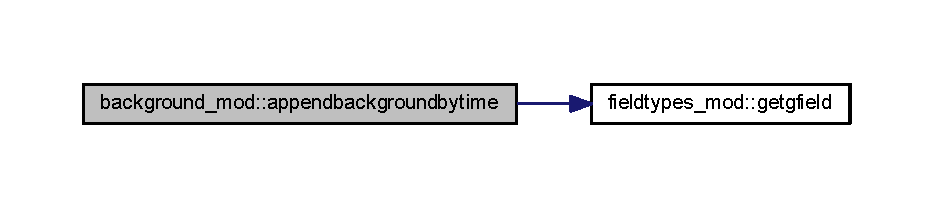
\includegraphics[width=350pt]{namespacebackground__mod_a02fa44cb4575159362bfa3b55520d387_cgraph}
\end{center}
\end{figure}
\mbox{\Hypertarget{namespacebackground__mod_af2f517e4aa946491744e012153045bd4}\label{namespacebackground__mod_af2f517e4aa946491744e012153045bd4}} 
\index{background\+\_\+mod@{background\+\_\+mod}!check@{check}}
\index{check@{check}!background\+\_\+mod@{background\+\_\+mod}}
\subsubsection{\texorpdfstring{check()}{check()}}
{\footnotesize\ttfamily logical function background\+\_\+mod\+::check (\begin{DoxyParamCaption}\item[{class(\mbox{\hyperlink{structbackground__mod_1_1background__class}{background\+\_\+class}}), intent(in)}]{self }\end{DoxyParamCaption})\hspace{0.3cm}{\ttfamily [private]}}



Method that checks the internal consistency of the fields within the background. 

\begin{DoxyAuthor}{Author}
Ricardo Birjukovs Canelas -\/ M\+A\+R\+E\+T\+EC 
\end{DoxyAuthor}


Definition at line 784 of file background.\+f90.


\begin{DoxyCode}
784     \textcolor{keywordtype}{class}(background\_class), \textcolor{keywordtype}{intent(in)} :: self
785     \textcolor{keywordtype}{integer}, \textcolor{keywordtype}{allocatable}, \textcolor{keywordtype}{dimension(:)} :: dimSize, fieldShape
786     \textcolor{keywordtype}{class}(*), \textcolor{keywordtype}{pointer} :: aField
787     \textcolor{keywordtype}{logical} :: equal
788     \textcolor{keywordtype}{integer} :: i
789     \textcolor{keywordtype}{type}(string) :: outext
790     check = .true.
791     equal = .true.
792     \textcolor{keywordflow}{if} (.not.self%initialized) check = .false.
793     \textcolor{keyword}{allocate}(dimsize(\textcolor{keyword}{size}(self%dim)))
794     \textcolor{keyword}{allocate}(fieldshape(\textcolor{keyword}{size}(self%dim)))
795     \textcolor{keywordflow}{do} i=1, \textcolor{keyword}{size}(self%dim)
796         dimsize(i) = \textcolor{keyword}{size}(self%dim(i)%field)
797 \textcolor{keywordflow}{    end do}
798     \textcolor{keyword}{call }self%fields%reset()               \textcolor{comment}{! reset list iterator}
799     \textcolor{keywordflow}{do} \textcolor{keywordflow}{while}(self%fields%moreValues())     \textcolor{comment}{! loop while there are values to process}
800         afield => self%fields%currentValue()
801         \textcolor{keywordflow}{select type}(afield)
802 \textcolor{keywordflow}{        class is} (field\_class)
803             equal = all(dimsize.eq.afield%getFieldShape())
804             \textcolor{keywordflow}{if} (.not.equal) check = .false.
805 \textcolor{keywordflow}{            class default}
806             outext = \textcolor{stringliteral}{'[background\_class::check] Unexepected type of content, not a scalar Field'}
807             \textcolor{keyword}{call }log%put(outext)
808             stop
809 \textcolor{keywordflow}{        end select}
810         \textcolor{keyword}{call }self%fields%next()            \textcolor{comment}{! increment the list iterator}
811 \textcolor{keywordflow}{    end do}
812     \textcolor{keyword}{call }self%fields%reset()               \textcolor{comment}{! reset list iterator}
813 
\end{DoxyCode}
\mbox{\Hypertarget{namespacebackground__mod_a1610fcc9ce260beb3c35418e92a63391}\label{namespacebackground__mod_a1610fcc9ce260beb3c35418e92a63391}} 
\index{background\+\_\+mod@{background\+\_\+mod}!cleanbackground@{cleanbackground}}
\index{cleanbackground@{cleanbackground}!background\+\_\+mod@{background\+\_\+mod}}
\subsubsection{\texorpdfstring{cleanbackground()}{cleanbackground()}}
{\footnotesize\ttfamily subroutine background\+\_\+mod\+::cleanbackground (\begin{DoxyParamCaption}\item[{class(\mbox{\hyperlink{structbackground__mod_1_1background__class}{background\+\_\+class}}), intent(inout)}]{self }\end{DoxyParamCaption})\hspace{0.3cm}{\ttfamily [private]}}



Method that cleans all data in the Background object. 

\begin{DoxyAuthor}{Author}
Ricardo Birjukovs Canelas -\/ M\+A\+R\+E\+T\+EC 
\end{DoxyAuthor}


Definition at line 569 of file background.\+f90.


\begin{DoxyCode}
569     \textcolor{keywordtype}{class}(background\_class), \textcolor{keywordtype}{intent(inout)} :: self
570     self%initialized = .false.
571     self%id = mv\_int
572     self%name = \textcolor{stringliteral}{''}
573     \textcolor{keywordflow}{if} (\textcolor{keyword}{allocated}(self%dim)) \textcolor{keyword}{deallocate}(self%dim)
574     \textcolor{keyword}{call }self%cleanFields()
575     \textcolor{keyword}{call }self%fields%finalize()
\end{DoxyCode}
\mbox{\Hypertarget{namespacebackground__mod_a843a471a68ce83809e3ed0a40886a4e7}\label{namespacebackground__mod_a843a471a68ce83809e3ed0a40886a4e7}} 
\index{background\+\_\+mod@{background\+\_\+mod}!cleanfields@{cleanfields}}
\index{cleanfields@{cleanfields}!background\+\_\+mod@{background\+\_\+mod}}
\subsubsection{\texorpdfstring{cleanfields()}{cleanfields()}}
{\footnotesize\ttfamily subroutine background\+\_\+mod\+::cleanfields (\begin{DoxyParamCaption}\item[{class(\mbox{\hyperlink{structbackground__mod_1_1background__class}{background\+\_\+class}}), intent(inout)}]{self }\end{DoxyParamCaption})\hspace{0.3cm}{\ttfamily [private]}}



Method that cleans all data in the Background object fields. 

\begin{DoxyAuthor}{Author}
Ricardo Birjukovs Canelas -\/ M\+A\+R\+E\+T\+EC 
\end{DoxyAuthor}


Definition at line 584 of file background.\+f90.


\begin{DoxyCode}
584     \textcolor{keywordtype}{class}(background\_class), \textcolor{keywordtype}{intent(inout)} :: self
585     \textcolor{keywordtype}{class}(*), \textcolor{keywordtype}{pointer} :: curr
586     \textcolor{keywordtype}{type}(string) :: outext
587     \textcolor{keyword}{call }self%fields%reset()               \textcolor{comment}{! reset list iterator}
588     \textcolor{keywordflow}{do} \textcolor{keywordflow}{while}(self%fields%moreValues())     \textcolor{comment}{! loop while there are values}
589         curr => self%fields%currentValue() \textcolor{comment}{! get current value}
590         \textcolor{keywordflow}{select type}(curr)
591 \textcolor{keywordflow}{        class is} (scalar1d\_field\_class)
592             \textcolor{keyword}{call }curr%finalize()
593 \textcolor{keywordflow}{        class is} (scalar2d\_field\_class)
594             \textcolor{keyword}{call }curr%finalize()
595 \textcolor{keywordflow}{        class is} (scalar3d\_field\_class)
596             \textcolor{keyword}{call }curr%finalize()
597 \textcolor{keywordflow}{        class is} (scalar4d\_field\_class)
598             \textcolor{keyword}{call }curr%finalize()
599 \textcolor{keywordflow}{            class default}
600             outext = \textcolor{stringliteral}{'[background\_class::cleanFields] Unexepected type of content, not a scalar Field'}
601             \textcolor{keyword}{call }log%put(outext)
602             stop
603 \textcolor{keywordflow}{        end select}
604         \textcolor{keyword}{call }self%fields%next()            \textcolor{comment}{! increment the list iterator}
605         \textcolor{keyword}{nullify}(curr)
606 \textcolor{keywordflow}{    end do}
607     \textcolor{keyword}{call }self%fields%reset()               \textcolor{comment}{! reset list iterator}
\end{DoxyCode}
\mbox{\Hypertarget{namespacebackground__mod_ad0096fb6a5a11854fd70a7ce58dc3000}\label{namespacebackground__mod_ad0096fb6a5a11854fd70a7ce58dc3000}} 
\index{background\+\_\+mod@{background\+\_\+mod}!constructor@{constructor}}
\index{constructor@{constructor}!background\+\_\+mod@{background\+\_\+mod}}
\subsubsection{\texorpdfstring{constructor()}{constructor()}}
{\footnotesize\ttfamily type(\mbox{\hyperlink{structbackground__mod_1_1background__class}{background\+\_\+class}}) function background\+\_\+mod\+::constructor (\begin{DoxyParamCaption}\item[{integer, intent(in)}]{id,  }\item[{type(string), intent(in)}]{name,  }\item[{type(\mbox{\hyperlink{structgeometry__mod_1_1box}{box}}), intent(in)}]{extents,  }\item[{type(scalar1d\+\_\+field\+\_\+class), dimension(\+:), intent(in)}]{dims }\end{DoxyParamCaption})\hspace{0.3cm}{\ttfamily [private]}}



Constructor for Background object. 

\begin{DoxyAuthor}{Author}
Ricardo Birjukovs Canelas -\/ M\+A\+R\+E\+T\+EC 
\end{DoxyAuthor}

\begin{DoxyParams}[1]{Parameters}
\mbox{\tt in}  & {\em id,name,extents,dims} & \\
\hline
\end{DoxyParams}


Definition at line 99 of file background.\+f90.


\begin{DoxyCode}
99     \textcolor{keywordtype}{type}(background\_class) :: constructor
100     \textcolor{keywordtype}{integer}, \textcolor{keywordtype}{intent(in)} :: id
101     \textcolor{keywordtype}{type}(string), \textcolor{keywordtype}{intent(in)} :: name
102     \textcolor{keywordtype}{type}(box), \textcolor{keywordtype}{intent(in)} :: extents
103     \textcolor{keywordtype}{type}(scalar1d\_field\_class), \textcolor{keywordtype}{dimension(:)}, \textcolor{keywordtype}{intent(in)} :: dims
104     constructor%initialized = .true.
105     \textcolor{keyword}{call }constructor%setID(id, name)
106     \textcolor{keyword}{call }constructor%setExtents(extents)
107     \textcolor{keyword}{call }constructor%setDims(dims)
\end{DoxyCode}
Here is the caller graph for this function\+:
\nopagebreak
\begin{figure}[H]
\begin{center}
\leavevmode
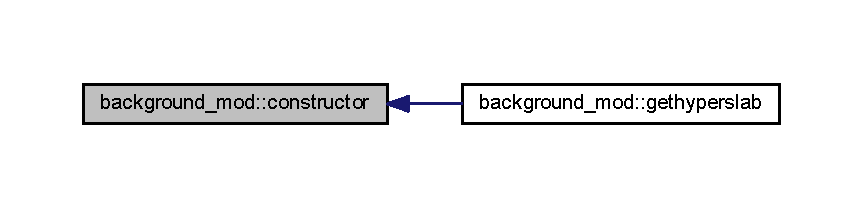
\includegraphics[width=350pt]{namespacebackground__mod_ad0096fb6a5a11854fd70a7ce58dc3000_icgraph}
\end{center}
\end{figure}
\mbox{\Hypertarget{namespacebackground__mod_a64c3966a113bc0f3b603c591bc345ca1}\label{namespacebackground__mod_a64c3966a113bc0f3b603c591bc345ca1}} 
\index{background\+\_\+mod@{background\+\_\+mod}!getdimextents@{getdimextents}}
\index{getdimextents@{getdimextents}!background\+\_\+mod@{background\+\_\+mod}}
\subsubsection{\texorpdfstring{getdimextents()}{getdimextents()}}
{\footnotesize\ttfamily real(prec) function, dimension(2) background\+\_\+mod\+::getdimextents (\begin{DoxyParamCaption}\item[{class(\mbox{\hyperlink{structbackground__mod_1_1background__class}{background\+\_\+class}}), intent(in)}]{self,  }\item[{type(string), intent(in)}]{name,  }\item[{logical, intent(in), optional}]{mandatory }\end{DoxyParamCaption})\hspace{0.3cm}{\ttfamily [private]}}



Method that returns two reals, min and max of a given dimension. 

\begin{DoxyAuthor}{Author}
Ricardo Birjukovs Canelas -\/ M\+A\+R\+E\+T\+EC 
\end{DoxyAuthor}

\begin{DoxyParams}[1]{Parameters}
\mbox{\tt in}  & {\em self,name,mandatory} & \\
\hline
\end{DoxyParams}


Definition at line 151 of file background.\+f90.


\begin{DoxyCode}
151     \textcolor{keywordtype}{class}(background\_class), \textcolor{keywordtype}{intent(in)} :: self
152     \textcolor{keywordtype}{type}(string), \textcolor{keywordtype}{intent(in)} :: name
153     \textcolor{keywordtype}{logical}, \textcolor{keywordtype}{optional}, \textcolor{keywordtype}{intent(in)} :: mandatory
154     \textcolor{keywordtype}{logical} :: mand
155     \textcolor{keywordtype}{integer} :: i
156     \textcolor{keywordtype}{real(prec)} :: dimExtent(2)
157     mand = .true.
158     \textcolor{keywordflow}{if} (\textcolor{keyword}{present}(mandatory)) mand = mandatory
159     i = self%getDimIndex(name, mand)
160     \textcolor{keywordflow}{if} ( i/= mv\_int) \textcolor{keywordflow}{then}
161         dimextent(1) = self%dim(i)%getFieldMinBound()
162         dimextent(2) = self%dim(i)%getFieldMaxBound()
163     \textcolor{keywordflow}{else}
164         dimextent(1) = mv
165         dimextent(2) = mv
166 \textcolor{keywordflow}{    end if}
\end{DoxyCode}
\mbox{\Hypertarget{namespacebackground__mod_a8a4c5fdcda63376bc3a984e9612dfb63}\label{namespacebackground__mod_a8a4c5fdcda63376bc3a984e9612dfb63}} 
\index{background\+\_\+mod@{background\+\_\+mod}!getdimindex@{getdimindex}}
\index{getdimindex@{getdimindex}!background\+\_\+mod@{background\+\_\+mod}}
\subsubsection{\texorpdfstring{getdimindex()}{getdimindex()}}
{\footnotesize\ttfamily integer function background\+\_\+mod\+::getdimindex (\begin{DoxyParamCaption}\item[{class(\mbox{\hyperlink{structbackground__mod_1_1background__class}{background\+\_\+class}}), intent(in)}]{self,  }\item[{type(string), intent(in)}]{name,  }\item[{logical, intent(in), optional}]{mandatory }\end{DoxyParamCaption})\hspace{0.3cm}{\ttfamily [private]}}



Method that returns the index of a given dimension by it\textquotesingle{}s name. 

\begin{DoxyAuthor}{Author}
Ricardo Birjukovs Canelas -\/ M\+A\+R\+E\+T\+EC 
\end{DoxyAuthor}

\begin{DoxyParams}[1]{Parameters}
\mbox{\tt in}  & {\em self,name,mandatory} & \\
\hline
\end{DoxyParams}


Definition at line 117 of file background.\+f90.


\begin{DoxyCode}
117     \textcolor{keywordtype}{class}(background\_class), \textcolor{keywordtype}{intent(in)} :: self
118     \textcolor{keywordtype}{type}(string), \textcolor{keywordtype}{intent(in)} :: name
119     \textcolor{keywordtype}{logical}, \textcolor{keywordtype}{optional}, \textcolor{keywordtype}{intent(in)} :: mandatory
120     \textcolor{keywordtype}{integer} :: i
121     \textcolor{keywordtype}{type}(string) :: outext
122     \textcolor{keywordtype}{logical} found
123     found = .false.
124     \textcolor{keywordflow}{do} i=1, \textcolor{keyword}{size}(self%dim)
125         \textcolor{keywordflow}{if} (self%dim(i)%name == name) \textcolor{keywordflow}{then}
126             found = .true.
127             getdimindex = i
128             \textcolor{keywordflow}{return}
129 \textcolor{keywordflow}{        end if}
130 \textcolor{keywordflow}{    end do}
131     \textcolor{keywordflow}{if} (\textcolor{keyword}{present}(mandatory)) \textcolor{keywordflow}{then}
132         \textcolor{keywordflow}{if} (mandatory) \textcolor{keywordflow}{then}
133             \textcolor{keywordflow}{if} (.not. found) \textcolor{keywordflow}{then}
134                 outext = \textcolor{stringliteral}{'[background\_class::getDimIndex]: Field dimensions dont contain a field called '}//
       name //\textcolor{stringliteral}{', stoping'}
135                 \textcolor{keyword}{call }log%put(outext)
136                 stop
137 \textcolor{keywordflow}{            end if}
138         \textcolor{keywordflow}{else}
139             getdimindex = mv\_int
140 \textcolor{keywordflow}{        end if}
141 \textcolor{keywordflow}{    end if}
\end{DoxyCode}
\mbox{\Hypertarget{namespacebackground__mod_ae26fda3baab915148ec5749d1eda2ea6}\label{namespacebackground__mod_ae26fda3baab915148ec5749d1eda2ea6}} 
\index{background\+\_\+mod@{background\+\_\+mod}!gethyperslab@{gethyperslab}}
\index{gethyperslab@{gethyperslab}!background\+\_\+mod@{background\+\_\+mod}}
\subsubsection{\texorpdfstring{gethyperslab()}{gethyperslab()}}
{\footnotesize\ttfamily type(\mbox{\hyperlink{structbackground__mod_1_1background__class}{background\+\_\+class}}) function background\+\_\+mod\+::gethyperslab (\begin{DoxyParamCaption}\item[{class(\mbox{\hyperlink{structbackground__mod_1_1background__class}{background\+\_\+class}}), intent(in)}]{self,  }\item[{type(\mbox{\hyperlink{structgeometry__mod_1_1box}{box}}), intent(in)}]{domain,  }\item[{real(prec), dimension(2), intent(in), optional}]{time }\end{DoxyParamCaption})\hspace{0.3cm}{\ttfamily [private]}}



returns a background as a subset of another 

\begin{DoxyAuthor}{Author}
Ricardo Birjukovs Canelas -\/ M\+A\+R\+E\+T\+EC 
\end{DoxyAuthor}

\begin{DoxyParams}[1]{Parameters}
\mbox{\tt in}  & {\em self,domain,time} & \\
\hline
\end{DoxyParams}


Definition at line 276 of file background.\+f90.


\begin{DoxyCode}
276     \textcolor{keywordtype}{class}(background\_class), \textcolor{keywordtype}{intent(in)} :: self
277     \textcolor{keywordtype}{type}(box), \textcolor{keywordtype}{intent(in)} :: domain
278     \textcolor{keywordtype}{real(prec)}, \textcolor{keywordtype}{intent(in)}, \textcolor{keywordtype}{optional} :: time(2)
279     \textcolor{keywordtype}{real(prec)} :: ltime(2)
280     \textcolor{keywordtype}{type}(scalar1d\_field\_class), \textcolor{keywordtype}{allocatable}, \textcolor{keywordtype}{dimension(:)} :: backgrounDims
281     \textcolor{keywordtype}{type}(generic\_field\_class), \textcolor{keywordtype}{allocatable}, \textcolor{keywordtype}{dimension(:)} :: gfield
282     \textcolor{keywordtype}{class}(*), \textcolor{keywordtype}{pointer} :: curr
283     \textcolor{keywordtype}{type}(box) :: extents
284     \textcolor{keywordtype}{type}(vector) :: pt
285     \textcolor{keywordtype}{real(prec)}, \textcolor{keywordtype}{dimension(3,2)} :: dimExtents
286     \textcolor{keywordtype}{integer}, \textcolor{keywordtype}{allocatable}, \textcolor{keywordtype}{dimension(:)} :: llbound
287     \textcolor{keywordtype}{integer}, \textcolor{keywordtype}{allocatable}, \textcolor{keywordtype}{dimension(:)} :: uubound
288     \textcolor{keywordtype}{integer} :: temp\_int
289     \textcolor{keywordtype}{type}(string) :: outext
290     \textcolor{keywordtype}{integer} :: i
291 
292     ltime = self%getDimExtents(globals%Var%time)
293     \textcolor{keywordflow}{if} (\textcolor{keyword}{present}(time)) ltime = time
294     \textcolor{comment}{!finding index bounds of the slicing geometry}
295     \textcolor{keyword}{allocate}(llbound(\textcolor{keyword}{size}(self%dim)))
296     \textcolor{keyword}{allocate}(uubound(\textcolor{keyword}{size}(self%dim)))
297     llbound = self%getPointDimIndexes(domain%pt, ltime(1))
298     uubound = self%getPointDimIndexes(domain%pt+domain%size, ltime(2))
299     \textcolor{comment}{!slicing dimensions}
300     \textcolor{keyword}{allocate}(backgroundims(\textcolor{keyword}{size}(self%dim)))
301     \textcolor{keywordflow}{do} i=1, \textcolor{keyword}{size}(self%dim)
302         \textcolor{keywordflow}{if} (llbound(i) > uubound(i)) \textcolor{keywordflow}{then} \textcolor{comment}{!because We're not inverting the dimension and fields - Needs to
       be corrected}
303             temp\_int = llbound(i)
304             llbound(i) = uubound(i)
305             uubound(i) = temp\_int
306 \textcolor{keywordflow}{        end if}
307         llbound(i) = max(1, llbound(i)-1) \textcolor{comment}{!adding safety net to index bounds}
308         uubound(i) = min(uubound(i)+1, \textcolor{keyword}{size}(self%dim(i)%field))
309         \textcolor{keyword}{call }backgroundims(i)%initialize(self%dim(i)%name, self%dim(i)%units, 1, self%getSlabDim(i, llbound
      (i), uubound(i)))
310 \textcolor{keywordflow}{    end do}
311     \textcolor{comment}{!slicing variables}
312     \textcolor{keyword}{allocate}(gfield(self%fields%getSize()))
313     i=1
314     \textcolor{keyword}{call }self%fields%reset()               \textcolor{comment}{! reset list iterator}
315     \textcolor{keywordflow}{do} \textcolor{keywordflow}{while}(self%fields%moreValues())     \textcolor{comment}{! loop while there are values}
316         curr => self%fields%currentValue() \textcolor{comment}{! get current value}
317         \textcolor{keywordflow}{select type}(curr)
318 \textcolor{keywordflow}{        class is} (field\_class)
319             gfield(i) = curr%getFieldSlice(llbound, uubound)
320 \textcolor{keywordflow}{            class default}
321             outext = \textcolor{stringliteral}{'[background\_class::getHyperSlab] Unexepected type of content, not a scalar Field'}
322             \textcolor{keyword}{call }log%put(outext)
323             stop
324 \textcolor{keywordflow}{        end select}
325         \textcolor{keyword}{call }self%fields%next()            \textcolor{comment}{! increment the list iterator}
326         i = i+1
327         \textcolor{keyword}{nullify}(curr)
328 \textcolor{keywordflow}{    end do}
329     \textcolor{keyword}{call }self%fields%reset()               \textcolor{comment}{! reset list iterator}
330     \textcolor{comment}{!creating bounding box}
331     dimextents = 0.0
332     \textcolor{keywordflow}{do} i = 1, \textcolor{keyword}{size}(backgroundims)
333         \textcolor{keywordflow}{if} (backgroundims(i)%name == globals%Var%lon) \textcolor{keywordflow}{then}
334             dimextents(1,1) = backgroundims(i)%getFieldMinBound()
335             dimextents(1,2) = backgroundims(i)%getFieldMaxBound()
336         \textcolor{keywordflow}{else} \textcolor{keywordflow}{if} (backgroundims(i)%name == globals%Var%lat) \textcolor{keywordflow}{then}
337             dimextents(2,1) = backgroundims(i)%getFieldMinBound()
338             dimextents(2,2) = backgroundims(i)%getFieldMaxBound()
339         \textcolor{keywordflow}{else} \textcolor{keywordflow}{if} (backgroundims(i)%name == globals%Var%level) \textcolor{keywordflow}{then}
340             dimextents(3,1) = backgroundims(i)%getFieldMinBound()
341             dimextents(3,2) = backgroundims(i)%getFieldMaxBound()
342 \textcolor{keywordflow}{        end if}
343 \textcolor{keywordflow}{    end do}
344     extents%pt = dimextents(1,1)*ex + dimextents(2,1)*ey + dimextents(3,1)*ez
345     pt = dimextents(1,2)*ex + dimextents(2,2)*ey + dimextents(3,2)*ez
346     extents%size = pt - extents%pt
347     \textcolor{comment}{!creating the sliced background}
348     gethyperslab = constructor(1, self%name, extents, backgroundims)
349     \textcolor{keywordflow}{do} i=1, \textcolor{keyword}{size}(gfield)
350         \textcolor{keyword}{call }gethyperslab%add(gfield(i))
351         \textcolor{keyword}{call }gfield(i)%finalize()
352 \textcolor{keywordflow}{    end do}
353 
354     \textcolor{keywordflow}{if}(.not.self%check()) \textcolor{keywordflow}{then}
355         outext = \textcolor{stringliteral}{'[Background::getHyperSlab]: non-conformant Background, stoping '}
356         \textcolor{keyword}{call }log%put(outext)
357         stop
358 \textcolor{keywordflow}{    end if}
359 
\end{DoxyCode}
Here is the call graph for this function\+:
\nopagebreak
\begin{figure}[H]
\begin{center}
\leavevmode
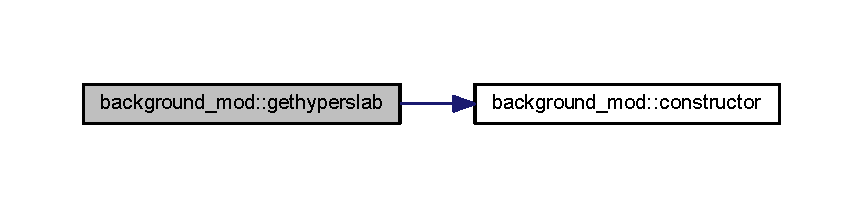
\includegraphics[width=350pt]{namespacebackground__mod_ae26fda3baab915148ec5749d1eda2ea6_cgraph}
\end{center}
\end{figure}
\mbox{\Hypertarget{namespacebackground__mod_ac799224ce7ad219bf1fb4f1f42508f45}\label{namespacebackground__mod_ac799224ce7ad219bf1fb4f1f42508f45}} 
\index{background\+\_\+mod@{background\+\_\+mod}!getpointdimindexes@{getpointdimindexes}}
\index{getpointdimindexes@{getpointdimindexes}!background\+\_\+mod@{background\+\_\+mod}}
\subsubsection{\texorpdfstring{getpointdimindexes()}{getpointdimindexes()}}
{\footnotesize\ttfamily integer function, dimension(\+:), allocatable background\+\_\+mod\+::getpointdimindexes (\begin{DoxyParamCaption}\item[{class(\mbox{\hyperlink{structbackground__mod_1_1background__class}{background\+\_\+class}}), intent(in)}]{self,  }\item[{type(vector), intent(in)}]{pt,  }\item[{real(prec), intent(in)}]{time }\end{DoxyParamCaption})\hspace{0.3cm}{\ttfamily [private]}}



returns the indexes of the dims for a given point 

\begin{DoxyAuthor}{Author}
Ricardo Birjukovs Canelas -\/ M\+A\+R\+E\+T\+EC 
\end{DoxyAuthor}

\begin{DoxyParams}[1]{Parameters}
\mbox{\tt in}  & {\em self,pt,time} & \\
\hline
\end{DoxyParams}


Definition at line 369 of file background.\+f90.


\begin{DoxyCode}
369     \textcolor{keywordtype}{class}(background\_class), \textcolor{keywordtype}{intent(in)} :: self
370     \textcolor{keywordtype}{type}(vector), \textcolor{keywordtype}{intent(in)} :: pt
371     \textcolor{keywordtype}{real(prec)}, \textcolor{keywordtype}{intent(in)} :: time
372     \textcolor{keywordtype}{integer}, \textcolor{keywordtype}{allocatable}, \textcolor{keywordtype}{dimension(:)} :: getPointDimIndexes
373     \textcolor{keywordtype}{integer} :: i
374     \textcolor{keyword}{allocate}(getpointdimindexes(\textcolor{keyword}{size}(self%dim)))
375     \textcolor{keywordflow}{do} i= 1, \textcolor{keyword}{size}(self%dim)
376         \textcolor{keywordflow}{if} (self%dim(i)%name == globals%Var%lon) getpointdimindexes(i) = self%dim(i)%getFieldNearestIndex(
      pt%x)
377         \textcolor{keywordflow}{if} (self%dim(i)%name == globals%Var%lat) getpointdimindexes(i) = self%dim(i)%getFieldNearestIndex(
      pt%y)
378         \textcolor{keywordflow}{if} (self%dim(i)%name == globals%Var%level) getpointdimindexes(i) = self%dim(i)%getFieldNearestIndex
      (pt%z)
379         \textcolor{keywordflow}{if} (self%dim(i)%name == globals%Var%time)  getpointdimindexes(i) = self%dim(i)%getFieldNearestIndex
      (time)
380 \textcolor{keywordflow}{    end do}
\end{DoxyCode}
\mbox{\Hypertarget{namespacebackground__mod_a09d61976c4545e8753eb4594044b109d}\label{namespacebackground__mod_a09d61976c4545e8753eb4594044b109d}} 
\index{background\+\_\+mod@{background\+\_\+mod}!getslabdim@{getslabdim}}
\index{getslabdim@{getslabdim}!background\+\_\+mod@{background\+\_\+mod}}
\subsubsection{\texorpdfstring{getslabdim()}{getslabdim()}}
{\footnotesize\ttfamily real(prec) function, dimension(\+:), allocatable background\+\_\+mod\+::getslabdim (\begin{DoxyParamCaption}\item[{class(\mbox{\hyperlink{structbackground__mod_1_1background__class}{background\+\_\+class}}), intent(in)}]{self,  }\item[{integer, intent(in)}]{num\+Dim,  }\item[{integer, intent(in)}]{llbound,  }\item[{integer, intent(in)}]{uubound }\end{DoxyParamCaption})\hspace{0.3cm}{\ttfamily [private]}}



returns an array witn a sliced dimension 

\begin{DoxyAuthor}{Author}
Ricardo Birjukovs Canelas -\/ M\+A\+R\+E\+T\+EC 
\end{DoxyAuthor}

\begin{DoxyParams}[1]{Parameters}
\mbox{\tt in}  & {\em self,domain,time} & \\
\hline
\end{DoxyParams}


Definition at line 390 of file background.\+f90.


\begin{DoxyCode}
390     \textcolor{keywordtype}{class}(background\_class), \textcolor{keywordtype}{intent(in)} :: self
391     \textcolor{keywordtype}{integer}, \textcolor{keywordtype}{intent(in)} :: numDim, llbound, uubound
392     \textcolor{keywordtype}{real(prec)}, \textcolor{keywordtype}{allocatable}, \textcolor{keywordtype}{dimension(:)} :: getSlabDim
393     \textcolor{keyword}{allocate}(getslabdim, source = self%dim(numdim)%field(llbound:uubound))
\end{DoxyCode}
\mbox{\Hypertarget{namespacebackground__mod_ad6c54d2cf1d1981fb928cd14d387aa8b}\label{namespacebackground__mod_ad6c54d2cf1d1981fb928cd14d387aa8b}} 
\index{background\+\_\+mod@{background\+\_\+mod}!makelandmask@{makelandmask}}
\index{makelandmask@{makelandmask}!background\+\_\+mod@{background\+\_\+mod}}
\subsubsection{\texorpdfstring{makelandmask()}{makelandmask()}}
{\footnotesize\ttfamily subroutine background\+\_\+mod\+::makelandmask (\begin{DoxyParamCaption}\item[{class(\mbox{\hyperlink{structbackground__mod_1_1background__class}{background\+\_\+class}}), intent(inout)}]{self }\end{DoxyParamCaption})\hspace{0.3cm}{\ttfamily [private]}}



Method to use a stored binary field to make a land mask used for land interaction\+: bed settling, beaching, ... 

\begin{DoxyAuthor}{Author}
Ricardo Birjukovs Canelas -\/ M\+A\+R\+E\+T\+EC 
\end{DoxyAuthor}


Definition at line 488 of file background.\+f90.


\begin{DoxyCode}
488     \textcolor{keywordtype}{class}(background\_class), \textcolor{keywordtype}{intent(inout)} :: self
489     \textcolor{keywordtype}{class}(*), \textcolor{keywordtype}{pointer} :: curr
490     \textcolor{keywordtype}{logical}, \textcolor{keywordtype}{allocatable}, \textcolor{keywordtype}{dimension(:,:,:)} :: shiftleftlon3d, shiftuplat3d, shiftrigthlon3d, shiftdownlat3d
      , beach3d
491     \textcolor{keywordtype}{logical}, \textcolor{keywordtype}{allocatable}, \textcolor{keywordtype}{dimension(:,:,:,:)} :: shiftleftlon4d, shiftuplat4d, shiftrigthlon4d, 
      shiftdownlat4d, shiftUpLevel, shiftDownLevel, beach4d, bed4d
492     \textcolor{keywordtype}{type}(string) :: outext
493     \textcolor{keywordtype}{integer} :: dimIndx
494     \textcolor{keyword}{call }self%fields%reset()               \textcolor{comment}{! reset list iterator}
495     \textcolor{keywordflow}{do} \textcolor{keywordflow}{while}(self%fields%moreValues())     \textcolor{comment}{! loop while there are values}
496         curr => self%fields%currentValue() \textcolor{comment}{! get current value        }
497             \textcolor{keywordflow}{select type}(curr)            
498 \textcolor{keywordflow}{            class is} (scalar3d\_field\_class)
499                 \textcolor{keywordflow}{if} (curr%name == globals%Var%landIntMask) \textcolor{keywordflow}{then}
500                     \textcolor{keyword}{allocate}(shiftleftlon3d(\textcolor{keyword}{size}(curr%field,1), \textcolor{keyword}{size}(curr%field,2), \textcolor{keyword}{size}(curr%field,3)))
501                     \textcolor{keyword}{allocate}(shiftuplat3d(\textcolor{keyword}{size}(curr%field,1), \textcolor{keyword}{size}(curr%field,2), \textcolor{keyword}{size}(curr%field,3)))
502                     \textcolor{keyword}{allocate}(shiftrigthlon3d(\textcolor{keyword}{size}(curr%field,1), \textcolor{keyword}{size}(curr%field,2), \textcolor{keyword}{size}(curr%field,3)))
503                     \textcolor{keyword}{allocate}(shiftdownlat3d(\textcolor{keyword}{size}(curr%field,1), \textcolor{keyword}{size}(curr%field,2), \textcolor{keyword}{size}(curr%field,3)))
504                     \textcolor{keyword}{allocate}(beach3d(\textcolor{keyword}{size}(curr%field,1), \textcolor{keyword}{size}(curr%field,2), \textcolor{keyword}{size}(curr%field,3)))
505                     shiftleftlon3d = .false.
506                     shiftleftlon3d(:\textcolor{keyword}{size}(curr%field,1)-1,:,:) = abs(curr%field(:\textcolor{keyword}{size}(curr%field,1)-1,:,:) -
       curr%field(2:,:,:)) == globals%Mask%waterVal - globals%Mask%landVal
507                     shiftrigthlon3d = .false.
508                     shiftrigthlon3d(2:,:,:) = abs(curr%field(2:,:,:) - curr%field(:\textcolor{keyword}{size}(curr%field,1)-1,:,:
      )) == globals%Mask%waterVal - globals%Mask%landVal
509                     shiftuplat3d = .false.
510                     shiftuplat3d(:,:\textcolor{keyword}{size}(curr%field,2)-1,:) = abs(curr%field(:,:\textcolor{keyword}{size}(curr%field,2)-1,:) - 
      curr%field(:,2:,:)) == globals%Mask%waterVal - globals%Mask%landVal
511                     shiftdownlat3d = .false.
512                     shiftdownlat3d(:, 2:,:) = abs(curr%field(:,2:,:) - curr%field(:,:\textcolor{keyword}{size}(curr%field,2)-1,:
      )) == globals%Mask%waterVal - globals%Mask%landVal
513                     beach3d = .false.
514                     beach3d = shiftleftlon3d .or. shiftrigthlon3d .or. shiftuplat3d .or. shiftdownlat3d \textcolor{comment}{
      !colapsing all the shifts}
515                     beach3d = beach3d .and. (curr%field == globals%Mask%landVal) \textcolor{comment}{!just points that were
       already wet}
516                     \textcolor{keywordflow}{where}(beach3d) curr%field = globals%Mask%beachVal
517 \textcolor{keywordflow}{                end if}
518 \textcolor{keywordflow}{            class is} (scalar4d\_field\_class)
519                 \textcolor{keywordflow}{if} (curr%name == globals%Var%landIntMask) \textcolor{keywordflow}{then}
520                     \textcolor{keyword}{allocate}(shiftleftlon4d(\textcolor{keyword}{size}(curr%field,1), \textcolor{keyword}{size}(curr%field,2), \textcolor{keyword}{size}(curr%field,3), \textcolor{keyword}{
      size}(curr%field,4)))
521                     \textcolor{keyword}{allocate}(shiftuplat4d(\textcolor{keyword}{size}(curr%field,1), \textcolor{keyword}{size}(curr%field,2), \textcolor{keyword}{size}(curr%field,3), \textcolor{keyword}{size}(
      curr%field,4)))
522                     \textcolor{keyword}{allocate}(shiftrigthlon4d(\textcolor{keyword}{size}(curr%field,1), \textcolor{keyword}{size}(curr%field,2), \textcolor{keyword}{size}(curr%field,3), \textcolor{keyword}{
      size}(curr%field,4)))
523                     \textcolor{keyword}{allocate}(shiftdownlat4d(\textcolor{keyword}{size}(curr%field,1), \textcolor{keyword}{size}(curr%field,2), \textcolor{keyword}{size}(curr%field,3), \textcolor{keyword}{
      size}(curr%field,4)))
524                     \textcolor{keyword}{allocate}(shiftuplevel(\textcolor{keyword}{size}(curr%field,1), \textcolor{keyword}{size}(curr%field,2), \textcolor{keyword}{size}(curr%field,3), \textcolor{keyword}{size}(
      curr%field,4)))
525                     \textcolor{keyword}{allocate}(shiftdownlevel(\textcolor{keyword}{size}(curr%field,1), \textcolor{keyword}{size}(curr%field,2), \textcolor{keyword}{size}(curr%field,3), \textcolor{keyword}{
      size}(curr%field,4)))
526                     \textcolor{keyword}{allocate}(beach4d(\textcolor{keyword}{size}(curr%field,1), \textcolor{keyword}{size}(curr%field,2), \textcolor{keyword}{size}(curr%field,3), \textcolor{keyword}{size}(curr
      %field,4)))
527                     \textcolor{keyword}{allocate}(bed4d(\textcolor{keyword}{size}(curr%field,1), \textcolor{keyword}{size}(curr%field,2), \textcolor{keyword}{size}(curr%field,3), \textcolor{keyword}{size}(curr
      %field,4)))
528                     shiftleftlon4d = .false.
529                     shiftleftlon4d(:\textcolor{keyword}{size}(curr%field,1)-1,:,:,:) = abs(curr%field(:\textcolor{keyword}{size}(curr%field,1)-1,:,:,
      :) - curr%field(2:,:,:,:)) /= 0.0
530                     shiftrigthlon4d = .false.
531                     shiftrigthlon4d(2:,:,:,:) = abs(curr%field(2:,:,:,:) - curr%field(:\textcolor{keyword}{size}(curr%field,1)-1
      ,:,:,:)) /= 0.0
532                     shiftdownlat4d = .false.
533                     shiftdownlat4d(:,:\textcolor{keyword}{size}(curr%field,2)-1,:,:) = abs(curr%field(:,:\textcolor{keyword}{size}(curr%field,2)-1,:,
      :) - curr%field(:,2:,:,:)) /= 0.0
534                     shiftuplat4d = .false.
535                     shiftuplat4d(:,2:,:,:) = abs(curr%field(:,2:,:,:) - curr%field(:,:\textcolor{keyword}{size}(curr%field,2)-1,
      :,:)) /= 0.0
536                     shiftuplevel = .false.
537                     shiftuplevel(:,:,2:,:) = abs(curr%field(:,:,2:,:) - curr%field(:,:,:\textcolor{keyword}{size}(curr%field,3)-
      1,:)) /= 0.0
538                     shiftdownlevel = .false.
539                     shiftdownlevel(:,:,:\textcolor{keyword}{size}(curr%field,3)-1,:) = abs(curr%field(:,:,:\textcolor{keyword}{size}(curr%field,3)-1,
      :) - curr%field(:,:,2:,:)) /= 0.0
540                     beach4d = .false.
541                     beach4d = shiftleftlon4d .or. shiftrigthlon4d .or. shiftuplat4d .or. shiftdownlat4d 
      .or. shiftdownlevel .or. shiftuplevel \textcolor{comment}{!colapsing all the shifts                    }
542                     \textcolor{comment}{!beach4d = beach4d .and. (curr%field == Globals%Mask%landVal) !just points that were
       already wet}
543                     bed4d = beach4d
544                     dimindx = self%getDimIndex(globals%Var%level)
545                     dimindx = minloc(abs(self%dim(dimindx)%field - globals%Constants%BeachingLevel),1)
546                     beach4d(:,:,:dimindx,:) = .false. \textcolor{comment}{!this must be above a certain level only}
547                     bed4d(:,:,dimindx:,:) = .false.   \textcolor{comment}{!bellow a certain level}
548                     \textcolor{keywordflow}{where}(beach4d) curr%field = globals%Mask%beachVal
549                     \textcolor{keywordflow}{where}(bed4d) curr%field = globals%Mask%bedVal
550 \textcolor{keywordflow}{                end if}                
551 \textcolor{keywordflow}{                class default}
552                 outext = \textcolor{stringliteral}{'[background\_class::makeLandMask] Unexepected type of content, not a 3D or 4D
       scalar Field'}
553                 \textcolor{keyword}{call }log%put(outext)
554                 stop
555 \textcolor{keywordflow}{            end select}       
556         \textcolor{keyword}{call }self%fields%next()            \textcolor{comment}{! increment the list iterator}
557         \textcolor{keyword}{nullify}(curr)
558 \textcolor{keywordflow}{    end do}
559     \textcolor{keyword}{call }self%fields%reset()               \textcolor{comment}{! reset list iterator}
560     
\end{DoxyCode}
\mbox{\Hypertarget{namespacebackground__mod_acdcc52b4fb298bc145a121f9e8a4b929}\label{namespacebackground__mod_acdcc52b4fb298bc145a121f9e8a4b929}} 
\index{background\+\_\+mod@{background\+\_\+mod}!print\+\_\+fieldlist@{print\+\_\+fieldlist}}
\index{print\+\_\+fieldlist@{print\+\_\+fieldlist}!background\+\_\+mod@{background\+\_\+mod}}
\subsubsection{\texorpdfstring{print\+\_\+fieldlist()}{print\_fieldlist()}}
{\footnotesize\ttfamily subroutine background\+\_\+mod\+::print\+\_\+fieldlist (\begin{DoxyParamCaption}\item[{class(\mbox{\hyperlink{structbackground__mod_1_1fieldslist__class}{fieldslist\+\_\+class}}), intent(in)}]{this }\end{DoxyParamCaption})\hspace{0.3cm}{\ttfamily [private]}}



Method that prints all the links of the list. 

\begin{DoxyAuthor}{Author}
Ricardo Birjukovs Canelas -\/ M\+A\+R\+E\+T\+EC 
\end{DoxyAuthor}


Definition at line 748 of file background.\+f90.


\begin{DoxyCode}
748     \textcolor{keywordtype}{class}(fieldsList\_class), \textcolor{keywordtype}{intent(in)} :: this
749     \textcolor{keyword}{call }this%reset()               \textcolor{comment}{! reset list iterator}
750     \textcolor{keywordflow}{do} \textcolor{keywordflow}{while}(this%moreValues())     \textcolor{comment}{! loop while there are values to print}
751         \textcolor{keyword}{call }this%printCurrent()
752         \textcolor{keyword}{call }this%next()            \textcolor{comment}{! increment the list iterator}
753 \textcolor{keywordflow}{    end do}
754     \textcolor{keyword}{call }this%reset()               \textcolor{comment}{! reset list iterator}
\end{DoxyCode}
\mbox{\Hypertarget{namespacebackground__mod_a2bd18f3830c0667741efd086d36753db}\label{namespacebackground__mod_a2bd18f3830c0667741efd086d36753db}} 
\index{background\+\_\+mod@{background\+\_\+mod}!print\+\_\+fieldlistcurrent@{print\+\_\+fieldlistcurrent}}
\index{print\+\_\+fieldlistcurrent@{print\+\_\+fieldlistcurrent}!background\+\_\+mod@{background\+\_\+mod}}
\subsubsection{\texorpdfstring{print\+\_\+fieldlistcurrent()}{print\_fieldlistcurrent()}}
{\footnotesize\ttfamily subroutine background\+\_\+mod\+::print\+\_\+fieldlistcurrent (\begin{DoxyParamCaption}\item[{class(\mbox{\hyperlink{structbackground__mod_1_1fieldslist__class}{fieldslist\+\_\+class}}), intent(in)}]{this }\end{DoxyParamCaption})\hspace{0.3cm}{\ttfamily [private]}}



Method that prints the current link of the list. 

\begin{DoxyAuthor}{Author}
Ricardo Birjukovs Canelas -\/ M\+A\+R\+E\+T\+EC 
\end{DoxyAuthor}


Definition at line 763 of file background.\+f90.


\begin{DoxyCode}
763     \textcolor{keywordtype}{class}(fieldsList\_class), \textcolor{keywordtype}{intent(in)} :: this
764     \textcolor{keywordtype}{class}(*), \textcolor{keywordtype}{pointer} :: curr
765     \textcolor{keywordtype}{type}(string) :: outext
766     curr => this%currentValue() \textcolor{comment}{! get current value}
767     \textcolor{keywordflow}{select type}(curr)
768 \textcolor{keywordflow}{    class is} (field\_class)
769         \textcolor{keyword}{call }curr%print()
770 \textcolor{keywordflow}{        class default}
771         outext = \textcolor{stringliteral}{'[fieldsList\_class::print] Unexepected type of content, not a Field'}
772         \textcolor{keyword}{call }log%put(outext)
773         stop
774 \textcolor{keywordflow}{    end select}
\end{DoxyCode}
\mbox{\Hypertarget{namespacebackground__mod_a8a8f225cffcddb742f22a402155b703f}\label{namespacebackground__mod_a8a8f225cffcddb742f22a402155b703f}} 
\index{background\+\_\+mod@{background\+\_\+mod}!printbackground@{printbackground}}
\index{printbackground@{printbackground}!background\+\_\+mod@{background\+\_\+mod}}
\subsubsection{\texorpdfstring{printbackground()}{printbackground()}}
{\footnotesize\ttfamily subroutine background\+\_\+mod\+::printbackground (\begin{DoxyParamCaption}\item[{class(\mbox{\hyperlink{structbackground__mod_1_1background__class}{background\+\_\+class}}), intent(inout)}]{self }\end{DoxyParamCaption})\hspace{0.3cm}{\ttfamily [private]}}



Method that prints the Background object. 

\begin{DoxyAuthor}{Author}
Ricardo Birjukovs Canelas -\/ M\+A\+R\+E\+T\+EC 
\end{DoxyAuthor}


Definition at line 725 of file background.\+f90.


\begin{DoxyCode}
725     \textcolor{keywordtype}{class}(background\_class), \textcolor{keywordtype}{intent(inout)} :: self
726     \textcolor{keywordtype}{type}(string) :: outext, t
727     \textcolor{keywordtype}{integer} :: i
728     t = self%id
729     outext = \textcolor{stringliteral}{'Background['}//t//\textcolor{stringliteral}{', '}//self%name//\textcolor{stringliteral}{'] is a'}
730     \textcolor{keyword}{call }log%put(outext,.false.)
731     \textcolor{keyword}{call }geometry%print(self%extents)
732     outext = \textcolor{stringliteral}{'The dimensions fields are:'}
733     \textcolor{keyword}{call }log%put(outext,.false.)
734     \textcolor{keywordflow}{do} i=1, \textcolor{keyword}{size}(self%dim)
735         \textcolor{keyword}{call }self%dim(i)%print()
736 \textcolor{keywordflow}{    end do}
737     outext = \textcolor{stringliteral}{'The data fields are:'}
738     \textcolor{keyword}{call }log%put(outext,.false.)
739     \textcolor{keyword}{call }self%fields%print()
\end{DoxyCode}
\mbox{\Hypertarget{namespacebackground__mod_a06d96d4627391d74feb105a842a87dc0}\label{namespacebackground__mod_a06d96d4627391d74feb105a842a87dc0}} 
\index{background\+\_\+mod@{background\+\_\+mod}!setdims@{setdims}}
\index{setdims@{setdims}!background\+\_\+mod@{background\+\_\+mod}}
\subsubsection{\texorpdfstring{setdims()}{setdims()}}
{\footnotesize\ttfamily subroutine background\+\_\+mod\+::setdims (\begin{DoxyParamCaption}\item[{class(\mbox{\hyperlink{structbackground__mod_1_1background__class}{background\+\_\+class}}), intent(inout)}]{self,  }\item[{type(scalar1d\+\_\+field\+\_\+class), dimension(\+:), intent(in)}]{dims }\end{DoxyParamCaption})\hspace{0.3cm}{\ttfamily [private]}}



Method that allocates and sets the dimensions of the Background object. 

\begin{DoxyAuthor}{Author}
Ricardo Birjukovs Canelas -\/ M\+A\+R\+E\+T\+EC 
\end{DoxyAuthor}

\begin{DoxyParams}[1]{Parameters}
\mbox{\tt in}  & {\em self,dims} & \\
\hline
\end{DoxyParams}


Definition at line 617 of file background.\+f90.


\begin{DoxyCode}
617     \textcolor{keywordtype}{class}(background\_class), \textcolor{keywordtype}{intent(inout)} :: self
618     \textcolor{keywordtype}{type}(scalar1d\_field\_class), \textcolor{keywordtype}{dimension(:)}, \textcolor{keywordtype}{intent(in)} :: dims
619     \textcolor{keywordtype}{real(prec)}, \textcolor{keywordtype}{allocatable}, \textcolor{keywordtype}{dimension(:)} :: rest
620     \textcolor{keywordtype}{integer} :: i
621     \textcolor{keywordtype}{real(prec)} ::fmin, fmax, eta
622     \textcolor{keywordtype}{integer} :: f\_1,f\_N
623     \textcolor{keyword}{allocate}(self%dim, source = dims)
624     \textcolor{keyword}{allocate}(self%regularDim(\textcolor{keyword}{size}(dims)))
625     self%regularDim = .false.
626     \textcolor{keywordflow}{do} i=1, \textcolor{keyword}{size}(dims)
627         fmin = minval(self%dim(i)%field)
628         fmax = maxval(self%dim(i)%field)
629         eta = (fmax-fmin)/(10.0*\textcolor{keyword}{size}(self%dim(i)%field))
630         \textcolor{keyword}{allocate}(rest, source = dims(i)%field(2:)-dims(i)%field(:\textcolor{keyword}{size}(self%dim(i)%field)-1))
631         self%regularDim(i) = all(rest(1)+eta > rest)
632         self%regularDim(i) = all(rest(1)-eta < rest)
633         \textcolor{keyword}{deallocate}(rest)
634 \textcolor{keywordflow}{    end do}
\end{DoxyCode}
\mbox{\Hypertarget{namespacebackground__mod_ae8871564866fdd657a25f6a5a2256c33}\label{namespacebackground__mod_ae8871564866fdd657a25f6a5a2256c33}} 
\index{background\+\_\+mod@{background\+\_\+mod}!setextents@{setextents}}
\index{setextents@{setextents}!background\+\_\+mod@{background\+\_\+mod}}
\subsubsection{\texorpdfstring{setextents()}{setextents()}}
{\footnotesize\ttfamily subroutine background\+\_\+mod\+::setextents (\begin{DoxyParamCaption}\item[{class(\mbox{\hyperlink{structbackground__mod_1_1background__class}{background\+\_\+class}}), intent(inout)}]{self,  }\item[{type(\mbox{\hyperlink{structgeometry__mod_1_1box}{box}}), intent(in)}]{bbox }\end{DoxyParamCaption})\hspace{0.3cm}{\ttfamily [private]}}



Method that sets the extents (bounding box) of the Background object. 

\begin{DoxyAuthor}{Author}
Ricardo Birjukovs Canelas -\/ M\+A\+R\+E\+T\+EC 
\end{DoxyAuthor}

\begin{DoxyParams}[1]{Parameters}
\mbox{\tt in}  & {\em self,bbox} & \\
\hline
\end{DoxyParams}


Definition at line 644 of file background.\+f90.


\begin{DoxyCode}
644     \textcolor{keywordtype}{class}(background\_class), \textcolor{keywordtype}{intent(inout)} :: self
645     \textcolor{keywordtype}{type}(box), \textcolor{keywordtype}{intent(in)} :: bbox
646     self%extents = bbox
\end{DoxyCode}
\mbox{\Hypertarget{namespacebackground__mod_a4feaccf688558d8590ece4f09c65c977}\label{namespacebackground__mod_a4feaccf688558d8590ece4f09c65c977}} 
\index{background\+\_\+mod@{background\+\_\+mod}!setid@{setid}}
\index{setid@{setid}!background\+\_\+mod@{background\+\_\+mod}}
\subsubsection{\texorpdfstring{setid()}{setid()}}
{\footnotesize\ttfamily subroutine background\+\_\+mod\+::setid (\begin{DoxyParamCaption}\item[{class(\mbox{\hyperlink{structbackground__mod_1_1background__class}{background\+\_\+class}}), intent(inout)}]{self,  }\item[{integer, intent(in)}]{id,  }\item[{type(string), intent(in)}]{name }\end{DoxyParamCaption})\hspace{0.3cm}{\ttfamily [private]}}



Method that sets the ID and name of the Background object. 

\begin{DoxyAuthor}{Author}
Ricardo Birjukovs Canelas -\/ M\+A\+R\+E\+T\+EC 
\end{DoxyAuthor}

\begin{DoxyParams}[1]{Parameters}
\mbox{\tt in}  & {\em self,id,name} & \\
\hline
\end{DoxyParams}


Definition at line 656 of file background.\+f90.


\begin{DoxyCode}
656     \textcolor{keywordtype}{class}(background\_class), \textcolor{keywordtype}{intent(inout)} :: self
657     \textcolor{keywordtype}{integer}, \textcolor{keywordtype}{intent(in)} :: id
658     \textcolor{keywordtype}{type}(string), \textcolor{keywordtype}{intent(in)} :: name
659     self%id = id
660     self%name = name
\end{DoxyCode}
\mbox{\Hypertarget{namespacebackground__mod_a2c75c9011305adad2f19fc2233df700d}\label{namespacebackground__mod_a2c75c9011305adad2f19fc2233df700d}} 
\index{background\+\_\+mod@{background\+\_\+mod}!shedmemory@{shedmemory}}
\index{shedmemory@{shedmemory}!background\+\_\+mod@{background\+\_\+mod}}
\subsubsection{\texorpdfstring{shedmemory()}{shedmemory()}}
{\footnotesize\ttfamily subroutine background\+\_\+mod\+::shedmemory (\begin{DoxyParamCaption}\item[{class(\mbox{\hyperlink{structbackground__mod_1_1background__class}{background\+\_\+class}}), intent(inout)}]{self }\end{DoxyParamCaption})\hspace{0.3cm}{\ttfamily [private]}}



Method that cleans data in the Background object not needed any longer. 

\begin{DoxyAuthor}{Author}
Ricardo Birjukovs Canelas -\/ M\+A\+R\+E\+T\+EC 
\end{DoxyAuthor}


Definition at line 402 of file background.\+f90.


\begin{DoxyCode}
402     \textcolor{keywordtype}{class}(background\_class), \textcolor{keywordtype}{intent(inout)} :: self
403     \textcolor{keywordtype}{integer}, \textcolor{keywordtype}{allocatable}, \textcolor{keywordtype}{dimension(:)} :: llbound
404     \textcolor{keywordtype}{integer}, \textcolor{keywordtype}{allocatable}, \textcolor{keywordtype}{dimension(:)} :: uubound
405     \textcolor{keywordtype}{real(prec)}, \textcolor{keywordtype}{allocatable}, \textcolor{keywordtype}{dimension(:)} :: newTime
406     \textcolor{keywordtype}{type}(string) :: outext, name, units
407     \textcolor{keywordtype}{type}(generic\_field\_class), \textcolor{keywordtype}{allocatable}, \textcolor{keywordtype}{dimension(:)} :: gField
408     \textcolor{keywordtype}{type}(generic\_field\_class) :: tempGField
409     \textcolor{keywordtype}{class}(*), \textcolor{keywordtype}{pointer} :: aField
410     \textcolor{keywordtype}{logical} :: done
411     \textcolor{keywordtype}{integer} :: i, j
412 
413     done = .false.
414     \textcolor{keyword}{allocate}(llbound(\textcolor{keyword}{size}(self%dim)))
415     \textcolor{keyword}{allocate}(uubound(\textcolor{keyword}{size}(self%dim)))
416     \textcolor{comment}{!select valid time coordinate array elements}
417     \textcolor{keywordflow}{do} i= 1, \textcolor{keyword}{size}(self%dim)
418         llbound(i) = 1
419         uubound(i) = \textcolor{keyword}{size}(self%dim(i)%field)
420 
421         \textcolor{keywordflow}{if} (self%dim(i)%name == globals%Var%time) \textcolor{keywordflow}{then}
422             \textcolor{keywordflow}{if} (self%dim(i)%field(1) < globals%SimTime%CurrTime - globals%Parameters%BufferSize) \textcolor{keywordflow}{then}
423                 llbound(i) = self%dim(i)%getFieldNearestIndex(globals%SimTime%CurrTime - globals%Parameters
      %BufferSize/3.0)
424                 \textcolor{keywordflow}{if} (llbound(i) == self%dim(i)%getFieldNearestIndex(globals%SimTime%CurrTime)) llbound(i) = 
      llbound(i) - 1
425                 \textcolor{keywordflow}{if} (llbound(i) > 1) \textcolor{keywordflow}{then}
426                     uubound(i) = \textcolor{keyword}{size}(self%dim(i)%field)
427                     j=\textcolor{keyword}{size}(self%dim(i)%field(llbound(i):uubound(i)))
428                     \textcolor{keyword}{allocate}(newtime(j))
429                     newtime = self%dim(i)%field(llbound(i):uubound(i))
430                     \textcolor{comment}{!allocate(newTime, source = self%getSlabDim(i, llbound(i), uubound(i)))}
431                     name = self%dim(i)%name
432                     units = self%dim(i)%units
433                     \textcolor{keyword}{call }self%dim(i)%finalize()
434                     \textcolor{keyword}{call }self%dim(i)%initialize(name, units, 1, newtime)
435                     done  = .true.
436 \textcolor{keywordflow}{                end if}
437                 \textcolor{keywordflow}{exit}
438 \textcolor{keywordflow}{            end if}
439 \textcolor{keywordflow}{        end if}
440 \textcolor{keywordflow}{    end do}
441     \textcolor{comment}{!slice variables accordingly}
442     \textcolor{keywordflow}{if} (done) \textcolor{keywordflow}{then}
443         \textcolor{keyword}{allocate}(gfield(self%fields%getSize()))
444         i=1
445         \textcolor{keyword}{call }self%fields%reset()               \textcolor{comment}{! reset list iterator}
446         \textcolor{keywordflow}{do} \textcolor{keywordflow}{while}(self%fields%moreValues())     \textcolor{comment}{! loop while there are values to process}
447             afield => self%fields%currentValue()
448             \textcolor{keywordflow}{select type}(afield)
449 \textcolor{keywordflow}{            class is} (field\_class)
450                 gfield(i) = afield%getFieldSlice(llbound, uubound)
451 \textcolor{keywordflow}{                class default}
452                 outext = \textcolor{stringliteral}{'[Background::ShedMemory] Unexepected type of content, not a Field'}
453                 \textcolor{keyword}{call }log%put(outext)
454                 stop
455 \textcolor{keywordflow}{            end select}
456             \textcolor{keyword}{call }self%fields%next()            \textcolor{comment}{! increment the list iterator}
457             i = i+1
458             \textcolor{keyword}{nullify}(afield)
459 \textcolor{keywordflow}{        end do}
460         \textcolor{keyword}{call }self%fields%reset()               \textcolor{comment}{! reset list iterator}
461 
462         \textcolor{keyword}{call }self%cleanFields()
463         \textcolor{keyword}{call }self%fields%finalize()
464 
465         \textcolor{keywordflow}{do} i=1, \textcolor{keyword}{size}(gfield)
466             \textcolor{keyword}{call }self%add(gfield(i))
467             \textcolor{keyword}{call }gfield(i)%finalize()
468 \textcolor{keywordflow}{        end do}
469 
470         \textcolor{keywordflow}{if}(.not.self%check()) \textcolor{keywordflow}{then}
471             outext = \textcolor{stringliteral}{'[Background::ShedMemory]: non-conformant Background, stoping '}
472             \textcolor{keyword}{call }log%put(outext)
473             stop
474 \textcolor{keywordflow}{        end if}
475 
476 \textcolor{keywordflow}{    end if}
477 
\end{DoxyCode}
\mbox{\Hypertarget{namespacebackground__mod_a3cee95b9b5d3aae83df33334981f2b27}\label{namespacebackground__mod_a3cee95b9b5d3aae83df33334981f2b27}} 
\index{background\+\_\+mod@{background\+\_\+mod}!test@{test}}
\index{test@{test}!background\+\_\+mod@{background\+\_\+mod}}
\subsubsection{\texorpdfstring{test()}{test()}}
{\footnotesize\ttfamily subroutine background\+\_\+mod\+::test (\begin{DoxyParamCaption}\item[{class(\mbox{\hyperlink{structbackground__mod_1_1background__class}{background\+\_\+class}}), intent(inout)}]{self }\end{DoxyParamCaption})\hspace{0.3cm}{\ttfamily [private]}}



A class \textquotesingle{}unit\textquotesingle{} test for the \mbox{\hyperlink{structbackground__mod_1_1background__class}{background\+\_\+class}}. 

\begin{DoxyAuthor}{Author}
Ricardo Birjukovs Canelas -\/ M\+A\+R\+E\+T\+EC 
\end{DoxyAuthor}


Definition at line 669 of file background.\+f90.


\begin{DoxyCode}
669     \textcolor{keywordtype}{class}(background\_class), \textcolor{keywordtype}{intent(inout)} :: self
670     \textcolor{keywordtype}{type}(background\_class) :: background1
671     \textcolor{keywordtype}{type}(generic\_field\_class) :: gfield1, gfield2, gfield3
672     \textcolor{keywordtype}{real(prec)}, \textcolor{keywordtype}{allocatable}, \textcolor{keywordtype}{dimension(:)} :: field1
673     \textcolor{keywordtype}{real(prec)}, \textcolor{keywordtype}{allocatable}, \textcolor{keywordtype}{dimension(:,:)} :: field2
674     \textcolor{keywordtype}{type}(vector), \textcolor{keywordtype}{allocatable}, \textcolor{keywordtype}{dimension(:,:,:)} :: field3
675     \textcolor{keywordtype}{real(prec)}, \textcolor{keywordtype}{allocatable}, \textcolor{keywordtype}{dimension(:,:,:)} :: any\_field\_3d
676     \textcolor{keywordtype}{type}(string) :: name1, name2, name3, bname
677     \textcolor{keywordtype}{type}(string) :: units1, units2, units3
678     \textcolor{keywordtype}{type}(box) :: backgroundbbox
679     \textcolor{keywordtype}{type}(scalar1d\_field\_class), \textcolor{keywordtype}{allocatable}, \textcolor{keywordtype}{dimension(:)} :: backgroundims
680     \textcolor{comment}{!generating fields}
681     \textcolor{comment}{!inquire nc dimensions}
682     \textcolor{comment}{!allocate approptiate real matrix (1d, 2d, 3d ..)}
683     \textcolor{keyword}{allocate}(field1(50))
684     \textcolor{keyword}{allocate}(field2(20,60))
685     \textcolor{keyword}{allocate}(field3(2,3,4))
686     \textcolor{comment}{!inquire nc field name and units}
687     name1 = \textcolor{stringliteral}{'testfield1d'}
688     name2 = \textcolor{stringliteral}{'testfield2d'}
689     name3 = \textcolor{stringliteral}{'testfield3d'}
690     units1 = \textcolor{stringliteral}{'m/s'}
691     units2 = \textcolor{stringliteral}{'km'}
692     units3 = \textcolor{stringliteral}{'ms-1'}
693     \textcolor{comment}{!nc\_get\_var - stores data in allocated matrix}
694     \textcolor{comment}{!put data in generic field}
695     \textcolor{keyword}{call }gfield1%initialize(name1, units1, field1)
696     \textcolor{keyword}{call }gfield2%initialize(name2, units2, field2)
697     \textcolor{keyword}{call }gfield3%initialize(name3, units3, field3)
698     \textcolor{comment}{!assembling our Background}
699     \textcolor{comment}{!nc inquire dimensions names}
700     bname = \textcolor{stringliteral}{'TestBackground'}
701     name1 = \textcolor{stringliteral}{'lon'}
702     name2 = \textcolor{stringliteral}{'lat'}
703     \textcolor{comment}{!make background bounding box (this should come from the block + a margin)}
704     backgroundbbox%pt = 1*ex + 2*ey + 3*ez
705     backgroundbbox%size = 4*ex + 5*ey + 6*ez
706     \textcolor{comment}{!allocate space for the dimensions vectors of the background}
707     \textcolor{keyword}{allocate}(backgroundims(2))
708     \textcolor{comment}{!inquire dimensions units, and data}
709     \textcolor{keyword}{call }backgroundims(1)%initialize(name1,units2,1, field1)
710     \textcolor{keyword}{call }backgroundims(2)%initialize(name2,units2,1, field1)
711     \textcolor{comment}{!construct background}
712     background1 = background(5, bname, backgroundbbox, backgroundims)
713     \textcolor{keyword}{call }background1%add(gfield1)
714     \textcolor{keyword}{call }background1%add(gfield2)
715     \textcolor{keyword}{call }background1%add(gfield3)
716     \textcolor{keyword}{call }background1%print()
\end{DoxyCode}

\hypertarget{namespaceblocks__mod}{}\section{blocks\+\_\+mod Module Reference}
\label{namespaceblocks__mod}\index{blocks\+\_\+mod@{blocks\+\_\+mod}}


Module that defines a block class and related methods. A block is a fundamental type of the model. It contains a sub-\/domain of the simulation bounding box, holding all entities inside that sub-\/domain. It maps to a domain decomposition parallelization strategy, if needed.  


\subsection*{Data Types}
\begin{DoxyCompactItemize}
\item 
type \mbox{\hyperlink{structblocks__mod_1_1block__class}{block\+\_\+class}}
\end{DoxyCompactItemize}
\subsection*{Functions/\+Subroutines}
\begin{DoxyCompactItemize}
\item 
integer function \mbox{\hyperlink{namespaceblocks__mod_a7202fad0fdc07ff9111e61e3aa513af9}{numalloctracers}} (self)
\begin{DoxyCompactList}\small\item\em method that returns the total allocated Tracers in the Block \end{DoxyCompactList}\item 
subroutine \mbox{\hyperlink{namespaceblocks__mod_a534ca69b17b6f54ee07f995b02feff39}{initblock}} (self, id, templatebox)
\begin{DoxyCompactList}\small\item\em method to allocate and initialize Blocks and their Emitters \end{DoxyCompactList}\item 
subroutine \mbox{\hyperlink{namespaceblocks__mod_ae3bd1bfeee831f4b41932839495bb108}{putsource}} (self, sourcetoadd)
\begin{DoxyCompactList}\small\item\em Method to place a Source on the Block source\+List\+\_\+class object. Adds the Source info to the Block Emitter. \end{DoxyCompactList}\item 
subroutine \mbox{\hyperlink{namespaceblocks__mod_ab9e57cbf0103b632b2b2dfa4e4d4139c}{toogleblocksources}} (self)
\begin{DoxyCompactList}\small\item\em Method to activate and deactivate the sources on this block, based on GlobaSim\+Time. \end{DoxyCompactList}\item 
subroutine \mbox{\hyperlink{namespaceblocks__mod_a2c3cf5113e1422d812c2c869afde2729}{callemitter}} (self)
\begin{DoxyCompactList}\small\item\em Method to emitt Tracers from currently active Sources on the Block. \end{DoxyCompactList}\item 
subroutine \mbox{\hyperlink{namespaceblocks__mod_aa178415bcc40cf169744d356e1a09c6b}{distributetracers}} (self)
\begin{DoxyCompactList}\small\item\em Method to distribute the Tracers to their correct Blocks. \end{DoxyCompactList}\item 
subroutine \mbox{\hyperlink{namespaceblocks__mod_a25ff530b5125e4cee5b1f474b2491883}{consolidatearrays}} (self)
\begin{DoxyCompactList}\small\item\em Method to clean the Tracer list from inactive Tracers. T\+O\+DO test further optimization. \end{DoxyCompactList}\item 
subroutine \mbox{\hyperlink{namespaceblocks__mod_ae7afa742f8f89a6a8afdefb7f8c87efd}{tracerstoaot}} (self)
\begin{DoxyCompactList}\small\item\em Method to build the AoT object at this timestep for actual numerical work. \end{DoxyCompactList}\item 
subroutine \mbox{\hyperlink{namespaceblocks__mod_a3245bdadbec6bb123c517921d1503b48}{runsolver}} (self)
\begin{DoxyCompactList}\small\item\em Method to run the solver on the data on this Block for the current timestep. Time for some actual numerical work! \end{DoxyCompactList}\item 
subroutine \mbox{\hyperlink{namespaceblocks__mod_a27c7e788c5f3979bfe9d43aad138286a}{aottotracers}} (self)
\begin{DoxyCompactList}\small\item\em Method to write the data in the AoT back to the Tracer objects in the list. \end{DoxyCompactList}\item 
subroutine \mbox{\hyperlink{namespaceblocks__mod_a6cc313e046daa2720cbca810d083faa0}{cleanaot}} (self)
\begin{DoxyCompactList}\small\item\em Method to clean out the AoT object. \end{DoxyCompactList}\item 
subroutine \mbox{\hyperlink{namespaceblocks__mod_a5a9992de40470e417ec8e40e688f6a0e}{sendtracer}} (blk, trc)
\begin{DoxyCompactList}\small\item\em Method to send a Tracer from the current Block to another Block. \end{DoxyCompactList}\item 
integer function, public \mbox{\hyperlink{namespaceblocks__mod_a62e8fb0d6b2535b4499c7a4d848c24ba}{getblockindex}} (pt)
\begin{DoxyCompactList}\small\item\em Returns the index of a Block for a given set of coordinates. \end{DoxyCompactList}\item 
subroutine \mbox{\hyperlink{namespaceblocks__mod_a6eab8b323cb15dcecb5c6b0c31b4e246}{printblock}} (self)
\begin{DoxyCompactList}\small\item\em Method to print basic info about the block. \end{DoxyCompactList}\item 
subroutine \mbox{\hyperlink{namespaceblocks__mod_a10f356706988c45a255922fe70851488}{printdetailblock}} (self)
\begin{DoxyCompactList}\small\item\em Method to print detailed info about the block. \end{DoxyCompactList}\item 
subroutine, public \mbox{\hyperlink{namespaceblocks__mod_a8f5a5d9e6cfd16cfd1b179092a204696}{setblocks}} (auto, nblk, nxi, nyi)
\begin{DoxyCompactList}\small\item\em routine to set the simulation blocks extents and call the block initializer \end{DoxyCompactList}\item 
subroutine, public \mbox{\hyperlink{namespaceblocks__mod_a639beb0fee2290d46353f4b4702d6711}{allocblocks}} (nblk)
\begin{DoxyCompactList}\small\item\em routine to allocate the simulation blocks \end{DoxyCompactList}\end{DoxyCompactItemize}
\subsection*{Variables}
\begin{DoxyCompactItemize}
\item 
type(\mbox{\hyperlink{structblocks__mod_1_1block__class}{block\+\_\+class}}), dimension(\+:), allocatable, public \mbox{\hyperlink{namespaceblocks__mod_ac8ad6e3cf7a812f95dadb592336aca50}{dblock}}
\end{DoxyCompactItemize}


\subsection{Detailed Description}
Module that defines a block class and related methods. A block is a fundamental type of the model. It contains a sub-\/domain of the simulation bounding box, holding all entities inside that sub-\/domain. It maps to a domain decomposition parallelization strategy, if needed. 

\begin{DoxyAuthor}{Author}
Ricardo Birjukovs Canelas 
\end{DoxyAuthor}


\subsection{Function/\+Subroutine Documentation}
\mbox{\Hypertarget{namespaceblocks__mod_a639beb0fee2290d46353f4b4702d6711}\label{namespaceblocks__mod_a639beb0fee2290d46353f4b4702d6711}} 
\index{blocks\+\_\+mod@{blocks\+\_\+mod}!allocblocks@{allocblocks}}
\index{allocblocks@{allocblocks}!blocks\+\_\+mod@{blocks\+\_\+mod}}
\subsubsection{\texorpdfstring{allocblocks()}{allocblocks()}}
{\footnotesize\ttfamily subroutine, public blocks\+\_\+mod\+::allocblocks (\begin{DoxyParamCaption}\item[{integer, intent(in)}]{nblk }\end{DoxyParamCaption})}



routine to allocate the simulation blocks 

\begin{DoxyAuthor}{Author}
Ricardo Birjukovs Canelas -\/ M\+A\+R\+E\+T\+EC 
\end{DoxyAuthor}

\begin{DoxyParams}[1]{Parameters}
\mbox{\tt in}  & {\em nblk} & \\
\hline
\end{DoxyParams}


Definition at line 454 of file blocks.\+f90.


\begin{DoxyCode}
454     \textcolor{keywordtype}{implicit none}
455     \textcolor{keywordtype}{integer}, \textcolor{keywordtype}{intent(in)} ::  nblk
456     \textcolor{keywordtype}{type}(string) :: outext, temp
457     \textcolor{keywordtype}{integer} err
458     \textcolor{keyword}{allocate}(dblock(nblk), stat=err)
459     \textcolor{keywordflow}{if}(err/=0)\textcolor{keywordflow}{then}
460         outext=\textcolor{stringliteral}{'[allocBlobks]: Cannot allocate Blocks, stoping'}
461         \textcolor{keyword}{call }log%put(outext)
462         stop
463     \textcolor{keywordflow}{else}
464         temp = nblk
465         outext = \textcolor{stringliteral}{'Allocated '}// temp // \textcolor{stringliteral}{' Blocks.'}
466         \textcolor{keyword}{call }log%put(outext)
467 \textcolor{keywordflow}{    endif}
\end{DoxyCode}
Here is the caller graph for this function\+:\nopagebreak
\begin{figure}[H]
\begin{center}
\leavevmode
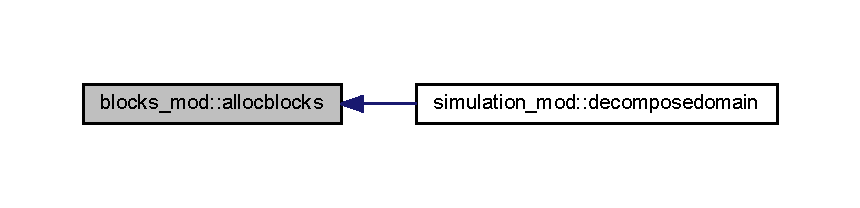
\includegraphics[width=350pt]{namespaceblocks__mod_a639beb0fee2290d46353f4b4702d6711_icgraph}
\end{center}
\end{figure}
\mbox{\Hypertarget{namespaceblocks__mod_a27c7e788c5f3979bfe9d43aad138286a}\label{namespaceblocks__mod_a27c7e788c5f3979bfe9d43aad138286a}} 
\index{blocks\+\_\+mod@{blocks\+\_\+mod}!aottotracers@{aottotracers}}
\index{aottotracers@{aottotracers}!blocks\+\_\+mod@{blocks\+\_\+mod}}
\subsubsection{\texorpdfstring{aottotracers()}{aottotracers()}}
{\footnotesize\ttfamily subroutine blocks\+\_\+mod\+::aottotracers (\begin{DoxyParamCaption}\item[{class(\mbox{\hyperlink{structblocks__mod_1_1block__class}{block\+\_\+class}}), intent(inout)}]{self }\end{DoxyParamCaption})\hspace{0.3cm}{\ttfamily [private]}}



Method to write the data in the AoT back to the Tracer objects in the list. 

\begin{DoxyAuthor}{Author}
Ricardo Birjukovs Canelas -\/ M\+A\+R\+E\+T\+EC 
\end{DoxyAuthor}


Definition at line 305 of file blocks.\+f90.


\begin{DoxyCode}
305     \textcolor{keywordtype}{implicit none}
306     \textcolor{keywordtype}{class}(block\_class), \textcolor{keywordtype}{intent(inout)} :: self
307     \textcolor{keyword}{call }self%AoT%toTracers()
\end{DoxyCode}
\mbox{\Hypertarget{namespaceblocks__mod_a2c3cf5113e1422d812c2c869afde2729}\label{namespaceblocks__mod_a2c3cf5113e1422d812c2c869afde2729}} 
\index{blocks\+\_\+mod@{blocks\+\_\+mod}!callemitter@{callemitter}}
\index{callemitter@{callemitter}!blocks\+\_\+mod@{blocks\+\_\+mod}}
\subsubsection{\texorpdfstring{callemitter()}{callemitter()}}
{\footnotesize\ttfamily subroutine blocks\+\_\+mod\+::callemitter (\begin{DoxyParamCaption}\item[{class(\mbox{\hyperlink{structblocks__mod_1_1block__class}{block\+\_\+class}}), intent(inout)}]{self }\end{DoxyParamCaption})\hspace{0.3cm}{\ttfamily [private]}}



Method to emitt Tracers from currently active Sources on the Block. 

\begin{DoxyAuthor}{Author}
Ricardo Birjukovs Canelas -\/ M\+A\+R\+E\+T\+EC 
\end{DoxyAuthor}


Definition at line 170 of file blocks.\+f90.


\begin{DoxyCode}
170     \textcolor{keywordtype}{implicit none}
171     \textcolor{keywordtype}{class}(block\_class), \textcolor{keywordtype}{intent(inout)} :: self
172     \textcolor{keywordtype}{integer} :: i
173     \textcolor{keywordtype}{class}(*), \textcolor{keywordtype}{pointer} :: aSource
174     \textcolor{keywordtype}{type}(string) :: outext
175     
176     \textcolor{keyword}{call }self%LSource%reset()                   \textcolor{comment}{! reset list iterator}
177     \textcolor{keywordflow}{do} \textcolor{keywordflow}{while}(self%LSource%moreValues())         \textcolor{comment}{! loop while there are values}
178         asource => self%LSource%currentValue()  \textcolor{comment}{! get current value}
179         \textcolor{keywordflow}{select type}(asource)
180 \textcolor{keywordflow}{        class is} (source\_class)
181             \textcolor{keywordflow}{if} (asource%now%active) \textcolor{keywordflow}{then}
182                 asource%now%emission\_stride = asource%now%emission\_stride - 1   \textcolor{comment}{!decreasing the stride at
       this dt}
183                 \textcolor{keywordflow}{if} (asource%now%emission\_stride == 0) \textcolor{keywordflow}{then}                      \textcolor{comment}{!reached the bottom of the
       stride stack, time to emitt}
184                     \textcolor{keyword}{call }self%Emitter%emitt(asource, self%LTracer)
185                     asource%now%emission\_stride = asource%par%emitting\_rate     \textcolor{comment}{!reseting the stride after
       the Source emitts}
186 \textcolor{keywordflow}{                end if}
187 \textcolor{keywordflow}{            end if}
188 \textcolor{keywordflow}{            class default}
189             outext = \textcolor{stringliteral}{'[Block::CallEmitter] Unexepected type of content, not a Source'}
190             \textcolor{keyword}{call }log%put(outext)
191             stop
192 \textcolor{keywordflow}{        end select}
193         \textcolor{keyword}{call }self%LSource%next()            \textcolor{comment}{! increment the list iterator}
194 \textcolor{keywordflow}{    end do}
195     \textcolor{keyword}{call }self%LSource%reset()               \textcolor{comment}{! reset list iterator}
196     
\end{DoxyCode}
\mbox{\Hypertarget{namespaceblocks__mod_a6cc313e046daa2720cbca810d083faa0}\label{namespaceblocks__mod_a6cc313e046daa2720cbca810d083faa0}} 
\index{blocks\+\_\+mod@{blocks\+\_\+mod}!cleanaot@{cleanaot}}
\index{cleanaot@{cleanaot}!blocks\+\_\+mod@{blocks\+\_\+mod}}
\subsubsection{\texorpdfstring{cleanaot()}{cleanaot()}}
{\footnotesize\ttfamily subroutine blocks\+\_\+mod\+::cleanaot (\begin{DoxyParamCaption}\item[{class(\mbox{\hyperlink{structblocks__mod_1_1block__class}{block\+\_\+class}}), intent(inout)}]{self }\end{DoxyParamCaption})\hspace{0.3cm}{\ttfamily [private]}}



Method to clean out the AoT object. 

\begin{DoxyAuthor}{Author}
Ricardo Birjukovs Canelas -\/ M\+A\+R\+E\+T\+EC 
\end{DoxyAuthor}


Definition at line 316 of file blocks.\+f90.


\begin{DoxyCode}
316     \textcolor{keywordtype}{implicit none}
317     \textcolor{keywordtype}{class}(block\_class), \textcolor{keywordtype}{intent(inout)} :: self    
318     \textcolor{keyword}{call }self%AoT%Clean()
\end{DoxyCode}
\mbox{\Hypertarget{namespaceblocks__mod_a25ff530b5125e4cee5b1f474b2491883}\label{namespaceblocks__mod_a25ff530b5125e4cee5b1f474b2491883}} 
\index{blocks\+\_\+mod@{blocks\+\_\+mod}!consolidatearrays@{consolidatearrays}}
\index{consolidatearrays@{consolidatearrays}!blocks\+\_\+mod@{blocks\+\_\+mod}}
\subsubsection{\texorpdfstring{consolidatearrays()}{consolidatearrays()}}
{\footnotesize\ttfamily subroutine blocks\+\_\+mod\+::consolidatearrays (\begin{DoxyParamCaption}\item[{class(\mbox{\hyperlink{structblocks__mod_1_1block__class}{block\+\_\+class}}), intent(inout)}]{self }\end{DoxyParamCaption})\hspace{0.3cm}{\ttfamily [private]}}



Method to clean the Tracer list from inactive Tracers. T\+O\+DO test further optimization. 

\begin{DoxyAuthor}{Author}
Ricardo Birjukovs Canelas -\/ M\+A\+R\+E\+T\+EC 
\end{DoxyAuthor}


Definition at line 245 of file blocks.\+f90.


\begin{DoxyCode}
245     \textcolor{keywordtype}{implicit none}
246     \textcolor{keywordtype}{class}(block\_class), \textcolor{keywordtype}{intent(inout)} :: self
247     \textcolor{keywordtype}{class}(*), \textcolor{keywordtype}{pointer} :: aTracer
248     \textcolor{keywordtype}{type}(string) :: outext
249     \textcolor{keywordtype}{logical} :: notremoved
250     
251     \textcolor{keyword}{call }self%LTracer%reset()                   \textcolor{comment}{! reset list iterator}
252     \textcolor{keywordflow}{do} \textcolor{keywordflow}{while}(self%LTracer%moreValues())         \textcolor{comment}{! loop while there are values}
253         notremoved = .true.
254         atracer => self%LTracer%currentValue()  \textcolor{comment}{! get current value}
255         \textcolor{keywordflow}{select type}(atracer)
256 \textcolor{keywordflow}{        class is} (tracer\_class)
257             \textcolor{keywordflow}{if} (atracer%now%active.eqv. .false.) \textcolor{keywordflow}{then}
258                 \textcolor{keyword}{call }self%LTracer%removeCurrent() \textcolor{comment}{!this advances the iterator to the next position}
259                 notremoved = .false.                
260 \textcolor{keywordflow}{            end if}
261 \textcolor{keywordflow}{            class default}
262             outext = \textcolor{stringliteral}{'[Block::ConsolidateArrays]: Unexepected type of content, not a Tracer'}
263             \textcolor{keyword}{call }log%put(outext)
264             stop
265 \textcolor{keywordflow}{        end select}
266         \textcolor{keywordflow}{if} (notremoved) \textcolor{keyword}{call }self%LTracer%next()    \textcolor{comment}{! increment the list iterator}
267 \textcolor{keywordflow}{    end do}
268     \textcolor{keyword}{call }self%LTracer%reset()                       \textcolor{comment}{! reset list iterator}
269     
\end{DoxyCode}
\mbox{\Hypertarget{namespaceblocks__mod_aa178415bcc40cf169744d356e1a09c6b}\label{namespaceblocks__mod_aa178415bcc40cf169744d356e1a09c6b}} 
\index{blocks\+\_\+mod@{blocks\+\_\+mod}!distributetracers@{distributetracers}}
\index{distributetracers@{distributetracers}!blocks\+\_\+mod@{blocks\+\_\+mod}}
\subsubsection{\texorpdfstring{distributetracers()}{distributetracers()}}
{\footnotesize\ttfamily subroutine blocks\+\_\+mod\+::distributetracers (\begin{DoxyParamCaption}\item[{class(\mbox{\hyperlink{structblocks__mod_1_1block__class}{block\+\_\+class}}), intent(inout)}]{self }\end{DoxyParamCaption})\hspace{0.3cm}{\ttfamily [private]}}



Method to distribute the Tracers to their correct Blocks. 

\begin{DoxyAuthor}{Author}
Ricardo Birjukovs Canelas -\/ M\+A\+R\+E\+T\+EC 
\end{DoxyAuthor}


Definition at line 205 of file blocks.\+f90.


\begin{DoxyCode}
205     \textcolor{keywordtype}{implicit none}
206     \textcolor{keywordtype}{class}(block\_class), \textcolor{keywordtype}{intent(inout)} :: self
207     \textcolor{keywordtype}{integer} :: i, blk
208     \textcolor{keywordtype}{class}(*), \textcolor{keywordtype}{pointer} :: aTracer
209     \textcolor{keywordtype}{type}(string) :: outext
210     \textcolor{keywordtype}{logical} :: notremoved
211     
212     \textcolor{keyword}{call }self%LTracer%reset()                   \textcolor{comment}{! reset list iterator}
213     \textcolor{keywordflow}{do} \textcolor{keywordflow}{while}(self%LTracer%moreValues())         \textcolor{comment}{! loop while there are values}
214         notremoved = .true.
215         atracer => self%LTracer%currentValue()  \textcolor{comment}{! get current value}
216         \textcolor{keywordflow}{select type}(atracer)
217 \textcolor{keywordflow}{        class is} (tracer\_class)
218             \textcolor{keywordflow}{if} (atracer%now%active) \textcolor{keywordflow}{then}
219                 blk = getblockindex(atracer%now%pos)
220                 \textcolor{keywordflow}{if} (blk /= self%id) \textcolor{keywordflow}{then}        \textcolor{comment}{!tracer is on a different block than the current one}
221                     \textcolor{comment}{!PARALLEL this is a CRITICAL section, need to ensure correct tracer index attribution}
222                     \textcolor{keyword}{call }sendtracer(blk,atracer)
223                     \textcolor{keyword}{call }self%LTracer%removeCurrent() \textcolor{comment}{!this also advances the iterator to the next position}
224                     notremoved = .false.
225 \textcolor{keywordflow}{                end if}
226 \textcolor{keywordflow}{            end if}
227 \textcolor{keywordflow}{            class default}
228             outext = \textcolor{stringliteral}{'[Block::DistributeTracers]: Unexepected type of content, not a Tracer'}
229             \textcolor{keyword}{call }log%put(outext)
230             stop
231 \textcolor{keywordflow}{        end select}
232         \textcolor{keywordflow}{if} (notremoved) \textcolor{keyword}{call }self%LTracer%next()    \textcolor{comment}{! increment the list iterator}
233 \textcolor{keywordflow}{    end do}
234     \textcolor{keyword}{call }self%LTracer%reset()                   \textcolor{comment}{! reset list iterator}
235     
\end{DoxyCode}
Here is the call graph for this function\+:\nopagebreak
\begin{figure}[H]
\begin{center}
\leavevmode
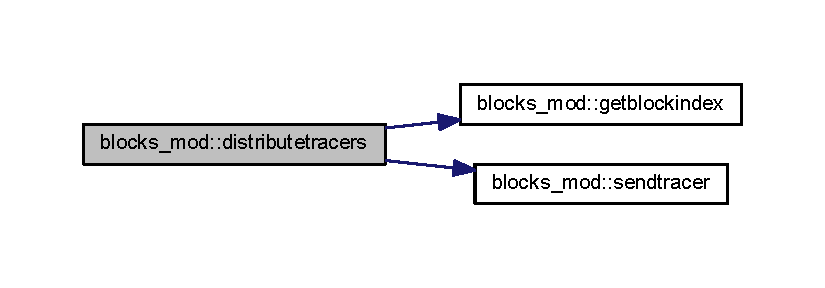
\includegraphics[width=350pt]{namespaceblocks__mod_aa178415bcc40cf169744d356e1a09c6b_cgraph}
\end{center}
\end{figure}
\mbox{\Hypertarget{namespaceblocks__mod_a62e8fb0d6b2535b4499c7a4d848c24ba}\label{namespaceblocks__mod_a62e8fb0d6b2535b4499c7a4d848c24ba}} 
\index{blocks\+\_\+mod@{blocks\+\_\+mod}!getblockindex@{getblockindex}}
\index{getblockindex@{getblockindex}!blocks\+\_\+mod@{blocks\+\_\+mod}}
\subsubsection{\texorpdfstring{getblockindex()}{getblockindex()}}
{\footnotesize\ttfamily integer function, public blocks\+\_\+mod\+::getblockindex (\begin{DoxyParamCaption}\item[{type(vector), intent(in)}]{pt }\end{DoxyParamCaption})}



Returns the index of a Block for a given set of coordinates. 

\begin{DoxyAuthor}{Author}
Ricardo Birjukovs Canelas -\/ M\+A\+R\+E\+T\+EC 
\end{DoxyAuthor}

\begin{DoxyParams}[1]{Parameters}
\mbox{\tt in}  & {\em pt} & \\
\hline
\end{DoxyParams}


Definition at line 342 of file blocks.\+f90.


\begin{DoxyCode}
342     \textcolor{keywordtype}{implicit none}
343     \textcolor{keywordtype}{type}(vector), \textcolor{keywordtype}{intent(in)} :: pt
344     \textcolor{keywordtype}{integer} :: ix, iy, temp
345     \textcolor{keywordtype}{type}(string) :: outext
346     ix = min(int((pt%x + bbox%offset%x)/globals%SimDefs%blocksize%x) + 1, globals%SimDefs%numblocksx)
347     iy = min(int((pt%y + bbox%offset%y)/globals%SimDefs%blocksize%y) + 1, globals%SimDefs%numblocksy)
348     temp = 2*ix + iy -2
349     \textcolor{keywordflow}{if} (temp > globals%SimDefs%numblocks) \textcolor{keywordflow}{then}
350         outext=\textcolor{stringliteral}{'[Blocks::getBlockIndex]: problem in getting correct Block index, stoping'}
351         \textcolor{keyword}{call }log%put(outext)
352         stop
353 \textcolor{keywordflow}{    end if}
354     getblockindex = temp
\end{DoxyCode}
Here is the caller graph for this function\+:\nopagebreak
\begin{figure}[H]
\begin{center}
\leavevmode
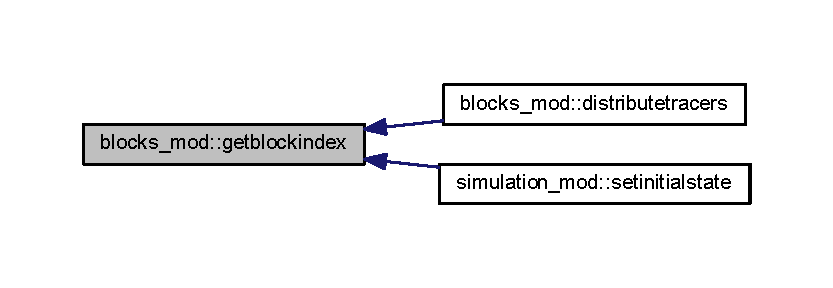
\includegraphics[width=350pt]{namespaceblocks__mod_a62e8fb0d6b2535b4499c7a4d848c24ba_icgraph}
\end{center}
\end{figure}
\mbox{\Hypertarget{namespaceblocks__mod_a534ca69b17b6f54ee07f995b02feff39}\label{namespaceblocks__mod_a534ca69b17b6f54ee07f995b02feff39}} 
\index{blocks\+\_\+mod@{blocks\+\_\+mod}!initblock@{initblock}}
\index{initblock@{initblock}!blocks\+\_\+mod@{blocks\+\_\+mod}}
\subsubsection{\texorpdfstring{initblock()}{initblock()}}
{\footnotesize\ttfamily subroutine blocks\+\_\+mod\+::initblock (\begin{DoxyParamCaption}\item[{class(\mbox{\hyperlink{structblocks__mod_1_1block__class}{block\+\_\+class}}), intent(inout)}]{self,  }\item[{integer, intent(in)}]{id,  }\item[{type(\mbox{\hyperlink{structgeometry__mod_1_1box}{box}}), intent(in)}]{templatebox }\end{DoxyParamCaption})\hspace{0.3cm}{\ttfamily [private]}}



method to allocate and initialize Blocks and their Emitters 

\begin{DoxyAuthor}{Author}
Ricardo Birjukovs Canelas -\/ M\+A\+R\+E\+T\+EC 
\end{DoxyAuthor}

\begin{DoxyParams}[1]{Parameters}
\mbox{\tt in}  & {\em self,id,templatebox} & \\
\hline
\end{DoxyParams}


Definition at line 95 of file blocks.\+f90.


\begin{DoxyCode}
95     \textcolor{keywordtype}{implicit none}
96     \textcolor{keywordtype}{class}(block\_class), \textcolor{keywordtype}{intent(inout)} :: self
97     \textcolor{keywordtype}{integer}, \textcolor{keywordtype}{intent(in)} :: id
98     \textcolor{keywordtype}{type}(box), \textcolor{keywordtype}{intent(in)} :: templatebox
99     \textcolor{keywordtype}{integer} :: sizem, i
100     self%id = id
101     \textcolor{comment}{!setting the block sub-domain}
102     self%extents = templatebox
103     \textcolor{comment}{!initializing the block emitter}
104     \textcolor{keyword}{call }self%Emitter%initialize()
105     \textcolor{comment}{!initializing the block solver}
106     i = globals%Parameters%Integrator
107     \textcolor{keyword}{call }self%Solver%initialize(i, globals%Parameters%IntegratorNames(i))
108     sizem = sizeof(self)
109     \textcolor{keyword}{call }simmemory%addblock(sizem)
\end{DoxyCode}
\mbox{\Hypertarget{namespaceblocks__mod_a7202fad0fdc07ff9111e61e3aa513af9}\label{namespaceblocks__mod_a7202fad0fdc07ff9111e61e3aa513af9}} 
\index{blocks\+\_\+mod@{blocks\+\_\+mod}!numalloctracers@{numalloctracers}}
\index{numalloctracers@{numalloctracers}!blocks\+\_\+mod@{blocks\+\_\+mod}}
\subsubsection{\texorpdfstring{numalloctracers()}{numalloctracers()}}
{\footnotesize\ttfamily integer function blocks\+\_\+mod\+::numalloctracers (\begin{DoxyParamCaption}\item[{class(\mbox{\hyperlink{structblocks__mod_1_1block__class}{block\+\_\+class}}), intent(in)}]{self }\end{DoxyParamCaption})\hspace{0.3cm}{\ttfamily [private]}}



method that returns the total allocated Tracers in the Block 

\begin{DoxyAuthor}{Author}
Ricardo Birjukovs Canelas -\/ M\+A\+R\+E\+T\+EC 
\end{DoxyAuthor}


Definition at line 82 of file blocks.\+f90.


\begin{DoxyCode}
82     \textcolor{keywordtype}{implicit none}
83     \textcolor{keywordtype}{class}(block\_class), \textcolor{keywordtype}{intent(in)} :: self
84     \textcolor{keywordtype}{integer} :: numAllocTracers
85     numalloctracers = self%LTracer%getSize()
\end{DoxyCode}
\mbox{\Hypertarget{namespaceblocks__mod_a6eab8b323cb15dcecb5c6b0c31b4e246}\label{namespaceblocks__mod_a6eab8b323cb15dcecb5c6b0c31b4e246}} 
\index{blocks\+\_\+mod@{blocks\+\_\+mod}!printblock@{printblock}}
\index{printblock@{printblock}!blocks\+\_\+mod@{blocks\+\_\+mod}}
\subsubsection{\texorpdfstring{printblock()}{printblock()}}
{\footnotesize\ttfamily subroutine blocks\+\_\+mod\+::printblock (\begin{DoxyParamCaption}\item[{class(\mbox{\hyperlink{structblocks__mod_1_1block__class}{block\+\_\+class}}), intent(inout)}]{self }\end{DoxyParamCaption})\hspace{0.3cm}{\ttfamily [private]}}



Method to print basic info about the block. 

\begin{DoxyAuthor}{Author}
Ricardo Birjukovs Canelas -\/ M\+A\+R\+E\+T\+EC 
\end{DoxyAuthor}

\begin{DoxyParams}[1]{Parameters}
\mbox{\tt in}  & {\em self} & \\
\hline
\end{DoxyParams}


Definition at line 364 of file blocks.\+f90.


\begin{DoxyCode}
364     \textcolor{keywordtype}{implicit none}
365     \textcolor{keywordtype}{class}(block\_class), \textcolor{keywordtype}{intent(inout)} :: self
366     \textcolor{keywordtype}{type}(string) :: outext, temp\_str
367     temp\_str = self%id
368     outext=\textcolor{stringliteral}{'-->Block '}//temp\_str//\textcolor{stringliteral}{' is a'}
369     \textcolor{keyword}{call }log%put(outext,.false.)
370     \textcolor{keyword}{call }geometry%print(self%extents)
371     temp\_str = self%LSource%getSize()
372     outext=\textcolor{stringliteral}{'      and has '}//temp\_str//\textcolor{stringliteral}{' Sources'}
373     \textcolor{keyword}{call }log%put(outext,.false.)
\end{DoxyCode}
\mbox{\Hypertarget{namespaceblocks__mod_a10f356706988c45a255922fe70851488}\label{namespaceblocks__mod_a10f356706988c45a255922fe70851488}} 
\index{blocks\+\_\+mod@{blocks\+\_\+mod}!printdetailblock@{printdetailblock}}
\index{printdetailblock@{printdetailblock}!blocks\+\_\+mod@{blocks\+\_\+mod}}
\subsubsection{\texorpdfstring{printdetailblock()}{printdetailblock()}}
{\footnotesize\ttfamily subroutine blocks\+\_\+mod\+::printdetailblock (\begin{DoxyParamCaption}\item[{class(\mbox{\hyperlink{structblocks__mod_1_1block__class}{block\+\_\+class}}), intent(inout)}]{self }\end{DoxyParamCaption})\hspace{0.3cm}{\ttfamily [private]}}



Method to print detailed info about the block. 

\begin{DoxyAuthor}{Author}
Ricardo Birjukovs Canelas -\/ M\+A\+R\+E\+T\+EC 
\end{DoxyAuthor}

\begin{DoxyParams}[1]{Parameters}
\mbox{\tt in}  & {\em self} & \\
\hline
\end{DoxyParams}


Definition at line 383 of file blocks.\+f90.


\begin{DoxyCode}
383     \textcolor{keywordtype}{implicit none}
384     \textcolor{keywordtype}{class}(block\_class), \textcolor{keywordtype}{intent(inout)} :: self
385     \textcolor{keywordtype}{type}(string) :: outext, temp\_str
386     \textcolor{keywordtype}{integer} :: i
387     temp\_str = self%id
388     outext=\textcolor{stringliteral}{'-->Block '}//temp\_str//\textcolor{stringliteral}{' is a'}
389     \textcolor{keyword}{call }log%put(outext,.false.)
390     \textcolor{keyword}{call }geometry%print(self%extents)
391     temp\_str = self%LSource%getSize()
392     outext=\textcolor{stringliteral}{'      and has '}//temp\_str//\textcolor{stringliteral}{' Sources'}
393     \textcolor{keyword}{call }log%put(outext,.false.)
394     \textcolor{keyword}{call }self%LSource%print()
\end{DoxyCode}
\mbox{\Hypertarget{namespaceblocks__mod_ae3bd1bfeee831f4b41932839495bb108}\label{namespaceblocks__mod_ae3bd1bfeee831f4b41932839495bb108}} 
\index{blocks\+\_\+mod@{blocks\+\_\+mod}!putsource@{putsource}}
\index{putsource@{putsource}!blocks\+\_\+mod@{blocks\+\_\+mod}}
\subsubsection{\texorpdfstring{putsource()}{putsource()}}
{\footnotesize\ttfamily subroutine blocks\+\_\+mod\+::putsource (\begin{DoxyParamCaption}\item[{class(\mbox{\hyperlink{structblocks__mod_1_1block__class}{block\+\_\+class}}), intent(inout)}]{self,  }\item[{class(\mbox{\hyperlink{structsources__mod_1_1source__class}{source\+\_\+class}}), intent(inout)}]{sourcetoadd }\end{DoxyParamCaption})\hspace{0.3cm}{\ttfamily [private]}}



Method to place a Source on the Block source\+List\+\_\+class object. Adds the Source info to the Block Emitter. 

\begin{DoxyAuthor}{Author}
Ricardo Birjukovs Canelas -\/ M\+A\+R\+E\+T\+EC 
\end{DoxyAuthor}

\begin{DoxyParams}[1]{Parameters}
\mbox{\tt in}  & {\em self,sourcetoadd} & \\
\hline
\mbox{\tt in,out}  & {\em sourcetoadd} & Source object to store \\
\hline
\end{DoxyParams}


Definition at line 120 of file blocks.\+f90.


\begin{DoxyCode}
120     \textcolor{keywordtype}{implicit none}
121     \textcolor{keywordtype}{class}(block\_class), \textcolor{keywordtype}{intent(inout)} :: self
122     \textcolor{keywordtype}{class}(source\_class), \textcolor{keywordtype}{intent(inout)} :: sourcetoadd
123     \textcolor{keyword}{call }self%LSource%add(sourcetoadd)    
124     \textcolor{comment}{!adding this Source to the Block Emitter pool}
125     \textcolor{keyword}{call }self%Emitter%addSource(sourcetoadd)
\end{DoxyCode}
\mbox{\Hypertarget{namespaceblocks__mod_a3245bdadbec6bb123c517921d1503b48}\label{namespaceblocks__mod_a3245bdadbec6bb123c517921d1503b48}} 
\index{blocks\+\_\+mod@{blocks\+\_\+mod}!runsolver@{runsolver}}
\index{runsolver@{runsolver}!blocks\+\_\+mod@{blocks\+\_\+mod}}
\subsubsection{\texorpdfstring{runsolver()}{runsolver()}}
{\footnotesize\ttfamily subroutine blocks\+\_\+mod\+::runsolver (\begin{DoxyParamCaption}\item[{class(\mbox{\hyperlink{structblocks__mod_1_1block__class}{block\+\_\+class}}), intent(inout)}]{self }\end{DoxyParamCaption})\hspace{0.3cm}{\ttfamily [private]}}



Method to run the solver on the data on this Block for the current timestep. Time for some actual numerical work! 

\begin{DoxyAuthor}{Author}
Ricardo Birjukovs Canelas -\/ M\+A\+R\+E\+T\+EC 
\end{DoxyAuthor}


Definition at line 294 of file blocks.\+f90.


\begin{DoxyCode}
294     \textcolor{keywordtype}{implicit none}
295     \textcolor{keywordtype}{class}(block\_class), \textcolor{keywordtype}{intent(inout)} :: self
296     \textcolor{keyword}{call }self%Solver%runStep(self%AoT, self%Background, globals%SimTime, globals%SimDefs%dt)
\end{DoxyCode}
\mbox{\Hypertarget{namespaceblocks__mod_a5a9992de40470e417ec8e40e688f6a0e}\label{namespaceblocks__mod_a5a9992de40470e417ec8e40e688f6a0e}} 
\index{blocks\+\_\+mod@{blocks\+\_\+mod}!sendtracer@{sendtracer}}
\index{sendtracer@{sendtracer}!blocks\+\_\+mod@{blocks\+\_\+mod}}
\subsubsection{\texorpdfstring{sendtracer()}{sendtracer()}}
{\footnotesize\ttfamily subroutine blocks\+\_\+mod\+::sendtracer (\begin{DoxyParamCaption}\item[{integer, intent(in)}]{blk,  }\item[{class($\ast$), intent(in)}]{trc }\end{DoxyParamCaption})\hspace{0.3cm}{\ttfamily [private]}}



Method to send a Tracer from the current Block to another Block. 

\begin{DoxyAuthor}{Author}
Ricardo Birjukovs Canelas -\/ M\+A\+R\+E\+T\+EC 
\end{DoxyAuthor}


Definition at line 327 of file blocks.\+f90.


\begin{DoxyCode}
327     \textcolor{keywordtype}{implicit none}
328     \textcolor{keywordtype}{integer}, \textcolor{keywordtype}{intent(in)} :: blk
329     \textcolor{keywordtype}{class}(*), \textcolor{keywordtype}{intent(in)} :: trc
330     \textcolor{comment}{!PARALLEL this is a CRITICAL section, need to ensure correct tracer}
331     \textcolor{comment}{!index attribution at the new block}
332     \textcolor{keyword}{call }dblock(blk)%LTracer%add(trc)
\end{DoxyCode}
Here is the caller graph for this function\+:\nopagebreak
\begin{figure}[H]
\begin{center}
\leavevmode
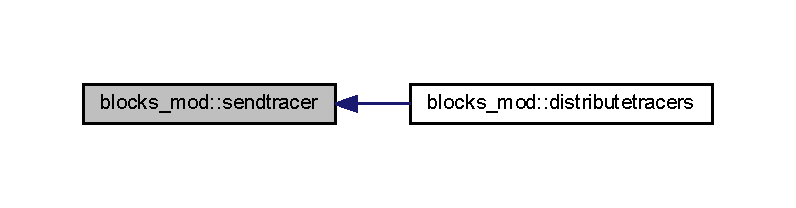
\includegraphics[width=350pt]{namespaceblocks__mod_a5a9992de40470e417ec8e40e688f6a0e_icgraph}
\end{center}
\end{figure}
\mbox{\Hypertarget{namespaceblocks__mod_a8f5a5d9e6cfd16cfd1b179092a204696}\label{namespaceblocks__mod_a8f5a5d9e6cfd16cfd1b179092a204696}} 
\index{blocks\+\_\+mod@{blocks\+\_\+mod}!setblocks@{setblocks}}
\index{setblocks@{setblocks}!blocks\+\_\+mod@{blocks\+\_\+mod}}
\subsubsection{\texorpdfstring{setblocks()}{setblocks()}}
{\footnotesize\ttfamily subroutine, public blocks\+\_\+mod\+::setblocks (\begin{DoxyParamCaption}\item[{logical, intent(in)}]{auto,  }\item[{integer, intent(in)}]{nblk,  }\item[{integer, intent(out)}]{nxi,  }\item[{integer, intent(out)}]{nyi }\end{DoxyParamCaption})}



routine to set the simulation blocks extents and call the block initializer 

\begin{DoxyAuthor}{Author}
Ricardo Birjukovs Canelas -\/ M\+A\+R\+E\+T\+EC 
\end{DoxyAuthor}

\begin{DoxyParams}[1]{Parameters}
\mbox{\tt in}  & {\em auto,nblk,nxi,nyi} & \\
\hline
\end{DoxyParams}


Definition at line 404 of file blocks.\+f90.


\begin{DoxyCode}
404     \textcolor{keywordtype}{implicit none}
405     \textcolor{keywordtype}{logical}, \textcolor{keywordtype}{intent(in)} ::  auto
406     \textcolor{keywordtype}{integer}, \textcolor{keywordtype}{intent(in)} ::  nblk
407     \textcolor{keywordtype}{integer}, \textcolor{keywordtype}{intent(out)} :: nxi, nyi
408     \textcolor{keywordtype}{type}(string) :: outext, temp(2)
409     \textcolor{keywordtype}{integer} :: i, j, b
410     \textcolor{keywordtype}{real(prec)} :: ar
411     \textcolor{keywordtype}{type}(box) :: tempbox
412 
413     \textcolor{keywordflow}{if} (auto) \textcolor{keywordflow}{then}
414         ar = bbox%size%x/bbox%size%y
415         ar = get\_closest\_twopow(ar) \textcolor{comment}{!aspect ratio of our bounding box}
416         nyi = sqrt(nblk/ar)
417         \textcolor{keywordflow}{if} (nyi == 0) \textcolor{keywordflow}{then}
418             temp(1) = ar
419             outext=\textcolor{stringliteral}{'[setBlocks]: block auto sizing failed. Bouding box aspect ratio = '}//temp(1)//\textcolor{stringliteral}{'.
       Stoping'}
420             \textcolor{keyword}{call }log%put(outext)
421             stop
422 \textcolor{keywordflow}{        endif}
423         nxi = (nblk/nyi)
424 
425         b=1
426         \textcolor{keywordflow}{do} i=1, nxi
427             \textcolor{keywordflow}{do} j=1, nyi
428                 tempbox%pt = bbox%pt + bbox%size%x*(i-1)/nxi*ex + bbox%size%y*(j-1)/nyi*ey - bbox%pt%z*ez
429                 tempbox%size = bbox%size%x/nxi*ex + bbox%size%y/nyi*ey
430                 \textcolor{keyword}{call }dblock(b)%initialize(b, tempbox)
431                 b=b+1
432 \textcolor{keywordflow}{            end do}
433 \textcolor{keywordflow}{        end do}
434         temp(1) = nxi
435         temp(2) = nyi
436         outext=\textcolor{stringliteral}{'-->Automatic domain decomposition sucessful. Domain is '}//temp(1)// \textcolor{stringliteral}{' X '} //temp(2)//\textcolor{stringliteral}{'
       Blocks'}
437         \textcolor{keyword}{call }log%put(outext,.false.)
438 \textcolor{keywordflow}{    end if}
439     globals%SimDefs%blocksize = dblock(1)%extents%size
440     \textcolor{comment}{!do i=1, size(DBlock)}
441     \textcolor{comment}{!    call DBlock(i)%print()}
442     \textcolor{comment}{!enddo}
443 
444     \textcolor{keywordflow}{return}
\end{DoxyCode}
Here is the caller graph for this function\+:\nopagebreak
\begin{figure}[H]
\begin{center}
\leavevmode
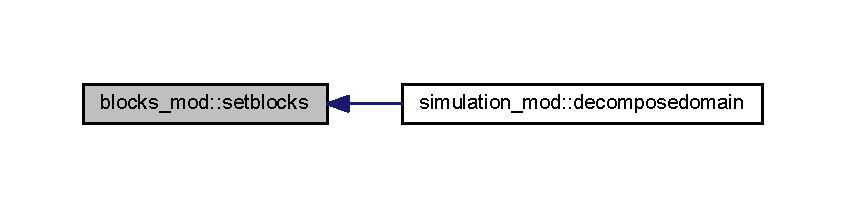
\includegraphics[width=350pt]{namespaceblocks__mod_a8f5a5d9e6cfd16cfd1b179092a204696_icgraph}
\end{center}
\end{figure}
\mbox{\Hypertarget{namespaceblocks__mod_ab9e57cbf0103b632b2b2dfa4e4d4139c}\label{namespaceblocks__mod_ab9e57cbf0103b632b2b2dfa4e4d4139c}} 
\index{blocks\+\_\+mod@{blocks\+\_\+mod}!toogleblocksources@{toogleblocksources}}
\index{toogleblocksources@{toogleblocksources}!blocks\+\_\+mod@{blocks\+\_\+mod}}
\subsubsection{\texorpdfstring{toogleblocksources()}{toogleblocksources()}}
{\footnotesize\ttfamily subroutine blocks\+\_\+mod\+::toogleblocksources (\begin{DoxyParamCaption}\item[{class(\mbox{\hyperlink{structblocks__mod_1_1block__class}{block\+\_\+class}}), intent(inout)}]{self }\end{DoxyParamCaption})\hspace{0.3cm}{\ttfamily [private]}}



Method to activate and deactivate the sources on this block, based on GlobaSim\+Time. 

\begin{DoxyAuthor}{Author}
Ricardo Birjukovs Canelas -\/ M\+A\+R\+E\+T\+EC 
\end{DoxyAuthor}


Definition at line 135 of file blocks.\+f90.


\begin{DoxyCode}
135     \textcolor{keywordtype}{implicit none}
136     \textcolor{keywordtype}{class}(block\_class), \textcolor{keywordtype}{intent(inout)} :: self
137     \textcolor{keywordtype}{integer} :: i
138     \textcolor{keywordtype}{class}(*), \textcolor{keywordtype}{pointer} :: aSource
139     \textcolor{keywordtype}{type}(string) :: outext
140 
141     \textcolor{keyword}{call }self%LSource%reset()                   \textcolor{comment}{! reset list iterator}
142     \textcolor{keywordflow}{do} \textcolor{keywordflow}{while}(self%LSource%moreValues())         \textcolor{comment}{! loop while there are values}
143         asource => self%LSource%currentValue()  \textcolor{comment}{! get current value}
144         \textcolor{keywordflow}{select type}(asource)
145 \textcolor{keywordflow}{        class is} (source\_class)
146             \textcolor{keywordflow}{if} (globals%SimTime <= asource%par%stoptime) \textcolor{keywordflow}{then}       \textcolor{comment}{!SimTime smaller than Source end time}
147                 \textcolor{keywordflow}{if} (globals%SimTime >= asource%par%startime) \textcolor{keywordflow}{then}   \textcolor{comment}{!SimTime larger than source start time}
148                     asource%now%active = .true.
149 \textcolor{keywordflow}{                end if}
150             \textcolor{keywordflow}{else}            \textcolor{comment}{!SimTime larger than Source end time}
151                 asource%now%active = .false.
152 \textcolor{keywordflow}{            end if}
153 \textcolor{keywordflow}{            class default}
154             outext = \textcolor{stringliteral}{'[Block::ToogleBlockSources] Unexepected type of content, not a Source'}
155             \textcolor{keyword}{call }log%put(outext)
156             stop
157 \textcolor{keywordflow}{        end select}
158         \textcolor{keyword}{call }self%LSource%next()            \textcolor{comment}{! increment the list iterator}
159 \textcolor{keywordflow}{    end do}
160     \textcolor{keyword}{call }self%LSource%reset()               \textcolor{comment}{! reset list iterator}
161 
\end{DoxyCode}
\mbox{\Hypertarget{namespaceblocks__mod_ae7afa742f8f89a6a8afdefb7f8c87efd}\label{namespaceblocks__mod_ae7afa742f8f89a6a8afdefb7f8c87efd}} 
\index{blocks\+\_\+mod@{blocks\+\_\+mod}!tracerstoaot@{tracerstoaot}}
\index{tracerstoaot@{tracerstoaot}!blocks\+\_\+mod@{blocks\+\_\+mod}}
\subsubsection{\texorpdfstring{tracerstoaot()}{tracerstoaot()}}
{\footnotesize\ttfamily subroutine blocks\+\_\+mod\+::tracerstoaot (\begin{DoxyParamCaption}\item[{class(\mbox{\hyperlink{structblocks__mod_1_1block__class}{block\+\_\+class}}), intent(inout)}]{self }\end{DoxyParamCaption})\hspace{0.3cm}{\ttfamily [private]}}



Method to build the AoT object at this timestep for actual numerical work. 

\begin{DoxyAuthor}{Author}
Ricardo Birjukovs Canelas -\/ M\+A\+R\+E\+T\+EC 
\end{DoxyAuthor}


Definition at line 278 of file blocks.\+f90.


\begin{DoxyCode}
278     \textcolor{keywordtype}{implicit none}
279     \textcolor{keywordtype}{class}(block\_class), \textcolor{keywordtype}{intent(inout)} :: self
280     self%AoT = aot(self%LTracer)
281     \textcolor{comment}{!if (self%LTracer%getSize() > 0) then}
282     \textcolor{comment}{!    print*, 'From Block ', self%id}
283     \textcolor{comment}{!    call self%AoT%print()}
284     \textcolor{comment}{!end if}
\end{DoxyCode}


\subsection{Variable Documentation}
\mbox{\Hypertarget{namespaceblocks__mod_ac8ad6e3cf7a812f95dadb592336aca50}\label{namespaceblocks__mod_ac8ad6e3cf7a812f95dadb592336aca50}} 
\index{blocks\+\_\+mod@{blocks\+\_\+mod}!dblock@{dblock}}
\index{dblock@{dblock}!blocks\+\_\+mod@{blocks\+\_\+mod}}
\subsubsection{\texorpdfstring{dblock}{dblock}}
{\footnotesize\ttfamily type(\mbox{\hyperlink{structblocks__mod_1_1block__class}{block\+\_\+class}}), dimension(\+:), allocatable, public blocks\+\_\+mod\+::dblock}



Definition at line 67 of file blocks.\+f90.


\begin{DoxyCode}
67     \textcolor{keywordtype}{type}(block\_class), \textcolor{keywordtype}{allocatable}, \textcolor{keywordtype}{dimension(:)} :: DBlock
\end{DoxyCode}

\hypertarget{namespaceboundingbox__mod}{}\section{boundingbox\+\_\+mod Module Reference}
\label{namespaceboundingbox__mod}\index{boundingbox\+\_\+mod@{boundingbox\+\_\+mod}}


Module that defines a simulation Bounding Box.  


\subsection*{Data Types}
\begin{DoxyCompactItemize}
\item 
type \hyperlink{structboundingbox__mod_1_1boundingbox__class}{boundingbox\+\_\+class}
\end{DoxyCompactItemize}
\subsection*{Functions/\+Subroutines}
\begin{DoxyCompactItemize}
\item 
subroutine \hyperlink{namespaceboundingbox__mod_a35e41bb92c19802441dd8d748c3acfb4}{initboundingbox} (self)
\begin{DoxyCompactList}\small\item\em Birjukovs Canelas -\/ M\+A\+R\+E\+T\+EC \end{DoxyCompactList}\item 
subroutine \hyperlink{namespaceboundingbox__mod_a6ec461b758bc180dc72b5fb23169feca}{printboundingbox} (self)
\begin{DoxyCompactList}\small\item\em Birjukovs Canelas -\/ M\+A\+R\+E\+T\+EC \end{DoxyCompactList}\end{DoxyCompactItemize}
\subsection*{Variables}
\begin{DoxyCompactItemize}
\item 
type(\hyperlink{structboundingbox__mod_1_1boundingbox__class}{boundingbox\+\_\+class}), public \hyperlink{namespaceboundingbox__mod_a45e98e492bb546328c98f618a74622ec}{bbox}
\end{DoxyCompactItemize}


\subsection{Detailed Description}
Module that defines a simulation Bounding Box. 

\begin{DoxyAuthor}{Author}
Ricardo Birjukovs Canelas 
\end{DoxyAuthor}


\subsection{Function/\+Subroutine Documentation}
\mbox{\Hypertarget{namespaceboundingbox__mod_a35e41bb92c19802441dd8d748c3acfb4}\label{namespaceboundingbox__mod_a35e41bb92c19802441dd8d748c3acfb4}} 
\index{boundingbox\+\_\+mod@{boundingbox\+\_\+mod}!initboundingbox@{initboundingbox}}
\index{initboundingbox@{initboundingbox}!boundingbox\+\_\+mod@{boundingbox\+\_\+mod}}
\subsubsection{\texorpdfstring{initboundingbox()}{initboundingbox()}}
{\footnotesize\ttfamily subroutine boundingbox\+\_\+mod\+::initboundingbox (\begin{DoxyParamCaption}\item[{class(\hyperlink{structboundingbox__mod_1_1boundingbox__class}{boundingbox\+\_\+class}), intent(inout)}]{self }\end{DoxyParamCaption})\hspace{0.3cm}{\ttfamily [private]}}



Birjukovs Canelas -\/ M\+A\+R\+E\+T\+EC 

Method to initialize the simulation Bounding Box \mbox{\Hypertarget{namespaceboundingbox__mod_a6ec461b758bc180dc72b5fb23169feca}\label{namespaceboundingbox__mod_a6ec461b758bc180dc72b5fb23169feca}} 
\index{boundingbox\+\_\+mod@{boundingbox\+\_\+mod}!printboundingbox@{printboundingbox}}
\index{printboundingbox@{printboundingbox}!boundingbox\+\_\+mod@{boundingbox\+\_\+mod}}
\subsubsection{\texorpdfstring{printboundingbox()}{printboundingbox()}}
{\footnotesize\ttfamily subroutine boundingbox\+\_\+mod\+::printboundingbox (\begin{DoxyParamCaption}\item[{class(\hyperlink{structboundingbox__mod_1_1boundingbox__class}{boundingbox\+\_\+class}), intent(inout)}]{self }\end{DoxyParamCaption})\hspace{0.3cm}{\ttfamily [private]}}



Birjukovs Canelas -\/ M\+A\+R\+E\+T\+EC 

Method to print the simulation Bounding Box 

\subsection{Variable Documentation}
\mbox{\Hypertarget{namespaceboundingbox__mod_a45e98e492bb546328c98f618a74622ec}\label{namespaceboundingbox__mod_a45e98e492bb546328c98f618a74622ec}} 
\index{boundingbox\+\_\+mod@{boundingbox\+\_\+mod}!bbox@{bbox}}
\index{bbox@{bbox}!boundingbox\+\_\+mod@{boundingbox\+\_\+mod}}
\subsubsection{\texorpdfstring{bbox}{bbox}}
{\footnotesize\ttfamily type(\hyperlink{structboundingbox__mod_1_1boundingbox__class}{boundingbox\+\_\+class}), public boundingbox\+\_\+mod\+::bbox}


\hypertarget{namespacecommon__modules}{}\section{common\+\_\+modules Module Reference}
\label{namespacecommon__modules}\index{common\+\_\+modules@{common\+\_\+modules}}


Module to hold all of the commonly used base modules.  




\subsection{Detailed Description}
Module to hold all of the commonly used base modules. 

\begin{DoxyAuthor}{Author}
Ricardo Birjukovs Canelas 
\end{DoxyAuthor}

\hypertarget{namespacecontainer__mod}{}\section{container\+\_\+mod Module Reference}
\label{namespacecontainer__mod}\index{container\+\_\+mod@{container\+\_\+mod}}


Module that defines an unlimited polymorphic container class and related methods. A container is a fundamental entity allowing to build data structures such as lists and arrays.  


\subsection*{Data Types}
\begin{DoxyCompactItemize}
\item 
interface \mbox{\hyperlink{structcontainer__mod_1_1container}{container}}
\end{DoxyCompactItemize}
\subsection*{Functions/\+Subroutines}
\begin{DoxyCompactItemize}
\item 
class($\ast$) function, pointer \mbox{\hyperlink{namespacecontainer__mod_a23a016e747d896622127c0c21dca9836}{getcontent}} (this)
\begin{DoxyCompactList}\small\item\em Method that returns a pointer to the values stored in the container. \end{DoxyCompactList}\item 
subroutine \mbox{\hyperlink{namespacecontainer__mod_ace49cee012b6cd3c41c03556ab0dd884}{storecontent}} (this, to\+\_\+store)
\begin{DoxyCompactList}\small\item\em Method that stores the provided value in the container using sourced allocation. \end{DoxyCompactList}\item 
subroutine \mbox{\hyperlink{namespacecontainer__mod_abf1785185971a527e437d3a489462724}{printcontainer}} (this)
\begin{DoxyCompactList}\small\item\em Method to print the stored value. Only knows about instrinsic types, ignores (but warns) if other types are passed. \end{DoxyCompactList}\item 
class(\mbox{\hyperlink{structcontainer__mod_1_1container}{container}}) function, pointer \mbox{\hyperlink{namespacecontainer__mod_a6262df4ff34024d566cf8261dc20a248}{constructor}} (to\+\_\+store)
\begin{DoxyCompactList}\small\item\em Container constructor, can be used with the \textquotesingle{}container\textquotesingle{} name since it is defined as an interface. \end{DoxyCompactList}\end{DoxyCompactItemize}


\subsection{Detailed Description}
Module that defines an unlimited polymorphic container class and related methods. A container is a fundamental entity allowing to build data structures such as lists and arrays. 

\begin{DoxyAuthor}{Author}
Ricardo Birjukovs Canelas 
\end{DoxyAuthor}


\subsection{Function/\+Subroutine Documentation}
\mbox{\Hypertarget{namespacecontainer__mod_a6262df4ff34024d566cf8261dc20a248}\label{namespacecontainer__mod_a6262df4ff34024d566cf8261dc20a248}} 
\index{container\+\_\+mod@{container\+\_\+mod}!constructor@{constructor}}
\index{constructor@{constructor}!container\+\_\+mod@{container\+\_\+mod}}
\subsubsection{\texorpdfstring{constructor()}{constructor()}}
{\footnotesize\ttfamily class(\mbox{\hyperlink{structcontainer__mod_1_1container}{container}}) function, pointer container\+\_\+mod\+::constructor (\begin{DoxyParamCaption}\item[{class($\ast$), intent(in)}]{to\+\_\+store }\end{DoxyParamCaption})\hspace{0.3cm}{\ttfamily [private]}}



Container constructor, can be used with the \textquotesingle{}container\textquotesingle{} name since it is defined as an interface. 

\begin{DoxyAuthor}{Author}
Ricardo Birjukovs Canelas -\/ M\+A\+R\+E\+T\+EC 
\end{DoxyAuthor}

\begin{DoxyParams}{Parameters}
{\em \mbox{[}to\+\_\+store\mbox{]}} & \\
\hline
\end{DoxyParams}


Definition at line 109 of file container.\+f90.


\begin{DoxyCode}
109     \textcolor{keywordtype}{class}(container), \textcolor{keywordtype}{pointer} :: constructor
110     \textcolor{keywordtype}{class}(*), \textcolor{keywordtype}{intent(in)} :: to\_store
111     \textcolor{keyword}{allocate}(constructor)
112     \textcolor{keyword}{allocate}(constructor%value, source=to\_store)
\end{DoxyCode}
\mbox{\Hypertarget{namespacecontainer__mod_a23a016e747d896622127c0c21dca9836}\label{namespacecontainer__mod_a23a016e747d896622127c0c21dca9836}} 
\index{container\+\_\+mod@{container\+\_\+mod}!getcontent@{getcontent}}
\index{getcontent@{getcontent}!container\+\_\+mod@{container\+\_\+mod}}
\subsubsection{\texorpdfstring{getcontent()}{getcontent()}}
{\footnotesize\ttfamily class($\ast$) function, pointer container\+\_\+mod\+::getcontent (\begin{DoxyParamCaption}\item[{class(\mbox{\hyperlink{structcontainer__mod_1_1container}{container}}), intent(in)}]{this }\end{DoxyParamCaption})\hspace{0.3cm}{\ttfamily [private]}}



Method that returns a pointer to the values stored in the container. 

\begin{DoxyAuthor}{Author}
Ricardo Birjukovs Canelas -\/ M\+A\+R\+E\+T\+EC 
\end{DoxyAuthor}

\begin{DoxyParams}{Parameters}
{\em \mbox{[}this\mbox{]}} & \\
\hline
\end{DoxyParams}


Definition at line 62 of file container.\+f90.


\begin{DoxyCode}
62     \textcolor{keywordtype}{class}(container), \textcolor{keywordtype}{intent(in)} :: this
63     \textcolor{keywordtype}{class}(*), \textcolor{keywordtype}{pointer} :: getContent
64     getcontent => this%value
\end{DoxyCode}
\mbox{\Hypertarget{namespacecontainer__mod_abf1785185971a527e437d3a489462724}\label{namespacecontainer__mod_abf1785185971a527e437d3a489462724}} 
\index{container\+\_\+mod@{container\+\_\+mod}!printcontainer@{printcontainer}}
\index{printcontainer@{printcontainer}!container\+\_\+mod@{container\+\_\+mod}}
\subsubsection{\texorpdfstring{printcontainer()}{printcontainer()}}
{\footnotesize\ttfamily subroutine container\+\_\+mod\+::printcontainer (\begin{DoxyParamCaption}\item[{class(\mbox{\hyperlink{structcontainer__mod_1_1container}{container}}), intent(in)}]{this }\end{DoxyParamCaption})\hspace{0.3cm}{\ttfamily [private]}}



Method to print the stored value. Only knows about instrinsic types, ignores (but warns) if other types are passed. 

\begin{DoxyAuthor}{Author}
Ricardo Birjukovs Canelas -\/ M\+A\+R\+E\+T\+EC 
\end{DoxyAuthor}

\begin{DoxyParams}{Parameters}
{\em \mbox{[}this\mbox{]}} & \\
\hline
\end{DoxyParams}


Definition at line 88 of file container.\+f90.


\begin{DoxyCode}
88     \textcolor{keywordtype}{class}(container), \textcolor{keywordtype}{intent(in)} :: this
89     \textcolor{keywordflow}{select type}(v => this%value)
90 \textcolor{keywordflow}{    type is} (integer)
91         print *, v
92 \textcolor{keywordflow}{    type is} (\textcolor{keywordtype}{character}(*))
93         print *, v(1:1)
94 \textcolor{keywordflow}{    type is} (real)
95         print *, v
96 \textcolor{keywordflow}{        class default}
97         print*, \textcolor{stringliteral}{"[printContainer]: don't know how to print this value, ignoring"}
98 \textcolor{keywordflow}{    end select}
\end{DoxyCode}
\mbox{\Hypertarget{namespacecontainer__mod_ace49cee012b6cd3c41c03556ab0dd884}\label{namespacecontainer__mod_ace49cee012b6cd3c41c03556ab0dd884}} 
\index{container\+\_\+mod@{container\+\_\+mod}!storecontent@{storecontent}}
\index{storecontent@{storecontent}!container\+\_\+mod@{container\+\_\+mod}}
\subsubsection{\texorpdfstring{storecontent()}{storecontent()}}
{\footnotesize\ttfamily subroutine container\+\_\+mod\+::storecontent (\begin{DoxyParamCaption}\item[{class(\mbox{\hyperlink{structcontainer__mod_1_1container}{container}}), intent(inout)}]{this,  }\item[{class($\ast$), intent(in)}]{to\+\_\+store }\end{DoxyParamCaption})\hspace{0.3cm}{\ttfamily [private]}}



Method that stores the provided value in the container using sourced allocation. 

\begin{DoxyAuthor}{Author}
Ricardo Birjukovs Canelas -\/ M\+A\+R\+E\+T\+EC 
\end{DoxyAuthor}

\begin{DoxyParams}{Parameters}
{\em \mbox{[}this,to\+\_\+store\mbox{]}} & \\
\hline
\end{DoxyParams}


Definition at line 75 of file container.\+f90.


\begin{DoxyCode}
75     \textcolor{keywordtype}{class}(container), \textcolor{keywordtype}{intent(inout)} :: this
76     \textcolor{keywordtype}{class}(*), \textcolor{keywordtype}{intent(in)} :: to\_store
77     \textcolor{keyword}{allocate}(this%value, source=to\_store)
\end{DoxyCode}

\hypertarget{namespacecsvparser__mod}{}\section{csvparser\+\_\+mod Module Reference}
\label{namespacecsvparser__mod}\index{csvparser\+\_\+mod@{csvparser\+\_\+mod}}


Module defining a csv parsing and emitting class and methods, encapsulates the fortran-\/csv-\/module library. \href{https://github.com/jacobwilliams/fortran-csv-module}{\tt https\+://github.\+com/jacobwilliams/fortran-\/csv-\/module}.  


\subsection*{Data Types}
\begin{DoxyCompactItemize}
\item 
type \mbox{\hyperlink{structcsvparser__mod_1_1csvparser__class}{csvparser\+\_\+class}}
\end{DoxyCompactItemize}
\subsection*{Functions/\+Subroutines}
\begin{DoxyCompactItemize}
\item 
subroutine \mbox{\hyperlink{namespacecsvparser__mod_abb79b5f7cda09a8a89eb9c5cb3fb126c}{getfile}} (self, csvfilename, header\+\_\+row)
\begin{DoxyCompactList}\small\item\em Method that parses a csv file and returns the file with the data. Gets and trashes the header. \end{DoxyCompactList}\item 
subroutine \mbox{\hyperlink{namespacecsvparser__mod_aa7dbe42af8b97daccf58fc7be9939f60}{getdatabylabel}} (self, data\+Name, data\+\_\+out)
\begin{DoxyCompactList}\small\item\em Method that gets data from a column of a csV file, given a string with a variable name. \end{DoxyCompactList}\item 
subroutine \mbox{\hyperlink{namespacecsvparser__mod_a29e2d40db736b6ff9fb100ef316e0ebe}{getfiletofileobject}} (self, csvdoc, csvfilename, header\+\_\+row)
\begin{DoxyCompactList}\small\item\em Method that parses a csv file and returns the file with the data. Gets and trashes the header. \end{DoxyCompactList}\item 
subroutine \mbox{\hyperlink{namespacecsvparser__mod_ae966faafebb8c4035e12e0bb24de717c}{getcolumn}} (self, csvdoc, csvfilename, column, data\+\_\+out)
\begin{DoxyCompactList}\small\item\em Method that gets data from a column of a .csv file. \end{DoxyCompactList}\item 
subroutine \mbox{\hyperlink{namespacecsvparser__mod_a8f56a69c948d139a3e9c88476f25305d}{closefile}} (self, csvdoc)
\begin{DoxyCompactList}\small\item\em Method that closes a .csv file. \end{DoxyCompactList}\end{DoxyCompactItemize}


\subsection{Detailed Description}
Module defining a csv parsing and emitting class and methods, encapsulates the fortran-\/csv-\/module library. \href{https://github.com/jacobwilliams/fortran-csv-module}{\tt https\+://github.\+com/jacobwilliams/fortran-\/csv-\/module}. 

\begin{DoxyAuthor}{Author}
Ricardo Birjukovs Canelas 
\end{DoxyAuthor}


\subsection{Function/\+Subroutine Documentation}
\mbox{\Hypertarget{namespacecsvparser__mod_a8f56a69c948d139a3e9c88476f25305d}\label{namespacecsvparser__mod_a8f56a69c948d139a3e9c88476f25305d}} 
\index{csvparser\+\_\+mod@{csvparser\+\_\+mod}!closefile@{closefile}}
\index{closefile@{closefile}!csvparser\+\_\+mod@{csvparser\+\_\+mod}}
\subsubsection{\texorpdfstring{closefile()}{closefile()}}
{\footnotesize\ttfamily subroutine csvparser\+\_\+mod\+::closefile (\begin{DoxyParamCaption}\item[{class(\mbox{\hyperlink{structcsvparser__mod_1_1csvparser__class}{csvparser\+\_\+class}}), intent(in)}]{self,  }\item[{type(csv\+\_\+file), intent(inout)}]{csvdoc }\end{DoxyParamCaption})\hspace{0.3cm}{\ttfamily [private]}}



Method that closes a .csv file. 

\begin{DoxyAuthor}{Author}
Ricardo Birjukovs Canelas -\/ M\+A\+R\+E\+T\+EC 
\end{DoxyAuthor}

\begin{DoxyParams}[1]{Parameters}
\mbox{\tt in}  & {\em self,csvdoc} & \\
\hline
\end{DoxyParams}


Definition at line 205 of file csvparser.\+f90.


\begin{DoxyCode}
205     \textcolor{keywordtype}{class}(csvparser\_class), \textcolor{keywordtype}{intent(in)} :: self
206     \textcolor{keywordtype}{type}(csv\_file), \textcolor{keywordtype}{intent(inout)} :: csvdoc
207     \textcolor{keyword}{call }csvdoc%destroy()
\end{DoxyCode}
\mbox{\Hypertarget{namespacecsvparser__mod_ae966faafebb8c4035e12e0bb24de717c}\label{namespacecsvparser__mod_ae966faafebb8c4035e12e0bb24de717c}} 
\index{csvparser\+\_\+mod@{csvparser\+\_\+mod}!getcolumn@{getcolumn}}
\index{getcolumn@{getcolumn}!csvparser\+\_\+mod@{csvparser\+\_\+mod}}
\subsubsection{\texorpdfstring{getcolumn()}{getcolumn()}}
{\footnotesize\ttfamily subroutine csvparser\+\_\+mod\+::getcolumn (\begin{DoxyParamCaption}\item[{class(\mbox{\hyperlink{structcsvparser__mod_1_1csvparser__class}{csvparser\+\_\+class}}), intent(in)}]{self,  }\item[{type(csv\+\_\+file), intent(inout)}]{csvdoc,  }\item[{type(string), intent(in)}]{csvfilename,  }\item[{integer, intent(in)}]{column,  }\item[{real(prec), dimension(\+:), allocatable}]{data\+\_\+out }\end{DoxyParamCaption})\hspace{0.3cm}{\ttfamily [private]}}



Method that gets data from a column of a .csv file. 

\begin{DoxyAuthor}{Author}
Ricardo Birjukovs Canelas -\/ M\+A\+R\+E\+T\+EC 
\end{DoxyAuthor}

\begin{DoxyParams}[1]{Parameters}
\mbox{\tt in}  & {\em self,csvdoc,csvfilename,column,data\+\_\+out} & \\
\hline
\end{DoxyParams}


Definition at line 182 of file csvparser.\+f90.


\begin{DoxyCode}
182     \textcolor{keywordtype}{class}(csvparser\_class), \textcolor{keywordtype}{intent(in)} :: self
183     \textcolor{keywordtype}{type}(csv\_file), \textcolor{keywordtype}{intent(inout)} :: csvdoc
184     \textcolor{keywordtype}{type}(string), \textcolor{keywordtype}{intent(in)} :: csvfilename
185     \textcolor{keywordtype}{integer}, \textcolor{keywordtype}{intent(in)} :: column
186     \textcolor{keywordtype}{real(prec)}, \textcolor{keywordtype}{dimension(:)}, \textcolor{keywordtype}{allocatable} :: data\_out
187     \textcolor{keywordtype}{logical} :: status
188     \textcolor{keywordtype}{type}(string) :: outext
189     \textcolor{keyword}{call }csvdoc%get(column, data\_out, status)
190     \textcolor{keywordflow}{if} (status .eqv. .false.) \textcolor{keywordflow}{then}
191         outext = column
192         outext = \textcolor{stringliteral}{'[csvparser\_class::getFile]: Cannot get data from column'}// outext //\textcolor{stringliteral}{' .csv file '}// 
      csvfilename //\textcolor{stringliteral}{', stoping'}
193         \textcolor{keyword}{call }log%put(outext)
194         stop
195 \textcolor{keywordflow}{    end if}
\end{DoxyCode}
\mbox{\Hypertarget{namespacecsvparser__mod_aa7dbe42af8b97daccf58fc7be9939f60}\label{namespacecsvparser__mod_aa7dbe42af8b97daccf58fc7be9939f60}} 
\index{csvparser\+\_\+mod@{csvparser\+\_\+mod}!getdatabylabel@{getdatabylabel}}
\index{getdatabylabel@{getdatabylabel}!csvparser\+\_\+mod@{csvparser\+\_\+mod}}
\subsubsection{\texorpdfstring{getdatabylabel()}{getdatabylabel()}}
{\footnotesize\ttfamily subroutine csvparser\+\_\+mod\+::getdatabylabel (\begin{DoxyParamCaption}\item[{class(\mbox{\hyperlink{structcsvparser__mod_1_1csvparser__class}{csvparser\+\_\+class}}), intent(in)}]{self,  }\item[{type(string), intent(in)}]{data\+Name,  }\item[{real(prec), dimension(\+:), intent(out), allocatable}]{data\+\_\+out }\end{DoxyParamCaption})\hspace{0.3cm}{\ttfamily [private]}}



Method that gets data from a column of a csV file, given a string with a variable name. 

\begin{DoxyAuthor}{Author}
Ricardo Birjukovs Canelas -\/ M\+A\+R\+E\+T\+EC 
\end{DoxyAuthor}

\begin{DoxyParams}[1]{Parameters}
\mbox{\tt in}  & {\em self,data\+Name,data\+\_\+out} & \\
\hline
\end{DoxyParams}


Definition at line 131 of file csvparser.\+f90.


\begin{DoxyCode}
131     \textcolor{keywordtype}{class}(csvparser\_class), \textcolor{keywordtype}{intent(in)} :: self
132     \textcolor{keywordtype}{type}(string), \textcolor{keywordtype}{intent(in)} :: dataName
133     \textcolor{keywordtype}{real(prec)}, \textcolor{keywordtype}{dimension(:)}, \textcolor{keywordtype}{allocatable}, \textcolor{keywordtype}{intent(out)} :: data\_out
134     \textcolor{keywordtype}{integer} :: idx
135     \textcolor{keywordtype}{type}(string) :: outext
136 
137     idx = utils%find\_str(self%varName, dataname)
138     \textcolor{keywordflow}{if} (idx == mv\_int) \textcolor{keywordflow}{then}
139         outext = \textcolor{stringliteral}{'[csvparser\_class::getDataByLabel]: File '}//self%filename//\textcolor{stringliteral}{' doesn'}\textcolor{stringliteral}{'t list variable
       representing '}//dataname//\textcolor{stringliteral}{', stoping'}
140         \textcolor{keyword}{call }log%put(outext)
141         stop
142 \textcolor{keywordflow}{    end if}
143     \textcolor{keyword}{allocate}(data\_out(\textcolor{keyword}{size}(self%dataMatrix,1)))
144     data\_out = self%dataMatrix(:,idx)
145 
\end{DoxyCode}
\mbox{\Hypertarget{namespacecsvparser__mod_abb79b5f7cda09a8a89eb9c5cb3fb126c}\label{namespacecsvparser__mod_abb79b5f7cda09a8a89eb9c5cb3fb126c}} 
\index{csvparser\+\_\+mod@{csvparser\+\_\+mod}!getfile@{getfile}}
\index{getfile@{getfile}!csvparser\+\_\+mod@{csvparser\+\_\+mod}}
\subsubsection{\texorpdfstring{getfile()}{getfile()}}
{\footnotesize\ttfamily subroutine csvparser\+\_\+mod\+::getfile (\begin{DoxyParamCaption}\item[{class(\mbox{\hyperlink{structcsvparser__mod_1_1csvparser__class}{csvparser\+\_\+class}}), intent(inout)}]{self,  }\item[{type(string), intent(in)}]{csvfilename,  }\item[{integer, intent(in)}]{header\+\_\+row }\end{DoxyParamCaption})\hspace{0.3cm}{\ttfamily [private]}}



Method that parses a csv file and returns the file with the data. Gets and trashes the header. 

\begin{DoxyAuthor}{Author}
Ricardo Birjukovs Canelas -\/ M\+A\+R\+E\+T\+EC 
\end{DoxyAuthor}

\begin{DoxyParams}[1]{Parameters}
\mbox{\tt in}  & {\em self,csvfilename,header\+\_\+row} & \\
\hline
\end{DoxyParams}


Definition at line 59 of file csvparser.\+f90.


\begin{DoxyCode}
59     \textcolor{keywordtype}{class}(csvparser\_class), \textcolor{keywordtype}{intent(inout)} :: self
60     \textcolor{keywordtype}{type}(string), \textcolor{keywordtype}{intent(in)} :: csvfilename
61     \textcolor{keywordtype}{integer}, \textcolor{keywordtype}{intent(in)} :: header\_row
62     \textcolor{keywordtype}{character(len=30)}, \textcolor{keywordtype}{dimension(:)}, \textcolor{keywordtype}{allocatable} :: header\_csv
63     \textcolor{keywordtype}{type}(string) :: header, temp
64     \textcolor{keywordtype}{type}(csv\_file) :: csvdoc
65     \textcolor{keywordtype}{logical} :: status
66     \textcolor{keywordtype}{integer} :: nColumns, nVals, i
67     \textcolor{keywordtype}{real(prec)}, \textcolor{keywordtype}{dimension(:)}, \textcolor{keywordtype}{allocatable} :: test\_data
68     \textcolor{keywordtype}{type}(string) :: outext
69 
70     outext = \textcolor{stringliteral}{'-> Reading .csv file '}// csvfilename
71     \textcolor{keyword}{call }log%put(outext)
72     \textcolor{keyword}{call }csvdoc%read(csvfilename%chars(), header\_row=header\_row, status\_ok=status)
73     \textcolor{keywordflow}{if} (status .eqv. .false.) \textcolor{keywordflow}{then}
74         outext = \textcolor{stringliteral}{'[csvparser\_class::getFile]: Cannot open .csv file, supposedly at '}// csvfilename //\textcolor{stringliteral}{',
       stoping'}
75         \textcolor{keyword}{call }log%put(outext)
76         stop
77 \textcolor{keywordflow}{    end if}
78     \textcolor{comment}{! get the header}
79     \textcolor{keyword}{call }csvdoc%get\_header(header\_csv,status)
80 
81     \textcolor{comment}{!cleaning up the header and getting individual data labels}
82     \textcolor{keywordflow}{do} i=1, \textcolor{keyword}{size}(header\_csv)
83         header = header // header\_csv(i)
84 \textcolor{keywordflow}{    end do}
85     temp = header%replace(old=\textcolor{stringliteral}{'!'}, new=\textcolor{stringliteral}{''})
86     temp = temp%replace(old=\textcolor{stringliteral}{'  '}, new=\textcolor{stringliteral}{' '})
87     \textcolor{keywordflow}{do} \textcolor{keywordflow}{while} (temp/= header)
88         header = temp
89         temp = header%replace(old=\textcolor{stringliteral}{'  '}, new=\textcolor{stringliteral}{' '})
90 \textcolor{keywordflow}{    end do}
91     \textcolor{comment}{!spliting and storing in parser object}
92     \textcolor{keyword}{call }header%split(tokens=self%varName, sep=\textcolor{stringliteral}{' '})
93     ncolumns = \textcolor{keyword}{size}(self%varName)
94     \textcolor{keyword}{call }csvdoc%get(1, test\_data, status)
95     \textcolor{keywordflow}{if} (status .eqv. .false.) \textcolor{keywordflow}{then}
96         outext = 1
97         outext = \textcolor{stringliteral}{'[csvparser\_class::getFile]: Cannot get data from column'}// outext //\textcolor{stringliteral}{' .csv file '}// 
      csvfilename //\textcolor{stringliteral}{', stoping'}
98         \textcolor{keyword}{call }log%put(outext)
99         stop
100 \textcolor{keywordflow}{    end if}
101     nvals = \textcolor{keyword}{size}(test\_data)
102     \textcolor{keyword}{allocate}(self%dataMatrix(nvals, ncolumns))
103     \textcolor{keywordflow}{do} i=1, \textcolor{keyword}{size}(self%dataMatrix,2)
104         \textcolor{keyword}{call }csvdoc%get(i, test\_data, status)
105         \textcolor{keywordflow}{if} (status .eqv. .false.) \textcolor{keywordflow}{then}
106             outext = i
107             outext = \textcolor{stringliteral}{'[csvparser\_class::getFile]: Cannot get data from column'}// outext //\textcolor{stringliteral}{' .csv file '}// 
      csvfilename //\textcolor{stringliteral}{', stoping'}
108             \textcolor{keyword}{call }log%put(outext)
109             stop
110 \textcolor{keywordflow}{        end if}
111         self%dataMatrix(:,i) = test\_data
112 \textcolor{keywordflow}{    end do}
113     self%filename = csvfilename
114 
115     \textcolor{comment}{! print*, self%filename%chars()}
116     \textcolor{comment}{! do i=1, size(self%varName)}
117     \textcolor{comment}{!     print*, self%varName(i)%chars()}
118     \textcolor{comment}{! end do}
119     \textcolor{comment}{! print*, self%dataMatrix}
120 
\end{DoxyCode}
\mbox{\Hypertarget{namespacecsvparser__mod_a29e2d40db736b6ff9fb100ef316e0ebe}\label{namespacecsvparser__mod_a29e2d40db736b6ff9fb100ef316e0ebe}} 
\index{csvparser\+\_\+mod@{csvparser\+\_\+mod}!getfiletofileobject@{getfiletofileobject}}
\index{getfiletofileobject@{getfiletofileobject}!csvparser\+\_\+mod@{csvparser\+\_\+mod}}
\subsubsection{\texorpdfstring{getfiletofileobject()}{getfiletofileobject()}}
{\footnotesize\ttfamily subroutine csvparser\+\_\+mod\+::getfiletofileobject (\begin{DoxyParamCaption}\item[{class(\mbox{\hyperlink{structcsvparser__mod_1_1csvparser__class}{csvparser\+\_\+class}}), intent(in)}]{self,  }\item[{type(csv\+\_\+file), intent(inout)}]{csvdoc,  }\item[{type(string), intent(in)}]{csvfilename,  }\item[{integer, intent(in)}]{header\+\_\+row }\end{DoxyParamCaption})\hspace{0.3cm}{\ttfamily [private]}}



Method that parses a csv file and returns the file with the data. Gets and trashes the header. 

\begin{DoxyAuthor}{Author}
Ricardo Birjukovs Canelas -\/ M\+A\+R\+E\+T\+EC 
\end{DoxyAuthor}

\begin{DoxyParams}[1]{Parameters}
\mbox{\tt in}  & {\em self,csvdoc,csvfilename,header\+\_\+row} & \\
\hline
\end{DoxyParams}


Definition at line 156 of file csvparser.\+f90.


\begin{DoxyCode}
156     \textcolor{keywordtype}{class}(csvparser\_class), \textcolor{keywordtype}{intent(in)} :: self
157     \textcolor{keywordtype}{type}(csv\_file), \textcolor{keywordtype}{intent(inout)} :: csvdoc
158     \textcolor{keywordtype}{type}(string), \textcolor{keywordtype}{intent(in)} :: csvfilename
159     \textcolor{keywordtype}{integer}, \textcolor{keywordtype}{intent(in)} :: header\_row
160     \textcolor{keywordtype}{character(len=30)}, \textcolor{keywordtype}{dimension(:)}, \textcolor{keywordtype}{allocatable} :: header
161     \textcolor{keywordtype}{logical} :: status
162     \textcolor{keywordtype}{type}(string) :: outext
163     outext = \textcolor{stringliteral}{'-> Reading .csv file '}// csvfilename
164     \textcolor{keyword}{call }log%put(outext)
165     \textcolor{keyword}{call }csvdoc%read(csvfilename%chars(), header\_row=header\_row, status\_ok=status)
166     \textcolor{keywordflow}{if} (status .eqv. .false.) \textcolor{keywordflow}{then}
167         outext = \textcolor{stringliteral}{'[csvparser\_class::getFile]: Cannot open .csv file, supposedly at '}// csvfilename //\textcolor{stringliteral}{',
       stoping'}
168         \textcolor{keyword}{call }log%put(outext)
169         stop
170 \textcolor{keywordflow}{    end if}
171     \textcolor{comment}{! get the header}
172     \textcolor{keyword}{call }csvdoc%get\_header(header,status)
\end{DoxyCode}

\hypertarget{namespaceemitter__mod}{}\section{emitter\+\_\+mod Module Reference}
\label{namespaceemitter__mod}\index{emitter\+\_\+mod@{emitter\+\_\+mod}}


Module that defines an emitter class and related methods. This module is responsible for building a potential tracer list based on the availble sources and calling their initializers.  


\subsection*{Data Types}
\begin{DoxyCompactItemize}
\item 
type \hyperlink{structemitter__mod_1_1emitter__class}{emitter\+\_\+class}
\end{DoxyCompactItemize}
\subsection*{Functions/\+Subroutines}
\begin{DoxyCompactItemize}
\item 
subroutine \hyperlink{namespaceemitter__mod_ad89dfc083eae7362441c353225a74ebc}{initracers} (self, srcs)
\begin{DoxyCompactList}\small\item\em method that calls the tracer initialization from the emmiter object \end{DoxyCompactList}\item 
subroutine \hyperlink{namespaceemitter__mod_a7c677125988390e4c57909e4ea82d902}{alloctracers} (self, src)
\begin{DoxyCompactList}\small\item\em method that allocates the tracers respective to a given source \end{DoxyCompactList}\item 
subroutine \hyperlink{namespaceemitter__mod_a6376ad0f8e1739b29caf672aa0750373}{initializeemitter} (self)
\begin{DoxyCompactList}\small\item\em method that initializes an emmiter class object. Sets default values \end{DoxyCompactList}\item 
subroutine \hyperlink{namespaceemitter__mod_ab704fb0e2eb9b3b4b9542706b6fb4eaf}{addsource} (self, src)
\begin{DoxyCompactList}\small\item\em method to compute the total emittable particles per source and allocate them \end{DoxyCompactList}\item 
subroutine \hyperlink{namespaceemitter__mod_a5c219dd6692a761ad4bf968ae750fcc6}{setotalnp} (src)
\begin{DoxyCompactList}\small\item\em private routine that returns the total number of tracers an input source will potentially create \end{DoxyCompactList}\end{DoxyCompactItemize}


\subsection{Detailed Description}
Module that defines an emitter class and related methods. This module is responsible for building a potential tracer list based on the availble sources and calling their initializers. 

\begin{DoxyAuthor}{Author}
Ricardo Birjukovs Canelas 
\end{DoxyAuthor}


\subsection{Function/\+Subroutine Documentation}
\mbox{\Hypertarget{namespaceemitter__mod_ab704fb0e2eb9b3b4b9542706b6fb4eaf}\label{namespaceemitter__mod_ab704fb0e2eb9b3b4b9542706b6fb4eaf}} 
\index{emitter\+\_\+mod@{emitter\+\_\+mod}!addsource@{addsource}}
\index{addsource@{addsource}!emitter\+\_\+mod@{emitter\+\_\+mod}}
\subsubsection{\texorpdfstring{addsource()}{addsource()}}
{\footnotesize\ttfamily subroutine emitter\+\_\+mod\+::addsource (\begin{DoxyParamCaption}\item[{class(\hyperlink{structemitter__mod_1_1emitter__class}{emitter\+\_\+class}), intent(inout)}]{self,  }\item[{class(\hyperlink{structsources__mod_1_1source__class}{source\+\_\+class}), intent(inout)}]{src }\end{DoxyParamCaption})\hspace{0.3cm}{\ttfamily [private]}}



method to compute the total emittable particles per source and allocate them 

\begin{DoxyAuthor}{Author}
Ricardo Birjukovs Canelas -\/ M\+A\+R\+E\+T\+EC 
\end{DoxyAuthor}

\begin{DoxyParams}[1]{Parameters}
\mbox{\tt in}  & {\em self,src} & \\
\hline
\end{DoxyParams}
Here is the call graph for this function\+:\nopagebreak
\begin{figure}[H]
\begin{center}
\leavevmode
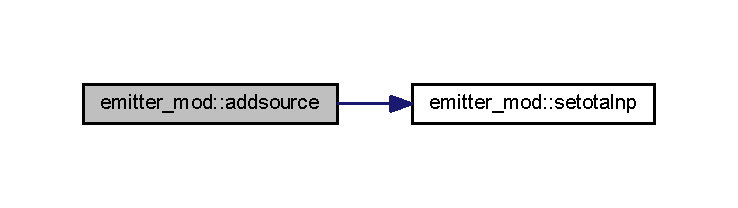
\includegraphics[width=350pt]{namespaceemitter__mod_ab704fb0e2eb9b3b4b9542706b6fb4eaf_cgraph}
\end{center}
\end{figure}
\mbox{\Hypertarget{namespaceemitter__mod_a7c677125988390e4c57909e4ea82d902}\label{namespaceemitter__mod_a7c677125988390e4c57909e4ea82d902}} 
\index{emitter\+\_\+mod@{emitter\+\_\+mod}!alloctracers@{alloctracers}}
\index{alloctracers@{alloctracers}!emitter\+\_\+mod@{emitter\+\_\+mod}}
\subsubsection{\texorpdfstring{alloctracers()}{alloctracers()}}
{\footnotesize\ttfamily subroutine emitter\+\_\+mod\+::alloctracers (\begin{DoxyParamCaption}\item[{class(\hyperlink{structemitter__mod_1_1emitter__class}{emitter\+\_\+class}), intent(inout)}]{self,  }\item[{class(\hyperlink{structsources__mod_1_1source__class}{source\+\_\+class}), intent(inout)}]{src }\end{DoxyParamCaption})\hspace{0.3cm}{\ttfamily [private]}}



method that allocates the tracers respective to a given source 

\begin{DoxyAuthor}{Author}
Ricardo Birjukovs Canelas -\/ M\+A\+R\+E\+T\+EC 
\end{DoxyAuthor}

\begin{DoxyParams}[1]{Parameters}
\mbox{\tt in}  & {\em self,src} & \\
\hline
\end{DoxyParams}
\mbox{\Hypertarget{namespaceemitter__mod_a6376ad0f8e1739b29caf672aa0750373}\label{namespaceemitter__mod_a6376ad0f8e1739b29caf672aa0750373}} 
\index{emitter\+\_\+mod@{emitter\+\_\+mod}!initializeemitter@{initializeemitter}}
\index{initializeemitter@{initializeemitter}!emitter\+\_\+mod@{emitter\+\_\+mod}}
\subsubsection{\texorpdfstring{initializeemitter()}{initializeemitter()}}
{\footnotesize\ttfamily subroutine emitter\+\_\+mod\+::initializeemitter (\begin{DoxyParamCaption}\item[{class(\hyperlink{structemitter__mod_1_1emitter__class}{emitter\+\_\+class}), intent(inout)}]{self }\end{DoxyParamCaption})\hspace{0.3cm}{\ttfamily [private]}}



method that initializes an emmiter class object. Sets default values 

\begin{DoxyAuthor}{Author}
Ricardo Birjukovs Canelas -\/ M\+A\+R\+E\+T\+EC 
\end{DoxyAuthor}

\begin{DoxyParams}[1]{Parameters}
\mbox{\tt in}  & {\em self} & \\
\hline
\end{DoxyParams}
\mbox{\Hypertarget{namespaceemitter__mod_ad89dfc083eae7362441c353225a74ebc}\label{namespaceemitter__mod_ad89dfc083eae7362441c353225a74ebc}} 
\index{emitter\+\_\+mod@{emitter\+\_\+mod}!initracers@{initracers}}
\index{initracers@{initracers}!emitter\+\_\+mod@{emitter\+\_\+mod}}
\subsubsection{\texorpdfstring{initracers()}{initracers()}}
{\footnotesize\ttfamily subroutine emitter\+\_\+mod\+::initracers (\begin{DoxyParamCaption}\item[{class(\hyperlink{structemitter__mod_1_1emitter__class}{emitter\+\_\+class}), intent(inout)}]{self,  }\item[{class(\hyperlink{structsources__mod_1_1source__class}{source\+\_\+class}), dimension(\+:), intent(inout)}]{srcs }\end{DoxyParamCaption})\hspace{0.3cm}{\ttfamily [private]}}



method that calls the tracer initialization from the emmiter object 

\begin{DoxyAuthor}{Author}
Ricardo Birjukovs Canelas -\/ M\+A\+R\+E\+T\+EC 
\end{DoxyAuthor}

\begin{DoxyParams}[1]{Parameters}
\mbox{\tt in}  & {\em self,src} & \\
\hline
\end{DoxyParams}
\mbox{\Hypertarget{namespaceemitter__mod_a5c219dd6692a761ad4bf968ae750fcc6}\label{namespaceemitter__mod_a5c219dd6692a761ad4bf968ae750fcc6}} 
\index{emitter\+\_\+mod@{emitter\+\_\+mod}!setotalnp@{setotalnp}}
\index{setotalnp@{setotalnp}!emitter\+\_\+mod@{emitter\+\_\+mod}}
\subsubsection{\texorpdfstring{setotalnp()}{setotalnp()}}
{\footnotesize\ttfamily subroutine emitter\+\_\+mod\+::setotalnp (\begin{DoxyParamCaption}\item[{class(\hyperlink{structsources__mod_1_1source__class}{source\+\_\+class}), intent(inout)}]{src }\end{DoxyParamCaption})\hspace{0.3cm}{\ttfamily [private]}}



private routine that returns the total number of tracers an input source will potentially create 

\begin{DoxyAuthor}{Author}
Ricardo Birjukovs Canelas -\/ M\+A\+R\+E\+T\+EC 
\end{DoxyAuthor}

\begin{DoxyParams}[1]{Parameters}
\mbox{\tt in}  & {\em src} & \\
\hline
\end{DoxyParams}
${NP}_{total}^{source-i}=(T_{end}^{source-i}-T_{start}^{source-i})*{Rate}^{source-i}*{NP}_{emission}^{source-i}$ Here is the caller graph for this function\+:\nopagebreak
\begin{figure}[H]
\begin{center}
\leavevmode
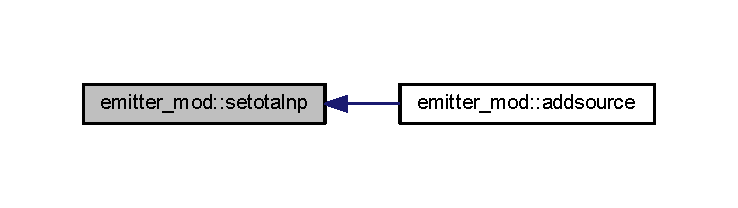
\includegraphics[width=350pt]{namespaceemitter__mod_a5c219dd6692a761ad4bf968ae750fcc6_icgraph}
\end{center}
\end{figure}

\hypertarget{namespacefieldtypes__mod}{}\section{fieldtypes\+\_\+mod Module Reference}
\label{namespacefieldtypes__mod}\index{fieldtypes\+\_\+mod@{fieldtypes\+\_\+mod}}


Defines classes for \textquotesingle{}fields\textquotesingle{}\+: 1, 2, 3 and 4D labeled data. Valid for both scalar and vectorial (real) data. Defines a generic wrapper for these classes, that abstracts the user from having to choose their data dimensionality or type to create a field.  


\subsection*{Data Types}
\begin{DoxyCompactItemize}
\item 
type \mbox{\hyperlink{structfieldtypes__mod_1_1field__class}{field\+\_\+class}}
\item 
type \mbox{\hyperlink{structfieldtypes__mod_1_1generic__field__class}{generic\+\_\+field\+\_\+class}}
\begin{DoxyCompactList}\small\item\em generic field class. This works as a wrapper for a generic initialization routine. \end{DoxyCompactList}\item 
type \mbox{\hyperlink{structfieldtypes__mod_1_1scalar1d__field__class}{scalar1d\+\_\+field\+\_\+class}}
\begin{DoxyCompactList}\small\item\em a 1D scalar field class \end{DoxyCompactList}\item 
type \mbox{\hyperlink{structfieldtypes__mod_1_1scalar2d__field__class}{scalar2d\+\_\+field\+\_\+class}}
\begin{DoxyCompactList}\small\item\em a 2D scalar field class \end{DoxyCompactList}\item 
type \mbox{\hyperlink{structfieldtypes__mod_1_1scalar3d__field__class}{scalar3d\+\_\+field\+\_\+class}}
\begin{DoxyCompactList}\small\item\em a 3D scalar field class \end{DoxyCompactList}\item 
type \mbox{\hyperlink{structfieldtypes__mod_1_1scalar4d__field__class}{scalar4d\+\_\+field\+\_\+class}}
\begin{DoxyCompactList}\small\item\em a 4D scalar field class \end{DoxyCompactList}\item 
type \mbox{\hyperlink{structfieldtypes__mod_1_1scalar__field__class}{scalar\+\_\+field\+\_\+class}}
\begin{DoxyCompactList}\small\item\em a scalar field class \end{DoxyCompactList}\item 
type \mbox{\hyperlink{structfieldtypes__mod_1_1vectorial2d__field__class}{vectorial2d\+\_\+field\+\_\+class}}
\begin{DoxyCompactList}\small\item\em a 2D vectorial field class \end{DoxyCompactList}\item 
type \mbox{\hyperlink{structfieldtypes__mod_1_1vectorial3d__field__class}{vectorial3d\+\_\+field\+\_\+class}}
\begin{DoxyCompactList}\small\item\em a 3D vectorial field class \end{DoxyCompactList}\item 
type \mbox{\hyperlink{structfieldtypes__mod_1_1vectorial4d__field__class}{vectorial4d\+\_\+field\+\_\+class}}
\begin{DoxyCompactList}\small\item\em a 4D vectorial field class \end{DoxyCompactList}\item 
type \mbox{\hyperlink{structfieldtypes__mod_1_1vectorial__field__class}{vectorial\+\_\+field\+\_\+class}}
\begin{DoxyCompactList}\small\item\em a vectorial field class \end{DoxyCompactList}\end{DoxyCompactItemize}
\subsection*{Functions/\+Subroutines}
\begin{DoxyCompactItemize}
\item 
subroutine \mbox{\hyperlink{namespacefieldtypes__mod_a67cc0dfdc7206a2769746ff7879a4375}{concatenate}} (self, gfield, used\+Posi)
\begin{DoxyCompactList}\small\item\em Method concatenates two fields by their last dimension. \end{DoxyCompactList}\item 
logical function \mbox{\hyperlink{namespacefieldtypes__mod_aad356f6f10d8edc58c56f02c796423f3}{compare}} (self, gfield)
\begin{DoxyCompactList}\small\item\em Method that compares the metadata of a scalar 1D field to the object field. \end{DoxyCompactList}\item 
subroutine \mbox{\hyperlink{namespacefieldtypes__mod_ad8f3bf57dafb3eac18e5a3198e36047c}{replacemetadata}} (self, name, units)
\begin{DoxyCompactList}\small\item\em replaces metadata on a generic field \end{DoxyCompactList}\item 
subroutine \mbox{\hyperlink{namespacefieldtypes__mod_a1d491079d69fb297c4fedd4f37d85e8e}{cleanfield}} (self)
\begin{DoxyCompactList}\small\item\em cleans a generic field \end{DoxyCompactList}\item 
subroutine \mbox{\hyperlink{namespacefieldtypes__mod_a4ec7b627804dfcdf20e3374ecc1cf459}{delgfield}} (self)
\item 
subroutine \mbox{\hyperlink{namespacefieldtypes__mod_a3f1571ad15733a3f2fff43e35f309416}{inits1d}} (self, name, units, field)
\begin{DoxyCompactList}\small\item\em Method that allocates and initializes a scalar 1D field in a generic field. \end{DoxyCompactList}\item 
integer function \mbox{\hyperlink{namespacefieldtypes__mod_afad53b4aed8733a243672c2dc19f62f3}{getfieldnearestindex}} (self, value)
\begin{DoxyCompactList}\small\item\em Method that returns the field\textquotesingle{}s nearest value index (scalar) \end{DoxyCompactList}\item 
subroutine \mbox{\hyperlink{namespacefieldtypes__mod_ad3329e97ec60bf9226d19be45ed21859}{inits2d}} (self, name, units, field)
\begin{DoxyCompactList}\small\item\em Method that allocates and initializes a scalar 2D field in a generic field. \end{DoxyCompactList}\item 
subroutine \mbox{\hyperlink{namespacefieldtypes__mod_a750ce2c729d98ea7031c839a3a5ebd7c}{inits3d}} (self, name, units, field)
\begin{DoxyCompactList}\small\item\em Method that allocates and initializes a scalar 3D field in a generic field. \end{DoxyCompactList}\item 
subroutine \mbox{\hyperlink{namespacefieldtypes__mod_a1987bd94293cfd9e35016ac5992501cd}{inits4d}} (self, name, units, field)
\begin{DoxyCompactList}\small\item\em Method that allocates and initializes a scalar 4D field in a generic field. \end{DoxyCompactList}\item 
subroutine \mbox{\hyperlink{namespacefieldtypes__mod_ad1af664e23793260f9c2fcd03829a1f5}{initv2d}} (self, name, units, field)
\begin{DoxyCompactList}\small\item\em Method that allocates and initializes a vectorial 2D field in a generic field. \end{DoxyCompactList}\item 
subroutine \mbox{\hyperlink{namespacefieldtypes__mod_aa0a152c9e5131d3003cc34e4f3b2974d}{initv3d}} (self, name, units, field)
\begin{DoxyCompactList}\small\item\em Method that allocates and initializes a vectorial 3D field in a generic field. \end{DoxyCompactList}\item 
subroutine \mbox{\hyperlink{namespacefieldtypes__mod_a08d665678bea0956a323d08863e164e5}{initv4d}} (self, name, units, field)
\begin{DoxyCompactList}\small\item\em Method that allocates and initializes a vectorial 4D field in a generic field. \end{DoxyCompactList}\item 
subroutine \mbox{\hyperlink{namespacefieldtypes__mod_a96ff5318da6a7db8bb61c525315c1c89}{initscalar1dfield}} (self, name, units, dim, field)
\begin{DoxyCompactList}\small\item\em Method that initializes a scalar 1D field. \end{DoxyCompactList}\item 
subroutine \mbox{\hyperlink{namespacefieldtypes__mod_aeb05bd1de9be296711016ad5b607a091}{cleanscalar1dfield}} (self)
\begin{DoxyCompactList}\small\item\em Method that initializes a scalar 1D field. \end{DoxyCompactList}\item 
subroutine \mbox{\hyperlink{namespacefieldtypes__mod_a1a3160727c99017639d758aad9031df5}{initscalar2dfield}} (self, name, units, dim, field)
\begin{DoxyCompactList}\small\item\em Method that initializes a scalar 2D field. \end{DoxyCompactList}\item 
subroutine \mbox{\hyperlink{namespacefieldtypes__mod_a26a4170db6067cf4ba85099f9701ff4c}{cleanscalar2dfield}} (self)
\begin{DoxyCompactList}\small\item\em Method that deallocates a scalar 2D field. \end{DoxyCompactList}\item 
subroutine \mbox{\hyperlink{namespacefieldtypes__mod_a3f2b90bc391ea5b84ead8069ee90f515}{initscalar3dfield}} (self, name, units, dim, field)
\begin{DoxyCompactList}\small\item\em Method that initializes a scalar 3D field. \end{DoxyCompactList}\item 
subroutine \mbox{\hyperlink{namespacefieldtypes__mod_a9f3716bcbd2524ed608c86920cab8693}{cleanscalar3dfield}} (self)
\begin{DoxyCompactList}\small\item\em Method that deallocates a scalar 3D field. \end{DoxyCompactList}\item 
subroutine \mbox{\hyperlink{namespacefieldtypes__mod_a21dba84bb8fdb02d8bf5fd0052b51283}{initscalar4dfield}} (self, name, units, dim, field)
\begin{DoxyCompactList}\small\item\em Method that initializes a scalar 4D field. \end{DoxyCompactList}\item 
subroutine \mbox{\hyperlink{namespacefieldtypes__mod_aaabae216913c347395d5e19ea2c22286}{cleanscalar4dfield}} (self)
\begin{DoxyCompactList}\small\item\em Method that deallocates a scalar 4D field. \end{DoxyCompactList}\item 
subroutine \mbox{\hyperlink{namespacefieldtypes__mod_ac3e3d9aabba3893d61583e890e3bdf41}{initvectorial2dfield}} (self, name, units, dim, field)
\begin{DoxyCompactList}\small\item\em Method that initializes a vectorial 2D field. \end{DoxyCompactList}\item 
subroutine \mbox{\hyperlink{namespacefieldtypes__mod_a20d935cfa1513350667d04f969be5e26}{initvectorial3dfield}} (self, name, units, dim, field)
\begin{DoxyCompactList}\small\item\em Method that initializes a vectorial 3D field. \end{DoxyCompactList}\item 
subroutine \mbox{\hyperlink{namespacefieldtypes__mod_ad458710e4a2d6c40a3dfa7f19481cd5a}{initvectorial4dfield}} (self, name, units, dim, field)
\begin{DoxyCompactList}\small\item\em Method that initializes a vectorial 4D field. \end{DoxyCompactList}\item 
subroutine \mbox{\hyperlink{namespacefieldtypes__mod_abc601ce9f8a974f426e876cc4c02e2a2}{setfieldmetadata}} (self, name, units, dim)
\begin{DoxyCompactList}\small\item\em Method that initializes a base field object by filling metadata. \end{DoxyCompactList}\item 
subroutine \mbox{\hyperlink{namespacefieldtypes__mod_a63d399d72fffde3fe8169b76cce59259}{printgenericfield}} (self)
\begin{DoxyCompactList}\small\item\em Method that prints the generic field information. \end{DoxyCompactList}\item 
type(string) function \mbox{\hyperlink{namespacefieldtypes__mod_abd34452f9afd91c4b9eeb60c51908312}{getgfieldtype}} (self)
\begin{DoxyCompactList}\small\item\em Method that returns the field type (scalar or vectorial), in a string, of a generic field. \end{DoxyCompactList}\item 
subroutine \mbox{\hyperlink{namespacefieldtypes__mod_a0babd6327ed77199d5437d17de34bafe}{test}} (self)
\begin{DoxyCompactList}\small\item\em A class \textquotesingle{}unit\textquotesingle{} test for the \mbox{\hyperlink{structfieldtypes__mod_1_1generic__field__class}{generic\+\_\+field\+\_\+class}}. \end{DoxyCompactList}\item 
subroutine \mbox{\hyperlink{namespacefieldtypes__mod_a5a556fba603c1d39b20713fdbc813332}{printfield}} (self)
\begin{DoxyCompactList}\small\item\em Method that prints the field information. \end{DoxyCompactList}\item 
type(string) function \mbox{\hyperlink{namespacefieldtypes__mod_a5faf9c157541acaa9681be2d59eda850}{getfieldtype}} (self)
\begin{DoxyCompactList}\small\item\em Method that returns the field type (scalar or vectorial), in a string. \end{DoxyCompactList}\item 
type(\mbox{\hyperlink{structfieldtypes__mod_1_1generic__field__class}{generic\+\_\+field\+\_\+class}}) function \mbox{\hyperlink{namespacefieldtypes__mod_ac35041b0ab166699a4fda1d0fa02ec67}{getfieldslice}} (self, llbound, uubound)
\begin{DoxyCompactList}\small\item\em Method that returns a slice of a field stored on a generic field. \end{DoxyCompactList}\item 
integer function, dimension(\+:), allocatable \mbox{\hyperlink{namespacefieldtypes__mod_ab8a0fa52771fc81b6f8a39cbb9ad2c34}{getfieldshape}} (self)
\begin{DoxyCompactList}\small\item\em Method that returns a slice of a field stored on a generic field. \end{DoxyCompactList}\item 
real(prec) function \mbox{\hyperlink{namespacefieldtypes__mod_a1012f73b2800753dd774d0dbff861b6f}{getfieldmaxbound}} (self)
\begin{DoxyCompactList}\small\item\em Method that returns the field\textquotesingle{}s maximum value (scalar) \end{DoxyCompactList}\item 
real(prec) function \mbox{\hyperlink{namespacefieldtypes__mod_aec092e7c0b82a7b3a828ae18af80b810}{getfieldminbound}} (self)
\begin{DoxyCompactList}\small\item\em Method that returns the field\textquotesingle{}s minimum value (scalar) \end{DoxyCompactList}\item 
subroutine \mbox{\hyperlink{namespacefieldtypes__mod_a214565d2002baff775a030611630fc32}{getgfield}} (self, a\+Field)
\begin{DoxyCompactList}\small\item\em method that initializes a generic field object given a field object \end{DoxyCompactList}\end{DoxyCompactItemize}


\subsection{Detailed Description}
Defines classes for \textquotesingle{}fields\textquotesingle{}\+: 1, 2, 3 and 4D labeled data. Valid for both scalar and vectorial (real) data. Defines a generic wrapper for these classes, that abstracts the user from having to choose their data dimensionality or type to create a field. 

\begin{DoxyAuthor}{Author}
Ricardo Birjukovs Canelas 
\end{DoxyAuthor}


\subsection{Function/\+Subroutine Documentation}
\mbox{\Hypertarget{namespacefieldtypes__mod_a1d491079d69fb297c4fedd4f37d85e8e}\label{namespacefieldtypes__mod_a1d491079d69fb297c4fedd4f37d85e8e}} 
\index{fieldtypes\+\_\+mod@{fieldtypes\+\_\+mod}!cleanfield@{cleanfield}}
\index{cleanfield@{cleanfield}!fieldtypes\+\_\+mod@{fieldtypes\+\_\+mod}}
\subsubsection{\texorpdfstring{cleanfield()}{cleanfield()}}
{\footnotesize\ttfamily subroutine fieldtypes\+\_\+mod\+::cleanfield (\begin{DoxyParamCaption}\item[{class(\mbox{\hyperlink{structfieldtypes__mod_1_1generic__field__class}{generic\+\_\+field\+\_\+class}}), intent(inout)}]{self }\end{DoxyParamCaption})\hspace{0.3cm}{\ttfamily [private]}}



cleans a generic field 

\begin{DoxyAuthor}{Author}
Ricardo Birjukovs Canelas -\/ M\+A\+R\+E\+T\+EC 
\end{DoxyAuthor}

\begin{DoxyParams}[1]{Parameters}
\mbox{\tt in}  & {\em self} & \\
\hline
\end{DoxyParams}


Definition at line 298 of file fields\+Types.\+f90.


\begin{DoxyCode}
298     \textcolor{keywordtype}{class}(generic\_field\_class), \textcolor{keywordtype}{intent(inout)} :: self
299     self%name = \textcolor{stringliteral}{''}
300     self%units = \textcolor{stringliteral}{''}
301     self%dim = mv
302     \textcolor{keywordflow}{if} (\textcolor{keyword}{allocated}(self%scalar1d%field)) \textcolor{keyword}{deallocate}(self%scalar1d%field)
303     \textcolor{keywordflow}{if} (\textcolor{keyword}{allocated}(self%scalar2d%field)) \textcolor{keyword}{deallocate}(self%scalar2d%field)
304     \textcolor{keywordflow}{if} (\textcolor{keyword}{allocated}(self%scalar3d%field)) \textcolor{keyword}{deallocate}(self%scalar3d%field)
305     \textcolor{keywordflow}{if} (\textcolor{keyword}{allocated}(self%scalar4d%field)) \textcolor{keyword}{deallocate}(self%scalar4d%field)
306     \textcolor{keywordflow}{if} (\textcolor{keyword}{allocated}(self%vectorial2d%field)) \textcolor{keyword}{deallocate}(self%vectorial2d%field)
307     \textcolor{keywordflow}{if} (\textcolor{keyword}{allocated}(self%vectorial3d%field)) \textcolor{keyword}{deallocate}(self%vectorial3d%field)
308     \textcolor{keywordflow}{if} (\textcolor{keyword}{allocated}(self%vectorial4d%field)) \textcolor{keyword}{deallocate}(self%vectorial4d%field)
\end{DoxyCode}
\mbox{\Hypertarget{namespacefieldtypes__mod_aeb05bd1de9be296711016ad5b607a091}\label{namespacefieldtypes__mod_aeb05bd1de9be296711016ad5b607a091}} 
\index{fieldtypes\+\_\+mod@{fieldtypes\+\_\+mod}!cleanscalar1dfield@{cleanscalar1dfield}}
\index{cleanscalar1dfield@{cleanscalar1dfield}!fieldtypes\+\_\+mod@{fieldtypes\+\_\+mod}}
\subsubsection{\texorpdfstring{cleanscalar1dfield()}{cleanscalar1dfield()}}
{\footnotesize\ttfamily subroutine fieldtypes\+\_\+mod\+::cleanscalar1dfield (\begin{DoxyParamCaption}\item[{class(\mbox{\hyperlink{structfieldtypes__mod_1_1scalar1d__field__class}{scalar1d\+\_\+field\+\_\+class}}), intent(out)}]{self }\end{DoxyParamCaption})\hspace{0.3cm}{\ttfamily [private]}}



Method that initializes a scalar 1D field. 

\begin{DoxyAuthor}{Author}
Ricardo Birjukovs Canelas -\/ M\+A\+R\+E\+T\+EC 
\end{DoxyAuthor}

\begin{DoxyParams}[1]{Parameters}
\mbox{\tt in}  & {\em self} & \\
\hline
\end{DoxyParams}


Definition at line 517 of file fields\+Types.\+f90.


\begin{DoxyCode}
517     \textcolor{keywordtype}{class}(scalar1d\_field\_class), \textcolor{keywordtype}{intent(out)} :: self
518     \textcolor{keywordflow}{if} (\textcolor{keyword}{allocated}(self%field)) \textcolor{keyword}{deallocate}(self%field)
\end{DoxyCode}
\mbox{\Hypertarget{namespacefieldtypes__mod_a26a4170db6067cf4ba85099f9701ff4c}\label{namespacefieldtypes__mod_a26a4170db6067cf4ba85099f9701ff4c}} 
\index{fieldtypes\+\_\+mod@{fieldtypes\+\_\+mod}!cleanscalar2dfield@{cleanscalar2dfield}}
\index{cleanscalar2dfield@{cleanscalar2dfield}!fieldtypes\+\_\+mod@{fieldtypes\+\_\+mod}}
\subsubsection{\texorpdfstring{cleanscalar2dfield()}{cleanscalar2dfield()}}
{\footnotesize\ttfamily subroutine fieldtypes\+\_\+mod\+::cleanscalar2dfield (\begin{DoxyParamCaption}\item[{class(\mbox{\hyperlink{structfieldtypes__mod_1_1scalar2d__field__class}{scalar2d\+\_\+field\+\_\+class}}), intent(out)}]{self }\end{DoxyParamCaption})\hspace{0.3cm}{\ttfamily [private]}}



Method that deallocates a scalar 2D field. 

\begin{DoxyAuthor}{Author}
Ricardo Birjukovs Canelas -\/ M\+A\+R\+E\+T\+EC 
\end{DoxyAuthor}

\begin{DoxyParams}[1]{Parameters}
\mbox{\tt in}  & {\em self} & \\
\hline
\end{DoxyParams}


Definition at line 544 of file fields\+Types.\+f90.


\begin{DoxyCode}
544     \textcolor{keywordtype}{class}(scalar2d\_field\_class), \textcolor{keywordtype}{intent(out)} :: self
545     \textcolor{keywordflow}{if} (\textcolor{keyword}{allocated}(self%field)) \textcolor{keyword}{deallocate}(self%field)
\end{DoxyCode}
\mbox{\Hypertarget{namespacefieldtypes__mod_a9f3716bcbd2524ed608c86920cab8693}\label{namespacefieldtypes__mod_a9f3716bcbd2524ed608c86920cab8693}} 
\index{fieldtypes\+\_\+mod@{fieldtypes\+\_\+mod}!cleanscalar3dfield@{cleanscalar3dfield}}
\index{cleanscalar3dfield@{cleanscalar3dfield}!fieldtypes\+\_\+mod@{fieldtypes\+\_\+mod}}
\subsubsection{\texorpdfstring{cleanscalar3dfield()}{cleanscalar3dfield()}}
{\footnotesize\ttfamily subroutine fieldtypes\+\_\+mod\+::cleanscalar3dfield (\begin{DoxyParamCaption}\item[{class(\mbox{\hyperlink{structfieldtypes__mod_1_1scalar3d__field__class}{scalar3d\+\_\+field\+\_\+class}}), intent(out)}]{self }\end{DoxyParamCaption})\hspace{0.3cm}{\ttfamily [private]}}



Method that deallocates a scalar 3D field. 

\begin{DoxyAuthor}{Author}
Ricardo Birjukovs Canelas -\/ M\+A\+R\+E\+T\+EC 
\end{DoxyAuthor}

\begin{DoxyParams}[1]{Parameters}
\mbox{\tt in}  & {\em self} & \\
\hline
\end{DoxyParams}


Definition at line 571 of file fields\+Types.\+f90.


\begin{DoxyCode}
571     \textcolor{keywordtype}{class}(scalar3d\_field\_class), \textcolor{keywordtype}{intent(out)} :: self
572     \textcolor{keywordflow}{if} (\textcolor{keyword}{allocated}(self%field)) \textcolor{keyword}{deallocate}(self%field)
\end{DoxyCode}
\mbox{\Hypertarget{namespacefieldtypes__mod_aaabae216913c347395d5e19ea2c22286}\label{namespacefieldtypes__mod_aaabae216913c347395d5e19ea2c22286}} 
\index{fieldtypes\+\_\+mod@{fieldtypes\+\_\+mod}!cleanscalar4dfield@{cleanscalar4dfield}}
\index{cleanscalar4dfield@{cleanscalar4dfield}!fieldtypes\+\_\+mod@{fieldtypes\+\_\+mod}}
\subsubsection{\texorpdfstring{cleanscalar4dfield()}{cleanscalar4dfield()}}
{\footnotesize\ttfamily subroutine fieldtypes\+\_\+mod\+::cleanscalar4dfield (\begin{DoxyParamCaption}\item[{class(\mbox{\hyperlink{structfieldtypes__mod_1_1scalar4d__field__class}{scalar4d\+\_\+field\+\_\+class}}), intent(out)}]{self }\end{DoxyParamCaption})\hspace{0.3cm}{\ttfamily [private]}}



Method that deallocates a scalar 4D field. 

\begin{DoxyAuthor}{Author}
Ricardo Birjukovs Canelas -\/ M\+A\+R\+E\+T\+EC 
\end{DoxyAuthor}

\begin{DoxyParams}[1]{Parameters}
\mbox{\tt in}  & {\em self} & \\
\hline
\end{DoxyParams}


Definition at line 598 of file fields\+Types.\+f90.


\begin{DoxyCode}
598     \textcolor{keywordtype}{class}(scalar4d\_field\_class), \textcolor{keywordtype}{intent(out)} :: self
599     \textcolor{keywordflow}{if} (\textcolor{keyword}{allocated}(self%field)) \textcolor{keyword}{deallocate}(self%field)
\end{DoxyCode}
\mbox{\Hypertarget{namespacefieldtypes__mod_aad356f6f10d8edc58c56f02c796423f3}\label{namespacefieldtypes__mod_aad356f6f10d8edc58c56f02c796423f3}} 
\index{fieldtypes\+\_\+mod@{fieldtypes\+\_\+mod}!compare@{compare}}
\index{compare@{compare}!fieldtypes\+\_\+mod@{fieldtypes\+\_\+mod}}
\subsubsection{\texorpdfstring{compare()}{compare()}}
{\footnotesize\ttfamily logical function fieldtypes\+\_\+mod\+::compare (\begin{DoxyParamCaption}\item[{class(\mbox{\hyperlink{structfieldtypes__mod_1_1generic__field__class}{generic\+\_\+field\+\_\+class}}), intent(inout)}]{self,  }\item[{class(\mbox{\hyperlink{structfieldtypes__mod_1_1generic__field__class}{generic\+\_\+field\+\_\+class}}), intent(in)}]{gfield }\end{DoxyParamCaption})\hspace{0.3cm}{\ttfamily [private]}}



Method that compares the metadata of a scalar 1D field to the object field. 

\begin{DoxyAuthor}{Author}
Ricardo Birjukovs Canelas -\/ M\+A\+R\+E\+T\+EC 
\end{DoxyAuthor}

\begin{DoxyParams}[1]{Parameters}
\mbox{\tt in}  & {\em self,gfield} & \\
\hline
\end{DoxyParams}


Definition at line 261 of file fields\+Types.\+f90.


\begin{DoxyCode}
261     \textcolor{keywordtype}{class}(generic\_field\_class), \textcolor{keywordtype}{intent(inout)} :: self
262     \textcolor{keywordtype}{class}(generic\_field\_class), \textcolor{keywordtype}{intent(in)} :: gfield
263     \textcolor{keywordtype}{type}(string) :: outext
264     comp = .true.
265     \textcolor{keywordflow}{if} (self%name /= gfield%name) comp = .false.
266     \textcolor{keywordflow}{if} (self%units /= gfield%units) comp = .false. \textcolor{comment}{!might be asking too much...}
267     \textcolor{keywordflow}{if} (self%dim /= gfield%dim) comp = .false.
268     \textcolor{keywordflow}{if} (\textcolor{keyword}{allocated}(self%scalar1d%field) .and. .not. \textcolor{keyword}{allocated}(gfield%scalar1d%field)) comp = .false.
269     \textcolor{keywordflow}{if} (\textcolor{keyword}{allocated}(self%scalar2d%field) .and. .not. \textcolor{keyword}{allocated}(gfield%scalar2d%field)) comp = .false.
270     \textcolor{keywordflow}{if} (\textcolor{keyword}{allocated}(self%scalar3d%field) .and. .not. \textcolor{keyword}{allocated}(gfield%scalar3d%field)) comp = .false.
271     \textcolor{keywordflow}{if} (\textcolor{keyword}{allocated}(self%scalar4d%field) .and. .not. \textcolor{keyword}{allocated}(gfield%scalar4d%field)) comp = .false.
272     \textcolor{keywordflow}{if} (\textcolor{keyword}{allocated}(self%vectorial2d%field) .and. .not. \textcolor{keyword}{allocated}(gfield%vectorial2d%field)) comp = .false.
273     \textcolor{keywordflow}{if} (\textcolor{keyword}{allocated}(self%vectorial3d%field) .and. .not. \textcolor{keyword}{allocated}(gfield%vectorial3d%field)) comp = .false.
274     \textcolor{keywordflow}{if} (\textcolor{keyword}{allocated}(self%vectorial4d%field) .and. .not. \textcolor{keyword}{allocated}(gfield%vectorial4d%field)) comp = .false.
\end{DoxyCode}
\mbox{\Hypertarget{namespacefieldtypes__mod_a67cc0dfdc7206a2769746ff7879a4375}\label{namespacefieldtypes__mod_a67cc0dfdc7206a2769746ff7879a4375}} 
\index{fieldtypes\+\_\+mod@{fieldtypes\+\_\+mod}!concatenate@{concatenate}}
\index{concatenate@{concatenate}!fieldtypes\+\_\+mod@{fieldtypes\+\_\+mod}}
\subsubsection{\texorpdfstring{concatenate()}{concatenate()}}
{\footnotesize\ttfamily subroutine fieldtypes\+\_\+mod\+::concatenate (\begin{DoxyParamCaption}\item[{class(\mbox{\hyperlink{structfieldtypes__mod_1_1generic__field__class}{generic\+\_\+field\+\_\+class}}), intent(inout)}]{self,  }\item[{type(\mbox{\hyperlink{structfieldtypes__mod_1_1generic__field__class}{generic\+\_\+field\+\_\+class}}), intent(in)}]{gfield,  }\item[{logical, dimension(\+:), intent(in), optional}]{used\+Posi }\end{DoxyParamCaption})\hspace{0.3cm}{\ttfamily [private]}}



Method concatenates two fields by their last dimension. 

\begin{DoxyAuthor}{Author}
Ricardo Birjukovs Canelas -\/ M\+A\+R\+E\+T\+EC 
\end{DoxyAuthor}

\begin{DoxyParams}[1]{Parameters}
\mbox{\tt in}  & {\em self,gfield,used\+Posi} & \\
\hline
\end{DoxyParams}


Definition at line 150 of file fields\+Types.\+f90.


\begin{DoxyCode}
150     \textcolor{keywordtype}{class}(generic\_field\_class), \textcolor{keywordtype}{intent(inout)} :: self
151     \textcolor{keywordtype}{type}(generic\_field\_class), \textcolor{keywordtype}{intent(in)} :: gfield
152     \textcolor{keywordtype}{logical}, \textcolor{keywordtype}{dimension(:)}, \textcolor{keywordtype}{optional}, \textcolor{keywordtype}{intent(in)} :: usedPosi 
153     \textcolor{keywordtype}{logical}, \textcolor{keywordtype}{allocatable}, \textcolor{keywordtype}{dimension(:)} :: usedPos
154     \textcolor{keywordtype}{integer} :: fDim, nUsedPos, i, j
155     \textcolor{keywordtype}{type}(string) :: fType
156     \textcolor{keywordtype}{real(prec)}, \textcolor{keywordtype}{allocatable}, \textcolor{keywordtype}{dimension(:)} :: field1d
157     \textcolor{keywordtype}{real(prec)}, \textcolor{keywordtype}{allocatable}, \textcolor{keywordtype}{dimension(:,:)} :: field2d
158     \textcolor{keywordtype}{real(prec)}, \textcolor{keywordtype}{allocatable}, \textcolor{keywordtype}{dimension(:,:,:)} :: field3d
159     \textcolor{keywordtype}{real(prec)}, \textcolor{keywordtype}{allocatable}, \textcolor{keywordtype}{dimension(:,:,:,:)} :: field4d
160 
161     fdim = self%dim
162     ftype = self%getGFieldType()
163     \textcolor{keywordflow}{if} (gfield%dim /= fdim) \textcolor{keywordflow}{return}
164     \textcolor{keywordflow}{if} (gfield%getGFieldType() /= ftype) \textcolor{keywordflow}{return}
165     
166     \textcolor{keywordflow}{if} (\textcolor{keyword}{present}(usedposi)) \textcolor{keywordflow}{then}
167         \textcolor{keyword}{allocate}(usedpos, source = usedposi)
168         nusedpos = count(usedpos)
169 \textcolor{keywordflow}{    end if}
170     
171     \textcolor{keywordflow}{if} (ftype == \textcolor{stringliteral}{'Scalar'}) \textcolor{keywordflow}{then}
172         \textcolor{keywordflow}{if} (fdim == 1) \textcolor{keywordflow}{then}
173             \textcolor{keywordflow}{if} (.not.\textcolor{keyword}{allocated}(usedpos)) \textcolor{keywordflow}{then}
174                 nusedpos = \textcolor{keyword}{size}(gfield%scalar1d%field)
175                 \textcolor{keyword}{allocate}(usedpos(nusedpos))
176                 usedpos = .true.
177 \textcolor{keywordflow}{            end if}
178             \textcolor{keyword}{allocate}(field1d(\textcolor{keyword}{size}(self%scalar1d%field) + nusedpos))
179             field1d(1:\textcolor{keyword}{size}(self%scalar1d%field)) = self%scalar1d%field
180             i= \textcolor{keyword}{size}(self%scalar1d%field)+1
181             \textcolor{keywordflow}{do} j= 1, \textcolor{keyword}{size}(usedpos)
182                 \textcolor{keywordflow}{if} (usedpos(j)) \textcolor{keywordflow}{then}
183                     field1d(i) = gfield%scalar1d%field(j)
184                     i= i+1
185 \textcolor{keywordflow}{                end if}
186 \textcolor{keywordflow}{            end do}
187             \textcolor{keyword}{deallocate}(self%scalar1d%field)
188             \textcolor{keyword}{allocate}(self%scalar1d%field(\textcolor{keyword}{size}(field1d)))
189             self%scalar1d%field = field1d
190 \textcolor{keywordflow}{        end if}
191         \textcolor{keywordflow}{if} (fdim == 2) \textcolor{keywordflow}{then}
192             \textcolor{keywordflow}{if} (.not.\textcolor{keyword}{allocated}(usedpos)) \textcolor{keywordflow}{then}
193                 nusedpos = \textcolor{keyword}{size}(gfield%scalar2d%field,2)
194                 \textcolor{keyword}{allocate}(usedpos(nusedpos))
195                 usedpos = .true.
196 \textcolor{keywordflow}{            end if}
197             \textcolor{keyword}{allocate}(field2d(\textcolor{keyword}{size}(self%scalar2d%field,1),\textcolor{keyword}{size}(self%scalar2d%field,2) + nusedpos))
198             field2d(:,1:\textcolor{keyword}{size}(self%scalar2d%field,2)) = self%scalar2d%field
199             i= \textcolor{keyword}{size}(self%scalar2d%field, 2) +1
200             \textcolor{keywordflow}{do} j= 1, \textcolor{keyword}{size}(usedpos)
201                 \textcolor{keywordflow}{if} (usedpos(j)) \textcolor{keywordflow}{then}
202                     field2d(:, i) = gfield%scalar2d%field(:, j)
203                     i= i+1
204 \textcolor{keywordflow}{                end if}
205 \textcolor{keywordflow}{            end do}            
206             \textcolor{keyword}{deallocate}(self%scalar2d%field)            
207             \textcolor{keyword}{allocate}(self%scalar2d%field(\textcolor{keyword}{size}(field2d,1), \textcolor{keyword}{size}(field2d,2)))
208             self%scalar2d%field = field2d
209 \textcolor{keywordflow}{        end if}
210         \textcolor{keywordflow}{if} (fdim == 3) \textcolor{keywordflow}{then}
211             \textcolor{keywordflow}{if} (.not.\textcolor{keyword}{allocated}(usedpos)) \textcolor{keywordflow}{then}
212                 nusedpos = \textcolor{keyword}{size}(gfield%scalar3d%field,3)
213                 \textcolor{keyword}{allocate}(usedpos(nusedpos))
214                 usedpos = .true.
215 \textcolor{keywordflow}{            end if}
216             \textcolor{keyword}{allocate}(field3d(\textcolor{keyword}{size}(self%scalar3d%field,1),\textcolor{keyword}{size}(self%scalar3d%field,2),\textcolor{keyword}{size}(self%scalar3d
      %field,3) + nusedpos))
217             field3d(:,:,1:\textcolor{keyword}{size}(self%scalar3d%field,3)) = self%scalar3d%field
218             i= \textcolor{keyword}{size}(self%scalar3d%field, 3) +1
219             \textcolor{keywordflow}{do} j= 1, \textcolor{keyword}{size}(usedpos)
220                 \textcolor{keywordflow}{if} (usedpos(j)) \textcolor{keywordflow}{then}
221                     field3d(:,:, i) = gfield%scalar3d%field(:,:, j)
222                     i= i+1
223 \textcolor{keywordflow}{                end if}
224 \textcolor{keywordflow}{            end do}
225             \textcolor{keyword}{deallocate}(self%scalar3d%field)
226             \textcolor{keyword}{allocate}(self%scalar3d%field(\textcolor{keyword}{size}(field3d,1), \textcolor{keyword}{size}(field3d,2), \textcolor{keyword}{size}(field3d,3)))
227             self%scalar3d%field = field3d
228 \textcolor{keywordflow}{        end if}
229         \textcolor{keywordflow}{if} (fdim == 4) \textcolor{keywordflow}{then}
230             \textcolor{keywordflow}{if} (.not.\textcolor{keyword}{allocated}(usedpos)) \textcolor{keywordflow}{then}
231                 nusedpos = \textcolor{keyword}{size}(gfield%scalar4d%field,4)
232                 \textcolor{keyword}{allocate}(usedpos(nusedpos))
233                 usedpos = .true.
234 \textcolor{keywordflow}{            end if}
235             \textcolor{keyword}{allocate}(field4d(\textcolor{keyword}{size}(self%scalar4d%field,1),\textcolor{keyword}{size}(self%scalar4d%field,2),\textcolor{keyword}{size}(self%scalar4d
      %field,3),\textcolor{keyword}{size}(self%scalar4d%field,4) + nusedpos))
236             field4d(:,:,:,1:\textcolor{keyword}{size}(self%scalar4d%field,4)) = self%scalar4d%field
237              i= \textcolor{keyword}{size}(self%scalar4d%field, 4) +1
238             \textcolor{keywordflow}{do} j= 1, \textcolor{keyword}{size}(usedpos)
239                 \textcolor{keywordflow}{if} (usedpos(j)) \textcolor{keywordflow}{then}
240                     field4d(:,:,:, i) = gfield%scalar4d%field(:,:,:, j)
241                     i= i+1
242 \textcolor{keywordflow}{                end if}
243 \textcolor{keywordflow}{            end do}
244             \textcolor{keyword}{deallocate}(self%scalar4d%field)
245             \textcolor{keyword}{allocate}(self%scalar4d%field(\textcolor{keyword}{size}(field4d,1), \textcolor{keyword}{size}(field4d,2), \textcolor{keyword}{size}(field4d,3), \textcolor{keyword}{size}(field4d,4)
      ))
246             self%scalar4d%field = field4d
247 \textcolor{keywordflow}{        end if}
248     \textcolor{keywordflow}{else} \textcolor{keywordflow}{if} (ftype == \textcolor{stringliteral}{'Vectorial'}) \textcolor{keywordflow}{then}
249         \textcolor{keywordflow}{return}
250 \textcolor{keywordflow}{    end if}
251 
\end{DoxyCode}
\mbox{\Hypertarget{namespacefieldtypes__mod_a4ec7b627804dfcdf20e3374ecc1cf459}\label{namespacefieldtypes__mod_a4ec7b627804dfcdf20e3374ecc1cf459}} 
\index{fieldtypes\+\_\+mod@{fieldtypes\+\_\+mod}!delgfield@{delgfield}}
\index{delgfield@{delgfield}!fieldtypes\+\_\+mod@{fieldtypes\+\_\+mod}}
\subsubsection{\texorpdfstring{delgfield()}{delgfield()}}
{\footnotesize\ttfamily subroutine fieldtypes\+\_\+mod\+::delgfield (\begin{DoxyParamCaption}\item[{type(\mbox{\hyperlink{structfieldtypes__mod_1_1generic__field__class}{generic\+\_\+field\+\_\+class}}), intent(inout)}]{self }\end{DoxyParamCaption})\hspace{0.3cm}{\ttfamily [private]}}



Definition at line 312 of file fields\+Types.\+f90.


\begin{DoxyCode}
312     \textcolor{keywordtype}{type}(generic\_field\_class), \textcolor{keywordtype}{intent(inout)} :: self
313     self%name = \textcolor{stringliteral}{''}
314     self%units = \textcolor{stringliteral}{''}
315     self%dim = mv
316     \textcolor{keywordflow}{if} (\textcolor{keyword}{allocated}(self%scalar1d%field)) \textcolor{keyword}{deallocate}(self%scalar1d%field)
317     \textcolor{keywordflow}{if} (\textcolor{keyword}{allocated}(self%scalar2d%field)) \textcolor{keyword}{deallocate}(self%scalar2d%field)
318     \textcolor{keywordflow}{if} (\textcolor{keyword}{allocated}(self%scalar3d%field)) \textcolor{keyword}{deallocate}(self%scalar3d%field)
319     \textcolor{keywordflow}{if} (\textcolor{keyword}{allocated}(self%scalar4d%field)) \textcolor{keyword}{deallocate}(self%scalar4d%field)
320     \textcolor{keywordflow}{if} (\textcolor{keyword}{allocated}(self%vectorial2d%field)) \textcolor{keyword}{deallocate}(self%vectorial2d%field)
321     \textcolor{keywordflow}{if} (\textcolor{keyword}{allocated}(self%vectorial3d%field)) \textcolor{keyword}{deallocate}(self%vectorial3d%field)
322     \textcolor{keywordflow}{if} (\textcolor{keyword}{allocated}(self%vectorial4d%field)) \textcolor{keyword}{deallocate}(self%vectorial4d%field)
\end{DoxyCode}
Here is the caller graph for this function\+:\nopagebreak
\begin{figure}[H]
\begin{center}
\leavevmode
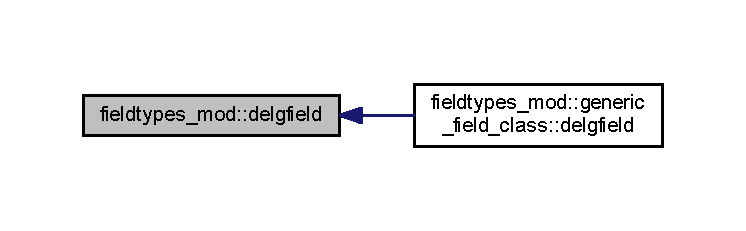
\includegraphics[width=350pt]{namespacefieldtypes__mod_a4ec7b627804dfcdf20e3374ecc1cf459_icgraph}
\end{center}
\end{figure}
\mbox{\Hypertarget{namespacefieldtypes__mod_a1012f73b2800753dd774d0dbff861b6f}\label{namespacefieldtypes__mod_a1012f73b2800753dd774d0dbff861b6f}} 
\index{fieldtypes\+\_\+mod@{fieldtypes\+\_\+mod}!getfieldmaxbound@{getfieldmaxbound}}
\index{getfieldmaxbound@{getfieldmaxbound}!fieldtypes\+\_\+mod@{fieldtypes\+\_\+mod}}
\subsubsection{\texorpdfstring{getfieldmaxbound()}{getfieldmaxbound()}}
{\footnotesize\ttfamily real(prec) function fieldtypes\+\_\+mod\+::getfieldmaxbound (\begin{DoxyParamCaption}\item[{class(\mbox{\hyperlink{structfieldtypes__mod_1_1field__class}{field\+\_\+class}}), intent(in)}]{self }\end{DoxyParamCaption})\hspace{0.3cm}{\ttfamily [private]}}



Method that returns the field\textquotesingle{}s maximum value (scalar) 

\begin{DoxyAuthor}{Author}
Ricardo Birjukovs Canelas -\/ M\+A\+R\+E\+T\+EC 
\end{DoxyAuthor}


Definition at line 857 of file fields\+Types.\+f90.


\begin{DoxyCode}
857     \textcolor{keywordtype}{class}(field\_class), \textcolor{keywordtype}{intent(in)} :: self
858     \textcolor{keywordtype}{type}(string) :: outext
859     \textcolor{keywordflow}{select type}(self)
860 \textcolor{keywordflow}{    class is} (scalar\_field\_class)
861 \textcolor{keywordflow}{    class is} (scalar1d\_field\_class)
862         getfieldmaxbound = maxval(self%field)
863 \textcolor{keywordflow}{    class is} (scalar2d\_field\_class)
864         getfieldmaxbound = maxval(self%field)
865 \textcolor{keywordflow}{    class is} (scalar3d\_field\_class)
866         getfieldmaxbound = maxval(self%field)
867 \textcolor{keywordflow}{    class is} (scalar4d\_field\_class)
868         getfieldmaxbound = maxval(self%field)
869 \textcolor{keywordflow}{    class is} (vectorial\_field\_class)
870         getfieldmaxbound = mv
871 \textcolor{keywordflow}{        class default}
872         outext = \textcolor{stringliteral}{'[field\_class::getFieldMaxBound]: Unexepected type of content, not a scalar or vectorial
       Field'}
873         \textcolor{keyword}{call }log%put(outext)
874         stop
875 \textcolor{keywordflow}{    end select}
\end{DoxyCode}
\mbox{\Hypertarget{namespacefieldtypes__mod_aec092e7c0b82a7b3a828ae18af80b810}\label{namespacefieldtypes__mod_aec092e7c0b82a7b3a828ae18af80b810}} 
\index{fieldtypes\+\_\+mod@{fieldtypes\+\_\+mod}!getfieldminbound@{getfieldminbound}}
\index{getfieldminbound@{getfieldminbound}!fieldtypes\+\_\+mod@{fieldtypes\+\_\+mod}}
\subsubsection{\texorpdfstring{getfieldminbound()}{getfieldminbound()}}
{\footnotesize\ttfamily real(prec) function fieldtypes\+\_\+mod\+::getfieldminbound (\begin{DoxyParamCaption}\item[{class(\mbox{\hyperlink{structfieldtypes__mod_1_1field__class}{field\+\_\+class}}), intent(in)}]{self }\end{DoxyParamCaption})\hspace{0.3cm}{\ttfamily [private]}}



Method that returns the field\textquotesingle{}s minimum value (scalar) 

\begin{DoxyAuthor}{Author}
Ricardo Birjukovs Canelas -\/ M\+A\+R\+E\+T\+EC 
\end{DoxyAuthor}


Definition at line 884 of file fields\+Types.\+f90.


\begin{DoxyCode}
884     \textcolor{keywordtype}{class}(field\_class), \textcolor{keywordtype}{intent(in)} :: self
885     \textcolor{keywordtype}{type}(string) :: outext
886     \textcolor{keywordflow}{select type}(self)
887 \textcolor{keywordflow}{    class is} (scalar\_field\_class)
888 \textcolor{keywordflow}{    class is} (scalar1d\_field\_class)
889         getfieldminbound = minval(self%field)
890 \textcolor{keywordflow}{    class is} (scalar2d\_field\_class)
891         getfieldminbound = minval(self%field)
892 \textcolor{keywordflow}{    class is} (scalar3d\_field\_class)
893         getfieldminbound = minval(self%field)
894 \textcolor{keywordflow}{    class is} (scalar4d\_field\_class)
895         getfieldminbound = minval(self%field)
896 \textcolor{keywordflow}{    class is} (vectorial\_field\_class)
897         getfieldminbound = mv
898 \textcolor{keywordflow}{        class default}
899         outext = \textcolor{stringliteral}{'[field\_class::getFieldMinBound]: Unexepected type of content, not a scalar or vectorial
       Field'}
900         \textcolor{keyword}{call }log%put(outext)
901         stop
902 \textcolor{keywordflow}{    end select}
\end{DoxyCode}
\mbox{\Hypertarget{namespacefieldtypes__mod_afad53b4aed8733a243672c2dc19f62f3}\label{namespacefieldtypes__mod_afad53b4aed8733a243672c2dc19f62f3}} 
\index{fieldtypes\+\_\+mod@{fieldtypes\+\_\+mod}!getfieldnearestindex@{getfieldnearestindex}}
\index{getfieldnearestindex@{getfieldnearestindex}!fieldtypes\+\_\+mod@{fieldtypes\+\_\+mod}}
\subsubsection{\texorpdfstring{getfieldnearestindex()}{getfieldnearestindex()}}
{\footnotesize\ttfamily integer function fieldtypes\+\_\+mod\+::getfieldnearestindex (\begin{DoxyParamCaption}\item[{class(\mbox{\hyperlink{structfieldtypes__mod_1_1scalar1d__field__class}{scalar1d\+\_\+field\+\_\+class}}), intent(in)}]{self,  }\item[{real(prec), intent(in)}]{value }\end{DoxyParamCaption})\hspace{0.3cm}{\ttfamily [private]}}



Method that returns the field\textquotesingle{}s nearest value index (scalar) 

\begin{DoxyAuthor}{Author}
Ricardo Birjukovs Canelas -\/ M\+A\+R\+E\+T\+EC 
\end{DoxyAuthor}

\begin{DoxyParams}[1]{Parameters}
\mbox{\tt in}  & {\em self,value} & \\
\hline
\end{DoxyParams}


Definition at line 354 of file fields\+Types.\+f90.


\begin{DoxyCode}
354     \textcolor{keywordtype}{class}(scalar1d\_field\_class), \textcolor{keywordtype}{intent(in)} :: self
355     \textcolor{keywordtype}{real(prec)}, \textcolor{keywordtype}{intent(in)} :: value
356     \textcolor{keywordtype}{real(prec)}, \textcolor{keywordtype}{allocatable}, \textcolor{keywordtype}{dimension(:)} :: comp
357     \textcolor{keyword}{allocate}(comp(\textcolor{keyword}{size}(self%field)))
358     comp = \textcolor{keywordtype}{value}
359     getfieldnearestindex = minloc(abs(comp - self%field), dim=1)
\end{DoxyCode}
\mbox{\Hypertarget{namespacefieldtypes__mod_ab8a0fa52771fc81b6f8a39cbb9ad2c34}\label{namespacefieldtypes__mod_ab8a0fa52771fc81b6f8a39cbb9ad2c34}} 
\index{fieldtypes\+\_\+mod@{fieldtypes\+\_\+mod}!getfieldshape@{getfieldshape}}
\index{getfieldshape@{getfieldshape}!fieldtypes\+\_\+mod@{fieldtypes\+\_\+mod}}
\subsubsection{\texorpdfstring{getfieldshape()}{getfieldshape()}}
{\footnotesize\ttfamily integer function, dimension(\+:), allocatable fieldtypes\+\_\+mod\+::getfieldshape (\begin{DoxyParamCaption}\item[{class(\mbox{\hyperlink{structfieldtypes__mod_1_1field__class}{field\+\_\+class}}), intent(in)}]{self }\end{DoxyParamCaption})\hspace{0.3cm}{\ttfamily [private]}}



Method that returns a slice of a field stored on a generic field. 

\begin{DoxyAuthor}{Author}
Ricardo Birjukovs Canelas -\/ M\+A\+R\+E\+T\+EC 
\end{DoxyAuthor}


Definition at line 820 of file fields\+Types.\+f90.


\begin{DoxyCode}
820     \textcolor{keywordtype}{class}(field\_class), \textcolor{keywordtype}{intent(in)} :: self
821     \textcolor{keywordtype}{integer}, \textcolor{keywordtype}{allocatable}, \textcolor{keywordtype}{dimension(:)} :: getFieldShape
822     \textcolor{keywordtype}{type}(string) :: outext
823 
824     \textcolor{keywordflow}{select type}(self)
825 \textcolor{keywordflow}{    class is} (scalar\_field\_class)
826 \textcolor{keywordflow}{    class is} (scalar1d\_field\_class)
827         \textcolor{keyword}{allocate}(getfieldshape(1))
828         getfieldshape(1) = \textcolor{keyword}{size}(self%field)
829 \textcolor{keywordflow}{    class is} (scalar2d\_field\_class)
830         \textcolor{keyword}{allocate}(getfieldshape(2))
831         getfieldshape(1) = \textcolor{keyword}{size}(self%field,1)
832         getfieldshape(2) = \textcolor{keyword}{size}(self%field,2)
833 \textcolor{keywordflow}{    class is} (scalar3d\_field\_class)
834         \textcolor{keyword}{allocate}(getfieldshape(3))
835         getfieldshape(1) = \textcolor{keyword}{size}(self%field,1)
836         getfieldshape(2) = \textcolor{keyword}{size}(self%field,2)
837         getfieldshape(3) = \textcolor{keyword}{size}(self%field,3)
838 \textcolor{keywordflow}{    class is} (scalar4d\_field\_class)
839         \textcolor{keyword}{allocate}(getfieldshape(4))
840         getfieldshape(1) = \textcolor{keyword}{size}(self%field,1)
841         getfieldshape(2) = \textcolor{keyword}{size}(self%field,2)
842         getfieldshape(3) = \textcolor{keyword}{size}(self%field,3)
843         getfieldshape(4) = \textcolor{keyword}{size}(self%field,4)
844 \textcolor{keywordflow}{        class default}
845         outext = \textcolor{stringliteral}{'[field\_class::getFieldShape]: Unexepected type of content, not a scalar Field'}
846         \textcolor{keyword}{call }log%put(outext)
847         stop
848 \textcolor{keywordflow}{    end select}
\end{DoxyCode}
\mbox{\Hypertarget{namespacefieldtypes__mod_ac35041b0ab166699a4fda1d0fa02ec67}\label{namespacefieldtypes__mod_ac35041b0ab166699a4fda1d0fa02ec67}} 
\index{fieldtypes\+\_\+mod@{fieldtypes\+\_\+mod}!getfieldslice@{getfieldslice}}
\index{getfieldslice@{getfieldslice}!fieldtypes\+\_\+mod@{fieldtypes\+\_\+mod}}
\subsubsection{\texorpdfstring{getfieldslice()}{getfieldslice()}}
{\footnotesize\ttfamily type(\mbox{\hyperlink{structfieldtypes__mod_1_1generic__field__class}{generic\+\_\+field\+\_\+class}}) function fieldtypes\+\_\+mod\+::getfieldslice (\begin{DoxyParamCaption}\item[{class(\mbox{\hyperlink{structfieldtypes__mod_1_1field__class}{field\+\_\+class}}), intent(in)}]{self,  }\item[{integer, dimension(\+:), intent(in)}]{llbound,  }\item[{integer, dimension(\+:), intent(in)}]{uubound }\end{DoxyParamCaption})\hspace{0.3cm}{\ttfamily [private]}}



Method that returns a slice of a field stored on a generic field. 

\begin{DoxyAuthor}{Author}
Ricardo Birjukovs Canelas -\/ M\+A\+R\+E\+T\+EC 
\end{DoxyAuthor}


Definition at line 774 of file fields\+Types.\+f90.


\begin{DoxyCode}
774     \textcolor{keywordtype}{class}(field\_class), \textcolor{keywordtype}{intent(in)} :: self
775     \textcolor{keywordtype}{integer}, \textcolor{keywordtype}{dimension(:)}, \textcolor{keywordtype}{intent(in)} :: llbound, uubound
776     \textcolor{keywordtype}{type}(generic\_field\_class) :: getFieldSlice
777     \textcolor{keywordtype}{logical} :: sliced
778     \textcolor{keywordtype}{type}(string) :: outext
779     sliced = .false.
780     \textcolor{keywordflow}{select type}(self)
781 \textcolor{keywordflow}{    class is} (scalar\_field\_class)
782 \textcolor{keywordflow}{    class is} (scalar1d\_field\_class)
783         \textcolor{keywordflow}{if} (\textcolor{keyword}{size}(llbound) == 1) \textcolor{keywordflow}{then}
784             \textcolor{keyword}{call }getfieldslice%initialize(self%name, self%units, self%field(llbound(1):uubound(1)))
785             sliced = .true.
786 \textcolor{keywordflow}{        end if}
787 \textcolor{keywordflow}{    class is} (scalar2d\_field\_class)
788         \textcolor{keywordflow}{if} (\textcolor{keyword}{size}(llbound) == 2) \textcolor{keywordflow}{then}
789             \textcolor{keyword}{call }getfieldslice%initialize(self%name, self%units, self%field(llbound(1):uubound(1),llbound(2
      ):uubound(2)))
790             sliced = .true.
791 \textcolor{keywordflow}{        end if}
792 \textcolor{keywordflow}{    class is} (scalar3d\_field\_class)
793         \textcolor{keywordflow}{if} (\textcolor{keyword}{size}(llbound) == 3) \textcolor{keywordflow}{then}
794             \textcolor{keyword}{call }getfieldslice%initialize(self%name, self%units, self%field(llbound(1):uubound(1), llbound(
      2):uubound(2), llbound(3):uubound(3)))
795             sliced = .true.
796 \textcolor{keywordflow}{        end if}
797 \textcolor{keywordflow}{    class is} (scalar4d\_field\_class)
798         \textcolor{keywordflow}{if} (\textcolor{keyword}{size}(llbound) == 4) \textcolor{keywordflow}{then}
799             \textcolor{keyword}{call }getfieldslice%initialize(self%name, self%units, self%field(llbound(1):uubound(1), llbound(
      2):uubound(2), llbound(3):uubound(3), llbound(4):uubound(4)))
800             sliced = .true.
801 \textcolor{keywordflow}{        end if}
802 \textcolor{keywordflow}{        class default}
803         outext = \textcolor{stringliteral}{'[field\_class::getFieldSlice]: Unexepected type of content, not a scalar Field'}
804         \textcolor{keyword}{call }log%put(outext)
805         stop
806 \textcolor{keywordflow}{    end select}
807     \textcolor{keywordflow}{if} (.not.sliced) \textcolor{keywordflow}{then}
808         outext = \textcolor{stringliteral}{'[field\_class::getFieldSlice]: type of Field and dimensions do not match'}
809         \textcolor{keyword}{call }log%put(outext)
810         stop
811 \textcolor{keywordflow}{    end if}
\end{DoxyCode}
\mbox{\Hypertarget{namespacefieldtypes__mod_a5faf9c157541acaa9681be2d59eda850}\label{namespacefieldtypes__mod_a5faf9c157541acaa9681be2d59eda850}} 
\index{fieldtypes\+\_\+mod@{fieldtypes\+\_\+mod}!getfieldtype@{getfieldtype}}
\index{getfieldtype@{getfieldtype}!fieldtypes\+\_\+mod@{fieldtypes\+\_\+mod}}
\subsubsection{\texorpdfstring{getfieldtype()}{getfieldtype()}}
{\footnotesize\ttfamily type(string) function fieldtypes\+\_\+mod\+::getfieldtype (\begin{DoxyParamCaption}\item[{class(\mbox{\hyperlink{structfieldtypes__mod_1_1field__class}{field\+\_\+class}}), intent(in)}]{self }\end{DoxyParamCaption})\hspace{0.3cm}{\ttfamily [private]}}



Method that returns the field type (scalar or vectorial), in a string. 

\begin{DoxyAuthor}{Author}
Ricardo Birjukovs Canelas -\/ M\+A\+R\+E\+T\+EC 
\end{DoxyAuthor}


Definition at line 753 of file fields\+Types.\+f90.


\begin{DoxyCode}
753     \textcolor{keywordtype}{class}(field\_class), \textcolor{keywordtype}{intent(in)} :: self
754     \textcolor{keywordtype}{type}(string) :: getFieldType
755     \textcolor{keywordtype}{type}(string) :: outext
756     \textcolor{keywordflow}{select type}(self)
757 \textcolor{keywordflow}{    class is} (scalar\_field\_class)
758         getfieldtype = \textcolor{stringliteral}{'Scalar'}
759 \textcolor{keywordflow}{    class is} (vectorial\_field\_class)
760         getfieldtype = \textcolor{stringliteral}{'Vectorial'}
761 \textcolor{keywordflow}{        class default}
762         outext = \textcolor{stringliteral}{'[field\_class::getFieldType]: Unexepected type of content, not a scalar or vectorial
       Field'}
763         \textcolor{keyword}{call }log%put(outext)
764         stop
765 \textcolor{keywordflow}{    end select}
\end{DoxyCode}
\mbox{\Hypertarget{namespacefieldtypes__mod_a214565d2002baff775a030611630fc32}\label{namespacefieldtypes__mod_a214565d2002baff775a030611630fc32}} 
\index{fieldtypes\+\_\+mod@{fieldtypes\+\_\+mod}!getgfield@{getgfield}}
\index{getgfield@{getgfield}!fieldtypes\+\_\+mod@{fieldtypes\+\_\+mod}}
\subsubsection{\texorpdfstring{getgfield()}{getgfield()}}
{\footnotesize\ttfamily subroutine fieldtypes\+\_\+mod\+::getgfield (\begin{DoxyParamCaption}\item[{class(\mbox{\hyperlink{structfieldtypes__mod_1_1generic__field__class}{generic\+\_\+field\+\_\+class}}), intent(inout)}]{self,  }\item[{class(\mbox{\hyperlink{structfieldtypes__mod_1_1field__class}{field\+\_\+class}}), intent(in)}]{a\+Field }\end{DoxyParamCaption})\hspace{0.3cm}{\ttfamily [private]}}



method that initializes a generic field object given a field object 

\begin{DoxyAuthor}{Author}
Ricardo Birjukovs Canelas -\/ M\+A\+R\+E\+T\+EC 
\end{DoxyAuthor}

\begin{DoxyParams}[1]{Parameters}
\mbox{\tt in}  & {\em self,a\+Field} & \\
\hline
\end{DoxyParams}


Definition at line 912 of file fields\+Types.\+f90.


\begin{DoxyCode}
912     \textcolor{keywordtype}{class}(generic\_field\_class), \textcolor{keywordtype}{intent(inout)} :: self
913     \textcolor{keywordtype}{class}(field\_class), \textcolor{keywordtype}{intent(in)} :: aField
914     \textcolor{keywordtype}{logical} :: done
915     \textcolor{keywordtype}{type}(string) :: outext
916     done = .false.
917     \textcolor{keywordflow}{select type}(afield)
918 \textcolor{keywordflow}{    class is} (scalar1d\_field\_class)
919         \textcolor{keyword}{call }self%initialize(afield%name, afield%units, afield%field)
920         done = .true.
921         \textcolor{keywordflow}{return}
922 \textcolor{keywordflow}{    class is} (scalar2d\_field\_class)
923         \textcolor{keyword}{call }self%initialize(afield%name, afield%units, afield%field)
924         done = .true.
925         \textcolor{keywordflow}{return}
926 \textcolor{keywordflow}{    class is} (scalar3d\_field\_class)
927         \textcolor{keyword}{call }self%initialize(afield%name, afield%units, afield%field)
928         done = .true.
929         \textcolor{keywordflow}{return}
930 \textcolor{keywordflow}{    class is} (scalar4d\_field\_class)
931         \textcolor{keyword}{call }self%initialize(afield%name, afield%units, afield%field)
932         done = .true.
933         \textcolor{keywordflow}{return}
934 \textcolor{keywordflow}{    end select}
935     \textcolor{keywordflow}{if} (.not.done) \textcolor{keywordflow}{then}
936         outext = \textcolor{stringliteral}{'[generic\_field\_class::getGField] Unexepected type of content, not a scalar Field'}
937         \textcolor{keyword}{call }log%put(outext)
938         stop
939 \textcolor{keywordflow}{    end if}
\end{DoxyCode}
\mbox{\Hypertarget{namespacefieldtypes__mod_abd34452f9afd91c4b9eeb60c51908312}\label{namespacefieldtypes__mod_abd34452f9afd91c4b9eeb60c51908312}} 
\index{fieldtypes\+\_\+mod@{fieldtypes\+\_\+mod}!getgfieldtype@{getgfieldtype}}
\index{getgfieldtype@{getgfieldtype}!fieldtypes\+\_\+mod@{fieldtypes\+\_\+mod}}
\subsubsection{\texorpdfstring{getgfieldtype()}{getgfieldtype()}}
{\footnotesize\ttfamily type(string) function fieldtypes\+\_\+mod\+::getgfieldtype (\begin{DoxyParamCaption}\item[{class(\mbox{\hyperlink{structfieldtypes__mod_1_1generic__field__class}{generic\+\_\+field\+\_\+class}}), intent(in)}]{self }\end{DoxyParamCaption})\hspace{0.3cm}{\ttfamily [private]}}



Method that returns the field type (scalar or vectorial), in a string, of a generic field. 

\begin{DoxyAuthor}{Author}
Ricardo Birjukovs Canelas -\/ M\+A\+R\+E\+T\+EC 
\end{DoxyAuthor}


Definition at line 690 of file fields\+Types.\+f90.


\begin{DoxyCode}
690     \textcolor{keywordtype}{class}(generic\_field\_class), \textcolor{keywordtype}{intent(in)} :: self
691     \textcolor{keywordflow}{if} (\textcolor{keyword}{allocated}(self%scalar1d%field)) getgfieldtype = self%scalar1d%getFieldType()
692     \textcolor{keywordflow}{if} (\textcolor{keyword}{allocated}(self%scalar2d%field)) getgfieldtype = self%scalar2d%getFieldType()
693     \textcolor{keywordflow}{if} (\textcolor{keyword}{allocated}(self%scalar3d%field)) getgfieldtype = self%scalar3d%getFieldType()
694     \textcolor{keywordflow}{if} (\textcolor{keyword}{allocated}(self%scalar4d%field)) getgfieldtype = self%scalar4d%getFieldType()
695     \textcolor{keywordflow}{if} (\textcolor{keyword}{allocated}(self%vectorial2d%field)) getgfieldtype = self%vectorial2d%getFieldType()
696     \textcolor{keywordflow}{if} (\textcolor{keyword}{allocated}(self%vectorial3d%field)) getgfieldtype = self%vectorial3d%getFieldType()
697     \textcolor{keywordflow}{if} (\textcolor{keyword}{allocated}(self%vectorial4d%field)) getgfieldtype = self%vectorial4d%getFieldType()
\end{DoxyCode}
\mbox{\Hypertarget{namespacefieldtypes__mod_a3f1571ad15733a3f2fff43e35f309416}\label{namespacefieldtypes__mod_a3f1571ad15733a3f2fff43e35f309416}} 
\index{fieldtypes\+\_\+mod@{fieldtypes\+\_\+mod}!inits1d@{inits1d}}
\index{inits1d@{inits1d}!fieldtypes\+\_\+mod@{fieldtypes\+\_\+mod}}
\subsubsection{\texorpdfstring{inits1d()}{inits1d()}}
{\footnotesize\ttfamily subroutine fieldtypes\+\_\+mod\+::inits1d (\begin{DoxyParamCaption}\item[{class(\mbox{\hyperlink{structfieldtypes__mod_1_1generic__field__class}{generic\+\_\+field\+\_\+class}}), intent(inout)}]{self,  }\item[{type(string), intent(in)}]{name,  }\item[{type(string), intent(in)}]{units,  }\item[{real(prec), dimension(\+:), intent(in)}]{field }\end{DoxyParamCaption})\hspace{0.3cm}{\ttfamily [private]}}



Method that allocates and initializes a scalar 1D field in a generic field. 

\begin{DoxyAuthor}{Author}
Ricardo Birjukovs Canelas -\/ M\+A\+R\+E\+T\+EC 
\end{DoxyAuthor}

\begin{DoxyParams}[1]{Parameters}
\mbox{\tt in}  & {\em self,name,units,field} & \\
\hline
\end{DoxyParams}


Definition at line 332 of file fields\+Types.\+f90.


\begin{DoxyCode}
332     \textcolor{keywordtype}{class}(generic\_field\_class), \textcolor{keywordtype}{intent(inout)} :: self
333     \textcolor{keywordtype}{real(prec)}, \textcolor{keywordtype}{intent(in)}, \textcolor{keywordtype}{dimension(:)} :: field
334     \textcolor{keywordtype}{type}(string), \textcolor{keywordtype}{intent(in)} :: name
335     \textcolor{keywordtype}{type}(string), \textcolor{keywordtype}{intent(in)} :: units
336     \textcolor{keywordtype}{type}(string) :: outext
337     \textcolor{keywordflow}{if} (\textcolor{keyword}{allocated}(self%scalar1d%field)) \textcolor{keywordflow}{then}
338         outext = \textcolor{stringliteral}{'[generic\_field\_class::initialize]: scalar 1D field already allocated'}
339         \textcolor{keyword}{call }log%put(outext)
340         stop
341     \textcolor{keywordflow}{else}
342         \textcolor{keyword}{call }self%scalar1d%initialize(name, units, 1, field)
343         \textcolor{keyword}{call }self%setFieldMetadata(name, units, 1)
344 \textcolor{keywordflow}{    end if}
\end{DoxyCode}
Here is the caller graph for this function\+:\nopagebreak
\begin{figure}[H]
\begin{center}
\leavevmode
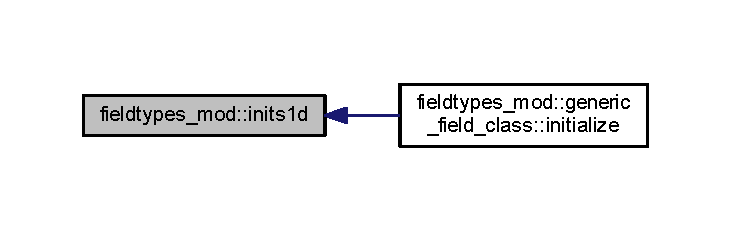
\includegraphics[width=350pt]{namespacefieldtypes__mod_a3f1571ad15733a3f2fff43e35f309416_icgraph}
\end{center}
\end{figure}
\mbox{\Hypertarget{namespacefieldtypes__mod_ad3329e97ec60bf9226d19be45ed21859}\label{namespacefieldtypes__mod_ad3329e97ec60bf9226d19be45ed21859}} 
\index{fieldtypes\+\_\+mod@{fieldtypes\+\_\+mod}!inits2d@{inits2d}}
\index{inits2d@{inits2d}!fieldtypes\+\_\+mod@{fieldtypes\+\_\+mod}}
\subsubsection{\texorpdfstring{inits2d()}{inits2d()}}
{\footnotesize\ttfamily subroutine fieldtypes\+\_\+mod\+::inits2d (\begin{DoxyParamCaption}\item[{class(\mbox{\hyperlink{structfieldtypes__mod_1_1generic__field__class}{generic\+\_\+field\+\_\+class}}), intent(inout)}]{self,  }\item[{type(string), intent(in)}]{name,  }\item[{type(string), intent(in)}]{units,  }\item[{real(prec), dimension(\+:,\+:), intent(in)}]{field }\end{DoxyParamCaption})\hspace{0.3cm}{\ttfamily [private]}}



Method that allocates and initializes a scalar 2D field in a generic field. 

\begin{DoxyAuthor}{Author}
Ricardo Birjukovs Canelas -\/ M\+A\+R\+E\+T\+EC 
\end{DoxyAuthor}

\begin{DoxyParams}[1]{Parameters}
\mbox{\tt in}  & {\em self,name,units,field} & \\
\hline
\end{DoxyParams}


Definition at line 369 of file fields\+Types.\+f90.


\begin{DoxyCode}
369     \textcolor{keywordtype}{class}(generic\_field\_class), \textcolor{keywordtype}{intent(inout)} :: self
370     \textcolor{keywordtype}{real(prec)}, \textcolor{keywordtype}{intent(in)}, \textcolor{keywordtype}{dimension(:,:)} :: field
371     \textcolor{keywordtype}{type}(string), \textcolor{keywordtype}{intent(in)} :: name
372     \textcolor{keywordtype}{type}(string), \textcolor{keywordtype}{intent(in)} :: units
373     \textcolor{keywordtype}{type}(string) :: outext
374     \textcolor{keywordflow}{if} (\textcolor{keyword}{allocated}(self%scalar2d%field)) \textcolor{keywordflow}{then}
375         outext = \textcolor{stringliteral}{'[generic\_field\_class::initialize]: scalar 2D field already allocated'}
376         \textcolor{keyword}{call }log%put(outext)
377         stop
378     \textcolor{keywordflow}{else}
379         \textcolor{keyword}{call }self%scalar2d%initialize(name, units, 2, field)
380         \textcolor{keyword}{call }self%setFieldMetadata(name, units, 2)
381 \textcolor{keywordflow}{    end if}
\end{DoxyCode}
Here is the caller graph for this function\+:\nopagebreak
\begin{figure}[H]
\begin{center}
\leavevmode
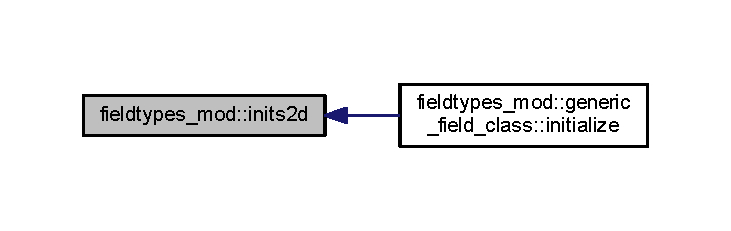
\includegraphics[width=350pt]{namespacefieldtypes__mod_ad3329e97ec60bf9226d19be45ed21859_icgraph}
\end{center}
\end{figure}
\mbox{\Hypertarget{namespacefieldtypes__mod_a750ce2c729d98ea7031c839a3a5ebd7c}\label{namespacefieldtypes__mod_a750ce2c729d98ea7031c839a3a5ebd7c}} 
\index{fieldtypes\+\_\+mod@{fieldtypes\+\_\+mod}!inits3d@{inits3d}}
\index{inits3d@{inits3d}!fieldtypes\+\_\+mod@{fieldtypes\+\_\+mod}}
\subsubsection{\texorpdfstring{inits3d()}{inits3d()}}
{\footnotesize\ttfamily subroutine fieldtypes\+\_\+mod\+::inits3d (\begin{DoxyParamCaption}\item[{class(\mbox{\hyperlink{structfieldtypes__mod_1_1generic__field__class}{generic\+\_\+field\+\_\+class}}), intent(inout)}]{self,  }\item[{type(string), intent(in)}]{name,  }\item[{type(string), intent(in)}]{units,  }\item[{real(prec), dimension(\+:,\+:,\+:), intent(in)}]{field }\end{DoxyParamCaption})\hspace{0.3cm}{\ttfamily [private]}}



Method that allocates and initializes a scalar 3D field in a generic field. 

\begin{DoxyAuthor}{Author}
Ricardo Birjukovs Canelas -\/ M\+A\+R\+E\+T\+EC 
\end{DoxyAuthor}

\begin{DoxyParams}[1]{Parameters}
\mbox{\tt in}  & {\em self,name,units,field} & \\
\hline
\end{DoxyParams}


Definition at line 391 of file fields\+Types.\+f90.


\begin{DoxyCode}
391     \textcolor{keywordtype}{class}(generic\_field\_class), \textcolor{keywordtype}{intent(inout)} :: self
392     \textcolor{keywordtype}{real(prec)}, \textcolor{keywordtype}{intent(in)}, \textcolor{keywordtype}{dimension(:,:,:)} :: field
393     \textcolor{keywordtype}{type}(string), \textcolor{keywordtype}{intent(in)} :: name
394     \textcolor{keywordtype}{type}(string), \textcolor{keywordtype}{intent(in)} :: units
395     \textcolor{keywordtype}{type}(string) :: outext
396     \textcolor{keywordflow}{if} (\textcolor{keyword}{allocated}(self%scalar3d%field)) \textcolor{keywordflow}{then}
397         outext = \textcolor{stringliteral}{'[generic\_field\_class::initialize]: scalar 3D field already allocated'}
398         \textcolor{keyword}{call }log%put(outext)
399         stop
400     \textcolor{keywordflow}{else}
401         \textcolor{keyword}{call }self%scalar3d%initialize(name, units, 3, field)
402         \textcolor{keyword}{call }self%setFieldMetadata(name, units, 3)
403 \textcolor{keywordflow}{    end if}
\end{DoxyCode}
Here is the caller graph for this function\+:\nopagebreak
\begin{figure}[H]
\begin{center}
\leavevmode
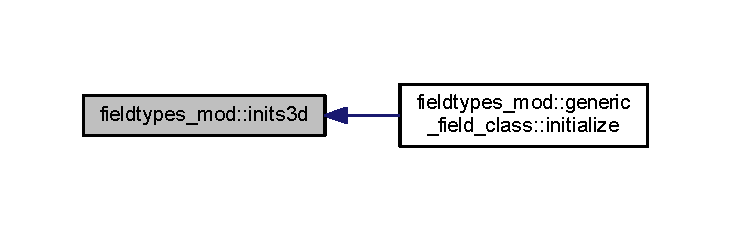
\includegraphics[width=350pt]{namespacefieldtypes__mod_a750ce2c729d98ea7031c839a3a5ebd7c_icgraph}
\end{center}
\end{figure}
\mbox{\Hypertarget{namespacefieldtypes__mod_a1987bd94293cfd9e35016ac5992501cd}\label{namespacefieldtypes__mod_a1987bd94293cfd9e35016ac5992501cd}} 
\index{fieldtypes\+\_\+mod@{fieldtypes\+\_\+mod}!inits4d@{inits4d}}
\index{inits4d@{inits4d}!fieldtypes\+\_\+mod@{fieldtypes\+\_\+mod}}
\subsubsection{\texorpdfstring{inits4d()}{inits4d()}}
{\footnotesize\ttfamily subroutine fieldtypes\+\_\+mod\+::inits4d (\begin{DoxyParamCaption}\item[{class(\mbox{\hyperlink{structfieldtypes__mod_1_1generic__field__class}{generic\+\_\+field\+\_\+class}}), intent(inout)}]{self,  }\item[{type(string), intent(in)}]{name,  }\item[{type(string), intent(in)}]{units,  }\item[{real(prec), dimension(\+:,\+:,\+:,\+:), intent(in)}]{field }\end{DoxyParamCaption})\hspace{0.3cm}{\ttfamily [private]}}



Method that allocates and initializes a scalar 4D field in a generic field. 

\begin{DoxyAuthor}{Author}
Ricardo Birjukovs Canelas -\/ M\+A\+R\+E\+T\+EC 
\end{DoxyAuthor}

\begin{DoxyParams}[1]{Parameters}
\mbox{\tt in}  & {\em self,name,units,field} & \\
\hline
\end{DoxyParams}


Definition at line 413 of file fields\+Types.\+f90.


\begin{DoxyCode}
413     \textcolor{keywordtype}{class}(generic\_field\_class), \textcolor{keywordtype}{intent(inout)} :: self
414     \textcolor{keywordtype}{real(prec)}, \textcolor{keywordtype}{intent(in)}, \textcolor{keywordtype}{dimension(:,:,:,:)} :: field
415     \textcolor{keywordtype}{type}(string), \textcolor{keywordtype}{intent(in)} :: name
416     \textcolor{keywordtype}{type}(string), \textcolor{keywordtype}{intent(in)} :: units
417     \textcolor{keywordtype}{type}(string) :: outext
418     \textcolor{keywordflow}{if} (\textcolor{keyword}{allocated}(self%scalar4d%field)) \textcolor{keywordflow}{then}
419         outext = \textcolor{stringliteral}{'[generic\_field\_class::initialize]: scalar 4D field already allocated'}
420         \textcolor{keyword}{call }log%put(outext)
421         stop
422     \textcolor{keywordflow}{else}
423         \textcolor{keyword}{call }self%scalar4d%initialize(name, units, 4, field)
424         \textcolor{keyword}{call }self%setFieldMetadata(name, units, 4)
425 \textcolor{keywordflow}{    end if}
\end{DoxyCode}
Here is the caller graph for this function\+:\nopagebreak
\begin{figure}[H]
\begin{center}
\leavevmode
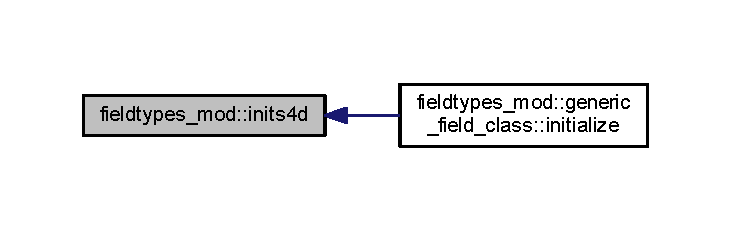
\includegraphics[width=350pt]{namespacefieldtypes__mod_a1987bd94293cfd9e35016ac5992501cd_icgraph}
\end{center}
\end{figure}
\mbox{\Hypertarget{namespacefieldtypes__mod_a96ff5318da6a7db8bb61c525315c1c89}\label{namespacefieldtypes__mod_a96ff5318da6a7db8bb61c525315c1c89}} 
\index{fieldtypes\+\_\+mod@{fieldtypes\+\_\+mod}!initscalar1dfield@{initscalar1dfield}}
\index{initscalar1dfield@{initscalar1dfield}!fieldtypes\+\_\+mod@{fieldtypes\+\_\+mod}}
\subsubsection{\texorpdfstring{initscalar1dfield()}{initscalar1dfield()}}
{\footnotesize\ttfamily subroutine fieldtypes\+\_\+mod\+::initscalar1dfield (\begin{DoxyParamCaption}\item[{class(\mbox{\hyperlink{structfieldtypes__mod_1_1scalar1d__field__class}{scalar1d\+\_\+field\+\_\+class}}), intent(inout)}]{self,  }\item[{type(string), intent(in)}]{name,  }\item[{type(string), intent(in)}]{units,  }\item[{integer, intent(in)}]{dim,  }\item[{real(prec), dimension(\+:), intent(in)}]{field }\end{DoxyParamCaption})\hspace{0.3cm}{\ttfamily [private]}}



Method that initializes a scalar 1D field. 

\begin{DoxyAuthor}{Author}
Ricardo Birjukovs Canelas -\/ M\+A\+R\+E\+T\+EC 
\end{DoxyAuthor}

\begin{DoxyParams}[1]{Parameters}
\mbox{\tt in}  & {\em self,name,units,dim,field} & \\
\hline
\end{DoxyParams}


Definition at line 501 of file fields\+Types.\+f90.


\begin{DoxyCode}
501     \textcolor{keywordtype}{class}(scalar1d\_field\_class), \textcolor{keywordtype}{intent(inout)} :: self
502     \textcolor{keywordtype}{real(prec)}, \textcolor{keywordtype}{intent(in)}, \textcolor{keywordtype}{dimension(:)} :: field
503     \textcolor{keywordtype}{type}(string), \textcolor{keywordtype}{intent(in)} :: name
504     \textcolor{keywordtype}{type}(string), \textcolor{keywordtype}{intent(in)} :: units
505     \textcolor{keywordtype}{integer}, \textcolor{keywordtype}{intent(in)} :: dim
506     \textcolor{keyword}{call }self%setFieldMetadata(name, units, dim)
507     \textcolor{keyword}{allocate}(self%field, source = field)
\end{DoxyCode}
\mbox{\Hypertarget{namespacefieldtypes__mod_a1a3160727c99017639d758aad9031df5}\label{namespacefieldtypes__mod_a1a3160727c99017639d758aad9031df5}} 
\index{fieldtypes\+\_\+mod@{fieldtypes\+\_\+mod}!initscalar2dfield@{initscalar2dfield}}
\index{initscalar2dfield@{initscalar2dfield}!fieldtypes\+\_\+mod@{fieldtypes\+\_\+mod}}
\subsubsection{\texorpdfstring{initscalar2dfield()}{initscalar2dfield()}}
{\footnotesize\ttfamily subroutine fieldtypes\+\_\+mod\+::initscalar2dfield (\begin{DoxyParamCaption}\item[{class(\mbox{\hyperlink{structfieldtypes__mod_1_1scalar2d__field__class}{scalar2d\+\_\+field\+\_\+class}}), intent(inout)}]{self,  }\item[{type(string), intent(in)}]{name,  }\item[{type(string), intent(in)}]{units,  }\item[{integer, intent(in)}]{dim,  }\item[{real(prec), dimension(\+:,\+:), intent(in)}]{field }\end{DoxyParamCaption})\hspace{0.3cm}{\ttfamily [private]}}



Method that initializes a scalar 2D field. 

\begin{DoxyAuthor}{Author}
Ricardo Birjukovs Canelas -\/ M\+A\+R\+E\+T\+EC 
\end{DoxyAuthor}

\begin{DoxyParams}[1]{Parameters}
\mbox{\tt in}  & {\em self,name,units,dim,field} & \\
\hline
\end{DoxyParams}


Definition at line 528 of file fields\+Types.\+f90.


\begin{DoxyCode}
528     \textcolor{keywordtype}{class}(scalar2d\_field\_class), \textcolor{keywordtype}{intent(inout)} :: self
529     \textcolor{keywordtype}{real(prec)}, \textcolor{keywordtype}{intent(in)}, \textcolor{keywordtype}{dimension(:,:)} :: field
530     \textcolor{keywordtype}{type}(string), \textcolor{keywordtype}{intent(in)} :: name
531     \textcolor{keywordtype}{type}(string), \textcolor{keywordtype}{intent(in)} :: units
532     \textcolor{keywordtype}{integer}, \textcolor{keywordtype}{intent(in)} :: dim
533     \textcolor{keyword}{call }self%setFieldMetadata(name, units, dim)
534     \textcolor{keyword}{allocate}(self%field, source = field)
\end{DoxyCode}
\mbox{\Hypertarget{namespacefieldtypes__mod_a3f2b90bc391ea5b84ead8069ee90f515}\label{namespacefieldtypes__mod_a3f2b90bc391ea5b84ead8069ee90f515}} 
\index{fieldtypes\+\_\+mod@{fieldtypes\+\_\+mod}!initscalar3dfield@{initscalar3dfield}}
\index{initscalar3dfield@{initscalar3dfield}!fieldtypes\+\_\+mod@{fieldtypes\+\_\+mod}}
\subsubsection{\texorpdfstring{initscalar3dfield()}{initscalar3dfield()}}
{\footnotesize\ttfamily subroutine fieldtypes\+\_\+mod\+::initscalar3dfield (\begin{DoxyParamCaption}\item[{class(\mbox{\hyperlink{structfieldtypes__mod_1_1scalar3d__field__class}{scalar3d\+\_\+field\+\_\+class}}), intent(inout)}]{self,  }\item[{type(string), intent(in)}]{name,  }\item[{type(string), intent(in)}]{units,  }\item[{integer, intent(in)}]{dim,  }\item[{real(prec), dimension(\+:,\+:,\+:), intent(in)}]{field }\end{DoxyParamCaption})\hspace{0.3cm}{\ttfamily [private]}}



Method that initializes a scalar 3D field. 

\begin{DoxyAuthor}{Author}
Ricardo Birjukovs Canelas -\/ M\+A\+R\+E\+T\+EC 
\end{DoxyAuthor}

\begin{DoxyParams}[1]{Parameters}
\mbox{\tt in}  & {\em self,name,units,dim,field} & \\
\hline
\end{DoxyParams}


Definition at line 555 of file fields\+Types.\+f90.


\begin{DoxyCode}
555     \textcolor{keywordtype}{class}(scalar3d\_field\_class), \textcolor{keywordtype}{intent(inout)} :: self
556     \textcolor{keywordtype}{real(prec)}, \textcolor{keywordtype}{intent(in)}, \textcolor{keywordtype}{dimension(:,:,:)} :: field
557     \textcolor{keywordtype}{type}(string), \textcolor{keywordtype}{intent(in)} :: name
558     \textcolor{keywordtype}{type}(string), \textcolor{keywordtype}{intent(in)} :: units
559     \textcolor{keywordtype}{integer}, \textcolor{keywordtype}{intent(in)} :: dim
560     \textcolor{keyword}{call }self%setFieldMetadata(name, units, dim)
561     \textcolor{keyword}{allocate}(self%field, source = field)
\end{DoxyCode}
\mbox{\Hypertarget{namespacefieldtypes__mod_a21dba84bb8fdb02d8bf5fd0052b51283}\label{namespacefieldtypes__mod_a21dba84bb8fdb02d8bf5fd0052b51283}} 
\index{fieldtypes\+\_\+mod@{fieldtypes\+\_\+mod}!initscalar4dfield@{initscalar4dfield}}
\index{initscalar4dfield@{initscalar4dfield}!fieldtypes\+\_\+mod@{fieldtypes\+\_\+mod}}
\subsubsection{\texorpdfstring{initscalar4dfield()}{initscalar4dfield()}}
{\footnotesize\ttfamily subroutine fieldtypes\+\_\+mod\+::initscalar4dfield (\begin{DoxyParamCaption}\item[{class(\mbox{\hyperlink{structfieldtypes__mod_1_1scalar4d__field__class}{scalar4d\+\_\+field\+\_\+class}}), intent(inout)}]{self,  }\item[{type(string), intent(in)}]{name,  }\item[{type(string), intent(in)}]{units,  }\item[{integer, intent(in)}]{dim,  }\item[{real(prec), dimension(\+:,\+:,\+:,\+:), intent(in)}]{field }\end{DoxyParamCaption})\hspace{0.3cm}{\ttfamily [private]}}



Method that initializes a scalar 4D field. 

\begin{DoxyAuthor}{Author}
Ricardo Birjukovs Canelas -\/ M\+A\+R\+E\+T\+EC 
\end{DoxyAuthor}

\begin{DoxyParams}[1]{Parameters}
\mbox{\tt in}  & {\em self,name,units,dim,field} & \\
\hline
\end{DoxyParams}


Definition at line 582 of file fields\+Types.\+f90.


\begin{DoxyCode}
582     \textcolor{keywordtype}{class}(scalar4d\_field\_class), \textcolor{keywordtype}{intent(inout)} :: self
583     \textcolor{keywordtype}{real(prec)}, \textcolor{keywordtype}{intent(in)}, \textcolor{keywordtype}{dimension(:,:,:,:)} :: field
584     \textcolor{keywordtype}{type}(string), \textcolor{keywordtype}{intent(in)} :: name
585     \textcolor{keywordtype}{type}(string), \textcolor{keywordtype}{intent(in)} :: units
586     \textcolor{keywordtype}{integer}, \textcolor{keywordtype}{intent(in)} :: dim
587     \textcolor{keyword}{call }self%setFieldMetadata(name, units, dim)
588     \textcolor{keyword}{allocate}(self%field, source = field)
\end{DoxyCode}
\mbox{\Hypertarget{namespacefieldtypes__mod_ad1af664e23793260f9c2fcd03829a1f5}\label{namespacefieldtypes__mod_ad1af664e23793260f9c2fcd03829a1f5}} 
\index{fieldtypes\+\_\+mod@{fieldtypes\+\_\+mod}!initv2d@{initv2d}}
\index{initv2d@{initv2d}!fieldtypes\+\_\+mod@{fieldtypes\+\_\+mod}}
\subsubsection{\texorpdfstring{initv2d()}{initv2d()}}
{\footnotesize\ttfamily subroutine fieldtypes\+\_\+mod\+::initv2d (\begin{DoxyParamCaption}\item[{class(\mbox{\hyperlink{structfieldtypes__mod_1_1generic__field__class}{generic\+\_\+field\+\_\+class}}), intent(inout)}]{self,  }\item[{type(string), intent(in)}]{name,  }\item[{type(string), intent(in)}]{units,  }\item[{type(vector), dimension(\+:,\+:), intent(in)}]{field }\end{DoxyParamCaption})\hspace{0.3cm}{\ttfamily [private]}}



Method that allocates and initializes a vectorial 2D field in a generic field. 

\begin{DoxyAuthor}{Author}
Ricardo Birjukovs Canelas -\/ M\+A\+R\+E\+T\+EC 
\end{DoxyAuthor}

\begin{DoxyParams}[1]{Parameters}
\mbox{\tt in}  & {\em self,name,units,field} & \\
\hline
\end{DoxyParams}


Definition at line 435 of file fields\+Types.\+f90.


\begin{DoxyCode}
435     \textcolor{keywordtype}{class}(generic\_field\_class), \textcolor{keywordtype}{intent(inout)} :: self
436     \textcolor{keywordtype}{type}(vector), \textcolor{keywordtype}{intent(in)}, \textcolor{keywordtype}{dimension(:,:)} :: field
437     \textcolor{keywordtype}{type}(string), \textcolor{keywordtype}{intent(in)} :: name
438     \textcolor{keywordtype}{type}(string), \textcolor{keywordtype}{intent(in)} :: units
439     \textcolor{keywordtype}{type}(string) :: outext
440     \textcolor{keywordflow}{if} (\textcolor{keyword}{allocated}(self%vectorial2d%field)) \textcolor{keywordflow}{then}
441         outext = \textcolor{stringliteral}{'[generic\_field\_class::initialize]: vectorial 2D field already allocated'}
442         \textcolor{keyword}{call }log%put(outext)
443         stop
444     \textcolor{keywordflow}{else}
445         \textcolor{keyword}{call }self%vectorial2d%initialize(name, units, 2, field)
446         \textcolor{keyword}{call }self%setFieldMetadata(name, units, 2)
447 \textcolor{keywordflow}{    end if}
\end{DoxyCode}
Here is the caller graph for this function\+:\nopagebreak
\begin{figure}[H]
\begin{center}
\leavevmode
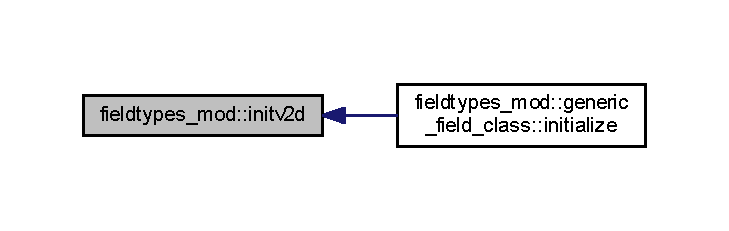
\includegraphics[width=350pt]{namespacefieldtypes__mod_ad1af664e23793260f9c2fcd03829a1f5_icgraph}
\end{center}
\end{figure}
\mbox{\Hypertarget{namespacefieldtypes__mod_aa0a152c9e5131d3003cc34e4f3b2974d}\label{namespacefieldtypes__mod_aa0a152c9e5131d3003cc34e4f3b2974d}} 
\index{fieldtypes\+\_\+mod@{fieldtypes\+\_\+mod}!initv3d@{initv3d}}
\index{initv3d@{initv3d}!fieldtypes\+\_\+mod@{fieldtypes\+\_\+mod}}
\subsubsection{\texorpdfstring{initv3d()}{initv3d()}}
{\footnotesize\ttfamily subroutine fieldtypes\+\_\+mod\+::initv3d (\begin{DoxyParamCaption}\item[{class(\mbox{\hyperlink{structfieldtypes__mod_1_1generic__field__class}{generic\+\_\+field\+\_\+class}}), intent(inout)}]{self,  }\item[{type(string), intent(in)}]{name,  }\item[{type(string), intent(in)}]{units,  }\item[{type(vector), dimension(\+:,\+:,\+:), intent(in)}]{field }\end{DoxyParamCaption})\hspace{0.3cm}{\ttfamily [private]}}



Method that allocates and initializes a vectorial 3D field in a generic field. 

\begin{DoxyAuthor}{Author}
Ricardo Birjukovs Canelas -\/ M\+A\+R\+E\+T\+EC 
\end{DoxyAuthor}

\begin{DoxyParams}[1]{Parameters}
\mbox{\tt in}  & {\em self,name,units,field} & \\
\hline
\end{DoxyParams}


Definition at line 457 of file fields\+Types.\+f90.


\begin{DoxyCode}
457     \textcolor{keywordtype}{class}(generic\_field\_class), \textcolor{keywordtype}{intent(inout)} :: self
458     \textcolor{keywordtype}{type}(vector), \textcolor{keywordtype}{intent(in)}, \textcolor{keywordtype}{dimension(:,:,:)} :: field
459     \textcolor{keywordtype}{type}(string), \textcolor{keywordtype}{intent(in)} :: name
460     \textcolor{keywordtype}{type}(string), \textcolor{keywordtype}{intent(in)} :: units
461     \textcolor{keywordtype}{type}(string) :: outext
462     \textcolor{keywordflow}{if} (\textcolor{keyword}{allocated}(self%vectorial3d%field)) \textcolor{keywordflow}{then}
463         outext = \textcolor{stringliteral}{'[generic\_field\_class::initialize]: vectorial 3D field already allocated'}
464         \textcolor{keyword}{call }log%put(outext)
465         stop
466     \textcolor{keywordflow}{else}
467         \textcolor{keyword}{call }self%vectorial3d%initialize(name, units, 3, field)
468         \textcolor{keyword}{call }self%setFieldMetadata(name, units, 3)
469 \textcolor{keywordflow}{    end if}
\end{DoxyCode}
Here is the caller graph for this function\+:\nopagebreak
\begin{figure}[H]
\begin{center}
\leavevmode
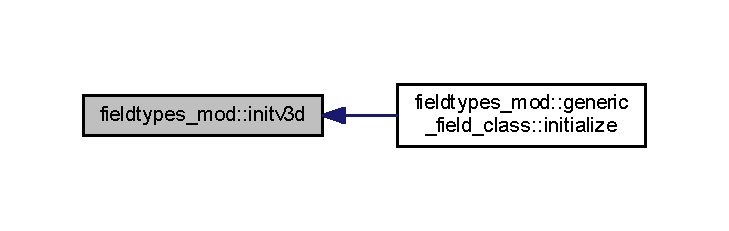
\includegraphics[width=350pt]{namespacefieldtypes__mod_aa0a152c9e5131d3003cc34e4f3b2974d_icgraph}
\end{center}
\end{figure}
\mbox{\Hypertarget{namespacefieldtypes__mod_a08d665678bea0956a323d08863e164e5}\label{namespacefieldtypes__mod_a08d665678bea0956a323d08863e164e5}} 
\index{fieldtypes\+\_\+mod@{fieldtypes\+\_\+mod}!initv4d@{initv4d}}
\index{initv4d@{initv4d}!fieldtypes\+\_\+mod@{fieldtypes\+\_\+mod}}
\subsubsection{\texorpdfstring{initv4d()}{initv4d()}}
{\footnotesize\ttfamily subroutine fieldtypes\+\_\+mod\+::initv4d (\begin{DoxyParamCaption}\item[{class(\mbox{\hyperlink{structfieldtypes__mod_1_1generic__field__class}{generic\+\_\+field\+\_\+class}}), intent(inout)}]{self,  }\item[{type(string), intent(in)}]{name,  }\item[{type(string), intent(in)}]{units,  }\item[{type(vector), dimension(\+:,\+:,\+:,\+:), intent(in)}]{field }\end{DoxyParamCaption})\hspace{0.3cm}{\ttfamily [private]}}



Method that allocates and initializes a vectorial 4D field in a generic field. 

\begin{DoxyAuthor}{Author}
Ricardo Birjukovs Canelas -\/ M\+A\+R\+E\+T\+EC 
\end{DoxyAuthor}

\begin{DoxyParams}[1]{Parameters}
\mbox{\tt in}  & {\em self,name,units,field} & \\
\hline
\end{DoxyParams}


Definition at line 479 of file fields\+Types.\+f90.


\begin{DoxyCode}
479     \textcolor{keywordtype}{class}(generic\_field\_class), \textcolor{keywordtype}{intent(inout)} :: self
480     \textcolor{keywordtype}{type}(vector), \textcolor{keywordtype}{intent(in)}, \textcolor{keywordtype}{dimension(:,:,:,:)} :: field
481     \textcolor{keywordtype}{type}(string), \textcolor{keywordtype}{intent(in)} :: name
482     \textcolor{keywordtype}{type}(string), \textcolor{keywordtype}{intent(in)} :: units
483     \textcolor{keywordtype}{type}(string) :: outext
484     \textcolor{keywordflow}{if} (\textcolor{keyword}{allocated}(self%vectorial4d%field)) \textcolor{keywordflow}{then}
485         outext = \textcolor{stringliteral}{'[generic\_field\_class::initialize]: vectorial 4D field already allocated'}
486         \textcolor{keyword}{call }log%put(outext)
487         stop
488     \textcolor{keywordflow}{else}
489         \textcolor{keyword}{call }self%vectorial4d%initialize(name, units, 4, field)
490         \textcolor{keyword}{call }self%setFieldMetadata(name, units, 4)
491 \textcolor{keywordflow}{    end if}
\end{DoxyCode}
Here is the caller graph for this function\+:\nopagebreak
\begin{figure}[H]
\begin{center}
\leavevmode
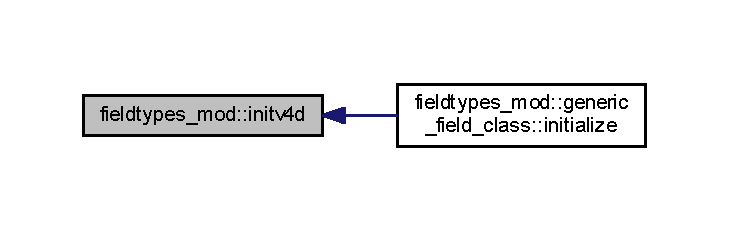
\includegraphics[width=350pt]{namespacefieldtypes__mod_a08d665678bea0956a323d08863e164e5_icgraph}
\end{center}
\end{figure}
\mbox{\Hypertarget{namespacefieldtypes__mod_ac3e3d9aabba3893d61583e890e3bdf41}\label{namespacefieldtypes__mod_ac3e3d9aabba3893d61583e890e3bdf41}} 
\index{fieldtypes\+\_\+mod@{fieldtypes\+\_\+mod}!initvectorial2dfield@{initvectorial2dfield}}
\index{initvectorial2dfield@{initvectorial2dfield}!fieldtypes\+\_\+mod@{fieldtypes\+\_\+mod}}
\subsubsection{\texorpdfstring{initvectorial2dfield()}{initvectorial2dfield()}}
{\footnotesize\ttfamily subroutine fieldtypes\+\_\+mod\+::initvectorial2dfield (\begin{DoxyParamCaption}\item[{class(\mbox{\hyperlink{structfieldtypes__mod_1_1vectorial2d__field__class}{vectorial2d\+\_\+field\+\_\+class}}), intent(inout)}]{self,  }\item[{type(string), intent(in)}]{name,  }\item[{type(string), intent(in)}]{units,  }\item[{integer, intent(in)}]{dim,  }\item[{type(vector), dimension(\+:,\+:), intent(in)}]{field }\end{DoxyParamCaption})\hspace{0.3cm}{\ttfamily [private]}}



Method that initializes a vectorial 2D field. 

\begin{DoxyAuthor}{Author}
Ricardo Birjukovs Canelas -\/ M\+A\+R\+E\+T\+EC 
\end{DoxyAuthor}

\begin{DoxyParams}[1]{Parameters}
\mbox{\tt in}  & {\em self,name,units,dim,field} & \\
\hline
\end{DoxyParams}


Definition at line 609 of file fields\+Types.\+f90.


\begin{DoxyCode}
609     \textcolor{keywordtype}{class}(vectorial2d\_field\_class), \textcolor{keywordtype}{intent(inout)} :: self
610     \textcolor{keywordtype}{type}(vector), \textcolor{keywordtype}{intent(in)}, \textcolor{keywordtype}{dimension(:,:)} :: field
611     \textcolor{keywordtype}{type}(string), \textcolor{keywordtype}{intent(in)} :: name
612     \textcolor{keywordtype}{type}(string), \textcolor{keywordtype}{intent(in)} :: units
613     \textcolor{keywordtype}{integer}, \textcolor{keywordtype}{intent(in)} :: dim
614     \textcolor{keyword}{call }self%setFieldMetadata(name, units, dim)
615     \textcolor{keyword}{allocate}(self%field, source = field)
\end{DoxyCode}
\mbox{\Hypertarget{namespacefieldtypes__mod_a20d935cfa1513350667d04f969be5e26}\label{namespacefieldtypes__mod_a20d935cfa1513350667d04f969be5e26}} 
\index{fieldtypes\+\_\+mod@{fieldtypes\+\_\+mod}!initvectorial3dfield@{initvectorial3dfield}}
\index{initvectorial3dfield@{initvectorial3dfield}!fieldtypes\+\_\+mod@{fieldtypes\+\_\+mod}}
\subsubsection{\texorpdfstring{initvectorial3dfield()}{initvectorial3dfield()}}
{\footnotesize\ttfamily subroutine fieldtypes\+\_\+mod\+::initvectorial3dfield (\begin{DoxyParamCaption}\item[{class(\mbox{\hyperlink{structfieldtypes__mod_1_1vectorial3d__field__class}{vectorial3d\+\_\+field\+\_\+class}}), intent(inout)}]{self,  }\item[{type(string), intent(in)}]{name,  }\item[{type(string), intent(in)}]{units,  }\item[{integer, intent(in)}]{dim,  }\item[{type(vector), dimension(\+:,\+:,\+:), intent(in)}]{field }\end{DoxyParamCaption})\hspace{0.3cm}{\ttfamily [private]}}



Method that initializes a vectorial 3D field. 

\begin{DoxyAuthor}{Author}
Ricardo Birjukovs Canelas -\/ M\+A\+R\+E\+T\+EC 
\end{DoxyAuthor}

\begin{DoxyParams}[1]{Parameters}
\mbox{\tt in}  & {\em self,name,units,dim,field} & \\
\hline
\end{DoxyParams}


Definition at line 625 of file fields\+Types.\+f90.


\begin{DoxyCode}
625     \textcolor{keywordtype}{class}(vectorial3d\_field\_class), \textcolor{keywordtype}{intent(inout)} :: self
626     \textcolor{keywordtype}{type}(vector), \textcolor{keywordtype}{intent(in)}, \textcolor{keywordtype}{dimension(:,:,:)} :: field
627     \textcolor{keywordtype}{type}(string), \textcolor{keywordtype}{intent(in)} :: name
628     \textcolor{keywordtype}{type}(string), \textcolor{keywordtype}{intent(in)} :: units
629     \textcolor{keywordtype}{integer}, \textcolor{keywordtype}{intent(in)} :: dim
630     \textcolor{keyword}{call }self%setFieldMetadata(name, units, dim)
631     \textcolor{keyword}{allocate}(self%field, source = field)
\end{DoxyCode}
\mbox{\Hypertarget{namespacefieldtypes__mod_ad458710e4a2d6c40a3dfa7f19481cd5a}\label{namespacefieldtypes__mod_ad458710e4a2d6c40a3dfa7f19481cd5a}} 
\index{fieldtypes\+\_\+mod@{fieldtypes\+\_\+mod}!initvectorial4dfield@{initvectorial4dfield}}
\index{initvectorial4dfield@{initvectorial4dfield}!fieldtypes\+\_\+mod@{fieldtypes\+\_\+mod}}
\subsubsection{\texorpdfstring{initvectorial4dfield()}{initvectorial4dfield()}}
{\footnotesize\ttfamily subroutine fieldtypes\+\_\+mod\+::initvectorial4dfield (\begin{DoxyParamCaption}\item[{class(\mbox{\hyperlink{structfieldtypes__mod_1_1vectorial4d__field__class}{vectorial4d\+\_\+field\+\_\+class}}), intent(inout)}]{self,  }\item[{type(string), intent(in)}]{name,  }\item[{type(string), intent(in)}]{units,  }\item[{integer, intent(in)}]{dim,  }\item[{type(vector), dimension(\+:,\+:,\+:,\+:), intent(in)}]{field }\end{DoxyParamCaption})\hspace{0.3cm}{\ttfamily [private]}}



Method that initializes a vectorial 4D field. 

\begin{DoxyAuthor}{Author}
Ricardo Birjukovs Canelas -\/ M\+A\+R\+E\+T\+EC 
\end{DoxyAuthor}

\begin{DoxyParams}[1]{Parameters}
\mbox{\tt in}  & {\em self,name,units,dim,field} & \\
\hline
\end{DoxyParams}


Definition at line 641 of file fields\+Types.\+f90.


\begin{DoxyCode}
641     \textcolor{keywordtype}{class}(vectorial4d\_field\_class), \textcolor{keywordtype}{intent(inout)} :: self
642     \textcolor{keywordtype}{type}(vector), \textcolor{keywordtype}{intent(in)}, \textcolor{keywordtype}{dimension(:,:,:,:)} :: field
643     \textcolor{keywordtype}{type}(string), \textcolor{keywordtype}{intent(in)} :: name
644     \textcolor{keywordtype}{type}(string), \textcolor{keywordtype}{intent(in)} :: units
645     \textcolor{keywordtype}{integer}, \textcolor{keywordtype}{intent(in)} :: dim
646     \textcolor{keyword}{call }self%setFieldMetadata(name, units, dim)
647     \textcolor{keyword}{allocate}(self%field, source = field)
\end{DoxyCode}
\mbox{\Hypertarget{namespacefieldtypes__mod_a5a556fba603c1d39b20713fdbc813332}\label{namespacefieldtypes__mod_a5a556fba603c1d39b20713fdbc813332}} 
\index{fieldtypes\+\_\+mod@{fieldtypes\+\_\+mod}!printfield@{printfield}}
\index{printfield@{printfield}!fieldtypes\+\_\+mod@{fieldtypes\+\_\+mod}}
\subsubsection{\texorpdfstring{printfield()}{printfield()}}
{\footnotesize\ttfamily subroutine fieldtypes\+\_\+mod\+::printfield (\begin{DoxyParamCaption}\item[{class(\mbox{\hyperlink{structfieldtypes__mod_1_1field__class}{field\+\_\+class}}), intent(in)}]{self }\end{DoxyParamCaption})\hspace{0.3cm}{\ttfamily [private]}}



Method that prints the field information. 

\begin{DoxyAuthor}{Author}
Ricardo Birjukovs Canelas -\/ M\+A\+R\+E\+T\+EC 
\end{DoxyAuthor}


Definition at line 736 of file fields\+Types.\+f90.


\begin{DoxyCode}
736     \textcolor{keywordtype}{class}(field\_class), \textcolor{keywordtype}{intent(in)} :: self
737     \textcolor{keywordtype}{type}(string) :: outext, t(5)
738     t(1) = self%dim
739     t(2) = self%getFieldType()
740     t(3) = self%getFieldMinBound()
741     t(4) = self%getFieldMaxBound()
742     \textcolor{comment}{!t(5) = self%getFieldShape()}
743     outext = t(2)//\textcolor{stringliteral}{' field['}//self%name//\textcolor{stringliteral}{'] has dimensionality '}//t(1)//\textcolor{stringliteral}{' and is in '}//self%units//\textcolor{stringliteral}{' - ['}//
      t(3)//\textcolor{stringliteral}{';'}//t(4)//\textcolor{stringliteral}{']'}\textcolor{comment}{!, ('//t(5)//')'}
744     \textcolor{keyword}{call }log%put(outext,.false.)
\end{DoxyCode}
\mbox{\Hypertarget{namespacefieldtypes__mod_a63d399d72fffde3fe8169b76cce59259}\label{namespacefieldtypes__mod_a63d399d72fffde3fe8169b76cce59259}} 
\index{fieldtypes\+\_\+mod@{fieldtypes\+\_\+mod}!printgenericfield@{printgenericfield}}
\index{printgenericfield@{printgenericfield}!fieldtypes\+\_\+mod@{fieldtypes\+\_\+mod}}
\subsubsection{\texorpdfstring{printgenericfield()}{printgenericfield()}}
{\footnotesize\ttfamily subroutine fieldtypes\+\_\+mod\+::printgenericfield (\begin{DoxyParamCaption}\item[{class(\mbox{\hyperlink{structfieldtypes__mod_1_1generic__field__class}{generic\+\_\+field\+\_\+class}}), intent(in)}]{self }\end{DoxyParamCaption})\hspace{0.3cm}{\ttfamily [private]}}



Method that prints the generic field information. 

\begin{DoxyAuthor}{Author}
Ricardo Birjukovs Canelas -\/ M\+A\+R\+E\+T\+EC 
\end{DoxyAuthor}


Definition at line 673 of file fields\+Types.\+f90.


\begin{DoxyCode}
673     \textcolor{keywordtype}{class}(generic\_field\_class), \textcolor{keywordtype}{intent(in)} :: self
674     \textcolor{keywordflow}{if} (\textcolor{keyword}{allocated}(self%scalar1d%field)) \textcolor{keyword}{call }self%scalar1d%print()
675     \textcolor{keywordflow}{if} (\textcolor{keyword}{allocated}(self%scalar2d%field)) \textcolor{keyword}{call }self%scalar2d%print()
676     \textcolor{keywordflow}{if} (\textcolor{keyword}{allocated}(self%scalar3d%field)) \textcolor{keyword}{call }self%scalar3d%print()
677     \textcolor{keywordflow}{if} (\textcolor{keyword}{allocated}(self%scalar4d%field)) \textcolor{keyword}{call }self%scalar4d%print()
678     \textcolor{keywordflow}{if} (\textcolor{keyword}{allocated}(self%vectorial2d%field)) \textcolor{keyword}{call }self%vectorial2d%print()
679     \textcolor{keywordflow}{if} (\textcolor{keyword}{allocated}(self%vectorial3d%field)) \textcolor{keyword}{call }self%vectorial3d%print()
680     \textcolor{keywordflow}{if} (\textcolor{keyword}{allocated}(self%vectorial4d%field)) \textcolor{keyword}{call }self%vectorial4d%print()
\end{DoxyCode}
\mbox{\Hypertarget{namespacefieldtypes__mod_ad8f3bf57dafb3eac18e5a3198e36047c}\label{namespacefieldtypes__mod_ad8f3bf57dafb3eac18e5a3198e36047c}} 
\index{fieldtypes\+\_\+mod@{fieldtypes\+\_\+mod}!replacemetadata@{replacemetadata}}
\index{replacemetadata@{replacemetadata}!fieldtypes\+\_\+mod@{fieldtypes\+\_\+mod}}
\subsubsection{\texorpdfstring{replacemetadata()}{replacemetadata()}}
{\footnotesize\ttfamily subroutine fieldtypes\+\_\+mod\+::replacemetadata (\begin{DoxyParamCaption}\item[{class(\mbox{\hyperlink{structfieldtypes__mod_1_1generic__field__class}{generic\+\_\+field\+\_\+class}}), intent(inout)}]{self,  }\item[{type(string), intent(in)}]{name,  }\item[{type(string), intent(in)}]{units }\end{DoxyParamCaption})\hspace{0.3cm}{\ttfamily [private]}}



replaces metadata on a generic field 

\begin{DoxyAuthor}{Author}
Ricardo Birjukovs Canelas -\/ M\+A\+R\+E\+T\+EC 
\end{DoxyAuthor}

\begin{DoxyParams}[1]{Parameters}
\mbox{\tt in}  & {\em self,name,units} & \\
\hline
\end{DoxyParams}


Definition at line 284 of file fields\+Types.\+f90.


\begin{DoxyCode}
284     \textcolor{keywordtype}{class}(generic\_field\_class), \textcolor{keywordtype}{intent(inout)} :: self
285     \textcolor{keywordtype}{type}(string), \textcolor{keywordtype}{intent(in)} :: name
286     \textcolor{keywordtype}{type}(string), \textcolor{keywordtype}{intent(in)} :: units
287     self%name = name
288     self%units = units
\end{DoxyCode}
\mbox{\Hypertarget{namespacefieldtypes__mod_abc601ce9f8a974f426e876cc4c02e2a2}\label{namespacefieldtypes__mod_abc601ce9f8a974f426e876cc4c02e2a2}} 
\index{fieldtypes\+\_\+mod@{fieldtypes\+\_\+mod}!setfieldmetadata@{setfieldmetadata}}
\index{setfieldmetadata@{setfieldmetadata}!fieldtypes\+\_\+mod@{fieldtypes\+\_\+mod}}
\subsubsection{\texorpdfstring{setfieldmetadata()}{setfieldmetadata()}}
{\footnotesize\ttfamily subroutine fieldtypes\+\_\+mod\+::setfieldmetadata (\begin{DoxyParamCaption}\item[{class(\mbox{\hyperlink{structfieldtypes__mod_1_1field__class}{field\+\_\+class}}), intent(inout)}]{self,  }\item[{type(string), intent(in)}]{name,  }\item[{type(string), intent(in)}]{units,  }\item[{integer, intent(in)}]{dim }\end{DoxyParamCaption})\hspace{0.3cm}{\ttfamily [private]}}



Method that initializes a base field object by filling metadata. 

\begin{DoxyAuthor}{Author}
Ricardo Birjukovs Canelas -\/ M\+A\+R\+E\+T\+EC 
\end{DoxyAuthor}

\begin{DoxyParams}[1]{Parameters}
\mbox{\tt in}  & {\em self,name,units,dim} & \\
\hline
\end{DoxyParams}


Definition at line 658 of file fields\+Types.\+f90.


\begin{DoxyCode}
658     \textcolor{keywordtype}{class}(field\_class), \textcolor{keywordtype}{intent(inout)} :: self
659     \textcolor{keywordtype}{type}(string), \textcolor{keywordtype}{intent(in)} :: name
660     \textcolor{keywordtype}{type}(string), \textcolor{keywordtype}{intent(in)} :: units
661     \textcolor{keywordtype}{integer}, \textcolor{keywordtype}{intent(in)} :: dim
662     self%name = name
663     self%units = units
664     self%dim = dim
\end{DoxyCode}
\mbox{\Hypertarget{namespacefieldtypes__mod_a0babd6327ed77199d5437d17de34bafe}\label{namespacefieldtypes__mod_a0babd6327ed77199d5437d17de34bafe}} 
\index{fieldtypes\+\_\+mod@{fieldtypes\+\_\+mod}!test@{test}}
\index{test@{test}!fieldtypes\+\_\+mod@{fieldtypes\+\_\+mod}}
\subsubsection{\texorpdfstring{test()}{test()}}
{\footnotesize\ttfamily subroutine fieldtypes\+\_\+mod\+::test (\begin{DoxyParamCaption}\item[{class(\mbox{\hyperlink{structfieldtypes__mod_1_1generic__field__class}{generic\+\_\+field\+\_\+class}}), intent(inout)}]{self }\end{DoxyParamCaption})\hspace{0.3cm}{\ttfamily [private]}}



A class \textquotesingle{}unit\textquotesingle{} test for the \mbox{\hyperlink{structfieldtypes__mod_1_1generic__field__class}{generic\+\_\+field\+\_\+class}}. 

\begin{DoxyAuthor}{Author}
Ricardo Birjukovs Canelas -\/ M\+A\+R\+E\+T\+EC 
\end{DoxyAuthor}


Definition at line 706 of file fields\+Types.\+f90.


\begin{DoxyCode}
706     \textcolor{keywordtype}{class}(generic\_field\_class), \textcolor{keywordtype}{intent(inout)} :: self
707     \textcolor{keywordtype}{type}(generic\_field\_class) :: gfield1, gfield2, gfield3
708     \textcolor{keywordtype}{real(prec)}, \textcolor{keywordtype}{allocatable}, \textcolor{keywordtype}{dimension(:)} :: field1
709     \textcolor{keywordtype}{real(prec)}, \textcolor{keywordtype}{allocatable}, \textcolor{keywordtype}{dimension(:,:)} :: field2
710     \textcolor{keywordtype}{type}(vector), \textcolor{keywordtype}{allocatable}, \textcolor{keywordtype}{dimension(:,:,:)} :: field3
711     \textcolor{keywordtype}{type}(string) :: name1, name2, name3
712     \textcolor{keywordtype}{type}(string) :: units1, units2, units3
713     \textcolor{keyword}{allocate}(field1(50))
714     \textcolor{keyword}{allocate}(field2(20,60))
715     \textcolor{keyword}{allocate}(field3(2,3,4))
716     name1 = \textcolor{stringliteral}{'testfield1d'}
717     name2 = \textcolor{stringliteral}{'testfield2d'}
718     name3 = \textcolor{stringliteral}{'testfield3d'}
719     units1 = \textcolor{stringliteral}{'m/s'}
720     units2 = \textcolor{stringliteral}{'km'}
721     units3 = \textcolor{stringliteral}{'ms-1'}
722     \textcolor{keyword}{call }gfield1%initialize(name1, units1, field1)
723     \textcolor{keyword}{call }gfield2%initialize(name2, units2, field2)
724     \textcolor{keyword}{call }gfield3%initialize(name3, units3, field3)
725     \textcolor{keyword}{call }gfield1%print()
726     \textcolor{keyword}{call }gfield2%print()
727     \textcolor{keyword}{call }gfield3%print()
\end{DoxyCode}

\hypertarget{namespacegeometry__mod}{}\section{geometry\+\_\+mod Module Reference}
\label{namespacegeometry__mod}\index{geometry\+\_\+mod@{geometry\+\_\+mod}}


Module that defines geometry classes and related methods.  


\subsection*{Data Types}
\begin{DoxyCompactItemize}
\item 
type \mbox{\hyperlink{structgeometry__mod_1_1box}{box}}
\begin{DoxyCompactList}\small\item\em Type -\/ point class. \end{DoxyCompactList}\item 
type \mbox{\hyperlink{structgeometry__mod_1_1geometry__class}{geometry\+\_\+class}}
\item 
type \mbox{\hyperlink{structgeometry__mod_1_1line}{line}}
\begin{DoxyCompactList}\small\item\em Type -\/ line class. \end{DoxyCompactList}\item 
type \mbox{\hyperlink{structgeometry__mod_1_1point}{point}}
\begin{DoxyCompactList}\small\item\em Type -\/ point class. \end{DoxyCompactList}\item 
type \mbox{\hyperlink{structgeometry__mod_1_1shape}{shape}}
\begin{DoxyCompactList}\small\item\em Type -\/ extendable shape class. \end{DoxyCompactList}\item 
type \mbox{\hyperlink{structgeometry__mod_1_1sphere}{sphere}}
\begin{DoxyCompactList}\small\item\em Type -\/ sphere class. \end{DoxyCompactList}\end{DoxyCompactItemize}
\subsection*{Functions/\+Subroutines}
\begin{DoxyCompactItemize}
\item 
subroutine \mbox{\hyperlink{namespacegeometry__mod_a1b6f259b0b6be71e02ffae7670f7d8ba}{allocatelist}} (self)
\begin{DoxyCompactList}\small\item\em Public routine to allocate the possible geometry name list. \end{DoxyCompactList}\item 
logical function \mbox{\hyperlink{namespacegeometry__mod_a22dd77024fce56da299445a697256155}{inlist}} (self, geomname)
\begin{DoxyCompactList}\small\item\em Public function that returns a logical if the input geometry name is valid. \end{DoxyCompactList}\item 
integer function \mbox{\hyperlink{namespacegeometry__mod_ad790edd694561b33dad20cfa3a14e8f2}{fillsize}} (self, shapetype, dp)
\begin{DoxyCompactList}\small\item\em method to get the number of points that fill a given geometry \end{DoxyCompactList}\item 
subroutine \mbox{\hyperlink{namespacegeometry__mod_a1d97564e04562532b5389bfb91aa676b}{fill}} (self, shapetype, dp, \mbox{\hyperlink{namespacegeometry__mod_ad790edd694561b33dad20cfa3a14e8f2}{fillsize}}, ptlist)
\begin{DoxyCompactList}\small\item\em method to get the list of points that fill a given geometry \end{DoxyCompactList}\item 
type(vector) function \mbox{\hyperlink{namespacegeometry__mod_a4a38edbff02aa0ff5f16a16c39bf778e}{getcenter}} (self, shapetype)
\begin{DoxyCompactList}\small\item\em method to get the baricenter of a given geometry \end{DoxyCompactList}\item 
type(vector) function, dimension(\+:), allocatable \mbox{\hyperlink{namespacegeometry__mod_a0b1a3c5aa414292ace34d59487082e3a}{getpoints}} (self, shapetype)
\begin{DoxyCompactList}\small\item\em method that returns the points defining a given geometry \end{DoxyCompactList}\item 
integer function \mbox{\hyperlink{namespacegeometry__mod_a524c5d28a80fb6729b102126485605ce}{getnumpoints}} (self, shapetype)
\begin{DoxyCompactList}\small\item\em method the points defining a given geometry \end{DoxyCompactList}\item 
subroutine \mbox{\hyperlink{namespacegeometry__mod_aed4426181ca851b41717edd50268e5f3}{printgeometry}} (self, shapetype)
\begin{DoxyCompactList}\small\item\em method to print the details of a given geometry \end{DoxyCompactList}\item 
integer function \mbox{\hyperlink{namespacegeometry__mod_a05de7940b4e7df5a2b31f3d0414e3743}{sphere\+\_\+np\+\_\+count}} (dp, r)
\begin{DoxyCompactList}\small\item\em private function that returns the number of points distributed on a grid with spacing dp inside a sphere \end{DoxyCompactList}\item 
subroutine \mbox{\hyperlink{namespacegeometry__mod_a6c03a4ea3de6763940396dbeb3908ebc}{sphere\+\_\+grid}} (dp, r, np, ptlist)
\begin{DoxyCompactList}\small\item\em private routine that returns the points distributed on a grid with spacing dp inside a sphere \end{DoxyCompactList}\item 
subroutine \mbox{\hyperlink{namespacegeometry__mod_ae87e4ecff2d21a839da2b82919b5fd0b}{box\+\_\+grid}} (dp, size, np, ptlist)
\begin{DoxyCompactList}\small\item\em private routine that returns the points distributed on a grid with spacing dp inside a box \end{DoxyCompactList}\item 
subroutine \mbox{\hyperlink{namespacegeometry__mod_abcb09c0f5274c27cb79b0dd009ed94b3}{line\+\_\+grid}} (dp, dist, np, ptlist)
\begin{DoxyCompactList}\small\item\em private routine that returns the points distributed on a grid with spacing dp along a line \end{DoxyCompactList}\end{DoxyCompactItemize}
\subsection*{Variables}
\begin{DoxyCompactItemize}
\item 
type(\mbox{\hyperlink{structgeometry__mod_1_1geometry__class}{geometry\+\_\+class}}), public \mbox{\hyperlink{namespacegeometry__mod_ad2ad4f7e1138beaad5f37d5c15b7b457}{geometry}}
\end{DoxyCompactItemize}


\subsection{Detailed Description}
Module that defines geometry classes and related methods. 

\begin{DoxyAuthor}{Author}
Ricardo Birjukovs Canelas 
\end{DoxyAuthor}


\subsection{Function/\+Subroutine Documentation}
\mbox{\Hypertarget{namespacegeometry__mod_a1b6f259b0b6be71e02ffae7670f7d8ba}\label{namespacegeometry__mod_a1b6f259b0b6be71e02ffae7670f7d8ba}} 
\index{geometry\+\_\+mod@{geometry\+\_\+mod}!allocatelist@{allocatelist}}
\index{allocatelist@{allocatelist}!geometry\+\_\+mod@{geometry\+\_\+mod}}
\subsubsection{\texorpdfstring{allocatelist()}{allocatelist()}}
{\footnotesize\ttfamily subroutine geometry\+\_\+mod\+::allocatelist (\begin{DoxyParamCaption}\item[{class(\mbox{\hyperlink{structgeometry__mod_1_1geometry__class}{geometry\+\_\+class}}), intent(inout)}]{self }\end{DoxyParamCaption})\hspace{0.3cm}{\ttfamily [private]}}



Public routine to allocate the possible geometry name list. 

\begin{DoxyAuthor}{Author}
Ricardo Birjukovs Canelas -\/ M\+A\+R\+E\+T\+EC 
\end{DoxyAuthor}


Definition at line 79 of file geometry.\+f90.


\begin{DoxyCode}
79     \textcolor{keywordtype}{implicit none}
80     \textcolor{keywordtype}{class}(geometry\_class), \textcolor{keywordtype}{intent(inout)} :: self
81     \textcolor{keyword}{allocate}(self%list(4))
82     self%list(1) =\textcolor{stringliteral}{'point'}
83     self%list(2) =\textcolor{stringliteral}{'line'}
84     self%list(3) =\textcolor{stringliteral}{'box'}
85     self%list(4) =\textcolor{stringliteral}{'sphere'}
\end{DoxyCode}
\mbox{\Hypertarget{namespacegeometry__mod_ae87e4ecff2d21a839da2b82919b5fd0b}\label{namespacegeometry__mod_ae87e4ecff2d21a839da2b82919b5fd0b}} 
\index{geometry\+\_\+mod@{geometry\+\_\+mod}!box\+\_\+grid@{box\+\_\+grid}}
\index{box\+\_\+grid@{box\+\_\+grid}!geometry\+\_\+mod@{geometry\+\_\+mod}}
\subsubsection{\texorpdfstring{box\+\_\+grid()}{box\_grid()}}
{\footnotesize\ttfamily subroutine geometry\+\_\+mod\+::box\+\_\+grid (\begin{DoxyParamCaption}\item[{real(prec), intent(in)}]{dp,  }\item[{type(vector), intent(in)}]{size,  }\item[{integer, intent(in)}]{np,  }\item[{type(vector), dimension(np), intent(out)}]{ptlist }\end{DoxyParamCaption})\hspace{0.3cm}{\ttfamily [private]}}



private routine that returns the points distributed on a grid with spacing dp inside a box 

\begin{DoxyAuthor}{Author}
Ricardo Birjukovs Canelas -\/ M\+A\+R\+E\+T\+EC 
\end{DoxyAuthor}

\begin{DoxyParams}[1]{Parameters}
\mbox{\tt in}  & {\em dp,size,np,ptlist} & \\
\hline
\end{DoxyParams}


Definition at line 397 of file geometry.\+f90.


\begin{DoxyCode}
397     \textcolor{keywordtype}{implicit none}
398     \textcolor{keywordtype}{real(prec)}, \textcolor{keywordtype}{intent(in)} :: dp
399     \textcolor{keywordtype}{type}(vector), \textcolor{keywordtype}{intent(in)} :: size
400     \textcolor{keywordtype}{integer}, \textcolor{keywordtype}{intent(in)}::  np
401     \textcolor{keywordtype}{type}(vector), \textcolor{keywordtype}{intent(out)} :: ptlist(np)
402     \textcolor{keywordtype}{integer} :: i, j, k, p
403     p=0
404     \textcolor{keywordflow}{do} i=1, int(size%x/dp)+1
405         \textcolor{keywordflow}{do} j=1, int(size%y/dp)+1
406             \textcolor{keywordflow}{do} k=1, int(size%z/dp)+1
407                 p=p+1
408                 ptlist(p) = dp*(ex*(i-1) + ey*(j-1) + ez*(k-1))
409 \textcolor{keywordflow}{            end do}
410 \textcolor{keywordflow}{        end do}
411 \textcolor{keywordflow}{    end do}
412     \textcolor{keywordflow}{if} (np == 1) \textcolor{keywordflow}{then} \textcolor{comment}{!Just the origin}
413         ptlist(1)= 0*ex + 0*ey +0*ez
414 \textcolor{keywordflow}{    end if}
\end{DoxyCode}
Here is the caller graph for this function\+:\nopagebreak
\begin{figure}[H]
\begin{center}
\leavevmode
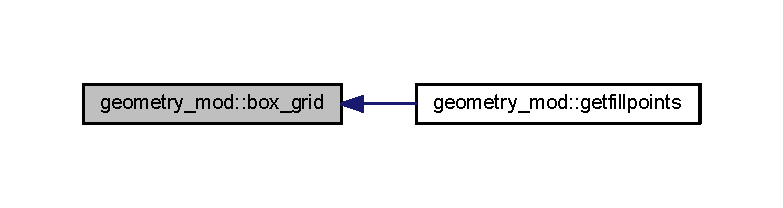
\includegraphics[width=336pt]{namespacegeometry__mod_ae87e4ecff2d21a839da2b82919b5fd0b_icgraph}
\end{center}
\end{figure}
\mbox{\Hypertarget{namespacegeometry__mod_a1d97564e04562532b5389bfb91aa676b}\label{namespacegeometry__mod_a1d97564e04562532b5389bfb91aa676b}} 
\index{geometry\+\_\+mod@{geometry\+\_\+mod}!fill@{fill}}
\index{fill@{fill}!geometry\+\_\+mod@{geometry\+\_\+mod}}
\subsubsection{\texorpdfstring{fill()}{fill()}}
{\footnotesize\ttfamily subroutine geometry\+\_\+mod\+::fill (\begin{DoxyParamCaption}\item[{class(\mbox{\hyperlink{structgeometry__mod_1_1geometry__class}{geometry\+\_\+class}}), intent(in)}]{self,  }\item[{class(\mbox{\hyperlink{structgeometry__mod_1_1shape}{shape}})}]{shapetype,  }\item[{real(prec), intent(in)}]{dp,  }\item[{integer, intent(in)}]{fillsize,  }\item[{type(vector), dimension(\mbox{\hyperlink{namespacegeometry__mod_ad790edd694561b33dad20cfa3a14e8f2}{fillsize}}), intent(out)}]{ptlist }\end{DoxyParamCaption})\hspace{0.3cm}{\ttfamily [private]}}



method to get the list of points that fill a given geometry 

\begin{DoxyAuthor}{Author}
Ricardo Birjukovs Canelas -\/ M\+A\+R\+E\+T\+EC 
\end{DoxyAuthor}

\begin{DoxyParams}[1]{Parameters}
\mbox{\tt in}  & {\em self,shapetype,dp,fillsize,ptlist} & \\
\hline
\end{DoxyParams}


Definition at line 147 of file geometry.\+f90.


\begin{DoxyCode}
147     \textcolor{keywordtype}{implicit none}
148     \textcolor{keywordtype}{class}(geometry\_class), \textcolor{keywordtype}{intent(in)} :: self
149     \textcolor{keywordtype}{class}(shape) :: shapetype
150     \textcolor{keywordtype}{real(prec)}, \textcolor{keywordtype}{intent(in)} :: dp
151     \textcolor{keywordtype}{integer}, \textcolor{keywordtype}{intent(in)} :: fillsize
152     \textcolor{keywordtype}{type}(vector), \textcolor{keywordtype}{intent(out)} :: ptlist(fillsize)
153     \textcolor{keywordtype}{type}(vector) :: temp
154     \textcolor{keywordtype}{type}(string) :: outext
155     \textcolor{keywordflow}{select type} (shapetype)
156 \textcolor{keywordflow}{    type is} (shape)
157 \textcolor{keywordflow}{    class is} (box)
158         \textcolor{keyword}{call }box\_grid(dp, shapetype%size, fillsize, ptlist)
159 \textcolor{keywordflow}{    class is} (point)
160         ptlist(1)=0
161 \textcolor{keywordflow}{    class is} (line)
162         \textcolor{keyword}{call }line\_grid(dp, geo2m(shapetype%last-shapetype%pt, shapetype%pt%y), fillsize, ptlist)
163 \textcolor{keywordflow}{    class is} (sphere)
164         \textcolor{keyword}{call }sphere\_grid(dp, shapetype%radius, fillsize, ptlist)
165 \textcolor{keywordflow}{        class default}
166         outext=\textcolor{stringliteral}{'[geometry::fill] : unexpected type for geometry object, stoping'}
167         \textcolor{keyword}{call }log%put(outext)
168         stop
169 \textcolor{keywordflow}{    end select}
\end{DoxyCode}
Here is the call graph for this function\+:\nopagebreak
\begin{figure}[H]
\begin{center}
\leavevmode
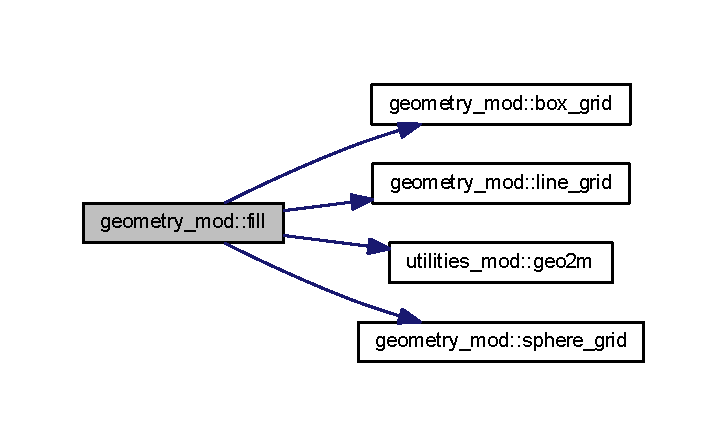
\includegraphics[width=349pt]{namespacegeometry__mod_a1d97564e04562532b5389bfb91aa676b_cgraph}
\end{center}
\end{figure}
\mbox{\Hypertarget{namespacegeometry__mod_ad790edd694561b33dad20cfa3a14e8f2}\label{namespacegeometry__mod_ad790edd694561b33dad20cfa3a14e8f2}} 
\index{geometry\+\_\+mod@{geometry\+\_\+mod}!fillsize@{fillsize}}
\index{fillsize@{fillsize}!geometry\+\_\+mod@{geometry\+\_\+mod}}
\subsubsection{\texorpdfstring{fillsize()}{fillsize()}}
{\footnotesize\ttfamily integer function geometry\+\_\+mod\+::fillsize (\begin{DoxyParamCaption}\item[{class(\mbox{\hyperlink{structgeometry__mod_1_1geometry__class}{geometry\+\_\+class}}), intent(in)}]{self,  }\item[{class(\mbox{\hyperlink{structgeometry__mod_1_1shape}{shape}}), intent(in)}]{shapetype,  }\item[{real(prec), intent(in)}]{dp }\end{DoxyParamCaption})\hspace{0.3cm}{\ttfamily [private]}}



method to get the number of points that fill a given geometry 

\begin{DoxyAuthor}{Author}
Ricardo Birjukovs Canelas -\/ M\+A\+R\+E\+T\+EC 
\end{DoxyAuthor}

\begin{DoxyParams}[1]{Parameters}
\mbox{\tt in}  & {\em self,shapetype,dp} & \\
\hline
\end{DoxyParams}


Definition at line 114 of file geometry.\+f90.


\begin{DoxyCode}
114     \textcolor{keywordtype}{implicit none}
115     \textcolor{keywordtype}{class}(geometry\_class), \textcolor{keywordtype}{intent(in)} :: self
116     \textcolor{keywordtype}{class}(shape), \textcolor{keywordtype}{intent(in)} :: shapetype
117     \textcolor{keywordtype}{real(prec)}, \textcolor{keywordtype}{intent(in)} :: dp
118     \textcolor{keywordtype}{integer} :: fillsize
119     \textcolor{keywordtype}{type}(vector) :: temp
120     \textcolor{keywordtype}{type}(string) :: outext
121     \textcolor{keywordflow}{select type} (shapetype)
122 \textcolor{keywordflow}{    type is} (shape)
123 \textcolor{keywordflow}{    class is} (box)
124         fillsize = max((int(shapetype%size%x/dp)+1)*(int(shapetype%size%y/dp)+1)*(int(shapetype%size%z/dp)+
      1),1)
125 \textcolor{keywordflow}{    class is} (point)
126         fillsize = 1
127 \textcolor{keywordflow}{    class is} (line)
128         temp = shapetype%pt - shapetype%last
129         temp = geo2m(temp, shapetype%pt%y)
130         fillsize = max(int(temp%normL2()/dp),1)
131 \textcolor{keywordflow}{    class is} (sphere)
132         fillsize = sphere\_np\_count(dp, shapetype%radius)
133 \textcolor{keywordflow}{        class default}
134         outext=\textcolor{stringliteral}{'[geometry::fillsize] : unexpected type for geometry object, stoping'}
135         \textcolor{keyword}{call }log%put(outext)
136         stop
137 \textcolor{keywordflow}{    end select}
\end{DoxyCode}
Here is the call graph for this function\+:\nopagebreak
\begin{figure}[H]
\begin{center}
\leavevmode
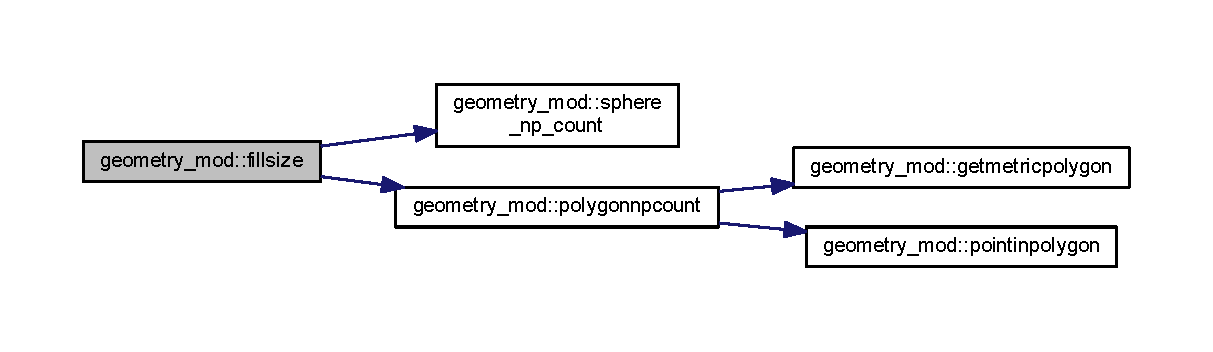
\includegraphics[width=346pt]{namespacegeometry__mod_ad790edd694561b33dad20cfa3a14e8f2_cgraph}
\end{center}
\end{figure}
\mbox{\Hypertarget{namespacegeometry__mod_a4a38edbff02aa0ff5f16a16c39bf778e}\label{namespacegeometry__mod_a4a38edbff02aa0ff5f16a16c39bf778e}} 
\index{geometry\+\_\+mod@{geometry\+\_\+mod}!getcenter@{getcenter}}
\index{getcenter@{getcenter}!geometry\+\_\+mod@{geometry\+\_\+mod}}
\subsubsection{\texorpdfstring{getcenter()}{getcenter()}}
{\footnotesize\ttfamily type(vector) function geometry\+\_\+mod\+::getcenter (\begin{DoxyParamCaption}\item[{class(\mbox{\hyperlink{structgeometry__mod_1_1geometry__class}{geometry\+\_\+class}}), intent(in)}]{self,  }\item[{class(\mbox{\hyperlink{structgeometry__mod_1_1shape}{shape}}), intent(in)}]{shapetype }\end{DoxyParamCaption})\hspace{0.3cm}{\ttfamily [private]}}



method to get the baricenter of a given geometry 

\begin{DoxyAuthor}{Author}
Ricardo Birjukovs Canelas -\/ M\+A\+R\+E\+T\+EC 
\end{DoxyAuthor}

\begin{DoxyParams}[1]{Parameters}
\mbox{\tt in}  & {\em self,shapetype} & \\
\hline
\end{DoxyParams}


Definition at line 179 of file geometry.\+f90.


\begin{DoxyCode}
179     \textcolor{keywordtype}{implicit none}
180     \textcolor{keywordtype}{class}(geometry\_class), \textcolor{keywordtype}{intent(in)} :: self
181     \textcolor{keywordtype}{class}(shape), \textcolor{keywordtype}{intent(in)} :: shapetype
182     \textcolor{keywordtype}{type}(vector) :: center
183     \textcolor{keywordtype}{type}(string) :: outext
184     \textcolor{keywordflow}{select type} (shapetype)
185 \textcolor{keywordflow}{    type is} (shape)
186 \textcolor{keywordflow}{    class is} (box)
187         center = shapetype%pt + m2geo(shapetype%size, shapetype%pt%y)/2.0
188 \textcolor{keywordflow}{    class is} (point)
189         center = shapetype%pt
190 \textcolor{keywordflow}{    class is} (line)
191         center = shapetype%pt + shapetype%last/2.0
192 \textcolor{keywordflow}{    class is} (sphere)
193         center = shapetype%pt
194 \textcolor{keywordflow}{        class default}
195         outext=\textcolor{stringliteral}{'[geometry::getCenter] : unexpected type for geometry object, stoping'}
196         \textcolor{keyword}{call }log%put(outext)
197         stop
198 \textcolor{keywordflow}{    end select}
\end{DoxyCode}
Here is the call graph for this function\+:\nopagebreak
\begin{figure}[H]
\begin{center}
\leavevmode
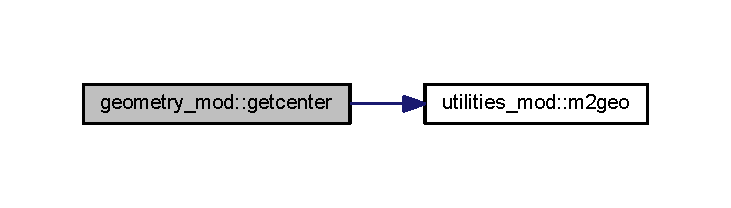
\includegraphics[width=350pt]{namespacegeometry__mod_a4a38edbff02aa0ff5f16a16c39bf778e_cgraph}
\end{center}
\end{figure}
\mbox{\Hypertarget{namespacegeometry__mod_a524c5d28a80fb6729b102126485605ce}\label{namespacegeometry__mod_a524c5d28a80fb6729b102126485605ce}} 
\index{geometry\+\_\+mod@{geometry\+\_\+mod}!getnumpoints@{getnumpoints}}
\index{getnumpoints@{getnumpoints}!geometry\+\_\+mod@{geometry\+\_\+mod}}
\subsubsection{\texorpdfstring{getnumpoints()}{getnumpoints()}}
{\footnotesize\ttfamily integer function geometry\+\_\+mod\+::getnumpoints (\begin{DoxyParamCaption}\item[{class(\mbox{\hyperlink{structgeometry__mod_1_1geometry__class}{geometry\+\_\+class}}), intent(in)}]{self,  }\item[{class(\mbox{\hyperlink{structgeometry__mod_1_1shape}{shape}}), intent(in)}]{shapetype }\end{DoxyParamCaption})\hspace{0.3cm}{\ttfamily [private]}}



method the points defining a given geometry 

\begin{DoxyAuthor}{Author}
Ricardo Birjukovs Canelas -\/ M\+A\+R\+E\+T\+EC 
\end{DoxyAuthor}

\begin{DoxyParams}[1]{Parameters}
\mbox{\tt in}  & {\em self,shapetype} & \\
\hline
\end{DoxyParams}


Definition at line 256 of file geometry.\+f90.


\begin{DoxyCode}
256     \textcolor{keywordtype}{class}(geometry\_class), \textcolor{keywordtype}{intent(in)} :: self
257     \textcolor{keywordtype}{class}(shape), \textcolor{keywordtype}{intent(in)} :: shapetype
258     \textcolor{keywordtype}{integer} :: n
259     \textcolor{keywordtype}{type}(string) :: outext
260     \textcolor{keywordflow}{select type} (shapetype)
261 \textcolor{keywordflow}{    type is} (shape)
262 \textcolor{keywordflow}{    class is} (box)
263         n=8
264 \textcolor{keywordflow}{    class is} (point)
265         n=1
266 \textcolor{keywordflow}{    class is} (line)
267         n=2
268 \textcolor{keywordflow}{    class is} (sphere)
269         n=1
270 \textcolor{keywordflow}{        class default}
271         outext=\textcolor{stringliteral}{'[geometry::getnumPoints] : unexpected type for geometry object, stoping'}
272         \textcolor{keyword}{call }log%put(outext)
273         stop
274 \textcolor{keywordflow}{    end select}
\end{DoxyCode}
\mbox{\Hypertarget{namespacegeometry__mod_a0b1a3c5aa414292ace34d59487082e3a}\label{namespacegeometry__mod_a0b1a3c5aa414292ace34d59487082e3a}} 
\index{geometry\+\_\+mod@{geometry\+\_\+mod}!getpoints@{getpoints}}
\index{getpoints@{getpoints}!geometry\+\_\+mod@{geometry\+\_\+mod}}
\subsubsection{\texorpdfstring{getpoints()}{getpoints()}}
{\footnotesize\ttfamily type(vector) function, dimension(\+:), allocatable geometry\+\_\+mod\+::getpoints (\begin{DoxyParamCaption}\item[{class(\mbox{\hyperlink{structgeometry__mod_1_1geometry__class}{geometry\+\_\+class}}), intent(in)}]{self,  }\item[{class(\mbox{\hyperlink{structgeometry__mod_1_1shape}{shape}}), intent(in)}]{shapetype }\end{DoxyParamCaption})\hspace{0.3cm}{\ttfamily [private]}}



method that returns the points defining a given geometry 

\begin{DoxyAuthor}{Author}
Ricardo Birjukovs Canelas -\/ M\+A\+R\+E\+T\+EC 
\end{DoxyAuthor}

\begin{DoxyParams}[1]{Parameters}
\mbox{\tt in}  & {\em self,shapetype} & \\
\hline
\end{DoxyParams}


Definition at line 208 of file geometry.\+f90.


\begin{DoxyCode}
208     \textcolor{keywordtype}{class}(geometry\_class), \textcolor{keywordtype}{intent(in)} :: self
209     \textcolor{keywordtype}{class}(shape), \textcolor{keywordtype}{intent(in)} :: shapetype
210     \textcolor{keywordtype}{type}(vector), \textcolor{keywordtype}{allocatable} :: pts(:)
211     \textcolor{keywordtype}{type}(string) :: outext
212     \textcolor{keywordtype}{integer} :: n
213     \textcolor{keywordtype}{type}(vector) :: temp
214     \textcolor{keywordflow}{select type} (shapetype)
215 \textcolor{keywordflow}{    type is} (shape)
216 \textcolor{keywordflow}{    class is} (box)
217         n=8
218         \textcolor{keyword}{allocate}(pts(n))
219         temp = shapetype%size
220         \textcolor{comment}{!temp = m2geo(shapetype%size, shapetype%pt%y)}
221         pts(1) = shapetype%pt
222         pts(2) = shapetype%pt + temp%y*ey
223         pts(3) = pts(2) + temp%z*ez
224         pts(4) = shapetype%pt + temp%z*ez
225         pts(5) = shapetype%pt + temp%x*ex
226         pts(6) = pts(5) + temp%y*ey
227         pts(7) = shapetype%pt + temp
228         pts(8) = pts(5) + temp%z*ez
229 \textcolor{keywordflow}{    class is} (point)
230         n=1
231         \textcolor{keyword}{allocate}(pts(n))
232         pts(1) = shapetype%pt
233 \textcolor{keywordflow}{    class is} (line)
234         n=2
235         \textcolor{keyword}{allocate}(pts(n))
236         pts(1) = shapetype%pt
237         pts(2) = shapetype%last
238 \textcolor{keywordflow}{    class is} (sphere)
239         n=1
240         \textcolor{keyword}{allocate}(pts(n))
241         pts(1) = shapetype%pt
242 \textcolor{keywordflow}{        class default}
243         outext=\textcolor{stringliteral}{'[geometry::getPoints] : unexpected type for geometry object, stoping'}
244         \textcolor{keyword}{call }log%put(outext)
245         stop
246 \textcolor{keywordflow}{    end select}
\end{DoxyCode}
\mbox{\Hypertarget{namespacegeometry__mod_a22dd77024fce56da299445a697256155}\label{namespacegeometry__mod_a22dd77024fce56da299445a697256155}} 
\index{geometry\+\_\+mod@{geometry\+\_\+mod}!inlist@{inlist}}
\index{inlist@{inlist}!geometry\+\_\+mod@{geometry\+\_\+mod}}
\subsubsection{\texorpdfstring{inlist()}{inlist()}}
{\footnotesize\ttfamily logical function geometry\+\_\+mod\+::inlist (\begin{DoxyParamCaption}\item[{class(\mbox{\hyperlink{structgeometry__mod_1_1geometry__class}{geometry\+\_\+class}}), intent(in)}]{self,  }\item[{type(string), intent(in)}]{geomname }\end{DoxyParamCaption})\hspace{0.3cm}{\ttfamily [private]}}



Public function that returns a logical if the input geometry name is valid. 

\begin{DoxyAuthor}{Author}
Ricardo Birjukovs Canelas -\/ M\+A\+R\+E\+T\+EC 
\end{DoxyAuthor}

\begin{DoxyParams}[1]{Parameters}
\mbox{\tt in}  & {\em self,geomname} & \\
\hline
\end{DoxyParams}


Definition at line 95 of file geometry.\+f90.


\begin{DoxyCode}
95     \textcolor{keywordtype}{implicit none}
96     \textcolor{keywordtype}{class}(geometry\_class), \textcolor{keywordtype}{intent(in)} :: self
97     \textcolor{keywordtype}{type}(string), \textcolor{keywordtype}{intent(in)} :: geomname
98     \textcolor{keywordtype}{integer} :: i
99     tf = .false.
100     \textcolor{keywordflow}{do} i=1, \textcolor{keyword}{size}(self%list)
101         \textcolor{keywordflow}{if} (geomname == self%list(i)) \textcolor{keywordflow}{then}
102             tf = .true.
103 \textcolor{keywordflow}{        endif}
104 \textcolor{keywordflow}{    enddo}
\end{DoxyCode}
\mbox{\Hypertarget{namespacegeometry__mod_abcb09c0f5274c27cb79b0dd009ed94b3}\label{namespacegeometry__mod_abcb09c0f5274c27cb79b0dd009ed94b3}} 
\index{geometry\+\_\+mod@{geometry\+\_\+mod}!line\+\_\+grid@{line\+\_\+grid}}
\index{line\+\_\+grid@{line\+\_\+grid}!geometry\+\_\+mod@{geometry\+\_\+mod}}
\subsubsection{\texorpdfstring{line\+\_\+grid()}{line\_grid()}}
{\footnotesize\ttfamily subroutine geometry\+\_\+mod\+::line\+\_\+grid (\begin{DoxyParamCaption}\item[{real(prec), intent(in)}]{dp,  }\item[{type(vector), intent(in)}]{dist,  }\item[{integer, intent(in)}]{np,  }\item[{type(vector), dimension(np), intent(out)}]{ptlist }\end{DoxyParamCaption})\hspace{0.3cm}{\ttfamily [private]}}



private routine that returns the points distributed on a grid with spacing dp along a line 

\begin{DoxyAuthor}{Author}
Ricardo Birjukovs Canelas -\/ M\+A\+R\+E\+T\+EC 
\end{DoxyAuthor}

\begin{DoxyParams}[1]{Parameters}
\mbox{\tt in}  & {\em dp,dist,np,ptlist} & \\
\hline
\end{DoxyParams}


Definition at line 425 of file geometry.\+f90.


\begin{DoxyCode}
425     \textcolor{keywordtype}{implicit none}
426     \textcolor{keywordtype}{real(prec)}, \textcolor{keywordtype}{intent(in)} :: dp
427     \textcolor{keywordtype}{type}(vector), \textcolor{keywordtype}{intent(in)} :: dist
428     \textcolor{keywordtype}{integer}, \textcolor{keywordtype}{intent(in)}::  np
429     \textcolor{keywordtype}{type}(vector), \textcolor{keywordtype}{intent(out)} :: ptlist(np)
430     \textcolor{keywordtype}{integer} :: i, j, k, p
431 
432     \textcolor{keywordflow}{do} p=1, np
433         ptlist(p) = dp/np*(dist*(p-1))
434 \textcolor{keywordflow}{    end do}
435     \textcolor{keywordflow}{if} (np == 1) \textcolor{keywordflow}{then} \textcolor{comment}{!Just the origin}
436         ptlist(1)= 0*ex + 0*ey +0*ez
437 \textcolor{keywordflow}{    end if}
\end{DoxyCode}
Here is the caller graph for this function\+:\nopagebreak
\begin{figure}[H]
\begin{center}
\leavevmode
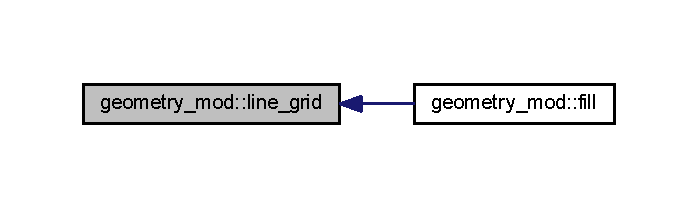
\includegraphics[width=335pt]{namespacegeometry__mod_abcb09c0f5274c27cb79b0dd009ed94b3_icgraph}
\end{center}
\end{figure}
\mbox{\Hypertarget{namespacegeometry__mod_aed4426181ca851b41717edd50268e5f3}\label{namespacegeometry__mod_aed4426181ca851b41717edd50268e5f3}} 
\index{geometry\+\_\+mod@{geometry\+\_\+mod}!printgeometry@{printgeometry}}
\index{printgeometry@{printgeometry}!geometry\+\_\+mod@{geometry\+\_\+mod}}
\subsubsection{\texorpdfstring{printgeometry()}{printgeometry()}}
{\footnotesize\ttfamily subroutine geometry\+\_\+mod\+::printgeometry (\begin{DoxyParamCaption}\item[{class(\mbox{\hyperlink{structgeometry__mod_1_1geometry__class}{geometry\+\_\+class}}), intent(in)}]{self,  }\item[{class(\mbox{\hyperlink{structgeometry__mod_1_1shape}{shape}})}]{shapetype }\end{DoxyParamCaption})\hspace{0.3cm}{\ttfamily [private]}}



method to print the details of a given geometry 

\begin{DoxyAuthor}{Author}
Ricardo Birjukovs Canelas -\/ M\+A\+R\+E\+T\+EC 
\end{DoxyAuthor}

\begin{DoxyParams}[1]{Parameters}
\mbox{\tt in}  & {\em self,shapetype} & \\
\hline
\end{DoxyParams}


Definition at line 284 of file geometry.\+f90.


\begin{DoxyCode}
284     \textcolor{keywordtype}{implicit none}
285     \textcolor{keywordtype}{class}(geometry\_class), \textcolor{keywordtype}{intent(in)} :: self
286     \textcolor{keywordtype}{class}(shape) :: shapetype
287 
288     \textcolor{keywordtype}{type}(vector) :: temp(2)
289     \textcolor{keywordtype}{type}(string) :: temp\_str(6)
290     \textcolor{keywordtype}{type}(string) :: outext
291 
292     temp\_str(1) = shapetype%pt%x
293     temp\_str(2) = shapetype%pt%y
294     temp\_str(3) = shapetype%pt%z
295     \textcolor{keywordflow}{select type} (shapetype)
296 \textcolor{keywordflow}{    type is} (shape)
297 \textcolor{keywordflow}{    class is} (box)
298         temp\_str(4) = shapetype%size%x
299         temp\_str(5) = shapetype%size%y
300         temp\_str(6) = shapetype%size%z
301         outext=\textcolor{stringliteral}{'      Box at '}//temp\_str(1)//\textcolor{stringliteral}{' '}//temp\_str(2)//\textcolor{stringliteral}{' '}//temp\_str(3)//new\_line(\textcolor{stringliteral}{'a'})//&
302             \textcolor{stringliteral}{'       with '}//temp\_str(4)//\textcolor{stringliteral}{' X '}//temp\_str(5)//\textcolor{stringliteral}{' X '}//temp\_str(6)
303 \textcolor{keywordflow}{    class is} (point)
304         outext=\textcolor{stringliteral}{'      Point at '}//temp\_str(1)//\textcolor{stringliteral}{' '}//temp\_str(2)//\textcolor{stringliteral}{' '}//temp\_str(3)
305 \textcolor{keywordflow}{    class is} (line)
306         temp\_str(4) = shapetype%last%x
307         temp\_str(5) = shapetype%last%y
308         temp\_str(6) = shapetype%last%z
309         outext=\textcolor{stringliteral}{'      Line from '}//temp\_str(1)//\textcolor{stringliteral}{' '}//temp\_str(2)//\textcolor{stringliteral}{' '}//temp\_str(3)//new\_line(\textcolor{stringliteral}{'a'})//&
310             \textcolor{stringliteral}{'       to '}//temp\_str(4)//\textcolor{stringliteral}{' X '}//temp\_str(5)//\textcolor{stringliteral}{' X '}//temp\_str(6)
311 \textcolor{keywordflow}{    class is} (sphere)
312         temp\_str(4) = shapetype%radius
313         outext=\textcolor{stringliteral}{'      Sphere at '}//temp\_str(1)//\textcolor{stringliteral}{' '}//temp\_str(2)//\textcolor{stringliteral}{' '}//temp\_str(3)//new\_line(\textcolor{stringliteral}{'a'})//&
314             \textcolor{stringliteral}{'       with radius '}//temp\_str(4)
315 \textcolor{keywordflow}{        class default}
316         outext=\textcolor{stringliteral}{'[geometry::print] : unexpected type for geometry object, stoping'}
317         \textcolor{keyword}{call }log%put(outext)
318         stop
319 \textcolor{keywordflow}{    end select}
320     \textcolor{keyword}{call }log%put(outext,.false.)
321 
\end{DoxyCode}
\mbox{\Hypertarget{namespacegeometry__mod_a6c03a4ea3de6763940396dbeb3908ebc}\label{namespacegeometry__mod_a6c03a4ea3de6763940396dbeb3908ebc}} 
\index{geometry\+\_\+mod@{geometry\+\_\+mod}!sphere\+\_\+grid@{sphere\+\_\+grid}}
\index{sphere\+\_\+grid@{sphere\+\_\+grid}!geometry\+\_\+mod@{geometry\+\_\+mod}}
\subsubsection{\texorpdfstring{sphere\+\_\+grid()}{sphere\_grid()}}
{\footnotesize\ttfamily subroutine geometry\+\_\+mod\+::sphere\+\_\+grid (\begin{DoxyParamCaption}\item[{real(prec), intent(in)}]{dp,  }\item[{real(prec), intent(in)}]{r,  }\item[{integer, intent(in)}]{np,  }\item[{type(vector), dimension(np), intent(out)}]{ptlist }\end{DoxyParamCaption})\hspace{0.3cm}{\ttfamily [private]}}



private routine that returns the points distributed on a grid with spacing dp inside a sphere 

\begin{DoxyAuthor}{Author}
Ricardo Birjukovs Canelas -\/ M\+A\+R\+E\+T\+EC 
\end{DoxyAuthor}

\begin{DoxyParams}[1]{Parameters}
\mbox{\tt in}  & {\em dp,r,np,ptlist} & \\
\hline
\end{DoxyParams}


Definition at line 363 of file geometry.\+f90.


\begin{DoxyCode}
363     \textcolor{keywordtype}{implicit none}
364     \textcolor{keywordtype}{real(prec)}, \textcolor{keywordtype}{intent(in)} :: dp
365     \textcolor{keywordtype}{real(prec)}, \textcolor{keywordtype}{intent(in)} :: r
366     \textcolor{keywordtype}{integer}, \textcolor{keywordtype}{intent(in)}::  np
367     \textcolor{keywordtype}{type}(vector), \textcolor{keywordtype}{intent(out)} :: ptlist(np)
368     \textcolor{keywordtype}{integer} :: i, j, k, p, n
369     \textcolor{keywordtype}{type}(vector) :: pts
370     n=int(3*r/dp)
371     p=0
372     \textcolor{keywordflow}{do} i=1, n
373         \textcolor{keywordflow}{do} j=1, n
374             \textcolor{keywordflow}{do} k=1, n
375                 pts = dp*(ex*(i-1)+ey*(j-1)+ez*(k-1)) - r*(ex+ey+ez)
376                 \textcolor{keywordflow}{if} (pts%normL2() .le. r) \textcolor{keywordflow}{then}
377                     p=p+1
378                     ptlist(p)=pts
379 \textcolor{keywordflow}{                end if}
380 \textcolor{keywordflow}{            end do}
381 \textcolor{keywordflow}{        end do}
382 \textcolor{keywordflow}{    end do}
383     \textcolor{keywordflow}{if} (np == 1) \textcolor{keywordflow}{then} \textcolor{comment}{!Just the center point}
384         ptlist(1)= 0*ex + 0*ey +0*ez
385 \textcolor{keywordflow}{    end if}
386 
\end{DoxyCode}
Here is the caller graph for this function\+:\nopagebreak
\begin{figure}[H]
\begin{center}
\leavevmode
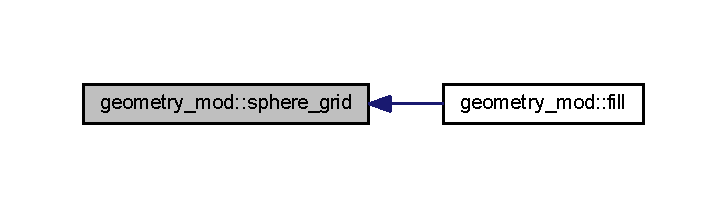
\includegraphics[width=349pt]{namespacegeometry__mod_a6c03a4ea3de6763940396dbeb3908ebc_icgraph}
\end{center}
\end{figure}
\mbox{\Hypertarget{namespacegeometry__mod_a05de7940b4e7df5a2b31f3d0414e3743}\label{namespacegeometry__mod_a05de7940b4e7df5a2b31f3d0414e3743}} 
\index{geometry\+\_\+mod@{geometry\+\_\+mod}!sphere\+\_\+np\+\_\+count@{sphere\+\_\+np\+\_\+count}}
\index{sphere\+\_\+np\+\_\+count@{sphere\+\_\+np\+\_\+count}!geometry\+\_\+mod@{geometry\+\_\+mod}}
\subsubsection{\texorpdfstring{sphere\+\_\+np\+\_\+count()}{sphere\_np\_count()}}
{\footnotesize\ttfamily integer function geometry\+\_\+mod\+::sphere\+\_\+np\+\_\+count (\begin{DoxyParamCaption}\item[{real(prec), intent(in)}]{dp,  }\item[{real(prec), intent(in)}]{r }\end{DoxyParamCaption})\hspace{0.3cm}{\ttfamily [private]}}



private function that returns the number of points distributed on a grid with spacing dp inside a sphere 

\begin{DoxyAuthor}{Author}
Ricardo Birjukovs Canelas -\/ M\+A\+R\+E\+T\+EC 
\end{DoxyAuthor}

\begin{DoxyParams}[1]{Parameters}
\mbox{\tt in}  & {\em dp,r} & \\
\hline
\end{DoxyParams}


Definition at line 332 of file geometry.\+f90.


\begin{DoxyCode}
332     \textcolor{keywordtype}{implicit none}
333     \textcolor{keywordtype}{real(prec)}, \textcolor{keywordtype}{intent(in)} :: dp
334     \textcolor{keywordtype}{real(prec)}, \textcolor{keywordtype}{intent(in)} :: r
335     \textcolor{keywordtype}{integer} :: np
336     \textcolor{keywordtype}{integer} :: i, j, k, n
337     \textcolor{keywordtype}{type}(vector) :: pts
338     np=0
339     n=int(3*r/dp)
340     \textcolor{keywordflow}{do} i=1, n
341         \textcolor{keywordflow}{do} j=1, n
342             \textcolor{keywordflow}{do} k=1, n
343                 pts = dp*(ex*(i-1)+ey*(j-1)+ez*(k-1)) - r*(ex+ey+ez)
344                 \textcolor{keywordflow}{if} (pts%normL2() .le. r) \textcolor{keywordflow}{then}
345                     np=np+1
346 \textcolor{keywordflow}{                end if}
347 \textcolor{keywordflow}{            end do}
348 \textcolor{keywordflow}{        end do}
349 \textcolor{keywordflow}{    end do}
350     \textcolor{keywordflow}{if} (np == 0) \textcolor{keywordflow}{then} \textcolor{comment}{!Just the center point}
351         np=1
352 \textcolor{keywordflow}{    end if}
\end{DoxyCode}
Here is the caller graph for this function\+:\nopagebreak
\begin{figure}[H]
\begin{center}
\leavevmode
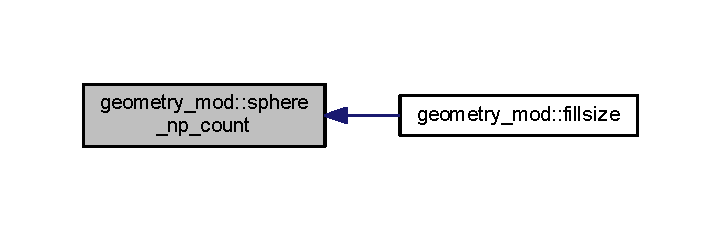
\includegraphics[width=346pt]{namespacegeometry__mod_a05de7940b4e7df5a2b31f3d0414e3743_icgraph}
\end{center}
\end{figure}


\subsection{Variable Documentation}
\mbox{\Hypertarget{namespacegeometry__mod_ad2ad4f7e1138beaad5f37d5c15b7b457}\label{namespacegeometry__mod_ad2ad4f7e1138beaad5f37d5c15b7b457}} 
\index{geometry\+\_\+mod@{geometry\+\_\+mod}!geometry@{geometry}}
\index{geometry@{geometry}!geometry\+\_\+mod@{geometry\+\_\+mod}}
\subsubsection{\texorpdfstring{geometry}{geometry}}
{\footnotesize\ttfamily type(\mbox{\hyperlink{structgeometry__mod_1_1geometry__class}{geometry\+\_\+class}}), public geometry\+\_\+mod\+::geometry}



Definition at line 65 of file geometry.\+f90.


\begin{DoxyCode}
65     \textcolor{keywordtype}{type}(geometry\_class) :: Geometry
\end{DoxyCode}

\hypertarget{namespacehdf5parser__mod}{}\section{hdf5parser\+\_\+mod Module Reference}
\label{namespacehdf5parser__mod}\index{hdf5parser\+\_\+mod@{hdf5parser\+\_\+mod}}


Module that defines a hdf5 file model class, responsible for abstracting the parsing of hdf5 M\+O\+H\+ID files. Each object of this class is responsible for one file, effectivelly representing it. The object should return the necessary data fields with corresponding meta data, such as names and units.  


\subsection*{Data Types}
\begin{DoxyCompactItemize}
\item 
type \mbox{\hyperlink{structhdf5parser__mod_1_1dim__t}{dim\+\_\+t}}
\item 
type \mbox{\hyperlink{structhdf5parser__mod_1_1hdf5file__class}{hdf5file\+\_\+class}}
\begin{DoxyCompactList}\small\item\em A class that models a hdf5 mohid file. \end{DoxyCompactList}\item 
type \mbox{\hyperlink{structhdf5parser__mod_1_1var__t}{var\+\_\+t}}
\end{DoxyCompactItemize}


\subsection{Detailed Description}
Module that defines a hdf5 file model class, responsible for abstracting the parsing of hdf5 M\+O\+H\+ID files. Each object of this class is responsible for one file, effectivelly representing it. The object should return the necessary data fields with corresponding meta data, such as names and units. 

\begin{DoxyAuthor}{Author}
Ricardo Birjukovs Canelas 
\end{DoxyAuthor}

\hypertarget{namespacehdf5writter__mod}{}\section{hdf5writter\+\_\+mod Module Reference}
\label{namespacehdf5writter__mod}\index{hdf5writter\+\_\+mod@{hdf5writter\+\_\+mod}}


Defines a vtk writer class with an object exposable to the Output streamer. Writes files in .xml vtk, both in serial and parallel model. Uses an unstructured mesh format specifier to store any type of data, both meshes and Tracers. Supports scalar and vectorial data.  


\subsection*{Data Types}
\begin{DoxyCompactItemize}
\item 
type \mbox{\hyperlink{structhdf5writter__mod_1_1hdf5writter__class}{hdf5writter\+\_\+class}}
\end{DoxyCompactItemize}
\subsection*{Functions/\+Subroutines}
\begin{DoxyCompactItemize}
\item 
subroutine \mbox{\hyperlink{namespacehdf5writter__mod_a2409af91a67db06badcb9ae439142f92}{inithdf5writter}} (self)
\begin{DoxyCompactList}\small\item\em Initializes a H\+D\+F5 writer object. \end{DoxyCompactList}\item 
subroutine \mbox{\hyperlink{namespacehdf5writter__mod_a0318c234490ab15f480e7f940266ec4f}{closehdf5writer}} (self)
\begin{DoxyCompactList}\small\item\em Closes a H\+D\+F5 writer object. \end{DoxyCompactList}\item 
subroutine \mbox{\hyperlink{namespacehdf5writter__mod_a5f79038dbb067a692a12d171e51b5703}{tracerserial}} (self, filename, blocks)
\begin{DoxyCompactList}\small\item\em Public Tracer writting routine. Writes Tracer data in M\+O\+H\+ID H\+D\+F5 format. \end{DoxyCompactList}\item 
subroutine \mbox{\hyperlink{namespacehdf5writter__mod_adc4cbad9398ee6e9cb5723a30a7c44b1}{writetestmatrix}} (mat)
\end{DoxyCompactItemize}


\subsection{Detailed Description}
Defines a vtk writer class with an object exposable to the Output streamer. Writes files in .xml vtk, both in serial and parallel model. Uses an unstructured mesh format specifier to store any type of data, both meshes and Tracers. Supports scalar and vectorial data. 

\begin{DoxyAuthor}{Author}
Ricardo Birjukovs Canelas 
\end{DoxyAuthor}


\subsection{Function/\+Subroutine Documentation}
\mbox{\Hypertarget{namespacehdf5writter__mod_a0318c234490ab15f480e7f940266ec4f}\label{namespacehdf5writter__mod_a0318c234490ab15f480e7f940266ec4f}} 
\index{hdf5writter\+\_\+mod@{hdf5writter\+\_\+mod}!closehdf5writer@{closehdf5writer}}
\index{closehdf5writer@{closehdf5writer}!hdf5writter\+\_\+mod@{hdf5writter\+\_\+mod}}
\subsubsection{\texorpdfstring{closehdf5writer()}{closehdf5writer()}}
{\footnotesize\ttfamily subroutine hdf5writter\+\_\+mod\+::closehdf5writer (\begin{DoxyParamCaption}\item[{class(\mbox{\hyperlink{structhdf5writter__mod_1_1hdf5writter__class}{hdf5writter\+\_\+class}}), intent(inout)}]{self }\end{DoxyParamCaption})\hspace{0.3cm}{\ttfamily [private]}}



Closes a H\+D\+F5 writer object. 

\begin{DoxyAuthor}{Author}
Ricardo Birjukovs Canelas -\/ M\+A\+R\+E\+T\+EC 
\end{DoxyAuthor}


Definition at line 63 of file H\+D\+F5writter.\+f90.


\begin{DoxyCode}
63     \textcolor{keywordtype}{class}(hdf5writter\_class), \textcolor{keywordtype}{intent(inout)} :: self
64 
\end{DoxyCode}
\mbox{\Hypertarget{namespacehdf5writter__mod_a2409af91a67db06badcb9ae439142f92}\label{namespacehdf5writter__mod_a2409af91a67db06badcb9ae439142f92}} 
\index{hdf5writter\+\_\+mod@{hdf5writter\+\_\+mod}!inithdf5writter@{inithdf5writter}}
\index{inithdf5writter@{inithdf5writter}!hdf5writter\+\_\+mod@{hdf5writter\+\_\+mod}}
\subsubsection{\texorpdfstring{inithdf5writter()}{inithdf5writter()}}
{\footnotesize\ttfamily subroutine hdf5writter\+\_\+mod\+::inithdf5writter (\begin{DoxyParamCaption}\item[{class(\mbox{\hyperlink{structhdf5writter__mod_1_1hdf5writter__class}{hdf5writter\+\_\+class}}), intent(inout)}]{self }\end{DoxyParamCaption})\hspace{0.3cm}{\ttfamily [private]}}



Initializes a H\+D\+F5 writer object. 

\begin{DoxyAuthor}{Author}
Ricardo Birjukovs Canelas -\/ M\+A\+R\+E\+T\+EC 
\end{DoxyAuthor}


Definition at line 53 of file H\+D\+F5writter.\+f90.


\begin{DoxyCode}
53     \textcolor{keywordtype}{class}(hdf5writter\_class), \textcolor{keywordtype}{intent(inout)} :: self
54     self%numHdf5Files = 0
\end{DoxyCode}
\mbox{\Hypertarget{namespacehdf5writter__mod_a5f79038dbb067a692a12d171e51b5703}\label{namespacehdf5writter__mod_a5f79038dbb067a692a12d171e51b5703}} 
\index{hdf5writter\+\_\+mod@{hdf5writter\+\_\+mod}!tracerserial@{tracerserial}}
\index{tracerserial@{tracerserial}!hdf5writter\+\_\+mod@{hdf5writter\+\_\+mod}}
\subsubsection{\texorpdfstring{tracerserial()}{tracerserial()}}
{\footnotesize\ttfamily subroutine hdf5writter\+\_\+mod\+::tracerserial (\begin{DoxyParamCaption}\item[{class(\mbox{\hyperlink{structhdf5writter__mod_1_1hdf5writter__class}{hdf5writter\+\_\+class}}), intent(inout)}]{self,  }\item[{type(string), intent(in)}]{filename,  }\item[{class(\mbox{\hyperlink{structblocks__mod_1_1block__class}{block\+\_\+class}}), dimension(\+:), intent(in)}]{blocks }\end{DoxyParamCaption})\hspace{0.3cm}{\ttfamily [private]}}



Public Tracer writting routine. Writes Tracer data in M\+O\+H\+ID H\+D\+F5 format. 

\begin{DoxyAuthor}{Author}
Ricardo Birjukovs Canelas -\/ M\+A\+R\+E\+T\+EC 
\end{DoxyAuthor}

\begin{DoxyParams}[1]{Parameters}
\mbox{\tt in}  & {\em self,filename,blocks} & \\
\hline
\mbox{\tt in}  & {\em blocks} & Case Blocks \\
\hline
\end{DoxyParams}


Definition at line 74 of file H\+D\+F5writter.\+f90.


\begin{DoxyCode}
74     \textcolor{keywordtype}{class}(hdf5writter\_class), \textcolor{keywordtype}{intent(inout)} :: self
75     \textcolor{keywordtype}{type}(string), \textcolor{keywordtype}{intent(in)} :: filename
76     \textcolor{keywordtype}{class}(block\_class), \textcolor{keywordtype}{dimension(:)}, \textcolor{keywordtype}{intent(in)} :: blocks
77 
78     \textcolor{keywordtype}{type}(string) :: fullfilename, extfilename
79     \textcolor{keywordtype}{type}(string) :: outext
80     \textcolor{keywordtype}{integer} :: error, i, j, b
81     \textcolor{keywordtype}{integer} :: HDF5\_CREATE, STAT\_CALL
82     \textcolor{keywordtype}{integer}, \textcolor{keywordtype}{pointer} :: ID => null()
83     \textcolor{keywordtype}{integer}, \textcolor{keywordtype}{target} :: id\_target
84     \textcolor{keywordtype}{integer} :: np
85     \textcolor{keywordtype}{logical}, \textcolor{keywordtype}{allocatable}, \textcolor{keywordtype}{dimension(:)} :: active
86 
87     \textcolor{keywordtype}{real}, \textcolor{keywordtype}{dimension(:,:)}, \textcolor{keywordtype}{pointer} :: mat
88     \textcolor{keywordtype}{real}, \textcolor{keywordtype}{dimension(:,:)}, \textcolor{keywordtype}{allocatable}, \textcolor{keywordtype}{target} :: matReal
89     \textcolor{keywordtype}{integer}, \textcolor{keywordtype}{dimension(:,:)}, \textcolor{keywordtype}{pointer} :: matInt
90     \textcolor{keywordtype}{integer}, \textcolor{keywordtype}{dimension(:,:)}, \textcolor{keywordtype}{allocatable}, \textcolor{keywordtype}{target} :: matIntTarget
91     
92     extfilename = filename%chars()//\textcolor{stringliteral}{'.hdf5'}
93     fullfilename = globals%Names%outpath//\textcolor{stringliteral}{'/'}//extfilename
94         
95     \textcolor{comment}{!allocate(mat, source = real(blocks(1)%BlockState(1)%state))}
96     \textcolor{comment}{!allocate(mat(size(blocks(1)%BlockState(1)%state,1), size(blocks(1)%BlockState(1)%state,2)))}
97     \textcolor{comment}{!mat = real(blocks(1)%BlockState(1)%state)}
98     \textcolor{keyword}{allocate}(matreal(\textcolor{keyword}{size}(blocks(1)%BlockState(1)%state,1), \textcolor{keyword}{size}(blocks(1)%BlockState(1)%state,2)))
99     matreal = \textcolor{keywordtype}{real}(blocks(1)%BlockState(1)%state)
100     \textcolor{comment}{!mat => matReal}
101     
102     \textcolor{keyword}{allocate}(mat(\textcolor{keyword}{size}(blocks(1)%BlockState(1)%state,1), \textcolor{keyword}{size}(blocks(1)%BlockState(1)%state,2)))
103     mat => matreal
104     
105     \textcolor{comment}{!allocate(matInt(10,20))}
106     \textcolor{comment}{!matInt = 12}
107     \textcolor{comment}{!call writeTestmatrix(matInt)}
108     
109     \textcolor{keyword}{allocate}(matinttarget(10,20))
110     matinttarget = 12
111     \textcolor{keyword}{allocate}(matint(10,20))
112     matint = matinttarget
113     
114     print*, \textcolor{stringliteral}{'got here'}
115     
116     \textcolor{comment}{!Gets File Access Code}
117     \textcolor{keyword}{call }gethdf5fileaccess(hdf5\_create = hdf5\_create)
118     
119     print*, \textcolor{stringliteral}{'got here'}
120     
121     \textcolor{comment}{!Opens HDF File}
122     \textcolor{comment}{!id\_target = 0}
123     \textcolor{comment}{!ID => id\_target}
124     \textcolor{keyword}{allocate}(id)
125     id = 0
126     \textcolor{keyword}{call }constructhdf5(id, fullfilename%chars(), hdf5\_create, stat = stat\_call)
127     \textcolor{keywordflow}{if} (stat\_call /= success\_) \textcolor{keywordflow}{then}
128         outext = \textcolor{stringliteral}{'[HDF5Writter::TracerSerial]: unnable to create '}//fullfilename//\textcolor{stringliteral}{' file, stoping'}
129         \textcolor{keyword}{call }log%put(outext)
130         stop
131 \textcolor{keywordflow}{    end if}
132     
133     print*, \textcolor{stringliteral}{'got here'}
134     
135     \textcolor{comment}{!writting data}
136     \textcolor{keyword}{call }hdf5writedata(id, \textcolor{stringliteral}{"/Data"}, \textcolor{stringliteral}{"TestMatrix"}, \textcolor{stringliteral}{"-"}, array2d = matint, stat = stat\_call)
137     \textcolor{keywordflow}{if} (stat\_call /= success\_) \textcolor{keywordflow}{then}
138         outext = \textcolor{stringliteral}{'[HDF5Writter::TracerSerial]: unnable to write to '}//fullfilename//\textcolor{stringliteral}{' file, stoping'}
139         \textcolor{keyword}{call }log%put(outext)
140         stop
141 \textcolor{keywordflow}{    end if}
142     
143     \textcolor{keyword}{call }hdf5flushmemory (id, errormessage = \textcolor{stringliteral}{'[HDF5Writter::TracerSerial]: unnable to flush HDF5 writter
       memory'}, stat = stat\_call)
144     \textcolor{keywordflow}{if} (stat\_call /= success\_) \textcolor{keywordflow}{then}
145         outext = \textcolor{stringliteral}{'[HDF5Writter::TracerSerial]: unnable to flush HDF5 writter memory, stoping'}
146         \textcolor{keyword}{call }log%put(outext)
147         stop
148 \textcolor{keywordflow}{    end if}
149 
150     self%numHdf5Files = self%numHdf5Files + 1
151 
\end{DoxyCode}
\mbox{\Hypertarget{namespacehdf5writter__mod_adc4cbad9398ee6e9cb5723a30a7c44b1}\label{namespacehdf5writter__mod_adc4cbad9398ee6e9cb5723a30a7c44b1}} 
\index{hdf5writter\+\_\+mod@{hdf5writter\+\_\+mod}!writetestmatrix@{writetestmatrix}}
\index{writetestmatrix@{writetestmatrix}!hdf5writter\+\_\+mod@{hdf5writter\+\_\+mod}}
\subsubsection{\texorpdfstring{writetestmatrix()}{writetestmatrix()}}
{\footnotesize\ttfamily subroutine hdf5writter\+\_\+mod\+::writetestmatrix (\begin{DoxyParamCaption}\item[{integer, dimension(\+:, \+:), intent(in), pointer}]{mat }\end{DoxyParamCaption})\hspace{0.3cm}{\ttfamily [private]}}



Definition at line 156 of file H\+D\+F5writter.\+f90.


\begin{DoxyCode}
156     \textcolor{keywordtype}{integer}, \textcolor{keywordtype}{dimension(:, :)}, \textcolor{keywordtype}{pointer}, \textcolor{keywordtype}{intent(in)} :: mat
157     \textcolor{keywordtype}{integer} :: ID, HDF5\_CREATE, STAT\_CALL
158 
159     id = 0
160 
161     \textcolor{comment}{!Gets File Access Code}
162     \textcolor{keyword}{call }gethdf5fileaccess(hdf5\_create = hdf5\_create)
163 
164     \textcolor{comment}{!Opens HDF File}
165     \textcolor{keyword}{call }constructhdf5(id, \textcolor{stringliteral}{"filehdf"}, hdf5\_create, stat = stat\_call)
166     \textcolor{keywordflow}{if} (stat\_call /= success\_) stop \textcolor{stringliteral}{'writeTestmatrix - module hdf5Writter\_mod - ERR01'}
167 
168     \textcolor{keyword}{call }hdf5writedata(id, \textcolor{stringliteral}{"/Data"}, \textcolor{stringliteral}{"TestMatrix"}, \textcolor{stringliteral}{"-"},         &
169         array2d = mat,            &
170         stat = stat\_call)
171     \textcolor{keywordflow}{if} (stat\_call /= success\_) stop \textcolor{stringliteral}{'writeTestmatrix - module hdf5Writter\_mod - ERR02'}
172 
173     \textcolor{keyword}{call }hdf5flushmemory (id, errormessage = \textcolor{stringliteral}{'writeTestmatrix - module hdf5Writter\_mod - ERR03'}, stat = 
      stat\_call)
174     \textcolor{keywordflow}{if} (stat\_call /= success\_) stop \textcolor{stringliteral}{'writeTestmatrix - module hdf5Writter\_mod - ERR03'}
175 
\end{DoxyCode}

\hypertarget{namespaceinterpolator__mod}{}\section{interpolator\+\_\+mod Module Reference}
\label{namespaceinterpolator__mod}\index{interpolator\+\_\+mod@{interpolator\+\_\+mod}}


Defines an Interpolator class.  


\subsection*{Data Types}
\begin{DoxyCompactItemize}
\item 
type \mbox{\hyperlink{structinterpolator__mod_1_1interpolator__class}{interpolator\+\_\+class}}
\end{DoxyCompactItemize}
\subsection*{Functions/\+Subroutines}
\begin{DoxyCompactItemize}
\item 
subroutine \mbox{\hyperlink{namespaceinterpolator__mod_ab4d61e34f8feebf8c75e988a6c7cac85}{run}} (self, aot, bdata, time, var\+\_\+dt)
\begin{DoxyCompactList}\small\item\em Method that runs the chosen interpolator method on the given data. \end{DoxyCompactList}\item 
subroutine \mbox{\hyperlink{namespaceinterpolator__mod_a1bf15b6fa6e4fd0bb4a8e544994c487d}{interp4d}} (self, x, y, z, t, field, f\+\_\+out, n\+\_\+fv, n\+\_\+cv, n\+\_\+pv, n\+\_\+tv, n\+\_\+e)
\begin{DoxyCompactList}\small\item\em method to interpolate a particle position in a given data box based on array coordinates. 4d interpolation is a weighted average of 16 neighbors. Consider the 4D domain between the 16 neighbors. The hypercube is divided into 16 sub-\/hypercubes by the point in question. The weight of each neighbor is given by the volume of the opposite sub-\/hypercube, as a fraction of the whole hypercube. \end{DoxyCompactList}\item 
subroutine \mbox{\hyperlink{namespaceinterpolator__mod_adcaf3bba800f19991ed4f33c968184e9}{initinterpolator}} (self, flag, name)
\begin{DoxyCompactList}\small\item\em Initializer method for the Interpolator class. Sets the type of interpolator and name of the algorithm this Interpolator will call. \end{DoxyCompactList}\item 
subroutine \mbox{\hyperlink{namespaceinterpolator__mod_a9b149bc8a3da5d1864b8c049f8b00697}{printinterpolator}} (self)
\begin{DoxyCompactList}\small\item\em Method that prints the Interpolator information. \end{DoxyCompactList}\end{DoxyCompactItemize}


\subsection{Detailed Description}
Defines an Interpolator class. 

\begin{DoxyAuthor}{Author}
Ricardo Birjukovs Canelas 
\end{DoxyAuthor}


\subsection{Function/\+Subroutine Documentation}
\mbox{\Hypertarget{namespaceinterpolator__mod_adcaf3bba800f19991ed4f33c968184e9}\label{namespaceinterpolator__mod_adcaf3bba800f19991ed4f33c968184e9}} 
\index{interpolator\+\_\+mod@{interpolator\+\_\+mod}!initinterpolator@{initinterpolator}}
\index{initinterpolator@{initinterpolator}!interpolator\+\_\+mod@{interpolator\+\_\+mod}}
\subsubsection{\texorpdfstring{initinterpolator()}{initinterpolator()}}
{\footnotesize\ttfamily subroutine interpolator\+\_\+mod\+::initinterpolator (\begin{DoxyParamCaption}\item[{class(\mbox{\hyperlink{structinterpolator__mod_1_1interpolator__class}{interpolator\+\_\+class}}), intent(inout)}]{self,  }\item[{integer, intent(in)}]{flag,  }\item[{type(string), intent(in)}]{name }\end{DoxyParamCaption})\hspace{0.3cm}{\ttfamily [private]}}



Initializer method for the Interpolator class. Sets the type of interpolator and name of the algorithm this Interpolator will call. 

\begin{DoxyAuthor}{Author}
Ricardo Birjukovs Canelas -\/ M\+A\+R\+E\+T\+EC 
\end{DoxyAuthor}

\begin{DoxyParams}[1]{Parameters}
\mbox{\tt in}  & {\em self,flag,name} & \\
\hline
\end{DoxyParams}


Definition at line 172 of file interpolator.\+f90.


\begin{DoxyCode}
172     \textcolor{keywordtype}{class}(interpolator\_class), \textcolor{keywordtype}{intent(inout)} :: self
173     \textcolor{keywordtype}{integer}, \textcolor{keywordtype}{intent(in)} :: flag
174     \textcolor{keywordtype}{type}(string), \textcolor{keywordtype}{intent(in)} :: name
175     self%interpType = flag
176     self%name = name
\end{DoxyCode}
\mbox{\Hypertarget{namespaceinterpolator__mod_a1bf15b6fa6e4fd0bb4a8e544994c487d}\label{namespaceinterpolator__mod_a1bf15b6fa6e4fd0bb4a8e544994c487d}} 
\index{interpolator\+\_\+mod@{interpolator\+\_\+mod}!interp4d@{interp4d}}
\index{interp4d@{interp4d}!interpolator\+\_\+mod@{interpolator\+\_\+mod}}
\subsubsection{\texorpdfstring{interp4d()}{interp4d()}}
{\footnotesize\ttfamily subroutine interpolator\+\_\+mod\+::interp4d (\begin{DoxyParamCaption}\item[{class(\mbox{\hyperlink{structinterpolator__mod_1_1interpolator__class}{interpolator\+\_\+class}}), intent(in)}]{self,  }\item[{real(prec), dimension(n\+\_\+e), intent(in)}]{x,  }\item[{real(prec), dimension(n\+\_\+e), intent(in)}]{y,  }\item[{real(prec), dimension(n\+\_\+e), intent(in)}]{z,  }\item[{real(prec\+\_\+time), intent(in)}]{t,  }\item[{real(prec), dimension(n\+\_\+fv, n\+\_\+cv, n\+\_\+pv, n\+\_\+tv), intent(in)}]{field,  }\item[{real(prec), dimension(n\+\_\+e), intent(out)}]{f\+\_\+out,  }\item[{integer, intent(in)}]{n\+\_\+fv,  }\item[{integer, intent(in)}]{n\+\_\+cv,  }\item[{integer, intent(in)}]{n\+\_\+pv,  }\item[{integer, intent(in)}]{n\+\_\+tv,  }\item[{integer, intent(in)}]{n\+\_\+e }\end{DoxyParamCaption})\hspace{0.3cm}{\ttfamily [private]}}



method to interpolate a particle position in a given data box based on array coordinates. 4d interpolation is a weighted average of 16 neighbors. Consider the 4D domain between the 16 neighbors. The hypercube is divided into 16 sub-\/hypercubes by the point in question. The weight of each neighbor is given by the volume of the opposite sub-\/hypercube, as a fraction of the whole hypercube. 

\begin{DoxyAuthor}{Author}
Daniel Garaboa Paz -\/ U\+SC 
\end{DoxyAuthor}

\begin{DoxyParams}[1]{Parameters}
\mbox{\tt in}  & {\em x,y,z,t,field,n\+\_\+e,f\+\_\+out} & \\
\hline
\mbox{\tt in}  & {\em z} & 1-\/d. Array of particle component positions\\
\hline
\mbox{\tt in}  & {\em t} & time to interpolate to\\
\hline
\mbox{\tt in}  & {\em field} & Field data with dimensions \mbox{[}n\+\_\+fv,n\+\_\+cv,n\+\_\+pv,n\+\_\+tv\mbox{]}\\
\hline
\mbox{\tt out}  & {\em f\+\_\+out} & Field evaluated at x,y,z,t\\
\hline
\mbox{\tt in}  & {\em n\+\_\+tv} & field dimensions\\
\hline
\mbox{\tt in}  & {\em n\+\_\+e} & Number of particles to interpolate to \\
\hline
\end{DoxyParams}


Definition at line 100 of file interpolator.\+f90.


\begin{DoxyCode}
100     \textcolor{keywordtype}{class}(interpolator\_class), \textcolor{keywordtype}{intent(in)} :: self
101     \textcolor{keywordtype}{real(prec)}, \textcolor{keywordtype}{dimension(n\_e)},\textcolor{keywordtype}{intent(in)}:: x, y, z
102     \textcolor{keywordtype}{real(prec\_time)}, \textcolor{keywordtype}{intent(in)} :: t
103     \textcolor{keywordtype}{real(prec)}, \textcolor{keywordtype}{dimension(n\_fv, n\_cv, n\_pv, n\_tv)}, \textcolor{keywordtype}{intent(in)} :: field
104     \textcolor{keywordtype}{real(prec)}, \textcolor{keywordtype}{dimension(n\_e)}, \textcolor{keywordtype}{intent(out)} :: f\_out
105     \textcolor{keywordtype}{integer}, \textcolor{keywordtype}{intent(in)} :: n\_fv, n\_cv, n\_pv, n\_tv
106     \textcolor{keywordtype}{integer}, \textcolor{keywordtype}{intent(in)} :: n\_e
107     \textcolor{keywordtype}{integer}, \textcolor{keywordtype}{dimension(n\_e)} :: x0, y0, z0, x1, y1, z1
108     \textcolor{keywordtype}{real(prec)}, \textcolor{keywordtype}{dimension(n\_e)} :: xd, yd, zd, c000, c100, c010, c110, c001
109     \textcolor{keywordtype}{real(prec)}, \textcolor{keywordtype}{dimension(n\_e)} :: c101, c011, c111, c00, c10, c01, c11, c0, c1
110     \textcolor{keywordtype}{real(prec)} :: td
111     \textcolor{keywordtype}{integer} :: i, j, k, l, t0, t1
112 
113     \textcolor{comment}{! From x,y,z,t in array coordinates, find the the box inside the field where the partcle is}
114     x0 = floor(x)
115     y0 = floor(y)
116     z0 = floor(z)
117     t0 = floor(t)
118     x1 = ceiling(x)
119     y1 = ceiling(y)
120     z1 = ceiling(z)
121     t1 = ceiling(t)
122 
123     \textcolor{comment}{! Compute the "normalized coordinates" of the particle inside the data field box}
124     xd = (x-x0)/(x1-x0)
125     yd = (y-y0)/(y1-y0)
126     zd = (z-z0)/(z1-z0)
127     td = (t-t0)/(t1-t0)
128 
129     \textcolor{comment}{! In case that particle is on a point box, we set it to 0 to avoid inf errors}
130     \textcolor{keywordflow}{where} (x1 == x0) xd = 0.
131     \textcolor{keywordflow}{where} (y1 == y0) yd = 0.
132     \textcolor{keywordflow}{where} (z1 == z0) zd = 0.
133     \textcolor{keywordflow}{if} (t1 == t0)    td = 0.
134 
135     \textcolor{comment}{! Interpolation on the first dimension and collapse it to a three dimension problem}
136     \textcolor{keywordflow}{forall}(i=1:n\_e)
137         c000(i) = field(x0(i),y0(i),z0(i),t0)*(1.-xd(i)) + field(x1(i),y0(i),z0(i),t0)*xd(i) \textcolor{comment}{!y0x0z0t0! 
       y0x1z0t0}
138         c100(i) = field(x0(i),y1(i),z0(i),t0)*(1.-xd(i)) + field(x1(i),y1(i),z0(i),t0)*xd(i)
139         c010(i) = field(x0(i),y0(i),z1(i),t0)*(1.-xd(i)) + field(x1(i),y0(i),z1(i),t0)*xd(i)
140         c110(i) = field(x0(i),y1(i),z1(i),t0)*(1.-xd(i)) + field(x1(i),y1(i),z1(i),t0)*xd(i)
141 
142         c001(i) = field(x0(i),y0(i),z0(i),t1)*(1.-xd(i)) + field(x1(i),y0(i),z0(i),t1)*xd(i) \textcolor{comment}{!y0x0z0t0! 
       y0x1z0t0}
143         c101(i) = field(x0(i),y1(i),z0(i),t1)*(1.-xd(i)) + field(x1(i),y1(i),z0(i),t1)*xd(i)
144         c011(i) = field(x0(i),y0(i),z1(i),t1)*(1.-xd(i)) + field(x1(i),y0(i),z1(i),t1)*xd(i)
145         c111(i) = field(x0(i),y1(i),z1(i),t1)*(1.-xd(i)) + field(x1(i),y1(i),z1(i),t1)*xd(i)
146 \textcolor{keywordflow}{    end forall}
147 
148     \textcolor{comment}{! Interpolation on the second dimension and collapse it to a two dimension problem}
149     c00 = c000*(1.-yd)+c100*yd
150     c10 = c010*(1.-yd)+c110*yd
151     c01 = c001*(1.-yd)+c101*yd
152     c11 = c011*(1.-yd)+c111*yd
153 
154     \textcolor{comment}{! Interpolation on the third dimension and collapse it to a one dimension problem}
155     c0 = c00*(1.-zd)+c10*zd
156     c1 = c01*(1.-zd)+c11*zd
157 
158     \textcolor{comment}{! Interpolation on the time dimension and get the final result.}
159     f\_out = c0*(1.-td)+c1*td
160 
\end{DoxyCode}
\mbox{\Hypertarget{namespaceinterpolator__mod_a9b149bc8a3da5d1864b8c049f8b00697}\label{namespaceinterpolator__mod_a9b149bc8a3da5d1864b8c049f8b00697}} 
\index{interpolator\+\_\+mod@{interpolator\+\_\+mod}!printinterpolator@{printinterpolator}}
\index{printinterpolator@{printinterpolator}!interpolator\+\_\+mod@{interpolator\+\_\+mod}}
\subsubsection{\texorpdfstring{printinterpolator()}{printinterpolator()}}
{\footnotesize\ttfamily subroutine interpolator\+\_\+mod\+::printinterpolator (\begin{DoxyParamCaption}\item[{class(\mbox{\hyperlink{structinterpolator__mod_1_1interpolator__class}{interpolator\+\_\+class}}), intent(inout)}]{self }\end{DoxyParamCaption})\hspace{0.3cm}{\ttfamily [private]}}



Method that prints the Interpolator information. 

\begin{DoxyAuthor}{Author}
Ricardo Birjukovs Canelas -\/ M\+A\+R\+E\+T\+EC 
\end{DoxyAuthor}


Definition at line 185 of file interpolator.\+f90.


\begin{DoxyCode}
185     \textcolor{keywordtype}{class}(interpolator\_class), \textcolor{keywordtype}{intent(inout)} :: self
186     \textcolor{keywordtype}{type}(string) :: outext, t
187     outext = \textcolor{stringliteral}{'Interpolation algorithm is '}//self%name
188     \textcolor{keyword}{call }log%put(outext,.false.)
\end{DoxyCode}
\mbox{\Hypertarget{namespaceinterpolator__mod_ab4d61e34f8feebf8c75e988a6c7cac85}\label{namespaceinterpolator__mod_ab4d61e34f8feebf8c75e988a6c7cac85}} 
\index{interpolator\+\_\+mod@{interpolator\+\_\+mod}!run@{run}}
\index{run@{run}!interpolator\+\_\+mod@{interpolator\+\_\+mod}}
\subsubsection{\texorpdfstring{run()}{run()}}
{\footnotesize\ttfamily subroutine interpolator\+\_\+mod\+::run (\begin{DoxyParamCaption}\item[{class(\mbox{\hyperlink{structinterpolator__mod_1_1interpolator__class}{interpolator\+\_\+class}}), intent(inout)}]{self,  }\item[{type(aot\+\_\+class), intent(in)}]{aot,  }\item[{type(\mbox{\hyperlink{structbackground__mod_1_1background__class}{background\+\_\+class}}), intent(in)}]{bdata,  }\item[{real(prec\+\_\+time), intent(in)}]{time,  }\item[{real(prec), dimension(\+:,\+:), intent(inout)}]{var\+\_\+dt }\end{DoxyParamCaption})\hspace{0.3cm}{\ttfamily [private]}}



Method that runs the chosen interpolator method on the given data. 

\begin{DoxyAuthor}{Author}
Ricardo Birjukovs Canelas -\/ M\+A\+R\+E\+T\+EC 
\end{DoxyAuthor}

\begin{DoxyParams}[1]{Parameters}
\mbox{\tt in}  & {\em self,aot,bdata,time,dt,var\+\_\+dt} & \\
\hline
\end{DoxyParams}


Definition at line 51 of file interpolator.\+f90.


\begin{DoxyCode}
51     \textcolor{keywordtype}{class}(interpolator\_class), \textcolor{keywordtype}{intent(inout)} :: self
52     \textcolor{keywordtype}{type}(aot\_class), \textcolor{keywordtype}{intent(in)} :: aot
53     \textcolor{keywordtype}{type}(background\_class), \textcolor{keywordtype}{intent(in)} :: bdata
54     \textcolor{keywordtype}{real(prec\_time)}, \textcolor{keywordtype}{intent(in)} :: time
55     \textcolor{keywordtype}{real(prec)}, \textcolor{keywordtype}{dimension(:,:)}, \textcolor{keywordtype}{intent(inout)} :: var\_dt
56     \textcolor{keywordtype}{real(prec\_time)} :: newtime
57     \textcolor{keywordtype}{class}(*), \textcolor{keywordtype}{pointer} :: aField
58     \textcolor{keywordtype}{integer} :: i = 1
59     \textcolor{keywordtype}{type}(string) :: outext
60 
61     \textcolor{comment}{!Check field extents and what particles will be interpolated}
62     \textcolor{comment}{!interpolate each field to the correspoing slice in var\_dt}
63     \textcolor{keyword}{call }bdata%fields%reset()                   \textcolor{comment}{! reset list iterator}
64     \textcolor{keywordflow}{do} \textcolor{keywordflow}{while}(bdata%fields%moreValues())         \textcolor{comment}{! loop while there are values}
65         afield => bdata%fields%currentValue()   \textcolor{comment}{! get current value}
66         \textcolor{keywordflow}{select type}(afield)
67 \textcolor{keywordflow}{        class is}(scalar4d\_field\_class)          \textcolor{comment}{!4D interpolation is possible}
68             \textcolor{keywordflow}{if} (self%interpType == 1) \textcolor{keywordflow}{then} \textcolor{comment}{!linear interpolation in space and time}
69                 \textcolor{keyword}{call }self%interp4D(aot%x, aot%y, aot%z, time, afield%field, var\_dt(:,i), \textcolor{keyword}{size}(afield%field,
      1), \textcolor{keyword}{size}(afield%field,2), \textcolor{keyword}{size}(afield%field,3), \textcolor{keyword}{size}(afield%field,4), \textcolor{keyword}{size}(aot%x))
70 \textcolor{keywordflow}{            end if} \textcolor{comment}{!add more interpolation types here}
71 \textcolor{keywordflow}{        class is}(scalar3d\_field\_class)          \textcolor{comment}{!3D interpolation is possible}
72             \textcolor{keywordflow}{if} (self%interpType == 1) \textcolor{keywordflow}{then} \textcolor{comment}{!linear interpolation in space and time}
73                 \textcolor{comment}{!call self%interp3D(...)}
74 \textcolor{keywordflow}{            end if} \textcolor{comment}{!add more interpolation types here}
75             \textcolor{comment}{!add more field types here}
76 \textcolor{keywordflow}{            class default}
77             outext = \textcolor{stringliteral}{'[Interpolator::Run] Unexepected type of field, not correct or supported at the time'}
78             \textcolor{keyword}{call }log%put(outext)
79             stop
80 \textcolor{keywordflow}{        end select}
81         \textcolor{keyword}{call }bdata%fields%next()                \textcolor{comment}{! increment the list iterator}
82         i = i+1 \textcolor{comment}{!to select the correct slice of var\_dt for the corresponding field}
83 \textcolor{keywordflow}{    end do}
84     \textcolor{keyword}{call }bdata%fields%reset()                   \textcolor{comment}{! reset list iterator}
85 
\end{DoxyCode}

\hypertarget{namespacekernel__mod}{}\section{kernel\+\_\+mod Module Reference}
\label{namespacekernel__mod}\index{kernel\+\_\+mod@{kernel\+\_\+mod}}
\subsection*{Data Types}
\begin{DoxyCompactItemize}
\item 
type \mbox{\hyperlink{structkernel__mod_1_1kernel__class}{kernel\+\_\+class}}
\end{DoxyCompactItemize}
\subsection*{Functions/\+Subroutines}
\begin{DoxyCompactItemize}
\item 
real(prec) function, dimension(size(sv\%state, 1), size(sv\%state, 2)) \mbox{\hyperlink{namespacekernel__mod_ae17673ed6d32a4e7f6e54276e6430cc9}{runkernel}} (self, sv, bdata, time, dt)
\begin{DoxyCompactList}\small\item\em Adaptation from run\+Solver (Ricardo) method that evaluates the specific kernel, according to the selected kernel. \end{DoxyCompactList}\item 
subroutine \mbox{\hyperlink{namespacekernel__mod_a1032cd0a40cff8301fcf2ca880c81039}{setcommonprocesses}} (self, sv, bdata, time)
\begin{DoxyCompactList}\small\item\em Sets the state vector land interaction mask values and corrects for maximum level of tracers. Accounts for global periodicity. \end{DoxyCompactList}\item 
real(prec) function, dimension(size(sv\%state, 1), size(sv\%state, 2)) \mbox{\hyperlink{namespacekernel__mod_a7a181eab538ac32b3bddcf4bb34503bd}{lagrangiankinematic}} (self, sv, bdata, time)
\begin{DoxyCompactList}\small\item\em Lagrangian Kernel, evaluate the velocities at given points using the interpolants and split the evaluation part from the solver module. \end{DoxyCompactList}\item 
real(prec) function, dimension(size(sv\%state, 1), size(sv\%state, 2)) \mbox{\hyperlink{namespacekernel__mod_a69811135e6a881c537873c59451f689e}{stokesdrift}} (self, sv, bdata, time)
\begin{DoxyCompactList}\small\item\em Computes the influence of wave velocity in tracer kinematics. \end{DoxyCompactList}\item 
real(prec) function, dimension(size(sv\%state, 1), size(sv\%state, 2)) \mbox{\hyperlink{namespacekernel__mod_ae9cf0f11335d49476ce48a37c2fbde83}{windage}} (self, sv, bdata, time)
\begin{DoxyCompactList}\small\item\em Computes the influence of wind velocity in tracer kinematics. \end{DoxyCompactList}\item 
real(prec) function, dimension(size(sv\%state, 1), size(sv\%state, 2)) \mbox{\hyperlink{namespacekernel__mod_ad243eaeb4e5d667795477e81ce6136c9}{beaching}} (self, sv, sv\+Dt)
\begin{DoxyCompactList}\small\item\em Beaching Kernel, uses the already updated state vector and determines if and how beaching occurs. Affects the state vector and state vector derivative. \end{DoxyCompactList}\item 
real(prec) function, dimension(size(sv\%state, 1), size(sv\%state, 2)) \mbox{\hyperlink{namespacekernel__mod_ac2352f3964b072607ed042e70a59b9f2}{aging}} (self, sv)
\begin{DoxyCompactList}\small\item\em Aging kernel. Sets the age variable to be updated by dt by the solver. \end{DoxyCompactList}\item 
real(prec) function, dimension(size(sv\%state, 1), size(sv\%state, 2)) \mbox{\hyperlink{namespacekernel__mod_a065d7965d3a572a524cfd6bdd4729898}{diffusionmixinglength}} (self, sv, bdata, time, dt)
\begin{DoxyCompactList}\small\item\em mixing length diffusion kernel, computes random velocities at given instants to model diffusion processes. These are valid while the tracer travels a given mixing length, propotional to the resolution of the background (and its ability to resove motion scales) \end{DoxyCompactList}\item 
real(prec) function, dimension(size(sv\%state, 1), size(sv\%state, 2)) \mbox{\hyperlink{namespacekernel__mod_a92805ef71e30527b27de4efd7561f8f7}{diffusionisotropic}} (self, sv, dt)
\begin{DoxyCompactList}\small\item\em Diffusion Kernel, computes the anisotropic diffusion assuming a constant diffusion coefficient. D = 1 m/s. \end{DoxyCompactList}\item 
real(prec) function, dimension(size(sv\%state, 1), size(sv\%state, 2)) \mbox{\hyperlink{namespacekernel__mod_a43899c5dd3f82ed3dc4aade9aefd7a44}{degradationlinear}} (self, sv)
\begin{DoxyCompactList}\small\item\em Linear degradation kernel. \end{DoxyCompactList}\item 
logical function \mbox{\hyperlink{namespacekernel__mod_a4444d73e7295ba4b58add9b726de3135}{hasrequiredvars}} (self, var\+List, req\+Vars)
\begin{DoxyCompactList}\small\item\em returns true if a given set of strings (array) is contained in a list of strings \end{DoxyCompactList}\item 
subroutine \mbox{\hyperlink{namespacekernel__mod_a26c62a8eec723402e20142e68ba7ec65}{initkernel}} (self)
\begin{DoxyCompactList}\small\item\em Initializer method adpated from for solver kernel class. Sets the type of kernel and the interpolator to evaluate it. \end{DoxyCompactList}\end{DoxyCompactItemize}


\subsection{Function/\+Subroutine Documentation}
\mbox{\Hypertarget{namespacekernel__mod_ac2352f3964b072607ed042e70a59b9f2}\label{namespacekernel__mod_ac2352f3964b072607ed042e70a59b9f2}} 
\index{kernel\+\_\+mod@{kernel\+\_\+mod}!aging@{aging}}
\index{aging@{aging}!kernel\+\_\+mod@{kernel\+\_\+mod}}
\subsubsection{\texorpdfstring{aging()}{aging()}}
{\footnotesize\ttfamily real(prec) function, dimension(size(sv\%state,1),size(sv\%state,2)) kernel\+\_\+mod\+::aging (\begin{DoxyParamCaption}\item[{class(\mbox{\hyperlink{structkernel__mod_1_1kernel__class}{kernel\+\_\+class}}), intent(in)}]{self,  }\item[{type(statevector\+\_\+class), intent(in)}]{sv }\end{DoxyParamCaption})}



Aging kernel. Sets the age variable to be updated by dt by the solver. 

\begin{DoxyAuthor}{Author}
Ricardo Birjukovs Canelas -\/ M\+A\+R\+E\+T\+EC 
\end{DoxyAuthor}

\begin{DoxyParams}[1]{Parameters}
\mbox{\tt in}  & {\em self,sv} & \\
\hline
\end{DoxyParams}


Definition at line 360 of file kernel.\+f90.


\begin{DoxyCode}
360     \textcolor{keywordtype}{class}(kernel\_class), \textcolor{keywordtype}{intent(in)} :: self
361     \textcolor{keywordtype}{type}(stateVector\_class), \textcolor{keywordtype}{intent(in)} :: sv
362     \textcolor{keywordtype}{real(prec)}, \textcolor{keywordtype}{dimension(size(sv%state,1),size(sv%state,2))} :: Aging
363     \textcolor{keywordtype}{integer} :: nf
364     \textcolor{keywordtype}{type}(string) :: tag
365 
366     aging = 0.0
367     tag = \textcolor{stringliteral}{'age'}
368     nf = utils%find\_str(sv%varName, tag, .true.)
369     \textcolor{comment}{!setting the age variable to be updated by dt by the solver for all tracers}
370     \textcolor{comment}{!effectively, we're just setting the derivative of 'age' to be 1.0 :)}
371     aging(:,nf) = 1.0
372 
\end{DoxyCode}
\mbox{\Hypertarget{namespacekernel__mod_ad243eaeb4e5d667795477e81ce6136c9}\label{namespacekernel__mod_ad243eaeb4e5d667795477e81ce6136c9}} 
\index{kernel\+\_\+mod@{kernel\+\_\+mod}!beaching@{beaching}}
\index{beaching@{beaching}!kernel\+\_\+mod@{kernel\+\_\+mod}}
\subsubsection{\texorpdfstring{beaching()}{beaching()}}
{\footnotesize\ttfamily real(prec) function, dimension(size(sv\%state,1),size(sv\%state,2)) kernel\+\_\+mod\+::beaching (\begin{DoxyParamCaption}\item[{class(\mbox{\hyperlink{structkernel__mod_1_1kernel__class}{kernel\+\_\+class}}), intent(inout)}]{self,  }\item[{type(statevector\+\_\+class), intent(inout)}]{sv,  }\item[{real(prec), dimension(size(sv\%state,1),size(sv\%state,2)), intent(in)}]{sv\+Dt }\end{DoxyParamCaption})}



Beaching Kernel, uses the already updated state vector and determines if and how beaching occurs. Affects the state vector and state vector derivative. 

\begin{DoxyAuthor}{Author}
Ricardo Birjukovs Canelas -\/ M\+A\+R\+E\+T\+EC 
\end{DoxyAuthor}

\begin{DoxyParams}[1]{Parameters}
\mbox{\tt in}  & {\em self,sv,sv\+Dt} & \\
\hline
\end{DoxyParams}


Definition at line 320 of file kernel.\+f90.


\begin{DoxyCode}
320     \textcolor{keywordtype}{class}(kernel\_class), \textcolor{keywordtype}{intent(inout)} :: self
321     \textcolor{keywordtype}{type}(stateVector\_class), \textcolor{keywordtype}{intent(inout)} :: sv
322     \textcolor{keywordtype}{real(prec)}, \textcolor{keywordtype}{dimension(size(sv%state,1),size(sv%state,2))}, \textcolor{keywordtype}{intent(in)} :: svDt
323     \textcolor{keywordtype}{real(prec)}, \textcolor{keywordtype}{dimension(size(sv%state,1),size(sv%state,2))} :: Beaching
324     \textcolor{keywordtype}{real(prec)}, \textcolor{keywordtype}{dimension(size(sv%state,1))} :: beachCoeff
325     \textcolor{keywordtype}{real(prec)}, \textcolor{keywordtype}{dimension(size(sv%state,1))} :: beachCoeffRand
326     \textcolor{keywordtype}{real(prec)}, \textcolor{keywordtype}{dimension(size(sv%state,1))} :: beachWeight
327     \textcolor{keywordtype}{real(prec)} :: lbound, ubound
328     \textcolor{keywordtype}{integer} :: i
329 
330     beachcoeff = 1.0
331     \textcolor{keyword}{call }random\_number(beachcoeffrand) \textcolor{comment}{!this is a uniform distribution generator}
332     beachcoeffrand = max(0.0, beachcoeffrand - globals%Constants%BeachingStopProb)  \textcolor{comment}{!clipping the last % to
       zero}
333     beachcoeffrand = beachcoeffrand*(1.0/max(maxval(beachcoeffrand),1.0)) \textcolor{comment}{!normalizing}
334 
335     beaching = svdt
336 
337     \textcolor{comment}{!getting the bounds for the interpolation of the land interaction field that correspond to beaching}
338     lbound = (globals%Mask%beachVal + globals%Mask%waterVal)*0.5
339     ubound = (globals%Mask%beachVal + globals%Mask%landVal)*0.5
340 
341     \textcolor{comment}{!beachWeight = 1 - 0.5*(sv%landIntMask - lbound)/(ubound-lbound) !linear distance weight for beaching}
342     beachweight = 1 - 0.9*(sv%landIntMask - lbound)/(ubound-lbound)*(sv%landIntMask - lbound)/(ubound-
      lbound) \textcolor{comment}{!quadratic weight}
343 
344     \textcolor{comment}{!replacing 1.0 with a coefficient from beaching where needed}
345     \textcolor{keywordflow}{where}(sv%landIntMask <= ubound .and. sv%landIntMask >= lbound) beachcoeff = beachcoeffrand*beachweight
346     \textcolor{keywordflow}{do} i=1,3
347         beaching(:,i) = svdt(:,i)*beachcoeff \textcolor{comment}{!position derivative is affected}
348         sv%state(:,i+3) = sv%state(:,i+3)*beachcoeff \textcolor{comment}{!so are the velocities}
349 \textcolor{keywordflow}{    end do}
350 
\end{DoxyCode}
\mbox{\Hypertarget{namespacekernel__mod_a43899c5dd3f82ed3dc4aade9aefd7a44}\label{namespacekernel__mod_a43899c5dd3f82ed3dc4aade9aefd7a44}} 
\index{kernel\+\_\+mod@{kernel\+\_\+mod}!degradationlinear@{degradationlinear}}
\index{degradationlinear@{degradationlinear}!kernel\+\_\+mod@{kernel\+\_\+mod}}
\subsubsection{\texorpdfstring{degradationlinear()}{degradationlinear()}}
{\footnotesize\ttfamily real(prec) function, dimension(size(sv\%state,1),size(sv\%state,2)) kernel\+\_\+mod\+::degradationlinear (\begin{DoxyParamCaption}\item[{class(\mbox{\hyperlink{structkernel__mod_1_1kernel__class}{kernel\+\_\+class}}), intent(in)}]{self,  }\item[{type(statevector\+\_\+class), intent(inout)}]{sv }\end{DoxyParamCaption})}



Linear degradation kernel. 

\begin{DoxyAuthor}{Author}
Ricardo Birjukovs Canelas -\/ M\+A\+R\+E\+T\+EC 
\end{DoxyAuthor}

\begin{DoxyParams}[1]{Parameters}
\mbox{\tt in}  & {\em self,sv} & \\
\hline
\end{DoxyParams}


Definition at line 490 of file kernel.\+f90.


\begin{DoxyCode}
490     \textcolor{keywordtype}{class}(kernel\_class), \textcolor{keywordtype}{intent(in)} :: self
491     \textcolor{keywordtype}{type}(stateVector\_class), \textcolor{keywordtype}{intent(inout)} :: sv
492     \textcolor{keywordtype}{real(prec)}, \textcolor{keywordtype}{dimension(size(sv%state,1),size(sv%state,2))} :: DegradationLinear
493     \textcolor{keywordtype}{integer} :: nf, idx
494     \textcolor{keywordtype}{type}(string) :: tag
495 
496     degradationlinear = 0.0
497     tag = \textcolor{stringliteral}{'condition'}
498     nf = utils%find\_str(sv%varName, tag, .true.)
499     tag = \textcolor{stringliteral}{'degradation\_rate'}
500     idx = utils%find\_str(sv%varName, tag, .true.)
501     
502     degradationlinear(:,nf) = -sv%state(:,idx)
503     \textcolor{keywordflow}{where}(sv%state(:,nf) < 0.0) sv%active = .false.
504 
\end{DoxyCode}
\mbox{\Hypertarget{namespacekernel__mod_a92805ef71e30527b27de4efd7561f8f7}\label{namespacekernel__mod_a92805ef71e30527b27de4efd7561f8f7}} 
\index{kernel\+\_\+mod@{kernel\+\_\+mod}!diffusionisotropic@{diffusionisotropic}}
\index{diffusionisotropic@{diffusionisotropic}!kernel\+\_\+mod@{kernel\+\_\+mod}}
\subsubsection{\texorpdfstring{diffusionisotropic()}{diffusionisotropic()}}
{\footnotesize\ttfamily real(prec) function, dimension(size(sv\%state,1),size(sv\%state,2)) kernel\+\_\+mod\+::diffusionisotropic (\begin{DoxyParamCaption}\item[{class(\mbox{\hyperlink{structkernel__mod_1_1kernel__class}{kernel\+\_\+class}}), intent(inout)}]{self,  }\item[{type(statevector\+\_\+class), intent(in)}]{sv,  }\item[{real(prec), intent(in)}]{dt }\end{DoxyParamCaption})}



Diffusion Kernel, computes the anisotropic diffusion assuming a constant diffusion coefficient. D = 1 m/s. 

\begin{DoxyAuthor}{Author}
Daniel Garaboa Paz -\/ U\+SC 
\end{DoxyAuthor}

\begin{DoxyParams}[1]{Parameters}
\mbox{\tt in}  & {\em self,sv,dt} & \\
\hline
\end{DoxyParams}


Definition at line 459 of file kernel.\+f90.


\begin{DoxyCode}
459     \textcolor{keywordtype}{class}(kernel\_class), \textcolor{keywordtype}{intent(inout)} :: self
460     \textcolor{keywordtype}{type}(stateVector\_class), \textcolor{keywordtype}{intent(in)} :: sv
461     \textcolor{keywordtype}{real(prec)}, \textcolor{keywordtype}{intent(in)} :: dt
462     \textcolor{keywordtype}{integer} :: np, i
463     \textcolor{keywordtype}{real(prec)}, \textcolor{keywordtype}{dimension(:)}, \textcolor{keywordtype}{allocatable} :: rand\_vel\_u, rand\_vel\_v,rand\_vel\_w
464     \textcolor{keywordtype}{real(prec)} :: D = 1.
465     \textcolor{keywordtype}{real(prec)}, \textcolor{keywordtype}{dimension(size(sv%state,1),size(sv%state,2))} :: DiffusionIsotropic
466 
467     diffusionisotropic = 0.0
468     np = \textcolor{keyword}{size}(sv%active) \textcolor{comment}{!number of Tracers}
469     \textcolor{keyword}{allocate}(rand\_vel\_u(np), rand\_vel\_v(np), rand\_vel\_w(np))
470     \textcolor{keyword}{call }random\_number(rand\_vel\_u)
471     \textcolor{keyword}{call }random\_number(rand\_vel\_v)
472     \textcolor{keyword}{call }random\_number(rand\_vel\_w)
473     \textcolor{comment}{!update velocities}
474     \textcolor{comment}{! For the moment we set D = 1 m/s, then the D parameter}
475     \textcolor{comment}{! should be part of the array of tracers parameter}
476     diffusionisotropic(:,1) = utils%m2geo((2.*rand\_vel\_u-1.)*sqrt(2.*d/dt), sv%state(:,2), .false.)
477     diffusionisotropic(:,2) = utils%m2geo((2.*rand\_vel\_v-1.)*sqrt(2.*d/dt), sv%state(:,2), .true.)
478     \textcolor{comment}{!DiffusionIsotropic(:,3) = (2.*rand\_vel\_w-1.)*sqrt(2.*D*0.0005/dt)}
479     \textcolor{keywordflow}{where} (sv%state(:,6) /= 0.0) diffusionisotropic(:,3) = (2.*rand\_vel\_w-1.)*sqrt(2.*d*0.0005/dt)
480 
\end{DoxyCode}
\mbox{\Hypertarget{namespacekernel__mod_a065d7965d3a572a524cfd6bdd4729898}\label{namespacekernel__mod_a065d7965d3a572a524cfd6bdd4729898}} 
\index{kernel\+\_\+mod@{kernel\+\_\+mod}!diffusionmixinglength@{diffusionmixinglength}}
\index{diffusionmixinglength@{diffusionmixinglength}!kernel\+\_\+mod@{kernel\+\_\+mod}}
\subsubsection{\texorpdfstring{diffusionmixinglength()}{diffusionmixinglength()}}
{\footnotesize\ttfamily real(prec) function, dimension(size(sv\%state,1),size(sv\%state,2)) kernel\+\_\+mod\+::diffusionmixinglength (\begin{DoxyParamCaption}\item[{class(\mbox{\hyperlink{structkernel__mod_1_1kernel__class}{kernel\+\_\+class}}), intent(inout)}]{self,  }\item[{type(statevector\+\_\+class), intent(inout)}]{sv,  }\item[{type(\mbox{\hyperlink{structbackground__mod_1_1background__class}{background\+\_\+class}}), dimension(\+:), intent(in)}]{bdata,  }\item[{real(prec), intent(in)}]{time,  }\item[{real(prec), intent(in)}]{dt }\end{DoxyParamCaption})}



mixing length diffusion kernel, computes random velocities at given instants to model diffusion processes. These are valid while the tracer travels a given mixing length, propotional to the resolution of the background (and its ability to resove motion scales) 

\begin{DoxyAuthor}{Author}
Ricardo Birjukovs Canelas -\/ M\+A\+R\+E\+T\+EC 
\end{DoxyAuthor}

\begin{DoxyParams}[1]{Parameters}
\mbox{\tt in}  & {\em self,sv,bdata,time,dt} & \\
\hline
\end{DoxyParams}


Definition at line 385 of file kernel.\+f90.


\begin{DoxyCode}
385     \textcolor{keywordtype}{class}(kernel\_class), \textcolor{keywordtype}{intent(inout)} :: self
386     \textcolor{keywordtype}{type}(stateVector\_class), \textcolor{keywordtype}{intent(inout)} :: sv
387     \textcolor{keywordtype}{type}(background\_class), \textcolor{keywordtype}{dimension(:)}, \textcolor{keywordtype}{intent(in)} :: bdata
388     \textcolor{keywordtype}{real(prec)}, \textcolor{keywordtype}{intent(in)} :: time
389     \textcolor{keywordtype}{real(prec)}, \textcolor{keywordtype}{intent(in)} :: dt
390     \textcolor{keywordtype}{integer} :: np, nf, bkg
391     \textcolor{keywordtype}{real(prec)}, \textcolor{keywordtype}{dimension(:,:)}, \textcolor{keywordtype}{allocatable} :: var\_dt
392     \textcolor{keywordtype}{type}(string), \textcolor{keywordtype}{dimension(:)}, \textcolor{keywordtype}{allocatable} :: var\_name
393     \textcolor{keywordtype}{type}(string), \textcolor{keywordtype}{dimension(:)}, \textcolor{keywordtype}{allocatable} :: requiredVars
394     \textcolor{keywordtype}{real(prec)}, \textcolor{keywordtype}{dimension(size(sv%state,1),size(sv%state,2))} :: DiffusionMixingLength
395     \textcolor{keywordtype}{real(prec)}, \textcolor{keywordtype}{dimension(:)}, \textcolor{keywordtype}{allocatable} :: resolution
396     \textcolor{keywordtype}{real(prec)}, \textcolor{keywordtype}{dimension(:)}, \textcolor{keywordtype}{allocatable} :: rand\_vel\_u, rand\_vel\_v, rand\_vel\_w
397 
398     \textcolor{keyword}{allocate}(requiredvars(1))
399     requiredvars(1) = globals%Var%resolution
400 
401     diffusionmixinglength = 0.0
402     \textcolor{comment}{!interpolate each background}
403     \textcolor{keywordflow}{do} bkg = 1, \textcolor{keyword}{size}(bdata)
404         \textcolor{keywordflow}{if} (bdata(bkg)%initialized) \textcolor{keywordflow}{then}
405             \textcolor{keywordflow}{if}(self%hasRequiredVars(bdata(bkg)%variables, requiredvars)) \textcolor{keywordflow}{then}
406                 np = \textcolor{keyword}{size}(sv%active) \textcolor{comment}{!number of Tracers}
407                 nf = bdata(bkg)%fields%getSize() \textcolor{comment}{!number of fields to interpolate}
408                 \textcolor{keyword}{allocate}(var\_dt(np,nf))
409                 \textcolor{keyword}{allocate}(var\_name(nf))
410 
411                 \textcolor{keyword}{allocate}(resolution(np))
412                 \textcolor{keyword}{allocate}(rand\_vel\_u(np), rand\_vel\_v(np), rand\_vel\_w(np))
413                 \textcolor{keyword}{call }random\_number(rand\_vel\_u)
414                 \textcolor{keyword}{call }random\_number(rand\_vel\_v)
415                 \textcolor{keyword}{call }random\_number(rand\_vel\_w)
416                 \textcolor{comment}{!interpolating all of the data}
417                 \textcolor{keyword}{call }self%Interpolator%run(sv%state, bdata(bkg), time, var\_dt, var\_name, requiredvars)
418                 \textcolor{comment}{!update resolution estimate}
419                 nf = utils%find\_str(var\_name, globals%Var%resolution, .true.)
420                 resolution = var\_dt(:,nf)
421                 \textcolor{comment}{!if we are still in the same path, use the same random velocity, do nothing}
422                 \textcolor{comment}{!if we ran the path, new random velocities are generated and placed}
423                 \textcolor{keywordflow}{where} (sv%state(:,10) > 2.0*resolution)
424                     diffusionmixinglength(:,7) = (2.*rand\_vel\_u-1.)*sqrt(globals%Constants%DiffusionCoeff*
      abs(sv%state(:,4))/dt)/dt
425                     diffusionmixinglength(:,8) = (2.*rand\_vel\_v-1.)*sqrt(globals%Constants%DiffusionCoeff*
      abs(sv%state(:,5))/dt)/dt
426                     diffusionmixinglength(:,9) = (2.*rand\_vel\_w-1.)*sqrt(0.000001*globals%Constants
      %DiffusionCoeff*abs(sv%state(:,6))/dt)/dt
427                     sv%state(:,10) = 0.0
428                     \textcolor{comment}{!update system positions}
429                     diffusionmixinglength(:,1) = utils%m2geo(diffusionmixinglength(:,7), sv%state(:,2), .
      false.)*dt
430                     diffusionmixinglength(:,2) = utils%m2geo(diffusionmixinglength(:,8), sv%state(:,2), .
      true.)*dt
431                     diffusionmixinglength(:,3) = diffusionmixinglength(:,9)*dt
432                 \textcolor{keywordflow}{elsewhere}
433                     \textcolor{comment}{!update system positions}
434                     diffusionmixinglength(:,1) = utils%m2geo(sv%state(:,7), sv%state(:,2), .false.)
435                     diffusionmixinglength(:,2) = utils%m2geo(sv%state(:,8), sv%state(:,2), .true.)
436                     diffusionmixinglength(:,3) = sv%state(:,9)
437 \textcolor{keywordflow}{                end where}
438                 \textcolor{comment}{!update system velocities}
439                 \textcolor{comment}{!sv%state(:,4) = sv%state(:,4) + DiffusionMixingLength(:,7)*dt}
440                 \textcolor{comment}{!sv%state(:,5) = sv%state(:,5) + DiffusionMixingLength(:,8)*dt}
441                 \textcolor{comment}{!sv%state(:,6) = sv%state(:,6) + DiffusionMixingLength(:,9)*dt                }
442                 \textcolor{comment}{!update used mixing length}
443                 diffusionmixinglength(:,10) = sqrt(sv%state(:,4)*sv%state(:,4) + sv%state(:,5)*sv%state(:,5
      ) + sv%state(:,6)*sv%state(:,6))
444                 \textcolor{keyword}{deallocate}(var\_dt)
445                 \textcolor{keyword}{deallocate}(var\_name)
446 \textcolor{keywordflow}{            end if}
447 \textcolor{keywordflow}{        end if}
448 \textcolor{keywordflow}{    end do}
\end{DoxyCode}
\mbox{\Hypertarget{namespacekernel__mod_a4444d73e7295ba4b58add9b726de3135}\label{namespacekernel__mod_a4444d73e7295ba4b58add9b726de3135}} 
\index{kernel\+\_\+mod@{kernel\+\_\+mod}!hasrequiredvars@{hasrequiredvars}}
\index{hasrequiredvars@{hasrequiredvars}!kernel\+\_\+mod@{kernel\+\_\+mod}}
\subsubsection{\texorpdfstring{hasrequiredvars()}{hasrequiredvars()}}
{\footnotesize\ttfamily logical function kernel\+\_\+mod\+::hasrequiredvars (\begin{DoxyParamCaption}\item[{class(\mbox{\hyperlink{structkernel__mod_1_1kernel__class}{kernel\+\_\+class}}), intent(in)}]{self,  }\item[{type(stringlist\+\_\+class)}]{var\+List,  }\item[{type(string), dimension(\+:), intent(in)}]{req\+Vars }\end{DoxyParamCaption})}



returns true if a given set of strings (array) is contained in a list of strings 

\begin{DoxyAuthor}{Author}
Ricardo Birjukovs Canelas -\/ M\+A\+R\+E\+T\+EC 
\end{DoxyAuthor}

\begin{DoxyParams}[1]{Parameters}
\mbox{\tt in}  & {\em self,var\+List,req\+Vars} & \\
\hline
\end{DoxyParams}


Definition at line 514 of file kernel.\+f90.


\begin{DoxyCode}
514     \textcolor{keywordtype}{class}(kernel\_class), \textcolor{keywordtype}{intent(in)} :: self
515     \textcolor{keywordtype}{type}(stringList\_class) :: varList
516     \textcolor{keywordtype}{type}(string), \textcolor{keywordtype}{dimension(:)}, \textcolor{keywordtype}{intent(in)} :: reqVars
517     \textcolor{keywordtype}{integer} :: i
518     hasrequiredvars = .true.
519     \textcolor{keywordflow}{do} i=1, \textcolor{keyword}{size}(reqvars)
520         \textcolor{keywordflow}{if} (varlist%notRepeated(reqvars(i))) \textcolor{keywordflow}{then}
521             hasrequiredvars = .false.
522             \textcolor{keywordflow}{return}
523 \textcolor{keywordflow}{        end if}
524 \textcolor{keywordflow}{    end do}
\end{DoxyCode}
\mbox{\Hypertarget{namespacekernel__mod_a26c62a8eec723402e20142e68ba7ec65}\label{namespacekernel__mod_a26c62a8eec723402e20142e68ba7ec65}} 
\index{kernel\+\_\+mod@{kernel\+\_\+mod}!initkernel@{initkernel}}
\index{initkernel@{initkernel}!kernel\+\_\+mod@{kernel\+\_\+mod}}
\subsubsection{\texorpdfstring{initkernel()}{initkernel()}}
{\footnotesize\ttfamily subroutine kernel\+\_\+mod\+::initkernel (\begin{DoxyParamCaption}\item[{class(\mbox{\hyperlink{structkernel__mod_1_1kernel__class}{kernel\+\_\+class}}), intent(inout)}]{self }\end{DoxyParamCaption})}



Initializer method adpated from for solver kernel class. Sets the type of kernel and the interpolator to evaluate it. 

\begin{DoxyAuthor}{Author}
Daniel Garaboa Paz -\/ G\+F\+NL 
\end{DoxyAuthor}


Definition at line 534 of file kernel.\+f90.


\begin{DoxyCode}
534     \textcolor{keywordtype}{class}(kernel\_class), \textcolor{keywordtype}{intent(inout)} :: self
535     \textcolor{keywordtype}{type}(string) :: interpName
536     interpname = \textcolor{stringliteral}{'linear'}
537     \textcolor{keyword}{call }self%Interpolator%initialize(1,interpname)
\end{DoxyCode}
\mbox{\Hypertarget{namespacekernel__mod_a7a181eab538ac32b3bddcf4bb34503bd}\label{namespacekernel__mod_a7a181eab538ac32b3bddcf4bb34503bd}} 
\index{kernel\+\_\+mod@{kernel\+\_\+mod}!lagrangiankinematic@{lagrangiankinematic}}
\index{lagrangiankinematic@{lagrangiankinematic}!kernel\+\_\+mod@{kernel\+\_\+mod}}
\subsubsection{\texorpdfstring{lagrangiankinematic()}{lagrangiankinematic()}}
{\footnotesize\ttfamily real(prec) function, dimension(size(sv\%state,1),size(sv\%state,2)) kernel\+\_\+mod\+::lagrangiankinematic (\begin{DoxyParamCaption}\item[{class(\mbox{\hyperlink{structkernel__mod_1_1kernel__class}{kernel\+\_\+class}}), intent(inout)}]{self,  }\item[{type(statevector\+\_\+class), intent(inout)}]{sv,  }\item[{type(\mbox{\hyperlink{structbackground__mod_1_1background__class}{background\+\_\+class}}), dimension(\+:), intent(in)}]{bdata,  }\item[{real(prec), intent(in)}]{time }\end{DoxyParamCaption})}



Lagrangian Kernel, evaluate the velocities at given points using the interpolants and split the evaluation part from the solver module. 

\begin{DoxyAuthor}{Author}
Daniel Garaboa Paz -\/ U\+SC 
\end{DoxyAuthor}

\begin{DoxyParams}[1]{Parameters}
\mbox{\tt in}  & {\em self,sv,bdata,time} & \\
\hline
\end{DoxyParams}


Definition at line 151 of file kernel.\+f90.


\begin{DoxyCode}
151     \textcolor{keywordtype}{class}(kernel\_class), \textcolor{keywordtype}{intent(inout)} :: self
152     \textcolor{keywordtype}{type}(stateVector\_class), \textcolor{keywordtype}{intent(inout)} :: sv
153     \textcolor{keywordtype}{type}(background\_class), \textcolor{keywordtype}{dimension(:)}, \textcolor{keywordtype}{intent(in)} :: bdata
154     \textcolor{keywordtype}{real(prec)}, \textcolor{keywordtype}{intent(in)} :: time
155     \textcolor{keywordtype}{integer} :: np, nf, bkg, i
156     \textcolor{keywordtype}{real(prec)}, \textcolor{keywordtype}{dimension(:,:)}, \textcolor{keywordtype}{allocatable} :: var\_dt
157     \textcolor{keywordtype}{type}(string), \textcolor{keywordtype}{dimension(:)}, \textcolor{keywordtype}{allocatable} :: var\_name
158     \textcolor{keywordtype}{type}(string), \textcolor{keywordtype}{dimension(:)}, \textcolor{keywordtype}{allocatable} :: requiredVars
159     \textcolor{keywordtype}{real(prec)}, \textcolor{keywordtype}{dimension(size(sv%state,1),size(sv%state,2))} :: LagrangianKinematic
160 
161     \textcolor{keyword}{allocate}(requiredvars(2))
162     requiredvars(1) = globals%Var%u
163     requiredvars(2) = globals%Var%v
164 
165     lagrangiankinematic = 0.0
166     \textcolor{comment}{!interpolate each background}
167     \textcolor{keywordflow}{do} bkg = 1, \textcolor{keyword}{size}(bdata)
168         \textcolor{keywordflow}{if} (bdata(bkg)%initialized) \textcolor{keywordflow}{then}
169             \textcolor{keywordflow}{if}(self%hasRequiredVars(bdata(bkg)%variables, requiredvars)) \textcolor{keywordflow}{then}
170                 np = \textcolor{keyword}{size}(sv%active) \textcolor{comment}{!number of Tracers}
171                 nf = bdata(bkg)%fields%getSize() \textcolor{comment}{!number of fields to interpolate}
172                 \textcolor{keyword}{allocate}(var\_dt(np,nf))
173                 \textcolor{keyword}{allocate}(var\_name(nf))
174 
175                 \textcolor{comment}{!interpolating all of the data}
176                 \textcolor{keyword}{call }self%Interpolator%run(sv%state, bdata(bkg), time, var\_dt, var\_name)
177 
178                 \textcolor{comment}{!write dx/dt}
179                 nf = utils%find\_str(var\_name, globals%Var%u, .true.)
180                 lagrangiankinematic(:,1) = utils%m2geo(var\_dt(:,nf), sv%state(:,2), .false.)
181                 sv%state(:,4) = var\_dt(:,nf)
182                 nf = utils%find\_str(var\_name, globals%Var%v, .true.)
183                 lagrangiankinematic(:,2) = utils%m2geo(var\_dt(:,nf), sv%state(:,2), .true.)
184                 sv%state(:,5) = var\_dt(:,nf)
185                 nf = utils%find\_str(var\_name, globals%Var%w, .false.)
186                 \textcolor{keywordflow}{if} (nf /= mv\_int) \textcolor{keywordflow}{then}
187                     lagrangiankinematic(:,3) = var\_dt(:,nf)
188                     sv%state(:,6) = var\_dt(:,nf)
189                 \textcolor{keywordflow}{else} \textcolor{keywordflow}{if} (nf == mv\_int) \textcolor{keywordflow}{then}
190                     lagrangiankinematic(:,3) = 0.0
191                     sv%state(:,6) = 0.0
192 \textcolor{keywordflow}{                end if}
193 
194                 \textcolor{keyword}{deallocate}(var\_dt)
195                 \textcolor{keyword}{deallocate}(var\_name)
196 \textcolor{keywordflow}{            end if}
197 \textcolor{keywordflow}{        end if}
198 \textcolor{keywordflow}{    end do}
199 
\end{DoxyCode}
\mbox{\Hypertarget{namespacekernel__mod_ae17673ed6d32a4e7f6e54276e6430cc9}\label{namespacekernel__mod_ae17673ed6d32a4e7f6e54276e6430cc9}} 
\index{kernel\+\_\+mod@{kernel\+\_\+mod}!runkernel@{runkernel}}
\index{runkernel@{runkernel}!kernel\+\_\+mod@{kernel\+\_\+mod}}
\subsubsection{\texorpdfstring{runkernel()}{runkernel()}}
{\footnotesize\ttfamily real(prec) function, dimension(size(sv\%state,1),size(sv\%state,2)) kernel\+\_\+mod\+::runkernel (\begin{DoxyParamCaption}\item[{class(\mbox{\hyperlink{structkernel__mod_1_1kernel__class}{kernel\+\_\+class}}), intent(inout)}]{self,  }\item[{type(statevector\+\_\+class), intent(inout)}]{sv,  }\item[{type(\mbox{\hyperlink{structbackground__mod_1_1background__class}{background\+\_\+class}}), dimension(\+:), intent(in)}]{bdata,  }\item[{real(prec), intent(in)}]{time,  }\item[{real(prec), intent(in)}]{dt }\end{DoxyParamCaption})}



Adaptation from run\+Solver (Ricardo) method that evaluates the specific kernel, according to the selected kernel. 

\begin{DoxyAuthor}{Author}
Daniel Garaboa Paz -\/ G\+F\+NL 
\end{DoxyAuthor}

\begin{DoxyParams}[1]{Parameters}
\mbox{\tt in}  & {\em self,sv,bdata,time,dt} & \\
\hline
\end{DoxyParams}


Definition at line 60 of file kernel.\+f90.


\begin{DoxyCode}
60     \textcolor{keywordtype}{class}(kernel\_class), \textcolor{keywordtype}{intent(inout)} :: self
61     \textcolor{keywordtype}{type}(stateVector\_class), \textcolor{keywordtype}{intent(inout)} :: sv
62     \textcolor{keywordtype}{type}(background\_class), \textcolor{keywordtype}{dimension(:)}, \textcolor{keywordtype}{intent(in)} :: bdata
63     \textcolor{keywordtype}{real(prec)}, \textcolor{keywordtype}{intent(in)} :: time, dt
64     \textcolor{keywordtype}{real(prec)}, \textcolor{keywordtype}{dimension(size(sv%state,1),size(sv%state,2))} :: runKernel
65 
66     \textcolor{comment}{!running preparations for kernel lanch}
67     \textcolor{keyword}{call }self%setCommonProcesses(sv, bdata, time)
68 
69     \textcolor{comment}{!running kernels for each type of tracer}
70     \textcolor{keywordflow}{if} (sv%ttype == globals%Types%base) \textcolor{keywordflow}{then}
71         runkernel = self%LagrangianKinematic(sv, bdata, time) + self%StokesDrift(sv, bdata, time) + self
      %Windage(sv, bdata, time) + self%DiffusionMixingLength(sv, bdata, time, dt) + self%Aging(sv)
72         runkernel = self%Beaching(sv, runkernel)
73     \textcolor{keywordflow}{else} \textcolor{keywordflow}{if} (sv%ttype == globals%Types%paper) \textcolor{keywordflow}{then}
74         runkernel = self%LagrangianKinematic(sv, bdata, time) + self%StokesDrift(sv, bdata, time) + self
      %Windage(sv, bdata, time) + self%DiffusionMixingLength(sv, bdata, time, dt) + self%Aging(sv) + self
      %DegradationLinear(sv)
75         runkernel = self%Beaching(sv, runkernel)
76     \textcolor{keywordflow}{else} \textcolor{keywordflow}{if} (sv%ttype == globals%Types%plastic) \textcolor{keywordflow}{then}
77         runkernel = self%LagrangianKinematic(sv, bdata, time) + self%StokesDrift(sv, bdata, time) + self
      %Windage(sv, bdata, time) + self%DiffusionMixingLength(sv, bdata, time, dt) + self%Aging(sv) + self
      %DegradationLinear(sv)
78         runkernel = self%Beaching(sv, runkernel)
79 \textcolor{keywordflow}{    end if}
80 
\end{DoxyCode}
\mbox{\Hypertarget{namespacekernel__mod_a1032cd0a40cff8301fcf2ca880c81039}\label{namespacekernel__mod_a1032cd0a40cff8301fcf2ca880c81039}} 
\index{kernel\+\_\+mod@{kernel\+\_\+mod}!setcommonprocesses@{setcommonprocesses}}
\index{setcommonprocesses@{setcommonprocesses}!kernel\+\_\+mod@{kernel\+\_\+mod}}
\subsubsection{\texorpdfstring{setcommonprocesses()}{setcommonprocesses()}}
{\footnotesize\ttfamily subroutine kernel\+\_\+mod\+::setcommonprocesses (\begin{DoxyParamCaption}\item[{class(\mbox{\hyperlink{structkernel__mod_1_1kernel__class}{kernel\+\_\+class}}), intent(inout)}]{self,  }\item[{type(statevector\+\_\+class), intent(inout)}]{sv,  }\item[{type(\mbox{\hyperlink{structbackground__mod_1_1background__class}{background\+\_\+class}}), dimension(\+:), intent(in)}]{bdata,  }\item[{real(prec), intent(in)}]{time }\end{DoxyParamCaption})}



Sets the state vector land interaction mask values and corrects for maximum level of tracers. Accounts for global periodicity. 

\begin{DoxyAuthor}{Author}
Ricardo Birjukovs Canelas -\/ M\+A\+R\+E\+T\+EC 
\end{DoxyAuthor}

\begin{DoxyParams}[1]{Parameters}
\mbox{\tt in}  & {\em self,sv,bdata,time} & \\
\hline
\end{DoxyParams}


Definition at line 92 of file kernel.\+f90.


\begin{DoxyCode}
92     \textcolor{keywordtype}{class}(kernel\_class), \textcolor{keywordtype}{intent(inout)} :: self
93     \textcolor{keywordtype}{type}(stateVector\_class), \textcolor{keywordtype}{intent(inout)} :: sv
94     \textcolor{keywordtype}{type}(background\_class), \textcolor{keywordtype}{dimension(:)}, \textcolor{keywordtype}{intent(in)} :: bdata
95     \textcolor{keywordtype}{real(prec)}, \textcolor{keywordtype}{intent(in)} :: time
96     \textcolor{keywordtype}{integer} :: np, nf, bkg
97     \textcolor{keywordtype}{real(prec)} :: maxLevel(2)
98     \textcolor{keywordtype}{real(prec)}, \textcolor{keywordtype}{dimension(:,:)}, \textcolor{keywordtype}{allocatable} :: var\_dt
99     \textcolor{keywordtype}{type}(string), \textcolor{keywordtype}{dimension(:)}, \textcolor{keywordtype}{allocatable} :: var\_name
100     \textcolor{keywordtype}{type}(string), \textcolor{keywordtype}{dimension(:)}, \textcolor{keywordtype}{allocatable} :: requiredVars
101 
102     \textcolor{keyword}{allocate}(requiredvars(2))
103     requiredvars(1) = globals%Var%landIntMask
104     requiredvars(2) = globals%Var%resolution
105         
106     \textcolor{comment}{! global periodicity conditions}
107     \textcolor{keywordflow}{where} (sv%state(:,1) > 180.0) sv%state(:,1) = sv%state(:,1) - 360.0
108     \textcolor{keywordflow}{where} (sv%state(:,1) < -180.0) sv%state(:,1) = sv%state(:,1) + 360.0
109 
110     \textcolor{comment}{!interpolate each background}
111     \textcolor{keywordflow}{do} bkg = 1, \textcolor{keyword}{size}(bdata)
112         \textcolor{keywordflow}{if} (bdata(bkg)%initialized) \textcolor{keywordflow}{then}
113             \textcolor{keywordflow}{if}(self%hasRequiredVars(bdata(bkg)%variables, requiredvars)) \textcolor{keywordflow}{then}
114                 np = \textcolor{keyword}{size}(sv%active) \textcolor{comment}{!number of Tracers}
115                 nf = bdata(bkg)%fields%getSize() \textcolor{comment}{!number of fields to interpolate}
116                 \textcolor{keyword}{allocate}(var\_dt(np,nf))
117                 \textcolor{keyword}{allocate}(var\_name(nf))
118 
119                 \textcolor{comment}{!correcting for maximum admissible level in the background}
120                 maxlevel = bdata(bkg)%getDimExtents(globals%Var%level, .false.)
121                 \textcolor{keywordflow}{if} (maxlevel(2) /= mv) \textcolor{keywordflow}{where} (sv%state(:,3) > maxlevel(2)) sv%state(:,3) = maxlevel(2)-0.00
      001
122 
123                 \textcolor{comment}{!interpolating all of the data}
124                 \textcolor{keyword}{call }self%Interpolator%run(sv%state, bdata(bkg), time, var\_dt, var\_name, requiredvars)
125 
126                 \textcolor{comment}{!update land interaction status}
127                 nf = utils%find\_str(var\_name, globals%Var%landIntMask)
128                 sv%landIntMask = var\_dt(:,nf)
129                 \textcolor{comment}{!marking tracers for deletion because they are in land}
130                 \textcolor{keywordflow}{where}(int(sv%landIntMask + globals%Mask%landVal*0.05) == globals%Mask%landVal) sv%active = 
      .false.
131                 \textcolor{comment}{!update resolution proxy}
132                 nf = utils%find\_str(var\_name, globals%Var%resolution)
133                 sv%resolution = var\_dt(:,nf)
134 
135                 \textcolor{keyword}{deallocate}(var\_dt)
136                 \textcolor{keyword}{deallocate}(var\_name)
137 \textcolor{keywordflow}{            end if}
138 \textcolor{keywordflow}{        end if}
139 \textcolor{keywordflow}{    end do}
140 
\end{DoxyCode}
\mbox{\Hypertarget{namespacekernel__mod_a69811135e6a881c537873c59451f689e}\label{namespacekernel__mod_a69811135e6a881c537873c59451f689e}} 
\index{kernel\+\_\+mod@{kernel\+\_\+mod}!stokesdrift@{stokesdrift}}
\index{stokesdrift@{stokesdrift}!kernel\+\_\+mod@{kernel\+\_\+mod}}
\subsubsection{\texorpdfstring{stokesdrift()}{stokesdrift()}}
{\footnotesize\ttfamily real(prec) function, dimension(size(sv\%state,1),size(sv\%state,2)) kernel\+\_\+mod\+::stokesdrift (\begin{DoxyParamCaption}\item[{class(\mbox{\hyperlink{structkernel__mod_1_1kernel__class}{kernel\+\_\+class}}), intent(inout)}]{self,  }\item[{type(statevector\+\_\+class), intent(in)}]{sv,  }\item[{type(\mbox{\hyperlink{structbackground__mod_1_1background__class}{background\+\_\+class}}), dimension(\+:), intent(in)}]{bdata,  }\item[{real(prec), intent(in)}]{time }\end{DoxyParamCaption})}



Computes the influence of wave velocity in tracer kinematics. 

\begin{DoxyAuthor}{Author}
Ricardo Birjukovs Canelas -\/ M\+A\+R\+E\+T\+EC 
\end{DoxyAuthor}

\begin{DoxyParams}[1]{Parameters}
\mbox{\tt in}  & {\em self,sv,bdata,time} & \\
\hline
\end{DoxyParams}


Definition at line 209 of file kernel.\+f90.


\begin{DoxyCode}
209     \textcolor{keywordtype}{class}(kernel\_class), \textcolor{keywordtype}{intent(inout)} :: self
210     \textcolor{keywordtype}{type}(stateVector\_class), \textcolor{keywordtype}{intent(in)} :: sv
211     \textcolor{keywordtype}{type}(background\_class), \textcolor{keywordtype}{dimension(:)}, \textcolor{keywordtype}{intent(in)} :: bdata
212     \textcolor{keywordtype}{real(prec)}, \textcolor{keywordtype}{intent(in)} :: time
213     \textcolor{keywordtype}{integer} :: np, nf, bkg
214     \textcolor{keywordtype}{real(prec)} :: waveCoeff
215     \textcolor{keywordtype}{real(prec)}, \textcolor{keywordtype}{dimension(:,:)}, \textcolor{keywordtype}{allocatable} :: var\_dt
216     \textcolor{keywordtype}{type}(string), \textcolor{keywordtype}{dimension(:)}, \textcolor{keywordtype}{allocatable} :: var\_name
217     \textcolor{keywordtype}{type}(string), \textcolor{keywordtype}{dimension(:)}, \textcolor{keywordtype}{allocatable} :: requiredVars
218     \textcolor{keywordtype}{real(prec)}, \textcolor{keywordtype}{dimension(size(sv%state,1),size(sv%state,2))} :: StokesDrift
219     \textcolor{keywordtype}{real(prec)}, \textcolor{keywordtype}{dimension(size(sv%state,1))} :: depth
220 
221     \textcolor{keyword}{allocate}(requiredvars(2))
222     requiredvars(1) = globals%Var%vsdx
223     requiredvars(2) = globals%Var%vsdy
224 
225     wavecoeff = 0.01
226     stokesdrift = 0.0
227     \textcolor{comment}{!interpolate each background}
228     \textcolor{keywordflow}{do} bkg = 1, \textcolor{keyword}{size}(bdata)
229         \textcolor{keywordflow}{if} (bdata(bkg)%initialized) \textcolor{keywordflow}{then}
230             \textcolor{keywordflow}{if}(self%hasRequiredVars(bdata(bkg)%variables, requiredvars)) \textcolor{keywordflow}{then}
231                 np = \textcolor{keyword}{size}(sv%active) \textcolor{comment}{!number of Tracers}
232                 nf = bdata(bkg)%fields%getSize() \textcolor{comment}{!number of fields to interpolate}
233                 \textcolor{keyword}{allocate}(var\_dt(np,nf))
234                 \textcolor{keyword}{allocate}(var\_name(nf))
235                 \textcolor{comment}{!interpolating all of the data}
236                 \textcolor{keyword}{call }self%Interpolator%run(sv%state, bdata(bkg), time, var\_dt, var\_name)
237                 \textcolor{comment}{!computing the depth weight}
238                 depth = sv%state(:,3)
239                 \textcolor{keywordflow}{where} (depth>=0.0) depth = 0.0
240                 depth = exp(depth)
241                 \textcolor{comment}{!write dx/dt}
242                 nf = utils%find\_str(var\_name, globals%Var%vsdx, .true.)
243                 stokesdrift(:,1) = utils%m2geo(var\_dt(:,nf), sv%state(:,2), .false.)*wavecoeff*depth
244                 nf = utils%find\_str(var\_name, globals%Var%vsdy, .true.)
245                 stokesdrift(:,2) = utils%m2geo(var\_dt(:,nf), sv%state(:,2), .true.)*wavecoeff*depth
246                 \textcolor{keyword}{deallocate}(var\_dt)
247                 \textcolor{keyword}{deallocate}(var\_name)
248 \textcolor{keywordflow}{            end if}
249 \textcolor{keywordflow}{        end if}
250 \textcolor{keywordflow}{    end do}
251 
\end{DoxyCode}
\mbox{\Hypertarget{namespacekernel__mod_ae9cf0f11335d49476ce48a37c2fbde83}\label{namespacekernel__mod_ae9cf0f11335d49476ce48a37c2fbde83}} 
\index{kernel\+\_\+mod@{kernel\+\_\+mod}!windage@{windage}}
\index{windage@{windage}!kernel\+\_\+mod@{kernel\+\_\+mod}}
\subsubsection{\texorpdfstring{windage()}{windage()}}
{\footnotesize\ttfamily real(prec) function, dimension(size(sv\%state,1),size(sv\%state,2)) kernel\+\_\+mod\+::windage (\begin{DoxyParamCaption}\item[{class(\mbox{\hyperlink{structkernel__mod_1_1kernel__class}{kernel\+\_\+class}}), intent(inout)}]{self,  }\item[{type(statevector\+\_\+class), intent(in)}]{sv,  }\item[{type(\mbox{\hyperlink{structbackground__mod_1_1background__class}{background\+\_\+class}}), dimension(\+:), intent(in)}]{bdata,  }\item[{real(prec), intent(in)}]{time }\end{DoxyParamCaption})}



Computes the influence of wind velocity in tracer kinematics. 

\begin{DoxyAuthor}{Author}
Ricardo Birjukovs Canelas -\/ M\+A\+R\+E\+T\+EC 
\end{DoxyAuthor}

\begin{DoxyParams}[1]{Parameters}
\mbox{\tt in}  & {\em self,sv,bdata,time} & \\
\hline
\end{DoxyParams}


Definition at line 261 of file kernel.\+f90.


\begin{DoxyCode}
261     \textcolor{keywordtype}{class}(kernel\_class), \textcolor{keywordtype}{intent(inout)} :: self
262     \textcolor{keywordtype}{type}(stateVector\_class), \textcolor{keywordtype}{intent(in)} :: sv
263     \textcolor{keywordtype}{type}(background\_class), \textcolor{keywordtype}{dimension(:)}, \textcolor{keywordtype}{intent(in)} :: bdata
264     \textcolor{keywordtype}{real(prec)}, \textcolor{keywordtype}{intent(in)} :: time
265     \textcolor{keywordtype}{integer} :: np, nf, bkg
266     \textcolor{keywordtype}{real(prec)} :: windCoeff
267     \textcolor{keywordtype}{real(prec)}, \textcolor{keywordtype}{dimension(:,:)}, \textcolor{keywordtype}{allocatable} :: var\_dt
268     \textcolor{keywordtype}{type}(string), \textcolor{keywordtype}{dimension(:)}, \textcolor{keywordtype}{allocatable} :: var\_name
269     \textcolor{keywordtype}{type}(string), \textcolor{keywordtype}{dimension(:)}, \textcolor{keywordtype}{allocatable} :: requiredVars
270     \textcolor{keywordtype}{real(prec)}, \textcolor{keywordtype}{dimension(size(sv%state,1),size(sv%state,2))} :: Windage
271     \textcolor{keywordtype}{real(prec)}, \textcolor{keywordtype}{dimension(size(sv%state,1))} :: depth
272 
273     \textcolor{keyword}{allocate}(requiredvars(2))
274     requiredvars(1) = globals%Var%u10
275     requiredvars(2) = globals%Var%v10
276 
277     windcoeff = 0.03
278     windage = 0.0
279     \textcolor{comment}{!interpolate each background}
280     \textcolor{keywordflow}{do} bkg = 1, \textcolor{keyword}{size}(bdata)
281         \textcolor{keywordflow}{if} (bdata(bkg)%initialized) \textcolor{keywordflow}{then}
282             \textcolor{keywordflow}{if}(self%hasRequiredVars(bdata(bkg)%variables, requiredvars)) \textcolor{keywordflow}{then}
283                 np = \textcolor{keyword}{size}(sv%active) \textcolor{comment}{!number of Tracers}
284                 nf = bdata(bkg)%fields%getSize() \textcolor{comment}{!number of fields to interpolate}
285                 \textcolor{keyword}{allocate}(var\_dt(np,nf))
286                 \textcolor{keyword}{allocate}(var\_name(nf))
287                 \textcolor{comment}{!interpolating all of the data}
288                 \textcolor{keyword}{call }self%Interpolator%run(sv%state, bdata(bkg), time, var\_dt, var\_name)
289                 \textcolor{comment}{!computing the depth weight}
290                 depth = sv%state(:,3)
291                 \textcolor{keywordflow}{where} (depth>=0.0) depth = 0.0
292                 \textcolor{comment}{!where (depth == 0.0) }
293                 \textcolor{comment}{!    nf = Utils%find\_str(var\_name, Globals%Var%u10, .true.)}
294                 \textcolor{comment}{!    Windage(:,1) = Utils%m2geo(var\_dt(:,nf), sv%state(:,2), .false.)*windCoeff*depth}
295                 \textcolor{comment}{!    nf = Utils%find\_str(var\_name, Globals%Var%v10, .true.)}
296                 \textcolor{comment}{!    Windage(:,2) = Utils%m2geo(var\_dt(:,nf), sv%state(:,2), .true.)*windCoeff*depth}
297                 \textcolor{comment}{!end where}
298                 depth = exp(10.0*depth)
299                 \textcolor{comment}{!write dx/dt}
300                 nf = utils%find\_str(var\_name, globals%Var%u10, .true.)
301                 windage(:,1) = utils%m2geo(var\_dt(:,nf), sv%state(:,2), .false.)*windcoeff*depth
302                 nf = utils%find\_str(var\_name, globals%Var%v10, .true.)
303                 windage(:,2) = utils%m2geo(var\_dt(:,nf), sv%state(:,2), .true.)*windcoeff*depth
304                 \textcolor{keyword}{deallocate}(var\_dt)
305                 \textcolor{keyword}{deallocate}(var\_name)
306 \textcolor{keywordflow}{            end if}
307 \textcolor{keywordflow}{        end if}
308 \textcolor{keywordflow}{    end do}
309 
\end{DoxyCode}

\hypertarget{namespacekernellitter__mod}{}\section{kernellitter\+\_\+mod Module Reference}
\label{namespacekernellitter__mod}\index{kernellitter\+\_\+mod@{kernellitter\+\_\+mod}}
\subsection*{Data Types}
\begin{DoxyCompactItemize}
\item 
type \mbox{\hyperlink{structkernellitter__mod_1_1kernellitter__class}{kernellitter\+\_\+class}}
\end{DoxyCompactItemize}
\subsection*{Functions/\+Subroutines}
\begin{DoxyCompactItemize}
\item 
real(prec) function, dimension(size(sv\%state, 1), size(sv\%state, 2)) \mbox{\hyperlink{namespacekernellitter__mod_ab3201eb9917816dbd1043be44120efcb}{degradationlinear}} (self, sv)
\begin{DoxyCompactList}\small\item\em Linear degradation kernel. \end{DoxyCompactList}\item 
real(prec) function, dimension(size(sv\%state, 1), size(sv\%state, 2)) \mbox{\hyperlink{namespacekernellitter__mod_a6dfc58ed5badd008180abb729e1bca82}{buoyancy}} (self, sv, bdata, time)
\begin{DoxyCompactList}\small\item\em Computes the vertical velocity due to buoyancy of the litter tracers. \end{DoxyCompactList}\item 
subroutine \mbox{\hyperlink{namespacekernellitter__mod_a145c58d91c7654c5c4f8beac04b608b6}{initkernellitter}} (self)
\begin{DoxyCompactList}\small\item\em Initializer method adpated from for kernel class. Sets the type of kernel and the interpolator to evaluate it. \end{DoxyCompactList}\end{DoxyCompactItemize}


\subsection{Function/\+Subroutine Documentation}
\mbox{\Hypertarget{namespacekernellitter__mod_a6dfc58ed5badd008180abb729e1bca82}\label{namespacekernellitter__mod_a6dfc58ed5badd008180abb729e1bca82}} 
\index{kernellitter\+\_\+mod@{kernellitter\+\_\+mod}!buoyancy@{buoyancy}}
\index{buoyancy@{buoyancy}!kernellitter\+\_\+mod@{kernellitter\+\_\+mod}}
\subsubsection{\texorpdfstring{buoyancy()}{buoyancy()}}
{\footnotesize\ttfamily real(prec) function, dimension(size(sv\%state,1),size(sv\%state,2)) kernellitter\+\_\+mod\+::buoyancy (\begin{DoxyParamCaption}\item[{class(\mbox{\hyperlink{structkernellitter__mod_1_1kernellitter__class}{kernellitter\+\_\+class}}), intent(inout)}]{self,  }\item[{type(statevector\+\_\+class), intent(in)}]{sv,  }\item[{type(\mbox{\hyperlink{structbackground__mod_1_1background__class}{background\+\_\+class}}), dimension(\+:), intent(in)}]{bdata,  }\item[{real(prec), intent(in)}]{time }\end{DoxyParamCaption})}



Computes the vertical velocity due to buoyancy of the litter tracers. 

\begin{DoxyAuthor}{Author}
Ricardo Birjukovs Canelas -\/ M\+A\+R\+E\+T\+EC 
\end{DoxyAuthor}

\begin{DoxyParams}[1]{Parameters}
\mbox{\tt in}  & {\em self,sv,bdata,time} & \\
\hline
\end{DoxyParams}


Definition at line 72 of file kernel\+Litter.\+f90.


\begin{DoxyCode}
72     \textcolor{keywordtype}{class}(kernelLitter\_class), \textcolor{keywordtype}{intent(inout)} :: self
73     \textcolor{keywordtype}{type}(stateVector\_class), \textcolor{keywordtype}{intent(in)} :: sv
74     \textcolor{keywordtype}{type}(background\_class), \textcolor{keywordtype}{dimension(:)}, \textcolor{keywordtype}{intent(in)} :: bdata
75     \textcolor{keywordtype}{real(prec)}, \textcolor{keywordtype}{intent(in)} :: time
76     \textcolor{keywordtype}{integer} :: np, nf, bkg, rIdx, rhoIdx
77     \textcolor{keywordtype}{real(prec)}, \textcolor{keywordtype}{dimension(:,:)}, \textcolor{keywordtype}{allocatable} :: var\_dt
78     \textcolor{keywordtype}{type}(string), \textcolor{keywordtype}{dimension(:)}, \textcolor{keywordtype}{allocatable} :: var\_name
79     \textcolor{keywordtype}{type}(string), \textcolor{keywordtype}{dimension(:)}, \textcolor{keywordtype}{allocatable} :: requiredVars
80     \textcolor{keywordtype}{real(prec)}, \textcolor{keywordtype}{dimension(size(sv%state,1),size(sv%state,2))} :: Buoyancy
81     \textcolor{keywordtype}{real(prec)}, \textcolor{keywordtype}{dimension(size(sv%state,1))} :: fDensity, kVisco
82     \textcolor{keywordtype}{type}(string) :: tag
83     
84     \textcolor{keyword}{allocate}(requiredvars(2))
85     requiredvars(1) = globals%Var%temp
86     requiredvars(2) = globals%Var%sal
87     
88     buoyancy = 0.0
89     \textcolor{comment}{!interpolate each background}
90     \textcolor{keywordflow}{do} bkg = 1, \textcolor{keyword}{size}(bdata)
91         \textcolor{keywordflow}{if} (bdata(bkg)%initialized) \textcolor{keywordflow}{then}
92             \textcolor{keywordflow}{if}(bdata(bkg)%hasVars(requiredvars)) \textcolor{keywordflow}{then}
93                 np = \textcolor{keyword}{size}(sv%active) \textcolor{comment}{!number of Tracers}
94                 nf = bdata(bkg)%fields%getSize() \textcolor{comment}{!number of fields to interpolate}
95                 \textcolor{keyword}{allocate}(var\_dt(np,nf))
96                 \textcolor{keyword}{allocate}(var\_name(nf))
97                 \textcolor{comment}{!interpolating all of the data}
98                 \textcolor{keyword}{call }self%Interpolator%run(sv%state, bdata(bkg), time, var\_dt, var\_name, requiredvars)
99                 \textcolor{comment}{!compute density}
100                 \textcolor{comment}{!fDensity = f(temp, sal)}
101                 \textcolor{comment}{!kVisco = f(temp, sal)}
102                 \textcolor{comment}{!write dw/dt}
103                 tag = \textcolor{stringliteral}{'radius'}
104                 ridx = utils%find\_str(sv%varName, tag, .true.)
105                 tag = \textcolor{stringliteral}{'density'}
106                 rhoidx = utils%find\_str(sv%varName, tag, .true.)
107                 buoyancy(:,3) = 2.0/9.0*(sv%state(:,rhoidx) - fdensity)*globals%Constants%Gravity%z*sv
      %state(:,ridx)*sv%state(:,ridx)/kvisco
108                 \textcolor{keyword}{deallocate}(var\_dt)
109                 \textcolor{keyword}{deallocate}(var\_name)
110 \textcolor{keywordflow}{            end if}
111 \textcolor{keywordflow}{        end if}
112 \textcolor{keywordflow}{    end do}
113     
\end{DoxyCode}
\mbox{\Hypertarget{namespacekernellitter__mod_ab3201eb9917816dbd1043be44120efcb}\label{namespacekernellitter__mod_ab3201eb9917816dbd1043be44120efcb}} 
\index{kernellitter\+\_\+mod@{kernellitter\+\_\+mod}!degradationlinear@{degradationlinear}}
\index{degradationlinear@{degradationlinear}!kernellitter\+\_\+mod@{kernellitter\+\_\+mod}}
\subsubsection{\texorpdfstring{degradationlinear()}{degradationlinear()}}
{\footnotesize\ttfamily real(prec) function, dimension(size(sv\%state,1),size(sv\%state,2)) kernellitter\+\_\+mod\+::degradationlinear (\begin{DoxyParamCaption}\item[{class(\mbox{\hyperlink{structkernellitter__mod_1_1kernellitter__class}{kernellitter\+\_\+class}}), intent(in)}]{self,  }\item[{type(statevector\+\_\+class), intent(inout)}]{sv }\end{DoxyParamCaption})}



Linear degradation kernel. 

\begin{DoxyAuthor}{Author}
Ricardo Birjukovs Canelas -\/ M\+A\+R\+E\+T\+EC 
\end{DoxyAuthor}

\begin{DoxyParams}[1]{Parameters}
\mbox{\tt in}  & {\em self,sv} & \\
\hline
\end{DoxyParams}


Definition at line 48 of file kernel\+Litter.\+f90.


\begin{DoxyCode}
48     \textcolor{keywordtype}{class}(kernelLitter\_class), \textcolor{keywordtype}{intent(in)} :: self
49     \textcolor{keywordtype}{type}(stateVector\_class), \textcolor{keywordtype}{intent(inout)} :: sv
50     \textcolor{keywordtype}{real(prec)}, \textcolor{keywordtype}{dimension(size(sv%state,1),size(sv%state,2))} :: DegradationLinear
51     \textcolor{keywordtype}{integer} :: nf, idx
52     \textcolor{keywordtype}{type}(string) :: tag
53     
54     degradationlinear = 0.0
55     tag = \textcolor{stringliteral}{'condition'}
56     nf = utils%find\_str(sv%varName, tag, .true.)
57     tag = \textcolor{stringliteral}{'degradation\_rate'}
58     idx = utils%find\_str(sv%varName, tag, .true.)
59     
60     degradationlinear(:,nf) = -sv%state(:,idx)
61     \textcolor{keywordflow}{where}(sv%state(:,nf) < 0.0) sv%active = .false.
62     
\end{DoxyCode}
\mbox{\Hypertarget{namespacekernellitter__mod_a145c58d91c7654c5c4f8beac04b608b6}\label{namespacekernellitter__mod_a145c58d91c7654c5c4f8beac04b608b6}} 
\index{kernellitter\+\_\+mod@{kernellitter\+\_\+mod}!initkernellitter@{initkernellitter}}
\index{initkernellitter@{initkernellitter}!kernellitter\+\_\+mod@{kernellitter\+\_\+mod}}
\subsubsection{\texorpdfstring{initkernellitter()}{initkernellitter()}}
{\footnotesize\ttfamily subroutine kernellitter\+\_\+mod\+::initkernellitter (\begin{DoxyParamCaption}\item[{class(\mbox{\hyperlink{structkernellitter__mod_1_1kernellitter__class}{kernellitter\+\_\+class}}), intent(inout)}]{self }\end{DoxyParamCaption})}



Initializer method adpated from for kernel class. Sets the type of kernel and the interpolator to evaluate it. 

\begin{DoxyAuthor}{Author}
Daniel Garaboa Paz -\/ G\+F\+NL 
\end{DoxyAuthor}


Definition at line 123 of file kernel\+Litter.\+f90.


\begin{DoxyCode}
123     \textcolor{keywordtype}{class}(kernelLitter\_class), \textcolor{keywordtype}{intent(inout)} :: self
124     \textcolor{keywordtype}{type}(string) :: interpName
125     interpname = \textcolor{stringliteral}{'linear'}
126     \textcolor{keyword}{call }self%Interpolator%initialize(1,interpname)
\end{DoxyCode}

\hypertarget{namespacelink__mod}{}\section{link\+\_\+mod Module Reference}
\label{namespacelink__mod}\index{link\+\_\+mod@{link\+\_\+mod}}


Module that defines a link based on an unlimited polymorphic container class.  


\subsection*{Data Types}
\begin{DoxyCompactItemize}
\item 
interface \mbox{\hyperlink{structlink__mod_1_1link}{link}}
\end{DoxyCompactItemize}
\subsection*{Functions/\+Subroutines}
\begin{DoxyCompactItemize}
\item 
class($\ast$) function, pointer \mbox{\hyperlink{namespacelink__mod_aa2c8d19ee91797e19464fc7589cc2c39}{getvalue}} (this)
\begin{DoxyCompactList}\small\item\em Method that returns a pointer to the values stored in the container in this link. \end{DoxyCompactList}\item 
class(\mbox{\hyperlink{structlink__mod_1_1link}{link}}) function, pointer \mbox{\hyperlink{namespacelink__mod_a2d776121ed0138aba8b3d166938c964f}{nextlink}} (this)
\begin{DoxyCompactList}\small\item\em Method that returns a pointer to the next link in a list. \end{DoxyCompactList}\item 
class(\mbox{\hyperlink{structlink__mod_1_1link}{link}}) function, pointer \mbox{\hyperlink{namespacelink__mod_a2d23022ef22049f8340099b6960d8d5d}{previouslink}} (this)
\begin{DoxyCompactList}\small\item\em Method that returns a pointer to the previous link in a list. \end{DoxyCompactList}\item 
subroutine \mbox{\hyperlink{namespacelink__mod_a0dd2fe581e8d566faf03fc7ebd2f8524}{setnextlink}} (this, next)
\begin{DoxyCompactList}\small\item\em Method to set the next link in a list. \end{DoxyCompactList}\item 
subroutine \mbox{\hyperlink{namespacelink__mod_ad0d413cb7907fdcf6561639cdd03481a}{setpreviouslink}} (this, prev)
\begin{DoxyCompactList}\small\item\em Method to set the previous link in a list. \end{DoxyCompactList}\item 
subroutine \mbox{\hyperlink{namespacelink__mod_ae2d89f23eb8cf4b8065b8a39e9902a22}{removelink}} (this)
\begin{DoxyCompactList}\small\item\em Method to remove a link in a list. \end{DoxyCompactList}\item 
class(\mbox{\hyperlink{structlink__mod_1_1link}{link}}) function, pointer \mbox{\hyperlink{namespacelink__mod_ac5b4f1702d8edb10a4559f6f371dc797}{constructor}} (to\+\_\+store, prev, next, key)
\begin{DoxyCompactList}\small\item\em Link constructor, can be used with the \textquotesingle{}link\textquotesingle{} name since it was defined as such in an interface declaration. \end{DoxyCompactList}\end{DoxyCompactItemize}


\subsection{Detailed Description}
Module that defines a link based on an unlimited polymorphic container class. 

\begin{DoxyAuthor}{Author}
Ricardo Birjukovs Canelas 
\end{DoxyAuthor}


\subsection{Function/\+Subroutine Documentation}
\mbox{\Hypertarget{namespacelink__mod_ac5b4f1702d8edb10a4559f6f371dc797}\label{namespacelink__mod_ac5b4f1702d8edb10a4559f6f371dc797}} 
\index{link\+\_\+mod@{link\+\_\+mod}!constructor@{constructor}}
\index{constructor@{constructor}!link\+\_\+mod@{link\+\_\+mod}}
\subsubsection{\texorpdfstring{constructor()}{constructor()}}
{\footnotesize\ttfamily class(\mbox{\hyperlink{structlink__mod_1_1link}{link}}) function, pointer link\+\_\+mod\+::constructor (\begin{DoxyParamCaption}\item[{class($\ast$), intent(in)}]{to\+\_\+store,  }\item[{class(\mbox{\hyperlink{structlink__mod_1_1link}{link}}), intent(in), pointer}]{prev,  }\item[{class(\mbox{\hyperlink{structlink__mod_1_1link}{link}}), intent(in), pointer}]{next,  }\item[{integer, intent(in), optional}]{key }\end{DoxyParamCaption})\hspace{0.3cm}{\ttfamily [private]}}



Link constructor, can be used with the \textquotesingle{}link\textquotesingle{} name since it was defined as such in an interface declaration. 

\begin{DoxyAuthor}{Author}
Ricardo Birjukovs Canelas -\/ M\+A\+R\+E\+T\+EC 
\end{DoxyAuthor}

\begin{DoxyParams}[1]{Parameters}
\mbox{\tt in}  & {\em to\+\_\+store,prev,next,key} & \\
\hline
\end{DoxyParams}


Definition at line 134 of file link.\+f90.


\begin{DoxyCode}
134     \textcolor{keywordtype}{class}(link), \textcolor{keywordtype}{pointer} :: constructor
135     \textcolor{keywordtype}{class}(*), \textcolor{keywordtype}{intent(in)} :: to\_store
136     \textcolor{keywordtype}{class}(link), \textcolor{keywordtype}{pointer}, \textcolor{keywordtype}{intent(in)} :: prev
137     \textcolor{keywordtype}{class}(link), \textcolor{keywordtype}{pointer}, \textcolor{keywordtype}{intent(in)} :: next
138     \textcolor{keywordtype}{integer}, \textcolor{keywordtype}{intent(in)}, \textcolor{keywordtype}{optional} :: key
139     \textcolor{keyword}{allocate}(constructor)
140     \textcolor{keyword}{call }constructor%setPreviousLink(prev)
141     \textcolor{keyword}{call }constructor%setNextLink(next)
142     \textcolor{keyword}{call }constructor%storeContent(to\_store)
143     \textcolor{keywordflow}{if} (\textcolor{keyword}{present}(key)) \textcolor{keywordflow}{then}
144         constructor%key = key
145 \textcolor{keywordflow}{    end if}
\end{DoxyCode}
Here is the call graph for this function\+:\nopagebreak
\begin{figure}[H]
\begin{center}
\leavevmode
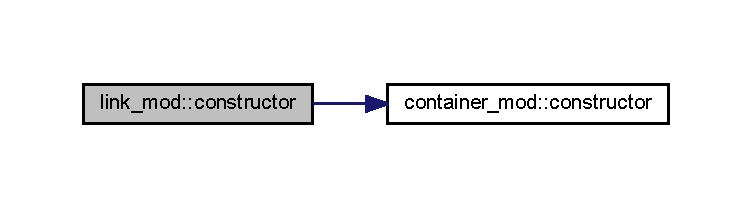
\includegraphics[width=350pt]{namespacelink__mod_ac5b4f1702d8edb10a4559f6f371dc797_cgraph}
\end{center}
\end{figure}
\mbox{\Hypertarget{namespacelink__mod_aa2c8d19ee91797e19464fc7589cc2c39}\label{namespacelink__mod_aa2c8d19ee91797e19464fc7589cc2c39}} 
\index{link\+\_\+mod@{link\+\_\+mod}!getvalue@{getvalue}}
\index{getvalue@{getvalue}!link\+\_\+mod@{link\+\_\+mod}}
\subsubsection{\texorpdfstring{getvalue()}{getvalue()}}
{\footnotesize\ttfamily class($\ast$) function, pointer link\+\_\+mod\+::getvalue (\begin{DoxyParamCaption}\item[{class(\mbox{\hyperlink{structlink__mod_1_1link}{link}})}]{this }\end{DoxyParamCaption})\hspace{0.3cm}{\ttfamily [private]}}



Method that returns a pointer to the values stored in the container in this link. 

\begin{DoxyAuthor}{Author}
Ricardo Birjukovs Canelas -\/ M\+A\+R\+E\+T\+EC 
\end{DoxyAuthor}


Definition at line 67 of file link.\+f90.


\begin{DoxyCode}
67     \textcolor{keywordtype}{class}(link) :: this
68     \textcolor{keywordtype}{class}(*), \textcolor{keywordtype}{pointer} :: getValue
69     getvalue => this%getContent()
\end{DoxyCode}
\mbox{\Hypertarget{namespacelink__mod_a2d776121ed0138aba8b3d166938c964f}\label{namespacelink__mod_a2d776121ed0138aba8b3d166938c964f}} 
\index{link\+\_\+mod@{link\+\_\+mod}!nextlink@{nextlink}}
\index{nextlink@{nextlink}!link\+\_\+mod@{link\+\_\+mod}}
\subsubsection{\texorpdfstring{nextlink()}{nextlink()}}
{\footnotesize\ttfamily class(\mbox{\hyperlink{structlink__mod_1_1link}{link}}) function, pointer link\+\_\+mod\+::nextlink (\begin{DoxyParamCaption}\item[{class(\mbox{\hyperlink{structlink__mod_1_1link}{link}})}]{this }\end{DoxyParamCaption})\hspace{0.3cm}{\ttfamily [private]}}



Method that returns a pointer to the next link in a list. 

\begin{DoxyAuthor}{Author}
Ricardo Birjukovs Canelas -\/ M\+A\+R\+E\+T\+EC 
\end{DoxyAuthor}


Definition at line 78 of file link.\+f90.


\begin{DoxyCode}
78     \textcolor{keywordtype}{class}(link) :: this
79     \textcolor{keywordtype}{class}(link), \textcolor{keywordtype}{pointer} :: nextLink
80     nextlink => this%next
\end{DoxyCode}
\mbox{\Hypertarget{namespacelink__mod_a2d23022ef22049f8340099b6960d8d5d}\label{namespacelink__mod_a2d23022ef22049f8340099b6960d8d5d}} 
\index{link\+\_\+mod@{link\+\_\+mod}!previouslink@{previouslink}}
\index{previouslink@{previouslink}!link\+\_\+mod@{link\+\_\+mod}}
\subsubsection{\texorpdfstring{previouslink()}{previouslink()}}
{\footnotesize\ttfamily class(\mbox{\hyperlink{structlink__mod_1_1link}{link}}) function, pointer link\+\_\+mod\+::previouslink (\begin{DoxyParamCaption}\item[{class(\mbox{\hyperlink{structlink__mod_1_1link}{link}})}]{this }\end{DoxyParamCaption})\hspace{0.3cm}{\ttfamily [private]}}



Method that returns a pointer to the previous link in a list. 

\begin{DoxyAuthor}{Author}
Ricardo Birjukovs Canelas -\/ M\+A\+R\+E\+T\+EC 
\end{DoxyAuthor}


Definition at line 89 of file link.\+f90.


\begin{DoxyCode}
89     \textcolor{keywordtype}{class}(link) :: this
90     \textcolor{keywordtype}{class}(link), \textcolor{keywordtype}{pointer} :: previousLink
91     previouslink => this%previous
\end{DoxyCode}
\mbox{\Hypertarget{namespacelink__mod_ae2d89f23eb8cf4b8065b8a39e9902a22}\label{namespacelink__mod_ae2d89f23eb8cf4b8065b8a39e9902a22}} 
\index{link\+\_\+mod@{link\+\_\+mod}!removelink@{removelink}}
\index{removelink@{removelink}!link\+\_\+mod@{link\+\_\+mod}}
\subsubsection{\texorpdfstring{removelink()}{removelink()}}
{\footnotesize\ttfamily subroutine link\+\_\+mod\+::removelink (\begin{DoxyParamCaption}\item[{class(\mbox{\hyperlink{structlink__mod_1_1link}{link}}), intent(inout)}]{this }\end{DoxyParamCaption})\hspace{0.3cm}{\ttfamily [private]}}



Method to remove a link in a list. 

\begin{DoxyAuthor}{Author}
Ricardo Birjukovs Canelas -\/ M\+A\+R\+E\+T\+EC 
\end{DoxyAuthor}


Definition at line 122 of file link.\+f90.


\begin{DoxyCode}
122     \textcolor{keywordtype}{class}(link), \textcolor{keywordtype}{intent(inout)} :: this
123     \textcolor{keyword}{call }this%deleteContent()
\end{DoxyCode}
\mbox{\Hypertarget{namespacelink__mod_a0dd2fe581e8d566faf03fc7ebd2f8524}\label{namespacelink__mod_a0dd2fe581e8d566faf03fc7ebd2f8524}} 
\index{link\+\_\+mod@{link\+\_\+mod}!setnextlink@{setnextlink}}
\index{setnextlink@{setnextlink}!link\+\_\+mod@{link\+\_\+mod}}
\subsubsection{\texorpdfstring{setnextlink()}{setnextlink()}}
{\footnotesize\ttfamily subroutine link\+\_\+mod\+::setnextlink (\begin{DoxyParamCaption}\item[{class(\mbox{\hyperlink{structlink__mod_1_1link}{link}})}]{this,  }\item[{class(\mbox{\hyperlink{structlink__mod_1_1link}{link}}), pointer}]{next }\end{DoxyParamCaption})\hspace{0.3cm}{\ttfamily [private]}}



Method to set the next link in a list. 

\begin{DoxyAuthor}{Author}
Ricardo Birjukovs Canelas -\/ M\+A\+R\+E\+T\+EC 
\end{DoxyAuthor}


Definition at line 100 of file link.\+f90.


\begin{DoxyCode}
100     \textcolor{keywordtype}{class}(link) :: this
101     \textcolor{keywordtype}{class}(link), \textcolor{keywordtype}{pointer} :: next
102     this%next => next
\end{DoxyCode}
\mbox{\Hypertarget{namespacelink__mod_ad0d413cb7907fdcf6561639cdd03481a}\label{namespacelink__mod_ad0d413cb7907fdcf6561639cdd03481a}} 
\index{link\+\_\+mod@{link\+\_\+mod}!setpreviouslink@{setpreviouslink}}
\index{setpreviouslink@{setpreviouslink}!link\+\_\+mod@{link\+\_\+mod}}
\subsubsection{\texorpdfstring{setpreviouslink()}{setpreviouslink()}}
{\footnotesize\ttfamily subroutine link\+\_\+mod\+::setpreviouslink (\begin{DoxyParamCaption}\item[{class(\mbox{\hyperlink{structlink__mod_1_1link}{link}})}]{this,  }\item[{class(\mbox{\hyperlink{structlink__mod_1_1link}{link}}), pointer}]{prev }\end{DoxyParamCaption})\hspace{0.3cm}{\ttfamily [private]}}



Method to set the previous link in a list. 

\begin{DoxyAuthor}{Author}
Ricardo Birjukovs Canelas -\/ M\+A\+R\+E\+T\+EC 
\end{DoxyAuthor}


Definition at line 111 of file link.\+f90.


\begin{DoxyCode}
111     \textcolor{keywordtype}{class}(link) :: this
112     \textcolor{keywordtype}{class}(link), \textcolor{keywordtype}{pointer} :: prev
113     this%previous => prev
\end{DoxyCode}

\hypertarget{namespacemtimeseriesparser__mod}{}\section{mtimeseriesparser\+\_\+mod Module Reference}
\label{namespacemtimeseriesparser__mod}\index{mtimeseriesparser\+\_\+mod@{mtimeseriesparser\+\_\+mod}}


Module defining a M\+O\+H\+ID time series parsing class and methods, encapsulates the M\+O\+H\+ID Module\+Time\+Serie module, from Base 1.  


\subsection*{Data Types}
\begin{DoxyCompactItemize}
\item 
type \mbox{\hyperlink{structmtimeseriesparser__mod_1_1mtimeseriesparser__class}{mtimeseriesparser\+\_\+class}}
\end{DoxyCompactItemize}
\subsection*{Functions/\+Subroutines}
\begin{DoxyCompactItemize}
\item 
subroutine \mbox{\hyperlink{namespacemtimeseriesparser__mod_abbc158c89dfc5a988984c1e9acd6dc48}{getfile}} (self, filename, var\+List)
\begin{DoxyCompactList}\small\item\em Method that parses a M\+O\+H\+ID time series file and stores the data internaly. \end{DoxyCompactList}\item 
subroutine \mbox{\hyperlink{namespacemtimeseriesparser__mod_a99a6266d1929abd218dd968d5c27a30d}{getdatabylabel}} (self, data\+Name, data\+\_\+out)
\begin{DoxyCompactList}\small\item\em Method that gets data from a column of a M\+O\+H\+ID time series file, given a string with a variable name. \end{DoxyCompactList}\end{DoxyCompactItemize}


\subsection{Detailed Description}
Module defining a M\+O\+H\+ID time series parsing class and methods, encapsulates the M\+O\+H\+ID Module\+Time\+Serie module, from Base 1. 

\begin{DoxyAuthor}{Author}
Ricardo Birjukovs Canelas 
\end{DoxyAuthor}


\subsection{Function/\+Subroutine Documentation}
\mbox{\Hypertarget{namespacemtimeseriesparser__mod_a99a6266d1929abd218dd968d5c27a30d}\label{namespacemtimeseriesparser__mod_a99a6266d1929abd218dd968d5c27a30d}} 
\index{mtimeseriesparser\+\_\+mod@{mtimeseriesparser\+\_\+mod}!getdatabylabel@{getdatabylabel}}
\index{getdatabylabel@{getdatabylabel}!mtimeseriesparser\+\_\+mod@{mtimeseriesparser\+\_\+mod}}
\subsubsection{\texorpdfstring{getdatabylabel()}{getdatabylabel()}}
{\footnotesize\ttfamily subroutine mtimeseriesparser\+\_\+mod\+::getdatabylabel (\begin{DoxyParamCaption}\item[{class(\mbox{\hyperlink{structmtimeseriesparser__mod_1_1mtimeseriesparser__class}{mtimeseriesparser\+\_\+class}}), intent(in)}]{self,  }\item[{type(string), intent(in)}]{data\+Name,  }\item[{real(prec), dimension(\+:), intent(out), allocatable}]{data\+\_\+out }\end{DoxyParamCaption})\hspace{0.3cm}{\ttfamily [private]}}



Method that gets data from a column of a M\+O\+H\+ID time series file, given a string with a variable name. 

\begin{DoxyAuthor}{Author}
Ricardo Birjukovs Canelas -\/ M\+A\+R\+E\+T\+EC 
\end{DoxyAuthor}

\begin{DoxyParams}[1]{Parameters}
\mbox{\tt in}  & {\em self,data\+Name,data\+\_\+out} & \\
\hline
\end{DoxyParams}


Definition at line 144 of file M\+Timeseries\+Parser.\+f90.


\begin{DoxyCode}
144     \textcolor{keywordtype}{class}(mTimeSeriesParser\_class), \textcolor{keywordtype}{intent(in)} :: self
145     \textcolor{keywordtype}{type}(string), \textcolor{keywordtype}{intent(in)} :: dataName
146     \textcolor{keywordtype}{real(prec)}, \textcolor{keywordtype}{dimension(:)}, \textcolor{keywordtype}{allocatable}, \textcolor{keywordtype}{intent(out)} :: data\_out
147     \textcolor{keywordtype}{integer} :: idx
148     \textcolor{keywordtype}{type}(string) :: outext
149 
150     idx = utils%find\_str(self%varName, dataname)
151     \textcolor{keywordflow}{if} (idx == mv\_int) \textcolor{keywordflow}{then}
152         outext = \textcolor{stringliteral}{'[MTimeSeriesParser::getDataByLabel]: File '}//self%filename//\textcolor{stringliteral}{' doesn'}\textcolor{stringliteral}{'t list variable
       representing '}//dataname//\textcolor{stringliteral}{', stoping'}
153         \textcolor{keyword}{call }log%put(outext)
154         stop
155 \textcolor{keywordflow}{    end if}
156     \textcolor{keyword}{allocate}(data\_out(\textcolor{keyword}{size}(self%dataMatrix,1)))
157     data\_out = self%dataMatrix(:,idx)
158 
\end{DoxyCode}
\mbox{\Hypertarget{namespacemtimeseriesparser__mod_abbc158c89dfc5a988984c1e9acd6dc48}\label{namespacemtimeseriesparser__mod_abbc158c89dfc5a988984c1e9acd6dc48}} 
\index{mtimeseriesparser\+\_\+mod@{mtimeseriesparser\+\_\+mod}!getfile@{getfile}}
\index{getfile@{getfile}!mtimeseriesparser\+\_\+mod@{mtimeseriesparser\+\_\+mod}}
\subsubsection{\texorpdfstring{getfile()}{getfile()}}
{\footnotesize\ttfamily subroutine mtimeseriesparser\+\_\+mod\+::getfile (\begin{DoxyParamCaption}\item[{class(\mbox{\hyperlink{structmtimeseriesparser__mod_1_1mtimeseriesparser__class}{mtimeseriesparser\+\_\+class}}), intent(inout)}]{self,  }\item[{type(string), intent(in)}]{filename,  }\item[{type(string), dimension(\+:), intent(in), optional}]{var\+List }\end{DoxyParamCaption})\hspace{0.3cm}{\ttfamily [private]}}



Method that parses a M\+O\+H\+ID time series file and stores the data internaly. 

\begin{DoxyAuthor}{Author}
Ricardo Birjukovs Canelas -\/ M\+A\+R\+E\+T\+EC 
\end{DoxyAuthor}

\begin{DoxyParams}[1]{Parameters}
\mbox{\tt in}  & {\em self,filename,var\+List} & \\
\hline
\end{DoxyParams}


Definition at line 54 of file M\+Timeseries\+Parser.\+f90.


\begin{DoxyCode}
54     \textcolor{keywordtype}{class}(mTimeSeriesParser\_class), \textcolor{keywordtype}{intent(inout)} :: self
55     \textcolor{keywordtype}{type}(string), \textcolor{keywordtype}{intent(in)} :: filename
56     \textcolor{keywordtype}{type}(string), \textcolor{keywordtype}{dimension(:)}, \textcolor{keywordtype}{optional}, \textcolor{keywordtype}{intent(in)} :: varList
57     \textcolor{keywordtype}{integer} :: id, STAT\_CALL, i, j
58     \textcolor{keywordtype}{integer} :: nColumns, nVals
59     \textcolor{keywordtype}{type}(string) :: outext
60     \textcolor{keywordtype}{type}(string) :: header, temp
61     \textcolor{keywordtype}{type}(datetime) :: initialDateTime
62     \textcolor{keywordtype}{type}(timedelta) :: dateTimeOffset
63     \textcolor{keywordtype}{real(prec)} :: timeOffset
64     \textcolor{keywordtype}{logical} :: found
65     \textcolor{keywordtype}{character(len=line\_length)} :: mHeader
66     \textcolor{keywordtype}{real}, \textcolor{keywordtype}{dimension(:,:)}, \textcolor{keywordtype}{pointer} :: mDataMatrix
67     \textcolor{keywordtype}{type}(T\_Time) :: mInitialDate
68     \textcolor{keywordtype}{real} :: mDate(6)
69 
70     outext = \textcolor{stringliteral}{'-> Reading MOHID Time Series file '}// filename
71     \textcolor{keyword}{call }log%put(outext)
72     id = 0
73     \textcolor{keyword}{call }starttimeserieinput(id, filename%chars(), stat = stat\_call)
74     \textcolor{keywordflow}{if} (stat\_call /= success\_) \textcolor{keywordflow}{then}
75         outext = \textcolor{stringliteral}{'[MTimeSeriesParser::getFile]: Cannot open '}//filename//\textcolor{stringliteral}{' file, stoping'}
76         \textcolor{keyword}{call }log%put(outext)
77         stop
78 \textcolor{keywordflow}{    end if}
79 
80     \textcolor{comment}{!getting data limits and header}
81     \textcolor{keyword}{call }gettimeseriedatacolumns(id, ncolumns, stat = stat\_call)
82     \textcolor{keyword}{call }gettimeseriedatavalues(id, nvals, stat = stat\_call)
83     \textcolor{keyword}{call }gettimeserieheader(id, mheader, stat = stat\_call)
84     \textcolor{comment}{!getting actual data matrix, already with time in seconds from date in file}
85     \textcolor{keyword}{allocate}(mdatamatrix(nvals, ncolumns))
86     \textcolor{keyword}{call }gettimeseriedatamatrix(id, mdatamatrix, stat = stat\_call)
87     \textcolor{comment}{!getting initial date and offseting to match simulation time dimension}
88     \textcolor{keyword}{call }gettimeserieinitialdata(id, minitialdate, stat = stat\_call)
89     \textcolor{keyword}{call }extractdate(minitialdate, mdate(1), mdate(2), mdate(3), mdate(4), mdate(5), mdate(6))
90     initialdatetime = utils%getDateTimeFromDate(int(mdate))
91     datetimeoffset = initialdatetime - globals%SimTime%StartDate
92     timeoffset = datetimeoffset%total\_seconds()
93     mdatamatrix(:,1) = mdatamatrix(:,1) + timeoffset \textcolor{comment}{!correcting for current time dimension}
94     \textcolor{comment}{!storing data in parser object}
95     \textcolor{keyword}{allocate}(self%dataMatrix(nvals, ncolumns))
96     self%dataMatrix = mdatamatrix
97     \textcolor{comment}{!cleaning up the header and getting individual data labels}
98     header = mheader
99     temp = header%replace(old=\textcolor{stringliteral}{'!'}, new=\textcolor{stringliteral}{''})
100     temp = temp%replace(old=\textcolor{stringliteral}{'  '}, new=\textcolor{stringliteral}{' '})
101     \textcolor{keywordflow}{do} \textcolor{keywordflow}{while} (temp/= header)
102         header = temp
103         temp = header%replace(old=\textcolor{stringliteral}{'  '}, new=\textcolor{stringliteral}{' '})
104 \textcolor{keywordflow}{    end do}
105     \textcolor{comment}{!spliting and storing in parser object}
106     \textcolor{keyword}{call }header%split(tokens=self%varName, sep=\textcolor{stringliteral}{' '})
107     \textcolor{comment}{!searching and replacing the variable names with required simulation names}
108     \textcolor{keywordflow}{if} (\textcolor{keyword}{present}(varlist)) \textcolor{keywordflow}{then}
109         \textcolor{keywordflow}{do} i=1, \textcolor{keyword}{size}(varlist)
110             found = .false.
111             \textcolor{keywordflow}{do} j=1,\textcolor{keyword}{size}(self%varName)
112                 \textcolor{keywordflow}{if} (globals%Var%getVarSimName(self%varName(j)) == varlist(i)) \textcolor{keywordflow}{then}
113                     self%varName(j) = globals%Var%getVarSimName(self%varName(j))
114                     found = .true.
115                     \textcolor{keywordflow}{exit}
116 \textcolor{keywordflow}{                end if}
117 \textcolor{keywordflow}{            end do}
118             \textcolor{keywordflow}{if} (.not.found) \textcolor{keywordflow}{then}
119                 outext = \textcolor{stringliteral}{'[MTimeSeriesParser::getFile]: File '}//filename//\textcolor{stringliteral}{' doesn'}\textcolor{stringliteral}{'t list variable
       representing '}//varlist(i)//\textcolor{stringliteral}{', stoping'}
120                 \textcolor{keyword}{call }log%put(outext)
121                 stop
122 \textcolor{keywordflow}{            end if}
123 \textcolor{keywordflow}{        end do}
124 \textcolor{keywordflow}{    end if}
125     self%filename = filename
126 
127     \textcolor{comment}{!destroying the MOHID Time Series module instance}
128     \textcolor{keyword}{call }killtimeserie(id, stat = stat\_call)
129     
130     \textcolor{comment}{!print*, self%filename}
131     \textcolor{comment}{!print*, self%varName}
132     \textcolor{comment}{!print*, self%dataMatrix}
133 
\end{DoxyCode}

\hypertarget{namespacenetcdfparser__mod}{}\section{netcdfparser\+\_\+mod Module Reference}
\label{namespacenetcdfparser__mod}\index{netcdfparser\+\_\+mod@{netcdfparser\+\_\+mod}}


Module that defines a netcdf file model class, responsible for abstracting the parsing of netcdf files. Each object of this class is responsible for one file, effectivelly representing it. The object should return the necessary data fields with corresponding meta data, such as names and units. An variable library is consulted when required, because even Net\+C\+DF CF compliance allows ambiguity.  


\subsection*{Data Types}
\begin{DoxyCompactItemize}
\item 
type \mbox{\hyperlink{structnetcdfparser__mod_1_1dim__t}{dim\+\_\+t}}
\item 
type \mbox{\hyperlink{structnetcdfparser__mod_1_1ncfile__class}{ncfile\+\_\+class}}
\begin{DoxyCompactList}\small\item\em A class that models a netcdf file. \end{DoxyCompactList}\item 
type \mbox{\hyperlink{structnetcdfparser__mod_1_1var__t}{var\+\_\+t}}
\end{DoxyCompactItemize}
\subsection*{Functions/\+Subroutines}
\begin{DoxyCompactItemize}
\item 
subroutine \mbox{\hyperlink{namespacenetcdfparser__mod_a57c39a4003778a6bf90cfd36b69380bc}{getfile}} (self, filename)
\begin{DoxyCompactList}\small\item\em Parse the netcdf file headers and assembles the file model. \end{DoxyCompactList}\item 
subroutine \mbox{\hyperlink{namespacenetcdfparser__mod_a741dd5b5985255e73aa9d3cf08755e91}{getncid}} (self)
\begin{DoxyCompactList}\small\item\em Opens the netcdf file, assigns the N\+C\+ID and checks for errors. \end{DoxyCompactList}\item 
subroutine \mbox{\hyperlink{namespacenetcdfparser__mod_a409f59662d71fb63e5fb5e057fdfd6ee}{getncglobalmetadata}} (self)
\begin{DoxyCompactList}\small\item\em Inquires the nc file for global metadata -\/ number of dimensions, variables and attributes. \end{DoxyCompactList}\item 
subroutine \mbox{\hyperlink{namespacenetcdfparser__mod_a46989199271acb6205cc61ac413d5a56}{getncvarmetadata}} (self)
\begin{DoxyCompactList}\small\item\em Inquires the nc file for variable metadata. \end{DoxyCompactList}\item 
subroutine \mbox{\hyperlink{namespacenetcdfparser__mod_a6354ee8b3c773cc7a5ad247ad1e34eeb}{getncdimmetadata}} (self)
\begin{DoxyCompactList}\small\item\em Inquires the nc file for dimension metadata. \end{DoxyCompactList}\item 
subroutine \mbox{\hyperlink{namespacenetcdfparser__mod_a0aea819b8a474ce2f4840d0bc44e95ec}{getvardimensions}} (self, var\+Name, dims\+Arrays)
\begin{DoxyCompactList}\small\item\em Reads the dimension fields from the nc file for a given variable. returns an array of scalar 1D fields, each with a name, units and data. \end{DoxyCompactList}\item 
subroutine \mbox{\hyperlink{namespacenetcdfparser__mod_aba877869db6bea7262d659133253cff7}{getvar}} (self, var\+Name, var\+Field, binary\+Var, alt\+Name, alt\+Units)
\begin{DoxyCompactList}\small\item\em Reads the fields from the nc file for a given variable. returns a generic field, with a name, units and data. \end{DoxyCompactList}\item 
type(\mbox{\hyperlink{structnetcdfparser__mod_1_1dim__t}{dim\+\_\+t}}) function \mbox{\hyperlink{namespacenetcdfparser__mod_a5fcd4b7fb27dbc9befd0a6fcfb9929a1}{getdimbydimid}} (self, dim\+ID)
\begin{DoxyCompactList}\small\item\em returns a dimension field metadata structure, given a dim\+ID \end{DoxyCompactList}\item 
subroutine \mbox{\hyperlink{namespacenetcdfparser__mod_a518627511cac4bf3dbc338bf3bfd5e24}{closefile}} (self)
\begin{DoxyCompactList}\small\item\em Close the netcdf file. \end{DoxyCompactList}\item 
subroutine \mbox{\hyperlink{namespacenetcdfparser__mod_ae1a034f6540ac7a1ce7d0e3831bb2f03}{check}} (self)
\begin{DoxyCompactList}\small\item\em Debug the netcdf error after a netcdf command. \end{DoxyCompactList}\item 
subroutine \mbox{\hyperlink{namespacenetcdfparser__mod_aeb48d33c014bae21b2fceaaa70cbdc67}{printncinfo}} (self)
\begin{DoxyCompactList}\small\item\em prints most of the file model metadata \end{DoxyCompactList}\item 
subroutine \mbox{\hyperlink{namespacenetcdfparser__mod_a6b57fa47d7bd796c75483216a51e5e04}{printvarsnc}} (self)
\begin{DoxyCompactList}\small\item\em print variable metadata \end{DoxyCompactList}\item 
subroutine \mbox{\hyperlink{namespacenetcdfparser__mod_ac01c000a97d23613684155708249ce89}{printdimsnc}} (self)
\begin{DoxyCompactList}\small\item\em print dimensions metadata \end{DoxyCompactList}\item 
subroutine \mbox{\hyperlink{namespacenetcdfparser__mod_af93319fde6cf6baedb7fe27bf3396e7b}{correctnctime}} (time\+Comments, time\+Array)
\begin{DoxyCompactList}\small\item\em corrects the time array to a more efficient format if needed. assumes netcdf comment as \textquotesingle{}seconds since 1981-\/01-\/01 00\+:00\+:00\textquotesingle{} \end{DoxyCompactList}\end{DoxyCompactItemize}


\subsection{Detailed Description}
Module that defines a netcdf file model class, responsible for abstracting the parsing of netcdf files. Each object of this class is responsible for one file, effectivelly representing it. The object should return the necessary data fields with corresponding meta data, such as names and units. An variable library is consulted when required, because even Net\+C\+DF CF compliance allows ambiguity. 

\begin{DoxyAuthor}{Author}
Daniel Garaboa Paz 
\end{DoxyAuthor}


\subsection{Function/\+Subroutine Documentation}
\mbox{\Hypertarget{namespacenetcdfparser__mod_ae1a034f6540ac7a1ce7d0e3831bb2f03}\label{namespacenetcdfparser__mod_ae1a034f6540ac7a1ce7d0e3831bb2f03}} 
\index{netcdfparser\+\_\+mod@{netcdfparser\+\_\+mod}!check@{check}}
\index{check@{check}!netcdfparser\+\_\+mod@{netcdfparser\+\_\+mod}}
\subsubsection{\texorpdfstring{check()}{check()}}
{\footnotesize\ttfamily subroutine netcdfparser\+\_\+mod\+::check (\begin{DoxyParamCaption}\item[{class(\mbox{\hyperlink{structnetcdfparser__mod_1_1ncfile__class}{ncfile\+\_\+class}}), intent(inout)}]{self }\end{DoxyParamCaption})\hspace{0.3cm}{\ttfamily [private]}}



Debug the netcdf error after a netcdf command. 

\begin{DoxyAuthor}{Author}
Daniel Garaboa Paz -\/ U\+SC 
\end{DoxyAuthor}

\begin{DoxyParams}[1]{Parameters}
\mbox{\tt in}  & {\em self} & \\
\hline
\end{DoxyParams}


Definition at line 444 of file Net\+C\+D\+Fparser.\+f90.


\begin{DoxyCode}
444     \textcolor{keywordtype}{class}(ncfile\_class), \textcolor{keywordtype}{intent(inout)} :: self
445     \textcolor{keywordtype}{type}(string) :: outext
446     \textcolor{keywordflow}{if}(self%status /= nf90\_noerr) \textcolor{keywordflow}{then}
447         outext = \textcolor{stringliteral}{'[NetCDFparser::check]: '}//trim(nf90\_strerror(self%status))//\textcolor{stringliteral}{', stoping'}
448         \textcolor{keyword}{call }log%put(outext)
449         stop
450 \textcolor{keywordflow}{    end if}
\end{DoxyCode}
\mbox{\Hypertarget{namespacenetcdfparser__mod_a518627511cac4bf3dbc338bf3bfd5e24}\label{namespacenetcdfparser__mod_a518627511cac4bf3dbc338bf3bfd5e24}} 
\index{netcdfparser\+\_\+mod@{netcdfparser\+\_\+mod}!closefile@{closefile}}
\index{closefile@{closefile}!netcdfparser\+\_\+mod@{netcdfparser\+\_\+mod}}
\subsubsection{\texorpdfstring{closefile()}{closefile()}}
{\footnotesize\ttfamily subroutine netcdfparser\+\_\+mod\+::closefile (\begin{DoxyParamCaption}\item[{class(\mbox{\hyperlink{structnetcdfparser__mod_1_1ncfile__class}{ncfile\+\_\+class}}), intent(inout)}]{self }\end{DoxyParamCaption})\hspace{0.3cm}{\ttfamily [private]}}



Close the netcdf file. 

\begin{DoxyAuthor}{Author}
Daniel Garaboa Paz -\/ U\+SC 
\end{DoxyAuthor}

\begin{DoxyParams}[1]{Parameters}
\mbox{\tt in}  & {\em self} & \\
\hline
\end{DoxyParams}


Definition at line 432 of file Net\+C\+D\+Fparser.\+f90.


\begin{DoxyCode}
432     \textcolor{keywordtype}{class}(ncfile\_class),\textcolor{keywordtype}{intent(inout)} :: self
433     self%status = nf90\_close(self%ncID)
434     \textcolor{keyword}{call }self%check()
\end{DoxyCode}
\mbox{\Hypertarget{namespacenetcdfparser__mod_af93319fde6cf6baedb7fe27bf3396e7b}\label{namespacenetcdfparser__mod_af93319fde6cf6baedb7fe27bf3396e7b}} 
\index{netcdfparser\+\_\+mod@{netcdfparser\+\_\+mod}!correctnctime@{correctnctime}}
\index{correctnctime@{correctnctime}!netcdfparser\+\_\+mod@{netcdfparser\+\_\+mod}}
\subsubsection{\texorpdfstring{correctnctime()}{correctnctime()}}
{\footnotesize\ttfamily subroutine netcdfparser\+\_\+mod\+::correctnctime (\begin{DoxyParamCaption}\item[{type(string), intent(inout)}]{time\+Comments,  }\item[{real(prec), dimension(\+:), intent(inout)}]{time\+Array }\end{DoxyParamCaption})\hspace{0.3cm}{\ttfamily [private]}}



corrects the time array to a more efficient format if needed. assumes netcdf comment as \textquotesingle{}seconds since 1981-\/01-\/01 00\+:00\+:00\textquotesingle{} 

\begin{DoxyAuthor}{Author}
Ricardo Birjukovs Canelas -\/ M\+A\+R\+E\+T\+EC 
\end{DoxyAuthor}

\begin{DoxyParams}[1]{Parameters}
\mbox{\tt in}  & {\em time\+Comments,time\+Array} & \\
\hline
\end{DoxyParams}


Definition at line 523 of file Net\+C\+D\+Fparser.\+f90.


\begin{DoxyCode}
523     \textcolor{keywordtype}{type}(string), \textcolor{keywordtype}{intent(inout)} :: timeComments
524     \textcolor{keywordtype}{real(prec)}, \textcolor{keywordtype}{dimension(:)}, \textcolor{keywordtype}{intent(inout)} :: timeArray
525     \textcolor{keywordtype}{integer} :: i
526     \textcolor{keywordtype}{type}(string), \textcolor{keywordtype}{allocatable} :: dc(:), dates(:), hours(:)
527     \textcolor{keywordtype}{type}(string) :: isoDateStr
528     \textcolor{keywordtype}{integer}, \textcolor{keywordtype}{dimension(6)} :: date
529     \textcolor{keywordtype}{type}(datetime) :: NCDate
530     \textcolor{keywordtype}{type}(timedelta) :: dateOffset
531     \textcolor{keywordtype}{type}(string) :: outext
532     \textcolor{keywordtype}{real(prec)} :: scale, offset
533 
534     \textcolor{keyword}{call }timecomments%split(tokens=dc, sep=\textcolor{stringliteral}{' '})
535     \textcolor{keywordflow}{if} (\textcolor{keyword}{size}(dc) == 4) \textcolor{keywordflow}{then}
536         scale = 1.0
537         \textcolor{keywordflow}{if} (dc(1) == \textcolor{stringliteral}{'seconds'}) scale = 1.0
538         \textcolor{keywordflow}{if} (dc(1) == \textcolor{stringliteral}{'hours'})   scale = 3600.0
539         \textcolor{keywordflow}{if} (dc(1) == \textcolor{stringliteral}{'days'})    scale = 3600.0*24.0
540         \textcolor{keywordflow}{if} (dc(1) == \textcolor{stringliteral}{'months'})  scale = 3600.0*24.0*30.0 \textcolor{comment}{!really hope no one gets such a brilliant idea as
       to use this as a time unit}
541         \textcolor{keywordflow}{if} (dc(1) == \textcolor{stringliteral}{'years'})   scale = 3600.0*24.0*30.0*12.0 \textcolor{comment}{!or this}
542         \textcolor{keyword}{call }dc(3)%split(tokens=dates, sep=\textcolor{stringliteral}{'-'})
543         \textcolor{keyword}{call }dc(4)%split(tokens=hours, sep=\textcolor{stringliteral}{':'})
544         isodatestr = dates(1)//\textcolor{stringliteral}{' '}//dates(2)//\textcolor{stringliteral}{' '}//dates(3)//\textcolor{stringliteral}{' '}//hours(1)//\textcolor{stringliteral}{' '}//hours(2)//\textcolor{stringliteral}{' '}//hours(3)
545         date = utils%getDateFromISOString(isodatestr)
546         ncdate = datetime(date(1),date(2),date(3),date(4),date(5),date(6))
547         dateoffset = globals%SimTime%StartDate - ncdate
548         offset = -dateoffset%total\_seconds()
549 
550         timearray = timearray*scale + offset
551         timecomments = \textcolor{stringliteral}{'seconds since '}//globals%SimTime%StartDate%isoformat(\textcolor{stringliteral}{' '})        
552     
553     \textcolor{keywordflow}{elseif} (\textcolor{keyword}{size}(dc) == 3) \textcolor{keywordflow}{then}
554         scale = 1.0
555         \textcolor{keywordflow}{if} (dc(1) == \textcolor{stringliteral}{'seconds'}) scale = 1.0
556         \textcolor{keywordflow}{if} (dc(1) == \textcolor{stringliteral}{'hours'})   scale = 3600.0
557         \textcolor{keywordflow}{if} (dc(1) == \textcolor{stringliteral}{'days'})    scale = 3600.0*24.0
558         \textcolor{keywordflow}{if} (dc(1) == \textcolor{stringliteral}{'months'})  scale = 3600.0*24.0*30.0 \textcolor{comment}{!really hope no one gets such a brilliant idea as
       to use this as a time unit}
559         \textcolor{keywordflow}{if} (dc(1) == \textcolor{stringliteral}{'years'})   scale = 3600.0*24.0*30.0*12.0 \textcolor{comment}{!or this}
560         \textcolor{keyword}{call }dc(3)%split(tokens=dates, sep=\textcolor{stringliteral}{'-'})
561         isodatestr = dates(1)//\textcolor{stringliteral}{' '}//dates(2)//\textcolor{stringliteral}{' '}//dates(3)//\textcolor{stringliteral}{' '}//\textcolor{stringliteral}{'00'}//\textcolor{stringliteral}{' '}//\textcolor{stringliteral}{'00'}//\textcolor{stringliteral}{' '}//\textcolor{stringliteral}{'00'}
562         date = utils%getDateFromISOString(isodatestr)
563         ncdate = datetime(date(1),date(2),date(3),date(4),date(5),date(6))
564         dateoffset = globals%SimTime%StartDate - ncdate
565         offset = -dateoffset%total\_seconds()
566         
567         timearray = timearray*scale + offset
568         timecomments = \textcolor{stringliteral}{'seconds since '}//globals%SimTime%StartDate%isoformat(\textcolor{stringliteral}{' '})
569         
570     \textcolor{keywordflow}{else}       
571 
572         outext = \textcolor{stringliteral}{'[NetCDF parser::correctNCTime]:WARNING - Time units may not be in the format *seconds
       since 1981-01-01 00:00:00*, you might have some problems in a few moments...'}
573         \textcolor{keyword}{call }log%put(outext)
574 \textcolor{keywordflow}{    end if}
575 
\end{DoxyCode}
Here is the caller graph for this function\+:\nopagebreak
\begin{figure}[H]
\begin{center}
\leavevmode
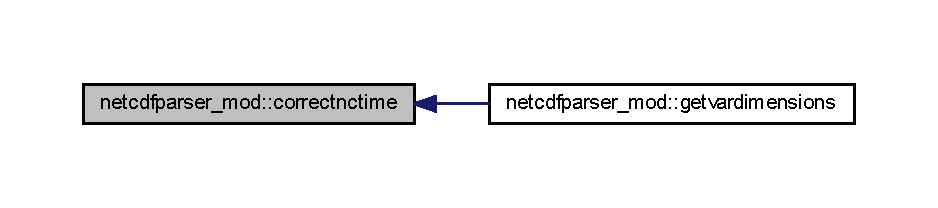
\includegraphics[width=350pt]{namespacenetcdfparser__mod_af93319fde6cf6baedb7fe27bf3396e7b_icgraph}
\end{center}
\end{figure}
\mbox{\Hypertarget{namespacenetcdfparser__mod_a5fcd4b7fb27dbc9befd0a6fcfb9929a1}\label{namespacenetcdfparser__mod_a5fcd4b7fb27dbc9befd0a6fcfb9929a1}} 
\index{netcdfparser\+\_\+mod@{netcdfparser\+\_\+mod}!getdimbydimid@{getdimbydimid}}
\index{getdimbydimid@{getdimbydimid}!netcdfparser\+\_\+mod@{netcdfparser\+\_\+mod}}
\subsubsection{\texorpdfstring{getdimbydimid()}{getdimbydimid()}}
{\footnotesize\ttfamily type(\mbox{\hyperlink{structnetcdfparser__mod_1_1dim__t}{dim\+\_\+t}}) function netcdfparser\+\_\+mod\+::getdimbydimid (\begin{DoxyParamCaption}\item[{class(\mbox{\hyperlink{structnetcdfparser__mod_1_1ncfile__class}{ncfile\+\_\+class}}), intent(inout)}]{self,  }\item[{integer, intent(in)}]{dim\+ID }\end{DoxyParamCaption})\hspace{0.3cm}{\ttfamily [private]}}



returns a dimension field metadata structure, given a dim\+ID 

\begin{DoxyAuthor}{Author}
Ricardo Birjukovs Canelas -\/ M\+A\+R\+E\+T\+EC 
\end{DoxyAuthor}

\begin{DoxyParams}[1]{Parameters}
\mbox{\tt in}  & {\em self,dim\+ID} & \\
\hline
\end{DoxyParams}


Definition at line 402 of file Net\+C\+D\+Fparser.\+f90.


\begin{DoxyCode}
402     \textcolor{keywordtype}{class}(ncfile\_class), \textcolor{keywordtype}{intent(inout)} :: self
403     \textcolor{keywordtype}{integer}, \textcolor{keywordtype}{intent(in)} :: dimID
404     \textcolor{keywordtype}{integer} :: i
405     \textcolor{keywordtype}{logical} :: found
406     \textcolor{keywordtype}{type}(string) :: outext
407 
408     found = .false.
409     \textcolor{keywordflow}{do} i=1, self%nDims
410         \textcolor{keywordflow}{if} (dimid == self%dimData(i)%dimid) \textcolor{keywordflow}{then}
411             found = .true.
412             getdimbydimid = self%dimData(i)
413             \textcolor{keywordflow}{return}
414 \textcolor{keywordflow}{        end if}
415 \textcolor{keywordflow}{    end do}
416     \textcolor{keywordflow}{if} (.not.found) \textcolor{keywordflow}{then}
417         outext = dimid
418         outext = \textcolor{stringliteral}{'[NetCDFparser::getDimByDimID]: dimension with ID='}//outext//\textcolor{stringliteral}{' not found. Stopping'}
419         \textcolor{keyword}{call }log%put(outext)
420         stop
421 \textcolor{keywordflow}{    end if}
422 
\end{DoxyCode}
\mbox{\Hypertarget{namespacenetcdfparser__mod_a57c39a4003778a6bf90cfd36b69380bc}\label{namespacenetcdfparser__mod_a57c39a4003778a6bf90cfd36b69380bc}} 
\index{netcdfparser\+\_\+mod@{netcdfparser\+\_\+mod}!getfile@{getfile}}
\index{getfile@{getfile}!netcdfparser\+\_\+mod@{netcdfparser\+\_\+mod}}
\subsubsection{\texorpdfstring{getfile()}{getfile()}}
{\footnotesize\ttfamily subroutine netcdfparser\+\_\+mod\+::getfile (\begin{DoxyParamCaption}\item[{class(\mbox{\hyperlink{structnetcdfparser__mod_1_1ncfile__class}{ncfile\+\_\+class}}), intent(inout)}]{self,  }\item[{type(string), intent(in)}]{filename }\end{DoxyParamCaption})\hspace{0.3cm}{\ttfamily [private]}}



Parse the netcdf file headers and assembles the file model. 

\begin{DoxyAuthor}{Author}
Ricardo Birjukovs Canelas -\/ M\+A\+R\+E\+T\+EC 
\end{DoxyAuthor}

\begin{DoxyParams}[1]{Parameters}
\mbox{\tt in}  & {\em self,filename} & \\
\hline
\end{DoxyParams}


Definition at line 101 of file Net\+C\+D\+Fparser.\+f90.


\begin{DoxyCode}
101     \textcolor{keywordtype}{class}(ncfile\_class), \textcolor{keywordtype}{intent(inout)} :: self
102     \textcolor{keywordtype}{type}(string), \textcolor{keywordtype}{intent(in)} :: filename
103     \textcolor{keywordtype}{integer} :: i
104     self%filename = filename
105     \textcolor{keyword}{call }self%getNCid()
106     \textcolor{keyword}{call }self%getNCglobalMetadata()
107     \textcolor{keyword}{call }self%getNCVarMetadata()
108     \textcolor{keyword}{call }self%getNCDimMetadata()
\end{DoxyCode}
\mbox{\Hypertarget{namespacenetcdfparser__mod_a6354ee8b3c773cc7a5ad247ad1e34eeb}\label{namespacenetcdfparser__mod_a6354ee8b3c773cc7a5ad247ad1e34eeb}} 
\index{netcdfparser\+\_\+mod@{netcdfparser\+\_\+mod}!getncdimmetadata@{getncdimmetadata}}
\index{getncdimmetadata@{getncdimmetadata}!netcdfparser\+\_\+mod@{netcdfparser\+\_\+mod}}
\subsubsection{\texorpdfstring{getncdimmetadata()}{getncdimmetadata()}}
{\footnotesize\ttfamily subroutine netcdfparser\+\_\+mod\+::getncdimmetadata (\begin{DoxyParamCaption}\item[{class(\mbox{\hyperlink{structnetcdfparser__mod_1_1ncfile__class}{ncfile\+\_\+class}}), intent(inout)}]{self }\end{DoxyParamCaption})\hspace{0.3cm}{\ttfamily [private]}}



Inquires the nc file for dimension metadata. 

\begin{DoxyAuthor}{Author}
Ricardo Birjukovs Canelas -\/ M\+A\+R\+E\+T\+EC 
\end{DoxyAuthor}

\begin{DoxyParams}[1]{Parameters}
\mbox{\tt in}  & {\em self} & \\
\hline
\end{DoxyParams}


Definition at line 178 of file Net\+C\+D\+Fparser.\+f90.


\begin{DoxyCode}
178     \textcolor{keywordtype}{class}(ncfile\_class), \textcolor{keywordtype}{intent(inout)} :: self
179     \textcolor{keywordtype}{integer} :: i, j, dimLength
180     \textcolor{keywordtype}{character(CHAR\_LEN)} :: dimName
181     \textcolor{keyword}{allocate}(self%dimData(self%nDims))
182     \textcolor{keywordflow}{do} i=1, self%nDims
183         self%status = nf90\_inquire\_dimension(self%ncID, i, dimname, dimlength)
184         \textcolor{keyword}{call }self%check()
185         self%dimData(i)%name = trim(dimname)
186         self%dimData(i)%simName = globals%Var%getVarSimName(self%dimData(i)%name)
187         self%dimData(i)%length = dimlength
188         self%status = nf90\_inq\_dimid(self%ncID, self%dimData(i)%name%chars(), self%dimData(i)%dimid)
189         \textcolor{keyword}{call }self%check()
190         \textcolor{keywordflow}{do} j=1, self%nVars
191             \textcolor{keywordflow}{if} (self%dimData(i)%name == self%varData(j)%name) \textcolor{keywordflow}{then}
192                 self%dimData(i)%units = self%varData(j)%units
193                 self%dimData(i)%varid = self%varData(j)%varid
194                 \textcolor{keywordflow}{exit}
195 \textcolor{keywordflow}{            end if}
196 \textcolor{keywordflow}{        end do}
197 \textcolor{keywordflow}{    end do}
\end{DoxyCode}
\mbox{\Hypertarget{namespacenetcdfparser__mod_a409f59662d71fb63e5fb5e057fdfd6ee}\label{namespacenetcdfparser__mod_a409f59662d71fb63e5fb5e057fdfd6ee}} 
\index{netcdfparser\+\_\+mod@{netcdfparser\+\_\+mod}!getncglobalmetadata@{getncglobalmetadata}}
\index{getncglobalmetadata@{getncglobalmetadata}!netcdfparser\+\_\+mod@{netcdfparser\+\_\+mod}}
\subsubsection{\texorpdfstring{getncglobalmetadata()}{getncglobalmetadata()}}
{\footnotesize\ttfamily subroutine netcdfparser\+\_\+mod\+::getncglobalmetadata (\begin{DoxyParamCaption}\item[{class(\mbox{\hyperlink{structnetcdfparser__mod_1_1ncfile__class}{ncfile\+\_\+class}}), intent(inout)}]{self }\end{DoxyParamCaption})\hspace{0.3cm}{\ttfamily [private]}}



Inquires the nc file for global metadata -\/ number of dimensions, variables and attributes. 

\begin{DoxyAuthor}{Author}
Ricardo Birjukovs Canelas -\/ M\+A\+R\+E\+T\+EC 
\end{DoxyAuthor}

\begin{DoxyParams}[1]{Parameters}
\mbox{\tt in}  & {\em self} & \\
\hline
\end{DoxyParams}


Definition at line 131 of file Net\+C\+D\+Fparser.\+f90.


\begin{DoxyCode}
131     \textcolor{keywordtype}{class}(ncfile\_class), \textcolor{keywordtype}{intent(inout)} :: self
132     self%status = nf90\_inquire(self%ncID, self%nDims, self%nVars, self%nAtt, self%uDimID)
133     \textcolor{keyword}{call }self%check()
\end{DoxyCode}
\mbox{\Hypertarget{namespacenetcdfparser__mod_a741dd5b5985255e73aa9d3cf08755e91}\label{namespacenetcdfparser__mod_a741dd5b5985255e73aa9d3cf08755e91}} 
\index{netcdfparser\+\_\+mod@{netcdfparser\+\_\+mod}!getncid@{getncid}}
\index{getncid@{getncid}!netcdfparser\+\_\+mod@{netcdfparser\+\_\+mod}}
\subsubsection{\texorpdfstring{getncid()}{getncid()}}
{\footnotesize\ttfamily subroutine netcdfparser\+\_\+mod\+::getncid (\begin{DoxyParamCaption}\item[{class(\mbox{\hyperlink{structnetcdfparser__mod_1_1ncfile__class}{ncfile\+\_\+class}}), intent(inout)}]{self }\end{DoxyParamCaption})\hspace{0.3cm}{\ttfamily [private]}}



Opens the netcdf file, assigns the N\+C\+ID and checks for errors. 

\begin{DoxyAuthor}{Author}
Daniel Garaboa Paz -\/ U\+SC 
\end{DoxyAuthor}

\begin{DoxyParams}[1]{Parameters}
\mbox{\tt in}  & {\em self} & \\
\hline
\end{DoxyParams}


Definition at line 118 of file Net\+C\+D\+Fparser.\+f90.


\begin{DoxyCode}
118     \textcolor{keywordtype}{class}(ncfile\_class), \textcolor{keywordtype}{intent(inout)} :: self
119     self%status = nf90\_open(trim(self%filename%chars()), nf90\_nowrite, self%ncID)
120     \textcolor{keyword}{call }self%check()
\end{DoxyCode}
\mbox{\Hypertarget{namespacenetcdfparser__mod_a46989199271acb6205cc61ac413d5a56}\label{namespacenetcdfparser__mod_a46989199271acb6205cc61ac413d5a56}} 
\index{netcdfparser\+\_\+mod@{netcdfparser\+\_\+mod}!getncvarmetadata@{getncvarmetadata}}
\index{getncvarmetadata@{getncvarmetadata}!netcdfparser\+\_\+mod@{netcdfparser\+\_\+mod}}
\subsubsection{\texorpdfstring{getncvarmetadata()}{getncvarmetadata()}}
{\footnotesize\ttfamily subroutine netcdfparser\+\_\+mod\+::getncvarmetadata (\begin{DoxyParamCaption}\item[{class(\mbox{\hyperlink{structnetcdfparser__mod_1_1ncfile__class}{ncfile\+\_\+class}}), intent(inout)}]{self }\end{DoxyParamCaption})\hspace{0.3cm}{\ttfamily [private]}}



Inquires the nc file for variable metadata. 

\begin{DoxyAuthor}{Author}
Ricardo Birjukovs Canelas -\/ M\+A\+R\+E\+T\+EC 
\end{DoxyAuthor}

\begin{DoxyParams}[1]{Parameters}
\mbox{\tt in}  & {\em self} & \\
\hline
\end{DoxyParams}


Definition at line 143 of file Net\+C\+D\+Fparser.\+f90.


\begin{DoxyCode}
143     \textcolor{keywordtype}{class}(ncfile\_class), \textcolor{keywordtype}{intent(inout)} :: self
144     \textcolor{keywordtype}{integer} :: i, j, ndims, nAtts
145     \textcolor{keywordtype}{integer} :: dimids(self%nDims)
146     \textcolor{keywordtype}{integer} :: tempStatus
147     \textcolor{keywordtype}{character(CHAR\_LEN)} :: varName, units
148     \textcolor{keyword}{allocate}(self%varData(self%nVars))
149     \textcolor{keywordflow}{do} i=1, self%nVars
150         self%status = nf90\_inquire\_variable(self%ncID, i, varname, ndims=ndims, dimids=dimids, natts=natts)
151         \textcolor{keyword}{call }self%check()
152         self%varData(i)%name = trim(varname)
153         self%varData(i)%simName = globals%Var%getVarSimName(self%varData(i)%name)
154         self%varData(i)%varid = i
155         self%varData(i)%ndims = ndims
156         \textcolor{keyword}{allocate}(self%varData(i)%dimids(ndims))
157         self%varData(i)%dimids = dimids(1:ndims)
158         self%varData(i)%nAtts = natts
159         tempstatus = nf90\_get\_att(self%ncID, i, \textcolor{stringliteral}{'units'}, units)
160         \textcolor{keywordflow}{if} (tempstatus == -43) units = \textcolor{stringliteral}{"not set"}
161         self%varData(i)%units = trim(units)
162         tempstatus = nf90\_get\_att(self%ncID, i, \textcolor{stringliteral}{"scale\_factor"}, self%varData(i)%scale)
163         \textcolor{keywordflow}{if} (tempstatus == -43) self%varData(i)%scale = 1.0
164         tempstatus = nf90\_get\_att(self%ncID, i, \textcolor{stringliteral}{"add\_offset"}, self%varData(i)%offset)
165         \textcolor{keywordflow}{if} (tempstatus == -43) self%varData(i)%offset = 0.0
166         tempstatus = nf90\_get\_att(self%ncID, i, \textcolor{stringliteral}{"\_FillValue"}, self%varData(i)%fillvalue)
167         \textcolor{keywordflow}{if} (tempstatus == -43) self%varData(i)%fillvalue = mv
168 \textcolor{keywordflow}{    end do}
\end{DoxyCode}
\mbox{\Hypertarget{namespacenetcdfparser__mod_aba877869db6bea7262d659133253cff7}\label{namespacenetcdfparser__mod_aba877869db6bea7262d659133253cff7}} 
\index{netcdfparser\+\_\+mod@{netcdfparser\+\_\+mod}!getvar@{getvar}}
\index{getvar@{getvar}!netcdfparser\+\_\+mod@{netcdfparser\+\_\+mod}}
\subsubsection{\texorpdfstring{getvar()}{getvar()}}
{\footnotesize\ttfamily subroutine netcdfparser\+\_\+mod\+::getvar (\begin{DoxyParamCaption}\item[{class(\mbox{\hyperlink{structnetcdfparser__mod_1_1ncfile__class}{ncfile\+\_\+class}}), intent(inout)}]{self,  }\item[{type(string), intent(in)}]{var\+Name,  }\item[{type(generic\+\_\+field\+\_\+class), intent(out)}]{var\+Field,  }\item[{logical, intent(in), optional}]{binary\+Var,  }\item[{type(string), intent(in), optional}]{alt\+Name,  }\item[{type(string), intent(in), optional}]{alt\+Units }\end{DoxyParamCaption})\hspace{0.3cm}{\ttfamily [private]}}



Reads the fields from the nc file for a given variable. returns a generic field, with a name, units and data. 

\begin{DoxyAuthor}{Author}
Ricardo Birjukovs Canelas -\/ M\+A\+R\+E\+T\+EC 
\end{DoxyAuthor}

\begin{DoxyParams}[1]{Parameters}
\mbox{\tt in}  & {\em self,var\+Name,var\+Field,binary\+Var,alt\+Name,alt\+Units} & \\
\hline
\end{DoxyParams}


Definition at line 288 of file Net\+C\+D\+Fparser.\+f90.


\begin{DoxyCode}
288     \textcolor{keywordtype}{class}(ncfile\_class), \textcolor{keywordtype}{intent(inout)} :: self
289     \textcolor{keywordtype}{type}(string), \textcolor{keywordtype}{intent(in)} :: varName
290     \textcolor{keywordtype}{type}(generic\_field\_class), \textcolor{keywordtype}{intent(out)} :: varField
291     \textcolor{keywordtype}{logical}, \textcolor{keywordtype}{optional}, \textcolor{keywordtype}{intent(in)} :: binaryVar
292     \textcolor{keywordtype}{type}(string), \textcolor{keywordtype}{optional}, \textcolor{keywordtype}{intent(in)} :: altName, altUnits
293     \textcolor{keywordtype}{logical} :: bVar
294     \textcolor{keywordtype}{real(prec)}, \textcolor{keywordtype}{allocatable}, \textcolor{keywordtype}{dimension(:)} :: tempRealField1D
295     \textcolor{keywordtype}{real(prec)}, \textcolor{keywordtype}{allocatable}, \textcolor{keywordtype}{dimension(:,:,:)} :: tempRealField3D
296     \textcolor{keywordtype}{real(prec)}, \textcolor{keywordtype}{allocatable}, \textcolor{keywordtype}{dimension(:,:,:,:)} :: tempRealField4D
297     \textcolor{keywordtype}{type}(string) :: dimName, varUnits
298     \textcolor{keywordtype}{integer} :: i, j, k, id\_dim, first,last
299     \textcolor{keywordtype}{type}(dim\_t) :: tempDim
300     \textcolor{keywordtype}{integer}, \textcolor{keywordtype}{allocatable}, \textcolor{keywordtype}{dimension(:)} :: varShape
301     \textcolor{keywordtype}{type}(string) :: outext
302 
303     bvar= .false.
304     \textcolor{keywordflow}{if}(\textcolor{keyword}{present}(binaryvar)) bvar = binaryvar
305 
306     \textcolor{keywordflow}{do} i=1, self%nVars \textcolor{comment}{!going trough all variables}
307         \textcolor{keywordflow}{if} (self%varData(i)%simName == varname ) \textcolor{keywordflow}{then}   \textcolor{comment}{!found the requested var}
308             \textcolor{keyword}{allocate}(varshape(self%varData(i)%ndims))
309             \textcolor{keywordflow}{do} j=1, self%varData(i)%ndims   \textcolor{comment}{!going trough all of the variable dimensions}
310                 tempdim = self%getDimByDimID(self%varData(i)%dimids(j))
311                 varshape(j) = tempdim%length
312 \textcolor{keywordflow}{            end do}
313             \textcolor{keywordflow}{if}(self%varData(i)%ndims == 3) \textcolor{keywordflow}{then} \textcolor{comment}{!3D variable}
314                 \textcolor{keyword}{allocate}(temprealfield3d(varshape(1),varshape(2),varshape(3)))
315                 self%status = nf90\_get\_var(self%ncID, self%varData(i)%varid, temprealfield3d)
316                 \textcolor{keyword}{call }self%check()
317                 \textcolor{keywordflow}{if} (.not.bvar) \textcolor{keywordflow}{then}
318                     \textcolor{keywordflow}{where} (temprealfield3d == self%varData(i)%fillvalue) temprealfield3d = 0.0
319                     temprealfield3d = temprealfield3d*self%varData(i)%scale + self%varData(i)%offset \textcolor{comment}{!
       scale + offset transform}
320                 \textcolor{keywordflow}{else}
321                     \textcolor{keywordflow}{if} (self%varData(i)%fillvalue == mv) \textcolor{keywordflow}{then}
322                         outext = \textcolor{stringliteral}{'[NetCDFParser::getVar]:WARNING - variables without \_fillvalue, you might
       have some problems in a few moments. Masks will not work properly (beaching, land exclusion,...)'}
323                     \textcolor{keyword}{call }log%put(outext)
324 \textcolor{keywordflow}{                    end if}
325                     \textcolor{keywordflow}{where} (temprealfield3d /= self%varData(i)%fillvalue) temprealfield3d = globals%Mask
      %waterVal
326                     \textcolor{keywordflow}{where} (temprealfield3d == self%varData(i)%fillvalue) temprealfield3d = globals%Mask
      %landVal
327 \textcolor{keywordflow}{                end if}
328                 \textcolor{keywordflow}{do} id\_dim=1,3 \textcolor{comment}{!reverting fields to have 'natural' coordinate-field storage}
329                     \textcolor{keywordflow}{if} (self%dimData(id\_dim)%reverse\_data) \textcolor{keywordflow}{then}
330                         \textcolor{keywordflow}{if} (self%dimData(id\_dim)%simName == globals%Var%lon) \textcolor{keywordflow}{then}
331                             temprealfield3d = temprealfield3d(varshape(1):1:-1,:,:)
332                         \textcolor{keywordflow}{else} \textcolor{keywordflow}{if} (self%dimData(id\_dim)%simName == globals%Var%lat) \textcolor{keywordflow}{then}
333                             temprealfield3d = temprealfield3d(:,varshape(2):1:-1,:)
334                         \textcolor{keywordflow}{else} \textcolor{keywordflow}{if} (self%dimData(id\_dim)%simName == globals%Var%level) \textcolor{keywordflow}{then}
335                             temprealfield3d = temprealfield3d(:,:,varshape(3):1:-1)
336 \textcolor{keywordflow}{                        end if}
337 \textcolor{keywordflow}{                    end if}
338 \textcolor{keywordflow}{                end do}
339                 \textcolor{keywordflow}{if} (.not.bvar) \textcolor{keywordflow}{then}
340                     \textcolor{keyword}{call }varfield%initialize(varname, self%varData(i)%units, temprealfield3d)
341                 \textcolor{keywordflow}{else}
342                     dimname = varname
343                     \textcolor{keywordflow}{if}(\textcolor{keyword}{present}(altname)) dimname = altname
344                     varunits = self%varData(i)%units
345                     \textcolor{keywordflow}{if}(\textcolor{keyword}{present}(altunits)) varunits = altunits
346                     \textcolor{keyword}{call }varfield%initialize(dimname, varunits, temprealfield3d)
347 \textcolor{keywordflow}{                end if}
348             \textcolor{keywordflow}{else} \textcolor{keywordflow}{if}(self%varData(i)%ndims == 4) \textcolor{keywordflow}{then} \textcolor{comment}{!4D variable}
349                 \textcolor{keyword}{allocate}(temprealfield4d(varshape(1),varshape(2),varshape(3),varshape(4)))
350                 self%status = nf90\_get\_var(self%ncID, self%varData(i)%varid, temprealfield4d)
351                 \textcolor{keyword}{call }self%check()
352                 \textcolor{keywordflow}{if} (.not.bvar) \textcolor{keywordflow}{then}
353                     \textcolor{keywordflow}{where} (temprealfield4d == self%varData(i)%fillvalue) temprealfield4d = 0.0
354                     temprealfield4d = temprealfield4d*self%varData(i)%scale + self%varData(i)%offset    \textcolor{comment}{!
       scale + offset transform}
355                 \textcolor{keywordflow}{else}
356                     \textcolor{keywordflow}{if} (self%varData(i)%fillvalue == mv) \textcolor{keywordflow}{then}
357                         outext = \textcolor{stringliteral}{'[NetCDFParser::getVar]:WARNING - variables without \_fillvalue, you might
       have some problems in a few moments. Masks will not work properly (beaching, land exclusion,...)'}
358                     \textcolor{keyword}{call }log%put(outext)
359 \textcolor{keywordflow}{                    end if}
360                     \textcolor{keywordflow}{where} (temprealfield4d /= self%varData(i)%fillvalue) temprealfield4d = globals%Mask
      %waterVal
361                     \textcolor{keywordflow}{where} (temprealfield4d == self%varData(i)%fillvalue) temprealfield4d = globals%Mask
      %landVal
362 \textcolor{keywordflow}{                end if}
363                 \textcolor{keywordflow}{do} id\_dim=1,4 \textcolor{comment}{!reverting fields to have 'natural' coordinate-field storage}
364                     \textcolor{keywordflow}{if} (self%dimData(id\_dim)%reverse\_data) \textcolor{keywordflow}{then}
365                         \textcolor{keywordflow}{if} (self%dimData(id\_dim)%simName == globals%Var%lon) \textcolor{keywordflow}{then}
366                             temprealfield4d = temprealfield4d(varshape(1):1:-1,:,:,:)
367                         \textcolor{keywordflow}{elseif} (self%dimData(id\_dim)%simName == globals%Var%lat) \textcolor{keywordflow}{then}
368                             temprealfield4d = temprealfield4d(:,varshape(2):1:-1,:,:)
369                         \textcolor{keywordflow}{elseif} (self%dimData(id\_dim)%simName == globals%Var%level) \textcolor{keywordflow}{then}
370                             temprealfield4d = temprealfield4d(:,:,varshape(3):1:-1,:)
371                         \textcolor{keywordflow}{elseif} (self%dimData(id\_dim)%simName == globals%Var%time) \textcolor{keywordflow}{then}
372                             temprealfield4d = temprealfield4d(:,:,:,varshape(4):1:-1)
373 \textcolor{keywordflow}{                        end if}
374 \textcolor{keywordflow}{                    end if}
375 \textcolor{keywordflow}{                end do}
376                 \textcolor{keywordflow}{if} (.not.bvar) \textcolor{keywordflow}{then}
377                     \textcolor{keyword}{call }varfield%initialize(varname, self%varData(i)%units, temprealfield4d)
378                 \textcolor{keywordflow}{else}
379                     dimname = varname
380                     \textcolor{keywordflow}{if}(\textcolor{keyword}{present}(altname)) dimname = altname
381                     varunits = self%varData(i)%units
382                     \textcolor{keywordflow}{if}(\textcolor{keyword}{present}(altunits)) varunits = altunits
383                     \textcolor{keyword}{call }varfield%initialize(dimname, varunits, temprealfield4d)
384 \textcolor{keywordflow}{                end if}
385             \textcolor{keywordflow}{else}
386                 outext = \textcolor{stringliteral}{'[NetCDFparser::getVar]: Variable '}//varname//\textcolor{stringliteral}{' has a non-supported
       dimensionality. Stopping'}
387                 \textcolor{keyword}{call }log%put(outext)
388                 stop
389 \textcolor{keywordflow}{            end if}
390 \textcolor{keywordflow}{        end if}
391 \textcolor{keywordflow}{    end do}
392 
\end{DoxyCode}
\mbox{\Hypertarget{namespacenetcdfparser__mod_a0aea819b8a474ce2f4840d0bc44e95ec}\label{namespacenetcdfparser__mod_a0aea819b8a474ce2f4840d0bc44e95ec}} 
\index{netcdfparser\+\_\+mod@{netcdfparser\+\_\+mod}!getvardimensions@{getvardimensions}}
\index{getvardimensions@{getvardimensions}!netcdfparser\+\_\+mod@{netcdfparser\+\_\+mod}}
\subsubsection{\texorpdfstring{getvardimensions()}{getvardimensions()}}
{\footnotesize\ttfamily subroutine netcdfparser\+\_\+mod\+::getvardimensions (\begin{DoxyParamCaption}\item[{class(\mbox{\hyperlink{structnetcdfparser__mod_1_1ncfile__class}{ncfile\+\_\+class}}), intent(inout)}]{self,  }\item[{type(string), intent(in)}]{var\+Name,  }\item[{type(scalar1d\+\_\+field\+\_\+class), dimension(\+:), intent(out), allocatable}]{dims\+Arrays }\end{DoxyParamCaption})\hspace{0.3cm}{\ttfamily [private]}}



Reads the dimension fields from the nc file for a given variable. returns an array of scalar 1D fields, each with a name, units and data. 

\begin{DoxyAuthor}{Author}
Ricardo Birjukovs Canelas -\/ M\+A\+R\+E\+T\+EC 
\end{DoxyAuthor}

\begin{DoxyParams}[1]{Parameters}
\mbox{\tt in}  & {\em self,var\+Name,dims\+Arrays} & \\
\hline
\end{DoxyParams}


Definition at line 208 of file Net\+C\+D\+Fparser.\+f90.


\begin{DoxyCode}
208     \textcolor{keywordtype}{class}(ncfile\_class), \textcolor{keywordtype}{intent(inout)} :: self
209     \textcolor{keywordtype}{type}(string), \textcolor{keywordtype}{intent(in)} :: varName
210     \textcolor{keywordtype}{type}(scalar1d\_field\_class), \textcolor{keywordtype}{allocatable}, \textcolor{keywordtype}{dimension(:)}, \textcolor{keywordtype}{intent(out)} :: dimsArrays
211     \textcolor{keywordtype}{real(prec)}, \textcolor{keywordtype}{allocatable}, \textcolor{keywordtype}{dimension(:)} :: tempRealArray, tempRealArrayDelta
212     \textcolor{keywordtype}{type}(string) :: dimName, dimUnits
213     \textcolor{keywordtype}{integer} :: i, j, k, l
214 
215     \textcolor{keywordflow}{do} i=1, self%nVars \textcolor{comment}{!going trough all variables}
216         \textcolor{keywordflow}{if} (self%varData(i)%simName == varname) \textcolor{keywordflow}{then}   \textcolor{comment}{!found the requested var}
217             \textcolor{keyword}{allocate}(dimsarrays(self%varData(i)%ndims)) \textcolor{comment}{!allocating output fields}
218             \textcolor{keywordflow}{do} j=1, self%varData(i)%ndims   \textcolor{comment}{!going trough all of the variable dimensions}
219                 \textcolor{keywordflow}{do} k=1, self%nDims  \textcolor{comment}{!going trough all available dimensions of the file}
220                     \textcolor{keywordflow}{if} (self%varData(i)%dimids(j) == self%dimData(k)%dimid) \textcolor{keywordflow}{then}    \textcolor{comment}{!found a corresponding
       dimension between the variable and the file}
221                         \textcolor{keyword}{allocate}(temprealarray(self%dimData(k)%length)) \textcolor{comment}{!allocating a place to read the
       field data to}
222                         dimname = self%dimData(k)%simName
223                         dimunits = self%dimData(k)%units
224                         self%status = nf90\_get\_var(self%ncID, self%dimData(k)%varid, temprealarray)
225                         \textcolor{keyword}{call }self%check()
226                         \textcolor{comment}{!need to check for 'level' variable specific issues}
227 
228                         \textcolor{comment}{!@Daniel}
229                         \textcolor{comment}{! We seek for: 0) index=(0, ...n), axis=(+surface=0 .... -bottom)}
230                         \textcolor{comment}{! Three situations:}
231                         \textcolor{comment}{!     index=(0,1,2,    ...  n-1,n)}
232                         \textcolor{comment}{! 1)  axis=(-bottom, ... ,-surface)   --> Transform: reverse}
233                         \textcolor{comment}{! 2)  axis=(+bottom, ... , +bottom)  --> Transform: reverse and negate}
234                         \textcolor{comment}{! 3)  axis=(+surface, ... , +bottom)  --> Transform: negate}
235 
236                         \textcolor{keywordflow}{if} (dimname == globals%Var%level) \textcolor{keywordflow}{then}
237                             \textcolor{keywordflow}{if} ((temprealarray(1) <= 0) .and. (temprealarray(1)) > temprealarray(\textcolor{keyword}{size}(
      temprealarray))) \textcolor{keywordflow}{then}
238                                 self%dimData(k)%reverse\_axis = .false.
239                                 self%dimData(k)%negate = .false.
240                             \textcolor{keywordflow}{elseif} ((temprealarray(1) <= 0) .and. (temprealarray(1)) < temprealarray(\textcolor{keyword}{size}(
      temprealarray))) \textcolor{keywordflow}{then}
241                                 self%dimData(k)%reverse\_axis = .true.
242                                 self%dimData(k)%negate = .false.
243                                 self%dimData(k)%reverse\_axis = .true.
244                                 \textcolor{comment}{!print*, '[NetCDFparser::warning]:', 'The axis',k,'has wrong directon.
       Correcting...'}
245                             \textcolor{keywordflow}{elseif} ((temprealarray(1) >= 0) .and. (temprealarray(1) > temprealarray(\textcolor{keyword}{size}(
      temprealarray)))) \textcolor{keywordflow}{then}
246                                 self%dimData(k)%reverse\_axis = .false.
247                                 self%dimData(k)%negate = .true.
248                                 self%dimData(k)%reverse\_data = .false.
249                                 \textcolor{comment}{!print*, '[NetCDFparser::warning]:', 'The axis',k,'has wrong
       sing/direction. Correcting...'}
250                             \textcolor{keywordflow}{elseif} ((temprealarray(1) >= 0) .and. (temprealarray(1) < temprealarray(\textcolor{keyword}{size}(
      temprealarray)))) \textcolor{keywordflow}{then}
251                                 self%dimData(k)%reverse\_axis = .true.
252                                 self%dimData(k)%negate = .true.
253                                 self%dimData(k)%reverse\_data = .true.
254                                 \textcolor{comment}{!print*, '[NetCDFparser::warning]:', 'The axis',k,'has wrong sign.
       Correcting...'}
255 \textcolor{keywordflow}{                            end if}
256 
257                             \textcolor{keywordflow}{if} (self%dimData(k)%reverse\_axis .eqv. .true.) \textcolor{keywordflow}{then}
258                                 temprealarray = temprealarray(\textcolor{keyword}{size}(temprealarray):1:-1)
259 \textcolor{keywordflow}{                            end if}
260 
261                             \textcolor{keywordflow}{if} (self%dimData(k)%negate .eqv. .true.) \textcolor{keywordflow}{then}
262                                 temprealarray = -temprealarray
263 \textcolor{keywordflow}{                            end if}
264 \textcolor{keywordflow}{                        end if}
265                         \textcolor{comment}{!need to check for 'time' variable specific issues}
266                         \textcolor{keywordflow}{if} (dimname == globals%Var%time) \textcolor{keywordflow}{then}
267                             \textcolor{keyword}{call }correctnctime(dimunits, temprealarray)
268 \textcolor{keywordflow}{                        end if}
269                         \textcolor{keyword}{call }dimsarrays(j)%initialize(dimname, dimunits, 1, temprealarray)
270                         \textcolor{keywordflow}{if} (\textcolor{keyword}{allocated}(temprealarray)) \textcolor{keyword}{deallocate}(temprealarray)
271                         \textcolor{keywordflow}{if} (\textcolor{keyword}{allocated}(temprealarraydelta)) \textcolor{keyword}{deallocate}(temprealarraydelta)
272 \textcolor{keywordflow}{                    end if}
273 \textcolor{keywordflow}{                end do}
274 \textcolor{keywordflow}{            end do}
275 \textcolor{keywordflow}{        end if}
276 \textcolor{keywordflow}{    end do}
277 
\end{DoxyCode}
Here is the call graph for this function\+:\nopagebreak
\begin{figure}[H]
\begin{center}
\leavevmode
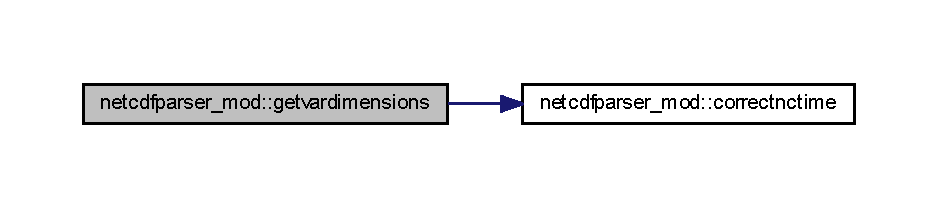
\includegraphics[width=350pt]{namespacenetcdfparser__mod_a0aea819b8a474ce2f4840d0bc44e95ec_cgraph}
\end{center}
\end{figure}
\mbox{\Hypertarget{namespacenetcdfparser__mod_ac01c000a97d23613684155708249ce89}\label{namespacenetcdfparser__mod_ac01c000a97d23613684155708249ce89}} 
\index{netcdfparser\+\_\+mod@{netcdfparser\+\_\+mod}!printdimsnc@{printdimsnc}}
\index{printdimsnc@{printdimsnc}!netcdfparser\+\_\+mod@{netcdfparser\+\_\+mod}}
\subsubsection{\texorpdfstring{printdimsnc()}{printdimsnc()}}
{\footnotesize\ttfamily subroutine netcdfparser\+\_\+mod\+::printdimsnc (\begin{DoxyParamCaption}\item[{class(\mbox{\hyperlink{structnetcdfparser__mod_1_1dim__t}{dim\+\_\+t}}), intent(inout)}]{self }\end{DoxyParamCaption})\hspace{0.3cm}{\ttfamily [private]}}



print dimensions metadata 

\begin{DoxyAuthor}{Author}
Ricardo Birjukovs Canelas -\/ M\+A\+R\+E\+T\+EC 
\end{DoxyAuthor}

\begin{DoxyParams}[1]{Parameters}
\mbox{\tt in}  & {\em self} & \\
\hline
\end{DoxyParams}


Definition at line 502 of file Net\+C\+D\+Fparser.\+f90.


\begin{DoxyCode}
502     \textcolor{keywordtype}{class}(dim\_t), \textcolor{keywordtype}{intent(inout)} :: self
503     \textcolor{keywordtype}{type}(string) :: outext, temp
504     outext = \textcolor{stringliteral}{'--->Dimension: '}// self%name //new\_line(\textcolor{stringliteral}{'a'})
505     temp = self%dimid
506     outext = outext//\textcolor{stringliteral}{'       dimid = '}//temp//new\_line(\textcolor{stringliteral}{'a'})
507     temp = self%varid
508     outext = outext//\textcolor{stringliteral}{'       varid = '}//temp//new\_line(\textcolor{stringliteral}{'a'})
509     outext = outext//\textcolor{stringliteral}{'       units = '}//self%units//new\_line(\textcolor{stringliteral}{'a'})
510     temp = self%length
511     outext = outext//\textcolor{stringliteral}{'       lenght = '}//temp
512     \textcolor{keyword}{call }log%put(outext,.false.)
\end{DoxyCode}
\mbox{\Hypertarget{namespacenetcdfparser__mod_aeb48d33c014bae21b2fceaaa70cbdc67}\label{namespacenetcdfparser__mod_aeb48d33c014bae21b2fceaaa70cbdc67}} 
\index{netcdfparser\+\_\+mod@{netcdfparser\+\_\+mod}!printncinfo@{printncinfo}}
\index{printncinfo@{printncinfo}!netcdfparser\+\_\+mod@{netcdfparser\+\_\+mod}}
\subsubsection{\texorpdfstring{printncinfo()}{printncinfo()}}
{\footnotesize\ttfamily subroutine netcdfparser\+\_\+mod\+::printncinfo (\begin{DoxyParamCaption}\item[{class(\mbox{\hyperlink{structnetcdfparser__mod_1_1ncfile__class}{ncfile\+\_\+class}}), intent(inout)}]{self }\end{DoxyParamCaption})\hspace{0.3cm}{\ttfamily [private]}}



prints most of the file model metadata 

\begin{DoxyAuthor}{Author}
Daniel Garaboa Paz -\/ U\+SC 
\end{DoxyAuthor}

\begin{DoxyParams}[1]{Parameters}
\mbox{\tt in}  & {\em self} & \\
\hline
\end{DoxyParams}


Definition at line 460 of file Net\+C\+D\+Fparser.\+f90.


\begin{DoxyCode}
460     \textcolor{keywordtype}{class}(ncfile\_class), \textcolor{keywordtype}{intent(inout)} :: self
461     \textcolor{keywordtype}{type}(string) :: outext, temp
462     outext = \textcolor{stringliteral}{'-->Reading NetCDF file '}//self%filename%chars()//new\_line(\textcolor{stringliteral}{'a'})
463     temp = self%ncid
464     outext = outext//\textcolor{stringliteral}{'       file ID = '}//temp//new\_line(\textcolor{stringliteral}{'a'})
465     temp = self%nDims
466     outext = outext//\textcolor{stringliteral}{'       Number of dimensions = '}//temp//new\_line(\textcolor{stringliteral}{'a'})
467     temp = self%nVars
468     outext = outext//\textcolor{stringliteral}{'       Number of variable fields = '}//temp
469     \textcolor{keyword}{call }log%put(outext,.false.)
\end{DoxyCode}
\mbox{\Hypertarget{namespacenetcdfparser__mod_a6b57fa47d7bd796c75483216a51e5e04}\label{namespacenetcdfparser__mod_a6b57fa47d7bd796c75483216a51e5e04}} 
\index{netcdfparser\+\_\+mod@{netcdfparser\+\_\+mod}!printvarsnc@{printvarsnc}}
\index{printvarsnc@{printvarsnc}!netcdfparser\+\_\+mod@{netcdfparser\+\_\+mod}}
\subsubsection{\texorpdfstring{printvarsnc()}{printvarsnc()}}
{\footnotesize\ttfamily subroutine netcdfparser\+\_\+mod\+::printvarsnc (\begin{DoxyParamCaption}\item[{class(\mbox{\hyperlink{structnetcdfparser__mod_1_1var__t}{var\+\_\+t}}), intent(inout)}]{self }\end{DoxyParamCaption})\hspace{0.3cm}{\ttfamily [private]}}



print variable metadata 

\begin{DoxyAuthor}{Author}
Ricardo Birjukovs Canelas -\/ M\+A\+R\+E\+T\+EC 
\end{DoxyAuthor}

\begin{DoxyParams}[1]{Parameters}
\mbox{\tt in}  & {\em self} & \\
\hline
\end{DoxyParams}


Definition at line 479 of file Net\+C\+D\+Fparser.\+f90.


\begin{DoxyCode}
479     \textcolor{keywordtype}{class}(var\_t), \textcolor{keywordtype}{intent(inout)} :: self
480     \textcolor{keywordtype}{type}(string) :: outext, temp
481     \textcolor{keywordtype}{integer} :: i
482     outext = \textcolor{stringliteral}{'--->Variable: '}// self%name //new\_line(\textcolor{stringliteral}{'a'})
483     temp = self%varid
484     outext = outext//\textcolor{stringliteral}{'       varid = '}//temp//new\_line(\textcolor{stringliteral}{'a'})
485     outext = outext//\textcolor{stringliteral}{'       units = '}//self%units//new\_line(\textcolor{stringliteral}{'a'})
486     temp = self%dimids(1)
487     outext = outext//\textcolor{stringliteral}{'       dimids = '}//temp
488     \textcolor{keywordflow}{do} i=2, \textcolor{keyword}{size}(self%dimids)
489         temp = self%dimids(i)
490         outext = outext//\textcolor{stringliteral}{', '}//temp
491 \textcolor{keywordflow}{    end do}
492     \textcolor{keyword}{call }log%put(outext,.false.)
\end{DoxyCode}

\hypertarget{namespacesimulation__mod}{}\section{simulation\+\_\+mod Module Reference}
\label{namespacesimulation__mod}\index{simulation\+\_\+mod@{simulation\+\_\+mod}}


Module to hold the simulation class and its methods. This is the only class that is exposed to an external program, as it encapsulates every other class and method.  


\subsection*{Data Types}
\begin{DoxyCompactItemize}
\item 
type \mbox{\hyperlink{structsimulation__mod_1_1simulation__class}{simulation\+\_\+class}}
\end{DoxyCompactItemize}
\subsection*{Functions/\+Subroutines}
\begin{DoxyCompactItemize}
\item 
subroutine \mbox{\hyperlink{namespacesimulation__mod_a73bd78c4ac76c51f1e10f5847c25c4df}{run}} (self)
\begin{DoxyCompactList}\small\item\em Simulation run method. Runs the initialized case main time cycle. \end{DoxyCompactList}\item 
subroutine \mbox{\hyperlink{namespacesimulation__mod_aedbba2bb458cbcd7eb93938a5f7b5940}{initsimulation}} (self, casefilename, outpath)
\begin{DoxyCompactList}\small\item\em Simulation initialization method. Effectively builds and populates the simulation objects that will be used latter on. \end{DoxyCompactList}\item 
subroutine \mbox{\hyperlink{namespacesimulation__mod_a87a5141e4516b9610a6e4f0d2ff2d719}{togglesources}} (self)
\begin{DoxyCompactList}\small\item\em Simulation method to activate and deactivate Sources based on the GlobalSim\+Time. \end{DoxyCompactList}\item 
subroutine \mbox{\hyperlink{namespacesimulation__mod_a13aa0745f4601e3f418143dab2f18276}{blocksemitt}} (self)
\begin{DoxyCompactList}\small\item\em Simulation method to call the Blocks to emitt tracers at current Sim\+Time. \end{DoxyCompactList}\item 
subroutine \mbox{\hyperlink{namespacesimulation__mod_a058892630af07fc0fe8a4bffec531c6a}{blocksdistribute}} (self)
\begin{DoxyCompactList}\small\item\em Simulation method to call the Blocks to distribute Tracers at current Sim\+Time. \end{DoxyCompactList}\item 
subroutine \mbox{\hyperlink{namespacesimulation__mod_ac838d4afe33303dc49a5790ca957baa1}{blocksconsolidatearrays}} (self)
\begin{DoxyCompactList}\small\item\em Simulation method to call the Blocks to consolidate the Tracer array at current Sim\+Time. \end{DoxyCompactList}\item 
subroutine \mbox{\hyperlink{namespacesimulation__mod_a624d5b402a8d359219839841862ab307}{blockstracerstoaot}} (self)
\begin{DoxyCompactList}\small\item\em Simulation method to call the Blocks to build their Array of Tracers (AoT) from the Tracer list at current Sim\+Time. \end{DoxyCompactList}\item 
subroutine \mbox{\hyperlink{namespacesimulation__mod_a03afd8682d3239c0ce8eb1637e4da806}{blocksaottotracers}} (self)
\begin{DoxyCompactList}\small\item\em Simulation method to call the Blocks to print their Array of Tracers (AoT) back to the Tracer objects on the list at current Sim\+Time. \end{DoxyCompactList}\item 
subroutine \mbox{\hyperlink{namespacesimulation__mod_a9c7e093e5cf65d3414f9a8cf8beab611}{blockscleanaot}} (self)
\begin{DoxyCompactList}\small\item\em Simulation method to call the Blocks to clean their Array of Tracers (AoT) at current Sim\+Time. \end{DoxyCompactList}\item 
subroutine \mbox{\hyperlink{namespacesimulation__mod_a447c6d709de6aa360a65d39d660e627b}{setinitialstate}} (self)
\begin{DoxyCompactList}\small\item\em Simulation method to distribute the Sources to the Blocks, allocate the respective Tracers and redistribute if needed. \end{DoxyCompactList}\item 
integer function \mbox{\hyperlink{namespacesimulation__mod_a0ad485eab624ffa4df282f1da8d9f214}{gettracertotals}} (self)
\begin{DoxyCompactList}\small\item\em Simulation method to count Tracer numbers. \end{DoxyCompactList}\item 
subroutine \mbox{\hyperlink{namespacesimulation__mod_aba126a8e0575cabb3bef6ab395002b3c}{printtracertotals}} (self)
\begin{DoxyCompactList}\small\item\em Simulation method to count Tracer numbers. \end{DoxyCompactList}\item 
subroutine \mbox{\hyperlink{namespacesimulation__mod_acc5fa823c8dd599de8feda8988c224f2}{settracermemory}} (self, ntrc)
\begin{DoxyCompactList}\small\item\em Simulation method to account for Tracer memory consumption. \end{DoxyCompactList}\item 
subroutine \mbox{\hyperlink{namespacesimulation__mod_a2b8198a9fb3f7671c6b45192a0b9740c}{decomposedomain}} (self)
\begin{DoxyCompactList}\small\item\em Simulation method to do domain decomposition and define the Blocks. \end{DoxyCompactList}\item 
subroutine \mbox{\hyperlink{namespacesimulation__mod_a4285722eaa589fa671233554b54c74f8}{closesimulation}} (self)
\begin{DoxyCompactList}\small\item\em Simulation finishing method. Closes output files and writes the final messages. \end{DoxyCompactList}\end{DoxyCompactItemize}


\subsection{Detailed Description}
Module to hold the simulation class and its methods. This is the only class that is exposed to an external program, as it encapsulates every other class and method. 

\begin{DoxyAuthor}{Author}
Ricardo Birjukovs Canelas 
\end{DoxyAuthor}


\subsection{Function/\+Subroutine Documentation}
\mbox{\Hypertarget{namespacesimulation__mod_a03afd8682d3239c0ce8eb1637e4da806}\label{namespacesimulation__mod_a03afd8682d3239c0ce8eb1637e4da806}} 
\index{simulation\+\_\+mod@{simulation\+\_\+mod}!blocksaottotracers@{blocksaottotracers}}
\index{blocksaottotracers@{blocksaottotracers}!simulation\+\_\+mod@{simulation\+\_\+mod}}
\subsubsection{\texorpdfstring{blocksaottotracers()}{blocksaottotracers()}}
{\footnotesize\ttfamily subroutine simulation\+\_\+mod\+::blocksaottotracers (\begin{DoxyParamCaption}\item[{class(\mbox{\hyperlink{structsimulation__mod_1_1simulation__class}{simulation\+\_\+class}}), intent(in)}]{self }\end{DoxyParamCaption})\hspace{0.3cm}{\ttfamily [private]}}



Simulation method to call the Blocks to print their Array of Tracers (AoT) back to the Tracer objects on the list at current Sim\+Time. 

\begin{DoxyAuthor}{Author}
Ricardo Birjukovs Canelas -\/ M\+A\+R\+E\+T\+EC 
\end{DoxyAuthor}


Definition at line 251 of file simulation.\+f90.


\begin{DoxyCode}
251     \textcolor{keywordtype}{implicit none}
252     \textcolor{keywordtype}{class}(simulation\_class), \textcolor{keywordtype}{intent(in)} :: self
253     \textcolor{keywordtype}{integer} :: i
254     \textcolor{keywordflow}{do} i=1, \textcolor{keyword}{size}(dblock)
255         \textcolor{keyword}{call }dblock(i)%AoTtoTracers()
256 \textcolor{keywordflow}{    enddo}
\end{DoxyCode}
\mbox{\Hypertarget{namespacesimulation__mod_a9c7e093e5cf65d3414f9a8cf8beab611}\label{namespacesimulation__mod_a9c7e093e5cf65d3414f9a8cf8beab611}} 
\index{simulation\+\_\+mod@{simulation\+\_\+mod}!blockscleanaot@{blockscleanaot}}
\index{blockscleanaot@{blockscleanaot}!simulation\+\_\+mod@{simulation\+\_\+mod}}
\subsubsection{\texorpdfstring{blockscleanaot()}{blockscleanaot()}}
{\footnotesize\ttfamily subroutine simulation\+\_\+mod\+::blockscleanaot (\begin{DoxyParamCaption}\item[{class(\mbox{\hyperlink{structsimulation__mod_1_1simulation__class}{simulation\+\_\+class}}), intent(in)}]{self }\end{DoxyParamCaption})\hspace{0.3cm}{\ttfamily [private]}}



Simulation method to call the Blocks to clean their Array of Tracers (AoT) at current Sim\+Time. 

\begin{DoxyAuthor}{Author}
Ricardo Birjukovs Canelas -\/ M\+A\+R\+E\+T\+EC 
\end{DoxyAuthor}


Definition at line 266 of file simulation.\+f90.


\begin{DoxyCode}
266     \textcolor{keywordtype}{implicit none}
267     \textcolor{keywordtype}{class}(simulation\_class), \textcolor{keywordtype}{intent(in)} :: self
268     \textcolor{keywordtype}{integer} :: i
269     \textcolor{keywordflow}{do} i=1, \textcolor{keyword}{size}(dblock)
270         \textcolor{keyword}{call }dblock(i)%CleanAoT()
271 \textcolor{keywordflow}{    enddo}
\end{DoxyCode}
\mbox{\Hypertarget{namespacesimulation__mod_ac838d4afe33303dc49a5790ca957baa1}\label{namespacesimulation__mod_ac838d4afe33303dc49a5790ca957baa1}} 
\index{simulation\+\_\+mod@{simulation\+\_\+mod}!blocksconsolidatearrays@{blocksconsolidatearrays}}
\index{blocksconsolidatearrays@{blocksconsolidatearrays}!simulation\+\_\+mod@{simulation\+\_\+mod}}
\subsubsection{\texorpdfstring{blocksconsolidatearrays()}{blocksconsolidatearrays()}}
{\footnotesize\ttfamily subroutine simulation\+\_\+mod\+::blocksconsolidatearrays (\begin{DoxyParamCaption}\item[{class(\mbox{\hyperlink{structsimulation__mod_1_1simulation__class}{simulation\+\_\+class}}), intent(in)}]{self }\end{DoxyParamCaption})\hspace{0.3cm}{\ttfamily [private]}}



Simulation method to call the Blocks to consolidate the Tracer array at current Sim\+Time. 

\begin{DoxyAuthor}{Author}
Ricardo Birjukovs Canelas -\/ M\+A\+R\+E\+T\+EC 
\end{DoxyAuthor}


Definition at line 221 of file simulation.\+f90.


\begin{DoxyCode}
221     \textcolor{keywordtype}{implicit none}
222     \textcolor{keywordtype}{class}(simulation\_class), \textcolor{keywordtype}{intent(in)} :: self
223     \textcolor{keywordtype}{integer} :: i
224     \textcolor{keywordflow}{do} i=1, \textcolor{keyword}{size}(dblock)
225         \textcolor{keyword}{call }dblock(i)%ConsolidateArrays()
226 \textcolor{keywordflow}{    enddo}
\end{DoxyCode}
\mbox{\Hypertarget{namespacesimulation__mod_a058892630af07fc0fe8a4bffec531c6a}\label{namespacesimulation__mod_a058892630af07fc0fe8a4bffec531c6a}} 
\index{simulation\+\_\+mod@{simulation\+\_\+mod}!blocksdistribute@{blocksdistribute}}
\index{blocksdistribute@{blocksdistribute}!simulation\+\_\+mod@{simulation\+\_\+mod}}
\subsubsection{\texorpdfstring{blocksdistribute()}{blocksdistribute()}}
{\footnotesize\ttfamily subroutine simulation\+\_\+mod\+::blocksdistribute (\begin{DoxyParamCaption}\item[{class(\mbox{\hyperlink{structsimulation__mod_1_1simulation__class}{simulation\+\_\+class}}), intent(in)}]{self }\end{DoxyParamCaption})\hspace{0.3cm}{\ttfamily [private]}}



Simulation method to call the Blocks to distribute Tracers at current Sim\+Time. 

\begin{DoxyAuthor}{Author}
Ricardo Birjukovs Canelas -\/ M\+A\+R\+E\+T\+EC 
\end{DoxyAuthor}


Definition at line 205 of file simulation.\+f90.


\begin{DoxyCode}
205     \textcolor{keywordtype}{implicit none}
206     \textcolor{keywordtype}{class}(simulation\_class), \textcolor{keywordtype}{intent(in)} :: self
207     \textcolor{keywordtype}{integer} :: i
208     \textcolor{keywordflow}{do} i=1, \textcolor{keyword}{size}(dblock)
209         \textcolor{keyword}{call }dblock(i)%DistributeTracers()
210 \textcolor{keywordflow}{    enddo}
211     \textcolor{comment}{!need to distribute Sources also! TODO}
\end{DoxyCode}
\mbox{\Hypertarget{namespacesimulation__mod_a13aa0745f4601e3f418143dab2f18276}\label{namespacesimulation__mod_a13aa0745f4601e3f418143dab2f18276}} 
\index{simulation\+\_\+mod@{simulation\+\_\+mod}!blocksemitt@{blocksemitt}}
\index{blocksemitt@{blocksemitt}!simulation\+\_\+mod@{simulation\+\_\+mod}}
\subsubsection{\texorpdfstring{blocksemitt()}{blocksemitt()}}
{\footnotesize\ttfamily subroutine simulation\+\_\+mod\+::blocksemitt (\begin{DoxyParamCaption}\item[{class(\mbox{\hyperlink{structsimulation__mod_1_1simulation__class}{simulation\+\_\+class}}), intent(in)}]{self }\end{DoxyParamCaption})\hspace{0.3cm}{\ttfamily [private]}}



Simulation method to call the Blocks to emitt tracers at current Sim\+Time. 

\begin{DoxyAuthor}{Author}
Ricardo Birjukovs Canelas -\/ M\+A\+R\+E\+T\+EC 
\end{DoxyAuthor}


Definition at line 190 of file simulation.\+f90.


\begin{DoxyCode}
190     \textcolor{keywordtype}{implicit none}
191     \textcolor{keywordtype}{class}(simulation\_class), \textcolor{keywordtype}{intent(in)} :: self
192     \textcolor{keywordtype}{integer} :: i
193     \textcolor{keywordflow}{do} i=1, \textcolor{keyword}{size}(dblock)
194         \textcolor{keyword}{call }dblock(i)%CallEmitter()
195 \textcolor{keywordflow}{    enddo}
\end{DoxyCode}
\mbox{\Hypertarget{namespacesimulation__mod_a624d5b402a8d359219839841862ab307}\label{namespacesimulation__mod_a624d5b402a8d359219839841862ab307}} 
\index{simulation\+\_\+mod@{simulation\+\_\+mod}!blockstracerstoaot@{blockstracerstoaot}}
\index{blockstracerstoaot@{blockstracerstoaot}!simulation\+\_\+mod@{simulation\+\_\+mod}}
\subsubsection{\texorpdfstring{blockstracerstoaot()}{blockstracerstoaot()}}
{\footnotesize\ttfamily subroutine simulation\+\_\+mod\+::blockstracerstoaot (\begin{DoxyParamCaption}\item[{class(\mbox{\hyperlink{structsimulation__mod_1_1simulation__class}{simulation\+\_\+class}}), intent(in)}]{self }\end{DoxyParamCaption})\hspace{0.3cm}{\ttfamily [private]}}



Simulation method to call the Blocks to build their Array of Tracers (AoT) from the Tracer list at current Sim\+Time. 

\begin{DoxyAuthor}{Author}
Ricardo Birjukovs Canelas -\/ M\+A\+R\+E\+T\+EC 
\end{DoxyAuthor}


Definition at line 236 of file simulation.\+f90.


\begin{DoxyCode}
236     \textcolor{keywordtype}{implicit none}
237     \textcolor{keywordtype}{class}(simulation\_class), \textcolor{keywordtype}{intent(in)} :: self
238     \textcolor{keywordtype}{integer} :: i
239     \textcolor{keywordflow}{do} i=1, \textcolor{keyword}{size}(dblock)
240         \textcolor{keyword}{call }dblock(i)%TracersToAoT()
241 \textcolor{keywordflow}{    enddo}
\end{DoxyCode}
\mbox{\Hypertarget{namespacesimulation__mod_a4285722eaa589fa671233554b54c74f8}\label{namespacesimulation__mod_a4285722eaa589fa671233554b54c74f8}} 
\index{simulation\+\_\+mod@{simulation\+\_\+mod}!closesimulation@{closesimulation}}
\index{closesimulation@{closesimulation}!simulation\+\_\+mod@{simulation\+\_\+mod}}
\subsubsection{\texorpdfstring{closesimulation()}{closesimulation()}}
{\footnotesize\ttfamily subroutine simulation\+\_\+mod\+::closesimulation (\begin{DoxyParamCaption}\item[{class(\mbox{\hyperlink{structsimulation__mod_1_1simulation__class}{simulation\+\_\+class}}), intent(inout)}]{self }\end{DoxyParamCaption})\hspace{0.3cm}{\ttfamily [private]}}



Simulation finishing method. Closes output files and writes the final messages. 

\begin{DoxyAuthor}{Author}
Ricardo Birjukovs Canelas -\/ M\+A\+R\+E\+T\+EC 
\end{DoxyAuthor}


Definition at line 379 of file simulation.\+f90.


\begin{DoxyCode}
379     \textcolor{keywordtype}{implicit none}
380     \textcolor{keywordtype}{class}(simulation\_class), \textcolor{keywordtype}{intent(inout)} :: self
381     \textcolor{keywordtype}{type}(string) :: outext
382     outext=\textcolor{stringliteral}{'Simulation ended, freeing resources. See you next time'}
383     \textcolor{keyword}{call }log%put(outext)
384     \textcolor{keyword}{call }log%finalize()
\end{DoxyCode}
\mbox{\Hypertarget{namespacesimulation__mod_a2b8198a9fb3f7671c6b45192a0b9740c}\label{namespacesimulation__mod_a2b8198a9fb3f7671c6b45192a0b9740c}} 
\index{simulation\+\_\+mod@{simulation\+\_\+mod}!decomposedomain@{decomposedomain}}
\index{decomposedomain@{decomposedomain}!simulation\+\_\+mod@{simulation\+\_\+mod}}
\subsubsection{\texorpdfstring{decomposedomain()}{decomposedomain()}}
{\footnotesize\ttfamily subroutine simulation\+\_\+mod\+::decomposedomain (\begin{DoxyParamCaption}\item[{class(\mbox{\hyperlink{structsimulation__mod_1_1simulation__class}{simulation\+\_\+class}}), intent(inout)}]{self }\end{DoxyParamCaption})\hspace{0.3cm}{\ttfamily [private]}}



Simulation method to do domain decomposition and define the Blocks. 

\begin{DoxyAuthor}{Author}
Ricardo Birjukovs Canelas -\/ M\+A\+R\+E\+T\+EC 
\end{DoxyAuthor}


Definition at line 359 of file simulation.\+f90.


\begin{DoxyCode}
359     \textcolor{keywordtype}{implicit none}
360     \textcolor{keywordtype}{class}(simulation\_class), \textcolor{keywordtype}{intent(inout)} :: self
361     \textcolor{keywordtype}{type}(string) :: outext
362     \textcolor{keywordflow}{if} (globals%SimDefs%autoblocksize) \textcolor{keywordflow}{then}
363         \textcolor{keyword}{call }allocblocks(globals%SimDefs%numblocks)
364     \textcolor{keywordflow}{else}
365         outext=\textcolor{stringliteral}{'[DecomposeDomain]: Only automatic Block sizing at the moment, stoping'}
366         \textcolor{keyword}{call }log%put(outext)
367         stop
368 \textcolor{keywordflow}{    end if}
369     \textcolor{comment}{! Initializing the Blocks}
370     \textcolor{keyword}{call }setblocks(globals%SimDefs%autoblocksize,globals%SimDefs%numblocks,globals%SimDefs%numblocksx,
      globals%SimDefs%numblocksy)
\end{DoxyCode}
Here is the call graph for this function\+:\nopagebreak
\begin{figure}[H]
\begin{center}
\leavevmode
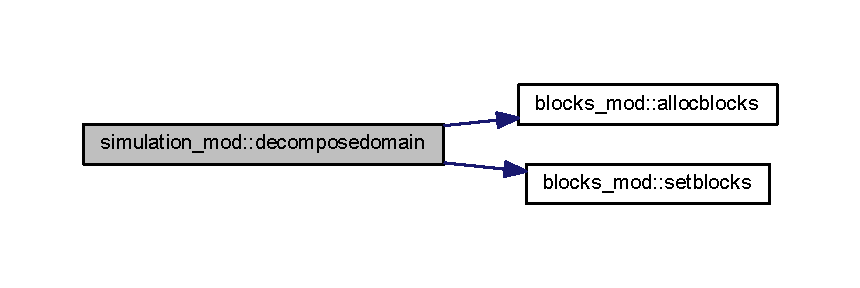
\includegraphics[width=350pt]{namespacesimulation__mod_a2b8198a9fb3f7671c6b45192a0b9740c_cgraph}
\end{center}
\end{figure}
\mbox{\Hypertarget{namespacesimulation__mod_a0ad485eab624ffa4df282f1da8d9f214}\label{namespacesimulation__mod_a0ad485eab624ffa4df282f1da8d9f214}} 
\index{simulation\+\_\+mod@{simulation\+\_\+mod}!gettracertotals@{gettracertotals}}
\index{gettracertotals@{gettracertotals}!simulation\+\_\+mod@{simulation\+\_\+mod}}
\subsubsection{\texorpdfstring{gettracertotals()}{gettracertotals()}}
{\footnotesize\ttfamily integer function simulation\+\_\+mod\+::gettracertotals (\begin{DoxyParamCaption}\item[{class(\mbox{\hyperlink{structsimulation__mod_1_1simulation__class}{simulation\+\_\+class}}), intent(in)}]{self }\end{DoxyParamCaption})\hspace{0.3cm}{\ttfamily [private]}}



Simulation method to count Tracer numbers. 

\begin{DoxyAuthor}{Author}
Ricardo Birjukovs Canelas -\/ M\+A\+R\+E\+T\+EC 
\end{DoxyAuthor}


Definition at line 307 of file simulation.\+f90.


\begin{DoxyCode}
307     \textcolor{keywordtype}{implicit none}
308     \textcolor{keywordtype}{class}(simulation\_class), \textcolor{keywordtype}{intent(in)} :: self
309     \textcolor{keywordtype}{integer} :: i, total
310     total = 0
311     \textcolor{keywordflow}{do} i=1, \textcolor{keyword}{size}(dblock)
312         total = total + dblock(i)%numAllocTracers()
313 \textcolor{keywordflow}{    enddo}
314     gettracertotals = total
\end{DoxyCode}
\mbox{\Hypertarget{namespacesimulation__mod_aedbba2bb458cbcd7eb93938a5f7b5940}\label{namespacesimulation__mod_aedbba2bb458cbcd7eb93938a5f7b5940}} 
\index{simulation\+\_\+mod@{simulation\+\_\+mod}!initsimulation@{initsimulation}}
\index{initsimulation@{initsimulation}!simulation\+\_\+mod@{simulation\+\_\+mod}}
\subsubsection{\texorpdfstring{initsimulation()}{initsimulation()}}
{\footnotesize\ttfamily subroutine simulation\+\_\+mod\+::initsimulation (\begin{DoxyParamCaption}\item[{class(\mbox{\hyperlink{structsimulation__mod_1_1simulation__class}{simulation\+\_\+class}}), intent(inout)}]{self,  }\item[{type(string), intent(in)}]{casefilename,  }\item[{type(string), intent(in)}]{outpath }\end{DoxyParamCaption})\hspace{0.3cm}{\ttfamily [private]}}



Simulation initialization method. Effectively builds and populates the simulation objects that will be used latter on. 

\begin{DoxyAuthor}{Author}
Ricardo Birjukovs Canelas -\/ M\+A\+R\+E\+T\+EC 
\end{DoxyAuthor}

\begin{DoxyParams}[1]{Parameters}
\mbox{\tt in}  & {\em self,casefilename,outpath} & \\
\hline
\mbox{\tt in}  & {\em casefilename} & case file name\\
\hline
\mbox{\tt in}  & {\em outpath} & Output path \\
\hline
\end{DoxyParams}


Definition at line 123 of file simulation.\+f90.


\begin{DoxyCode}
123     \textcolor{keywordtype}{implicit none}
124     \textcolor{keywordtype}{class}(simulation\_class), \textcolor{keywordtype}{intent(inout)} :: self
125     \textcolor{keywordtype}{type}(string), \textcolor{keywordtype}{intent(in)} :: casefilename
126     \textcolor{keywordtype}{type}(string), \textcolor{keywordtype}{intent(in)} :: outpath
127     \textcolor{keywordtype}{type}(string) :: outext
128     \textcolor{comment}{!type(generic\_field\_class) :: testField}
129     \textcolor{comment}{!type(background\_class) :: testBackground}
130 
131     \textcolor{comment}{! Initialize logger}
132     \textcolor{keyword}{call }log%initialize(outpath)
133     \textcolor{comment}{!Print licences and build info}
134     \textcolor{keyword}{call }printlicpreamble
135     \textcolor{comment}{!initializing memory log}
136     \textcolor{keyword}{call }simmemory%initialize()
137     \textcolor{comment}{!setting every global variable and input parameter to their default}
138     \textcolor{keyword}{call }globals%initialize(outpath = outpath)
139     \textcolor{comment}{!initializing geometry class}
140     \textcolor{keyword}{call }geometry%initialize()
141     \textcolor{comment}{!Check if case file has .xml extension}
142     \textcolor{keywordflow}{if} (casefilename%extension() == \textcolor{stringliteral}{'.xml'}) \textcolor{keywordflow}{then}
143         \textcolor{comment}{! Initialization routines to build the simulation from the input case file}
144         \textcolor{keyword}{call }initfromxml(casefilename)
145     \textcolor{keywordflow}{else}
146         outext=\textcolor{stringliteral}{'[initSimulation]: only .xml input files are supported at the time. Stopping'}
147         \textcolor{keyword}{call }log%put(outext)
148         stop
149 \textcolor{keywordflow}{    endif}
150     \textcolor{comment}{!Case was read and now we can build/initialize our simulation objects that are case-dependent}
151     \textcolor{comment}{!initilize simulation bounding box}
152     \textcolor{keyword}{call }bbox%initialize()
153     \textcolor{comment}{!decomposing the domain and initializing the Simulation Blocks}
154     \textcolor{keyword}{call }self%decompose()
155     \textcolor{comment}{!Distributing Sources}
156     \textcolor{keyword}{call }self%setInitialState()
157     \textcolor{comment}{!printing memory occupation at the time}
158     \textcolor{keyword}{call }simmemory%detailedprint()
159     \textcolor{comment}{!Initializing output file streamer}
160     \textcolor{keyword}{call }outputstreamer%initialize()
161     \textcolor{comment}{!Writing the domain to file}
162     \textcolor{keyword}{call }outputstreamer%WriteDomain(globals%Names%casename, bbox, geometry%getnumPoints(bbox), dblock)
163 
164     \textcolor{comment}{!call testField%test()}
165     \textcolor{comment}{!call testBackground%test()}
166 
\end{DoxyCode}
Here is the call graph for this function\+:\nopagebreak
\begin{figure}[H]
\begin{center}
\leavevmode
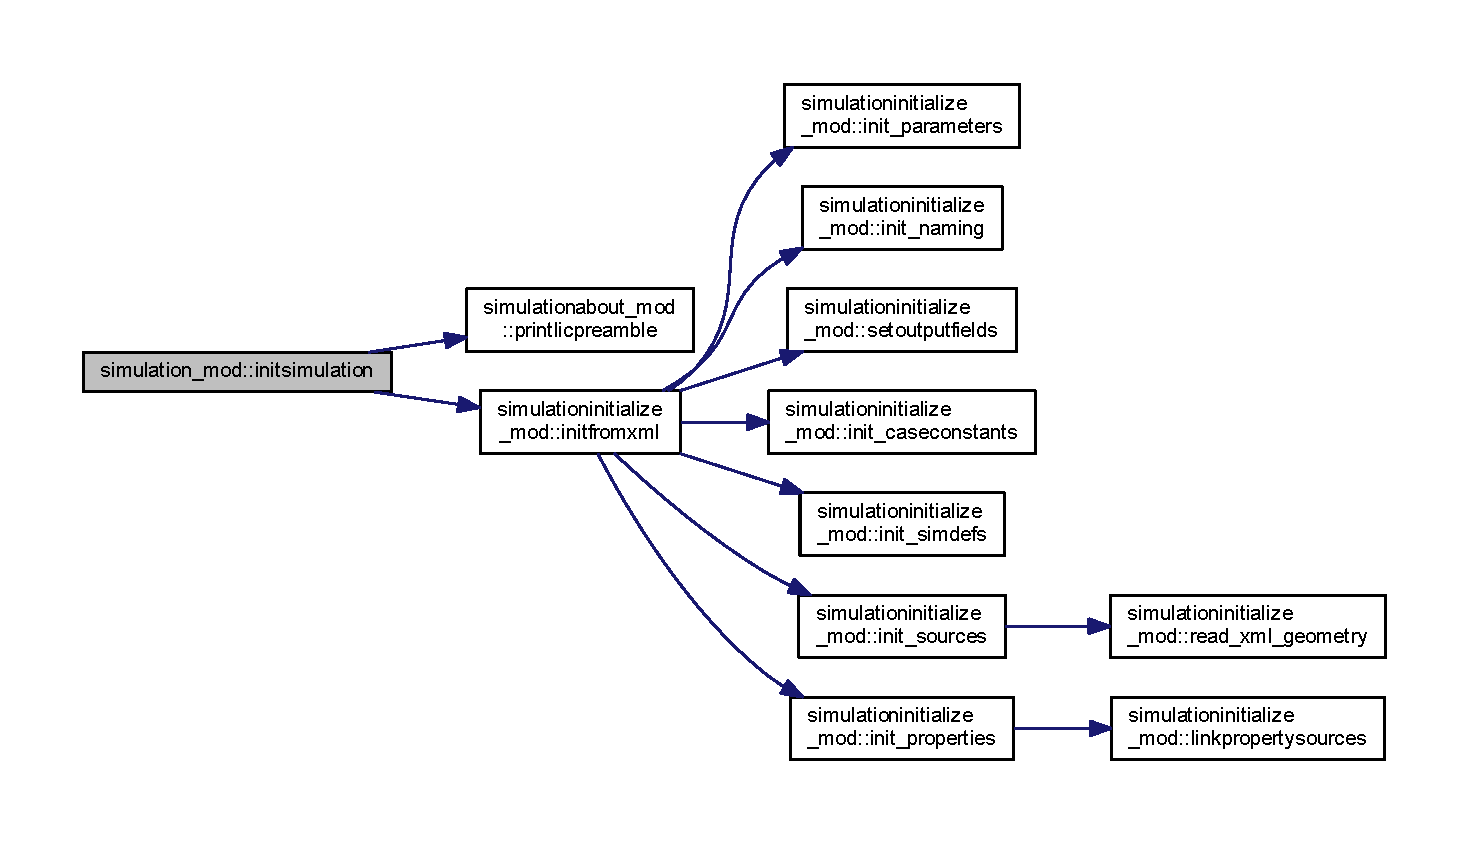
\includegraphics[width=350pt]{namespacesimulation__mod_aedbba2bb458cbcd7eb93938a5f7b5940_cgraph}
\end{center}
\end{figure}
\mbox{\Hypertarget{namespacesimulation__mod_aba126a8e0575cabb3bef6ab395002b3c}\label{namespacesimulation__mod_aba126a8e0575cabb3bef6ab395002b3c}} 
\index{simulation\+\_\+mod@{simulation\+\_\+mod}!printtracertotals@{printtracertotals}}
\index{printtracertotals@{printtracertotals}!simulation\+\_\+mod@{simulation\+\_\+mod}}
\subsubsection{\texorpdfstring{printtracertotals()}{printtracertotals()}}
{\footnotesize\ttfamily subroutine simulation\+\_\+mod\+::printtracertotals (\begin{DoxyParamCaption}\item[{class(\mbox{\hyperlink{structsimulation__mod_1_1simulation__class}{simulation\+\_\+class}}), intent(in)}]{self }\end{DoxyParamCaption})\hspace{0.3cm}{\ttfamily [private]}}



Simulation method to count Tracer numbers. 

\begin{DoxyAuthor}{Author}
Ricardo Birjukovs Canelas -\/ M\+A\+R\+E\+T\+EC 
\end{DoxyAuthor}


Definition at line 323 of file simulation.\+f90.


\begin{DoxyCode}
323     \textcolor{keywordtype}{implicit none}
324     \textcolor{keywordtype}{class}(simulation\_class), \textcolor{keywordtype}{intent(in)} :: self
325     \textcolor{keywordtype}{type}(string) :: outext, temp
326     temp = self%getTracerTotals()
327     outext=\textcolor{stringliteral}{'-->'}//temp //\textcolor{stringliteral}{' Tracers allocated'}
328     \textcolor{keyword}{call }log%put(outext,.false.)
\end{DoxyCode}
\mbox{\Hypertarget{namespacesimulation__mod_a73bd78c4ac76c51f1e10f5847c25c4df}\label{namespacesimulation__mod_a73bd78c4ac76c51f1e10f5847c25c4df}} 
\index{simulation\+\_\+mod@{simulation\+\_\+mod}!run@{run}}
\index{run@{run}!simulation\+\_\+mod@{simulation\+\_\+mod}}
\subsubsection{\texorpdfstring{run()}{run()}}
{\footnotesize\ttfamily subroutine simulation\+\_\+mod\+::run (\begin{DoxyParamCaption}\item[{class(\mbox{\hyperlink{structsimulation__mod_1_1simulation__class}{simulation\+\_\+class}}), intent(inout)}]{self }\end{DoxyParamCaption})\hspace{0.3cm}{\ttfamily [private]}}



Simulation run method. Runs the initialized case main time cycle. 

\begin{DoxyAuthor}{Author}
Ricardo Birjukovs Canelas -\/ M\+A\+R\+E\+T\+EC 
\end{DoxyAuthor}


Definition at line 68 of file simulation.\+f90.


\begin{DoxyCode}
68     \textcolor{keywordtype}{implicit none}
69     \textcolor{keywordtype}{class}(simulation\_class), \textcolor{keywordtype}{intent(inout)} :: self
70     \textcolor{keywordtype}{type}(string) :: outext
71 
72     outext = \textcolor{stringliteral}{'====================================================================='}
73     \textcolor{keyword}{call }log%put(outext,.false.)
74     outext = \textcolor{stringliteral}{'->Simulation starting'}
75     \textcolor{keyword}{call }log%put(outext)
76     outext = \textcolor{stringliteral}{'====================================================================='}
77     \textcolor{keyword}{call }log%put(outext,.false.)
78 
79     \textcolor{comment}{!main time cycle}
80     \textcolor{keywordflow}{do} \textcolor{keywordflow}{while} (globals%SimTime .lt. globals%Parameters%TimeMax)
81         \textcolor{comment}{!activate suitable Sources}
82         \textcolor{keyword}{call }self%ToggleSources()
83         \textcolor{comment}{!emitt Tracers from active Sources}
84         \textcolor{keyword}{call }self%BlocksEmitt()
85         \textcolor{comment}{!Distribute Tracers and Sources by Blocks}
86         \textcolor{keyword}{call }self%BlocksDistribute()
87         \textcolor{comment}{!Optimize Block Tracer lists}
88         \textcolor{keyword}{call }self%BlocksConsolidateArrays()
89         \textcolor{comment}{!Build AoT}
90         \textcolor{keyword}{call }self%BlocksTracersToAoT()
91         \textcolor{comment}{!load hydrodynamic fields from files (curents, wind, waves, ...)}
92         \textcolor{comment}{!Update all tracers with base behavior (AoT) - Integration step}
93         \textcolor{comment}{!interpolate fields to tracer coordinates}
94         \textcolor{comment}{!AoT to Tracers}
95         \textcolor{keyword}{call }self%BlocksAoTtoTracers()
96         \textcolor{comment}{!Update Tracers with type-specific behavior}
97         \textcolor{comment}{!Write results if time to do so}
98         \textcolor{keyword}{call }outputstreamer%WriteStepSerial(dblock)
99         \textcolor{comment}{!Print some stats from the time step}
100         \textcolor{keyword}{call }self%printTracerTotals()
101         \textcolor{comment}{!Clean AoT}
102         \textcolor{keyword}{call }self%BlocksCleanAoT()
103         \textcolor{comment}{!update Simulation time and counters}
104         globals%SimTime = globals%SimTime + globals%SimDefs%dt
105         \textcolor{keyword}{call }globals%Sim%increment\_numdt()
106         \textcolor{comment}{!print*, 'Global time is ', Globals%SimTime}
107         \textcolor{comment}{!print*, 'Can we continue?'}
108         \textcolor{comment}{!read (*,*)}
109 \textcolor{keywordflow}{    enddo}
110     \textcolor{keyword}{call }self%setTracerMemory()
111     \textcolor{keyword}{call }simmemory%detailedprint()
112 
\end{DoxyCode}
\mbox{\Hypertarget{namespacesimulation__mod_a447c6d709de6aa360a65d39d660e627b}\label{namespacesimulation__mod_a447c6d709de6aa360a65d39d660e627b}} 
\index{simulation\+\_\+mod@{simulation\+\_\+mod}!setinitialstate@{setinitialstate}}
\index{setinitialstate@{setinitialstate}!simulation\+\_\+mod@{simulation\+\_\+mod}}
\subsubsection{\texorpdfstring{setinitialstate()}{setinitialstate()}}
{\footnotesize\ttfamily subroutine simulation\+\_\+mod\+::setinitialstate (\begin{DoxyParamCaption}\item[{class(\mbox{\hyperlink{structsimulation__mod_1_1simulation__class}{simulation\+\_\+class}}), intent(inout)}]{self }\end{DoxyParamCaption})\hspace{0.3cm}{\ttfamily [private]}}



Simulation method to distribute the Sources to the Blocks, allocate the respective Tracers and redistribute if needed. 

\begin{DoxyAuthor}{Author}
Ricardo Birjukovs Canelas -\/ M\+A\+R\+E\+T\+EC 
\end{DoxyAuthor}


Definition at line 281 of file simulation.\+f90.


\begin{DoxyCode}
281     \textcolor{keywordtype}{implicit none}
282     \textcolor{keywordtype}{class}(simulation\_class), \textcolor{keywordtype}{intent(inout)} :: self
283     \textcolor{keywordtype}{type}(string) :: outext
284     \textcolor{keywordtype}{integer} :: i, blk, ntrc
285     \textcolor{comment}{!iterate every Source to distribute}
286     ntrc = 0
287     \textcolor{keywordflow}{do} i=1, \textcolor{keyword}{size}(tempsources%src)
288         blk = getblockindex(geometry%getCenter(tempsources%src(i)%par%geometry))
289         \textcolor{keyword}{call }dblock(blk)%putSource(tempsources%src(i))
290         ntrc = ntrc + tempsources%src(i)%stencil%total\_np
291 \textcolor{keywordflow}{    end do}
292     \textcolor{keyword}{call }tempsources%finalize() \textcolor{comment}{!destroying the temporary Sources now they are shipped to the Blocks}
293     outext=\textcolor{stringliteral}{'-->Sources allocated to their current Blocks'}
294     \textcolor{keyword}{call }log%put(outext,.false.)
295     outext = ntrc
296     outext=\textcolor{stringliteral}{'-->'}//outext//\textcolor{stringliteral}{' Tracers on the emission stack'}
297     \textcolor{keyword}{call }log%put(outext,.false.)
298     \textcolor{keyword}{call }self%setTracerMemory(ntrc)
\end{DoxyCode}
Here is the call graph for this function\+:\nopagebreak
\begin{figure}[H]
\begin{center}
\leavevmode
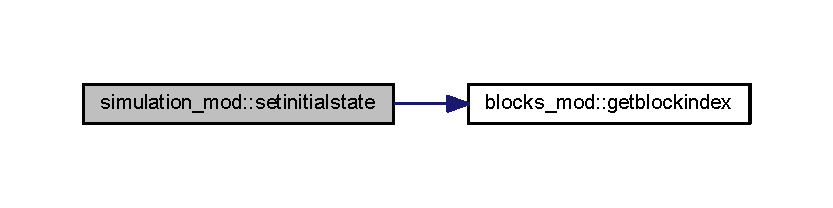
\includegraphics[width=350pt]{namespacesimulation__mod_a447c6d709de6aa360a65d39d660e627b_cgraph}
\end{center}
\end{figure}
\mbox{\Hypertarget{namespacesimulation__mod_acc5fa823c8dd599de8feda8988c224f2}\label{namespacesimulation__mod_acc5fa823c8dd599de8feda8988c224f2}} 
\index{simulation\+\_\+mod@{simulation\+\_\+mod}!settracermemory@{settracermemory}}
\index{settracermemory@{settracermemory}!simulation\+\_\+mod@{simulation\+\_\+mod}}
\subsubsection{\texorpdfstring{settracermemory()}{settracermemory()}}
{\footnotesize\ttfamily subroutine simulation\+\_\+mod\+::settracermemory (\begin{DoxyParamCaption}\item[{class(\mbox{\hyperlink{structsimulation__mod_1_1simulation__class}{simulation\+\_\+class}}), intent(in)}]{self,  }\item[{integer, intent(in), optional}]{ntrc }\end{DoxyParamCaption})\hspace{0.3cm}{\ttfamily [private]}}



Simulation method to account for Tracer memory consumption. 

\begin{DoxyAuthor}{Author}
Ricardo Birjukovs Canelas -\/ M\+A\+R\+E\+T\+EC 
\end{DoxyAuthor}


Definition at line 337 of file simulation.\+f90.


\begin{DoxyCode}
337     \textcolor{keywordtype}{implicit none}
338     \textcolor{keywordtype}{class}(simulation\_class), \textcolor{keywordtype}{intent(in)} :: self
339     \textcolor{keywordtype}{integer}, \textcolor{keywordtype}{optional}, \textcolor{keywordtype}{intent(in)} :: ntrc
340     \textcolor{keywordtype}{integer} :: sizem, i
341     sizem = 0
342     \textcolor{keywordflow}{do} i=1, \textcolor{keyword}{size}(dblock)
343         sizem = sizem + sizeof(dblock(i)%LTracer) \textcolor{comment}{!this accounts for the array structure}
344         sizem = sizem + sizeof(dummytracer)*dblock(i)%LTracer%getSize() \textcolor{comment}{!this accounts for the contents}
345 \textcolor{keywordflow}{    enddo}
346     \textcolor{keyword}{call }simmemory%setracer(sizem)
347     \textcolor{keywordflow}{if}(\textcolor{keyword}{present}(ntrc)) \textcolor{keywordflow}{then}
348         \textcolor{keyword}{call }simmemory%setNtrc(ntrc)
349         \textcolor{keyword}{call }simmemory%setsizeTrc(sizeof(dummytracer))
350 \textcolor{keywordflow}{    end if}
\end{DoxyCode}
\mbox{\Hypertarget{namespacesimulation__mod_a87a5141e4516b9610a6e4f0d2ff2d719}\label{namespacesimulation__mod_a87a5141e4516b9610a6e4f0d2ff2d719}} 
\index{simulation\+\_\+mod@{simulation\+\_\+mod}!togglesources@{togglesources}}
\index{togglesources@{togglesources}!simulation\+\_\+mod@{simulation\+\_\+mod}}
\subsubsection{\texorpdfstring{togglesources()}{togglesources()}}
{\footnotesize\ttfamily subroutine simulation\+\_\+mod\+::togglesources (\begin{DoxyParamCaption}\item[{class(\mbox{\hyperlink{structsimulation__mod_1_1simulation__class}{simulation\+\_\+class}}), intent(in)}]{self }\end{DoxyParamCaption})\hspace{0.3cm}{\ttfamily [private]}}



Simulation method to activate and deactivate Sources based on the GlobalSim\+Time. 

\begin{DoxyAuthor}{Author}
Ricardo Birjukovs Canelas -\/ M\+A\+R\+E\+T\+EC 
\end{DoxyAuthor}


Definition at line 176 of file simulation.\+f90.


\begin{DoxyCode}
176     \textcolor{keywordtype}{implicit none}
177     \textcolor{keywordtype}{class}(simulation\_class), \textcolor{keywordtype}{intent(in)} :: self
178     \textcolor{keywordtype}{integer} :: i
179     \textcolor{keywordflow}{do} i=1, \textcolor{keyword}{size}(dblock)
180         \textcolor{keyword}{call }dblock(i)%ToogleBlockSources()
181 \textcolor{keywordflow}{    enddo}
\end{DoxyCode}

\hypertarget{namespacesimulationabout__mod}{}\section{simulationabout\+\_\+mod Module Reference}
\label{namespacesimulationabout__mod}\index{simulationabout\+\_\+mod@{simulationabout\+\_\+mod}}


Module to print version, licence, preambles.  


\subsection*{Functions/\+Subroutines}
\begin{DoxyCompactItemize}
\item 
subroutine, public \mbox{\hyperlink{namespacesimulationabout__mod_a4248c37e1b337cda7226a41aac346761}{printlicpreamble}}
\begin{DoxyCompactList}\small\item\em Public licence and preamble printer routine. \end{DoxyCompactList}\end{DoxyCompactItemize}
\subsection*{Variables}
\begin{DoxyCompactItemize}
\item 
type(string) \mbox{\hyperlink{namespacesimulationabout__mod_ab3a538e4f741e6ea5be60e667a966fda}{version}}
\item 
type(string) \mbox{\hyperlink{namespacesimulationabout__mod_a64b9a218dda33c3c5abdf4503b71e8a4}{author}}
\item 
type(string) \mbox{\hyperlink{namespacesimulationabout__mod_ab8debffcb94d9718e06501a71218ef26}{date}}
\end{DoxyCompactItemize}


\subsection{Detailed Description}
Module to print version, licence, preambles. 

\begin{DoxyAuthor}{Author}
Ricardo Birjukovs Canelas 
\end{DoxyAuthor}


\subsection{Function/\+Subroutine Documentation}
\mbox{\Hypertarget{namespacesimulationabout__mod_a4248c37e1b337cda7226a41aac346761}\label{namespacesimulationabout__mod_a4248c37e1b337cda7226a41aac346761}} 
\index{simulationabout\+\_\+mod@{simulationabout\+\_\+mod}!printlicpreamble@{printlicpreamble}}
\index{printlicpreamble@{printlicpreamble}!simulationabout\+\_\+mod@{simulationabout\+\_\+mod}}
\subsubsection{\texorpdfstring{printlicpreamble()}{printlicpreamble()}}
{\footnotesize\ttfamily subroutine, public simulationabout\+\_\+mod\+::printlicpreamble (\begin{DoxyParamCaption}{ }\end{DoxyParamCaption})}



Public licence and preamble printer routine. 

\begin{DoxyAuthor}{Author}
Ricardo Birjukovs Canelas -\/ M\+A\+R\+E\+T\+EC 
\end{DoxyAuthor}


Definition at line 44 of file simulation\+About.\+f90.


\begin{DoxyCode}
44     \textcolor{keywordtype}{implicit none}
45     \textcolor{keywordtype}{type}(string) :: outext
46 
47     version  =\textcolor{stringliteral}{"v0.2"}
48     author   =\textcolor{stringliteral}{"R. Birjukovs Canelas - D. Garaboa Paz"}
49     date     =\textcolor{stringliteral}{"25-09-2019"}
50 
51     outext = \textcolor{stringliteral}{' \_\_  \_\_  \_\_\_  \_   \_ \_\_\_ \_\_\_\_  \_                                      \_              '}//
      new\_line(\textcolor{stringliteral}{'a'})//&
52         \textcolor{stringliteral}{' |  \(\backslash\)/  |/ \_ \(\backslash\)| | | |\_ \_|  \_ \(\backslash\)| |    \_\_ \_  \_\_ \_ \_ \_\_ \_\_ \_ \_ \_\_   \_\_ \_(\_) \_\_ \_ \_ \_\_  '}//new\_line(\textcolor{stringliteral}{
      'a'})//&
53         \textcolor{stringliteral}{' | |\(\backslash\)/| | | | | |\_| || || | | | |   / \_` |/ \_` | \_\_/  \_` |  \_ \(\backslash\) / \_` | |/ \_` |  \_ \(\backslash\) '}//new\_line(\textcolor{stringliteral}{
      'a'})//&
54         \textcolor{stringliteral}{' | |  | | |\_| |  \_  || || |\_| | |\_\_| (\_| | (\_| | | | (\_| | | | | (\_| | | (\_| | | | |'}//new\_line(\textcolor{stringliteral}{
      'a'})//&
55         \textcolor{stringliteral}{' |\_|  |\_|\(\backslash\)\_\_\_/|\_| |\_|\_\_\_|\_\_\_\_/|\_\_\_\_\_\(\backslash\)\_\_,\_|\(\backslash\)\_\_, |\_|  \(\backslash\)\_\_,\_|\_| |\_|\(\backslash\)\_\_, |\_|\(\backslash\)\_\_,\_|\_| |\_|'}//new\_line(\textcolor{stringliteral}{
      'a'})//&
56         \textcolor{stringliteral}{'                                          |\_\_\_/                 |\_\_\_/               '}//new\_line(\textcolor{stringliteral}{
      'a'})//&
57 
58         \textcolor{stringliteral}{'  <MOHIDLagrangian> Copyright (C) 2018 by'}//new\_line(\textcolor{stringliteral}{'a'})//&
59         \textcolor{stringliteral}{'  R. Birjukovs Canelas'}//new\_line(\textcolor{stringliteral}{'a'})//&
60         \textcolor{stringliteral}{'  MARETEC - Research Centre for Marine, Environment and Technology'}//new\_line(\textcolor{stringliteral}{'a'})//&
61         \textcolor{stringliteral}{'  University of Lisbon - IST'}//new\_line(\textcolor{stringliteral}{'a'})//&
62         \textcolor{stringliteral}{'  A. Daniel Garaboa Paz'}//new\_line(\textcolor{stringliteral}{'a'})//&
63         \textcolor{stringliteral}{'  Non-Linear Physics Group - University of Santiago de Compostela, Spain'}//new\_line(\textcolor{stringliteral}{'a'})//&
64         \textcolor{stringliteral}{''}//new\_line(\textcolor{stringliteral}{'a'})//&
65         \textcolor{stringliteral}{'  MOHID Lagrangian is free software: you can redistribute it and/or'}//new\_line(\textcolor{stringliteral}{'a'})//&
66         \textcolor{stringliteral}{'  modify it under the terms of the GNU General Public License as'}//new\_line(\textcolor{stringliteral}{'a'})//&
67         \textcolor{stringliteral}{'  published by the Free Software Foundation, either version 3 of'}//new\_line(\textcolor{stringliteral}{'a'})//&
68         \textcolor{stringliteral}{'  the License, or (at your option) any later version.'}//new\_line(\textcolor{stringliteral}{'a'})//&
69         \textcolor{stringliteral}{''}//new\_line(\textcolor{stringliteral}{'a'})//&
70         \textcolor{stringliteral}{'  MOHID Lagrangian is distributed WITHOUT ANY WARRANTY; without even'}//new\_line(\textcolor{stringliteral}{'a'})//&
71         \textcolor{stringliteral}{'  the implied warranty of MERCHANTABILITY or FITNESS FOR A PARTICULAR'}//new\_line(\textcolor{stringliteral}{'a'})//&
72         \textcolor{stringliteral}{'  PURPOSE. See the GNU General Public License for more details.'}//new\_line(\textcolor{stringliteral}{'a'})//&
73         \textcolor{stringliteral}{''}//new\_line(\textcolor{stringliteral}{'a'})//&
74         \textcolor{stringliteral}{'  You should have received a copy of the GNU General Public License,'}//new\_line(\textcolor{stringliteral}{'a'})//&
75         \textcolor{stringliteral}{'  along with MOHID Lagrangian. If not, see <http://www.gnu.org/licenses/>.,'}//new\_line(\textcolor{stringliteral}{'a'})//&
76         \textcolor{stringliteral}{''}//new\_line(\textcolor{stringliteral}{'a'})//&
77         \textcolor{stringliteral}{''}//new\_line(\textcolor{stringliteral}{'a'})//&
78         \textcolor{stringliteral}{'MOHID Lagrangian '}//version//\textcolor{stringliteral}{' ('}//author//\textcolor{stringliteral}{') ('}//date//\textcolor{stringliteral}{')'}//new\_line(\textcolor{stringliteral}{'a'})//&
79         \textcolor{stringliteral}{'====================================================================='}
80 
81     \textcolor{keyword}{call }log%put(outext,.false.)
82 
\end{DoxyCode}
Here is the caller graph for this function\+:\nopagebreak
\begin{figure}[H]
\begin{center}
\leavevmode
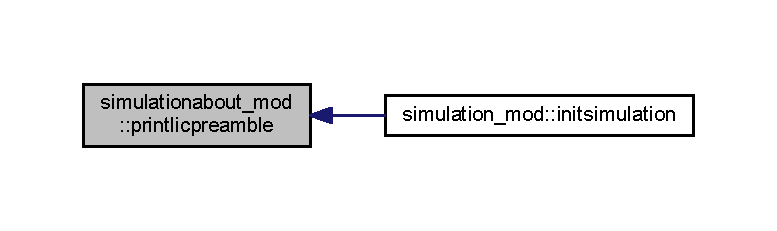
\includegraphics[width=350pt]{namespacesimulationabout__mod_a4248c37e1b337cda7226a41aac346761_icgraph}
\end{center}
\end{figure}


\subsection{Variable Documentation}
\mbox{\Hypertarget{namespacesimulationabout__mod_a64b9a218dda33c3c5abdf4503b71e8a4}\label{namespacesimulationabout__mod_a64b9a218dda33c3c5abdf4503b71e8a4}} 
\index{simulationabout\+\_\+mod@{simulationabout\+\_\+mod}!author@{author}}
\index{author@{author}!simulationabout\+\_\+mod@{simulationabout\+\_\+mod}}
\subsubsection{\texorpdfstring{author}{author}}
{\footnotesize\ttfamily type(string) simulationabout\+\_\+mod\+::author\hspace{0.3cm}{\ttfamily [private]}}



Definition at line 31 of file simulation\+About.\+f90.


\begin{DoxyCode}
31     \textcolor{keywordtype}{type}(string) :: author
\end{DoxyCode}
\mbox{\Hypertarget{namespacesimulationabout__mod_ab8debffcb94d9718e06501a71218ef26}\label{namespacesimulationabout__mod_ab8debffcb94d9718e06501a71218ef26}} 
\index{simulationabout\+\_\+mod@{simulationabout\+\_\+mod}!date@{date}}
\index{date@{date}!simulationabout\+\_\+mod@{simulationabout\+\_\+mod}}
\subsubsection{\texorpdfstring{date}{date}}
{\footnotesize\ttfamily type(string) simulationabout\+\_\+mod\+::date\hspace{0.3cm}{\ttfamily [private]}}



Definition at line 32 of file simulation\+About.\+f90.


\begin{DoxyCode}
32     \textcolor{keywordtype}{type}(string) :: date
\end{DoxyCode}
\mbox{\Hypertarget{namespacesimulationabout__mod_ab3a538e4f741e6ea5be60e667a966fda}\label{namespacesimulationabout__mod_ab3a538e4f741e6ea5be60e667a966fda}} 
\index{simulationabout\+\_\+mod@{simulationabout\+\_\+mod}!version@{version}}
\index{version@{version}!simulationabout\+\_\+mod@{simulationabout\+\_\+mod}}
\subsubsection{\texorpdfstring{version}{version}}
{\footnotesize\ttfamily type(string) simulationabout\+\_\+mod\+::version\hspace{0.3cm}{\ttfamily [private]}}



Definition at line 30 of file simulation\+About.\+f90.


\begin{DoxyCode}
30     \textcolor{keywordtype}{type}(string) :: version
\end{DoxyCode}

\hypertarget{namespacesimulationglobals__mod}{}\section{simulationglobals\+\_\+mod Module Reference}
\label{namespacesimulationglobals__mod}\index{simulationglobals\+\_\+mod@{simulationglobals\+\_\+mod}}


Module to hold the simulation global parameter classes and their methods.  


\subsection*{Data Types}
\begin{DoxyCompactItemize}
\item 
type \mbox{\hyperlink{structsimulationglobals__mod_1_1constants__t}{constants\+\_\+t}}
\begin{DoxyCompactList}\small\item\em Case Constants class. \end{DoxyCompactList}\item 
type \mbox{\hyperlink{structsimulationglobals__mod_1_1datatypes__t}{datatypes\+\_\+t}}
\item 
type \mbox{\hyperlink{structsimulationglobals__mod_1_1filenames__t}{filenames\+\_\+t}}
\begin{DoxyCompactList}\small\item\em File names class. \end{DoxyCompactList}\item 
type \mbox{\hyperlink{structsimulationglobals__mod_1_1globals__class}{globals\+\_\+class}}
\begin{DoxyCompactList}\small\item\em Globals class -\/ This is a container for every global variable on the simulation. \end{DoxyCompactList}\item 
type \mbox{\hyperlink{structsimulationglobals__mod_1_1maskvals__t}{maskvals\+\_\+t}}
\item 
type \mbox{\hyperlink{structsimulationglobals__mod_1_1output__t}{output\+\_\+t}}
\begin{DoxyCompactList}\small\item\em Simulation related counters and others. \end{DoxyCompactList}\item 
type \mbox{\hyperlink{structsimulationglobals__mod_1_1parameters__t}{parameters\+\_\+t}}
\item 
type \mbox{\hyperlink{structsimulationglobals__mod_1_1sim__t}{sim\+\_\+t}}
\begin{DoxyCompactList}\small\item\em Simulation related counters and others. \end{DoxyCompactList}\item 
type \mbox{\hyperlink{structsimulationglobals__mod_1_1sim__time__t}{sim\+\_\+time\+\_\+t}}
\item 
type \mbox{\hyperlink{structsimulationglobals__mod_1_1simdefs__t}{simdefs\+\_\+t}}
\begin{DoxyCompactList}\small\item\em Simulation definitions class. \end{DoxyCompactList}\item 
type \mbox{\hyperlink{structsimulationglobals__mod_1_1sources__t}{sources\+\_\+t}}
\item 
type \mbox{\hyperlink{structsimulationglobals__mod_1_1stringlist__class}{stringlist\+\_\+class}}
\item 
type \mbox{\hyperlink{structsimulationglobals__mod_1_1tracertypes__t}{tracertypes\+\_\+t}}
\item 
type \mbox{\hyperlink{structsimulationglobals__mod_1_1var__names__t}{var\+\_\+names\+\_\+t}}
\end{DoxyCompactItemize}
\subsection*{Functions/\+Subroutines}
\begin{DoxyCompactItemize}
\item 
subroutine \mbox{\hyperlink{namespacesimulationglobals__mod_aa01e0a958ef2e94a02991dcfe390bfa0}{setdefaults}} (self, outpath)
\begin{DoxyCompactList}\small\item\em Globals default setting routine. \end{DoxyCompactList}\item 
subroutine \mbox{\hyperlink{namespacesimulationglobals__mod_a4aa829af1699c705e46f47bb023ac162}{buildvars}} (self)
\begin{DoxyCompactList}\small\item\em Builds variable list names. \end{DoxyCompactList}\item 
subroutine \mbox{\hyperlink{namespacesimulationglobals__mod_afd372c5764a180f9029d4dc3cddce94d}{addvar}} (self, var)
\begin{DoxyCompactList}\small\item\em adding variables to variable pool of a simulation \end{DoxyCompactList}\item 
type(string) function \mbox{\hyperlink{namespacesimulationglobals__mod_ac83c53dd4e998e653981c7b1fa5dacbd}{getvarsimname}} (self, var)
\begin{DoxyCompactList}\small\item\em returns the simulation name of a given variabe name, by brute force searching trough the naming variable lists... \end{DoxyCompactList}\item 
subroutine \mbox{\hyperlink{namespacesimulationglobals__mod_a422e3d203aad010489f541f645f63517}{setinputfilenames}} (self, filenames)
\begin{DoxyCompactList}\small\item\em set the name of the input data files \end{DoxyCompactList}\item 
subroutine \mbox{\hyperlink{namespacesimulationglobals__mod_affd52c4c7b1c3f7ce282eeb7e4b4a359}{setnamingconventions}} (self, filename)
\begin{DoxyCompactList}\small\item\em set the naming conventions. Imports names from given .xml naming files \end{DoxyCompactList}\item 
subroutine \mbox{\hyperlink{namespacesimulationglobals__mod_a2c6fa0a9123d06b2110258ea200f4f52}{setvarnames}} (self, var\+Node)
\begin{DoxyCompactList}\small\item\em set the variables naming conventions. \end{DoxyCompactList}\item 
subroutine \mbox{\hyperlink{namespacesimulationglobals__mod_a878fdcfa67037a1bc8411995394c2bef}{setdimnames}} (self, dim\+Node)
\begin{DoxyCompactList}\small\item\em set the dimensions naming conventions. \end{DoxyCompactList}\item 
subroutine \mbox{\hyperlink{namespacesimulationglobals__mod_a4dd64cb7a896b62d90e20a7eab65a6bf}{setcurrvar}} (self, tag, curr\+Var, curr\+Var\+Name\+List, var\+Node)
\begin{DoxyCompactList}\small\item\em set the current variable naming conventions. Imports the variable names from given .xml naming file. If the same variable is given again two things happen\+: a) the system name is overwriten; b) new variants are added to the name variant list \end{DoxyCompactList}\item 
subroutine \mbox{\hyperlink{namespacesimulationglobals__mod_aefda4344f03a705055ad6cb97cb90c65}{settimedate}} (self)
\begin{DoxyCompactList}\small\item\em initializes time stamp and date stamp variables \end{DoxyCompactList}\item 
subroutine \mbox{\hyperlink{namespacesimulationglobals__mod_acbb28eee5547a03dc28c924d8e23ad9a}{setcurrdatetime}} (self, dt)
\begin{DoxyCompactList}\small\item\em sets the current time stamp and date stamp given a dt increment \end{DoxyCompactList}\item 
real(prec) function \mbox{\hyperlink{namespacesimulationglobals__mod_a1fd33b50ae2216b3b7db074da1672398}{getdatetimestamp}} (self)
\begin{DoxyCompactList}\small\item\em returns the time stamp for the current time/date. Time Stamp is days since epoch, given by Base\+Date\+Time. Defaults to Copernicus standard. \end{DoxyCompactList}\item 
subroutine \mbox{\hyperlink{namespacesimulationglobals__mod_abd0e28a5ec7733d0292dd8e631e96577}{printdatetime}} (self)
\begin{DoxyCompactList}\small\item\em prints date \& time information. \end{DoxyCompactList}\item 
subroutine \mbox{\hyperlink{namespacesimulationglobals__mod_a3f11ed9f7735018950e1921ead871269}{increment\+\_\+numtracer}} (self)
\begin{DoxyCompactList}\small\item\em Increments Tracer count. This routine M\+U\+ST be A\+T\+O\+M\+IC. \end{DoxyCompactList}\item 
integer function \mbox{\hyperlink{namespacesimulationglobals__mod_ac4915156236196940b31ff02d53af295}{getnumtracer}} (self)
\begin{DoxyCompactList}\small\item\em Returns a new ID for a Tracer. \end{DoxyCompactList}\item 
subroutine \mbox{\hyperlink{namespacesimulationglobals__mod_ad983ee8885b275c6fa1369f1e158e078}{increment\+\_\+numdt}} (self)
\begin{DoxyCompactList}\small\item\em incrementing time step count. \end{DoxyCompactList}\item 
integer function \mbox{\hyperlink{namespacesimulationglobals__mod_af313959d6cbfc4cb0ab330aa094511c5}{getnumdt}} (self)
\begin{DoxyCompactList}\small\item\em Returns the number of time steps. \end{DoxyCompactList}\item 
integer function \mbox{\hyperlink{namespacesimulationglobals__mod_ac643661b27d17726e0305e34370de5c3}{getlastoutnumdt}} (self)
\begin{DoxyCompactList}\small\item\em Returns the number of time steps from last ouptut. \end{DoxyCompactList}\item 
subroutine \mbox{\hyperlink{namespacesimulationglobals__mod_ab760ab6064743ff54237166301346616}{setlastoutnumdt}} (self, num)
\begin{DoxyCompactList}\small\item\em Sets the number of time steps from last ouptut. \end{DoxyCompactList}\item 
subroutine \mbox{\hyperlink{namespacesimulationglobals__mod_a77d7175bc03e472ee9a00ee9f6ff1b0e}{increment\+\_\+numoutfile}} (self)
\begin{DoxyCompactList}\small\item\em incrementing output file count. \end{DoxyCompactList}\item 
integer function \mbox{\hyperlink{namespacesimulationglobals__mod_a2b76dc3e6cbf1256253c54903df8393b}{getnumoutfile}} (self)
\begin{DoxyCompactList}\small\item\em Returns the number of output files written. \end{DoxyCompactList}\item 
subroutine \mbox{\hyperlink{namespacesimulationglobals__mod_a1b94fa3858d556fc974a7ac6b18625cb}{addtooutputpool}} (self, var)
\begin{DoxyCompactList}\small\item\em adds a variable name to the output pool. \end{DoxyCompactList}\item 
subroutine \mbox{\hyperlink{namespacesimulationglobals__mod_a046b75c2e163809ea467da6340f1829c}{setoutputfields}} (self, fields, to\+Output)
\begin{DoxyCompactList}\small\item\em adds variable fields one by one to the output pool, given a string and boolean list. \end{DoxyCompactList}\item 
subroutine \mbox{\hyperlink{namespacesimulationglobals__mod_ac0323793c29be7c79a735ca766fb8a78}{getoutputpoolarray}} (self, array)
\begin{DoxyCompactList}\small\item\em adds a variable name to the output pool. \end{DoxyCompactList}\item 
logical function \mbox{\hyperlink{namespacesimulationglobals__mod_a17dc711ec02d5aea0c33006939da8dec}{inoutputpool}} (self, var)
\begin{DoxyCompactList}\small\item\em Returns true if a given var is in the output pool. \end{DoxyCompactList}\item 
subroutine \mbox{\hyperlink{namespacesimulationglobals__mod_ada0b6ffc5e112afbd86cdaa8d9aa55d8}{setparam}} (self, parmkey, parmvalue)
\begin{DoxyCompactList}\small\item\em Private parameter setting method. Builds the simulation parametric space from the input case file. \end{DoxyCompactList}\item 
subroutine \mbox{\hyperlink{namespacesimulationglobals__mod_a3d337e9c28136dd9c67fa576f05cd44b}{check}} (self)
\begin{DoxyCompactList}\small\item\em Parameter checking method. Checks if mandatory parameters were set. \end{DoxyCompactList}\item 
subroutine \mbox{\hyperlink{namespacesimulationglobals__mod_ab67964fe7c3fb20a4ce0b4193520aa1d}{printsimparameters}} (self)
\begin{DoxyCompactList}\small\item\em Parameter printing method. \end{DoxyCompactList}\item 
subroutine \mbox{\hyperlink{namespacesimulationglobals__mod_ae6b88d15ddc389aedd73d600de0337df}{setgravity}} (self, grav)
\begin{DoxyCompactList}\small\item\em Gravity setting routine. \end{DoxyCompactList}\item 
subroutine \mbox{\hyperlink{namespacesimulationglobals__mod_a36c2833caae3767434115cc966fe2c5d}{setz0}} (self, read\+\_\+z0)
\begin{DoxyCompactList}\small\item\em Z0 setting routine. \end{DoxyCompactList}\item 
subroutine \mbox{\hyperlink{namespacesimulationglobals__mod_a7d41fc05216d326ae8c0b090362430d3}{setrho}} (self, read\+\_\+rho)
\begin{DoxyCompactList}\small\item\em Rho\+Ref setting routine. \end{DoxyCompactList}\item 
subroutine \mbox{\hyperlink{namespacesimulationglobals__mod_a3b24d0338ee34782c8e2ab57bba7b5f6}{setbeachinglevel}} (self, read\+\_\+\+Beaching\+Level)
\begin{DoxyCompactList}\small\item\em Beaching Level setting routine. \end{DoxyCompactList}\item 
subroutine \mbox{\hyperlink{namespacesimulationglobals__mod_aacd46eb198a99699d7be61b807363fc6}{setbeachingstopprob}} (self, read\+\_\+\+Beaching\+Stop\+Prob)
\begin{DoxyCompactList}\small\item\em Beaching stop probability setting routine. \end{DoxyCompactList}\item 
subroutine \mbox{\hyperlink{namespacesimulationglobals__mod_a70465a87d621a450f8b100fad0d29bc9}{setdiffusioncoeff}} (self, read\+\_\+\+Diffusion\+Coeff)
\begin{DoxyCompactList}\small\item\em Horizontal Diffusion coefficient setting routine. \end{DoxyCompactList}\item 
subroutine \mbox{\hyperlink{namespacesimulationglobals__mod_ad36c21a592a3230ce848804075abc97e}{setsmalldt}} (self, dt)
\begin{DoxyCompactList}\small\item\em small\+Dt setting routine. \end{DoxyCompactList}\item 
subroutine \mbox{\hyperlink{namespacesimulationglobals__mod_a139cb36f8366e6aec875c7977235fd68}{printconstants}} (self)
\begin{DoxyCompactList}\small\item\em Public constants printing routine. \end{DoxyCompactList}\item 
subroutine \mbox{\hyperlink{namespacesimulationglobals__mod_afda1e73e6e0cd075875c70aded99d425}{setdp}} (self, read\+\_\+dp)
\begin{DoxyCompactList}\small\item\em Dp setting routine. \end{DoxyCompactList}\item 
subroutine \mbox{\hyperlink{namespacesimulationglobals__mod_a0eced3f4367d08f3d0cb6ef2044bdc56}{setdt}} (self, read\+\_\+dt)
\begin{DoxyCompactList}\small\item\em Dt setting routine. \end{DoxyCompactList}\item 
subroutine \mbox{\hyperlink{namespacesimulationglobals__mod_abf5afcc12763caab3a5fc394255ced44}{setboundingbox}} (self, point\+\_\+, coords)
\begin{DoxyCompactList}\small\item\em Bounding box setting routine. \end{DoxyCompactList}\item 
subroutine \mbox{\hyperlink{namespacesimulationglobals__mod_af0bc0b00ee3aa2ba9e47dc50daa72799}{setblocksize}} (self, bsize)
\begin{DoxyCompactList}\small\item\em blocksize box setting routine \end{DoxyCompactList}\item 
subroutine \mbox{\hyperlink{namespacesimulationglobals__mod_a54196bff569fc838730ba39a722319ff}{printsimdefs}} (self)
\begin{DoxyCompactList}\small\item\em Public simulation definitions printing routine. \end{DoxyCompactList}\item 
subroutine \mbox{\hyperlink{namespacesimulationglobals__mod_a7adb33aaa9ea0a94c38789c07ff3e787}{print\+\_\+stringlist}} (this)
\begin{DoxyCompactList}\small\item\em Method that prints all the links of the list. \end{DoxyCompactList}\item 
subroutine \mbox{\hyperlink{namespacesimulationglobals__mod_a405f70548e38f0af65d4cbdb7c7025a4}{print\+\_\+stringlistcurrent}} (this)
\begin{DoxyCompactList}\small\item\em Method that prints the current link of the list. \end{DoxyCompactList}\item 
logical function \mbox{\hyperlink{namespacesimulationglobals__mod_a12410ee549ead4c6d892dca6ead74d15}{notrepeated}} (this, str)
\begin{DoxyCompactList}\small\item\em Method that checks if an element is already on the list. Returns false if it is. \end{DoxyCompactList}\end{DoxyCompactItemize}
\subsection*{Variables}
\begin{DoxyCompactItemize}
\item 
type(string), public \mbox{\hyperlink{namespacesimulationglobals__mod_a359d52eab96ddcaba05e0504eff0ef37}{notread}}
\item 
type(string), public \mbox{\hyperlink{namespacesimulationglobals__mod_a34d00a17e5931ddf3ab1a361f6299ae3}{notset}}
\item 
type(\mbox{\hyperlink{structsimulationglobals__mod_1_1globals__class}{globals\+\_\+class}}), public \mbox{\hyperlink{namespacesimulationglobals__mod_acf1e2786d81bd0fe337a8458efce8733}{globals}}
\end{DoxyCompactItemize}


\subsection{Detailed Description}
Module to hold the simulation global parameter classes and their methods. 

\begin{DoxyAuthor}{Author}
Ricardo Birjukovs Canelas 
\end{DoxyAuthor}


\subsection{Function/\+Subroutine Documentation}
\mbox{\Hypertarget{namespacesimulationglobals__mod_a1b94fa3858d556fc974a7ac6b18625cb}\label{namespacesimulationglobals__mod_a1b94fa3858d556fc974a7ac6b18625cb}} 
\index{simulationglobals\+\_\+mod@{simulationglobals\+\_\+mod}!addtooutputpool@{addtooutputpool}}
\index{addtooutputpool@{addtooutputpool}!simulationglobals\+\_\+mod@{simulationglobals\+\_\+mod}}
\subsubsection{\texorpdfstring{addtooutputpool()}{addtooutputpool()}}
{\footnotesize\ttfamily subroutine simulationglobals\+\_\+mod\+::addtooutputpool (\begin{DoxyParamCaption}\item[{class(\mbox{\hyperlink{structsimulationglobals__mod_1_1output__t}{output\+\_\+t}}), intent(inout)}]{self,  }\item[{type(string), intent(in)}]{var }\end{DoxyParamCaption})\hspace{0.3cm}{\ttfamily [private]}}



adds a variable name to the output pool. 

\begin{DoxyAuthor}{Author}
Ricardo Birjukovs Canelas -\/ M\+A\+R\+E\+T\+EC 
\end{DoxyAuthor}


Definition at line 765 of file simulation\+Globals.\+f90.


\begin{DoxyCode}
765     \textcolor{keywordtype}{class}(output\_t), \textcolor{keywordtype}{intent(inout)} :: self
766     \textcolor{keywordtype}{type}(string), \textcolor{keywordtype}{intent(in)} :: var
767     \textcolor{keywordflow}{if} (self%varToOutput%notRepeated(var)) \textcolor{keyword}{call }self%varToOutput%add(var)
\end{DoxyCode}
\mbox{\Hypertarget{namespacesimulationglobals__mod_afd372c5764a180f9029d4dc3cddce94d}\label{namespacesimulationglobals__mod_afd372c5764a180f9029d4dc3cddce94d}} 
\index{simulationglobals\+\_\+mod@{simulationglobals\+\_\+mod}!addvar@{addvar}}
\index{addvar@{addvar}!simulationglobals\+\_\+mod@{simulationglobals\+\_\+mod}}
\subsubsection{\texorpdfstring{addvar()}{addvar()}}
{\footnotesize\ttfamily subroutine simulationglobals\+\_\+mod\+::addvar (\begin{DoxyParamCaption}\item[{class(\mbox{\hyperlink{structsimulationglobals__mod_1_1var__names__t}{var\+\_\+names\+\_\+t}}), intent(inout)}]{self,  }\item[{type(string), intent(in)}]{var }\end{DoxyParamCaption})\hspace{0.3cm}{\ttfamily [private]}}



adding variables to variable pool of a simulation 

\begin{DoxyAuthor}{Author}
Ricardo Birjukovs Canelas -\/ M\+A\+R\+E\+T\+EC 
\end{DoxyAuthor}


Definition at line 384 of file simulation\+Globals.\+f90.


\begin{DoxyCode}
384     \textcolor{keywordtype}{class}(var\_names\_t), \textcolor{keywordtype}{intent(inout)} :: self
385     \textcolor{keywordtype}{type}(string), \textcolor{keywordtype}{intent(in)} :: var
386     \textcolor{keywordflow}{if} (self%varToUse%notRepeated(var)) \textcolor{keyword}{call }self%varToUse%add(var)
\end{DoxyCode}
\mbox{\Hypertarget{namespacesimulationglobals__mod_a4aa829af1699c705e46f47bb023ac162}\label{namespacesimulationglobals__mod_a4aa829af1699c705e46f47bb023ac162}} 
\index{simulationglobals\+\_\+mod@{simulationglobals\+\_\+mod}!buildvars@{buildvars}}
\index{buildvars@{buildvars}!simulationglobals\+\_\+mod@{simulationglobals\+\_\+mod}}
\subsubsection{\texorpdfstring{buildvars()}{buildvars()}}
{\footnotesize\ttfamily subroutine simulationglobals\+\_\+mod\+::buildvars (\begin{DoxyParamCaption}\item[{class(\mbox{\hyperlink{structsimulationglobals__mod_1_1var__names__t}{var\+\_\+names\+\_\+t}}), intent(inout)}]{self }\end{DoxyParamCaption})\hspace{0.3cm}{\ttfamily [private]}}



Builds variable list names. 

\begin{DoxyAuthor}{Author}
Ricardo Birjukovs Canelas -\/ M\+A\+R\+E\+T\+EC 
\end{DoxyAuthor}


Definition at line 347 of file simulation\+Globals.\+f90.


\begin{DoxyCode}
347     \textcolor{keywordtype}{class}(var\_names\_t), \textcolor{keywordtype}{intent(inout)} :: self
348     self%u       = \textcolor{stringliteral}{'u'}
349     self%v       = \textcolor{stringliteral}{'v'}
350     self%w       = \textcolor{stringliteral}{'w'}
351     self%temp    = \textcolor{stringliteral}{'temp'}
352     self%sal     = \textcolor{stringliteral}{'sal'}
353     self%density = \textcolor{stringliteral}{'density'}
354     self%vsdx    = \textcolor{stringliteral}{'vsdx'}
355     self%vsdy    = \textcolor{stringliteral}{'vsdy'}
356     self%u10     = \textcolor{stringliteral}{'u10'}
357     self%v10     = \textcolor{stringliteral}{'v10'}
358     self%lon     = \textcolor{stringliteral}{'lon'}
359     self%lat     = \textcolor{stringliteral}{'lat'}
360     self%level   = \textcolor{stringliteral}{'level'}
361     self%time    = \textcolor{stringliteral}{'time'}
362     self%landIntMask = \textcolor{stringliteral}{'landIntMask'}
363     self%resolution = \textcolor{stringliteral}{'resolution'}
364     self%rate = \textcolor{stringliteral}{'rate'}
365     \textcolor{comment}{!adding variables to variable pool - PLACEHOLDER, this should come from tracer constructors}
366     \textcolor{keyword}{call }self%addVar(self%u)
367     \textcolor{keyword}{call }self%addVar(self%v)
368     \textcolor{keyword}{call }self%addVar(self%w)
369     \textcolor{keyword}{call }self%addVar(self%temp)
370     \textcolor{keyword}{call }self%addVar(self%sal)
371     \textcolor{keyword}{call }self%addVar(self%density)
372     \textcolor{comment}{!call self%addVar(self%lon)}
373     \textcolor{comment}{!call self%addVar(self%lat)}
374     \textcolor{comment}{!call self%addVar(self%level)}
375     \textcolor{comment}{!call self%addVar(self%time)}
\end{DoxyCode}
\mbox{\Hypertarget{namespacesimulationglobals__mod_a3d337e9c28136dd9c67fa576f05cd44b}\label{namespacesimulationglobals__mod_a3d337e9c28136dd9c67fa576f05cd44b}} 
\index{simulationglobals\+\_\+mod@{simulationglobals\+\_\+mod}!check@{check}}
\index{check@{check}!simulationglobals\+\_\+mod@{simulationglobals\+\_\+mod}}
\subsubsection{\texorpdfstring{check()}{check()}}
{\footnotesize\ttfamily subroutine simulationglobals\+\_\+mod\+::check (\begin{DoxyParamCaption}\item[{class(\mbox{\hyperlink{structsimulationglobals__mod_1_1parameters__t}{parameters\+\_\+t}}), intent(inout)}]{self }\end{DoxyParamCaption})\hspace{0.3cm}{\ttfamily [private]}}



Parameter checking method. Checks if mandatory parameters were set. 

\begin{DoxyAuthor}{Author}
Ricardo Birjukovs Canelas -\/ M\+A\+R\+E\+T\+EC 
\end{DoxyAuthor}


Definition at line 892 of file simulation\+Globals.\+f90.


\begin{DoxyCode}
892     \textcolor{keywordtype}{class}(parameters\_t), \textcolor{keywordtype}{intent(inout)} :: self
893     \textcolor{keywordtype}{type}(string) :: outext
894     \textcolor{keywordtype}{type}(datetime) :: temp
895     \textcolor{keywordtype}{type}(timedelta) :: simtime
896 
897     \textcolor{keywordflow}{if} ( any(self%IntegratorIndexes == self%Integrator)) \textcolor{keywordflow}{then}
898     \textcolor{keywordflow}{else}
899         outext = \textcolor{stringliteral}{'[Globals::parameters::check]: Integrator not recognized, stoping'}
900         \textcolor{keyword}{call }log%put(outext)
901         stop
902 \textcolor{keywordflow}{    end if}
903     \textcolor{keywordflow}{if} ( any(self%OutputFormatIndexes == self%OutputFormat)) \textcolor{keywordflow}{then}
904         \textcolor{keywordflow}{if} (self%OutputFormat == 1) \textcolor{keywordflow}{then}
905             outext = \textcolor{stringliteral}{'[Globals::parameters::check]: NetCDF is not implemented yet, try something nicer like
       VTK, stoping'}
906             \textcolor{keyword}{call }log%put(outext)
907             stop
908 \textcolor{keywordflow}{        end if}
909     \textcolor{keywordflow}{else}
910         outext = \textcolor{stringliteral}{'[Globals::parameters::check]: OutputFormat not recognized, stoping'}
911         \textcolor{keyword}{call }log%put(outext)
912         stop
913 \textcolor{keywordflow}{    end if}
914     temp = datetime() \textcolor{comment}{!default initialization}
915     \textcolor{comment}{!add new parameters to this search}
916     \textcolor{keywordflow}{if} (self%OutputWriteTime==mv) \textcolor{keywordflow}{then}
917         outext = \textcolor{stringliteral}{'[Globals::parameters::check]: Output sampling rate parameter (OutputWriteTime) is not
       set, stoping'}
918         \textcolor{keyword}{call }log%put(outext)
919         stop
920     \textcolor{keywordflow}{elseif} (self%StartTime==temp) \textcolor{keywordflow}{then}
921         outext = \textcolor{stringliteral}{'[Globals::parameters::check]: start time parameter (Start) is not set or invalid,
       stoping'}
922         \textcolor{keyword}{call }log%put(outext)
923         stop
924     \textcolor{keywordflow}{elseif} (self%EndTime==temp) \textcolor{keywordflow}{then}
925         outext = \textcolor{stringliteral}{'[Globals::parameters::check]: end time parameter (End) is not set or invalid, stoping'}
926         \textcolor{keyword}{call }log%put(outext)
927         stop
928 \textcolor{keywordflow}{    end if}
929     \textcolor{comment}{!Build timemax from the difference between start and end time}
930     simtime = self%EndTime - self%StartTime
931     self%TimeMax = simtime%total\_seconds()
\end{DoxyCode}
\mbox{\Hypertarget{namespacesimulationglobals__mod_a1fd33b50ae2216b3b7db074da1672398}\label{namespacesimulationglobals__mod_a1fd33b50ae2216b3b7db074da1672398}} 
\index{simulationglobals\+\_\+mod@{simulationglobals\+\_\+mod}!getdatetimestamp@{getdatetimestamp}}
\index{getdatetimestamp@{getdatetimestamp}!simulationglobals\+\_\+mod@{simulationglobals\+\_\+mod}}
\subsubsection{\texorpdfstring{getdatetimestamp()}{getdatetimestamp()}}
{\footnotesize\ttfamily real(prec) function simulationglobals\+\_\+mod\+::getdatetimestamp (\begin{DoxyParamCaption}\item[{class(\mbox{\hyperlink{structsimulationglobals__mod_1_1sim__time__t}{sim\+\_\+time\+\_\+t}}), intent(inout)}]{self }\end{DoxyParamCaption})\hspace{0.3cm}{\ttfamily [private]}}



returns the time stamp for the current time/date. Time Stamp is days since epoch, given by Base\+Date\+Time. Defaults to Copernicus standard. 

\begin{DoxyAuthor}{Author}
Ricardo Birjukovs Canelas -\/ M\+A\+R\+E\+T\+EC 
\end{DoxyAuthor}


Definition at line 645 of file simulation\+Globals.\+f90.


\begin{DoxyCode}
645     \textcolor{keywordtype}{class}(sim\_time\_t), \textcolor{keywordtype}{intent(inout)} :: self
646     \textcolor{keywordtype}{type}(timedelta) :: step, day
647     day = timedelta(days=1)
648     step = self%CurrDate - self%BaseDateTime
649     getdatetimestamp = step%total\_seconds()/day%total\_seconds()
\end{DoxyCode}
\mbox{\Hypertarget{namespacesimulationglobals__mod_ac643661b27d17726e0305e34370de5c3}\label{namespacesimulationglobals__mod_ac643661b27d17726e0305e34370de5c3}} 
\index{simulationglobals\+\_\+mod@{simulationglobals\+\_\+mod}!getlastoutnumdt@{getlastoutnumdt}}
\index{getlastoutnumdt@{getlastoutnumdt}!simulationglobals\+\_\+mod@{simulationglobals\+\_\+mod}}
\subsubsection{\texorpdfstring{getlastoutnumdt()}{getlastoutnumdt()}}
{\footnotesize\ttfamily integer function simulationglobals\+\_\+mod\+::getlastoutnumdt (\begin{DoxyParamCaption}\item[{class(\mbox{\hyperlink{structsimulationglobals__mod_1_1output__t}{output\+\_\+t}}), intent(inout)}]{self }\end{DoxyParamCaption})\hspace{0.3cm}{\ttfamily [private]}}



Returns the number of time steps from last ouptut. 

\begin{DoxyAuthor}{Author}
Ricardo Birjukovs Canelas -\/ M\+A\+R\+E\+T\+EC 
\end{DoxyAuthor}


Definition at line 724 of file simulation\+Globals.\+f90.


\begin{DoxyCode}
724     \textcolor{keywordtype}{class}(output\_t), \textcolor{keywordtype}{intent(inout)} :: self
725     getlastoutnumdt = self%lastOutNumDt
\end{DoxyCode}
\mbox{\Hypertarget{namespacesimulationglobals__mod_af313959d6cbfc4cb0ab330aa094511c5}\label{namespacesimulationglobals__mod_af313959d6cbfc4cb0ab330aa094511c5}} 
\index{simulationglobals\+\_\+mod@{simulationglobals\+\_\+mod}!getnumdt@{getnumdt}}
\index{getnumdt@{getnumdt}!simulationglobals\+\_\+mod@{simulationglobals\+\_\+mod}}
\subsubsection{\texorpdfstring{getnumdt()}{getnumdt()}}
{\footnotesize\ttfamily integer function simulationglobals\+\_\+mod\+::getnumdt (\begin{DoxyParamCaption}\item[{class(\mbox{\hyperlink{structsimulationglobals__mod_1_1sim__t}{sim\+\_\+t}}), intent(inout)}]{self }\end{DoxyParamCaption})\hspace{0.3cm}{\ttfamily [private]}}



Returns the number of time steps. 

\begin{DoxyAuthor}{Author}
Ricardo Birjukovs Canelas -\/ M\+A\+R\+E\+T\+EC 
\end{DoxyAuthor}


Definition at line 714 of file simulation\+Globals.\+f90.


\begin{DoxyCode}
714     \textcolor{keywordtype}{class}(sim\_t), \textcolor{keywordtype}{intent(inout)} :: self
715     getnumdt = self%numdt
\end{DoxyCode}
\mbox{\Hypertarget{namespacesimulationglobals__mod_a2b76dc3e6cbf1256253c54903df8393b}\label{namespacesimulationglobals__mod_a2b76dc3e6cbf1256253c54903df8393b}} 
\index{simulationglobals\+\_\+mod@{simulationglobals\+\_\+mod}!getnumoutfile@{getnumoutfile}}
\index{getnumoutfile@{getnumoutfile}!simulationglobals\+\_\+mod@{simulationglobals\+\_\+mod}}
\subsubsection{\texorpdfstring{getnumoutfile()}{getnumoutfile()}}
{\footnotesize\ttfamily integer function simulationglobals\+\_\+mod\+::getnumoutfile (\begin{DoxyParamCaption}\item[{class(\mbox{\hyperlink{structsimulationglobals__mod_1_1output__t}{output\+\_\+t}}), intent(inout)}]{self }\end{DoxyParamCaption})\hspace{0.3cm}{\ttfamily [private]}}



Returns the number of output files written. 

\begin{DoxyAuthor}{Author}
Ricardo Birjukovs Canelas -\/ M\+A\+R\+E\+T\+EC 
\end{DoxyAuthor}


Definition at line 755 of file simulation\+Globals.\+f90.


\begin{DoxyCode}
755     \textcolor{keywordtype}{class}(output\_t), \textcolor{keywordtype}{intent(inout)} :: self
756     getnumoutfile = self%numOutFile
\end{DoxyCode}
\mbox{\Hypertarget{namespacesimulationglobals__mod_ac4915156236196940b31ff02d53af295}\label{namespacesimulationglobals__mod_ac4915156236196940b31ff02d53af295}} 
\index{simulationglobals\+\_\+mod@{simulationglobals\+\_\+mod}!getnumtracer@{getnumtracer}}
\index{getnumtracer@{getnumtracer}!simulationglobals\+\_\+mod@{simulationglobals\+\_\+mod}}
\subsubsection{\texorpdfstring{getnumtracer()}{getnumtracer()}}
{\footnotesize\ttfamily integer function simulationglobals\+\_\+mod\+::getnumtracer (\begin{DoxyParamCaption}\item[{class(\mbox{\hyperlink{structsimulationglobals__mod_1_1sim__t}{sim\+\_\+t}}), intent(inout)}]{self }\end{DoxyParamCaption})\hspace{0.3cm}{\ttfamily [private]}}



Returns a new ID for a Tracer. 

\begin{DoxyAuthor}{Author}
Ricardo Birjukovs Canelas -\/ M\+A\+R\+E\+T\+EC 
\end{DoxyAuthor}


Definition at line 693 of file simulation\+Globals.\+f90.


\begin{DoxyCode}
693     \textcolor{keywordtype}{class}(sim\_t), \textcolor{keywordtype}{intent(inout)} :: self
694     \textcolor{keyword}{call }self%increment\_numTracer()
695     getnumtracer = self%numTracer
\end{DoxyCode}
\mbox{\Hypertarget{namespacesimulationglobals__mod_ac0323793c29be7c79a735ca766fb8a78}\label{namespacesimulationglobals__mod_ac0323793c29be7c79a735ca766fb8a78}} 
\index{simulationglobals\+\_\+mod@{simulationglobals\+\_\+mod}!getoutputpoolarray@{getoutputpoolarray}}
\index{getoutputpoolarray@{getoutputpoolarray}!simulationglobals\+\_\+mod@{simulationglobals\+\_\+mod}}
\subsubsection{\texorpdfstring{getoutputpoolarray()}{getoutputpoolarray()}}
{\footnotesize\ttfamily subroutine simulationglobals\+\_\+mod\+::getoutputpoolarray (\begin{DoxyParamCaption}\item[{class(\mbox{\hyperlink{structsimulationglobals__mod_1_1output__t}{output\+\_\+t}}), intent(inout)}]{self,  }\item[{type(string), dimension(\+:), intent(out), allocatable}]{array }\end{DoxyParamCaption})\hspace{0.3cm}{\ttfamily [private]}}



adds a variable name to the output pool. 

\begin{DoxyAuthor}{Author}
Ricardo Birjukovs Canelas -\/ M\+A\+R\+E\+T\+EC 
\end{DoxyAuthor}


Definition at line 794 of file simulation\+Globals.\+f90.


\begin{DoxyCode}
794     \textcolor{keywordtype}{class}(output\_t), \textcolor{keywordtype}{intent(inout)} :: self
795     \textcolor{keywordtype}{type}(string), \textcolor{keywordtype}{intent(out)}, \textcolor{keywordtype}{allocatable}, \textcolor{keywordtype}{dimension(:)} :: array
796     \textcolor{keywordtype}{class}(*), \textcolor{keywordtype}{pointer} :: curr
797     \textcolor{keywordtype}{integer} :: i
798     \textcolor{keywordtype}{type}(string) :: outext
799     i=1
800     \textcolor{keyword}{allocate}(array(self%varToOutput%getSize()))
801     \textcolor{keyword}{call }self%varToOutput%reset()               \textcolor{comment}{! reset list iterator}
802     \textcolor{keywordflow}{do} \textcolor{keywordflow}{while}(self%varToOutput%moreValues())     \textcolor{comment}{! loop while there are values to print}
803         curr => self%varToOutput%currentValue() \textcolor{comment}{! get current value}
804         \textcolor{keywordflow}{select type}(curr)
805 \textcolor{keywordflow}{        class is} (string)
806             array(i) = curr
807 \textcolor{keywordflow}{            class default}
808             outext = \textcolor{stringliteral}{'[Globals::getOutputPoolArray] Unexepected type of content, not a string'}
809             \textcolor{keyword}{call }log%put(outext)
810             stop
811 \textcolor{keywordflow}{        end select}
812         \textcolor{keyword}{call }self%varToOutput%next()            \textcolor{comment}{! increment the list iterator}
813         i = i + 1
814 \textcolor{keywordflow}{    end do}
815     \textcolor{keyword}{call }self%varToOutput%reset()               \textcolor{comment}{! reset list iterator}
\end{DoxyCode}
\mbox{\Hypertarget{namespacesimulationglobals__mod_ac83c53dd4e998e653981c7b1fa5dacbd}\label{namespacesimulationglobals__mod_ac83c53dd4e998e653981c7b1fa5dacbd}} 
\index{simulationglobals\+\_\+mod@{simulationglobals\+\_\+mod}!getvarsimname@{getvarsimname}}
\index{getvarsimname@{getvarsimname}!simulationglobals\+\_\+mod@{simulationglobals\+\_\+mod}}
\subsubsection{\texorpdfstring{getvarsimname()}{getvarsimname()}}
{\footnotesize\ttfamily type(string) function simulationglobals\+\_\+mod\+::getvarsimname (\begin{DoxyParamCaption}\item[{class(\mbox{\hyperlink{structsimulationglobals__mod_1_1var__names__t}{var\+\_\+names\+\_\+t}}), intent(inout)}]{self,  }\item[{type(string), intent(in)}]{var }\end{DoxyParamCaption})\hspace{0.3cm}{\ttfamily [private]}}



returns the simulation name of a given variabe name, by brute force searching trough the naming variable lists... 

\begin{DoxyAuthor}{Author}
Ricardo Birjukovs Canelas -\/ M\+A\+R\+E\+T\+EC 
\end{DoxyAuthor}

\begin{DoxyParams}[1]{Parameters}
\mbox{\tt in}  & {\em self,var} & \\
\hline
\end{DoxyParams}


Definition at line 397 of file simulation\+Globals.\+f90.


\begin{DoxyCode}
397     \textcolor{keywordtype}{class}(var\_names\_t), \textcolor{keywordtype}{intent(inout)} :: self
398     \textcolor{keywordtype}{type}(string), \textcolor{keywordtype}{intent(in)} :: var
399 
400     \textcolor{comment}{!searching for u}
401     \textcolor{keywordflow}{if} (var == self%u .or. .not.self%uVariants%notRepeated(var)) \textcolor{keywordflow}{then}
402         getvarsimname = self%u
403         \textcolor{keywordflow}{return}
404 \textcolor{keywordflow}{    end if}
405     \textcolor{comment}{!searching for v}
406     \textcolor{keywordflow}{if} (var == self%v .or. .not.self%vVariants%notRepeated(var)) \textcolor{keywordflow}{then}
407         getvarsimname = self%v
408         \textcolor{keywordflow}{return}
409 \textcolor{keywordflow}{    end if}
410     \textcolor{comment}{!searching for w}
411     \textcolor{keywordflow}{if} (var == self%w .or. .not.self%wVariants%notRepeated(var)) \textcolor{keywordflow}{then}
412         getvarsimname = self%w
413         \textcolor{keywordflow}{return}
414 \textcolor{keywordflow}{    end if}
415     \textcolor{comment}{!searching for temp}
416     \textcolor{keywordflow}{if} (var == self%temp .or. .not.self%tempVariants%notRepeated(var)) \textcolor{keywordflow}{then}
417         getvarsimname = self%temp
418         \textcolor{keywordflow}{return}
419 \textcolor{keywordflow}{    end if}
420     \textcolor{comment}{!searching for sal}
421     \textcolor{keywordflow}{if} (var == self%sal .or. .not.self%salVariants%notRepeated(var)) \textcolor{keywordflow}{then}
422         getvarsimname = self%sal
423         \textcolor{keywordflow}{return}
424 \textcolor{keywordflow}{    end if}
425     \textcolor{comment}{!searching for density}
426     \textcolor{keywordflow}{if} (var == self%density .or. .not.self%densityVariants%notRepeated(var)) \textcolor{keywordflow}{then}
427         getvarsimname = self%density
428         \textcolor{keywordflow}{return}
429 \textcolor{keywordflow}{    end if}
430     \textcolor{comment}{!searching for vsdx}
431     \textcolor{keywordflow}{if} (var == self%vsdx .or. .not.self%vsdxVariants%notRepeated(var)) \textcolor{keywordflow}{then}
432         getvarsimname = self%vsdx
433         \textcolor{keywordflow}{return}
434 \textcolor{keywordflow}{    end if}
435     \textcolor{comment}{!searching for vsdy}
436     \textcolor{keywordflow}{if} (var == self%vsdy .or. .not.self%vsdyVariants%notRepeated(var)) \textcolor{keywordflow}{then}
437         getvarsimname = self%vsdy
438         \textcolor{keywordflow}{return}
439 \textcolor{keywordflow}{    end if}
440     \textcolor{comment}{!searching for u10}
441     \textcolor{keywordflow}{if} (var == self%u10 .or. .not.self%u10Variants%notRepeated(var)) \textcolor{keywordflow}{then}
442         getvarsimname = self%u10
443         \textcolor{keywordflow}{return}
444 \textcolor{keywordflow}{    end if}
445     \textcolor{comment}{!searching for v10}
446     \textcolor{keywordflow}{if} (var == self%v10 .or. .not.self%v10Variants%notRepeated(var)) \textcolor{keywordflow}{then}
447         getvarsimname = self%v10
448         \textcolor{keywordflow}{return}
449 \textcolor{keywordflow}{    end if}
450     \textcolor{comment}{!searching for lon}
451     \textcolor{keywordflow}{if} (var == self%lon .or. .not.self%lonVariants%notRepeated(var)) \textcolor{keywordflow}{then}
452         getvarsimname = self%lon
453         \textcolor{keywordflow}{return}
454 \textcolor{keywordflow}{    end if}
455     \textcolor{comment}{!searching for lat}
456     \textcolor{keywordflow}{if} (var == self%lat .or. .not.self%latVariants%notRepeated(var)) \textcolor{keywordflow}{then}
457         getvarsimname = self%lat
458         \textcolor{keywordflow}{return}
459 \textcolor{keywordflow}{    end if}
460     \textcolor{comment}{!searching for level}
461     \textcolor{keywordflow}{if} (var == self%level .or. .not.self%levelVariants%notRepeated(var)) \textcolor{keywordflow}{then}
462         getvarsimname = self%level
463         \textcolor{keywordflow}{return}
464 \textcolor{keywordflow}{    end if}
465     \textcolor{comment}{!searching for time}
466     \textcolor{keywordflow}{if} (var == self%time .or. .not.self%timeVariants%notRepeated(var)) \textcolor{keywordflow}{then}
467         getvarsimname = self%time
468         \textcolor{keywordflow}{return}
469 \textcolor{keywordflow}{    end if}
470     \textcolor{comment}{!searching for rate}
471     \textcolor{keywordflow}{if} (var == self%rate .or. .not.self%rateVariants%notRepeated(var)) \textcolor{keywordflow}{then}
472         getvarsimname = self%rate
473         \textcolor{keywordflow}{return}
474 \textcolor{keywordflow}{    end if}
475 
\end{DoxyCode}
\mbox{\Hypertarget{namespacesimulationglobals__mod_ad983ee8885b275c6fa1369f1e158e078}\label{namespacesimulationglobals__mod_ad983ee8885b275c6fa1369f1e158e078}} 
\index{simulationglobals\+\_\+mod@{simulationglobals\+\_\+mod}!increment\+\_\+numdt@{increment\+\_\+numdt}}
\index{increment\+\_\+numdt@{increment\+\_\+numdt}!simulationglobals\+\_\+mod@{simulationglobals\+\_\+mod}}
\subsubsection{\texorpdfstring{increment\+\_\+numdt()}{increment\_numdt()}}
{\footnotesize\ttfamily subroutine simulationglobals\+\_\+mod\+::increment\+\_\+numdt (\begin{DoxyParamCaption}\item[{class(\mbox{\hyperlink{structsimulationglobals__mod_1_1sim__t}{sim\+\_\+t}}), intent(inout)}]{self }\end{DoxyParamCaption})\hspace{0.3cm}{\ttfamily [private]}}



incrementing time step count. 

\begin{DoxyAuthor}{Author}
Ricardo Birjukovs Canelas -\/ M\+A\+R\+E\+T\+EC 
\end{DoxyAuthor}


Definition at line 704 of file simulation\+Globals.\+f90.


\begin{DoxyCode}
704     \textcolor{keywordtype}{class}(sim\_t), \textcolor{keywordtype}{intent(inout)} :: self
705     self%numdt = self%numdt + 1
\end{DoxyCode}
\mbox{\Hypertarget{namespacesimulationglobals__mod_a77d7175bc03e472ee9a00ee9f6ff1b0e}\label{namespacesimulationglobals__mod_a77d7175bc03e472ee9a00ee9f6ff1b0e}} 
\index{simulationglobals\+\_\+mod@{simulationglobals\+\_\+mod}!increment\+\_\+numoutfile@{increment\+\_\+numoutfile}}
\index{increment\+\_\+numoutfile@{increment\+\_\+numoutfile}!simulationglobals\+\_\+mod@{simulationglobals\+\_\+mod}}
\subsubsection{\texorpdfstring{increment\+\_\+numoutfile()}{increment\_numoutfile()}}
{\footnotesize\ttfamily subroutine simulationglobals\+\_\+mod\+::increment\+\_\+numoutfile (\begin{DoxyParamCaption}\item[{class(\mbox{\hyperlink{structsimulationglobals__mod_1_1output__t}{output\+\_\+t}}), intent(inout)}]{self }\end{DoxyParamCaption})\hspace{0.3cm}{\ttfamily [private]}}



incrementing output file count. 

\begin{DoxyAuthor}{Author}
Ricardo Birjukovs Canelas -\/ M\+A\+R\+E\+T\+EC 
\end{DoxyAuthor}


Definition at line 745 of file simulation\+Globals.\+f90.


\begin{DoxyCode}
745     \textcolor{keywordtype}{class}(output\_t), \textcolor{keywordtype}{intent(inout)} :: self
746     self%numOutFile = self%numOutFile + 1
\end{DoxyCode}
\mbox{\Hypertarget{namespacesimulationglobals__mod_a3f11ed9f7735018950e1921ead871269}\label{namespacesimulationglobals__mod_a3f11ed9f7735018950e1921ead871269}} 
\index{simulationglobals\+\_\+mod@{simulationglobals\+\_\+mod}!increment\+\_\+numtracer@{increment\+\_\+numtracer}}
\index{increment\+\_\+numtracer@{increment\+\_\+numtracer}!simulationglobals\+\_\+mod@{simulationglobals\+\_\+mod}}
\subsubsection{\texorpdfstring{increment\+\_\+numtracer()}{increment\_numtracer()}}
{\footnotesize\ttfamily subroutine simulationglobals\+\_\+mod\+::increment\+\_\+numtracer (\begin{DoxyParamCaption}\item[{class(\mbox{\hyperlink{structsimulationglobals__mod_1_1sim__t}{sim\+\_\+t}}), intent(inout)}]{self }\end{DoxyParamCaption})\hspace{0.3cm}{\ttfamily [private]}}



Increments Tracer count. This routine M\+U\+ST be A\+T\+O\+M\+IC. 

\begin{DoxyAuthor}{Author}
Ricardo Birjukovs Canelas -\/ M\+A\+R\+E\+T\+EC 
\end{DoxyAuthor}


Definition at line 682 of file simulation\+Globals.\+f90.


\begin{DoxyCode}
682     \textcolor{keywordtype}{class}(sim\_t), \textcolor{keywordtype}{intent(inout)} :: self
683     \textcolor{comment}{!ATOMIC pragma here please}
684     self%numTracer = self%numTracer + 1
\end{DoxyCode}
\mbox{\Hypertarget{namespacesimulationglobals__mod_a17dc711ec02d5aea0c33006939da8dec}\label{namespacesimulationglobals__mod_a17dc711ec02d5aea0c33006939da8dec}} 
\index{simulationglobals\+\_\+mod@{simulationglobals\+\_\+mod}!inoutputpool@{inoutputpool}}
\index{inoutputpool@{inoutputpool}!simulationglobals\+\_\+mod@{simulationglobals\+\_\+mod}}
\subsubsection{\texorpdfstring{inoutputpool()}{inoutputpool()}}
{\footnotesize\ttfamily logical function simulationglobals\+\_\+mod\+::inoutputpool (\begin{DoxyParamCaption}\item[{class(\mbox{\hyperlink{structsimulationglobals__mod_1_1output__t}{output\+\_\+t}}), intent(inout)}]{self,  }\item[{type(string), intent(in)}]{var }\end{DoxyParamCaption})\hspace{0.3cm}{\ttfamily [private]}}



Returns true if a given var is in the output pool. 

\begin{DoxyAuthor}{Author}
Ricardo Birjukovs Canelas -\/ M\+A\+R\+E\+T\+EC 
\end{DoxyAuthor}


Definition at line 824 of file simulation\+Globals.\+f90.


\begin{DoxyCode}
824     \textcolor{keywordtype}{class}(output\_t), \textcolor{keywordtype}{intent(inout)} :: self
825     \textcolor{keywordtype}{type}(string), \textcolor{keywordtype}{intent(in)} :: var
826     inoutputpool = .not.self%varToOutput%notRepeated(var)
\end{DoxyCode}
\mbox{\Hypertarget{namespacesimulationglobals__mod_a12410ee549ead4c6d892dca6ead74d15}\label{namespacesimulationglobals__mod_a12410ee549ead4c6d892dca6ead74d15}} 
\index{simulationglobals\+\_\+mod@{simulationglobals\+\_\+mod}!notrepeated@{notrepeated}}
\index{notrepeated@{notrepeated}!simulationglobals\+\_\+mod@{simulationglobals\+\_\+mod}}
\subsubsection{\texorpdfstring{notrepeated()}{notrepeated()}}
{\footnotesize\ttfamily logical function simulationglobals\+\_\+mod\+::notrepeated (\begin{DoxyParamCaption}\item[{class(\mbox{\hyperlink{structsimulationglobals__mod_1_1stringlist__class}{stringlist\+\_\+class}}), intent(in)}]{this,  }\item[{class(string), intent(in)}]{str }\end{DoxyParamCaption})\hspace{0.3cm}{\ttfamily [private]}}



Method that checks if an element is already on the list. Returns false if it is. 

\begin{DoxyAuthor}{Author}
Ricardo Birjukovs Canelas -\/ M\+A\+R\+E\+T\+EC 
\end{DoxyAuthor}


Definition at line 1285 of file simulation\+Globals.\+f90.


\begin{DoxyCode}
1285     \textcolor{keywordtype}{class}(stringList\_class), \textcolor{keywordtype}{intent(in)} :: this
1286     \textcolor{keywordtype}{class}(string), \textcolor{keywordtype}{intent(in)} :: str
1287     \textcolor{keywordtype}{class}(*), \textcolor{keywordtype}{pointer} :: curr
1288     \textcolor{keywordtype}{type}(string) :: outext
1289     notrepeated = .true.
1290     \textcolor{keyword}{call }this%reset()               \textcolor{comment}{! reset list iterator}
1291     \textcolor{keywordflow}{do} \textcolor{keywordflow}{while}(this%moreValues())     \textcolor{comment}{! loop while there are values to print}
1292         curr => this%currentValue() \textcolor{comment}{! get current value}
1293         \textcolor{keywordflow}{select type}(curr)
1294 \textcolor{keywordflow}{        class is} (string)
1295             \textcolor{keywordflow}{if} (curr == str) \textcolor{keywordflow}{then}
1296                 notrepeated = .false.
1297                 \textcolor{keywordflow}{return}
1298 \textcolor{keywordflow}{            end if}
1299 \textcolor{keywordflow}{            class default}
1300             outext = \textcolor{stringliteral}{'[stringList\_class::notRepeated] Unexepected type of content, not a string'}
1301             \textcolor{keyword}{call }log%put(outext)
1302             stop
1303 \textcolor{keywordflow}{        end select}
1304         \textcolor{keyword}{call }this%next()            \textcolor{comment}{! increment the list iterator}
1305 \textcolor{keywordflow}{    end do}
1306     \textcolor{keyword}{call }this%reset()               \textcolor{comment}{! reset list iterator}
\end{DoxyCode}
\mbox{\Hypertarget{namespacesimulationglobals__mod_a7adb33aaa9ea0a94c38789c07ff3e787}\label{namespacesimulationglobals__mod_a7adb33aaa9ea0a94c38789c07ff3e787}} 
\index{simulationglobals\+\_\+mod@{simulationglobals\+\_\+mod}!print\+\_\+stringlist@{print\+\_\+stringlist}}
\index{print\+\_\+stringlist@{print\+\_\+stringlist}!simulationglobals\+\_\+mod@{simulationglobals\+\_\+mod}}
\subsubsection{\texorpdfstring{print\+\_\+stringlist()}{print\_stringlist()}}
{\footnotesize\ttfamily subroutine simulationglobals\+\_\+mod\+::print\+\_\+stringlist (\begin{DoxyParamCaption}\item[{class(\mbox{\hyperlink{structsimulationglobals__mod_1_1stringlist__class}{stringlist\+\_\+class}}), intent(in)}]{this }\end{DoxyParamCaption})\hspace{0.3cm}{\ttfamily [private]}}



Method that prints all the links of the list. 

\begin{DoxyAuthor}{Author}
Ricardo Birjukovs Canelas -\/ M\+A\+R\+E\+T\+EC 
\end{DoxyAuthor}


Definition at line 1247 of file simulation\+Globals.\+f90.


\begin{DoxyCode}
1247     \textcolor{keywordtype}{class}(stringList\_class), \textcolor{keywordtype}{intent(in)} :: this
1248     \textcolor{keywordtype}{class}(*), \textcolor{keywordtype}{pointer} :: curr
1249     \textcolor{keyword}{call }this%reset()               \textcolor{comment}{! reset list iterator}
1250     \textcolor{keywordflow}{do} \textcolor{keywordflow}{while}(this%moreValues())     \textcolor{comment}{! loop while there are values to print}
1251         \textcolor{keyword}{call }this%printCurrent()
1252         \textcolor{keyword}{call }this%next()            \textcolor{comment}{! increment the list iterator}
1253 \textcolor{keywordflow}{    end do}
1254     \textcolor{keyword}{call }this%reset()               \textcolor{comment}{! reset list iterator}
\end{DoxyCode}
\mbox{\Hypertarget{namespacesimulationglobals__mod_a405f70548e38f0af65d4cbdb7c7025a4}\label{namespacesimulationglobals__mod_a405f70548e38f0af65d4cbdb7c7025a4}} 
\index{simulationglobals\+\_\+mod@{simulationglobals\+\_\+mod}!print\+\_\+stringlistcurrent@{print\+\_\+stringlistcurrent}}
\index{print\+\_\+stringlistcurrent@{print\+\_\+stringlistcurrent}!simulationglobals\+\_\+mod@{simulationglobals\+\_\+mod}}
\subsubsection{\texorpdfstring{print\+\_\+stringlistcurrent()}{print\_stringlistcurrent()}}
{\footnotesize\ttfamily subroutine simulationglobals\+\_\+mod\+::print\+\_\+stringlistcurrent (\begin{DoxyParamCaption}\item[{class(\mbox{\hyperlink{structsimulationglobals__mod_1_1stringlist__class}{stringlist\+\_\+class}}), intent(in)}]{this }\end{DoxyParamCaption})\hspace{0.3cm}{\ttfamily [private]}}



Method that prints the current link of the list. 

\begin{DoxyAuthor}{Author}
Ricardo Birjukovs Canelas -\/ M\+A\+R\+E\+T\+EC 
\end{DoxyAuthor}


Definition at line 1263 of file simulation\+Globals.\+f90.


\begin{DoxyCode}
1263     \textcolor{keywordtype}{class}(stringList\_class), \textcolor{keywordtype}{intent(in)} :: this
1264     \textcolor{keywordtype}{class}(*), \textcolor{keywordtype}{pointer} :: curr
1265     \textcolor{keywordtype}{type}(string) :: outext
1266     curr => this%currentValue() \textcolor{comment}{! get current value}
1267     \textcolor{keywordflow}{select type}(curr)
1268 \textcolor{keywordflow}{    class is} (string)
1269         outext = curr
1270         \textcolor{keyword}{call }log%put(outext, .false.)
1271 \textcolor{keywordflow}{        class default}
1272         outext = \textcolor{stringliteral}{'[stringList\_class::print] Unexepected type of content, not a string'}
1273         \textcolor{keyword}{call }log%put(outext)
1274         stop
1275 \textcolor{keywordflow}{    end select}
\end{DoxyCode}
\mbox{\Hypertarget{namespacesimulationglobals__mod_a139cb36f8366e6aec875c7977235fd68}\label{namespacesimulationglobals__mod_a139cb36f8366e6aec875c7977235fd68}} 
\index{simulationglobals\+\_\+mod@{simulationglobals\+\_\+mod}!printconstants@{printconstants}}
\index{printconstants@{printconstants}!simulationglobals\+\_\+mod@{simulationglobals\+\_\+mod}}
\subsubsection{\texorpdfstring{printconstants()}{printconstants()}}
{\footnotesize\ttfamily subroutine simulationglobals\+\_\+mod\+::printconstants (\begin{DoxyParamCaption}\item[{class(\mbox{\hyperlink{structsimulationglobals__mod_1_1constants__t}{constants\+\_\+t}}), intent(in)}]{self }\end{DoxyParamCaption})\hspace{0.3cm}{\ttfamily [private]}}



Public constants printing routine. 

\begin{DoxyAuthor}{Author}
Ricardo Birjukovs Canelas -\/ M\+A\+R\+E\+T\+EC 
\end{DoxyAuthor}


Definition at line 1109 of file simulation\+Globals.\+f90.


\begin{DoxyCode}
1109     \textcolor{keywordtype}{implicit none}
1110     \textcolor{keywordtype}{class}(constants\_t), \textcolor{keywordtype}{intent(in)} :: self
1111     \textcolor{keywordtype}{type}(string) :: outext
1112     \textcolor{keywordtype}{type}(string) :: temp\_str(3)
1113 
1114     temp\_str(1)=self%Gravity%x
1115     temp\_str(2)=self%Gravity%y
1116     temp\_str(3)=self%Gravity%z
1117     outext = \textcolor{stringliteral}{'      Gravity is '}//new\_line(\textcolor{stringliteral}{'a'})//&
1118         \textcolor{stringliteral}{'       '}//temp\_str(1)//\textcolor{stringliteral}{' '}//temp\_str(2)//\textcolor{stringliteral}{' '}//temp\_str(3)//new\_line(\textcolor{stringliteral}{'a'})
1119     temp\_str(1)=self%Z0
1120     outext = outext//\textcolor{stringliteral}{'       Z0 = '}//temp\_str(1)//\textcolor{stringliteral}{' m'}//new\_line(\textcolor{stringliteral}{'a'})
1121     temp\_str(1)=self%BeachingLevel
1122     outext = outext//\textcolor{stringliteral}{'       BeachingLevel = '}//temp\_str(1)//\textcolor{stringliteral}{' m'}//new\_line(\textcolor{stringliteral}{'a'})
1123     temp\_str(1)=self%BeachingStopProb
1124     outext = outext//\textcolor{stringliteral}{'       BeachingStopProb = '}//temp\_str(1)//\textcolor{stringliteral}{' -'}//new\_line(\textcolor{stringliteral}{'a'})
1125     temp\_str(1)=self%RhoRef
1126     outext = outext//\textcolor{stringliteral}{'       RhoRef = '}//temp\_str(1)//\textcolor{stringliteral}{' kg/m^3'}
1127 
1128     \textcolor{keyword}{call }log%put(outext,.false.)
\end{DoxyCode}
\mbox{\Hypertarget{namespacesimulationglobals__mod_abd0e28a5ec7733d0292dd8e631e96577}\label{namespacesimulationglobals__mod_abd0e28a5ec7733d0292dd8e631e96577}} 
\index{simulationglobals\+\_\+mod@{simulationglobals\+\_\+mod}!printdatetime@{printdatetime}}
\index{printdatetime@{printdatetime}!simulationglobals\+\_\+mod@{simulationglobals\+\_\+mod}}
\subsubsection{\texorpdfstring{printdatetime()}{printdatetime()}}
{\footnotesize\ttfamily subroutine simulationglobals\+\_\+mod\+::printdatetime (\begin{DoxyParamCaption}\item[{class(\mbox{\hyperlink{structsimulationglobals__mod_1_1sim__time__t}{sim\+\_\+time\+\_\+t}}), intent(in)}]{self }\end{DoxyParamCaption})\hspace{0.3cm}{\ttfamily [private]}}



prints date \& time information. 

\begin{DoxyAuthor}{Author}
Ricardo Birjukovs Canelas -\/ M\+A\+R\+E\+T\+EC 
\end{DoxyAuthor}


Definition at line 658 of file simulation\+Globals.\+f90.


\begin{DoxyCode}
658     \textcolor{keywordtype}{class}(sim\_time\_t), \textcolor{keywordtype}{intent(in)} :: self
659     \textcolor{keywordtype}{type}(string) :: outext
660     \textcolor{keywordtype}{type}(string) :: temp\_str
661     \textcolor{keywordtype}{character(len=23)} :: temp\_char
662     temp\_char = self%StartDate%isoformat(\textcolor{stringliteral}{' '})
663     temp\_str = temp\_char
664     outext = outext//\textcolor{stringliteral}{'      Start date                = '}//temp\_str//new\_line(\textcolor{stringliteral}{'a'})
665     temp\_char = self%EndDate%isoformat(\textcolor{stringliteral}{' '})
666     temp\_str = temp\_char
667     outext = outext//\textcolor{stringliteral}{'       End date                  = '}//temp\_str//new\_line(\textcolor{stringliteral}{'a'})
668     temp\_char = self%BaseDateTime%isoformat(\textcolor{stringliteral}{' '})
669     temp\_str = temp\_char
670     outext = outext//\textcolor{stringliteral}{'       Base date (time stamping) = '}//temp\_str//new\_line(\textcolor{stringliteral}{'a'})
671     temp\_str=self%TimeMax
672     outext = outext//\textcolor{stringliteral}{'       Simulation will run for '}//temp\_str//\textcolor{stringliteral}{' s'}
673     \textcolor{keyword}{call }log%put(outext,.false.)
\end{DoxyCode}
\mbox{\Hypertarget{namespacesimulationglobals__mod_a54196bff569fc838730ba39a722319ff}\label{namespacesimulationglobals__mod_a54196bff569fc838730ba39a722319ff}} 
\index{simulationglobals\+\_\+mod@{simulationglobals\+\_\+mod}!printsimdefs@{printsimdefs}}
\index{printsimdefs@{printsimdefs}!simulationglobals\+\_\+mod@{simulationglobals\+\_\+mod}}
\subsubsection{\texorpdfstring{printsimdefs()}{printsimdefs()}}
{\footnotesize\ttfamily subroutine simulationglobals\+\_\+mod\+::printsimdefs (\begin{DoxyParamCaption}\item[{class(\mbox{\hyperlink{structsimulationglobals__mod_1_1simdefs__t}{simdefs\+\_\+t}}), intent(in)}]{self }\end{DoxyParamCaption})\hspace{0.3cm}{\ttfamily [private]}}



Public simulation definitions printing routine. 

\begin{DoxyAuthor}{Author}
Ricardo Birjukovs Canelas -\/ M\+A\+R\+E\+T\+EC 
\end{DoxyAuthor}


Definition at line 1212 of file simulation\+Globals.\+f90.


\begin{DoxyCode}
1212     \textcolor{keywordtype}{class}(simdefs\_t), \textcolor{keywordtype}{intent(in)} :: self
1213     \textcolor{keywordtype}{type}(string) :: outext
1214     \textcolor{keywordtype}{type}(string) :: temp\_str(3)
1215 
1216     temp\_str(1)=self%Dp%normL2()
1217     outext = \textcolor{stringliteral}{'      Initial resolution is '}//temp\_str(1)//\textcolor{stringliteral}{' m'}//new\_line(\textcolor{stringliteral}{'a'})
1218     temp\_str(1)=self%dt
1219     outext = \textcolor{stringliteral}{'      Timestep is '}//temp\_str(1)//\textcolor{stringliteral}{' s'}//new\_line(\textcolor{stringliteral}{'a'})
1220     temp\_str(1)=self%Pointmin%x
1221     temp\_str(2)=self%Pointmin%y
1222     temp\_str(3)=self%Pointmin%z
1223     outext = outext//\textcolor{stringliteral}{'       Pointmin (BB) is '}//new\_line(\textcolor{stringliteral}{'a'})//&
1224         \textcolor{stringliteral}{'       '}//temp\_str(1)//\textcolor{stringliteral}{' '}//temp\_str(2)//\textcolor{stringliteral}{' '}//temp\_str(3)//new\_line(\textcolor{stringliteral}{'a'})
1225     temp\_str(1)=self%Pointmax%x
1226     temp\_str(2)=self%Pointmax%y
1227     temp\_str(3)=self%Pointmax%z
1228     outext = outext//\textcolor{stringliteral}{'       Pointmax (BB) is '}//new\_line(\textcolor{stringliteral}{'a'})//&
1229         \textcolor{stringliteral}{'       '}//temp\_str(1)//\textcolor{stringliteral}{' '}//temp\_str(2)//\textcolor{stringliteral}{' '}//temp\_str(3)//new\_line(\textcolor{stringliteral}{'a'})
1230     \textcolor{keywordflow}{if} (self%autoblocksize) \textcolor{keywordflow}{then}
1231         outext = outext//\textcolor{stringliteral}{'       Blocks are automatically sized'}
1232     \textcolor{keywordflow}{else}
1233         temp\_str(1)=self%blocksize%x
1234         temp\_str(2)=self%blocksize%y
1235         outext = outext//\textcolor{stringliteral}{'       Blocks are sized '}//new\_line(\textcolor{stringliteral}{'a'})//&
1236             \textcolor{stringliteral}{'       '}//temp\_str(1)//\textcolor{stringliteral}{' X '}//temp\_str(2)
1237 \textcolor{keywordflow}{    end if}
1238     \textcolor{keyword}{call }log%put(outext,.false.)
\end{DoxyCode}
\mbox{\Hypertarget{namespacesimulationglobals__mod_ab67964fe7c3fb20a4ce0b4193520aa1d}\label{namespacesimulationglobals__mod_ab67964fe7c3fb20a4ce0b4193520aa1d}} 
\index{simulationglobals\+\_\+mod@{simulationglobals\+\_\+mod}!printsimparameters@{printsimparameters}}
\index{printsimparameters@{printsimparameters}!simulationglobals\+\_\+mod@{simulationglobals\+\_\+mod}}
\subsubsection{\texorpdfstring{printsimparameters()}{printsimparameters()}}
{\footnotesize\ttfamily subroutine simulationglobals\+\_\+mod\+::printsimparameters (\begin{DoxyParamCaption}\item[{class(\mbox{\hyperlink{structsimulationglobals__mod_1_1parameters__t}{parameters\+\_\+t}}), intent(inout)}]{self }\end{DoxyParamCaption})\hspace{0.3cm}{\ttfamily [private]}}



Parameter printing method. 

\begin{DoxyAuthor}{Author}
Ricardo Birjukovs Canelas -\/ M\+A\+R\+E\+T\+EC 
\end{DoxyAuthor}


Definition at line 940 of file simulation\+Globals.\+f90.


\begin{DoxyCode}
940     \textcolor{keywordtype}{implicit none}
941     \textcolor{keywordtype}{class}(parameters\_t), \textcolor{keywordtype}{intent(inout)} :: self
942     \textcolor{keywordtype}{type}(string) :: outext
943     \textcolor{keywordtype}{type}(string) :: temp\_str
944     \textcolor{keywordtype}{character(len=23)} :: temp\_char
945     outext = \textcolor{stringliteral}{'      Integrator scheme is '}//self%IntegratorNames(self%Integrator)//new\_line(\textcolor{stringliteral}{'a'})
946     temp\_str=self%numOPMthreads
947     temp\_str=ompmanager%getThreads()
948     outext = outext//\textcolor{stringliteral}{'       OMP threads = '}//temp\_str//new\_line(\textcolor{stringliteral}{'a'})
949     temp\_str=self%WarmUpTime
950     outext = outext//\textcolor{stringliteral}{'       WarmUpTime = '}//temp\_str//\textcolor{stringliteral}{' s'}//new\_line(\textcolor{stringliteral}{'a'})
951     temp\_str=self%OutputWriteTime
952     outext = outext//\textcolor{stringliteral}{'       OutputWriteTime = '}//temp\_str//\textcolor{stringliteral}{' Hz'}//new\_line(\textcolor{stringliteral}{'a'})
953     outext = outext//\textcolor{stringliteral}{'       Output file format is '}//self%OutputFormatNames(self%OutputFormat)//new\_line(\textcolor{stringliteral}{
      'a'})
954     temp\_str=self%BufferSize
955     outext = outext//\textcolor{stringliteral}{'       Input buffer size is '}//temp\_str//\textcolor{stringliteral}{' s'}
956     \textcolor{keyword}{call }log%put(outext,.false.)
\end{DoxyCode}
\mbox{\Hypertarget{namespacesimulationglobals__mod_a3b24d0338ee34782c8e2ab57bba7b5f6}\label{namespacesimulationglobals__mod_a3b24d0338ee34782c8e2ab57bba7b5f6}} 
\index{simulationglobals\+\_\+mod@{simulationglobals\+\_\+mod}!setbeachinglevel@{setbeachinglevel}}
\index{setbeachinglevel@{setbeachinglevel}!simulationglobals\+\_\+mod@{simulationglobals\+\_\+mod}}
\subsubsection{\texorpdfstring{setbeachinglevel()}{setbeachinglevel()}}
{\footnotesize\ttfamily subroutine simulationglobals\+\_\+mod\+::setbeachinglevel (\begin{DoxyParamCaption}\item[{class(\mbox{\hyperlink{structsimulationglobals__mod_1_1constants__t}{constants\+\_\+t}}), intent(inout)}]{self,  }\item[{type(string), intent(in)}]{read\+\_\+\+Beaching\+Level }\end{DoxyParamCaption})\hspace{0.3cm}{\ttfamily [private]}}



Beaching Level setting routine. 

\begin{DoxyAuthor}{Author}
Ricardo Birjukovs Canelas -\/ M\+A\+R\+E\+T\+EC 
\end{DoxyAuthor}

\begin{DoxyParams}[1]{Parameters}
\mbox{\tt in}  & {\em self,read\+\_\+\+Beaching\+Level} & \\
\hline
\end{DoxyParams}


Definition at line 1026 of file simulation\+Globals.\+f90.


\begin{DoxyCode}
1026     \textcolor{keywordtype}{class}(constants\_t), \textcolor{keywordtype}{intent(inout)} :: self
1027     \textcolor{keywordtype}{type}(string), \textcolor{keywordtype}{intent(in)} :: read\_BeachingLevel
1028     \textcolor{keywordtype}{type}(string) :: outext
1029     \textcolor{keywordtype}{integer} :: sizem
1030     \textcolor{keywordflow}{if} (read\_beachinglevel%to\_number(kind=1.\_r4p) > 0.0) \textcolor{keywordflow}{then}
1031         outext=\textcolor{stringliteral}{'Beaching level must be negative, assuming default value'}
1032         \textcolor{keyword}{call }log%put(outext)
1033     \textcolor{keywordflow}{else}
1034         self%BeachingLevel=read\_beachinglevel%to\_number(kind=1.\_r4p)
1035 \textcolor{keywordflow}{    endif}
1036     sizem = sizeof(self%BeachingLevel)
1037     \textcolor{keyword}{call }simmemory%adddef(sizem)
\end{DoxyCode}
\mbox{\Hypertarget{namespacesimulationglobals__mod_aacd46eb198a99699d7be61b807363fc6}\label{namespacesimulationglobals__mod_aacd46eb198a99699d7be61b807363fc6}} 
\index{simulationglobals\+\_\+mod@{simulationglobals\+\_\+mod}!setbeachingstopprob@{setbeachingstopprob}}
\index{setbeachingstopprob@{setbeachingstopprob}!simulationglobals\+\_\+mod@{simulationglobals\+\_\+mod}}
\subsubsection{\texorpdfstring{setbeachingstopprob()}{setbeachingstopprob()}}
{\footnotesize\ttfamily subroutine simulationglobals\+\_\+mod\+::setbeachingstopprob (\begin{DoxyParamCaption}\item[{class(\mbox{\hyperlink{structsimulationglobals__mod_1_1constants__t}{constants\+\_\+t}}), intent(inout)}]{self,  }\item[{type(string), intent(in)}]{read\+\_\+\+Beaching\+Stop\+Prob }\end{DoxyParamCaption})\hspace{0.3cm}{\ttfamily [private]}}



Beaching stop probability setting routine. 

\begin{DoxyAuthor}{Author}
Ricardo Birjukovs Canelas -\/ M\+A\+R\+E\+T\+EC 
\end{DoxyAuthor}

\begin{DoxyParams}[1]{Parameters}
\mbox{\tt in}  & {\em self,read\+\_\+\+Beaching\+Stop\+Prob} & \\
\hline
\end{DoxyParams}


Definition at line 1047 of file simulation\+Globals.\+f90.


\begin{DoxyCode}
1047     \textcolor{keywordtype}{class}(constants\_t), \textcolor{keywordtype}{intent(inout)} :: self
1048     \textcolor{keywordtype}{type}(string), \textcolor{keywordtype}{intent(in)} :: read\_BeachingStopProb
1049     \textcolor{keywordtype}{type}(string) :: outext
1050     \textcolor{keywordtype}{integer} :: sizem
1051     \textcolor{keywordflow}{if} (read\_beachingstopprob%to\_number(kind=1.\_r4p) < 0.0) \textcolor{keywordflow}{then}
1052         outext=\textcolor{stringliteral}{'Beaching stopping probability must be zero or positive, assuming default value'}
1053         \textcolor{keyword}{call }log%put(outext)
1054     \textcolor{keywordflow}{else}
1055         self%BeachingStopProb =read\_beachingstopprob%to\_number(kind=1.\_r4p)*0.01 \textcolor{comment}{!user input is in %}
1056 \textcolor{keywordflow}{    endif}
1057     sizem = sizeof(self%BeachingStopProb)
1058     \textcolor{keyword}{call }simmemory%adddef(sizem)
\end{DoxyCode}
\mbox{\Hypertarget{namespacesimulationglobals__mod_af0bc0b00ee3aa2ba9e47dc50daa72799}\label{namespacesimulationglobals__mod_af0bc0b00ee3aa2ba9e47dc50daa72799}} 
\index{simulationglobals\+\_\+mod@{simulationglobals\+\_\+mod}!setblocksize@{setblocksize}}
\index{setblocksize@{setblocksize}!simulationglobals\+\_\+mod@{simulationglobals\+\_\+mod}}
\subsubsection{\texorpdfstring{setblocksize()}{setblocksize()}}
{\footnotesize\ttfamily subroutine simulationglobals\+\_\+mod\+::setblocksize (\begin{DoxyParamCaption}\item[{class(\mbox{\hyperlink{structsimulationglobals__mod_1_1simdefs__t}{simdefs\+\_\+t}}), intent(inout)}]{self,  }\item[{type(vector)}]{bsize }\end{DoxyParamCaption})\hspace{0.3cm}{\ttfamily [private]}}



blocksize box setting routine 

\begin{DoxyAuthor}{Author}
Ricardo Birjukovs Canelas -\/ M\+A\+R\+E\+T\+EC 
\end{DoxyAuthor}

\begin{DoxyParams}[1]{Parameters}
\mbox{\tt in}  & {\em self,bsize} & \\
\hline
\end{DoxyParams}


Definition at line 1197 of file simulation\+Globals.\+f90.


\begin{DoxyCode}
1197     \textcolor{keywordtype}{implicit none}
1198     \textcolor{keywordtype}{class}(simdefs\_t), \textcolor{keywordtype}{intent(inout)} :: self
1199     \textcolor{keywordtype}{type}(vector) :: bsize
1200     \textcolor{keywordtype}{integer} :: sizem
1201     self%blocksize = bsize
1202     sizem = sizeof(bsize)
1203     \textcolor{keyword}{call }simmemory%adddef(sizem)
\end{DoxyCode}
\mbox{\Hypertarget{namespacesimulationglobals__mod_abf5afcc12763caab3a5fc394255ced44}\label{namespacesimulationglobals__mod_abf5afcc12763caab3a5fc394255ced44}} 
\index{simulationglobals\+\_\+mod@{simulationglobals\+\_\+mod}!setboundingbox@{setboundingbox}}
\index{setboundingbox@{setboundingbox}!simulationglobals\+\_\+mod@{simulationglobals\+\_\+mod}}
\subsubsection{\texorpdfstring{setboundingbox()}{setboundingbox()}}
{\footnotesize\ttfamily subroutine simulationglobals\+\_\+mod\+::setboundingbox (\begin{DoxyParamCaption}\item[{class(\mbox{\hyperlink{structsimulationglobals__mod_1_1simdefs__t}{simdefs\+\_\+t}}), intent(inout)}]{self,  }\item[{type(string), intent(in)}]{point\+\_\+,  }\item[{type(vector)}]{coords }\end{DoxyParamCaption})\hspace{0.3cm}{\ttfamily [private]}}



Bounding box setting routine. 

\begin{DoxyAuthor}{Author}
Ricardo Birjukovs Canelas -\/ M\+A\+R\+E\+T\+EC 
\end{DoxyAuthor}

\begin{DoxyParams}[1]{Parameters}
\mbox{\tt in}  & {\em self,point\+\_\+,coords} & \\
\hline
\end{DoxyParams}


Definition at line 1176 of file simulation\+Globals.\+f90.


\begin{DoxyCode}
1176     \textcolor{keywordtype}{implicit none}
1177     \textcolor{keywordtype}{class}(simdefs\_t), \textcolor{keywordtype}{intent(inout)} :: self
1178     \textcolor{keywordtype}{type}(string), \textcolor{keywordtype}{intent(in)} :: point\_
1179     \textcolor{keywordtype}{type}(vector) :: coords
1180     \textcolor{keywordtype}{integer} :: sizem
1181     \textcolor{keywordflow}{if} (point\_%chars() == \textcolor{stringliteral}{"BoundingBoxMin"}) \textcolor{keywordflow}{then}
1182         self%Pointmin= coords
1183     \textcolor{keywordflow}{elseif} (point\_%chars() == \textcolor{stringliteral}{"BoundingBoxMax"}) \textcolor{keywordflow}{then}
1184         self%Pointmax= coords
1185 \textcolor{keywordflow}{    endif}
1186     sizem=sizeof(coords)
1187     \textcolor{keyword}{call }simmemory%adddef(sizem)
\end{DoxyCode}
\mbox{\Hypertarget{namespacesimulationglobals__mod_acbb28eee5547a03dc28c924d8e23ad9a}\label{namespacesimulationglobals__mod_acbb28eee5547a03dc28c924d8e23ad9a}} 
\index{simulationglobals\+\_\+mod@{simulationglobals\+\_\+mod}!setcurrdatetime@{setcurrdatetime}}
\index{setcurrdatetime@{setcurrdatetime}!simulationglobals\+\_\+mod@{simulationglobals\+\_\+mod}}
\subsubsection{\texorpdfstring{setcurrdatetime()}{setcurrdatetime()}}
{\footnotesize\ttfamily subroutine simulationglobals\+\_\+mod\+::setcurrdatetime (\begin{DoxyParamCaption}\item[{class(\mbox{\hyperlink{structsimulationglobals__mod_1_1sim__time__t}{sim\+\_\+time\+\_\+t}}), intent(inout)}]{self,  }\item[{real(prec), intent(in)}]{dt }\end{DoxyParamCaption})\hspace{0.3cm}{\ttfamily [private]}}



sets the current time stamp and date stamp given a dt increment 

\begin{DoxyAuthor}{Author}
Ricardo Birjukovs Canelas -\/ M\+A\+R\+E\+T\+EC 
\end{DoxyAuthor}


Definition at line 630 of file simulation\+Globals.\+f90.


\begin{DoxyCode}
630     \textcolor{keywordtype}{class}(sim\_time\_t), \textcolor{keywordtype}{intent(inout)} :: self
631     \textcolor{keywordtype}{real(prec)}, \textcolor{keywordtype}{intent(in)} :: dt
632     \textcolor{keywordtype}{type}(timedelta) :: step
633     step = timedelta(seconds=floor(dt), milliseconds=floor((dt-floor(dt))*1000))
634     self%CurrDate = self%CurrDate + step
635     self%CurrTime = self%CurrTime + dt
\end{DoxyCode}
\mbox{\Hypertarget{namespacesimulationglobals__mod_a4dd64cb7a896b62d90e20a7eab65a6bf}\label{namespacesimulationglobals__mod_a4dd64cb7a896b62d90e20a7eab65a6bf}} 
\index{simulationglobals\+\_\+mod@{simulationglobals\+\_\+mod}!setcurrvar@{setcurrvar}}
\index{setcurrvar@{setcurrvar}!simulationglobals\+\_\+mod@{simulationglobals\+\_\+mod}}
\subsubsection{\texorpdfstring{setcurrvar()}{setcurrvar()}}
{\footnotesize\ttfamily subroutine simulationglobals\+\_\+mod\+::setcurrvar (\begin{DoxyParamCaption}\item[{class(\mbox{\hyperlink{structsimulationglobals__mod_1_1globals__class}{globals\+\_\+class}}), intent(inout)}]{self,  }\item[{type(string), intent(in)}]{tag,  }\item[{type(string), intent(inout)}]{curr\+Var,  }\item[{type(\mbox{\hyperlink{structsimulationglobals__mod_1_1stringlist__class}{stringlist\+\_\+class}}), intent(inout)}]{curr\+Var\+Name\+List,  }\item[{type(node), intent(in), pointer}]{var\+Node }\end{DoxyParamCaption})\hspace{0.3cm}{\ttfamily [private]}}



set the current variable naming conventions. Imports the variable names from given .xml naming file. If the same variable is given again two things happen\+: a) the system name is overwriten; b) new variants are added to the name variant list 

\begin{DoxyAuthor}{Author}
Ricardo Birjukovs Canelas -\/ M\+A\+R\+E\+T\+EC 
\end{DoxyAuthor}


Definition at line 584 of file simulation\+Globals.\+f90.


\begin{DoxyCode}
584     \textcolor{keywordtype}{class}(globals\_class), \textcolor{keywordtype}{intent(inout)} :: self
585     \textcolor{keywordtype}{type}(string), \textcolor{keywordtype}{intent(in)} :: tag
586     \textcolor{keywordtype}{type}(string), \textcolor{keywordtype}{intent(inout)} :: currVar
587     \textcolor{keywordtype}{type}(stringList\_class), \textcolor{keywordtype}{intent(inout)} :: currVarNameList
588     \textcolor{keywordtype}{type}(Node), \textcolor{keywordtype}{pointer}, \textcolor{keywordtype}{intent(in)} :: varNode
589     \textcolor{keywordtype}{integer} :: i
590     \textcolor{keywordtype}{type}(string) :: attValue, attName
591     \textcolor{keywordtype}{type}(Node), \textcolor{keywordtype}{pointer} :: tempNode, variantNode
592     \textcolor{keywordtype}{type}(NodeList), \textcolor{keywordtype}{pointer} :: varNameList
593 
594     \textcolor{keyword}{call }xmlreader%gotoNode(varnode, tempnode, tag, mandatory = .false.)
595     \textcolor{keywordflow}{if} (\textcolor{keyword}{associated}(tempnode)) \textcolor{keywordflow}{then} \textcolor{comment}{!variable description exists in file}
596         attname=\textcolor{stringliteral}{"name"}
597         \textcolor{keyword}{call }xmlreader%getNodeAttribute(varnode, tag, attname, attvalue, mandatory = .true.)
598         currvar = attvalue
599         varnamelist => getelementsbytagname(tempnode, \textcolor{stringliteral}{"variant"})
600         \textcolor{keywordflow}{do} i = 0, getlength(varnamelist) - 1
601             variantnode => item(varnamelist, i)
602             \textcolor{keyword}{call }xmlreader%getLeafAttribute(variantnode,attname,attvalue)
603             \textcolor{keywordflow}{if} (currvarnamelist%notRepeated(attvalue)) \textcolor{keyword}{call }currvarnamelist%add(attvalue)
604 \textcolor{keywordflow}{        end do}
605 \textcolor{keywordflow}{    end if}
606 
\end{DoxyCode}
\mbox{\Hypertarget{namespacesimulationglobals__mod_aa01e0a958ef2e94a02991dcfe390bfa0}\label{namespacesimulationglobals__mod_aa01e0a958ef2e94a02991dcfe390bfa0}} 
\index{simulationglobals\+\_\+mod@{simulationglobals\+\_\+mod}!setdefaults@{setdefaults}}
\index{setdefaults@{setdefaults}!simulationglobals\+\_\+mod@{simulationglobals\+\_\+mod}}
\subsubsection{\texorpdfstring{setdefaults()}{setdefaults()}}
{\footnotesize\ttfamily subroutine simulationglobals\+\_\+mod\+::setdefaults (\begin{DoxyParamCaption}\item[{class(\mbox{\hyperlink{structsimulationglobals__mod_1_1globals__class}{globals\+\_\+class}}), intent(inout)}]{self,  }\item[{type(string), intent(in), optional}]{outpath }\end{DoxyParamCaption})\hspace{0.3cm}{\ttfamily [private]}}



Globals default setting routine. 

\begin{DoxyAuthor}{Author}
Ricardo Birjukovs Canelas -\/ M\+A\+R\+E\+T\+EC 
\end{DoxyAuthor}

\begin{DoxyParams}[1]{Parameters}
\mbox{\tt in}  & {\em self,outpath} & \\
\hline
\end{DoxyParams}


Definition at line 262 of file simulation\+Globals.\+f90.


\begin{DoxyCode}
262     \textcolor{keywordtype}{class}(globals\_class), \textcolor{keywordtype}{intent(inout)} :: self
263     \textcolor{keywordtype}{integer} :: sizem
264     \textcolor{keywordtype}{type}(string), \textcolor{keywordtype}{optional}, \textcolor{keywordtype}{intent(in)} :: outpath
265     
266     notread = \textcolor{stringliteral}{'notRead'}
267     notset = \textcolor{stringliteral}{'notSet'}
268     
269     \textcolor{comment}{!parameters}
270     self%Parameters%Integrator = 1
271     self%Parameters%IntegratorIndexes = [1,2,3]
272     self%Parameters%IntegratorNames(1) = \textcolor{stringliteral}{'Euler'}
273     self%Parameters%IntegratorNames(2) = \textcolor{stringliteral}{'Multi-Step Euler'}
274     self%Parameters%IntegratorNames(3) = \textcolor{stringliteral}{'Runge-Kuta 4'}
275     self%Parameters%numOPMthreads = ompmanager%getThreads()
276     self%Parameters%WarmUpTime = 0.0
277     self%Parameters%OutputWriteTime = mv
278     self%Parameters%StartTime = datetime()
279     self%Parameters%EndTime = datetime()
280     self%Parameters%BaseDateTime = datetime(1950,1,1,0,0,0)
281     self%Parameters%BufferSize = 3600*24*6 \textcolor{comment}{!seconds/hour*hours*days}
282     self%Parameters%OutputFormat = 2
283     self%Parameters%OutputFormatIndexes = [1,2]
284     \textcolor{comment}{!self%Parameters%OutputFormatNames = ['NetCDF','VTK'] !This is not acceptable because FORTRAN}
285     self%Parameters%OutputFormatNames(1) = \textcolor{stringliteral}{'NetCDF'}
286     self%Parameters%OutputFormatNames(2) = \textcolor{stringliteral}{'VTK'}
287     \textcolor{comment}{!SimTime}
288     self%SimTime%StartDate = datetime()
289     self%SimTime%EndDate = datetime()
290     self%SimTime%CurrDate = datetime()
291     self%SimTime%BaseDateTime = datetime(1950,1,1,0,0,0)
292     \textcolor{comment}{!Simulation definitions}
293     self%SimDefs%autoblocksize =.true.
294     self%SimDefs%blocksize = 0.0
295     self%SimDefs%numblocksx = mv
296     self%SimDefs%numblocksy = mv
297     self%SimDefs%numblocks = ompmanager%getThreads()
298     self%SimDefs%Dp = 0.0
299     self%SimDefs%dt = mv
300     self%SimDefs%Pointmin = 0.0
301     self%SimDefs%Pointmax = 0.0
302     \textcolor{comment}{!simulation constants}
303     self%Constants%Gravity= 0.0*ex + 0.0*ey -9.81*ez
304     self%Constants%Z0 = 0.0
305     self%Constants%BeachingLevel = -3.0
306     self%Constants%BeachingStopProb = 0.50
307     self%Constants%DiffusionCoeff = 1.0
308     self%Constants%RhoRef = 1000.0
309     self%Constants%smallDt = 0.0
310     \textcolor{comment}{!filenames}
311     self%Names%mainxmlfilename = notset
312     self%Names%propsxmlfilename = notset
313     self%Names%tempfilename = notset
314     \textcolor{keywordflow}{if} (\textcolor{keyword}{present}(outpath)) \textcolor{keywordflow}{then}
315         self%Names%outpath = outpath
316     \textcolor{keywordflow}{else}
317         self%Names%outpath = notset
318 \textcolor{keywordflow}{    end if}
319     self%Names%casename = notset
320     \textcolor{comment}{!global time}
321     self%SimTime%CurrTime = 0.0
322     \textcolor{comment}{!global counters}
323     self%Sim%numdt = 0
324     self%Sim%numTracer = 0
325     \textcolor{comment}{!output control variables}
326     self%Output%lastOutNumDt = 0
327     self%Output%numoutfile = 0
328     \textcolor{comment}{!data types}
329     self%DataTypes%currents = \textcolor{stringliteral}{'hydrodynamic'}
330     self%DataTypes%winds = \textcolor{stringliteral}{'meteorology'}
331     self%DataTypes%waves = \textcolor{stringliteral}{'waves'}
332     self%DataTypes%waterProps = \textcolor{stringliteral}{'waterProperties'}
333     \textcolor{comment}{!Variable names}
334     \textcolor{keyword}{call }self%Var%buildvars()
335 
336     sizem=sizeof(self)
337     \textcolor{keyword}{call }simmemory%adddef(sizem)
338 
\end{DoxyCode}
\mbox{\Hypertarget{namespacesimulationglobals__mod_a70465a87d621a450f8b100fad0d29bc9}\label{namespacesimulationglobals__mod_a70465a87d621a450f8b100fad0d29bc9}} 
\index{simulationglobals\+\_\+mod@{simulationglobals\+\_\+mod}!setdiffusioncoeff@{setdiffusioncoeff}}
\index{setdiffusioncoeff@{setdiffusioncoeff}!simulationglobals\+\_\+mod@{simulationglobals\+\_\+mod}}
\subsubsection{\texorpdfstring{setdiffusioncoeff()}{setdiffusioncoeff()}}
{\footnotesize\ttfamily subroutine simulationglobals\+\_\+mod\+::setdiffusioncoeff (\begin{DoxyParamCaption}\item[{class(\mbox{\hyperlink{structsimulationglobals__mod_1_1constants__t}{constants\+\_\+t}}), intent(inout)}]{self,  }\item[{type(string), intent(in)}]{read\+\_\+\+Diffusion\+Coeff }\end{DoxyParamCaption})\hspace{0.3cm}{\ttfamily [private]}}



Horizontal Diffusion coefficient setting routine. 

\begin{DoxyAuthor}{Author}
Ricardo Birjukovs Canelas -\/ M\+A\+R\+E\+T\+EC 
\end{DoxyAuthor}

\begin{DoxyParams}[1]{Parameters}
\mbox{\tt in}  & {\em self,read\+\_\+\+Diffusion\+Coeff} & \\
\hline
\end{DoxyParams}


Definition at line 1068 of file simulation\+Globals.\+f90.


\begin{DoxyCode}
1068     \textcolor{keywordtype}{class}(constants\_t), \textcolor{keywordtype}{intent(inout)} :: self
1069     \textcolor{keywordtype}{type}(string), \textcolor{keywordtype}{intent(in)} :: read\_DiffusionCoeff
1070     \textcolor{keywordtype}{type}(string) :: outext
1071     \textcolor{keywordtype}{integer} :: sizem
1072     \textcolor{keywordflow}{if} (read\_diffusioncoeff%to\_number(kind=1.\_r4p) < 0.0) \textcolor{keywordflow}{then}
1073         outext=\textcolor{stringliteral}{'Diffusion coefficient must be zero or positive, assuming default value'}
1074         \textcolor{keyword}{call }log%put(outext)
1075     \textcolor{keywordflow}{else}
1076         self%DiffusionCoeff =read\_diffusioncoeff%to\_number(kind=1.\_r4p)
1077 \textcolor{keywordflow}{    endif}
1078     sizem = sizeof(self%DiffusionCoeff)
1079     \textcolor{keyword}{call }simmemory%adddef(sizem)
\end{DoxyCode}
\mbox{\Hypertarget{namespacesimulationglobals__mod_a878fdcfa67037a1bc8411995394c2bef}\label{namespacesimulationglobals__mod_a878fdcfa67037a1bc8411995394c2bef}} 
\index{simulationglobals\+\_\+mod@{simulationglobals\+\_\+mod}!setdimnames@{setdimnames}}
\index{setdimnames@{setdimnames}!simulationglobals\+\_\+mod@{simulationglobals\+\_\+mod}}
\subsubsection{\texorpdfstring{setdimnames()}{setdimnames()}}
{\footnotesize\ttfamily subroutine simulationglobals\+\_\+mod\+::setdimnames (\begin{DoxyParamCaption}\item[{class(\mbox{\hyperlink{structsimulationglobals__mod_1_1globals__class}{globals\+\_\+class}}), intent(inout)}]{self,  }\item[{type(node), intent(in), pointer}]{dim\+Node }\end{DoxyParamCaption})\hspace{0.3cm}{\ttfamily [private]}}



set the dimensions naming conventions. 

\begin{DoxyAuthor}{Author}
Ricardo Birjukovs Canelas -\/ M\+A\+R\+E\+T\+EC 
\end{DoxyAuthor}


Definition at line 559 of file simulation\+Globals.\+f90.


\begin{DoxyCode}
559     \textcolor{keywordtype}{class}(globals\_class), \textcolor{keywordtype}{intent(inout)} :: self
560     \textcolor{keywordtype}{type}(Node), \textcolor{keywordtype}{pointer}, \textcolor{keywordtype}{intent(in)} :: dimNode
561     \textcolor{keywordtype}{type}(string) :: tag
562 
563     tag=\textcolor{stringliteral}{"longitude"}
564     \textcolor{keyword}{call }self%setCurrVar(tag, self%Var%lon, self%Var%lonVariants, dimnode)
565     tag=\textcolor{stringliteral}{"latitude"}
566     \textcolor{keyword}{call }self%setCurrVar(tag, self%Var%lat, self%Var%latVariants, dimnode)
567     tag=\textcolor{stringliteral}{"vertical"}
568     \textcolor{keyword}{call }self%setCurrVar(tag, self%Var%level, self%Var%levelVariants, dimnode)
569     tag=\textcolor{stringliteral}{"time"}
570     \textcolor{keyword}{call }self%setCurrVar(tag, self%Var%time, self%Var%timeVariants, dimnode)
571 
\end{DoxyCode}
\mbox{\Hypertarget{namespacesimulationglobals__mod_afda1e73e6e0cd075875c70aded99d425}\label{namespacesimulationglobals__mod_afda1e73e6e0cd075875c70aded99d425}} 
\index{simulationglobals\+\_\+mod@{simulationglobals\+\_\+mod}!setdp@{setdp}}
\index{setdp@{setdp}!simulationglobals\+\_\+mod@{simulationglobals\+\_\+mod}}
\subsubsection{\texorpdfstring{setdp()}{setdp()}}
{\footnotesize\ttfamily subroutine simulationglobals\+\_\+mod\+::setdp (\begin{DoxyParamCaption}\item[{class(\mbox{\hyperlink{structsimulationglobals__mod_1_1simdefs__t}{simdefs\+\_\+t}}), intent(inout)}]{self,  }\item[{type(vector), intent(in)}]{read\+\_\+dp }\end{DoxyParamCaption})\hspace{0.3cm}{\ttfamily [private]}}



Dp setting routine. 

\begin{DoxyAuthor}{Author}
Ricardo Birjukovs Canelas -\/ M\+A\+R\+E\+T\+EC 
\end{DoxyAuthor}

\begin{DoxyParams}[1]{Parameters}
\mbox{\tt in}  & {\em self,read\+\_\+dp} & \\
\hline
\end{DoxyParams}


Definition at line 1138 of file simulation\+Globals.\+f90.


\begin{DoxyCode}
1138     \textcolor{keywordtype}{implicit none}
1139     \textcolor{keywordtype}{class}(simdefs\_t), \textcolor{keywordtype}{intent(inout)} :: self
1140     \textcolor{keywordtype}{type}(vector), \textcolor{keywordtype}{intent(in)} :: read\_dp
1141     \textcolor{keywordtype}{integer} :: sizem
1142     self%Dp=read\_dp
1143     sizem = sizeof(self%Dp)
1144     \textcolor{keyword}{call }simmemory%adddef(sizem)
\end{DoxyCode}
\mbox{\Hypertarget{namespacesimulationglobals__mod_a0eced3f4367d08f3d0cb6ef2044bdc56}\label{namespacesimulationglobals__mod_a0eced3f4367d08f3d0cb6ef2044bdc56}} 
\index{simulationglobals\+\_\+mod@{simulationglobals\+\_\+mod}!setdt@{setdt}}
\index{setdt@{setdt}!simulationglobals\+\_\+mod@{simulationglobals\+\_\+mod}}
\subsubsection{\texorpdfstring{setdt()}{setdt()}}
{\footnotesize\ttfamily subroutine simulationglobals\+\_\+mod\+::setdt (\begin{DoxyParamCaption}\item[{class(\mbox{\hyperlink{structsimulationglobals__mod_1_1simdefs__t}{simdefs\+\_\+t}}), intent(inout)}]{self,  }\item[{type(string), intent(in)}]{read\+\_\+dt }\end{DoxyParamCaption})\hspace{0.3cm}{\ttfamily [private]}}



Dt setting routine. 

\begin{DoxyAuthor}{Author}
Ricardo Birjukovs Canelas -\/ M\+A\+R\+E\+T\+EC 
\end{DoxyAuthor}

\begin{DoxyParams}[1]{Parameters}
\mbox{\tt in}  & {\em self,read\+\_\+dt} & \\
\hline
\end{DoxyParams}


Definition at line 1154 of file simulation\+Globals.\+f90.


\begin{DoxyCode}
1154     \textcolor{keywordtype}{implicit none}
1155     \textcolor{keywordtype}{class}(simdefs\_t), \textcolor{keywordtype}{intent(inout)} :: self
1156     \textcolor{keywordtype}{type}(string), \textcolor{keywordtype}{intent(in)} :: read\_dt
1157     \textcolor{keywordtype}{type}(string) :: outext
1158     \textcolor{keywordtype}{integer} :: sizem
1159     self%dt=read\_dt%to\_number(kind=1.\_r4p)
1160     \textcolor{keywordflow}{if} (self%dt <= 0.0) \textcolor{keywordflow}{then}
1161         outext=\textcolor{stringliteral}{'dt must be positive and non-zero, stopping'}
1162         \textcolor{keyword}{call }log%put(outext)
1163         stop
1164 \textcolor{keywordflow}{    endif}
1165     sizem = sizeof(self%dt)
1166     \textcolor{keyword}{call }simmemory%adddef(sizem)
\end{DoxyCode}
\mbox{\Hypertarget{namespacesimulationglobals__mod_ae6b88d15ddc389aedd73d600de0337df}\label{namespacesimulationglobals__mod_ae6b88d15ddc389aedd73d600de0337df}} 
\index{simulationglobals\+\_\+mod@{simulationglobals\+\_\+mod}!setgravity@{setgravity}}
\index{setgravity@{setgravity}!simulationglobals\+\_\+mod@{simulationglobals\+\_\+mod}}
\subsubsection{\texorpdfstring{setgravity()}{setgravity()}}
{\footnotesize\ttfamily subroutine simulationglobals\+\_\+mod\+::setgravity (\begin{DoxyParamCaption}\item[{class(\mbox{\hyperlink{structsimulationglobals__mod_1_1constants__t}{constants\+\_\+t}}), intent(inout)}]{self,  }\item[{type(vector), intent(in)}]{grav }\end{DoxyParamCaption})\hspace{0.3cm}{\ttfamily [private]}}



Gravity setting routine. 

\begin{DoxyAuthor}{Author}
Ricardo Birjukovs Canelas -\/ M\+A\+R\+E\+T\+EC 
\end{DoxyAuthor}

\begin{DoxyParams}[1]{Parameters}
\mbox{\tt in}  & {\em self,grav} & \\
\hline
\end{DoxyParams}


Definition at line 966 of file simulation\+Globals.\+f90.


\begin{DoxyCode}
966     \textcolor{keywordtype}{implicit none}
967     \textcolor{keywordtype}{class}(constants\_t), \textcolor{keywordtype}{intent(inout)} :: self
968     \textcolor{keywordtype}{type}(vector), \textcolor{keywordtype}{intent(in)} :: grav
969     \textcolor{keywordtype}{integer} :: sizem
970     \textcolor{keywordtype}{type}(string) :: outext
971     self%Gravity= grav
972     \textcolor{keywordflow}{if} (grav%x==mv) \textcolor{keywordflow}{then} \textcolor{comment}{!Gravity was not read, setting default}
973         self%Gravity= -9.81*ez
974         outext = \textcolor{stringliteral}{'       Gravity not specified, setting to default value = (0,0,-9.81)'}
975         \textcolor{keyword}{call }log%put(outext,.false.)
976 \textcolor{keywordflow}{    endif}
977     sizem=sizeof(self%Gravity)
978     \textcolor{keyword}{call }simmemory%adddef(sizem)
\end{DoxyCode}
\mbox{\Hypertarget{namespacesimulationglobals__mod_a422e3d203aad010489f541f645f63517}\label{namespacesimulationglobals__mod_a422e3d203aad010489f541f645f63517}} 
\index{simulationglobals\+\_\+mod@{simulationglobals\+\_\+mod}!setinputfilenames@{setinputfilenames}}
\index{setinputfilenames@{setinputfilenames}!simulationglobals\+\_\+mod@{simulationglobals\+\_\+mod}}
\subsubsection{\texorpdfstring{setinputfilenames()}{setinputfilenames()}}
{\footnotesize\ttfamily subroutine simulationglobals\+\_\+mod\+::setinputfilenames (\begin{DoxyParamCaption}\item[{class(\mbox{\hyperlink{structsimulationglobals__mod_1_1globals__class}{globals\+\_\+class}}), intent(inout)}]{self,  }\item[{type(string), dimension(\+:), intent(in)}]{filenames }\end{DoxyParamCaption})\hspace{0.3cm}{\ttfamily [private]}}



set the name of the input data files 

\begin{DoxyAuthor}{Author}
Ricardo Birjukovs Canelas -\/ M\+A\+R\+E\+T\+EC 
\end{DoxyAuthor}


Definition at line 484 of file simulation\+Globals.\+f90.


\begin{DoxyCode}
484     \textcolor{keywordtype}{class}(globals\_class), \textcolor{keywordtype}{intent(inout)} :: self
485     \textcolor{keywordtype}{type}(string), \textcolor{keywordtype}{dimension(:)}, \textcolor{keywordtype}{intent(in)} :: filenames
486     \textcolor{keyword}{allocate}(self%Names%inputFile, source = filenames)
\end{DoxyCode}
\mbox{\Hypertarget{namespacesimulationglobals__mod_ab760ab6064743ff54237166301346616}\label{namespacesimulationglobals__mod_ab760ab6064743ff54237166301346616}} 
\index{simulationglobals\+\_\+mod@{simulationglobals\+\_\+mod}!setlastoutnumdt@{setlastoutnumdt}}
\index{setlastoutnumdt@{setlastoutnumdt}!simulationglobals\+\_\+mod@{simulationglobals\+\_\+mod}}
\subsubsection{\texorpdfstring{setlastoutnumdt()}{setlastoutnumdt()}}
{\footnotesize\ttfamily subroutine simulationglobals\+\_\+mod\+::setlastoutnumdt (\begin{DoxyParamCaption}\item[{class(\mbox{\hyperlink{structsimulationglobals__mod_1_1output__t}{output\+\_\+t}}), intent(inout)}]{self,  }\item[{integer, intent(in)}]{num }\end{DoxyParamCaption})\hspace{0.3cm}{\ttfamily [private]}}



Sets the number of time steps from last ouptut. 

\begin{DoxyAuthor}{Author}
Ricardo Birjukovs Canelas -\/ M\+A\+R\+E\+T\+EC 
\end{DoxyAuthor}


Definition at line 734 of file simulation\+Globals.\+f90.


\begin{DoxyCode}
734     \textcolor{keywordtype}{class}(output\_t), \textcolor{keywordtype}{intent(inout)} :: self
735     \textcolor{keywordtype}{integer}, \textcolor{keywordtype}{intent(in)} :: num
736     self%lastOutNumDt = num
\end{DoxyCode}
\mbox{\Hypertarget{namespacesimulationglobals__mod_affd52c4c7b1c3f7ce282eeb7e4b4a359}\label{namespacesimulationglobals__mod_affd52c4c7b1c3f7ce282eeb7e4b4a359}} 
\index{simulationglobals\+\_\+mod@{simulationglobals\+\_\+mod}!setnamingconventions@{setnamingconventions}}
\index{setnamingconventions@{setnamingconventions}!simulationglobals\+\_\+mod@{simulationglobals\+\_\+mod}}
\subsubsection{\texorpdfstring{setnamingconventions()}{setnamingconventions()}}
{\footnotesize\ttfamily subroutine simulationglobals\+\_\+mod\+::setnamingconventions (\begin{DoxyParamCaption}\item[{class(\mbox{\hyperlink{structsimulationglobals__mod_1_1globals__class}{globals\+\_\+class}}), intent(inout)}]{self,  }\item[{type(string), dimension(\+:), intent(in)}]{filename }\end{DoxyParamCaption})\hspace{0.3cm}{\ttfamily [private]}}



set the naming conventions. Imports names from given .xml naming files 

\begin{DoxyAuthor}{Author}
Ricardo Birjukovs Canelas -\/ M\+A\+R\+E\+T\+EC 
\end{DoxyAuthor}


Definition at line 496 of file simulation\+Globals.\+f90.


\begin{DoxyCode}
496     \textcolor{keywordtype}{class}(globals\_class), \textcolor{keywordtype}{intent(inout)} :: self
497     \textcolor{keywordtype}{type}(string), \textcolor{keywordtype}{dimension(:)}, \textcolor{keywordtype}{intent(in)} :: filename
498     \textcolor{keywordtype}{integer} :: i
499     \textcolor{keywordtype}{type}(string) :: outext, tag
500     \textcolor{keywordtype}{type}(Node), \textcolor{keywordtype}{pointer} :: xmldoc
501     \textcolor{keywordtype}{type}(Node), \textcolor{keywordtype}{pointer} :: varNode, dimNode
502 
503     \textcolor{keyword}{allocate}(self%Names%namingfilename, source = filename)
504     \textcolor{keywordflow}{do} i=1, \textcolor{keyword}{size}(self%Names%namingfilename)
505         \textcolor{keyword}{call }xmlreader%getFile(xmldoc,self%Names%namingfilename(i))
506         outext=\textcolor{stringliteral}{'-->Setting naming conventions from '}//self%Names%namingfilename(i)
507         \textcolor{keyword}{call }log%put(outext)
508         tag=\textcolor{stringliteral}{"naming"}          \textcolor{comment}{!base document node}
509         \textcolor{keyword}{call }xmlreader%gotoNode(xmldoc,xmldoc,tag)
510         tag=\textcolor{stringliteral}{"variables"}
511         \textcolor{keyword}{call }xmlreader%gotoNode(xmldoc,varnode,tag)
512         tag=\textcolor{stringliteral}{"dimensions"}
513         \textcolor{keyword}{call }xmlreader%gotoNode(xmldoc,dimnode,tag)
514         \textcolor{keyword}{call }self%setVarNames(varnode)
515         \textcolor{keyword}{call }self%setDimNames(dimnode)
516 \textcolor{keywordflow}{    end do}
517 
\end{DoxyCode}
\mbox{\Hypertarget{namespacesimulationglobals__mod_a046b75c2e163809ea467da6340f1829c}\label{namespacesimulationglobals__mod_a046b75c2e163809ea467da6340f1829c}} 
\index{simulationglobals\+\_\+mod@{simulationglobals\+\_\+mod}!setoutputfields@{setoutputfields}}
\index{setoutputfields@{setoutputfields}!simulationglobals\+\_\+mod@{simulationglobals\+\_\+mod}}
\subsubsection{\texorpdfstring{setoutputfields()}{setoutputfields()}}
{\footnotesize\ttfamily subroutine simulationglobals\+\_\+mod\+::setoutputfields (\begin{DoxyParamCaption}\item[{class(\mbox{\hyperlink{structsimulationglobals__mod_1_1output__t}{output\+\_\+t}}), intent(inout)}]{self,  }\item[{type(string), dimension(\+:), intent(in)}]{fields,  }\item[{logical, dimension(\+:), intent(in)}]{to\+Output }\end{DoxyParamCaption})\hspace{0.3cm}{\ttfamily [private]}}



adds variable fields one by one to the output pool, given a string and boolean list. 

\begin{DoxyAuthor}{Author}
Ricardo Birjukovs Canelas -\/ M\+A\+R\+E\+T\+EC 
\end{DoxyAuthor}


Definition at line 777 of file simulation\+Globals.\+f90.


\begin{DoxyCode}
777     \textcolor{keywordtype}{class}(output\_t), \textcolor{keywordtype}{intent(inout)} :: self
778     \textcolor{keywordtype}{type}(string), \textcolor{keywordtype}{dimension(:)}, \textcolor{keywordtype}{intent(in)} :: fields
779     \textcolor{keywordtype}{logical}, \textcolor{keywordtype}{dimension(:)}, \textcolor{keywordtype}{intent(in)} :: toOutput
780     \textcolor{keywordtype}{integer} :: i
781     \textcolor{keywordflow}{if} (\textcolor{keyword}{size}(fields) > 0) \textcolor{keywordflow}{then}
782         \textcolor{keywordflow}{do} i= 1, \textcolor{keyword}{size}(fields)
783             \textcolor{keywordflow}{if} (tooutput(i)) \textcolor{keyword}{call }self%addToOutputPool(fields(i))
784 \textcolor{keywordflow}{        end do}
785 \textcolor{keywordflow}{    end if}
\end{DoxyCode}
\mbox{\Hypertarget{namespacesimulationglobals__mod_ada0b6ffc5e112afbd86cdaa8d9aa55d8}\label{namespacesimulationglobals__mod_ada0b6ffc5e112afbd86cdaa8d9aa55d8}} 
\index{simulationglobals\+\_\+mod@{simulationglobals\+\_\+mod}!setparam@{setparam}}
\index{setparam@{setparam}!simulationglobals\+\_\+mod@{simulationglobals\+\_\+mod}}
\subsubsection{\texorpdfstring{setparam()}{setparam()}}
{\footnotesize\ttfamily subroutine simulationglobals\+\_\+mod\+::setparam (\begin{DoxyParamCaption}\item[{class(\mbox{\hyperlink{structsimulationglobals__mod_1_1parameters__t}{parameters\+\_\+t}}), intent(inout)}]{self,  }\item[{type(string), intent(in)}]{parmkey,  }\item[{type(string), intent(in)}]{parmvalue }\end{DoxyParamCaption})\hspace{0.3cm}{\ttfamily [private]}}



Private parameter setting method. Builds the simulation parametric space from the input case file. 

\begin{DoxyAuthor}{Author}
Ricardo Birjukovs Canelas -\/ M\+A\+R\+E\+T\+EC 
\end{DoxyAuthor}

\begin{DoxyParams}[1]{Parameters}
\mbox{\tt in}  & {\em self,parmkey,parmvalue} & \\
\hline
\end{DoxyParams}


Definition at line 837 of file simulation\+Globals.\+f90.


\begin{DoxyCode}
837     \textcolor{keywordtype}{class}(parameters\_t), \textcolor{keywordtype}{intent(inout)} :: self
838     \textcolor{keywordtype}{type}(string), \textcolor{keywordtype}{intent(in)} :: parmkey
839     \textcolor{keywordtype}{type}(string), \textcolor{keywordtype}{intent(in)} :: parmvalue
840     \textcolor{keywordtype}{type}(string), \textcolor{keywordtype}{allocatable} :: dc(:)
841     \textcolor{keywordtype}{integer} :: i
842     \textcolor{keywordtype}{integer}, \textcolor{keywordtype}{dimension(6)} :: date
843     \textcolor{keywordtype}{integer} :: sizem
844     \textcolor{comment}{!add new parameters to this search}
845     \textcolor{keywordflow}{if} (parmkey%chars()==\textcolor{stringliteral}{"Integrator"}) \textcolor{keywordflow}{then}
846         self%Integrator=parmvalue%to\_number(kind=1\_i1p)
847         sizem=sizeof(self%Integrator)
848     \textcolor{keywordflow}{elseif}(parmkey%chars()==\textcolor{stringliteral}{"Threads"}) \textcolor{keywordflow}{then}
849         \textcolor{keywordflow}{if} (parmvalue /= \textcolor{stringliteral}{'auto'}) \textcolor{keywordflow}{then}
850             self%numOPMthreads=parmvalue%to\_number(kind=1\_i1p)
851             \textcolor{keyword}{call }ompmanager%setThreads(self%numOPMthreads)
852 \textcolor{keywordflow}{        end if}
853         sizem=sizeof(self%WarmUpTime)
854     \textcolor{keywordflow}{elseif}(parmkey%chars()==\textcolor{stringliteral}{"WarmUpTime"}) \textcolor{keywordflow}{then}
855         self%WarmUpTime=parmvalue%to\_number(kind=1.\_r4p)
856         sizem=sizeof(self%WarmUpTime)
857     \textcolor{keywordflow}{elseif}(parmkey%chars()==\textcolor{stringliteral}{"OutputWriteTime"}) \textcolor{keywordflow}{then}
858         self%OutputWriteTime=parmvalue%to\_number(kind=1.\_r4p)
859         sizem=sizeof(self%OutputWriteTime)
860     \textcolor{keywordflow}{elseif}(parmkey%chars()==\textcolor{stringliteral}{"Start"}) \textcolor{keywordflow}{then}
861         date = utils%getDateFromISOString(parmvalue)
862         self%StartTime = utils%getDateTimeFromDate(date)
863         \textcolor{keywordflow}{if} (.not. self%StartTime%isValid()) self%StartTime = datetime()
864         sizem=sizeof(self%StartTime)
865     \textcolor{keywordflow}{elseif}(parmkey%chars()==\textcolor{stringliteral}{"End"}) \textcolor{keywordflow}{then}
866         date = utils%getDateFromISOString(parmvalue)
867         self%EndTime = utils%getDateTimeFromDate(date)
868         \textcolor{keywordflow}{if} (.not. self%EndTime%isValid()) self%EndTime = datetime()
869         sizem=sizeof(self%EndTime)
870     \textcolor{keywordflow}{elseif}(parmkey%chars()==\textcolor{stringliteral}{"BaseDateTime"}) \textcolor{keywordflow}{then}
871         date = utils%getDateFromISOString(parmvalue)
872         self%BaseDateTime = utils%getDateTimeFromDate(date)
873         \textcolor{keywordflow}{if} (.not. self%BaseDateTime%isValid()) self%BaseDateTime = datetime()
874         sizem=sizeof(self%BaseDateTime)
875     \textcolor{keywordflow}{elseif}(parmkey%chars()==\textcolor{stringliteral}{"BufferSize"}) \textcolor{keywordflow}{then}
876         self%BufferSize=parmvalue%to\_number(kind=1\_i\_p)
877         sizem=sizeof(self%BufferSize)
878     \textcolor{keywordflow}{elseif}(parmkey%chars()==\textcolor{stringliteral}{"OutputFormat"}) \textcolor{keywordflow}{then}
879         self%OutputFormat=parmvalue%to\_number(kind=1\_i1p)
880         sizem=sizeof(self%OutputFormat)
881 \textcolor{keywordflow}{    end if}
882     \textcolor{keyword}{call }simmemory%adddef(sizem)
883 
\end{DoxyCode}
\mbox{\Hypertarget{namespacesimulationglobals__mod_a7d41fc05216d326ae8c0b090362430d3}\label{namespacesimulationglobals__mod_a7d41fc05216d326ae8c0b090362430d3}} 
\index{simulationglobals\+\_\+mod@{simulationglobals\+\_\+mod}!setrho@{setrho}}
\index{setrho@{setrho}!simulationglobals\+\_\+mod@{simulationglobals\+\_\+mod}}
\subsubsection{\texorpdfstring{setrho()}{setrho()}}
{\footnotesize\ttfamily subroutine simulationglobals\+\_\+mod\+::setrho (\begin{DoxyParamCaption}\item[{class(\mbox{\hyperlink{structsimulationglobals__mod_1_1constants__t}{constants\+\_\+t}}), intent(inout)}]{self,  }\item[{type(string), intent(in)}]{read\+\_\+rho }\end{DoxyParamCaption})\hspace{0.3cm}{\ttfamily [private]}}



Rho\+Ref setting routine. 

\begin{DoxyAuthor}{Author}
Ricardo Birjukovs Canelas -\/ M\+A\+R\+E\+T\+EC 
\end{DoxyAuthor}

\begin{DoxyParams}[1]{Parameters}
\mbox{\tt in}  & {\em self,read\+\_\+rho} & \\
\hline
\end{DoxyParams}


Definition at line 1004 of file simulation\+Globals.\+f90.


\begin{DoxyCode}
1004     \textcolor{keywordtype}{implicit none}
1005     \textcolor{keywordtype}{class}(constants\_t), \textcolor{keywordtype}{intent(inout)} :: self
1006     \textcolor{keywordtype}{type}(string), \textcolor{keywordtype}{intent(in)} :: read\_rho
1007     \textcolor{keywordtype}{type}(string) :: outext
1008     \textcolor{keywordtype}{integer} :: sizem
1009     self%RhoRef=read\_rho%to\_number(kind=1.\_r4p)
1010     \textcolor{keywordflow}{if} (self%RhoRef <= 0.0) \textcolor{keywordflow}{then}
1011         outext=\textcolor{stringliteral}{'RhoRef must be positive and non-zero, stopping'}
1012         \textcolor{keyword}{call }log%put(outext)
1013         stop
1014 \textcolor{keywordflow}{    endif}
1015     sizem = sizeof(self%RhoRef)
1016     \textcolor{keyword}{call }simmemory%adddef(sizem)
\end{DoxyCode}
\mbox{\Hypertarget{namespacesimulationglobals__mod_ad36c21a592a3230ce848804075abc97e}\label{namespacesimulationglobals__mod_ad36c21a592a3230ce848804075abc97e}} 
\index{simulationglobals\+\_\+mod@{simulationglobals\+\_\+mod}!setsmalldt@{setsmalldt}}
\index{setsmalldt@{setsmalldt}!simulationglobals\+\_\+mod@{simulationglobals\+\_\+mod}}
\subsubsection{\texorpdfstring{setsmalldt()}{setsmalldt()}}
{\footnotesize\ttfamily subroutine simulationglobals\+\_\+mod\+::setsmalldt (\begin{DoxyParamCaption}\item[{class(\mbox{\hyperlink{structsimulationglobals__mod_1_1constants__t}{constants\+\_\+t}}), intent(inout)}]{self,  }\item[{real(prec), intent(in)}]{dt }\end{DoxyParamCaption})\hspace{0.3cm}{\ttfamily [private]}}



small\+Dt setting routine. 

\begin{DoxyAuthor}{Author}
Ricardo Birjukovs Canelas -\/ M\+A\+R\+E\+T\+EC 
\end{DoxyAuthor}

\begin{DoxyParams}[1]{Parameters}
\mbox{\tt in}  & {\em self,dt} & \\
\hline
\end{DoxyParams}


Definition at line 1089 of file simulation\+Globals.\+f90.


\begin{DoxyCode}
1089     \textcolor{keywordtype}{class}(constants\_t), \textcolor{keywordtype}{intent(inout)} :: self
1090     \textcolor{keywordtype}{real(prec)}, \textcolor{keywordtype}{intent(in)} :: dt
1091     \textcolor{keywordtype}{type}(string) :: outext
1092     \textcolor{keywordtype}{integer} :: sizem
1093     self%smallDt=dt/3.0
1094     \textcolor{keywordflow}{if} (self%smallDt <= 0.0) \textcolor{keywordflow}{then}
1095         outext=\textcolor{stringliteral}{'dt must be positive and non-zero, stopping'}
1096         \textcolor{keyword}{call }log%put(outext)
1097         stop
1098 \textcolor{keywordflow}{    endif}
1099     sizem = sizeof(self%smallDt)
1100     \textcolor{keyword}{call }simmemory%adddef(sizem)
\end{DoxyCode}
\mbox{\Hypertarget{namespacesimulationglobals__mod_aefda4344f03a705055ad6cb97cb90c65}\label{namespacesimulationglobals__mod_aefda4344f03a705055ad6cb97cb90c65}} 
\index{simulationglobals\+\_\+mod@{simulationglobals\+\_\+mod}!settimedate@{settimedate}}
\index{settimedate@{settimedate}!simulationglobals\+\_\+mod@{simulationglobals\+\_\+mod}}
\subsubsection{\texorpdfstring{settimedate()}{settimedate()}}
{\footnotesize\ttfamily subroutine simulationglobals\+\_\+mod\+::settimedate (\begin{DoxyParamCaption}\item[{class(\mbox{\hyperlink{structsimulationglobals__mod_1_1globals__class}{globals\+\_\+class}}), intent(inout)}]{self }\end{DoxyParamCaption})\hspace{0.3cm}{\ttfamily [private]}}



initializes time stamp and date stamp variables 

\begin{DoxyAuthor}{Author}
Ricardo Birjukovs Canelas -\/ M\+A\+R\+E\+T\+EC 
\end{DoxyAuthor}


Definition at line 615 of file simulation\+Globals.\+f90.


\begin{DoxyCode}
615     \textcolor{keywordtype}{class}(globals\_class), \textcolor{keywordtype}{intent(inout)} :: self
616     self%SimTime%TimeMax = self%Parameters%TimeMax
617     self%SimTime%StartDate = self%Parameters%StartTime
618     self%SimTime%EndDate = self%Parameters%EndTime
619     self%SimTime%BaseDateTime = self%Parameters%BaseDateTime
620     self%SimTime%CurrDate = self%SimTime%StartDate
621     self%SimTime%CurrTime = 0
\end{DoxyCode}
\mbox{\Hypertarget{namespacesimulationglobals__mod_a2c6fa0a9123d06b2110258ea200f4f52}\label{namespacesimulationglobals__mod_a2c6fa0a9123d06b2110258ea200f4f52}} 
\index{simulationglobals\+\_\+mod@{simulationglobals\+\_\+mod}!setvarnames@{setvarnames}}
\index{setvarnames@{setvarnames}!simulationglobals\+\_\+mod@{simulationglobals\+\_\+mod}}
\subsubsection{\texorpdfstring{setvarnames()}{setvarnames()}}
{\footnotesize\ttfamily subroutine simulationglobals\+\_\+mod\+::setvarnames (\begin{DoxyParamCaption}\item[{class(\mbox{\hyperlink{structsimulationglobals__mod_1_1globals__class}{globals\+\_\+class}}), intent(inout)}]{self,  }\item[{type(node), intent(in), pointer}]{var\+Node }\end{DoxyParamCaption})\hspace{0.3cm}{\ttfamily [private]}}



set the variables naming conventions. 

\begin{DoxyAuthor}{Author}
Ricardo Birjukovs Canelas -\/ M\+A\+R\+E\+T\+EC 
\end{DoxyAuthor}


Definition at line 526 of file simulation\+Globals.\+f90.


\begin{DoxyCode}
526     \textcolor{keywordtype}{class}(globals\_class), \textcolor{keywordtype}{intent(inout)} :: self
527     \textcolor{keywordtype}{type}(Node), \textcolor{keywordtype}{pointer}, \textcolor{keywordtype}{intent(in)} :: varNode
528     \textcolor{keywordtype}{type}(string) :: tag
529 
530     tag=\textcolor{stringliteral}{"eastward\_sea\_water\_velocity"}
531     \textcolor{keyword}{call }self%setCurrVar(tag, self%Var%u, self%Var%uVariants, varnode)
532     tag=\textcolor{stringliteral}{"northward\_sea\_water\_velocity"}
533     \textcolor{keyword}{call }self%setCurrVar(tag, self%Var%v, self%Var%vVariants, varnode)
534     tag=\textcolor{stringliteral}{"upward\_sea\_water\_velocity"}
535     \textcolor{keyword}{call }self%setCurrVar(tag, self%Var%w, self%Var%wVariants, varnode)
536     tag=\textcolor{stringliteral}{"sea\_water\_temperature"}
537     \textcolor{keyword}{call }self%setCurrVar(tag, self%Var%temp, self%Var%tempVariants, varnode)
538     tag=\textcolor{stringliteral}{"sea\_water\_salinity"}
539     \textcolor{keyword}{call }self%setCurrVar(tag, self%Var%sal, self%Var%salVariants, varnode)
540     tag=\textcolor{stringliteral}{"sea\_water\_density"}
541     \textcolor{keyword}{call }self%setCurrVar(tag, self%Var%density, self%Var%densityVariants, varnode)
542     tag=\textcolor{stringliteral}{"sea\_surface\_wave\_stokes\_drift\_x\_velocity"}
543     \textcolor{keyword}{call }self%setCurrVar(tag, self%Var%vsdx, self%Var%vsdxVariants, varnode)
544     tag=\textcolor{stringliteral}{"sea\_surface\_wave\_stokes\_drift\_y\_velocity"}
545     \textcolor{keyword}{call }self%setCurrVar(tag, self%Var%vsdy, self%Var%vsdyVariants, varnode)
546     tag=\textcolor{stringliteral}{"eastward\_wind"}
547     \textcolor{keyword}{call }self%setCurrVar(tag, self%Var%u10, self%Var%u10Variants, varnode)
548     tag=\textcolor{stringliteral}{"northward\_wind"}
549     \textcolor{keyword}{call }self%setCurrVar(tag, self%Var%v10, self%Var%v10Variants, varnode)
550 
\end{DoxyCode}
\mbox{\Hypertarget{namespacesimulationglobals__mod_a36c2833caae3767434115cc966fe2c5d}\label{namespacesimulationglobals__mod_a36c2833caae3767434115cc966fe2c5d}} 
\index{simulationglobals\+\_\+mod@{simulationglobals\+\_\+mod}!setz0@{setz0}}
\index{setz0@{setz0}!simulationglobals\+\_\+mod@{simulationglobals\+\_\+mod}}
\subsubsection{\texorpdfstring{setz0()}{setz0()}}
{\footnotesize\ttfamily subroutine simulationglobals\+\_\+mod\+::setz0 (\begin{DoxyParamCaption}\item[{class(\mbox{\hyperlink{structsimulationglobals__mod_1_1constants__t}{constants\+\_\+t}}), intent(inout)}]{self,  }\item[{type(string), intent(in)}]{read\+\_\+z0 }\end{DoxyParamCaption})\hspace{0.3cm}{\ttfamily [private]}}



Z0 setting routine. 

\begin{DoxyAuthor}{Author}
Ricardo Birjukovs Canelas -\/ M\+A\+R\+E\+T\+EC 
\end{DoxyAuthor}

\begin{DoxyParams}[1]{Parameters}
\mbox{\tt in}  & {\em self,read\+\_\+z0} & \\
\hline
\end{DoxyParams}


Definition at line 988 of file simulation\+Globals.\+f90.


\begin{DoxyCode}
988     \textcolor{keywordtype}{implicit none}
989     \textcolor{keywordtype}{class}(constants\_t), \textcolor{keywordtype}{intent(inout)} :: self
990     \textcolor{keywordtype}{type}(string), \textcolor{keywordtype}{intent(in)} :: read\_z0
991     \textcolor{keywordtype}{integer} :: sizem
992     self%Z0=read\_z0%to\_number(kind=1.\_r4p)
993     sizem = sizeof(self%Z0)
994     \textcolor{keyword}{call }simmemory%adddef(sizem)
\end{DoxyCode}


\subsection{Variable Documentation}
\mbox{\Hypertarget{namespacesimulationglobals__mod_acf1e2786d81bd0fe337a8458efce8733}\label{namespacesimulationglobals__mod_acf1e2786d81bd0fe337a8458efce8733}} 
\index{simulationglobals\+\_\+mod@{simulationglobals\+\_\+mod}!globals@{globals}}
\index{globals@{globals}!simulationglobals\+\_\+mod@{simulationglobals\+\_\+mod}}
\subsubsection{\texorpdfstring{globals}{globals}}
{\footnotesize\ttfamily type(\mbox{\hyperlink{structsimulationglobals__mod_1_1globals__class}{globals\+\_\+class}}), public simulationglobals\+\_\+mod\+::globals}



Definition at line 248 of file simulation\+Globals.\+f90.


\begin{DoxyCode}
248     \textcolor{keywordtype}{type}(globals\_class) :: Globals
\end{DoxyCode}
\mbox{\Hypertarget{namespacesimulationglobals__mod_a359d52eab96ddcaba05e0504eff0ef37}\label{namespacesimulationglobals__mod_a359d52eab96ddcaba05e0504eff0ef37}} 
\index{simulationglobals\+\_\+mod@{simulationglobals\+\_\+mod}!notread@{notread}}
\index{notread@{notread}!simulationglobals\+\_\+mod@{simulationglobals\+\_\+mod}}
\subsubsection{\texorpdfstring{notread}{notread}}
{\footnotesize\ttfamily type(string), public simulationglobals\+\_\+mod\+::notread}



Definition at line 244 of file simulation\+Globals.\+f90.


\begin{DoxyCode}
244     \textcolor{keywordtype}{type}(string) :: notRead
\end{DoxyCode}
\mbox{\Hypertarget{namespacesimulationglobals__mod_a34d00a17e5931ddf3ab1a361f6299ae3}\label{namespacesimulationglobals__mod_a34d00a17e5931ddf3ab1a361f6299ae3}} 
\index{simulationglobals\+\_\+mod@{simulationglobals\+\_\+mod}!notset@{notset}}
\index{notset@{notset}!simulationglobals\+\_\+mod@{simulationglobals\+\_\+mod}}
\subsubsection{\texorpdfstring{notset}{notset}}
{\footnotesize\ttfamily type(string), public simulationglobals\+\_\+mod\+::notset}



Definition at line 245 of file simulation\+Globals.\+f90.


\begin{DoxyCode}
245     \textcolor{keywordtype}{type}(string) :: notSet
\end{DoxyCode}

\hypertarget{namespacesimulationinitialize__mod}{}\section{simulationinitialize\+\_\+mod Module Reference}
\label{namespacesimulationinitialize__mod}\index{simulationinitialize\+\_\+mod@{simulationinitialize\+\_\+mod}}


Module with the simulation initialization related definitions and methods. Has one public access routine that is incharge of building the simulation space from input files.  


\subsection*{Functions/\+Subroutines}
\begin{DoxyCompactItemize}
\item 
subroutine \mbox{\hyperlink{namespacesimulationinitialize__mod_aa4c1099b84c9901ab1286a3796a54f71}{linkpropertysources}} (links\+Node)
\begin{DoxyCompactList}\small\item\em Private property xml parser routine. Reads the properties tab from the xml file and links these to the corresponding Source. \end{DoxyCompactList}\item 
subroutine \mbox{\hyperlink{namespacesimulationinitialize__mod_a532cb4960e93dc27cff5dc2e04afe070}{init\+\_\+properties}} (case\+\_\+node)
\begin{DoxyCompactList}\small\item\em Private property xml parser routine. Reads the properties tab from the xml file and links these to the corresponding source. \end{DoxyCompactList}\item 
subroutine \mbox{\hyperlink{namespacesimulationinitialize__mod_a09174fb4527277943700a5509de326dd}{setoutputfields}} (exe\+Node)
\begin{DoxyCompactList}\small\item\em Sets the global variables responsible for controling field outputs. reads options from a xml file and adds a variable field to the print poll accordingly. \end{DoxyCompactList}\item 
subroutine \mbox{\hyperlink{namespacesimulationinitialize__mod_a4909cc4cb57549e6eed3f69d6dfa30b5}{init\+\_\+naming}} (case\+\_\+node)
\begin{DoxyCompactList}\small\item\em naming xml parser routine. Reads the naming file(s), opens the file(s) and stores the naming conventions for input files \end{DoxyCompactList}\item 
subroutine \mbox{\hyperlink{namespacesimulationinitialize__mod_ab65ac868a57f2cc124ec29f87a239424}{read\+\_\+xml\+\_\+geometry}} (source, source\+\_\+detail, source\+\_\+shape)
\begin{DoxyCompactList}\small\item\em Private geometry xml parser routine. Reads a geometry from the xml depending on the geometry type of the node. \end{DoxyCompactList}\item 
subroutine \mbox{\hyperlink{namespacesimulationinitialize__mod_acaa6b217159e3a10e7db04dd7b0e4058}{init\+\_\+sources}} (case\+\_\+node)
\begin{DoxyCompactList}\small\item\em Private source definitions parser routine. Builds the tracer sources from the input xml case file. \end{DoxyCompactList}\item 
subroutine \mbox{\hyperlink{namespacesimulationinitialize__mod_af6b2508d52e9e29aeb6e7dfbabd88e8d}{init\+\_\+simdefs}} (case\+\_\+node)
\begin{DoxyCompactList}\small\item\em Private simulation definitions parser routine. Builds the simulation geometric space from the input xml case file. \end{DoxyCompactList}\item 
subroutine \mbox{\hyperlink{namespacesimulationinitialize__mod_ae41256ca5e72ebf27660ffdfe5c08e46}{init\+\_\+caseconstants}} (case\+\_\+node)
\begin{DoxyCompactList}\small\item\em Private case constant parser routine. Builds the simulation parametric space from the input xml case file. \end{DoxyCompactList}\item 
subroutine \mbox{\hyperlink{namespacesimulationinitialize__mod_a0b32e8c950fc615198d1e47ba1d36cd6}{init\+\_\+parameters}} (execution\+\_\+node)
\begin{DoxyCompactList}\small\item\em Private parameter parser routine. Builds the simulation parametric space from the input xml case file. \end{DoxyCompactList}\item 
subroutine, public \mbox{\hyperlink{namespacesimulationinitialize__mod_ada0310fe0d45fa2eec30deaf3ad25ba7}{initfromxml}} (xmlfilename)
\begin{DoxyCompactList}\small\item\em Public xml parser routine. Builds the simulation space from the input xml case file. \end{DoxyCompactList}\end{DoxyCompactItemize}


\subsection{Detailed Description}
Module with the simulation initialization related definitions and methods. Has one public access routine that is incharge of building the simulation space from input files. 

\begin{DoxyAuthor}{Author}
Ricardo Birjukovs Canelas 
\end{DoxyAuthor}


\subsection{Function/\+Subroutine Documentation}
\mbox{\Hypertarget{namespacesimulationinitialize__mod_ae41256ca5e72ebf27660ffdfe5c08e46}\label{namespacesimulationinitialize__mod_ae41256ca5e72ebf27660ffdfe5c08e46}} 
\index{simulationinitialize\+\_\+mod@{simulationinitialize\+\_\+mod}!init\+\_\+caseconstants@{init\+\_\+caseconstants}}
\index{init\+\_\+caseconstants@{init\+\_\+caseconstants}!simulationinitialize\+\_\+mod@{simulationinitialize\+\_\+mod}}
\subsubsection{\texorpdfstring{init\+\_\+caseconstants()}{init\_caseconstants()}}
{\footnotesize\ttfamily subroutine simulationinitialize\+\_\+mod\+::init\+\_\+caseconstants (\begin{DoxyParamCaption}\item[{type(node), intent(in), pointer}]{case\+\_\+node }\end{DoxyParamCaption})\hspace{0.3cm}{\ttfamily [private]}}



Private case constant parser routine. Builds the simulation parametric space from the input xml case file. 

\begin{DoxyAuthor}{Author}
Ricardo Birjukovs Canelas -\/ M\+A\+R\+E\+T\+EC 
\end{DoxyAuthor}

\begin{DoxyParams}[1]{Parameters}
\mbox{\tt in}  & {\em case\+\_\+node} & \\
\hline
\end{DoxyParams}


Definition at line 496 of file simulation\+Initialize.\+f90.


\begin{DoxyCode}
496     \textcolor{keywordtype}{implicit none}
497     \textcolor{keywordtype}{type}(Node), \textcolor{keywordtype}{intent(in)}, \textcolor{keywordtype}{pointer} :: case\_node
498 
499     \textcolor{keywordtype}{type}(Node), \textcolor{keywordtype}{pointer} :: constants\_node
500     \textcolor{keywordtype}{type}(string) :: outext
501     \textcolor{keywordtype}{type}(string) :: tag, att\_name, att\_val
502     \textcolor{keywordtype}{type}(vector) :: coords
503     \textcolor{keywordtype}{logical} :: readflag
504 
505     outext=\textcolor{stringliteral}{'-->Reading case constants'}
506     \textcolor{keyword}{call }log%put(outext,.false.)
507 
508     tag=\textcolor{stringliteral}{"constants"}    \textcolor{comment}{!the node we want}
509     \textcolor{keyword}{call }xmlreader%gotoNode(case\_node,constants\_node,tag,readflag,.false.)
510     \textcolor{keywordflow}{if} (readflag) \textcolor{keywordflow}{then} \textcolor{comment}{!if the node exists, since his one is not mandatory}
511         tag=\textcolor{stringliteral}{"Gravity"}
512         \textcolor{keyword}{call }xmlreader%getNodeVector(constants\_node,tag,coords,readflag,.false.)
513         \textcolor{keywordflow}{if} (readflag) \textcolor{keywordflow}{then}
514             \textcolor{keyword}{call }globals%Constants%setgravity(coords)
515 \textcolor{keywordflow}{        endif}
516         tag=\textcolor{stringliteral}{"Z0"}
517         att\_name=\textcolor{stringliteral}{"value"}
518         \textcolor{keyword}{call }xmlreader%getNodeAttribute(constants\_node, tag, att\_name, att\_val,readflag,.false.)
519         \textcolor{keywordflow}{if} (readflag) \textcolor{keywordflow}{then}
520             \textcolor{keyword}{call }globals%Constants%setz0(att\_val)
521 \textcolor{keywordflow}{        endif}
522         tag=\textcolor{stringliteral}{"RhoRef"}
523         att\_name=\textcolor{stringliteral}{"value"}
524         \textcolor{keyword}{call }xmlreader%getNodeAttribute(constants\_node, tag, att\_name, att\_val,readflag,.false.)
525         \textcolor{keywordflow}{if} (readflag) \textcolor{keywordflow}{then}
526             \textcolor{keyword}{call }globals%Constants%setrho(att\_val)
527 \textcolor{keywordflow}{        endif}
528         tag=\textcolor{stringliteral}{"BeachingLevel"}
529         att\_name=\textcolor{stringliteral}{"value"}
530         \textcolor{keyword}{call }xmlreader%getNodeAttribute(constants\_node, tag, att\_name, att\_val,readflag,.false.)
531         \textcolor{keywordflow}{if} (readflag) \textcolor{keywordflow}{then}
532             \textcolor{keyword}{call }globals%Constants%setBeachingLevel(att\_val)
533 \textcolor{keywordflow}{        endif}
534         tag=\textcolor{stringliteral}{"BeachingStopProb"}
535         att\_name=\textcolor{stringliteral}{"value"}
536         \textcolor{keyword}{call }xmlreader%getNodeAttribute(constants\_node, tag, att\_name, att\_val,readflag,.false.)
537         \textcolor{keywordflow}{if} (readflag) \textcolor{keywordflow}{then}
538             \textcolor{keyword}{call }globals%Constants%setBeachingStopProb(att\_val)
539 \textcolor{keywordflow}{        endif}
540         tag=\textcolor{stringliteral}{"DiffusionCoeff"}
541         att\_name=\textcolor{stringliteral}{"value"}
542         \textcolor{keyword}{call }xmlreader%getNodeAttribute(constants\_node, tag, att\_name, att\_val,readflag,.false.)
543         \textcolor{keywordflow}{if} (readflag) \textcolor{keywordflow}{then}
544             \textcolor{keyword}{call }globals%Constants%setDiffusionCoeff(att\_val)
545 \textcolor{keywordflow}{        endif}
546 \textcolor{keywordflow}{    endif}
547     \textcolor{keyword}{call }globals%Constants%print()
548 
\end{DoxyCode}
Here is the caller graph for this function\+:\nopagebreak
\begin{figure}[H]
\begin{center}
\leavevmode
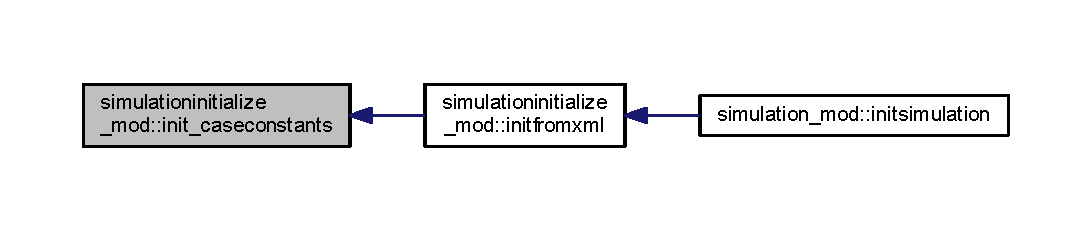
\includegraphics[width=350pt]{namespacesimulationinitialize__mod_ae41256ca5e72ebf27660ffdfe5c08e46_icgraph}
\end{center}
\end{figure}
\mbox{\Hypertarget{namespacesimulationinitialize__mod_a4909cc4cb57549e6eed3f69d6dfa30b5}\label{namespacesimulationinitialize__mod_a4909cc4cb57549e6eed3f69d6dfa30b5}} 
\index{simulationinitialize\+\_\+mod@{simulationinitialize\+\_\+mod}!init\+\_\+naming@{init\+\_\+naming}}
\index{init\+\_\+naming@{init\+\_\+naming}!simulationinitialize\+\_\+mod@{simulationinitialize\+\_\+mod}}
\subsubsection{\texorpdfstring{init\+\_\+naming()}{init\_naming()}}
{\footnotesize\ttfamily subroutine simulationinitialize\+\_\+mod\+::init\+\_\+naming (\begin{DoxyParamCaption}\item[{type(node), intent(in), pointer}]{case\+\_\+node }\end{DoxyParamCaption})\hspace{0.3cm}{\ttfamily [private]}}



naming xml parser routine. Reads the naming file(s), opens the file(s) and stores the naming conventions for input files 

\begin{DoxyAuthor}{Author}
Ricardo Birjukovs Canelas -\/ M\+A\+R\+E\+T\+EC 
\end{DoxyAuthor}

\begin{DoxyParams}[1]{Parameters}
\mbox{\tt in}  & {\em case\+\_\+node} & \\
\hline
\end{DoxyParams}


Definition at line 213 of file simulation\+Initialize.\+f90.


\begin{DoxyCode}
213     \textcolor{keywordtype}{type}(Node), \textcolor{keywordtype}{intent(in)}, \textcolor{keywordtype}{pointer} :: case\_node
214     \textcolor{keywordtype}{type}(Node), \textcolor{keywordtype}{pointer} :: naming\_node
215     \textcolor{keywordtype}{type}(Node), \textcolor{keywordtype}{pointer} :: temp
216     \textcolor{keywordtype}{type}(NodeList), \textcolor{keywordtype}{pointer} :: namingfileList
217     \textcolor{keywordtype}{type}(string) :: outext
218     \textcolor{keywordtype}{type}(string) :: tag, att\_name
219     \textcolor{keywordtype}{type}(string), \textcolor{keywordtype}{allocatable}, \textcolor{keywordtype}{dimension(:)} :: namingFilename
220     \textcolor{keywordtype}{integer} :: i
221 
222     tag=\textcolor{stringliteral}{"variableNaming"}    \textcolor{comment}{!the node we want}
223     \textcolor{keyword}{call }xmlreader%gotoNode(case\_node,naming\_node,tag,mandatory =.false.)
224     \textcolor{keywordflow}{if} (\textcolor{keyword}{associated}(naming\_node)) \textcolor{keywordflow}{then}
225         namingfilelist => getelementsbytagname(naming\_node, \textcolor{stringliteral}{"file"})       \textcolor{comment}{!searching for tags with the
       'namingfile' name}
226         \textcolor{keyword}{allocate}(namingfilename(getlength(namingfilelist)))
227         \textcolor{keywordflow}{do} i = 0, getlength(namingfilelist) - 1
228             temp => item(namingfilelist, i)
229             att\_name=\textcolor{stringliteral}{"name"}
230             \textcolor{keyword}{call }xmlreader%getLeafAttribute(temp,att\_name,namingfilename(i+1))
231 \textcolor{keywordflow}{        end do}
232         \textcolor{keyword}{call }globals%setNamingConventions(namingfilename)
233     \textcolor{keywordflow}{else}
234         outext=\textcolor{stringliteral}{'-->No naming files, assuming basic naming settings for variables from input files'}
235         \textcolor{keyword}{call }log%put(outext,.false.)
236 \textcolor{keywordflow}{    endif}
237 
\end{DoxyCode}
Here is the caller graph for this function\+:\nopagebreak
\begin{figure}[H]
\begin{center}
\leavevmode
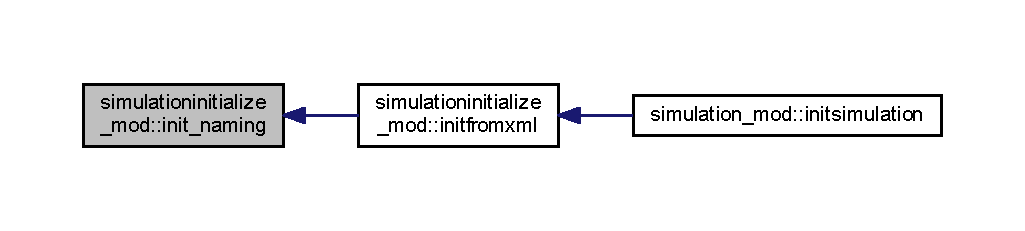
\includegraphics[width=350pt]{namespacesimulationinitialize__mod_a4909cc4cb57549e6eed3f69d6dfa30b5_icgraph}
\end{center}
\end{figure}
\mbox{\Hypertarget{namespacesimulationinitialize__mod_a0b32e8c950fc615198d1e47ba1d36cd6}\label{namespacesimulationinitialize__mod_a0b32e8c950fc615198d1e47ba1d36cd6}} 
\index{simulationinitialize\+\_\+mod@{simulationinitialize\+\_\+mod}!init\+\_\+parameters@{init\+\_\+parameters}}
\index{init\+\_\+parameters@{init\+\_\+parameters}!simulationinitialize\+\_\+mod@{simulationinitialize\+\_\+mod}}
\subsubsection{\texorpdfstring{init\+\_\+parameters()}{init\_parameters()}}
{\footnotesize\ttfamily subroutine simulationinitialize\+\_\+mod\+::init\+\_\+parameters (\begin{DoxyParamCaption}\item[{type(node), intent(in), pointer}]{execution\+\_\+node }\end{DoxyParamCaption})\hspace{0.3cm}{\ttfamily [private]}}



Private parameter parser routine. Builds the simulation parametric space from the input xml case file. 

\begin{DoxyAuthor}{Author}
Ricardo Birjukovs Canelas -\/ M\+A\+R\+E\+T\+EC 
\end{DoxyAuthor}

\begin{DoxyParams}[1]{Parameters}
\mbox{\tt in}  & {\em execution\+\_\+node} & \\
\hline
\end{DoxyParams}


Definition at line 558 of file simulation\+Initialize.\+f90.


\begin{DoxyCode}
558     \textcolor{keywordtype}{type}(Node), \textcolor{keywordtype}{intent(in)}, \textcolor{keywordtype}{pointer} :: execution\_node
559     \textcolor{keywordtype}{type}(string) :: outext
560     \textcolor{keywordtype}{type}(NodeList), \textcolor{keywordtype}{pointer} :: parameterList
561     \textcolor{keywordtype}{type}(Node), \textcolor{keywordtype}{pointer} :: parmt, parameters\_node
562     \textcolor{keywordtype}{integer} :: i
563     \textcolor{keywordtype}{type}(string) :: parmkey, parmvalue, tag, att\_name
564 
565     outext=\textcolor{stringliteral}{'-->Reading case parameters'}
566     \textcolor{keyword}{call }log%put(outext,.false.)
567 
568     tag=\textcolor{stringliteral}{"parameters"}    \textcolor{comment}{!the node we want}
569     \textcolor{keyword}{call }xmlreader%gotoNode(execution\_node,parameters\_node,tag)
570     parameterlist => getelementsbytagname(parameters\_node, \textcolor{stringliteral}{"parameter"})       \textcolor{comment}{!searching for tags with the
       'parameter' name}
571     \textcolor{keywordflow}{do} i = 0, getlength(parameterlist) - 1                          \textcolor{comment}{!extracting parameter tags one by one}
572         parmt => item(parameterlist, i)
573         att\_name=\textcolor{stringliteral}{"key"}
574         \textcolor{keyword}{call }xmlreader%getLeafAttribute(parmt,att\_name,parmkey)
575         att\_name=\textcolor{stringliteral}{"value"}
576         \textcolor{keyword}{call }xmlreader%getLeafAttribute(parmt,att\_name,parmvalue)
577         \textcolor{keyword}{call }globals%Parameters%setParam(parmkey,parmvalue)
578 \textcolor{keywordflow}{    end do}
579     \textcolor{keyword}{call }globals%Parameters%check()
580     \textcolor{keyword}{call }globals%Parameters%print()
581     
582     \textcolor{keyword}{call }globals%setTimeDate()
583     \textcolor{keyword}{call }globals%SimTime%print()
584 
\end{DoxyCode}
Here is the caller graph for this function\+:\nopagebreak
\begin{figure}[H]
\begin{center}
\leavevmode
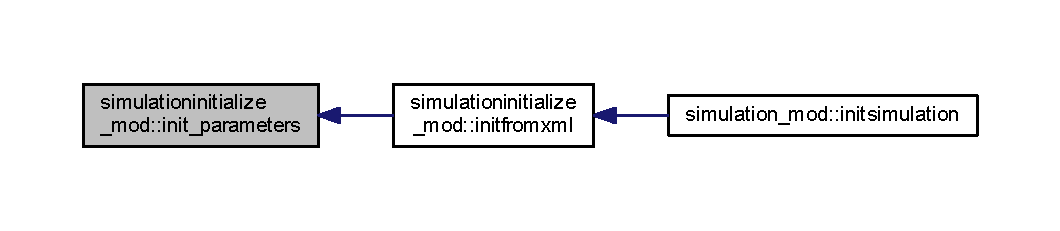
\includegraphics[width=350pt]{namespacesimulationinitialize__mod_a0b32e8c950fc615198d1e47ba1d36cd6_icgraph}
\end{center}
\end{figure}
\mbox{\Hypertarget{namespacesimulationinitialize__mod_a532cb4960e93dc27cff5dc2e04afe070}\label{namespacesimulationinitialize__mod_a532cb4960e93dc27cff5dc2e04afe070}} 
\index{simulationinitialize\+\_\+mod@{simulationinitialize\+\_\+mod}!init\+\_\+properties@{init\+\_\+properties}}
\index{init\+\_\+properties@{init\+\_\+properties}!simulationinitialize\+\_\+mod@{simulationinitialize\+\_\+mod}}
\subsubsection{\texorpdfstring{init\+\_\+properties()}{init\_properties()}}
{\footnotesize\ttfamily subroutine simulationinitialize\+\_\+mod\+::init\+\_\+properties (\begin{DoxyParamCaption}\item[{type(node), intent(in), pointer}]{case\+\_\+node }\end{DoxyParamCaption})\hspace{0.3cm}{\ttfamily [private]}}



Private property xml parser routine. Reads the properties tab from the xml file and links these to the corresponding source. 

\begin{DoxyAuthor}{Author}
Ricardo Birjukovs Canelas -\/ M\+A\+R\+E\+T\+EC 
\end{DoxyAuthor}

\begin{DoxyParams}[1]{Parameters}
\mbox{\tt in}  & {\em case\+\_\+node} & \\
\hline
\end{DoxyParams}


Definition at line 125 of file simulation\+Initialize.\+f90.


\begin{DoxyCode}
125     \textcolor{keywordtype}{type}(Node), \textcolor{keywordtype}{intent(in)}, \textcolor{keywordtype}{pointer} :: case\_node
126 
127     \textcolor{keywordtype}{type}(Node), \textcolor{keywordtype}{pointer} :: props\_node
128     \textcolor{keywordtype}{type}(string) :: outext
129     \textcolor{keywordtype}{type}(string) :: tag, att\_name
130 
131     tag=\textcolor{stringliteral}{"sourceTypes"}    \textcolor{comment}{!the node we want}
132     \textcolor{keyword}{call }xmlreader%gotoNode(case\_node,props\_node,tag,mandatory =.false.)
133     \textcolor{keywordflow}{if} (\textcolor{keyword}{associated}(props\_node)) \textcolor{keywordflow}{then}
134         tag=\textcolor{stringliteral}{"file"}
135         att\_name=\textcolor{stringliteral}{"name"}
136         \textcolor{keyword}{call }xmlreader%getNodeAttribute(props\_node, tag, att\_name, globals%Names%propsxmlfilename) \textcolor{comment}{!getting
       the file name from that tag}
137         outext=\textcolor{stringliteral}{'-->Properties to link to Sources found at '}//globals%Names%propsxmlfilename
138         \textcolor{keyword}{call }log%put(outext,.false.)
139         tag=\textcolor{stringliteral}{"types"}
140         \textcolor{keyword}{call }xmlreader%gotoNode(props\_node,props\_node,tag) \textcolor{comment}{!getting the links node}
141         \textcolor{keyword}{call }linkpropertysources(props\_node)          \textcolor{comment}{!calling the property linker}
142     \textcolor{keywordflow}{else}
143         outext=\textcolor{stringliteral}{'-->No properties to link to Sources, assuming pure Lagrangian tracers'}
144         \textcolor{keyword}{call }log%put(outext,.false.)
145 \textcolor{keywordflow}{    endif}
146 
\end{DoxyCode}
Here is the call graph for this function\+:\nopagebreak
\begin{figure}[H]
\begin{center}
\leavevmode
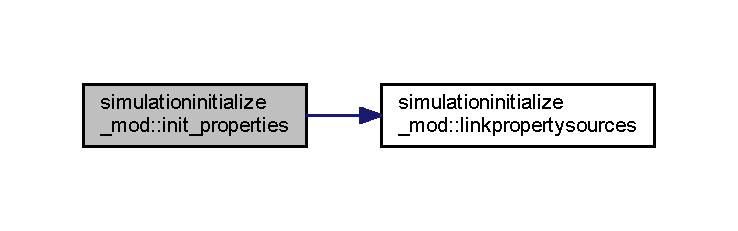
\includegraphics[width=350pt]{namespacesimulationinitialize__mod_a532cb4960e93dc27cff5dc2e04afe070_cgraph}
\end{center}
\end{figure}
Here is the caller graph for this function\+:\nopagebreak
\begin{figure}[H]
\begin{center}
\leavevmode
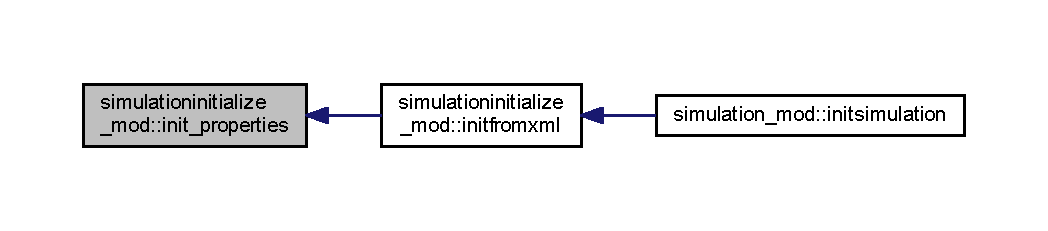
\includegraphics[width=350pt]{namespacesimulationinitialize__mod_a532cb4960e93dc27cff5dc2e04afe070_icgraph}
\end{center}
\end{figure}
\mbox{\Hypertarget{namespacesimulationinitialize__mod_af6b2508d52e9e29aeb6e7dfbabd88e8d}\label{namespacesimulationinitialize__mod_af6b2508d52e9e29aeb6e7dfbabd88e8d}} 
\index{simulationinitialize\+\_\+mod@{simulationinitialize\+\_\+mod}!init\+\_\+simdefs@{init\+\_\+simdefs}}
\index{init\+\_\+simdefs@{init\+\_\+simdefs}!simulationinitialize\+\_\+mod@{simulationinitialize\+\_\+mod}}
\subsubsection{\texorpdfstring{init\+\_\+simdefs()}{init\_simdefs()}}
{\footnotesize\ttfamily subroutine simulationinitialize\+\_\+mod\+::init\+\_\+simdefs (\begin{DoxyParamCaption}\item[{type(node), intent(in), pointer}]{case\+\_\+node }\end{DoxyParamCaption})\hspace{0.3cm}{\ttfamily [private]}}



Private simulation definitions parser routine. Builds the simulation geometric space from the input xml case file. 

\begin{DoxyAuthor}{Author}
Ricardo Birjukovs Canelas -\/ M\+A\+R\+E\+T\+EC 
\end{DoxyAuthor}

\begin{DoxyParams}[1]{Parameters}
\mbox{\tt in}  & {\em case\+\_\+node} & \\
\hline
\end{DoxyParams}


Definition at line 450 of file simulation\+Initialize.\+f90.


\begin{DoxyCode}
450     \textcolor{keywordtype}{type}(Node), \textcolor{keywordtype}{intent(in)}, \textcolor{keywordtype}{pointer} :: case\_node
451     \textcolor{keywordtype}{type}(NodeList), \textcolor{keywordtype}{pointer} :: defsList
452     \textcolor{keywordtype}{type}(Node), \textcolor{keywordtype}{pointer} :: simdefs\_node
453     \textcolor{keywordtype}{type}(string) :: outext
454     \textcolor{keywordtype}{integer} :: i
455     \textcolor{keywordtype}{type}(string) :: pts(2), tag, att\_name, att\_val
456     \textcolor{keywordtype}{type}(vector) :: coords
457     \textcolor{keywordtype}{logical} :: read\_flag
458 
459     read\_flag = .false.
460     coords = 0.0
461     outext=\textcolor{stringliteral}{'-->Reading case simulation definitions'}
462     \textcolor{keyword}{call }log%put(outext,.false.)
463 
464     tag=\textcolor{stringliteral}{"simulation"}    \textcolor{comment}{!the node we want}
465     \textcolor{keyword}{call }xmlreader%gotoNode(case\_node,simdefs\_node,tag)
466     tag=\textcolor{stringliteral}{"resolution"}
467     att\_name=\textcolor{stringliteral}{"dp"}
468     \textcolor{keyword}{call }xmlreader%getNodeAttribute(simdefs\_node, tag, att\_name, att\_val, read\_flag, .false.)
469     \textcolor{keywordflow}{if} (read\_flag) \textcolor{keywordflow}{then}
470         coords = att\_val%to\_number(kind=1.\_r4p)
471     \textcolor{keywordflow}{else}
472         \textcolor{keyword}{call }xmlreader%getNodeVector(simdefs\_node, tag, coords)
473 \textcolor{keywordflow}{    end if}
474     \textcolor{keyword}{call }globals%SimDefs%setdp(coords)
475     tag=\textcolor{stringliteral}{"timestep"}
476     att\_name=\textcolor{stringliteral}{"dt"}
477     \textcolor{keyword}{call }xmlreader%getNodeAttribute(simdefs\_node, tag, att\_name, att\_val)
478     \textcolor{keyword}{call }globals%SimDefs%setdt(att\_val)
479     \textcolor{keyword}{call }globals%Constants%setSmallDt(globals%SimDefs%dt)
480     pts=(/ \textcolor{stringliteral}{'BoundingBoxMin'}, \textcolor{stringliteral}{'BoundingBoxMax'}/) \textcolor{comment}{!strings to search for}
481     \textcolor{keywordflow}{do} i=1, \textcolor{keyword}{size}(pts)
482         \textcolor{keyword}{call }xmlreader%getNodeVector(simdefs\_node, pts(i), coords)
483         \textcolor{keyword}{call }globals%SimDefs%setboundingbox(pts(i), coords)
484 \textcolor{keywordflow}{    enddo}
485     \textcolor{keyword}{call }globals%SimDefs%print()
486 
\end{DoxyCode}
Here is the caller graph for this function\+:\nopagebreak
\begin{figure}[H]
\begin{center}
\leavevmode
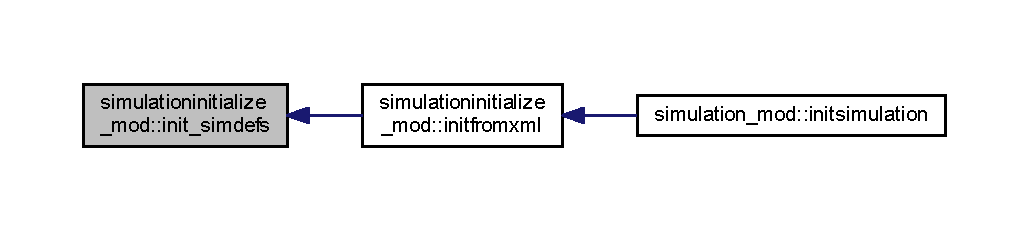
\includegraphics[width=350pt]{namespacesimulationinitialize__mod_af6b2508d52e9e29aeb6e7dfbabd88e8d_icgraph}
\end{center}
\end{figure}
\mbox{\Hypertarget{namespacesimulationinitialize__mod_acaa6b217159e3a10e7db04dd7b0e4058}\label{namespacesimulationinitialize__mod_acaa6b217159e3a10e7db04dd7b0e4058}} 
\index{simulationinitialize\+\_\+mod@{simulationinitialize\+\_\+mod}!init\+\_\+sources@{init\+\_\+sources}}
\index{init\+\_\+sources@{init\+\_\+sources}!simulationinitialize\+\_\+mod@{simulationinitialize\+\_\+mod}}
\subsubsection{\texorpdfstring{init\+\_\+sources()}{init\_sources()}}
{\footnotesize\ttfamily subroutine simulationinitialize\+\_\+mod\+::init\+\_\+sources (\begin{DoxyParamCaption}\item[{type(node), intent(in), pointer}]{case\+\_\+node }\end{DoxyParamCaption})\hspace{0.3cm}{\ttfamily [private]}}



Private source definitions parser routine. Builds the tracer sources from the input xml case file. 

\begin{DoxyAuthor}{Author}
Ricardo Birjukovs Canelas -\/ M\+A\+R\+E\+T\+EC 
\end{DoxyAuthor}

\begin{DoxyParams}[1]{Parameters}
\mbox{\tt in}  & {\em case\+\_\+node} & \\
\hline
\end{DoxyParams}


Definition at line 299 of file simulation\+Initialize.\+f90.


\begin{DoxyCode}
299     \textcolor{keywordtype}{implicit none}
300     \textcolor{keywordtype}{type}(Node), \textcolor{keywordtype}{intent(in)}, \textcolor{keywordtype}{pointer} :: case\_node
301     \textcolor{keywordtype}{type}(string) :: outext
302     \textcolor{keywordtype}{type}(NodeList), \textcolor{keywordtype}{pointer} :: sourceList
303     \textcolor{keywordtype}{type}(NodeList), \textcolor{keywordtype}{pointer} :: sourceChildren
304     \textcolor{keywordtype}{type}(NodeList), \textcolor{keywordtype}{pointer} :: activeList
305     \textcolor{keywordtype}{type}(Node), \textcolor{keywordtype}{pointer} :: activeIntervalNode
306     \textcolor{keywordtype}{type}(Node), \textcolor{keywordtype}{pointer} :: sourcedef
307     \textcolor{keywordtype}{type}(Node), \textcolor{keywordtype}{pointer} :: source\_node
308     \textcolor{keywordtype}{type}(Node), \textcolor{keywordtype}{pointer} :: source\_detail
309     \textcolor{keywordtype}{type}(Node), \textcolor{keywordtype}{pointer} :: source\_ratefile, ratefileLeaf
310     \textcolor{keywordtype}{type}(Node), \textcolor{keywordtype}{pointer} :: source\_posifile, posifileLeaf
311     \textcolor{keywordtype}{integer} :: i, j, k
312     \textcolor{keywordtype}{logical} :: readflag
313     \textcolor{keywordtype}{integer} :: id
314     \textcolor{keywordtype}{type}(string) :: name, source\_geometry, tag, att\_name, att\_val, rate\_file, posi\_file
315     \textcolor{keywordtype}{real(prec)} :: emitting\_rate, rateScale, start, finish, temp
316     \textcolor{keywordtype}{logical} :: emitting\_fixed, posi\_fixed, rateRead
317     \textcolor{keywordtype}{class}(shape), \textcolor{keywordtype}{allocatable} :: source\_shape
318     \textcolor{keywordtype}{type}(vector) :: res
319     \textcolor{keywordtype}{real(prec)}, \textcolor{keywordtype}{dimension(:,:)}, \textcolor{keywordtype}{allocatable} :: activeTimes
320 
321     ratescale = 1.0
322     res = 0.0    
323     readflag = .false.
324     outext=\textcolor{stringliteral}{'-->Reading case Sources'}
325     \textcolor{keyword}{call }log%put(outext,.false.)
326     tag=\textcolor{stringliteral}{"sourceDefinitions"}    \textcolor{comment}{!the node we want}
327     \textcolor{keyword}{call }xmlreader%gotoNode(case\_node,sourcedef,tag)
328     sourcelist => getelementsbytagname(sourcedef, \textcolor{stringliteral}{"source"})
329     \textcolor{comment}{!allocating the temporary source objects}
330     \textcolor{keyword}{call }tempsources%initialize(getlength(sourcelist))
331 
332     \textcolor{keywordflow}{do} j = 0, getlength(sourcelist) - 1
333         rate\_file = notset
334         rateread = .false.
335         posi\_file = notset
336         posi\_fixed = .true.
337         source\_node => item(sourcelist,j)
338         tag=\textcolor{stringliteral}{"setsource"}
339         att\_name=\textcolor{stringliteral}{"id"}
340         \textcolor{keyword}{call }xmlreader%getNodeAttribute(source\_node, tag, att\_name, att\_val)
341         id=att\_val%to\_number(kind=1\_i1p)
342         att\_name=\textcolor{stringliteral}{"name"}
343         \textcolor{keyword}{call }xmlreader%getNodeAttribute(source\_node, tag, att\_name, name)
344         \textcolor{comment}{!reading possible custom resolution}
345         tag=\textcolor{stringliteral}{"resolution"}
346         att\_name=\textcolor{stringliteral}{"dp"}
347         \textcolor{keyword}{call }xmlreader%getNodeAttribute(source\_node, tag, att\_name, att\_val, readflag, .false.)
348         \textcolor{keywordflow}{if} (readflag) \textcolor{keywordflow}{then}
349             res = att\_val%to\_number(kind=1.\_r4p)
350         \textcolor{keywordflow}{else}
351             \textcolor{keyword}{call }xmlreader%getNodeVector(source\_node, tag, res, readflag, .false.)
352             \textcolor{keywordflow}{if} (.not.readflag) res = 0.0
353 \textcolor{keywordflow}{        end if}
354         \textcolor{comment}{!reading emission rate, need to check for options}
355         readflag = .false.
356         tag=\textcolor{stringliteral}{"rate\_dt"}
357         att\_name=\textcolor{stringliteral}{"value"}
358         \textcolor{keyword}{call }xmlreader%getNodeAttribute(source\_node, tag, att\_name, att\_val, readflag, .false.)
359         \textcolor{keywordflow}{if} (readflag) \textcolor{keywordflow}{then}
360             rateread = .true.
361             emitting\_rate = 1.0/(att\_val%to\_number(kind=1.\_r4p)*globals%SimDefs%dt)
362             emitting\_fixed = .true.
363 \textcolor{keywordflow}{        end if}
364         tag=\textcolor{stringliteral}{"rate"}
365         att\_name=\textcolor{stringliteral}{"value"}
366         \textcolor{keyword}{call }xmlreader%getNodeAttribute(source\_node, tag, att\_name, att\_val, readflag, .false.)
367         \textcolor{keywordflow}{if} (readflag) \textcolor{keywordflow}{then}
368             rateread = .true.
369             emitting\_rate = att\_val%to\_number(kind=1.\_r4p)
370             emitting\_fixed = .true.
371 \textcolor{keywordflow}{        end if}
372         tag=\textcolor{stringliteral}{"rateTimeSeries"}
373         \textcolor{keyword}{call }xmlreader%gotoNode(source\_node, source\_ratefile, tag, mandatory =.false.)
374         \textcolor{keywordflow}{if} (\textcolor{keyword}{associated}(source\_ratefile)) \textcolor{keywordflow}{then}
375             tag = \textcolor{stringliteral}{"file"}
376             \textcolor{keyword}{call }xmlreader%gotoNode(source\_ratefile, ratefileleaf, tag)
377             att\_name=\textcolor{stringliteral}{"name"}
378             \textcolor{keyword}{call }xmlreader%getLeafAttribute(ratefileleaf, att\_name, att\_val)
379             rateread = .true.
380             rate\_file = att\_val
381             emitting\_fixed = .false.
382             tag = \textcolor{stringliteral}{"scale"}
383             att\_name=\textcolor{stringliteral}{"value"}
384             \textcolor{keyword}{call }xmlreader%getNodeAttribute(source\_ratefile, tag, att\_name, att\_val, readflag, mandatory = 
      .false.)            
385             \textcolor{keywordflow}{if} (readflag) \textcolor{keywordflow}{then}
386                 ratescale = att\_val%to\_number(kind=1.\_r4p)
387 \textcolor{keywordflow}{            end if}
388 \textcolor{keywordflow}{        end if}
389         \textcolor{keywordflow}{if} (.not.rateread) \textcolor{keywordflow}{then}
390             outext=\textcolor{stringliteral}{'-->Source '}//name//\textcolor{stringliteral}{' (id = '}//id// \textcolor{stringliteral}{') doesn'}\textcolor{stringliteral}{'t have emission rate information. Possible
       options are [rate\_dt, rate, rate\_file]. Stoping'}
391             \textcolor{keyword}{call }log%put(outext)
392             stop
393 \textcolor{keywordflow}{        end if}
394         \textcolor{comment}{!reading variable position tags, if any}
395         tag=\textcolor{stringliteral}{"positionTimeSeries"}
396         \textcolor{keyword}{call }xmlreader%gotoNode(source\_node, source\_posifile, tag, mandatory =.false.)
397         \textcolor{keywordflow}{if} (\textcolor{keyword}{associated}(source\_posifile)) \textcolor{keywordflow}{then}
398             tag = \textcolor{stringliteral}{"file"}
399             \textcolor{keyword}{call }xmlreader%gotoNode(source\_posifile, posifileleaf, tag)
400             att\_name=\textcolor{stringliteral}{"name"}
401             \textcolor{keyword}{call }xmlreader%getLeafAttribute(posifileleaf, att\_name, att\_val)
402             posi\_file = att\_val
403             posi\_fixed = .false.
404 \textcolor{keywordflow}{        end if}
405         \textcolor{comment}{!Possible list of active intervals, and these might be in absolute dates or relative to sim time}
406         activelist => getelementsbytagname(source\_node, \textcolor{stringliteral}{"active"})
407         \textcolor{keyword}{allocate}(activetimes(getlength(activelist),2))
408         \textcolor{keywordflow}{do} k = 0, getlength(activelist) - 1
409             activeintervalnode => item(activelist, k)
410             att\_name=\textcolor{stringliteral}{"start"}
411             \textcolor{keyword}{call }xmlreader%getLeafAttribute(activeintervalnode,att\_name,att\_val)
412             temp = utils%getRelativeTimeFromString(att\_val, globals%SimTime%StartDate)
413             activetimes(k+1,1) = temp
414             att\_name=\textcolor{stringliteral}{"end"}
415             \textcolor{keyword}{call }xmlreader%getLeafAttribute(activeintervalnode,att\_name,att\_val)
416             \textcolor{keywordflow}{if} (att\_val == \textcolor{stringliteral}{'end'}) \textcolor{keywordflow}{then}
417                 temp = globals%Parameters%TimeMax
418             \textcolor{keywordflow}{else}
419                 temp = utils%getRelativeTimeFromString(att\_val, globals%SimTime%StartDate)
420 \textcolor{keywordflow}{            end if}
421             activetimes(k+1,2) = temp
422 \textcolor{keywordflow}{        end do}
423         \textcolor{comment}{!now we need to find out the geometry of the source and read accordingly}
424         sourcechildren => getchildnodes(source\_node) \textcolor{comment}{!getting all of the nodes bellow the main source node
       (all of it's private info)}
425         \textcolor{keywordflow}{do} i=0, getlength(sourcechildren)-1
426             source\_detail => item(sourcechildren,i) \textcolor{comment}{!grabing a node}
427             source\_geometry = getlocalname(source\_detail)  \textcolor{comment}{!finding its name}
428             \textcolor{keywordflow}{if} (geometry%inlist(source\_geometry)) \textcolor{keywordflow}{then}  \textcolor{comment}{!if the node is a valid geometry name}
429                 \textcolor{keyword}{call }geometry%allocateShape(source\_geometry,source\_shape)                
430                 \textcolor{keyword}{call }read\_xml\_geometry(source\_node,source\_detail,source\_shape)
431                 \textcolor{keywordflow}{exit}
432 \textcolor{keywordflow}{            end if}
433 \textcolor{keywordflow}{        end do}
434         \textcolor{comment}{!initializing Source j}
435         \textcolor{keyword}{call }tempsources%src(j+1)%initialize(id, name, emitting\_rate, emitting\_fixed, rate\_file, ratescale,
       posi\_fixed, posi\_file, activetimes, source\_geometry, source\_shape, res)
436 
437         \textcolor{keyword}{deallocate}(source\_shape)
438         \textcolor{keyword}{deallocate}(activetimes)
439 \textcolor{keywordflow}{    enddo}
440 
\end{DoxyCode}
Here is the call graph for this function\+:\nopagebreak
\begin{figure}[H]
\begin{center}
\leavevmode
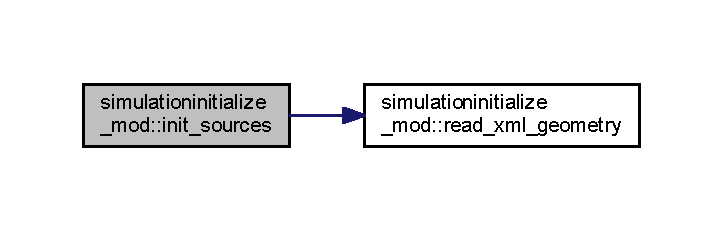
\includegraphics[width=347pt]{namespacesimulationinitialize__mod_acaa6b217159e3a10e7db04dd7b0e4058_cgraph}
\end{center}
\end{figure}
Here is the caller graph for this function\+:\nopagebreak
\begin{figure}[H]
\begin{center}
\leavevmode
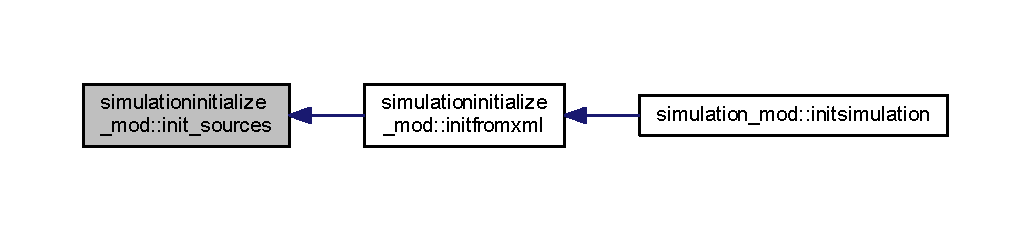
\includegraphics[width=350pt]{namespacesimulationinitialize__mod_acaa6b217159e3a10e7db04dd7b0e4058_icgraph}
\end{center}
\end{figure}
\mbox{\Hypertarget{namespacesimulationinitialize__mod_ada0310fe0d45fa2eec30deaf3ad25ba7}\label{namespacesimulationinitialize__mod_ada0310fe0d45fa2eec30deaf3ad25ba7}} 
\index{simulationinitialize\+\_\+mod@{simulationinitialize\+\_\+mod}!initfromxml@{initfromxml}}
\index{initfromxml@{initfromxml}!simulationinitialize\+\_\+mod@{simulationinitialize\+\_\+mod}}
\subsubsection{\texorpdfstring{initfromxml()}{initfromxml()}}
{\footnotesize\ttfamily subroutine, public simulationinitialize\+\_\+mod\+::initfromxml (\begin{DoxyParamCaption}\item[{type(string), intent(in)}]{xmlfilename }\end{DoxyParamCaption})}



Public xml parser routine. Builds the simulation space from the input xml case file. 

\begin{DoxyAuthor}{Author}
Ricardo Birjukovs Canelas -\/ M\+A\+R\+E\+T\+EC 
\end{DoxyAuthor}

\begin{DoxyParams}[1]{Parameters}
\mbox{\tt in}  & {\em xmlfilename} & \\
\hline
\mbox{\tt in}  & {\em xmlfilename} & .xml file name \\
\hline
\end{DoxyParams}


Definition at line 594 of file simulation\+Initialize.\+f90.


\begin{DoxyCode}
594     \textcolor{keywordtype}{implicit none}
595     \textcolor{keywordtype}{type}(string), \textcolor{keywordtype}{intent(in)} :: xmlfilename
596     \textcolor{keywordtype}{type}(string) :: outext, tag
597     \textcolor{keywordtype}{type}(Node), \textcolor{keywordtype}{pointer} :: xmldoc
598     \textcolor{keywordtype}{type}(Node), \textcolor{keywordtype}{pointer} :: case\_node
599     \textcolor{keywordtype}{type}(Node), \textcolor{keywordtype}{pointer} :: execution\_node
600 
601     \textcolor{keyword}{call }xmlreader%getFile(xmldoc,xmlfilename)
602     globals%Names%mainxmlfilename = xmlfilename
603     globals%Names%casename = xmlfilename%basename(extension=\textcolor{stringliteral}{'.xml'})
604     outext=\textcolor{stringliteral}{'->Case name is '}//globals%Names%casename
605     \textcolor{keyword}{call }log%put(outext)
606     globals%Names%inputsXmlFilename = globals%Names%outpath//xmlfilename%basename(extension=\textcolor{stringliteral}{'.xml'})//\textcolor{stringliteral}{
      '\_inputs.xml'}
607     outext=\textcolor{stringliteral}{'->Input files index file name is '}//globals%Names%inputsXmlFilename
608     \textcolor{keyword}{call }log%put(outext)
609 
610     tag=\textcolor{stringliteral}{"case"}          \textcolor{comment}{!base document node}
611     \textcolor{keyword}{call }xmlreader%gotoNode(xmldoc,execution\_node,tag)
612     tag=\textcolor{stringliteral}{"execution"}     \textcolor{comment}{!finding execution node}
613     \textcolor{keyword}{call }xmlreader%gotoNode(execution\_node,execution\_node,tag)
614     tag=\textcolor{stringliteral}{"case"}          \textcolor{comment}{!base document node}
615     \textcolor{keyword}{call }xmlreader%gotoNode(xmldoc,case\_node,tag)
616     tag=\textcolor{stringliteral}{"caseDefinitions"}     \textcolor{comment}{!finding execution node}
617     \textcolor{keyword}{call }xmlreader%gotoNode(case\_node,case\_node,tag)
618 
619     \textcolor{comment}{! building the simulation basic structures according to the case definition file}
620     \textcolor{comment}{! every other structure in the simulation is built from these, i.e., not defined by the user directly}
621     \textcolor{keyword}{call }init\_parameters(execution\_node)
622     \textcolor{keyword}{call }init\_naming(execution\_node)
623     \textcolor{keyword}{call }setoutputfields(execution\_node)
624     \textcolor{keyword}{call }init\_caseconstants(case\_node)
625     \textcolor{keyword}{call }init\_simdefs(case\_node)
626     \textcolor{keyword}{call }init\_sources(case\_node)
627     \textcolor{keyword}{call }init\_properties(case\_node)    
628 
629     \textcolor{comment}{!setting the number of blocks to the correct ammount of selected threads}
630     globals%SimDefs%numblocks = globals%Parameters%numOPMthreads
631 
632     \textcolor{keyword}{call }xmlreader%closeFile(xmldoc)
633 
\end{DoxyCode}
Here is the call graph for this function\+:\nopagebreak
\begin{figure}[H]
\begin{center}
\leavevmode
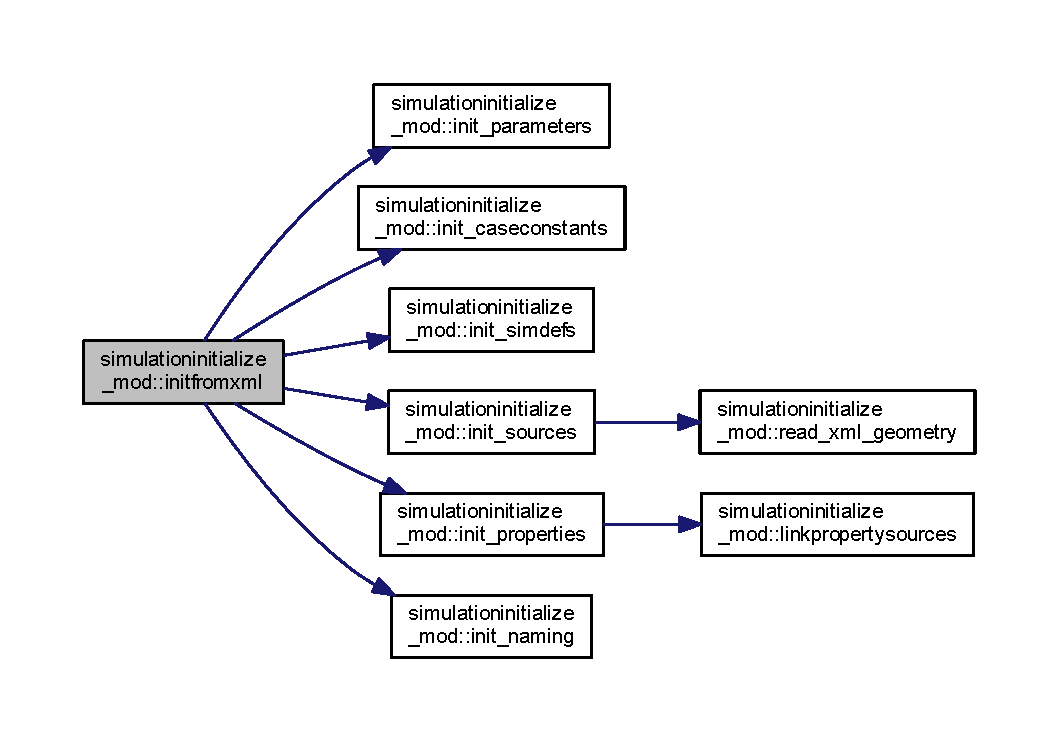
\includegraphics[width=350pt]{namespacesimulationinitialize__mod_ada0310fe0d45fa2eec30deaf3ad25ba7_cgraph}
\end{center}
\end{figure}
Here is the caller graph for this function\+:\nopagebreak
\begin{figure}[H]
\begin{center}
\leavevmode
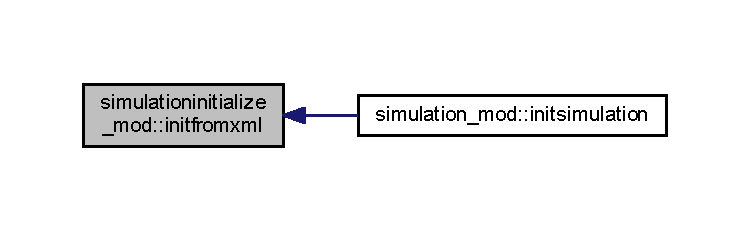
\includegraphics[width=350pt]{namespacesimulationinitialize__mod_ada0310fe0d45fa2eec30deaf3ad25ba7_icgraph}
\end{center}
\end{figure}
\mbox{\Hypertarget{namespacesimulationinitialize__mod_aa4c1099b84c9901ab1286a3796a54f71}\label{namespacesimulationinitialize__mod_aa4c1099b84c9901ab1286a3796a54f71}} 
\index{simulationinitialize\+\_\+mod@{simulationinitialize\+\_\+mod}!linkpropertysources@{linkpropertysources}}
\index{linkpropertysources@{linkpropertysources}!simulationinitialize\+\_\+mod@{simulationinitialize\+\_\+mod}}
\subsubsection{\texorpdfstring{linkpropertysources()}{linkpropertysources()}}
{\footnotesize\ttfamily subroutine simulationinitialize\+\_\+mod\+::linkpropertysources (\begin{DoxyParamCaption}\item[{type(node), intent(in), pointer}]{links\+Node }\end{DoxyParamCaption})\hspace{0.3cm}{\ttfamily [private]}}



Private property xml parser routine. Reads the properties tab from the xml file and links these to the corresponding Source. 

\begin{DoxyAuthor}{Author}
Ricardo Birjukovs Canelas -\/ M\+A\+R\+E\+T\+EC 
\end{DoxyAuthor}

\begin{DoxyParams}[1]{Parameters}
\mbox{\tt in}  & {\em links\+Node} & \\
\hline
\end{DoxyParams}


Definition at line 47 of file simulation\+Initialize.\+f90.


\begin{DoxyCode}
47     \textcolor{keywordtype}{type}(Node), \textcolor{keywordtype}{intent(in)}, \textcolor{keywordtype}{pointer} :: linksNode
48     \textcolor{keywordtype}{type}(NodeList), \textcolor{keywordtype}{pointer} :: linkList
49     \textcolor{keywordtype}{type}(Node), \textcolor{keywordtype}{pointer} :: anode
50     \textcolor{keywordtype}{type}(Node), \textcolor{keywordtype}{pointer} :: aProp
51     \textcolor{keywordtype}{type}(Node), \textcolor{keywordtype}{pointer} :: xmlProps
52     \textcolor{keywordtype}{type}(NodeList), \textcolor{keywordtype}{pointer} :: propertyList
53     \textcolor{keywordtype}{type}(string) :: xmlfilename, outext
54     \textcolor{keywordtype}{integer} :: i, p, j
55     \textcolor{keywordtype}{type}(string) :: att\_name, att\_val, tag, propKey, propValue
56     \textcolor{keywordtype}{type}(string) :: sourceid, sourcetype, sourceprop
57 
58     linklist => getelementsbytagname(linksnode, \textcolor{stringliteral}{"type"})
59     \textcolor{keywordflow}{do} i = 0, getlength(linklist) - 1
60         anode => item(linklist,i)
61         att\_name=\textcolor{stringliteral}{"source"}
62         \textcolor{keyword}{call }xmlreader%getLeafAttribute(anode,att\_name,sourceid)
63         att\_name=\textcolor{stringliteral}{"type"}
64         \textcolor{keyword}{call }xmlreader%getLeafAttribute(anode,att\_name,sourcetype)
65         att\_name=\textcolor{stringliteral}{"property"}
66         \textcolor{keyword}{call }xmlreader%getLeafAttribute(anode,att\_name,sourceprop)
67         \textcolor{comment}{!find the source and save the type and property name}
68         \textcolor{keyword}{call }tempsources%setPropertyNames(sourceid,sourcetype,sourceprop)
69 \textcolor{keywordflow}{    enddo}
70 
71     \textcolor{comment}{!parse the properties file}
72     xmlfilename = globals%Names%propsxmlfilename
73     \textcolor{keyword}{call }xmlreader%getFile(xmlprops,xmlfilename)
74 
75     \textcolor{comment}{!Go to the materials node}
76     tag = \textcolor{stringliteral}{"materials"}
77     \textcolor{keyword}{call }xmlreader%gotoNode(xmlprops,xmlprops,tag)
78 
79     \textcolor{comment}{!find and set the actual atributes of the properties}
80     att\_name=\textcolor{stringliteral}{"value"}
81     \textcolor{keywordflow}{do} i = 1, \textcolor{keyword}{size}(tempsources%src)
82         tag = tempsources%src(i)%prop%propertyType
83         \textcolor{keywordflow}{if} (tag .ne. \textcolor{stringliteral}{'base'}) \textcolor{keywordflow}{then}
84             \textcolor{keyword}{call }xmlreader%gotoNode(xmlprops,anode,tag) \textcolor{comment}{!finding the material type node}
85             tag = tempsources%src(i)%prop%propertySubType
86             \textcolor{keyword}{call }xmlreader%gotoNode(anode,anode,tag)     \textcolor{comment}{!finding the actual material node}
87             propertylist => getelementsbytagname(anode, \textcolor{stringliteral}{"property"})        \textcolor{comment}{!searching for tags with the
       'property' name}
88             \textcolor{keyword}{call }tempsources%src(i)%setPropertyNumber(getlength(propertylist))
89             \textcolor{keywordflow}{do} j = 0, getlength(propertylist) - 1                          \textcolor{comment}{!extracting property tags one by
       one}
90                 aprop => item(propertylist, j)
91                 att\_name=\textcolor{stringliteral}{"key"}
92                 \textcolor{keyword}{call }xmlreader%getLeafAttribute(aprop,att\_name,propkey)
93                 att\_name=\textcolor{stringliteral}{"value"}
94                 \textcolor{keyword}{call }xmlreader%getLeafAttribute(aprop,att\_name,propvalue)
95                 \textcolor{keyword}{call }tempsources%src(i)%setPropertyAtribute(j+1, propkey, propvalue)
96 \textcolor{keywordflow}{            end do}
97             tag = \textcolor{stringliteral}{'particulate'}
98             att\_name=\textcolor{stringliteral}{"value"}
99             \textcolor{keyword}{call }xmlreader%getNodeAttribute(anode, tag, att\_name, att\_val)
100             \textcolor{keyword}{call }tempsources%src(i)%setPropertyBaseAtribute(tag, att\_val)
101             tag = \textcolor{stringliteral}{'density'}
102             \textcolor{keyword}{call }xmlreader%getNodeAttribute(anode, tag, att\_name, att\_val)
103             \textcolor{keyword}{call }tempsources%src(i)%setPropertyBaseAtribute(tag, att\_val)
104             tag = \textcolor{stringliteral}{'radius'}
105             \textcolor{keyword}{call }xmlreader%getNodeAttribute(anode, tag, att\_name, att\_val)
106             \textcolor{keyword}{call }tempsources%src(i)%setPropertyBaseAtribute(tag, att\_val)           
107 \textcolor{keywordflow}{        end if}
108 \textcolor{keywordflow}{    end do}
109     outext=\textcolor{stringliteral}{'-->Sources properties are set'}
110     \textcolor{keyword}{call }log%put(outext,.false.)
111 
112     \textcolor{keyword}{call }xmlreader%closeFile(xmlprops)
113 
\end{DoxyCode}
Here is the caller graph for this function\+:\nopagebreak
\begin{figure}[H]
\begin{center}
\leavevmode
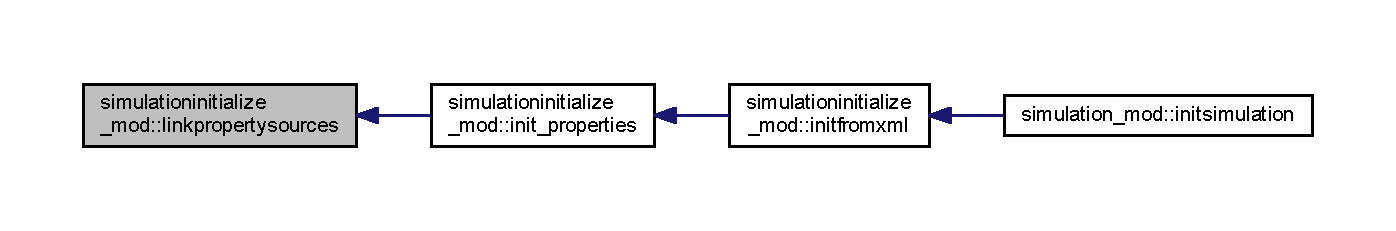
\includegraphics[width=350pt]{namespacesimulationinitialize__mod_aa4c1099b84c9901ab1286a3796a54f71_icgraph}
\end{center}
\end{figure}
\mbox{\Hypertarget{namespacesimulationinitialize__mod_ab65ac868a57f2cc124ec29f87a239424}\label{namespacesimulationinitialize__mod_ab65ac868a57f2cc124ec29f87a239424}} 
\index{simulationinitialize\+\_\+mod@{simulationinitialize\+\_\+mod}!read\+\_\+xml\+\_\+geometry@{read\+\_\+xml\+\_\+geometry}}
\index{read\+\_\+xml\+\_\+geometry@{read\+\_\+xml\+\_\+geometry}!simulationinitialize\+\_\+mod@{simulationinitialize\+\_\+mod}}
\subsubsection{\texorpdfstring{read\+\_\+xml\+\_\+geometry()}{read\_xml\_geometry()}}
{\footnotesize\ttfamily subroutine simulationinitialize\+\_\+mod\+::read\+\_\+xml\+\_\+geometry (\begin{DoxyParamCaption}\item[{type(node), intent(in), pointer}]{source,  }\item[{type(node), intent(in), pointer}]{source\+\_\+detail,  }\item[{class(\mbox{\hyperlink{structgeometry__mod_1_1shape}{shape}}), intent(inout)}]{source\+\_\+shape }\end{DoxyParamCaption})\hspace{0.3cm}{\ttfamily [private]}}



Private geometry xml parser routine. Reads a geometry from the xml depending on the geometry type of the node. 

\begin{DoxyAuthor}{Author}
Ricardo Birjukovs Canelas -\/ M\+A\+R\+E\+T\+EC 
\end{DoxyAuthor}

\begin{DoxyParams}[1]{Parameters}
\mbox{\tt in}  & {\em source,source\+\_\+detail,source\+\_\+shape} & \\
\hline
\mbox{\tt in}  & {\em source} & Working xml node\\
\hline
\mbox{\tt in}  & {\em source\+\_\+detail} & Working xml node details\\
\hline
\mbox{\tt in,out}  & {\em source\+\_\+shape} & Geometrical object to fill \\
\hline
\end{DoxyParams}


Definition at line 248 of file simulation\+Initialize.\+f90.


\begin{DoxyCode}
248     \textcolor{keywordtype}{implicit none}
249     \textcolor{keywordtype}{type}(Node), \textcolor{keywordtype}{intent(in)}, \textcolor{keywordtype}{pointer} :: source
250     \textcolor{keywordtype}{type}(Node), \textcolor{keywordtype}{intent(in)}, \textcolor{keywordtype}{pointer} :: source\_detail
251     \textcolor{keywordtype}{class}(shape), \textcolor{keywordtype}{intent(inout)} :: source\_shape
252     \textcolor{keywordtype}{type}(string) :: outext
253     \textcolor{keywordtype}{type}(string) :: tag, att\_name, geoFileName, zMin, zMax 
254     \textcolor{keywordflow}{select type} (source\_shape)
255 \textcolor{keywordflow}{    type is} (shape)
256 \textcolor{keywordflow}{    class is} (box)
257         tag=\textcolor{stringliteral}{'point'}
258         \textcolor{keyword}{call }xmlreader%getNodeVector(source\_detail,tag,source\_shape%pt)
259         tag=\textcolor{stringliteral}{'size'}
260         \textcolor{keyword}{call }xmlreader%getNodeVector(source\_detail,tag,source\_shape%size)
261 \textcolor{keywordflow}{    class is} (point)
262         tag=\textcolor{stringliteral}{'point'}
263         \textcolor{keyword}{call }xmlreader%getNodeVector(source,tag,source\_shape%pt)
264 \textcolor{keywordflow}{    class is} (line)
265         tag=\textcolor{stringliteral}{'pointa'}
266         \textcolor{keyword}{call }xmlreader%getNodeVector(source\_detail,tag,source\_shape%pt)
267         tag=\textcolor{stringliteral}{'pointb'}
268         \textcolor{keyword}{call }xmlreader%getNodeVector(source\_detail,tag,source\_shape%last)
269 \textcolor{keywordflow}{    class is} (sphere)
270         tag=\textcolor{stringliteral}{'point'}
271         \textcolor{keyword}{call }xmlreader%getNodeVector(source\_detail,tag,source\_shape%pt)
272         \textcolor{keyword}{call }extractdataattribute(source\_detail, \textcolor{stringliteral}{"radius"}, source\_shape%radius)
273 \textcolor{keywordflow}{    class is} (polygon)
274         tag=\textcolor{stringliteral}{'file'}
275         att\_name = \textcolor{stringliteral}{'name'}
276         \textcolor{keyword}{call }xmlreader%getNodeAttribute(source\_detail, tag, att\_name, geofilename)
277         zmin = notread
278         zmax = notread
279         tag=\textcolor{stringliteral}{'verticalBoundingBox'}
280         att\_name = \textcolor{stringliteral}{'min'}
281         \textcolor{keyword}{call }xmlreader%getNodeAttribute(source\_detail, tag, att\_name, zmin, mandatory = .false.)
282         att\_name = \textcolor{stringliteral}{'max'}
283         \textcolor{keyword}{call }xmlreader%getNodeAttribute(source\_detail, tag, att\_name, zmax, mandatory = .false.)
284         \textcolor{keyword}{call }geometry%setPolygon(source\_shape, geofilename, zmin, zmax)
285 \textcolor{keywordflow}{        class default}
286         outext=\textcolor{stringliteral}{'[read\_xml\_geometry]: unexpected type for geometry object!'}
287         \textcolor{keyword}{call }log%put(outext)
288         stop
289 \textcolor{keywordflow}{    end select}
\end{DoxyCode}
Here is the caller graph for this function\+:\nopagebreak
\begin{figure}[H]
\begin{center}
\leavevmode
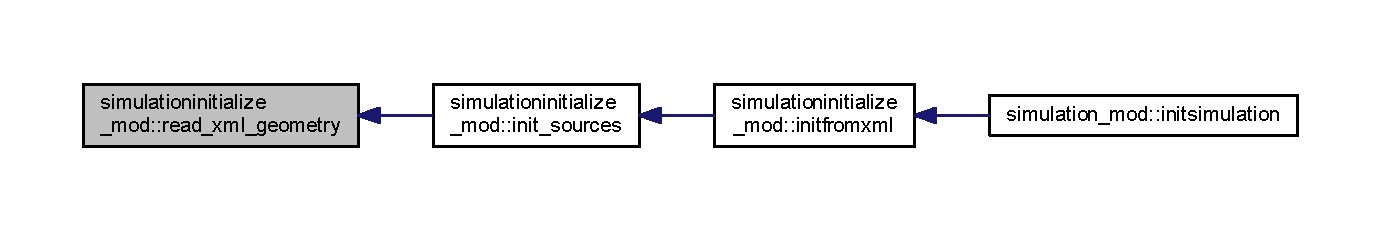
\includegraphics[width=350pt]{namespacesimulationinitialize__mod_ab65ac868a57f2cc124ec29f87a239424_icgraph}
\end{center}
\end{figure}
\mbox{\Hypertarget{namespacesimulationinitialize__mod_a09174fb4527277943700a5509de326dd}\label{namespacesimulationinitialize__mod_a09174fb4527277943700a5509de326dd}} 
\index{simulationinitialize\+\_\+mod@{simulationinitialize\+\_\+mod}!setoutputfields@{setoutputfields}}
\index{setoutputfields@{setoutputfields}!simulationinitialize\+\_\+mod@{simulationinitialize\+\_\+mod}}
\subsubsection{\texorpdfstring{setoutputfields()}{setoutputfields()}}
{\footnotesize\ttfamily subroutine simulationinitialize\+\_\+mod\+::setoutputfields (\begin{DoxyParamCaption}\item[{type(node), intent(in), pointer}]{exe\+Node }\end{DoxyParamCaption})\hspace{0.3cm}{\ttfamily [private]}}



Sets the global variables responsible for controling field outputs. reads options from a xml file and adds a variable field to the print poll accordingly. 

\begin{DoxyAuthor}{Author}
Ricardo Birjukovs Canelas -\/ M\+A\+R\+E\+T\+EC 
\end{DoxyAuthor}

\begin{DoxyParams}[1]{Parameters}
\mbox{\tt in}  & {\em exe\+Node} & \\
\hline
\end{DoxyParams}


Definition at line 158 of file simulation\+Initialize.\+f90.


\begin{DoxyCode}
158     \textcolor{keywordtype}{type}(Node), \textcolor{keywordtype}{intent(in)}, \textcolor{keywordtype}{pointer} :: exeNode
159     \textcolor{keywordtype}{type}(Node), \textcolor{keywordtype}{pointer} :: fileNode
160     \textcolor{keywordtype}{type}(Node), \textcolor{keywordtype}{pointer} :: fieldNode
161     \textcolor{keywordtype}{type}(Node), \textcolor{keywordtype}{pointer} :: outputFieldsFile
162     \textcolor{keywordtype}{type}(NodeList), \textcolor{keywordtype}{pointer} :: outputFieldsList
163     \textcolor{keywordtype}{type}(string) :: outext
164     \textcolor{keywordtype}{type}(string) :: tag, att\_name
165     \textcolor{keywordtype}{type}(string) :: outputFieldsFilename
166     \textcolor{keywordtype}{type}(string) :: fieldName, fieldOption
167     \textcolor{keywordtype}{type}(string), \textcolor{keywordtype}{dimension(:)}, \textcolor{keywordtype}{allocatable} :: fieldNameArray
168     \textcolor{keywordtype}{logical}, \textcolor{keywordtype}{dimension(:)}, \textcolor{keywordtype}{allocatable} :: toOutput
169     \textcolor{keywordtype}{integer} :: i
170     
171     tag=\textcolor{stringliteral}{"outputFields"} 
172     \textcolor{keyword}{call }xmlreader%gotoNode(exenode, filenode, tag, mandatory =.false.)
173     \textcolor{keywordflow}{if} (\textcolor{keyword}{associated}(filenode)) \textcolor{keywordflow}{then}
174         tag = \textcolor{stringliteral}{"file"}
175         \textcolor{keyword}{call }xmlreader%gotoNode(filenode, filenode, tag)
176         att\_name=\textcolor{stringliteral}{"name"}
177         \textcolor{keyword}{call }xmlreader%getLeafAttribute(filenode, att\_name, outputfieldsfilename)
178         \textcolor{comment}{!reading the file and building print/noprint array}
179         \textcolor{keyword}{call }xmlreader%getFile(outputfieldsfile, outputfieldsfilename)
180         tag = \textcolor{stringliteral}{"output"}
181         \textcolor{keyword}{call }xmlreader%gotoNode(outputfieldsfile ,outputfieldsfile, tag)
182         outputfieldslist => getelementsbytagname(outputfieldsfile, \textcolor{stringliteral}{"field"})
183         \textcolor{keyword}{allocate}(fieldnamearray(getlength(outputfieldslist)))
184         \textcolor{keyword}{allocate}(tooutput(getlength(outputfieldslist)))
185         tooutput = .false.
186         \textcolor{keywordflow}{do} i = 0, getlength(outputfieldslist) - 1
187             fieldnode => item(outputfieldslist, i)
188             att\_name=\textcolor{stringliteral}{"name"}
189             \textcolor{keyword}{call }xmlreader%getLeafAttribute(fieldnode, att\_name, fieldname)
190             att\_name=\textcolor{stringliteral}{"output"}
191             \textcolor{keyword}{call }xmlreader%getLeafAttribute(fieldnode, att\_name, fieldoption)
192             fieldnamearray(i+1) = fieldname
193             \textcolor{keywordflow}{if} (fieldoption == \textcolor{stringliteral}{'yes'}) tooutput(i+1) = .true.
194 \textcolor{keywordflow}{        end do}
195     \textcolor{keywordflow}{else}
196         outext=\textcolor{stringliteral}{'-->No output fields user override file, assuming basic settings for field output'}
197         \textcolor{keyword}{call }log%put(outext,.false.)
198 \textcolor{keywordflow}{    endif}
199     \textcolor{comment}{!calling the globals method to set the output variable field list}
200     \textcolor{keywordflow}{if} (.not.\textcolor{keyword}{allocated}(fieldnamearray)) \textcolor{keyword}{allocate}(fieldnamearray(0))
201     \textcolor{keyword}{call }globals%Output%setOutputFields(fieldnamearray, tooutput)
202 
\end{DoxyCode}
Here is the caller graph for this function\+:\nopagebreak
\begin{figure}[H]
\begin{center}
\leavevmode
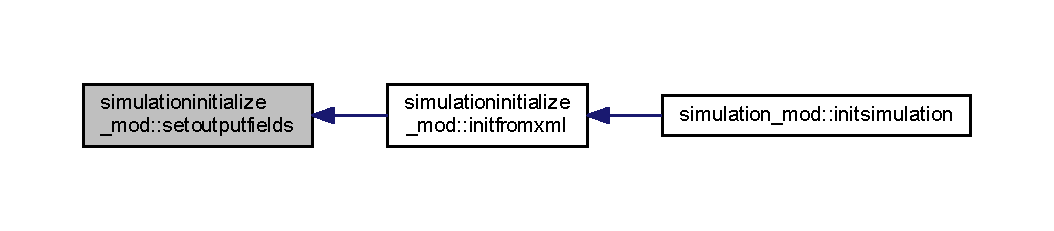
\includegraphics[width=350pt]{namespacesimulationinitialize__mod_a09174fb4527277943700a5509de326dd_icgraph}
\end{center}
\end{figure}

\hypertarget{namespacesimulationinputstreamer__mod}{}\section{simulationinputstreamer\+\_\+mod Module Reference}
\label{namespacesimulationinputstreamer__mod}\index{simulationinputstreamer\+\_\+mod@{simulationinputstreamer\+\_\+mod}}


Defines an input file reader class with an object exposable to the Simulation This class is in charge of selectig the correct reader for the selected input file format and controling the respective reader.  


\subsection*{Data Types}
\begin{DoxyCompactItemize}
\item 
type \mbox{\hyperlink{structsimulationinputstreamer__mod_1_1input__streamer__class}{input\+\_\+streamer\+\_\+class}}
\begin{DoxyCompactList}\small\item\em Input Streamer class. \end{DoxyCompactList}\item 
type \mbox{\hyperlink{structsimulationinputstreamer__mod_1_1inputfilemodel__class}{inputfilemodel\+\_\+class}}
\end{DoxyCompactItemize}
\subsection*{Functions/\+Subroutines}
\begin{DoxyCompactItemize}
\item 
subroutine \mbox{\hyperlink{namespacesimulationinputstreamer__mod_a3d4540f8e04cc0215895cad65c5be952}{loaddatafromstack}} (self, b\+Box, blocks)
\begin{DoxyCompactList}\small\item\em loads data from files and populates the backgrounds accordingly \end{DoxyCompactList}\item 
type(\mbox{\hyperlink{structbackground__mod_1_1background__class}{background\+\_\+class}}) function \mbox{\hyperlink{namespacesimulationinputstreamer__mod_a532b4022fdb6db20d41ca8082d4e7423}{getfullfile}} (self, file\+Name)
\begin{DoxyCompactList}\small\item\em instantiates and returns a background object with the data from a NC file \end{DoxyCompactList}\item 
subroutine \mbox{\hyperlink{namespacesimulationinputstreamer__mod_a0e5a1e43fe53f179325858d486a284e5}{initinputstreamer}} (self)
\begin{DoxyCompactList}\small\item\em Initializes the input writer object, imports metadata on input files. \end{DoxyCompactList}\item 
subroutine \mbox{\hyperlink{namespacesimulationinputstreamer__mod_a9465e29f527366e5f6d9a1195de6ddee}{resetreadstatus}} (self)
\begin{DoxyCompactList}\small\item\em resets input files read status \end{DoxyCompactList}\item 
subroutine \mbox{\hyperlink{namespacesimulationinputstreamer__mod_a1b906bc5ba1fac8d846b30237216aca4}{printinputstreamer}} (self)
\begin{DoxyCompactList}\small\item\em Prints the input writer object and metadata on input files. \end{DoxyCompactList}\end{DoxyCompactItemize}


\subsection{Detailed Description}
Defines an input file reader class with an object exposable to the Simulation This class is in charge of selectig the correct reader for the selected input file format and controling the respective reader. 

\begin{DoxyAuthor}{Author}
Ricardo Birjukovs Canelas 
\end{DoxyAuthor}


\subsection{Function/\+Subroutine Documentation}
\mbox{\Hypertarget{namespacesimulationinputstreamer__mod_a532b4022fdb6db20d41ca8082d4e7423}\label{namespacesimulationinputstreamer__mod_a532b4022fdb6db20d41ca8082d4e7423}} 
\index{simulationinputstreamer\+\_\+mod@{simulationinputstreamer\+\_\+mod}!getfullfile@{getfullfile}}
\index{getfullfile@{getfullfile}!simulationinputstreamer\+\_\+mod@{simulationinputstreamer\+\_\+mod}}
\subsubsection{\texorpdfstring{getfullfile()}{getfullfile()}}
{\footnotesize\ttfamily type(\mbox{\hyperlink{structbackground__mod_1_1background__class}{background\+\_\+class}}) function simulationinputstreamer\+\_\+mod\+::getfullfile (\begin{DoxyParamCaption}\item[{class(\mbox{\hyperlink{structsimulationinputstreamer__mod_1_1input__streamer__class}{input\+\_\+streamer\+\_\+class}}), intent(in)}]{self,  }\item[{type(string), intent(in)}]{file\+Name }\end{DoxyParamCaption})\hspace{0.3cm}{\ttfamily [private]}}



instantiates and returns a background object with the data from a NC file 

\begin{DoxyAuthor}{Author}
Ricardo Birjukovs Canelas -\/ M\+A\+R\+E\+T\+EC 
\end{DoxyAuthor}

\begin{DoxyParams}[1]{Parameters}
\mbox{\tt in}  & {\em self,nfile} & \\
\hline
\end{DoxyParams}


Definition at line 128 of file simulation\+Input\+Streamer.\+f90.


\begin{DoxyCode}
128     \textcolor{keywordtype}{class}(input\_streamer\_class), \textcolor{keywordtype}{intent(in)} :: self
129     \textcolor{keywordtype}{type}(string), \textcolor{keywordtype}{intent(in)} :: fileName
130     \textcolor{keywordtype}{type}(ncfile\_class) :: ncFile
131     \textcolor{keywordtype}{type}(scalar1d\_field\_class), \textcolor{keywordtype}{allocatable}, \textcolor{keywordtype}{dimension(:)} :: backgrounDims
132     \textcolor{keywordtype}{type}(generic\_field\_class), \textcolor{keywordtype}{allocatable}, \textcolor{keywordtype}{dimension(:)} :: gfield
133     \textcolor{keywordtype}{type}(string) :: name, units
134     \textcolor{keywordtype}{type}(box) :: extents
135     \textcolor{keywordtype}{type}(vector) :: pt
136     \textcolor{keywordtype}{real(prec)}, \textcolor{keywordtype}{dimension(3,2)} :: dimExtents
137     \textcolor{keywordtype}{integer} :: i
138     \textcolor{keywordtype}{type}(string) :: outext
139 
140     \textcolor{keyword}{allocate}(gfield(5))
141 
142     outext = \textcolor{stringliteral}{'->Reading '}//filename
143     \textcolor{keyword}{call }log%put(outext,.false.)
144 
145     \textcolor{keyword}{call }ncfile%initialize(filename)
146     \textcolor{keyword}{call }ncfile%getVarDimensions(globals%Var%u, backgroundims)
147     \textcolor{keyword}{call }ncfile%getVar(globals%Var%u, gfield(1))
148     \textcolor{keyword}{call }ncfile%getVar(globals%Var%v, gfield(2))
149     \textcolor{keyword}{call }ncfile%getVar(globals%Var%w, gfield(3))
150     \textcolor{comment}{!reading a field to use later as land mask}
151     units = \textcolor{stringliteral}{'-'}
152     \textcolor{keyword}{call }ncfile%getVar(globals%Var%u, gfield(4), .true., globals%Var%landMask, units)
153     \textcolor{keyword}{call }ncfile%getVar(globals%Var%u, gfield(5), .true., globals%Var%landIntMask, units)
154     \textcolor{comment}{!finalizing reader}
155     \textcolor{keyword}{call }ncfile%finalize()
156 
157     dimextents = 0.0
158     \textcolor{keywordflow}{do} i = 1, \textcolor{keyword}{size}(backgroundims)
159         \textcolor{keywordflow}{if} (backgroundims(i)%name == globals%Var%lon) \textcolor{keywordflow}{then}
160             dimextents(1,1) = backgroundims(i)%getFieldMinBound()
161             dimextents(1,2) = backgroundims(i)%getFieldMaxBound()
162         \textcolor{keywordflow}{else} \textcolor{keywordflow}{if} (backgroundims(i)%name == globals%Var%lat) \textcolor{keywordflow}{then}
163             dimextents(2,1) = backgroundims(i)%getFieldMinBound()
164             dimextents(2,2) = backgroundims(i)%getFieldMaxBound()
165         \textcolor{keywordflow}{else} \textcolor{keywordflow}{if} (backgroundims(i)%name == globals%Var%level) \textcolor{keywordflow}{then}
166             dimextents(3,1) = backgroundims(i)%getFieldMinBound()
167             dimextents(3,2) = backgroundims(i)%getFieldMaxBound()
168 \textcolor{keywordflow}{        end if}
169 \textcolor{keywordflow}{    end do}
170     extents%pt = dimextents(1,1)*ex + dimextents(2,1)*ey + dimextents(3,1)*ez
171     pt = dimextents(1,2)*ex + dimextents(2,2)*ey + dimextents(3,2)*ez
172     extents%size = pt - extents%pt
173 
174     name = filename%basename(strip\_last\_extension=.true.)
175     getfullfile = background(1, name, extents, backgroundims)
176     \textcolor{keywordflow}{do} i = 1, \textcolor{keyword}{size}(gfield)
177         \textcolor{keyword}{call }getfullfile%add(gfield(i))
178         \textcolor{comment}{!call gfield(i)%print()}
179         \textcolor{keyword}{call }gfield(i)%finalize()
180 \textcolor{keywordflow}{    end do}
181     
182     \textcolor{keyword}{call }getfullfile%makeLandMask()
183     
184     \textcolor{comment}{!call getFullFile%print()}
185 
\end{DoxyCode}
\mbox{\Hypertarget{namespacesimulationinputstreamer__mod_a0e5a1e43fe53f179325858d486a284e5}\label{namespacesimulationinputstreamer__mod_a0e5a1e43fe53f179325858d486a284e5}} 
\index{simulationinputstreamer\+\_\+mod@{simulationinputstreamer\+\_\+mod}!initinputstreamer@{initinputstreamer}}
\index{initinputstreamer@{initinputstreamer}!simulationinputstreamer\+\_\+mod@{simulationinputstreamer\+\_\+mod}}
\subsubsection{\texorpdfstring{initinputstreamer()}{initinputstreamer()}}
{\footnotesize\ttfamily subroutine simulationinputstreamer\+\_\+mod\+::initinputstreamer (\begin{DoxyParamCaption}\item[{class(\mbox{\hyperlink{structsimulationinputstreamer__mod_1_1input__streamer__class}{input\+\_\+streamer\+\_\+class}}), intent(inout)}]{self }\end{DoxyParamCaption})\hspace{0.3cm}{\ttfamily [private]}}



Initializes the input writer object, imports metadata on input files. 

\begin{DoxyAuthor}{Author}
Ricardo Birjukovs Canelas -\/ M\+A\+R\+E\+T\+EC 
\end{DoxyAuthor}


Definition at line 194 of file simulation\+Input\+Streamer.\+f90.


\begin{DoxyCode}
194     \textcolor{keywordtype}{class}(input\_streamer\_class), \textcolor{keywordtype}{intent(inout)} :: self
195     \textcolor{keywordtype}{type}(Node), \textcolor{keywordtype}{pointer} :: xmlInputs
196     \textcolor{keywordtype}{type}(Node), \textcolor{keywordtype}{pointer} :: fileNode
197     \textcolor{keywordtype}{type}(NodeList), \textcolor{keywordtype}{pointer} :: fileList
198     \textcolor{keywordtype}{type}(string) :: tag, att\_name, att\_val
199     \textcolor{keywordtype}{type}(string), \textcolor{keywordtype}{allocatable}, \textcolor{keywordtype}{dimension(:)} :: fileNames
200     \textcolor{keywordtype}{integer} :: i
201 
202     self%bufferSize = globals%Parameters%BufferSize
203     self%lastReadTime = -1.0
204 
205     \textcolor{keyword}{call }xmlreader%getFile(xmlinputs,globals%Names%inputsXmlFilename, mandatory = .false.)
206     \textcolor{keywordflow}{if} (\textcolor{keyword}{associated}(xmlinputs)) \textcolor{keywordflow}{then}
207         self%useInputFiles = .true.
208         \textcolor{comment}{!Go to the file\_collection node}
209         tag = \textcolor{stringliteral}{"file\_collection"}
210         \textcolor{keyword}{call }xmlreader%gotoNode(xmlinputs,xmlinputs,tag)
211         tag = \textcolor{stringliteral}{"currents"}
212         \textcolor{keyword}{call }xmlreader%gotoNode(xmlinputs,xmlinputs,tag)
213         filelist => getelementsbytagname(xmlinputs, \textcolor{stringliteral}{"file"})       \textcolor{comment}{!searching for tags with the 'namingfile'
       name}
214         \textcolor{keyword}{allocate}(filenames(getlength(filelist)))
215         \textcolor{keyword}{allocate}(self%currentsInputFile(getlength(filelist)))
216         \textcolor{keywordflow}{do} i = 0, getlength(filelist) - 1
217             filenode => item(filelist, i)
218             tag=\textcolor{stringliteral}{"name"}
219             att\_name=\textcolor{stringliteral}{"value"}
220             \textcolor{keyword}{call }xmlreader%getNodeAttribute(filenode, tag, att\_name, filenames(i+1))
221             self%currentsInputFile(i+1)%name = filenames(i+1)
222             tag=\textcolor{stringliteral}{"startTime"}
223             att\_name=\textcolor{stringliteral}{"value"}
224             \textcolor{keyword}{call }xmlreader%getNodeAttribute(filenode, tag, att\_name, att\_val)
225             self%currentsInputFile(i+1)%startTime = att\_val%to\_number(kind=1.\_r4p)
226             tag=\textcolor{stringliteral}{"endTime"}
227             att\_name=\textcolor{stringliteral}{"value"}
228             \textcolor{keyword}{call }xmlreader%getNodeAttribute(filenode, tag, att\_name, att\_val)
229             self%currentsInputFile(i+1)%endTime = att\_val%to\_number(kind=1.\_r4p)
230             self%currentsInputFile(i+1)%used = .false.
231 \textcolor{keywordflow}{        end do}
232         \textcolor{keyword}{call }globals%setInputFileNames(filenames)
233     \textcolor{keywordflow}{else}
234         self%useInputFiles = .false.
235 \textcolor{keywordflow}{    end if}
\end{DoxyCode}
\mbox{\Hypertarget{namespacesimulationinputstreamer__mod_a3d4540f8e04cc0215895cad65c5be952}\label{namespacesimulationinputstreamer__mod_a3d4540f8e04cc0215895cad65c5be952}} 
\index{simulationinputstreamer\+\_\+mod@{simulationinputstreamer\+\_\+mod}!loaddatafromstack@{loaddatafromstack}}
\index{loaddatafromstack@{loaddatafromstack}!simulationinputstreamer\+\_\+mod@{simulationinputstreamer\+\_\+mod}}
\subsubsection{\texorpdfstring{loaddatafromstack()}{loaddatafromstack()}}
{\footnotesize\ttfamily subroutine simulationinputstreamer\+\_\+mod\+::loaddatafromstack (\begin{DoxyParamCaption}\item[{class(\mbox{\hyperlink{structsimulationinputstreamer__mod_1_1input__streamer__class}{input\+\_\+streamer\+\_\+class}}), intent(inout)}]{self,  }\item[{type(\mbox{\hyperlink{structboundingbox__mod_1_1boundingbox__class}{boundingbox\+\_\+class}}), intent(in)}]{b\+Box,  }\item[{type(\mbox{\hyperlink{structblocks__mod_1_1block__class}{block\+\_\+class}}), dimension(\+:), intent(inout)}]{blocks }\end{DoxyParamCaption})\hspace{0.3cm}{\ttfamily [private]}}



loads data from files and populates the backgrounds accordingly 

\begin{DoxyAuthor}{Author}
Ricardo Birjukovs Canelas -\/ M\+A\+R\+E\+T\+EC 
\end{DoxyAuthor}

\begin{DoxyParams}[1]{Parameters}
\mbox{\tt in}  & {\em self,bbox,blocks} & \\
\hline
\mbox{\tt in}  & {\em bbox} & Case bounding box\\
\hline
\mbox{\tt in,out}  & {\em blocks} & Case Blocks \\
\hline
\end{DoxyParams}


Definition at line 71 of file simulation\+Input\+Streamer.\+f90.


\begin{DoxyCode}
71     \textcolor{keywordtype}{class}(input\_streamer\_class), \textcolor{keywordtype}{intent(inout)} :: self
72     \textcolor{keywordtype}{type}(boundingbox\_class), \textcolor{keywordtype}{intent(in)} :: bBox
73     \textcolor{keywordtype}{type}(block\_class), \textcolor{keywordtype}{dimension(:)}, \textcolor{keywordtype}{intent(inout)} :: blocks
74     \textcolor{keywordtype}{type}(background\_class) :: tempBkgd
75     \textcolor{keywordtype}{integer} :: i, j
76     \textcolor{keywordtype}{integer} :: fNumber
77     \textcolor{keywordtype}{real(prec)} :: tempTime(2)
78     \textcolor{keywordtype}{logical} :: needToRead, appended
79 
80     needtoread = .false.
81     \textcolor{keywordflow}{if} (self%useInputFiles) \textcolor{keywordflow}{then}
82         \textcolor{comment}{!check if we need to import data (current time and buffer size)}
83         \textcolor{keywordflow}{if} (self%lastReadTime <= globals%SimTime%CurrTime + self%BufferSize/4.0) needtoread = .true.
84         \textcolor{keywordflow}{if} (self%lastReadTime >= globals%SimTime%TimeMax) needtoread = .false.
85         \textcolor{keywordflow}{if} (needtoread) \textcolor{keywordflow}{then}
86             \textcolor{keyword}{call }self%resetReadStatus()
87             \textcolor{comment}{!check what files on the stack are to read to backgrounds}
88             \textcolor{keywordflow}{do} i=1, \textcolor{keyword}{size}(self%currentsInputFile)
89                 \textcolor{keywordflow}{if} (self%currentsInputFile(i)%endTime >= globals%SimTime%CurrTime) \textcolor{keywordflow}{then}
90                     \textcolor{keywordflow}{if} (self%currentsInputFile(i)%startTime <= globals%SimTime%CurrTime + self%BufferSize) \textcolor{keywordflow}{
      then}
91                         \textcolor{keywordflow}{if} (.not.self%currentsInputFile(i)%used) self%currentsInputFile(i)%toRead = .true.
92 \textcolor{keywordflow}{                    end if}
93 \textcolor{keywordflow}{                end if}
94 \textcolor{keywordflow}{            end do}
95             \textcolor{comment}{!read selected files}
96             \textcolor{keywordflow}{do} i=1, \textcolor{keyword}{size}(self%currentsInputFile)
97                 \textcolor{keywordflow}{if} (self%currentsInputFile(i)%toRead) \textcolor{keywordflow}{then}
98                     \textcolor{comment}{!import data to temporary background}
99                     tempbkgd = self%getFullFile(self%currentsInputFile(i)%name)
100                     self%currentsInputFile(i)%used = .true.
101                     \textcolor{keywordflow}{do} j=1, \textcolor{keyword}{size}(blocks)
102                         \textcolor{keywordflow}{if} (.not.\textcolor{keyword}{allocated}(blocks(j)%Background)) \textcolor{keyword}{allocate}(blocks(j)%Background(1))
103                         \textcolor{comment}{!slice data by block and either join to existing background or add a new one}
104                         \textcolor{keywordflow}{if} (blocks(j)%Background(1)%initialized) \textcolor{keyword}{call }blocks(j)%Background(1)%append(
      tempbkgd%getHyperSlab(blocks(j)%extents), appended)
105                         \textcolor{keywordflow}{if} (.not.blocks(j)%Background(1)%initialized) blocks(j)%Background(1) = tempbkgd
      %getHyperSlab(blocks(j)%extents)
106 
107                         \textcolor{comment}{!save last time already loaded}
108                         temptime = blocks(j)%Background(1)%getDimExtents(globals%Var%time)
109                         self%lastReadTime = temptime(2)
110 
111 \textcolor{keywordflow}{                    end do}
112                     \textcolor{comment}{!clean out the temporary background data (this structure, even tough it is a local
       variable, has pointers inside)}
113                     \textcolor{keyword}{call }tempbkgd%finalize()
114 \textcolor{keywordflow}{                end if}
115 \textcolor{keywordflow}{            end do}
116 \textcolor{keywordflow}{        end if}
117 \textcolor{keywordflow}{    end if}
118 
\end{DoxyCode}
\mbox{\Hypertarget{namespacesimulationinputstreamer__mod_a1b906bc5ba1fac8d846b30237216aca4}\label{namespacesimulationinputstreamer__mod_a1b906bc5ba1fac8d846b30237216aca4}} 
\index{simulationinputstreamer\+\_\+mod@{simulationinputstreamer\+\_\+mod}!printinputstreamer@{printinputstreamer}}
\index{printinputstreamer@{printinputstreamer}!simulationinputstreamer\+\_\+mod@{simulationinputstreamer\+\_\+mod}}
\subsubsection{\texorpdfstring{printinputstreamer()}{printinputstreamer()}}
{\footnotesize\ttfamily subroutine simulationinputstreamer\+\_\+mod\+::printinputstreamer (\begin{DoxyParamCaption}\item[{class(\mbox{\hyperlink{structsimulationinputstreamer__mod_1_1input__streamer__class}{input\+\_\+streamer\+\_\+class}}), intent(in)}]{self }\end{DoxyParamCaption})\hspace{0.3cm}{\ttfamily [private]}}



Prints the input writer object and metadata on input files. 

\begin{DoxyAuthor}{Author}
Ricardo Birjukovs Canelas -\/ M\+A\+R\+E\+T\+EC 
\end{DoxyAuthor}


Definition at line 257 of file simulation\+Input\+Streamer.\+f90.


\begin{DoxyCode}
257     \textcolor{keywordtype}{class}(input\_streamer\_class), \textcolor{keywordtype}{intent(in)} :: self
258     \textcolor{keywordtype}{type}(string) :: outext, temp\_str
259     \textcolor{keywordtype}{integer} :: i
260     outext = \textcolor{stringliteral}{'-->Input streamer stack:'}//new\_line(\textcolor{stringliteral}{'a'})
261     outext = outext//\textcolor{stringliteral}{'--->Currents data '}
262     \textcolor{keywordflow}{do} i=1, \textcolor{keyword}{size}(self%currentsInputFile)
263         outext = outext//new\_line(\textcolor{stringliteral}{'a'})
264         outext = outext//\textcolor{stringliteral}{'---->File '}//self%currentsInputFile(i)%name\textcolor{comment}{!//new\_line('a')}
265         \textcolor{comment}{!temp\_str=self%currentsInputFile(i)%startTime}
266         \textcolor{comment}{!outext = outext//'      Starting time is '//temp\_str//' s'//new\_line('a')}
267         \textcolor{comment}{!temp\_str=self%currentsInputFile(i)%endTime}
268         \textcolor{comment}{!outext = outext//'      Ending time is   '//temp\_str//' s'}
269 \textcolor{keywordflow}{    end do}
270     \textcolor{keywordflow}{if} (.not.self%useInputFiles) outext = \textcolor{stringliteral}{'-->Input streamer stack is empty, no input data'}
271     \textcolor{keyword}{call }log%put(outext,.false.)
\end{DoxyCode}
\mbox{\Hypertarget{namespacesimulationinputstreamer__mod_a9465e29f527366e5f6d9a1195de6ddee}\label{namespacesimulationinputstreamer__mod_a9465e29f527366e5f6d9a1195de6ddee}} 
\index{simulationinputstreamer\+\_\+mod@{simulationinputstreamer\+\_\+mod}!resetreadstatus@{resetreadstatus}}
\index{resetreadstatus@{resetreadstatus}!simulationinputstreamer\+\_\+mod@{simulationinputstreamer\+\_\+mod}}
\subsubsection{\texorpdfstring{resetreadstatus()}{resetreadstatus()}}
{\footnotesize\ttfamily subroutine simulationinputstreamer\+\_\+mod\+::resetreadstatus (\begin{DoxyParamCaption}\item[{class(\mbox{\hyperlink{structsimulationinputstreamer__mod_1_1input__streamer__class}{input\+\_\+streamer\+\_\+class}}), intent(inout)}]{self }\end{DoxyParamCaption})\hspace{0.3cm}{\ttfamily [private]}}



resets input files read status 

\begin{DoxyAuthor}{Author}
Ricardo Birjukovs Canelas -\/ M\+A\+R\+E\+T\+EC 
\end{DoxyAuthor}


Definition at line 244 of file simulation\+Input\+Streamer.\+f90.


\begin{DoxyCode}
244     \textcolor{keywordtype}{class}(input\_streamer\_class), \textcolor{keywordtype}{intent(inout)} :: self
245     \textcolor{keywordtype}{integer} :: i
246     \textcolor{keywordflow}{do} i=1, \textcolor{keyword}{size}(self%currentsInputFile)
247         self%currentsInputFile(i)%toRead = .false.
248 \textcolor{keywordflow}{    end do}
\end{DoxyCode}

\hypertarget{namespacesimulationlogger__mod}{}\section{simulationlogger\+\_\+mod Module Reference}
\label{namespacesimulationlogger__mod}\index{simulationlogger\+\_\+mod@{simulationlogger\+\_\+mod}}


Module to hold all the simulation logger related definitions and methods.  


\subsection*{Data Types}
\begin{DoxyCompactItemize}
\item 
type \mbox{\hyperlink{structsimulationlogger__mod_1_1logger__class}{logger\+\_\+class}}
\end{DoxyCompactItemize}
\subsection*{Functions/\+Subroutines}
\begin{DoxyCompactItemize}
\item 
subroutine \mbox{\hyperlink{namespacesimulationlogger__mod_aeb57075501eed504789bb5858b4e6b59}{initlog}} (self, outpath)
\begin{DoxyCompactList}\small\item\em Log file initizalization routine. \end{DoxyCompactList}\item 
subroutine \mbox{\hyperlink{namespacesimulationlogger__mod_a9cad2fd4ad67dc229286f94b0444cb86}{closelog}} (self)
\begin{DoxyCompactList}\small\item\em Log file closure routine. \end{DoxyCompactList}\item 
subroutine \mbox{\hyperlink{namespacesimulationlogger__mod_a3bf437b875b454ef326a3bc660542539}{put\+\_\+inlog}} (self, tologstr, timeoption)
\begin{DoxyCompactList}\small\item\em Log serialization routine. \end{DoxyCompactList}\item 
subroutine, public \mbox{\hyperlink{namespacesimulationlogger__mod_abff1db7e1655cb59097146d78e650672}{gettimestamp}} (timestamp)
\begin{DoxyCompactList}\small\item\em Public timestamp builder. \end{DoxyCompactList}\end{DoxyCompactItemize}
\subsection*{Variables}
\begin{DoxyCompactItemize}
\item 
type(\mbox{\hyperlink{structsimulationlogger__mod_1_1logger__class}{logger\+\_\+class}}), public \mbox{\hyperlink{namespacesimulationlogger__mod_a0d667ffec2a1129f89f4bd8fe6dc8a43}{log}}
\end{DoxyCompactItemize}


\subsection{Detailed Description}
Module to hold all the simulation logger related definitions and methods. 

\begin{DoxyAuthor}{Author}
Ricardo Birjukovs Canelas 
\end{DoxyAuthor}


\subsection{Function/\+Subroutine Documentation}
\mbox{\Hypertarget{namespacesimulationlogger__mod_a9cad2fd4ad67dc229286f94b0444cb86}\label{namespacesimulationlogger__mod_a9cad2fd4ad67dc229286f94b0444cb86}} 
\index{simulationlogger\+\_\+mod@{simulationlogger\+\_\+mod}!closelog@{closelog}}
\index{closelog@{closelog}!simulationlogger\+\_\+mod@{simulationlogger\+\_\+mod}}
\subsubsection{\texorpdfstring{closelog()}{closelog()}}
{\footnotesize\ttfamily subroutine simulationlogger\+\_\+mod\+::closelog (\begin{DoxyParamCaption}\item[{class(\mbox{\hyperlink{structsimulationlogger__mod_1_1logger__class}{logger\+\_\+class}}), intent(inout)}]{self }\end{DoxyParamCaption})\hspace{0.3cm}{\ttfamily [private]}}



Log file closure routine. 

\begin{DoxyAuthor}{Author}
Ricardo Birjukovs Canelas -\/ M\+A\+R\+E\+T\+EC 
\end{DoxyAuthor}


Definition at line 74 of file simulation\+Logger.\+f90.


\begin{DoxyCode}
74     \textcolor{keywordtype}{implicit none}
75     \textcolor{keywordtype}{class}(logger\_class), \textcolor{keywordtype}{intent(inout)} :: self
76     \textcolor{keyword}{close}(self%log\_unit)
\end{DoxyCode}
\mbox{\Hypertarget{namespacesimulationlogger__mod_abff1db7e1655cb59097146d78e650672}\label{namespacesimulationlogger__mod_abff1db7e1655cb59097146d78e650672}} 
\index{simulationlogger\+\_\+mod@{simulationlogger\+\_\+mod}!gettimestamp@{gettimestamp}}
\index{gettimestamp@{gettimestamp}!simulationlogger\+\_\+mod@{simulationlogger\+\_\+mod}}
\subsubsection{\texorpdfstring{gettimestamp()}{gettimestamp()}}
{\footnotesize\ttfamily subroutine, public simulationlogger\+\_\+mod\+::gettimestamp (\begin{DoxyParamCaption}\item[{type(string), intent(out)}]{timestamp }\end{DoxyParamCaption})}



Public timestamp builder. 

\begin{DoxyAuthor}{Author}
Ricardo Birjukovs Canelas -\/ M\+A\+R\+E\+T\+EC 
\end{DoxyAuthor}

\begin{DoxyParams}[1]{Parameters}
\mbox{\tt in}  & {\em timestamp} & \\
\hline
\end{DoxyParams}


Definition at line 111 of file simulation\+Logger.\+f90.


\begin{DoxyCode}
111     \textcolor{keywordtype}{type}(string), \textcolor{keywordtype}{intent(out)} :: timestamp
112     \textcolor{keywordtype}{type}(datetime) :: date   
113     date = date%now()
114     timestamp = date%isoformat(\textcolor{stringliteral}{' '})
115     timestamp = timestamp%basename(strip\_last\_extension=.true.) \textcolor{comment}{!getting rid of miliseconds}
\end{DoxyCode}
Here is the caller graph for this function\+:\nopagebreak
\begin{figure}[H]
\begin{center}
\leavevmode
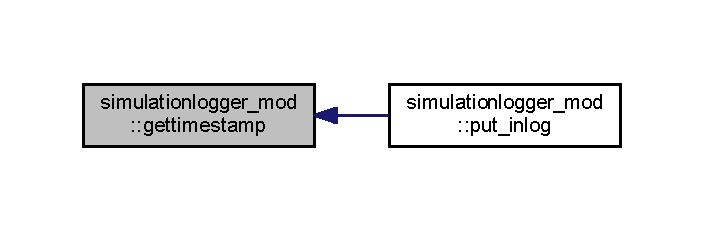
\includegraphics[width=338pt]{namespacesimulationlogger__mod_abff1db7e1655cb59097146d78e650672_icgraph}
\end{center}
\end{figure}
\mbox{\Hypertarget{namespacesimulationlogger__mod_aeb57075501eed504789bb5858b4e6b59}\label{namespacesimulationlogger__mod_aeb57075501eed504789bb5858b4e6b59}} 
\index{simulationlogger\+\_\+mod@{simulationlogger\+\_\+mod}!initlog@{initlog}}
\index{initlog@{initlog}!simulationlogger\+\_\+mod@{simulationlogger\+\_\+mod}}
\subsubsection{\texorpdfstring{initlog()}{initlog()}}
{\footnotesize\ttfamily subroutine simulationlogger\+\_\+mod\+::initlog (\begin{DoxyParamCaption}\item[{class(\mbox{\hyperlink{structsimulationlogger__mod_1_1logger__class}{logger\+\_\+class}}), intent(inout)}]{self,  }\item[{type(string), intent(in)}]{outpath }\end{DoxyParamCaption})\hspace{0.3cm}{\ttfamily [private]}}



Log file initizalization routine. 

\begin{DoxyAuthor}{Author}
Ricardo Birjukovs Canelas -\/ M\+A\+R\+E\+T\+EC 
\end{DoxyAuthor}

\begin{DoxyParams}[1]{Parameters}
\mbox{\tt in}  & {\em self,outpath} & \\
\hline
\mbox{\tt in}  & {\em outpath} & output path were to point the logger \\
\hline
\end{DoxyParams}


Definition at line 57 of file simulation\+Logger.\+f90.


\begin{DoxyCode}
57     \textcolor{keywordtype}{implicit none}
58     \textcolor{keywordtype}{class}(logger\_class), \textcolor{keywordtype}{intent(inout)} :: self
59     \textcolor{keywordtype}{type}(string), \textcolor{keywordtype}{intent(in)} :: outpath
60     \textcolor{keywordtype}{type}(string) :: logfile
61 
62     logfile = outpath//\textcolor{stringliteral}{'MOHIDLagrangianRun.out'}
63     self%log\_unit = 0
64     \textcolor{keyword}{open} (unit=self%log\_unit,file=logfile%chars(),action=\textcolor{stringliteral}{"write"},status=\textcolor{stringliteral}{"replace"})
65 
\end{DoxyCode}
\mbox{\Hypertarget{namespacesimulationlogger__mod_a3bf437b875b454ef326a3bc660542539}\label{namespacesimulationlogger__mod_a3bf437b875b454ef326a3bc660542539}} 
\index{simulationlogger\+\_\+mod@{simulationlogger\+\_\+mod}!put\+\_\+inlog@{put\+\_\+inlog}}
\index{put\+\_\+inlog@{put\+\_\+inlog}!simulationlogger\+\_\+mod@{simulationlogger\+\_\+mod}}
\subsubsection{\texorpdfstring{put\+\_\+inlog()}{put\_inlog()}}
{\footnotesize\ttfamily subroutine simulationlogger\+\_\+mod\+::put\+\_\+inlog (\begin{DoxyParamCaption}\item[{class(\mbox{\hyperlink{structsimulationlogger__mod_1_1logger__class}{logger\+\_\+class}}), intent(in)}]{self,  }\item[{type(string), intent(inout)}]{tologstr,  }\item[{logical, intent(in), optional}]{timeoption }\end{DoxyParamCaption})\hspace{0.3cm}{\ttfamily [private]}}



Log serialization routine. 

\begin{DoxyAuthor}{Author}
Ricardo Birjukovs Canelas -\/ M\+A\+R\+E\+T\+EC 
\end{DoxyAuthor}

\begin{DoxyParams}[1]{Parameters}
\mbox{\tt in}  & {\em self,tologstr,timeoption} & \\
\hline
\end{DoxyParams}


Definition at line 86 of file simulation\+Logger.\+f90.


\begin{DoxyCode}
86     \textcolor{keywordtype}{implicit none}
87     \textcolor{keywordtype}{class}(logger\_class), \textcolor{keywordtype}{intent(in)} :: self
88     \textcolor{keywordtype}{type}(string), \textcolor{keywordtype}{intent(inout)} :: tologstr
89     \textcolor{keywordtype}{logical}, \textcolor{keywordtype}{intent(in)}, \textcolor{keywordtype}{optional} :: timeoption
90     \textcolor{keywordtype}{type}(string) :: timestamp
91 
92     \textcolor{keyword}{call }gettimestamp(timestamp)
93     \textcolor{keywordflow}{if} (\textcolor{keyword}{present}(timeoption)) \textcolor{keywordflow}{then}
94         \textcolor{keywordflow}{if} (.not.timeoption) \textcolor{keywordflow}{then}
95             timestamp=\textcolor{stringliteral}{''}
96 \textcolor{keywordflow}{        endif}
97 \textcolor{keywordflow}{    endif}
98     tologstr=timestamp//\textcolor{stringliteral}{' '}//tologstr
99     \textcolor{keyword}{write}(self%log\_unit,\textcolor{stringliteral}{"(A)"}) tologstr%chars()
100     print\textcolor{stringliteral}{'(A)'}, tologstr%chars()
101 
\end{DoxyCode}
Here is the call graph for this function\+:\nopagebreak
\begin{figure}[H]
\begin{center}
\leavevmode
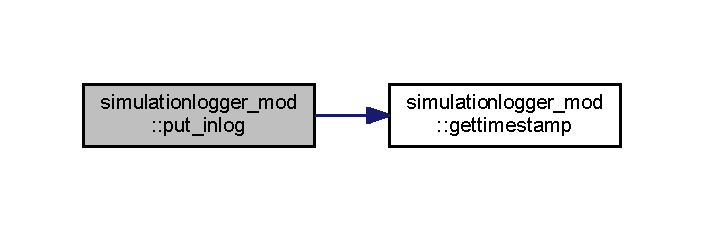
\includegraphics[width=338pt]{namespacesimulationlogger__mod_a3bf437b875b454ef326a3bc660542539_cgraph}
\end{center}
\end{figure}


\subsection{Variable Documentation}
\mbox{\Hypertarget{namespacesimulationlogger__mod_a0d667ffec2a1129f89f4bd8fe6dc8a43}\label{namespacesimulationlogger__mod_a0d667ffec2a1129f89f4bd8fe6dc8a43}} 
\index{simulationlogger\+\_\+mod@{simulationlogger\+\_\+mod}!log@{log}}
\index{log@{log}!simulationlogger\+\_\+mod@{simulationlogger\+\_\+mod}}
\subsubsection{\texorpdfstring{log}{log}}
{\footnotesize\ttfamily type(\mbox{\hyperlink{structsimulationlogger__mod_1_1logger__class}{logger\+\_\+class}}), public simulationlogger\+\_\+mod\+::log}



Definition at line 40 of file simulation\+Logger.\+f90.


\begin{DoxyCode}
40     \textcolor{keywordtype}{type}(logger\_class) :: Log
\end{DoxyCode}

\hypertarget{namespacesimulationmemory__mod}{}\section{simulationmemory\+\_\+mod Module Reference}
\label{namespacesimulationmemory__mod}\index{simulationmemory\+\_\+mod@{simulationmemory\+\_\+mod}}


Module to hold the simulation memory managment class and its methods.  


\subsection*{Data Types}
\begin{DoxyCompactItemize}
\item 
type \mbox{\hyperlink{structsimulationmemory__mod_1_1memory__t}{memory\+\_\+t}}
\end{DoxyCompactItemize}
\subsection*{Functions/\+Subroutines}
\begin{DoxyCompactItemize}
\item 
subroutine \mbox{\hyperlink{namespacesimulationmemory__mod_afaf06c4001ebc289c12a9358a99d224d}{initializememory}} (self)
\begin{DoxyCompactList}\small\item\em Memory logger initialization method. \end{DoxyCompactList}\item 
subroutine \mbox{\hyperlink{namespacesimulationmemory__mod_a3eb0ad61a559664ed4227ca4ad1746af}{getotal}} (self, size)
\begin{DoxyCompactList}\small\item\em Method to retreive the total size of the allocated memory. \end{DoxyCompactList}\item 
subroutine \mbox{\hyperlink{namespacesimulationmemory__mod_a936043befeeb2a3a79b31b519295b842}{setntrc}} (self, ntrc)
\begin{DoxyCompactList}\small\item\em Method to set the total expected number of Tracers. \end{DoxyCompactList}\item 
subroutine \mbox{\hyperlink{namespacesimulationmemory__mod_a48844ee646c6d29108f5bb1bdb9fd1bf}{setsizetrc}} (self, size\+Trc)
\begin{DoxyCompactList}\small\item\em Method to set the size of a typical Tracer. \end{DoxyCompactList}\item 
subroutine \mbox{\hyperlink{namespacesimulationmemory__mod_a2ade4b86d68e8daa4f22e1cdf7473e2c}{addblock}} (self, size)
\begin{DoxyCompactList}\small\item\em Method to add the size of a Block to the memory log. \end{DoxyCompactList}\item 
subroutine \mbox{\hyperlink{namespacesimulationmemory__mod_ae5682757ed7e3e005a1b54e5b44ed8a1}{addsource}} (self, size)
\begin{DoxyCompactList}\small\item\em Method to add the size of a Source to the memory log. \end{DoxyCompactList}\item 
subroutine \mbox{\hyperlink{namespacesimulationmemory__mod_a3209dc0fdd14fe4a6190e67607076f65}{setracer}} (self, size)
\begin{DoxyCompactList}\small\item\em Method to add the size of a Tracer to the memory log. \end{DoxyCompactList}\item 
subroutine \mbox{\hyperlink{namespacesimulationmemory__mod_a0812b4222f930cfb142586f47b2de0da}{adddef}} (self, size)
\begin{DoxyCompactList}\small\item\em Method to add the size of a definition to the memory log. \end{DoxyCompactList}\item 
subroutine \mbox{\hyperlink{namespacesimulationmemory__mod_a5b7c22d236e24b59599f705f63ba3c09}{printmemory}} (self)
\begin{DoxyCompactList}\small\item\em Method to print the total allocated memory. \end{DoxyCompactList}\item 
subroutine \mbox{\hyperlink{namespacesimulationmemory__mod_a9e12442b1b7b5d105cd70686e04106d3}{printmemorydetailed}} (self)
\begin{DoxyCompactList}\small\item\em Method to print the allocated memory. \end{DoxyCompactList}\end{DoxyCompactItemize}
\subsection*{Variables}
\begin{DoxyCompactItemize}
\item 
type(\mbox{\hyperlink{structsimulationmemory__mod_1_1memory__t}{memory\+\_\+t}}), public \mbox{\hyperlink{namespacesimulationmemory__mod_a47d351637c32a0493b99ed3fb269f22c}{simmemory}}
\end{DoxyCompactItemize}


\subsection{Detailed Description}
Module to hold the simulation memory managment class and its methods. 

\begin{DoxyAuthor}{Author}
Ricardo Birjukovs Canelas 
\end{DoxyAuthor}


\subsection{Function/\+Subroutine Documentation}
\mbox{\Hypertarget{namespacesimulationmemory__mod_a2ade4b86d68e8daa4f22e1cdf7473e2c}\label{namespacesimulationmemory__mod_a2ade4b86d68e8daa4f22e1cdf7473e2c}} 
\index{simulationmemory\+\_\+mod@{simulationmemory\+\_\+mod}!addblock@{addblock}}
\index{addblock@{addblock}!simulationmemory\+\_\+mod@{simulationmemory\+\_\+mod}}
\subsubsection{\texorpdfstring{addblock()}{addblock()}}
{\footnotesize\ttfamily subroutine simulationmemory\+\_\+mod\+::addblock (\begin{DoxyParamCaption}\item[{class(\mbox{\hyperlink{structsimulationmemory__mod_1_1memory__t}{memory\+\_\+t}}), intent(inout)}]{self,  }\item[{integer, intent(in)}]{size }\end{DoxyParamCaption})\hspace{0.3cm}{\ttfamily [private]}}



Method to add the size of a Block to the memory log. 

\begin{DoxyAuthor}{Author}
Ricardo Birjukovs Canelas -\/ M\+A\+R\+E\+T\+EC 
\end{DoxyAuthor}


Definition at line 113 of file simulation\+Memory.\+f90.


\begin{DoxyCode}
113     \textcolor{keywordtype}{implicit none}
114     \textcolor{keywordtype}{class}(memory\_t), \textcolor{keywordtype}{intent(inout)} :: self
115     \textcolor{keywordtype}{integer}, \textcolor{keywordtype}{intent(in)} :: size
116     self%size\_of\_blocks = self%size\_of\_blocks + \textcolor{keyword}{size}
\end{DoxyCode}
\mbox{\Hypertarget{namespacesimulationmemory__mod_a0812b4222f930cfb142586f47b2de0da}\label{namespacesimulationmemory__mod_a0812b4222f930cfb142586f47b2de0da}} 
\index{simulationmemory\+\_\+mod@{simulationmemory\+\_\+mod}!adddef@{adddef}}
\index{adddef@{adddef}!simulationmemory\+\_\+mod@{simulationmemory\+\_\+mod}}
\subsubsection{\texorpdfstring{adddef()}{adddef()}}
{\footnotesize\ttfamily subroutine simulationmemory\+\_\+mod\+::adddef (\begin{DoxyParamCaption}\item[{class(\mbox{\hyperlink{structsimulationmemory__mod_1_1memory__t}{memory\+\_\+t}}), intent(inout)}]{self,  }\item[{integer, intent(in)}]{size }\end{DoxyParamCaption})\hspace{0.3cm}{\ttfamily [private]}}



Method to add the size of a definition to the memory log. 

\begin{DoxyAuthor}{Author}
Ricardo Birjukovs Canelas -\/ M\+A\+R\+E\+T\+EC 
\end{DoxyAuthor}


Definition at line 150 of file simulation\+Memory.\+f90.


\begin{DoxyCode}
150     \textcolor{keywordtype}{implicit none}
151     \textcolor{keywordtype}{class}(memory\_t), \textcolor{keywordtype}{intent(inout)} :: self
152     \textcolor{keywordtype}{integer}, \textcolor{keywordtype}{intent(in)} :: size
153     self%size\_of\_defs = self%size\_of\_defs + \textcolor{keyword}{size}
\end{DoxyCode}
\mbox{\Hypertarget{namespacesimulationmemory__mod_ae5682757ed7e3e005a1b54e5b44ed8a1}\label{namespacesimulationmemory__mod_ae5682757ed7e3e005a1b54e5b44ed8a1}} 
\index{simulationmemory\+\_\+mod@{simulationmemory\+\_\+mod}!addsource@{addsource}}
\index{addsource@{addsource}!simulationmemory\+\_\+mod@{simulationmemory\+\_\+mod}}
\subsubsection{\texorpdfstring{addsource()}{addsource()}}
{\footnotesize\ttfamily subroutine simulationmemory\+\_\+mod\+::addsource (\begin{DoxyParamCaption}\item[{class(\mbox{\hyperlink{structsimulationmemory__mod_1_1memory__t}{memory\+\_\+t}}), intent(inout)}]{self,  }\item[{integer, intent(in)}]{size }\end{DoxyParamCaption})\hspace{0.3cm}{\ttfamily [private]}}



Method to add the size of a Source to the memory log. 

\begin{DoxyAuthor}{Author}
Ricardo Birjukovs Canelas -\/ M\+A\+R\+E\+T\+EC 
\end{DoxyAuthor}


Definition at line 125 of file simulation\+Memory.\+f90.


\begin{DoxyCode}
125     \textcolor{keywordtype}{implicit none}
126     \textcolor{keywordtype}{class}(memory\_t), \textcolor{keywordtype}{intent(inout)} :: self
127     \textcolor{keywordtype}{integer}, \textcolor{keywordtype}{intent(in)} :: size
128     self%size\_of\_sources = self%size\_of\_sources + \textcolor{keyword}{size}
\end{DoxyCode}
\mbox{\Hypertarget{namespacesimulationmemory__mod_a3eb0ad61a559664ed4227ca4ad1746af}\label{namespacesimulationmemory__mod_a3eb0ad61a559664ed4227ca4ad1746af}} 
\index{simulationmemory\+\_\+mod@{simulationmemory\+\_\+mod}!getotal@{getotal}}
\index{getotal@{getotal}!simulationmemory\+\_\+mod@{simulationmemory\+\_\+mod}}
\subsubsection{\texorpdfstring{getotal()}{getotal()}}
{\footnotesize\ttfamily subroutine simulationmemory\+\_\+mod\+::getotal (\begin{DoxyParamCaption}\item[{class(\mbox{\hyperlink{structsimulationmemory__mod_1_1memory__t}{memory\+\_\+t}}), intent(inout)}]{self,  }\item[{integer, intent(out)}]{size }\end{DoxyParamCaption})\hspace{0.3cm}{\ttfamily [private]}}



Method to retreive the total size of the allocated memory. 

\begin{DoxyAuthor}{Author}
Ricardo Birjukovs Canelas -\/ M\+A\+R\+E\+T\+EC 
\end{DoxyAuthor}


Definition at line 77 of file simulation\+Memory.\+f90.


\begin{DoxyCode}
77     \textcolor{keywordtype}{implicit none}
78     \textcolor{keywordtype}{class}(memory\_t), \textcolor{keywordtype}{intent(inout)} :: self
79     \textcolor{keywordtype}{integer}, \textcolor{keywordtype}{intent(out)} :: size
80     \textcolor{keyword}{size} = self%size\_of\_sources + self%size\_of\_tracers + self%size\_of\_defs + self%size\_of\_blocks
\end{DoxyCode}
\mbox{\Hypertarget{namespacesimulationmemory__mod_afaf06c4001ebc289c12a9358a99d224d}\label{namespacesimulationmemory__mod_afaf06c4001ebc289c12a9358a99d224d}} 
\index{simulationmemory\+\_\+mod@{simulationmemory\+\_\+mod}!initializememory@{initializememory}}
\index{initializememory@{initializememory}!simulationmemory\+\_\+mod@{simulationmemory\+\_\+mod}}
\subsubsection{\texorpdfstring{initializememory()}{initializememory()}}
{\footnotesize\ttfamily subroutine simulationmemory\+\_\+mod\+::initializememory (\begin{DoxyParamCaption}\item[{class(\mbox{\hyperlink{structsimulationmemory__mod_1_1memory__t}{memory\+\_\+t}}), intent(inout)}]{self }\end{DoxyParamCaption})\hspace{0.3cm}{\ttfamily [private]}}



Memory logger initialization method. 

\begin{DoxyAuthor}{Author}
Ricardo Birjukovs Canelas -\/ M\+A\+R\+E\+T\+EC 
\end{DoxyAuthor}


Definition at line 63 of file simulation\+Memory.\+f90.


\begin{DoxyCode}
63     \textcolor{keywordtype}{implicit none}
64     \textcolor{keywordtype}{class}(memory\_t), \textcolor{keywordtype}{intent(inout)} :: self
65     self%size\_of\_sources = 0
66     self%size\_of\_tracers = 0
67     self%size\_of\_defs = 0
68     self%size\_of\_blocks = 0
\end{DoxyCode}
\mbox{\Hypertarget{namespacesimulationmemory__mod_a5b7c22d236e24b59599f705f63ba3c09}\label{namespacesimulationmemory__mod_a5b7c22d236e24b59599f705f63ba3c09}} 
\index{simulationmemory\+\_\+mod@{simulationmemory\+\_\+mod}!printmemory@{printmemory}}
\index{printmemory@{printmemory}!simulationmemory\+\_\+mod@{simulationmemory\+\_\+mod}}
\subsubsection{\texorpdfstring{printmemory()}{printmemory()}}
{\footnotesize\ttfamily subroutine simulationmemory\+\_\+mod\+::printmemory (\begin{DoxyParamCaption}\item[{class(\mbox{\hyperlink{structsimulationmemory__mod_1_1memory__t}{memory\+\_\+t}}), intent(inout)}]{self }\end{DoxyParamCaption})\hspace{0.3cm}{\ttfamily [private]}}



Method to print the total allocated memory. 

\begin{DoxyAuthor}{Author}
Ricardo Birjukovs Canelas -\/ M\+A\+R\+E\+T\+EC 
\end{DoxyAuthor}


Definition at line 162 of file simulation\+Memory.\+f90.


\begin{DoxyCode}
162     \textcolor{keywordtype}{implicit none}
163     \textcolor{keywordtype}{class}(memory\_t), \textcolor{keywordtype}{intent(inout)} :: self
164     \textcolor{keywordtype}{integer} :: size
165     \textcolor{keywordtype}{real(prec)} :: sizemb
166     \textcolor{keywordtype}{type}(string) :: outext,temp
167     \textcolor{keyword}{call }self%getotal(size)
168     sizemb = size*1e-6
169     temp= sizemb
170     outext=\textcolor{stringliteral}{'->Total allocated memory: '}//temp//\textcolor{stringliteral}{' mb'}
171     \textcolor{keyword}{call }log%put(outext)
\end{DoxyCode}
\mbox{\Hypertarget{namespacesimulationmemory__mod_a9e12442b1b7b5d105cd70686e04106d3}\label{namespacesimulationmemory__mod_a9e12442b1b7b5d105cd70686e04106d3}} 
\index{simulationmemory\+\_\+mod@{simulationmemory\+\_\+mod}!printmemorydetailed@{printmemorydetailed}}
\index{printmemorydetailed@{printmemorydetailed}!simulationmemory\+\_\+mod@{simulationmemory\+\_\+mod}}
\subsubsection{\texorpdfstring{printmemorydetailed()}{printmemorydetailed()}}
{\footnotesize\ttfamily subroutine simulationmemory\+\_\+mod\+::printmemorydetailed (\begin{DoxyParamCaption}\item[{class(\mbox{\hyperlink{structsimulationmemory__mod_1_1memory__t}{memory\+\_\+t}}), intent(inout)}]{self }\end{DoxyParamCaption})\hspace{0.3cm}{\ttfamily [private]}}



Method to print the allocated memory. 

\begin{DoxyAuthor}{Author}
Ricardo Birjukovs Canelas -\/ M\+A\+R\+E\+T\+EC 
\end{DoxyAuthor}


Definition at line 180 of file simulation\+Memory.\+f90.


\begin{DoxyCode}
180     \textcolor{keywordtype}{implicit none}
181     \textcolor{keywordtype}{class}(memory\_t), \textcolor{keywordtype}{intent(inout)} :: self
182     \textcolor{keywordtype}{integer} :: size
183     \textcolor{keywordtype}{real(prec)} :: sizemb
184     \textcolor{keywordtype}{type}(string) :: outext,temp(6)
185     \textcolor{keyword}{call }self%getotal(size)
186     sizemb = size*1e-6
187     temp(6) = 2.25*sizemb
188     temp(1)= sizemb
189     sizemb = self%size\_of\_sources*1e-6
190     temp(2)= sizemb
191     sizemb = self%size\_of\_tracers*1e-6
192     temp(3)= sizemb
193     sizemb = self%size\_of\_defs*1e-6
194     temp(4)= sizemb
195     sizemb = self%size\_of\_blocks*1e-6
196     temp(5)= sizemb
197     sizemb = self%ntrc*self%sizeTrc*1e-6
198     outext=\textcolor{stringliteral}{'->Total allocated memory: '}//temp(1)//\textcolor{stringliteral}{' mb'}//new\_line(\textcolor{stringliteral}{'a'})//&
199         \textcolor{stringliteral}{'       Allocated memory for Blocks  = '}//temp(5)//\textcolor{stringliteral}{' mb'}//new\_line(\textcolor{stringliteral}{'a'})//&
200         \textcolor{stringliteral}{'       Allocated memory for Sources = '}//temp(2)//\textcolor{stringliteral}{' mb'}//new\_line(\textcolor{stringliteral}{'a'})//&
201         \textcolor{stringliteral}{'       Allocated memory for Tracers = '}//temp(3)//\textcolor{stringliteral}{' mb'}//new\_line(\textcolor{stringliteral}{'a'})//&
202         \textcolor{stringliteral}{'       Allocated memory for Consts  = '}//temp(4)//\textcolor{stringliteral}{' mb'}//new\_line(\textcolor{stringliteral}{'a'})//&
203         \textcolor{stringliteral}{'       Expected memory requirements exceed '}//temp(6)//\textcolor{stringliteral}{' mb'}
204     \textcolor{keyword}{call }log%put(outext)
\end{DoxyCode}
\mbox{\Hypertarget{namespacesimulationmemory__mod_a936043befeeb2a3a79b31b519295b842}\label{namespacesimulationmemory__mod_a936043befeeb2a3a79b31b519295b842}} 
\index{simulationmemory\+\_\+mod@{simulationmemory\+\_\+mod}!setntrc@{setntrc}}
\index{setntrc@{setntrc}!simulationmemory\+\_\+mod@{simulationmemory\+\_\+mod}}
\subsubsection{\texorpdfstring{setntrc()}{setntrc()}}
{\footnotesize\ttfamily subroutine simulationmemory\+\_\+mod\+::setntrc (\begin{DoxyParamCaption}\item[{class(\mbox{\hyperlink{structsimulationmemory__mod_1_1memory__t}{memory\+\_\+t}}), intent(inout)}]{self,  }\item[{integer, intent(in)}]{ntrc }\end{DoxyParamCaption})\hspace{0.3cm}{\ttfamily [private]}}



Method to set the total expected number of Tracers. 

\begin{DoxyAuthor}{Author}
Ricardo Birjukovs Canelas -\/ M\+A\+R\+E\+T\+EC 
\end{DoxyAuthor}


Definition at line 89 of file simulation\+Memory.\+f90.


\begin{DoxyCode}
89     \textcolor{keywordtype}{implicit none}
90     \textcolor{keywordtype}{class}(memory\_t), \textcolor{keywordtype}{intent(inout)} :: self
91     \textcolor{keywordtype}{integer}, \textcolor{keywordtype}{intent(in)} :: ntrc
92     self%ntrc = ntrc
\end{DoxyCode}
\mbox{\Hypertarget{namespacesimulationmemory__mod_a3209dc0fdd14fe4a6190e67607076f65}\label{namespacesimulationmemory__mod_a3209dc0fdd14fe4a6190e67607076f65}} 
\index{simulationmemory\+\_\+mod@{simulationmemory\+\_\+mod}!setracer@{setracer}}
\index{setracer@{setracer}!simulationmemory\+\_\+mod@{simulationmemory\+\_\+mod}}
\subsubsection{\texorpdfstring{setracer()}{setracer()}}
{\footnotesize\ttfamily subroutine simulationmemory\+\_\+mod\+::setracer (\begin{DoxyParamCaption}\item[{class(\mbox{\hyperlink{structsimulationmemory__mod_1_1memory__t}{memory\+\_\+t}}), intent(inout)}]{self,  }\item[{integer, intent(in)}]{size }\end{DoxyParamCaption})\hspace{0.3cm}{\ttfamily [private]}}



Method to add the size of a Tracer to the memory log. 

\begin{DoxyAuthor}{Author}
Ricardo Birjukovs Canelas -\/ M\+A\+R\+E\+T\+EC 
\end{DoxyAuthor}


Definition at line 137 of file simulation\+Memory.\+f90.


\begin{DoxyCode}
137     \textcolor{keywordtype}{implicit none}
138     \textcolor{keywordtype}{class}(memory\_t), \textcolor{keywordtype}{intent(inout)} :: self
139     \textcolor{keywordtype}{integer}, \textcolor{keywordtype}{intent(in)} :: size
140     self%size\_of\_tracers = \textcolor{keyword}{size}
\end{DoxyCode}
\mbox{\Hypertarget{namespacesimulationmemory__mod_a48844ee646c6d29108f5bb1bdb9fd1bf}\label{namespacesimulationmemory__mod_a48844ee646c6d29108f5bb1bdb9fd1bf}} 
\index{simulationmemory\+\_\+mod@{simulationmemory\+\_\+mod}!setsizetrc@{setsizetrc}}
\index{setsizetrc@{setsizetrc}!simulationmemory\+\_\+mod@{simulationmemory\+\_\+mod}}
\subsubsection{\texorpdfstring{setsizetrc()}{setsizetrc()}}
{\footnotesize\ttfamily subroutine simulationmemory\+\_\+mod\+::setsizetrc (\begin{DoxyParamCaption}\item[{class(\mbox{\hyperlink{structsimulationmemory__mod_1_1memory__t}{memory\+\_\+t}}), intent(inout)}]{self,  }\item[{integer$\ast$8, intent(in)}]{size\+Trc }\end{DoxyParamCaption})\hspace{0.3cm}{\ttfamily [private]}}



Method to set the size of a typical Tracer. 

\begin{DoxyAuthor}{Author}
Ricardo Birjukovs Canelas -\/ M\+A\+R\+E\+T\+EC 
\end{DoxyAuthor}


Definition at line 101 of file simulation\+Memory.\+f90.


\begin{DoxyCode}
101     \textcolor{keywordtype}{implicit none}
102     \textcolor{keywordtype}{class}(memory\_t), \textcolor{keywordtype}{intent(inout)} :: self
103     \textcolor{keywordtype}{integer*8}, \textcolor{keywordtype}{intent(in)} :: sizeTrc
104     self%sizeTrc = sizetrc
\end{DoxyCode}


\subsection{Variable Documentation}
\mbox{\Hypertarget{namespacesimulationmemory__mod_a47d351637c32a0493b99ed3fb269f22c}\label{namespacesimulationmemory__mod_a47d351637c32a0493b99ed3fb269f22c}} 
\index{simulationmemory\+\_\+mod@{simulationmemory\+\_\+mod}!simmemory@{simmemory}}
\index{simmemory@{simmemory}!simulationmemory\+\_\+mod@{simulationmemory\+\_\+mod}}
\subsubsection{\texorpdfstring{simmemory}{simmemory}}
{\footnotesize\ttfamily type(\mbox{\hyperlink{structsimulationmemory__mod_1_1memory__t}{memory\+\_\+t}}), public simulationmemory\+\_\+mod\+::simmemory}



Definition at line 50 of file simulation\+Memory.\+f90.


\begin{DoxyCode}
50     \textcolor{keywordtype}{type}(memory\_t) :: SimMemory
\end{DoxyCode}

\hypertarget{namespacesimulationoutputstreamer__mod}{}\section{simulationoutputstreamer\+\_\+mod Module Reference}
\label{namespacesimulationoutputstreamer__mod}\index{simulationoutputstreamer\+\_\+mod@{simulationoutputstreamer\+\_\+mod}}


Defines a output file writer class with an object exposable to the Simulation This class is in charge of selectig the correct writter for the selected output file format.  


\subsection*{Data Types}
\begin{DoxyCompactItemize}
\item 
type \mbox{\hyperlink{structsimulationoutputstreamer__mod_1_1output__streamer__class}{output\+\_\+streamer\+\_\+class}}
\end{DoxyCompactItemize}
\subsection*{Functions/\+Subroutines}
\begin{DoxyCompactItemize}
\item 
subroutine \mbox{\hyperlink{namespacesimulationoutputstreamer__mod_a689f65c821b78d46b142653214338b85}{writestep}} (self, blocks, num\+Tracers, sim\+Timer)
\begin{DoxyCompactList}\small\item\em output streamer method to check if it is writ time, and call a step writer. Assembles output file name and updates streamer data. \end{DoxyCompactList}\item 
subroutine \mbox{\hyperlink{namespacesimulationoutputstreamer__mod_a0382795016b75f3724cd7483857a4ec8}{writestepserial}} (self, filename, num\+Tracers, blocks, output\+Vars)
\begin{DoxyCompactList}\small\item\em Streamer method to call an appropriate writer. \end{DoxyCompactList}\item 
subroutine \mbox{\hyperlink{namespacesimulationoutputstreamer__mod_a2c660b4331c576befebcf037b82b8d7a}{writedomain}} (self, filename, bbox, npbbox, blocks)
\begin{DoxyCompactList}\small\item\em Public simulation domain writting routine. \end{DoxyCompactList}\item 
logical function \mbox{\hyperlink{namespacesimulationoutputstreamer__mod_a81b788c12b0520901e6fc9b113a10dec}{checkwritetime}} (self)
\begin{DoxyCompactList}\small\item\em Streamer method to check if this timestep is appropriate to write an output file. \end{DoxyCompactList}\item 
subroutine \mbox{\hyperlink{namespacesimulationoutputstreamer__mod_a6f01bdc663fe5f4a842150a6aac90f67}{writeoutputheader}} (self)
\begin{DoxyCompactList}\small\item\em Writes simulation log header. \end{DoxyCompactList}\item 
subroutine \mbox{\hyperlink{namespacesimulationoutputstreamer__mod_a8b34c75e869c6409de7d6e5ceca5cca7}{writeoutputsummary}} (self, num\+Tracers, sim\+Timer, file\+Name)
\begin{DoxyCompactList}\small\item\em writes log entry with data regarding current output \end{DoxyCompactList}\item 
subroutine \mbox{\hyperlink{namespacesimulationoutputstreamer__mod_a9ab3e2101fbed18ea896729f7201e1aa}{initoutputstreamer}} (self)
\begin{DoxyCompactList}\small\item\em Initializes the Output writer object. \end{DoxyCompactList}\item 
subroutine \mbox{\hyperlink{namespacesimulationoutputstreamer__mod_adc0f21d337c283eee1f5f13b2eb51d52}{closeoutputstreamer}} (self)
\begin{DoxyCompactList}\small\item\em Closes the Output writer object. \end{DoxyCompactList}\end{DoxyCompactItemize}


\subsection{Detailed Description}
Defines a output file writer class with an object exposable to the Simulation This class is in charge of selectig the correct writter for the selected output file format. 

\begin{DoxyAuthor}{Author}
Ricardo Birjukovs Canelas 
\end{DoxyAuthor}


\subsection{Function/\+Subroutine Documentation}
\mbox{\Hypertarget{namespacesimulationoutputstreamer__mod_a81b788c12b0520901e6fc9b113a10dec}\label{namespacesimulationoutputstreamer__mod_a81b788c12b0520901e6fc9b113a10dec}} 
\index{simulationoutputstreamer\+\_\+mod@{simulationoutputstreamer\+\_\+mod}!checkwritetime@{checkwritetime}}
\index{checkwritetime@{checkwritetime}!simulationoutputstreamer\+\_\+mod@{simulationoutputstreamer\+\_\+mod}}
\subsubsection{\texorpdfstring{checkwritetime()}{checkwritetime()}}
{\footnotesize\ttfamily logical function simulationoutputstreamer\+\_\+mod\+::checkwritetime (\begin{DoxyParamCaption}\item[{class(\mbox{\hyperlink{structsimulationoutputstreamer__mod_1_1output__streamer__class}{output\+\_\+streamer\+\_\+class}}), intent(inout)}]{self }\end{DoxyParamCaption})\hspace{0.3cm}{\ttfamily [private]}}



Streamer method to check if this timestep is appropriate to write an output file. 

\begin{DoxyAuthor}{Author}
Ricardo Birjukovs Canelas -\/ M\+A\+R\+E\+T\+EC 
\end{DoxyAuthor}

\begin{DoxyParams}[1]{Parameters}
\mbox{\tt in}  & {\em self} & \\
\hline
\end{DoxyParams}


Definition at line 126 of file simulation\+Output\+Streamer.\+f90.


\begin{DoxyCode}
126     \textcolor{keywordtype}{class}(output\_streamer\_class), \textcolor{keywordtype}{intent(inout)} :: self
127     checkwritetime = .false.
128     \textcolor{keywordflow}{if} ((globals%SimTime%CurrTime - self%LastWriteTime) >= self%OutputIntervalTime) checkwritetime = .true.
129     \textcolor{keywordflow}{if} (globals%SimTime%CurrTime == 0.0) checkwritetime = .true.
\end{DoxyCode}
\mbox{\Hypertarget{namespacesimulationoutputstreamer__mod_adc0f21d337c283eee1f5f13b2eb51d52}\label{namespacesimulationoutputstreamer__mod_adc0f21d337c283eee1f5f13b2eb51d52}} 
\index{simulationoutputstreamer\+\_\+mod@{simulationoutputstreamer\+\_\+mod}!closeoutputstreamer@{closeoutputstreamer}}
\index{closeoutputstreamer@{closeoutputstreamer}!simulationoutputstreamer\+\_\+mod@{simulationoutputstreamer\+\_\+mod}}
\subsubsection{\texorpdfstring{closeoutputstreamer()}{closeoutputstreamer()}}
{\footnotesize\ttfamily subroutine simulationoutputstreamer\+\_\+mod\+::closeoutputstreamer (\begin{DoxyParamCaption}\item[{class(\mbox{\hyperlink{structsimulationoutputstreamer__mod_1_1output__streamer__class}{output\+\_\+streamer\+\_\+class}}), intent(inout)}]{self }\end{DoxyParamCaption})\hspace{0.3cm}{\ttfamily [private]}}



Closes the Output writer object. 

\begin{DoxyAuthor}{Author}
Ricardo Birjukovs Canelas -\/ M\+A\+R\+E\+T\+EC 
\end{DoxyAuthor}


Definition at line 206 of file simulation\+Output\+Streamer.\+f90.


\begin{DoxyCode}
206     \textcolor{keywordtype}{class}(output\_streamer\_class), \textcolor{keywordtype}{intent(inout)} :: self
207     \textcolor{keywordflow}{if} (self%OutputFormat == 2) \textcolor{keywordflow}{then} \textcolor{comment}{!VTK file selected}
208         \textcolor{keyword}{call }self%vtkWritter%finalize()
209 \textcolor{keywordflow}{    end if}
\end{DoxyCode}
\mbox{\Hypertarget{namespacesimulationoutputstreamer__mod_a9ab3e2101fbed18ea896729f7201e1aa}\label{namespacesimulationoutputstreamer__mod_a9ab3e2101fbed18ea896729f7201e1aa}} 
\index{simulationoutputstreamer\+\_\+mod@{simulationoutputstreamer\+\_\+mod}!initoutputstreamer@{initoutputstreamer}}
\index{initoutputstreamer@{initoutputstreamer}!simulationoutputstreamer\+\_\+mod@{simulationoutputstreamer\+\_\+mod}}
\subsubsection{\texorpdfstring{initoutputstreamer()}{initoutputstreamer()}}
{\footnotesize\ttfamily subroutine simulationoutputstreamer\+\_\+mod\+::initoutputstreamer (\begin{DoxyParamCaption}\item[{class(\mbox{\hyperlink{structsimulationoutputstreamer__mod_1_1output__streamer__class}{output\+\_\+streamer\+\_\+class}}), intent(inout)}]{self }\end{DoxyParamCaption})\hspace{0.3cm}{\ttfamily [private]}}



Initializes the Output writer object. 

\begin{DoxyAuthor}{Author}
Ricardo Birjukovs Canelas -\/ M\+A\+R\+E\+T\+EC 
\end{DoxyAuthor}


Definition at line 189 of file simulation\+Output\+Streamer.\+f90.


\begin{DoxyCode}
189     \textcolor{keywordtype}{class}(output\_streamer\_class), \textcolor{keywordtype}{intent(inout)} :: self
190     self%OutputFormat = globals%Parameters%OutputFormat
191     self%OutputIntervalTime = globals%Parameters%OutputWriteTime
192     self%LastWriteTime = globals%SimTime%CurrTime
193     \textcolor{keyword}{call }globals%Output%getOutputPoolArray(self%outputVariables)
194     \textcolor{keywordflow}{if} (self%OutputFormat == 2) \textcolor{keywordflow}{then} \textcolor{comment}{!VTK file selected}
195         \textcolor{keyword}{call }self%vtkWritter%initialize()
196         \textcolor{keyword}{call }self%hdf5Writter%initialize()
197 \textcolor{keywordflow}{    end if}
\end{DoxyCode}
\mbox{\Hypertarget{namespacesimulationoutputstreamer__mod_a2c660b4331c576befebcf037b82b8d7a}\label{namespacesimulationoutputstreamer__mod_a2c660b4331c576befebcf037b82b8d7a}} 
\index{simulationoutputstreamer\+\_\+mod@{simulationoutputstreamer\+\_\+mod}!writedomain@{writedomain}}
\index{writedomain@{writedomain}!simulationoutputstreamer\+\_\+mod@{simulationoutputstreamer\+\_\+mod}}
\subsubsection{\texorpdfstring{writedomain()}{writedomain()}}
{\footnotesize\ttfamily subroutine simulationoutputstreamer\+\_\+mod\+::writedomain (\begin{DoxyParamCaption}\item[{class(\mbox{\hyperlink{structsimulationoutputstreamer__mod_1_1output__streamer__class}{output\+\_\+streamer\+\_\+class}}), intent(inout)}]{self,  }\item[{type(string), intent(in)}]{filename,  }\item[{class(\mbox{\hyperlink{structboundingbox__mod_1_1boundingbox__class}{boundingbox\+\_\+class}}), intent(in)}]{bbox,  }\item[{integer, intent(in)}]{npbbox,  }\item[{class(\mbox{\hyperlink{structblocks__mod_1_1block__class}{block\+\_\+class}}), dimension(\+:), intent(in)}]{blocks }\end{DoxyParamCaption})\hspace{0.3cm}{\ttfamily [private]}}



Public simulation domain writting routine. 

\begin{DoxyAuthor}{Author}
Ricardo Birjukovs Canelas -\/ M\+A\+R\+E\+T\+EC 
\end{DoxyAuthor}

\begin{DoxyParams}[1]{Parameters}
\mbox{\tt in}  & {\em self,filename,bbox,npbbox,blocks} & \\
\hline
\mbox{\tt in}  & {\em filename} & name of the case to add\\
\hline
\mbox{\tt in}  & {\em bbox} & Case bounding box\\
\hline
\mbox{\tt in}  & {\em npbbox} & number of points of the bbox geometry\\
\hline
\mbox{\tt in}  & {\em blocks} & Case Blocks \\
\hline
\end{DoxyParams}


Definition at line 108 of file simulation\+Output\+Streamer.\+f90.


\begin{DoxyCode}
108     \textcolor{keywordtype}{class}(output\_streamer\_class), \textcolor{keywordtype}{intent(inout)} :: self
109     \textcolor{keywordtype}{type}(string), \textcolor{keywordtype}{intent(in)} :: filename
110     \textcolor{keywordtype}{class}(boundingbox\_class), \textcolor{keywordtype}{intent(in)} :: bbox
111     \textcolor{keywordtype}{integer}, \textcolor{keywordtype}{intent(in)} :: npbbox
112     \textcolor{keywordtype}{class}(block\_class), \textcolor{keywordtype}{dimension(:)}, \textcolor{keywordtype}{intent(in)} :: blocks
113     \textcolor{keywordflow}{if} (self%OutputFormat == 2) \textcolor{keywordflow}{then} \textcolor{comment}{!VTK file selected}
114         \textcolor{keyword}{call }self%vtkWritter%Domain(filename, bbox, npbbox, blocks)
115 \textcolor{keywordflow}{    end if}
\end{DoxyCode}
\mbox{\Hypertarget{namespacesimulationoutputstreamer__mod_a6f01bdc663fe5f4a842150a6aac90f67}\label{namespacesimulationoutputstreamer__mod_a6f01bdc663fe5f4a842150a6aac90f67}} 
\index{simulationoutputstreamer\+\_\+mod@{simulationoutputstreamer\+\_\+mod}!writeoutputheader@{writeoutputheader}}
\index{writeoutputheader@{writeoutputheader}!simulationoutputstreamer\+\_\+mod@{simulationoutputstreamer\+\_\+mod}}
\subsubsection{\texorpdfstring{writeoutputheader()}{writeoutputheader()}}
{\footnotesize\ttfamily subroutine simulationoutputstreamer\+\_\+mod\+::writeoutputheader (\begin{DoxyParamCaption}\item[{class(\mbox{\hyperlink{structsimulationoutputstreamer__mod_1_1output__streamer__class}{output\+\_\+streamer\+\_\+class}}), intent(in)}]{self }\end{DoxyParamCaption})\hspace{0.3cm}{\ttfamily [private]}}



Writes simulation log header. 

\begin{DoxyAuthor}{Author}
Ricardo Birjukovs Canelas -\/ M\+A\+R\+E\+T\+EC 
\end{DoxyAuthor}

\begin{DoxyParams}[1]{Parameters}
\mbox{\tt in}  & {\em self} & \\
\hline
\end{DoxyParams}


Definition at line 139 of file simulation\+Output\+Streamer.\+f90.


\begin{DoxyCode}
139     \textcolor{keywordtype}{class}(output\_streamer\_class), \textcolor{keywordtype}{intent(in)} :: self
140     \textcolor{keywordtype}{type}(string) :: outext
141     outext =         \textcolor{stringliteral}{
      '==================================================================================================================='}//new\_line(\textcolor{stringliteral}{'a'})
142     outext = outext//\textcolor{stringliteral}{'                                             Simulation starting'}//new\_line(\textcolor{stringliteral}{'a'})
143     outext = outext//\textcolor{stringliteral}{'
       ==================================================================================================================='}
144     \textcolor{keyword}{call }log%put(outext,.false.)
145     outext = \textcolor{stringliteral}{'    Output time    |   Simulation time   |      Finish time    |     % | Tracer # |  Steps |
       sim/time | output file'}
146     \textcolor{keyword}{call }log%put(outext, .false.)
\end{DoxyCode}
\mbox{\Hypertarget{namespacesimulationoutputstreamer__mod_a8b34c75e869c6409de7d6e5ceca5cca7}\label{namespacesimulationoutputstreamer__mod_a8b34c75e869c6409de7d6e5ceca5cca7}} 
\index{simulationoutputstreamer\+\_\+mod@{simulationoutputstreamer\+\_\+mod}!writeoutputsummary@{writeoutputsummary}}
\index{writeoutputsummary@{writeoutputsummary}!simulationoutputstreamer\+\_\+mod@{simulationoutputstreamer\+\_\+mod}}
\subsubsection{\texorpdfstring{writeoutputsummary()}{writeoutputsummary()}}
{\footnotesize\ttfamily subroutine simulationoutputstreamer\+\_\+mod\+::writeoutputsummary (\begin{DoxyParamCaption}\item[{class(\mbox{\hyperlink{structsimulationoutputstreamer__mod_1_1output__streamer__class}{output\+\_\+streamer\+\_\+class}}), intent(in)}]{self,  }\item[{integer, intent(in)}]{num\+Tracers,  }\item[{type(timer\+\_\+class), intent(in)}]{sim\+Timer,  }\item[{type(string), intent(in)}]{file\+Name }\end{DoxyParamCaption})\hspace{0.3cm}{\ttfamily [private]}}



writes log entry with data regarding current output 

\begin{DoxyAuthor}{Author}
Ricardo Birjukovs Canelas -\/ M\+A\+R\+E\+T\+EC 
\end{DoxyAuthor}

\begin{DoxyParams}[1]{Parameters}
\mbox{\tt in}  & {\em self,num\+Tracers,sim\+Timer,file\+Name} & \\
\hline
\end{DoxyParams}


Definition at line 156 of file simulation\+Output\+Streamer.\+f90.


\begin{DoxyCode}
156     \textcolor{keywordtype}{class}(output\_streamer\_class), \textcolor{keywordtype}{intent(in)} :: self
157     \textcolor{keywordtype}{integer}, \textcolor{keywordtype}{intent(in)} :: numTracers
158     \textcolor{keywordtype}{type}(timer\_class), \textcolor{keywordtype}{intent(in)} :: simTimer
159     \textcolor{keywordtype}{type}(string), \textcolor{keywordtype}{intent(in)} :: fileName
160     \textcolor{keywordtype}{type}(string) :: outext, temp
161     \textcolor{keywordtype}{type}(datetime) :: finishDateTime
162     \textcolor{keywordtype}{type}(timedelta) :: estimTimeDelta
163     \textcolor{keywordtype}{integer} :: totalSecsToFinish
164     temp = globals%SimTime%CurrDate%isoformat(\textcolor{stringliteral}{' '})
165     temp = temp%basename(strip\_last\_extension=.true.)
166     outext = \textcolor{stringliteral}{'| '}//temp
167     finishdatetime = finishdatetime%now()
168     estimtimedelta = globals%SimTime%EndDate - globals%SimTime%StartDate
169     totalsecstofinish = estimtimedelta%total\_seconds()/(globals%SimDefs%dt/simtimer%getElapsedLast())
170     estimtimedelta = timedelta(0,0,0,totalsecstofinish,0)
171     finishdatetime = finishdatetime + estimtimedelta
172     temp = finishdatetime%isoformat(\textcolor{stringliteral}{' '})
173     temp = temp%basename(strip\_last\_extension=.true.)
174     outext = outext//\textcolor{stringliteral}{' | '}//temp
175     outext = outext//\textcolor{stringliteral}{' | '}//utils%real2str(\textcolor{stringliteral}{'(f5.1)'}, (globals%SimTime%CurrTime/globals%Parameters%TimeMax*1
      00.0))
176     outext = outext//\textcolor{stringliteral}{' | '}//utils%int2str(\textcolor{stringliteral}{'(i8.1)'}, numtracers)
177     outext = outext//\textcolor{stringliteral}{' | '}//utils%int2str(\textcolor{stringliteral}{'(i6.1)'}, globals%Sim%getnumdt())
178     outext = outext//\textcolor{stringliteral}{' | '}//utils%real2str(\textcolor{stringliteral}{'(f8.2)'}, globals%SimDefs%dt/simtimer%getElapsedLast())   
179     outext = outext//\textcolor{stringliteral}{' | '}//filename
180     \textcolor{keyword}{call }log%put(outext)
\end{DoxyCode}
\mbox{\Hypertarget{namespacesimulationoutputstreamer__mod_a689f65c821b78d46b142653214338b85}\label{namespacesimulationoutputstreamer__mod_a689f65c821b78d46b142653214338b85}} 
\index{simulationoutputstreamer\+\_\+mod@{simulationoutputstreamer\+\_\+mod}!writestep@{writestep}}
\index{writestep@{writestep}!simulationoutputstreamer\+\_\+mod@{simulationoutputstreamer\+\_\+mod}}
\subsubsection{\texorpdfstring{writestep()}{writestep()}}
{\footnotesize\ttfamily subroutine simulationoutputstreamer\+\_\+mod\+::writestep (\begin{DoxyParamCaption}\item[{class(\mbox{\hyperlink{structsimulationoutputstreamer__mod_1_1output__streamer__class}{output\+\_\+streamer\+\_\+class}}), intent(inout)}]{self,  }\item[{class(\mbox{\hyperlink{structblocks__mod_1_1block__class}{block\+\_\+class}}), dimension(\+:), intent(in)}]{blocks,  }\item[{integer, intent(in)}]{num\+Tracers,  }\item[{type(timer\+\_\+class), intent(in)}]{sim\+Timer }\end{DoxyParamCaption})\hspace{0.3cm}{\ttfamily [private]}}



output streamer method to check if it is writ time, and call a step writer. Assembles output file name and updates streamer data. 

\begin{DoxyAuthor}{Author}
Ricardo Birjukovs Canelas -\/ M\+A\+R\+E\+T\+EC 
\end{DoxyAuthor}

\begin{DoxyParams}[1]{Parameters}
\mbox{\tt in}  & {\em self,blocks,num\+Tracers,sim\+Timer} & \\
\hline
\mbox{\tt in}  & {\em blocks} & Case Blocks \\
\hline
\end{DoxyParams}


Definition at line 63 of file simulation\+Output\+Streamer.\+f90.


\begin{DoxyCode}
63     \textcolor{keywordtype}{class}(output\_streamer\_class), \textcolor{keywordtype}{intent(inout)} :: self
64     \textcolor{keywordtype}{class}(block\_class), \textcolor{keywordtype}{dimension(:)}, \textcolor{keywordtype}{intent(in)} :: blocks
65     \textcolor{keywordtype}{integer}, \textcolor{keywordtype}{intent(in)} :: numTracers
66     \textcolor{keywordtype}{type}(timer\_class), \textcolor{keywordtype}{intent(in)} :: simTimer
67     \textcolor{keywordtype}{type}(string) :: fileName
68     
69     \textcolor{keywordflow}{if} (self%CheckWriteTime()) \textcolor{keywordflow}{then}
70         filename = globals%Names%casename//\textcolor{stringliteral}{'\_'}//utils%int2str(\textcolor{stringliteral}{'(i5.5)'},globals%Output%getnumOutFile())
71         \textcolor{keyword}{call }self%WriteStepSerial(filename, numtracers, blocks, self%outputVariables)
72         \textcolor{keyword}{call }self%writeOutputSummary(numtracers, simtimer, filename)
73         \textcolor{keyword}{call }globals%Output%setlastOutNumDt(globals%Sim%getnumdt())
74         \textcolor{keyword}{call }globals%Output%increment\_numOutFile()
75         self%LastWriteTime = globals%SimTime%CurrTime
76 \textcolor{keywordflow}{    end if}
77 
\end{DoxyCode}
\mbox{\Hypertarget{namespacesimulationoutputstreamer__mod_a0382795016b75f3724cd7483857a4ec8}\label{namespacesimulationoutputstreamer__mod_a0382795016b75f3724cd7483857a4ec8}} 
\index{simulationoutputstreamer\+\_\+mod@{simulationoutputstreamer\+\_\+mod}!writestepserial@{writestepserial}}
\index{writestepserial@{writestepserial}!simulationoutputstreamer\+\_\+mod@{simulationoutputstreamer\+\_\+mod}}
\subsubsection{\texorpdfstring{writestepserial()}{writestepserial()}}
{\footnotesize\ttfamily subroutine simulationoutputstreamer\+\_\+mod\+::writestepserial (\begin{DoxyParamCaption}\item[{class(\mbox{\hyperlink{structsimulationoutputstreamer__mod_1_1output__streamer__class}{output\+\_\+streamer\+\_\+class}}), intent(inout)}]{self,  }\item[{type(string), intent(in)}]{filename,  }\item[{integer, intent(in)}]{num\+Tracers,  }\item[{class(\mbox{\hyperlink{structblocks__mod_1_1block__class}{block\+\_\+class}}), dimension(\+:), intent(in)}]{blocks,  }\item[{type(string), dimension(\+:), intent(in)}]{output\+Vars }\end{DoxyParamCaption})\hspace{0.3cm}{\ttfamily [private]}}



Streamer method to call an appropriate writer. 

\begin{DoxyAuthor}{Author}
Ricardo Birjukovs Canelas -\/ M\+A\+R\+E\+T\+EC 
\end{DoxyAuthor}

\begin{DoxyParams}[1]{Parameters}
\mbox{\tt in}  & {\em self,filename,num\+Tracers,blocks,output\+Vars} & \\
\hline
\mbox{\tt in}  & {\em blocks} & Case Blocks\\
\hline
\mbox{\tt in}  & {\em filename} & name of the case to add\\
\hline
\mbox{\tt in}  & {\em outputvars} & names of the output variables to print \\
\hline
\end{DoxyParams}


Definition at line 87 of file simulation\+Output\+Streamer.\+f90.


\begin{DoxyCode}
87     \textcolor{keywordtype}{class}(output\_streamer\_class), \textcolor{keywordtype}{intent(inout)} :: self
88     \textcolor{keywordtype}{class}(block\_class), \textcolor{keywordtype}{dimension(:)}, \textcolor{keywordtype}{intent(in)} :: blocks
89     \textcolor{keywordtype}{integer}, \textcolor{keywordtype}{intent(in)} :: numTracers
90     \textcolor{keywordtype}{type}(string), \textcolor{keywordtype}{intent(in)} :: filename
91     \textcolor{keywordtype}{type}(string), \textcolor{keywordtype}{dimension(:)}, \textcolor{keywordtype}{intent(in)} :: outputVars
92     
93 
94     \textcolor{keywordflow}{if} (self%OutputFormat == 2) \textcolor{keywordflow}{then} \textcolor{comment}{!VTK file selected}
95         \textcolor{keyword}{call }self%vtkWritter%TracerSerial(filename, numtracers, blocks, outputvars)
96         \textcolor{comment}{!call self%hdf5Writter%TracerSerial(filename, blocks)}
97 \textcolor{keywordflow}{    end if}
98 
\end{DoxyCode}

\hypertarget{namespacesimulationparallel__omp__mod}{}\section{simulationparallel\+\_\+omp\+\_\+mod Module Reference}
\label{namespacesimulationparallel__omp__mod}\index{simulationparallel\+\_\+omp\+\_\+mod@{simulationparallel\+\_\+omp\+\_\+mod}}


Module that defines a timer class using the O\+MP timer function to get the wall time. A\+PI supports accumulation, several start-\/stop cycles and printing.  


\subsection*{Data Types}
\begin{DoxyCompactItemize}
\item 
type \mbox{\hyperlink{structsimulationparallel__omp__mod_1_1parallel__omp__class}{parallel\+\_\+omp\+\_\+class}}
\end{DoxyCompactItemize}
\subsection*{Functions/\+Subroutines}
\begin{DoxyCompactItemize}
\item 
subroutine \mbox{\hyperlink{namespacesimulationparallel__omp__mod_a43af0d6de562e53dfbaa874bce957ba9}{initompmanager}} (this)
\begin{DoxyCompactList}\small\item\em Method that initializes an omp data manager object. Sets the number of threads as the maximum given by the system. \end{DoxyCompactList}\item 
subroutine \mbox{\hyperlink{namespacesimulationparallel__omp__mod_ac5d0e4616b102fc7f4edddf8285fb61f}{setthreads}} (this, tvalue)
\begin{DoxyCompactList}\small\item\em Method that sets the number of threads to the given value. Checks for the maximum admissible number of threads. \end{DoxyCompactList}\item 
integer function \mbox{\hyperlink{namespacesimulationparallel__omp__mod_af3219ed75e38a01f71255314b2cd9eee}{getmaxthreads}} (this)
\begin{DoxyCompactList}\small\item\em Returns the maximum number of O\+MP threads as given by the system. \end{DoxyCompactList}\item 
integer function \mbox{\hyperlink{namespacesimulationparallel__omp__mod_a1f07ce2cf6390af06c3478e6271644e5}{getthreads}} (this)
\begin{DoxyCompactList}\small\item\em Returns the set number of O\+MP threads for the simulation. \end{DoxyCompactList}\end{DoxyCompactItemize}
\subsection*{Variables}
\begin{DoxyCompactItemize}
\item 
type(\mbox{\hyperlink{structsimulationparallel__omp__mod_1_1parallel__omp__class}{parallel\+\_\+omp\+\_\+class}}), public \mbox{\hyperlink{namespacesimulationparallel__omp__mod_abc49bae2a6d752c9868b8b7bd233e740}{ompmanager}}
\end{DoxyCompactItemize}


\subsection{Detailed Description}
Module that defines a timer class using the O\+MP timer function to get the wall time. A\+PI supports accumulation, several start-\/stop cycles and printing. 

\begin{DoxyAuthor}{Author}
Ricardo Birjukovs Canelas 
\end{DoxyAuthor}


\subsection{Function/\+Subroutine Documentation}
\mbox{\Hypertarget{namespacesimulationparallel__omp__mod_af3219ed75e38a01f71255314b2cd9eee}\label{namespacesimulationparallel__omp__mod_af3219ed75e38a01f71255314b2cd9eee}} 
\index{simulationparallel\+\_\+omp\+\_\+mod@{simulationparallel\+\_\+omp\+\_\+mod}!getmaxthreads@{getmaxthreads}}
\index{getmaxthreads@{getmaxthreads}!simulationparallel\+\_\+omp\+\_\+mod@{simulationparallel\+\_\+omp\+\_\+mod}}
\subsubsection{\texorpdfstring{getmaxthreads()}{getmaxthreads()}}
{\footnotesize\ttfamily integer function simulationparallel\+\_\+omp\+\_\+mod\+::getmaxthreads (\begin{DoxyParamCaption}\item[{class(\mbox{\hyperlink{structsimulationparallel__omp__mod_1_1parallel__omp__class}{parallel\+\_\+omp\+\_\+class}}), intent(in)}]{this }\end{DoxyParamCaption})\hspace{0.3cm}{\ttfamily [private]}}



Returns the maximum number of O\+MP threads as given by the system. 

\begin{DoxyAuthor}{Author}
Ricardo Birjukovs Canelas -\/ M\+A\+R\+E\+T\+EC 
\end{DoxyAuthor}

\begin{DoxyParams}[1]{Parameters}
\mbox{\tt in}  & {\em this} & \\
\hline
\end{DoxyParams}


Definition at line 75 of file simulation\+Parallel\+\_\+omp.\+f90.


\begin{DoxyCode}
75     \textcolor{keywordtype}{class}(parallel\_omp\_class), \textcolor{keywordtype}{intent(in)} :: this
76     getmaxthreads = omp\_get\_num\_procs()
\end{DoxyCode}
\mbox{\Hypertarget{namespacesimulationparallel__omp__mod_a1f07ce2cf6390af06c3478e6271644e5}\label{namespacesimulationparallel__omp__mod_a1f07ce2cf6390af06c3478e6271644e5}} 
\index{simulationparallel\+\_\+omp\+\_\+mod@{simulationparallel\+\_\+omp\+\_\+mod}!getthreads@{getthreads}}
\index{getthreads@{getthreads}!simulationparallel\+\_\+omp\+\_\+mod@{simulationparallel\+\_\+omp\+\_\+mod}}
\subsubsection{\texorpdfstring{getthreads()}{getthreads()}}
{\footnotesize\ttfamily integer function simulationparallel\+\_\+omp\+\_\+mod\+::getthreads (\begin{DoxyParamCaption}\item[{class(\mbox{\hyperlink{structsimulationparallel__omp__mod_1_1parallel__omp__class}{parallel\+\_\+omp\+\_\+class}}), intent(in)}]{this }\end{DoxyParamCaption})\hspace{0.3cm}{\ttfamily [private]}}



Returns the set number of O\+MP threads for the simulation. 

\begin{DoxyAuthor}{Author}
Ricardo Birjukovs Canelas -\/ M\+A\+R\+E\+T\+EC 
\end{DoxyAuthor}

\begin{DoxyParams}[1]{Parameters}
\mbox{\tt in}  & {\em this} & \\
\hline
\end{DoxyParams}


Definition at line 86 of file simulation\+Parallel\+\_\+omp.\+f90.


\begin{DoxyCode}
86     \textcolor{keywordtype}{class}(parallel\_omp\_class), \textcolor{keywordtype}{intent(in)} :: this
87     getthreads = this%numThreads
\end{DoxyCode}
\mbox{\Hypertarget{namespacesimulationparallel__omp__mod_a43af0d6de562e53dfbaa874bce957ba9}\label{namespacesimulationparallel__omp__mod_a43af0d6de562e53dfbaa874bce957ba9}} 
\index{simulationparallel\+\_\+omp\+\_\+mod@{simulationparallel\+\_\+omp\+\_\+mod}!initompmanager@{initompmanager}}
\index{initompmanager@{initompmanager}!simulationparallel\+\_\+omp\+\_\+mod@{simulationparallel\+\_\+omp\+\_\+mod}}
\subsubsection{\texorpdfstring{initompmanager()}{initompmanager()}}
{\footnotesize\ttfamily subroutine simulationparallel\+\_\+omp\+\_\+mod\+::initompmanager (\begin{DoxyParamCaption}\item[{class(\mbox{\hyperlink{structsimulationparallel__omp__mod_1_1parallel__omp__class}{parallel\+\_\+omp\+\_\+class}}), intent(inout)}]{this }\end{DoxyParamCaption})\hspace{0.3cm}{\ttfamily [private]}}



Method that initializes an omp data manager object. Sets the number of threads as the maximum given by the system. 

\begin{DoxyAuthor}{Author}
Ricardo Birjukovs Canelas -\/ M\+A\+R\+E\+T\+EC 
\end{DoxyAuthor}

\begin{DoxyParams}[1]{Parameters}
\mbox{\tt in}  & {\em this} & \\
\hline
\end{DoxyParams}


Definition at line 50 of file simulation\+Parallel\+\_\+omp.\+f90.


\begin{DoxyCode}
50     \textcolor{keywordtype}{class}(parallel\_omp\_class), \textcolor{keywordtype}{intent(inout)} :: this
51     this%numThreads = this%getMaxThreads()
\end{DoxyCode}
\mbox{\Hypertarget{namespacesimulationparallel__omp__mod_ac5d0e4616b102fc7f4edddf8285fb61f}\label{namespacesimulationparallel__omp__mod_ac5d0e4616b102fc7f4edddf8285fb61f}} 
\index{simulationparallel\+\_\+omp\+\_\+mod@{simulationparallel\+\_\+omp\+\_\+mod}!setthreads@{setthreads}}
\index{setthreads@{setthreads}!simulationparallel\+\_\+omp\+\_\+mod@{simulationparallel\+\_\+omp\+\_\+mod}}
\subsubsection{\texorpdfstring{setthreads()}{setthreads()}}
{\footnotesize\ttfamily subroutine simulationparallel\+\_\+omp\+\_\+mod\+::setthreads (\begin{DoxyParamCaption}\item[{class(\mbox{\hyperlink{structsimulationparallel__omp__mod_1_1parallel__omp__class}{parallel\+\_\+omp\+\_\+class}}), intent(inout)}]{this,  }\item[{integer, intent(in)}]{tvalue }\end{DoxyParamCaption})\hspace{0.3cm}{\ttfamily [private]}}



Method that sets the number of threads to the given value. Checks for the maximum admissible number of threads. 

\begin{DoxyAuthor}{Author}
Ricardo Birjukovs Canelas -\/ M\+A\+R\+E\+T\+EC 
\end{DoxyAuthor}

\begin{DoxyParams}[1]{Parameters}
\mbox{\tt in}  & {\em this,tvalue} & \\
\hline
\end{DoxyParams}


Definition at line 62 of file simulation\+Parallel\+\_\+omp.\+f90.


\begin{DoxyCode}
62     \textcolor{keywordtype}{class}(parallel\_omp\_class), \textcolor{keywordtype}{intent(inout)} :: this
63     \textcolor{keywordtype}{integer}, \textcolor{keywordtype}{intent(in)} :: tvalue
64     this%numThreads = min(tvalue, this%getMaxThreads())
65     \textcolor{keyword}{CALL }omp\_set\_num\_threads(this%numThreads)
\end{DoxyCode}


\subsection{Variable Documentation}
\mbox{\Hypertarget{namespacesimulationparallel__omp__mod_abc49bae2a6d752c9868b8b7bd233e740}\label{namespacesimulationparallel__omp__mod_abc49bae2a6d752c9868b8b7bd233e740}} 
\index{simulationparallel\+\_\+omp\+\_\+mod@{simulationparallel\+\_\+omp\+\_\+mod}!ompmanager@{ompmanager}}
\index{ompmanager@{ompmanager}!simulationparallel\+\_\+omp\+\_\+mod@{simulationparallel\+\_\+omp\+\_\+mod}}
\subsubsection{\texorpdfstring{ompmanager}{ompmanager}}
{\footnotesize\ttfamily type(\mbox{\hyperlink{structsimulationparallel__omp__mod_1_1parallel__omp__class}{parallel\+\_\+omp\+\_\+class}}), public simulationparallel\+\_\+omp\+\_\+mod\+::ompmanager}



Definition at line 35 of file simulation\+Parallel\+\_\+omp.\+f90.


\begin{DoxyCode}
35     \textcolor{keywordtype}{type}(parallel\_omp\_class) :: OMPManager
\end{DoxyCode}

\hypertarget{namespacesimulationprecision__mod}{}\section{simulationprecision\+\_\+mod Module Reference}
\label{namespacesimulationprecision__mod}\index{simulationprecision\+\_\+mod@{simulationprecision\+\_\+mod}}


Module to control the precision of the variables trough the project.  


\subsection*{Variables}
\begin{DoxyCompactItemize}
\item 
integer, parameter \mbox{\hyperlink{namespacesimulationprecision__mod_a4e5f74805628e67a1d7b33106780b85d}{sps}} = kind(1.\+\_\+\+R4P)
\begin{DoxyCompactList}\small\item\em Simple precision definition switch. \end{DoxyCompactList}\item 
integer, parameter \mbox{\hyperlink{namespacesimulationprecision__mod_a1993497bc3b1b9925d3e409fe8891e8c}{dps}} = kind(1.\+\_\+\+R8P)
\begin{DoxyCompactList}\small\item\em Double precision definition switch. \end{DoxyCompactList}\item 
integer, parameter, public \mbox{\hyperlink{namespacesimulationprecision__mod_a361ca48174e0dc2228c07f25fa5396ec}{prec}} = \mbox{\hyperlink{namespacesimulationprecision__mod_a1993497bc3b1b9925d3e409fe8891e8c}{dps}}
\item 
integer, parameter, public \mbox{\hyperlink{namespacesimulationprecision__mod_a2afc058035b6678d4ba773117f7c5202}{prec\+\_\+wrt}} = \mbox{\hyperlink{namespacesimulationprecision__mod_a4e5f74805628e67a1d7b33106780b85d}{sps}}
\item 
real(\mbox{\hyperlink{namespacesimulationprecision__mod_a361ca48174e0dc2228c07f25fa5396ec}{prec}}), parameter, public \mbox{\hyperlink{namespacesimulationprecision__mod_a8fe62365170cdfed5a745be6d8e99e1c}{missing\+\_\+value\+\_\+default}} = -\/9998.\+0\+\_\+dps
\item 
real(\mbox{\hyperlink{namespacesimulationprecision__mod_a361ca48174e0dc2228c07f25fa5396ec}{prec}}), parameter, public \mbox{\hyperlink{namespacesimulationprecision__mod_aee970e36f3dc8fb77c175ead993257d9}{mv}} = M\+I\+S\+S\+I\+N\+G\+\_\+\+V\+A\+L\+U\+E\+\_\+\+D\+E\+F\+A\+U\+LT
\item 
real(\mbox{\hyperlink{namespacesimulationprecision__mod_a361ca48174e0dc2228c07f25fa5396ec}{prec}}), parameter, public \mbox{\hyperlink{namespacesimulationprecision__mod_a8d1d7d124b73efb89060c2d696b87bea}{mv\+\_\+int}} = int(M\+I\+S\+S\+I\+N\+G\+\_\+\+V\+A\+L\+U\+E\+\_\+\+D\+E\+F\+A\+U\+LT)
\item 
real(\mbox{\hyperlink{namespacesimulationprecision__mod_a361ca48174e0dc2228c07f25fa5396ec}{prec}}), parameter, public \mbox{\hyperlink{namespacesimulationprecision__mod_adb76b934d7acaf56b275c5cc1ecccc4c}{err\+\_\+dist}} = 1\+E8\+\_\+dps
\item 
integer, parameter, public \mbox{\hyperlink{namespacesimulationprecision__mod_a7931657e14fb825c4e20dc77ee8f7278}{err\+\_\+ind}} = -\/1
\item 
integer, parameter, public \mbox{\hyperlink{namespacesimulationprecision__mod_aba0af56595baca30b62618cc8c05883c}{char\+\_\+len}} = 99
\end{DoxyCompactItemize}


\subsection{Detailed Description}
Module to control the precision of the variables trough the project. 

\begin{DoxyAuthor}{Author}
Ricardo Birjukovs Canelas 
\end{DoxyAuthor}


\subsection{Variable Documentation}
\mbox{\Hypertarget{namespacesimulationprecision__mod_aba0af56595baca30b62618cc8c05883c}\label{namespacesimulationprecision__mod_aba0af56595baca30b62618cc8c05883c}} 
\index{simulationprecision\+\_\+mod@{simulationprecision\+\_\+mod}!char\+\_\+len@{char\+\_\+len}}
\index{char\+\_\+len@{char\+\_\+len}!simulationprecision\+\_\+mod@{simulationprecision\+\_\+mod}}
\subsubsection{\texorpdfstring{char\+\_\+len}{char\_len}}
{\footnotesize\ttfamily integer, parameter, public simulationprecision\+\_\+mod\+::char\+\_\+len = 99}



Definition at line 47 of file simulation\+Precision.\+f90.


\begin{DoxyCode}
47     \textcolor{keywordtype}{integer}, \textcolor{keywordtype}{parameter} :: CHAR\_LEN = 99
\end{DoxyCode}
\mbox{\Hypertarget{namespacesimulationprecision__mod_a1993497bc3b1b9925d3e409fe8891e8c}\label{namespacesimulationprecision__mod_a1993497bc3b1b9925d3e409fe8891e8c}} 
\index{simulationprecision\+\_\+mod@{simulationprecision\+\_\+mod}!dps@{dps}}
\index{dps@{dps}!simulationprecision\+\_\+mod@{simulationprecision\+\_\+mod}}
\subsubsection{\texorpdfstring{dps}{dps}}
{\footnotesize\ttfamily integer, parameter simulationprecision\+\_\+mod\+::dps = kind(1.\+\_\+\+R8P)\hspace{0.3cm}{\ttfamily [private]}}



Double precision definition switch. 



Definition at line 31 of file simulation\+Precision.\+f90.


\begin{DoxyCode}
31     \textcolor{keywordtype}{integer},  \textcolor{keywordtype}{parameter} :: dps  = kind(1.\_r8p)   
\end{DoxyCode}
\mbox{\Hypertarget{namespacesimulationprecision__mod_adb76b934d7acaf56b275c5cc1ecccc4c}\label{namespacesimulationprecision__mod_adb76b934d7acaf56b275c5cc1ecccc4c}} 
\index{simulationprecision\+\_\+mod@{simulationprecision\+\_\+mod}!err\+\_\+dist@{err\+\_\+dist}}
\index{err\+\_\+dist@{err\+\_\+dist}!simulationprecision\+\_\+mod@{simulationprecision\+\_\+mod}}
\subsubsection{\texorpdfstring{err\+\_\+dist}{err\_dist}}
{\footnotesize\ttfamily real(\mbox{\hyperlink{namespacesimulationprecision__mod_a361ca48174e0dc2228c07f25fa5396ec}{prec}}), parameter, public simulationprecision\+\_\+mod\+::err\+\_\+dist = 1\+E8\+\_\+dps}



Definition at line 43 of file simulation\+Precision.\+f90.


\begin{DoxyCode}
43     \textcolor{keywordtype}{real(prec)}, \textcolor{keywordtype}{parameter} :: ERR\_DIST = 1e8\_dps
\end{DoxyCode}
\mbox{\Hypertarget{namespacesimulationprecision__mod_a7931657e14fb825c4e20dc77ee8f7278}\label{namespacesimulationprecision__mod_a7931657e14fb825c4e20dc77ee8f7278}} 
\index{simulationprecision\+\_\+mod@{simulationprecision\+\_\+mod}!err\+\_\+ind@{err\+\_\+ind}}
\index{err\+\_\+ind@{err\+\_\+ind}!simulationprecision\+\_\+mod@{simulationprecision\+\_\+mod}}
\subsubsection{\texorpdfstring{err\+\_\+ind}{err\_ind}}
{\footnotesize\ttfamily integer, parameter, public simulationprecision\+\_\+mod\+::err\+\_\+ind = -\/1}



Definition at line 44 of file simulation\+Precision.\+f90.


\begin{DoxyCode}
44     \textcolor{keywordtype}{integer},  \textcolor{keywordtype}{parameter}   :: ERR\_IND  = -1
\end{DoxyCode}
\mbox{\Hypertarget{namespacesimulationprecision__mod_a8fe62365170cdfed5a745be6d8e99e1c}\label{namespacesimulationprecision__mod_a8fe62365170cdfed5a745be6d8e99e1c}} 
\index{simulationprecision\+\_\+mod@{simulationprecision\+\_\+mod}!missing\+\_\+value\+\_\+default@{missing\+\_\+value\+\_\+default}}
\index{missing\+\_\+value\+\_\+default@{missing\+\_\+value\+\_\+default}!simulationprecision\+\_\+mod@{simulationprecision\+\_\+mod}}
\subsubsection{\texorpdfstring{missing\+\_\+value\+\_\+default}{missing\_value\_default}}
{\footnotesize\ttfamily real(\mbox{\hyperlink{namespacesimulationprecision__mod_a361ca48174e0dc2228c07f25fa5396ec}{prec}}), parameter, public simulationprecision\+\_\+mod\+::missing\+\_\+value\+\_\+default = -\/9998.\+0\+\_\+dps}



Definition at line 38 of file simulation\+Precision.\+f90.


\begin{DoxyCode}
38     \textcolor{keywordtype}{real(prec)}, \textcolor{keywordtype}{parameter} :: MISSING\_VALUE\_DEFAULT = -9998.0\_dps
\end{DoxyCode}
\mbox{\Hypertarget{namespacesimulationprecision__mod_aee970e36f3dc8fb77c175ead993257d9}\label{namespacesimulationprecision__mod_aee970e36f3dc8fb77c175ead993257d9}} 
\index{simulationprecision\+\_\+mod@{simulationprecision\+\_\+mod}!mv@{mv}}
\index{mv@{mv}!simulationprecision\+\_\+mod@{simulationprecision\+\_\+mod}}
\subsubsection{\texorpdfstring{mv}{mv}}
{\footnotesize\ttfamily real(\mbox{\hyperlink{namespacesimulationprecision__mod_a361ca48174e0dc2228c07f25fa5396ec}{prec}}), parameter, public simulationprecision\+\_\+mod\+::mv = M\+I\+S\+S\+I\+N\+G\+\_\+\+V\+A\+L\+U\+E\+\_\+\+D\+E\+F\+A\+U\+LT}



Definition at line 39 of file simulation\+Precision.\+f90.


\begin{DoxyCode}
39     \textcolor{keywordtype}{real(prec)}, \textcolor{keywordtype}{parameter} :: MV     = missing\_value\_default
\end{DoxyCode}
\mbox{\Hypertarget{namespacesimulationprecision__mod_a8d1d7d124b73efb89060c2d696b87bea}\label{namespacesimulationprecision__mod_a8d1d7d124b73efb89060c2d696b87bea}} 
\index{simulationprecision\+\_\+mod@{simulationprecision\+\_\+mod}!mv\+\_\+int@{mv\+\_\+int}}
\index{mv\+\_\+int@{mv\+\_\+int}!simulationprecision\+\_\+mod@{simulationprecision\+\_\+mod}}
\subsubsection{\texorpdfstring{mv\+\_\+int}{mv\_int}}
{\footnotesize\ttfamily real(\mbox{\hyperlink{namespacesimulationprecision__mod_a361ca48174e0dc2228c07f25fa5396ec}{prec}}), parameter, public simulationprecision\+\_\+mod\+::mv\+\_\+int = int(M\+I\+S\+S\+I\+N\+G\+\_\+\+V\+A\+L\+U\+E\+\_\+\+D\+E\+F\+A\+U\+LT)}



Definition at line 40 of file simulation\+Precision.\+f90.


\begin{DoxyCode}
40     \textcolor{keywordtype}{real(prec)}, \textcolor{keywordtype}{parameter} :: MV\_INT = int(missing\_value\_default)
\end{DoxyCode}
\mbox{\Hypertarget{namespacesimulationprecision__mod_a361ca48174e0dc2228c07f25fa5396ec}\label{namespacesimulationprecision__mod_a361ca48174e0dc2228c07f25fa5396ec}} 
\index{simulationprecision\+\_\+mod@{simulationprecision\+\_\+mod}!prec@{prec}}
\index{prec@{prec}!simulationprecision\+\_\+mod@{simulationprecision\+\_\+mod}}
\subsubsection{\texorpdfstring{prec}{prec}}
{\footnotesize\ttfamily integer, parameter, public simulationprecision\+\_\+mod\+::prec = \mbox{\hyperlink{namespacesimulationprecision__mod_a1993497bc3b1b9925d3e409fe8891e8c}{dps}}}



Definition at line 34 of file simulation\+Precision.\+f90.


\begin{DoxyCode}
34     \textcolor{keywordtype}{integer},  \textcolor{keywordtype}{parameter} :: prec      = dps
\end{DoxyCode}
\mbox{\Hypertarget{namespacesimulationprecision__mod_a2afc058035b6678d4ba773117f7c5202}\label{namespacesimulationprecision__mod_a2afc058035b6678d4ba773117f7c5202}} 
\index{simulationprecision\+\_\+mod@{simulationprecision\+\_\+mod}!prec\+\_\+wrt@{prec\+\_\+wrt}}
\index{prec\+\_\+wrt@{prec\+\_\+wrt}!simulationprecision\+\_\+mod@{simulationprecision\+\_\+mod}}
\subsubsection{\texorpdfstring{prec\+\_\+wrt}{prec\_wrt}}
{\footnotesize\ttfamily integer, parameter, public simulationprecision\+\_\+mod\+::prec\+\_\+wrt = \mbox{\hyperlink{namespacesimulationprecision__mod_a4e5f74805628e67a1d7b33106780b85d}{sps}}}



Definition at line 35 of file simulation\+Precision.\+f90.


\begin{DoxyCode}
35     \textcolor{keywordtype}{integer},  \textcolor{keywordtype}{parameter} :: prec\_wrt  = sps
\end{DoxyCode}
\mbox{\Hypertarget{namespacesimulationprecision__mod_a4e5f74805628e67a1d7b33106780b85d}\label{namespacesimulationprecision__mod_a4e5f74805628e67a1d7b33106780b85d}} 
\index{simulationprecision\+\_\+mod@{simulationprecision\+\_\+mod}!sps@{sps}}
\index{sps@{sps}!simulationprecision\+\_\+mod@{simulationprecision\+\_\+mod}}
\subsubsection{\texorpdfstring{sps}{sps}}
{\footnotesize\ttfamily integer, parameter simulationprecision\+\_\+mod\+::sps = kind(1.\+\_\+\+R4P)\hspace{0.3cm}{\ttfamily [private]}}



Simple precision definition switch. 



Definition at line 30 of file simulation\+Precision.\+f90.


\begin{DoxyCode}
30     \textcolor{keywordtype}{integer},  \textcolor{keywordtype}{parameter} :: sps  = kind(1.\_r4p)   
\end{DoxyCode}

\hypertarget{namespacesimulationtestmaker__mod}{}\section{simulationtestmaker\+\_\+mod Module Reference}
\label{namespacesimulationtestmaker__mod}\index{simulationtestmaker\+\_\+mod@{simulationtestmaker\+\_\+mod}}


Defines synthetic hydrodynamic fields to test Tracer behavior.  


\subsection*{Data Types}
\begin{DoxyCompactItemize}
\item 
type \mbox{\hyperlink{structsimulationtestmaker__mod_1_1testmaker__class}{testmaker\+\_\+class}}
\end{DoxyCompactItemize}
\subsection*{Functions/\+Subroutines}
\begin{DoxyCompactItemize}
\item 
subroutine \mbox{\hyperlink{namespacesimulationtestmaker__mod_a4ad5df056a516e03a3d1c17f6d3046cf}{inittestmaker}} (self, testcode, testbox, testbackground)
\begin{DoxyCompactList}\small\item\em Initializes the Test\+Maker. \end{DoxyCompactList}\item 
subroutine \mbox{\hyperlink{namespacesimulationtestmaker__mod_a45bbd32a561c88c18498d88f2d540cc4}{maketaylorgreen}} (self, res, testbox, testbackground)
\begin{DoxyCompactList}\small\item\em Fills a domain\textquotesingle{}s Background with taylor green vortices. \end{DoxyCompactList}\item 
subroutine \mbox{\hyperlink{namespacesimulationtestmaker__mod_a59ecca693ee5dfe472e2694c9399f0f0}{makeconstantvel}} (self, res, testbox, testbackground)
\begin{DoxyCompactList}\small\item\em Fills a domain\textquotesingle{}s Background with a constant velocity field. \end{DoxyCompactList}\item 
subroutine \mbox{\hyperlink{namespacesimulationtestmaker__mod_aefae35a08583d3983b922b33b8c74225}{makerealvel}} (self, testbox, testbackground)
\begin{DoxyCompactList}\small\item\em Fills a domain\textquotesingle{}s with sfc velocity field. \end{DoxyCompactList}\end{DoxyCompactItemize}
\subsection*{Variables}
\begin{DoxyCompactItemize}
\item 
type(\mbox{\hyperlink{structsimulationtestmaker__mod_1_1testmaker__class}{testmaker\+\_\+class}}), public \mbox{\hyperlink{namespacesimulationtestmaker__mod_a344a43a231fc0e61e77875fa7ec95b12}{testmaker}}
\end{DoxyCompactItemize}


\subsection{Detailed Description}
Defines synthetic hydrodynamic fields to test Tracer behavior. 

\begin{DoxyAuthor}{Author}
Ricardo Birjukovs Canelas 
\end{DoxyAuthor}


\subsection{Function/\+Subroutine Documentation}
\mbox{\Hypertarget{namespacesimulationtestmaker__mod_a4ad5df056a516e03a3d1c17f6d3046cf}\label{namespacesimulationtestmaker__mod_a4ad5df056a516e03a3d1c17f6d3046cf}} 
\index{simulationtestmaker\+\_\+mod@{simulationtestmaker\+\_\+mod}!inittestmaker@{inittestmaker}}
\index{inittestmaker@{inittestmaker}!simulationtestmaker\+\_\+mod@{simulationtestmaker\+\_\+mod}}
\subsubsection{\texorpdfstring{inittestmaker()}{inittestmaker()}}
{\footnotesize\ttfamily subroutine simulationtestmaker\+\_\+mod\+::inittestmaker (\begin{DoxyParamCaption}\item[{class(\mbox{\hyperlink{structsimulationtestmaker__mod_1_1testmaker__class}{testmaker\+\_\+class}}), intent(inout)}]{self,  }\item[{integer, intent(in)}]{testcode,  }\item[{type(\mbox{\hyperlink{structgeometry__mod_1_1box}{box}}), intent(in)}]{testbox,  }\item[{type(\mbox{\hyperlink{structbackground__mod_1_1background__class}{background\+\_\+class}}), intent(inout)}]{testbackground }\end{DoxyParamCaption})\hspace{0.3cm}{\ttfamily [private]}}



Initializes the Test\+Maker. 

\begin{DoxyAuthor}{Author}
Ricardo Birjukovs Canelas -\/ M\+A\+R\+E\+T\+EC 
\end{DoxyAuthor}


Definition at line 51 of file simulation\+Test\+Maker.\+f90.


\begin{DoxyCode}
51     \textcolor{keywordtype}{class}(testmaker\_class), \textcolor{keywordtype}{intent(inout)} :: self
52     \textcolor{keywordtype}{integer}, \textcolor{keywordtype}{intent(in)} :: testcode
53     \textcolor{keywordtype}{type}(box), \textcolor{keywordtype}{intent(in)} :: testbox
54     \textcolor{keywordtype}{type}(background\_class), \textcolor{keywordtype}{intent(inout)} :: testbackground
55     \textcolor{keywordtype}{integer} :: resolution
56     \textcolor{keywordtype}{type}(string) :: outext
57     resolution = 20
58     self%TestCode = testcode
59     \textcolor{keywordflow}{if} (self%TestCode == 1) \textcolor{keywordflow}{then}
60         \textcolor{comment}{!make Taylor-Green vortices test}
61         outext = \textcolor{stringliteral}{'Creating Taylor-Green vortices, stand by...'}
62         \textcolor{keyword}{call }log%put(outext)
63         \textcolor{keyword}{call }self%makeTaylorGreen(resolution, testbox, testbackground)
64     \textcolor{keywordflow}{else} \textcolor{keywordflow}{if} (self%TestCode == 2) \textcolor{keywordflow}{then}
65         \textcolor{comment}{!make constant velocity test}
66         outext = \textcolor{stringliteral}{'Creating constant velocity fields, stand by...'}
67         \textcolor{keyword}{call }log%put(outext)
68         \textcolor{keyword}{call }self%makeConstantVel(resolution, testbox, testbackground)
69     \textcolor{keywordflow}{else} \textcolor{keywordflow}{if}  (self%TestCode == 3) \textcolor{keywordflow}{then}
70         \textcolor{comment}{!make real (from file) velocity test}
71         outext = \textcolor{stringliteral}{'Reading fields from a netcdf file, stand by...'}
72         \textcolor{keyword}{call }log%put(outext)
73         \textcolor{keyword}{call }self%makeRealVel(testbox, testbackground)
74 \textcolor{keywordflow}{    end if}
\end{DoxyCode}
\mbox{\Hypertarget{namespacesimulationtestmaker__mod_a59ecca693ee5dfe472e2694c9399f0f0}\label{namespacesimulationtestmaker__mod_a59ecca693ee5dfe472e2694c9399f0f0}} 
\index{simulationtestmaker\+\_\+mod@{simulationtestmaker\+\_\+mod}!makeconstantvel@{makeconstantvel}}
\index{makeconstantvel@{makeconstantvel}!simulationtestmaker\+\_\+mod@{simulationtestmaker\+\_\+mod}}
\subsubsection{\texorpdfstring{makeconstantvel()}{makeconstantvel()}}
{\footnotesize\ttfamily subroutine simulationtestmaker\+\_\+mod\+::makeconstantvel (\begin{DoxyParamCaption}\item[{class(\mbox{\hyperlink{structsimulationtestmaker__mod_1_1testmaker__class}{testmaker\+\_\+class}}), intent(inout)}]{self,  }\item[{integer, intent(in)}]{res,  }\item[{type(\mbox{\hyperlink{structgeometry__mod_1_1box}{box}}), intent(in)}]{testbox,  }\item[{type(\mbox{\hyperlink{structbackground__mod_1_1background__class}{background\+\_\+class}}), intent(inout)}]{testbackground }\end{DoxyParamCaption})\hspace{0.3cm}{\ttfamily [private]}}



Fills a domain\textquotesingle{}s Background with a constant velocity field. 

\begin{DoxyAuthor}{Author}
Ricardo Birjukovs Canelas -\/ M\+A\+R\+E\+T\+EC 
\end{DoxyAuthor}


Definition at line 152 of file simulation\+Test\+Maker.\+f90.


\begin{DoxyCode}
152     \textcolor{keywordtype}{class}(testmaker\_class), \textcolor{keywordtype}{intent(inout)} :: self
153     \textcolor{keywordtype}{integer}, \textcolor{keywordtype}{intent(in)} :: res
154     \textcolor{keywordtype}{type}(box), \textcolor{keywordtype}{intent(in)} :: testbox
155     \textcolor{keywordtype}{type}(background\_class), \textcolor{keywordtype}{intent(inout)} :: testbackground
156     \textcolor{keywordtype}{type}(scalar1d\_field\_class), \textcolor{keywordtype}{allocatable}, \textcolor{keywordtype}{dimension(:)} :: testbackgroundims
157     \textcolor{keywordtype}{type}(generic\_field\_class) :: gfield1, gfield2, gfield3
158     \textcolor{keywordtype}{type}(string) :: name, units
159     \textcolor{keywordtype}{real(prec)}, \textcolor{keywordtype}{allocatable}, \textcolor{keywordtype}{dimension(:)} :: sx, sy, sz, t
160     \textcolor{keywordtype}{real(prec)}, \textcolor{keywordtype}{allocatable}, \textcolor{keywordtype}{dimension(:,:,:,:)} :: vx, vy, vz
161     \textcolor{keywordtype}{integer} :: i, j, k, m
162     \textcolor{keywordtype}{real(prec)} :: pi = 4*atan(1.0)
163     \textcolor{keywordtype}{real(prec)} :: sst
164 
165     \textcolor{keyword}{allocate}(sx(res), sy(res), sz(res), t(res))
166     \textcolor{keyword}{allocate}(vx(res,res,res,res))
167     \textcolor{keyword}{allocate}(vy(res,res,res,res))
168     \textcolor{keyword}{allocate}(vz(res,res,res,res))
169     \textcolor{comment}{!create scaled coordinate arrays}
170     \textcolor{keywordflow}{do} i=1, res
171         sx(i) = i-1
172 \textcolor{keywordflow}{    end do}
173     sy = sx
174     sz = sx
175     t = sz
176     \textcolor{comment}{!create the velocity fields in time and space}
177     vx = 1.0
178     vy = 2.0
179     vz = 0.0
180     \textcolor{comment}{!put the data on generic fields}
181     units = \textcolor{stringliteral}{'m/s'}
182     \textcolor{keyword}{call }gfield1%initialize(globals%Var%u, units, vx)
183     \textcolor{keyword}{call }gfield2%initialize(globals%Var%v, units, vy)
184     \textcolor{keyword}{call }gfield3%initialize(globals%Var%w, units, vz)
185     \textcolor{comment}{!create the dimensions for the background}
186     \textcolor{keyword}{allocate}(testbackgroundims(4))
187     units = \textcolor{stringliteral}{'deg'}
188     sx = sx*testbox%size%x/(res-1) + testbox%pt%x
189     \textcolor{keyword}{call }testbackgroundims(1)%initialize(globals%Var%lon, units, 1, sx)
190     units = \textcolor{stringliteral}{'deg'}
191     sy = sy*testbox%size%y/(res-1) + testbox%pt%y
192     \textcolor{keyword}{call }testbackgroundims(2)%initialize(globals%Var%lat, units, 1, sy)
193     units = \textcolor{stringliteral}{'m'}
194     sz = sz*testbox%size%z/(res-1) + testbox%pt%z
195     \textcolor{keyword}{call }testbackgroundims(3)%initialize(globals%Var%level, units, 1, sz)
196     units = \textcolor{stringliteral}{'seg'}
197     t = t*globals%Parameters%TimeMax/(res-1)
198     \textcolor{keyword}{call }testbackgroundims(4)%initialize(globals%Var%time, units, 1, t)
199     \textcolor{comment}{!construct background}
200     name = \textcolor{stringliteral}{'Constant velocity test'}
201     testbackground = background(1, name, testbox, testbackgroundims)
202     \textcolor{keyword}{call }testbackground%add(gfield1)
203     \textcolor{keyword}{call }testbackground%add(gfield2)
204     \textcolor{keyword}{call }testbackground%add(gfield3)
205 
\end{DoxyCode}
\mbox{\Hypertarget{namespacesimulationtestmaker__mod_aefae35a08583d3983b922b33b8c74225}\label{namespacesimulationtestmaker__mod_aefae35a08583d3983b922b33b8c74225}} 
\index{simulationtestmaker\+\_\+mod@{simulationtestmaker\+\_\+mod}!makerealvel@{makerealvel}}
\index{makerealvel@{makerealvel}!simulationtestmaker\+\_\+mod@{simulationtestmaker\+\_\+mod}}
\subsubsection{\texorpdfstring{makerealvel()}{makerealvel()}}
{\footnotesize\ttfamily subroutine simulationtestmaker\+\_\+mod\+::makerealvel (\begin{DoxyParamCaption}\item[{class(\mbox{\hyperlink{structsimulationtestmaker__mod_1_1testmaker__class}{testmaker\+\_\+class}}), intent(inout)}]{self,  }\item[{type(\mbox{\hyperlink{structgeometry__mod_1_1box}{box}}), intent(in)}]{testbox,  }\item[{type(\mbox{\hyperlink{structbackground__mod_1_1background__class}{background\+\_\+class}}), intent(inout)}]{testbackground }\end{DoxyParamCaption})\hspace{0.3cm}{\ttfamily [private]}}



Fills a domain\textquotesingle{}s with sfc velocity field. 

\begin{DoxyAuthor}{Author}
Daniel Garaboa -\/ U\+SC 
\end{DoxyAuthor}


Definition at line 214 of file simulation\+Test\+Maker.\+f90.


\begin{DoxyCode}
214     \textcolor{keywordtype}{class}(testmaker\_class), \textcolor{keywordtype}{intent(inout)} :: self
215     \textcolor{keywordtype}{type}(box), \textcolor{keywordtype}{intent(in)} :: testbox
216     \textcolor{keywordtype}{type}(background\_class), \textcolor{keywordtype}{intent(inout)} :: testbackground
217     \textcolor{comment}{!type(scalar1d\_field\_class), allocatable, dimension(:) :: testbackgroundims}
218     \textcolor{comment}{!type(generic\_field\_class) :: gfield1, gfield2,gfield3}
219     \textcolor{comment}{!type(ncfile\_class) :: ncFile}
220     \textcolor{comment}{!type(string) :: ncFileName}
221     \textcolor{comment}{!integer :: i}
222     \textcolor{comment}{!}
223     \textcolor{comment}{!!testMaker class has no acess to input stream objects, so we hack it}
224     \textcolor{comment}{!ncFileName = Globals%Names%inputFile(1)}
225     \textcolor{comment}{!call ncFile%initialize(ncFileName)    }
226     \textcolor{comment}{!call ncFile%getVarDimensions(Globals%Var%u, testbackgroundims)}
227     \textcolor{comment}{!call ncFile%getVar(Globals%Var%u, gfield1)}
228     \textcolor{comment}{!call ncFile%getVar(Globals%Var%v, gfield2)}
229     \textcolor{comment}{!call ncFile%getVar(Globals%Var%w, gfield3)}
230     \textcolor{comment}{!call ncFile%finalize()}
231     \textcolor{comment}{!}
232     \textcolor{comment}{!testbackground = Background(1, ncFileName, testbox, testbackgroundims)}
233     \textcolor{comment}{!call testbackground%add(gfield1)}
234     \textcolor{comment}{!call testbackground%add(gfield2)}
235     \textcolor{comment}{!call testbackground%add(gfield3)}
236     
237     \textcolor{comment}{!call testbackground%print()}
238     \textcolor{comment}{!print*, testbackground%getDimExtents(Globals%Var%time)}
239     
240     print*, \textcolor{stringliteral}{'Deprecated test, stoping'}
241     stop
242     
\end{DoxyCode}
\mbox{\Hypertarget{namespacesimulationtestmaker__mod_a45bbd32a561c88c18498d88f2d540cc4}\label{namespacesimulationtestmaker__mod_a45bbd32a561c88c18498d88f2d540cc4}} 
\index{simulationtestmaker\+\_\+mod@{simulationtestmaker\+\_\+mod}!maketaylorgreen@{maketaylorgreen}}
\index{maketaylorgreen@{maketaylorgreen}!simulationtestmaker\+\_\+mod@{simulationtestmaker\+\_\+mod}}
\subsubsection{\texorpdfstring{maketaylorgreen()}{maketaylorgreen()}}
{\footnotesize\ttfamily subroutine simulationtestmaker\+\_\+mod\+::maketaylorgreen (\begin{DoxyParamCaption}\item[{class(\mbox{\hyperlink{structsimulationtestmaker__mod_1_1testmaker__class}{testmaker\+\_\+class}}), intent(inout)}]{self,  }\item[{integer, intent(in)}]{res,  }\item[{type(\mbox{\hyperlink{structgeometry__mod_1_1box}{box}}), intent(in)}]{testbox,  }\item[{type(\mbox{\hyperlink{structbackground__mod_1_1background__class}{background\+\_\+class}}), intent(inout)}]{testbackground }\end{DoxyParamCaption})\hspace{0.3cm}{\ttfamily [private]}}



Fills a domain\textquotesingle{}s Background with taylor green vortices. 

\begin{DoxyAuthor}{Author}
Ricardo Birjukovs Canelas -\/ M\+A\+R\+E\+T\+EC 
\end{DoxyAuthor}


Definition at line 83 of file simulation\+Test\+Maker.\+f90.


\begin{DoxyCode}
83     \textcolor{keywordtype}{class}(testmaker\_class), \textcolor{keywordtype}{intent(inout)} :: self
84     \textcolor{keywordtype}{integer}, \textcolor{keywordtype}{intent(in)} :: res
85     \textcolor{keywordtype}{type}(box), \textcolor{keywordtype}{intent(in)} :: testbox
86     \textcolor{keywordtype}{type}(background\_class), \textcolor{keywordtype}{intent(inout)} :: testbackground
87     \textcolor{keywordtype}{type}(scalar1d\_field\_class), \textcolor{keywordtype}{allocatable}, \textcolor{keywordtype}{dimension(:)} :: testbackgroundims
88     \textcolor{keywordtype}{type}(generic\_field\_class) :: gfield1, gfield2, gfield3
89     \textcolor{keywordtype}{type}(string) :: name, units
90     \textcolor{keywordtype}{real(prec)}, \textcolor{keywordtype}{allocatable}, \textcolor{keywordtype}{dimension(:)} :: sx, sy, sz, t
91     \textcolor{keywordtype}{real(prec)}, \textcolor{keywordtype}{allocatable}, \textcolor{keywordtype}{dimension(:,:,:,:)} :: vx, vy, vz
92     \textcolor{keywordtype}{integer} :: i, j, m
93     \textcolor{keywordtype}{real(prec)} :: pi = 4*atan(1.0)
94     \textcolor{keywordtype}{real(prec)} :: sst
95 
96     \textcolor{keyword}{allocate}(sx(res), sy(res), sz(res), t(res))
97     \textcolor{keyword}{allocate}(vx(res,res,res,res))
98     \textcolor{keyword}{allocate}(vy(res,res,res,res))
99     \textcolor{keyword}{allocate}(vz(res,res,res,res))
100     \textcolor{comment}{!create scaled coordinate arrays}
101     \textcolor{keywordflow}{do} i=1, res
102         sx(i) = (i-1)*2.0*pi/(res-1)
103         sz(i) = i-1
104 \textcolor{keywordflow}{    end do}
105     sy = sx
106     t = sz
107     \textcolor{comment}{!create the velocity fields in time and space}
108     \textcolor{keywordflow}{do} m=1, res
109         \textcolor{keywordflow}{do} i=1, res
110             \textcolor{keywordflow}{do} j=1, res
111                 sst = 1.0 - m/res
112                 vx(i,j,:,m) = cos(sx(i))*sin(sy(j))*sst
113                 vy(i,j,:,m) = -sin(sx(i))*cos(sy(j))*sst
114 \textcolor{keywordflow}{            end do}
115 \textcolor{keywordflow}{        end do}
116 \textcolor{keywordflow}{    end do}
117     vz = 0.0
118     \textcolor{comment}{!put the data on generic fields}
119     units = \textcolor{stringliteral}{'m/s'}
120     \textcolor{keyword}{call }gfield1%initialize(globals%Var%u, units, vx)
121     \textcolor{keyword}{call }gfield2%initialize(globals%Var%v, units, vy)
122     \textcolor{keyword}{call }gfield3%initialize(globals%Var%w, units, vz)
123     \textcolor{comment}{!create the dimensions for the background}
124     \textcolor{keyword}{allocate}(testbackgroundims(4))
125     units = \textcolor{stringliteral}{'deg'}
126     sx = sx*testbox%size%x/(2.0*pi) + testbox%pt%x
127     \textcolor{keyword}{call }testbackgroundims(1)%initialize(globals%Var%lon, units, 1, sx)
128     units = \textcolor{stringliteral}{'deg'}
129     sy = sy*testbox%size%y/(2.0*pi) + testbox%pt%y
130     \textcolor{keyword}{call }testbackgroundims(2)%initialize(globals%Var%lat, units, 1, sy)
131     units = \textcolor{stringliteral}{'m'}
132     sz = sz*testbox%size%z/(res-1) + testbox%pt%z
133     \textcolor{keyword}{call }testbackgroundims(3)%initialize(globals%Var%level, units, 1, sz)
134     units = \textcolor{stringliteral}{'seg'}
135     t = t*globals%Parameters%TimeMax/(res-1)
136     \textcolor{keyword}{call }testbackgroundims(4)%initialize(globals%Var%time, units, 1, t)
137     \textcolor{comment}{!construct background}
138     name = \textcolor{stringliteral}{'Taylor-Green test'}
139     testbackground = background(1, name, testbox, testbackgroundims)
140     \textcolor{keyword}{call }testbackground%add(gfield1)
141     \textcolor{keyword}{call }testbackground%add(gfield2)
142     \textcolor{keyword}{call }testbackground%add(gfield3)
143 
\end{DoxyCode}


\subsection{Variable Documentation}
\mbox{\Hypertarget{namespacesimulationtestmaker__mod_a344a43a231fc0e61e77875fa7ec95b12}\label{namespacesimulationtestmaker__mod_a344a43a231fc0e61e77875fa7ec95b12}} 
\index{simulationtestmaker\+\_\+mod@{simulationtestmaker\+\_\+mod}!testmaker@{testmaker}}
\index{testmaker@{testmaker}!simulationtestmaker\+\_\+mod@{simulationtestmaker\+\_\+mod}}
\subsubsection{\texorpdfstring{testmaker}{testmaker}}
{\footnotesize\ttfamily type(\mbox{\hyperlink{structsimulationtestmaker__mod_1_1testmaker__class}{testmaker\+\_\+class}}), public simulationtestmaker\+\_\+mod\+::testmaker}



Definition at line 38 of file simulation\+Test\+Maker.\+f90.


\begin{DoxyCode}
38     \textcolor{keywordtype}{type}(testmaker\_class) :: TestMaker
\end{DoxyCode}

\hypertarget{namespacesimulationtimer__mod}{}\section{simulationtimer\+\_\+mod Module Reference}
\label{namespacesimulationtimer__mod}\index{simulationtimer\+\_\+mod@{simulationtimer\+\_\+mod}}


Module that defines a timer class using the O\+MP timer function to get the wall time. A\+PI supports accumulation, several start-\/stop cycles and printing.  


\subsection*{Data Types}
\begin{DoxyCompactItemize}
\item 
type \mbox{\hyperlink{structsimulationtimer__mod_1_1timer__class}{timer\+\_\+class}}
\end{DoxyCompactItemize}
\subsection*{Functions/\+Subroutines}
\begin{DoxyCompactItemize}
\item 
subroutine \mbox{\hyperlink{namespacesimulationtimer__mod_a3e4c0de31b2db7da6c0c781c047a3743}{inittimer}} (this, name, restartime)
\begin{DoxyCompactList}\small\item\em Method that initializes a timer object. Optionaly receives a time to start the timer at a specified elapsed time. \end{DoxyCompactList}\item 
real(prec) function \mbox{\hyperlink{namespacesimulationtimer__mod_a54fa7688c279c747bd76554fb8adb819}{getelapsed}} (this)
\begin{DoxyCompactList}\small\item\em Method that returns the total elapsed time on this timer. \end{DoxyCompactList}\item 
real(prec) function \mbox{\hyperlink{namespacesimulationtimer__mod_a70cb936bfcb2754fa6f1fbe3e7a715a5}{getelapsedlast}} (this)
\begin{DoxyCompactList}\small\item\em Method that returns the last time on this timer. \end{DoxyCompactList}\item 
subroutine \mbox{\hyperlink{namespacesimulationtimer__mod_a0924f340c4f5785a5981bdc99226e576}{tic}} (this)
\begin{DoxyCompactList}\small\item\em Method that starts the timmer in the current cycle. \end{DoxyCompactList}\item 
subroutine \mbox{\hyperlink{namespacesimulationtimer__mod_ae5c4ca42de2cd1f446eee79112cedd14}{toc}} (this)
\begin{DoxyCompactList}\small\item\em Method that stops the timmer in the current cycle and stores the timmings. \end{DoxyCompactList}\item 
subroutine \mbox{\hyperlink{namespacesimulationtimer__mod_a9df6f995616d7fa53094178c3aff1fad}{printelapsed}} (this)
\begin{DoxyCompactList}\small\item\em Method to print the total elapsed time. Rudimentary at best. \end{DoxyCompactList}\item 
subroutine \mbox{\hyperlink{namespacesimulationtimer__mod_ae6e0d8f98a24587daf93cedb4e93ad79}{printlast}} (this)
\begin{DoxyCompactList}\small\item\em Method to print the elapsed time of the last cycle. Rudimentary at best. \end{DoxyCompactList}\item 
subroutine \mbox{\hyperlink{namespacesimulationtimer__mod_abf4d4c3f383597e975e7c9d12dab6f13}{printcurrent}} (this)
\begin{DoxyCompactList}\small\item\em Method to print the current elapsed time. Rudimentary at best. \end{DoxyCompactList}\item 
subroutine \mbox{\hyperlink{namespacesimulationtimer__mod_a1c7581b4e12efde67021c8d94e0ef696}{printnotinitialized}} (this)
\begin{DoxyCompactList}\small\item\em Method to print the total elapsed time. Rudimentary at best. \end{DoxyCompactList}\end{DoxyCompactItemize}


\subsection{Detailed Description}
Module that defines a timer class using the O\+MP timer function to get the wall time. A\+PI supports accumulation, several start-\/stop cycles and printing. 

\begin{DoxyAuthor}{Author}
Ricardo Birjukovs Canelas 
\end{DoxyAuthor}


\subsection{Function/\+Subroutine Documentation}
\mbox{\Hypertarget{namespacesimulationtimer__mod_a54fa7688c279c747bd76554fb8adb819}\label{namespacesimulationtimer__mod_a54fa7688c279c747bd76554fb8adb819}} 
\index{simulationtimer\+\_\+mod@{simulationtimer\+\_\+mod}!getelapsed@{getelapsed}}
\index{getelapsed@{getelapsed}!simulationtimer\+\_\+mod@{simulationtimer\+\_\+mod}}
\subsubsection{\texorpdfstring{getelapsed()}{getelapsed()}}
{\footnotesize\ttfamily real(prec) function simulationtimer\+\_\+mod\+::getelapsed (\begin{DoxyParamCaption}\item[{class(\mbox{\hyperlink{structsimulationtimer__mod_1_1timer__class}{timer\+\_\+class}}), intent(in)}]{this }\end{DoxyParamCaption})\hspace{0.3cm}{\ttfamily [private]}}



Method that returns the total elapsed time on this timer. 

\begin{DoxyAuthor}{Author}
Ricardo Birjukovs Canelas -\/ M\+A\+R\+E\+T\+EC 
\end{DoxyAuthor}


Definition at line 79 of file simulation\+Timer.\+f90.


\begin{DoxyCode}
79     \textcolor{keywordtype}{class}(timer\_class), \textcolor{keywordtype}{intent(in)} :: this
80     getelapsed = this%elapsed
\end{DoxyCode}
\mbox{\Hypertarget{namespacesimulationtimer__mod_a70cb936bfcb2754fa6f1fbe3e7a715a5}\label{namespacesimulationtimer__mod_a70cb936bfcb2754fa6f1fbe3e7a715a5}} 
\index{simulationtimer\+\_\+mod@{simulationtimer\+\_\+mod}!getelapsedlast@{getelapsedlast}}
\index{getelapsedlast@{getelapsedlast}!simulationtimer\+\_\+mod@{simulationtimer\+\_\+mod}}
\subsubsection{\texorpdfstring{getelapsedlast()}{getelapsedlast()}}
{\footnotesize\ttfamily real(prec) function simulationtimer\+\_\+mod\+::getelapsedlast (\begin{DoxyParamCaption}\item[{class(\mbox{\hyperlink{structsimulationtimer__mod_1_1timer__class}{timer\+\_\+class}}), intent(in)}]{this }\end{DoxyParamCaption})\hspace{0.3cm}{\ttfamily [private]}}



Method that returns the last time on this timer. 

\begin{DoxyAuthor}{Author}
Ricardo Birjukovs Canelas -\/ M\+A\+R\+E\+T\+EC 
\end{DoxyAuthor}


Definition at line 89 of file simulation\+Timer.\+f90.


\begin{DoxyCode}
89     \textcolor{keywordtype}{class}(timer\_class), \textcolor{keywordtype}{intent(in)} :: this
90     getelapsedlast = this%last
\end{DoxyCode}
\mbox{\Hypertarget{namespacesimulationtimer__mod_a3e4c0de31b2db7da6c0c781c047a3743}\label{namespacesimulationtimer__mod_a3e4c0de31b2db7da6c0c781c047a3743}} 
\index{simulationtimer\+\_\+mod@{simulationtimer\+\_\+mod}!inittimer@{inittimer}}
\index{inittimer@{inittimer}!simulationtimer\+\_\+mod@{simulationtimer\+\_\+mod}}
\subsubsection{\texorpdfstring{inittimer()}{inittimer()}}
{\footnotesize\ttfamily subroutine simulationtimer\+\_\+mod\+::inittimer (\begin{DoxyParamCaption}\item[{class(\mbox{\hyperlink{structsimulationtimer__mod_1_1timer__class}{timer\+\_\+class}}), intent(inout)}]{this,  }\item[{type(string), intent(in)}]{name,  }\item[{real, intent(in), optional}]{restartime }\end{DoxyParamCaption})\hspace{0.3cm}{\ttfamily [private]}}



Method that initializes a timer object. Optionaly receives a time to start the timer at a specified elapsed time. 

\begin{DoxyAuthor}{Author}
Ricardo Birjukovs Canelas -\/ M\+A\+R\+E\+T\+EC 
\end{DoxyAuthor}

\begin{DoxyParams}[1]{Parameters}
\mbox{\tt in}  & {\em this,name,restartime} & \\
\hline
\end{DoxyParams}


Definition at line 59 of file simulation\+Timer.\+f90.


\begin{DoxyCode}
59     \textcolor{keywordtype}{class}(timer\_class), \textcolor{keywordtype}{intent(inout)} :: this
60     \textcolor{keywordtype}{type}(string), \textcolor{keywordtype}{intent(in)} :: name
61     \textcolor{keywordtype}{real}, \textcolor{keywordtype}{optional}, \textcolor{keywordtype}{intent(in)} :: restartime
62     this%initialized = .true.
63     this%name = name
64     this%elapsed = 0.0
65     this%last = 0.0
66     this%start = 0.0
67     this%stop = 0.0
68     \textcolor{keywordflow}{if} (\textcolor{keyword}{present}(restartime)) \textcolor{keywordflow}{then}
69         this%elapsed = restartime
70 \textcolor{keywordflow}{    end if}
\end{DoxyCode}
\mbox{\Hypertarget{namespacesimulationtimer__mod_abf4d4c3f383597e975e7c9d12dab6f13}\label{namespacesimulationtimer__mod_abf4d4c3f383597e975e7c9d12dab6f13}} 
\index{simulationtimer\+\_\+mod@{simulationtimer\+\_\+mod}!printcurrent@{printcurrent}}
\index{printcurrent@{printcurrent}!simulationtimer\+\_\+mod@{simulationtimer\+\_\+mod}}
\subsubsection{\texorpdfstring{printcurrent()}{printcurrent()}}
{\footnotesize\ttfamily subroutine simulationtimer\+\_\+mod\+::printcurrent (\begin{DoxyParamCaption}\item[{class(\mbox{\hyperlink{structsimulationtimer__mod_1_1timer__class}{timer\+\_\+class}}), intent(in)}]{this }\end{DoxyParamCaption})\hspace{0.3cm}{\ttfamily [private]}}



Method to print the current elapsed time. Rudimentary at best. 

\begin{DoxyAuthor}{Author}
Ricardo Birjukovs Canelas -\/ M\+A\+R\+E\+T\+EC 
\end{DoxyAuthor}

\begin{DoxyParams}[1]{Parameters}
\mbox{\tt in}  & {\em this} & \\
\hline
\end{DoxyParams}


Definition at line 153 of file simulation\+Timer.\+f90.


\begin{DoxyCode}
153     \textcolor{keywordtype}{class}(timer\_class), \textcolor{keywordtype}{intent(in)} :: this
154     print*, \textcolor{stringliteral}{"[timer\_class::printCurrent]: current elapsed time is "}, omp\_get\_wtime() - this%start
\end{DoxyCode}
\mbox{\Hypertarget{namespacesimulationtimer__mod_a9df6f995616d7fa53094178c3aff1fad}\label{namespacesimulationtimer__mod_a9df6f995616d7fa53094178c3aff1fad}} 
\index{simulationtimer\+\_\+mod@{simulationtimer\+\_\+mod}!printelapsed@{printelapsed}}
\index{printelapsed@{printelapsed}!simulationtimer\+\_\+mod@{simulationtimer\+\_\+mod}}
\subsubsection{\texorpdfstring{printelapsed()}{printelapsed()}}
{\footnotesize\ttfamily subroutine simulationtimer\+\_\+mod\+::printelapsed (\begin{DoxyParamCaption}\item[{class(\mbox{\hyperlink{structsimulationtimer__mod_1_1timer__class}{timer\+\_\+class}}), intent(in)}]{this }\end{DoxyParamCaption})\hspace{0.3cm}{\ttfamily [private]}}



Method to print the total elapsed time. Rudimentary at best. 

\begin{DoxyAuthor}{Author}
Ricardo Birjukovs Canelas -\/ M\+A\+R\+E\+T\+EC 
\end{DoxyAuthor}

\begin{DoxyParams}[1]{Parameters}
\mbox{\tt in}  & {\em this} & \\
\hline
\end{DoxyParams}


Definition at line 124 of file simulation\+Timer.\+f90.


\begin{DoxyCode}
124     \textcolor{keywordtype}{class}(timer\_class), \textcolor{keywordtype}{intent(in)} :: this
125     \textcolor{keywordtype}{type}(string) :: outext, temp
126     \textcolor{keywordflow}{if} (this%initialized) \textcolor{keywordflow}{then}
127         temp = this%elapsed
128         outext = \textcolor{stringliteral}{'Total elapsed time for '}// this%name //\textcolor{stringliteral}{' is '}// temp//\textcolor{stringliteral}{' s'}
129         \textcolor{keyword}{call }log%put(outext)
130     \textcolor{keywordflow}{else}
131         \textcolor{keyword}{call }this%printNotInitialized()
132 \textcolor{keywordflow}{    end if}    
\end{DoxyCode}
\mbox{\Hypertarget{namespacesimulationtimer__mod_ae6e0d8f98a24587daf93cedb4e93ad79}\label{namespacesimulationtimer__mod_ae6e0d8f98a24587daf93cedb4e93ad79}} 
\index{simulationtimer\+\_\+mod@{simulationtimer\+\_\+mod}!printlast@{printlast}}
\index{printlast@{printlast}!simulationtimer\+\_\+mod@{simulationtimer\+\_\+mod}}
\subsubsection{\texorpdfstring{printlast()}{printlast()}}
{\footnotesize\ttfamily subroutine simulationtimer\+\_\+mod\+::printlast (\begin{DoxyParamCaption}\item[{class(\mbox{\hyperlink{structsimulationtimer__mod_1_1timer__class}{timer\+\_\+class}}), intent(in)}]{this }\end{DoxyParamCaption})\hspace{0.3cm}{\ttfamily [private]}}



Method to print the elapsed time of the last cycle. Rudimentary at best. 

\begin{DoxyAuthor}{Author}
Ricardo Birjukovs Canelas -\/ M\+A\+R\+E\+T\+EC 
\end{DoxyAuthor}

\begin{DoxyParams}[1]{Parameters}
\mbox{\tt in}  & {\em this} & \\
\hline
\end{DoxyParams}


Definition at line 142 of file simulation\+Timer.\+f90.


\begin{DoxyCode}
142     \textcolor{keywordtype}{class}(timer\_class), \textcolor{keywordtype}{intent(in)} :: this
143     print*, \textcolor{stringliteral}{"[timer\_class::printLast]: elapsed time from last cycle is "}, this%last
\end{DoxyCode}
\mbox{\Hypertarget{namespacesimulationtimer__mod_a1c7581b4e12efde67021c8d94e0ef696}\label{namespacesimulationtimer__mod_a1c7581b4e12efde67021c8d94e0ef696}} 
\index{simulationtimer\+\_\+mod@{simulationtimer\+\_\+mod}!printnotinitialized@{printnotinitialized}}
\index{printnotinitialized@{printnotinitialized}!simulationtimer\+\_\+mod@{simulationtimer\+\_\+mod}}
\subsubsection{\texorpdfstring{printnotinitialized()}{printnotinitialized()}}
{\footnotesize\ttfamily subroutine simulationtimer\+\_\+mod\+::printnotinitialized (\begin{DoxyParamCaption}\item[{class(\mbox{\hyperlink{structsimulationtimer__mod_1_1timer__class}{timer\+\_\+class}}), intent(in)}]{this }\end{DoxyParamCaption})\hspace{0.3cm}{\ttfamily [private]}}



Method to print the total elapsed time. Rudimentary at best. 

\begin{DoxyAuthor}{Author}
Ricardo Birjukovs Canelas -\/ M\+A\+R\+E\+T\+EC 
\end{DoxyAuthor}

\begin{DoxyParams}[1]{Parameters}
\mbox{\tt in}  & {\em this} & \\
\hline
\end{DoxyParams}


Definition at line 164 of file simulation\+Timer.\+f90.


\begin{DoxyCode}
164     \textcolor{keywordtype}{class}(timer\_class), \textcolor{keywordtype}{intent(in)} :: this
165     \textcolor{keywordtype}{type}(string) :: outext
166     outext = \textcolor{stringliteral}{'Requested timer not initialized, you might have a bug...'}
167     \textcolor{keyword}{call }log%put(outext,.false.)
\end{DoxyCode}
\mbox{\Hypertarget{namespacesimulationtimer__mod_a0924f340c4f5785a5981bdc99226e576}\label{namespacesimulationtimer__mod_a0924f340c4f5785a5981bdc99226e576}} 
\index{simulationtimer\+\_\+mod@{simulationtimer\+\_\+mod}!tic@{tic}}
\index{tic@{tic}!simulationtimer\+\_\+mod@{simulationtimer\+\_\+mod}}
\subsubsection{\texorpdfstring{tic()}{tic()}}
{\footnotesize\ttfamily subroutine simulationtimer\+\_\+mod\+::tic (\begin{DoxyParamCaption}\item[{class (\mbox{\hyperlink{structsimulationtimer__mod_1_1timer__class}{timer\+\_\+class}}), intent(inout)}]{this }\end{DoxyParamCaption})\hspace{0.3cm}{\ttfamily [private]}}



Method that starts the timmer in the current cycle. 

\begin{DoxyAuthor}{Author}
Ricardo Birjukovs Canelas -\/ M\+A\+R\+E\+T\+EC 
\end{DoxyAuthor}

\begin{DoxyParams}[1]{Parameters}
\mbox{\tt in}  & {\em this} & \\
\hline
\end{DoxyParams}


Definition at line 100 of file simulation\+Timer.\+f90.


\begin{DoxyCode}
100     class(timer\_class), \textcolor{keywordtype}{intent(inout)} :: this
101     this%start = omp\_get\_wtime()
\end{DoxyCode}
\mbox{\Hypertarget{namespacesimulationtimer__mod_ae5c4ca42de2cd1f446eee79112cedd14}\label{namespacesimulationtimer__mod_ae5c4ca42de2cd1f446eee79112cedd14}} 
\index{simulationtimer\+\_\+mod@{simulationtimer\+\_\+mod}!toc@{toc}}
\index{toc@{toc}!simulationtimer\+\_\+mod@{simulationtimer\+\_\+mod}}
\subsubsection{\texorpdfstring{toc()}{toc()}}
{\footnotesize\ttfamily subroutine simulationtimer\+\_\+mod\+::toc (\begin{DoxyParamCaption}\item[{class (\mbox{\hyperlink{structsimulationtimer__mod_1_1timer__class}{timer\+\_\+class}}), intent(inout)}]{this }\end{DoxyParamCaption})\hspace{0.3cm}{\ttfamily [private]}}



Method that stops the timmer in the current cycle and stores the timmings. 

\begin{DoxyAuthor}{Author}
Ricardo Birjukovs Canelas -\/ M\+A\+R\+E\+T\+EC 
\end{DoxyAuthor}

\begin{DoxyParams}[1]{Parameters}
\mbox{\tt in}  & {\em this} & \\
\hline
\end{DoxyParams}


Definition at line 111 of file simulation\+Timer.\+f90.


\begin{DoxyCode}
111     class(timer\_class), \textcolor{keywordtype}{intent(inout)} :: this
112     this%stop = omp\_get\_wtime()
113     this%last = this%stop - this%start
114     this%elapsed = this%elapsed + this%last
\end{DoxyCode}

\hypertarget{namespacesolver__mod}{}\section{solver\+\_\+mod Module Reference}
\label{namespacesolver__mod}\index{solver\+\_\+mod@{solver\+\_\+mod}}


Defines an Solver class. This class invokes the different available integration algorithms as methods, and these invoke the necessary interpolation objects.  


\subsection*{Data Types}
\begin{DoxyCompactItemize}
\item 
type \mbox{\hyperlink{structsolver__mod_1_1solver__class}{solver\+\_\+class}}
\end{DoxyCompactItemize}
\subsection*{Functions/\+Subroutines}
\begin{DoxyCompactItemize}
\item 
subroutine \mbox{\hyperlink{namespacesolver__mod_ab87d71c6c8aa1709901ec14f9bf12505}{runstep}} (self, aot, bdata, time, dt)
\begin{DoxyCompactList}\small\item\em Method that integrates the Tracer state array in one time-\/step, according to the selected integration algorithm. \end{DoxyCompactList}\item 
subroutine \mbox{\hyperlink{namespacesolver__mod_a1c6bb2899a5ce28d6b63f1d0e67d2b92}{runstepeuler}} (self, aot, bdata, time, dt)
\begin{DoxyCompactList}\small\item\em Method that integrates the Tracer state array in one time-\/step, using a Velocity Euler integration algorithm. This is a one-\/shot type explicit scheme with low computational cost, mostly for quick tests and debug. Implements $ {\vec {x}}_{t+\Delta t}={\vec {x}}_{t}+{\vec {v}}_{t}\Delta t+{\frac {1}{2}}{\vec {a}}({\vec {x}}_{t})\Delta t^{2}$ $ {\vec {v}}_{t+\Delta t}={\vec {v}}_{t}+\frac{{\vec {a}}_{t+\Delta t}+{\vec {a}}_{t}}{2}\Delta t$. \end{DoxyCompactList}\item 
subroutine \mbox{\hyperlink{namespacesolver__mod_a799bf8b0b57a431b29c8dbeef9be6e48}{runstepmseuler}} (self, aot, bdata, time, dt)
\begin{DoxyCompactList}\small\item\em Method that integrates the Tracer state array in one time-\/step, using a Multi-\/\+Step Euler integration algorithm. This is a predictor-\/corrector type explicit scheme with excelent conservation properties and average cost. \end{DoxyCompactList}\item 
subroutine \mbox{\hyperlink{namespacesolver__mod_ae59da54f053ae369d76f130b3790f3b7}{runsteprk4}} (self, aot, bdata, time, dt)
\begin{DoxyCompactList}\small\item\em Method that integrates the Tracer state array in one time-\/step, using a Runge-\/\+Kuta 4th order integration algorithm. This is an explicit scheme with medium to high computational cost. \end{DoxyCompactList}\item 
subroutine \mbox{\hyperlink{namespacesolver__mod_a326292ff19880a914317109520b200b2}{initsolver}} (self, flag, name)
\begin{DoxyCompactList}\small\item\em Initializer method for the Solver class. Sets the type of integrator and name of the algorithm this Solver will call. \end{DoxyCompactList}\item 
subroutine \mbox{\hyperlink{namespacesolver__mod_a54ea6899cce026a7a5da2dd05922628f}{printsolver}} (self)
\begin{DoxyCompactList}\small\item\em Method that prints the Solver information. \end{DoxyCompactList}\end{DoxyCompactItemize}


\subsection{Detailed Description}
Defines an Solver class. This class invokes the different available integration algorithms as methods, and these invoke the necessary interpolation objects. 

\begin{DoxyAuthor}{Author}
Ricardo Birjukovs Canelas 
\end{DoxyAuthor}


\subsection{Function/\+Subroutine Documentation}
\mbox{\Hypertarget{namespacesolver__mod_a326292ff19880a914317109520b200b2}\label{namespacesolver__mod_a326292ff19880a914317109520b200b2}} 
\index{solver\+\_\+mod@{solver\+\_\+mod}!initsolver@{initsolver}}
\index{initsolver@{initsolver}!solver\+\_\+mod@{solver\+\_\+mod}}
\subsubsection{\texorpdfstring{initsolver()}{initsolver()}}
{\footnotesize\ttfamily subroutine solver\+\_\+mod\+::initsolver (\begin{DoxyParamCaption}\item[{class(\mbox{\hyperlink{structsolver__mod_1_1solver__class}{solver\+\_\+class}}), intent(inout)}]{self,  }\item[{integer, intent(in)}]{flag,  }\item[{type(string), intent(in)}]{name }\end{DoxyParamCaption})\hspace{0.3cm}{\ttfamily [private]}}



Initializer method for the Solver class. Sets the type of integrator and name of the algorithm this Solver will call. 

\begin{DoxyAuthor}{Author}
Ricardo Birjukovs Canelas -\/ M\+A\+R\+E\+T\+EC 
\end{DoxyAuthor}

\begin{DoxyParams}[1]{Parameters}
\mbox{\tt in}  & {\em self,flag,name} & \\
\hline
\end{DoxyParams}


Definition at line 304 of file solver.\+f90.


\begin{DoxyCode}
304     \textcolor{keywordtype}{class}(solver\_class), \textcolor{keywordtype}{intent(inout)} :: self
305     \textcolor{keywordtype}{integer}, \textcolor{keywordtype}{intent(in)} :: flag
306     \textcolor{keywordtype}{type}(string), \textcolor{keywordtype}{intent(in)} :: name
307     \textcolor{keywordtype}{type}(string) :: interpName
308     self%solverType = flag
309     self%name = name
310     interpname = \textcolor{stringliteral}{'linear'}
311     \textcolor{keyword}{call }self%Interpolator%initialize(1,interpname)
\end{DoxyCode}
\mbox{\Hypertarget{namespacesolver__mod_a54ea6899cce026a7a5da2dd05922628f}\label{namespacesolver__mod_a54ea6899cce026a7a5da2dd05922628f}} 
\index{solver\+\_\+mod@{solver\+\_\+mod}!printsolver@{printsolver}}
\index{printsolver@{printsolver}!solver\+\_\+mod@{solver\+\_\+mod}}
\subsubsection{\texorpdfstring{printsolver()}{printsolver()}}
{\footnotesize\ttfamily subroutine solver\+\_\+mod\+::printsolver (\begin{DoxyParamCaption}\item[{class(\mbox{\hyperlink{structsolver__mod_1_1solver__class}{solver\+\_\+class}}), intent(inout)}]{self }\end{DoxyParamCaption})\hspace{0.3cm}{\ttfamily [private]}}



Method that prints the Solver information. 

\begin{DoxyAuthor}{Author}
Ricardo Birjukovs Canelas -\/ M\+A\+R\+E\+T\+EC 
\end{DoxyAuthor}


Definition at line 320 of file solver.\+f90.


\begin{DoxyCode}
320     \textcolor{keywordtype}{class}(solver\_class), \textcolor{keywordtype}{intent(inout)} :: self
321     \textcolor{keywordtype}{type}(string) :: outext, t
322     outext = \textcolor{stringliteral}{'Solver algorithm is '}//self%name
323     \textcolor{keyword}{call }log%put(outext,.false.)
\end{DoxyCode}
\mbox{\Hypertarget{namespacesolver__mod_ab87d71c6c8aa1709901ec14f9bf12505}\label{namespacesolver__mod_ab87d71c6c8aa1709901ec14f9bf12505}} 
\index{solver\+\_\+mod@{solver\+\_\+mod}!runstep@{runstep}}
\index{runstep@{runstep}!solver\+\_\+mod@{solver\+\_\+mod}}
\subsubsection{\texorpdfstring{runstep()}{runstep()}}
{\footnotesize\ttfamily subroutine solver\+\_\+mod\+::runstep (\begin{DoxyParamCaption}\item[{class(\mbox{\hyperlink{structsolver__mod_1_1solver__class}{solver\+\_\+class}}), intent(inout)}]{self,  }\item[{type(aot\+\_\+class), intent(inout)}]{aot,  }\item[{type(\mbox{\hyperlink{structbackground__mod_1_1background__class}{background\+\_\+class}}), dimension(\+:), intent(in)}]{bdata,  }\item[{real(prec), intent(in)}]{time,  }\item[{real(prec), intent(in)}]{dt }\end{DoxyParamCaption})\hspace{0.3cm}{\ttfamily [private]}}



Method that integrates the Tracer state array in one time-\/step, according to the selected integration algorithm. 

\begin{DoxyAuthor}{Author}
Ricardo Birjukovs Canelas -\/ M\+A\+R\+E\+T\+EC 
\end{DoxyAuthor}

\begin{DoxyParams}[1]{Parameters}
\mbox{\tt in}  & {\em self,aot,bdata,time,dt} & \\
\hline
\end{DoxyParams}


Definition at line 56 of file solver.\+f90.


\begin{DoxyCode}
56     \textcolor{keywordtype}{class}(solver\_class), \textcolor{keywordtype}{intent(inout)} :: self
57     \textcolor{keywordtype}{type}(aot\_class), \textcolor{keywordtype}{intent(inout)} :: aot
58     \textcolor{keywordtype}{type}(background\_class), \textcolor{keywordtype}{dimension(:)}, \textcolor{keywordtype}{intent(in)} :: bdata
59     \textcolor{keywordtype}{real(prec)}, \textcolor{keywordtype}{intent(in)} :: time, dt
60     \textcolor{keywordflow}{if} (self%solverType == 1) \textcolor{keyword}{call }self%runStepEuler(aot, bdata, time, dt)
61     \textcolor{keywordflow}{if} (self%solverType == 2) \textcolor{keyword}{call }self%runStepMSEuler(aot, bdata, time, dt)
62     \textcolor{keywordflow}{if} (self%solverType == 3) \textcolor{keyword}{call }self%runStepRK4(aot, bdata, time, dt)
\end{DoxyCode}
\mbox{\Hypertarget{namespacesolver__mod_a1c6bb2899a5ce28d6b63f1d0e67d2b92}\label{namespacesolver__mod_a1c6bb2899a5ce28d6b63f1d0e67d2b92}} 
\index{solver\+\_\+mod@{solver\+\_\+mod}!runstepeuler@{runstepeuler}}
\index{runstepeuler@{runstepeuler}!solver\+\_\+mod@{solver\+\_\+mod}}
\subsubsection{\texorpdfstring{runstepeuler()}{runstepeuler()}}
{\footnotesize\ttfamily subroutine solver\+\_\+mod\+::runstepeuler (\begin{DoxyParamCaption}\item[{class(\mbox{\hyperlink{structsolver__mod_1_1solver__class}{solver\+\_\+class}}), intent(inout)}]{self,  }\item[{type(aot\+\_\+class), intent(inout)}]{aot,  }\item[{type(\mbox{\hyperlink{structbackground__mod_1_1background__class}{background\+\_\+class}}), dimension(\+:), intent(in)}]{bdata,  }\item[{real(prec), intent(in)}]{time,  }\item[{real(prec), intent(in)}]{dt }\end{DoxyParamCaption})\hspace{0.3cm}{\ttfamily [private]}}



Method that integrates the Tracer state array in one time-\/step, using a Velocity Euler integration algorithm. This is a one-\/shot type explicit scheme with low computational cost, mostly for quick tests and debug. Implements $ {\vec {x}}_{t+\Delta t}={\vec {x}}_{t}+{\vec {v}}_{t}\Delta t+{\frac {1}{2}}{\vec {a}}({\vec {x}}_{t})\Delta t^{2}$ $ {\vec {v}}_{t+\Delta t}={\vec {v}}_{t}+\frac{{\vec {a}}_{t+\Delta t}+{\vec {a}}_{t}}{2}\Delta t$. 

\begin{DoxyAuthor}{Author}
Ricardo Birjukovs Canelas -\/ M\+A\+R\+E\+T\+EC 
\end{DoxyAuthor}

\begin{DoxyParams}[1]{Parameters}
\mbox{\tt in}  & {\em self,aot,bdata,time,dt} & \\
\hline
\end{DoxyParams}


Definition at line 77 of file solver.\+f90.


\begin{DoxyCode}
77     \textcolor{keywordtype}{class}(solver\_class), \textcolor{keywordtype}{intent(inout)} :: self
78     \textcolor{keywordtype}{type}(aot\_class), \textcolor{keywordtype}{intent(inout)} :: aot
79     \textcolor{keywordtype}{type}(background\_class), \textcolor{keywordtype}{dimension(:)}, \textcolor{keywordtype}{intent(in)} :: bdata
80     \textcolor{keywordtype}{real(prec)}, \textcolor{keywordtype}{intent(in)} :: time, dt
81     \textcolor{keywordtype}{integer} :: np, nf, bkg
82     \textcolor{keywordtype}{real(prec)}, \textcolor{keywordtype}{dimension(:,:)}, \textcolor{keywordtype}{allocatable} :: var\_dt
83     \textcolor{keywordtype}{type}(string), \textcolor{keywordtype}{dimension(:)}, \textcolor{keywordtype}{allocatable} :: var\_name
84     \textcolor{keywordtype}{real(prec)}, \textcolor{keywordtype}{dimension(:)}, \textcolor{keywordtype}{allocatable} :: rand\_vel\_u, rand\_vel\_v
85 
86     \textcolor{comment}{! print*, 'got here!'}
87     \textcolor{comment}{! np = size(aot%id) !number of particles}
88     \textcolor{comment}{! allocate(rand\_vel\_u(np))}
89     \textcolor{comment}{! allocate(rand\_vel\_v(np))}
90     \textcolor{comment}{! call random\_number(rand\_vel\_u)}
91     \textcolor{comment}{! call random\_number(rand\_vel\_v)}
92     \textcolor{comment}{! rand\_vel\_u = 0.001*(2*rand\_vel\_u - 1)}
93     \textcolor{comment}{! rand\_vel\_v = 0.001*(2*rand\_vel\_v - 1)}
94     \textcolor{comment}{! aot%u = rand\_vel\_u}
95     \textcolor{comment}{! aot%v = rand\_vel\_v}
96     \textcolor{comment}{! !aot%w = rand\_vel}
97     \textcolor{comment}{! !print*, aot%u}
98     \textcolor{comment}{! !update positions}
99     \textcolor{comment}{! aot%x = aot%x + aot%u*dt}
100     \textcolor{comment}{! aot%y = aot%y + aot%v*dt}
101     \textcolor{comment}{! !!aot%z = aot%z + aot%w*dt}
102 
103     \textcolor{comment}{!interpolate each background}
104     \textcolor{keywordflow}{do} bkg = 1, \textcolor{keyword}{size}(bdata)
105         np = \textcolor{keyword}{size}(aot%id) \textcolor{comment}{!number of particles}
106         nf = bdata(bkg)%fields%getSize() \textcolor{comment}{!number of fields to interpolate}
107         \textcolor{keyword}{allocate}(var\_dt(np,nf))
108         \textcolor{keyword}{allocate}(var\_name(nf))
109         \textcolor{keyword}{call }self%Interpolator%run(aot, bdata(bkg), time, var\_dt, var\_name)
110         \textcolor{comment}{!update velocities}
111         nf = utils%find\_str(var\_name, globals%Var%u, .true.)
112         aot%u = var\_dt(:,nf)
113         nf = utils%find\_str(var\_name, globals%Var%v, .true.)
114         aot%v = var\_dt(:,nf)
115         nf = utils%find\_str(var\_name, globals%Var%w, .true.)
116         aot%w = var\_dt(:,nf)
117         \textcolor{comment}{!update positions}
118         aot%x = aot%x + utils%m2geo(aot%u, aot%y, .false.)*dt
119         aot%y = aot%y + utils%m2geo(aot%v, aot%y, .true.)*dt
120         aot%z = aot%z + aot%w*dt
121         \textcolor{comment}{!update other vars...}
122 \textcolor{keywordflow}{    end do}
123 
\end{DoxyCode}
\mbox{\Hypertarget{namespacesolver__mod_a799bf8b0b57a431b29c8dbeef9be6e48}\label{namespacesolver__mod_a799bf8b0b57a431b29c8dbeef9be6e48}} 
\index{solver\+\_\+mod@{solver\+\_\+mod}!runstepmseuler@{runstepmseuler}}
\index{runstepmseuler@{runstepmseuler}!solver\+\_\+mod@{solver\+\_\+mod}}
\subsubsection{\texorpdfstring{runstepmseuler()}{runstepmseuler()}}
{\footnotesize\ttfamily subroutine solver\+\_\+mod\+::runstepmseuler (\begin{DoxyParamCaption}\item[{class(\mbox{\hyperlink{structsolver__mod_1_1solver__class}{solver\+\_\+class}}), intent(inout)}]{self,  }\item[{type(aot\+\_\+class), intent(inout)}]{aot,  }\item[{type(\mbox{\hyperlink{structbackground__mod_1_1background__class}{background\+\_\+class}}), dimension(\+:), intent(in)}]{bdata,  }\item[{real(prec), intent(in)}]{time,  }\item[{real(prec), intent(in)}]{dt }\end{DoxyParamCaption})\hspace{0.3cm}{\ttfamily [private]}}



Method that integrates the Tracer state array in one time-\/step, using a Multi-\/\+Step Euler integration algorithm. This is a predictor-\/corrector type explicit scheme with excelent conservation properties and average cost. 

\begin{DoxyAuthor}{Author}
Ricardo Birjukovs Canelas -\/ M\+A\+R\+E\+T\+EC 
\end{DoxyAuthor}

\begin{DoxyParams}[1]{Parameters}
\mbox{\tt in}  & {\em self,aot,bdata,time,dt} & \\
\hline
\end{DoxyParams}


Definition at line 135 of file solver.\+f90.


\begin{DoxyCode}
135     \textcolor{keywordtype}{class}(solver\_class), \textcolor{keywordtype}{intent(inout)} :: self
136     \textcolor{keywordtype}{type}(aot\_class), \textcolor{keywordtype}{intent(inout)} :: aot
137     \textcolor{keywordtype}{type}(background\_class), \textcolor{keywordtype}{dimension(:)}, \textcolor{keywordtype}{intent(in)} :: bdata
138     \textcolor{keywordtype}{real(prec)}, \textcolor{keywordtype}{intent(in)} :: time, dt
139     \textcolor{keywordtype}{real(prec)} :: mstime
140     \textcolor{keywordtype}{integer} :: np, nf, bkg
141     \textcolor{keywordtype}{real(prec)}, \textcolor{keywordtype}{dimension(:,:)}, \textcolor{keywordtype}{allocatable} :: var\_dt
142     \textcolor{keywordtype}{type}(string), \textcolor{keywordtype}{dimension(:)}, \textcolor{keywordtype}{allocatable} :: var\_name
143 
144     \textcolor{comment}{! interpolate each background}
145     \textcolor{keywordflow}{do} bkg = 1, \textcolor{keyword}{size}(bdata)
146         np = \textcolor{keyword}{size}(aot%id) \textcolor{comment}{!number of particles}
147         nf = bdata(bkg)%fields%getSize() \textcolor{comment}{!number of fields to interpolate}
148         \textcolor{keyword}{allocate}(var\_dt(np,nf))
149         \textcolor{keyword}{allocate}(var\_name(nf))
150         \textcolor{comment}{!Predictor step}
151         \textcolor{comment}{!run the interpolator}
152         \textcolor{keyword}{call }self%Interpolator%run(aot, bdata(bkg), time, var\_dt, var\_name)
153         \textcolor{comment}{!update velocities for the predictor step}
154         nf = utils%find\_str(var\_name, globals%Var%u, .true.)
155         aot%u = var\_dt(:,nf)
156         nf = utils%find\_str(var\_name, globals%Var%v, .true.)
157         aot%v = var\_dt(:,nf)
158         nf = utils%find\_str(var\_name, globals%Var%w, .true.)
159         aot%w = var\_dt(:,nf)
160         \textcolor{comment}{!update positions for the predictor step}
161         aot%x = aot%x + utils%m2geo(aot%u, aot%y, .false.)*0.5*dt
162         aot%y = aot%y + utils%m2geo(aot%v, aot%y, .true.)*0.5*dt
163         aot%z = aot%z + aot%w*dt*0.5
164         \textcolor{comment}{!Corrector step}
165         \textcolor{comment}{!run the interpolator}
166         mstime = time+0.5*dt
167         \textcolor{keyword}{call }self%Interpolator%run(aot, bdata(bkg), mstime, var\_dt, var\_name)
168         \textcolor{comment}{!update velocities for the corrector step}
169         nf = utils%find\_str(var\_name, globals%Var%u, .true.)
170         aot%u = var\_dt(:,nf)
171         nf = utils%find\_str(var\_name, globals%Var%v, .true.)
172         aot%v = var\_dt(:,nf)
173         nf = utils%find\_str(var\_name, globals%Var%w, .true.)
174         aot%w = var\_dt(:,nf)
175         \textcolor{comment}{!update positions for the corrector step}
176         aot%x = aot%x + utils%m2geo(aot%u, aot%y, .false.)*0.5*dt
177         aot%y = aot%y + utils%m2geo(aot%v, aot%y, .true.)*0.5*dt
178         aot%z = aot%z + aot%w*dt*0.5
179         \textcolor{comment}{!update other vars...}
180 \textcolor{keywordflow}{    end do}
181 
\end{DoxyCode}
\mbox{\Hypertarget{namespacesolver__mod_ae59da54f053ae369d76f130b3790f3b7}\label{namespacesolver__mod_ae59da54f053ae369d76f130b3790f3b7}} 
\index{solver\+\_\+mod@{solver\+\_\+mod}!runsteprk4@{runsteprk4}}
\index{runsteprk4@{runsteprk4}!solver\+\_\+mod@{solver\+\_\+mod}}
\subsubsection{\texorpdfstring{runsteprk4()}{runsteprk4()}}
{\footnotesize\ttfamily subroutine solver\+\_\+mod\+::runsteprk4 (\begin{DoxyParamCaption}\item[{class(\mbox{\hyperlink{structsolver__mod_1_1solver__class}{solver\+\_\+class}}), intent(inout)}]{self,  }\item[{type(aot\+\_\+class), intent(inout)}]{aot,  }\item[{type(\mbox{\hyperlink{structbackground__mod_1_1background__class}{background\+\_\+class}}), dimension(\+:), intent(in)}]{bdata,  }\item[{real(prec), intent(in)}]{time,  }\item[{real(prec), intent(in)}]{dt }\end{DoxyParamCaption})\hspace{0.3cm}{\ttfamily [private]}}



Method that integrates the Tracer state array in one time-\/step, using a Runge-\/\+Kuta 4th order integration algorithm. This is an explicit scheme with medium to high computational cost. 

\begin{DoxyAuthor}{Author}
Ricardo Birjukovs Canelas -\/ M\+A\+R\+E\+T\+EC 
\end{DoxyAuthor}

\begin{DoxyParams}[1]{Parameters}
\mbox{\tt in}  & {\em self,aot,bdata,time,dt} & \\
\hline
\end{DoxyParams}


Definition at line 193 of file solver.\+f90.


\begin{DoxyCode}
193     \textcolor{keywordtype}{class}(solver\_class), \textcolor{keywordtype}{intent(inout)} :: self
194     \textcolor{keywordtype}{type}(aot\_class), \textcolor{keywordtype}{intent(inout)} :: aot
195     \textcolor{keywordtype}{type}(background\_class), \textcolor{keywordtype}{dimension(:)}, \textcolor{keywordtype}{intent(in)} :: bdata
196     \textcolor{keywordtype}{real(prec)}, \textcolor{keywordtype}{intent(in)} :: time, dt
197     \textcolor{keywordtype}{type}(aot\_class), \textcolor{keywordtype}{dimension(4)} :: k
198     \textcolor{keywordtype}{real(prec)} :: mstime
199     \textcolor{keywordtype}{integer} :: np, nf, bkg
200     \textcolor{keywordtype}{real(prec)}, \textcolor{keywordtype}{dimension(:,:)}, \textcolor{keywordtype}{allocatable} :: var\_dt
201     \textcolor{keywordtype}{type}(string), \textcolor{keywordtype}{dimension(:)}, \textcolor{keywordtype}{allocatable} :: var\_name
202 
203 
204     \textcolor{keywordflow}{do} bkg = 1, \textcolor{keyword}{size}(bdata)
205         np = \textcolor{keyword}{size}(aot%id) \textcolor{comment}{!number of particles}
206         nf = bdata(bkg)%fields%getSize() \textcolor{comment}{!number of fields to interpolate}
207         \textcolor{keyword}{allocate}(var\_dt(np,nf))
208         \textcolor{keyword}{allocate}(var\_name(nf))
209 
210         \textcolor{comment}{!copying the aot for the several intermediate steps}
211         k(1) = aot
212         k(2) = aot
213         k(3) = aot
214         k(4) = aot
215 
216         \textcolor{comment}{!-----k1 step: k1 = f(x\_n,t\_n)-----}
217         \textcolor{keyword}{call }self%Interpolator%run(aot, bdata(bkg), time, var\_dt, var\_name)
218 
219         \textcolor{comment}{!update velocities for the predictor step}
220         nf = utils%find\_str(var\_name, globals%Var%u, .true.)
221         k(1)%u = var\_dt(:,nf)
222         nf = utils%find\_str(var\_name, globals%Var%v, .true.)
223         k(1)%v = var\_dt(:,nf)
224         nf = utils%find\_str(var\_name, globals%Var%w, .true.)
225         k(1)%w = var\_dt(:,nf)
226         \textcolor{comment}{!-----k1 step: k1 = f(x\_n,t\_n)-----}
227 
228         \textcolor{comment}{!---- k2 step: k2 = f(x\_n + k1/2,t\_n + dt/2)------}
229         \textcolor{comment}{!update positions:  x\_n + k1./2*dt}
230         k(2)%x = k(1)%x + utils%m2geo(k(1)%u, k(1)%y, .false.)*0.5*dt
231         k(2)%y = k(1)%y + utils%m2geo(k(1)%v, k(1)%y, .true.)*0.5*dt
232         k(2)%z = k(1)%z + k(1)%w*dt*0.5
233         \textcolor{comment}{!update the time: t + dt/2}
234         mstime = time+0.5*dt
235         \textcolor{comment}{!run the interpolator: f(x\_n + k1/2,t + dt/2)}
236         \textcolor{keyword}{call }self%Interpolator%run(k(2), bdata(bkg), mstime, var\_dt, var\_name)
237         \textcolor{comment}{!update velocities}
238         nf = utils%find\_str(var\_name, globals%Var%u, .true.)
239         k(2)%u = var\_dt(:,nf)
240         nf = utils%find\_str(var\_name, globals%Var%v, .true.)
241         k(2)%v = var\_dt(:,nf)
242         nf = utils%find\_str(var\_name, globals%Var%w, .true.)
243         k(2)%w = var\_dt(:,nf)
244         \textcolor{comment}{!---- k2 step: k2 = f(x\_n + k1/2,t + dt/2)------}
245 
246         \textcolor{comment}{!---- k3 step: k3 = f(x\_n+k2*1/2*dt,t\_n+1/2*dt)}
247         \textcolor{comment}{!update positions: x\_n + k2*dt/2}
248         k(3)%x = k(2)%x + utils%m2geo(k(2)%u, k(2)%y, .false.)*0.5*dt
249         k(3)%y = k(2)%y + utils%m2geo(k(2)%v, k(2)%y, .true.)*0.5*dt
250         k(3)%z = k(2)%z + k(2)%w*dt*0.5
251         \textcolor{comment}{!update the time: t + dt/2}
252         mstime = time+0.5*dt
253         \textcolor{comment}{!Corrector step}
254         \textcolor{comment}{!run the interpolator: f(x\_n + k2*dt/2,t + dt/2)}
255         \textcolor{keyword}{call }self%Interpolator%run(k(3), bdata(bkg), mstime, var\_dt, var\_name)
256         \textcolor{comment}{!update velocities}
257         nf = utils%find\_str(var\_name, globals%Var%u, .true.)
258         k(3)%u = var\_dt(:,nf)
259         nf = utils%find\_str(var\_name, globals%Var%v, .true.)
260         k(3)%v = var\_dt(:,nf)
261         nf = utils%find\_str(var\_name, globals%Var%w, .true.)
262         k(3)%w = var\_dt(:,nf)
263         \textcolor{comment}{!---- k3 step: k3 = f(x\_n+k2*1/2*dt,t\_n+1/2*dt)}
264 
265         \textcolor{comment}{!---- k4 step: k4 = f(x\_n + k3,t + dt)------}
266         \textcolor{comment}{!update positions: x\_n + k3*dt}
267         k(4)%x = k(3)%x + utils%m2geo(k(3)%u, k(3)%y, .false.)*dt
268         k(4)%y = k(3)%y + utils%m2geo(k(3)%v, k(3)%y, .true.)*dt
269         k(4)%z = k(3)%z + k(3)%w*dt
270         \textcolor{comment}{!update the time: t + dt2}
271         mstime = time+dt
272         \textcolor{keyword}{call }self%Interpolator%run(k(4), bdata(bkg), mstime, var\_dt, var\_name)
273         \textcolor{comment}{!update velocities}
274         nf = utils%find\_str(var\_name, globals%Var%u, .true.)
275         k(4)%u = var\_dt(:,nf)
276         nf = utils%find\_str(var\_name, globals%Var%v, .true.)
277         k(4)%v = var\_dt(:,nf)
278         nf = utils%find\_str(var\_name, globals%Var%w, .true.)
279         k(4)%w = var\_dt(:,nf)
280         \textcolor{comment}{!---- k4 step: k4 = f(x\_n + k3,t + dt)------}
281 
282         aot%u = (k(1)%u + 2.*k(2)%u + 2.*k(3)%u + k(4)%u)/6.0
283         aot%v = (k(1)%v + 2.*k(2)%v + 2.*k(3)%v + k(4)%v)/6.0
284         aot%w = (k(1)%w + 2.*k(2)%w + 2.*k(3)%w + k(4)%w)/6.0
285 
286         aot%x = aot%x + utils%m2geo(aot%u, aot%y, .false.)*dt
287         aot%y = aot%y + utils%m2geo(aot%v, aot%y, .true.)*dt
288         aot%z = aot%z + aot%w*dt
289 
290 
291 
292 \textcolor{keywordflow}{    end do}
293 
\end{DoxyCode}

\hypertarget{namespacesources__mod}{}\section{sources\+\_\+mod Module Reference}
\label{namespacesources__mod}\index{sources\+\_\+mod@{sources\+\_\+mod}}


Module that defines a source class and related methods.  


\subsection*{Data Types}
\begin{DoxyCompactItemize}
\item 
type \mbox{\hyperlink{structsources__mod_1_1source__class}{source\+\_\+class}}
\begin{DoxyCompactList}\small\item\em Type -\/ The source class. \end{DoxyCompactList}\item 
type \mbox{\hyperlink{structsources__mod_1_1source__group__class}{source\+\_\+group\+\_\+class}}
\item 
type \mbox{\hyperlink{structsources__mod_1_1source__par}{source\+\_\+par}}
\item 
type \mbox{\hyperlink{structsources__mod_1_1source__prop}{source\+\_\+prop}}
\begin{DoxyCompactList}\small\item\em Type -\/ material properties of a source object. \end{DoxyCompactList}\item 
type \mbox{\hyperlink{structsources__mod_1_1source__state}{source\+\_\+state}}
\begin{DoxyCompactList}\small\item\em Type -\/ state variables of a source object. \end{DoxyCompactList}\item 
type \mbox{\hyperlink{structsources__mod_1_1source__stats}{source\+\_\+stats}}
\begin{DoxyCompactList}\small\item\em Type -\/ statistical variables of a source object. \end{DoxyCompactList}\item 
type \mbox{\hyperlink{structsources__mod_1_1source__stencil}{source\+\_\+stencil}}
\begin{DoxyCompactList}\small\item\em Type -\/ holder for the tracer creation stencil of the source. \end{DoxyCompactList}\end{DoxyCompactItemize}
\subsection*{Functions/\+Subroutines}
\begin{DoxyCompactItemize}
\item 
subroutine \mbox{\hyperlink{namespacesources__mod_a6da3303e5c39d77c0111ec50623bf5fe}{initsources}} (self, nsources)
\begin{DoxyCompactList}\small\item\em source allocation routine -\/ allocates sources objects \end{DoxyCompactList}\item 
subroutine \mbox{\hyperlink{namespacesources__mod_aee745aa084adcfa41ecfc3469b90aa8e}{killsources}} (self)
\begin{DoxyCompactList}\small\item\em source group destructor -\/ deallocates sources objects \end{DoxyCompactList}\item 
subroutine \mbox{\hyperlink{namespacesources__mod_a683ca7e4aca7a0050aad9f506569fca9}{linkproperty}} (src, ptype, pname)
\begin{DoxyCompactList}\small\item\em source property setting proceadure -\/ initializes Source variables \end{DoxyCompactList}\item 
subroutine \mbox{\hyperlink{namespacesources__mod_aa76f16f8ee96bc86b553aa54d420321c}{setpropertynames}} (self, srcid\+\_\+str, ptype, pname)
\begin{DoxyCompactList}\small\item\em source property setting routine, calls source by id to set its properties \end{DoxyCompactList}\item 
subroutine \mbox{\hyperlink{namespacesources__mod_abbb4557b46c533439fe258cecf31a76c}{setpropertyatributes}} (src, pname, pvalue)
\begin{DoxyCompactList}\small\item\em source property atribute setting proceadure -\/ initializes Source variables \end{DoxyCompactList}\item 
subroutine \mbox{\hyperlink{namespacesources__mod_a6fcfcb690cd1b9375915b01f7ddbe801}{check}} (self)
\begin{DoxyCompactList}\small\item\em Method that checks for the consistency of the Source properties. \end{DoxyCompactList}\item 
subroutine \mbox{\hyperlink{namespacesources__mod_a6dcf7a3e3ccf75e01853df166231d484}{initializesource}} (src, id, name, emitting\+\_\+rate, start, finish, source\+\_\+geometry, shapetype)
\begin{DoxyCompactList}\small\item\em source inititialization proceadure -\/ initializes Source variables \end{DoxyCompactList}\item 
logical function \mbox{\hyperlink{namespacesources__mod_ac4e4f33da78d030e1b56a48789da6a05}{isparticulate}} (self)
\begin{DoxyCompactList}\small\item\em Returns particulate status of this Source, i.\+e, true if the emitted Tracers are actually a collection of particles with an evolving concentration. \end{DoxyCompactList}\item 
subroutine \mbox{\hyperlink{namespacesources__mod_a9a62c41b71d2d6ad85def74087542ef5}{setotalnp}} (self)
\begin{DoxyCompactList}\small\item\em method that sets the total number of tracers a source will potentially create ${NP}_{total}^{source-i}=int((T_{end}^{source-i}-T_{start}^{source-i})/(Dt/{Rate}^{source-i})*{NP}_{emission}^{source-i})$ \end{DoxyCompactList}\item 
subroutine \mbox{\hyperlink{namespacesources__mod_a641fe9ecc295e486a714c1aaa133d991}{printsource}} (src)
\begin{DoxyCompactList}\small\item\em source print routine -\/ prints a source info on console/log \end{DoxyCompactList}\end{DoxyCompactItemize}
\subsection*{Variables}
\begin{DoxyCompactItemize}
\item 
type(\mbox{\hyperlink{structsources__mod_1_1source__group__class}{source\+\_\+group\+\_\+class}}), public \mbox{\hyperlink{namespacesources__mod_ab04ea8c02cdf83a1a356c8710ae811d5}{tempsources}}
\begin{DoxyCompactList}\small\item\em Temporary Source array, used exclusively for building the case from a description file. \end{DoxyCompactList}\end{DoxyCompactItemize}


\subsection{Detailed Description}
Module that defines a source class and related methods. 

\begin{DoxyAuthor}{Author}
Ricardo Birjukovs Canelas 
\end{DoxyAuthor}


\subsection{Function/\+Subroutine Documentation}
\mbox{\Hypertarget{namespacesources__mod_a6fcfcb690cd1b9375915b01f7ddbe801}\label{namespacesources__mod_a6fcfcb690cd1b9375915b01f7ddbe801}} 
\index{sources\+\_\+mod@{sources\+\_\+mod}!check@{check}}
\index{check@{check}!sources\+\_\+mod@{sources\+\_\+mod}}
\subsubsection{\texorpdfstring{check()}{check()}}
{\footnotesize\ttfamily subroutine sources\+\_\+mod\+::check (\begin{DoxyParamCaption}\item[{class(\mbox{\hyperlink{structsources__mod_1_1source__class}{source\+\_\+class}}), intent(in)}]{self }\end{DoxyParamCaption})\hspace{0.3cm}{\ttfamily [private]}}



Method that checks for the consistency of the Source properties. 

\begin{DoxyAuthor}{Author}
Ricardo Birjukovs Canelas -\/ M\+A\+R\+E\+T\+EC 
\end{DoxyAuthor}


Definition at line 241 of file sources.\+f90.


\begin{DoxyCode}
241     \textcolor{keywordtype}{implicit none}
242     \textcolor{keywordtype}{class}(source\_class), \textcolor{keywordtype}{intent(in)} :: self
243     \textcolor{keywordtype}{type}(string) :: outext, temp(2)
244     \textcolor{keywordtype}{logical} :: failed
245     failed = .false.
246     temp(1) = self%par%id
247     \textcolor{keywordflow}{if} (self%prop%radius == mv) \textcolor{keywordflow}{then}
248         failed = .true.
249         temp(2) = \textcolor{stringliteral}{'radius'}
250     \textcolor{keywordflow}{elseif} (self%prop%density == mv) \textcolor{keywordflow}{then}
251         failed = .true.
252         temp(2) = \textcolor{stringliteral}{'density'}
253     \textcolor{keywordflow}{elseif} (self%prop%condition == mv) \textcolor{keywordflow}{then}
254         failed = .true.
255         temp(2) = \textcolor{stringliteral}{'condition'}
256     \textcolor{keywordflow}{elseif} (self%prop%degrd\_rate == mv) \textcolor{keywordflow}{then}
257         failed = .true.
258         temp(2) = \textcolor{stringliteral}{'degradation rate'}
259     \textcolor{keywordflow}{elseif} (self%prop%particulate) \textcolor{keywordflow}{then}
260         \textcolor{keywordflow}{if} (self%prop%pt\_radius == mv) \textcolor{keywordflow}{then}
261             failed = .true.
262             temp(2) = \textcolor{stringliteral}{'particle radius'}
263         \textcolor{keywordflow}{elseif} (self%prop%ini\_concentration == mv) \textcolor{keywordflow}{then}
264             failed = .true.
265             temp(2) = \textcolor{stringliteral}{'initial concentration'}
266 \textcolor{keywordflow}{        end if}
267 \textcolor{keywordflow}{    end if}
268     \textcolor{keywordflow}{if} (failed) \textcolor{keywordflow}{then}
269         outext = \textcolor{stringliteral}{'Source'}//temp(1)//\textcolor{stringliteral}{' '}//temp(2)//\textcolor{stringliteral}{' is not set, stoping'}
270         \textcolor{keyword}{call }log%put(outext)
271         stop
272 \textcolor{keywordflow}{    end if}
\end{DoxyCode}
\mbox{\Hypertarget{namespacesources__mod_a6dcf7a3e3ccf75e01853df166231d484}\label{namespacesources__mod_a6dcf7a3e3ccf75e01853df166231d484}} 
\index{sources\+\_\+mod@{sources\+\_\+mod}!initializesource@{initializesource}}
\index{initializesource@{initializesource}!sources\+\_\+mod@{sources\+\_\+mod}}
\subsubsection{\texorpdfstring{initializesource()}{initializesource()}}
{\footnotesize\ttfamily subroutine sources\+\_\+mod\+::initializesource (\begin{DoxyParamCaption}\item[{class(\mbox{\hyperlink{structsources__mod_1_1source__class}{source\+\_\+class}})}]{src,  }\item[{integer, intent(in)}]{id,  }\item[{type(string), intent(in)}]{name,  }\item[{real(prec), intent(in)}]{emitting\+\_\+rate,  }\item[{real(prec), intent(in)}]{start,  }\item[{real(prec), intent(in)}]{finish,  }\item[{type(string), intent(in)}]{source\+\_\+geometry,  }\item[{class(\mbox{\hyperlink{structgeometry__mod_1_1shape}{shape}}), intent(in)}]{shapetype }\end{DoxyParamCaption})\hspace{0.3cm}{\ttfamily [private]}}



source inititialization proceadure -\/ initializes Source variables 

\begin{DoxyAuthor}{Author}
Ricardo Birjukovs Canelas -\/ M\+A\+R\+E\+T\+EC 
\end{DoxyAuthor}

\begin{DoxyParams}[1]{Parameters}
\mbox{\tt in}  & {\em src,id,name,emitting\+\_\+rate,start,finish,source\+\_\+geometry,shapetype} & \\
\hline
\end{DoxyParams}


Definition at line 282 of file sources.\+f90.


\begin{DoxyCode}
282     \textcolor{keywordtype}{implicit none}
283     \textcolor{keywordtype}{class}(source\_class) :: src
284     \textcolor{keywordtype}{integer}, \textcolor{keywordtype}{intent(in)} :: id
285     \textcolor{keywordtype}{type}(string), \textcolor{keywordtype}{intent(in)} :: name
286     \textcolor{keywordtype}{real(prec)}, \textcolor{keywordtype}{intent(in)} :: emitting\_rate
287     \textcolor{keywordtype}{real(prec)}, \textcolor{keywordtype}{intent(in)} :: start
288     \textcolor{keywordtype}{real(prec)}, \textcolor{keywordtype}{intent(in)} :: finish
289     \textcolor{keywordtype}{type}(string), \textcolor{keywordtype}{intent(in)} :: source\_geometry
290     \textcolor{keywordtype}{class}(shape), \textcolor{keywordtype}{intent(in)} :: shapetype
291 
292     \textcolor{keywordtype}{integer} :: sizem, i
293     \textcolor{keywordtype}{type}(string) :: outext
294     \textcolor{keywordtype}{integer} :: err
295 
296     \textcolor{comment}{!Setting parameters}
297     src%par%id=id
298     src%par%emitting\_rate=emitting\_rate
299     src%par%startime=start
300     src%par%stoptime=finish
301     src%par%name=name
302     src%par%source\_geometry=source\_geometry
303     \textcolor{keyword}{allocate}(src%par%geometry, source=shapetype)
304     \textcolor{comment}{!Setting properties}
305     src%prop%property\_type = \textcolor{stringliteral}{"base"} \textcolor{comment}{! pure Lagrangian trackers by default}
306     src%prop%property\_name = \textcolor{stringliteral}{"base"}
307     src%prop%particulate = .false.
308     src%prop%radius = mv
309     src%prop%density = mv
310     src%prop%condition = mv
311     src%prop%degrd\_rate = mv
312     src%prop%pt\_radius = mv
313     src%prop%ini\_concentration = mv
314     \textcolor{comment}{!Setting state variables}
315     src%now%age=0.0
316     src%now%active=.false. \textcolor{comment}{!disabled by default}
317     src%now%emission\_stride=1 \textcolor{comment}{!first time-step once active the Source emitts}
318     src%now%pos=src%par%geometry%pt \textcolor{comment}{!coords of the Source (meaning depends on the geometry type!)}
319     \textcolor{comment}{!setting statistical samplers}
320     src%stats%particles\_emitted=0
321     src%stats%acc\_T=0.0
322     src%stats%ns=0
323     \textcolor{comment}{!setting stencil variables}
324     src%stencil%np = geometry%fillsize(src%par%geometry, globals%SimDefs%Dp)
325     \textcolor{keyword}{call }src%setotalnp()
326     \textcolor{keyword}{allocate}(src%stencil%ptlist(src%stencil%np), stat=err)
327     \textcolor{keywordflow}{if}(err/=0)\textcolor{keywordflow}{then}
328         outext=\textcolor{stringliteral}{'[Sources::initialize]:Cannot allocate point list for Source '}// src%par%name //\textcolor{stringliteral}{', stoping'}
329         \textcolor{keyword}{call }log%put(outext)
330         stop
331 \textcolor{keywordflow}{    endif}
332     \textcolor{keyword}{call }geometry%fill(src%par%geometry, globals%SimDefs%Dp, src%stencil%np, src%stencil%ptlist)
333     \textcolor{keywordflow}{do} i=1, src%stencil%np
334             src%stencil%ptlist(i) = m2geo(src%stencil%ptlist(i), src%stencil%ptlist(i)%y)
335 \textcolor{keywordflow}{    end do}
336     
337 
338     sizem = sizeof(src)
339     \textcolor{keyword}{call }simmemory%addsource(sizem)
340     \textcolor{keyword}{call }src%print()
341 
342     \textcolor{comment}{!DBG}
343     \textcolor{comment}{!do i=1, src%stencil%np}
344     \textcolor{comment}{!print*, src%stencil%ptlist(i)}
345     \textcolor{comment}{!end do}
\end{DoxyCode}
\mbox{\Hypertarget{namespacesources__mod_a6da3303e5c39d77c0111ec50623bf5fe}\label{namespacesources__mod_a6da3303e5c39d77c0111ec50623bf5fe}} 
\index{sources\+\_\+mod@{sources\+\_\+mod}!initsources@{initsources}}
\index{initsources@{initsources}!sources\+\_\+mod@{sources\+\_\+mod}}
\subsubsection{\texorpdfstring{initsources()}{initsources()}}
{\footnotesize\ttfamily subroutine sources\+\_\+mod\+::initsources (\begin{DoxyParamCaption}\item[{class(\mbox{\hyperlink{structsources__mod_1_1source__group__class}{source\+\_\+group\+\_\+class}}), intent(inout)}]{self,  }\item[{integer, intent(in)}]{nsources }\end{DoxyParamCaption})\hspace{0.3cm}{\ttfamily [private]}}



source allocation routine -\/ allocates sources objects 

\begin{DoxyAuthor}{Author}
Ricardo Birjukovs Canelas -\/ M\+A\+R\+E\+T\+EC 
\end{DoxyAuthor}

\begin{DoxyParams}[1]{Parameters}
\mbox{\tt in}  & {\em self,nsources} & \\
\hline
\end{DoxyParams}


Definition at line 112 of file sources.\+f90.


\begin{DoxyCode}
112     \textcolor{keywordtype}{implicit none}
113     \textcolor{keywordtype}{class}(source\_group\_class), \textcolor{keywordtype}{intent(inout)} :: self
114     \textcolor{keywordtype}{integer}, \textcolor{keywordtype}{intent(in)} :: nsources
115     \textcolor{keywordtype}{integer} err
116     \textcolor{keywordtype}{type}(string) :: outext, temp
117     \textcolor{keyword}{allocate}(self%src(nsources), stat=err)
118     \textcolor{keywordflow}{if}(err/=0)\textcolor{keywordflow}{then}
119         outext=\textcolor{stringliteral}{'[initSources]: Cannot allocate Sources, stoping'}
120         \textcolor{keyword}{call }log%put(outext)
121         stop
122     \textcolor{keywordflow}{else}
123         temp = nsources
124         outext = \textcolor{stringliteral}{'Allocated '}// temp // \textcolor{stringliteral}{' Sources.'}
125         \textcolor{keyword}{call }log%put(outext)
126 \textcolor{keywordflow}{    endif}
\end{DoxyCode}
\mbox{\Hypertarget{namespacesources__mod_ac4e4f33da78d030e1b56a48789da6a05}\label{namespacesources__mod_ac4e4f33da78d030e1b56a48789da6a05}} 
\index{sources\+\_\+mod@{sources\+\_\+mod}!isparticulate@{isparticulate}}
\index{isparticulate@{isparticulate}!sources\+\_\+mod@{sources\+\_\+mod}}
\subsubsection{\texorpdfstring{isparticulate()}{isparticulate()}}
{\footnotesize\ttfamily logical function sources\+\_\+mod\+::isparticulate (\begin{DoxyParamCaption}\item[{class(\mbox{\hyperlink{structsources__mod_1_1source__class}{source\+\_\+class}})}]{self }\end{DoxyParamCaption})\hspace{0.3cm}{\ttfamily [private]}}



Returns particulate status of this Source, i.\+e, true if the emitted Tracers are actually a collection of particles with an evolving concentration. 

\begin{DoxyAuthor}{Author}
Ricardo Birjukovs Canelas -\/ M\+A\+R\+E\+T\+EC 
\end{DoxyAuthor}


Definition at line 356 of file sources.\+f90.


\begin{DoxyCode}
356     \textcolor{keywordtype}{class}(source\_class) :: self
357     isparticulate = self%prop%particulate
\end{DoxyCode}
\mbox{\Hypertarget{namespacesources__mod_aee745aa084adcfa41ecfc3469b90aa8e}\label{namespacesources__mod_aee745aa084adcfa41ecfc3469b90aa8e}} 
\index{sources\+\_\+mod@{sources\+\_\+mod}!killsources@{killsources}}
\index{killsources@{killsources}!sources\+\_\+mod@{sources\+\_\+mod}}
\subsubsection{\texorpdfstring{killsources()}{killsources()}}
{\footnotesize\ttfamily subroutine sources\+\_\+mod\+::killsources (\begin{DoxyParamCaption}\item[{class(\mbox{\hyperlink{structsources__mod_1_1source__group__class}{source\+\_\+group\+\_\+class}}), intent(inout)}]{self }\end{DoxyParamCaption})\hspace{0.3cm}{\ttfamily [private]}}



source group destructor -\/ deallocates sources objects 

\begin{DoxyAuthor}{Author}
Ricardo Birjukovs Canelas -\/ M\+A\+R\+E\+T\+EC 
\end{DoxyAuthor}


Definition at line 136 of file sources.\+f90.


\begin{DoxyCode}
136     \textcolor{keywordtype}{implicit none}
137     \textcolor{keywordtype}{class}(source\_group\_class), \textcolor{keywordtype}{intent(inout)} :: self
138     \textcolor{keywordtype}{integer} err
139     \textcolor{keywordtype}{type}(string) :: outext
140     \textcolor{keywordflow}{if} (\textcolor{keyword}{allocated}(self%src)) \textcolor{keyword}{deallocate}(self%src, stat=err)
141     \textcolor{keywordflow}{if}(err/=0)\textcolor{keywordflow}{then}
142         outext=\textcolor{stringliteral}{'[killSources]: Cannot deallocate Sources, stoping'}
143         \textcolor{keyword}{call }log%put(outext)
144         stop
145 \textcolor{keywordflow}{    endif}
\end{DoxyCode}
\mbox{\Hypertarget{namespacesources__mod_a683ca7e4aca7a0050aad9f506569fca9}\label{namespacesources__mod_a683ca7e4aca7a0050aad9f506569fca9}} 
\index{sources\+\_\+mod@{sources\+\_\+mod}!linkproperty@{linkproperty}}
\index{linkproperty@{linkproperty}!sources\+\_\+mod@{sources\+\_\+mod}}
\subsubsection{\texorpdfstring{linkproperty()}{linkproperty()}}
{\footnotesize\ttfamily subroutine sources\+\_\+mod\+::linkproperty (\begin{DoxyParamCaption}\item[{class(\mbox{\hyperlink{structsources__mod_1_1source__class}{source\+\_\+class}}), intent(inout)}]{src,  }\item[{type(string), intent(in)}]{ptype,  }\item[{type(string), intent(in)}]{pname }\end{DoxyParamCaption})\hspace{0.3cm}{\ttfamily [private]}}



source property setting proceadure -\/ initializes Source variables 

\begin{DoxyAuthor}{Author}
Ricardo Birjukovs Canelas -\/ M\+A\+R\+E\+T\+EC 
\end{DoxyAuthor}

\begin{DoxyParams}[1]{Parameters}
\mbox{\tt in}  & {\em src,ptype,pname} & \\
\hline
\end{DoxyParams}


Definition at line 155 of file sources.\+f90.


\begin{DoxyCode}
155     \textcolor{keywordtype}{implicit none}
156     \textcolor{keywordtype}{class}(source\_class), \textcolor{keywordtype}{intent(inout)} :: src
157     \textcolor{keywordtype}{type}(string), \textcolor{keywordtype}{intent(in)} :: ptype
158     \textcolor{keywordtype}{type}(string), \textcolor{keywordtype}{intent(in)} :: pname
159     src%prop%property\_type = ptype
160     src%prop%property\_name = pname
\end{DoxyCode}
\mbox{\Hypertarget{namespacesources__mod_a641fe9ecc295e486a714c1aaa133d991}\label{namespacesources__mod_a641fe9ecc295e486a714c1aaa133d991}} 
\index{sources\+\_\+mod@{sources\+\_\+mod}!printsource@{printsource}}
\index{printsource@{printsource}!sources\+\_\+mod@{sources\+\_\+mod}}
\subsubsection{\texorpdfstring{printsource()}{printsource()}}
{\footnotesize\ttfamily subroutine sources\+\_\+mod\+::printsource (\begin{DoxyParamCaption}\item[{class(\mbox{\hyperlink{structsources__mod_1_1source__class}{source\+\_\+class}})}]{src }\end{DoxyParamCaption})\hspace{0.3cm}{\ttfamily [private]}}



source print routine -\/ prints a source info on console/log 

\begin{DoxyAuthor}{Author}
Ricardo Birjukovs Canelas -\/ M\+A\+R\+E\+T\+EC 
\end{DoxyAuthor}

\begin{DoxyParams}[1]{Parameters}
\mbox{\tt in}  & {\em src} & \\
\hline
\end{DoxyParams}


Definition at line 379 of file sources.\+f90.


\begin{DoxyCode}
379     \textcolor{keywordtype}{implicit none}
380     \textcolor{keywordtype}{class}(source\_class) :: src
381 
382     \textcolor{keywordtype}{type}(string) :: outext
383     \textcolor{keywordtype}{type}(string) :: temp\_str(3)
384 
385     temp\_str(1)=src%par%id
386     outext = \textcolor{stringliteral}{'-->Source '}//src%par%name//new\_line(\textcolor{stringliteral}{'a'})//&
387         \textcolor{stringliteral}{'       Id = '}//temp\_str(1)//new\_line(\textcolor{stringliteral}{'a'})//&
388         \textcolor{stringliteral}{'       Geometry type is '}//src%par%source\_geometry//new\_line(\textcolor{stringliteral}{'a'})
389     temp\_str(1)=src%now%pos%x
390     temp\_str(2)=src%now%pos%y
391     temp\_str(3)=src%now%pos%z
392     outext = outext//\textcolor{stringliteral}{'       Initially at coordinates'}//new\_line(\textcolor{stringliteral}{'a'})//&
393         \textcolor{stringliteral}{'       '}//temp\_str(1)//\textcolor{stringliteral}{' '}//temp\_str(2)//\textcolor{stringliteral}{' '}//temp\_str(3)//new\_line(\textcolor{stringliteral}{'a'})
394     temp\_str(1)=src%par%emitting\_rate
395     temp\_str(2)=src%stencil%np
396     temp\_str(3)=src%stencil%total\_np
397     outext = outext//\textcolor{stringliteral}{'       Emitting '}//temp\_str(2)//\textcolor{stringliteral}{' tracers at every '}//temp\_str(1)//\textcolor{stringliteral}{' time-steps'}//
      new\_line(\textcolor{stringliteral}{'a'})
398     outext = outext//\textcolor{stringliteral}{'       For an estimated total of '}//temp\_str(3)//\textcolor{stringliteral}{' tracers'} //new\_line(\textcolor{stringliteral}{'a'})
399     temp\_str(1)=src%par%startime
400     temp\_str(2)=src%par%stoptime
401     outext = outext//\textcolor{stringliteral}{'       Active from '}//temp\_str(1)//\textcolor{stringliteral}{' to '}//temp\_str(2)//\textcolor{stringliteral}{' seconds'}
402 
403     \textcolor{keyword}{call }log%put(outext,.false.)
404 
\end{DoxyCode}
\mbox{\Hypertarget{namespacesources__mod_a9a62c41b71d2d6ad85def74087542ef5}\label{namespacesources__mod_a9a62c41b71d2d6ad85def74087542ef5}} 
\index{sources\+\_\+mod@{sources\+\_\+mod}!setotalnp@{setotalnp}}
\index{setotalnp@{setotalnp}!sources\+\_\+mod@{sources\+\_\+mod}}
\subsubsection{\texorpdfstring{setotalnp()}{setotalnp()}}
{\footnotesize\ttfamily subroutine sources\+\_\+mod\+::setotalnp (\begin{DoxyParamCaption}\item[{class(\mbox{\hyperlink{structsources__mod_1_1source__class}{source\+\_\+class}}), intent(inout)}]{self }\end{DoxyParamCaption})\hspace{0.3cm}{\ttfamily [private]}}



method that sets the total number of tracers a source will potentially create ${NP}_{total}^{source-i}=int((T_{end}^{source-i}-T_{start}^{source-i})/(Dt/{Rate}^{source-i})*{NP}_{emission}^{source-i})$ 

\begin{DoxyAuthor}{Author}
Ricardo Birjukovs Canelas -\/ M\+A\+R\+E\+T\+EC 
\end{DoxyAuthor}


Definition at line 367 of file sources.\+f90.


\begin{DoxyCode}
367     \textcolor{keywordtype}{implicit none}
368     \textcolor{keywordtype}{class}(source\_class), \textcolor{keywordtype}{intent(inout)} :: self
369     self%stencil%total\_np=int((self%par%stoptime-self%par%startime)/(globals%SimDefs%dt)/self%par
      %emitting\_rate*self%stencil%np)
\end{DoxyCode}
\mbox{\Hypertarget{namespacesources__mod_abbb4557b46c533439fe258cecf31a76c}\label{namespacesources__mod_abbb4557b46c533439fe258cecf31a76c}} 
\index{sources\+\_\+mod@{sources\+\_\+mod}!setpropertyatributes@{setpropertyatributes}}
\index{setpropertyatributes@{setpropertyatributes}!sources\+\_\+mod@{sources\+\_\+mod}}
\subsubsection{\texorpdfstring{setpropertyatributes()}{setpropertyatributes()}}
{\footnotesize\ttfamily subroutine sources\+\_\+mod\+::setpropertyatributes (\begin{DoxyParamCaption}\item[{class(\mbox{\hyperlink{structsources__mod_1_1source__class}{source\+\_\+class}}), intent(inout)}]{src,  }\item[{type(string), intent(in)}]{pname,  }\item[{type(string), intent(in)}]{pvalue }\end{DoxyParamCaption})\hspace{0.3cm}{\ttfamily [private]}}



source property atribute setting proceadure -\/ initializes Source variables 

\begin{DoxyAuthor}{Author}
Ricardo Birjukovs Canelas -\/ M\+A\+R\+E\+T\+EC 
\end{DoxyAuthor}

\begin{DoxyParams}[1]{Parameters}
\mbox{\tt in}  & {\em src,pname,pvalue} & \\
\hline
\end{DoxyParams}


Definition at line 207 of file sources.\+f90.


\begin{DoxyCode}
207     \textcolor{keywordtype}{implicit none}
208     \textcolor{keywordtype}{class}(source\_class), \textcolor{keywordtype}{intent(inout)} :: src
209     \textcolor{keywordtype}{type}(string), \textcolor{keywordtype}{intent(in)} :: pname
210     \textcolor{keywordtype}{type}(string), \textcolor{keywordtype}{intent(in)} :: pvalue
211     \textcolor{keywordtype}{type}(string) :: outext
212     \textcolor{keywordflow}{select case} (pname%chars())
213     \textcolor{keywordflow}{case} (\textcolor{stringliteral}{'particulate'})
214         \textcolor{keywordflow}{if} (pvalue%to\_number(kind=1\_i1p) == 1) \textcolor{keywordflow}{then}
215             src%prop%particulate = .true.
216 \textcolor{keywordflow}{        end if}
217     \textcolor{keywordflow}{case} (\textcolor{stringliteral}{'radius'})
218         src%prop%radius = pvalue%to\_number(kind=1.\_r4p)
219     \textcolor{keywordflow}{case} (\textcolor{stringliteral}{'particle\_radius'})
220         src%prop%pt\_radius = pvalue%to\_number(kind=1.\_r4p)
221     \textcolor{keywordflow}{case} (\textcolor{stringliteral}{'density'})
222         src%prop%density = pvalue%to\_number(kind=1.\_r4p)
223     \textcolor{keywordflow}{case} (\textcolor{stringliteral}{'condition'})
224         src%prop%condition = pvalue%to\_number(kind=1.\_r4p)
225     \textcolor{keywordflow}{case} (\textcolor{stringliteral}{'degradation\_rate'})
226         src%prop%degrd\_rate = pvalue%to\_number(kind=1.\_r4p)
227     \textcolor{keywordflow}{case} (\textcolor{stringliteral}{'intitial\_concentration'})
228         src%prop%ini\_concentration = pvalue%to\_number(kind=1.\_r4p)
229 \textcolor{keywordflow}{        case default}
230         outext=\textcolor{stringliteral}{'[Sources::setPropertyAtributes]: unexpected atribute '}//pname//\textcolor{stringliteral}{' for property '}//src%prop
      %property\_name//\textcolor{stringliteral}{', ignoring'}
231         \textcolor{keyword}{call }log%put(outext)
232 \textcolor{keywordflow}{    end select}
\end{DoxyCode}
\mbox{\Hypertarget{namespacesources__mod_aa76f16f8ee96bc86b553aa54d420321c}\label{namespacesources__mod_aa76f16f8ee96bc86b553aa54d420321c}} 
\index{sources\+\_\+mod@{sources\+\_\+mod}!setpropertynames@{setpropertynames}}
\index{setpropertynames@{setpropertynames}!sources\+\_\+mod@{sources\+\_\+mod}}
\subsubsection{\texorpdfstring{setpropertynames()}{setpropertynames()}}
{\footnotesize\ttfamily subroutine sources\+\_\+mod\+::setpropertynames (\begin{DoxyParamCaption}\item[{class(\mbox{\hyperlink{structsources__mod_1_1source__group__class}{source\+\_\+group\+\_\+class}}), intent(inout)}]{self,  }\item[{type(string), intent(in)}]{srcid\+\_\+str,  }\item[{type(string), intent(in)}]{ptype,  }\item[{type(string), intent(in)}]{pname }\end{DoxyParamCaption})\hspace{0.3cm}{\ttfamily [private]}}



source property setting routine, calls source by id to set its properties 

\begin{DoxyAuthor}{Author}
Ricardo Birjukovs Canelas -\/ M\+A\+R\+E\+T\+EC 
\end{DoxyAuthor}

\begin{DoxyParams}[1]{Parameters}
\mbox{\tt in}  & {\em self,srcid\+\_\+str,ptype,pname} & \\
\hline
\mbox{\tt in}  & {\em srcid\+\_\+str} & Source id tag\\
\hline
\mbox{\tt in}  & {\em ptype} & Property type to set\\
\hline
\mbox{\tt in}  & {\em pname} & Property name to set \\
\hline
\end{DoxyParams}


Definition at line 170 of file sources.\+f90.


\begin{DoxyCode}
170     \textcolor{keywordtype}{implicit none}
171     \textcolor{keywordtype}{class}(source\_group\_class), \textcolor{keywordtype}{intent(inout)} :: self
172     \textcolor{keywordtype}{type}(string), \textcolor{keywordtype}{intent(in)} :: srcid\_str
173     \textcolor{keywordtype}{type}(string), \textcolor{keywordtype}{intent(in)} :: ptype
174     \textcolor{keywordtype}{type}(string), \textcolor{keywordtype}{intent(in)} :: pname
175 
176     \textcolor{keywordtype}{integer} :: srcid
177     \textcolor{keywordtype}{type}(string) :: outext, temp
178     \textcolor{keywordtype}{integer} :: i
179     \textcolor{keywordtype}{logical} :: notlinked
180 
181     srcid = srcid\_str%to\_number(kind=1\_i1p)
182     notlinked = .true.  \textcolor{comment}{!assuming not linked}
183     \textcolor{keywordflow}{do} i=1, \textcolor{keyword}{size}(self%src)
184         \textcolor{keywordflow}{if} (self%src(i)%par%id == srcid) \textcolor{keywordflow}{then} \textcolor{comment}{! found the correct source to link to}
185             \textcolor{keyword}{call }self%src(i)%linkproperty(ptype,pname) \textcolor{comment}{! calling Source method to link property}
186             temp = self%src(i)%par%id
187             outext=\textcolor{stringliteral}{'      Source id = '}// temp // \textcolor{stringliteral}{', '}// self%src(i)%par%name //\textcolor{stringliteral}{' is of type '}// self%src(i
      )%prop%property\_type //\textcolor{stringliteral}{', with property name '} // self%src(i)%prop%property\_name
188             \textcolor{keyword}{call }log%put(outext,.false.)
189             notlinked = .false. \textcolor{comment}{! we linked it}
190             \textcolor{keywordflow}{exit}
191 \textcolor{keywordflow}{        endif}
192 \textcolor{keywordflow}{    enddo}
193     \textcolor{keywordflow}{if} (notlinked) \textcolor{keywordflow}{then} \textcolor{comment}{! property has no corresponding Source}
194         temp = srcid
195         outext=\textcolor{stringliteral}{'      Source id = '}// temp //\textcolor{stringliteral}{' not listed, property '}// pname //\textcolor{stringliteral}{', of type '} // ptype // \textcolor{stringliteral}{'
       not linked, ignoring'}
196         \textcolor{keyword}{call }log%put(outext,.false.)
197 \textcolor{keywordflow}{    endif}
\end{DoxyCode}


\subsection{Variable Documentation}
\mbox{\Hypertarget{namespacesources__mod_ab04ea8c02cdf83a1a356c8710ae811d5}\label{namespacesources__mod_ab04ea8c02cdf83a1a356c8710ae811d5}} 
\index{sources\+\_\+mod@{sources\+\_\+mod}!tempsources@{tempsources}}
\index{tempsources@{tempsources}!sources\+\_\+mod@{sources\+\_\+mod}}
\subsubsection{\texorpdfstring{tempsources}{tempsources}}
{\footnotesize\ttfamily type(\mbox{\hyperlink{structsources__mod_1_1source__group__class}{source\+\_\+group\+\_\+class}}), public sources\+\_\+mod\+::tempsources}



Temporary Source array, used exclusively for building the case from a description file. 



Definition at line 98 of file sources.\+f90.


\begin{DoxyCode}
98     \textcolor{keywordtype}{type}(source\_group\_class) :: tempSources
\end{DoxyCode}

\hypertarget{namespacesourceslist__mod}{}\section{sourceslist\+\_\+mod Module Reference}
\label{namespacesourceslist__mod}\index{sourceslist\+\_\+mod@{sourceslist\+\_\+mod}}


Module to hold the Sources linked list class and its methods. This class defines a double linked list to store any variable type, but with specific methods with type guards for Source objects. The class allows for insertion, deletion and iteration of the desired contents.  


\subsection*{Data Types}
\begin{DoxyCompactItemize}
\item 
type \mbox{\hyperlink{structsourceslist__mod_1_1sourcelist__class}{sourcelist\+\_\+class}}
\end{DoxyCompactItemize}
\subsection*{Functions/\+Subroutines}
\begin{DoxyCompactItemize}
\item 
subroutine \mbox{\hyperlink{namespacesourceslist__mod_a1c359b48ae24045622cb6ec36a1bf6b2}{print\+\_\+sourcelist}} (this)
\begin{DoxyCompactList}\small\item\em Method that prints all the links of the list. \end{DoxyCompactList}\item 
subroutine \mbox{\hyperlink{namespacesourceslist__mod_a0d0f94845a8cd355e99e2e82d9ca3d35}{print\+\_\+sourcelistcurrent}} (this)
\begin{DoxyCompactList}\small\item\em Method that prints the current link of the list. \end{DoxyCompactList}\end{DoxyCompactItemize}


\subsection{Detailed Description}
Module to hold the Sources linked list class and its methods. This class defines a double linked list to store any variable type, but with specific methods with type guards for Source objects. The class allows for insertion, deletion and iteration of the desired contents. 

\begin{DoxyAuthor}{Author}
Ricardo Birjukovs Canelas 
\end{DoxyAuthor}


\subsection{Function/\+Subroutine Documentation}
\mbox{\Hypertarget{namespacesourceslist__mod_a1c359b48ae24045622cb6ec36a1bf6b2}\label{namespacesourceslist__mod_a1c359b48ae24045622cb6ec36a1bf6b2}} 
\index{sourceslist\+\_\+mod@{sourceslist\+\_\+mod}!print\+\_\+sourcelist@{print\+\_\+sourcelist}}
\index{print\+\_\+sourcelist@{print\+\_\+sourcelist}!sourceslist\+\_\+mod@{sourceslist\+\_\+mod}}
\subsubsection{\texorpdfstring{print\+\_\+sourcelist()}{print\_sourcelist()}}
{\footnotesize\ttfamily subroutine sourceslist\+\_\+mod\+::print\+\_\+sourcelist (\begin{DoxyParamCaption}\item[{class(\mbox{\hyperlink{structsourceslist__mod_1_1sourcelist__class}{sourcelist\+\_\+class}}), intent(in)}]{this }\end{DoxyParamCaption})\hspace{0.3cm}{\ttfamily [private]}}



Method that prints all the links of the list. 

\begin{DoxyAuthor}{Author}
Ricardo Birjukovs Canelas -\/ M\+A\+R\+E\+T\+EC 
\end{DoxyAuthor}


Definition at line 47 of file sources\+List.\+f90.


\begin{DoxyCode}
47     \textcolor{keywordtype}{class}(sourceList\_class), \textcolor{keywordtype}{intent(in)} :: this
48     \textcolor{keywordtype}{class}(*), \textcolor{keywordtype}{pointer} :: curr
49     \textcolor{keyword}{call }this%reset()               \textcolor{comment}{! reset list iterator}
50     \textcolor{keywordflow}{do} \textcolor{keywordflow}{while}(this%moreValues())     \textcolor{comment}{! loop while there are values to print}
51         \textcolor{keyword}{call }this%printCurrent()
52         \textcolor{keyword}{call }this%next()            \textcolor{comment}{! increment the list iterator}
53 \textcolor{keywordflow}{    end do}
54     \textcolor{keyword}{call }this%reset()               \textcolor{comment}{! reset list iterator}
\end{DoxyCode}
\mbox{\Hypertarget{namespacesourceslist__mod_a0d0f94845a8cd355e99e2e82d9ca3d35}\label{namespacesourceslist__mod_a0d0f94845a8cd355e99e2e82d9ca3d35}} 
\index{sourceslist\+\_\+mod@{sourceslist\+\_\+mod}!print\+\_\+sourcelistcurrent@{print\+\_\+sourcelistcurrent}}
\index{print\+\_\+sourcelistcurrent@{print\+\_\+sourcelistcurrent}!sourceslist\+\_\+mod@{sourceslist\+\_\+mod}}
\subsubsection{\texorpdfstring{print\+\_\+sourcelistcurrent()}{print\_sourcelistcurrent()}}
{\footnotesize\ttfamily subroutine sourceslist\+\_\+mod\+::print\+\_\+sourcelistcurrent (\begin{DoxyParamCaption}\item[{class(\mbox{\hyperlink{structsourceslist__mod_1_1sourcelist__class}{sourcelist\+\_\+class}}), intent(in)}]{this }\end{DoxyParamCaption})\hspace{0.3cm}{\ttfamily [private]}}



Method that prints the current link of the list. 

\begin{DoxyAuthor}{Author}
Ricardo Birjukovs Canelas -\/ M\+A\+R\+E\+T\+EC 
\end{DoxyAuthor}


Definition at line 63 of file sources\+List.\+f90.


\begin{DoxyCode}
63     \textcolor{keywordtype}{class}(sourceList\_class), \textcolor{keywordtype}{intent(in)} :: this
64     \textcolor{keywordtype}{class}(*), \textcolor{keywordtype}{pointer} :: curr
65     \textcolor{keywordtype}{type}(string) :: outext
66     curr => this%currentValue() \textcolor{comment}{! get current value}
67     \textcolor{keywordflow}{select type}(curr)
68 \textcolor{keywordflow}{    class is} (source\_class)
69         \textcolor{keyword}{call }curr%print()
70 \textcolor{keywordflow}{        class default}
71         outext = \textcolor{stringliteral}{'[sourceList\_class::print] Unexepected type of content, not a Source'}
72         \textcolor{keyword}{call }log%put(outext)
73         stop
74 \textcolor{keywordflow}{    end select}
\end{DoxyCode}

\hypertarget{namespacestatevector__mod}{}\section{statevector\+\_\+mod Module Reference}
\label{namespacestatevector__mod}\index{statevector\+\_\+mod@{statevector\+\_\+mod}}


Module to hold the State Vector class and its methods. This class defines a state vector that encodes the state of a type of Tracers, allowing for trivial application of kernels and subsequent integration. These must be exported beck into the objects from this class.  


\subsection*{Data Types}
\begin{DoxyCompactItemize}
\item 
type \mbox{\hyperlink{structstatevector__mod_1_1statevector__class}{statevector\+\_\+class}}
\item 
type \mbox{\hyperlink{structstatevector__mod_1_1trcptr__class}{trcptr\+\_\+class}}
\end{DoxyCompactItemize}
\subsection*{Functions/\+Subroutines}
\begin{DoxyCompactItemize}
\item 
subroutine \mbox{\hyperlink{namespacestatevector__mod_af0831dbae02e8ec94c576224cae673e5}{totracers}} (self)
\begin{DoxyCompactList}\small\item\em Sends the data on the State Vector to the Tracer objects. \end{DoxyCompactList}\item 
subroutine \mbox{\hyperlink{namespacestatevector__mod_acb2d2a7c4c5ee5d86a601be7db58c1df}{cleanstate}} (self)
\begin{DoxyCompactList}\small\item\em Cleans the State Vector object. \end{DoxyCompactList}\end{DoxyCompactItemize}


\subsection{Detailed Description}
Module to hold the State Vector class and its methods. This class defines a state vector that encodes the state of a type of Tracers, allowing for trivial application of kernels and subsequent integration. These must be exported beck into the objects from this class. 

\begin{DoxyAuthor}{Author}
Ricardo Birjukovs Canelas 
\end{DoxyAuthor}


\subsection{Function/\+Subroutine Documentation}
\mbox{\Hypertarget{namespacestatevector__mod_acb2d2a7c4c5ee5d86a601be7db58c1df}\label{namespacestatevector__mod_acb2d2a7c4c5ee5d86a601be7db58c1df}} 
\index{statevector\+\_\+mod@{statevector\+\_\+mod}!cleanstate@{cleanstate}}
\index{cleanstate@{cleanstate}!statevector\+\_\+mod@{statevector\+\_\+mod}}
\subsubsection{\texorpdfstring{cleanstate()}{cleanstate()}}
{\footnotesize\ttfamily subroutine statevector\+\_\+mod\+::cleanstate (\begin{DoxyParamCaption}\item[{class(\mbox{\hyperlink{structstatevector__mod_1_1statevector__class}{statevector\+\_\+class}}), intent(inout)}]{self }\end{DoxyParamCaption})\hspace{0.3cm}{\ttfamily [private]}}



Cleans the State Vector object. 

\begin{DoxyAuthor}{Author}
Ricardo Birjukovs Canelas -\/ M\+A\+R\+E\+T\+EC 
\end{DoxyAuthor}


Definition at line 84 of file state\+Vector.\+f90.


\begin{DoxyCode}
84     \textcolor{keywordtype}{class}(stateVector\_class), \textcolor{keywordtype}{intent(inout)} :: self
85     self%ttype = mv
86     \textcolor{keywordflow}{if} (\textcolor{keyword}{allocated}(self%trc)) \textcolor{keyword}{deallocate}(self%trc)
87     \textcolor{keywordflow}{if} (\textcolor{keyword}{allocated}(self%state)) \textcolor{keyword}{deallocate}(self%state)
88     \textcolor{keywordflow}{if} (\textcolor{keyword}{allocated}(self%landMask)) \textcolor{keyword}{deallocate}(self%landMask)
89     \textcolor{keywordflow}{if} (\textcolor{keyword}{allocated}(self%landIntMask)) \textcolor{keyword}{deallocate}(self%landIntMask)
90     \textcolor{keywordflow}{if} (\textcolor{keyword}{allocated}(self%active)) \textcolor{keyword}{deallocate}(self%active)
91     \textcolor{keywordflow}{if} (\textcolor{keyword}{allocated}(self%source)) \textcolor{keyword}{deallocate}(self%source)
92     \textcolor{keywordflow}{if} (\textcolor{keyword}{allocated}(self%id)) \textcolor{keyword}{deallocate}(self%id)
93     self%idx = 1
\end{DoxyCode}
\mbox{\Hypertarget{namespacestatevector__mod_af0831dbae02e8ec94c576224cae673e5}\label{namespacestatevector__mod_af0831dbae02e8ec94c576224cae673e5}} 
\index{statevector\+\_\+mod@{statevector\+\_\+mod}!totracers@{totracers}}
\index{totracers@{totracers}!statevector\+\_\+mod@{statevector\+\_\+mod}}
\subsubsection{\texorpdfstring{totracers()}{totracers()}}
{\footnotesize\ttfamily subroutine statevector\+\_\+mod\+::totracers (\begin{DoxyParamCaption}\item[{class(\mbox{\hyperlink{structstatevector__mod_1_1statevector__class}{statevector\+\_\+class}}), intent(in)}]{self }\end{DoxyParamCaption})\hspace{0.3cm}{\ttfamily [private]}}



Sends the data on the State Vector to the Tracer objects. 

\begin{DoxyAuthor}{Author}
Ricardo Birjukovs Canelas -\/ M\+A\+R\+E\+T\+EC 
\end{DoxyAuthor}


Definition at line 57 of file state\+Vector.\+f90.


\begin{DoxyCode}
57     \textcolor{keywordtype}{class}(stateVector\_class), \textcolor{keywordtype}{intent(in)} :: self
58     \textcolor{keywordtype}{integer} :: i
59     \textcolor{keywordtype}{class}(tracer\_class), \textcolor{keywordtype}{pointer} :: aTracer
60     \textcolor{keywordtype}{type}(string) :: outext
61     \textcolor{keywordflow}{if}(\textcolor{keyword}{allocated}(self%active)) \textcolor{keywordflow}{then}
62         \textcolor{keywordflow}{do} i=1, \textcolor{keyword}{size}(self%active)
63             \textcolor{keywordflow}{if} (\textcolor{keyword}{associated}(self%trc(i)%ptr)) \textcolor{keywordflow}{then}
64                 atracer => self%trc(i)%ptr
65                 \textcolor{keywordflow}{if} (self%active(i)) \textcolor{keywordflow}{then}
66                     atracer%now%active = .true.
67                     \textcolor{keyword}{call }atracer%setStateArray(self%state(i,:))
68 \textcolor{keywordflow}{                end if}
69             \textcolor{keywordflow}{else}
70                 outext = \textcolor{stringliteral}{'[stateVector::toTracers]: pointer to Tracer not associated, stoping'}
71                 \textcolor{keyword}{call }log%put(outext)
72                 stop
73 \textcolor{keywordflow}{            end if}
74 \textcolor{keywordflow}{        end do}
75 \textcolor{keywordflow}{    end if}
\end{DoxyCode}

\hypertarget{namespacetracerbase__mod}{}\section{tracerbase\+\_\+mod Module Reference}
\label{namespacetracerbase__mod}\index{tracerbase\+\_\+mod@{tracerbase\+\_\+mod}}


Module that defines a pure Lagrangian tracer class and related methods.  


\subsection*{Data Types}
\begin{DoxyCompactItemize}
\item 
interface \mbox{\hyperlink{interfacetracerbase__mod_1_1tracer}{tracer}}
\item 
type \mbox{\hyperlink{structtracerbase__mod_1_1tracer__class}{tracer\+\_\+class}}
\begin{DoxyCompactList}\small\item\em Type -\/ The pure Lagrangian tracer class. \end{DoxyCompactList}\item 
type \mbox{\hyperlink{structtracerbase__mod_1_1tracer__par__class}{tracer\+\_\+par\+\_\+class}}
\item 
type \mbox{\hyperlink{structtracerbase__mod_1_1tracer__state__class}{tracer\+\_\+state\+\_\+class}}
\begin{DoxyCompactList}\small\item\em Type -\/ state variables of a pure Lagrangian tracer object. \end{DoxyCompactList}\item 
type \mbox{\hyperlink{structtracerbase__mod_1_1tracer__stats__class}{tracer\+\_\+stats\+\_\+class}}
\begin{DoxyCompactList}\small\item\em Type -\/ statistical variables of a pure Lagrangian tracer object. \end{DoxyCompactList}\end{DoxyCompactItemize}
\subsection*{Functions/\+Subroutines}
\begin{DoxyCompactItemize}
\item 
subroutine \mbox{\hyperlink{namespacetracerbase__mod_ae320123e374df674769dbd48ba5ef46f}{printtracer}} (self)
\begin{DoxyCompactList}\small\item\em Method to print basic info about the Tracer. \end{DoxyCompactList}\item 
type(\mbox{\hyperlink{structtracerbase__mod_1_1tracer__class}{tracer\+\_\+class}}) function \mbox{\hyperlink{namespacetracerbase__mod_aefc12c2007d7598ff9b35733b430a3a2}{constructor}} (id, src, time, p)
\begin{DoxyCompactList}\small\item\em Base Tracer constructor. \end{DoxyCompactList}\end{DoxyCompactItemize}


\subsection{Detailed Description}
Module that defines a pure Lagrangian tracer class and related methods. 

\begin{DoxyAuthor}{Author}
Ricardo Birjukovs Canelas 
\end{DoxyAuthor}


\subsection{Function/\+Subroutine Documentation}
\mbox{\Hypertarget{namespacetracerbase__mod_aefc12c2007d7598ff9b35733b430a3a2}\label{namespacetracerbase__mod_aefc12c2007d7598ff9b35733b430a3a2}} 
\index{tracerbase\+\_\+mod@{tracerbase\+\_\+mod}!constructor@{constructor}}
\index{constructor@{constructor}!tracerbase\+\_\+mod@{tracerbase\+\_\+mod}}
\subsubsection{\texorpdfstring{constructor()}{constructor()}}
{\footnotesize\ttfamily type(\mbox{\hyperlink{structtracerbase__mod_1_1tracer__class}{tracer\+\_\+class}}) function tracerbase\+\_\+mod\+::constructor (\begin{DoxyParamCaption}\item[{integer, intent(in)}]{id,  }\item[{class(\mbox{\hyperlink{structsources__mod_1_1source__class}{source\+\_\+class}}), intent(in)}]{src,  }\item[{real(prec), intent(in)}]{time,  }\item[{integer, intent(in)}]{p }\end{DoxyParamCaption})\hspace{0.3cm}{\ttfamily [private]}}



Base Tracer constructor. 

\begin{DoxyAuthor}{Author}
Ricardo Birjukovs Canelas -\/ M\+A\+R\+E\+T\+EC 
\end{DoxyAuthor}

\begin{DoxyParams}[1]{Parameters}
\mbox{\tt in}  & {\em id,src,time,p} & \\
\hline
\end{DoxyParams}


Definition at line 99 of file tracer\+Base.\+f90.


\begin{DoxyCode}
99     \textcolor{keywordtype}{implicit none}
100     \textcolor{keywordtype}{type}(tracer\_class) :: constructor
101     \textcolor{keywordtype}{integer}, \textcolor{keywordtype}{intent(in)} :: id
102     \textcolor{keywordtype}{class}(source\_class), \textcolor{keywordtype}{intent(in)} :: src
103     \textcolor{keywordtype}{real(prec)}, \textcolor{keywordtype}{intent(in)} :: time
104     \textcolor{keywordtype}{integer}, \textcolor{keywordtype}{intent(in)} :: p
105 
106     \textcolor{comment}{! initialize parameters}
107     constructor%par%id = id
108     constructor%par%idsource = src%par%id
109     constructor%par%velmax = 15.0 \textcolor{comment}{!(m/s, just a placeholder)}
110     \textcolor{comment}{! initialize tracer state}
111     constructor%now%age=0.0
112     constructor%now%active = .true.
113     \textcolor{comment}{!print*, 'Source at'}
114     \textcolor{comment}{!print*, src%now%pos}
115     \textcolor{comment}{!print*, 'New tracer at'}
116     \textcolor{comment}{!print*, src%stencil%ptlist(p) + src%now%pos}
117     constructor%now%pos = src%stencil%ptlist(p) + src%now%pos
118     constructor%now%vel = 0.0
119     constructor%now%acc = 0.0
120     constructor%now%level = 0.0
121     \textcolor{comment}{! Initialize statistical accumulator variables}
122     constructor%stats%acc\_pos = 0.0
123     constructor%stats%acc\_vel = 0.0
124     constructor%stats%acc\_level = 0.0
125     constructor%stats%ns = 0
126 
\end{DoxyCode}
Here is the caller graph for this function\+:\nopagebreak
\begin{figure}[H]
\begin{center}
\leavevmode
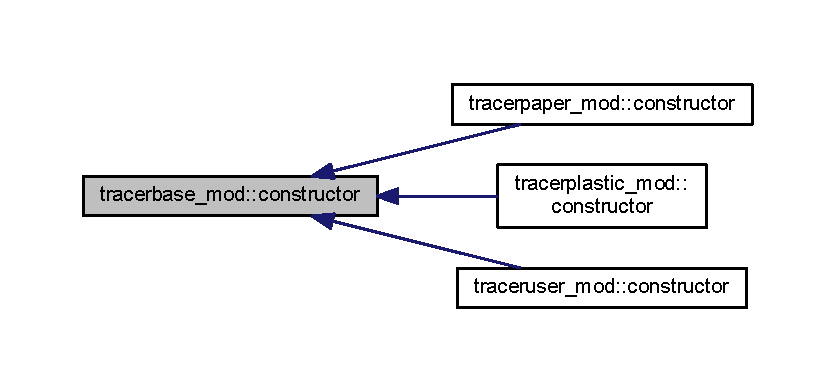
\includegraphics[width=350pt]{namespacetracerbase__mod_aefc12c2007d7598ff9b35733b430a3a2_icgraph}
\end{center}
\end{figure}
\mbox{\Hypertarget{namespacetracerbase__mod_ae320123e374df674769dbd48ba5ef46f}\label{namespacetracerbase__mod_ae320123e374df674769dbd48ba5ef46f}} 
\index{tracerbase\+\_\+mod@{tracerbase\+\_\+mod}!printtracer@{printtracer}}
\index{printtracer@{printtracer}!tracerbase\+\_\+mod@{tracerbase\+\_\+mod}}
\subsubsection{\texorpdfstring{printtracer()}{printtracer()}}
{\footnotesize\ttfamily subroutine tracerbase\+\_\+mod\+::printtracer (\begin{DoxyParamCaption}\item[{class(\mbox{\hyperlink{structtracerbase__mod_1_1tracer__class}{tracer\+\_\+class}}), intent(inout)}]{self }\end{DoxyParamCaption})\hspace{0.3cm}{\ttfamily [private]}}



Method to print basic info about the Tracer. 

\begin{DoxyAuthor}{Author}
Ricardo Birjukovs Canelas -\/ M\+A\+R\+E\+T\+EC 
\end{DoxyAuthor}

\begin{DoxyParams}[1]{Parameters}
\mbox{\tt in}  & {\em self} & \\
\hline
\end{DoxyParams}


Definition at line 76 of file tracer\+Base.\+f90.


\begin{DoxyCode}
76     \textcolor{keywordtype}{implicit none}
77     \textcolor{keywordtype}{class}(tracer\_class), \textcolor{keywordtype}{intent(inout)} :: self
78     \textcolor{keywordtype}{type}(string) :: outext, t(6)
79     \textcolor{keywordflow}{if} (self%now%active .eqv. .false.) \textcolor{keywordflow}{then}
80         outext = \textcolor{stringliteral}{'-->Tracer is inactive'}
81         \textcolor{keyword}{call }log%put(outext,.false.)
82     \textcolor{keywordflow}{else}
83         t(1) = self%par%id
84         t(2) = self%now%pos%x
85         t(3) = self%now%pos%y
86         t(4) = self%now%pos%z
87         outext = \textcolor{stringliteral}{'Tracer['}//t(1)//\textcolor{stringliteral}{']::xyz('}//t(2)//\textcolor{stringliteral}{','}//t(3)//\textcolor{stringliteral}{','}//t(4)//\textcolor{stringliteral}{')'}
88         \textcolor{keyword}{call }log%put(outext,.false.)
89 \textcolor{keywordflow}{    end if}
\end{DoxyCode}

\hypertarget{namespacetracerlist__mod}{}\section{tracerlist\+\_\+mod Module Reference}
\label{namespacetracerlist__mod}\index{tracerlist\+\_\+mod@{tracerlist\+\_\+mod}}


Module to hold the tracer linked list class and its methods. This class defines a double linked list to store any variable type, but with specific methods with type guards for Tracer objects. The class allows for insertion, deletion and iteration of the desired contents.  


\subsection*{Data Types}
\begin{DoxyCompactItemize}
\item 
type \mbox{\hyperlink{structtracerlist__mod_1_1tracerlist__class}{tracerlist\+\_\+class}}
\end{DoxyCompactItemize}
\subsection*{Functions/\+Subroutines}
\begin{DoxyCompactItemize}
\item 
subroutine \mbox{\hyperlink{namespacetracerlist__mod_ae45210a1a3aa4111f97deb5ecf811ca5}{print\+\_\+tracerlist}} (this)
\begin{DoxyCompactList}\small\item\em Method that prints all the links of the list. \end{DoxyCompactList}\item 
subroutine \mbox{\hyperlink{namespacetracerlist__mod_a4476a16f089c0b6e249e7136f73b510c}{print\+\_\+tracerlistcurrent}} (this)
\begin{DoxyCompactList}\small\item\em Method that prints the current link of the list. \end{DoxyCompactList}\end{DoxyCompactItemize}


\subsection{Detailed Description}
Module to hold the tracer linked list class and its methods. This class defines a double linked list to store any variable type, but with specific methods with type guards for Tracer objects. The class allows for insertion, deletion and iteration of the desired contents. 

\begin{DoxyAuthor}{Author}
Ricardo Birjukovs Canelas 
\end{DoxyAuthor}


\subsection{Function/\+Subroutine Documentation}
\mbox{\Hypertarget{namespacetracerlist__mod_ae45210a1a3aa4111f97deb5ecf811ca5}\label{namespacetracerlist__mod_ae45210a1a3aa4111f97deb5ecf811ca5}} 
\index{tracerlist\+\_\+mod@{tracerlist\+\_\+mod}!print\+\_\+tracerlist@{print\+\_\+tracerlist}}
\index{print\+\_\+tracerlist@{print\+\_\+tracerlist}!tracerlist\+\_\+mod@{tracerlist\+\_\+mod}}
\subsubsection{\texorpdfstring{print\+\_\+tracerlist()}{print\_tracerlist()}}
{\footnotesize\ttfamily subroutine tracerlist\+\_\+mod\+::print\+\_\+tracerlist (\begin{DoxyParamCaption}\item[{class(\mbox{\hyperlink{structtracerlist__mod_1_1tracerlist__class}{tracerlist\+\_\+class}}), intent(in)}]{this }\end{DoxyParamCaption})\hspace{0.3cm}{\ttfamily [private]}}



Method that prints all the links of the list. 

\begin{DoxyAuthor}{Author}
Ricardo Birjukovs Canelas -\/ M\+A\+R\+E\+T\+EC 
\end{DoxyAuthor}


Definition at line 83 of file tracer\+List.\+f90.


\begin{DoxyCode}
83     \textcolor{keywordtype}{class}(tracerList\_class), \textcolor{keywordtype}{intent(in)} :: this
84     \textcolor{keywordtype}{class}(*), \textcolor{keywordtype}{pointer} :: curr
85     \textcolor{keywordtype}{type}(string) :: outext
86     outext = this%getSize()
87     outext = \textcolor{stringliteral}{'Tracer list has '}// outext// \textcolor{stringliteral}{' Tracers'}
88     \textcolor{keyword}{call }log%put(outext)
89     \textcolor{keyword}{call }this%reset()               \textcolor{comment}{! reset list iterator}
90     \textcolor{keywordflow}{do} \textcolor{keywordflow}{while}(this%moreValues())     \textcolor{comment}{! loop while there are values to print}
91         \textcolor{keyword}{call }this%printCurrent()
92         \textcolor{keyword}{call }this%next()            \textcolor{comment}{! increment the list iterator}
93 \textcolor{keywordflow}{    end do}
94     \textcolor{keyword}{call }this%reset()               \textcolor{comment}{! reset list iterator}
\end{DoxyCode}
\mbox{\Hypertarget{namespacetracerlist__mod_a4476a16f089c0b6e249e7136f73b510c}\label{namespacetracerlist__mod_a4476a16f089c0b6e249e7136f73b510c}} 
\index{tracerlist\+\_\+mod@{tracerlist\+\_\+mod}!print\+\_\+tracerlistcurrent@{print\+\_\+tracerlistcurrent}}
\index{print\+\_\+tracerlistcurrent@{print\+\_\+tracerlistcurrent}!tracerlist\+\_\+mod@{tracerlist\+\_\+mod}}
\subsubsection{\texorpdfstring{print\+\_\+tracerlistcurrent()}{print\_tracerlistcurrent()}}
{\footnotesize\ttfamily subroutine tracerlist\+\_\+mod\+::print\+\_\+tracerlistcurrent (\begin{DoxyParamCaption}\item[{class(\mbox{\hyperlink{structtracerlist__mod_1_1tracerlist__class}{tracerlist\+\_\+class}}), intent(in)}]{this }\end{DoxyParamCaption})\hspace{0.3cm}{\ttfamily [private]}}



Method that prints the current link of the list. 

\begin{DoxyAuthor}{Author}
Ricardo Birjukovs Canelas -\/ M\+A\+R\+E\+T\+EC 
\end{DoxyAuthor}


Definition at line 103 of file tracer\+List.\+f90.


\begin{DoxyCode}
103     \textcolor{keywordtype}{class}(tracerList\_class), \textcolor{keywordtype}{intent(in)} :: this
104     \textcolor{keywordtype}{class}(*), \textcolor{keywordtype}{pointer} :: curr
105     \textcolor{keywordtype}{type}(string) :: outext
106     curr => this%currentValue() \textcolor{comment}{! get current value}
107     \textcolor{keywordflow}{select type}(curr)
108 \textcolor{keywordflow}{    class is} (tracer\_class)
109         \textcolor{keyword}{call }curr%print()
110 \textcolor{keywordflow}{    class default}
111         outext = \textcolor{stringliteral}{'[tracerList\_class::print] Unexepected type of content, not a Tracer'}
112         \textcolor{keyword}{call }log%put(outext)
113         stop
114 \textcolor{keywordflow}{    end select}
\end{DoxyCode}

\hypertarget{namespacetracerpaper__mod}{}\section{tracerpaper\+\_\+mod Module Reference}
\label{namespacetracerpaper__mod}\index{tracerpaper\+\_\+mod@{tracerpaper\+\_\+mod}}


Module that defines a Lagrangian tracer class for paper modelling and related methods. The type is defined as a derived type from the pule Lagrangian tracer, and hence inherits all of it\textquotesingle{}s data and methods.  


\subsection*{Data Types}
\begin{DoxyCompactItemize}
\item 
type \mbox{\hyperlink{structtracerpaper__mod_1_1paper__class}{paper\+\_\+class}}
\begin{DoxyCompactList}\small\item\em Type -\/ The plastic material Lagrangian tracer class. \end{DoxyCompactList}\item 
type \mbox{\hyperlink{structtracerpaper__mod_1_1paper__par__class}{paper\+\_\+par\+\_\+class}}
\item 
type \mbox{\hyperlink{structtracerpaper__mod_1_1paper__state__class}{paper\+\_\+state\+\_\+class}}
\begin{DoxyCompactList}\small\item\em Type -\/ State variables of a tracer object representing a paper material. \end{DoxyCompactList}\item 
interface \mbox{\hyperlink{interfacetracerpaper__mod_1_1papertracer}{papertracer}}
\end{DoxyCompactItemize}
\subsection*{Functions/\+Subroutines}
\begin{DoxyCompactItemize}
\item 
type(\mbox{\hyperlink{structtracerpaper__mod_1_1paper__class}{paper\+\_\+class}}) function \mbox{\hyperlink{namespacetracerpaper__mod_ad1bbc9d4e889b6aab71f0333cf6a5365}{constructor}} (id, src, time, p)
\begin{DoxyCompactList}\small\item\em Paper Tracer constructor. \end{DoxyCompactList}\end{DoxyCompactItemize}


\subsection{Detailed Description}
Module that defines a Lagrangian tracer class for paper modelling and related methods. The type is defined as a derived type from the pule Lagrangian tracer, and hence inherits all of it\textquotesingle{}s data and methods. 

\begin{DoxyAuthor}{Author}
Ricardo Birjukovs Canelas 
\end{DoxyAuthor}


\subsection{Function/\+Subroutine Documentation}
\mbox{\Hypertarget{namespacetracerpaper__mod_ad1bbc9d4e889b6aab71f0333cf6a5365}\label{namespacetracerpaper__mod_ad1bbc9d4e889b6aab71f0333cf6a5365}} 
\index{tracerpaper\+\_\+mod@{tracerpaper\+\_\+mod}!constructor@{constructor}}
\index{constructor@{constructor}!tracerpaper\+\_\+mod@{tracerpaper\+\_\+mod}}
\subsubsection{\texorpdfstring{constructor()}{constructor()}}
{\footnotesize\ttfamily type(\mbox{\hyperlink{structtracerpaper__mod_1_1paper__class}{paper\+\_\+class}}) function tracerpaper\+\_\+mod\+::constructor (\begin{DoxyParamCaption}\item[{integer, intent(in)}]{id,  }\item[{class(\mbox{\hyperlink{structsources__mod_1_1source__class}{source\+\_\+class}}), intent(in)}]{src,  }\item[{real(prec), intent(in)}]{time,  }\item[{integer, intent(in)}]{p }\end{DoxyParamCaption})\hspace{0.3cm}{\ttfamily [private]}}



Paper Tracer constructor. 

\begin{DoxyAuthor}{Author}
Ricardo Birjukovs Canelas -\/ M\+A\+R\+E\+T\+EC 
\end{DoxyAuthor}

\begin{DoxyParams}[1]{Parameters}
\mbox{\tt in}  & {\em id,src,time,p} & \\
\hline
\end{DoxyParams}


Definition at line 68 of file tracer\+Paper.\+f90.


\begin{DoxyCode}
68     \textcolor{keywordtype}{type}(paper\_class) :: constructor
69     \textcolor{keywordtype}{integer}, \textcolor{keywordtype}{intent(in)} :: id
70     \textcolor{keywordtype}{class}(source\_class), \textcolor{keywordtype}{intent(in)} :: src
71     \textcolor{keywordtype}{real(prec)}, \textcolor{keywordtype}{intent(in)} :: time
72     \textcolor{keywordtype}{integer}, \textcolor{keywordtype}{intent(in)} :: p
73 
74     \textcolor{comment}{!use the base class constructor to build the base of our new derived type}
75     constructor%tracer\_class = tracer(id, src, time, p)
76     \textcolor{comment}{!VERY NICE IFORT BUG (I think) - only some of the variables get used using the base constructor...}
77     constructor%par%id = id \textcolor{comment}{!forcing}
78     constructor%par%idsource = src%par%id \textcolor{comment}{!forcing}
79     \textcolor{comment}{!now initialize the specific components of this derived type}
80     \textcolor{comment}{!material parameters}
81     constructor%mpar%degradation\_rate = src%prop%degrd\_rate
82     constructor%mpar%particulate = src%prop%particulate
83     constructor%mpar%size = src%prop%radius
84     \textcolor{comment}{!material state}
85     constructor%mnow%density = src%prop%density
86     constructor%mnow%condition = src%prop%condition
87     constructor%mnow%radius = src%prop%radius
88     constructor%mnow%concentration = mv
89     \textcolor{keywordflow}{if} (constructor%mpar%particulate) \textcolor{keywordflow}{then}
90         constructor%mpar%size = src%prop%pt\_radius \textcolor{comment}{!correcting size to now mean particle size, not tracer
       size}
91         constructor%mnow%concentration = src%prop%ini\_concentration
92 \textcolor{keywordflow}{    end if}
93 
\end{DoxyCode}
Here is the call graph for this function\+:\nopagebreak
\begin{figure}[H]
\begin{center}
\leavevmode
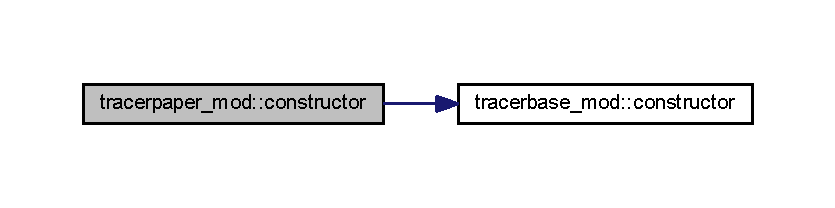
\includegraphics[width=350pt]{namespacetracerpaper__mod_ad1bbc9d4e889b6aab71f0333cf6a5365_cgraph}
\end{center}
\end{figure}

\hypertarget{namespacetracerplastic__mod}{}\section{tracerplastic\+\_\+mod Module Reference}
\label{namespacetracerplastic__mod}\index{tracerplastic\+\_\+mod@{tracerplastic\+\_\+mod}}


Module that defines a Lagrangian tracer class for plastic modelling and related methods. The type is defined as a derived type from the pule Lagrangian tracer, and hence inherits all of it\textquotesingle{}s data and methods.  


\subsection*{Data Types}
\begin{DoxyCompactItemize}
\item 
type \mbox{\hyperlink{structtracerplastic__mod_1_1plastic__class}{plastic\+\_\+class}}
\begin{DoxyCompactList}\small\item\em Type -\/ The plastic material Lagrangian tracer class. \end{DoxyCompactList}\item 
type \mbox{\hyperlink{structtracerplastic__mod_1_1plastic__par__class}{plastic\+\_\+par\+\_\+class}}
\item 
type \mbox{\hyperlink{structtracerplastic__mod_1_1plastic__state__class}{plastic\+\_\+state\+\_\+class}}
\begin{DoxyCompactList}\small\item\em Type -\/ State variables of a tracer object representing a plastic material. \end{DoxyCompactList}\item 
interface \mbox{\hyperlink{interfacetracerplastic__mod_1_1plastictracer}{plastictracer}}
\end{DoxyCompactItemize}
\subsection*{Functions/\+Subroutines}
\begin{DoxyCompactItemize}
\item 
integer function \mbox{\hyperlink{namespacetracerplastic__mod_aa5367c2562d10b5393f263394f07fa49}{getnumvars}} (self)
\begin{DoxyCompactList}\small\item\em Method that returns the number of variables used by this tracer. \end{DoxyCompactList}\item 
real(prec) function, dimension(\+:), allocatable \mbox{\hyperlink{namespacetracerplastic__mod_aa8cdd2196261b216dd6cdd5b7ef2fe90}{getstatearray}} (self)
\begin{DoxyCompactList}\small\item\em Method that returns the state array of this tracer. \end{DoxyCompactList}\item 
subroutine \mbox{\hyperlink{namespacetracerplastic__mod_a5e5bd350455400938950d2129c1f4980}{setstatearray}} (self, state\+Array)
\begin{DoxyCompactList}\small\item\em Method that sets the state array of this tracer. \end{DoxyCompactList}\item 
type(\mbox{\hyperlink{structtracerplastic__mod_1_1plastic__class}{plastic\+\_\+class}}) function \mbox{\hyperlink{namespacetracerplastic__mod_ae68444b860b6e7abf3940b0ee1bfe57a}{constructor}} (id, src, time, p)
\begin{DoxyCompactList}\small\item\em Plastic Tracer constructor. \end{DoxyCompactList}\end{DoxyCompactItemize}


\subsection{Detailed Description}
Module that defines a Lagrangian tracer class for plastic modelling and related methods. The type is defined as a derived type from the pule Lagrangian tracer, and hence inherits all of it\textquotesingle{}s data and methods. 

\begin{DoxyAuthor}{Author}
Ricardo Birjukovs Canelas 
\end{DoxyAuthor}


\subsection{Function/\+Subroutine Documentation}
\mbox{\Hypertarget{namespacetracerplastic__mod_ae68444b860b6e7abf3940b0ee1bfe57a}\label{namespacetracerplastic__mod_ae68444b860b6e7abf3940b0ee1bfe57a}} 
\index{tracerplastic\+\_\+mod@{tracerplastic\+\_\+mod}!constructor@{constructor}}
\index{constructor@{constructor}!tracerplastic\+\_\+mod@{tracerplastic\+\_\+mod}}
\subsubsection{\texorpdfstring{constructor()}{constructor()}}
{\footnotesize\ttfamily type(\mbox{\hyperlink{structtracerplastic__mod_1_1plastic__class}{plastic\+\_\+class}}) function tracerplastic\+\_\+mod\+::constructor (\begin{DoxyParamCaption}\item[{integer, intent(in)}]{id,  }\item[{class(\mbox{\hyperlink{structsources__mod_1_1source__class}{source\+\_\+class}}), intent(in)}]{src,  }\item[{real(prec), intent(in)}]{time,  }\item[{integer, intent(in)}]{p }\end{DoxyParamCaption})\hspace{0.3cm}{\ttfamily [private]}}



Plastic Tracer constructor. 

\begin{DoxyAuthor}{Author}
Ricardo Birjukovs Canelas -\/ M\+A\+R\+E\+T\+EC 
\end{DoxyAuthor}

\begin{DoxyParams}[1]{Parameters}
\mbox{\tt in}  & {\em id,src,time,p} & \\
\hline
\end{DoxyParams}


Definition at line 135 of file tracer\+Plastic.\+f90.


\begin{DoxyCode}
135     \textcolor{keywordtype}{type}(plastic\_class) :: constructor
136     \textcolor{keywordtype}{integer}, \textcolor{keywordtype}{intent(in)} :: id
137     \textcolor{keywordtype}{class}(source\_class), \textcolor{keywordtype}{intent(in)} :: src
138     \textcolor{keywordtype}{real(prec)}, \textcolor{keywordtype}{intent(in)} :: time
139     \textcolor{keywordtype}{integer}, \textcolor{keywordtype}{intent(in)} :: p
140     \textcolor{keywordtype}{integer} :: idx
141     \textcolor{keywordtype}{type}(string) :: tag
142 
143     \textcolor{comment}{!use the base class constructor to build the base of our new derived type}
144     constructor%tracer\_class = tracer(id, src, time, p, constructor%getNumVars())
145     \textcolor{comment}{!VERY NICE IFORT BUG (I think) - only some of the variables get used using the base constructor...}
146     constructor%par%id = id \textcolor{comment}{!forcing}
147     constructor%par%idsource = src%par%id \textcolor{comment}{!forcing}
148 
149     \textcolor{comment}{!now initialize the specific components of this derived type}
150     constructor%par%ttype = globals%Types%plastic
151     constructor%mpar%particulate = src%prop%particulate
152     constructor%mpar%size = src%prop%radius
153     \textcolor{comment}{!material state}
154     constructor%mnow%density = src%prop%density
155     constructor%mnow%radius = src%prop%radius
156     \textcolor{comment}{!constructor%mnow%concentration = MV}
157     \textcolor{comment}{!default values}
158     constructor%mnow%condition = 1.0
159     constructor%mnow%degradation\_rate = 1/(100*365*24*3600)
160     \textcolor{comment}{!try to find value from material types files}
161     tag = \textcolor{stringliteral}{'condition'}
162     idx = utils%find\_str(src%prop%propName, tag, .false.)
163     \textcolor{keywordflow}{if} (idx /= mv\_int) \textcolor{keywordflow}{then}
164         constructor%mnow%condition = src%prop%propValue(idx)
165 \textcolor{keywordflow}{    end if}
166     tag = \textcolor{stringliteral}{'degradation\_rate'}
167     idx = utils%find\_str(src%prop%propName, tag, .false.)
168     \textcolor{keywordflow}{if} (idx /= mv\_int) \textcolor{keywordflow}{then}
169         constructor%mnow%degradation\_rate = src%prop%propValue(idx)
170 \textcolor{keywordflow}{    end if}
171 
172     \textcolor{keywordflow}{if} (constructor%mpar%particulate) \textcolor{keywordflow}{then}
173         \textcolor{comment}{!constructor%mpar%size = src%prop%pt\_radius !correcting size to now mean particle size, not tracer
       size}
174         \textcolor{comment}{!constructor%mnow%concentration = src%prop%ini\_concentration}
175 \textcolor{keywordflow}{    end if}
176     
177     \textcolor{comment}{!filling the rest of the varName list}
178     constructor%varName(12) = globals%Var%density
179     constructor%varName(13) = \textcolor{stringliteral}{'radius'}
180     constructor%varName(14) = \textcolor{stringliteral}{'condition'}
181     constructor%varName(15) = \textcolor{stringliteral}{'degradation\_rate'}
182     constructor%varName(16) = \textcolor{stringliteral}{'concentration'}
\end{DoxyCode}
Here is the call graph for this function\+:\nopagebreak
\begin{figure}[H]
\begin{center}
\leavevmode
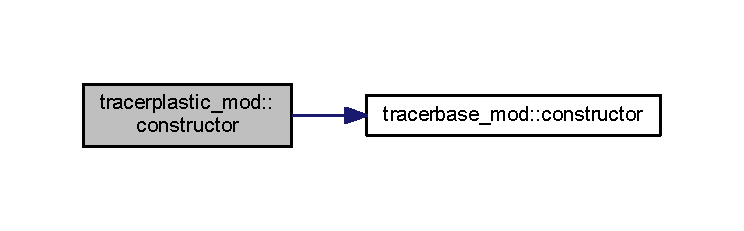
\includegraphics[width=350pt]{namespacetracerplastic__mod_ae68444b860b6e7abf3940b0ee1bfe57a_cgraph}
\end{center}
\end{figure}
\mbox{\Hypertarget{namespacetracerplastic__mod_aa5367c2562d10b5393f263394f07fa49}\label{namespacetracerplastic__mod_aa5367c2562d10b5393f263394f07fa49}} 
\index{tracerplastic\+\_\+mod@{tracerplastic\+\_\+mod}!getnumvars@{getnumvars}}
\index{getnumvars@{getnumvars}!tracerplastic\+\_\+mod@{tracerplastic\+\_\+mod}}
\subsubsection{\texorpdfstring{getnumvars()}{getnumvars()}}
{\footnotesize\ttfamily integer function tracerplastic\+\_\+mod\+::getnumvars (\begin{DoxyParamCaption}\item[{class(\mbox{\hyperlink{structtracerplastic__mod_1_1plastic__class}{plastic\+\_\+class}}), intent(in)}]{self }\end{DoxyParamCaption})\hspace{0.3cm}{\ttfamily [private]}}



Method that returns the number of variables used by this tracer. 

\begin{DoxyAuthor}{Author}
Ricardo Birjukovs Canelas -\/ M\+A\+R\+E\+T\+EC 
\end{DoxyAuthor}


Definition at line 70 of file tracer\+Plastic.\+f90.


\begin{DoxyCode}
70     \textcolor{keywordtype}{class}(plastic\_class), \textcolor{keywordtype}{intent(in)} :: self
71     getnumvars = 16
\end{DoxyCode}
Here is the call graph for this function\+:\nopagebreak
\begin{figure}[H]
\begin{center}
\leavevmode
\includegraphics[width=350pt]{namespacetracerplastic__mod_aa5367c2562d10b5393f263394f07fa49_cgraph}
\end{center}
\end{figure}
\mbox{\Hypertarget{namespacetracerplastic__mod_aa8cdd2196261b216dd6cdd5b7ef2fe90}\label{namespacetracerplastic__mod_aa8cdd2196261b216dd6cdd5b7ef2fe90}} 
\index{tracerplastic\+\_\+mod@{tracerplastic\+\_\+mod}!getstatearray@{getstatearray}}
\index{getstatearray@{getstatearray}!tracerplastic\+\_\+mod@{tracerplastic\+\_\+mod}}
\subsubsection{\texorpdfstring{getstatearray()}{getstatearray()}}
{\footnotesize\ttfamily real(prec) function, dimension(\+:), allocatable tracerplastic\+\_\+mod\+::getstatearray (\begin{DoxyParamCaption}\item[{class(\mbox{\hyperlink{structtracerplastic__mod_1_1plastic__class}{plastic\+\_\+class}}), intent(in)}]{self }\end{DoxyParamCaption})\hspace{0.3cm}{\ttfamily [private]}}



Method that returns the state array of this tracer. 

\begin{DoxyAuthor}{Author}
Ricardo Birjukovs Canelas -\/ M\+A\+R\+E\+T\+EC 
\end{DoxyAuthor}


Definition at line 80 of file tracer\+Plastic.\+f90.


\begin{DoxyCode}
80     \textcolor{keywordtype}{class}(plastic\_class), \textcolor{keywordtype}{intent(in)} :: self
81     \textcolor{keywordtype}{real(prec)}, \textcolor{keywordtype}{allocatable}, \textcolor{keywordtype}{dimension(:)} :: getStateArray
82     \textcolor{keyword}{allocate}(getstatearray(self%getNumVars()))
83     getstatearray(1) = self%now%pos%x
84     getstatearray(2) = self%now%pos%y
85     getstatearray(3) = self%now%pos%z
86     getstatearray(4) = self%now%vel%x
87     getstatearray(5) = self%now%vel%y
88     getstatearray(6) = self%now%vel%z
89     getstatearray(7) = self%now%diffusionVel%x
90     getstatearray(8) = self%now%diffusionVel%y
91     getstatearray(9) = self%now%diffusionVel%z
92     getstatearray(10) = self%now%usedMixingLenght
93     getstatearray(11) = self%now%age
94     getstatearray(12) = self%mnow%density
95     getstatearray(13) = self%mnow%radius
96     getstatearray(14) = self%mnow%condition
97     getstatearray(15) = self%mnow%degradation\_rate
98     getstatearray(16) = self%mnow%concentration
\end{DoxyCode}
Here is the call graph for this function\+:\nopagebreak
\begin{figure}[H]
\begin{center}
\leavevmode
\includegraphics[width=350pt]{namespacetracerplastic__mod_aa8cdd2196261b216dd6cdd5b7ef2fe90_cgraph}
\end{center}
\end{figure}
\mbox{\Hypertarget{namespacetracerplastic__mod_a5e5bd350455400938950d2129c1f4980}\label{namespacetracerplastic__mod_a5e5bd350455400938950d2129c1f4980}} 
\index{tracerplastic\+\_\+mod@{tracerplastic\+\_\+mod}!setstatearray@{setstatearray}}
\index{setstatearray@{setstatearray}!tracerplastic\+\_\+mod@{tracerplastic\+\_\+mod}}
\subsubsection{\texorpdfstring{setstatearray()}{setstatearray()}}
{\footnotesize\ttfamily subroutine tracerplastic\+\_\+mod\+::setstatearray (\begin{DoxyParamCaption}\item[{class(\mbox{\hyperlink{structtracerplastic__mod_1_1plastic__class}{plastic\+\_\+class}}), intent(inout)}]{self,  }\item[{real(prec), dimension(\+:), intent(in)}]{state\+Array }\end{DoxyParamCaption})\hspace{0.3cm}{\ttfamily [private]}}



Method that sets the state array of this tracer. 

\begin{DoxyAuthor}{Author}
Ricardo Birjukovs Canelas -\/ M\+A\+R\+E\+T\+EC 
\end{DoxyAuthor}


Definition at line 107 of file tracer\+Plastic.\+f90.


\begin{DoxyCode}
107     \textcolor{keywordtype}{class}(plastic\_class), \textcolor{keywordtype}{intent(inout)} :: self
108     \textcolor{keywordtype}{real(prec)}, \textcolor{keywordtype}{dimension(:)}, \textcolor{keywordtype}{intent(in)} :: stateArray
109     \textcolor{comment}{!if(size(stateArray)<self%getNumVars())}
110     self%now%pos%x = statearray(1)
111     self%now%pos%y = statearray(2)
112     self%now%pos%z = statearray(3)
113     self%now%vel%x = statearray(4)
114     self%now%vel%y = statearray(5)
115     self%now%vel%z = statearray(6)
116     self%now%diffusionVel%z = statearray(7)
117     self%now%diffusionVel%z = statearray(8)
118     self%now%diffusionVel%z = statearray(9)
119     self%now%usedMixingLenght = statearray(10)
120     self%now%age   = statearray(11)
121     self%mnow%density = statearray(12)
122     self%mnow%radius = statearray(13)
123     self%mnow%condition = statearray(14)
124     self%mnow%degradation\_rate = statearray(15)
125     self%mnow%concentration = statearray(16)
\end{DoxyCode}

\hypertarget{namespacetracers__mod}{}\section{tracers\+\_\+mod Module Reference}
\label{namespacetracers__mod}\index{tracers\+\_\+mod@{tracers\+\_\+mod}}


Module to hold and \textquotesingle{}wrap\textquotesingle{} all the tracer respective modules.  




\subsection{Detailed Description}
Module to hold and \textquotesingle{}wrap\textquotesingle{} all the tracer respective modules. 

\begin{DoxyAuthor}{Author}
Ricardo Birjukovs Canelas 
\end{DoxyAuthor}

\hypertarget{namespacetraceruser__mod}{}\section{traceruser\+\_\+mod Module Reference}
\label{namespacetraceruser__mod}\index{traceruser\+\_\+mod@{traceruser\+\_\+mod}}


Module that defines a generic Lagrangian tracer class for material modelling and related methods. The type is defined as a derived type from the pule Lagrangian tracer, and hence inherits all of it\textquotesingle{}s data and methods. It holds an arbitrarily sized array for properties and their names, that a user can then explore in the methods.  


\subsection*{Data Types}
\begin{DoxyCompactItemize}
\item 
type \mbox{\hyperlink{structtraceruser__mod_1_1user__par__class}{user\+\_\+par\+\_\+class}}
\item 
type \mbox{\hyperlink{structtraceruser__mod_1_1user__state__class}{user\+\_\+state\+\_\+class}}
\begin{DoxyCompactList}\small\item\em Type -\/ State variables of a tracer object representing a user defined type. \end{DoxyCompactList}\item 
interface \mbox{\hyperlink{interfacetraceruser__mod_1_1usertracer}{usertracer}}
\item 
type \mbox{\hyperlink{structtraceruser__mod_1_1usertracer__class}{usertracer\+\_\+class}}
\begin{DoxyCompactList}\small\item\em Type -\/ The user-\/defined Lagrangian tracer class. \end{DoxyCompactList}\end{DoxyCompactItemize}
\subsection*{Functions/\+Subroutines}
\begin{DoxyCompactItemize}
\item 
type(\mbox{\hyperlink{structtraceruser__mod_1_1usertracer__class}{usertracer\+\_\+class}}) function \mbox{\hyperlink{namespacetraceruser__mod_a9b5d52bbc9611921275ff35fa82a91c5}{constructor}} (id, src, time, p)
\begin{DoxyCompactList}\small\item\em User-\/defined Tracer constructor. \end{DoxyCompactList}\end{DoxyCompactItemize}


\subsection{Detailed Description}
Module that defines a generic Lagrangian tracer class for material modelling and related methods. The type is defined as a derived type from the pule Lagrangian tracer, and hence inherits all of it\textquotesingle{}s data and methods. It holds an arbitrarily sized array for properties and their names, that a user can then explore in the methods. 

\begin{DoxyAuthor}{Author}
Ricardo Birjukovs Canelas 
\end{DoxyAuthor}


\subsection{Function/\+Subroutine Documentation}
\mbox{\Hypertarget{namespacetraceruser__mod_a9b5d52bbc9611921275ff35fa82a91c5}\label{namespacetraceruser__mod_a9b5d52bbc9611921275ff35fa82a91c5}} 
\index{traceruser\+\_\+mod@{traceruser\+\_\+mod}!constructor@{constructor}}
\index{constructor@{constructor}!traceruser\+\_\+mod@{traceruser\+\_\+mod}}
\subsubsection{\texorpdfstring{constructor()}{constructor()}}
{\footnotesize\ttfamily type(\mbox{\hyperlink{structtraceruser__mod_1_1usertracer__class}{usertracer\+\_\+class}}) function traceruser\+\_\+mod\+::constructor (\begin{DoxyParamCaption}\item[{integer, intent(in)}]{id,  }\item[{class(\mbox{\hyperlink{structsources__mod_1_1source__class}{source\+\_\+class}}), intent(in)}]{src,  }\item[{real(prec), intent(in)}]{time,  }\item[{integer, intent(in)}]{p }\end{DoxyParamCaption})\hspace{0.3cm}{\ttfamily [private]}}



User-\/defined Tracer constructor. 

\begin{DoxyAuthor}{Author}
Ricardo Birjukovs Canelas -\/ M\+A\+R\+E\+T\+EC 
\end{DoxyAuthor}

\begin{DoxyParams}[1]{Parameters}
\mbox{\tt in}  & {\em id,src,time,p} & \\
\hline
\end{DoxyParams}


Definition at line 68 of file tracer\+User.\+f90.


\begin{DoxyCode}
68     \textcolor{keywordtype}{type}(userTracer\_class) :: constructor
69     \textcolor{keywordtype}{integer}, \textcolor{keywordtype}{intent(in)} :: id
70     \textcolor{keywordtype}{class}(source\_class), \textcolor{keywordtype}{intent(in)} :: src
71     \textcolor{keywordtype}{real(prec)}, \textcolor{keywordtype}{intent(in)} :: time
72     \textcolor{keywordtype}{integer}, \textcolor{keywordtype}{intent(in)} :: p
73 
74     \textcolor{comment}{!use the base class constructor to build the base of our new derived type}
75     constructor%tracer\_class = tracer(id, src, time, p)
76     \textcolor{comment}{!VERY NICE IFORT BUG (I think) - only some of the variables get used using the base constructor...}
77     constructor%par%id = id \textcolor{comment}{!forcing}
78     constructor%par%idsource = src%par%id \textcolor{comment}{!forcing}
79     \textcolor{comment}{!now initialize the specific components of this derived type}
80 
\end{DoxyCode}
Here is the call graph for this function\+:\nopagebreak
\begin{figure}[H]
\begin{center}
\leavevmode
\includegraphics[width=350pt]{namespacetraceruser__mod_a9b5d52bbc9611921275ff35fa82a91c5_cgraph}
\end{center}
\end{figure}

\hypertarget{namespaceutilities__mod}{}\section{utilities\+\_\+mod Module Reference}
\label{namespaceutilities__mod}\index{utilities\+\_\+mod@{utilities\+\_\+mod}}


Module that provides useful back-\/end routines.  


\subsection*{Data Types}
\begin{DoxyCompactItemize}
\item 
type \mbox{\hyperlink{structutilities__mod_1_1utils__class}{utils\+\_\+class}}
\end{DoxyCompactItemize}
\subsection*{Functions/\+Subroutines}
\begin{DoxyCompactItemize}
\item 
integer function, dimension(6) \mbox{\hyperlink{namespaceutilities__mod_ab5b97f243f9347a40db76d55509d37ca}{getdatefromisostring}} (self, date\+Str)
\begin{DoxyCompactList}\small\item\em Function that returns an integer array of type (year, month, day, hour, minute, second) from an I\+SO date string. \end{DoxyCompactList}\item 
integer function \mbox{\hyperlink{namespaceutilities__mod_ad446cce78a6509db0e839439a0e84564}{find\+\_\+str}} (self, str\+\_\+array, str, mandatory)
\begin{DoxyCompactList}\small\item\em returns the index of a given string in an array of strings. Has optional mandatory flag. \end{DoxyCompactList}\item 
type(vector) function \mbox{\hyperlink{namespaceutilities__mod_ad6e463f7e5fc49fe4fcd5464326ade01}{geo2m}} (self, geovec, lat)
\begin{DoxyCompactList}\small\item\em Returns a vector in meters given an array in geographical coordinates (lon, lat, z) and a lattitude. \end{DoxyCompactList}\item 
type(vector) function \mbox{\hyperlink{namespaceutilities__mod_a70b21b18c8633b7fd4c3057530d3f16f}{m2geo\+\_\+vec}} (self, mvec, lat)
\begin{DoxyCompactList}\small\item\em Returns a vector in geographical coordinates (lon, lat, z) given an array in meters and a lattitude. \end{DoxyCompactList}\item 
real(prec) function, dimension(size(mvec)) \mbox{\hyperlink{namespaceutilities__mod_ae6b8a45b229e3f1f8c2b12dd74e7a2dd}{m2geo\+\_\+comp}} (self, mvec, lat, component)
\begin{DoxyCompactList}\small\item\em Returns a vector in geographical coordinates (lon, lat, z) given an array in meters and a lattitude. \end{DoxyCompactList}\item 
character(\+:) function, allocatable \mbox{\hyperlink{namespaceutilities__mod_a6ba00b0a503f26c7e755d1efbbe83c5b}{int2str}} (self, fmt, i)
\begin{DoxyCompactList}\small\item\em Returns a zero paded string from an integer number and a format descriptor. \end{DoxyCompactList}\item 
real(prec) function \mbox{\hyperlink{namespaceutilities__mod_a164054d89c012d95f63c12a6cc0ac8d7}{get\+\_\+closest\+\_\+twopow}} (self, num)
\begin{DoxyCompactList}\small\item\em Returns the closest power of 2 or a given real number. \end{DoxyCompactList}\end{DoxyCompactItemize}
\subsection*{Variables}
\begin{DoxyCompactItemize}
\item 
type(\mbox{\hyperlink{structutilities__mod_1_1utils__class}{utils\+\_\+class}}), public \mbox{\hyperlink{namespaceutilities__mod_aa12c2506b3107528a2511d059186f12d}{utils}}
\end{DoxyCompactItemize}


\subsection{Detailed Description}
Module that provides useful back-\/end routines. 

\begin{DoxyAuthor}{Author}
Ricardo Birjukovs Canelas 
\end{DoxyAuthor}


\subsection{Function/\+Subroutine Documentation}
\mbox{\Hypertarget{namespaceutilities__mod_ad446cce78a6509db0e839439a0e84564}\label{namespaceutilities__mod_ad446cce78a6509db0e839439a0e84564}} 
\index{utilities\+\_\+mod@{utilities\+\_\+mod}!find\+\_\+str@{find\+\_\+str}}
\index{find\+\_\+str@{find\+\_\+str}!utilities\+\_\+mod@{utilities\+\_\+mod}}
\subsubsection{\texorpdfstring{find\+\_\+str()}{find\_str()}}
{\footnotesize\ttfamily integer function utilities\+\_\+mod\+::find\+\_\+str (\begin{DoxyParamCaption}\item[{class(\mbox{\hyperlink{structutilities__mod_1_1utils__class}{utils\+\_\+class}}), intent(in)}]{self,  }\item[{type(string), dimension(\+:), intent(in)}]{str\+\_\+array,  }\item[{type(string), intent(in)}]{str,  }\item[{logical, intent(in), optional}]{mandatory }\end{DoxyParamCaption})\hspace{0.3cm}{\ttfamily [private]}}



returns the index of a given string in an array of strings. Has optional mandatory flag. 

\begin{DoxyAuthor}{Author}
Ricardo Birjukovs Canelas -\/ M\+A\+R\+E\+T\+EC 
\end{DoxyAuthor}

\begin{DoxyParams}[1]{Parameters}
\mbox{\tt in}  & {\em self,str\+\_\+array,str,mandatory} & \\
\hline
\end{DoxyParams}


Definition at line 82 of file utilities.\+f90.


\begin{DoxyCode}
82     \textcolor{keywordtype}{class}(utils\_class), \textcolor{keywordtype}{intent(in)} :: self
83     \textcolor{keywordtype}{type}(string), \textcolor{keywordtype}{dimension(:)}, \textcolor{keywordtype}{intent(in)} :: str\_array
84     \textcolor{keywordtype}{type}(string), \textcolor{keywordtype}{intent(in)} :: str
85     \textcolor{keywordtype}{logical}, \textcolor{keywordtype}{optional}, \textcolor{keywordtype}{intent(in)} :: mandatory
86     \textcolor{keywordtype}{type}(string) :: outext
87     \textcolor{keywordflow}{do} find\_str=1, \textcolor{keyword}{size}(str\_array)
88         \textcolor{keywordflow}{if} (str == str\_array(find\_str)) \textcolor{keywordflow}{return}
89 \textcolor{keywordflow}{    end do}
90     \textcolor{keywordflow}{if}(\textcolor{keyword}{present}(mandatory)) \textcolor{keywordflow}{then}
91         \textcolor{keywordflow}{if} (mandatory) \textcolor{keywordflow}{then}
92             outext = \textcolor{stringliteral}{'[Utils::find\_str]: string "'}// str //\textcolor{stringliteral}{'" not found on list, stopping'}
93             \textcolor{keyword}{call }log%put(outext)
94             stop
95 \textcolor{keywordflow}{        end if}
96 \textcolor{keywordflow}{    end if}
\end{DoxyCode}
\mbox{\Hypertarget{namespaceutilities__mod_ad6e463f7e5fc49fe4fcd5464326ade01}\label{namespaceutilities__mod_ad6e463f7e5fc49fe4fcd5464326ade01}} 
\index{utilities\+\_\+mod@{utilities\+\_\+mod}!geo2m@{geo2m}}
\index{geo2m@{geo2m}!utilities\+\_\+mod@{utilities\+\_\+mod}}
\subsubsection{\texorpdfstring{geo2m()}{geo2m()}}
{\footnotesize\ttfamily type(vector) function utilities\+\_\+mod\+::geo2m (\begin{DoxyParamCaption}\item[{class(\mbox{\hyperlink{structutilities__mod_1_1utils__class}{utils\+\_\+class}}), intent(in)}]{self,  }\item[{type(vector), intent(in)}]{geovec,  }\item[{real(prec), intent(in)}]{lat }\end{DoxyParamCaption})\hspace{0.3cm}{\ttfamily [private]}}



Returns a vector in meters given an array in geographical coordinates (lon, lat, z) and a lattitude. 

\begin{DoxyAuthor}{Author}
Ricardo Birjukovs Canelas -\/ M\+A\+R\+E\+T\+EC 
\end{DoxyAuthor}

\begin{DoxyParams}[1]{Parameters}
\mbox{\tt in}  & {\em self,geovec,lat} & \\
\hline
\end{DoxyParams}


Definition at line 107 of file utilities.\+f90.


\begin{DoxyCode}
107     \textcolor{keywordtype}{class}(utils\_class), \textcolor{keywordtype}{intent(in)} :: self
108     \textcolor{keywordtype}{type}(vector), \textcolor{keywordtype}{intent(in)} :: geovec
109     \textcolor{keywordtype}{real(prec)}, \textcolor{keywordtype}{intent(in)} :: lat
110     \textcolor{keywordtype}{integer} :: R
111     \textcolor{keywordtype}{real(prec)} :: pi = 4*atan(1.0)
112     r = 6378137 \textcolor{comment}{!earth radius in meters}
113     \textcolor{comment}{!pi = 3.1415926}
114     res = geovec
115     res%x = res%x*r*cos(pi*lat/180.0)
116     res%y = res%y*r
\end{DoxyCode}
\mbox{\Hypertarget{namespaceutilities__mod_a164054d89c012d95f63c12a6cc0ac8d7}\label{namespaceutilities__mod_a164054d89c012d95f63c12a6cc0ac8d7}} 
\index{utilities\+\_\+mod@{utilities\+\_\+mod}!get\+\_\+closest\+\_\+twopow@{get\+\_\+closest\+\_\+twopow}}
\index{get\+\_\+closest\+\_\+twopow@{get\+\_\+closest\+\_\+twopow}!utilities\+\_\+mod@{utilities\+\_\+mod}}
\subsubsection{\texorpdfstring{get\+\_\+closest\+\_\+twopow()}{get\_closest\_twopow()}}
{\footnotesize\ttfamily real(prec) function utilities\+\_\+mod\+::get\+\_\+closest\+\_\+twopow (\begin{DoxyParamCaption}\item[{class(\mbox{\hyperlink{structutilities__mod_1_1utils__class}{utils\+\_\+class}}), intent(in)}]{self,  }\item[{real(prec), intent(in)}]{num }\end{DoxyParamCaption})\hspace{0.3cm}{\ttfamily [private]}}



Returns the closest power of 2 or a given real number. 

\begin{DoxyAuthor}{Author}
Ricardo Birjukovs Canelas -\/ M\+A\+R\+E\+T\+EC 
\end{DoxyAuthor}

\begin{DoxyParams}[1]{Parameters}
\mbox{\tt in}  & {\em self,num} & \\
\hline
\end{DoxyParams}


Definition at line 187 of file utilities.\+f90.


\begin{DoxyCode}
187     \textcolor{keywordtype}{class}(utils\_class), \textcolor{keywordtype}{intent(in)} :: self
188     \textcolor{keywordtype}{real(prec)}, \textcolor{keywordtype}{intent(in)} :: num
189     \textcolor{keywordtype}{real(prec)} :: twopow
190     \textcolor{keywordtype}{integer} :: i
191     \textcolor{keywordtype}{real(prec)} :: dist1, dist2
192     \textcolor{keywordflow}{do} i=-4, 10
193         twopow = 2.0**i
194         \textcolor{keywordflow}{if} (num < twopow) \textcolor{keywordflow}{then}
195             dist1 = sqrt(twopow-num)
196             dist2 = sqrt(num-2.0**(i-1))
197             \textcolor{keywordflow}{if} (dist2 < dist1) \textcolor{keywordflow}{then}
198                 twopow = 2.0**(i-1)
199                 \textcolor{keywordflow}{exit}
200 \textcolor{keywordflow}{            endif}
201             \textcolor{keywordflow}{exit}
202 \textcolor{keywordflow}{        endif}
203 \textcolor{keywordflow}{    enddo}
\end{DoxyCode}
\mbox{\Hypertarget{namespaceutilities__mod_ab5b97f243f9347a40db76d55509d37ca}\label{namespaceutilities__mod_ab5b97f243f9347a40db76d55509d37ca}} 
\index{utilities\+\_\+mod@{utilities\+\_\+mod}!getdatefromisostring@{getdatefromisostring}}
\index{getdatefromisostring@{getdatefromisostring}!utilities\+\_\+mod@{utilities\+\_\+mod}}
\subsubsection{\texorpdfstring{getdatefromisostring()}{getdatefromisostring()}}
{\footnotesize\ttfamily integer function, dimension(6) utilities\+\_\+mod\+::getdatefromisostring (\begin{DoxyParamCaption}\item[{class(\mbox{\hyperlink{structutilities__mod_1_1utils__class}{utils\+\_\+class}}), intent(in)}]{self,  }\item[{type(string), intent(in)}]{date\+Str }\end{DoxyParamCaption})\hspace{0.3cm}{\ttfamily [private]}}



Function that returns an integer array of type (year, month, day, hour, minute, second) from an I\+SO date string. 

\begin{DoxyAuthor}{Author}
Ricardo Birjukovs Canelas -\/ M\+A\+R\+E\+T\+EC 
\end{DoxyAuthor}

\begin{DoxyParams}[1]{Parameters}
\mbox{\tt in}  & {\em self,date\+Str} & \\
\hline
\end{DoxyParams}


Definition at line 56 of file utilities.\+f90.


\begin{DoxyCode}
56     \textcolor{keywordtype}{class}(utils\_class), \textcolor{keywordtype}{intent(in)} :: self
57     \textcolor{keywordtype}{type}(string), \textcolor{keywordtype}{intent(in)} :: dateStr
58     \textcolor{keywordtype}{integer}, \textcolor{keywordtype}{dimension(6)} :: getDateFromISOString
59     \textcolor{keywordtype}{integer} :: i
60     \textcolor{keywordtype}{type}(string), \textcolor{keywordtype}{allocatable} :: dc(:)
61     \textcolor{keywordtype}{type}(string) :: outext
62     \textcolor{keyword}{call }datestr%split(tokens=dc, sep=\textcolor{stringliteral}{' '})
63     \textcolor{keywordflow}{if} (\textcolor{keyword}{size}(dc) == 6) \textcolor{keywordflow}{then}
64         \textcolor{keywordflow}{do} i=1, \textcolor{keyword}{size}(dc)
65             getdatefromisostring(i) = dc(i)%to\_number(kind=1.\_r4p)
66 \textcolor{keywordflow}{        end do}
67     \textcolor{keywordflow}{else}
68         outext = \textcolor{stringliteral}{'[Utils::getDateFromISOString] Date '}// datestr //\textcolor{stringliteral}{' not in correct format. Eg. "2009 3 1 0
       0 0"'}
69         \textcolor{keyword}{call }log%put(outext)
70         stop
71 \textcolor{keywordflow}{    end if}    
\end{DoxyCode}
\mbox{\Hypertarget{namespaceutilities__mod_a6ba00b0a503f26c7e755d1efbbe83c5b}\label{namespaceutilities__mod_a6ba00b0a503f26c7e755d1efbbe83c5b}} 
\index{utilities\+\_\+mod@{utilities\+\_\+mod}!int2str@{int2str}}
\index{int2str@{int2str}!utilities\+\_\+mod@{utilities\+\_\+mod}}
\subsubsection{\texorpdfstring{int2str()}{int2str()}}
{\footnotesize\ttfamily character(\+:) function, allocatable utilities\+\_\+mod\+::int2str (\begin{DoxyParamCaption}\item[{class(\mbox{\hyperlink{structutilities__mod_1_1utils__class}{utils\+\_\+class}}), intent(in)}]{self,  }\item[{character(len=6), intent(in)}]{fmt,  }\item[{integer, intent(in)}]{i }\end{DoxyParamCaption})\hspace{0.3cm}{\ttfamily [private]}}



Returns a zero paded string from an integer number and a format descriptor. 

\begin{DoxyAuthor}{Author}
Ricardo Birjukovs Canelas -\/ M\+A\+R\+E\+T\+EC 
\end{DoxyAuthor}

\begin{DoxyParams}[1]{Parameters}
\mbox{\tt in}  & {\em self,fmt,i} & \\
\hline
\end{DoxyParams}


Definition at line 171 of file utilities.\+f90.


\begin{DoxyCode}
171     \textcolor{keywordtype}{class}(utils\_class), \textcolor{keywordtype}{intent(in)} :: self
172     \textcolor{keywordtype}{character(:)}, \textcolor{keywordtype}{allocatable} :: res
173     \textcolor{keywordtype}{character(len=6)}, \textcolor{keywordtype}{intent(in)} :: fmt \textcolor{comment}{! format descriptor}
174     \textcolor{keywordtype}{integer}, \textcolor{keywordtype}{intent(in)} :: i
175     \textcolor{keywordtype}{character(range(i)+2)} :: tmp
176     \textcolor{keyword}{write}(tmp, fmt) i
177     res = trim(tmp)
\end{DoxyCode}
\mbox{\Hypertarget{namespaceutilities__mod_ae6b8a45b229e3f1f8c2b12dd74e7a2dd}\label{namespaceutilities__mod_ae6b8a45b229e3f1f8c2b12dd74e7a2dd}} 
\index{utilities\+\_\+mod@{utilities\+\_\+mod}!m2geo\+\_\+comp@{m2geo\+\_\+comp}}
\index{m2geo\+\_\+comp@{m2geo\+\_\+comp}!utilities\+\_\+mod@{utilities\+\_\+mod}}
\subsubsection{\texorpdfstring{m2geo\+\_\+comp()}{m2geo\_comp()}}
{\footnotesize\ttfamily real(prec) function, dimension(size(mvec)) utilities\+\_\+mod\+::m2geo\+\_\+comp (\begin{DoxyParamCaption}\item[{class(\mbox{\hyperlink{structutilities__mod_1_1utils__class}{utils\+\_\+class}}), intent(in)}]{self,  }\item[{real(prec), dimension(\+:), intent(in)}]{mvec,  }\item[{real(prec), dimension(\+:), intent(in)}]{lat,  }\item[{logical, intent(in)}]{component }\end{DoxyParamCaption})\hspace{0.3cm}{\ttfamily [private]}}



Returns a vector in geographical coordinates (lon, lat, z) given an array in meters and a lattitude. 

\begin{DoxyAuthor}{Author}
Ricardo Birjukovs Canelas -\/ M\+A\+R\+E\+T\+EC 
\end{DoxyAuthor}

\begin{DoxyParams}[1]{Parameters}
\mbox{\tt in}  & {\em self,mvec,lat} & \\
\hline
\end{DoxyParams}


Definition at line 147 of file utilities.\+f90.


\begin{DoxyCode}
147     \textcolor{keywordtype}{class}(utils\_class), \textcolor{keywordtype}{intent(in)} :: self
148     \textcolor{keywordtype}{real(prec)}, \textcolor{keywordtype}{dimension(:)}, \textcolor{keywordtype}{intent(in)} :: mvec    
149     \textcolor{keywordtype}{real(prec)}, \textcolor{keywordtype}{dimension(:)}, \textcolor{keywordtype}{intent(in)} :: lat
150     \textcolor{keywordtype}{logical}, \textcolor{keywordtype}{intent(in)} :: component
151     \textcolor{keywordtype}{real(prec)}, \textcolor{keywordtype}{dimension(size(mvec))} :: m2geo\_comp
152     \textcolor{keywordtype}{real(prec)} :: R
153     \textcolor{keywordtype}{real(prec)} :: pi = 4*atan(1.0)
154     r = 6378137.0 \textcolor{comment}{!earth radius in meters}
155     m2geo\_comp = mvec
156     \textcolor{keywordflow}{if} (component) \textcolor{keywordflow}{then}
157         m2geo\_comp = m2geo\_comp/(r*pi/180.0)
158     \textcolor{keywordflow}{else}
159         m2geo\_comp = m2geo\_comp/((r*pi/180.0)*cos(pi*lat/180.0))
160 \textcolor{keywordflow}{    end if}
\end{DoxyCode}
Here is the caller graph for this function\+:\nopagebreak
\begin{figure}[H]
\begin{center}
\leavevmode
\includegraphics[width=347pt]{namespaceutilities__mod_ae6b8a45b229e3f1f8c2b12dd74e7a2dd_icgraph}
\end{center}
\end{figure}
\mbox{\Hypertarget{namespaceutilities__mod_a70b21b18c8633b7fd4c3057530d3f16f}\label{namespaceutilities__mod_a70b21b18c8633b7fd4c3057530d3f16f}} 
\index{utilities\+\_\+mod@{utilities\+\_\+mod}!m2geo\+\_\+vec@{m2geo\+\_\+vec}}
\index{m2geo\+\_\+vec@{m2geo\+\_\+vec}!utilities\+\_\+mod@{utilities\+\_\+mod}}
\subsubsection{\texorpdfstring{m2geo\+\_\+vec()}{m2geo\_vec()}}
{\footnotesize\ttfamily type(vector) function utilities\+\_\+mod\+::m2geo\+\_\+vec (\begin{DoxyParamCaption}\item[{class(\mbox{\hyperlink{structutilities__mod_1_1utils__class}{utils\+\_\+class}}), intent(in)}]{self,  }\item[{type(vector), intent(in)}]{mvec,  }\item[{real(prec), intent(in)}]{lat }\end{DoxyParamCaption})\hspace{0.3cm}{\ttfamily [private]}}



Returns a vector in geographical coordinates (lon, lat, z) given an array in meters and a lattitude. 

\begin{DoxyAuthor}{Author}
Ricardo Birjukovs Canelas -\/ M\+A\+R\+E\+T\+EC 
\end{DoxyAuthor}

\begin{DoxyParams}[1]{Parameters}
\mbox{\tt in}  & {\em self,mvec,lat} & \\
\hline
\end{DoxyParams}


Definition at line 127 of file utilities.\+f90.


\begin{DoxyCode}
127     \textcolor{keywordtype}{class}(utils\_class), \textcolor{keywordtype}{intent(in)} :: self
128     \textcolor{keywordtype}{type}(vector), \textcolor{keywordtype}{intent(in)} :: mvec    
129     \textcolor{keywordtype}{real(prec)}, \textcolor{keywordtype}{intent(in)} :: lat
130     \textcolor{keywordtype}{real(prec)} :: R
131     \textcolor{keywordtype}{real(prec)} :: pi = 4*atan(1.0)
132     r = 6378137.0 \textcolor{comment}{!earth radius in meters}
133     \textcolor{comment}{!pi = 3.1415926}
134     res = mvec
135     res%y = res%y/(r*pi/180.0)
136     res%x = res%x/((r*pi/180.0)*cos(pi*res%y/180.0))
\end{DoxyCode}
Here is the caller graph for this function\+:\nopagebreak
\begin{figure}[H]
\begin{center}
\leavevmode
\includegraphics[width=337pt]{namespaceutilities__mod_a70b21b18c8633b7fd4c3057530d3f16f_icgraph}
\end{center}
\end{figure}


\subsection{Variable Documentation}
\mbox{\Hypertarget{namespaceutilities__mod_aa12c2506b3107528a2511d059186f12d}\label{namespaceutilities__mod_aa12c2506b3107528a2511d059186f12d}} 
\index{utilities\+\_\+mod@{utilities\+\_\+mod}!utils@{utils}}
\index{utils@{utils}!utilities\+\_\+mod@{utilities\+\_\+mod}}
\subsubsection{\texorpdfstring{utils}{utils}}
{\footnotesize\ttfamily type(\mbox{\hyperlink{structutilities__mod_1_1utils__class}{utils\+\_\+class}}), public utilities\+\_\+mod\+::utils}



Definition at line 41 of file utilities.\+f90.


\begin{DoxyCode}
41     \textcolor{keywordtype}{type}(utils\_class) :: Utils
\end{DoxyCode}

\hypertarget{namespacevtkwritter__mod}{}\section{vtkwritter\+\_\+mod Module Reference}
\label{namespacevtkwritter__mod}\index{vtkwritter\+\_\+mod@{vtkwritter\+\_\+mod}}


Defines a vtk writer class with an object exposable to the Output streamer. Writes files in .xml vtk, both in serial and parallel model. Uses an unstructured mesh format specifier to store any type of data, both meshes and Tracers. Supports scalar and vectorial data.  


\subsection*{Data Types}
\begin{DoxyCompactItemize}
\item 
type \mbox{\hyperlink{structvtkwritter__mod_1_1vtkwritter__class}{vtkwritter\+\_\+class}}
\end{DoxyCompactItemize}
\subsection*{Functions/\+Subroutines}
\begin{DoxyCompactItemize}
\item 
subroutine \mbox{\hyperlink{namespacevtkwritter__mod_abd35d591c8e15730a277b2d26deb83e8}{initvtkwritter}} (self)
\begin{DoxyCompactList}\small\item\em Initializes a V\+TK writer object. \end{DoxyCompactList}\item 
subroutine \mbox{\hyperlink{namespacevtkwritter__mod_ac11e4d1d71141e6de89ba67508212ce0}{tracerserial}} (self, filename, blocks)
\begin{DoxyCompactList}\small\item\em Public Tracer writting routine. Writes Tracer data in binary X\+ML V\+TK format using an unstructured grid. Serial writer for serial files. \end{DoxyCompactList}\item 
subroutine \mbox{\hyperlink{namespacevtkwritter__mod_a9f44d9fd1c5da759c4f2d721d12a8181}{domain}} (self, filename, bbox, npbbox, blocks)
\begin{DoxyCompactList}\small\item\em Public simulation domain writting routine. Writes binary X\+ML V\+TK format using an unstructured grid. \end{DoxyCompactList}\end{DoxyCompactItemize}
\subsection*{Variables}
\begin{DoxyCompactItemize}
\item 
type(\mbox{\hyperlink{structvtkwritter__mod_1_1vtkwritter__class}{vtkwritter\+\_\+class}}), public \mbox{\hyperlink{namespacevtkwritter__mod_a80eabc5e7153822e7ddd54b662294c81}{vtkwritter}}
\end{DoxyCompactItemize}


\subsection{Detailed Description}
Defines a vtk writer class with an object exposable to the Output streamer. Writes files in .xml vtk, both in serial and parallel model. Uses an unstructured mesh format specifier to store any type of data, both meshes and Tracers. Supports scalar and vectorial data. 

\begin{DoxyAuthor}{Author}
Ricardo Birjukovs Canelas 
\end{DoxyAuthor}


\subsection{Function/\+Subroutine Documentation}
\mbox{\Hypertarget{namespacevtkwritter__mod_a9f44d9fd1c5da759c4f2d721d12a8181}\label{namespacevtkwritter__mod_a9f44d9fd1c5da759c4f2d721d12a8181}} 
\index{vtkwritter\+\_\+mod@{vtkwritter\+\_\+mod}!domain@{domain}}
\index{domain@{domain}!vtkwritter\+\_\+mod@{vtkwritter\+\_\+mod}}
\subsubsection{\texorpdfstring{domain()}{domain()}}
{\footnotesize\ttfamily subroutine vtkwritter\+\_\+mod\+::domain (\begin{DoxyParamCaption}\item[{class(\mbox{\hyperlink{structvtkwritter__mod_1_1vtkwritter__class}{vtkwritter\+\_\+class}}), intent(inout)}]{self,  }\item[{type(string), intent(in)}]{filename,  }\item[{class(\mbox{\hyperlink{structboundingbox__mod_1_1boundingbox__class}{boundingbox\+\_\+class}}), intent(in)}]{bbox,  }\item[{integer, intent(in)}]{npbbox,  }\item[{class(\mbox{\hyperlink{structblocks__mod_1_1block__class}{block\+\_\+class}}), dimension(\+:), intent(in)}]{blocks }\end{DoxyParamCaption})\hspace{0.3cm}{\ttfamily [private]}}



Public simulation domain writting routine. Writes binary X\+ML V\+TK format using an unstructured grid. 

\begin{DoxyAuthor}{Author}
Ricardo Birjukovs Canelas -\/ M\+A\+R\+E\+T\+EC 
\end{DoxyAuthor}

\begin{DoxyParams}[1]{Parameters}
\mbox{\tt in}  & {\em self,filename,bbox,npbbox,blocks} & \\
\hline
\mbox{\tt in}  & {\em filename} & name of the case to add\\
\hline
\mbox{\tt in}  & {\em bbox} & Case bounding box\\
\hline
\mbox{\tt in}  & {\em blocks} & Case Blocks\\
\hline
\mbox{\tt in}  & {\em npbbox} & number of points of the bbox geometry \\
\hline
\end{DoxyParams}


Definition at line 118 of file vtkwritter.\+f90.


\begin{DoxyCode}
118     \textcolor{keywordtype}{implicit none}
119     \textcolor{keywordtype}{class}(vtkwritter\_class), \textcolor{keywordtype}{intent(inout)} :: self
120     \textcolor{keywordtype}{type}(string), \textcolor{keywordtype}{intent(in)} :: filename
121     \textcolor{keywordtype}{class}(boundingbox\_class), \textcolor{keywordtype}{intent(in)} :: bbox
122     \textcolor{keywordtype}{class}(block\_class), \textcolor{keywordtype}{dimension(:)}, \textcolor{keywordtype}{intent(in)} :: blocks
123     \textcolor{keywordtype}{integer}, \textcolor{keywordtype}{intent(in)} :: npbbox
124 
125     \textcolor{keywordtype}{type}(vtk\_file) :: vtkfile
126     \textcolor{keywordtype}{type}(string) :: fullfilename
127     \textcolor{keywordtype}{type}(string) :: outext
128     \textcolor{keywordtype}{integer} :: error, i, b
129     \textcolor{keywordtype}{integer}, \textcolor{keywordtype}{parameter} :: nc = 1
130     \textcolor{keywordtype}{real(prec)}, \textcolor{keywordtype}{dimension(1:npbbox)} :: xx, yy, zz
131     \textcolor{keywordtype}{type}(vector) :: pts(npbbox)
132     \textcolor{keywordtype}{integer}, \textcolor{keywordtype}{dimension(1:npbbox)} :: connect, var
133     \textcolor{keywordtype}{integer(I4P)}, \textcolor{keywordtype}{dimension(1:nc)} :: offset
134     \textcolor{keywordtype}{integer(I1P)}, \textcolor{keywordtype}{dimension(1:nc)} :: cell\_type
135 
136     offset = [8]
137     cell\_type = [12]
138 
139     \textcolor{comment}{!preparing file}
140     fullfilename = filename%chars()//\textcolor{stringliteral}{'\_BoundingBox.vtu'}
141     outext = \textcolor{stringliteral}{'->Writting Bounding Box file '}//fullfilename
142     \textcolor{keyword}{call }log%put(outext)
143     fullfilename = globals%Names%outpath//\textcolor{stringliteral}{'/'}//fullfilename
144 
145     error = vtkfile%initialize(format=self%formatType%chars(), filename=fullfilename%chars(), mesh\_topology
      =\textcolor{stringliteral}{'UnstructuredGrid'})
146 
147     \textcolor{comment}{!Writting bounding box geometry}
148     pts = geometry%getPoints(bbox)
149     \textcolor{keywordflow}{do} i=1, npbbox
150         xx(i) = pts(i)%x
151         yy(i) = pts(i)%y
152         zz(i) = pts(i)%z
153         connect(i) = i-1
154 \textcolor{keywordflow}{    end do}
155     error = vtkfile%xml\_writer%write\_piece(np=npbbox, nc=nc)
156     error = vtkfile%xml\_writer%write\_geo(np=npbbox, nc=nc, x=xx, y=yy, z=zz)
157     error = vtkfile%xml\_writer%write\_connectivity(nc=nc, connectivity=connect, offset=offset, cell\_type=
      cell\_type)
158     error = vtkfile%xml\_writer%write\_piece()
159 
160     \textcolor{comment}{!Closing file}
161     error = vtkfile%finalize()
162 
163     \textcolor{comment}{!preparing file}
164     fullfilename = filename%chars()//\textcolor{stringliteral}{'\_Blocks.vtu'}
165     outext = \textcolor{stringliteral}{'->Writting Blocks file '}//fullfilename
166     \textcolor{keyword}{call }log%put(outext)
167     fullfilename = globals%Names%outpath//\textcolor{stringliteral}{'/'}//fullfilename
168 
169     error = vtkfile%initialize(format=self%formatType%chars(), filename=fullfilename%chars(), mesh\_topology
      =\textcolor{stringliteral}{'UnstructuredGrid'})
170 
171     \textcolor{comment}{!Writting block geometries}
172     \textcolor{keywordflow}{do} b=1, \textcolor{keyword}{size}(blocks)
173         pts = geometry%getPoints(blocks(b)%extents)
174         \textcolor{keywordflow}{do} i=1, npbbox
175             xx(i) = pts(i)%x
176             yy(i) = pts(i)%y
177             \textcolor{comment}{!zz(i) = pts(i)%z}
178             connect(i) = i-1
179             var(i) = b
180 \textcolor{keywordflow}{        end do}
181         error = vtkfile%xml\_writer%write\_piece(np=npbbox, nc=nc)
182         error = vtkfile%xml\_writer%write\_geo(np=npbbox, nc=nc, x=xx, y=yy, z=zz)
183         error = vtkfile%xml\_writer%write\_connectivity(nc=nc, connectivity=connect, offset=offset, cell\_type
      =cell\_type)
184         error = vtkfile%xml\_writer%write\_dataarray(location=\textcolor{stringliteral}{'node'}, action=\textcolor{stringliteral}{'open'})
185         error = vtkfile%xml\_writer%write\_dataarray(data\_name=\textcolor{stringliteral}{'Block'}, x=var)
186         error = vtkfile%xml\_writer%write\_dataarray(location=\textcolor{stringliteral}{'node'}, action=\textcolor{stringliteral}{'close'})
187         error = vtkfile%xml\_writer%write\_piece()
188 \textcolor{keywordflow}{    end do}
189 
190     \textcolor{comment}{!Closing file}
191     error = vtkfile%finalize()
192 
\end{DoxyCode}
\mbox{\Hypertarget{namespacevtkwritter__mod_abd35d591c8e15730a277b2d26deb83e8}\label{namespacevtkwritter__mod_abd35d591c8e15730a277b2d26deb83e8}} 
\index{vtkwritter\+\_\+mod@{vtkwritter\+\_\+mod}!initvtkwritter@{initvtkwritter}}
\index{initvtkwritter@{initvtkwritter}!vtkwritter\+\_\+mod@{vtkwritter\+\_\+mod}}
\subsubsection{\texorpdfstring{initvtkwritter()}{initvtkwritter()}}
{\footnotesize\ttfamily subroutine vtkwritter\+\_\+mod\+::initvtkwritter (\begin{DoxyParamCaption}\item[{class(\mbox{\hyperlink{structvtkwritter__mod_1_1vtkwritter__class}{vtkwritter\+\_\+class}}), intent(inout)}]{self }\end{DoxyParamCaption})\hspace{0.3cm}{\ttfamily [private]}}



Initializes a V\+TK writer object. 

\begin{DoxyAuthor}{Author}
Ricardo Birjukovs Canelas -\/ M\+A\+R\+E\+T\+EC 
\end{DoxyAuthor}


Definition at line 54 of file vtkwritter.\+f90.


\begin{DoxyCode}
54     \textcolor{keywordtype}{implicit none}
55     \textcolor{keywordtype}{class}(vtkwritter\_class), \textcolor{keywordtype}{intent(inout)} :: self
56     self%numVtkFiles = 0
57     self%formatType = \textcolor{stringliteral}{'raw'}
\end{DoxyCode}
\mbox{\Hypertarget{namespacevtkwritter__mod_ac11e4d1d71141e6de89ba67508212ce0}\label{namespacevtkwritter__mod_ac11e4d1d71141e6de89ba67508212ce0}} 
\index{vtkwritter\+\_\+mod@{vtkwritter\+\_\+mod}!tracerserial@{tracerserial}}
\index{tracerserial@{tracerserial}!vtkwritter\+\_\+mod@{vtkwritter\+\_\+mod}}
\subsubsection{\texorpdfstring{tracerserial()}{tracerserial()}}
{\footnotesize\ttfamily subroutine vtkwritter\+\_\+mod\+::tracerserial (\begin{DoxyParamCaption}\item[{class(\mbox{\hyperlink{structvtkwritter__mod_1_1vtkwritter__class}{vtkwritter\+\_\+class}}), intent(inout)}]{self,  }\item[{type(string), intent(in)}]{filename,  }\item[{class(\mbox{\hyperlink{structblocks__mod_1_1block__class}{block\+\_\+class}}), dimension(\+:), intent(in)}]{blocks }\end{DoxyParamCaption})\hspace{0.3cm}{\ttfamily [private]}}



Public Tracer writting routine. Writes Tracer data in binary X\+ML V\+TK format using an unstructured grid. Serial writer for serial files. 

\begin{DoxyAuthor}{Author}
Ricardo Birjukovs Canelas -\/ M\+A\+R\+E\+T\+EC 
\end{DoxyAuthor}

\begin{DoxyParams}[1]{Parameters}
\mbox{\tt in}  & {\em self,filename,blocks} & \\
\hline
\mbox{\tt in}  & {\em blocks} & Case Blocks \\
\hline
\end{DoxyParams}


Definition at line 68 of file vtkwritter.\+f90.


\begin{DoxyCode}
68     \textcolor{keywordtype}{implicit none}
69     \textcolor{keywordtype}{class}(vtkwritter\_class), \textcolor{keywordtype}{intent(inout)} :: self
70     \textcolor{keywordtype}{type}(string), \textcolor{keywordtype}{intent(in)} :: filename
71     \textcolor{keywordtype}{class}(block\_class), \textcolor{keywordtype}{dimension(:)}, \textcolor{keywordtype}{intent(in)} :: blocks
72 
73     \textcolor{keywordtype}{type}(vtk\_file) :: vtkfile
74     \textcolor{keywordtype}{type}(string) :: fullfilename
75     \textcolor{keywordtype}{type}(string) :: outext
76     \textcolor{keywordtype}{integer} :: error, i
77     \textcolor{keywordtype}{integer} :: np
78     \textcolor{keywordtype}{integer}, \textcolor{keywordtype}{parameter} :: nc = 0
79     \textcolor{keywordtype}{integer(I1P)}, \textcolor{keywordtype}{dimension(1:nc)} :: cell\_type
80     \textcolor{keywordtype}{integer(I4P)}, \textcolor{keywordtype}{dimension(1:nc)} :: offset
81     \textcolor{keywordtype}{integer(I4P)}, \textcolor{keywordtype}{dimension(:)}, \textcolor{keywordtype}{allocatable} :: connect
82 
83     fullfilename = filename%chars()//\textcolor{stringliteral}{'.vtu'}
84     outext = \textcolor{stringliteral}{'->Writting output file '}//fullfilename
85     \textcolor{keyword}{call }log%put(outext)
86     fullfilename = globals%Names%outpath//\textcolor{stringliteral}{'/'}//fullfilename
87 
88     error = vtkfile%initialize(format=self%formatType%chars(), filename=fullfilename%chars(), mesh\_topology
      =\textcolor{stringliteral}{'UnstructuredGrid'})
89     \textcolor{comment}{!Write the data of each block}
90     \textcolor{keywordflow}{do} i = 1, \textcolor{keyword}{size}(blocks)
91         \textcolor{keywordflow}{if} (blocks(i)%LTracer%getSize() > 0) \textcolor{keywordflow}{then}
92             np = blocks(i)%LTracer%getSize()
93             \textcolor{keyword}{allocate}(connect(np))
94             error = vtkfile%xml\_writer%write\_piece(np=np, nc=nc)
95             error = vtkfile%xml\_writer%write\_geo(np=np, nc=nc, x=blocks(i)%AoT%x, y=blocks(i)%AoT%y, z=
      blocks(i)%AoT%z)
96             error = vtkfile%xml\_writer%write\_connectivity(nc=nc, connectivity=connect, offset=offset, 
      cell\_type=cell\_type)
97             error = vtkfile%xml\_writer%write\_dataarray(location=\textcolor{stringliteral}{'node'}, action=\textcolor{stringliteral}{'open'})
98             error = vtkfile%xml\_writer%write\_dataarray(data\_name=\textcolor{stringliteral}{'id'}, x=blocks(i)%AoT%id)
99             error = vtkfile%xml\_writer%write\_dataarray(data\_name=\textcolor{stringliteral}{'velocity'}, x=blocks(i)%AoT%u, y=blocks(i)
      %AoT%v, z=blocks(i)%AoT%w)
100             error = vtkfile%xml\_writer%write\_dataarray(location=\textcolor{stringliteral}{'node'}, action=\textcolor{stringliteral}{'close'})
101             error = vtkfile%xml\_writer%write\_piece()
102             \textcolor{keyword}{deallocate}(connect)
103 \textcolor{keywordflow}{        end if}
104 \textcolor{keywordflow}{    end do}
105     error = vtkfile%finalize()
106     self%numVtkFiles = self%numVtkFiles + 1
107 
\end{DoxyCode}


\subsection{Variable Documentation}
\mbox{\Hypertarget{namespacevtkwritter__mod_a80eabc5e7153822e7ddd54b662294c81}\label{namespacevtkwritter__mod_a80eabc5e7153822e7ddd54b662294c81}} 
\index{vtkwritter\+\_\+mod@{vtkwritter\+\_\+mod}!vtkwritter@{vtkwritter}}
\index{vtkwritter@{vtkwritter}!vtkwritter\+\_\+mod@{vtkwritter\+\_\+mod}}
\subsubsection{\texorpdfstring{vtkwritter}{vtkwritter}}
{\footnotesize\ttfamily type(\mbox{\hyperlink{structvtkwritter__mod_1_1vtkwritter__class}{vtkwritter\+\_\+class}}), public vtkwritter\+\_\+mod\+::vtkwritter}



Definition at line 41 of file vtkwritter.\+f90.


\begin{DoxyCode}
41     \textcolor{keywordtype}{type}(vtkwritter\_class) :: vtkWritter
\end{DoxyCode}

\hypertarget{namespacexmlparser__mod}{}\section{xmlparser\+\_\+mod Module Reference}
\label{namespacexmlparser__mod}\index{xmlparser\+\_\+mod@{xmlparser\+\_\+mod}}


Module with xml parsing class and methods, encapsulates the F\+O\+X\+\_\+dom library.  


\subsection*{Data Types}
\begin{DoxyCompactItemize}
\item 
type \mbox{\hyperlink{structxmlparser__mod_1_1xmlparser__class}{xmlparser\+\_\+class}}
\end{DoxyCompactItemize}
\subsection*{Functions/\+Subroutines}
\begin{DoxyCompactItemize}
\item 
subroutine \mbox{\hyperlink{namespacexmlparser__mod_af7265285af04ac926f946c2989ed85b4}{getfile}} (self, xmldoc, xmlfilename, mandatory)
\begin{DoxyCompactList}\small\item\em Method that parses a xml file and returns a pointer to the master node. \end{DoxyCompactList}\item 
subroutine \mbox{\hyperlink{namespacexmlparser__mod_a9eed98475e0d55a3c7b2eeb88925a48c}{closefile}} (self, xmldoc)
\begin{DoxyCompactList}\small\item\em Method that closes a parsed xml file or node. \end{DoxyCompactList}\item 
subroutine \mbox{\hyperlink{namespacexmlparser__mod_a3e977c7792b08b009a09cc1f7fb4f80a}{getleafattribute}} (self, xmlnode, att\+\_\+name, att\+\_\+value)
\begin{DoxyCompactList}\small\item\em Method that parses an xml attribute. Reads the requested attribute from a given leaf node,. \end{DoxyCompactList}\item 
subroutine \mbox{\hyperlink{namespacexmlparser__mod_ade14a3d90326f84cfa52844aa4a16b75}{getnodeattribute}} (self, xmlnode, tag, att\+\_\+name, att\+\_\+value, read\+\_\+flag, mandatory)
\begin{DoxyCompactList}\small\item\em Method that parses an attribute from an xml node. In the format \textquotesingle{}$<$\+Tag att\+\_\+name=\char`\"{}att\+\_\+value\char`\"{}$>$\textquotesingle{}. \end{DoxyCompactList}\item 
subroutine \mbox{\hyperlink{namespacexmlparser__mod_a0c2ac0513cee4e660e07cb083a790a53}{getnodevector}} (self, xmlnode, tag, vec, read\+\_\+flag, mandatory)
\begin{DoxyCompactList}\small\item\em Method to parse xyz vectors in xml files. Vector must be in format \textquotesingle{}$<$\+Tag x=\char`\"{}vec\%x\char`\"{} y=\char`\"{}vec\%y\char`\"{} z=\char`\"{}vec\%z\char`\"{}$>$\textquotesingle{}. \end{DoxyCompactList}\item 
subroutine \mbox{\hyperlink{namespacexmlparser__mod_acd860c3d06a25fc422edbcc3d356d976}{gotonode}} (self, current\+Node, target\+Node, target\+Node\+Name, read\+\_\+flag, mandatory)
\begin{DoxyCompactList}\small\item\em Method that retrieves a node from within a node. Returns a nullifyed pointer if not found, stops if mandatory. \end{DoxyCompactList}\item 
subroutine \mbox{\hyperlink{namespacexmlparser__mod_aa62d7fce2037454ba8fad993c6f1c8fd}{getpolygonfromkmzfile}} (self, filename, vertex)
\begin{DoxyCompactList}\small\item\em Method that retrieves a node from within a node. Returns a nullifyed pointer if not found, stops if mandatory. \end{DoxyCompactList}\end{DoxyCompactItemize}
\subsection*{Variables}
\begin{DoxyCompactItemize}
\item 
type(\mbox{\hyperlink{structxmlparser__mod_1_1xmlparser__class}{xmlparser\+\_\+class}}), public \mbox{\hyperlink{namespacexmlparser__mod_a482bd93d0a4ba8c9c2000713a4b14799}{xmlreader}}
\end{DoxyCompactItemize}


\subsection{Detailed Description}
Module with xml parsing class and methods, encapsulates the F\+O\+X\+\_\+dom library. 

\begin{DoxyAuthor}{Author}
Ricardo Birjukovs Canelas 
\end{DoxyAuthor}


\subsection{Function/\+Subroutine Documentation}
\mbox{\Hypertarget{namespacexmlparser__mod_a9eed98475e0d55a3c7b2eeb88925a48c}\label{namespacexmlparser__mod_a9eed98475e0d55a3c7b2eeb88925a48c}} 
\index{xmlparser\+\_\+mod@{xmlparser\+\_\+mod}!closefile@{closefile}}
\index{closefile@{closefile}!xmlparser\+\_\+mod@{xmlparser\+\_\+mod}}
\subsubsection{\texorpdfstring{closefile()}{closefile()}}
{\footnotesize\ttfamily subroutine xmlparser\+\_\+mod\+::closefile (\begin{DoxyParamCaption}\item[{class(\mbox{\hyperlink{structxmlparser__mod_1_1xmlparser__class}{xmlparser\+\_\+class}}), intent(in)}]{self,  }\item[{type(node), intent(out), pointer}]{xmldoc }\end{DoxyParamCaption})\hspace{0.3cm}{\ttfamily [private]}}



Method that closes a parsed xml file or node. 

\begin{DoxyAuthor}{Author}
Ricardo Birjukovs Canelas -\/ M\+A\+R\+E\+T\+EC 
\end{DoxyAuthor}

\begin{DoxyParams}[1]{Parameters}
\mbox{\tt in}  & {\em self,xmldoc} & \\
\hline
\mbox{\tt out}  & {\em xmldoc} & Node that conatins the parsed file \\
\hline
\end{DoxyParams}


Definition at line 99 of file xmlparser.\+f90.


\begin{DoxyCode}
99     \textcolor{keywordtype}{class}(xmlparser\_class), \textcolor{keywordtype}{intent(in)} :: self
100     \textcolor{keywordtype}{type}(Node), \textcolor{keywordtype}{intent(out)}, \textcolor{keywordtype}{pointer} :: xmldoc
101     \textcolor{keyword}{call }destroy(xmldoc) \textcolor{comment}{!using FOX function}
\end{DoxyCode}
\mbox{\Hypertarget{namespacexmlparser__mod_af7265285af04ac926f946c2989ed85b4}\label{namespacexmlparser__mod_af7265285af04ac926f946c2989ed85b4}} 
\index{xmlparser\+\_\+mod@{xmlparser\+\_\+mod}!getfile@{getfile}}
\index{getfile@{getfile}!xmlparser\+\_\+mod@{xmlparser\+\_\+mod}}
\subsubsection{\texorpdfstring{getfile()}{getfile()}}
{\footnotesize\ttfamily subroutine xmlparser\+\_\+mod\+::getfile (\begin{DoxyParamCaption}\item[{class(\mbox{\hyperlink{structxmlparser__mod_1_1xmlparser__class}{xmlparser\+\_\+class}}), intent(in)}]{self,  }\item[{type(node), intent(out), pointer}]{xmldoc,  }\item[{type(string), intent(in)}]{xmlfilename,  }\item[{logical, intent(in), optional}]{mandatory }\end{DoxyParamCaption})\hspace{0.3cm}{\ttfamily [private]}}



Method that parses a xml file and returns a pointer to the master node. 

\begin{DoxyAuthor}{Author}
Ricardo Birjukovs Canelas -\/ M\+A\+R\+E\+T\+EC 
\end{DoxyAuthor}

\begin{DoxyParams}[1]{Parameters}
\mbox{\tt in}  & {\em self,xmldoc,xmlfilename,mandatory} & \\
\hline
\mbox{\tt out}  & {\em xmldoc} & Node that contains the parsed file\\
\hline
\mbox{\tt in}  & {\em xmlfilename} & File name\\
\hline
\mbox{\tt in}  & {\em mandatory} & Swich for optional or mandatory tags \\
\hline
\end{DoxyParams}


Definition at line 61 of file xmlparser.\+f90.


\begin{DoxyCode}
61     \textcolor{keywordtype}{class}(xmlparser\_class), \textcolor{keywordtype}{intent(in)} :: self
62     \textcolor{keywordtype}{type}(Node), \textcolor{keywordtype}{intent(out)}, \textcolor{keywordtype}{pointer} :: xmldoc
63     \textcolor{keywordtype}{type}(string), \textcolor{keywordtype}{intent(in)} :: xmlfilename
64     \textcolor{keywordtype}{logical}, \textcolor{keywordtype}{intent(in)}, \textcolor{keywordtype}{optional} :: mandatory
65     \textcolor{keywordtype}{logical} :: mand
66     \textcolor{keywordtype}{integer} :: err
67     \textcolor{keywordtype}{type}(string) :: outext
68 
69     \textcolor{keywordflow}{if} (\textcolor{keyword}{present}(mandatory)) \textcolor{keywordflow}{then}
70         mand = mandatory
71     \textcolor{keywordflow}{else}
72         mand = .true.
73 \textcolor{keywordflow}{    end if}
74 
75     xmldoc => parsefile(xmlfilename%chars(), iostat=err) \textcolor{comment}{!using FOX function}
76     \textcolor{keywordflow}{if} (err==0) \textcolor{keywordflow}{then}
77         outext=\textcolor{stringliteral}{'->Reading .xml file '}//xmlfilename
78         \textcolor{keyword}{call }log%put(outext)
79     \textcolor{keywordflow}{else}
80         \textcolor{keyword}{nullify}(xmldoc)
81         \textcolor{keywordflow}{if} (.not.mand) \textcolor{keywordflow}{then}
82             outext=\textcolor{stringliteral}{'[XMLReader::getFile]: no '}//xmlfilename//\textcolor{stringliteral}{' file, or file is invalid. Ignoring'}
83             \textcolor{keyword}{call }log%put(outext)
84         \textcolor{keywordflow}{else}
85             outext=\textcolor{stringliteral}{'[XMLReader::getFile]: no '}//xmlfilename//\textcolor{stringliteral}{' file, or file is invalid. Stoping'}
86             \textcolor{keyword}{call }log%put(outext)
87             stop
88 \textcolor{keywordflow}{        end if}
89 \textcolor{keywordflow}{    end if}
\end{DoxyCode}
\mbox{\Hypertarget{namespacexmlparser__mod_a3e977c7792b08b009a09cc1f7fb4f80a}\label{namespacexmlparser__mod_a3e977c7792b08b009a09cc1f7fb4f80a}} 
\index{xmlparser\+\_\+mod@{xmlparser\+\_\+mod}!getleafattribute@{getleafattribute}}
\index{getleafattribute@{getleafattribute}!xmlparser\+\_\+mod@{xmlparser\+\_\+mod}}
\subsubsection{\texorpdfstring{getleafattribute()}{getleafattribute()}}
{\footnotesize\ttfamily subroutine xmlparser\+\_\+mod\+::getleafattribute (\begin{DoxyParamCaption}\item[{class(\mbox{\hyperlink{structxmlparser__mod_1_1xmlparser__class}{xmlparser\+\_\+class}}), intent(in)}]{self,  }\item[{type(node), intent(in), pointer}]{xmlnode,  }\item[{type(string), intent(in)}]{att\+\_\+name,  }\item[{type(string), intent(inout)}]{att\+\_\+value }\end{DoxyParamCaption})\hspace{0.3cm}{\ttfamily [private]}}



Method that parses an xml attribute. Reads the requested attribute from a given leaf node,. 

\begin{DoxyAuthor}{Author}
Ricardo Birjukovs Canelas -\/ M\+A\+R\+E\+T\+EC 
\end{DoxyAuthor}

\begin{DoxyParams}[1]{Parameters}
\mbox{\tt in}  & {\em self,xmlnode,att\+\_\+name,att\+\_\+value} & \\
\hline
\mbox{\tt in}  & {\em xmlnode} & Working xml node\\
\hline
\mbox{\tt in}  & {\em att\+\_\+name} & Atribute name to collect from tag\\
\hline
\mbox{\tt in,out}  & {\em att\+\_\+value} & Attribute value \\
\hline
\end{DoxyParams}


Definition at line 112 of file xmlparser.\+f90.


\begin{DoxyCode}
112     \textcolor{keywordtype}{class}(xmlparser\_class), \textcolor{keywordtype}{intent(in)} :: self
113     \textcolor{keywordtype}{type}(Node), \textcolor{keywordtype}{intent(in)}, \textcolor{keywordtype}{pointer} :: xmlnode
114     \textcolor{keywordtype}{type}(string), \textcolor{keywordtype}{intent(in)} :: att\_name
115     \textcolor{keywordtype}{type}(string), \textcolor{keywordtype}{intent(inout)} :: att\_value
116     \textcolor{keywordtype}{character(CHAR\_LEN)} :: att\_value\_chars
117     \textcolor{keyword}{call }extractdataattribute(xmlnode, att\_name%chars(), att\_value\_chars) \textcolor{comment}{!using FOX function}
118     att\_value=trim(att\_value\_chars)
\end{DoxyCode}
\mbox{\Hypertarget{namespacexmlparser__mod_ade14a3d90326f84cfa52844aa4a16b75}\label{namespacexmlparser__mod_ade14a3d90326f84cfa52844aa4a16b75}} 
\index{xmlparser\+\_\+mod@{xmlparser\+\_\+mod}!getnodeattribute@{getnodeattribute}}
\index{getnodeattribute@{getnodeattribute}!xmlparser\+\_\+mod@{xmlparser\+\_\+mod}}
\subsubsection{\texorpdfstring{getnodeattribute()}{getnodeattribute()}}
{\footnotesize\ttfamily subroutine xmlparser\+\_\+mod\+::getnodeattribute (\begin{DoxyParamCaption}\item[{class(\mbox{\hyperlink{structxmlparser__mod_1_1xmlparser__class}{xmlparser\+\_\+class}}), intent(in)}]{self,  }\item[{type(node), intent(in), pointer}]{xmlnode,  }\item[{type(string), intent(in)}]{tag,  }\item[{type(string), intent(in)}]{att\+\_\+name,  }\item[{type(string), intent(inout)}]{att\+\_\+value,  }\item[{logical, intent(out), optional}]{read\+\_\+flag,  }\item[{logical, intent(in), optional}]{mandatory }\end{DoxyParamCaption})\hspace{0.3cm}{\ttfamily [private]}}



Method that parses an attribute from an xml node. In the format \textquotesingle{}$<$\+Tag att\+\_\+name=\char`\"{}att\+\_\+value\char`\"{}$>$\textquotesingle{}. 

\begin{DoxyAuthor}{Author}
Ricardo Birjukovs Canelas -\/ M\+A\+R\+E\+T\+EC 
\end{DoxyAuthor}

\begin{DoxyParams}[1]{Parameters}
\mbox{\tt in}  & {\em self,xmlnode,tag,att\+\_\+name,att\+\_\+value,read\+\_\+flag,mandatory} & \\
\hline
\mbox{\tt in}  & {\em xmlnode} & Working xml node\\
\hline
\mbox{\tt in}  & {\em tag} & Tag to search in xml node\\
\hline
\mbox{\tt in}  & {\em att\+\_\+name} & Atribute name to collect from tag\\
\hline
\mbox{\tt in,out}  & {\em att\+\_\+value} & Attribute value\\
\hline
\mbox{\tt out}  & {\em read\+\_\+flag} & Optional flag to capture read/non-\/read status\\
\hline
\mbox{\tt in}  & {\em mandatory} & Swich for optional or mandatory tags \\
\hline
\end{DoxyParams}


Definition at line 129 of file xmlparser.\+f90.


\begin{DoxyCode}
129     \textcolor{keywordtype}{class}(xmlparser\_class), \textcolor{keywordtype}{intent(in)} :: self
130     \textcolor{keywordtype}{type}(Node), \textcolor{keywordtype}{intent(in)}, \textcolor{keywordtype}{pointer} :: xmlnode
131     \textcolor{keywordtype}{type}(string), \textcolor{keywordtype}{intent(in)} :: tag
132     \textcolor{keywordtype}{type}(string), \textcolor{keywordtype}{intent(in)} :: att\_name
133     \textcolor{keywordtype}{type}(string), \textcolor{keywordtype}{intent(inout)} :: att\_value
134     \textcolor{keywordtype}{logical}, \textcolor{keywordtype}{intent(out)}, \textcolor{keywordtype}{optional} :: read\_flag
135     \textcolor{keywordtype}{logical}, \textcolor{keywordtype}{intent(in)}, \textcolor{keywordtype}{optional} :: mandatory
136     \textcolor{keywordtype}{logical} :: mand
137     \textcolor{keywordtype}{type}(string) :: outext, nodename
138     \textcolor{keywordtype}{character(CHAR\_LEN)} :: att\_value\_chars
139     \textcolor{keywordtype}{type}(NodeList), \textcolor{keywordtype}{pointer} :: target\_node\_list, nodeChildren
140     \textcolor{keywordtype}{type}(Node), \textcolor{keywordtype}{pointer} :: nodedetail
141     \textcolor{keywordtype}{logical} :: validtag
142     \textcolor{keywordtype}{integer} :: i
143 
144     \textcolor{keywordflow}{if} (\textcolor{keyword}{present}(mandatory)) \textcolor{keywordflow}{then}
145         mand = mandatory
146     \textcolor{keywordflow}{else}
147         mand = .true.
148 \textcolor{keywordflow}{    end if}
149 
150     validtag = .false.
151     nodechildren => getchildnodes(xmlnode) \textcolor{comment}{!getting all of the nodes bellow the main source node (all of
       it's private info) !using FOX function}
152     \textcolor{keywordflow}{do} i=0, getlength(nodechildren)-1
153         nodedetail => item(nodechildren,i) \textcolor{comment}{!grabing a node !using FOX function}
154         nodename = getlocalname(nodedetail)  \textcolor{comment}{!finding its name !using FOX function}
155         \textcolor{keywordflow}{if} (nodename == tag) \textcolor{keywordflow}{then}
156             validtag=.true.
157             \textcolor{keywordflow}{exit}
158 \textcolor{keywordflow}{        end if}
159 \textcolor{keywordflow}{    end do}
160     \textcolor{keywordflow}{if} (validtag) \textcolor{keywordflow}{then}
161         target\_node\_list => getelementsbytagname(xmlnode, tag%chars())   \textcolor{comment}{!searching for tags with the given
       name !using FOX function}
162         nodedetail => item(target\_node\_list, 0) \textcolor{comment}{!using FOX function}
163         \textcolor{keyword}{call }extractdataattribute(nodedetail, att\_name%chars(), att\_value\_chars) \textcolor{comment}{!using FOX function}
164         att\_value=trim(att\_value\_chars)
165         \textcolor{keywordflow}{if} (\textcolor{keyword}{present}(read\_flag)) \textcolor{keywordflow}{then}
166             read\_flag = .true.
167             \textcolor{keywordflow}{if} (att\_value%to\_number(kind=1.\_r4p) <= 1.0/100000.0) read\_flag = .false.
168 \textcolor{keywordflow}{        end if}
169     \textcolor{keywordflow}{else}
170         \textcolor{keywordflow}{if}(.not.mand) \textcolor{keywordflow}{then}
171             \textcolor{keywordflow}{if} (\textcolor{keyword}{present}(read\_flag)) \textcolor{keywordflow}{then}
172                 read\_flag =.false.
173 \textcolor{keywordflow}{            end if}
174         \textcolor{keywordflow}{else}
175             outext=\textcolor{stringliteral}{'Could not find any "'}//tag//\textcolor{stringliteral}{'" tag for xml node "'}//getnodename(xmlnode)//\textcolor{stringliteral}{'", stoping'}
176             \textcolor{keyword}{call }log%put(outext)
177             stop
178 \textcolor{keywordflow}{        end if}
179 \textcolor{keywordflow}{    end if}
\end{DoxyCode}
\mbox{\Hypertarget{namespacexmlparser__mod_a0c2ac0513cee4e660e07cb083a790a53}\label{namespacexmlparser__mod_a0c2ac0513cee4e660e07cb083a790a53}} 
\index{xmlparser\+\_\+mod@{xmlparser\+\_\+mod}!getnodevector@{getnodevector}}
\index{getnodevector@{getnodevector}!xmlparser\+\_\+mod@{xmlparser\+\_\+mod}}
\subsubsection{\texorpdfstring{getnodevector()}{getnodevector()}}
{\footnotesize\ttfamily subroutine xmlparser\+\_\+mod\+::getnodevector (\begin{DoxyParamCaption}\item[{class(\mbox{\hyperlink{structxmlparser__mod_1_1xmlparser__class}{xmlparser\+\_\+class}}), intent(in)}]{self,  }\item[{type(node), intent(in), pointer}]{xmlnode,  }\item[{type(string), intent(in)}]{tag,  }\item[{type(vector), intent(inout)}]{vec,  }\item[{logical, intent(out), optional}]{read\+\_\+flag,  }\item[{logical, intent(in), optional}]{mandatory }\end{DoxyParamCaption})\hspace{0.3cm}{\ttfamily [private]}}



Method to parse xyz vectors in xml files. Vector must be in format \textquotesingle{}$<$\+Tag x=\char`\"{}vec\%x\char`\"{} y=\char`\"{}vec\%y\char`\"{} z=\char`\"{}vec\%z\char`\"{}$>$\textquotesingle{}. 

\begin{DoxyAuthor}{Author}
Ricardo Birjukovs Canelas -\/ M\+A\+R\+E\+T\+EC 
\end{DoxyAuthor}

\begin{DoxyParams}[1]{Parameters}
\mbox{\tt in}  & {\em self,xmlnode,tag,vec,read\+\_\+flag,mandatory} & \\
\hline
\mbox{\tt in}  & {\em xmlnode} & Working xml node\\
\hline
\mbox{\tt in}  & {\em tag} & Tag to search in xml node\\
\hline
\mbox{\tt in,out}  & {\em vec} & Vector to fill with read contents\\
\hline
\mbox{\tt out}  & {\em read\+\_\+flag} & Optional flag to capture read/non-\/read status\\
\hline
\mbox{\tt in}  & {\em mandatory} & Swich for optional or mandatory tags \\
\hline
\end{DoxyParams}


Definition at line 190 of file xmlparser.\+f90.


\begin{DoxyCode}
190     \textcolor{keywordtype}{class}(xmlparser\_class), \textcolor{keywordtype}{intent(in)} :: self
191     \textcolor{keywordtype}{type}(Node), \textcolor{keywordtype}{intent(in)}, \textcolor{keywordtype}{pointer} :: xmlnode
192     \textcolor{keywordtype}{type}(string), \textcolor{keywordtype}{intent(in)} :: tag
193     \textcolor{keywordtype}{type}(vector), \textcolor{keywordtype}{intent(inout)} :: vec
194     \textcolor{keywordtype}{logical}, \textcolor{keywordtype}{intent(out)}, \textcolor{keywordtype}{optional} :: read\_flag
195     \textcolor{keywordtype}{logical}, \textcolor{keywordtype}{intent(in)}, \textcolor{keywordtype}{optional} :: mandatory
196     \textcolor{keywordtype}{logical} :: mand
197     \textcolor{keywordtype}{type}(string) :: outext, nodename
198     \textcolor{keywordtype}{type}(NodeList), \textcolor{keywordtype}{pointer} :: target\_node\_list, nodeChildren
199     \textcolor{keywordtype}{type}(Node), \textcolor{keywordtype}{pointer} :: nodedetail
200     \textcolor{keywordtype}{logical} :: validtag
201     \textcolor{keywordtype}{integer} :: i
202 
203     \textcolor{keywordflow}{if} (\textcolor{keyword}{present}(mandatory)) \textcolor{keywordflow}{then}
204         mand = mandatory
205     \textcolor{keywordflow}{else}
206         mand = .true.
207 \textcolor{keywordflow}{    end if}
208 
209     vec%x=mv \textcolor{comment}{!marking the array as not read}
210     validtag = .false.
211     nodechildren => getchildnodes(xmlnode) \textcolor{comment}{!getting all of the nodes bellow the main source node (all of
       it's private info) !using FOX function}
212     \textcolor{keywordflow}{do} i=0, getlength(nodechildren)-1
213         nodedetail => item(nodechildren,i) \textcolor{comment}{!grabing a node !using FOX function}
214         nodename = getlocalname(nodedetail)  \textcolor{comment}{!finding its name !using FOX function}
215         \textcolor{keywordflow}{if} (nodename == tag) \textcolor{keywordflow}{then}
216             validtag =.true.
217             \textcolor{keywordflow}{exit}
218 \textcolor{keywordflow}{        end if}
219 \textcolor{keywordflow}{    end do}
220     \textcolor{keywordflow}{if} (validtag) \textcolor{keywordflow}{then}
221         target\_node\_list => getelementsbytagname(xmlnode, tag%chars())   \textcolor{comment}{!searching for tags with the given
       name !using FOX function}
222         nodedetail => item(target\_node\_list, 0) \textcolor{comment}{!using FOX function}
223         \textcolor{keyword}{call }extractdataattribute(nodedetail, \textcolor{stringliteral}{"x"}, vec%x) \textcolor{comment}{!using FOX function}
224         \textcolor{keyword}{call }extractdataattribute(nodedetail, \textcolor{stringliteral}{"y"}, vec%y)
225         \textcolor{keyword}{call }extractdataattribute(nodedetail, \textcolor{stringliteral}{"z"}, vec%z)
226         \textcolor{keywordflow}{if} (\textcolor{keyword}{present}(read\_flag)) \textcolor{keywordflow}{then}
227             read\_flag =.true.
228             \textcolor{keywordflow}{if} (vec%normL2() <= 1.0/100000.0) read\_flag = .false.
229 \textcolor{keywordflow}{        end if}
230     \textcolor{keywordflow}{else}
231         \textcolor{keywordflow}{if}(.not.mand) \textcolor{keywordflow}{then}
232             \textcolor{keywordflow}{if} (\textcolor{keyword}{present}(read\_flag)) \textcolor{keywordflow}{then}
233                 read\_flag =.false.
234 \textcolor{keywordflow}{            end if}
235         \textcolor{keywordflow}{else}
236             outext=\textcolor{stringliteral}{'Could not find any "'}//tag//\textcolor{stringliteral}{'" tag for xml node "'}//getnodename(xmlnode)//\textcolor{stringliteral}{'", stoping'}
237             \textcolor{keyword}{call }log%put(outext)
238             stop
239 \textcolor{keywordflow}{        end if}
240 \textcolor{keywordflow}{    end if}
\end{DoxyCode}
\mbox{\Hypertarget{namespacexmlparser__mod_aa62d7fce2037454ba8fad993c6f1c8fd}\label{namespacexmlparser__mod_aa62d7fce2037454ba8fad993c6f1c8fd}} 
\index{xmlparser\+\_\+mod@{xmlparser\+\_\+mod}!getpolygonfromkmzfile@{getpolygonfromkmzfile}}
\index{getpolygonfromkmzfile@{getpolygonfromkmzfile}!xmlparser\+\_\+mod@{xmlparser\+\_\+mod}}
\subsubsection{\texorpdfstring{getpolygonfromkmzfile()}{getpolygonfromkmzfile()}}
{\footnotesize\ttfamily subroutine xmlparser\+\_\+mod\+::getpolygonfromkmzfile (\begin{DoxyParamCaption}\item[{class(\mbox{\hyperlink{structxmlparser__mod_1_1xmlparser__class}{xmlparser\+\_\+class}}), intent(in)}]{self,  }\item[{type(string), intent(in)}]{filename,  }\item[{type(vector), dimension(\+:), intent(out), allocatable}]{vertex }\end{DoxyParamCaption})\hspace{0.3cm}{\ttfamily [private]}}



Method that retrieves a node from within a node. Returns a nullifyed pointer if not found, stops if mandatory. 

\begin{DoxyAuthor}{Author}
Ricardo Birjukovs Canelas -\/ M\+A\+R\+E\+T\+EC 
\end{DoxyAuthor}

\begin{DoxyParams}[1]{Parameters}
\mbox{\tt in}  & {\em self,filename,vertex} & \\
\hline
\end{DoxyParams}


Definition at line 306 of file xmlparser.\+f90.


\begin{DoxyCode}
306     \textcolor{keywordtype}{class}(xmlparser\_class), \textcolor{keywordtype}{intent(in)} :: self
307     \textcolor{keywordtype}{type}(string), \textcolor{keywordtype}{intent(in)} :: filename
308     \textcolor{keywordtype}{type}(vector), \textcolor{keywordtype}{dimension(:)}, \textcolor{keywordtype}{allocatable}, \textcolor{keywordtype}{intent(out)} :: vertex
309     \textcolor{keywordtype}{type}(Node), \textcolor{keywordtype}{pointer} :: xmlDoc, xmlNode
310     \textcolor{keywordtype}{type}(string) :: outext, tag
311     \textcolor{keywordtype}{real(prec)}, \textcolor{keywordtype}{dimension(:)}, \textcolor{keywordtype}{allocatable} :: temp
312     \textcolor{keywordtype}{integer} :: i
313 
314     \textcolor{keyword}{call }self%getFile(xmldoc,filename)
315     xmlnode => item(getelementsbytagname(xmldoc, \textcolor{stringliteral}{"coordinates"}), 0)
316     \textcolor{keyword}{allocate}(temp(countrts(gettextcontent(xmlnode), 0.0d0)))
317     \textcolor{keyword}{call }extractdatacontent(xmlnode,temp)
318     \textcolor{keywordflow}{if} (mod(\textcolor{keyword}{size}(temp),3) /= 0) \textcolor{keywordflow}{then}
319         outext=\textcolor{stringliteral}{'[xmlParser::getPolygonFromKMZFile]: 3D Polygon is not well defined, stoping'}
320         \textcolor{keyword}{call }log%put(outext)
321         stop
322     \textcolor{keywordflow}{else}
323         \textcolor{keyword}{allocate}(vertex(\textcolor{keyword}{size}(temp)/3))
324         \textcolor{keywordflow}{do} i=1, \textcolor{keyword}{size}(vertex)
325             vertex(i) = temp(1+(i-1)*3)*ex + temp(2+(i-1)*3)*ey + temp(3+(i-1)*3)*ez
326 \textcolor{keywordflow}{        end do}
327 \textcolor{keywordflow}{    end if}    
328 
\end{DoxyCode}
\mbox{\Hypertarget{namespacexmlparser__mod_acd860c3d06a25fc422edbcc3d356d976}\label{namespacexmlparser__mod_acd860c3d06a25fc422edbcc3d356d976}} 
\index{xmlparser\+\_\+mod@{xmlparser\+\_\+mod}!gotonode@{gotonode}}
\index{gotonode@{gotonode}!xmlparser\+\_\+mod@{xmlparser\+\_\+mod}}
\subsubsection{\texorpdfstring{gotonode()}{gotonode()}}
{\footnotesize\ttfamily subroutine xmlparser\+\_\+mod\+::gotonode (\begin{DoxyParamCaption}\item[{class(\mbox{\hyperlink{structxmlparser__mod_1_1xmlparser__class}{xmlparser\+\_\+class}}), intent(in)}]{self,  }\item[{type(node), intent(in), pointer}]{current\+Node,  }\item[{type(node), intent(out), pointer}]{target\+Node,  }\item[{type(string), intent(in)}]{target\+Node\+Name,  }\item[{logical, intent(out), optional}]{read\+\_\+flag,  }\item[{logical, intent(in), optional}]{mandatory }\end{DoxyParamCaption})\hspace{0.3cm}{\ttfamily [private]}}



Method that retrieves a node from within a node. Returns a nullifyed pointer if not found, stops if mandatory. 

\begin{DoxyAuthor}{Author}
Ricardo Birjukovs Canelas -\/ M\+A\+R\+E\+T\+EC 
\end{DoxyAuthor}

\begin{DoxyParams}[1]{Parameters}
\mbox{\tt in}  & {\em self,current\+Node,target\+Node,target\+Node\+Name,read\+\_\+flag,mandatory} & \\
\hline
\mbox{\tt out}  & {\em read\+\_\+flag} & Optional flag to capture read/non-\/read status\\
\hline
\mbox{\tt in}  & {\em mandatory} & Swich for optional or mandatory tags \\
\hline
\end{DoxyParams}


Definition at line 251 of file xmlparser.\+f90.


\begin{DoxyCode}
251     \textcolor{keywordtype}{class}(xmlparser\_class), \textcolor{keywordtype}{intent(in)} :: self
252     \textcolor{keywordtype}{type}(Node), \textcolor{keywordtype}{intent(in)}, \textcolor{keywordtype}{pointer} :: currentNode
253     \textcolor{keywordtype}{type}(Node), \textcolor{keywordtype}{intent(out)}, \textcolor{keywordtype}{pointer} :: targetNode
254     \textcolor{keywordtype}{type}(string), \textcolor{keywordtype}{intent(in)} :: targetNodeName
255     \textcolor{keywordtype}{logical}, \textcolor{keywordtype}{intent(out)}, \textcolor{keywordtype}{optional} :: read\_flag
256     \textcolor{keywordtype}{logical}, \textcolor{keywordtype}{intent(in)}, \textcolor{keywordtype}{optional} :: mandatory
257     \textcolor{keywordtype}{logical} :: mand
258     \textcolor{keywordtype}{type}(NodeList), \textcolor{keywordtype}{pointer} :: target\_node\_list
259     \textcolor{keywordtype}{type}(string) :: outext, nodename
260     \textcolor{keywordtype}{integer} :: i
261     \textcolor{keywordtype}{logical} :: target\_node\_exists
262 
263     \textcolor{keywordflow}{if} (\textcolor{keyword}{present}(mandatory)) \textcolor{keywordflow}{then}
264         mand = mandatory
265     \textcolor{keywordflow}{else}
266         mand = .true.
267 \textcolor{keywordflow}{    end if}
268 
269     target\_node\_exists = .false.
270     target\_node\_list => getchildnodes(currentnode) \textcolor{comment}{!using FOX function}
271     \textcolor{keywordflow}{do} i=0, getlength(target\_node\_list)-1
272         targetnode => item(target\_node\_list,i) \textcolor{comment}{!grabing a node !using FOX function}
273         nodename = getlocalname(targetnode)  \textcolor{comment}{!finding its name !using FOX function}
274         \textcolor{keywordflow}{if} (nodename == targetnodename) \textcolor{keywordflow}{then} \textcolor{comment}{!found our target node}
275             target\_node\_exists = .true.
276             \textcolor{keywordflow}{if} (\textcolor{keyword}{present}(read\_flag)) \textcolor{keywordflow}{then}
277                 read\_flag =.true.
278 \textcolor{keywordflow}{            end if}
279             \textcolor{keywordflow}{exit}
280 \textcolor{keywordflow}{        end if}
281 \textcolor{keywordflow}{    end do}
282     \textcolor{keywordflow}{if} (.not.target\_node\_exists) \textcolor{keywordflow}{then}
283         \textcolor{keyword}{nullify}(targetnode)
284         \textcolor{keywordflow}{if}(.not.mand) \textcolor{keywordflow}{then}
285             \textcolor{comment}{!outext='Could not find any node called "'//targetNodeName//'" in the xml file, ignoring'}
286             \textcolor{comment}{!call Log%put(outext)}
287             \textcolor{keywordflow}{if} (\textcolor{keyword}{present}(read\_flag)) \textcolor{keywordflow}{then}
288                 read\_flag =.false.
289 \textcolor{keywordflow}{            end if}
290         \textcolor{keywordflow}{else}
291             outext=\textcolor{stringliteral}{'Could not find any node called "'}//targetnodename//\textcolor{stringliteral}{'" in the xml file, stoping'}
292             \textcolor{keyword}{call }log%put(outext)
293             stop
294 \textcolor{keywordflow}{        end if}
295 \textcolor{keywordflow}{    end if}
\end{DoxyCode}


\subsection{Variable Documentation}
\mbox{\Hypertarget{namespacexmlparser__mod_a482bd93d0a4ba8c9c2000713a4b14799}\label{namespacexmlparser__mod_a482bd93d0a4ba8c9c2000713a4b14799}} 
\index{xmlparser\+\_\+mod@{xmlparser\+\_\+mod}!xmlreader@{xmlreader}}
\index{xmlreader@{xmlreader}!xmlparser\+\_\+mod@{xmlparser\+\_\+mod}}
\subsubsection{\texorpdfstring{xmlreader}{xmlreader}}
{\footnotesize\ttfamily type(\mbox{\hyperlink{structxmlparser__mod_1_1xmlparser__class}{xmlparser\+\_\+class}}), public xmlparser\+\_\+mod\+::xmlreader}



Definition at line 47 of file xmlparser.\+f90.


\begin{DoxyCode}
47     \textcolor{keywordtype}{type}(xmlparser\_class) :: XMLReader
\end{DoxyCode}

\chapter{Data Type Documentation}
\hypertarget{interfacebackground__mod_1_1background}{}\section{background\+\_\+mod\+:\+:background Interface Reference}
\label{interfacebackground__mod_1_1background}\index{background\+\_\+mod\+::background@{background\+\_\+mod\+::background}}


Collaboration diagram for background\+\_\+mod\+:\+:background\+:\nopagebreak
\begin{figure}[H]
\begin{center}
\leavevmode
\includegraphics[width=227pt]{interfacebackground__mod_1_1background__coll__graph}
\end{center}
\end{figure}


\subsection{Detailed Description}


Definition at line 69 of file background.\+f90.



The documentation for this interface was generated from the following file\+:\begin{DoxyCompactItemize}
\item 
C\+:/\+Users/\+R\+B\+C\+\_\+workhorse/\+Documents/\+Git\+Hub/\+M\+O\+H\+I\+D-\/\+Lagrangian/src/\+M\+O\+H\+I\+D\+Lagrangian\+Lib/\mbox{\hyperlink{background_8f90}{background.\+f90}}\end{DoxyCompactItemize}

\hypertarget{structbackground__mod_1_1background__class}{}\section{background\+\_\+mod\+:\+:background\+\_\+class Type Reference}
\label{structbackground__mod_1_1background__class}\index{background\+\_\+mod\+::background\+\_\+class@{background\+\_\+mod\+::background\+\_\+class}}


Collaboration diagram for background\+\_\+mod\+:\+:background\+\_\+class\+:
\nopagebreak
\begin{figure}[H]
\begin{center}
\leavevmode
\includegraphics[width=339pt]{structbackground__mod_1_1background__class__coll__graph}
\end{center}
\end{figure}
\subsection*{Private Member Functions}
\begin{DoxyCompactItemize}
\item 
procedure \mbox{\hyperlink{structbackground__mod_1_1background__class_adbf91df5efe766dead76d836cb0663c4}{add}} =$>$ add\+Field
\item 
procedure \mbox{\hyperlink{structbackground__mod_1_1background__class_a91992b0ccc0956daecda2f250ba934d6}{getdimindex}}
\item 
procedure \mbox{\hyperlink{structbackground__mod_1_1background__class_adecdce1f527c3ccb5f57d8b267023f4f}{getdimextents}}
\item 
procedure \mbox{\hyperlink{structbackground__mod_1_1background__class_a2d01f214966eea8a261c03a39d36743a}{append}} =$>$ append\+Background\+By\+Time
\item 
procedure \mbox{\hyperlink{structbackground__mod_1_1background__class_acb4a97a67f51e509fade50ed4b085f07}{gethyperslab}}
\item 
procedure \mbox{\hyperlink{structbackground__mod_1_1background__class_adbeedbb2d82107fe8dca02b72ffadcec}{shedmemory}}
\item 
procedure \mbox{\hyperlink{structbackground__mod_1_1background__class_a1995f020f28b9800b39a265dfce1f868}{makelandmask}}
\item 
procedure, private \mbox{\hyperlink{structbackground__mod_1_1background__class_ac7e39271ba1838a3f1548f10ff658de1}{getslabdim}}
\item 
procedure, private \mbox{\hyperlink{structbackground__mod_1_1background__class_a12daf122cea65ebd459e8507ae2389fa}{getpointdimindexes}}
\item 
procedure \mbox{\hyperlink{structbackground__mod_1_1background__class_aa41872e2623f1fb7da1fd4b930e6b100}{finalize}} =$>$ clean\+Background
\item 
procedure, private \mbox{\hyperlink{structbackground__mod_1_1background__class_ae4dfe47f7233a9755631095933ed6276}{cleanfields}}
\item 
procedure, private \mbox{\hyperlink{structbackground__mod_1_1background__class_a5a4418427175db3e0d549fc328369993}{setdims}}
\item 
procedure, private \mbox{\hyperlink{structbackground__mod_1_1background__class_a2265e90a0a0685465a17721576919af5}{setextents}}
\item 
procedure, private \mbox{\hyperlink{structbackground__mod_1_1background__class_aa9fde21edbd805c17a6610d9db2ef4a4}{setid}}
\item 
procedure \mbox{\hyperlink{structbackground__mod_1_1background__class_ac6df939097034b1b810ab1e4dca9857a}{check}}
\item 
procedure \mbox{\hyperlink{structbackground__mod_1_1background__class_abe7c9e689ba522cbd15754980ef1cc47}{test}}
\item 
procedure \mbox{\hyperlink{structbackground__mod_1_1background__class_aa1c611fb6813d423cba8f53bdf25465d}{print}} =$>$ print\+Background
\end{DoxyCompactItemize}
\subsection*{Private Attributes}
\begin{DoxyCompactItemize}
\item 
logical \mbox{\hyperlink{structbackground__mod_1_1background__class_aeb3f1a195165888bc63066aed03d651b}{initialized}} = .false.
\item 
integer \mbox{\hyperlink{structbackground__mod_1_1background__class_a1b3eabdda94ffdb97b6bb0db385edfd8}{id}} = 0
\begin{DoxyCompactList}\small\item\em ID of the Background. \end{DoxyCompactList}\item 
type(string) \mbox{\hyperlink{structbackground__mod_1_1background__class_a4f812fd2adfe5d1e50db63e75e460022}{name}}
\begin{DoxyCompactList}\small\item\em Name of the Background. \end{DoxyCompactList}\item 
type(\mbox{\hyperlink{structgeometry__mod_1_1box}{box}}) \mbox{\hyperlink{structbackground__mod_1_1background__class_acaaef54168dbee2731a99d0852844844}{extents}}
\begin{DoxyCompactList}\small\item\em shape\+::box that defines the extents of the Background solution \end{DoxyCompactList}\item 
type(scalar1d\+\_\+field\+\_\+class), dimension(\+:), allocatable \mbox{\hyperlink{structbackground__mod_1_1background__class_a086f319ce4f039190699578d69927013}{dim}}
\begin{DoxyCompactList}\small\item\em Dimensions of the Background fields (time,lon,lat,level for example) \end{DoxyCompactList}\item 
logical, dimension(\+:), allocatable \mbox{\hyperlink{structbackground__mod_1_1background__class_a78b62368ed110d33fd809e8ff101839b}{regulardim}}
\begin{DoxyCompactList}\small\item\em Logical that points. \end{DoxyCompactList}\item 
type(\mbox{\hyperlink{structbackground__mod_1_1fieldslist__class}{fieldslist\+\_\+class}}) \mbox{\hyperlink{structbackground__mod_1_1background__class_a68b750f0476dc75b886638a45a45f8f6}{fields}}
\begin{DoxyCompactList}\small\item\em Linked list to store the fields in the Background. \end{DoxyCompactList}\end{DoxyCompactItemize}


\subsection{Detailed Description}


Definition at line 37 of file background.\+f90.



\subsection{Member Function/\+Subroutine Documentation}
\mbox{\Hypertarget{structbackground__mod_1_1background__class_adbf91df5efe766dead76d836cb0663c4}\label{structbackground__mod_1_1background__class_adbf91df5efe766dead76d836cb0663c4}} 
\index{background\+\_\+mod\+::background\+\_\+class@{background\+\_\+mod\+::background\+\_\+class}!add@{add}}
\index{add@{add}!background\+\_\+mod\+::background\+\_\+class@{background\+\_\+mod\+::background\+\_\+class}}
\subsubsection{\texorpdfstring{add()}{add()}}
{\footnotesize\ttfamily procedure background\+\_\+mod\+::background\+\_\+class\+::add (\begin{DoxyParamCaption}{ }\end{DoxyParamCaption})\hspace{0.3cm}{\ttfamily [private]}}



Definition at line 46 of file background.\+f90.

\mbox{\Hypertarget{structbackground__mod_1_1background__class_a2d01f214966eea8a261c03a39d36743a}\label{structbackground__mod_1_1background__class_a2d01f214966eea8a261c03a39d36743a}} 
\index{background\+\_\+mod\+::background\+\_\+class@{background\+\_\+mod\+::background\+\_\+class}!append@{append}}
\index{append@{append}!background\+\_\+mod\+::background\+\_\+class@{background\+\_\+mod\+::background\+\_\+class}}
\subsubsection{\texorpdfstring{append()}{append()}}
{\footnotesize\ttfamily procedure background\+\_\+mod\+::background\+\_\+class\+::append (\begin{DoxyParamCaption}{ }\end{DoxyParamCaption})\hspace{0.3cm}{\ttfamily [private]}}



Definition at line 49 of file background.\+f90.

\mbox{\Hypertarget{structbackground__mod_1_1background__class_ac6df939097034b1b810ab1e4dca9857a}\label{structbackground__mod_1_1background__class_ac6df939097034b1b810ab1e4dca9857a}} 
\index{background\+\_\+mod\+::background\+\_\+class@{background\+\_\+mod\+::background\+\_\+class}!check@{check}}
\index{check@{check}!background\+\_\+mod\+::background\+\_\+class@{background\+\_\+mod\+::background\+\_\+class}}
\subsubsection{\texorpdfstring{check()}{check()}}
{\footnotesize\ttfamily procedure background\+\_\+mod\+::background\+\_\+class\+::check (\begin{DoxyParamCaption}{ }\end{DoxyParamCaption})\hspace{0.3cm}{\ttfamily [private]}}



Definition at line 60 of file background.\+f90.

\mbox{\Hypertarget{structbackground__mod_1_1background__class_ae4dfe47f7233a9755631095933ed6276}\label{structbackground__mod_1_1background__class_ae4dfe47f7233a9755631095933ed6276}} 
\index{background\+\_\+mod\+::background\+\_\+class@{background\+\_\+mod\+::background\+\_\+class}!cleanfields@{cleanfields}}
\index{cleanfields@{cleanfields}!background\+\_\+mod\+::background\+\_\+class@{background\+\_\+mod\+::background\+\_\+class}}
\subsubsection{\texorpdfstring{cleanfields()}{cleanfields()}}
{\footnotesize\ttfamily procedure, private background\+\_\+mod\+::background\+\_\+class\+::cleanfields (\begin{DoxyParamCaption}{ }\end{DoxyParamCaption})\hspace{0.3cm}{\ttfamily [private]}}



Definition at line 56 of file background.\+f90.

\mbox{\Hypertarget{structbackground__mod_1_1background__class_aa41872e2623f1fb7da1fd4b930e6b100}\label{structbackground__mod_1_1background__class_aa41872e2623f1fb7da1fd4b930e6b100}} 
\index{background\+\_\+mod\+::background\+\_\+class@{background\+\_\+mod\+::background\+\_\+class}!finalize@{finalize}}
\index{finalize@{finalize}!background\+\_\+mod\+::background\+\_\+class@{background\+\_\+mod\+::background\+\_\+class}}
\subsubsection{\texorpdfstring{finalize()}{finalize()}}
{\footnotesize\ttfamily procedure background\+\_\+mod\+::background\+\_\+class\+::finalize (\begin{DoxyParamCaption}{ }\end{DoxyParamCaption})\hspace{0.3cm}{\ttfamily [private]}}



Definition at line 55 of file background.\+f90.

\mbox{\Hypertarget{structbackground__mod_1_1background__class_adecdce1f527c3ccb5f57d8b267023f4f}\label{structbackground__mod_1_1background__class_adecdce1f527c3ccb5f57d8b267023f4f}} 
\index{background\+\_\+mod\+::background\+\_\+class@{background\+\_\+mod\+::background\+\_\+class}!getdimextents@{getdimextents}}
\index{getdimextents@{getdimextents}!background\+\_\+mod\+::background\+\_\+class@{background\+\_\+mod\+::background\+\_\+class}}
\subsubsection{\texorpdfstring{getdimextents()}{getdimextents()}}
{\footnotesize\ttfamily procedure background\+\_\+mod\+::background\+\_\+class\+::getdimextents (\begin{DoxyParamCaption}{ }\end{DoxyParamCaption})\hspace{0.3cm}{\ttfamily [private]}}



Definition at line 48 of file background.\+f90.

\mbox{\Hypertarget{structbackground__mod_1_1background__class_a91992b0ccc0956daecda2f250ba934d6}\label{structbackground__mod_1_1background__class_a91992b0ccc0956daecda2f250ba934d6}} 
\index{background\+\_\+mod\+::background\+\_\+class@{background\+\_\+mod\+::background\+\_\+class}!getdimindex@{getdimindex}}
\index{getdimindex@{getdimindex}!background\+\_\+mod\+::background\+\_\+class@{background\+\_\+mod\+::background\+\_\+class}}
\subsubsection{\texorpdfstring{getdimindex()}{getdimindex()}}
{\footnotesize\ttfamily procedure background\+\_\+mod\+::background\+\_\+class\+::getdimindex (\begin{DoxyParamCaption}{ }\end{DoxyParamCaption})\hspace{0.3cm}{\ttfamily [private]}}



Definition at line 47 of file background.\+f90.

\mbox{\Hypertarget{structbackground__mod_1_1background__class_acb4a97a67f51e509fade50ed4b085f07}\label{structbackground__mod_1_1background__class_acb4a97a67f51e509fade50ed4b085f07}} 
\index{background\+\_\+mod\+::background\+\_\+class@{background\+\_\+mod\+::background\+\_\+class}!gethyperslab@{gethyperslab}}
\index{gethyperslab@{gethyperslab}!background\+\_\+mod\+::background\+\_\+class@{background\+\_\+mod\+::background\+\_\+class}}
\subsubsection{\texorpdfstring{gethyperslab()}{gethyperslab()}}
{\footnotesize\ttfamily procedure background\+\_\+mod\+::background\+\_\+class\+::gethyperslab (\begin{DoxyParamCaption}{ }\end{DoxyParamCaption})\hspace{0.3cm}{\ttfamily [private]}}



Definition at line 50 of file background.\+f90.

\mbox{\Hypertarget{structbackground__mod_1_1background__class_a12daf122cea65ebd459e8507ae2389fa}\label{structbackground__mod_1_1background__class_a12daf122cea65ebd459e8507ae2389fa}} 
\index{background\+\_\+mod\+::background\+\_\+class@{background\+\_\+mod\+::background\+\_\+class}!getpointdimindexes@{getpointdimindexes}}
\index{getpointdimindexes@{getpointdimindexes}!background\+\_\+mod\+::background\+\_\+class@{background\+\_\+mod\+::background\+\_\+class}}
\subsubsection{\texorpdfstring{getpointdimindexes()}{getpointdimindexes()}}
{\footnotesize\ttfamily procedure, private background\+\_\+mod\+::background\+\_\+class\+::getpointdimindexes (\begin{DoxyParamCaption}{ }\end{DoxyParamCaption})\hspace{0.3cm}{\ttfamily [private]}}



Definition at line 54 of file background.\+f90.

\mbox{\Hypertarget{structbackground__mod_1_1background__class_ac7e39271ba1838a3f1548f10ff658de1}\label{structbackground__mod_1_1background__class_ac7e39271ba1838a3f1548f10ff658de1}} 
\index{background\+\_\+mod\+::background\+\_\+class@{background\+\_\+mod\+::background\+\_\+class}!getslabdim@{getslabdim}}
\index{getslabdim@{getslabdim}!background\+\_\+mod\+::background\+\_\+class@{background\+\_\+mod\+::background\+\_\+class}}
\subsubsection{\texorpdfstring{getslabdim()}{getslabdim()}}
{\footnotesize\ttfamily procedure, private background\+\_\+mod\+::background\+\_\+class\+::getslabdim (\begin{DoxyParamCaption}{ }\end{DoxyParamCaption})\hspace{0.3cm}{\ttfamily [private]}}



Definition at line 53 of file background.\+f90.

\mbox{\Hypertarget{structbackground__mod_1_1background__class_a1995f020f28b9800b39a265dfce1f868}\label{structbackground__mod_1_1background__class_a1995f020f28b9800b39a265dfce1f868}} 
\index{background\+\_\+mod\+::background\+\_\+class@{background\+\_\+mod\+::background\+\_\+class}!makelandmask@{makelandmask}}
\index{makelandmask@{makelandmask}!background\+\_\+mod\+::background\+\_\+class@{background\+\_\+mod\+::background\+\_\+class}}
\subsubsection{\texorpdfstring{makelandmask()}{makelandmask()}}
{\footnotesize\ttfamily procedure background\+\_\+mod\+::background\+\_\+class\+::makelandmask (\begin{DoxyParamCaption}{ }\end{DoxyParamCaption})\hspace{0.3cm}{\ttfamily [private]}}



Definition at line 52 of file background.\+f90.

\mbox{\Hypertarget{structbackground__mod_1_1background__class_aa1c611fb6813d423cba8f53bdf25465d}\label{structbackground__mod_1_1background__class_aa1c611fb6813d423cba8f53bdf25465d}} 
\index{background\+\_\+mod\+::background\+\_\+class@{background\+\_\+mod\+::background\+\_\+class}!print@{print}}
\index{print@{print}!background\+\_\+mod\+::background\+\_\+class@{background\+\_\+mod\+::background\+\_\+class}}
\subsubsection{\texorpdfstring{print()}{print()}}
{\footnotesize\ttfamily procedure background\+\_\+mod\+::background\+\_\+class\+::print (\begin{DoxyParamCaption}{ }\end{DoxyParamCaption})\hspace{0.3cm}{\ttfamily [private]}}



Definition at line 62 of file background.\+f90.

\mbox{\Hypertarget{structbackground__mod_1_1background__class_a5a4418427175db3e0d549fc328369993}\label{structbackground__mod_1_1background__class_a5a4418427175db3e0d549fc328369993}} 
\index{background\+\_\+mod\+::background\+\_\+class@{background\+\_\+mod\+::background\+\_\+class}!setdims@{setdims}}
\index{setdims@{setdims}!background\+\_\+mod\+::background\+\_\+class@{background\+\_\+mod\+::background\+\_\+class}}
\subsubsection{\texorpdfstring{setdims()}{setdims()}}
{\footnotesize\ttfamily procedure, private background\+\_\+mod\+::background\+\_\+class\+::setdims (\begin{DoxyParamCaption}{ }\end{DoxyParamCaption})\hspace{0.3cm}{\ttfamily [private]}}



Definition at line 57 of file background.\+f90.

\mbox{\Hypertarget{structbackground__mod_1_1background__class_a2265e90a0a0685465a17721576919af5}\label{structbackground__mod_1_1background__class_a2265e90a0a0685465a17721576919af5}} 
\index{background\+\_\+mod\+::background\+\_\+class@{background\+\_\+mod\+::background\+\_\+class}!setextents@{setextents}}
\index{setextents@{setextents}!background\+\_\+mod\+::background\+\_\+class@{background\+\_\+mod\+::background\+\_\+class}}
\subsubsection{\texorpdfstring{setextents()}{setextents()}}
{\footnotesize\ttfamily procedure, private background\+\_\+mod\+::background\+\_\+class\+::setextents (\begin{DoxyParamCaption}{ }\end{DoxyParamCaption})\hspace{0.3cm}{\ttfamily [private]}}



Definition at line 58 of file background.\+f90.

\mbox{\Hypertarget{structbackground__mod_1_1background__class_aa9fde21edbd805c17a6610d9db2ef4a4}\label{structbackground__mod_1_1background__class_aa9fde21edbd805c17a6610d9db2ef4a4}} 
\index{background\+\_\+mod\+::background\+\_\+class@{background\+\_\+mod\+::background\+\_\+class}!setid@{setid}}
\index{setid@{setid}!background\+\_\+mod\+::background\+\_\+class@{background\+\_\+mod\+::background\+\_\+class}}
\subsubsection{\texorpdfstring{setid()}{setid()}}
{\footnotesize\ttfamily procedure, private background\+\_\+mod\+::background\+\_\+class\+::setid (\begin{DoxyParamCaption}{ }\end{DoxyParamCaption})\hspace{0.3cm}{\ttfamily [private]}}



Definition at line 59 of file background.\+f90.

\mbox{\Hypertarget{structbackground__mod_1_1background__class_adbeedbb2d82107fe8dca02b72ffadcec}\label{structbackground__mod_1_1background__class_adbeedbb2d82107fe8dca02b72ffadcec}} 
\index{background\+\_\+mod\+::background\+\_\+class@{background\+\_\+mod\+::background\+\_\+class}!shedmemory@{shedmemory}}
\index{shedmemory@{shedmemory}!background\+\_\+mod\+::background\+\_\+class@{background\+\_\+mod\+::background\+\_\+class}}
\subsubsection{\texorpdfstring{shedmemory()}{shedmemory()}}
{\footnotesize\ttfamily procedure background\+\_\+mod\+::background\+\_\+class\+::shedmemory (\begin{DoxyParamCaption}{ }\end{DoxyParamCaption})\hspace{0.3cm}{\ttfamily [private]}}



Definition at line 51 of file background.\+f90.

\mbox{\Hypertarget{structbackground__mod_1_1background__class_abe7c9e689ba522cbd15754980ef1cc47}\label{structbackground__mod_1_1background__class_abe7c9e689ba522cbd15754980ef1cc47}} 
\index{background\+\_\+mod\+::background\+\_\+class@{background\+\_\+mod\+::background\+\_\+class}!test@{test}}
\index{test@{test}!background\+\_\+mod\+::background\+\_\+class@{background\+\_\+mod\+::background\+\_\+class}}
\subsubsection{\texorpdfstring{test()}{test()}}
{\footnotesize\ttfamily procedure background\+\_\+mod\+::background\+\_\+class\+::test (\begin{DoxyParamCaption}{ }\end{DoxyParamCaption})\hspace{0.3cm}{\ttfamily [private]}}



Definition at line 61 of file background.\+f90.



\subsection{Member Data Documentation}
\mbox{\Hypertarget{structbackground__mod_1_1background__class_a086f319ce4f039190699578d69927013}\label{structbackground__mod_1_1background__class_a086f319ce4f039190699578d69927013}} 
\index{background\+\_\+mod\+::background\+\_\+class@{background\+\_\+mod\+::background\+\_\+class}!dim@{dim}}
\index{dim@{dim}!background\+\_\+mod\+::background\+\_\+class@{background\+\_\+mod\+::background\+\_\+class}}
\subsubsection{\texorpdfstring{dim}{dim}}
{\footnotesize\ttfamily type(scalar1d\+\_\+field\+\_\+class), dimension(\+:), allocatable background\+\_\+mod\+::background\+\_\+class\+::dim\hspace{0.3cm}{\ttfamily [private]}}



Dimensions of the Background fields (time,lon,lat,level for example) 



Definition at line 42 of file background.\+f90.


\begin{DoxyCode}
42         \textcolor{keywordtype}{type}(scalar1d\_field\_class), \textcolor{keywordtype}{allocatable}, \textcolor{keywordtype}{dimension(:)} :: dim
\end{DoxyCode}
\mbox{\Hypertarget{structbackground__mod_1_1background__class_acaaef54168dbee2731a99d0852844844}\label{structbackground__mod_1_1background__class_acaaef54168dbee2731a99d0852844844}} 
\index{background\+\_\+mod\+::background\+\_\+class@{background\+\_\+mod\+::background\+\_\+class}!extents@{extents}}
\index{extents@{extents}!background\+\_\+mod\+::background\+\_\+class@{background\+\_\+mod\+::background\+\_\+class}}
\subsubsection{\texorpdfstring{extents}{extents}}
{\footnotesize\ttfamily type(\mbox{\hyperlink{structgeometry__mod_1_1box}{box}}) background\+\_\+mod\+::background\+\_\+class\+::extents\hspace{0.3cm}{\ttfamily [private]}}



shape\+::box that defines the extents of the Background solution 



Definition at line 41 of file background.\+f90.


\begin{DoxyCode}
41         \textcolor{keywordtype}{type}(box) :: extents
\end{DoxyCode}
\mbox{\Hypertarget{structbackground__mod_1_1background__class_a68b750f0476dc75b886638a45a45f8f6}\label{structbackground__mod_1_1background__class_a68b750f0476dc75b886638a45a45f8f6}} 
\index{background\+\_\+mod\+::background\+\_\+class@{background\+\_\+mod\+::background\+\_\+class}!fields@{fields}}
\index{fields@{fields}!background\+\_\+mod\+::background\+\_\+class@{background\+\_\+mod\+::background\+\_\+class}}
\subsubsection{\texorpdfstring{fields}{fields}}
{\footnotesize\ttfamily type(\mbox{\hyperlink{structbackground__mod_1_1fieldslist__class}{fieldslist\+\_\+class}}) background\+\_\+mod\+::background\+\_\+class\+::fields\hspace{0.3cm}{\ttfamily [private]}}



Linked list to store the fields in the Background. 



Definition at line 44 of file background.\+f90.


\begin{DoxyCode}
44         \textcolor{keywordtype}{type}(fieldsList\_class) :: fields
\end{DoxyCode}
\mbox{\Hypertarget{structbackground__mod_1_1background__class_a1b3eabdda94ffdb97b6bb0db385edfd8}\label{structbackground__mod_1_1background__class_a1b3eabdda94ffdb97b6bb0db385edfd8}} 
\index{background\+\_\+mod\+::background\+\_\+class@{background\+\_\+mod\+::background\+\_\+class}!id@{id}}
\index{id@{id}!background\+\_\+mod\+::background\+\_\+class@{background\+\_\+mod\+::background\+\_\+class}}
\subsubsection{\texorpdfstring{id}{id}}
{\footnotesize\ttfamily integer background\+\_\+mod\+::background\+\_\+class\+::id = 0\hspace{0.3cm}{\ttfamily [private]}}



ID of the Background. 



Definition at line 39 of file background.\+f90.


\begin{DoxyCode}
39         \textcolor{keywordtype}{integer} :: id = 0
\end{DoxyCode}
\mbox{\Hypertarget{structbackground__mod_1_1background__class_aeb3f1a195165888bc63066aed03d651b}\label{structbackground__mod_1_1background__class_aeb3f1a195165888bc63066aed03d651b}} 
\index{background\+\_\+mod\+::background\+\_\+class@{background\+\_\+mod\+::background\+\_\+class}!initialized@{initialized}}
\index{initialized@{initialized}!background\+\_\+mod\+::background\+\_\+class@{background\+\_\+mod\+::background\+\_\+class}}
\subsubsection{\texorpdfstring{initialized}{initialized}}
{\footnotesize\ttfamily logical background\+\_\+mod\+::background\+\_\+class\+::initialized = .false.\hspace{0.3cm}{\ttfamily [private]}}



Definition at line 38 of file background.\+f90.


\begin{DoxyCode}
38         \textcolor{keywordtype}{logical} :: initialized = .false.
\end{DoxyCode}
\mbox{\Hypertarget{structbackground__mod_1_1background__class_a4f812fd2adfe5d1e50db63e75e460022}\label{structbackground__mod_1_1background__class_a4f812fd2adfe5d1e50db63e75e460022}} 
\index{background\+\_\+mod\+::background\+\_\+class@{background\+\_\+mod\+::background\+\_\+class}!name@{name}}
\index{name@{name}!background\+\_\+mod\+::background\+\_\+class@{background\+\_\+mod\+::background\+\_\+class}}
\subsubsection{\texorpdfstring{name}{name}}
{\footnotesize\ttfamily type(string) background\+\_\+mod\+::background\+\_\+class\+::name\hspace{0.3cm}{\ttfamily [private]}}



Name of the Background. 



Definition at line 40 of file background.\+f90.


\begin{DoxyCode}
40         \textcolor{keywordtype}{type}(string) :: name
\end{DoxyCode}
\mbox{\Hypertarget{structbackground__mod_1_1background__class_a78b62368ed110d33fd809e8ff101839b}\label{structbackground__mod_1_1background__class_a78b62368ed110d33fd809e8ff101839b}} 
\index{background\+\_\+mod\+::background\+\_\+class@{background\+\_\+mod\+::background\+\_\+class}!regulardim@{regulardim}}
\index{regulardim@{regulardim}!background\+\_\+mod\+::background\+\_\+class@{background\+\_\+mod\+::background\+\_\+class}}
\subsubsection{\texorpdfstring{regulardim}{regulardim}}
{\footnotesize\ttfamily logical, dimension(\+:), allocatable background\+\_\+mod\+::background\+\_\+class\+::regulardim\hspace{0.3cm}{\ttfamily [private]}}



Logical that points. 



Definition at line 43 of file background.\+f90.


\begin{DoxyCode}
43         \textcolor{keywordtype}{logical}, \textcolor{keywordtype}{allocatable}, \textcolor{keywordtype}{dimension(:)} :: regularDim
\end{DoxyCode}


The documentation for this type was generated from the following file\+:\begin{DoxyCompactItemize}
\item 
C\+:/\+Users/\+R\+B\+C\+\_\+workhorse/\+Documents/\+Git\+Hub/\+M\+O\+H\+I\+D-\/\+Lagrangian/src/\+M\+O\+H\+I\+D\+Lagrangian\+Lib/\mbox{\hyperlink{background_8f90}{background.\+f90}}\end{DoxyCompactItemize}

\hypertarget{structblocks__mod_1_1block__class}{}\section{blocks\+\_\+mod\+:\+:block\+\_\+class Type Reference}
\label{structblocks__mod_1_1block__class}\index{blocks\+\_\+mod\+::block\+\_\+class@{blocks\+\_\+mod\+::block\+\_\+class}}


Collaboration diagram for blocks\+\_\+mod\+:\+:block\+\_\+class\+:\nopagebreak
\begin{figure}[H]
\begin{center}
\leavevmode
\includegraphics[width=350pt]{structblocks__mod_1_1block__class__coll__graph}
\end{center}
\end{figure}
\subsection*{Public Member Functions}
\begin{DoxyCompactItemize}
\item 
procedure, public \mbox{\hyperlink{structblocks__mod_1_1block__class_ad671745ca5dc3227ddb0ed1d9ff45268}{initialize}} =$>$ init\+Block
\item 
procedure, public \mbox{\hyperlink{structblocks__mod_1_1block__class_ac79980e841902691a06212dce50f6331}{putsource}}
\item 
procedure, public \mbox{\hyperlink{structblocks__mod_1_1block__class_ad1d0f1aca1323fad86177deb0b818a51}{callemitter}}
\item 
procedure, public \mbox{\hyperlink{structblocks__mod_1_1block__class_a00f8c114e84499356db3f8b633a6b3a3}{distributetracers}}
\item 
procedure, public \mbox{\hyperlink{structblocks__mod_1_1block__class_a73bd9f99f97d7fd882a3ade1103d27ae}{toogleblocksources}}
\item 
procedure, public \mbox{\hyperlink{structblocks__mod_1_1block__class_a68f5bb0cb32b5b51cffd66d472cc45f0}{consolidatearrays}}
\item 
procedure, public \mbox{\hyperlink{structblocks__mod_1_1block__class_ad3521ef8424f47673a2acd15b5bd0545}{tracerstoaot}}
\item 
procedure, public \mbox{\hyperlink{structblocks__mod_1_1block__class_abe738c65f3fecf013c3884275a3fe7e4}{runsolver}}
\item 
procedure, public \mbox{\hyperlink{structblocks__mod_1_1block__class_af7ee4536d72f1a114d9289c9e484f703}{aottotracers}}
\item 
procedure, public \mbox{\hyperlink{structblocks__mod_1_1block__class_ab58da434b2813d158b3f688d3c60d02c}{cleanaot}}
\item 
procedure, public \mbox{\hyperlink{structblocks__mod_1_1block__class_a7a3f2eb6823a683a6aaa2159b50ee990}{numalloctracers}}
\item 
procedure, public \mbox{\hyperlink{structblocks__mod_1_1block__class_a43b4c133934eaadb55d30cf834d1e28c}{print}} =$>$ print\+Block
\item 
procedure, public \mbox{\hyperlink{structblocks__mod_1_1block__class_a937d8dca8393460bc718dafa8a5c03ac}{detailedprint}} =$>$ printdetail\+Block
\end{DoxyCompactItemize}
\subsection*{Private Attributes}
\begin{DoxyCompactItemize}
\item 
integer \mbox{\hyperlink{structblocks__mod_1_1block__class_addd1a493d56aa1ffd1bc27c56b682065}{id}}
\item 
type(\mbox{\hyperlink{structgeometry__mod_1_1box}{box}}) \mbox{\hyperlink{structblocks__mod_1_1block__class_aff3b0cb7d8248f8a87691a028de916d3}{extents}}
\begin{DoxyCompactList}\small\item\em shape\+::box that defines the extents of this block \end{DoxyCompactList}\item 
type(sourcelist\+\_\+class) \mbox{\hyperlink{structblocks__mod_1_1block__class_a2f4d63afb2696e2728f20a99e26a4b18}{lsource}}
\begin{DoxyCompactList}\small\item\em List of Sources currently on this block. \end{DoxyCompactList}\item 
type(\mbox{\hyperlink{structemitter__mod_1_1emitter__class}{emitter\+\_\+class}}) \mbox{\hyperlink{structblocks__mod_1_1block__class_a55e85183ba871abcaba1c00d5393611f}{emitter}}
\begin{DoxyCompactList}\small\item\em Block Emitter. \end{DoxyCompactList}\item 
type(tracerlist\+\_\+class) \mbox{\hyperlink{structblocks__mod_1_1block__class_ab4e2108886a09ba919d01474503f6165}{ltracer}}
\begin{DoxyCompactList}\small\item\em List of Tracers currently on this block. \end{DoxyCompactList}\item 
type(aot\+\_\+class) \mbox{\hyperlink{structblocks__mod_1_1block__class_a53f912fe57eb5e386ca62b1dbd087417}{aot}}
\begin{DoxyCompactList}\small\item\em Block Array of Tracers for actual numerical work. \end{DoxyCompactList}\item 
type(\mbox{\hyperlink{structsolver__mod_1_1solver__class}{solver\+\_\+class}}) \mbox{\hyperlink{structblocks__mod_1_1block__class_a081258113128b3bcdefdbeac4bc5d039}{solver}}
\begin{DoxyCompactList}\small\item\em Block Solver. \end{DoxyCompactList}\item 
type(\mbox{\hyperlink{structbackground__mod_1_1background__class}{background\+\_\+class}}), dimension(\+:), allocatable \mbox{\hyperlink{structblocks__mod_1_1block__class_a774c07bf82d1392236abc81c285ea943}{background}}
\begin{DoxyCompactList}\small\item\em Solution Backgrounds for the Block. \end{DoxyCompactList}\end{DoxyCompactItemize}


\subsection{Detailed Description}


Definition at line 42 of file blocks.\+f90.



\subsection{Member Function/\+Subroutine Documentation}
\mbox{\Hypertarget{structblocks__mod_1_1block__class_af7ee4536d72f1a114d9289c9e484f703}\label{structblocks__mod_1_1block__class_af7ee4536d72f1a114d9289c9e484f703}} 
\index{blocks\+\_\+mod\+::block\+\_\+class@{blocks\+\_\+mod\+::block\+\_\+class}!aottotracers@{aottotracers}}
\index{aottotracers@{aottotracers}!blocks\+\_\+mod\+::block\+\_\+class@{blocks\+\_\+mod\+::block\+\_\+class}}
\subsubsection{\texorpdfstring{aottotracers()}{aottotracers()}}
{\footnotesize\ttfamily procedure, public blocks\+\_\+mod\+::block\+\_\+class\+::aottotracers (\begin{DoxyParamCaption}{ }\end{DoxyParamCaption})}



Definition at line 61 of file blocks.\+f90.

\mbox{\Hypertarget{structblocks__mod_1_1block__class_ad1d0f1aca1323fad86177deb0b818a51}\label{structblocks__mod_1_1block__class_ad1d0f1aca1323fad86177deb0b818a51}} 
\index{blocks\+\_\+mod\+::block\+\_\+class@{blocks\+\_\+mod\+::block\+\_\+class}!callemitter@{callemitter}}
\index{callemitter@{callemitter}!blocks\+\_\+mod\+::block\+\_\+class@{blocks\+\_\+mod\+::block\+\_\+class}}
\subsubsection{\texorpdfstring{callemitter()}{callemitter()}}
{\footnotesize\ttfamily procedure, public blocks\+\_\+mod\+::block\+\_\+class\+::callemitter (\begin{DoxyParamCaption}{ }\end{DoxyParamCaption})}



Definition at line 55 of file blocks.\+f90.

\mbox{\Hypertarget{structblocks__mod_1_1block__class_ab58da434b2813d158b3f688d3c60d02c}\label{structblocks__mod_1_1block__class_ab58da434b2813d158b3f688d3c60d02c}} 
\index{blocks\+\_\+mod\+::block\+\_\+class@{blocks\+\_\+mod\+::block\+\_\+class}!cleanaot@{cleanaot}}
\index{cleanaot@{cleanaot}!blocks\+\_\+mod\+::block\+\_\+class@{blocks\+\_\+mod\+::block\+\_\+class}}
\subsubsection{\texorpdfstring{cleanaot()}{cleanaot()}}
{\footnotesize\ttfamily procedure, public blocks\+\_\+mod\+::block\+\_\+class\+::cleanaot (\begin{DoxyParamCaption}{ }\end{DoxyParamCaption})}



Definition at line 62 of file blocks.\+f90.

\mbox{\Hypertarget{structblocks__mod_1_1block__class_a68f5bb0cb32b5b51cffd66d472cc45f0}\label{structblocks__mod_1_1block__class_a68f5bb0cb32b5b51cffd66d472cc45f0}} 
\index{blocks\+\_\+mod\+::block\+\_\+class@{blocks\+\_\+mod\+::block\+\_\+class}!consolidatearrays@{consolidatearrays}}
\index{consolidatearrays@{consolidatearrays}!blocks\+\_\+mod\+::block\+\_\+class@{blocks\+\_\+mod\+::block\+\_\+class}}
\subsubsection{\texorpdfstring{consolidatearrays()}{consolidatearrays()}}
{\footnotesize\ttfamily procedure, public blocks\+\_\+mod\+::block\+\_\+class\+::consolidatearrays (\begin{DoxyParamCaption}{ }\end{DoxyParamCaption})}



Definition at line 58 of file blocks.\+f90.

\mbox{\Hypertarget{structblocks__mod_1_1block__class_a937d8dca8393460bc718dafa8a5c03ac}\label{structblocks__mod_1_1block__class_a937d8dca8393460bc718dafa8a5c03ac}} 
\index{blocks\+\_\+mod\+::block\+\_\+class@{blocks\+\_\+mod\+::block\+\_\+class}!detailedprint@{detailedprint}}
\index{detailedprint@{detailedprint}!blocks\+\_\+mod\+::block\+\_\+class@{blocks\+\_\+mod\+::block\+\_\+class}}
\subsubsection{\texorpdfstring{detailedprint()}{detailedprint()}}
{\footnotesize\ttfamily procedure, public blocks\+\_\+mod\+::block\+\_\+class\+::detailedprint (\begin{DoxyParamCaption}{ }\end{DoxyParamCaption})}



Definition at line 65 of file blocks.\+f90.

\mbox{\Hypertarget{structblocks__mod_1_1block__class_a00f8c114e84499356db3f8b633a6b3a3}\label{structblocks__mod_1_1block__class_a00f8c114e84499356db3f8b633a6b3a3}} 
\index{blocks\+\_\+mod\+::block\+\_\+class@{blocks\+\_\+mod\+::block\+\_\+class}!distributetracers@{distributetracers}}
\index{distributetracers@{distributetracers}!blocks\+\_\+mod\+::block\+\_\+class@{blocks\+\_\+mod\+::block\+\_\+class}}
\subsubsection{\texorpdfstring{distributetracers()}{distributetracers()}}
{\footnotesize\ttfamily procedure, public blocks\+\_\+mod\+::block\+\_\+class\+::distributetracers (\begin{DoxyParamCaption}{ }\end{DoxyParamCaption})}



Definition at line 56 of file blocks.\+f90.

\mbox{\Hypertarget{structblocks__mod_1_1block__class_ad671745ca5dc3227ddb0ed1d9ff45268}\label{structblocks__mod_1_1block__class_ad671745ca5dc3227ddb0ed1d9ff45268}} 
\index{blocks\+\_\+mod\+::block\+\_\+class@{blocks\+\_\+mod\+::block\+\_\+class}!initialize@{initialize}}
\index{initialize@{initialize}!blocks\+\_\+mod\+::block\+\_\+class@{blocks\+\_\+mod\+::block\+\_\+class}}
\subsubsection{\texorpdfstring{initialize()}{initialize()}}
{\footnotesize\ttfamily procedure, public blocks\+\_\+mod\+::block\+\_\+class\+::initialize (\begin{DoxyParamCaption}{ }\end{DoxyParamCaption})}



Definition at line 53 of file blocks.\+f90.

\mbox{\Hypertarget{structblocks__mod_1_1block__class_a7a3f2eb6823a683a6aaa2159b50ee990}\label{structblocks__mod_1_1block__class_a7a3f2eb6823a683a6aaa2159b50ee990}} 
\index{blocks\+\_\+mod\+::block\+\_\+class@{blocks\+\_\+mod\+::block\+\_\+class}!numalloctracers@{numalloctracers}}
\index{numalloctracers@{numalloctracers}!blocks\+\_\+mod\+::block\+\_\+class@{blocks\+\_\+mod\+::block\+\_\+class}}
\subsubsection{\texorpdfstring{numalloctracers()}{numalloctracers()}}
{\footnotesize\ttfamily procedure, public blocks\+\_\+mod\+::block\+\_\+class\+::numalloctracers (\begin{DoxyParamCaption}{ }\end{DoxyParamCaption})}



Definition at line 63 of file blocks.\+f90.

\mbox{\Hypertarget{structblocks__mod_1_1block__class_a43b4c133934eaadb55d30cf834d1e28c}\label{structblocks__mod_1_1block__class_a43b4c133934eaadb55d30cf834d1e28c}} 
\index{blocks\+\_\+mod\+::block\+\_\+class@{blocks\+\_\+mod\+::block\+\_\+class}!print@{print}}
\index{print@{print}!blocks\+\_\+mod\+::block\+\_\+class@{blocks\+\_\+mod\+::block\+\_\+class}}
\subsubsection{\texorpdfstring{print()}{print()}}
{\footnotesize\ttfamily procedure, public blocks\+\_\+mod\+::block\+\_\+class\+::print (\begin{DoxyParamCaption}{ }\end{DoxyParamCaption})}



Definition at line 64 of file blocks.\+f90.

\mbox{\Hypertarget{structblocks__mod_1_1block__class_ac79980e841902691a06212dce50f6331}\label{structblocks__mod_1_1block__class_ac79980e841902691a06212dce50f6331}} 
\index{blocks\+\_\+mod\+::block\+\_\+class@{blocks\+\_\+mod\+::block\+\_\+class}!putsource@{putsource}}
\index{putsource@{putsource}!blocks\+\_\+mod\+::block\+\_\+class@{blocks\+\_\+mod\+::block\+\_\+class}}
\subsubsection{\texorpdfstring{putsource()}{putsource()}}
{\footnotesize\ttfamily procedure, public blocks\+\_\+mod\+::block\+\_\+class\+::putsource (\begin{DoxyParamCaption}{ }\end{DoxyParamCaption})}



Definition at line 54 of file blocks.\+f90.

\mbox{\Hypertarget{structblocks__mod_1_1block__class_abe738c65f3fecf013c3884275a3fe7e4}\label{structblocks__mod_1_1block__class_abe738c65f3fecf013c3884275a3fe7e4}} 
\index{blocks\+\_\+mod\+::block\+\_\+class@{blocks\+\_\+mod\+::block\+\_\+class}!runsolver@{runsolver}}
\index{runsolver@{runsolver}!blocks\+\_\+mod\+::block\+\_\+class@{blocks\+\_\+mod\+::block\+\_\+class}}
\subsubsection{\texorpdfstring{runsolver()}{runsolver()}}
{\footnotesize\ttfamily procedure, public blocks\+\_\+mod\+::block\+\_\+class\+::runsolver (\begin{DoxyParamCaption}{ }\end{DoxyParamCaption})}



Definition at line 60 of file blocks.\+f90.

\mbox{\Hypertarget{structblocks__mod_1_1block__class_a73bd9f99f97d7fd882a3ade1103d27ae}\label{structblocks__mod_1_1block__class_a73bd9f99f97d7fd882a3ade1103d27ae}} 
\index{blocks\+\_\+mod\+::block\+\_\+class@{blocks\+\_\+mod\+::block\+\_\+class}!toogleblocksources@{toogleblocksources}}
\index{toogleblocksources@{toogleblocksources}!blocks\+\_\+mod\+::block\+\_\+class@{blocks\+\_\+mod\+::block\+\_\+class}}
\subsubsection{\texorpdfstring{toogleblocksources()}{toogleblocksources()}}
{\footnotesize\ttfamily procedure, public blocks\+\_\+mod\+::block\+\_\+class\+::toogleblocksources (\begin{DoxyParamCaption}{ }\end{DoxyParamCaption})}



Definition at line 57 of file blocks.\+f90.

\mbox{\Hypertarget{structblocks__mod_1_1block__class_ad3521ef8424f47673a2acd15b5bd0545}\label{structblocks__mod_1_1block__class_ad3521ef8424f47673a2acd15b5bd0545}} 
\index{blocks\+\_\+mod\+::block\+\_\+class@{blocks\+\_\+mod\+::block\+\_\+class}!tracerstoaot@{tracerstoaot}}
\index{tracerstoaot@{tracerstoaot}!blocks\+\_\+mod\+::block\+\_\+class@{blocks\+\_\+mod\+::block\+\_\+class}}
\subsubsection{\texorpdfstring{tracerstoaot()}{tracerstoaot()}}
{\footnotesize\ttfamily procedure, public blocks\+\_\+mod\+::block\+\_\+class\+::tracerstoaot (\begin{DoxyParamCaption}{ }\end{DoxyParamCaption})}



Definition at line 59 of file blocks.\+f90.



\subsection{Member Data Documentation}
\mbox{\Hypertarget{structblocks__mod_1_1block__class_a53f912fe57eb5e386ca62b1dbd087417}\label{structblocks__mod_1_1block__class_a53f912fe57eb5e386ca62b1dbd087417}} 
\index{blocks\+\_\+mod\+::block\+\_\+class@{blocks\+\_\+mod\+::block\+\_\+class}!aot@{aot}}
\index{aot@{aot}!blocks\+\_\+mod\+::block\+\_\+class@{blocks\+\_\+mod\+::block\+\_\+class}}
\subsubsection{\texorpdfstring{aot}{aot}}
{\footnotesize\ttfamily type(aot\+\_\+class) blocks\+\_\+mod\+::block\+\_\+class\+::aot\hspace{0.3cm}{\ttfamily [private]}}



Block Array of Tracers for actual numerical work. 



Definition at line 48 of file blocks.\+f90.


\begin{DoxyCode}
48         \textcolor{keywordtype}{type}(aot\_class)        :: AoT
\end{DoxyCode}
\mbox{\Hypertarget{structblocks__mod_1_1block__class_a774c07bf82d1392236abc81c285ea943}\label{structblocks__mod_1_1block__class_a774c07bf82d1392236abc81c285ea943}} 
\index{blocks\+\_\+mod\+::block\+\_\+class@{blocks\+\_\+mod\+::block\+\_\+class}!background@{background}}
\index{background@{background}!blocks\+\_\+mod\+::block\+\_\+class@{blocks\+\_\+mod\+::block\+\_\+class}}
\subsubsection{\texorpdfstring{background}{background}}
{\footnotesize\ttfamily type(\mbox{\hyperlink{structbackground__mod_1_1background__class}{background\+\_\+class}}), dimension(\+:), allocatable blocks\+\_\+mod\+::block\+\_\+class\+::background\hspace{0.3cm}{\ttfamily [private]}}



Solution Backgrounds for the Block. 



Definition at line 50 of file blocks.\+f90.


\begin{DoxyCode}
50         \textcolor{keywordtype}{type}(background\_class), \textcolor{keywordtype}{allocatable}, \textcolor{keywordtype}{dimension(:)} :: Background
\end{DoxyCode}
\mbox{\Hypertarget{structblocks__mod_1_1block__class_a55e85183ba871abcaba1c00d5393611f}\label{structblocks__mod_1_1block__class_a55e85183ba871abcaba1c00d5393611f}} 
\index{blocks\+\_\+mod\+::block\+\_\+class@{blocks\+\_\+mod\+::block\+\_\+class}!emitter@{emitter}}
\index{emitter@{emitter}!blocks\+\_\+mod\+::block\+\_\+class@{blocks\+\_\+mod\+::block\+\_\+class}}
\subsubsection{\texorpdfstring{emitter}{emitter}}
{\footnotesize\ttfamily type(\mbox{\hyperlink{structemitter__mod_1_1emitter__class}{emitter\+\_\+class}}) blocks\+\_\+mod\+::block\+\_\+class\+::emitter\hspace{0.3cm}{\ttfamily [private]}}



Block Emitter. 



Definition at line 46 of file blocks.\+f90.


\begin{DoxyCode}
46         \textcolor{keywordtype}{type}(emitter\_class)    :: Emitter
\end{DoxyCode}
\mbox{\Hypertarget{structblocks__mod_1_1block__class_aff3b0cb7d8248f8a87691a028de916d3}\label{structblocks__mod_1_1block__class_aff3b0cb7d8248f8a87691a028de916d3}} 
\index{blocks\+\_\+mod\+::block\+\_\+class@{blocks\+\_\+mod\+::block\+\_\+class}!extents@{extents}}
\index{extents@{extents}!blocks\+\_\+mod\+::block\+\_\+class@{blocks\+\_\+mod\+::block\+\_\+class}}
\subsubsection{\texorpdfstring{extents}{extents}}
{\footnotesize\ttfamily type(\mbox{\hyperlink{structgeometry__mod_1_1box}{box}}) blocks\+\_\+mod\+::block\+\_\+class\+::extents\hspace{0.3cm}{\ttfamily [private]}}



shape\+::box that defines the extents of this block 



Definition at line 44 of file blocks.\+f90.


\begin{DoxyCode}
44         \textcolor{keywordtype}{type}(box) :: extents
\end{DoxyCode}
\mbox{\Hypertarget{structblocks__mod_1_1block__class_addd1a493d56aa1ffd1bc27c56b682065}\label{structblocks__mod_1_1block__class_addd1a493d56aa1ffd1bc27c56b682065}} 
\index{blocks\+\_\+mod\+::block\+\_\+class@{blocks\+\_\+mod\+::block\+\_\+class}!id@{id}}
\index{id@{id}!blocks\+\_\+mod\+::block\+\_\+class@{blocks\+\_\+mod\+::block\+\_\+class}}
\subsubsection{\texorpdfstring{id}{id}}
{\footnotesize\ttfamily integer blocks\+\_\+mod\+::block\+\_\+class\+::id\hspace{0.3cm}{\ttfamily [private]}}



Definition at line 43 of file blocks.\+f90.


\begin{DoxyCode}
43         \textcolor{keywordtype}{integer} :: id
\end{DoxyCode}
\mbox{\Hypertarget{structblocks__mod_1_1block__class_a2f4d63afb2696e2728f20a99e26a4b18}\label{structblocks__mod_1_1block__class_a2f4d63afb2696e2728f20a99e26a4b18}} 
\index{blocks\+\_\+mod\+::block\+\_\+class@{blocks\+\_\+mod\+::block\+\_\+class}!lsource@{lsource}}
\index{lsource@{lsource}!blocks\+\_\+mod\+::block\+\_\+class@{blocks\+\_\+mod\+::block\+\_\+class}}
\subsubsection{\texorpdfstring{lsource}{lsource}}
{\footnotesize\ttfamily type(sourcelist\+\_\+class) blocks\+\_\+mod\+::block\+\_\+class\+::lsource\hspace{0.3cm}{\ttfamily [private]}}



List of Sources currently on this block. 



Definition at line 45 of file blocks.\+f90.


\begin{DoxyCode}
45         \textcolor{keywordtype}{type}(sourceList\_class) :: LSource
\end{DoxyCode}
\mbox{\Hypertarget{structblocks__mod_1_1block__class_ab4e2108886a09ba919d01474503f6165}\label{structblocks__mod_1_1block__class_ab4e2108886a09ba919d01474503f6165}} 
\index{blocks\+\_\+mod\+::block\+\_\+class@{blocks\+\_\+mod\+::block\+\_\+class}!ltracer@{ltracer}}
\index{ltracer@{ltracer}!blocks\+\_\+mod\+::block\+\_\+class@{blocks\+\_\+mod\+::block\+\_\+class}}
\subsubsection{\texorpdfstring{ltracer}{ltracer}}
{\footnotesize\ttfamily type(tracerlist\+\_\+class) blocks\+\_\+mod\+::block\+\_\+class\+::ltracer\hspace{0.3cm}{\ttfamily [private]}}



List of Tracers currently on this block. 



Definition at line 47 of file blocks.\+f90.


\begin{DoxyCode}
47         \textcolor{keywordtype}{type}(tracerList\_class) :: LTracer
\end{DoxyCode}
\mbox{\Hypertarget{structblocks__mod_1_1block__class_a081258113128b3bcdefdbeac4bc5d039}\label{structblocks__mod_1_1block__class_a081258113128b3bcdefdbeac4bc5d039}} 
\index{blocks\+\_\+mod\+::block\+\_\+class@{blocks\+\_\+mod\+::block\+\_\+class}!solver@{solver}}
\index{solver@{solver}!blocks\+\_\+mod\+::block\+\_\+class@{blocks\+\_\+mod\+::block\+\_\+class}}
\subsubsection{\texorpdfstring{solver}{solver}}
{\footnotesize\ttfamily type(\mbox{\hyperlink{structsolver__mod_1_1solver__class}{solver\+\_\+class}}) blocks\+\_\+mod\+::block\+\_\+class\+::solver\hspace{0.3cm}{\ttfamily [private]}}



Block Solver. 



Definition at line 49 of file blocks.\+f90.


\begin{DoxyCode}
49         \textcolor{keywordtype}{type}(solver\_class)     :: Solver
\end{DoxyCode}


The documentation for this type was generated from the following file\+:\begin{DoxyCompactItemize}
\item 
C\+:/\+Users/\+R\+B\+C\+\_\+workhorse/\+Documents/\+Git\+Hub/\+M\+O\+H\+I\+D-\/\+Lagrangian/src/\+M\+O\+H\+I\+D\+Lagrangian\+Lib/\mbox{\hyperlink{blocks_8f90}{blocks.\+f90}}\end{DoxyCompactItemize}

\hypertarget{structboundingbox__mod_1_1boundingbox__class}{}\section{boundingbox\+\_\+mod\+:\+:boundingbox\+\_\+class Type Reference}
\label{structboundingbox__mod_1_1boundingbox__class}\index{boundingbox\+\_\+mod\+::boundingbox\+\_\+class@{boundingbox\+\_\+mod\+::boundingbox\+\_\+class}}


Inheritance diagram for boundingbox\+\_\+mod\+:\+:boundingbox\+\_\+class\+:
\nopagebreak
\begin{figure}[H]
\begin{center}
\leavevmode
\includegraphics[width=236pt]{structboundingbox__mod_1_1boundingbox__class__inherit__graph}
\end{center}
\end{figure}


Collaboration diagram for boundingbox\+\_\+mod\+:\+:boundingbox\+\_\+class\+:
\nopagebreak
\begin{figure}[H]
\begin{center}
\leavevmode
\includegraphics[width=236pt]{structboundingbox__mod_1_1boundingbox__class__coll__graph}
\end{center}
\end{figure}
\subsection*{Private Member Functions}
\begin{DoxyCompactItemize}
\item 
procedure \mbox{\hyperlink{structboundingbox__mod_1_1boundingbox__class_a21f88c3fc204dab330d98c85728994c1}{initialize}} =$>$ \mbox{\hyperlink{namespaceboundingbox__mod_a35e41bb92c19802441dd8d748c3acfb4}{initboundingbox}}
\item 
procedure \mbox{\hyperlink{structboundingbox__mod_1_1boundingbox__class_aac90c83bef1a3156893cc0cb5d5647e6}{print}} =$>$ \mbox{\hyperlink{namespaceboundingbox__mod_a6ec461b758bc180dc72b5fb23169feca}{printboundingbox}}
\end{DoxyCompactItemize}
\subsection*{Private Attributes}
\begin{DoxyCompactItemize}
\item 
type(vector) \mbox{\hyperlink{structboundingbox__mod_1_1boundingbox__class_a49a3cc9011829c2e1fbbbffa76580f63}{offset}}
\end{DoxyCompactItemize}


\subsection{Detailed Description}


Definition at line 26 of file boundingbox.\+f90.



\subsection{Member Function/\+Subroutine Documentation}
\mbox{\Hypertarget{structboundingbox__mod_1_1boundingbox__class_a21f88c3fc204dab330d98c85728994c1}\label{structboundingbox__mod_1_1boundingbox__class_a21f88c3fc204dab330d98c85728994c1}} 
\index{boundingbox\+\_\+mod\+::boundingbox\+\_\+class@{boundingbox\+\_\+mod\+::boundingbox\+\_\+class}!initialize@{initialize}}
\index{initialize@{initialize}!boundingbox\+\_\+mod\+::boundingbox\+\_\+class@{boundingbox\+\_\+mod\+::boundingbox\+\_\+class}}
\subsubsection{\texorpdfstring{initialize()}{initialize()}}
{\footnotesize\ttfamily procedure boundingbox\+\_\+mod\+::boundingbox\+\_\+class\+::initialize (\begin{DoxyParamCaption}{ }\end{DoxyParamCaption})\hspace{0.3cm}{\ttfamily [private]}}



Definition at line 29 of file boundingbox.\+f90.

\mbox{\Hypertarget{structboundingbox__mod_1_1boundingbox__class_aac90c83bef1a3156893cc0cb5d5647e6}\label{structboundingbox__mod_1_1boundingbox__class_aac90c83bef1a3156893cc0cb5d5647e6}} 
\index{boundingbox\+\_\+mod\+::boundingbox\+\_\+class@{boundingbox\+\_\+mod\+::boundingbox\+\_\+class}!print@{print}}
\index{print@{print}!boundingbox\+\_\+mod\+::boundingbox\+\_\+class@{boundingbox\+\_\+mod\+::boundingbox\+\_\+class}}
\subsubsection{\texorpdfstring{print()}{print()}}
{\footnotesize\ttfamily procedure boundingbox\+\_\+mod\+::boundingbox\+\_\+class\+::print (\begin{DoxyParamCaption}{ }\end{DoxyParamCaption})\hspace{0.3cm}{\ttfamily [private]}}



Definition at line 30 of file boundingbox.\+f90.



\subsection{Member Data Documentation}
\mbox{\Hypertarget{structboundingbox__mod_1_1boundingbox__class_a49a3cc9011829c2e1fbbbffa76580f63}\label{structboundingbox__mod_1_1boundingbox__class_a49a3cc9011829c2e1fbbbffa76580f63}} 
\index{boundingbox\+\_\+mod\+::boundingbox\+\_\+class@{boundingbox\+\_\+mod\+::boundingbox\+\_\+class}!offset@{offset}}
\index{offset@{offset}!boundingbox\+\_\+mod\+::boundingbox\+\_\+class@{boundingbox\+\_\+mod\+::boundingbox\+\_\+class}}
\subsubsection{\texorpdfstring{offset}{offset}}
{\footnotesize\ttfamily type(vector) boundingbox\+\_\+mod\+::boundingbox\+\_\+class\+::offset\hspace{0.3cm}{\ttfamily [private]}}



Definition at line 27 of file boundingbox.\+f90.


\begin{DoxyCode}
27   \textcolor{keywordtype}{type}(vector) :: offset
\end{DoxyCode}


The documentation for this type was generated from the following file\+:\begin{DoxyCompactItemize}
\item 
C\+:/\+Users/administrator/\+Documents/\+Git\+Hub/\+M\+O\+H\+I\+D-\/\+Lagrangian/src/lib/\mbox{\hyperlink{boundingbox_8f90}{boundingbox.\+f90}}\end{DoxyCompactItemize}

\hypertarget{structgeometry__mod_1_1box}{}\section{geometry\+\_\+mod\+:\+:box Type Reference}
\label{structgeometry__mod_1_1box}\index{geometry\+\_\+mod\+::box@{geometry\+\_\+mod\+::box}}


Type -\/ point class.  




Inheritance diagram for geometry\+\_\+mod\+:\+:box\+:
\nopagebreak
\begin{figure}[H]
\begin{center}
\leavevmode
\includegraphics[width=236pt]{structgeometry__mod_1_1box__inherit__graph}
\end{center}
\end{figure}


Collaboration diagram for geometry\+\_\+mod\+:\+:box\+:
\nopagebreak
\begin{figure}[H]
\begin{center}
\leavevmode
\includegraphics[width=193pt]{structgeometry__mod_1_1box__coll__graph}
\end{center}
\end{figure}
\subsection*{Private Attributes}
\begin{DoxyCompactItemize}
\item 
type(vector) \hyperlink{structgeometry__mod_1_1box_aca87e2761faa8b1ce447347a31fd26f9}{size}
\begin{DoxyCompactList}\small\item\em Box size. \end{DoxyCompactList}\end{DoxyCompactItemize}


\subsection{Detailed Description}
Type -\/ point class. 

\subsection{Member Data Documentation}
\mbox{\Hypertarget{structgeometry__mod_1_1box_aca87e2761faa8b1ce447347a31fd26f9}\label{structgeometry__mod_1_1box_aca87e2761faa8b1ce447347a31fd26f9}} 
\index{geometry\+\_\+mod\+::box@{geometry\+\_\+mod\+::box}!size@{size}}
\index{size@{size}!geometry\+\_\+mod\+::box@{geometry\+\_\+mod\+::box}}
\subsubsection{\texorpdfstring{size}{size}}
{\footnotesize\ttfamily type(vector) geometry\+\_\+mod\+::box\+::size\hspace{0.3cm}{\ttfamily [private]}}



Box size. 



The documentation for this type was generated from the following file\+:\begin{DoxyCompactItemize}
\item 
C\+:/\+Users/administrator/\+Documents/\+Git\+Hub/\+M\+O\+H\+I\+D-\/\+Lagrangian/src/lib/\hyperlink{geometry_8f90}{geometry.\+f90}\end{DoxyCompactItemize}

\hypertarget{structsimulationglobals__mod_1_1constants__t}{}\section{simulationglobals\+\_\+mod\+:\+:constants\+\_\+t Type Reference}
\label{structsimulationglobals__mod_1_1constants__t}\index{simulationglobals\+\_\+mod\+::constants\+\_\+t@{simulationglobals\+\_\+mod\+::constants\+\_\+t}}


Case Constants class.  




Collaboration diagram for simulationglobals\+\_\+mod\+:\+:constants\+\_\+t\+:\nopagebreak
\begin{figure}[H]
\begin{center}
\leavevmode
\includegraphics[width=196pt]{structsimulationglobals__mod_1_1constants__t__coll__graph}
\end{center}
\end{figure}
\subsection*{Private Member Functions}
\begin{DoxyCompactItemize}
\item 
procedure \mbox{\hyperlink{structsimulationglobals__mod_1_1constants__t_aac39b1720d2d3f9a7497c69f83694c9a}{setgravity}}
\item 
procedure \mbox{\hyperlink{structsimulationglobals__mod_1_1constants__t_a6517422a0987640f0574bcce3c6566f1}{setz0}}
\item 
procedure \mbox{\hyperlink{structsimulationglobals__mod_1_1constants__t_a8c3a9d4776bce5b6e7ae475bd7711f0b}{setrho}}
\item 
procedure \mbox{\hyperlink{structsimulationglobals__mod_1_1constants__t_a29fa4fda8d4382821d48942ea8232c15}{setbeachinglevel}}
\item 
procedure \mbox{\hyperlink{structsimulationglobals__mod_1_1constants__t_abae3cbfbc8ed893c747a8088da5372e6}{setsmalldt}}
\item 
procedure \mbox{\hyperlink{structsimulationglobals__mod_1_1constants__t_a287a252cb5c736b4da24d79cf9c59897}{print}} =$>$ \mbox{\hyperlink{namespacesimulationglobals__mod_a139cb36f8366e6aec875c7977235fd68}{printconstants}}
\end{DoxyCompactItemize}
\subsection*{Private Attributes}
\begin{DoxyCompactItemize}
\item 
type(vector) \mbox{\hyperlink{structsimulationglobals__mod_1_1constants__t_abe210fea4268af42f1cb950a1e3b3cfd}{gravity}}
\begin{DoxyCompactList}\small\item\em Gravitational acceleration vector (default=(0 0 -\/9.\+81)) (m s-\/2) \end{DoxyCompactList}\item 
real(prec) \mbox{\hyperlink{structsimulationglobals__mod_1_1constants__t_a9dab4143c1d5fd54c8337d78ea9b7d82}{z0}} = 0.\+0
\begin{DoxyCompactList}\small\item\em Reference local sea level. \end{DoxyCompactList}\item 
real(prec) \mbox{\hyperlink{structsimulationglobals__mod_1_1constants__t_ac95f74b07cc46e86d443d4dd666235c3}{rhoref}} = 1000.\+0
\begin{DoxyCompactList}\small\item\em Reference density of the medium (default=1000.\+0) (kg m-\/3) \end{DoxyCompactList}\item 
real(prec) \mbox{\hyperlink{structsimulationglobals__mod_1_1constants__t_a4e417855b60f5eb0f45d3094495f532b}{smalldt}}
\begin{DoxyCompactList}\small\item\em Small dt scale, for numeric precision purposes. \end{DoxyCompactList}\item 
real(prec) \mbox{\hyperlink{structsimulationglobals__mod_1_1constants__t_a735a778cb615271495fe8d5dc2b964b7}{beachinglevel}} = -\/3.\+0
\begin{DoxyCompactList}\small\item\em Level above which beaching can occur (m) \end{DoxyCompactList}\end{DoxyCompactItemize}


\subsection{Detailed Description}
Case Constants class. 

Definition at line 84 of file simulation\+Globals.\+f90.



\subsection{Member Function/\+Subroutine Documentation}
\mbox{\Hypertarget{structsimulationglobals__mod_1_1constants__t_a287a252cb5c736b4da24d79cf9c59897}\label{structsimulationglobals__mod_1_1constants__t_a287a252cb5c736b4da24d79cf9c59897}} 
\index{simulationglobals\+\_\+mod\+::constants\+\_\+t@{simulationglobals\+\_\+mod\+::constants\+\_\+t}!print@{print}}
\index{print@{print}!simulationglobals\+\_\+mod\+::constants\+\_\+t@{simulationglobals\+\_\+mod\+::constants\+\_\+t}}
\subsubsection{\texorpdfstring{print()}{print()}}
{\footnotesize\ttfamily procedure simulationglobals\+\_\+mod\+::constants\+\_\+t\+::print (\begin{DoxyParamCaption}{ }\end{DoxyParamCaption})\hspace{0.3cm}{\ttfamily [private]}}



Definition at line 96 of file simulation\+Globals.\+f90.

\mbox{\Hypertarget{structsimulationglobals__mod_1_1constants__t_a29fa4fda8d4382821d48942ea8232c15}\label{structsimulationglobals__mod_1_1constants__t_a29fa4fda8d4382821d48942ea8232c15}} 
\index{simulationglobals\+\_\+mod\+::constants\+\_\+t@{simulationglobals\+\_\+mod\+::constants\+\_\+t}!setbeachinglevel@{setbeachinglevel}}
\index{setbeachinglevel@{setbeachinglevel}!simulationglobals\+\_\+mod\+::constants\+\_\+t@{simulationglobals\+\_\+mod\+::constants\+\_\+t}}
\subsubsection{\texorpdfstring{setbeachinglevel()}{setbeachinglevel()}}
{\footnotesize\ttfamily procedure simulationglobals\+\_\+mod\+::constants\+\_\+t\+::setbeachinglevel (\begin{DoxyParamCaption}{ }\end{DoxyParamCaption})\hspace{0.3cm}{\ttfamily [private]}}



Definition at line 94 of file simulation\+Globals.\+f90.

\mbox{\Hypertarget{structsimulationglobals__mod_1_1constants__t_aac39b1720d2d3f9a7497c69f83694c9a}\label{structsimulationglobals__mod_1_1constants__t_aac39b1720d2d3f9a7497c69f83694c9a}} 
\index{simulationglobals\+\_\+mod\+::constants\+\_\+t@{simulationglobals\+\_\+mod\+::constants\+\_\+t}!setgravity@{setgravity}}
\index{setgravity@{setgravity}!simulationglobals\+\_\+mod\+::constants\+\_\+t@{simulationglobals\+\_\+mod\+::constants\+\_\+t}}
\subsubsection{\texorpdfstring{setgravity()}{setgravity()}}
{\footnotesize\ttfamily procedure simulationglobals\+\_\+mod\+::constants\+\_\+t\+::setgravity (\begin{DoxyParamCaption}{ }\end{DoxyParamCaption})\hspace{0.3cm}{\ttfamily [private]}}



Definition at line 91 of file simulation\+Globals.\+f90.

\mbox{\Hypertarget{structsimulationglobals__mod_1_1constants__t_a8c3a9d4776bce5b6e7ae475bd7711f0b}\label{structsimulationglobals__mod_1_1constants__t_a8c3a9d4776bce5b6e7ae475bd7711f0b}} 
\index{simulationglobals\+\_\+mod\+::constants\+\_\+t@{simulationglobals\+\_\+mod\+::constants\+\_\+t}!setrho@{setrho}}
\index{setrho@{setrho}!simulationglobals\+\_\+mod\+::constants\+\_\+t@{simulationglobals\+\_\+mod\+::constants\+\_\+t}}
\subsubsection{\texorpdfstring{setrho()}{setrho()}}
{\footnotesize\ttfamily procedure simulationglobals\+\_\+mod\+::constants\+\_\+t\+::setrho (\begin{DoxyParamCaption}{ }\end{DoxyParamCaption})\hspace{0.3cm}{\ttfamily [private]}}



Definition at line 93 of file simulation\+Globals.\+f90.

\mbox{\Hypertarget{structsimulationglobals__mod_1_1constants__t_abae3cbfbc8ed893c747a8088da5372e6}\label{structsimulationglobals__mod_1_1constants__t_abae3cbfbc8ed893c747a8088da5372e6}} 
\index{simulationglobals\+\_\+mod\+::constants\+\_\+t@{simulationglobals\+\_\+mod\+::constants\+\_\+t}!setsmalldt@{setsmalldt}}
\index{setsmalldt@{setsmalldt}!simulationglobals\+\_\+mod\+::constants\+\_\+t@{simulationglobals\+\_\+mod\+::constants\+\_\+t}}
\subsubsection{\texorpdfstring{setsmalldt()}{setsmalldt()}}
{\footnotesize\ttfamily procedure simulationglobals\+\_\+mod\+::constants\+\_\+t\+::setsmalldt (\begin{DoxyParamCaption}{ }\end{DoxyParamCaption})\hspace{0.3cm}{\ttfamily [private]}}



Definition at line 95 of file simulation\+Globals.\+f90.

\mbox{\Hypertarget{structsimulationglobals__mod_1_1constants__t_a6517422a0987640f0574bcce3c6566f1}\label{structsimulationglobals__mod_1_1constants__t_a6517422a0987640f0574bcce3c6566f1}} 
\index{simulationglobals\+\_\+mod\+::constants\+\_\+t@{simulationglobals\+\_\+mod\+::constants\+\_\+t}!setz0@{setz0}}
\index{setz0@{setz0}!simulationglobals\+\_\+mod\+::constants\+\_\+t@{simulationglobals\+\_\+mod\+::constants\+\_\+t}}
\subsubsection{\texorpdfstring{setz0()}{setz0()}}
{\footnotesize\ttfamily procedure simulationglobals\+\_\+mod\+::constants\+\_\+t\+::setz0 (\begin{DoxyParamCaption}{ }\end{DoxyParamCaption})\hspace{0.3cm}{\ttfamily [private]}}



Definition at line 92 of file simulation\+Globals.\+f90.



\subsection{Member Data Documentation}
\mbox{\Hypertarget{structsimulationglobals__mod_1_1constants__t_a735a778cb615271495fe8d5dc2b964b7}\label{structsimulationglobals__mod_1_1constants__t_a735a778cb615271495fe8d5dc2b964b7}} 
\index{simulationglobals\+\_\+mod\+::constants\+\_\+t@{simulationglobals\+\_\+mod\+::constants\+\_\+t}!beachinglevel@{beachinglevel}}
\index{beachinglevel@{beachinglevel}!simulationglobals\+\_\+mod\+::constants\+\_\+t@{simulationglobals\+\_\+mod\+::constants\+\_\+t}}
\subsubsection{\texorpdfstring{beachinglevel}{beachinglevel}}
{\footnotesize\ttfamily real(prec) simulationglobals\+\_\+mod\+::constants\+\_\+t\+::beachinglevel = -\/3.\+0\hspace{0.3cm}{\ttfamily [private]}}



Level above which beaching can occur (m) 



Definition at line 89 of file simulation\+Globals.\+f90.


\begin{DoxyCode}
89         \textcolor{keywordtype}{real(prec)}   :: BeachingLevel = -3.0
\end{DoxyCode}
\mbox{\Hypertarget{structsimulationglobals__mod_1_1constants__t_abe210fea4268af42f1cb950a1e3b3cfd}\label{structsimulationglobals__mod_1_1constants__t_abe210fea4268af42f1cb950a1e3b3cfd}} 
\index{simulationglobals\+\_\+mod\+::constants\+\_\+t@{simulationglobals\+\_\+mod\+::constants\+\_\+t}!gravity@{gravity}}
\index{gravity@{gravity}!simulationglobals\+\_\+mod\+::constants\+\_\+t@{simulationglobals\+\_\+mod\+::constants\+\_\+t}}
\subsubsection{\texorpdfstring{gravity}{gravity}}
{\footnotesize\ttfamily type(vector) simulationglobals\+\_\+mod\+::constants\+\_\+t\+::gravity\hspace{0.3cm}{\ttfamily [private]}}



Gravitational acceleration vector (default=(0 0 -\/9.\+81)) (m s-\/2) 



Definition at line 85 of file simulation\+Globals.\+f90.


\begin{DoxyCode}
85         \textcolor{keywordtype}{type}(vector) :: Gravity
\end{DoxyCode}
\mbox{\Hypertarget{structsimulationglobals__mod_1_1constants__t_ac95f74b07cc46e86d443d4dd666235c3}\label{structsimulationglobals__mod_1_1constants__t_ac95f74b07cc46e86d443d4dd666235c3}} 
\index{simulationglobals\+\_\+mod\+::constants\+\_\+t@{simulationglobals\+\_\+mod\+::constants\+\_\+t}!rhoref@{rhoref}}
\index{rhoref@{rhoref}!simulationglobals\+\_\+mod\+::constants\+\_\+t@{simulationglobals\+\_\+mod\+::constants\+\_\+t}}
\subsubsection{\texorpdfstring{rhoref}{rhoref}}
{\footnotesize\ttfamily real(prec) simulationglobals\+\_\+mod\+::constants\+\_\+t\+::rhoref = 1000.\+0\hspace{0.3cm}{\ttfamily [private]}}



Reference density of the medium (default=1000.\+0) (kg m-\/3) 



Definition at line 87 of file simulation\+Globals.\+f90.


\begin{DoxyCode}
87         \textcolor{keywordtype}{real(prec)}   :: RhoRef = 1000.0
\end{DoxyCode}
\mbox{\Hypertarget{structsimulationglobals__mod_1_1constants__t_a4e417855b60f5eb0f45d3094495f532b}\label{structsimulationglobals__mod_1_1constants__t_a4e417855b60f5eb0f45d3094495f532b}} 
\index{simulationglobals\+\_\+mod\+::constants\+\_\+t@{simulationglobals\+\_\+mod\+::constants\+\_\+t}!smalldt@{smalldt}}
\index{smalldt@{smalldt}!simulationglobals\+\_\+mod\+::constants\+\_\+t@{simulationglobals\+\_\+mod\+::constants\+\_\+t}}
\subsubsection{\texorpdfstring{smalldt}{smalldt}}
{\footnotesize\ttfamily real(prec) simulationglobals\+\_\+mod\+::constants\+\_\+t\+::smalldt\hspace{0.3cm}{\ttfamily [private]}}



Small dt scale, for numeric precision purposes. 



Definition at line 88 of file simulation\+Globals.\+f90.


\begin{DoxyCode}
88         \textcolor{keywordtype}{real(prec)}   :: smallDt
\end{DoxyCode}
\mbox{\Hypertarget{structsimulationglobals__mod_1_1constants__t_a9dab4143c1d5fd54c8337d78ea9b7d82}\label{structsimulationglobals__mod_1_1constants__t_a9dab4143c1d5fd54c8337d78ea9b7d82}} 
\index{simulationglobals\+\_\+mod\+::constants\+\_\+t@{simulationglobals\+\_\+mod\+::constants\+\_\+t}!z0@{z0}}
\index{z0@{z0}!simulationglobals\+\_\+mod\+::constants\+\_\+t@{simulationglobals\+\_\+mod\+::constants\+\_\+t}}
\subsubsection{\texorpdfstring{z0}{z0}}
{\footnotesize\ttfamily real(prec) simulationglobals\+\_\+mod\+::constants\+\_\+t\+::z0 = 0.\+0\hspace{0.3cm}{\ttfamily [private]}}



Reference local sea level. 



Definition at line 86 of file simulation\+Globals.\+f90.


\begin{DoxyCode}
86         \textcolor{keywordtype}{real(prec)}   :: Z0 = 0.0
\end{DoxyCode}


The documentation for this type was generated from the following file\+:\begin{DoxyCompactItemize}
\item 
C\+:/\+Users/\+R\+B\+C\+\_\+workhorse/\+Documents/\+Git\+Hub/\+M\+O\+H\+I\+D-\/\+Lagrangian/src/\+M\+O\+H\+I\+D\+Lagrangian\+Lib/\mbox{\hyperlink{simulation_globals_8f90}{simulation\+Globals.\+f90}}\end{DoxyCompactItemize}

\hypertarget{structcontainer__mod_1_1container}{}\section{container\+\_\+mod\+:\+:container Interface Reference}
\label{structcontainer__mod_1_1container}\index{container\+\_\+mod\+::container@{container\+\_\+mod\+::container}}
\subsection*{Private Member Functions}
\begin{DoxyCompactItemize}
\item 
procedure \hyperlink{structcontainer__mod_1_1container_abe1540dea98e715a935b91c662a2d81a}{getcontent}
\begin{DoxyCompactList}\small\item\em returns stored content (pointer) \end{DoxyCompactList}\item 
procedure \hyperlink{structcontainer__mod_1_1container_a15e46e6f457bb49604ccf191780f6638}{storecontent}
\begin{DoxyCompactList}\small\item\em stores the provided values (sourced allocation) \end{DoxyCompactList}\item 
procedure \hyperlink{structcontainer__mod_1_1container_ac62ed00e4c79b7c758a5efbc9cc1909a}{printcontainer}
\begin{DoxyCompactList}\small\item\em prints container contents (only primitive types implemented) \end{DoxyCompactList}\end{DoxyCompactItemize}
\subsection*{Private Attributes}
\begin{DoxyCompactItemize}
\item 
class($\ast$), pointer \hyperlink{structcontainer__mod_1_1container_a297f4632156bf226aa8599a7f0cd55c0}{value} =$>$ null()
\begin{DoxyCompactList}\small\item\em value stored in container \end{DoxyCompactList}\end{DoxyCompactItemize}


\subsection{Member Function/\+Subroutine Documentation}
\mbox{\Hypertarget{structcontainer__mod_1_1container_abe1540dea98e715a935b91c662a2d81a}\label{structcontainer__mod_1_1container_abe1540dea98e715a935b91c662a2d81a}} 
\index{container\+\_\+mod\+::container@{container\+\_\+mod\+::container}!getcontent@{getcontent}}
\index{getcontent@{getcontent}!container\+\_\+mod\+::container@{container\+\_\+mod\+::container}}
\subsubsection{\texorpdfstring{getcontent()}{getcontent()}}
{\footnotesize\ttfamily procedure container\+\_\+mod\+::container\+::getcontent (\begin{DoxyParamCaption}{ }\end{DoxyParamCaption})\hspace{0.3cm}{\ttfamily [private]}}



returns stored content (pointer) 

\mbox{\Hypertarget{structcontainer__mod_1_1container_ac62ed00e4c79b7c758a5efbc9cc1909a}\label{structcontainer__mod_1_1container_ac62ed00e4c79b7c758a5efbc9cc1909a}} 
\index{container\+\_\+mod\+::container@{container\+\_\+mod\+::container}!printcontainer@{printcontainer}}
\index{printcontainer@{printcontainer}!container\+\_\+mod\+::container@{container\+\_\+mod\+::container}}
\subsubsection{\texorpdfstring{printcontainer()}{printcontainer()}}
{\footnotesize\ttfamily procedure container\+\_\+mod\+::container\+::printcontainer (\begin{DoxyParamCaption}{ }\end{DoxyParamCaption})\hspace{0.3cm}{\ttfamily [private]}}



prints container contents (only primitive types implemented) 

\mbox{\Hypertarget{structcontainer__mod_1_1container_a15e46e6f457bb49604ccf191780f6638}\label{structcontainer__mod_1_1container_a15e46e6f457bb49604ccf191780f6638}} 
\index{container\+\_\+mod\+::container@{container\+\_\+mod\+::container}!storecontent@{storecontent}}
\index{storecontent@{storecontent}!container\+\_\+mod\+::container@{container\+\_\+mod\+::container}}
\subsubsection{\texorpdfstring{storecontent()}{storecontent()}}
{\footnotesize\ttfamily procedure container\+\_\+mod\+::container\+::storecontent (\begin{DoxyParamCaption}{ }\end{DoxyParamCaption})\hspace{0.3cm}{\ttfamily [private]}}



stores the provided values (sourced allocation) 



\subsection{Member Data Documentation}
\mbox{\Hypertarget{structcontainer__mod_1_1container_a297f4632156bf226aa8599a7f0cd55c0}\label{structcontainer__mod_1_1container_a297f4632156bf226aa8599a7f0cd55c0}} 
\index{container\+\_\+mod\+::container@{container\+\_\+mod\+::container}!value@{value}}
\index{value@{value}!container\+\_\+mod\+::container@{container\+\_\+mod\+::container}}
\subsubsection{\texorpdfstring{value}{value}}
{\footnotesize\ttfamily class($\ast$), pointer container\+\_\+mod\+::container\+::value =$>$ null()\hspace{0.3cm}{\ttfamily [private]}}



value stored in container 



The documentation for this interface was generated from the following file\+:\begin{DoxyCompactItemize}
\item 
C\+:/\+Users/administrator/\+Documents/\+Git\+Hub/\+M\+O\+H\+I\+D-\/\+Lagrangian/src/lib/\hyperlink{container_8f90}{container.\+f90}\end{DoxyCompactItemize}

\hypertarget{structcsvparser__mod_1_1csvparser__class}{}\section{csvparser\+\_\+mod\+:\+:csvparser\+\_\+class Type Reference}
\label{structcsvparser__mod_1_1csvparser__class}\index{csvparser\+\_\+mod\+::csvparser\+\_\+class@{csvparser\+\_\+mod\+::csvparser\+\_\+class}}


Collaboration diagram for csvparser\+\_\+mod\+:\+:csvparser\+\_\+class\+:\nopagebreak
\begin{figure}[H]
\begin{center}
\leavevmode
\includegraphics[width=209pt]{structcsvparser__mod_1_1csvparser__class__coll__graph}
\end{center}
\end{figure}
\subsection*{Private Member Functions}
\begin{DoxyCompactItemize}
\item 
procedure \mbox{\hyperlink{structcsvparser__mod_1_1csvparser__class_a9b0867325f70b9683aa558da0e5c6ddd}{getfiletofileobject}}
\item 
procedure \mbox{\hyperlink{structcsvparser__mod_1_1csvparser__class_ac81d9b3ae0e228bc9e0005b0f59246dd}{getfile}}
\item 
procedure \mbox{\hyperlink{structcsvparser__mod_1_1csvparser__class_a78bad130ba3380571a2a19ae419c5668}{getdatabylabel}}
\item 
procedure \mbox{\hyperlink{structcsvparser__mod_1_1csvparser__class_a5181391410574d31ea7ed93091f2d21a}{getcolumn}}
\item 
procedure \mbox{\hyperlink{structcsvparser__mod_1_1csvparser__class_a1daa0b05831e325af862044831d5aade}{closefile}}
\end{DoxyCompactItemize}
\subsection*{Private Attributes}
\begin{DoxyCompactItemize}
\item 
type(string) \mbox{\hyperlink{structcsvparser__mod_1_1csvparser__class_aa3632225cd36ea1ad9e8c0493a218886}{filename}}
\item 
type(string), dimension(\+:), allocatable \mbox{\hyperlink{structcsvparser__mod_1_1csvparser__class_acad38d37d73d0cb6ca80f98cde3d56b4}{varname}}
\item 
real(prec), dimension(\+:,\+:), allocatable \mbox{\hyperlink{structcsvparser__mod_1_1csvparser__class_afb06725049484011f39d9183adc9d192}{datamatrix}}
\end{DoxyCompactItemize}


\subsection{Detailed Description}


Definition at line 33 of file csvparser.\+f90.



\subsection{Member Function/\+Subroutine Documentation}
\mbox{\Hypertarget{structcsvparser__mod_1_1csvparser__class_a1daa0b05831e325af862044831d5aade}\label{structcsvparser__mod_1_1csvparser__class_a1daa0b05831e325af862044831d5aade}} 
\index{csvparser\+\_\+mod\+::csvparser\+\_\+class@{csvparser\+\_\+mod\+::csvparser\+\_\+class}!closefile@{closefile}}
\index{closefile@{closefile}!csvparser\+\_\+mod\+::csvparser\+\_\+class@{csvparser\+\_\+mod\+::csvparser\+\_\+class}}
\subsubsection{\texorpdfstring{closefile()}{closefile()}}
{\footnotesize\ttfamily procedure csvparser\+\_\+mod\+::csvparser\+\_\+class\+::closefile (\begin{DoxyParamCaption}{ }\end{DoxyParamCaption})\hspace{0.3cm}{\ttfamily [private]}}



Definition at line 43 of file csvparser.\+f90.

\mbox{\Hypertarget{structcsvparser__mod_1_1csvparser__class_a5181391410574d31ea7ed93091f2d21a}\label{structcsvparser__mod_1_1csvparser__class_a5181391410574d31ea7ed93091f2d21a}} 
\index{csvparser\+\_\+mod\+::csvparser\+\_\+class@{csvparser\+\_\+mod\+::csvparser\+\_\+class}!getcolumn@{getcolumn}}
\index{getcolumn@{getcolumn}!csvparser\+\_\+mod\+::csvparser\+\_\+class@{csvparser\+\_\+mod\+::csvparser\+\_\+class}}
\subsubsection{\texorpdfstring{getcolumn()}{getcolumn()}}
{\footnotesize\ttfamily procedure csvparser\+\_\+mod\+::csvparser\+\_\+class\+::getcolumn (\begin{DoxyParamCaption}{ }\end{DoxyParamCaption})\hspace{0.3cm}{\ttfamily [private]}}



Definition at line 42 of file csvparser.\+f90.

\mbox{\Hypertarget{structcsvparser__mod_1_1csvparser__class_a78bad130ba3380571a2a19ae419c5668}\label{structcsvparser__mod_1_1csvparser__class_a78bad130ba3380571a2a19ae419c5668}} 
\index{csvparser\+\_\+mod\+::csvparser\+\_\+class@{csvparser\+\_\+mod\+::csvparser\+\_\+class}!getdatabylabel@{getdatabylabel}}
\index{getdatabylabel@{getdatabylabel}!csvparser\+\_\+mod\+::csvparser\+\_\+class@{csvparser\+\_\+mod\+::csvparser\+\_\+class}}
\subsubsection{\texorpdfstring{getdatabylabel()}{getdatabylabel()}}
{\footnotesize\ttfamily procedure csvparser\+\_\+mod\+::csvparser\+\_\+class\+::getdatabylabel (\begin{DoxyParamCaption}{ }\end{DoxyParamCaption})\hspace{0.3cm}{\ttfamily [private]}}



Definition at line 41 of file csvparser.\+f90.

\mbox{\Hypertarget{structcsvparser__mod_1_1csvparser__class_ac81d9b3ae0e228bc9e0005b0f59246dd}\label{structcsvparser__mod_1_1csvparser__class_ac81d9b3ae0e228bc9e0005b0f59246dd}} 
\index{csvparser\+\_\+mod\+::csvparser\+\_\+class@{csvparser\+\_\+mod\+::csvparser\+\_\+class}!getfile@{getfile}}
\index{getfile@{getfile}!csvparser\+\_\+mod\+::csvparser\+\_\+class@{csvparser\+\_\+mod\+::csvparser\+\_\+class}}
\subsubsection{\texorpdfstring{getfile()}{getfile()}}
{\footnotesize\ttfamily procedure csvparser\+\_\+mod\+::csvparser\+\_\+class\+::getfile (\begin{DoxyParamCaption}{ }\end{DoxyParamCaption})\hspace{0.3cm}{\ttfamily [private]}}



Definition at line 40 of file csvparser.\+f90.

\mbox{\Hypertarget{structcsvparser__mod_1_1csvparser__class_a9b0867325f70b9683aa558da0e5c6ddd}\label{structcsvparser__mod_1_1csvparser__class_a9b0867325f70b9683aa558da0e5c6ddd}} 
\index{csvparser\+\_\+mod\+::csvparser\+\_\+class@{csvparser\+\_\+mod\+::csvparser\+\_\+class}!getfiletofileobject@{getfiletofileobject}}
\index{getfiletofileobject@{getfiletofileobject}!csvparser\+\_\+mod\+::csvparser\+\_\+class@{csvparser\+\_\+mod\+::csvparser\+\_\+class}}
\subsubsection{\texorpdfstring{getfiletofileobject()}{getfiletofileobject()}}
{\footnotesize\ttfamily procedure csvparser\+\_\+mod\+::csvparser\+\_\+class\+::getfiletofileobject (\begin{DoxyParamCaption}{ }\end{DoxyParamCaption})\hspace{0.3cm}{\ttfamily [private]}}



Definition at line 39 of file csvparser.\+f90.



\subsection{Member Data Documentation}
\mbox{\Hypertarget{structcsvparser__mod_1_1csvparser__class_afb06725049484011f39d9183adc9d192}\label{structcsvparser__mod_1_1csvparser__class_afb06725049484011f39d9183adc9d192}} 
\index{csvparser\+\_\+mod\+::csvparser\+\_\+class@{csvparser\+\_\+mod\+::csvparser\+\_\+class}!datamatrix@{datamatrix}}
\index{datamatrix@{datamatrix}!csvparser\+\_\+mod\+::csvparser\+\_\+class@{csvparser\+\_\+mod\+::csvparser\+\_\+class}}
\subsubsection{\texorpdfstring{datamatrix}{datamatrix}}
{\footnotesize\ttfamily real(prec), dimension(\+:,\+:), allocatable csvparser\+\_\+mod\+::csvparser\+\_\+class\+::datamatrix\hspace{0.3cm}{\ttfamily [private]}}



Definition at line 37 of file csvparser.\+f90.


\begin{DoxyCode}
37         \textcolor{keywordtype}{real(prec)}, \textcolor{keywordtype}{dimension(:,:)}, \textcolor{keywordtype}{allocatable} :: dataMatrix
\end{DoxyCode}
\mbox{\Hypertarget{structcsvparser__mod_1_1csvparser__class_aa3632225cd36ea1ad9e8c0493a218886}\label{structcsvparser__mod_1_1csvparser__class_aa3632225cd36ea1ad9e8c0493a218886}} 
\index{csvparser\+\_\+mod\+::csvparser\+\_\+class@{csvparser\+\_\+mod\+::csvparser\+\_\+class}!filename@{filename}}
\index{filename@{filename}!csvparser\+\_\+mod\+::csvparser\+\_\+class@{csvparser\+\_\+mod\+::csvparser\+\_\+class}}
\subsubsection{\texorpdfstring{filename}{filename}}
{\footnotesize\ttfamily type(string) csvparser\+\_\+mod\+::csvparser\+\_\+class\+::filename\hspace{0.3cm}{\ttfamily [private]}}



Definition at line 35 of file csvparser.\+f90.


\begin{DoxyCode}
35         \textcolor{keywordtype}{type}(string) :: filename
\end{DoxyCode}
\mbox{\Hypertarget{structcsvparser__mod_1_1csvparser__class_acad38d37d73d0cb6ca80f98cde3d56b4}\label{structcsvparser__mod_1_1csvparser__class_acad38d37d73d0cb6ca80f98cde3d56b4}} 
\index{csvparser\+\_\+mod\+::csvparser\+\_\+class@{csvparser\+\_\+mod\+::csvparser\+\_\+class}!varname@{varname}}
\index{varname@{varname}!csvparser\+\_\+mod\+::csvparser\+\_\+class@{csvparser\+\_\+mod\+::csvparser\+\_\+class}}
\subsubsection{\texorpdfstring{varname}{varname}}
{\footnotesize\ttfamily type(string), dimension(\+:), allocatable csvparser\+\_\+mod\+::csvparser\+\_\+class\+::varname\hspace{0.3cm}{\ttfamily [private]}}



Definition at line 36 of file csvparser.\+f90.


\begin{DoxyCode}
36         \textcolor{keywordtype}{type}(string), \textcolor{keywordtype}{dimension(:)}, \textcolor{keywordtype}{allocatable} :: varName
\end{DoxyCode}


The documentation for this type was generated from the following file\+:\begin{DoxyCompactItemize}
\item 
C\+:/\+Users/\+R\+B\+C\+\_\+workhorse/\+Documents/\+Git\+Hub/\+M\+O\+H\+I\+D-\/\+Lagrangian/src/\+M\+O\+H\+I\+D\+Lagrangian\+Lib/\mbox{\hyperlink{csvparser_8f90}{csvparser.\+f90}}\end{DoxyCompactItemize}

\hypertarget{structsimulationglobals__mod_1_1datatypes__t}{}\section{simulationglobals\+\_\+mod\+:\+:datatypes\+\_\+t Type Reference}
\label{structsimulationglobals__mod_1_1datatypes__t}\index{simulationglobals\+\_\+mod\+::datatypes\+\_\+t@{simulationglobals\+\_\+mod\+::datatypes\+\_\+t}}


Collaboration diagram for simulationglobals\+\_\+mod\+:\+:datatypes\+\_\+t\+:\nopagebreak
\begin{figure}[H]
\begin{center}
\leavevmode
\includegraphics[width=196pt]{structsimulationglobals__mod_1_1datatypes__t__coll__graph}
\end{center}
\end{figure}
\subsection*{Private Attributes}
\begin{DoxyCompactItemize}
\item 
type(string) \mbox{\hyperlink{structsimulationglobals__mod_1_1datatypes__t_a4d2371a17fd1cf4a96f8b1fa11521a1c}{currents}}
\item 
type(string) \mbox{\hyperlink{structsimulationglobals__mod_1_1datatypes__t_ac8a4ee9292a74da9050bb8b244b43cc7}{winds}}
\item 
type(string) \mbox{\hyperlink{structsimulationglobals__mod_1_1datatypes__t_afd217bb99ac71d289cc2b5b6c8358b60}{waves}}
\item 
type(string) \mbox{\hyperlink{structsimulationglobals__mod_1_1datatypes__t_a6f6b6f49e360e51388cd2a18b18d1d89}{waterprops}}
\end{DoxyCompactItemize}


\subsection{Detailed Description}


Definition at line 195 of file simulation\+Globals.\+f90.



\subsection{Member Data Documentation}
\mbox{\Hypertarget{structsimulationglobals__mod_1_1datatypes__t_a4d2371a17fd1cf4a96f8b1fa11521a1c}\label{structsimulationglobals__mod_1_1datatypes__t_a4d2371a17fd1cf4a96f8b1fa11521a1c}} 
\index{simulationglobals\+\_\+mod\+::datatypes\+\_\+t@{simulationglobals\+\_\+mod\+::datatypes\+\_\+t}!currents@{currents}}
\index{currents@{currents}!simulationglobals\+\_\+mod\+::datatypes\+\_\+t@{simulationglobals\+\_\+mod\+::datatypes\+\_\+t}}
\subsubsection{\texorpdfstring{currents}{currents}}
{\footnotesize\ttfamily type(string) simulationglobals\+\_\+mod\+::datatypes\+\_\+t\+::currents\hspace{0.3cm}{\ttfamily [private]}}



Definition at line 196 of file simulation\+Globals.\+f90.


\begin{DoxyCode}
196         \textcolor{keywordtype}{type}(string) :: currents
\end{DoxyCode}
\mbox{\Hypertarget{structsimulationglobals__mod_1_1datatypes__t_a6f6b6f49e360e51388cd2a18b18d1d89}\label{structsimulationglobals__mod_1_1datatypes__t_a6f6b6f49e360e51388cd2a18b18d1d89}} 
\index{simulationglobals\+\_\+mod\+::datatypes\+\_\+t@{simulationglobals\+\_\+mod\+::datatypes\+\_\+t}!waterprops@{waterprops}}
\index{waterprops@{waterprops}!simulationglobals\+\_\+mod\+::datatypes\+\_\+t@{simulationglobals\+\_\+mod\+::datatypes\+\_\+t}}
\subsubsection{\texorpdfstring{waterprops}{waterprops}}
{\footnotesize\ttfamily type(string) simulationglobals\+\_\+mod\+::datatypes\+\_\+t\+::waterprops\hspace{0.3cm}{\ttfamily [private]}}



Definition at line 199 of file simulation\+Globals.\+f90.


\begin{DoxyCode}
199         \textcolor{keywordtype}{type}(string) :: waterProps
\end{DoxyCode}
\mbox{\Hypertarget{structsimulationglobals__mod_1_1datatypes__t_afd217bb99ac71d289cc2b5b6c8358b60}\label{structsimulationglobals__mod_1_1datatypes__t_afd217bb99ac71d289cc2b5b6c8358b60}} 
\index{simulationglobals\+\_\+mod\+::datatypes\+\_\+t@{simulationglobals\+\_\+mod\+::datatypes\+\_\+t}!waves@{waves}}
\index{waves@{waves}!simulationglobals\+\_\+mod\+::datatypes\+\_\+t@{simulationglobals\+\_\+mod\+::datatypes\+\_\+t}}
\subsubsection{\texorpdfstring{waves}{waves}}
{\footnotesize\ttfamily type(string) simulationglobals\+\_\+mod\+::datatypes\+\_\+t\+::waves\hspace{0.3cm}{\ttfamily [private]}}



Definition at line 198 of file simulation\+Globals.\+f90.


\begin{DoxyCode}
198         \textcolor{keywordtype}{type}(string) :: waves
\end{DoxyCode}
\mbox{\Hypertarget{structsimulationglobals__mod_1_1datatypes__t_ac8a4ee9292a74da9050bb8b244b43cc7}\label{structsimulationglobals__mod_1_1datatypes__t_ac8a4ee9292a74da9050bb8b244b43cc7}} 
\index{simulationglobals\+\_\+mod\+::datatypes\+\_\+t@{simulationglobals\+\_\+mod\+::datatypes\+\_\+t}!winds@{winds}}
\index{winds@{winds}!simulationglobals\+\_\+mod\+::datatypes\+\_\+t@{simulationglobals\+\_\+mod\+::datatypes\+\_\+t}}
\subsubsection{\texorpdfstring{winds}{winds}}
{\footnotesize\ttfamily type(string) simulationglobals\+\_\+mod\+::datatypes\+\_\+t\+::winds\hspace{0.3cm}{\ttfamily [private]}}



Definition at line 197 of file simulation\+Globals.\+f90.


\begin{DoxyCode}
197         \textcolor{keywordtype}{type}(string) :: winds
\end{DoxyCode}


The documentation for this type was generated from the following file\+:\begin{DoxyCompactItemize}
\item 
C\+:/\+Users/\+R\+B\+C\+\_\+workhorse/\+Documents/\+Git\+Hub/\+M\+O\+H\+I\+D-\/\+Lagrangian/src/\+M\+O\+H\+I\+D\+Lagrangian\+Lib/\mbox{\hyperlink{simulation_globals_8f90}{simulation\+Globals.\+f90}}\end{DoxyCompactItemize}

\hypertarget{structnetcdfparser__mod_1_1dim__t}{}\section{netcdfparser\+\_\+mod\+:\+:dim\+\_\+t Type Reference}
\label{structnetcdfparser__mod_1_1dim__t}\index{netcdfparser\+\_\+mod\+::dim\+\_\+t@{netcdfparser\+\_\+mod\+::dim\+\_\+t}}


Collaboration diagram for netcdfparser\+\_\+mod\+:\+:dim\+\_\+t\+:\nopagebreak
\begin{figure}[H]
\begin{center}
\leavevmode
\includegraphics[width=204pt]{structnetcdfparser__mod_1_1dim__t__coll__graph}
\end{center}
\end{figure}
\subsection*{Private Member Functions}
\begin{DoxyCompactItemize}
\item 
procedure \mbox{\hyperlink{structnetcdfparser__mod_1_1dim__t_aeb8d02051698385d0c46029a9a39c30f}{print}} =$>$ print\+Dims\+NC
\end{DoxyCompactItemize}
\subsection*{Private Attributes}
\begin{DoxyCompactItemize}
\item 
type(string) \mbox{\hyperlink{structnetcdfparser__mod_1_1dim__t_ac9200bc4639dedfbd0fe2345ec44d448}{name}}
\item 
type(string) \mbox{\hyperlink{structnetcdfparser__mod_1_1dim__t_a14ab4a777ae4e2429332ddc08f875601}{simname}}
\item 
integer \mbox{\hyperlink{structnetcdfparser__mod_1_1dim__t_ae0eee1b309e61daefc73868795c35cc9}{dimid}}
\item 
integer \mbox{\hyperlink{structnetcdfparser__mod_1_1dim__t_a850c5b53b1fa2c09e19ee37896065897}{varid}}
\item 
type(string) \mbox{\hyperlink{structnetcdfparser__mod_1_1dim__t_a42d4e5dd93905b5b6912dd7675d0e1db}{units}}
\item 
integer \mbox{\hyperlink{structnetcdfparser__mod_1_1dim__t_ad099f35ecc70f2370e69eddfa21235dd}{length}}
\item 
logical \mbox{\hyperlink{structnetcdfparser__mod_1_1dim__t_ae52ef90e32f69fb816c34eef2c25a9c5}{reverse\+\_\+axis}} = .false.
\item 
logical \mbox{\hyperlink{structnetcdfparser__mod_1_1dim__t_a3c5c37fcdaf204d8c51fe4fb0dc21e83}{negate}} = .false.
\item 
logical \mbox{\hyperlink{structnetcdfparser__mod_1_1dim__t_acf99009f46de2c7f946506d74977c2c5}{reverse\+\_\+data}} = .false.
\end{DoxyCompactItemize}


\subsection{Detailed Description}


Definition at line 42 of file Net\+C\+D\+Fparser.\+f90.



\subsection{Member Function/\+Subroutine Documentation}
\mbox{\Hypertarget{structnetcdfparser__mod_1_1dim__t_aeb8d02051698385d0c46029a9a39c30f}\label{structnetcdfparser__mod_1_1dim__t_aeb8d02051698385d0c46029a9a39c30f}} 
\index{netcdfparser\+\_\+mod\+::dim\+\_\+t@{netcdfparser\+\_\+mod\+::dim\+\_\+t}!print@{print}}
\index{print@{print}!netcdfparser\+\_\+mod\+::dim\+\_\+t@{netcdfparser\+\_\+mod\+::dim\+\_\+t}}
\subsubsection{\texorpdfstring{print()}{print()}}
{\footnotesize\ttfamily procedure netcdfparser\+\_\+mod\+::dim\+\_\+t\+::print (\begin{DoxyParamCaption}{ }\end{DoxyParamCaption})\hspace{0.3cm}{\ttfamily [private]}}



Definition at line 52 of file Net\+C\+D\+Fparser.\+f90.



\subsection{Member Data Documentation}
\mbox{\Hypertarget{structnetcdfparser__mod_1_1dim__t_ae0eee1b309e61daefc73868795c35cc9}\label{structnetcdfparser__mod_1_1dim__t_ae0eee1b309e61daefc73868795c35cc9}} 
\index{netcdfparser\+\_\+mod\+::dim\+\_\+t@{netcdfparser\+\_\+mod\+::dim\+\_\+t}!dimid@{dimid}}
\index{dimid@{dimid}!netcdfparser\+\_\+mod\+::dim\+\_\+t@{netcdfparser\+\_\+mod\+::dim\+\_\+t}}
\subsubsection{\texorpdfstring{dimid}{dimid}}
{\footnotesize\ttfamily integer netcdfparser\+\_\+mod\+::dim\+\_\+t\+::dimid\hspace{0.3cm}{\ttfamily [private]}}



Definition at line 45 of file Net\+C\+D\+Fparser.\+f90.


\begin{DoxyCode}
45         \textcolor{keywordtype}{integer} :: dimid
\end{DoxyCode}
\mbox{\Hypertarget{structnetcdfparser__mod_1_1dim__t_ad099f35ecc70f2370e69eddfa21235dd}\label{structnetcdfparser__mod_1_1dim__t_ad099f35ecc70f2370e69eddfa21235dd}} 
\index{netcdfparser\+\_\+mod\+::dim\+\_\+t@{netcdfparser\+\_\+mod\+::dim\+\_\+t}!length@{length}}
\index{length@{length}!netcdfparser\+\_\+mod\+::dim\+\_\+t@{netcdfparser\+\_\+mod\+::dim\+\_\+t}}
\subsubsection{\texorpdfstring{length}{length}}
{\footnotesize\ttfamily integer netcdfparser\+\_\+mod\+::dim\+\_\+t\+::length\hspace{0.3cm}{\ttfamily [private]}}



Definition at line 48 of file Net\+C\+D\+Fparser.\+f90.


\begin{DoxyCode}
48         \textcolor{keywordtype}{integer} :: length
\end{DoxyCode}
\mbox{\Hypertarget{structnetcdfparser__mod_1_1dim__t_ac9200bc4639dedfbd0fe2345ec44d448}\label{structnetcdfparser__mod_1_1dim__t_ac9200bc4639dedfbd0fe2345ec44d448}} 
\index{netcdfparser\+\_\+mod\+::dim\+\_\+t@{netcdfparser\+\_\+mod\+::dim\+\_\+t}!name@{name}}
\index{name@{name}!netcdfparser\+\_\+mod\+::dim\+\_\+t@{netcdfparser\+\_\+mod\+::dim\+\_\+t}}
\subsubsection{\texorpdfstring{name}{name}}
{\footnotesize\ttfamily type(string) netcdfparser\+\_\+mod\+::dim\+\_\+t\+::name\hspace{0.3cm}{\ttfamily [private]}}



Definition at line 43 of file Net\+C\+D\+Fparser.\+f90.


\begin{DoxyCode}
43         \textcolor{keywordtype}{type}(string) :: name
\end{DoxyCode}
\mbox{\Hypertarget{structnetcdfparser__mod_1_1dim__t_a3c5c37fcdaf204d8c51fe4fb0dc21e83}\label{structnetcdfparser__mod_1_1dim__t_a3c5c37fcdaf204d8c51fe4fb0dc21e83}} 
\index{netcdfparser\+\_\+mod\+::dim\+\_\+t@{netcdfparser\+\_\+mod\+::dim\+\_\+t}!negate@{negate}}
\index{negate@{negate}!netcdfparser\+\_\+mod\+::dim\+\_\+t@{netcdfparser\+\_\+mod\+::dim\+\_\+t}}
\subsubsection{\texorpdfstring{negate}{negate}}
{\footnotesize\ttfamily logical netcdfparser\+\_\+mod\+::dim\+\_\+t\+::negate = .false.\hspace{0.3cm}{\ttfamily [private]}}



Definition at line 49 of file Net\+C\+D\+Fparser.\+f90.

\mbox{\Hypertarget{structnetcdfparser__mod_1_1dim__t_ae52ef90e32f69fb816c34eef2c25a9c5}\label{structnetcdfparser__mod_1_1dim__t_ae52ef90e32f69fb816c34eef2c25a9c5}} 
\index{netcdfparser\+\_\+mod\+::dim\+\_\+t@{netcdfparser\+\_\+mod\+::dim\+\_\+t}!reverse\+\_\+axis@{reverse\+\_\+axis}}
\index{reverse\+\_\+axis@{reverse\+\_\+axis}!netcdfparser\+\_\+mod\+::dim\+\_\+t@{netcdfparser\+\_\+mod\+::dim\+\_\+t}}
\subsubsection{\texorpdfstring{reverse\+\_\+axis}{reverse\_axis}}
{\footnotesize\ttfamily logical netcdfparser\+\_\+mod\+::dim\+\_\+t\+::reverse\+\_\+axis = .false.\hspace{0.3cm}{\ttfamily [private]}}



Definition at line 49 of file Net\+C\+D\+Fparser.\+f90.


\begin{DoxyCode}
49         \textcolor{keywordtype}{logical} :: reverse\_axis = .false., negate = .false.
\end{DoxyCode}
\mbox{\Hypertarget{structnetcdfparser__mod_1_1dim__t_acf99009f46de2c7f946506d74977c2c5}\label{structnetcdfparser__mod_1_1dim__t_acf99009f46de2c7f946506d74977c2c5}} 
\index{netcdfparser\+\_\+mod\+::dim\+\_\+t@{netcdfparser\+\_\+mod\+::dim\+\_\+t}!reverse\+\_\+data@{reverse\+\_\+data}}
\index{reverse\+\_\+data@{reverse\+\_\+data}!netcdfparser\+\_\+mod\+::dim\+\_\+t@{netcdfparser\+\_\+mod\+::dim\+\_\+t}}
\subsubsection{\texorpdfstring{reverse\+\_\+data}{reverse\_data}}
{\footnotesize\ttfamily logical netcdfparser\+\_\+mod\+::dim\+\_\+t\+::reverse\+\_\+data = .false.\hspace{0.3cm}{\ttfamily [private]}}



Definition at line 50 of file Net\+C\+D\+Fparser.\+f90.


\begin{DoxyCode}
50         \textcolor{keywordtype}{logical} :: reverse\_data = .false.
\end{DoxyCode}
\mbox{\Hypertarget{structnetcdfparser__mod_1_1dim__t_a14ab4a777ae4e2429332ddc08f875601}\label{structnetcdfparser__mod_1_1dim__t_a14ab4a777ae4e2429332ddc08f875601}} 
\index{netcdfparser\+\_\+mod\+::dim\+\_\+t@{netcdfparser\+\_\+mod\+::dim\+\_\+t}!simname@{simname}}
\index{simname@{simname}!netcdfparser\+\_\+mod\+::dim\+\_\+t@{netcdfparser\+\_\+mod\+::dim\+\_\+t}}
\subsubsection{\texorpdfstring{simname}{simname}}
{\footnotesize\ttfamily type(string) netcdfparser\+\_\+mod\+::dim\+\_\+t\+::simname\hspace{0.3cm}{\ttfamily [private]}}



Definition at line 44 of file Net\+C\+D\+Fparser.\+f90.


\begin{DoxyCode}
44         \textcolor{keywordtype}{type}(string) :: simName
\end{DoxyCode}
\mbox{\Hypertarget{structnetcdfparser__mod_1_1dim__t_a42d4e5dd93905b5b6912dd7675d0e1db}\label{structnetcdfparser__mod_1_1dim__t_a42d4e5dd93905b5b6912dd7675d0e1db}} 
\index{netcdfparser\+\_\+mod\+::dim\+\_\+t@{netcdfparser\+\_\+mod\+::dim\+\_\+t}!units@{units}}
\index{units@{units}!netcdfparser\+\_\+mod\+::dim\+\_\+t@{netcdfparser\+\_\+mod\+::dim\+\_\+t}}
\subsubsection{\texorpdfstring{units}{units}}
{\footnotesize\ttfamily type (string) netcdfparser\+\_\+mod\+::dim\+\_\+t\+::units\hspace{0.3cm}{\ttfamily [private]}}



Definition at line 47 of file Net\+C\+D\+Fparser.\+f90.


\begin{DoxyCode}
47         type(string) :: units
\end{DoxyCode}
\mbox{\Hypertarget{structnetcdfparser__mod_1_1dim__t_a850c5b53b1fa2c09e19ee37896065897}\label{structnetcdfparser__mod_1_1dim__t_a850c5b53b1fa2c09e19ee37896065897}} 
\index{netcdfparser\+\_\+mod\+::dim\+\_\+t@{netcdfparser\+\_\+mod\+::dim\+\_\+t}!varid@{varid}}
\index{varid@{varid}!netcdfparser\+\_\+mod\+::dim\+\_\+t@{netcdfparser\+\_\+mod\+::dim\+\_\+t}}
\subsubsection{\texorpdfstring{varid}{varid}}
{\footnotesize\ttfamily integer netcdfparser\+\_\+mod\+::dim\+\_\+t\+::varid\hspace{0.3cm}{\ttfamily [private]}}



Definition at line 46 of file Net\+C\+D\+Fparser.\+f90.


\begin{DoxyCode}
46         \textcolor{keywordtype}{integer} :: varid
\end{DoxyCode}


The documentation for this type was generated from the following file\+:\begin{DoxyCompactItemize}
\item 
C\+:/\+Users/\+R\+B\+C\+\_\+workhorse/\+Documents/\+Git\+Hub/\+M\+O\+H\+I\+D-\/\+Lagrangian/src/\+M\+O\+H\+I\+D\+Lagrangian\+Lib/\mbox{\hyperlink{_net_c_d_fparser_8f90}{Net\+C\+D\+Fparser.\+f90}}\end{DoxyCompactItemize}

\hypertarget{structhdf5parser__mod_1_1dim__t}{}\section{hdf5parser\+\_\+mod\+:\+:dim\+\_\+t Type Reference}
\label{structhdf5parser__mod_1_1dim__t}\index{hdf5parser\+\_\+mod\+::dim\+\_\+t@{hdf5parser\+\_\+mod\+::dim\+\_\+t}}


Collaboration diagram for hdf5parser\+\_\+mod\+:\+:dim\+\_\+t\+:\nopagebreak
\begin{figure}[H]
\begin{center}
\leavevmode
\includegraphics[width=196pt]{structhdf5parser__mod_1_1dim__t__coll__graph}
\end{center}
\end{figure}
\subsection*{Private Attributes}
\begin{DoxyCompactItemize}
\item 
type(string) \mbox{\hyperlink{structhdf5parser__mod_1_1dim__t_af82c024d2e798ff746323b452200ed8a}{name}}
\item 
type(string) \mbox{\hyperlink{structhdf5parser__mod_1_1dim__t_aeb6fdf1f04e170d43fbc722d4ae59506}{simname}}
\item 
integer \mbox{\hyperlink{structhdf5parser__mod_1_1dim__t_a402fcbdd52f0392979b83f9f71ac30fd}{dimid}}
\item 
integer \mbox{\hyperlink{structhdf5parser__mod_1_1dim__t_a19157b960547496c13ee1e993bb4e45b}{varid}}
\item 
type(string) \mbox{\hyperlink{structhdf5parser__mod_1_1dim__t_a8377ba017999543e0e88e8150b52bbcd}{units}}
\item 
integer \mbox{\hyperlink{structhdf5parser__mod_1_1dim__t_a8276f33602c9c8180cf7e9a254d995e5}{length}}
\item 
logical \mbox{\hyperlink{structhdf5parser__mod_1_1dim__t_aa2ffb242a2b82c252e798cb4d91ab42b}{reverse\+\_\+axis}} = .false.
\item 
logical \mbox{\hyperlink{structhdf5parser__mod_1_1dim__t_af8ff310749748c50a17fcc670b18d91f}{negate}} = .false.
\item 
logical \mbox{\hyperlink{structhdf5parser__mod_1_1dim__t_a0df3af6d29b3e007af8ce2cf4811b605}{reverse\+\_\+data}} = .false.
\end{DoxyCompactItemize}


\subsection{Detailed Description}


Definition at line 36 of file H\+D\+F5\+Parser.\+f90.



\subsection{Member Data Documentation}
\mbox{\Hypertarget{structhdf5parser__mod_1_1dim__t_a402fcbdd52f0392979b83f9f71ac30fd}\label{structhdf5parser__mod_1_1dim__t_a402fcbdd52f0392979b83f9f71ac30fd}} 
\index{hdf5parser\+\_\+mod\+::dim\+\_\+t@{hdf5parser\+\_\+mod\+::dim\+\_\+t}!dimid@{dimid}}
\index{dimid@{dimid}!hdf5parser\+\_\+mod\+::dim\+\_\+t@{hdf5parser\+\_\+mod\+::dim\+\_\+t}}
\subsubsection{\texorpdfstring{dimid}{dimid}}
{\footnotesize\ttfamily integer hdf5parser\+\_\+mod\+::dim\+\_\+t\+::dimid\hspace{0.3cm}{\ttfamily [private]}}



Definition at line 39 of file H\+D\+F5\+Parser.\+f90.


\begin{DoxyCode}
39         \textcolor{keywordtype}{integer} :: dimid
\end{DoxyCode}
\mbox{\Hypertarget{structhdf5parser__mod_1_1dim__t_a8276f33602c9c8180cf7e9a254d995e5}\label{structhdf5parser__mod_1_1dim__t_a8276f33602c9c8180cf7e9a254d995e5}} 
\index{hdf5parser\+\_\+mod\+::dim\+\_\+t@{hdf5parser\+\_\+mod\+::dim\+\_\+t}!length@{length}}
\index{length@{length}!hdf5parser\+\_\+mod\+::dim\+\_\+t@{hdf5parser\+\_\+mod\+::dim\+\_\+t}}
\subsubsection{\texorpdfstring{length}{length}}
{\footnotesize\ttfamily integer hdf5parser\+\_\+mod\+::dim\+\_\+t\+::length\hspace{0.3cm}{\ttfamily [private]}}



Definition at line 42 of file H\+D\+F5\+Parser.\+f90.


\begin{DoxyCode}
42         \textcolor{keywordtype}{integer} :: length
\end{DoxyCode}
\mbox{\Hypertarget{structhdf5parser__mod_1_1dim__t_af82c024d2e798ff746323b452200ed8a}\label{structhdf5parser__mod_1_1dim__t_af82c024d2e798ff746323b452200ed8a}} 
\index{hdf5parser\+\_\+mod\+::dim\+\_\+t@{hdf5parser\+\_\+mod\+::dim\+\_\+t}!name@{name}}
\index{name@{name}!hdf5parser\+\_\+mod\+::dim\+\_\+t@{hdf5parser\+\_\+mod\+::dim\+\_\+t}}
\subsubsection{\texorpdfstring{name}{name}}
{\footnotesize\ttfamily type(string) hdf5parser\+\_\+mod\+::dim\+\_\+t\+::name\hspace{0.3cm}{\ttfamily [private]}}



Definition at line 37 of file H\+D\+F5\+Parser.\+f90.


\begin{DoxyCode}
37         \textcolor{keywordtype}{type}(string) :: name
\end{DoxyCode}
\mbox{\Hypertarget{structhdf5parser__mod_1_1dim__t_af8ff310749748c50a17fcc670b18d91f}\label{structhdf5parser__mod_1_1dim__t_af8ff310749748c50a17fcc670b18d91f}} 
\index{hdf5parser\+\_\+mod\+::dim\+\_\+t@{hdf5parser\+\_\+mod\+::dim\+\_\+t}!negate@{negate}}
\index{negate@{negate}!hdf5parser\+\_\+mod\+::dim\+\_\+t@{hdf5parser\+\_\+mod\+::dim\+\_\+t}}
\subsubsection{\texorpdfstring{negate}{negate}}
{\footnotesize\ttfamily logical hdf5parser\+\_\+mod\+::dim\+\_\+t\+::negate = .false.\hspace{0.3cm}{\ttfamily [private]}}



Definition at line 43 of file H\+D\+F5\+Parser.\+f90.

\mbox{\Hypertarget{structhdf5parser__mod_1_1dim__t_aa2ffb242a2b82c252e798cb4d91ab42b}\label{structhdf5parser__mod_1_1dim__t_aa2ffb242a2b82c252e798cb4d91ab42b}} 
\index{hdf5parser\+\_\+mod\+::dim\+\_\+t@{hdf5parser\+\_\+mod\+::dim\+\_\+t}!reverse\+\_\+axis@{reverse\+\_\+axis}}
\index{reverse\+\_\+axis@{reverse\+\_\+axis}!hdf5parser\+\_\+mod\+::dim\+\_\+t@{hdf5parser\+\_\+mod\+::dim\+\_\+t}}
\subsubsection{\texorpdfstring{reverse\+\_\+axis}{reverse\_axis}}
{\footnotesize\ttfamily logical hdf5parser\+\_\+mod\+::dim\+\_\+t\+::reverse\+\_\+axis = .false.\hspace{0.3cm}{\ttfamily [private]}}



Definition at line 43 of file H\+D\+F5\+Parser.\+f90.


\begin{DoxyCode}
43         \textcolor{keywordtype}{logical} :: reverse\_axis = .false., negate = .false.
\end{DoxyCode}
\mbox{\Hypertarget{structhdf5parser__mod_1_1dim__t_a0df3af6d29b3e007af8ce2cf4811b605}\label{structhdf5parser__mod_1_1dim__t_a0df3af6d29b3e007af8ce2cf4811b605}} 
\index{hdf5parser\+\_\+mod\+::dim\+\_\+t@{hdf5parser\+\_\+mod\+::dim\+\_\+t}!reverse\+\_\+data@{reverse\+\_\+data}}
\index{reverse\+\_\+data@{reverse\+\_\+data}!hdf5parser\+\_\+mod\+::dim\+\_\+t@{hdf5parser\+\_\+mod\+::dim\+\_\+t}}
\subsubsection{\texorpdfstring{reverse\+\_\+data}{reverse\_data}}
{\footnotesize\ttfamily logical hdf5parser\+\_\+mod\+::dim\+\_\+t\+::reverse\+\_\+data = .false.\hspace{0.3cm}{\ttfamily [private]}}



Definition at line 44 of file H\+D\+F5\+Parser.\+f90.


\begin{DoxyCode}
44         \textcolor{keywordtype}{logical} :: reverse\_data = .false.
\end{DoxyCode}
\mbox{\Hypertarget{structhdf5parser__mod_1_1dim__t_aeb6fdf1f04e170d43fbc722d4ae59506}\label{structhdf5parser__mod_1_1dim__t_aeb6fdf1f04e170d43fbc722d4ae59506}} 
\index{hdf5parser\+\_\+mod\+::dim\+\_\+t@{hdf5parser\+\_\+mod\+::dim\+\_\+t}!simname@{simname}}
\index{simname@{simname}!hdf5parser\+\_\+mod\+::dim\+\_\+t@{hdf5parser\+\_\+mod\+::dim\+\_\+t}}
\subsubsection{\texorpdfstring{simname}{simname}}
{\footnotesize\ttfamily type(string) hdf5parser\+\_\+mod\+::dim\+\_\+t\+::simname\hspace{0.3cm}{\ttfamily [private]}}



Definition at line 38 of file H\+D\+F5\+Parser.\+f90.


\begin{DoxyCode}
38         \textcolor{keywordtype}{type}(string) :: simName
\end{DoxyCode}
\mbox{\Hypertarget{structhdf5parser__mod_1_1dim__t_a8377ba017999543e0e88e8150b52bbcd}\label{structhdf5parser__mod_1_1dim__t_a8377ba017999543e0e88e8150b52bbcd}} 
\index{hdf5parser\+\_\+mod\+::dim\+\_\+t@{hdf5parser\+\_\+mod\+::dim\+\_\+t}!units@{units}}
\index{units@{units}!hdf5parser\+\_\+mod\+::dim\+\_\+t@{hdf5parser\+\_\+mod\+::dim\+\_\+t}}
\subsubsection{\texorpdfstring{units}{units}}
{\footnotesize\ttfamily type (string) hdf5parser\+\_\+mod\+::dim\+\_\+t\+::units\hspace{0.3cm}{\ttfamily [private]}}



Definition at line 41 of file H\+D\+F5\+Parser.\+f90.


\begin{DoxyCode}
41         type(string) :: units
\end{DoxyCode}
\mbox{\Hypertarget{structhdf5parser__mod_1_1dim__t_a19157b960547496c13ee1e993bb4e45b}\label{structhdf5parser__mod_1_1dim__t_a19157b960547496c13ee1e993bb4e45b}} 
\index{hdf5parser\+\_\+mod\+::dim\+\_\+t@{hdf5parser\+\_\+mod\+::dim\+\_\+t}!varid@{varid}}
\index{varid@{varid}!hdf5parser\+\_\+mod\+::dim\+\_\+t@{hdf5parser\+\_\+mod\+::dim\+\_\+t}}
\subsubsection{\texorpdfstring{varid}{varid}}
{\footnotesize\ttfamily integer hdf5parser\+\_\+mod\+::dim\+\_\+t\+::varid\hspace{0.3cm}{\ttfamily [private]}}



Definition at line 40 of file H\+D\+F5\+Parser.\+f90.


\begin{DoxyCode}
40         \textcolor{keywordtype}{integer} :: varid
\end{DoxyCode}


The documentation for this type was generated from the following file\+:\begin{DoxyCompactItemize}
\item 
C\+:/\+Users/\+R\+B\+C\+\_\+workhorse/\+Documents/\+Git\+Hub/\+M\+O\+H\+I\+D-\/\+Lagrangian/src/\+M\+O\+H\+I\+D\+Lagrangian\+Lib/\mbox{\hyperlink{_h_d_f5_parser_8f90}{H\+D\+F5\+Parser.\+f90}}\end{DoxyCompactItemize}

\hypertarget{structemitter__mod_1_1emitter__class}{}\section{emitter\+\_\+mod\+:\+:emitter\+\_\+class Type Reference}
\label{structemitter__mod_1_1emitter__class}\index{emitter\+\_\+mod\+::emitter\+\_\+class@{emitter\+\_\+mod\+::emitter\+\_\+class}}


Collaboration diagram for emitter\+\_\+mod\+:\+:emitter\+\_\+class\+:\nopagebreak
\begin{figure}[H]
\begin{center}
\leavevmode
\includegraphics[width=187pt]{structemitter__mod_1_1emitter__class__coll__graph}
\end{center}
\end{figure}
\subsection*{Private Member Functions}
\begin{DoxyCompactItemize}
\item 
procedure \mbox{\hyperlink{structemitter__mod_1_1emitter__class_acd215b2680677e298267c5940f0cf79b}{initialize}} =$>$ initialize\+Emitter
\item 
procedure \mbox{\hyperlink{structemitter__mod_1_1emitter__class_a162685b7b0bf96b555fee37e129c9783}{addsource}}
\item 
procedure \mbox{\hyperlink{structemitter__mod_1_1emitter__class_a277317a5cca4d7679d0e77edd350ef79}{removesource}}
\item 
procedure \mbox{\hyperlink{structemitter__mod_1_1emitter__class_ac33721448c01508a8e8c486cd7a76b65}{emitt}}
\item 
procedure \mbox{\hyperlink{structemitter__mod_1_1emitter__class_a35d90033d453c725390c4532cc8231f7}{tracermaker}}
\end{DoxyCompactItemize}
\subsection*{Private Attributes}
\begin{DoxyCompactItemize}
\item 
integer \mbox{\hyperlink{structemitter__mod_1_1emitter__class_aa8f56d34f32e452a2e78f93f44780b4b}{emitted}}
\begin{DoxyCompactList}\small\item\em number of Tracers this Emitter has created \end{DoxyCompactList}\item 
integer \mbox{\hyperlink{structemitter__mod_1_1emitter__class_a201a8b070193b7217c5a5c8973d76cd6}{emittable}}
\begin{DoxyCompactList}\small\item\em number of Tracers this Emitter should create throughout the simulation \end{DoxyCompactList}\end{DoxyCompactItemize}


\subsection{Detailed Description}


Definition at line 32 of file emitter.\+f90.



\subsection{Member Function/\+Subroutine Documentation}
\mbox{\Hypertarget{structemitter__mod_1_1emitter__class_a162685b7b0bf96b555fee37e129c9783}\label{structemitter__mod_1_1emitter__class_a162685b7b0bf96b555fee37e129c9783}} 
\index{emitter\+\_\+mod\+::emitter\+\_\+class@{emitter\+\_\+mod\+::emitter\+\_\+class}!addsource@{addsource}}
\index{addsource@{addsource}!emitter\+\_\+mod\+::emitter\+\_\+class@{emitter\+\_\+mod\+::emitter\+\_\+class}}
\subsubsection{\texorpdfstring{addsource()}{addsource()}}
{\footnotesize\ttfamily procedure emitter\+\_\+mod\+::emitter\+\_\+class\+::addsource (\begin{DoxyParamCaption}{ }\end{DoxyParamCaption})\hspace{0.3cm}{\ttfamily [private]}}



Definition at line 37 of file emitter.\+f90.

\mbox{\Hypertarget{structemitter__mod_1_1emitter__class_ac33721448c01508a8e8c486cd7a76b65}\label{structemitter__mod_1_1emitter__class_ac33721448c01508a8e8c486cd7a76b65}} 
\index{emitter\+\_\+mod\+::emitter\+\_\+class@{emitter\+\_\+mod\+::emitter\+\_\+class}!emitt@{emitt}}
\index{emitt@{emitt}!emitter\+\_\+mod\+::emitter\+\_\+class@{emitter\+\_\+mod\+::emitter\+\_\+class}}
\subsubsection{\texorpdfstring{emitt()}{emitt()}}
{\footnotesize\ttfamily procedure emitter\+\_\+mod\+::emitter\+\_\+class\+::emitt (\begin{DoxyParamCaption}{ }\end{DoxyParamCaption})\hspace{0.3cm}{\ttfamily [private]}}



Definition at line 39 of file emitter.\+f90.

\mbox{\Hypertarget{structemitter__mod_1_1emitter__class_acd215b2680677e298267c5940f0cf79b}\label{structemitter__mod_1_1emitter__class_acd215b2680677e298267c5940f0cf79b}} 
\index{emitter\+\_\+mod\+::emitter\+\_\+class@{emitter\+\_\+mod\+::emitter\+\_\+class}!initialize@{initialize}}
\index{initialize@{initialize}!emitter\+\_\+mod\+::emitter\+\_\+class@{emitter\+\_\+mod\+::emitter\+\_\+class}}
\subsubsection{\texorpdfstring{initialize()}{initialize()}}
{\footnotesize\ttfamily procedure emitter\+\_\+mod\+::emitter\+\_\+class\+::initialize (\begin{DoxyParamCaption}{ }\end{DoxyParamCaption})\hspace{0.3cm}{\ttfamily [private]}}



Definition at line 36 of file emitter.\+f90.

\mbox{\Hypertarget{structemitter__mod_1_1emitter__class_a277317a5cca4d7679d0e77edd350ef79}\label{structemitter__mod_1_1emitter__class_a277317a5cca4d7679d0e77edd350ef79}} 
\index{emitter\+\_\+mod\+::emitter\+\_\+class@{emitter\+\_\+mod\+::emitter\+\_\+class}!removesource@{removesource}}
\index{removesource@{removesource}!emitter\+\_\+mod\+::emitter\+\_\+class@{emitter\+\_\+mod\+::emitter\+\_\+class}}
\subsubsection{\texorpdfstring{removesource()}{removesource()}}
{\footnotesize\ttfamily procedure emitter\+\_\+mod\+::emitter\+\_\+class\+::removesource (\begin{DoxyParamCaption}{ }\end{DoxyParamCaption})\hspace{0.3cm}{\ttfamily [private]}}



Definition at line 38 of file emitter.\+f90.

\mbox{\Hypertarget{structemitter__mod_1_1emitter__class_a35d90033d453c725390c4532cc8231f7}\label{structemitter__mod_1_1emitter__class_a35d90033d453c725390c4532cc8231f7}} 
\index{emitter\+\_\+mod\+::emitter\+\_\+class@{emitter\+\_\+mod\+::emitter\+\_\+class}!tracermaker@{tracermaker}}
\index{tracermaker@{tracermaker}!emitter\+\_\+mod\+::emitter\+\_\+class@{emitter\+\_\+mod\+::emitter\+\_\+class}}
\subsubsection{\texorpdfstring{tracermaker()}{tracermaker()}}
{\footnotesize\ttfamily procedure emitter\+\_\+mod\+::emitter\+\_\+class\+::tracermaker (\begin{DoxyParamCaption}{ }\end{DoxyParamCaption})\hspace{0.3cm}{\ttfamily [private]}}



Definition at line 40 of file emitter.\+f90.



\subsection{Member Data Documentation}
\mbox{\Hypertarget{structemitter__mod_1_1emitter__class_a201a8b070193b7217c5a5c8973d76cd6}\label{structemitter__mod_1_1emitter__class_a201a8b070193b7217c5a5c8973d76cd6}} 
\index{emitter\+\_\+mod\+::emitter\+\_\+class@{emitter\+\_\+mod\+::emitter\+\_\+class}!emittable@{emittable}}
\index{emittable@{emittable}!emitter\+\_\+mod\+::emitter\+\_\+class@{emitter\+\_\+mod\+::emitter\+\_\+class}}
\subsubsection{\texorpdfstring{emittable}{emittable}}
{\footnotesize\ttfamily integer emitter\+\_\+mod\+::emitter\+\_\+class\+::emittable\hspace{0.3cm}{\ttfamily [private]}}



number of Tracers this Emitter should create throughout the simulation 



Definition at line 34 of file emitter.\+f90.


\begin{DoxyCode}
34         \textcolor{keywordtype}{integer} :: emittable
\end{DoxyCode}
\mbox{\Hypertarget{structemitter__mod_1_1emitter__class_aa8f56d34f32e452a2e78f93f44780b4b}\label{structemitter__mod_1_1emitter__class_aa8f56d34f32e452a2e78f93f44780b4b}} 
\index{emitter\+\_\+mod\+::emitter\+\_\+class@{emitter\+\_\+mod\+::emitter\+\_\+class}!emitted@{emitted}}
\index{emitted@{emitted}!emitter\+\_\+mod\+::emitter\+\_\+class@{emitter\+\_\+mod\+::emitter\+\_\+class}}
\subsubsection{\texorpdfstring{emitted}{emitted}}
{\footnotesize\ttfamily integer emitter\+\_\+mod\+::emitter\+\_\+class\+::emitted\hspace{0.3cm}{\ttfamily [private]}}



number of Tracers this Emitter has created 



Definition at line 33 of file emitter.\+f90.


\begin{DoxyCode}
33         \textcolor{keywordtype}{integer} :: emitted
\end{DoxyCode}


The documentation for this type was generated from the following file\+:\begin{DoxyCompactItemize}
\item 
C\+:/\+Users/administrator/\+Documents/\+Git\+Hub/\+M\+O\+H\+I\+D-\/\+Lagrangian/src/lib/\mbox{\hyperlink{emitter_8f90}{emitter.\+f90}}\end{DoxyCompactItemize}

\hypertarget{structfieldtypes__mod_1_1field__class}{}\section{fieldtypes\+\_\+mod\+:\+:field\+\_\+class Type Reference}
\label{structfieldtypes__mod_1_1field__class}\index{fieldtypes\+\_\+mod\+::field\+\_\+class@{fieldtypes\+\_\+mod\+::field\+\_\+class}}


Inheritance diagram for fieldtypes\+\_\+mod\+:\+:field\+\_\+class\+:\nopagebreak
\begin{figure}[H]
\begin{center}
\leavevmode
\includegraphics[width=350pt]{structfieldtypes__mod_1_1field__class__inherit__graph}
\end{center}
\end{figure}


Collaboration diagram for fieldtypes\+\_\+mod\+:\+:field\+\_\+class\+:\nopagebreak
\begin{figure}[H]
\begin{center}
\leavevmode
\includegraphics[width=185pt]{structfieldtypes__mod_1_1field__class__coll__graph}
\end{center}
\end{figure}
\subsection*{Private Member Functions}
\begin{DoxyCompactItemize}
\item 
procedure \mbox{\hyperlink{structfieldtypes__mod_1_1field__class_a3dd056d55794122c3358d103e2c56f18}{setfieldmetadata}}
\item 
procedure \mbox{\hyperlink{structfieldtypes__mod_1_1field__class_afaab58efcda61608934254b6b4d85ed5}{print}} =$>$ print\+Field
\begin{DoxyCompactList}\small\item\em Method that prints the field information. \end{DoxyCompactList}\item 
procedure \mbox{\hyperlink{structfieldtypes__mod_1_1field__class_a8474f700cf545721b177e1fc91020fd7}{getfieldtype}}
\begin{DoxyCompactList}\small\item\em Method that returns the field type (scalar or vectorial), in a string. \end{DoxyCompactList}\item 
procedure \mbox{\hyperlink{structfieldtypes__mod_1_1field__class_ac649c9d1381497b945ccdb67b84ddd1a}{getfieldminbound}}
\item 
procedure \mbox{\hyperlink{structfieldtypes__mod_1_1field__class_a8275318f997672a2933ff6bbdcffa521}{getfieldmaxbound}}
\end{DoxyCompactItemize}
\subsection*{Private Attributes}
\begin{DoxyCompactItemize}
\item 
type(string) \mbox{\hyperlink{structfieldtypes__mod_1_1field__class_a0482789d206fc831b81c99daa17069d3}{name}}
\begin{DoxyCompactList}\small\item\em name of the field \end{DoxyCompactList}\item 
type(string) \mbox{\hyperlink{structfieldtypes__mod_1_1field__class_abd4cf1204fbe4f2d174dd81230511077}{units}}
\begin{DoxyCompactList}\small\item\em units of the field, preferably SI please \end{DoxyCompactList}\item 
integer \mbox{\hyperlink{structfieldtypes__mod_1_1field__class_a46ac561c9acc61595c7e15d30a56794e}{dim}}
\begin{DoxyCompactList}\small\item\em dimensions of the field (1, 2, 3 or 4D) \end{DoxyCompactList}\end{DoxyCompactItemize}


\subsection{Detailed Description}


Definition at line 31 of file fields\+Types.\+f90.



\subsection{Member Function/\+Subroutine Documentation}
\mbox{\Hypertarget{structfieldtypes__mod_1_1field__class_a8275318f997672a2933ff6bbdcffa521}\label{structfieldtypes__mod_1_1field__class_a8275318f997672a2933ff6bbdcffa521}} 
\index{fieldtypes\+\_\+mod\+::field\+\_\+class@{fieldtypes\+\_\+mod\+::field\+\_\+class}!getfieldmaxbound@{getfieldmaxbound}}
\index{getfieldmaxbound@{getfieldmaxbound}!fieldtypes\+\_\+mod\+::field\+\_\+class@{fieldtypes\+\_\+mod\+::field\+\_\+class}}
\subsubsection{\texorpdfstring{getfieldmaxbound()}{getfieldmaxbound()}}
{\footnotesize\ttfamily procedure fieldtypes\+\_\+mod\+::field\+\_\+class\+::getfieldmaxbound (\begin{DoxyParamCaption}{ }\end{DoxyParamCaption})\hspace{0.3cm}{\ttfamily [private]}}



Definition at line 40 of file fields\+Types.\+f90.

\mbox{\Hypertarget{structfieldtypes__mod_1_1field__class_ac649c9d1381497b945ccdb67b84ddd1a}\label{structfieldtypes__mod_1_1field__class_ac649c9d1381497b945ccdb67b84ddd1a}} 
\index{fieldtypes\+\_\+mod\+::field\+\_\+class@{fieldtypes\+\_\+mod\+::field\+\_\+class}!getfieldminbound@{getfieldminbound}}
\index{getfieldminbound@{getfieldminbound}!fieldtypes\+\_\+mod\+::field\+\_\+class@{fieldtypes\+\_\+mod\+::field\+\_\+class}}
\subsubsection{\texorpdfstring{getfieldminbound()}{getfieldminbound()}}
{\footnotesize\ttfamily procedure fieldtypes\+\_\+mod\+::field\+\_\+class\+::getfieldminbound (\begin{DoxyParamCaption}{ }\end{DoxyParamCaption})\hspace{0.3cm}{\ttfamily [private]}}



Definition at line 39 of file fields\+Types.\+f90.

\mbox{\Hypertarget{structfieldtypes__mod_1_1field__class_a8474f700cf545721b177e1fc91020fd7}\label{structfieldtypes__mod_1_1field__class_a8474f700cf545721b177e1fc91020fd7}} 
\index{fieldtypes\+\_\+mod\+::field\+\_\+class@{fieldtypes\+\_\+mod\+::field\+\_\+class}!getfieldtype@{getfieldtype}}
\index{getfieldtype@{getfieldtype}!fieldtypes\+\_\+mod\+::field\+\_\+class@{fieldtypes\+\_\+mod\+::field\+\_\+class}}
\subsubsection{\texorpdfstring{getfieldtype()}{getfieldtype()}}
{\footnotesize\ttfamily procedure fieldtypes\+\_\+mod\+::field\+\_\+class\+::getfieldtype (\begin{DoxyParamCaption}{ }\end{DoxyParamCaption})\hspace{0.3cm}{\ttfamily [private]}}



Method that returns the field type (scalar or vectorial), in a string. 



Definition at line 38 of file fields\+Types.\+f90.

\mbox{\Hypertarget{structfieldtypes__mod_1_1field__class_afaab58efcda61608934254b6b4d85ed5}\label{structfieldtypes__mod_1_1field__class_afaab58efcda61608934254b6b4d85ed5}} 
\index{fieldtypes\+\_\+mod\+::field\+\_\+class@{fieldtypes\+\_\+mod\+::field\+\_\+class}!print@{print}}
\index{print@{print}!fieldtypes\+\_\+mod\+::field\+\_\+class@{fieldtypes\+\_\+mod\+::field\+\_\+class}}
\subsubsection{\texorpdfstring{print()}{print()}}
{\footnotesize\ttfamily procedure fieldtypes\+\_\+mod\+::field\+\_\+class\+::print (\begin{DoxyParamCaption}{ }\end{DoxyParamCaption})\hspace{0.3cm}{\ttfamily [private]}}



Method that prints the field information. 



Definition at line 37 of file fields\+Types.\+f90.

\mbox{\Hypertarget{structfieldtypes__mod_1_1field__class_a3dd056d55794122c3358d103e2c56f18}\label{structfieldtypes__mod_1_1field__class_a3dd056d55794122c3358d103e2c56f18}} 
\index{fieldtypes\+\_\+mod\+::field\+\_\+class@{fieldtypes\+\_\+mod\+::field\+\_\+class}!setfieldmetadata@{setfieldmetadata}}
\index{setfieldmetadata@{setfieldmetadata}!fieldtypes\+\_\+mod\+::field\+\_\+class@{fieldtypes\+\_\+mod\+::field\+\_\+class}}
\subsubsection{\texorpdfstring{setfieldmetadata()}{setfieldmetadata()}}
{\footnotesize\ttfamily procedure fieldtypes\+\_\+mod\+::field\+\_\+class\+::setfieldmetadata (\begin{DoxyParamCaption}{ }\end{DoxyParamCaption})\hspace{0.3cm}{\ttfamily [private]}}



Definition at line 36 of file fields\+Types.\+f90.



\subsection{Member Data Documentation}
\mbox{\Hypertarget{structfieldtypes__mod_1_1field__class_a46ac561c9acc61595c7e15d30a56794e}\label{structfieldtypes__mod_1_1field__class_a46ac561c9acc61595c7e15d30a56794e}} 
\index{fieldtypes\+\_\+mod\+::field\+\_\+class@{fieldtypes\+\_\+mod\+::field\+\_\+class}!dim@{dim}}
\index{dim@{dim}!fieldtypes\+\_\+mod\+::field\+\_\+class@{fieldtypes\+\_\+mod\+::field\+\_\+class}}
\subsubsection{\texorpdfstring{dim}{dim}}
{\footnotesize\ttfamily integer fieldtypes\+\_\+mod\+::field\+\_\+class\+::dim\hspace{0.3cm}{\ttfamily [private]}}



dimensions of the field (1, 2, 3 or 4D) 



Definition at line 34 of file fields\+Types.\+f90.


\begin{DoxyCode}
34         \textcolor{keywordtype}{integer} :: dim
\end{DoxyCode}
\mbox{\Hypertarget{structfieldtypes__mod_1_1field__class_a0482789d206fc831b81c99daa17069d3}\label{structfieldtypes__mod_1_1field__class_a0482789d206fc831b81c99daa17069d3}} 
\index{fieldtypes\+\_\+mod\+::field\+\_\+class@{fieldtypes\+\_\+mod\+::field\+\_\+class}!name@{name}}
\index{name@{name}!fieldtypes\+\_\+mod\+::field\+\_\+class@{fieldtypes\+\_\+mod\+::field\+\_\+class}}
\subsubsection{\texorpdfstring{name}{name}}
{\footnotesize\ttfamily type(string) fieldtypes\+\_\+mod\+::field\+\_\+class\+::name\hspace{0.3cm}{\ttfamily [private]}}



name of the field 



Definition at line 32 of file fields\+Types.\+f90.


\begin{DoxyCode}
32         \textcolor{keywordtype}{type}(string) :: name
\end{DoxyCode}
\mbox{\Hypertarget{structfieldtypes__mod_1_1field__class_abd4cf1204fbe4f2d174dd81230511077}\label{structfieldtypes__mod_1_1field__class_abd4cf1204fbe4f2d174dd81230511077}} 
\index{fieldtypes\+\_\+mod\+::field\+\_\+class@{fieldtypes\+\_\+mod\+::field\+\_\+class}!units@{units}}
\index{units@{units}!fieldtypes\+\_\+mod\+::field\+\_\+class@{fieldtypes\+\_\+mod\+::field\+\_\+class}}
\subsubsection{\texorpdfstring{units}{units}}
{\footnotesize\ttfamily type(string) fieldtypes\+\_\+mod\+::field\+\_\+class\+::units\hspace{0.3cm}{\ttfamily [private]}}



units of the field, preferably SI please 



Definition at line 33 of file fields\+Types.\+f90.


\begin{DoxyCode}
33         \textcolor{keywordtype}{type}(string) :: units
\end{DoxyCode}


The documentation for this type was generated from the following file\+:\begin{DoxyCompactItemize}
\item 
C\+:/\+Users/\+R\+B\+C\+\_\+workhorse/\+Documents/\+Git\+Hub/\+M\+O\+H\+I\+D-\/\+Lagrangian/src/\+M\+O\+H\+I\+D\+Lagrangian\+Lib/\mbox{\hyperlink{fields_types_8f90}{fields\+Types.\+f90}}\end{DoxyCompactItemize}

\hypertarget{structbackground__mod_1_1fieldslist__class}{}\section{background\+\_\+mod\+:\+:fieldslist\+\_\+class Type Reference}
\label{structbackground__mod_1_1fieldslist__class}\index{background\+\_\+mod\+::fieldslist\+\_\+class@{background\+\_\+mod\+::fieldslist\+\_\+class}}


Inheritance diagram for background\+\_\+mod\+:\+:fieldslist\+\_\+class\+:
\nopagebreak
\begin{figure}[H]
\begin{center}
\leavevmode
\includegraphics[width=212pt]{structbackground__mod_1_1fieldslist__class__inherit__graph}
\end{center}
\end{figure}


Collaboration diagram for background\+\_\+mod\+:\+:fieldslist\+\_\+class\+:
\nopagebreak
\begin{figure}[H]
\begin{center}
\leavevmode
\includegraphics[width=212pt]{structbackground__mod_1_1fieldslist__class__coll__graph}
\end{center}
\end{figure}
\subsection*{Private Member Functions}
\begin{DoxyCompactItemize}
\item 
procedure \mbox{\hyperlink{structbackground__mod_1_1fieldslist__class_ae1d99fa977608f612eba0988a0cb3a62}{print}} =$>$ print\+\_\+field\+List
\item 
procedure \mbox{\hyperlink{structbackground__mod_1_1fieldslist__class_a80857111b9ee7349300f604ec1e256f4}{printcurrent}} =$>$ print\+\_\+field\+List\+Current
\end{DoxyCompactItemize}


\subsection{Detailed Description}


Definition at line 31 of file background.\+f90.



\subsection{Member Function/\+Subroutine Documentation}
\mbox{\Hypertarget{structbackground__mod_1_1fieldslist__class_ae1d99fa977608f612eba0988a0cb3a62}\label{structbackground__mod_1_1fieldslist__class_ae1d99fa977608f612eba0988a0cb3a62}} 
\index{background\+\_\+mod\+::fieldslist\+\_\+class@{background\+\_\+mod\+::fieldslist\+\_\+class}!print@{print}}
\index{print@{print}!background\+\_\+mod\+::fieldslist\+\_\+class@{background\+\_\+mod\+::fieldslist\+\_\+class}}
\subsubsection{\texorpdfstring{print()}{print()}}
{\footnotesize\ttfamily procedure background\+\_\+mod\+::fieldslist\+\_\+class\+::print (\begin{DoxyParamCaption}{ }\end{DoxyParamCaption})\hspace{0.3cm}{\ttfamily [private]}}



Definition at line 33 of file background.\+f90.

\mbox{\Hypertarget{structbackground__mod_1_1fieldslist__class_a80857111b9ee7349300f604ec1e256f4}\label{structbackground__mod_1_1fieldslist__class_a80857111b9ee7349300f604ec1e256f4}} 
\index{background\+\_\+mod\+::fieldslist\+\_\+class@{background\+\_\+mod\+::fieldslist\+\_\+class}!printcurrent@{printcurrent}}
\index{printcurrent@{printcurrent}!background\+\_\+mod\+::fieldslist\+\_\+class@{background\+\_\+mod\+::fieldslist\+\_\+class}}
\subsubsection{\texorpdfstring{printcurrent()}{printcurrent()}}
{\footnotesize\ttfamily procedure background\+\_\+mod\+::fieldslist\+\_\+class\+::printcurrent (\begin{DoxyParamCaption}{ }\end{DoxyParamCaption})\hspace{0.3cm}{\ttfamily [private]}}



Definition at line 34 of file background.\+f90.



The documentation for this type was generated from the following file\+:\begin{DoxyCompactItemize}
\item 
C\+:/\+Users/administrator/\+Documents/\+Git\+Hub/\+M\+O\+H\+I\+D-\/\+Lagrangian/src/lib/\mbox{\hyperlink{background_8f90}{background.\+f90}}\end{DoxyCompactItemize}

\hypertarget{structsimulationglobals__mod_1_1filenames__t}{}\section{simulationglobals\+\_\+mod\+:\+:filenames\+\_\+t Type Reference}
\label{structsimulationglobals__mod_1_1filenames__t}\index{simulationglobals\+\_\+mod\+::filenames\+\_\+t@{simulationglobals\+\_\+mod\+::filenames\+\_\+t}}


File names class.  




Collaboration diagram for simulationglobals\+\_\+mod\+:\+:filenames\+\_\+t\+:\nopagebreak
\begin{figure}[H]
\begin{center}
\leavevmode
\includegraphics[width=196pt]{structsimulationglobals__mod_1_1filenames__t__coll__graph}
\end{center}
\end{figure}
\subsection*{Private Attributes}
\begin{DoxyCompactItemize}
\item 
type(string) \mbox{\hyperlink{structsimulationglobals__mod_1_1filenames__t_a5af6fa9ef520239ea544e0241a03259d}{mainxmlfilename}}
\begin{DoxyCompactList}\small\item\em Input .xml file name. \end{DoxyCompactList}\item 
type(string) \mbox{\hyperlink{structsimulationglobals__mod_1_1filenames__t_aa68e6aa970dcc2fb6ef62f5c20373948}{propsxmlfilename}}
\begin{DoxyCompactList}\small\item\em Properties .xml file name. \end{DoxyCompactList}\item 
type(string) \mbox{\hyperlink{structsimulationglobals__mod_1_1filenames__t_aef0d56123bd40e7f6a485680bad46345}{inputsxmlfilename}}
\begin{DoxyCompactList}\small\item\em .xml file name with metadata on input files \end{DoxyCompactList}\item 
type(string), dimension(\+:), allocatable \mbox{\hyperlink{structsimulationglobals__mod_1_1filenames__t_a28b7d9c5da2394c7a3ec6252bd95d9e4}{inputfile}}
\begin{DoxyCompactList}\small\item\em File names of input data. \end{DoxyCompactList}\item 
type(string), dimension(\+:), allocatable \mbox{\hyperlink{structsimulationglobals__mod_1_1filenames__t_ab9bfe3490032ac0fe0ff585f4ccf81ba}{namingfilename}}
\begin{DoxyCompactList}\small\item\em File names of the naming convention .xml files. \end{DoxyCompactList}\item 
type(string) \mbox{\hyperlink{structsimulationglobals__mod_1_1filenames__t_a65117f3cf40366162812c184decc8298}{tempfilename}}
\begin{DoxyCompactList}\small\item\em Generic temporary file name. \end{DoxyCompactList}\item 
type(string) \mbox{\hyperlink{structsimulationglobals__mod_1_1filenames__t_aa8af9fb10dcd5d2f5dfc0fe299a16755}{outpath}}
\begin{DoxyCompactList}\small\item\em General output directory. \end{DoxyCompactList}\item 
type(string) \mbox{\hyperlink{structsimulationglobals__mod_1_1filenames__t_a5a53822ea60d4941a19739cacb957469}{casename}}
\begin{DoxyCompactList}\small\item\em Name of the running case. \end{DoxyCompactList}\end{DoxyCompactItemize}


\subsection{Detailed Description}
File names class. 

Definition at line 103 of file simulation\+Globals.\+f90.



\subsection{Member Data Documentation}
\mbox{\Hypertarget{structsimulationglobals__mod_1_1filenames__t_a5a53822ea60d4941a19739cacb957469}\label{structsimulationglobals__mod_1_1filenames__t_a5a53822ea60d4941a19739cacb957469}} 
\index{simulationglobals\+\_\+mod\+::filenames\+\_\+t@{simulationglobals\+\_\+mod\+::filenames\+\_\+t}!casename@{casename}}
\index{casename@{casename}!simulationglobals\+\_\+mod\+::filenames\+\_\+t@{simulationglobals\+\_\+mod\+::filenames\+\_\+t}}
\subsubsection{\texorpdfstring{casename}{casename}}
{\footnotesize\ttfamily type(string) simulationglobals\+\_\+mod\+::filenames\+\_\+t\+::casename\hspace{0.3cm}{\ttfamily [private]}}



Name of the running case. 



Definition at line 111 of file simulation\+Globals.\+f90.


\begin{DoxyCode}
111         \textcolor{keywordtype}{type}(string) :: casename
\end{DoxyCode}
\mbox{\Hypertarget{structsimulationglobals__mod_1_1filenames__t_a28b7d9c5da2394c7a3ec6252bd95d9e4}\label{structsimulationglobals__mod_1_1filenames__t_a28b7d9c5da2394c7a3ec6252bd95d9e4}} 
\index{simulationglobals\+\_\+mod\+::filenames\+\_\+t@{simulationglobals\+\_\+mod\+::filenames\+\_\+t}!inputfile@{inputfile}}
\index{inputfile@{inputfile}!simulationglobals\+\_\+mod\+::filenames\+\_\+t@{simulationglobals\+\_\+mod\+::filenames\+\_\+t}}
\subsubsection{\texorpdfstring{inputfile}{inputfile}}
{\footnotesize\ttfamily type(string), dimension(\+:), allocatable simulationglobals\+\_\+mod\+::filenames\+\_\+t\+::inputfile\hspace{0.3cm}{\ttfamily [private]}}



File names of input data. 



Definition at line 107 of file simulation\+Globals.\+f90.


\begin{DoxyCode}
107         \textcolor{keywordtype}{type}(string), \textcolor{keywordtype}{allocatable}, \textcolor{keywordtype}{dimension(:)} :: inputFile
\end{DoxyCode}
\mbox{\Hypertarget{structsimulationglobals__mod_1_1filenames__t_aef0d56123bd40e7f6a485680bad46345}\label{structsimulationglobals__mod_1_1filenames__t_aef0d56123bd40e7f6a485680bad46345}} 
\index{simulationglobals\+\_\+mod\+::filenames\+\_\+t@{simulationglobals\+\_\+mod\+::filenames\+\_\+t}!inputsxmlfilename@{inputsxmlfilename}}
\index{inputsxmlfilename@{inputsxmlfilename}!simulationglobals\+\_\+mod\+::filenames\+\_\+t@{simulationglobals\+\_\+mod\+::filenames\+\_\+t}}
\subsubsection{\texorpdfstring{inputsxmlfilename}{inputsxmlfilename}}
{\footnotesize\ttfamily type(string) simulationglobals\+\_\+mod\+::filenames\+\_\+t\+::inputsxmlfilename\hspace{0.3cm}{\ttfamily [private]}}



.xml file name with metadata on input files 



Definition at line 106 of file simulation\+Globals.\+f90.


\begin{DoxyCode}
106         \textcolor{keywordtype}{type}(string) :: inputsXmlFilename
\end{DoxyCode}
\mbox{\Hypertarget{structsimulationglobals__mod_1_1filenames__t_a5af6fa9ef520239ea544e0241a03259d}\label{structsimulationglobals__mod_1_1filenames__t_a5af6fa9ef520239ea544e0241a03259d}} 
\index{simulationglobals\+\_\+mod\+::filenames\+\_\+t@{simulationglobals\+\_\+mod\+::filenames\+\_\+t}!mainxmlfilename@{mainxmlfilename}}
\index{mainxmlfilename@{mainxmlfilename}!simulationglobals\+\_\+mod\+::filenames\+\_\+t@{simulationglobals\+\_\+mod\+::filenames\+\_\+t}}
\subsubsection{\texorpdfstring{mainxmlfilename}{mainxmlfilename}}
{\footnotesize\ttfamily type(string) simulationglobals\+\_\+mod\+::filenames\+\_\+t\+::mainxmlfilename\hspace{0.3cm}{\ttfamily [private]}}



Input .xml file name. 



Definition at line 104 of file simulation\+Globals.\+f90.


\begin{DoxyCode}
104         \textcolor{keywordtype}{type}(string) :: mainxmlfilename
\end{DoxyCode}
\mbox{\Hypertarget{structsimulationglobals__mod_1_1filenames__t_ab9bfe3490032ac0fe0ff585f4ccf81ba}\label{structsimulationglobals__mod_1_1filenames__t_ab9bfe3490032ac0fe0ff585f4ccf81ba}} 
\index{simulationglobals\+\_\+mod\+::filenames\+\_\+t@{simulationglobals\+\_\+mod\+::filenames\+\_\+t}!namingfilename@{namingfilename}}
\index{namingfilename@{namingfilename}!simulationglobals\+\_\+mod\+::filenames\+\_\+t@{simulationglobals\+\_\+mod\+::filenames\+\_\+t}}
\subsubsection{\texorpdfstring{namingfilename}{namingfilename}}
{\footnotesize\ttfamily type(string), dimension(\+:), allocatable simulationglobals\+\_\+mod\+::filenames\+\_\+t\+::namingfilename\hspace{0.3cm}{\ttfamily [private]}}



File names of the naming convention .xml files. 



Definition at line 108 of file simulation\+Globals.\+f90.


\begin{DoxyCode}
108         \textcolor{keywordtype}{type}(string), \textcolor{keywordtype}{allocatable}, \textcolor{keywordtype}{dimension(:)} :: namingfilename
\end{DoxyCode}
\mbox{\Hypertarget{structsimulationglobals__mod_1_1filenames__t_aa8af9fb10dcd5d2f5dfc0fe299a16755}\label{structsimulationglobals__mod_1_1filenames__t_aa8af9fb10dcd5d2f5dfc0fe299a16755}} 
\index{simulationglobals\+\_\+mod\+::filenames\+\_\+t@{simulationglobals\+\_\+mod\+::filenames\+\_\+t}!outpath@{outpath}}
\index{outpath@{outpath}!simulationglobals\+\_\+mod\+::filenames\+\_\+t@{simulationglobals\+\_\+mod\+::filenames\+\_\+t}}
\subsubsection{\texorpdfstring{outpath}{outpath}}
{\footnotesize\ttfamily type(string) simulationglobals\+\_\+mod\+::filenames\+\_\+t\+::outpath\hspace{0.3cm}{\ttfamily [private]}}



General output directory. 



Definition at line 110 of file simulation\+Globals.\+f90.


\begin{DoxyCode}
110         \textcolor{keywordtype}{type}(string) :: outpath
\end{DoxyCode}
\mbox{\Hypertarget{structsimulationglobals__mod_1_1filenames__t_aa68e6aa970dcc2fb6ef62f5c20373948}\label{structsimulationglobals__mod_1_1filenames__t_aa68e6aa970dcc2fb6ef62f5c20373948}} 
\index{simulationglobals\+\_\+mod\+::filenames\+\_\+t@{simulationglobals\+\_\+mod\+::filenames\+\_\+t}!propsxmlfilename@{propsxmlfilename}}
\index{propsxmlfilename@{propsxmlfilename}!simulationglobals\+\_\+mod\+::filenames\+\_\+t@{simulationglobals\+\_\+mod\+::filenames\+\_\+t}}
\subsubsection{\texorpdfstring{propsxmlfilename}{propsxmlfilename}}
{\footnotesize\ttfamily type(string) simulationglobals\+\_\+mod\+::filenames\+\_\+t\+::propsxmlfilename\hspace{0.3cm}{\ttfamily [private]}}



Properties .xml file name. 



Definition at line 105 of file simulation\+Globals.\+f90.


\begin{DoxyCode}
105         \textcolor{keywordtype}{type}(string) :: propsxmlfilename
\end{DoxyCode}
\mbox{\Hypertarget{structsimulationglobals__mod_1_1filenames__t_a65117f3cf40366162812c184decc8298}\label{structsimulationglobals__mod_1_1filenames__t_a65117f3cf40366162812c184decc8298}} 
\index{simulationglobals\+\_\+mod\+::filenames\+\_\+t@{simulationglobals\+\_\+mod\+::filenames\+\_\+t}!tempfilename@{tempfilename}}
\index{tempfilename@{tempfilename}!simulationglobals\+\_\+mod\+::filenames\+\_\+t@{simulationglobals\+\_\+mod\+::filenames\+\_\+t}}
\subsubsection{\texorpdfstring{tempfilename}{tempfilename}}
{\footnotesize\ttfamily type(string) simulationglobals\+\_\+mod\+::filenames\+\_\+t\+::tempfilename\hspace{0.3cm}{\ttfamily [private]}}



Generic temporary file name. 



Definition at line 109 of file simulation\+Globals.\+f90.


\begin{DoxyCode}
109         \textcolor{keywordtype}{type}(string) :: tempfilename
\end{DoxyCode}


The documentation for this type was generated from the following file\+:\begin{DoxyCompactItemize}
\item 
C\+:/\+Users/\+R\+B\+C\+\_\+workhorse/\+Documents/\+Git\+Hub/\+M\+O\+H\+I\+D-\/\+Lagrangian/src/\+M\+O\+H\+I\+D\+Lagrangian\+Lib/\mbox{\hyperlink{simulation_globals_8f90}{simulation\+Globals.\+f90}}\end{DoxyCompactItemize}

\hypertarget{structfieldtypes__mod_1_1generic__field__class}{}\section{fieldtypes\+\_\+mod\+:\+:generic\+\_\+field\+\_\+class Type Reference}
\label{structfieldtypes__mod_1_1generic__field__class}\index{fieldtypes\+\_\+mod\+::generic\+\_\+field\+\_\+class@{fieldtypes\+\_\+mod\+::generic\+\_\+field\+\_\+class}}


generic field class. This works as a wrapper for a generic initialization routine.  




Inheritance diagram for fieldtypes\+\_\+mod\+:\+:generic\+\_\+field\+\_\+class\+:\nopagebreak
\begin{figure}[H]
\begin{center}
\leavevmode
\includegraphics[width=199pt]{structfieldtypes__mod_1_1generic__field__class__inherit__graph}
\end{center}
\end{figure}


Collaboration diagram for fieldtypes\+\_\+mod\+:\+:generic\+\_\+field\+\_\+class\+:\nopagebreak
\begin{figure}[H]
\begin{center}
\leavevmode
\includegraphics[width=350pt]{structfieldtypes__mod_1_1generic__field__class__coll__graph}
\end{center}
\end{figure}
\subsection*{Private Member Functions}
\begin{DoxyCompactItemize}
\item 
procedure, private \mbox{\hyperlink{structfieldtypes__mod_1_1generic__field__class_a884e1d0b4152f873edc421ee4079aafb}{test}}
\item 
procedure \mbox{\hyperlink{structfieldtypes__mod_1_1generic__field__class_a6a077022127f5450a2e77c034704ad2d}{inits1d}}
\item 
\mbox{\hyperlink{structfieldtypes__mod_1_1generic__field__class_ac813b40a98c7b82891bb51e6b0d56124}{inits2d}}
\item 
\mbox{\hyperlink{structfieldtypes__mod_1_1generic__field__class_a4de3770c55241bf94b3ffa523d3480f9}{inits3d}}
\item 
\mbox{\hyperlink{structfieldtypes__mod_1_1generic__field__class_ac5d07c1ce61968e5819ba410e003aec8}{inits4d}}
\item 
procedure \mbox{\hyperlink{structfieldtypes__mod_1_1generic__field__class_a5fbc115c9217689159b99058d1e38467}{initv2d}}
\item 
\mbox{\hyperlink{structfieldtypes__mod_1_1generic__field__class_a4641235772209bcc9558d6d6c53a80c7}{initv3d}}
\item 
\mbox{\hyperlink{structfieldtypes__mod_1_1generic__field__class_a178957bfe9f480ff799ca870d13db306}{initv4d}}
\item 
generic \mbox{\hyperlink{structfieldtypes__mod_1_1generic__field__class_a0fa61024cf22776788544cf848d767d7}{initialize}} =$>$ init\+S1D, init\+S2D, init\+S3D, init\+S4D, init\+V2D, init\+V3D, init\+V4D
\item 
procedure \mbox{\hyperlink{structfieldtypes__mod_1_1generic__field__class_a040a6a67e64938b6ce249dd6a584584f}{replacemetadata}}
\item 
procedure \mbox{\hyperlink{structfieldtypes__mod_1_1generic__field__class_a8dec8ff3e2f37167c4952805f5d189e9}{compare}}
\item 
procedure \mbox{\hyperlink{structfieldtypes__mod_1_1generic__field__class_a6424e68038376c898b08883fe1ed1304}{concatenate}}
\item 
procedure \mbox{\hyperlink{structfieldtypes__mod_1_1generic__field__class_a293a405922469cfc6e2fd61401a0bac7}{getgfieldtype}}
\item 
procedure \mbox{\hyperlink{structfieldtypes__mod_1_1generic__field__class_a7f87f8c7bbef845b3164831b369c752e}{getgfield}}
\item 
procedure \mbox{\hyperlink{structfieldtypes__mod_1_1generic__field__class_ab787d81bd092318c61cb43fe0b255dca}{finalize}} =$>$ clean\+Field
\item 
final \mbox{\hyperlink{structfieldtypes__mod_1_1generic__field__class_a14b5aa7f77712f703849552381484eed}{delgfield}}
\item 
procedure \mbox{\hyperlink{structfieldtypes__mod_1_1generic__field__class_a436070152766aaf4f47e56a1dba98611}{print}} =$>$ print\+Generic\+Field
\end{DoxyCompactItemize}
\subsection*{Private Attributes}
\begin{DoxyCompactItemize}
\item 
type(\mbox{\hyperlink{structfieldtypes__mod_1_1scalar1d__field__class}{scalar1d\+\_\+field\+\_\+class}}) \mbox{\hyperlink{structfieldtypes__mod_1_1generic__field__class_ab28f23e646f7cfe4a42d6dc47a896bf9}{scalar1d}}
\begin{DoxyCompactList}\small\item\em 1D scalar field \end{DoxyCompactList}\item 
type(\mbox{\hyperlink{structfieldtypes__mod_1_1scalar2d__field__class}{scalar2d\+\_\+field\+\_\+class}}) \mbox{\hyperlink{structfieldtypes__mod_1_1generic__field__class_ad4d960a63ab944d31c3a5c7538418d59}{scalar2d}}
\begin{DoxyCompactList}\small\item\em 2D scalar field \end{DoxyCompactList}\item 
type(\mbox{\hyperlink{structfieldtypes__mod_1_1scalar3d__field__class}{scalar3d\+\_\+field\+\_\+class}}) \mbox{\hyperlink{structfieldtypes__mod_1_1generic__field__class_a8ffce3cc5f44742a29d0d9815301f218}{scalar3d}}
\begin{DoxyCompactList}\small\item\em 3D scalar field \end{DoxyCompactList}\item 
type(\mbox{\hyperlink{structfieldtypes__mod_1_1scalar4d__field__class}{scalar4d\+\_\+field\+\_\+class}}) \mbox{\hyperlink{structfieldtypes__mod_1_1generic__field__class_a9e48e8cd99ca98d4d8dd1f40f9002899}{scalar4d}}
\begin{DoxyCompactList}\small\item\em 4D scalar field \end{DoxyCompactList}\item 
type(\mbox{\hyperlink{structfieldtypes__mod_1_1vectorial2d__field__class}{vectorial2d\+\_\+field\+\_\+class}}) \mbox{\hyperlink{structfieldtypes__mod_1_1generic__field__class_a8c04c463fb823576ae29de240eb209f5}{vectorial2d}}
\begin{DoxyCompactList}\small\item\em 2D vectorial field \end{DoxyCompactList}\item 
type(\mbox{\hyperlink{structfieldtypes__mod_1_1vectorial3d__field__class}{vectorial3d\+\_\+field\+\_\+class}}) \mbox{\hyperlink{structfieldtypes__mod_1_1generic__field__class_aff0ebfb0a2e374714172bd0e7202f036}{vectorial3d}}
\begin{DoxyCompactList}\small\item\em 3D vectorial field \end{DoxyCompactList}\item 
type(\mbox{\hyperlink{structfieldtypes__mod_1_1vectorial4d__field__class}{vectorial4d\+\_\+field\+\_\+class}}) \mbox{\hyperlink{structfieldtypes__mod_1_1generic__field__class_a9a4f0f601cf52de94dcbbaa0a48bcf95}{vectorial4d}}
\begin{DoxyCompactList}\small\item\em 4D vectorial field \end{DoxyCompactList}\end{DoxyCompactItemize}


\subsection{Detailed Description}
generic field class. This works as a wrapper for a generic initialization routine. 

Definition at line 113 of file fields\+Types.\+f90.



\subsection{Member Function/\+Subroutine Documentation}
\mbox{\Hypertarget{structfieldtypes__mod_1_1generic__field__class_a8dec8ff3e2f37167c4952805f5d189e9}\label{structfieldtypes__mod_1_1generic__field__class_a8dec8ff3e2f37167c4952805f5d189e9}} 
\index{fieldtypes\+\_\+mod\+::generic\+\_\+field\+\_\+class@{fieldtypes\+\_\+mod\+::generic\+\_\+field\+\_\+class}!compare@{compare}}
\index{compare@{compare}!fieldtypes\+\_\+mod\+::generic\+\_\+field\+\_\+class@{fieldtypes\+\_\+mod\+::generic\+\_\+field\+\_\+class}}
\subsubsection{\texorpdfstring{compare()}{compare()}}
{\footnotesize\ttfamily procedure fieldtypes\+\_\+mod\+::generic\+\_\+field\+\_\+class\+::compare (\begin{DoxyParamCaption}{ }\end{DoxyParamCaption})\hspace{0.3cm}{\ttfamily [private]}}



Definition at line 127 of file fields\+Types.\+f90.

\mbox{\Hypertarget{structfieldtypes__mod_1_1generic__field__class_a6424e68038376c898b08883fe1ed1304}\label{structfieldtypes__mod_1_1generic__field__class_a6424e68038376c898b08883fe1ed1304}} 
\index{fieldtypes\+\_\+mod\+::generic\+\_\+field\+\_\+class@{fieldtypes\+\_\+mod\+::generic\+\_\+field\+\_\+class}!concatenate@{concatenate}}
\index{concatenate@{concatenate}!fieldtypes\+\_\+mod\+::generic\+\_\+field\+\_\+class@{fieldtypes\+\_\+mod\+::generic\+\_\+field\+\_\+class}}
\subsubsection{\texorpdfstring{concatenate()}{concatenate()}}
{\footnotesize\ttfamily procedure fieldtypes\+\_\+mod\+::generic\+\_\+field\+\_\+class\+::concatenate (\begin{DoxyParamCaption}{ }\end{DoxyParamCaption})\hspace{0.3cm}{\ttfamily [private]}}



Definition at line 128 of file fields\+Types.\+f90.

\mbox{\Hypertarget{structfieldtypes__mod_1_1generic__field__class_a14b5aa7f77712f703849552381484eed}\label{structfieldtypes__mod_1_1generic__field__class_a14b5aa7f77712f703849552381484eed}} 
\index{fieldtypes\+\_\+mod\+::generic\+\_\+field\+\_\+class@{fieldtypes\+\_\+mod\+::generic\+\_\+field\+\_\+class}!delgfield@{delgfield}}
\index{delgfield@{delgfield}!fieldtypes\+\_\+mod\+::generic\+\_\+field\+\_\+class@{fieldtypes\+\_\+mod\+::generic\+\_\+field\+\_\+class}}
\subsubsection{\texorpdfstring{delgfield()}{delgfield()}}
{\footnotesize\ttfamily final fieldtypes\+\_\+mod\+::generic\+\_\+field\+\_\+class\+::delgfield (\begin{DoxyParamCaption}{ }\end{DoxyParamCaption})\hspace{0.3cm}{\ttfamily [final]}, {\ttfamily [private]}}



Definition at line 132 of file fields\+Types.\+f90.

Here is the call graph for this function\+:\nopagebreak
\begin{figure}[H]
\begin{center}
\leavevmode
\includegraphics[width=350pt]{structfieldtypes__mod_1_1generic__field__class_a14b5aa7f77712f703849552381484eed_cgraph}
\end{center}
\end{figure}
\mbox{\Hypertarget{structfieldtypes__mod_1_1generic__field__class_ab787d81bd092318c61cb43fe0b255dca}\label{structfieldtypes__mod_1_1generic__field__class_ab787d81bd092318c61cb43fe0b255dca}} 
\index{fieldtypes\+\_\+mod\+::generic\+\_\+field\+\_\+class@{fieldtypes\+\_\+mod\+::generic\+\_\+field\+\_\+class}!finalize@{finalize}}
\index{finalize@{finalize}!fieldtypes\+\_\+mod\+::generic\+\_\+field\+\_\+class@{fieldtypes\+\_\+mod\+::generic\+\_\+field\+\_\+class}}
\subsubsection{\texorpdfstring{finalize()}{finalize()}}
{\footnotesize\ttfamily procedure fieldtypes\+\_\+mod\+::generic\+\_\+field\+\_\+class\+::finalize (\begin{DoxyParamCaption}{ }\end{DoxyParamCaption})\hspace{0.3cm}{\ttfamily [private]}}



Definition at line 131 of file fields\+Types.\+f90.

\mbox{\Hypertarget{structfieldtypes__mod_1_1generic__field__class_a7f87f8c7bbef845b3164831b369c752e}\label{structfieldtypes__mod_1_1generic__field__class_a7f87f8c7bbef845b3164831b369c752e}} 
\index{fieldtypes\+\_\+mod\+::generic\+\_\+field\+\_\+class@{fieldtypes\+\_\+mod\+::generic\+\_\+field\+\_\+class}!getgfield@{getgfield}}
\index{getgfield@{getgfield}!fieldtypes\+\_\+mod\+::generic\+\_\+field\+\_\+class@{fieldtypes\+\_\+mod\+::generic\+\_\+field\+\_\+class}}
\subsubsection{\texorpdfstring{getgfield()}{getgfield()}}
{\footnotesize\ttfamily procedure fieldtypes\+\_\+mod\+::generic\+\_\+field\+\_\+class\+::getgfield (\begin{DoxyParamCaption}{ }\end{DoxyParamCaption})\hspace{0.3cm}{\ttfamily [private]}}



Definition at line 130 of file fields\+Types.\+f90.

\mbox{\Hypertarget{structfieldtypes__mod_1_1generic__field__class_a293a405922469cfc6e2fd61401a0bac7}\label{structfieldtypes__mod_1_1generic__field__class_a293a405922469cfc6e2fd61401a0bac7}} 
\index{fieldtypes\+\_\+mod\+::generic\+\_\+field\+\_\+class@{fieldtypes\+\_\+mod\+::generic\+\_\+field\+\_\+class}!getgfieldtype@{getgfieldtype}}
\index{getgfieldtype@{getgfieldtype}!fieldtypes\+\_\+mod\+::generic\+\_\+field\+\_\+class@{fieldtypes\+\_\+mod\+::generic\+\_\+field\+\_\+class}}
\subsubsection{\texorpdfstring{getgfieldtype()}{getgfieldtype()}}
{\footnotesize\ttfamily procedure fieldtypes\+\_\+mod\+::generic\+\_\+field\+\_\+class\+::getgfieldtype (\begin{DoxyParamCaption}{ }\end{DoxyParamCaption})\hspace{0.3cm}{\ttfamily [private]}}



Definition at line 129 of file fields\+Types.\+f90.

\mbox{\Hypertarget{structfieldtypes__mod_1_1generic__field__class_a0fa61024cf22776788544cf848d767d7}\label{structfieldtypes__mod_1_1generic__field__class_a0fa61024cf22776788544cf848d767d7}} 
\index{fieldtypes\+\_\+mod\+::generic\+\_\+field\+\_\+class@{fieldtypes\+\_\+mod\+::generic\+\_\+field\+\_\+class}!initialize@{initialize}}
\index{initialize@{initialize}!fieldtypes\+\_\+mod\+::generic\+\_\+field\+\_\+class@{fieldtypes\+\_\+mod\+::generic\+\_\+field\+\_\+class}}
\subsubsection{\texorpdfstring{initialize()}{initialize()}}
{\footnotesize\ttfamily generic fieldtypes\+\_\+mod\+::generic\+\_\+field\+\_\+class\+::initialize (\begin{DoxyParamCaption}{ }\end{DoxyParamCaption})\hspace{0.3cm}{\ttfamily [private]}}



Definition at line 125 of file fields\+Types.\+f90.

Here is the call graph for this function\+:\nopagebreak
\begin{figure}[H]
\begin{center}
\leavevmode
\includegraphics[width=350pt]{structfieldtypes__mod_1_1generic__field__class_a0fa61024cf22776788544cf848d767d7_cgraph}
\end{center}
\end{figure}
\mbox{\Hypertarget{structfieldtypes__mod_1_1generic__field__class_a6a077022127f5450a2e77c034704ad2d}\label{structfieldtypes__mod_1_1generic__field__class_a6a077022127f5450a2e77c034704ad2d}} 
\index{fieldtypes\+\_\+mod\+::generic\+\_\+field\+\_\+class@{fieldtypes\+\_\+mod\+::generic\+\_\+field\+\_\+class}!inits1d@{inits1d}}
\index{inits1d@{inits1d}!fieldtypes\+\_\+mod\+::generic\+\_\+field\+\_\+class@{fieldtypes\+\_\+mod\+::generic\+\_\+field\+\_\+class}}
\subsubsection{\texorpdfstring{inits1d()}{inits1d()}}
{\footnotesize\ttfamily procedure fieldtypes\+\_\+mod\+::generic\+\_\+field\+\_\+class\+::inits1d (\begin{DoxyParamCaption}{ }\end{DoxyParamCaption})\hspace{0.3cm}{\ttfamily [private]}}



Definition at line 123 of file fields\+Types.\+f90.

\mbox{\Hypertarget{structfieldtypes__mod_1_1generic__field__class_ac813b40a98c7b82891bb51e6b0d56124}\label{structfieldtypes__mod_1_1generic__field__class_ac813b40a98c7b82891bb51e6b0d56124}} 
\index{fieldtypes\+\_\+mod\+::generic\+\_\+field\+\_\+class@{fieldtypes\+\_\+mod\+::generic\+\_\+field\+\_\+class}!inits2d@{inits2d}}
\index{inits2d@{inits2d}!fieldtypes\+\_\+mod\+::generic\+\_\+field\+\_\+class@{fieldtypes\+\_\+mod\+::generic\+\_\+field\+\_\+class}}
\subsubsection{\texorpdfstring{inits2d()}{inits2d()}}
{\footnotesize\ttfamily fieldtypes\+\_\+mod\+::generic\+\_\+field\+\_\+class\+::inits2d (\begin{DoxyParamCaption}{ }\end{DoxyParamCaption})\hspace{0.3cm}{\ttfamily [private]}}



Definition at line 123 of file fields\+Types.\+f90.

\mbox{\Hypertarget{structfieldtypes__mod_1_1generic__field__class_a4de3770c55241bf94b3ffa523d3480f9}\label{structfieldtypes__mod_1_1generic__field__class_a4de3770c55241bf94b3ffa523d3480f9}} 
\index{fieldtypes\+\_\+mod\+::generic\+\_\+field\+\_\+class@{fieldtypes\+\_\+mod\+::generic\+\_\+field\+\_\+class}!inits3d@{inits3d}}
\index{inits3d@{inits3d}!fieldtypes\+\_\+mod\+::generic\+\_\+field\+\_\+class@{fieldtypes\+\_\+mod\+::generic\+\_\+field\+\_\+class}}
\subsubsection{\texorpdfstring{inits3d()}{inits3d()}}
{\footnotesize\ttfamily fieldtypes\+\_\+mod\+::generic\+\_\+field\+\_\+class\+::inits3d (\begin{DoxyParamCaption}{ }\end{DoxyParamCaption})\hspace{0.3cm}{\ttfamily [private]}}



Definition at line 123 of file fields\+Types.\+f90.

\mbox{\Hypertarget{structfieldtypes__mod_1_1generic__field__class_ac5d07c1ce61968e5819ba410e003aec8}\label{structfieldtypes__mod_1_1generic__field__class_ac5d07c1ce61968e5819ba410e003aec8}} 
\index{fieldtypes\+\_\+mod\+::generic\+\_\+field\+\_\+class@{fieldtypes\+\_\+mod\+::generic\+\_\+field\+\_\+class}!inits4d@{inits4d}}
\index{inits4d@{inits4d}!fieldtypes\+\_\+mod\+::generic\+\_\+field\+\_\+class@{fieldtypes\+\_\+mod\+::generic\+\_\+field\+\_\+class}}
\subsubsection{\texorpdfstring{inits4d()}{inits4d()}}
{\footnotesize\ttfamily fieldtypes\+\_\+mod\+::generic\+\_\+field\+\_\+class\+::inits4d (\begin{DoxyParamCaption}{ }\end{DoxyParamCaption})\hspace{0.3cm}{\ttfamily [private]}}



Definition at line 123 of file fields\+Types.\+f90.

\mbox{\Hypertarget{structfieldtypes__mod_1_1generic__field__class_a5fbc115c9217689159b99058d1e38467}\label{structfieldtypes__mod_1_1generic__field__class_a5fbc115c9217689159b99058d1e38467}} 
\index{fieldtypes\+\_\+mod\+::generic\+\_\+field\+\_\+class@{fieldtypes\+\_\+mod\+::generic\+\_\+field\+\_\+class}!initv2d@{initv2d}}
\index{initv2d@{initv2d}!fieldtypes\+\_\+mod\+::generic\+\_\+field\+\_\+class@{fieldtypes\+\_\+mod\+::generic\+\_\+field\+\_\+class}}
\subsubsection{\texorpdfstring{initv2d()}{initv2d()}}
{\footnotesize\ttfamily procedure fieldtypes\+\_\+mod\+::generic\+\_\+field\+\_\+class\+::initv2d (\begin{DoxyParamCaption}{ }\end{DoxyParamCaption})\hspace{0.3cm}{\ttfamily [private]}}



Definition at line 124 of file fields\+Types.\+f90.

\mbox{\Hypertarget{structfieldtypes__mod_1_1generic__field__class_a4641235772209bcc9558d6d6c53a80c7}\label{structfieldtypes__mod_1_1generic__field__class_a4641235772209bcc9558d6d6c53a80c7}} 
\index{fieldtypes\+\_\+mod\+::generic\+\_\+field\+\_\+class@{fieldtypes\+\_\+mod\+::generic\+\_\+field\+\_\+class}!initv3d@{initv3d}}
\index{initv3d@{initv3d}!fieldtypes\+\_\+mod\+::generic\+\_\+field\+\_\+class@{fieldtypes\+\_\+mod\+::generic\+\_\+field\+\_\+class}}
\subsubsection{\texorpdfstring{initv3d()}{initv3d()}}
{\footnotesize\ttfamily fieldtypes\+\_\+mod\+::generic\+\_\+field\+\_\+class\+::initv3d (\begin{DoxyParamCaption}{ }\end{DoxyParamCaption})\hspace{0.3cm}{\ttfamily [private]}}



Definition at line 124 of file fields\+Types.\+f90.

\mbox{\Hypertarget{structfieldtypes__mod_1_1generic__field__class_a178957bfe9f480ff799ca870d13db306}\label{structfieldtypes__mod_1_1generic__field__class_a178957bfe9f480ff799ca870d13db306}} 
\index{fieldtypes\+\_\+mod\+::generic\+\_\+field\+\_\+class@{fieldtypes\+\_\+mod\+::generic\+\_\+field\+\_\+class}!initv4d@{initv4d}}
\index{initv4d@{initv4d}!fieldtypes\+\_\+mod\+::generic\+\_\+field\+\_\+class@{fieldtypes\+\_\+mod\+::generic\+\_\+field\+\_\+class}}
\subsubsection{\texorpdfstring{initv4d()}{initv4d()}}
{\footnotesize\ttfamily fieldtypes\+\_\+mod\+::generic\+\_\+field\+\_\+class\+::initv4d (\begin{DoxyParamCaption}{ }\end{DoxyParamCaption})\hspace{0.3cm}{\ttfamily [private]}}



Definition at line 124 of file fields\+Types.\+f90.

\mbox{\Hypertarget{structfieldtypes__mod_1_1generic__field__class_a436070152766aaf4f47e56a1dba98611}\label{structfieldtypes__mod_1_1generic__field__class_a436070152766aaf4f47e56a1dba98611}} 
\index{fieldtypes\+\_\+mod\+::generic\+\_\+field\+\_\+class@{fieldtypes\+\_\+mod\+::generic\+\_\+field\+\_\+class}!print@{print}}
\index{print@{print}!fieldtypes\+\_\+mod\+::generic\+\_\+field\+\_\+class@{fieldtypes\+\_\+mod\+::generic\+\_\+field\+\_\+class}}
\subsubsection{\texorpdfstring{print()}{print()}}
{\footnotesize\ttfamily procedure fieldtypes\+\_\+mod\+::generic\+\_\+field\+\_\+class\+::print (\begin{DoxyParamCaption}{ }\end{DoxyParamCaption})\hspace{0.3cm}{\ttfamily [private]}}



Definition at line 133 of file fields\+Types.\+f90.

\mbox{\Hypertarget{structfieldtypes__mod_1_1generic__field__class_a040a6a67e64938b6ce249dd6a584584f}\label{structfieldtypes__mod_1_1generic__field__class_a040a6a67e64938b6ce249dd6a584584f}} 
\index{fieldtypes\+\_\+mod\+::generic\+\_\+field\+\_\+class@{fieldtypes\+\_\+mod\+::generic\+\_\+field\+\_\+class}!replacemetadata@{replacemetadata}}
\index{replacemetadata@{replacemetadata}!fieldtypes\+\_\+mod\+::generic\+\_\+field\+\_\+class@{fieldtypes\+\_\+mod\+::generic\+\_\+field\+\_\+class}}
\subsubsection{\texorpdfstring{replacemetadata()}{replacemetadata()}}
{\footnotesize\ttfamily procedure fieldtypes\+\_\+mod\+::generic\+\_\+field\+\_\+class\+::replacemetadata (\begin{DoxyParamCaption}{ }\end{DoxyParamCaption})\hspace{0.3cm}{\ttfamily [private]}}



Definition at line 126 of file fields\+Types.\+f90.

\mbox{\Hypertarget{structfieldtypes__mod_1_1generic__field__class_a884e1d0b4152f873edc421ee4079aafb}\label{structfieldtypes__mod_1_1generic__field__class_a884e1d0b4152f873edc421ee4079aafb}} 
\index{fieldtypes\+\_\+mod\+::generic\+\_\+field\+\_\+class@{fieldtypes\+\_\+mod\+::generic\+\_\+field\+\_\+class}!test@{test}}
\index{test@{test}!fieldtypes\+\_\+mod\+::generic\+\_\+field\+\_\+class@{fieldtypes\+\_\+mod\+::generic\+\_\+field\+\_\+class}}
\subsubsection{\texorpdfstring{test()}{test()}}
{\footnotesize\ttfamily procedure, private fieldtypes\+\_\+mod\+::generic\+\_\+field\+\_\+class\+::test (\begin{DoxyParamCaption}{ }\end{DoxyParamCaption})\hspace{0.3cm}{\ttfamily [private]}}



Definition at line 122 of file fields\+Types.\+f90.



\subsection{Member Data Documentation}
\mbox{\Hypertarget{structfieldtypes__mod_1_1generic__field__class_ab28f23e646f7cfe4a42d6dc47a896bf9}\label{structfieldtypes__mod_1_1generic__field__class_ab28f23e646f7cfe4a42d6dc47a896bf9}} 
\index{fieldtypes\+\_\+mod\+::generic\+\_\+field\+\_\+class@{fieldtypes\+\_\+mod\+::generic\+\_\+field\+\_\+class}!scalar1d@{scalar1d}}
\index{scalar1d@{scalar1d}!fieldtypes\+\_\+mod\+::generic\+\_\+field\+\_\+class@{fieldtypes\+\_\+mod\+::generic\+\_\+field\+\_\+class}}
\subsubsection{\texorpdfstring{scalar1d}{scalar1d}}
{\footnotesize\ttfamily type(\mbox{\hyperlink{structfieldtypes__mod_1_1scalar1d__field__class}{scalar1d\+\_\+field\+\_\+class}}) fieldtypes\+\_\+mod\+::generic\+\_\+field\+\_\+class\+::scalar1d\hspace{0.3cm}{\ttfamily [private]}}



1D scalar field 



Definition at line 114 of file fields\+Types.\+f90.


\begin{DoxyCode}
114         \textcolor{keywordtype}{type}(scalar1d\_field\_class) :: scalar1d
\end{DoxyCode}
\mbox{\Hypertarget{structfieldtypes__mod_1_1generic__field__class_ad4d960a63ab944d31c3a5c7538418d59}\label{structfieldtypes__mod_1_1generic__field__class_ad4d960a63ab944d31c3a5c7538418d59}} 
\index{fieldtypes\+\_\+mod\+::generic\+\_\+field\+\_\+class@{fieldtypes\+\_\+mod\+::generic\+\_\+field\+\_\+class}!scalar2d@{scalar2d}}
\index{scalar2d@{scalar2d}!fieldtypes\+\_\+mod\+::generic\+\_\+field\+\_\+class@{fieldtypes\+\_\+mod\+::generic\+\_\+field\+\_\+class}}
\subsubsection{\texorpdfstring{scalar2d}{scalar2d}}
{\footnotesize\ttfamily type(\mbox{\hyperlink{structfieldtypes__mod_1_1scalar2d__field__class}{scalar2d\+\_\+field\+\_\+class}}) fieldtypes\+\_\+mod\+::generic\+\_\+field\+\_\+class\+::scalar2d\hspace{0.3cm}{\ttfamily [private]}}



2D scalar field 



Definition at line 115 of file fields\+Types.\+f90.


\begin{DoxyCode}
115         \textcolor{keywordtype}{type}(scalar2d\_field\_class) :: scalar2d
\end{DoxyCode}
\mbox{\Hypertarget{structfieldtypes__mod_1_1generic__field__class_a8ffce3cc5f44742a29d0d9815301f218}\label{structfieldtypes__mod_1_1generic__field__class_a8ffce3cc5f44742a29d0d9815301f218}} 
\index{fieldtypes\+\_\+mod\+::generic\+\_\+field\+\_\+class@{fieldtypes\+\_\+mod\+::generic\+\_\+field\+\_\+class}!scalar3d@{scalar3d}}
\index{scalar3d@{scalar3d}!fieldtypes\+\_\+mod\+::generic\+\_\+field\+\_\+class@{fieldtypes\+\_\+mod\+::generic\+\_\+field\+\_\+class}}
\subsubsection{\texorpdfstring{scalar3d}{scalar3d}}
{\footnotesize\ttfamily type(\mbox{\hyperlink{structfieldtypes__mod_1_1scalar3d__field__class}{scalar3d\+\_\+field\+\_\+class}}) fieldtypes\+\_\+mod\+::generic\+\_\+field\+\_\+class\+::scalar3d\hspace{0.3cm}{\ttfamily [private]}}



3D scalar field 



Definition at line 116 of file fields\+Types.\+f90.


\begin{DoxyCode}
116         \textcolor{keywordtype}{type}(scalar3d\_field\_class) :: scalar3d
\end{DoxyCode}
\mbox{\Hypertarget{structfieldtypes__mod_1_1generic__field__class_a9e48e8cd99ca98d4d8dd1f40f9002899}\label{structfieldtypes__mod_1_1generic__field__class_a9e48e8cd99ca98d4d8dd1f40f9002899}} 
\index{fieldtypes\+\_\+mod\+::generic\+\_\+field\+\_\+class@{fieldtypes\+\_\+mod\+::generic\+\_\+field\+\_\+class}!scalar4d@{scalar4d}}
\index{scalar4d@{scalar4d}!fieldtypes\+\_\+mod\+::generic\+\_\+field\+\_\+class@{fieldtypes\+\_\+mod\+::generic\+\_\+field\+\_\+class}}
\subsubsection{\texorpdfstring{scalar4d}{scalar4d}}
{\footnotesize\ttfamily type(\mbox{\hyperlink{structfieldtypes__mod_1_1scalar4d__field__class}{scalar4d\+\_\+field\+\_\+class}}) fieldtypes\+\_\+mod\+::generic\+\_\+field\+\_\+class\+::scalar4d\hspace{0.3cm}{\ttfamily [private]}}



4D scalar field 



Definition at line 117 of file fields\+Types.\+f90.


\begin{DoxyCode}
117         \textcolor{keywordtype}{type}(scalar4d\_field\_class) :: scalar4d
\end{DoxyCode}
\mbox{\Hypertarget{structfieldtypes__mod_1_1generic__field__class_a8c04c463fb823576ae29de240eb209f5}\label{structfieldtypes__mod_1_1generic__field__class_a8c04c463fb823576ae29de240eb209f5}} 
\index{fieldtypes\+\_\+mod\+::generic\+\_\+field\+\_\+class@{fieldtypes\+\_\+mod\+::generic\+\_\+field\+\_\+class}!vectorial2d@{vectorial2d}}
\index{vectorial2d@{vectorial2d}!fieldtypes\+\_\+mod\+::generic\+\_\+field\+\_\+class@{fieldtypes\+\_\+mod\+::generic\+\_\+field\+\_\+class}}
\subsubsection{\texorpdfstring{vectorial2d}{vectorial2d}}
{\footnotesize\ttfamily type(\mbox{\hyperlink{structfieldtypes__mod_1_1vectorial2d__field__class}{vectorial2d\+\_\+field\+\_\+class}}) fieldtypes\+\_\+mod\+::generic\+\_\+field\+\_\+class\+::vectorial2d\hspace{0.3cm}{\ttfamily [private]}}



2D vectorial field 



Definition at line 118 of file fields\+Types.\+f90.


\begin{DoxyCode}
118         \textcolor{keywordtype}{type}(vectorial2d\_field\_class) :: vectorial2d
\end{DoxyCode}
\mbox{\Hypertarget{structfieldtypes__mod_1_1generic__field__class_aff0ebfb0a2e374714172bd0e7202f036}\label{structfieldtypes__mod_1_1generic__field__class_aff0ebfb0a2e374714172bd0e7202f036}} 
\index{fieldtypes\+\_\+mod\+::generic\+\_\+field\+\_\+class@{fieldtypes\+\_\+mod\+::generic\+\_\+field\+\_\+class}!vectorial3d@{vectorial3d}}
\index{vectorial3d@{vectorial3d}!fieldtypes\+\_\+mod\+::generic\+\_\+field\+\_\+class@{fieldtypes\+\_\+mod\+::generic\+\_\+field\+\_\+class}}
\subsubsection{\texorpdfstring{vectorial3d}{vectorial3d}}
{\footnotesize\ttfamily type(\mbox{\hyperlink{structfieldtypes__mod_1_1vectorial3d__field__class}{vectorial3d\+\_\+field\+\_\+class}}) fieldtypes\+\_\+mod\+::generic\+\_\+field\+\_\+class\+::vectorial3d\hspace{0.3cm}{\ttfamily [private]}}



3D vectorial field 



Definition at line 119 of file fields\+Types.\+f90.


\begin{DoxyCode}
119         \textcolor{keywordtype}{type}(vectorial3d\_field\_class) :: vectorial3d
\end{DoxyCode}
\mbox{\Hypertarget{structfieldtypes__mod_1_1generic__field__class_a9a4f0f601cf52de94dcbbaa0a48bcf95}\label{structfieldtypes__mod_1_1generic__field__class_a9a4f0f601cf52de94dcbbaa0a48bcf95}} 
\index{fieldtypes\+\_\+mod\+::generic\+\_\+field\+\_\+class@{fieldtypes\+\_\+mod\+::generic\+\_\+field\+\_\+class}!vectorial4d@{vectorial4d}}
\index{vectorial4d@{vectorial4d}!fieldtypes\+\_\+mod\+::generic\+\_\+field\+\_\+class@{fieldtypes\+\_\+mod\+::generic\+\_\+field\+\_\+class}}
\subsubsection{\texorpdfstring{vectorial4d}{vectorial4d}}
{\footnotesize\ttfamily type(\mbox{\hyperlink{structfieldtypes__mod_1_1vectorial4d__field__class}{vectorial4d\+\_\+field\+\_\+class}}) fieldtypes\+\_\+mod\+::generic\+\_\+field\+\_\+class\+::vectorial4d\hspace{0.3cm}{\ttfamily [private]}}



4D vectorial field 



Definition at line 120 of file fields\+Types.\+f90.


\begin{DoxyCode}
120         \textcolor{keywordtype}{type}(vectorial4d\_field\_class) :: vectorial4d
\end{DoxyCode}


The documentation for this type was generated from the following file\+:\begin{DoxyCompactItemize}
\item 
C\+:/\+Users/\+R\+B\+C\+\_\+workhorse/\+Documents/\+Git\+Hub/\+M\+O\+H\+I\+D-\/\+Lagrangian/src/\+M\+O\+H\+I\+D\+Lagrangian\+Lib/\mbox{\hyperlink{fields_types_8f90}{fields\+Types.\+f90}}\end{DoxyCompactItemize}

\hypertarget{structgeometry__mod_1_1geometry__class}{}\section{geometry\+\_\+mod\+:\+:geometry\+\_\+class Type Reference}
\label{structgeometry__mod_1_1geometry__class}\index{geometry\+\_\+mod\+::geometry\+\_\+class@{geometry\+\_\+mod\+::geometry\+\_\+class}}


Collaboration diagram for geometry\+\_\+mod\+:\+:geometry\+\_\+class\+:\nopagebreak
\begin{figure}[H]
\begin{center}
\leavevmode
\includegraphics[width=208pt]{structgeometry__mod_1_1geometry__class__coll__graph}
\end{center}
\end{figure}
\subsection*{Private Member Functions}
\begin{DoxyCompactItemize}
\item 
procedure \mbox{\hyperlink{structgeometry__mod_1_1geometry__class_a97a9a90ff4143d41fe57eb0e6d1c76a1}{initialize}} =$>$ \mbox{\hyperlink{namespacegeometry__mod_a1b6f259b0b6be71e02ffae7670f7d8ba}{allocatelist}}
\begin{DoxyCompactList}\small\item\em Builds the geometry list, possible geometry types (new types must be manually added) \end{DoxyCompactList}\item 
procedure \mbox{\hyperlink{structgeometry__mod_1_1geometry__class_a6dfcc19f822da875bebc58c3bf26e999}{inlist}}
\begin{DoxyCompactList}\small\item\em checks if a given geometry is defined as a derived type (new types must be manually added) \end{DoxyCompactList}\item 
procedure \mbox{\hyperlink{structgeometry__mod_1_1geometry__class_a75f5a37d0b38c8baf66ee5089ea44d7a}{fillsize}}
\begin{DoxyCompactList}\small\item\em Gets the number of points that fill a geometry (based on G\+L\+O\+B\+A\+L\+S\+::dp) \end{DoxyCompactList}\item 
procedure \mbox{\hyperlink{structgeometry__mod_1_1geometry__class_a0afee5607f0e2443a862741e40794368}{fill}}
\begin{DoxyCompactList}\small\item\em Gets the list of points that fill a geometry (based on G\+L\+O\+B\+A\+L\+S\+::dp) \end{DoxyCompactList}\item 
procedure \mbox{\hyperlink{structgeometry__mod_1_1geometry__class_afbb83bea5cd3f73708b448d3c732ea7c}{print}} =$>$ print\+Geometry
\begin{DoxyCompactList}\small\item\em prints the geometry type and contents \end{DoxyCompactList}\end{DoxyCompactItemize}
\subsection*{Private Attributes}
\begin{DoxyCompactItemize}
\item 
type(string), dimension(\+:), allocatable \mbox{\hyperlink{structgeometry__mod_1_1geometry__class_a218ff308d9bb94f4386573d7329babc6}{list}}
\begin{DoxyCompactList}\small\item\em String list (array) with the name of possible geometry types. \end{DoxyCompactList}\end{DoxyCompactItemize}


\subsection{Detailed Description}


Definition at line 32 of file geometry.\+f90.



\subsection{Member Function/\+Subroutine Documentation}
\mbox{\Hypertarget{structgeometry__mod_1_1geometry__class_a0afee5607f0e2443a862741e40794368}\label{structgeometry__mod_1_1geometry__class_a0afee5607f0e2443a862741e40794368}} 
\index{geometry\+\_\+mod\+::geometry\+\_\+class@{geometry\+\_\+mod\+::geometry\+\_\+class}!fill@{fill}}
\index{fill@{fill}!geometry\+\_\+mod\+::geometry\+\_\+class@{geometry\+\_\+mod\+::geometry\+\_\+class}}
\subsubsection{\texorpdfstring{fill()}{fill()}}
{\footnotesize\ttfamily procedure geometry\+\_\+mod\+::geometry\+\_\+class\+::fill (\begin{DoxyParamCaption}{ }\end{DoxyParamCaption})\hspace{0.3cm}{\ttfamily [private]}}



Gets the list of points that fill a geometry (based on G\+L\+O\+B\+A\+L\+S\+::dp) 



Definition at line 38 of file geometry.\+f90.

\mbox{\Hypertarget{structgeometry__mod_1_1geometry__class_a75f5a37d0b38c8baf66ee5089ea44d7a}\label{structgeometry__mod_1_1geometry__class_a75f5a37d0b38c8baf66ee5089ea44d7a}} 
\index{geometry\+\_\+mod\+::geometry\+\_\+class@{geometry\+\_\+mod\+::geometry\+\_\+class}!fillsize@{fillsize}}
\index{fillsize@{fillsize}!geometry\+\_\+mod\+::geometry\+\_\+class@{geometry\+\_\+mod\+::geometry\+\_\+class}}
\subsubsection{\texorpdfstring{fillsize()}{fillsize()}}
{\footnotesize\ttfamily procedure geometry\+\_\+mod\+::geometry\+\_\+class\+::fillsize (\begin{DoxyParamCaption}{ }\end{DoxyParamCaption})\hspace{0.3cm}{\ttfamily [private]}}



Gets the number of points that fill a geometry (based on G\+L\+O\+B\+A\+L\+S\+::dp) 



Definition at line 37 of file geometry.\+f90.

\mbox{\Hypertarget{structgeometry__mod_1_1geometry__class_a97a9a90ff4143d41fe57eb0e6d1c76a1}\label{structgeometry__mod_1_1geometry__class_a97a9a90ff4143d41fe57eb0e6d1c76a1}} 
\index{geometry\+\_\+mod\+::geometry\+\_\+class@{geometry\+\_\+mod\+::geometry\+\_\+class}!initialize@{initialize}}
\index{initialize@{initialize}!geometry\+\_\+mod\+::geometry\+\_\+class@{geometry\+\_\+mod\+::geometry\+\_\+class}}
\subsubsection{\texorpdfstring{initialize()}{initialize()}}
{\footnotesize\ttfamily procedure geometry\+\_\+mod\+::geometry\+\_\+class\+::initialize (\begin{DoxyParamCaption}{ }\end{DoxyParamCaption})\hspace{0.3cm}{\ttfamily [private]}}



Builds the geometry list, possible geometry types (new types must be manually added) 



Definition at line 35 of file geometry.\+f90.

\mbox{\Hypertarget{structgeometry__mod_1_1geometry__class_a6dfcc19f822da875bebc58c3bf26e999}\label{structgeometry__mod_1_1geometry__class_a6dfcc19f822da875bebc58c3bf26e999}} 
\index{geometry\+\_\+mod\+::geometry\+\_\+class@{geometry\+\_\+mod\+::geometry\+\_\+class}!inlist@{inlist}}
\index{inlist@{inlist}!geometry\+\_\+mod\+::geometry\+\_\+class@{geometry\+\_\+mod\+::geometry\+\_\+class}}
\subsubsection{\texorpdfstring{inlist()}{inlist()}}
{\footnotesize\ttfamily procedure geometry\+\_\+mod\+::geometry\+\_\+class\+::inlist (\begin{DoxyParamCaption}{ }\end{DoxyParamCaption})\hspace{0.3cm}{\ttfamily [private]}}



checks if a given geometry is defined as a derived type (new types must be manually added) 



Definition at line 36 of file geometry.\+f90.

\mbox{\Hypertarget{structgeometry__mod_1_1geometry__class_afbb83bea5cd3f73708b448d3c732ea7c}\label{structgeometry__mod_1_1geometry__class_afbb83bea5cd3f73708b448d3c732ea7c}} 
\index{geometry\+\_\+mod\+::geometry\+\_\+class@{geometry\+\_\+mod\+::geometry\+\_\+class}!print@{print}}
\index{print@{print}!geometry\+\_\+mod\+::geometry\+\_\+class@{geometry\+\_\+mod\+::geometry\+\_\+class}}
\subsubsection{\texorpdfstring{print()}{print()}}
{\footnotesize\ttfamily procedure geometry\+\_\+mod\+::geometry\+\_\+class\+::print (\begin{DoxyParamCaption}{ }\end{DoxyParamCaption})\hspace{0.3cm}{\ttfamily [private]}}



prints the geometry type and contents 



Definition at line 39 of file geometry.\+f90.



\subsection{Member Data Documentation}
\mbox{\Hypertarget{structgeometry__mod_1_1geometry__class_a218ff308d9bb94f4386573d7329babc6}\label{structgeometry__mod_1_1geometry__class_a218ff308d9bb94f4386573d7329babc6}} 
\index{geometry\+\_\+mod\+::geometry\+\_\+class@{geometry\+\_\+mod\+::geometry\+\_\+class}!list@{list}}
\index{list@{list}!geometry\+\_\+mod\+::geometry\+\_\+class@{geometry\+\_\+mod\+::geometry\+\_\+class}}
\subsubsection{\texorpdfstring{list}{list}}
{\footnotesize\ttfamily type(string), dimension(\+:), allocatable geometry\+\_\+mod\+::geometry\+\_\+class\+::list\hspace{0.3cm}{\ttfamily [private]}}



String list (array) with the name of possible geometry types. 



Definition at line 33 of file geometry.\+f90.


\begin{DoxyCode}
33         \textcolor{keywordtype}{type}(string), \textcolor{keywordtype}{allocatable}, \textcolor{keywordtype}{dimension(:)} :: list
\end{DoxyCode}


The documentation for this type was generated from the following file\+:\begin{DoxyCompactItemize}
\item 
C\+:/\+Users/administrator/\+Documents/\+Git\+Hub/\+M\+O\+H\+I\+D-\/\+Lagrangian/src/lib/\mbox{\hyperlink{geometry_8f90}{geometry.\+f90}}\end{DoxyCompactItemize}

\hypertarget{structsimulationglobals__mod_1_1globals__class}{}\section{simulationglobals\+\_\+mod\+:\+:globals\+\_\+class Type Reference}
\label{structsimulationglobals__mod_1_1globals__class}\index{simulationglobals\+\_\+mod\+::globals\+\_\+class@{simulationglobals\+\_\+mod\+::globals\+\_\+class}}


Globals class -\/ This is a container for every global variable on the simulation.  




Collaboration diagram for simulationglobals\+\_\+mod\+:\+:globals\+\_\+class\+:\nopagebreak
\begin{figure}[H]
\begin{center}
\leavevmode
\includegraphics[width=350pt]{structsimulationglobals__mod_1_1globals__class__coll__graph}
\end{center}
\end{figure}
\subsection*{Public Member Functions}
\begin{DoxyCompactItemize}
\item 
procedure, public \mbox{\hyperlink{structsimulationglobals__mod_1_1globals__class_a3b33541d0f9a90c78d500b55ef452ee0}{setnamingconventions}}
\item 
procedure, public \mbox{\hyperlink{structsimulationglobals__mod_1_1globals__class_af3060e8a9597abde06dd5362625f5f4e}{setinputfilenames}}
\end{DoxyCompactItemize}
\subsection*{Private Member Functions}
\begin{DoxyCompactItemize}
\item 
procedure \mbox{\hyperlink{structsimulationglobals__mod_1_1globals__class_a3b8fe335ee4571c73b774cbbe37820cf}{initialize}} =$>$ \mbox{\hyperlink{namespacesimulationglobals__mod_aa01e0a958ef2e94a02991dcfe390bfa0}{setdefaults}}
\item 
procedure \mbox{\hyperlink{structsimulationglobals__mod_1_1globals__class_a9afa580356002f4a94376ad3f925cb35}{settimedate}}
\item 
procedure \mbox{\hyperlink{structsimulationglobals__mod_1_1globals__class_ac9fcf75928fccae1c6ac5c98603ed9b8}{setvarnames}}
\item 
procedure \mbox{\hyperlink{structsimulationglobals__mod_1_1globals__class_a4eb2eb6a506cf6cd16ac710cf7d5689c}{setdimnames}}
\item 
procedure \mbox{\hyperlink{structsimulationglobals__mod_1_1globals__class_ae1d8dcce038856889fec915c28a054ce}{setcurrvar}}
\end{DoxyCompactItemize}
\subsection*{Private Attributes}
\begin{DoxyCompactItemize}
\item 
type(\mbox{\hyperlink{structsimulationglobals__mod_1_1parameters__t}{parameters\+\_\+t}}) \mbox{\hyperlink{structsimulationglobals__mod_1_1globals__class_a6cf7f7fdf4c9f17c57bed07fea62be6a}{parameters}}
\item 
type(\mbox{\hyperlink{structsimulationglobals__mod_1_1simdefs__t}{simdefs\+\_\+t}}) \mbox{\hyperlink{structsimulationglobals__mod_1_1globals__class_aaf8f2208dd36873709a0cc4f8f5862b3}{simdefs}}
\item 
type(\mbox{\hyperlink{structsimulationglobals__mod_1_1constants__t}{constants\+\_\+t}}) \mbox{\hyperlink{structsimulationglobals__mod_1_1globals__class_ae5b1d2a8e662ad25456336893c91dd92}{constants}}
\item 
type(\mbox{\hyperlink{structsimulationglobals__mod_1_1filenames__t}{filenames\+\_\+t}}) \mbox{\hyperlink{structsimulationglobals__mod_1_1globals__class_a9bd11f32980290cab3bc86db344dc28a}{names}}
\item 
type(\mbox{\hyperlink{structsimulationglobals__mod_1_1sim__t}{sim\+\_\+t}}) \mbox{\hyperlink{structsimulationglobals__mod_1_1globals__class_a4cfce0f16210a73a43b5b0420a77d521}{sim}}
\item 
type(\mbox{\hyperlink{structsimulationglobals__mod_1_1output__t}{output\+\_\+t}}) \mbox{\hyperlink{structsimulationglobals__mod_1_1globals__class_a5fbdefd88e3b3d3246d6852675daa90e}{output}}
\item 
type(\mbox{\hyperlink{structsimulationglobals__mod_1_1var__names__t}{var\+\_\+names\+\_\+t}}) \mbox{\hyperlink{structsimulationglobals__mod_1_1globals__class_a752c7c8dc10d072eda09d345a69dca1e}{var}}
\item 
type(\mbox{\hyperlink{structsimulationglobals__mod_1_1sim__time__t}{sim\+\_\+time\+\_\+t}}) \mbox{\hyperlink{structsimulationglobals__mod_1_1globals__class_a81dbc69f00c2af7f51f4b2fd962f9297}{simtime}}
\item 
type(\mbox{\hyperlink{structsimulationglobals__mod_1_1maskvals__t}{maskvals\+\_\+t}}) \mbox{\hyperlink{structsimulationglobals__mod_1_1globals__class_a09cf41d13d97a7a60935535e4a892ad5}{mask}}
\item 
type(\mbox{\hyperlink{structsimulationglobals__mod_1_1tracertypes__t}{tracertypes\+\_\+t}}) \mbox{\hyperlink{structsimulationglobals__mod_1_1globals__class_a91ff3fbd87ca58c2d848291ebcfc926c}{types}}
\item 
type(\mbox{\hyperlink{structsimulationglobals__mod_1_1datatypes__t}{datatypes\+\_\+t}}) \mbox{\hyperlink{structsimulationglobals__mod_1_1globals__class_ac8f7c4b1557a471904ea8746043f5472}{datatypes}}
\item 
type(\mbox{\hyperlink{structsimulationglobals__mod_1_1sources__t}{sources\+\_\+t}}) \mbox{\hyperlink{structsimulationglobals__mod_1_1globals__class_a03753f68fdfc2a0ed89956ed6a749c2a}{sources}}
\end{DoxyCompactItemize}


\subsection{Detailed Description}
Globals class -\/ This is a container for every global variable on the simulation. 

Definition at line 221 of file simulation\+Globals.\+f90.



\subsection{Member Function/\+Subroutine Documentation}
\mbox{\Hypertarget{structsimulationglobals__mod_1_1globals__class_a3b8fe335ee4571c73b774cbbe37820cf}\label{structsimulationglobals__mod_1_1globals__class_a3b8fe335ee4571c73b774cbbe37820cf}} 
\index{simulationglobals\+\_\+mod\+::globals\+\_\+class@{simulationglobals\+\_\+mod\+::globals\+\_\+class}!initialize@{initialize}}
\index{initialize@{initialize}!simulationglobals\+\_\+mod\+::globals\+\_\+class@{simulationglobals\+\_\+mod\+::globals\+\_\+class}}
\subsubsection{\texorpdfstring{initialize()}{initialize()}}
{\footnotesize\ttfamily procedure simulationglobals\+\_\+mod\+::globals\+\_\+class\+::initialize (\begin{DoxyParamCaption}{ }\end{DoxyParamCaption})\hspace{0.3cm}{\ttfamily [private]}}



Definition at line 235 of file simulation\+Globals.\+f90.

\mbox{\Hypertarget{structsimulationglobals__mod_1_1globals__class_ae1d8dcce038856889fec915c28a054ce}\label{structsimulationglobals__mod_1_1globals__class_ae1d8dcce038856889fec915c28a054ce}} 
\index{simulationglobals\+\_\+mod\+::globals\+\_\+class@{simulationglobals\+\_\+mod\+::globals\+\_\+class}!setcurrvar@{setcurrvar}}
\index{setcurrvar@{setcurrvar}!simulationglobals\+\_\+mod\+::globals\+\_\+class@{simulationglobals\+\_\+mod\+::globals\+\_\+class}}
\subsubsection{\texorpdfstring{setcurrvar()}{setcurrvar()}}
{\footnotesize\ttfamily procedure simulationglobals\+\_\+mod\+::globals\+\_\+class\+::setcurrvar (\begin{DoxyParamCaption}{ }\end{DoxyParamCaption})\hspace{0.3cm}{\ttfamily [private]}}



Definition at line 241 of file simulation\+Globals.\+f90.

\mbox{\Hypertarget{structsimulationglobals__mod_1_1globals__class_a4eb2eb6a506cf6cd16ac710cf7d5689c}\label{structsimulationglobals__mod_1_1globals__class_a4eb2eb6a506cf6cd16ac710cf7d5689c}} 
\index{simulationglobals\+\_\+mod\+::globals\+\_\+class@{simulationglobals\+\_\+mod\+::globals\+\_\+class}!setdimnames@{setdimnames}}
\index{setdimnames@{setdimnames}!simulationglobals\+\_\+mod\+::globals\+\_\+class@{simulationglobals\+\_\+mod\+::globals\+\_\+class}}
\subsubsection{\texorpdfstring{setdimnames()}{setdimnames()}}
{\footnotesize\ttfamily procedure simulationglobals\+\_\+mod\+::globals\+\_\+class\+::setdimnames (\begin{DoxyParamCaption}{ }\end{DoxyParamCaption})\hspace{0.3cm}{\ttfamily [private]}}



Definition at line 240 of file simulation\+Globals.\+f90.

\mbox{\Hypertarget{structsimulationglobals__mod_1_1globals__class_af3060e8a9597abde06dd5362625f5f4e}\label{structsimulationglobals__mod_1_1globals__class_af3060e8a9597abde06dd5362625f5f4e}} 
\index{simulationglobals\+\_\+mod\+::globals\+\_\+class@{simulationglobals\+\_\+mod\+::globals\+\_\+class}!setinputfilenames@{setinputfilenames}}
\index{setinputfilenames@{setinputfilenames}!simulationglobals\+\_\+mod\+::globals\+\_\+class@{simulationglobals\+\_\+mod\+::globals\+\_\+class}}
\subsubsection{\texorpdfstring{setinputfilenames()}{setinputfilenames()}}
{\footnotesize\ttfamily procedure, public simulationglobals\+\_\+mod\+::globals\+\_\+class\+::setinputfilenames (\begin{DoxyParamCaption}{ }\end{DoxyParamCaption})}



Definition at line 238 of file simulation\+Globals.\+f90.

\mbox{\Hypertarget{structsimulationglobals__mod_1_1globals__class_a3b33541d0f9a90c78d500b55ef452ee0}\label{structsimulationglobals__mod_1_1globals__class_a3b33541d0f9a90c78d500b55ef452ee0}} 
\index{simulationglobals\+\_\+mod\+::globals\+\_\+class@{simulationglobals\+\_\+mod\+::globals\+\_\+class}!setnamingconventions@{setnamingconventions}}
\index{setnamingconventions@{setnamingconventions}!simulationglobals\+\_\+mod\+::globals\+\_\+class@{simulationglobals\+\_\+mod\+::globals\+\_\+class}}
\subsubsection{\texorpdfstring{setnamingconventions()}{setnamingconventions()}}
{\footnotesize\ttfamily procedure, public simulationglobals\+\_\+mod\+::globals\+\_\+class\+::setnamingconventions (\begin{DoxyParamCaption}{ }\end{DoxyParamCaption})}



Definition at line 237 of file simulation\+Globals.\+f90.

\mbox{\Hypertarget{structsimulationglobals__mod_1_1globals__class_a9afa580356002f4a94376ad3f925cb35}\label{structsimulationglobals__mod_1_1globals__class_a9afa580356002f4a94376ad3f925cb35}} 
\index{simulationglobals\+\_\+mod\+::globals\+\_\+class@{simulationglobals\+\_\+mod\+::globals\+\_\+class}!settimedate@{settimedate}}
\index{settimedate@{settimedate}!simulationglobals\+\_\+mod\+::globals\+\_\+class@{simulationglobals\+\_\+mod\+::globals\+\_\+class}}
\subsubsection{\texorpdfstring{settimedate()}{settimedate()}}
{\footnotesize\ttfamily procedure simulationglobals\+\_\+mod\+::globals\+\_\+class\+::settimedate (\begin{DoxyParamCaption}{ }\end{DoxyParamCaption})\hspace{0.3cm}{\ttfamily [private]}}



Definition at line 236 of file simulation\+Globals.\+f90.

\mbox{\Hypertarget{structsimulationglobals__mod_1_1globals__class_ac9fcf75928fccae1c6ac5c98603ed9b8}\label{structsimulationglobals__mod_1_1globals__class_ac9fcf75928fccae1c6ac5c98603ed9b8}} 
\index{simulationglobals\+\_\+mod\+::globals\+\_\+class@{simulationglobals\+\_\+mod\+::globals\+\_\+class}!setvarnames@{setvarnames}}
\index{setvarnames@{setvarnames}!simulationglobals\+\_\+mod\+::globals\+\_\+class@{simulationglobals\+\_\+mod\+::globals\+\_\+class}}
\subsubsection{\texorpdfstring{setvarnames()}{setvarnames()}}
{\footnotesize\ttfamily procedure simulationglobals\+\_\+mod\+::globals\+\_\+class\+::setvarnames (\begin{DoxyParamCaption}{ }\end{DoxyParamCaption})\hspace{0.3cm}{\ttfamily [private]}}



Definition at line 239 of file simulation\+Globals.\+f90.



\subsection{Member Data Documentation}
\mbox{\Hypertarget{structsimulationglobals__mod_1_1globals__class_ae5b1d2a8e662ad25456336893c91dd92}\label{structsimulationglobals__mod_1_1globals__class_ae5b1d2a8e662ad25456336893c91dd92}} 
\index{simulationglobals\+\_\+mod\+::globals\+\_\+class@{simulationglobals\+\_\+mod\+::globals\+\_\+class}!constants@{constants}}
\index{constants@{constants}!simulationglobals\+\_\+mod\+::globals\+\_\+class@{simulationglobals\+\_\+mod\+::globals\+\_\+class}}
\subsubsection{\texorpdfstring{constants}{constants}}
{\footnotesize\ttfamily type(\mbox{\hyperlink{structsimulationglobals__mod_1_1constants__t}{constants\+\_\+t}}) simulationglobals\+\_\+mod\+::globals\+\_\+class\+::constants\hspace{0.3cm}{\ttfamily [private]}}



Definition at line 224 of file simulation\+Globals.\+f90.


\begin{DoxyCode}
224         \textcolor{keywordtype}{type}(constants\_t)   :: Constants
\end{DoxyCode}
\mbox{\Hypertarget{structsimulationglobals__mod_1_1globals__class_ac8f7c4b1557a471904ea8746043f5472}\label{structsimulationglobals__mod_1_1globals__class_ac8f7c4b1557a471904ea8746043f5472}} 
\index{simulationglobals\+\_\+mod\+::globals\+\_\+class@{simulationglobals\+\_\+mod\+::globals\+\_\+class}!datatypes@{datatypes}}
\index{datatypes@{datatypes}!simulationglobals\+\_\+mod\+::globals\+\_\+class@{simulationglobals\+\_\+mod\+::globals\+\_\+class}}
\subsubsection{\texorpdfstring{datatypes}{datatypes}}
{\footnotesize\ttfamily type(\mbox{\hyperlink{structsimulationglobals__mod_1_1datatypes__t}{datatypes\+\_\+t}}) simulationglobals\+\_\+mod\+::globals\+\_\+class\+::datatypes\hspace{0.3cm}{\ttfamily [private]}}



Definition at line 232 of file simulation\+Globals.\+f90.


\begin{DoxyCode}
232         \textcolor{keywordtype}{type}(dataTypes\_t)   :: DataTypes
\end{DoxyCode}
\mbox{\Hypertarget{structsimulationglobals__mod_1_1globals__class_a09cf41d13d97a7a60935535e4a892ad5}\label{structsimulationglobals__mod_1_1globals__class_a09cf41d13d97a7a60935535e4a892ad5}} 
\index{simulationglobals\+\_\+mod\+::globals\+\_\+class@{simulationglobals\+\_\+mod\+::globals\+\_\+class}!mask@{mask}}
\index{mask@{mask}!simulationglobals\+\_\+mod\+::globals\+\_\+class@{simulationglobals\+\_\+mod\+::globals\+\_\+class}}
\subsubsection{\texorpdfstring{mask}{mask}}
{\footnotesize\ttfamily type(\mbox{\hyperlink{structsimulationglobals__mod_1_1maskvals__t}{maskvals\+\_\+t}}) simulationglobals\+\_\+mod\+::globals\+\_\+class\+::mask\hspace{0.3cm}{\ttfamily [private]}}



Definition at line 230 of file simulation\+Globals.\+f90.


\begin{DoxyCode}
230         \textcolor{keywordtype}{type}(maskVals\_t)    :: Mask
\end{DoxyCode}
\mbox{\Hypertarget{structsimulationglobals__mod_1_1globals__class_a9bd11f32980290cab3bc86db344dc28a}\label{structsimulationglobals__mod_1_1globals__class_a9bd11f32980290cab3bc86db344dc28a}} 
\index{simulationglobals\+\_\+mod\+::globals\+\_\+class@{simulationglobals\+\_\+mod\+::globals\+\_\+class}!names@{names}}
\index{names@{names}!simulationglobals\+\_\+mod\+::globals\+\_\+class@{simulationglobals\+\_\+mod\+::globals\+\_\+class}}
\subsubsection{\texorpdfstring{names}{names}}
{\footnotesize\ttfamily type(\mbox{\hyperlink{structsimulationglobals__mod_1_1filenames__t}{filenames\+\_\+t}}) simulationglobals\+\_\+mod\+::globals\+\_\+class\+::names\hspace{0.3cm}{\ttfamily [private]}}



Definition at line 225 of file simulation\+Globals.\+f90.


\begin{DoxyCode}
225         \textcolor{keywordtype}{type}(filenames\_t)   :: Names
\end{DoxyCode}
\mbox{\Hypertarget{structsimulationglobals__mod_1_1globals__class_a5fbdefd88e3b3d3246d6852675daa90e}\label{structsimulationglobals__mod_1_1globals__class_a5fbdefd88e3b3d3246d6852675daa90e}} 
\index{simulationglobals\+\_\+mod\+::globals\+\_\+class@{simulationglobals\+\_\+mod\+::globals\+\_\+class}!output@{output}}
\index{output@{output}!simulationglobals\+\_\+mod\+::globals\+\_\+class@{simulationglobals\+\_\+mod\+::globals\+\_\+class}}
\subsubsection{\texorpdfstring{output}{output}}
{\footnotesize\ttfamily type(\mbox{\hyperlink{structsimulationglobals__mod_1_1output__t}{output\+\_\+t}}) simulationglobals\+\_\+mod\+::globals\+\_\+class\+::output\hspace{0.3cm}{\ttfamily [private]}}



Definition at line 227 of file simulation\+Globals.\+f90.


\begin{DoxyCode}
227         \textcolor{keywordtype}{type}(output\_t)      :: Output
\end{DoxyCode}
\mbox{\Hypertarget{structsimulationglobals__mod_1_1globals__class_a6cf7f7fdf4c9f17c57bed07fea62be6a}\label{structsimulationglobals__mod_1_1globals__class_a6cf7f7fdf4c9f17c57bed07fea62be6a}} 
\index{simulationglobals\+\_\+mod\+::globals\+\_\+class@{simulationglobals\+\_\+mod\+::globals\+\_\+class}!parameters@{parameters}}
\index{parameters@{parameters}!simulationglobals\+\_\+mod\+::globals\+\_\+class@{simulationglobals\+\_\+mod\+::globals\+\_\+class}}
\subsubsection{\texorpdfstring{parameters}{parameters}}
{\footnotesize\ttfamily type(\mbox{\hyperlink{structsimulationglobals__mod_1_1parameters__t}{parameters\+\_\+t}}) simulationglobals\+\_\+mod\+::globals\+\_\+class\+::parameters\hspace{0.3cm}{\ttfamily [private]}}



Definition at line 222 of file simulation\+Globals.\+f90.


\begin{DoxyCode}
222         \textcolor{keywordtype}{type}(parameters\_t)  :: Parameters
\end{DoxyCode}
\mbox{\Hypertarget{structsimulationglobals__mod_1_1globals__class_a4cfce0f16210a73a43b5b0420a77d521}\label{structsimulationglobals__mod_1_1globals__class_a4cfce0f16210a73a43b5b0420a77d521}} 
\index{simulationglobals\+\_\+mod\+::globals\+\_\+class@{simulationglobals\+\_\+mod\+::globals\+\_\+class}!sim@{sim}}
\index{sim@{sim}!simulationglobals\+\_\+mod\+::globals\+\_\+class@{simulationglobals\+\_\+mod\+::globals\+\_\+class}}
\subsubsection{\texorpdfstring{sim}{sim}}
{\footnotesize\ttfamily type(\mbox{\hyperlink{structsimulationglobals__mod_1_1sim__t}{sim\+\_\+t}}) simulationglobals\+\_\+mod\+::globals\+\_\+class\+::sim\hspace{0.3cm}{\ttfamily [private]}}



Definition at line 226 of file simulation\+Globals.\+f90.


\begin{DoxyCode}
226         \textcolor{keywordtype}{type}(sim\_t)         :: Sim
\end{DoxyCode}
\mbox{\Hypertarget{structsimulationglobals__mod_1_1globals__class_aaf8f2208dd36873709a0cc4f8f5862b3}\label{structsimulationglobals__mod_1_1globals__class_aaf8f2208dd36873709a0cc4f8f5862b3}} 
\index{simulationglobals\+\_\+mod\+::globals\+\_\+class@{simulationglobals\+\_\+mod\+::globals\+\_\+class}!simdefs@{simdefs}}
\index{simdefs@{simdefs}!simulationglobals\+\_\+mod\+::globals\+\_\+class@{simulationglobals\+\_\+mod\+::globals\+\_\+class}}
\subsubsection{\texorpdfstring{simdefs}{simdefs}}
{\footnotesize\ttfamily type(\mbox{\hyperlink{structsimulationglobals__mod_1_1simdefs__t}{simdefs\+\_\+t}}) simulationglobals\+\_\+mod\+::globals\+\_\+class\+::simdefs\hspace{0.3cm}{\ttfamily [private]}}



Definition at line 223 of file simulation\+Globals.\+f90.


\begin{DoxyCode}
223         \textcolor{keywordtype}{type}(simdefs\_t)     :: SimDefs
\end{DoxyCode}
\mbox{\Hypertarget{structsimulationglobals__mod_1_1globals__class_a81dbc69f00c2af7f51f4b2fd962f9297}\label{structsimulationglobals__mod_1_1globals__class_a81dbc69f00c2af7f51f4b2fd962f9297}} 
\index{simulationglobals\+\_\+mod\+::globals\+\_\+class@{simulationglobals\+\_\+mod\+::globals\+\_\+class}!simtime@{simtime}}
\index{simtime@{simtime}!simulationglobals\+\_\+mod\+::globals\+\_\+class@{simulationglobals\+\_\+mod\+::globals\+\_\+class}}
\subsubsection{\texorpdfstring{simtime}{simtime}}
{\footnotesize\ttfamily type(\mbox{\hyperlink{structsimulationglobals__mod_1_1sim__time__t}{sim\+\_\+time\+\_\+t}}) simulationglobals\+\_\+mod\+::globals\+\_\+class\+::simtime\hspace{0.3cm}{\ttfamily [private]}}



Definition at line 229 of file simulation\+Globals.\+f90.


\begin{DoxyCode}
229         \textcolor{keywordtype}{type}(sim\_time\_t)    :: SimTime
\end{DoxyCode}
\mbox{\Hypertarget{structsimulationglobals__mod_1_1globals__class_a03753f68fdfc2a0ed89956ed6a749c2a}\label{structsimulationglobals__mod_1_1globals__class_a03753f68fdfc2a0ed89956ed6a749c2a}} 
\index{simulationglobals\+\_\+mod\+::globals\+\_\+class@{simulationglobals\+\_\+mod\+::globals\+\_\+class}!sources@{sources}}
\index{sources@{sources}!simulationglobals\+\_\+mod\+::globals\+\_\+class@{simulationglobals\+\_\+mod\+::globals\+\_\+class}}
\subsubsection{\texorpdfstring{sources}{sources}}
{\footnotesize\ttfamily type(\mbox{\hyperlink{structsimulationglobals__mod_1_1sources__t}{sources\+\_\+t}}) simulationglobals\+\_\+mod\+::globals\+\_\+class\+::sources\hspace{0.3cm}{\ttfamily [private]}}



Definition at line 233 of file simulation\+Globals.\+f90.


\begin{DoxyCode}
233         \textcolor{keywordtype}{type}(sources\_t)     :: Sources
\end{DoxyCode}
\mbox{\Hypertarget{structsimulationglobals__mod_1_1globals__class_a91ff3fbd87ca58c2d848291ebcfc926c}\label{structsimulationglobals__mod_1_1globals__class_a91ff3fbd87ca58c2d848291ebcfc926c}} 
\index{simulationglobals\+\_\+mod\+::globals\+\_\+class@{simulationglobals\+\_\+mod\+::globals\+\_\+class}!types@{types}}
\index{types@{types}!simulationglobals\+\_\+mod\+::globals\+\_\+class@{simulationglobals\+\_\+mod\+::globals\+\_\+class}}
\subsubsection{\texorpdfstring{types}{types}}
{\footnotesize\ttfamily type(\mbox{\hyperlink{structsimulationglobals__mod_1_1tracertypes__t}{tracertypes\+\_\+t}}) simulationglobals\+\_\+mod\+::globals\+\_\+class\+::types\hspace{0.3cm}{\ttfamily [private]}}



Definition at line 231 of file simulation\+Globals.\+f90.


\begin{DoxyCode}
231         \textcolor{keywordtype}{type}(tracerTypes\_t) :: Types
\end{DoxyCode}
\mbox{\Hypertarget{structsimulationglobals__mod_1_1globals__class_a752c7c8dc10d072eda09d345a69dca1e}\label{structsimulationglobals__mod_1_1globals__class_a752c7c8dc10d072eda09d345a69dca1e}} 
\index{simulationglobals\+\_\+mod\+::globals\+\_\+class@{simulationglobals\+\_\+mod\+::globals\+\_\+class}!var@{var}}
\index{var@{var}!simulationglobals\+\_\+mod\+::globals\+\_\+class@{simulationglobals\+\_\+mod\+::globals\+\_\+class}}
\subsubsection{\texorpdfstring{var}{var}}
{\footnotesize\ttfamily type(\mbox{\hyperlink{structsimulationglobals__mod_1_1var__names__t}{var\+\_\+names\+\_\+t}}) simulationglobals\+\_\+mod\+::globals\+\_\+class\+::var\hspace{0.3cm}{\ttfamily [private]}}



Definition at line 228 of file simulation\+Globals.\+f90.


\begin{DoxyCode}
228         \textcolor{keywordtype}{type}(var\_names\_t)   :: Var
\end{DoxyCode}


The documentation for this type was generated from the following file\+:\begin{DoxyCompactItemize}
\item 
C\+:/\+Users/\+R\+B\+C\+\_\+workhorse/\+Documents/\+Git\+Hub/\+M\+O\+H\+I\+D-\/\+Lagrangian/src/\+M\+O\+H\+I\+D\+Lagrangian\+Lib/\mbox{\hyperlink{simulation_globals_8f90}{simulation\+Globals.\+f90}}\end{DoxyCompactItemize}

\hypertarget{structhdf5parser__mod_1_1hdf5file__class}{}\section{hdf5parser\+\_\+mod\+:\+:hdf5file\+\_\+class Type Reference}
\label{structhdf5parser__mod_1_1hdf5file__class}\index{hdf5parser\+\_\+mod\+::hdf5file\+\_\+class@{hdf5parser\+\_\+mod\+::hdf5file\+\_\+class}}


A class that models a hdf5 mohid file.  




Collaboration diagram for hdf5parser\+\_\+mod\+:\+:hdf5file\+\_\+class\+:\nopagebreak
\begin{figure}[H]
\begin{center}
\leavevmode
\includegraphics[width=326pt]{structhdf5parser__mod_1_1hdf5file__class__coll__graph}
\end{center}
\end{figure}
\subsection*{Private Attributes}
\begin{DoxyCompactItemize}
\item 
type(string) \mbox{\hyperlink{structhdf5parser__mod_1_1hdf5file__class_ae59b5938c38fe6c76740a70082062b85}{filename}}
\begin{DoxyCompactList}\small\item\em name of the file to read \end{DoxyCompactList}\item 
integer \mbox{\hyperlink{structhdf5parser__mod_1_1hdf5file__class_af777516a319f0311090944b35118a279}{ncid}}
\begin{DoxyCompactList}\small\item\em ID of the file. \end{DoxyCompactList}\item 
integer \mbox{\hyperlink{structhdf5parser__mod_1_1hdf5file__class_aba62709bfb8b0c5327720d0e07a2eedb}{ndims}}
\item 
integer \mbox{\hyperlink{structhdf5parser__mod_1_1hdf5file__class_a2ca9fe45a4ab92a9f7168823656e84af}{nvars}}
\item 
integer \mbox{\hyperlink{structhdf5parser__mod_1_1hdf5file__class_a02480d9c4d0242456b4ea76eff71a0a3}{natt}}
\item 
integer \mbox{\hyperlink{structhdf5parser__mod_1_1hdf5file__class_a62e844de1bb39611ad7145ab658fc09e}{udimid}}
\begin{DoxyCompactList}\small\item\em number of dimensions, variables, attributes and dim I\+Ds on the file \end{DoxyCompactList}\item 
type(\mbox{\hyperlink{structhdf5parser__mod_1_1dim__t}{dim\+\_\+t}}), dimension(\+:), allocatable \mbox{\hyperlink{structhdf5parser__mod_1_1hdf5file__class_a3d699b7aea90d058126e7940973aef74}{dimdata}}
\begin{DoxyCompactList}\small\item\em metadata from the dimensions on the file \end{DoxyCompactList}\item 
type(\mbox{\hyperlink{structhdf5parser__mod_1_1var__t}{var\+\_\+t}}), dimension(\+:), allocatable \mbox{\hyperlink{structhdf5parser__mod_1_1hdf5file__class_a70efd0ed930593326b6d0d4383b519e6}{vardata}}
\begin{DoxyCompactList}\small\item\em metadata from the variables on the file \end{DoxyCompactList}\item 
integer \mbox{\hyperlink{structhdf5parser__mod_1_1hdf5file__class_a6f4df4cad2b66b6cb92c348df647c305}{status}}
\end{DoxyCompactItemize}


\subsection{Detailed Description}
A class that models a hdf5 mohid file. 

Definition at line 62 of file H\+D\+F5\+Parser.\+f90.



\subsection{Member Data Documentation}
\mbox{\Hypertarget{structhdf5parser__mod_1_1hdf5file__class_a3d699b7aea90d058126e7940973aef74}\label{structhdf5parser__mod_1_1hdf5file__class_a3d699b7aea90d058126e7940973aef74}} 
\index{hdf5parser\+\_\+mod\+::hdf5file\+\_\+class@{hdf5parser\+\_\+mod\+::hdf5file\+\_\+class}!dimdata@{dimdata}}
\index{dimdata@{dimdata}!hdf5parser\+\_\+mod\+::hdf5file\+\_\+class@{hdf5parser\+\_\+mod\+::hdf5file\+\_\+class}}
\subsubsection{\texorpdfstring{dimdata}{dimdata}}
{\footnotesize\ttfamily type(\mbox{\hyperlink{structhdf5parser__mod_1_1dim__t}{dim\+\_\+t}}), dimension(\+:), allocatable hdf5parser\+\_\+mod\+::hdf5file\+\_\+class\+::dimdata\hspace{0.3cm}{\ttfamily [private]}}



metadata from the dimensions on the file 



Definition at line 66 of file H\+D\+F5\+Parser.\+f90.


\begin{DoxyCode}
66         \textcolor{keywordtype}{type}(dim\_t), \textcolor{keywordtype}{allocatable}, \textcolor{keywordtype}{dimension(:)} :: dimData
\end{DoxyCode}
\mbox{\Hypertarget{structhdf5parser__mod_1_1hdf5file__class_ae59b5938c38fe6c76740a70082062b85}\label{structhdf5parser__mod_1_1hdf5file__class_ae59b5938c38fe6c76740a70082062b85}} 
\index{hdf5parser\+\_\+mod\+::hdf5file\+\_\+class@{hdf5parser\+\_\+mod\+::hdf5file\+\_\+class}!filename@{filename}}
\index{filename@{filename}!hdf5parser\+\_\+mod\+::hdf5file\+\_\+class@{hdf5parser\+\_\+mod\+::hdf5file\+\_\+class}}
\subsubsection{\texorpdfstring{filename}{filename}}
{\footnotesize\ttfamily type(string) hdf5parser\+\_\+mod\+::hdf5file\+\_\+class\+::filename\hspace{0.3cm}{\ttfamily [private]}}



name of the file to read 



Definition at line 63 of file H\+D\+F5\+Parser.\+f90.


\begin{DoxyCode}
63         \textcolor{keywordtype}{type}(string) :: filename
\end{DoxyCode}
\mbox{\Hypertarget{structhdf5parser__mod_1_1hdf5file__class_a02480d9c4d0242456b4ea76eff71a0a3}\label{structhdf5parser__mod_1_1hdf5file__class_a02480d9c4d0242456b4ea76eff71a0a3}} 
\index{hdf5parser\+\_\+mod\+::hdf5file\+\_\+class@{hdf5parser\+\_\+mod\+::hdf5file\+\_\+class}!natt@{natt}}
\index{natt@{natt}!hdf5parser\+\_\+mod\+::hdf5file\+\_\+class@{hdf5parser\+\_\+mod\+::hdf5file\+\_\+class}}
\subsubsection{\texorpdfstring{natt}{natt}}
{\footnotesize\ttfamily integer hdf5parser\+\_\+mod\+::hdf5file\+\_\+class\+::natt\hspace{0.3cm}{\ttfamily [private]}}



Definition at line 65 of file H\+D\+F5\+Parser.\+f90.

\mbox{\Hypertarget{structhdf5parser__mod_1_1hdf5file__class_af777516a319f0311090944b35118a279}\label{structhdf5parser__mod_1_1hdf5file__class_af777516a319f0311090944b35118a279}} 
\index{hdf5parser\+\_\+mod\+::hdf5file\+\_\+class@{hdf5parser\+\_\+mod\+::hdf5file\+\_\+class}!ncid@{ncid}}
\index{ncid@{ncid}!hdf5parser\+\_\+mod\+::hdf5file\+\_\+class@{hdf5parser\+\_\+mod\+::hdf5file\+\_\+class}}
\subsubsection{\texorpdfstring{ncid}{ncid}}
{\footnotesize\ttfamily integer hdf5parser\+\_\+mod\+::hdf5file\+\_\+class\+::ncid\hspace{0.3cm}{\ttfamily [private]}}



ID of the file. 



Definition at line 64 of file H\+D\+F5\+Parser.\+f90.


\begin{DoxyCode}
64         \textcolor{keywordtype}{integer} :: ncID
\end{DoxyCode}
\mbox{\Hypertarget{structhdf5parser__mod_1_1hdf5file__class_aba62709bfb8b0c5327720d0e07a2eedb}\label{structhdf5parser__mod_1_1hdf5file__class_aba62709bfb8b0c5327720d0e07a2eedb}} 
\index{hdf5parser\+\_\+mod\+::hdf5file\+\_\+class@{hdf5parser\+\_\+mod\+::hdf5file\+\_\+class}!ndims@{ndims}}
\index{ndims@{ndims}!hdf5parser\+\_\+mod\+::hdf5file\+\_\+class@{hdf5parser\+\_\+mod\+::hdf5file\+\_\+class}}
\subsubsection{\texorpdfstring{ndims}{ndims}}
{\footnotesize\ttfamily integer hdf5parser\+\_\+mod\+::hdf5file\+\_\+class\+::ndims\hspace{0.3cm}{\ttfamily [private]}}



Definition at line 65 of file H\+D\+F5\+Parser.\+f90.


\begin{DoxyCode}
65         \textcolor{keywordtype}{integer} :: nDims, nVars, nAtt, uDimID
\end{DoxyCode}
\mbox{\Hypertarget{structhdf5parser__mod_1_1hdf5file__class_a2ca9fe45a4ab92a9f7168823656e84af}\label{structhdf5parser__mod_1_1hdf5file__class_a2ca9fe45a4ab92a9f7168823656e84af}} 
\index{hdf5parser\+\_\+mod\+::hdf5file\+\_\+class@{hdf5parser\+\_\+mod\+::hdf5file\+\_\+class}!nvars@{nvars}}
\index{nvars@{nvars}!hdf5parser\+\_\+mod\+::hdf5file\+\_\+class@{hdf5parser\+\_\+mod\+::hdf5file\+\_\+class}}
\subsubsection{\texorpdfstring{nvars}{nvars}}
{\footnotesize\ttfamily integer hdf5parser\+\_\+mod\+::hdf5file\+\_\+class\+::nvars\hspace{0.3cm}{\ttfamily [private]}}



Definition at line 65 of file H\+D\+F5\+Parser.\+f90.

\mbox{\Hypertarget{structhdf5parser__mod_1_1hdf5file__class_a6f4df4cad2b66b6cb92c348df647c305}\label{structhdf5parser__mod_1_1hdf5file__class_a6f4df4cad2b66b6cb92c348df647c305}} 
\index{hdf5parser\+\_\+mod\+::hdf5file\+\_\+class@{hdf5parser\+\_\+mod\+::hdf5file\+\_\+class}!status@{status}}
\index{status@{status}!hdf5parser\+\_\+mod\+::hdf5file\+\_\+class@{hdf5parser\+\_\+mod\+::hdf5file\+\_\+class}}
\subsubsection{\texorpdfstring{status}{status}}
{\footnotesize\ttfamily integer hdf5parser\+\_\+mod\+::hdf5file\+\_\+class\+::status\hspace{0.3cm}{\ttfamily [private]}}



Definition at line 68 of file H\+D\+F5\+Parser.\+f90.


\begin{DoxyCode}
68         \textcolor{keywordtype}{integer} :: status
\end{DoxyCode}
\mbox{\Hypertarget{structhdf5parser__mod_1_1hdf5file__class_a62e844de1bb39611ad7145ab658fc09e}\label{structhdf5parser__mod_1_1hdf5file__class_a62e844de1bb39611ad7145ab658fc09e}} 
\index{hdf5parser\+\_\+mod\+::hdf5file\+\_\+class@{hdf5parser\+\_\+mod\+::hdf5file\+\_\+class}!udimid@{udimid}}
\index{udimid@{udimid}!hdf5parser\+\_\+mod\+::hdf5file\+\_\+class@{hdf5parser\+\_\+mod\+::hdf5file\+\_\+class}}
\subsubsection{\texorpdfstring{udimid}{udimid}}
{\footnotesize\ttfamily integer hdf5parser\+\_\+mod\+::hdf5file\+\_\+class\+::udimid\hspace{0.3cm}{\ttfamily [private]}}



number of dimensions, variables, attributes and dim I\+Ds on the file 



Definition at line 65 of file H\+D\+F5\+Parser.\+f90.

\mbox{\Hypertarget{structhdf5parser__mod_1_1hdf5file__class_a70efd0ed930593326b6d0d4383b519e6}\label{structhdf5parser__mod_1_1hdf5file__class_a70efd0ed930593326b6d0d4383b519e6}} 
\index{hdf5parser\+\_\+mod\+::hdf5file\+\_\+class@{hdf5parser\+\_\+mod\+::hdf5file\+\_\+class}!vardata@{vardata}}
\index{vardata@{vardata}!hdf5parser\+\_\+mod\+::hdf5file\+\_\+class@{hdf5parser\+\_\+mod\+::hdf5file\+\_\+class}}
\subsubsection{\texorpdfstring{vardata}{vardata}}
{\footnotesize\ttfamily type(\mbox{\hyperlink{structhdf5parser__mod_1_1var__t}{var\+\_\+t}}), dimension(\+:), allocatable hdf5parser\+\_\+mod\+::hdf5file\+\_\+class\+::vardata\hspace{0.3cm}{\ttfamily [private]}}



metadata from the variables on the file 



Definition at line 67 of file H\+D\+F5\+Parser.\+f90.


\begin{DoxyCode}
67         \textcolor{keywordtype}{type}(var\_t), \textcolor{keywordtype}{allocatable}, \textcolor{keywordtype}{dimension(:)} :: varData
\end{DoxyCode}


The documentation for this type was generated from the following file\+:\begin{DoxyCompactItemize}
\item 
C\+:/\+Users/\+R\+B\+C\+\_\+workhorse/\+Documents/\+Git\+Hub/\+M\+O\+H\+I\+D-\/\+Lagrangian/src/\+M\+O\+H\+I\+D\+Lagrangian\+Lib/\mbox{\hyperlink{_h_d_f5_parser_8f90}{H\+D\+F5\+Parser.\+f90}}\end{DoxyCompactItemize}

\hypertarget{structhdf5writter__mod_1_1hdf5writter__class}{}\section{hdf5writter\+\_\+mod\+:\+:hdf5writter\+\_\+class Type Reference}
\label{structhdf5writter__mod_1_1hdf5writter__class}\index{hdf5writter\+\_\+mod\+::hdf5writter\+\_\+class@{hdf5writter\+\_\+mod\+::hdf5writter\+\_\+class}}


Collaboration diagram for hdf5writter\+\_\+mod\+:\+:hdf5writter\+\_\+class\+:\nopagebreak
\begin{figure}[H]
\begin{center}
\leavevmode
\includegraphics[width=215pt]{structhdf5writter__mod_1_1hdf5writter__class__coll__graph}
\end{center}
\end{figure}
\subsection*{Private Member Functions}
\begin{DoxyCompactItemize}
\item 
procedure \mbox{\hyperlink{structhdf5writter__mod_1_1hdf5writter__class_aa437336b86b7b5f7b9369f6f27c0f66a}{initialize}} =$>$ init\+H\+D\+F5writter
\item 
procedure \mbox{\hyperlink{structhdf5writter__mod_1_1hdf5writter__class_ad2b9dc41e38680829d53104ba83d98f9}{finalize}} =$>$ close\+H\+D\+F5writer
\item 
procedure \mbox{\hyperlink{structhdf5writter__mod_1_1hdf5writter__class_ab3c7926065ca07074c5c8f1c809a66d3}{tracerserial}}
\end{DoxyCompactItemize}
\subsection*{Private Attributes}
\begin{DoxyCompactItemize}
\item 
integer \mbox{\hyperlink{structhdf5writter__mod_1_1hdf5writter__class_a8a8b6d09bca45a7e9014638381c76d80}{numhdf5files}}
\begin{DoxyCompactList}\small\item\em number of hdf5 files written \end{DoxyCompactList}\end{DoxyCompactItemize}


\subsection{Detailed Description}


Definition at line 34 of file H\+D\+F5writter.\+f90.



\subsection{Member Function/\+Subroutine Documentation}
\mbox{\Hypertarget{structhdf5writter__mod_1_1hdf5writter__class_ad2b9dc41e38680829d53104ba83d98f9}\label{structhdf5writter__mod_1_1hdf5writter__class_ad2b9dc41e38680829d53104ba83d98f9}} 
\index{hdf5writter\+\_\+mod\+::hdf5writter\+\_\+class@{hdf5writter\+\_\+mod\+::hdf5writter\+\_\+class}!finalize@{finalize}}
\index{finalize@{finalize}!hdf5writter\+\_\+mod\+::hdf5writter\+\_\+class@{hdf5writter\+\_\+mod\+::hdf5writter\+\_\+class}}
\subsubsection{\texorpdfstring{finalize()}{finalize()}}
{\footnotesize\ttfamily procedure hdf5writter\+\_\+mod\+::hdf5writter\+\_\+class\+::finalize (\begin{DoxyParamCaption}{ }\end{DoxyParamCaption})\hspace{0.3cm}{\ttfamily [private]}}



Definition at line 38 of file H\+D\+F5writter.\+f90.

\mbox{\Hypertarget{structhdf5writter__mod_1_1hdf5writter__class_aa437336b86b7b5f7b9369f6f27c0f66a}\label{structhdf5writter__mod_1_1hdf5writter__class_aa437336b86b7b5f7b9369f6f27c0f66a}} 
\index{hdf5writter\+\_\+mod\+::hdf5writter\+\_\+class@{hdf5writter\+\_\+mod\+::hdf5writter\+\_\+class}!initialize@{initialize}}
\index{initialize@{initialize}!hdf5writter\+\_\+mod\+::hdf5writter\+\_\+class@{hdf5writter\+\_\+mod\+::hdf5writter\+\_\+class}}
\subsubsection{\texorpdfstring{initialize()}{initialize()}}
{\footnotesize\ttfamily procedure hdf5writter\+\_\+mod\+::hdf5writter\+\_\+class\+::initialize (\begin{DoxyParamCaption}{ }\end{DoxyParamCaption})\hspace{0.3cm}{\ttfamily [private]}}



Definition at line 37 of file H\+D\+F5writter.\+f90.

\mbox{\Hypertarget{structhdf5writter__mod_1_1hdf5writter__class_ab3c7926065ca07074c5c8f1c809a66d3}\label{structhdf5writter__mod_1_1hdf5writter__class_ab3c7926065ca07074c5c8f1c809a66d3}} 
\index{hdf5writter\+\_\+mod\+::hdf5writter\+\_\+class@{hdf5writter\+\_\+mod\+::hdf5writter\+\_\+class}!tracerserial@{tracerserial}}
\index{tracerserial@{tracerserial}!hdf5writter\+\_\+mod\+::hdf5writter\+\_\+class@{hdf5writter\+\_\+mod\+::hdf5writter\+\_\+class}}
\subsubsection{\texorpdfstring{tracerserial()}{tracerserial()}}
{\footnotesize\ttfamily procedure hdf5writter\+\_\+mod\+::hdf5writter\+\_\+class\+::tracerserial (\begin{DoxyParamCaption}{ }\end{DoxyParamCaption})\hspace{0.3cm}{\ttfamily [private]}}



Definition at line 39 of file H\+D\+F5writter.\+f90.



\subsection{Member Data Documentation}
\mbox{\Hypertarget{structhdf5writter__mod_1_1hdf5writter__class_a8a8b6d09bca45a7e9014638381c76d80}\label{structhdf5writter__mod_1_1hdf5writter__class_a8a8b6d09bca45a7e9014638381c76d80}} 
\index{hdf5writter\+\_\+mod\+::hdf5writter\+\_\+class@{hdf5writter\+\_\+mod\+::hdf5writter\+\_\+class}!numhdf5files@{numhdf5files}}
\index{numhdf5files@{numhdf5files}!hdf5writter\+\_\+mod\+::hdf5writter\+\_\+class@{hdf5writter\+\_\+mod\+::hdf5writter\+\_\+class}}
\subsubsection{\texorpdfstring{numhdf5files}{numhdf5files}}
{\footnotesize\ttfamily integer hdf5writter\+\_\+mod\+::hdf5writter\+\_\+class\+::numhdf5files\hspace{0.3cm}{\ttfamily [private]}}



number of hdf5 files written 



Definition at line 35 of file H\+D\+F5writter.\+f90.


\begin{DoxyCode}
35         \textcolor{keywordtype}{integer} :: numHdf5Files
\end{DoxyCode}


The documentation for this type was generated from the following file\+:\begin{DoxyCompactItemize}
\item 
C\+:/\+Users/\+R\+B\+C\+\_\+workhorse/\+Documents/\+Git\+Hub/\+M\+O\+H\+I\+D-\/\+Lagrangian/src/\+M\+O\+H\+I\+D\+Lagrangian\+Lib/\mbox{\hyperlink{_h_d_f5writter_8f90}{H\+D\+F5writter.\+f90}}\end{DoxyCompactItemize}

\hypertarget{structsimulationinputstreamer__mod_1_1input__streamer__class}{}\section{simulationinputstreamer\+\_\+mod\+:\+:input\+\_\+streamer\+\_\+class Type Reference}
\label{structsimulationinputstreamer__mod_1_1input__streamer__class}\index{simulationinputstreamer\+\_\+mod\+::input\+\_\+streamer\+\_\+class@{simulationinputstreamer\+\_\+mod\+::input\+\_\+streamer\+\_\+class}}


Input Streamer class.  




Collaboration diagram for simulationinputstreamer\+\_\+mod\+:\+:input\+\_\+streamer\+\_\+class\+:
% FIG 0
\subsection*{Private Member Functions}
\begin{DoxyCompactItemize}
\item 
procedure \mbox{\hyperlink{structsimulationinputstreamer__mod_1_1input__streamer__class_a52470b6d47f3ce270f9fdc14ccfa25d5}{initialize}} =$>$ init\+Input\+Streamer
\item 
procedure \mbox{\hyperlink{structsimulationinputstreamer__mod_1_1input__streamer__class_a76d4d67d354652f319fd93a340049cfb}{loaddatafromstack}}
\item 
procedure \mbox{\hyperlink{structsimulationinputstreamer__mod_1_1input__streamer__class_a8fb8a5031b4f6aaf7adb725089f9fd2d}{getfullfile}}
\item 
procedure, private \mbox{\hyperlink{structsimulationinputstreamer__mod_1_1input__streamer__class_aa1582178235a956bb2aae6c98d25fa7a}{resetreadstatus}}
\item 
procedure \mbox{\hyperlink{structsimulationinputstreamer__mod_1_1input__streamer__class_af3faf35d98fba46362d3771ab1dac9ba}{print}} =$>$ print\+Input\+Streamer
\end{DoxyCompactItemize}
\subsection*{Private Attributes}
\begin{DoxyCompactItemize}
\item 
logical \mbox{\hyperlink{structsimulationinputstreamer__mod_1_1input__streamer__class_ae5370d8623318a5fc15db31e99cfd148}{useinputfiles}}
\item 
type(\mbox{\hyperlink{structsimulationinputstreamer__mod_1_1inputfilemodel__class}{inputfilemodel\+\_\+class}}), dimension(\+:), allocatable \mbox{\hyperlink{structsimulationinputstreamer__mod_1_1input__streamer__class_aa12635920288984ada44e425ea05bf10}{currentsinputfile}}
\begin{DoxyCompactList}\small\item\em array of input file metadata for currents \end{DoxyCompactList}\item 
type(\mbox{\hyperlink{structsimulationinputstreamer__mod_1_1inputfilemodel__class}{inputfilemodel\+\_\+class}}), dimension(\+:), allocatable \mbox{\hyperlink{structsimulationinputstreamer__mod_1_1input__streamer__class_aff314be52a74d7bfb4db1e3b56c8b539}{windsinputfile}}
\begin{DoxyCompactList}\small\item\em array of input file metadata for currents \end{DoxyCompactList}\item 
type(\mbox{\hyperlink{structsimulationinputstreamer__mod_1_1inputfilemodel__class}{inputfilemodel\+\_\+class}}), dimension(\+:), allocatable \mbox{\hyperlink{structsimulationinputstreamer__mod_1_1input__streamer__class_afaf4ae68e00fdca31e5c59dadd94e05d}{wavesinputfile}}
\begin{DoxyCompactList}\small\item\em array of input file metadata for currents \end{DoxyCompactList}\item 
real(prec) \mbox{\hyperlink{structsimulationinputstreamer__mod_1_1input__streamer__class_a840b26872bc3a8ddb8bab387590860d6}{buffersize}}
\begin{DoxyCompactList}\small\item\em half of the biggest tail of data behind current time \end{DoxyCompactList}\item 
real(prec) \mbox{\hyperlink{structsimulationinputstreamer__mod_1_1input__streamer__class_a827d38efa4fcc80677907577c173eb14}{lastreadtime}}
\end{DoxyCompactItemize}


\subsection{Detailed Description}
Input Streamer class. 

Definition at line 44 of file simulation\+Input\+Streamer.\+f90.



\subsection{Member Function/\+Subroutine Documentation}
\mbox{\Hypertarget{structsimulationinputstreamer__mod_1_1input__streamer__class_a8fb8a5031b4f6aaf7adb725089f9fd2d}\label{structsimulationinputstreamer__mod_1_1input__streamer__class_a8fb8a5031b4f6aaf7adb725089f9fd2d}} 
\index{simulationinputstreamer\+\_\+mod\+::input\+\_\+streamer\+\_\+class@{simulationinputstreamer\+\_\+mod\+::input\+\_\+streamer\+\_\+class}!getfullfile@{getfullfile}}
\index{getfullfile@{getfullfile}!simulationinputstreamer\+\_\+mod\+::input\+\_\+streamer\+\_\+class@{simulationinputstreamer\+\_\+mod\+::input\+\_\+streamer\+\_\+class}}
\subsubsection{\texorpdfstring{getfullfile()}{getfullfile()}}
{\footnotesize\ttfamily procedure simulationinputstreamer\+\_\+mod\+::input\+\_\+streamer\+\_\+class\+::getfullfile (\begin{DoxyParamCaption}{ }\end{DoxyParamCaption})\hspace{0.3cm}{\ttfamily [private]}}



Definition at line 54 of file simulation\+Input\+Streamer.\+f90.

\mbox{\Hypertarget{structsimulationinputstreamer__mod_1_1input__streamer__class_a52470b6d47f3ce270f9fdc14ccfa25d5}\label{structsimulationinputstreamer__mod_1_1input__streamer__class_a52470b6d47f3ce270f9fdc14ccfa25d5}} 
\index{simulationinputstreamer\+\_\+mod\+::input\+\_\+streamer\+\_\+class@{simulationinputstreamer\+\_\+mod\+::input\+\_\+streamer\+\_\+class}!initialize@{initialize}}
\index{initialize@{initialize}!simulationinputstreamer\+\_\+mod\+::input\+\_\+streamer\+\_\+class@{simulationinputstreamer\+\_\+mod\+::input\+\_\+streamer\+\_\+class}}
\subsubsection{\texorpdfstring{initialize()}{initialize()}}
{\footnotesize\ttfamily procedure simulationinputstreamer\+\_\+mod\+::input\+\_\+streamer\+\_\+class\+::initialize (\begin{DoxyParamCaption}{ }\end{DoxyParamCaption})\hspace{0.3cm}{\ttfamily [private]}}



Definition at line 52 of file simulation\+Input\+Streamer.\+f90.

\mbox{\Hypertarget{structsimulationinputstreamer__mod_1_1input__streamer__class_a76d4d67d354652f319fd93a340049cfb}\label{structsimulationinputstreamer__mod_1_1input__streamer__class_a76d4d67d354652f319fd93a340049cfb}} 
\index{simulationinputstreamer\+\_\+mod\+::input\+\_\+streamer\+\_\+class@{simulationinputstreamer\+\_\+mod\+::input\+\_\+streamer\+\_\+class}!loaddatafromstack@{loaddatafromstack}}
\index{loaddatafromstack@{loaddatafromstack}!simulationinputstreamer\+\_\+mod\+::input\+\_\+streamer\+\_\+class@{simulationinputstreamer\+\_\+mod\+::input\+\_\+streamer\+\_\+class}}
\subsubsection{\texorpdfstring{loaddatafromstack()}{loaddatafromstack()}}
{\footnotesize\ttfamily procedure simulationinputstreamer\+\_\+mod\+::input\+\_\+streamer\+\_\+class\+::loaddatafromstack (\begin{DoxyParamCaption}{ }\end{DoxyParamCaption})\hspace{0.3cm}{\ttfamily [private]}}



Definition at line 53 of file simulation\+Input\+Streamer.\+f90.

\mbox{\Hypertarget{structsimulationinputstreamer__mod_1_1input__streamer__class_af3faf35d98fba46362d3771ab1dac9ba}\label{structsimulationinputstreamer__mod_1_1input__streamer__class_af3faf35d98fba46362d3771ab1dac9ba}} 
\index{simulationinputstreamer\+\_\+mod\+::input\+\_\+streamer\+\_\+class@{simulationinputstreamer\+\_\+mod\+::input\+\_\+streamer\+\_\+class}!print@{print}}
\index{print@{print}!simulationinputstreamer\+\_\+mod\+::input\+\_\+streamer\+\_\+class@{simulationinputstreamer\+\_\+mod\+::input\+\_\+streamer\+\_\+class}}
\subsubsection{\texorpdfstring{print()}{print()}}
{\footnotesize\ttfamily procedure simulationinputstreamer\+\_\+mod\+::input\+\_\+streamer\+\_\+class\+::print (\begin{DoxyParamCaption}{ }\end{DoxyParamCaption})\hspace{0.3cm}{\ttfamily [private]}}



Definition at line 56 of file simulation\+Input\+Streamer.\+f90.

\mbox{\Hypertarget{structsimulationinputstreamer__mod_1_1input__streamer__class_aa1582178235a956bb2aae6c98d25fa7a}\label{structsimulationinputstreamer__mod_1_1input__streamer__class_aa1582178235a956bb2aae6c98d25fa7a}} 
\index{simulationinputstreamer\+\_\+mod\+::input\+\_\+streamer\+\_\+class@{simulationinputstreamer\+\_\+mod\+::input\+\_\+streamer\+\_\+class}!resetreadstatus@{resetreadstatus}}
\index{resetreadstatus@{resetreadstatus}!simulationinputstreamer\+\_\+mod\+::input\+\_\+streamer\+\_\+class@{simulationinputstreamer\+\_\+mod\+::input\+\_\+streamer\+\_\+class}}
\subsubsection{\texorpdfstring{resetreadstatus()}{resetreadstatus()}}
{\footnotesize\ttfamily procedure, private simulationinputstreamer\+\_\+mod\+::input\+\_\+streamer\+\_\+class\+::resetreadstatus (\begin{DoxyParamCaption}{ }\end{DoxyParamCaption})\hspace{0.3cm}{\ttfamily [private]}}



Definition at line 55 of file simulation\+Input\+Streamer.\+f90.



\subsection{Member Data Documentation}
\mbox{\Hypertarget{structsimulationinputstreamer__mod_1_1input__streamer__class_a840b26872bc3a8ddb8bab387590860d6}\label{structsimulationinputstreamer__mod_1_1input__streamer__class_a840b26872bc3a8ddb8bab387590860d6}} 
\index{simulationinputstreamer\+\_\+mod\+::input\+\_\+streamer\+\_\+class@{simulationinputstreamer\+\_\+mod\+::input\+\_\+streamer\+\_\+class}!buffersize@{buffersize}}
\index{buffersize@{buffersize}!simulationinputstreamer\+\_\+mod\+::input\+\_\+streamer\+\_\+class@{simulationinputstreamer\+\_\+mod\+::input\+\_\+streamer\+\_\+class}}
\subsubsection{\texorpdfstring{buffersize}{buffersize}}
{\footnotesize\ttfamily real(prec) simulationinputstreamer\+\_\+mod\+::input\+\_\+streamer\+\_\+class\+::buffersize\hspace{0.3cm}{\ttfamily [private]}}



half of the biggest tail of data behind current time 



Definition at line 49 of file simulation\+Input\+Streamer.\+f90.


\begin{DoxyCode}
49         \textcolor{keywordtype}{real(prec)} :: bufferSize
\end{DoxyCode}
\mbox{\Hypertarget{structsimulationinputstreamer__mod_1_1input__streamer__class_aa12635920288984ada44e425ea05bf10}\label{structsimulationinputstreamer__mod_1_1input__streamer__class_aa12635920288984ada44e425ea05bf10}} 
\index{simulationinputstreamer\+\_\+mod\+::input\+\_\+streamer\+\_\+class@{simulationinputstreamer\+\_\+mod\+::input\+\_\+streamer\+\_\+class}!currentsinputfile@{currentsinputfile}}
\index{currentsinputfile@{currentsinputfile}!simulationinputstreamer\+\_\+mod\+::input\+\_\+streamer\+\_\+class@{simulationinputstreamer\+\_\+mod\+::input\+\_\+streamer\+\_\+class}}
\subsubsection{\texorpdfstring{currentsinputfile}{currentsinputfile}}
{\footnotesize\ttfamily type(\mbox{\hyperlink{structsimulationinputstreamer__mod_1_1inputfilemodel__class}{inputfilemodel\+\_\+class}}), dimension(\+:), allocatable simulationinputstreamer\+\_\+mod\+::input\+\_\+streamer\+\_\+class\+::currentsinputfile\hspace{0.3cm}{\ttfamily [private]}}



array of input file metadata for currents 



Definition at line 46 of file simulation\+Input\+Streamer.\+f90.


\begin{DoxyCode}
46         \textcolor{keywordtype}{type}(inputFileModel\_class), \textcolor{keywordtype}{allocatable}, \textcolor{keywordtype}{dimension(:)} :: currentsInputFile
\end{DoxyCode}
\mbox{\Hypertarget{structsimulationinputstreamer__mod_1_1input__streamer__class_a827d38efa4fcc80677907577c173eb14}\label{structsimulationinputstreamer__mod_1_1input__streamer__class_a827d38efa4fcc80677907577c173eb14}} 
\index{simulationinputstreamer\+\_\+mod\+::input\+\_\+streamer\+\_\+class@{simulationinputstreamer\+\_\+mod\+::input\+\_\+streamer\+\_\+class}!lastreadtime@{lastreadtime}}
\index{lastreadtime@{lastreadtime}!simulationinputstreamer\+\_\+mod\+::input\+\_\+streamer\+\_\+class@{simulationinputstreamer\+\_\+mod\+::input\+\_\+streamer\+\_\+class}}
\subsubsection{\texorpdfstring{lastreadtime}{lastreadtime}}
{\footnotesize\ttfamily real(prec) simulationinputstreamer\+\_\+mod\+::input\+\_\+streamer\+\_\+class\+::lastreadtime\hspace{0.3cm}{\ttfamily [private]}}



Definition at line 50 of file simulation\+Input\+Streamer.\+f90.


\begin{DoxyCode}
50         \textcolor{keywordtype}{real(prec)} :: lastReadTime
\end{DoxyCode}
\mbox{\Hypertarget{structsimulationinputstreamer__mod_1_1input__streamer__class_ae5370d8623318a5fc15db31e99cfd148}\label{structsimulationinputstreamer__mod_1_1input__streamer__class_ae5370d8623318a5fc15db31e99cfd148}} 
\index{simulationinputstreamer\+\_\+mod\+::input\+\_\+streamer\+\_\+class@{simulationinputstreamer\+\_\+mod\+::input\+\_\+streamer\+\_\+class}!useinputfiles@{useinputfiles}}
\index{useinputfiles@{useinputfiles}!simulationinputstreamer\+\_\+mod\+::input\+\_\+streamer\+\_\+class@{simulationinputstreamer\+\_\+mod\+::input\+\_\+streamer\+\_\+class}}
\subsubsection{\texorpdfstring{useinputfiles}{useinputfiles}}
{\footnotesize\ttfamily logical simulationinputstreamer\+\_\+mod\+::input\+\_\+streamer\+\_\+class\+::useinputfiles\hspace{0.3cm}{\ttfamily [private]}}



Definition at line 45 of file simulation\+Input\+Streamer.\+f90.


\begin{DoxyCode}
45         \textcolor{keywordtype}{logical} :: useInputFiles
\end{DoxyCode}
\mbox{\Hypertarget{structsimulationinputstreamer__mod_1_1input__streamer__class_afaf4ae68e00fdca31e5c59dadd94e05d}\label{structsimulationinputstreamer__mod_1_1input__streamer__class_afaf4ae68e00fdca31e5c59dadd94e05d}} 
\index{simulationinputstreamer\+\_\+mod\+::input\+\_\+streamer\+\_\+class@{simulationinputstreamer\+\_\+mod\+::input\+\_\+streamer\+\_\+class}!wavesinputfile@{wavesinputfile}}
\index{wavesinputfile@{wavesinputfile}!simulationinputstreamer\+\_\+mod\+::input\+\_\+streamer\+\_\+class@{simulationinputstreamer\+\_\+mod\+::input\+\_\+streamer\+\_\+class}}
\subsubsection{\texorpdfstring{wavesinputfile}{wavesinputfile}}
{\footnotesize\ttfamily type(\mbox{\hyperlink{structsimulationinputstreamer__mod_1_1inputfilemodel__class}{inputfilemodel\+\_\+class}}), dimension(\+:), allocatable simulationinputstreamer\+\_\+mod\+::input\+\_\+streamer\+\_\+class\+::wavesinputfile\hspace{0.3cm}{\ttfamily [private]}}



array of input file metadata for currents 



Definition at line 48 of file simulation\+Input\+Streamer.\+f90.


\begin{DoxyCode}
48         \textcolor{keywordtype}{type}(inputFileModel\_class), \textcolor{keywordtype}{allocatable}, \textcolor{keywordtype}{dimension(:)} :: wavesInputFile
\end{DoxyCode}
\mbox{\Hypertarget{structsimulationinputstreamer__mod_1_1input__streamer__class_aff314be52a74d7bfb4db1e3b56c8b539}\label{structsimulationinputstreamer__mod_1_1input__streamer__class_aff314be52a74d7bfb4db1e3b56c8b539}} 
\index{simulationinputstreamer\+\_\+mod\+::input\+\_\+streamer\+\_\+class@{simulationinputstreamer\+\_\+mod\+::input\+\_\+streamer\+\_\+class}!windsinputfile@{windsinputfile}}
\index{windsinputfile@{windsinputfile}!simulationinputstreamer\+\_\+mod\+::input\+\_\+streamer\+\_\+class@{simulationinputstreamer\+\_\+mod\+::input\+\_\+streamer\+\_\+class}}
\subsubsection{\texorpdfstring{windsinputfile}{windsinputfile}}
{\footnotesize\ttfamily type(\mbox{\hyperlink{structsimulationinputstreamer__mod_1_1inputfilemodel__class}{inputfilemodel\+\_\+class}}), dimension(\+:), allocatable simulationinputstreamer\+\_\+mod\+::input\+\_\+streamer\+\_\+class\+::windsinputfile\hspace{0.3cm}{\ttfamily [private]}}



array of input file metadata for currents 



Definition at line 47 of file simulation\+Input\+Streamer.\+f90.


\begin{DoxyCode}
47         \textcolor{keywordtype}{type}(inputFileModel\_class), \textcolor{keywordtype}{allocatable}, \textcolor{keywordtype}{dimension(:)} :: windsInputFile
\end{DoxyCode}


The documentation for this type was generated from the following file\+:\begin{DoxyCompactItemize}
\item 
C\+:/\+Users/\+R\+B\+C\+\_\+workhorse/\+Documents/\+Git\+Hub/\+M\+O\+H\+I\+D-\/\+Lagrangian/src/\+M\+O\+H\+I\+D\+Lagrangian\+Lib/\mbox{\hyperlink{simulation_input_streamer_8f90}{simulation\+Input\+Streamer.\+f90}}\end{DoxyCompactItemize}

\hypertarget{structsimulationinputstreamer__mod_1_1inputfilemodel__class}{}\section{simulationinputstreamer\+\_\+mod\+:\+:inputfilemodel\+\_\+class Type Reference}
\label{structsimulationinputstreamer__mod_1_1inputfilemodel__class}\index{simulationinputstreamer\+\_\+mod\+::inputfilemodel\+\_\+class@{simulationinputstreamer\+\_\+mod\+::inputfilemodel\+\_\+class}}


Collaboration diagram for simulationinputstreamer\+\_\+mod\+:\+:inputfilemodel\+\_\+class\+:\nopagebreak
\begin{figure}[H]
\begin{center}
\leavevmode
\includegraphics[width=214pt]{structsimulationinputstreamer__mod_1_1inputfilemodel__class__coll__graph}
\end{center}
\end{figure}
\subsection*{Private Member Functions}
\begin{DoxyCompactItemize}
\item 
procedure, private \mbox{\hyperlink{structsimulationinputstreamer__mod_1_1inputfilemodel__class_a3761f6ea173cbede69de2ad1b3f94ac6}{setreadstatus}}
\end{DoxyCompactItemize}
\subsection*{Private Attributes}
\begin{DoxyCompactItemize}
\item 
type(string) \mbox{\hyperlink{structsimulationinputstreamer__mod_1_1inputfilemodel__class_a882b0dfc49829e8a04905a7ead0e97a3}{name}}
\begin{DoxyCompactList}\small\item\em name of the file \end{DoxyCompactList}\item 
real(prec) \mbox{\hyperlink{structsimulationinputstreamer__mod_1_1inputfilemodel__class_a722618dceb1aeba15c68e5313a14405f}{starttime}}
\begin{DoxyCompactList}\small\item\em starting time of the data on the file \end{DoxyCompactList}\item 
real(prec) \mbox{\hyperlink{structsimulationinputstreamer__mod_1_1inputfilemodel__class_ad25a4514610666475497835d54346a76}{endtime}}
\begin{DoxyCompactList}\small\item\em ending time of the data on the file \end{DoxyCompactList}\item 
logical \mbox{\hyperlink{structsimulationinputstreamer__mod_1_1inputfilemodel__class_a003333db579141a5b52c141b591cc86b}{used}}
\begin{DoxyCompactList}\small\item\em flag that indicates the file is no longer to be read \end{DoxyCompactList}\item 
logical \mbox{\hyperlink{structsimulationinputstreamer__mod_1_1inputfilemodel__class_a240b7aa50c7f8a2b5e67b40a0652c5ac}{toread}}
\end{DoxyCompactItemize}


\subsection{Detailed Description}


Definition at line 36 of file simulation\+Input\+Streamer.\+f90.



\subsection{Member Function/\+Subroutine Documentation}
\mbox{\Hypertarget{structsimulationinputstreamer__mod_1_1inputfilemodel__class_a3761f6ea173cbede69de2ad1b3f94ac6}\label{structsimulationinputstreamer__mod_1_1inputfilemodel__class_a3761f6ea173cbede69de2ad1b3f94ac6}} 
\index{simulationinputstreamer\+\_\+mod\+::inputfilemodel\+\_\+class@{simulationinputstreamer\+\_\+mod\+::inputfilemodel\+\_\+class}!setreadstatus@{setreadstatus}}
\index{setreadstatus@{setreadstatus}!simulationinputstreamer\+\_\+mod\+::inputfilemodel\+\_\+class@{simulationinputstreamer\+\_\+mod\+::inputfilemodel\+\_\+class}}
\subsubsection{\texorpdfstring{setreadstatus()}{setreadstatus()}}
{\footnotesize\ttfamily procedure, private simulationinputstreamer\+\_\+mod\+::inputfilemodel\+\_\+class\+::setreadstatus (\begin{DoxyParamCaption}{ }\end{DoxyParamCaption})\hspace{0.3cm}{\ttfamily [private]}}



Definition at line 43 of file simulation\+Input\+Streamer.\+f90.



\subsection{Member Data Documentation}
\mbox{\Hypertarget{structsimulationinputstreamer__mod_1_1inputfilemodel__class_ad25a4514610666475497835d54346a76}\label{structsimulationinputstreamer__mod_1_1inputfilemodel__class_ad25a4514610666475497835d54346a76}} 
\index{simulationinputstreamer\+\_\+mod\+::inputfilemodel\+\_\+class@{simulationinputstreamer\+\_\+mod\+::inputfilemodel\+\_\+class}!endtime@{endtime}}
\index{endtime@{endtime}!simulationinputstreamer\+\_\+mod\+::inputfilemodel\+\_\+class@{simulationinputstreamer\+\_\+mod\+::inputfilemodel\+\_\+class}}
\subsubsection{\texorpdfstring{endtime}{endtime}}
{\footnotesize\ttfamily real(prec) simulationinputstreamer\+\_\+mod\+::inputfilemodel\+\_\+class\+::endtime\hspace{0.3cm}{\ttfamily [private]}}



ending time of the data on the file 



Definition at line 39 of file simulation\+Input\+Streamer.\+f90.


\begin{DoxyCode}
39         \textcolor{keywordtype}{real(prec)} :: endTime
\end{DoxyCode}
\mbox{\Hypertarget{structsimulationinputstreamer__mod_1_1inputfilemodel__class_a882b0dfc49829e8a04905a7ead0e97a3}\label{structsimulationinputstreamer__mod_1_1inputfilemodel__class_a882b0dfc49829e8a04905a7ead0e97a3}} 
\index{simulationinputstreamer\+\_\+mod\+::inputfilemodel\+\_\+class@{simulationinputstreamer\+\_\+mod\+::inputfilemodel\+\_\+class}!name@{name}}
\index{name@{name}!simulationinputstreamer\+\_\+mod\+::inputfilemodel\+\_\+class@{simulationinputstreamer\+\_\+mod\+::inputfilemodel\+\_\+class}}
\subsubsection{\texorpdfstring{name}{name}}
{\footnotesize\ttfamily type(string) simulationinputstreamer\+\_\+mod\+::inputfilemodel\+\_\+class\+::name\hspace{0.3cm}{\ttfamily [private]}}



name of the file 



Definition at line 37 of file simulation\+Input\+Streamer.\+f90.


\begin{DoxyCode}
37         \textcolor{keywordtype}{type}(string) :: name
\end{DoxyCode}
\mbox{\Hypertarget{structsimulationinputstreamer__mod_1_1inputfilemodel__class_a722618dceb1aeba15c68e5313a14405f}\label{structsimulationinputstreamer__mod_1_1inputfilemodel__class_a722618dceb1aeba15c68e5313a14405f}} 
\index{simulationinputstreamer\+\_\+mod\+::inputfilemodel\+\_\+class@{simulationinputstreamer\+\_\+mod\+::inputfilemodel\+\_\+class}!starttime@{starttime}}
\index{starttime@{starttime}!simulationinputstreamer\+\_\+mod\+::inputfilemodel\+\_\+class@{simulationinputstreamer\+\_\+mod\+::inputfilemodel\+\_\+class}}
\subsubsection{\texorpdfstring{starttime}{starttime}}
{\footnotesize\ttfamily real(prec) simulationinputstreamer\+\_\+mod\+::inputfilemodel\+\_\+class\+::starttime\hspace{0.3cm}{\ttfamily [private]}}



starting time of the data on the file 



Definition at line 38 of file simulation\+Input\+Streamer.\+f90.


\begin{DoxyCode}
38         \textcolor{keywordtype}{real(prec)} :: startTime
\end{DoxyCode}
\mbox{\Hypertarget{structsimulationinputstreamer__mod_1_1inputfilemodel__class_a240b7aa50c7f8a2b5e67b40a0652c5ac}\label{structsimulationinputstreamer__mod_1_1inputfilemodel__class_a240b7aa50c7f8a2b5e67b40a0652c5ac}} 
\index{simulationinputstreamer\+\_\+mod\+::inputfilemodel\+\_\+class@{simulationinputstreamer\+\_\+mod\+::inputfilemodel\+\_\+class}!toread@{toread}}
\index{toread@{toread}!simulationinputstreamer\+\_\+mod\+::inputfilemodel\+\_\+class@{simulationinputstreamer\+\_\+mod\+::inputfilemodel\+\_\+class}}
\subsubsection{\texorpdfstring{toread}{toread}}
{\footnotesize\ttfamily logical simulationinputstreamer\+\_\+mod\+::inputfilemodel\+\_\+class\+::toread\hspace{0.3cm}{\ttfamily [private]}}



Definition at line 41 of file simulation\+Input\+Streamer.\+f90.


\begin{DoxyCode}
41         \textcolor{keywordtype}{logical} :: toRead
\end{DoxyCode}
\mbox{\Hypertarget{structsimulationinputstreamer__mod_1_1inputfilemodel__class_a003333db579141a5b52c141b591cc86b}\label{structsimulationinputstreamer__mod_1_1inputfilemodel__class_a003333db579141a5b52c141b591cc86b}} 
\index{simulationinputstreamer\+\_\+mod\+::inputfilemodel\+\_\+class@{simulationinputstreamer\+\_\+mod\+::inputfilemodel\+\_\+class}!used@{used}}
\index{used@{used}!simulationinputstreamer\+\_\+mod\+::inputfilemodel\+\_\+class@{simulationinputstreamer\+\_\+mod\+::inputfilemodel\+\_\+class}}
\subsubsection{\texorpdfstring{used}{used}}
{\footnotesize\ttfamily logical simulationinputstreamer\+\_\+mod\+::inputfilemodel\+\_\+class\+::used\hspace{0.3cm}{\ttfamily [private]}}



flag that indicates the file is no longer to be read 



Definition at line 40 of file simulation\+Input\+Streamer.\+f90.


\begin{DoxyCode}
40         \textcolor{keywordtype}{logical} :: used
\end{DoxyCode}


The documentation for this type was generated from the following file\+:\begin{DoxyCompactItemize}
\item 
C\+:/\+Users/\+R\+B\+C\+\_\+workhorse/\+Documents/\+Git\+Hub/\+M\+O\+H\+I\+D-\/\+Lagrangian/src/\+M\+O\+H\+I\+D\+Lagrangian\+Lib/\mbox{\hyperlink{simulation_input_streamer_8f90}{simulation\+Input\+Streamer.\+f90}}\end{DoxyCompactItemize}

\hypertarget{structinterpolator__mod_1_1interpolator__class}{}\section{interpolator\+\_\+mod\+:\+:interpolator\+\_\+class Type Reference}
\label{structinterpolator__mod_1_1interpolator__class}\index{interpolator\+\_\+mod\+::interpolator\+\_\+class@{interpolator\+\_\+mod\+::interpolator\+\_\+class}}


Collaboration diagram for interpolator\+\_\+mod\+:\+:interpolator\+\_\+class\+:\nopagebreak
\begin{figure}[H]
\begin{center}
\leavevmode
\includegraphics[width=223pt]{structinterpolator__mod_1_1interpolator__class__coll__graph}
\end{center}
\end{figure}
\subsection*{Private Member Functions}
\begin{DoxyCompactItemize}
\item 
procedure \mbox{\hyperlink{structinterpolator__mod_1_1interpolator__class_a1080aca342174069db9c5639853d5dc0}{run}}
\item 
procedure \mbox{\hyperlink{structinterpolator__mod_1_1interpolator__class_a6911f5a4e2cbe3fcd8fbfce906429436}{initialize}} =$>$ init\+Interpolator
\item 
procedure \mbox{\hyperlink{structinterpolator__mod_1_1interpolator__class_a4b3112a37f09901a223d8cc3d81be4dd}{print}} =$>$ print\+Interpolator
\item 
procedure \mbox{\hyperlink{structinterpolator__mod_1_1interpolator__class_a5ee1db117f9411f5969b139499bd61ea}{interp4d}}
\end{DoxyCompactItemize}
\subsection*{Private Attributes}
\begin{DoxyCompactItemize}
\item 
integer \mbox{\hyperlink{structinterpolator__mod_1_1interpolator__class_afdfac8b305fd660e113fcc4b2145a8da}{interptype}} = 1
\begin{DoxyCompactList}\small\item\em Interpolation Algorithm 1\+: linear. \end{DoxyCompactList}\item 
type(string) \mbox{\hyperlink{structinterpolator__mod_1_1interpolator__class_ac0d7be3d07fb72dec420461e031d6983}{name}}
\begin{DoxyCompactList}\small\item\em Name of the Interpolation algorithm. \end{DoxyCompactList}\end{DoxyCompactItemize}


\subsection{Detailed Description}


Definition at line 29 of file interpolator.\+f90.



\subsection{Member Function/\+Subroutine Documentation}
\mbox{\Hypertarget{structinterpolator__mod_1_1interpolator__class_a6911f5a4e2cbe3fcd8fbfce906429436}\label{structinterpolator__mod_1_1interpolator__class_a6911f5a4e2cbe3fcd8fbfce906429436}} 
\index{interpolator\+\_\+mod\+::interpolator\+\_\+class@{interpolator\+\_\+mod\+::interpolator\+\_\+class}!initialize@{initialize}}
\index{initialize@{initialize}!interpolator\+\_\+mod\+::interpolator\+\_\+class@{interpolator\+\_\+mod\+::interpolator\+\_\+class}}
\subsubsection{\texorpdfstring{initialize()}{initialize()}}
{\footnotesize\ttfamily procedure interpolator\+\_\+mod\+::interpolator\+\_\+class\+::initialize (\begin{DoxyParamCaption}{ }\end{DoxyParamCaption})\hspace{0.3cm}{\ttfamily [private]}}



Definition at line 34 of file interpolator.\+f90.

\mbox{\Hypertarget{structinterpolator__mod_1_1interpolator__class_a5ee1db117f9411f5969b139499bd61ea}\label{structinterpolator__mod_1_1interpolator__class_a5ee1db117f9411f5969b139499bd61ea}} 
\index{interpolator\+\_\+mod\+::interpolator\+\_\+class@{interpolator\+\_\+mod\+::interpolator\+\_\+class}!interp4d@{interp4d}}
\index{interp4d@{interp4d}!interpolator\+\_\+mod\+::interpolator\+\_\+class@{interpolator\+\_\+mod\+::interpolator\+\_\+class}}
\subsubsection{\texorpdfstring{interp4d()}{interp4d()}}
{\footnotesize\ttfamily procedure interpolator\+\_\+mod\+::interpolator\+\_\+class\+::interp4d (\begin{DoxyParamCaption}{ }\end{DoxyParamCaption})\hspace{0.3cm}{\ttfamily [private]}}



Definition at line 36 of file interpolator.\+f90.

\mbox{\Hypertarget{structinterpolator__mod_1_1interpolator__class_a4b3112a37f09901a223d8cc3d81be4dd}\label{structinterpolator__mod_1_1interpolator__class_a4b3112a37f09901a223d8cc3d81be4dd}} 
\index{interpolator\+\_\+mod\+::interpolator\+\_\+class@{interpolator\+\_\+mod\+::interpolator\+\_\+class}!print@{print}}
\index{print@{print}!interpolator\+\_\+mod\+::interpolator\+\_\+class@{interpolator\+\_\+mod\+::interpolator\+\_\+class}}
\subsubsection{\texorpdfstring{print()}{print()}}
{\footnotesize\ttfamily procedure interpolator\+\_\+mod\+::interpolator\+\_\+class\+::print (\begin{DoxyParamCaption}{ }\end{DoxyParamCaption})\hspace{0.3cm}{\ttfamily [private]}}



Definition at line 35 of file interpolator.\+f90.

\mbox{\Hypertarget{structinterpolator__mod_1_1interpolator__class_a1080aca342174069db9c5639853d5dc0}\label{structinterpolator__mod_1_1interpolator__class_a1080aca342174069db9c5639853d5dc0}} 
\index{interpolator\+\_\+mod\+::interpolator\+\_\+class@{interpolator\+\_\+mod\+::interpolator\+\_\+class}!run@{run}}
\index{run@{run}!interpolator\+\_\+mod\+::interpolator\+\_\+class@{interpolator\+\_\+mod\+::interpolator\+\_\+class}}
\subsubsection{\texorpdfstring{run()}{run()}}
{\footnotesize\ttfamily procedure interpolator\+\_\+mod\+::interpolator\+\_\+class\+::run (\begin{DoxyParamCaption}{ }\end{DoxyParamCaption})\hspace{0.3cm}{\ttfamily [private]}}



Definition at line 33 of file interpolator.\+f90.



\subsection{Member Data Documentation}
\mbox{\Hypertarget{structinterpolator__mod_1_1interpolator__class_afdfac8b305fd660e113fcc4b2145a8da}\label{structinterpolator__mod_1_1interpolator__class_afdfac8b305fd660e113fcc4b2145a8da}} 
\index{interpolator\+\_\+mod\+::interpolator\+\_\+class@{interpolator\+\_\+mod\+::interpolator\+\_\+class}!interptype@{interptype}}
\index{interptype@{interptype}!interpolator\+\_\+mod\+::interpolator\+\_\+class@{interpolator\+\_\+mod\+::interpolator\+\_\+class}}
\subsubsection{\texorpdfstring{interptype}{interptype}}
{\footnotesize\ttfamily integer interpolator\+\_\+mod\+::interpolator\+\_\+class\+::interptype = 1\hspace{0.3cm}{\ttfamily [private]}}



Interpolation Algorithm 1\+: linear. 



Definition at line 30 of file interpolator.\+f90.


\begin{DoxyCode}
30         \textcolor{keywordtype}{integer} :: interpType = 1
\end{DoxyCode}
\mbox{\Hypertarget{structinterpolator__mod_1_1interpolator__class_ac0d7be3d07fb72dec420461e031d6983}\label{structinterpolator__mod_1_1interpolator__class_ac0d7be3d07fb72dec420461e031d6983}} 
\index{interpolator\+\_\+mod\+::interpolator\+\_\+class@{interpolator\+\_\+mod\+::interpolator\+\_\+class}!name@{name}}
\index{name@{name}!interpolator\+\_\+mod\+::interpolator\+\_\+class@{interpolator\+\_\+mod\+::interpolator\+\_\+class}}
\subsubsection{\texorpdfstring{name}{name}}
{\footnotesize\ttfamily type(string) interpolator\+\_\+mod\+::interpolator\+\_\+class\+::name\hspace{0.3cm}{\ttfamily [private]}}



Name of the Interpolation algorithm. 



Definition at line 31 of file interpolator.\+f90.


\begin{DoxyCode}
31         \textcolor{keywordtype}{type}(string) :: name
\end{DoxyCode}


The documentation for this type was generated from the following file\+:\begin{DoxyCompactItemize}
\item 
C\+:/\+Users/administrator/\+Documents/\+Git\+Hub/\+M\+O\+H\+I\+D-\/\+Lagrangian/src/lib/\mbox{\hyperlink{interpolator_8f90}{interpolator.\+f90}}\end{DoxyCompactItemize}

\hypertarget{structkernel__mod_1_1kernel__class}{}\section{kernel\+\_\+mod\+:\+:kernel\+\_\+class Type Reference}
\label{structkernel__mod_1_1kernel__class}\index{kernel\+\_\+mod\+::kernel\+\_\+class@{kernel\+\_\+mod\+::kernel\+\_\+class}}


Collaboration diagram for kernel\+\_\+mod\+:\+:kernel\+\_\+class\+:\nopagebreak
\begin{figure}[H]
\begin{center}
\leavevmode
\includegraphics[width=223pt]{structkernel__mod_1_1kernel__class__coll__graph}
\end{center}
\end{figure}
\subsection*{Public Member Functions}
\begin{DoxyCompactItemize}
\item 
procedure \mbox{\hyperlink{structkernel__mod_1_1kernel__class_a86a1de717f53f3276df28443b4495cc7}{initialize}} =$>$ init\+Kernel
\item 
procedure \mbox{\hyperlink{structkernel__mod_1_1kernel__class_aa84d6f7ea89eb403e61aed2a0234288c}{run}} =$>$ run\+Kernel
\end{DoxyCompactItemize}
\subsection*{Public Attributes}
\begin{DoxyCompactItemize}
\item 
type(\mbox{\hyperlink{structinterpolator__mod_1_1interpolator__class}{interpolator\+\_\+class}}) \mbox{\hyperlink{structkernel__mod_1_1kernel__class_a9ad0ab75e7c6a0eff5e24d9d5cd3a72d}{interpolator}}
\begin{DoxyCompactList}\small\item\em The interpolator object for the kernel. \end{DoxyCompactList}\end{DoxyCompactItemize}
\subsection*{Private Member Functions}
\begin{DoxyCompactItemize}
\item 
procedure, private \mbox{\hyperlink{structkernel__mod_1_1kernel__class_a45e76f467fa1c842416d4daf722d92ae}{setcommonprocesses}}
\item 
procedure, private \mbox{\hyperlink{structkernel__mod_1_1kernel__class_a955d89ed307afca4483f2ac06c03d8f6}{lagrangiankinematic}}
\item 
procedure, private \mbox{\hyperlink{structkernel__mod_1_1kernel__class_a1ba4a72f6cfb6f6d9462d89714d035d5}{diffusionmixinglength}}
\item 
procedure, private \mbox{\hyperlink{structkernel__mod_1_1kernel__class_ade7a7d02085be709e7867735294e82a9}{diffusionisotropic}}
\item 
procedure, private \mbox{\hyperlink{structkernel__mod_1_1kernel__class_ae728ca6b395be36077c1d3d51f36cf25}{stokesdrift}}
\item 
procedure, private \mbox{\hyperlink{structkernel__mod_1_1kernel__class_a3505f9e73946acb3d427023cd542f39e}{windage}}
\item 
procedure, private \mbox{\hyperlink{structkernel__mod_1_1kernel__class_a8fb79882cea4947812f75cb3e39c9617}{beaching}}
\item 
procedure, private \mbox{\hyperlink{structkernel__mod_1_1kernel__class_a7366a75fd76c37804607b466cf4f0212}{aging}}
\item 
procedure, private \mbox{\hyperlink{structkernel__mod_1_1kernel__class_a03d66a6a01bf605d9fca2f5636548993}{degradationlinear}}
\item 
procedure, private \mbox{\hyperlink{structkernel__mod_1_1kernel__class_ae32f72181313bee935a0ded1885c3602}{hasrequiredvars}}
\end{DoxyCompactItemize}


\subsection{Detailed Description}


Definition at line 32 of file kernel.\+f90.



\subsection{Member Function/\+Subroutine Documentation}
\mbox{\Hypertarget{structkernel__mod_1_1kernel__class_a7366a75fd76c37804607b466cf4f0212}\label{structkernel__mod_1_1kernel__class_a7366a75fd76c37804607b466cf4f0212}} 
\index{kernel\+\_\+mod\+::kernel\+\_\+class@{kernel\+\_\+mod\+::kernel\+\_\+class}!aging@{aging}}
\index{aging@{aging}!kernel\+\_\+mod\+::kernel\+\_\+class@{kernel\+\_\+mod\+::kernel\+\_\+class}}
\subsubsection{\texorpdfstring{aging()}{aging()}}
{\footnotesize\ttfamily procedure, private kernel\+\_\+mod\+::kernel\+\_\+class\+::aging (\begin{DoxyParamCaption}{ }\end{DoxyParamCaption})\hspace{0.3cm}{\ttfamily [private]}}



Definition at line 44 of file kernel.\+f90.

\mbox{\Hypertarget{structkernel__mod_1_1kernel__class_a8fb79882cea4947812f75cb3e39c9617}\label{structkernel__mod_1_1kernel__class_a8fb79882cea4947812f75cb3e39c9617}} 
\index{kernel\+\_\+mod\+::kernel\+\_\+class@{kernel\+\_\+mod\+::kernel\+\_\+class}!beaching@{beaching}}
\index{beaching@{beaching}!kernel\+\_\+mod\+::kernel\+\_\+class@{kernel\+\_\+mod\+::kernel\+\_\+class}}
\subsubsection{\texorpdfstring{beaching()}{beaching()}}
{\footnotesize\ttfamily procedure, private kernel\+\_\+mod\+::kernel\+\_\+class\+::beaching (\begin{DoxyParamCaption}{ }\end{DoxyParamCaption})\hspace{0.3cm}{\ttfamily [private]}}



Definition at line 43 of file kernel.\+f90.

\mbox{\Hypertarget{structkernel__mod_1_1kernel__class_a03d66a6a01bf605d9fca2f5636548993}\label{structkernel__mod_1_1kernel__class_a03d66a6a01bf605d9fca2f5636548993}} 
\index{kernel\+\_\+mod\+::kernel\+\_\+class@{kernel\+\_\+mod\+::kernel\+\_\+class}!degradationlinear@{degradationlinear}}
\index{degradationlinear@{degradationlinear}!kernel\+\_\+mod\+::kernel\+\_\+class@{kernel\+\_\+mod\+::kernel\+\_\+class}}
\subsubsection{\texorpdfstring{degradationlinear()}{degradationlinear()}}
{\footnotesize\ttfamily procedure, private kernel\+\_\+mod\+::kernel\+\_\+class\+::degradationlinear (\begin{DoxyParamCaption}{ }\end{DoxyParamCaption})\hspace{0.3cm}{\ttfamily [private]}}



Definition at line 45 of file kernel.\+f90.

\mbox{\Hypertarget{structkernel__mod_1_1kernel__class_ade7a7d02085be709e7867735294e82a9}\label{structkernel__mod_1_1kernel__class_ade7a7d02085be709e7867735294e82a9}} 
\index{kernel\+\_\+mod\+::kernel\+\_\+class@{kernel\+\_\+mod\+::kernel\+\_\+class}!diffusionisotropic@{diffusionisotropic}}
\index{diffusionisotropic@{diffusionisotropic}!kernel\+\_\+mod\+::kernel\+\_\+class@{kernel\+\_\+mod\+::kernel\+\_\+class}}
\subsubsection{\texorpdfstring{diffusionisotropic()}{diffusionisotropic()}}
{\footnotesize\ttfamily procedure, private kernel\+\_\+mod\+::kernel\+\_\+class\+::diffusionisotropic (\begin{DoxyParamCaption}{ }\end{DoxyParamCaption})\hspace{0.3cm}{\ttfamily [private]}}



Definition at line 40 of file kernel.\+f90.

\mbox{\Hypertarget{structkernel__mod_1_1kernel__class_a1ba4a72f6cfb6f6d9462d89714d035d5}\label{structkernel__mod_1_1kernel__class_a1ba4a72f6cfb6f6d9462d89714d035d5}} 
\index{kernel\+\_\+mod\+::kernel\+\_\+class@{kernel\+\_\+mod\+::kernel\+\_\+class}!diffusionmixinglength@{diffusionmixinglength}}
\index{diffusionmixinglength@{diffusionmixinglength}!kernel\+\_\+mod\+::kernel\+\_\+class@{kernel\+\_\+mod\+::kernel\+\_\+class}}
\subsubsection{\texorpdfstring{diffusionmixinglength()}{diffusionmixinglength()}}
{\footnotesize\ttfamily procedure, private kernel\+\_\+mod\+::kernel\+\_\+class\+::diffusionmixinglength (\begin{DoxyParamCaption}{ }\end{DoxyParamCaption})\hspace{0.3cm}{\ttfamily [private]}}



Definition at line 39 of file kernel.\+f90.

\mbox{\Hypertarget{structkernel__mod_1_1kernel__class_ae32f72181313bee935a0ded1885c3602}\label{structkernel__mod_1_1kernel__class_ae32f72181313bee935a0ded1885c3602}} 
\index{kernel\+\_\+mod\+::kernel\+\_\+class@{kernel\+\_\+mod\+::kernel\+\_\+class}!hasrequiredvars@{hasrequiredvars}}
\index{hasrequiredvars@{hasrequiredvars}!kernel\+\_\+mod\+::kernel\+\_\+class@{kernel\+\_\+mod\+::kernel\+\_\+class}}
\subsubsection{\texorpdfstring{hasrequiredvars()}{hasrequiredvars()}}
{\footnotesize\ttfamily procedure, private kernel\+\_\+mod\+::kernel\+\_\+class\+::hasrequiredvars (\begin{DoxyParamCaption}{ }\end{DoxyParamCaption})\hspace{0.3cm}{\ttfamily [private]}}



Definition at line 46 of file kernel.\+f90.

\mbox{\Hypertarget{structkernel__mod_1_1kernel__class_a86a1de717f53f3276df28443b4495cc7}\label{structkernel__mod_1_1kernel__class_a86a1de717f53f3276df28443b4495cc7}} 
\index{kernel\+\_\+mod\+::kernel\+\_\+class@{kernel\+\_\+mod\+::kernel\+\_\+class}!initialize@{initialize}}
\index{initialize@{initialize}!kernel\+\_\+mod\+::kernel\+\_\+class@{kernel\+\_\+mod\+::kernel\+\_\+class}}
\subsubsection{\texorpdfstring{initialize()}{initialize()}}
{\footnotesize\ttfamily procedure kernel\+\_\+mod\+::kernel\+\_\+class\+::initialize (\begin{DoxyParamCaption}{ }\end{DoxyParamCaption})}



Definition at line 35 of file kernel.\+f90.

\mbox{\Hypertarget{structkernel__mod_1_1kernel__class_a955d89ed307afca4483f2ac06c03d8f6}\label{structkernel__mod_1_1kernel__class_a955d89ed307afca4483f2ac06c03d8f6}} 
\index{kernel\+\_\+mod\+::kernel\+\_\+class@{kernel\+\_\+mod\+::kernel\+\_\+class}!lagrangiankinematic@{lagrangiankinematic}}
\index{lagrangiankinematic@{lagrangiankinematic}!kernel\+\_\+mod\+::kernel\+\_\+class@{kernel\+\_\+mod\+::kernel\+\_\+class}}
\subsubsection{\texorpdfstring{lagrangiankinematic()}{lagrangiankinematic()}}
{\footnotesize\ttfamily procedure, private kernel\+\_\+mod\+::kernel\+\_\+class\+::lagrangiankinematic (\begin{DoxyParamCaption}{ }\end{DoxyParamCaption})\hspace{0.3cm}{\ttfamily [private]}}



Definition at line 38 of file kernel.\+f90.

\mbox{\Hypertarget{structkernel__mod_1_1kernel__class_aa84d6f7ea89eb403e61aed2a0234288c}\label{structkernel__mod_1_1kernel__class_aa84d6f7ea89eb403e61aed2a0234288c}} 
\index{kernel\+\_\+mod\+::kernel\+\_\+class@{kernel\+\_\+mod\+::kernel\+\_\+class}!run@{run}}
\index{run@{run}!kernel\+\_\+mod\+::kernel\+\_\+class@{kernel\+\_\+mod\+::kernel\+\_\+class}}
\subsubsection{\texorpdfstring{run()}{run()}}
{\footnotesize\ttfamily procedure kernel\+\_\+mod\+::kernel\+\_\+class\+::run (\begin{DoxyParamCaption}{ }\end{DoxyParamCaption})}



Definition at line 36 of file kernel.\+f90.

\mbox{\Hypertarget{structkernel__mod_1_1kernel__class_a45e76f467fa1c842416d4daf722d92ae}\label{structkernel__mod_1_1kernel__class_a45e76f467fa1c842416d4daf722d92ae}} 
\index{kernel\+\_\+mod\+::kernel\+\_\+class@{kernel\+\_\+mod\+::kernel\+\_\+class}!setcommonprocesses@{setcommonprocesses}}
\index{setcommonprocesses@{setcommonprocesses}!kernel\+\_\+mod\+::kernel\+\_\+class@{kernel\+\_\+mod\+::kernel\+\_\+class}}
\subsubsection{\texorpdfstring{setcommonprocesses()}{setcommonprocesses()}}
{\footnotesize\ttfamily procedure, private kernel\+\_\+mod\+::kernel\+\_\+class\+::setcommonprocesses (\begin{DoxyParamCaption}{ }\end{DoxyParamCaption})\hspace{0.3cm}{\ttfamily [private]}}



Definition at line 37 of file kernel.\+f90.

\mbox{\Hypertarget{structkernel__mod_1_1kernel__class_ae728ca6b395be36077c1d3d51f36cf25}\label{structkernel__mod_1_1kernel__class_ae728ca6b395be36077c1d3d51f36cf25}} 
\index{kernel\+\_\+mod\+::kernel\+\_\+class@{kernel\+\_\+mod\+::kernel\+\_\+class}!stokesdrift@{stokesdrift}}
\index{stokesdrift@{stokesdrift}!kernel\+\_\+mod\+::kernel\+\_\+class@{kernel\+\_\+mod\+::kernel\+\_\+class}}
\subsubsection{\texorpdfstring{stokesdrift()}{stokesdrift()}}
{\footnotesize\ttfamily procedure, private kernel\+\_\+mod\+::kernel\+\_\+class\+::stokesdrift (\begin{DoxyParamCaption}{ }\end{DoxyParamCaption})\hspace{0.3cm}{\ttfamily [private]}}



Definition at line 41 of file kernel.\+f90.

\mbox{\Hypertarget{structkernel__mod_1_1kernel__class_a3505f9e73946acb3d427023cd542f39e}\label{structkernel__mod_1_1kernel__class_a3505f9e73946acb3d427023cd542f39e}} 
\index{kernel\+\_\+mod\+::kernel\+\_\+class@{kernel\+\_\+mod\+::kernel\+\_\+class}!windage@{windage}}
\index{windage@{windage}!kernel\+\_\+mod\+::kernel\+\_\+class@{kernel\+\_\+mod\+::kernel\+\_\+class}}
\subsubsection{\texorpdfstring{windage()}{windage()}}
{\footnotesize\ttfamily procedure, private kernel\+\_\+mod\+::kernel\+\_\+class\+::windage (\begin{DoxyParamCaption}{ }\end{DoxyParamCaption})\hspace{0.3cm}{\ttfamily [private]}}



Definition at line 42 of file kernel.\+f90.



\subsection{Member Data Documentation}
\mbox{\Hypertarget{structkernel__mod_1_1kernel__class_a9ad0ab75e7c6a0eff5e24d9d5cd3a72d}\label{structkernel__mod_1_1kernel__class_a9ad0ab75e7c6a0eff5e24d9d5cd3a72d}} 
\index{kernel\+\_\+mod\+::kernel\+\_\+class@{kernel\+\_\+mod\+::kernel\+\_\+class}!interpolator@{interpolator}}
\index{interpolator@{interpolator}!kernel\+\_\+mod\+::kernel\+\_\+class@{kernel\+\_\+mod\+::kernel\+\_\+class}}
\subsubsection{\texorpdfstring{interpolator}{interpolator}}
{\footnotesize\ttfamily type(\mbox{\hyperlink{structinterpolator__mod_1_1interpolator__class}{interpolator\+\_\+class}}) kernel\+\_\+mod\+::kernel\+\_\+class\+::interpolator}



The interpolator object for the kernel. 



Definition at line 33 of file kernel.\+f90.


\begin{DoxyCode}
33         \textcolor{keywordtype}{type}(interpolator\_class) :: Interpolator
\end{DoxyCode}


The documentation for this type was generated from the following file\+:\begin{DoxyCompactItemize}
\item 
C\+:/\+Users/\+R\+B\+C\+\_\+workhorse/\+Documents/\+Git\+Hub/\+M\+O\+H\+I\+D-\/\+Lagrangian/src/\+M\+O\+H\+I\+D\+Lagrangian\+Lib/\mbox{\hyperlink{kernel_8f90}{kernel.\+f90}}\end{DoxyCompactItemize}

\hypertarget{structkernellitter__mod_1_1kernellitter__class}{}\section{kernellitter\+\_\+mod\+:\+:kernellitter\+\_\+class Type Reference}
\label{structkernellitter__mod_1_1kernellitter__class}\index{kernellitter\+\_\+mod\+::kernellitter\+\_\+class@{kernellitter\+\_\+mod\+::kernellitter\+\_\+class}}


Collaboration diagram for kernellitter\+\_\+mod\+:\+:kernellitter\+\_\+class\+:\nopagebreak
\begin{figure}[H]
\begin{center}
\leavevmode
\includegraphics[width=223pt]{structkernellitter__mod_1_1kernellitter__class__coll__graph}
\end{center}
\end{figure}
\subsection*{Public Member Functions}
\begin{DoxyCompactItemize}
\item 
procedure \mbox{\hyperlink{structkernellitter__mod_1_1kernellitter__class_a68ea60cecab08969da13adceb6762bc6}{initialize}} =$>$ init\+Kernel\+Litter
\item 
procedure \mbox{\hyperlink{structkernellitter__mod_1_1kernellitter__class_ac0baa73b7ea63898095e6345271bccc4}{degradationlinear}}
\item 
procedure \mbox{\hyperlink{structkernellitter__mod_1_1kernellitter__class_ae273210976c4a16ec9e76dff0a1ef034}{buoyancy}}
\end{DoxyCompactItemize}
\subsection*{Public Attributes}
\begin{DoxyCompactItemize}
\item 
type(\mbox{\hyperlink{structinterpolator__mod_1_1interpolator__class}{interpolator\+\_\+class}}) \mbox{\hyperlink{structkernellitter__mod_1_1kernellitter__class_a76f96b14a094f09db8cb72d56fea7ecf}{interpolator}}
\begin{DoxyCompactList}\small\item\em The interpolator object for the kernel. \end{DoxyCompactList}\end{DoxyCompactItemize}


\subsection{Detailed Description}


Definition at line 30 of file kernel\+Litter.\+f90.



\subsection{Member Function/\+Subroutine Documentation}
\mbox{\Hypertarget{structkernellitter__mod_1_1kernellitter__class_ae273210976c4a16ec9e76dff0a1ef034}\label{structkernellitter__mod_1_1kernellitter__class_ae273210976c4a16ec9e76dff0a1ef034}} 
\index{kernellitter\+\_\+mod\+::kernellitter\+\_\+class@{kernellitter\+\_\+mod\+::kernellitter\+\_\+class}!buoyancy@{buoyancy}}
\index{buoyancy@{buoyancy}!kernellitter\+\_\+mod\+::kernellitter\+\_\+class@{kernellitter\+\_\+mod\+::kernellitter\+\_\+class}}
\subsubsection{\texorpdfstring{buoyancy()}{buoyancy()}}
{\footnotesize\ttfamily procedure kernellitter\+\_\+mod\+::kernellitter\+\_\+class\+::buoyancy (\begin{DoxyParamCaption}{ }\end{DoxyParamCaption})}



Definition at line 35 of file kernel\+Litter.\+f90.

\mbox{\Hypertarget{structkernellitter__mod_1_1kernellitter__class_ac0baa73b7ea63898095e6345271bccc4}\label{structkernellitter__mod_1_1kernellitter__class_ac0baa73b7ea63898095e6345271bccc4}} 
\index{kernellitter\+\_\+mod\+::kernellitter\+\_\+class@{kernellitter\+\_\+mod\+::kernellitter\+\_\+class}!degradationlinear@{degradationlinear}}
\index{degradationlinear@{degradationlinear}!kernellitter\+\_\+mod\+::kernellitter\+\_\+class@{kernellitter\+\_\+mod\+::kernellitter\+\_\+class}}
\subsubsection{\texorpdfstring{degradationlinear()}{degradationlinear()}}
{\footnotesize\ttfamily procedure kernellitter\+\_\+mod\+::kernellitter\+\_\+class\+::degradationlinear (\begin{DoxyParamCaption}{ }\end{DoxyParamCaption})}



Definition at line 34 of file kernel\+Litter.\+f90.

\mbox{\Hypertarget{structkernellitter__mod_1_1kernellitter__class_a68ea60cecab08969da13adceb6762bc6}\label{structkernellitter__mod_1_1kernellitter__class_a68ea60cecab08969da13adceb6762bc6}} 
\index{kernellitter\+\_\+mod\+::kernellitter\+\_\+class@{kernellitter\+\_\+mod\+::kernellitter\+\_\+class}!initialize@{initialize}}
\index{initialize@{initialize}!kernellitter\+\_\+mod\+::kernellitter\+\_\+class@{kernellitter\+\_\+mod\+::kernellitter\+\_\+class}}
\subsubsection{\texorpdfstring{initialize()}{initialize()}}
{\footnotesize\ttfamily procedure kernellitter\+\_\+mod\+::kernellitter\+\_\+class\+::initialize (\begin{DoxyParamCaption}{ }\end{DoxyParamCaption})}



Definition at line 33 of file kernel\+Litter.\+f90.



\subsection{Member Data Documentation}
\mbox{\Hypertarget{structkernellitter__mod_1_1kernellitter__class_a76f96b14a094f09db8cb72d56fea7ecf}\label{structkernellitter__mod_1_1kernellitter__class_a76f96b14a094f09db8cb72d56fea7ecf}} 
\index{kernellitter\+\_\+mod\+::kernellitter\+\_\+class@{kernellitter\+\_\+mod\+::kernellitter\+\_\+class}!interpolator@{interpolator}}
\index{interpolator@{interpolator}!kernellitter\+\_\+mod\+::kernellitter\+\_\+class@{kernellitter\+\_\+mod\+::kernellitter\+\_\+class}}
\subsubsection{\texorpdfstring{interpolator}{interpolator}}
{\footnotesize\ttfamily type(\mbox{\hyperlink{structinterpolator__mod_1_1interpolator__class}{interpolator\+\_\+class}}) kernellitter\+\_\+mod\+::kernellitter\+\_\+class\+::interpolator}



The interpolator object for the kernel. 



Definition at line 31 of file kernel\+Litter.\+f90.


\begin{DoxyCode}
31         \textcolor{keywordtype}{type}(interpolator\_class) :: Interpolator
\end{DoxyCode}


The documentation for this type was generated from the following file\+:\begin{DoxyCompactItemize}
\item 
C\+:/\+Users/\+R\+B\+C\+\_\+workhorse/\+Documents/\+Git\+Hub/\+M\+O\+H\+I\+D-\/\+Lagrangian/src/\+M\+O\+H\+I\+D\+Lagrangian\+Lib/\mbox{\hyperlink{kernel_litter_8f90}{kernel\+Litter.\+f90}}\end{DoxyCompactItemize}

\hypertarget{structgeometry__mod_1_1line}{}\section{geometry\+\_\+mod\+:\+:line Type Reference}
\label{structgeometry__mod_1_1line}\index{geometry\+\_\+mod\+::line@{geometry\+\_\+mod\+::line}}


Type -\/ line class.  




Inheritance diagram for geometry\+\_\+mod\+:\+:line\+:
\nopagebreak
\begin{figure}[H]
\begin{center}
\leavevmode
\includegraphics[width=193pt]{structgeometry__mod_1_1line__inherit__graph}
\end{center}
\end{figure}


Collaboration diagram for geometry\+\_\+mod\+:\+:line\+:
\nopagebreak
\begin{figure}[H]
\begin{center}
\leavevmode
\includegraphics[width=193pt]{structgeometry__mod_1_1line__coll__graph}
\end{center}
\end{figure}
\subsection*{Private Attributes}
\begin{DoxyCompactItemize}
\item 
type(vector) \hyperlink{structgeometry__mod_1_1line_a1f7c879c60698c2f903f5258ad6f446c}{last}
\begin{DoxyCompactList}\small\item\em Coordinates of the end point. \end{DoxyCompactList}\end{DoxyCompactItemize}


\subsection{Detailed Description}
Type -\/ line class. 

\subsection{Member Data Documentation}
\mbox{\Hypertarget{structgeometry__mod_1_1line_a1f7c879c60698c2f903f5258ad6f446c}\label{structgeometry__mod_1_1line_a1f7c879c60698c2f903f5258ad6f446c}} 
\index{geometry\+\_\+mod\+::line@{geometry\+\_\+mod\+::line}!last@{last}}
\index{last@{last}!geometry\+\_\+mod\+::line@{geometry\+\_\+mod\+::line}}
\subsubsection{\texorpdfstring{last}{last}}
{\footnotesize\ttfamily type(vector) geometry\+\_\+mod\+::line\+::last\hspace{0.3cm}{\ttfamily [private]}}



Coordinates of the end point. 



The documentation for this type was generated from the following file\+:\begin{DoxyCompactItemize}
\item 
C\+:/\+Users/administrator/\+Documents/\+Git\+Hub/\+M\+O\+H\+I\+D-\/\+Lagrangian/src/lib/\hyperlink{geometry_8f90}{geometry.\+f90}\end{DoxyCompactItemize}

\hypertarget{structlink__mod_1_1link}{}\section{link\+\_\+mod\+:\+:link Interface Reference}
\label{structlink__mod_1_1link}\index{link\+\_\+mod\+::link@{link\+\_\+mod\+::link}}


Inheritance diagram for link\+\_\+mod\+:\+:link\+:\nopagebreak
\begin{figure}[H]
\begin{center}
\leavevmode
\includegraphics[width=206pt]{structlink__mod_1_1link__inherit__graph}
\end{center}
\end{figure}


Collaboration diagram for link\+\_\+mod\+:\+:link\+:\nopagebreak
\begin{figure}[H]
\begin{center}
\leavevmode
\includegraphics[width=249pt]{structlink__mod_1_1link__coll__graph}
\end{center}
\end{figure}
\subsection*{Public Attributes}
\begin{DoxyCompactItemize}
\item 
integer, public \mbox{\hyperlink{structlink__mod_1_1link_a3f4862b7d40b8f01c7c65f85d1a567ef}{key}}
\end{DoxyCompactItemize}
\subsection*{Private Member Functions}
\begin{DoxyCompactItemize}
\item 
procedure \mbox{\hyperlink{structlink__mod_1_1link_ae93e1e4945ec20b860a1395707f5a3c2}{get}} =$>$ get\+Value
\begin{DoxyCompactList}\small\item\em returns stored content \end{DoxyCompactList}\item 
procedure \mbox{\hyperlink{structlink__mod_1_1link_adca80dab61624ba43b5069fca5cf7427}{nextlink}}
\begin{DoxyCompactList}\small\item\em gets the next link \end{DoxyCompactList}\item 
procedure \mbox{\hyperlink{structlink__mod_1_1link_a9f4742962c7a5ed17f103a037150e22b}{previouslink}}
\begin{DoxyCompactList}\small\item\em gets the previous link \end{DoxyCompactList}\item 
procedure \mbox{\hyperlink{structlink__mod_1_1link_a1cf24a9d0cfcd507358f7561b877d137}{setnextlink}}
\begin{DoxyCompactList}\small\item\em sets the next link pointer \end{DoxyCompactList}\item 
procedure \mbox{\hyperlink{structlink__mod_1_1link_aea2009bb7460c79ae58d5775b51ec45c}{setpreviouslink}}
\begin{DoxyCompactList}\small\item\em sets the previous link pointer \end{DoxyCompactList}\item 
procedure \mbox{\hyperlink{structlink__mod_1_1link_a35f43f3c1263afcc71cb129e1b0a5c52}{removelink}}
\end{DoxyCompactItemize}
\subsection*{Private Attributes}
\begin{DoxyCompactItemize}
\item 
type(\mbox{\hyperlink{structlink__mod_1_1link}{link}}), pointer \mbox{\hyperlink{structlink__mod_1_1link_ab98cf41b8ed6245972f95aae4667b249}{next}} =$>$ null()
\begin{DoxyCompactList}\small\item\em pointer to a next link \end{DoxyCompactList}\item 
type(\mbox{\hyperlink{structlink__mod_1_1link}{link}}), pointer \mbox{\hyperlink{structlink__mod_1_1link_ae85bee976bd1eff62006c9a89732da13}{previous}} =$>$ null()
\begin{DoxyCompactList}\small\item\em pointer to a previous link \end{DoxyCompactList}\end{DoxyCompactItemize}


\subsection{Detailed Description}


Definition at line 40 of file link.\+f90.



\subsection{Member Function/\+Subroutine Documentation}
\mbox{\Hypertarget{structlink__mod_1_1link_ae93e1e4945ec20b860a1395707f5a3c2}\label{structlink__mod_1_1link_ae93e1e4945ec20b860a1395707f5a3c2}} 
\index{link\+\_\+mod\+::link@{link\+\_\+mod\+::link}!get@{get}}
\index{get@{get}!link\+\_\+mod\+::link@{link\+\_\+mod\+::link}}
\subsubsection{\texorpdfstring{get()}{get()}}
{\footnotesize\ttfamily procedure link\+\_\+mod\+::link\+::get (\begin{DoxyParamCaption}{ }\end{DoxyParamCaption})\hspace{0.3cm}{\ttfamily [private]}}



returns stored content 



Definition at line 46 of file link.\+f90.

\mbox{\Hypertarget{structlink__mod_1_1link_adca80dab61624ba43b5069fca5cf7427}\label{structlink__mod_1_1link_adca80dab61624ba43b5069fca5cf7427}} 
\index{link\+\_\+mod\+::link@{link\+\_\+mod\+::link}!nextlink@{nextlink}}
\index{nextlink@{nextlink}!link\+\_\+mod\+::link@{link\+\_\+mod\+::link}}
\subsubsection{\texorpdfstring{nextlink()}{nextlink()}}
{\footnotesize\ttfamily procedure link\+\_\+mod\+::link\+::nextlink (\begin{DoxyParamCaption}{ }\end{DoxyParamCaption})\hspace{0.3cm}{\ttfamily [private]}}



gets the next link 



Definition at line 47 of file link.\+f90.

\mbox{\Hypertarget{structlink__mod_1_1link_a9f4742962c7a5ed17f103a037150e22b}\label{structlink__mod_1_1link_a9f4742962c7a5ed17f103a037150e22b}} 
\index{link\+\_\+mod\+::link@{link\+\_\+mod\+::link}!previouslink@{previouslink}}
\index{previouslink@{previouslink}!link\+\_\+mod\+::link@{link\+\_\+mod\+::link}}
\subsubsection{\texorpdfstring{previouslink()}{previouslink()}}
{\footnotesize\ttfamily procedure link\+\_\+mod\+::link\+::previouslink (\begin{DoxyParamCaption}{ }\end{DoxyParamCaption})\hspace{0.3cm}{\ttfamily [private]}}



gets the previous link 



Definition at line 48 of file link.\+f90.

\mbox{\Hypertarget{structlink__mod_1_1link_a35f43f3c1263afcc71cb129e1b0a5c52}\label{structlink__mod_1_1link_a35f43f3c1263afcc71cb129e1b0a5c52}} 
\index{link\+\_\+mod\+::link@{link\+\_\+mod\+::link}!removelink@{removelink}}
\index{removelink@{removelink}!link\+\_\+mod\+::link@{link\+\_\+mod\+::link}}
\subsubsection{\texorpdfstring{removelink()}{removelink()}}
{\footnotesize\ttfamily procedure link\+\_\+mod\+::link\+::removelink (\begin{DoxyParamCaption}{ }\end{DoxyParamCaption})\hspace{0.3cm}{\ttfamily [private]}}



Definition at line 51 of file link.\+f90.

\mbox{\Hypertarget{structlink__mod_1_1link_a1cf24a9d0cfcd507358f7561b877d137}\label{structlink__mod_1_1link_a1cf24a9d0cfcd507358f7561b877d137}} 
\index{link\+\_\+mod\+::link@{link\+\_\+mod\+::link}!setnextlink@{setnextlink}}
\index{setnextlink@{setnextlink}!link\+\_\+mod\+::link@{link\+\_\+mod\+::link}}
\subsubsection{\texorpdfstring{setnextlink()}{setnextlink()}}
{\footnotesize\ttfamily procedure link\+\_\+mod\+::link\+::setnextlink (\begin{DoxyParamCaption}{ }\end{DoxyParamCaption})\hspace{0.3cm}{\ttfamily [private]}}



sets the next link pointer 



Definition at line 49 of file link.\+f90.

\mbox{\Hypertarget{structlink__mod_1_1link_aea2009bb7460c79ae58d5775b51ec45c}\label{structlink__mod_1_1link_aea2009bb7460c79ae58d5775b51ec45c}} 
\index{link\+\_\+mod\+::link@{link\+\_\+mod\+::link}!setpreviouslink@{setpreviouslink}}
\index{setpreviouslink@{setpreviouslink}!link\+\_\+mod\+::link@{link\+\_\+mod\+::link}}
\subsubsection{\texorpdfstring{setpreviouslink()}{setpreviouslink()}}
{\footnotesize\ttfamily procedure link\+\_\+mod\+::link\+::setpreviouslink (\begin{DoxyParamCaption}{ }\end{DoxyParamCaption})\hspace{0.3cm}{\ttfamily [private]}}



sets the previous link pointer 



Definition at line 50 of file link.\+f90.



\subsection{Member Data Documentation}
\mbox{\Hypertarget{structlink__mod_1_1link_a3f4862b7d40b8f01c7c65f85d1a567ef}\label{structlink__mod_1_1link_a3f4862b7d40b8f01c7c65f85d1a567ef}} 
\index{link\+\_\+mod\+::link@{link\+\_\+mod\+::link}!key@{key}}
\index{key@{key}!link\+\_\+mod\+::link@{link\+\_\+mod\+::link}}
\subsubsection{\texorpdfstring{key}{key}}
{\footnotesize\ttfamily integer, public link\+\_\+mod\+::link\+::key}



Definition at line 42 of file link.\+f90.


\begin{DoxyCode}
42         \textcolor{keywordtype}{integer}, \textcolor{keywordtype}{public} :: key
\end{DoxyCode}
\mbox{\Hypertarget{structlink__mod_1_1link_ab98cf41b8ed6245972f95aae4667b249}\label{structlink__mod_1_1link_ab98cf41b8ed6245972f95aae4667b249}} 
\index{link\+\_\+mod\+::link@{link\+\_\+mod\+::link}!next@{next}}
\index{next@{next}!link\+\_\+mod\+::link@{link\+\_\+mod\+::link}}
\subsubsection{\texorpdfstring{next}{next}}
{\footnotesize\ttfamily type(\mbox{\hyperlink{structlink__mod_1_1link}{link}}), pointer link\+\_\+mod\+::link\+::next =$>$ null()\hspace{0.3cm}{\ttfamily [private]}}



pointer to a next link 



Definition at line 43 of file link.\+f90.


\begin{DoxyCode}
43         \textcolor{keywordtype}{type}(link), \textcolor{keywordtype}{pointer} :: next => null() 
\end{DoxyCode}
\mbox{\Hypertarget{structlink__mod_1_1link_ae85bee976bd1eff62006c9a89732da13}\label{structlink__mod_1_1link_ae85bee976bd1eff62006c9a89732da13}} 
\index{link\+\_\+mod\+::link@{link\+\_\+mod\+::link}!previous@{previous}}
\index{previous@{previous}!link\+\_\+mod\+::link@{link\+\_\+mod\+::link}}
\subsubsection{\texorpdfstring{previous}{previous}}
{\footnotesize\ttfamily type(\mbox{\hyperlink{structlink__mod_1_1link}{link}}), pointer link\+\_\+mod\+::link\+::previous =$>$ null()\hspace{0.3cm}{\ttfamily [private]}}



pointer to a previous link 



Definition at line 44 of file link.\+f90.


\begin{DoxyCode}
44         \textcolor{keywordtype}{type}(link), \textcolor{keywordtype}{pointer} :: previous => null() 
\end{DoxyCode}


The documentation for this interface was generated from the following file\+:\begin{DoxyCompactItemize}
\item 
C\+:/\+Users/administrator/\+Documents/\+Git\+Hub/\+M\+O\+H\+I\+D-\/\+Lagrangian/src/lib/\mbox{\hyperlink{link_8f90}{link.\+f90}}\end{DoxyCompactItemize}

\hypertarget{structabstract__linkedlist__mod_1_1linkedlist}{}\section{abstract\+\_\+linkedlist\+\_\+mod\+:\+:linkedlist Type Reference}
\label{structabstract__linkedlist__mod_1_1linkedlist}\index{abstract\+\_\+linkedlist\+\_\+mod\+::linkedlist@{abstract\+\_\+linkedlist\+\_\+mod\+::linkedlist}}


Collaboration diagram for abstract\+\_\+linkedlist\+\_\+mod\+:\+:linkedlist\+:\nopagebreak
\begin{figure}[H]
\begin{center}
\leavevmode
\includegraphics[width=175pt]{structabstract__linkedlist__mod_1_1linkedlist__coll__graph}
\end{center}
\end{figure}
\subsection*{Private Member Functions}
\begin{DoxyCompactItemize}
\item 
procedure \mbox{\hyperlink{structabstract__linkedlist__mod_1_1linkedlist_a691374958da432e733453e6feb895bb1}{add}} =$>$ add\+Value
\begin{DoxyCompactList}\small\item\em stores a value on the list \end{DoxyCompactList}\item 
procedure, non\+\_\+overridable \mbox{\hyperlink{structabstract__linkedlist__mod_1_1linkedlist_a5c7d60d9f9213b87eed9ce5350a72460}{getvalue}}
\begin{DoxyCompactList}\small\item\em get nth value in list \end{DoxyCompactList}\item 
procedure, non\+\_\+overridable \mbox{\hyperlink{structabstract__linkedlist__mod_1_1linkedlist_a7bca8c31961be692d5c377c309d6cbd2}{removecurrent}}
\begin{DoxyCompactList}\small\item\em Method that removes the current link from a list. \end{DoxyCompactList}\item 
procedure, non\+\_\+overridable \mbox{\hyperlink{structabstract__linkedlist__mod_1_1linkedlist_a8d5f5b478ec685dfdc93cb491d2d30f9}{remove}}
\begin{DoxyCompactList}\small\item\em Method that removes the nth link from a list. \end{DoxyCompactList}\item 
procedure, non\+\_\+overridable \mbox{\hyperlink{structabstract__linkedlist__mod_1_1linkedlist_af4fe24b10e4bdf057d3ed4a2fe2ff03c}{finalize}} =$>$ clean\+List
\begin{DoxyCompactList}\small\item\em erases all contents of the list \end{DoxyCompactList}\item 
procedure, non\+\_\+overridable \mbox{\hyperlink{structabstract__linkedlist__mod_1_1linkedlist_ae96f8c00f41925064249e443ce31f44a}{getfirst}}
\begin{DoxyCompactList}\small\item\em returns the fist link of the list \end{DoxyCompactList}\item 
procedure, non\+\_\+overridable \mbox{\hyperlink{structabstract__linkedlist__mod_1_1linkedlist_a17366518d094a62e8e68fa4c5681810c}{getlast}}
\begin{DoxyCompactList}\small\item\em returns the last link of the list \end{DoxyCompactList}\item 
procedure, non\+\_\+overridable \mbox{\hyperlink{structabstract__linkedlist__mod_1_1linkedlist_a18806ecb0fb5dea1e754de35d3700ab7}{getsize}}
\begin{DoxyCompactList}\small\item\em returns the size of the list \end{DoxyCompactList}\item 
procedure, non\+\_\+overridable \mbox{\hyperlink{structabstract__linkedlist__mod_1_1linkedlist_a3eb28d7a77ee8613ed566ec0148a1bd3}{reset}}
\begin{DoxyCompactList}\small\item\em reset list iterator \end{DoxyCompactList}\item 
procedure, non\+\_\+overridable \mbox{\hyperlink{structabstract__linkedlist__mod_1_1linkedlist_ae301aa96709e62ff823e9fd7c52ff517}{next}}
\begin{DoxyCompactList}\small\item\em iterate to next value in list \end{DoxyCompactList}\item 
procedure, non\+\_\+overridable \mbox{\hyperlink{structabstract__linkedlist__mod_1_1linkedlist_a655ba9438cdca6f2a52fd317e474fd70}{previous}}
\begin{DoxyCompactList}\small\item\em iterate to previous value in list \end{DoxyCompactList}\item 
procedure, non\+\_\+overridable \mbox{\hyperlink{structabstract__linkedlist__mod_1_1linkedlist_a01dda56c3e79f6e9f5b12df9a9ec192b}{currentvalue}}
\begin{DoxyCompactList}\small\item\em get current value in list \end{DoxyCompactList}\item 
procedure, non\+\_\+overridable \mbox{\hyperlink{structabstract__linkedlist__mod_1_1linkedlist_adac9f898125d07bacdee51f7beed0ec1}{morevalues}}
\begin{DoxyCompactList}\small\item\em more values to iterate? \end{DoxyCompactList}\end{DoxyCompactItemize}
\subsection*{Private Attributes}
\begin{DoxyCompactItemize}
\item 
class(\mbox{\hyperlink{structlink__mod_1_1link}{link}}), pointer \mbox{\hyperlink{structabstract__linkedlist__mod_1_1linkedlist_a1db1fbb6e3acfb39a2cab68396f31867}{firstlink}} =$>$ null()
\begin{DoxyCompactList}\small\item\em First link in List. \end{DoxyCompactList}\item 
class(\mbox{\hyperlink{structlink__mod_1_1link}{link}}), pointer \mbox{\hyperlink{structabstract__linkedlist__mod_1_1linkedlist_af9747ed213a31f13aef74f95f014a503}{lastlink}} =$>$ null()
\begin{DoxyCompactList}\small\item\em Last link in List. \end{DoxyCompactList}\item 
class(\mbox{\hyperlink{structlink__mod_1_1link}{link}}), pointer \mbox{\hyperlink{structabstract__linkedlist__mod_1_1linkedlist_a5039a762fe6e50feda0265f14386c478}{currlink}} =$>$ null()
\item 
class(\mbox{\hyperlink{structlink__mod_1_1link}{link}}), pointer \mbox{\hyperlink{structabstract__linkedlist__mod_1_1linkedlist_aa01c4be95b38ef7dd93c4cc550108f1d}{list}}
\item 
class(\mbox{\hyperlink{structlink__mod_1_1link}{link}}), pointer \mbox{\hyperlink{structabstract__linkedlist__mod_1_1linkedlist_a96f2e50678291a2552e6c2cc54bc288d}{iterator}}
\item 
integer \mbox{\hyperlink{structabstract__linkedlist__mod_1_1linkedlist_a943157fc98cf02c94ed8fb50379a5e62}{numlinks}} = 0
\end{DoxyCompactItemize}


\subsection{Detailed Description}


Definition at line 44 of file abstract\+Linked\+List.\+f90.



\subsection{Member Function/\+Subroutine Documentation}
\mbox{\Hypertarget{structabstract__linkedlist__mod_1_1linkedlist_a691374958da432e733453e6feb895bb1}\label{structabstract__linkedlist__mod_1_1linkedlist_a691374958da432e733453e6feb895bb1}} 
\index{abstract\+\_\+linkedlist\+\_\+mod\+::linkedlist@{abstract\+\_\+linkedlist\+\_\+mod\+::linkedlist}!add@{add}}
\index{add@{add}!abstract\+\_\+linkedlist\+\_\+mod\+::linkedlist@{abstract\+\_\+linkedlist\+\_\+mod\+::linkedlist}}
\subsubsection{\texorpdfstring{add()}{add()}}
{\footnotesize\ttfamily procedure abstract\+\_\+linkedlist\+\_\+mod\+::linkedlist\+::add (\begin{DoxyParamCaption}{ }\end{DoxyParamCaption})\hspace{0.3cm}{\ttfamily [private]}}



stores a value on the list 



Definition at line 51 of file abstract\+Linked\+List.\+f90.

\mbox{\Hypertarget{structabstract__linkedlist__mod_1_1linkedlist_a01dda56c3e79f6e9f5b12df9a9ec192b}\label{structabstract__linkedlist__mod_1_1linkedlist_a01dda56c3e79f6e9f5b12df9a9ec192b}} 
\index{abstract\+\_\+linkedlist\+\_\+mod\+::linkedlist@{abstract\+\_\+linkedlist\+\_\+mod\+::linkedlist}!currentvalue@{currentvalue}}
\index{currentvalue@{currentvalue}!abstract\+\_\+linkedlist\+\_\+mod\+::linkedlist@{abstract\+\_\+linkedlist\+\_\+mod\+::linkedlist}}
\subsubsection{\texorpdfstring{currentvalue()}{currentvalue()}}
{\footnotesize\ttfamily procedure, non\+\_\+overridable abstract\+\_\+linkedlist\+\_\+mod\+::linkedlist\+::currentvalue (\begin{DoxyParamCaption}{ }\end{DoxyParamCaption})\hspace{0.3cm}{\ttfamily [private]}}



get current value in list 



Definition at line 62 of file abstract\+Linked\+List.\+f90.

\mbox{\Hypertarget{structabstract__linkedlist__mod_1_1linkedlist_af4fe24b10e4bdf057d3ed4a2fe2ff03c}\label{structabstract__linkedlist__mod_1_1linkedlist_af4fe24b10e4bdf057d3ed4a2fe2ff03c}} 
\index{abstract\+\_\+linkedlist\+\_\+mod\+::linkedlist@{abstract\+\_\+linkedlist\+\_\+mod\+::linkedlist}!finalize@{finalize}}
\index{finalize@{finalize}!abstract\+\_\+linkedlist\+\_\+mod\+::linkedlist@{abstract\+\_\+linkedlist\+\_\+mod\+::linkedlist}}
\subsubsection{\texorpdfstring{finalize()}{finalize()}}
{\footnotesize\ttfamily procedure, non\+\_\+overridable abstract\+\_\+linkedlist\+\_\+mod\+::linkedlist\+::finalize (\begin{DoxyParamCaption}{ }\end{DoxyParamCaption})\hspace{0.3cm}{\ttfamily [private]}}



erases all contents of the list 



Definition at line 55 of file abstract\+Linked\+List.\+f90.

\mbox{\Hypertarget{structabstract__linkedlist__mod_1_1linkedlist_ae96f8c00f41925064249e443ce31f44a}\label{structabstract__linkedlist__mod_1_1linkedlist_ae96f8c00f41925064249e443ce31f44a}} 
\index{abstract\+\_\+linkedlist\+\_\+mod\+::linkedlist@{abstract\+\_\+linkedlist\+\_\+mod\+::linkedlist}!getfirst@{getfirst}}
\index{getfirst@{getfirst}!abstract\+\_\+linkedlist\+\_\+mod\+::linkedlist@{abstract\+\_\+linkedlist\+\_\+mod\+::linkedlist}}
\subsubsection{\texorpdfstring{getfirst()}{getfirst()}}
{\footnotesize\ttfamily procedure, non\+\_\+overridable abstract\+\_\+linkedlist\+\_\+mod\+::linkedlist\+::getfirst (\begin{DoxyParamCaption}{ }\end{DoxyParamCaption})\hspace{0.3cm}{\ttfamily [private]}}



returns the fist link of the list 



Definition at line 56 of file abstract\+Linked\+List.\+f90.

\mbox{\Hypertarget{structabstract__linkedlist__mod_1_1linkedlist_a17366518d094a62e8e68fa4c5681810c}\label{structabstract__linkedlist__mod_1_1linkedlist_a17366518d094a62e8e68fa4c5681810c}} 
\index{abstract\+\_\+linkedlist\+\_\+mod\+::linkedlist@{abstract\+\_\+linkedlist\+\_\+mod\+::linkedlist}!getlast@{getlast}}
\index{getlast@{getlast}!abstract\+\_\+linkedlist\+\_\+mod\+::linkedlist@{abstract\+\_\+linkedlist\+\_\+mod\+::linkedlist}}
\subsubsection{\texorpdfstring{getlast()}{getlast()}}
{\footnotesize\ttfamily procedure, non\+\_\+overridable abstract\+\_\+linkedlist\+\_\+mod\+::linkedlist\+::getlast (\begin{DoxyParamCaption}{ }\end{DoxyParamCaption})\hspace{0.3cm}{\ttfamily [private]}}



returns the last link of the list 



Definition at line 57 of file abstract\+Linked\+List.\+f90.

\mbox{\Hypertarget{structabstract__linkedlist__mod_1_1linkedlist_a18806ecb0fb5dea1e754de35d3700ab7}\label{structabstract__linkedlist__mod_1_1linkedlist_a18806ecb0fb5dea1e754de35d3700ab7}} 
\index{abstract\+\_\+linkedlist\+\_\+mod\+::linkedlist@{abstract\+\_\+linkedlist\+\_\+mod\+::linkedlist}!getsize@{getsize}}
\index{getsize@{getsize}!abstract\+\_\+linkedlist\+\_\+mod\+::linkedlist@{abstract\+\_\+linkedlist\+\_\+mod\+::linkedlist}}
\subsubsection{\texorpdfstring{getsize()}{getsize()}}
{\footnotesize\ttfamily procedure, non\+\_\+overridable abstract\+\_\+linkedlist\+\_\+mod\+::linkedlist\+::getsize (\begin{DoxyParamCaption}{ }\end{DoxyParamCaption})\hspace{0.3cm}{\ttfamily [private]}}



returns the size of the list 



Definition at line 58 of file abstract\+Linked\+List.\+f90.

\mbox{\Hypertarget{structabstract__linkedlist__mod_1_1linkedlist_a5c7d60d9f9213b87eed9ce5350a72460}\label{structabstract__linkedlist__mod_1_1linkedlist_a5c7d60d9f9213b87eed9ce5350a72460}} 
\index{abstract\+\_\+linkedlist\+\_\+mod\+::linkedlist@{abstract\+\_\+linkedlist\+\_\+mod\+::linkedlist}!getvalue@{getvalue}}
\index{getvalue@{getvalue}!abstract\+\_\+linkedlist\+\_\+mod\+::linkedlist@{abstract\+\_\+linkedlist\+\_\+mod\+::linkedlist}}
\subsubsection{\texorpdfstring{getvalue()}{getvalue()}}
{\footnotesize\ttfamily procedure, non\+\_\+overridable abstract\+\_\+linkedlist\+\_\+mod\+::linkedlist\+::getvalue (\begin{DoxyParamCaption}{ }\end{DoxyParamCaption})\hspace{0.3cm}{\ttfamily [private]}}



get nth value in list 



Definition at line 52 of file abstract\+Linked\+List.\+f90.

\mbox{\Hypertarget{structabstract__linkedlist__mod_1_1linkedlist_adac9f898125d07bacdee51f7beed0ec1}\label{structabstract__linkedlist__mod_1_1linkedlist_adac9f898125d07bacdee51f7beed0ec1}} 
\index{abstract\+\_\+linkedlist\+\_\+mod\+::linkedlist@{abstract\+\_\+linkedlist\+\_\+mod\+::linkedlist}!morevalues@{morevalues}}
\index{morevalues@{morevalues}!abstract\+\_\+linkedlist\+\_\+mod\+::linkedlist@{abstract\+\_\+linkedlist\+\_\+mod\+::linkedlist}}
\subsubsection{\texorpdfstring{morevalues()}{morevalues()}}
{\footnotesize\ttfamily procedure, non\+\_\+overridable abstract\+\_\+linkedlist\+\_\+mod\+::linkedlist\+::morevalues (\begin{DoxyParamCaption}{ }\end{DoxyParamCaption})\hspace{0.3cm}{\ttfamily [private]}}



more values to iterate? 



Definition at line 63 of file abstract\+Linked\+List.\+f90.

\mbox{\Hypertarget{structabstract__linkedlist__mod_1_1linkedlist_ae301aa96709e62ff823e9fd7c52ff517}\label{structabstract__linkedlist__mod_1_1linkedlist_ae301aa96709e62ff823e9fd7c52ff517}} 
\index{abstract\+\_\+linkedlist\+\_\+mod\+::linkedlist@{abstract\+\_\+linkedlist\+\_\+mod\+::linkedlist}!next@{next}}
\index{next@{next}!abstract\+\_\+linkedlist\+\_\+mod\+::linkedlist@{abstract\+\_\+linkedlist\+\_\+mod\+::linkedlist}}
\subsubsection{\texorpdfstring{next()}{next()}}
{\footnotesize\ttfamily procedure, non\+\_\+overridable abstract\+\_\+linkedlist\+\_\+mod\+::linkedlist\+::next (\begin{DoxyParamCaption}{ }\end{DoxyParamCaption})\hspace{0.3cm}{\ttfamily [private]}}



iterate to next value in list 



Definition at line 60 of file abstract\+Linked\+List.\+f90.

\mbox{\Hypertarget{structabstract__linkedlist__mod_1_1linkedlist_a655ba9438cdca6f2a52fd317e474fd70}\label{structabstract__linkedlist__mod_1_1linkedlist_a655ba9438cdca6f2a52fd317e474fd70}} 
\index{abstract\+\_\+linkedlist\+\_\+mod\+::linkedlist@{abstract\+\_\+linkedlist\+\_\+mod\+::linkedlist}!previous@{previous}}
\index{previous@{previous}!abstract\+\_\+linkedlist\+\_\+mod\+::linkedlist@{abstract\+\_\+linkedlist\+\_\+mod\+::linkedlist}}
\subsubsection{\texorpdfstring{previous()}{previous()}}
{\footnotesize\ttfamily procedure, non\+\_\+overridable abstract\+\_\+linkedlist\+\_\+mod\+::linkedlist\+::previous (\begin{DoxyParamCaption}{ }\end{DoxyParamCaption})\hspace{0.3cm}{\ttfamily [private]}}



iterate to previous value in list 



Definition at line 61 of file abstract\+Linked\+List.\+f90.

\mbox{\Hypertarget{structabstract__linkedlist__mod_1_1linkedlist_a8d5f5b478ec685dfdc93cb491d2d30f9}\label{structabstract__linkedlist__mod_1_1linkedlist_a8d5f5b478ec685dfdc93cb491d2d30f9}} 
\index{abstract\+\_\+linkedlist\+\_\+mod\+::linkedlist@{abstract\+\_\+linkedlist\+\_\+mod\+::linkedlist}!remove@{remove}}
\index{remove@{remove}!abstract\+\_\+linkedlist\+\_\+mod\+::linkedlist@{abstract\+\_\+linkedlist\+\_\+mod\+::linkedlist}}
\subsubsection{\texorpdfstring{remove()}{remove()}}
{\footnotesize\ttfamily procedure, non\+\_\+overridable abstract\+\_\+linkedlist\+\_\+mod\+::linkedlist\+::remove (\begin{DoxyParamCaption}{ }\end{DoxyParamCaption})\hspace{0.3cm}{\ttfamily [private]}}



Method that removes the nth link from a list. 



Definition at line 54 of file abstract\+Linked\+List.\+f90.

\mbox{\Hypertarget{structabstract__linkedlist__mod_1_1linkedlist_a7bca8c31961be692d5c377c309d6cbd2}\label{structabstract__linkedlist__mod_1_1linkedlist_a7bca8c31961be692d5c377c309d6cbd2}} 
\index{abstract\+\_\+linkedlist\+\_\+mod\+::linkedlist@{abstract\+\_\+linkedlist\+\_\+mod\+::linkedlist}!removecurrent@{removecurrent}}
\index{removecurrent@{removecurrent}!abstract\+\_\+linkedlist\+\_\+mod\+::linkedlist@{abstract\+\_\+linkedlist\+\_\+mod\+::linkedlist}}
\subsubsection{\texorpdfstring{removecurrent()}{removecurrent()}}
{\footnotesize\ttfamily procedure, non\+\_\+overridable abstract\+\_\+linkedlist\+\_\+mod\+::linkedlist\+::removecurrent (\begin{DoxyParamCaption}{ }\end{DoxyParamCaption})\hspace{0.3cm}{\ttfamily [private]}}



Method that removes the current link from a list. 



Definition at line 53 of file abstract\+Linked\+List.\+f90.

\mbox{\Hypertarget{structabstract__linkedlist__mod_1_1linkedlist_a3eb28d7a77ee8613ed566ec0148a1bd3}\label{structabstract__linkedlist__mod_1_1linkedlist_a3eb28d7a77ee8613ed566ec0148a1bd3}} 
\index{abstract\+\_\+linkedlist\+\_\+mod\+::linkedlist@{abstract\+\_\+linkedlist\+\_\+mod\+::linkedlist}!reset@{reset}}
\index{reset@{reset}!abstract\+\_\+linkedlist\+\_\+mod\+::linkedlist@{abstract\+\_\+linkedlist\+\_\+mod\+::linkedlist}}
\subsubsection{\texorpdfstring{reset()}{reset()}}
{\footnotesize\ttfamily procedure, non\+\_\+overridable abstract\+\_\+linkedlist\+\_\+mod\+::linkedlist\+::reset (\begin{DoxyParamCaption}{ }\end{DoxyParamCaption})\hspace{0.3cm}{\ttfamily [private]}}



reset list iterator 



Definition at line 59 of file abstract\+Linked\+List.\+f90.



\subsection{Member Data Documentation}
\mbox{\Hypertarget{structabstract__linkedlist__mod_1_1linkedlist_a5039a762fe6e50feda0265f14386c478}\label{structabstract__linkedlist__mod_1_1linkedlist_a5039a762fe6e50feda0265f14386c478}} 
\index{abstract\+\_\+linkedlist\+\_\+mod\+::linkedlist@{abstract\+\_\+linkedlist\+\_\+mod\+::linkedlist}!currlink@{currlink}}
\index{currlink@{currlink}!abstract\+\_\+linkedlist\+\_\+mod\+::linkedlist@{abstract\+\_\+linkedlist\+\_\+mod\+::linkedlist}}
\subsubsection{\texorpdfstring{currlink}{currlink}}
{\footnotesize\ttfamily class(\mbox{\hyperlink{structlink__mod_1_1link}{link}}), pointer abstract\+\_\+linkedlist\+\_\+mod\+::linkedlist\+::currlink =$>$ null()\hspace{0.3cm}{\ttfamily [private]}}



Definition at line 48 of file abstract\+Linked\+List.\+f90.


\begin{DoxyCode}
48         \textcolor{keywordtype}{class}(link), \textcolor{keywordtype}{pointer} :: currLink => null()
\end{DoxyCode}
\mbox{\Hypertarget{structabstract__linkedlist__mod_1_1linkedlist_a1db1fbb6e3acfb39a2cab68396f31867}\label{structabstract__linkedlist__mod_1_1linkedlist_a1db1fbb6e3acfb39a2cab68396f31867}} 
\index{abstract\+\_\+linkedlist\+\_\+mod\+::linkedlist@{abstract\+\_\+linkedlist\+\_\+mod\+::linkedlist}!firstlink@{firstlink}}
\index{firstlink@{firstlink}!abstract\+\_\+linkedlist\+\_\+mod\+::linkedlist@{abstract\+\_\+linkedlist\+\_\+mod\+::linkedlist}}
\subsubsection{\texorpdfstring{firstlink}{firstlink}}
{\footnotesize\ttfamily class(\mbox{\hyperlink{structlink__mod_1_1link}{link}}), pointer abstract\+\_\+linkedlist\+\_\+mod\+::linkedlist\+::firstlink =$>$ null()\hspace{0.3cm}{\ttfamily [private]}}



First link in List. 



Definition at line 46 of file abstract\+Linked\+List.\+f90.


\begin{DoxyCode}
46         \textcolor{keywordtype}{class}(link), \textcolor{keywordtype}{pointer} :: firstLink => null()   
\end{DoxyCode}
\mbox{\Hypertarget{structabstract__linkedlist__mod_1_1linkedlist_a96f2e50678291a2552e6c2cc54bc288d}\label{structabstract__linkedlist__mod_1_1linkedlist_a96f2e50678291a2552e6c2cc54bc288d}} 
\index{abstract\+\_\+linkedlist\+\_\+mod\+::linkedlist@{abstract\+\_\+linkedlist\+\_\+mod\+::linkedlist}!iterator@{iterator}}
\index{iterator@{iterator}!abstract\+\_\+linkedlist\+\_\+mod\+::linkedlist@{abstract\+\_\+linkedlist\+\_\+mod\+::linkedlist}}
\subsubsection{\texorpdfstring{iterator}{iterator}}
{\footnotesize\ttfamily class(\mbox{\hyperlink{structlink__mod_1_1link}{link}}), pointer abstract\+\_\+linkedlist\+\_\+mod\+::linkedlist\+::iterator\hspace{0.3cm}{\ttfamily [private]}}



Definition at line 48 of file abstract\+Linked\+List.\+f90.

\mbox{\Hypertarget{structabstract__linkedlist__mod_1_1linkedlist_af9747ed213a31f13aef74f95f014a503}\label{structabstract__linkedlist__mod_1_1linkedlist_af9747ed213a31f13aef74f95f014a503}} 
\index{abstract\+\_\+linkedlist\+\_\+mod\+::linkedlist@{abstract\+\_\+linkedlist\+\_\+mod\+::linkedlist}!lastlink@{lastlink}}
\index{lastlink@{lastlink}!abstract\+\_\+linkedlist\+\_\+mod\+::linkedlist@{abstract\+\_\+linkedlist\+\_\+mod\+::linkedlist}}
\subsubsection{\texorpdfstring{lastlink}{lastlink}}
{\footnotesize\ttfamily class(\mbox{\hyperlink{structlink__mod_1_1link}{link}}), pointer abstract\+\_\+linkedlist\+\_\+mod\+::linkedlist\+::lastlink =$>$ null()\hspace{0.3cm}{\ttfamily [private]}}



Last link in List. 



Definition at line 47 of file abstract\+Linked\+List.\+f90.


\begin{DoxyCode}
47         \textcolor{keywordtype}{class}(link), \textcolor{keywordtype}{pointer} :: lastLink => null()    
\end{DoxyCode}
\mbox{\Hypertarget{structabstract__linkedlist__mod_1_1linkedlist_aa01c4be95b38ef7dd93c4cc550108f1d}\label{structabstract__linkedlist__mod_1_1linkedlist_aa01c4be95b38ef7dd93c4cc550108f1d}} 
\index{abstract\+\_\+linkedlist\+\_\+mod\+::linkedlist@{abstract\+\_\+linkedlist\+\_\+mod\+::linkedlist}!list@{list}}
\index{list@{list}!abstract\+\_\+linkedlist\+\_\+mod\+::linkedlist@{abstract\+\_\+linkedlist\+\_\+mod\+::linkedlist}}
\subsubsection{\texorpdfstring{list}{list}}
{\footnotesize\ttfamily class(\mbox{\hyperlink{structlink__mod_1_1link}{link}}), pointer abstract\+\_\+linkedlist\+\_\+mod\+::linkedlist\+::list\hspace{0.3cm}{\ttfamily [private]}}



Definition at line 48 of file abstract\+Linked\+List.\+f90.

\mbox{\Hypertarget{structabstract__linkedlist__mod_1_1linkedlist_a943157fc98cf02c94ed8fb50379a5e62}\label{structabstract__linkedlist__mod_1_1linkedlist_a943157fc98cf02c94ed8fb50379a5e62}} 
\index{abstract\+\_\+linkedlist\+\_\+mod\+::linkedlist@{abstract\+\_\+linkedlist\+\_\+mod\+::linkedlist}!numlinks@{numlinks}}
\index{numlinks@{numlinks}!abstract\+\_\+linkedlist\+\_\+mod\+::linkedlist@{abstract\+\_\+linkedlist\+\_\+mod\+::linkedlist}}
\subsubsection{\texorpdfstring{numlinks}{numlinks}}
{\footnotesize\ttfamily integer abstract\+\_\+linkedlist\+\_\+mod\+::linkedlist\+::numlinks = 0\hspace{0.3cm}{\ttfamily [private]}}



Definition at line 49 of file abstract\+Linked\+List.\+f90.


\begin{DoxyCode}
49         \textcolor{keywordtype}{integer} :: numLinks = 0
\end{DoxyCode}


The documentation for this type was generated from the following file\+:\begin{DoxyCompactItemize}
\item 
C\+:/\+Users/\+R\+B\+C\+\_\+workhorse/\+Documents/\+Git\+Hub/\+M\+O\+H\+I\+D-\/\+Lagrangian/src/\+M\+O\+H\+I\+D\+Lagrangian\+Lib/\mbox{\hyperlink{abstract_linked_list_8f90}{abstract\+Linked\+List.\+f90}}\end{DoxyCompactItemize}

\hypertarget{structsimulationlogger__mod_1_1logger__class}{}\section{simulationlogger\+\_\+mod\+:\+:logger\+\_\+class Type Reference}
\label{structsimulationlogger__mod_1_1logger__class}\index{simulationlogger\+\_\+mod\+::logger\+\_\+class@{simulationlogger\+\_\+mod\+::logger\+\_\+class}}


Collaboration diagram for simulationlogger\+\_\+mod\+:\+:logger\+\_\+class\+:\nopagebreak
\begin{figure}[H]
\begin{center}
\leavevmode
\includegraphics[width=191pt]{structsimulationlogger__mod_1_1logger__class__coll__graph}
\end{center}
\end{figure}
\subsection*{Private Member Functions}
\begin{DoxyCompactItemize}
\item 
procedure \mbox{\hyperlink{structsimulationlogger__mod_1_1logger__class_ab17db063f6675a56da96ace4f6b0d422}{initialize}} =$>$ init\+Log
\item 
procedure \mbox{\hyperlink{structsimulationlogger__mod_1_1logger__class_aecc1684a185a86d8bf4599c265894b38}{finalize}} =$>$ close\+Log
\item 
procedure \mbox{\hyperlink{structsimulationlogger__mod_1_1logger__class_abe32488ffbf501397d43d1a61826cda6}{put}} =$>$ put\+\_\+in\+Log
\end{DoxyCompactItemize}
\subsection*{Private Attributes}
\begin{DoxyCompactItemize}
\item 
integer \mbox{\hyperlink{structsimulationlogger__mod_1_1logger__class_a3eb0b4ee7724fc420af081967ce767bd}{log\+\_\+unit}} = -\/1
\end{DoxyCompactItemize}


\subsection{Detailed Description}


Definition at line 31 of file simulation\+Logger.\+f90.



\subsection{Member Function/\+Subroutine Documentation}
\mbox{\Hypertarget{structsimulationlogger__mod_1_1logger__class_aecc1684a185a86d8bf4599c265894b38}\label{structsimulationlogger__mod_1_1logger__class_aecc1684a185a86d8bf4599c265894b38}} 
\index{simulationlogger\+\_\+mod\+::logger\+\_\+class@{simulationlogger\+\_\+mod\+::logger\+\_\+class}!finalize@{finalize}}
\index{finalize@{finalize}!simulationlogger\+\_\+mod\+::logger\+\_\+class@{simulationlogger\+\_\+mod\+::logger\+\_\+class}}
\subsubsection{\texorpdfstring{finalize()}{finalize()}}
{\footnotesize\ttfamily procedure simulationlogger\+\_\+mod\+::logger\+\_\+class\+::finalize (\begin{DoxyParamCaption}{ }\end{DoxyParamCaption})\hspace{0.3cm}{\ttfamily [private]}}



Definition at line 36 of file simulation\+Logger.\+f90.

\mbox{\Hypertarget{structsimulationlogger__mod_1_1logger__class_ab17db063f6675a56da96ace4f6b0d422}\label{structsimulationlogger__mod_1_1logger__class_ab17db063f6675a56da96ace4f6b0d422}} 
\index{simulationlogger\+\_\+mod\+::logger\+\_\+class@{simulationlogger\+\_\+mod\+::logger\+\_\+class}!initialize@{initialize}}
\index{initialize@{initialize}!simulationlogger\+\_\+mod\+::logger\+\_\+class@{simulationlogger\+\_\+mod\+::logger\+\_\+class}}
\subsubsection{\texorpdfstring{initialize()}{initialize()}}
{\footnotesize\ttfamily procedure simulationlogger\+\_\+mod\+::logger\+\_\+class\+::initialize (\begin{DoxyParamCaption}{ }\end{DoxyParamCaption})\hspace{0.3cm}{\ttfamily [private]}}



Definition at line 35 of file simulation\+Logger.\+f90.

\mbox{\Hypertarget{structsimulationlogger__mod_1_1logger__class_abe32488ffbf501397d43d1a61826cda6}\label{structsimulationlogger__mod_1_1logger__class_abe32488ffbf501397d43d1a61826cda6}} 
\index{simulationlogger\+\_\+mod\+::logger\+\_\+class@{simulationlogger\+\_\+mod\+::logger\+\_\+class}!put@{put}}
\index{put@{put}!simulationlogger\+\_\+mod\+::logger\+\_\+class@{simulationlogger\+\_\+mod\+::logger\+\_\+class}}
\subsubsection{\texorpdfstring{put()}{put()}}
{\footnotesize\ttfamily procedure simulationlogger\+\_\+mod\+::logger\+\_\+class\+::put (\begin{DoxyParamCaption}{ }\end{DoxyParamCaption})\hspace{0.3cm}{\ttfamily [private]}}



Definition at line 37 of file simulation\+Logger.\+f90.



\subsection{Member Data Documentation}
\mbox{\Hypertarget{structsimulationlogger__mod_1_1logger__class_a3eb0b4ee7724fc420af081967ce767bd}\label{structsimulationlogger__mod_1_1logger__class_a3eb0b4ee7724fc420af081967ce767bd}} 
\index{simulationlogger\+\_\+mod\+::logger\+\_\+class@{simulationlogger\+\_\+mod\+::logger\+\_\+class}!log\+\_\+unit@{log\+\_\+unit}}
\index{log\+\_\+unit@{log\+\_\+unit}!simulationlogger\+\_\+mod\+::logger\+\_\+class@{simulationlogger\+\_\+mod\+::logger\+\_\+class}}
\subsubsection{\texorpdfstring{log\+\_\+unit}{log\_unit}}
{\footnotesize\ttfamily integer simulationlogger\+\_\+mod\+::logger\+\_\+class\+::log\+\_\+unit = -\/1\hspace{0.3cm}{\ttfamily [private]}}



Definition at line 33 of file simulation\+Logger.\+f90.


\begin{DoxyCode}
33         \textcolor{keywordtype}{integer} :: log\_unit = -1
\end{DoxyCode}


The documentation for this type was generated from the following file\+:\begin{DoxyCompactItemize}
\item 
C\+:/\+Users/\+R\+B\+C\+\_\+workhorse/\+Documents/\+Git\+Hub/\+M\+O\+H\+I\+D-\/\+Lagrangian/src/\+M\+O\+H\+I\+D\+Lagrangian\+Lib/\mbox{\hyperlink{simulation_logger_8f90}{simulation\+Logger.\+f90}}\end{DoxyCompactItemize}

\hypertarget{structsimulationglobals__mod_1_1maskvals__t}{}\section{simulationglobals\+\_\+mod\+:\+:maskvals\+\_\+t Type Reference}
\label{structsimulationglobals__mod_1_1maskvals__t}\index{simulationglobals\+\_\+mod\+::maskvals\+\_\+t@{simulationglobals\+\_\+mod\+::maskvals\+\_\+t}}


Collaboration diagram for simulationglobals\+\_\+mod\+:\+:maskvals\+\_\+t\+:\nopagebreak
\begin{figure}[H]
\begin{center}
\leavevmode
\includegraphics[width=196pt]{structsimulationglobals__mod_1_1maskvals__t__coll__graph}
\end{center}
\end{figure}
\subsection*{Private Attributes}
\begin{DoxyCompactItemize}
\item 
real(prec) \mbox{\hyperlink{structsimulationglobals__mod_1_1maskvals__t_a6b8266db0422df028f6a2abe90382fcf}{landval}} = 2.\+0
\item 
real(prec) \mbox{\hyperlink{structsimulationglobals__mod_1_1maskvals__t_a300c996800a60fde8b960454efa5250b}{bedval}} = -\/1.\+0
\item 
real(prec) \mbox{\hyperlink{structsimulationglobals__mod_1_1maskvals__t_ad37aae6fd7454ee653511020ad79f539}{waterval}} = 0.\+0
\item 
real(prec) \mbox{\hyperlink{structsimulationglobals__mod_1_1maskvals__t_a68a1cb8107af729c423523b42da036e0}{beachval}} = 1.\+0
\end{DoxyCompactItemize}


\subsection{Detailed Description}


Definition at line 164 of file simulation\+Globals.\+f90.



\subsection{Member Data Documentation}
\mbox{\Hypertarget{structsimulationglobals__mod_1_1maskvals__t_a68a1cb8107af729c423523b42da036e0}\label{structsimulationglobals__mod_1_1maskvals__t_a68a1cb8107af729c423523b42da036e0}} 
\index{simulationglobals\+\_\+mod\+::maskvals\+\_\+t@{simulationglobals\+\_\+mod\+::maskvals\+\_\+t}!beachval@{beachval}}
\index{beachval@{beachval}!simulationglobals\+\_\+mod\+::maskvals\+\_\+t@{simulationglobals\+\_\+mod\+::maskvals\+\_\+t}}
\subsubsection{\texorpdfstring{beachval}{beachval}}
{\footnotesize\ttfamily real(prec) simulationglobals\+\_\+mod\+::maskvals\+\_\+t\+::beachval = 1.\+0\hspace{0.3cm}{\ttfamily [private]}}



Definition at line 168 of file simulation\+Globals.\+f90.


\begin{DoxyCode}
168         \textcolor{keywordtype}{real(prec)} :: beachVal = 1.0
\end{DoxyCode}
\mbox{\Hypertarget{structsimulationglobals__mod_1_1maskvals__t_a300c996800a60fde8b960454efa5250b}\label{structsimulationglobals__mod_1_1maskvals__t_a300c996800a60fde8b960454efa5250b}} 
\index{simulationglobals\+\_\+mod\+::maskvals\+\_\+t@{simulationglobals\+\_\+mod\+::maskvals\+\_\+t}!bedval@{bedval}}
\index{bedval@{bedval}!simulationglobals\+\_\+mod\+::maskvals\+\_\+t@{simulationglobals\+\_\+mod\+::maskvals\+\_\+t}}
\subsubsection{\texorpdfstring{bedval}{bedval}}
{\footnotesize\ttfamily real(prec) simulationglobals\+\_\+mod\+::maskvals\+\_\+t\+::bedval = -\/1.\+0\hspace{0.3cm}{\ttfamily [private]}}



Definition at line 166 of file simulation\+Globals.\+f90.


\begin{DoxyCode}
166         \textcolor{keywordtype}{real(prec)} :: bedVal   = -1.0
\end{DoxyCode}
\mbox{\Hypertarget{structsimulationglobals__mod_1_1maskvals__t_a6b8266db0422df028f6a2abe90382fcf}\label{structsimulationglobals__mod_1_1maskvals__t_a6b8266db0422df028f6a2abe90382fcf}} 
\index{simulationglobals\+\_\+mod\+::maskvals\+\_\+t@{simulationglobals\+\_\+mod\+::maskvals\+\_\+t}!landval@{landval}}
\index{landval@{landval}!simulationglobals\+\_\+mod\+::maskvals\+\_\+t@{simulationglobals\+\_\+mod\+::maskvals\+\_\+t}}
\subsubsection{\texorpdfstring{landval}{landval}}
{\footnotesize\ttfamily real(prec) simulationglobals\+\_\+mod\+::maskvals\+\_\+t\+::landval = 2.\+0\hspace{0.3cm}{\ttfamily [private]}}



Definition at line 165 of file simulation\+Globals.\+f90.


\begin{DoxyCode}
165         \textcolor{keywordtype}{real(prec)} :: landVal  = 2.0
\end{DoxyCode}
\mbox{\Hypertarget{structsimulationglobals__mod_1_1maskvals__t_ad37aae6fd7454ee653511020ad79f539}\label{structsimulationglobals__mod_1_1maskvals__t_ad37aae6fd7454ee653511020ad79f539}} 
\index{simulationglobals\+\_\+mod\+::maskvals\+\_\+t@{simulationglobals\+\_\+mod\+::maskvals\+\_\+t}!waterval@{waterval}}
\index{waterval@{waterval}!simulationglobals\+\_\+mod\+::maskvals\+\_\+t@{simulationglobals\+\_\+mod\+::maskvals\+\_\+t}}
\subsubsection{\texorpdfstring{waterval}{waterval}}
{\footnotesize\ttfamily real(prec) simulationglobals\+\_\+mod\+::maskvals\+\_\+t\+::waterval = 0.\+0\hspace{0.3cm}{\ttfamily [private]}}



Definition at line 167 of file simulation\+Globals.\+f90.


\begin{DoxyCode}
167         \textcolor{keywordtype}{real(prec)} :: waterVal = 0.0
\end{DoxyCode}


The documentation for this type was generated from the following file\+:\begin{DoxyCompactItemize}
\item 
C\+:/\+Users/\+R\+B\+C\+\_\+workhorse/\+Documents/\+Git\+Hub/\+M\+O\+H\+I\+D-\/\+Lagrangian/src/\+M\+O\+H\+I\+D\+Lagrangian\+Lib/\mbox{\hyperlink{simulation_globals_8f90}{simulation\+Globals.\+f90}}\end{DoxyCompactItemize}

\hypertarget{structsimulationmemory__mod_1_1memory__t}{}\section{simulationmemory\+\_\+mod\+:\+:memory\+\_\+t Type Reference}
\label{structsimulationmemory__mod_1_1memory__t}\index{simulationmemory\+\_\+mod\+::memory\+\_\+t@{simulationmemory\+\_\+mod\+::memory\+\_\+t}}


Collaboration diagram for simulationmemory\+\_\+mod\+:\+:memory\+\_\+t\+:\nopagebreak
\begin{figure}[H]
\begin{center}
\leavevmode
\includegraphics[width=200pt]{structsimulationmemory__mod_1_1memory__t__coll__graph}
\end{center}
\end{figure}
\subsection*{Private Member Functions}
\begin{DoxyCompactItemize}
\item 
procedure \mbox{\hyperlink{structsimulationmemory__mod_1_1memory__t_a4a5512e8fc794f1efb4a96815ce5bdad}{initialize}} =$>$ initialize\+Memory
\item 
procedure \mbox{\hyperlink{structsimulationmemory__mod_1_1memory__t_af4369c1b67450c093ccfb2837e709c3c}{addblock}}
\item 
procedure \mbox{\hyperlink{structsimulationmemory__mod_1_1memory__t_a6d2351fb033ce9893d273691db102d08}{addsource}}
\item 
procedure \mbox{\hyperlink{structsimulationmemory__mod_1_1memory__t_a47a1415617c756d44e330035acd0c825}{setracer}}
\item 
procedure \mbox{\hyperlink{structsimulationmemory__mod_1_1memory__t_a9024c06137d2b62198dc8c29a97d18a3}{adddef}}
\item 
procedure \mbox{\hyperlink{structsimulationmemory__mod_1_1memory__t_a87c33934f9464a2fcd66dd416aad3a2f}{getotal}}
\item 
procedure \mbox{\hyperlink{structsimulationmemory__mod_1_1memory__t_adf5a441d0b11953db16ca75aa7c01b09}{setntrc}}
\item 
procedure \mbox{\hyperlink{structsimulationmemory__mod_1_1memory__t_a25128ba01ed2359e4215b9cbbee746a9}{setsizetrc}}
\item 
procedure \mbox{\hyperlink{structsimulationmemory__mod_1_1memory__t_a24c0fb4f4dd83b64e30a8e6213ec459f}{print}} =$>$ \mbox{\hyperlink{namespacesimulationmemory__mod_a5b7c22d236e24b59599f705f63ba3c09}{printmemory}}
\item 
procedure \mbox{\hyperlink{structsimulationmemory__mod_1_1memory__t_a909f0aceaaee770e5a20e3878651dfda}{detailedprint}} =$>$ \mbox{\hyperlink{namespacesimulationmemory__mod_a9e12442b1b7b5d105cd70686e04106d3}{printmemorydetailed}}
\end{DoxyCompactItemize}
\subsection*{Private Attributes}
\begin{DoxyCompactItemize}
\item 
integer \mbox{\hyperlink{structsimulationmemory__mod_1_1memory__t_af6321367f42a24e0331c2e1da01f1367}{size\+\_\+of\+\_\+sources}}
\begin{DoxyCompactList}\small\item\em Size of the sources in memory (bytes) \end{DoxyCompactList}\item 
integer \mbox{\hyperlink{structsimulationmemory__mod_1_1memory__t_ab0bafedbc072d99c7f8daf4f52cc1a29}{size\+\_\+of\+\_\+tracers}}
\begin{DoxyCompactList}\small\item\em Size of the tracers in memory (bytes) \end{DoxyCompactList}\item 
integer \mbox{\hyperlink{structsimulationmemory__mod_1_1memory__t_ad73dd51ffc77c775c18706b4324db517}{size\+\_\+of\+\_\+defs}}
\begin{DoxyCompactList}\small\item\em Size of the parameters and definitions in memory (bytes) \end{DoxyCompactList}\item 
integer \mbox{\hyperlink{structsimulationmemory__mod_1_1memory__t_a12fbf3e8bb3b00b8ea7d69bd8c16c582}{size\+\_\+of\+\_\+blocks}}
\begin{DoxyCompactList}\small\item\em Size of the Blocks in memory (bytes) \end{DoxyCompactList}\item 
integer \mbox{\hyperlink{structsimulationmemory__mod_1_1memory__t_a4a8dedbf0302ce774a61b55a1053bd51}{ntrc}}
\begin{DoxyCompactList}\small\item\em Expected number of Tracers for the simulation (by Source emission at least) \end{DoxyCompactList}\item 
integer \mbox{\hyperlink{structsimulationmemory__mod_1_1memory__t_aeb0ed70db36a56115ed196dc4a579d6d}{sizetrc}}
\begin{DoxyCompactList}\small\item\em Size of a dummy Tracer, in bytes. \end{DoxyCompactList}\end{DoxyCompactItemize}


\subsection{Detailed Description}


Definition at line 28 of file simulation\+Memory.\+f90.



\subsection{Member Function/\+Subroutine Documentation}
\mbox{\Hypertarget{structsimulationmemory__mod_1_1memory__t_af4369c1b67450c093ccfb2837e709c3c}\label{structsimulationmemory__mod_1_1memory__t_af4369c1b67450c093ccfb2837e709c3c}} 
\index{simulationmemory\+\_\+mod\+::memory\+\_\+t@{simulationmemory\+\_\+mod\+::memory\+\_\+t}!addblock@{addblock}}
\index{addblock@{addblock}!simulationmemory\+\_\+mod\+::memory\+\_\+t@{simulationmemory\+\_\+mod\+::memory\+\_\+t}}
\subsubsection{\texorpdfstring{addblock()}{addblock()}}
{\footnotesize\ttfamily procedure simulationmemory\+\_\+mod\+::memory\+\_\+t\+::addblock (\begin{DoxyParamCaption}{ }\end{DoxyParamCaption})\hspace{0.3cm}{\ttfamily [private]}}



Definition at line 38 of file simulation\+Memory.\+f90.

\mbox{\Hypertarget{structsimulationmemory__mod_1_1memory__t_a9024c06137d2b62198dc8c29a97d18a3}\label{structsimulationmemory__mod_1_1memory__t_a9024c06137d2b62198dc8c29a97d18a3}} 
\index{simulationmemory\+\_\+mod\+::memory\+\_\+t@{simulationmemory\+\_\+mod\+::memory\+\_\+t}!adddef@{adddef}}
\index{adddef@{adddef}!simulationmemory\+\_\+mod\+::memory\+\_\+t@{simulationmemory\+\_\+mod\+::memory\+\_\+t}}
\subsubsection{\texorpdfstring{adddef()}{adddef()}}
{\footnotesize\ttfamily procedure simulationmemory\+\_\+mod\+::memory\+\_\+t\+::adddef (\begin{DoxyParamCaption}{ }\end{DoxyParamCaption})\hspace{0.3cm}{\ttfamily [private]}}



Definition at line 41 of file simulation\+Memory.\+f90.

\mbox{\Hypertarget{structsimulationmemory__mod_1_1memory__t_a6d2351fb033ce9893d273691db102d08}\label{structsimulationmemory__mod_1_1memory__t_a6d2351fb033ce9893d273691db102d08}} 
\index{simulationmemory\+\_\+mod\+::memory\+\_\+t@{simulationmemory\+\_\+mod\+::memory\+\_\+t}!addsource@{addsource}}
\index{addsource@{addsource}!simulationmemory\+\_\+mod\+::memory\+\_\+t@{simulationmemory\+\_\+mod\+::memory\+\_\+t}}
\subsubsection{\texorpdfstring{addsource()}{addsource()}}
{\footnotesize\ttfamily procedure simulationmemory\+\_\+mod\+::memory\+\_\+t\+::addsource (\begin{DoxyParamCaption}{ }\end{DoxyParamCaption})\hspace{0.3cm}{\ttfamily [private]}}



Definition at line 39 of file simulation\+Memory.\+f90.

\mbox{\Hypertarget{structsimulationmemory__mod_1_1memory__t_a909f0aceaaee770e5a20e3878651dfda}\label{structsimulationmemory__mod_1_1memory__t_a909f0aceaaee770e5a20e3878651dfda}} 
\index{simulationmemory\+\_\+mod\+::memory\+\_\+t@{simulationmemory\+\_\+mod\+::memory\+\_\+t}!detailedprint@{detailedprint}}
\index{detailedprint@{detailedprint}!simulationmemory\+\_\+mod\+::memory\+\_\+t@{simulationmemory\+\_\+mod\+::memory\+\_\+t}}
\subsubsection{\texorpdfstring{detailedprint()}{detailedprint()}}
{\footnotesize\ttfamily procedure simulationmemory\+\_\+mod\+::memory\+\_\+t\+::detailedprint (\begin{DoxyParamCaption}{ }\end{DoxyParamCaption})\hspace{0.3cm}{\ttfamily [private]}}



Definition at line 46 of file simulation\+Memory.\+f90.

\mbox{\Hypertarget{structsimulationmemory__mod_1_1memory__t_a87c33934f9464a2fcd66dd416aad3a2f}\label{structsimulationmemory__mod_1_1memory__t_a87c33934f9464a2fcd66dd416aad3a2f}} 
\index{simulationmemory\+\_\+mod\+::memory\+\_\+t@{simulationmemory\+\_\+mod\+::memory\+\_\+t}!getotal@{getotal}}
\index{getotal@{getotal}!simulationmemory\+\_\+mod\+::memory\+\_\+t@{simulationmemory\+\_\+mod\+::memory\+\_\+t}}
\subsubsection{\texorpdfstring{getotal()}{getotal()}}
{\footnotesize\ttfamily procedure simulationmemory\+\_\+mod\+::memory\+\_\+t\+::getotal (\begin{DoxyParamCaption}{ }\end{DoxyParamCaption})\hspace{0.3cm}{\ttfamily [private]}}



Definition at line 42 of file simulation\+Memory.\+f90.

\mbox{\Hypertarget{structsimulationmemory__mod_1_1memory__t_a4a5512e8fc794f1efb4a96815ce5bdad}\label{structsimulationmemory__mod_1_1memory__t_a4a5512e8fc794f1efb4a96815ce5bdad}} 
\index{simulationmemory\+\_\+mod\+::memory\+\_\+t@{simulationmemory\+\_\+mod\+::memory\+\_\+t}!initialize@{initialize}}
\index{initialize@{initialize}!simulationmemory\+\_\+mod\+::memory\+\_\+t@{simulationmemory\+\_\+mod\+::memory\+\_\+t}}
\subsubsection{\texorpdfstring{initialize()}{initialize()}}
{\footnotesize\ttfamily procedure simulationmemory\+\_\+mod\+::memory\+\_\+t\+::initialize (\begin{DoxyParamCaption}{ }\end{DoxyParamCaption})\hspace{0.3cm}{\ttfamily [private]}}



Definition at line 37 of file simulation\+Memory.\+f90.

\mbox{\Hypertarget{structsimulationmemory__mod_1_1memory__t_a24c0fb4f4dd83b64e30a8e6213ec459f}\label{structsimulationmemory__mod_1_1memory__t_a24c0fb4f4dd83b64e30a8e6213ec459f}} 
\index{simulationmemory\+\_\+mod\+::memory\+\_\+t@{simulationmemory\+\_\+mod\+::memory\+\_\+t}!print@{print}}
\index{print@{print}!simulationmemory\+\_\+mod\+::memory\+\_\+t@{simulationmemory\+\_\+mod\+::memory\+\_\+t}}
\subsubsection{\texorpdfstring{print()}{print()}}
{\footnotesize\ttfamily procedure simulationmemory\+\_\+mod\+::memory\+\_\+t\+::print (\begin{DoxyParamCaption}{ }\end{DoxyParamCaption})\hspace{0.3cm}{\ttfamily [private]}}



Definition at line 45 of file simulation\+Memory.\+f90.

\mbox{\Hypertarget{structsimulationmemory__mod_1_1memory__t_adf5a441d0b11953db16ca75aa7c01b09}\label{structsimulationmemory__mod_1_1memory__t_adf5a441d0b11953db16ca75aa7c01b09}} 
\index{simulationmemory\+\_\+mod\+::memory\+\_\+t@{simulationmemory\+\_\+mod\+::memory\+\_\+t}!setntrc@{setntrc}}
\index{setntrc@{setntrc}!simulationmemory\+\_\+mod\+::memory\+\_\+t@{simulationmemory\+\_\+mod\+::memory\+\_\+t}}
\subsubsection{\texorpdfstring{setntrc()}{setntrc()}}
{\footnotesize\ttfamily procedure simulationmemory\+\_\+mod\+::memory\+\_\+t\+::setntrc (\begin{DoxyParamCaption}{ }\end{DoxyParamCaption})\hspace{0.3cm}{\ttfamily [private]}}



Definition at line 43 of file simulation\+Memory.\+f90.

\mbox{\Hypertarget{structsimulationmemory__mod_1_1memory__t_a47a1415617c756d44e330035acd0c825}\label{structsimulationmemory__mod_1_1memory__t_a47a1415617c756d44e330035acd0c825}} 
\index{simulationmemory\+\_\+mod\+::memory\+\_\+t@{simulationmemory\+\_\+mod\+::memory\+\_\+t}!setracer@{setracer}}
\index{setracer@{setracer}!simulationmemory\+\_\+mod\+::memory\+\_\+t@{simulationmemory\+\_\+mod\+::memory\+\_\+t}}
\subsubsection{\texorpdfstring{setracer()}{setracer()}}
{\footnotesize\ttfamily procedure simulationmemory\+\_\+mod\+::memory\+\_\+t\+::setracer (\begin{DoxyParamCaption}{ }\end{DoxyParamCaption})\hspace{0.3cm}{\ttfamily [private]}}



Definition at line 40 of file simulation\+Memory.\+f90.

\mbox{\Hypertarget{structsimulationmemory__mod_1_1memory__t_a25128ba01ed2359e4215b9cbbee746a9}\label{structsimulationmemory__mod_1_1memory__t_a25128ba01ed2359e4215b9cbbee746a9}} 
\index{simulationmemory\+\_\+mod\+::memory\+\_\+t@{simulationmemory\+\_\+mod\+::memory\+\_\+t}!setsizetrc@{setsizetrc}}
\index{setsizetrc@{setsizetrc}!simulationmemory\+\_\+mod\+::memory\+\_\+t@{simulationmemory\+\_\+mod\+::memory\+\_\+t}}
\subsubsection{\texorpdfstring{setsizetrc()}{setsizetrc()}}
{\footnotesize\ttfamily procedure simulationmemory\+\_\+mod\+::memory\+\_\+t\+::setsizetrc (\begin{DoxyParamCaption}{ }\end{DoxyParamCaption})\hspace{0.3cm}{\ttfamily [private]}}



Definition at line 44 of file simulation\+Memory.\+f90.



\subsection{Member Data Documentation}
\mbox{\Hypertarget{structsimulationmemory__mod_1_1memory__t_a4a8dedbf0302ce774a61b55a1053bd51}\label{structsimulationmemory__mod_1_1memory__t_a4a8dedbf0302ce774a61b55a1053bd51}} 
\index{simulationmemory\+\_\+mod\+::memory\+\_\+t@{simulationmemory\+\_\+mod\+::memory\+\_\+t}!ntrc@{ntrc}}
\index{ntrc@{ntrc}!simulationmemory\+\_\+mod\+::memory\+\_\+t@{simulationmemory\+\_\+mod\+::memory\+\_\+t}}
\subsubsection{\texorpdfstring{ntrc}{ntrc}}
{\footnotesize\ttfamily integer simulationmemory\+\_\+mod\+::memory\+\_\+t\+::ntrc\hspace{0.3cm}{\ttfamily [private]}}



Expected number of Tracers for the simulation (by Source emission at least) 



Definition at line 34 of file simulation\+Memory.\+f90.


\begin{DoxyCode}
34         \textcolor{keywordtype}{integer} :: ntrc
\end{DoxyCode}
\mbox{\Hypertarget{structsimulationmemory__mod_1_1memory__t_a12fbf3e8bb3b00b8ea7d69bd8c16c582}\label{structsimulationmemory__mod_1_1memory__t_a12fbf3e8bb3b00b8ea7d69bd8c16c582}} 
\index{simulationmemory\+\_\+mod\+::memory\+\_\+t@{simulationmemory\+\_\+mod\+::memory\+\_\+t}!size\+\_\+of\+\_\+blocks@{size\+\_\+of\+\_\+blocks}}
\index{size\+\_\+of\+\_\+blocks@{size\+\_\+of\+\_\+blocks}!simulationmemory\+\_\+mod\+::memory\+\_\+t@{simulationmemory\+\_\+mod\+::memory\+\_\+t}}
\subsubsection{\texorpdfstring{size\+\_\+of\+\_\+blocks}{size\_of\_blocks}}
{\footnotesize\ttfamily integer simulationmemory\+\_\+mod\+::memory\+\_\+t\+::size\+\_\+of\+\_\+blocks\hspace{0.3cm}{\ttfamily [private]}}



Size of the Blocks in memory (bytes) 



Definition at line 33 of file simulation\+Memory.\+f90.


\begin{DoxyCode}
33         \textcolor{keywordtype}{integer} :: size\_of\_blocks
\end{DoxyCode}
\mbox{\Hypertarget{structsimulationmemory__mod_1_1memory__t_ad73dd51ffc77c775c18706b4324db517}\label{structsimulationmemory__mod_1_1memory__t_ad73dd51ffc77c775c18706b4324db517}} 
\index{simulationmemory\+\_\+mod\+::memory\+\_\+t@{simulationmemory\+\_\+mod\+::memory\+\_\+t}!size\+\_\+of\+\_\+defs@{size\+\_\+of\+\_\+defs}}
\index{size\+\_\+of\+\_\+defs@{size\+\_\+of\+\_\+defs}!simulationmemory\+\_\+mod\+::memory\+\_\+t@{simulationmemory\+\_\+mod\+::memory\+\_\+t}}
\subsubsection{\texorpdfstring{size\+\_\+of\+\_\+defs}{size\_of\_defs}}
{\footnotesize\ttfamily integer simulationmemory\+\_\+mod\+::memory\+\_\+t\+::size\+\_\+of\+\_\+defs\hspace{0.3cm}{\ttfamily [private]}}



Size of the parameters and definitions in memory (bytes) 



Definition at line 32 of file simulation\+Memory.\+f90.


\begin{DoxyCode}
32         \textcolor{keywordtype}{integer} :: size\_of\_defs
\end{DoxyCode}
\mbox{\Hypertarget{structsimulationmemory__mod_1_1memory__t_af6321367f42a24e0331c2e1da01f1367}\label{structsimulationmemory__mod_1_1memory__t_af6321367f42a24e0331c2e1da01f1367}} 
\index{simulationmemory\+\_\+mod\+::memory\+\_\+t@{simulationmemory\+\_\+mod\+::memory\+\_\+t}!size\+\_\+of\+\_\+sources@{size\+\_\+of\+\_\+sources}}
\index{size\+\_\+of\+\_\+sources@{size\+\_\+of\+\_\+sources}!simulationmemory\+\_\+mod\+::memory\+\_\+t@{simulationmemory\+\_\+mod\+::memory\+\_\+t}}
\subsubsection{\texorpdfstring{size\+\_\+of\+\_\+sources}{size\_of\_sources}}
{\footnotesize\ttfamily integer simulationmemory\+\_\+mod\+::memory\+\_\+t\+::size\+\_\+of\+\_\+sources\hspace{0.3cm}{\ttfamily [private]}}



Size of the sources in memory (bytes) 



Definition at line 30 of file simulation\+Memory.\+f90.


\begin{DoxyCode}
30         \textcolor{keywordtype}{integer} :: size\_of\_sources
\end{DoxyCode}
\mbox{\Hypertarget{structsimulationmemory__mod_1_1memory__t_ab0bafedbc072d99c7f8daf4f52cc1a29}\label{structsimulationmemory__mod_1_1memory__t_ab0bafedbc072d99c7f8daf4f52cc1a29}} 
\index{simulationmemory\+\_\+mod\+::memory\+\_\+t@{simulationmemory\+\_\+mod\+::memory\+\_\+t}!size\+\_\+of\+\_\+tracers@{size\+\_\+of\+\_\+tracers}}
\index{size\+\_\+of\+\_\+tracers@{size\+\_\+of\+\_\+tracers}!simulationmemory\+\_\+mod\+::memory\+\_\+t@{simulationmemory\+\_\+mod\+::memory\+\_\+t}}
\subsubsection{\texorpdfstring{size\+\_\+of\+\_\+tracers}{size\_of\_tracers}}
{\footnotesize\ttfamily integer simulationmemory\+\_\+mod\+::memory\+\_\+t\+::size\+\_\+of\+\_\+tracers\hspace{0.3cm}{\ttfamily [private]}}



Size of the tracers in memory (bytes) 



Definition at line 31 of file simulation\+Memory.\+f90.


\begin{DoxyCode}
31         \textcolor{keywordtype}{integer} :: size\_of\_tracers
\end{DoxyCode}
\mbox{\Hypertarget{structsimulationmemory__mod_1_1memory__t_aeb0ed70db36a56115ed196dc4a579d6d}\label{structsimulationmemory__mod_1_1memory__t_aeb0ed70db36a56115ed196dc4a579d6d}} 
\index{simulationmemory\+\_\+mod\+::memory\+\_\+t@{simulationmemory\+\_\+mod\+::memory\+\_\+t}!sizetrc@{sizetrc}}
\index{sizetrc@{sizetrc}!simulationmemory\+\_\+mod\+::memory\+\_\+t@{simulationmemory\+\_\+mod\+::memory\+\_\+t}}
\subsubsection{\texorpdfstring{sizetrc}{sizetrc}}
{\footnotesize\ttfamily integer simulationmemory\+\_\+mod\+::memory\+\_\+t\+::sizetrc\hspace{0.3cm}{\ttfamily [private]}}



Size of a dummy Tracer, in bytes. 



Definition at line 35 of file simulation\+Memory.\+f90.


\begin{DoxyCode}
35         \textcolor{keywordtype}{integer} :: sizeTrc
\end{DoxyCode}


The documentation for this type was generated from the following file\+:\begin{DoxyCompactItemize}
\item 
C\+:/\+Users/\+R\+B\+C\+\_\+workhorse/\+Documents/\+Git\+Hub/\+M\+O\+H\+I\+D-\/\+Lagrangian/src/\+M\+O\+H\+I\+D\+Lagrangian\+Lib/\mbox{\hyperlink{simulation_memory_8f90}{simulation\+Memory.\+f90}}\end{DoxyCompactItemize}

\hypertarget{structmtimeseriesparser__mod_1_1mtimeseriesparser__class}{}\section{mtimeseriesparser\+\_\+mod\+:\+:mtimeseriesparser\+\_\+class Type Reference}
\label{structmtimeseriesparser__mod_1_1mtimeseriesparser__class}\index{mtimeseriesparser\+\_\+mod\+::mtimeseriesparser\+\_\+class@{mtimeseriesparser\+\_\+mod\+::mtimeseriesparser\+\_\+class}}


Collaboration diagram for mtimeseriesparser\+\_\+mod\+:\+:mtimeseriesparser\+\_\+class\+:\nopagebreak
\begin{figure}[H]
\begin{center}
\leavevmode
\includegraphics[width=211pt]{structmtimeseriesparser__mod_1_1mtimeseriesparser__class__coll__graph}
\end{center}
\end{figure}
\subsection*{Private Member Functions}
\begin{DoxyCompactItemize}
\item 
procedure \mbox{\hyperlink{structmtimeseriesparser__mod_1_1mtimeseriesparser__class_ae908f2a3420dc8854883def159e0ab45}{getfile}}
\item 
procedure \mbox{\hyperlink{structmtimeseriesparser__mod_1_1mtimeseriesparser__class_ad777f538bd33588c740497413bb2c8f7}{getdatabylabel}}
\end{DoxyCompactItemize}
\subsection*{Private Attributes}
\begin{DoxyCompactItemize}
\item 
type(string) \mbox{\hyperlink{structmtimeseriesparser__mod_1_1mtimeseriesparser__class_afb3b0ab797713b6feb31b6a425f1b804}{filename}}
\item 
type(string), dimension(\+:), allocatable \mbox{\hyperlink{structmtimeseriesparser__mod_1_1mtimeseriesparser__class_a163c0d7ab75a303626ac7b73ed47e70c}{varname}}
\item 
real(prec), dimension(\+:,\+:), allocatable \mbox{\hyperlink{structmtimeseriesparser__mod_1_1mtimeseriesparser__class_a23110a3614b064eeee495cbd8e32af4d}{datamatrix}}
\end{DoxyCompactItemize}


\subsection{Detailed Description}


Definition at line 32 of file M\+Timeseries\+Parser.\+f90.



\subsection{Member Function/\+Subroutine Documentation}
\mbox{\Hypertarget{structmtimeseriesparser__mod_1_1mtimeseriesparser__class_ad777f538bd33588c740497413bb2c8f7}\label{structmtimeseriesparser__mod_1_1mtimeseriesparser__class_ad777f538bd33588c740497413bb2c8f7}} 
\index{mtimeseriesparser\+\_\+mod\+::mtimeseriesparser\+\_\+class@{mtimeseriesparser\+\_\+mod\+::mtimeseriesparser\+\_\+class}!getdatabylabel@{getdatabylabel}}
\index{getdatabylabel@{getdatabylabel}!mtimeseriesparser\+\_\+mod\+::mtimeseriesparser\+\_\+class@{mtimeseriesparser\+\_\+mod\+::mtimeseriesparser\+\_\+class}}
\subsubsection{\texorpdfstring{getdatabylabel()}{getdatabylabel()}}
{\footnotesize\ttfamily procedure mtimeseriesparser\+\_\+mod\+::mtimeseriesparser\+\_\+class\+::getdatabylabel (\begin{DoxyParamCaption}{ }\end{DoxyParamCaption})\hspace{0.3cm}{\ttfamily [private]}}



Definition at line 39 of file M\+Timeseries\+Parser.\+f90.

\mbox{\Hypertarget{structmtimeseriesparser__mod_1_1mtimeseriesparser__class_ae908f2a3420dc8854883def159e0ab45}\label{structmtimeseriesparser__mod_1_1mtimeseriesparser__class_ae908f2a3420dc8854883def159e0ab45}} 
\index{mtimeseriesparser\+\_\+mod\+::mtimeseriesparser\+\_\+class@{mtimeseriesparser\+\_\+mod\+::mtimeseriesparser\+\_\+class}!getfile@{getfile}}
\index{getfile@{getfile}!mtimeseriesparser\+\_\+mod\+::mtimeseriesparser\+\_\+class@{mtimeseriesparser\+\_\+mod\+::mtimeseriesparser\+\_\+class}}
\subsubsection{\texorpdfstring{getfile()}{getfile()}}
{\footnotesize\ttfamily procedure mtimeseriesparser\+\_\+mod\+::mtimeseriesparser\+\_\+class\+::getfile (\begin{DoxyParamCaption}{ }\end{DoxyParamCaption})\hspace{0.3cm}{\ttfamily [private]}}



Definition at line 38 of file M\+Timeseries\+Parser.\+f90.



\subsection{Member Data Documentation}
\mbox{\Hypertarget{structmtimeseriesparser__mod_1_1mtimeseriesparser__class_a23110a3614b064eeee495cbd8e32af4d}\label{structmtimeseriesparser__mod_1_1mtimeseriesparser__class_a23110a3614b064eeee495cbd8e32af4d}} 
\index{mtimeseriesparser\+\_\+mod\+::mtimeseriesparser\+\_\+class@{mtimeseriesparser\+\_\+mod\+::mtimeseriesparser\+\_\+class}!datamatrix@{datamatrix}}
\index{datamatrix@{datamatrix}!mtimeseriesparser\+\_\+mod\+::mtimeseriesparser\+\_\+class@{mtimeseriesparser\+\_\+mod\+::mtimeseriesparser\+\_\+class}}
\subsubsection{\texorpdfstring{datamatrix}{datamatrix}}
{\footnotesize\ttfamily real(prec), dimension(\+:,\+:), allocatable mtimeseriesparser\+\_\+mod\+::mtimeseriesparser\+\_\+class\+::datamatrix\hspace{0.3cm}{\ttfamily [private]}}



Definition at line 36 of file M\+Timeseries\+Parser.\+f90.


\begin{DoxyCode}
36         \textcolor{keywordtype}{real(prec)}, \textcolor{keywordtype}{dimension(:,:)}, \textcolor{keywordtype}{allocatable} :: dataMatrix
\end{DoxyCode}
\mbox{\Hypertarget{structmtimeseriesparser__mod_1_1mtimeseriesparser__class_afb3b0ab797713b6feb31b6a425f1b804}\label{structmtimeseriesparser__mod_1_1mtimeseriesparser__class_afb3b0ab797713b6feb31b6a425f1b804}} 
\index{mtimeseriesparser\+\_\+mod\+::mtimeseriesparser\+\_\+class@{mtimeseriesparser\+\_\+mod\+::mtimeseriesparser\+\_\+class}!filename@{filename}}
\index{filename@{filename}!mtimeseriesparser\+\_\+mod\+::mtimeseriesparser\+\_\+class@{mtimeseriesparser\+\_\+mod\+::mtimeseriesparser\+\_\+class}}
\subsubsection{\texorpdfstring{filename}{filename}}
{\footnotesize\ttfamily type(string) mtimeseriesparser\+\_\+mod\+::mtimeseriesparser\+\_\+class\+::filename\hspace{0.3cm}{\ttfamily [private]}}



Definition at line 34 of file M\+Timeseries\+Parser.\+f90.


\begin{DoxyCode}
34         \textcolor{keywordtype}{type}(string) :: filename
\end{DoxyCode}
\mbox{\Hypertarget{structmtimeseriesparser__mod_1_1mtimeseriesparser__class_a163c0d7ab75a303626ac7b73ed47e70c}\label{structmtimeseriesparser__mod_1_1mtimeseriesparser__class_a163c0d7ab75a303626ac7b73ed47e70c}} 
\index{mtimeseriesparser\+\_\+mod\+::mtimeseriesparser\+\_\+class@{mtimeseriesparser\+\_\+mod\+::mtimeseriesparser\+\_\+class}!varname@{varname}}
\index{varname@{varname}!mtimeseriesparser\+\_\+mod\+::mtimeseriesparser\+\_\+class@{mtimeseriesparser\+\_\+mod\+::mtimeseriesparser\+\_\+class}}
\subsubsection{\texorpdfstring{varname}{varname}}
{\footnotesize\ttfamily type(string), dimension(\+:), allocatable mtimeseriesparser\+\_\+mod\+::mtimeseriesparser\+\_\+class\+::varname\hspace{0.3cm}{\ttfamily [private]}}



Definition at line 35 of file M\+Timeseries\+Parser.\+f90.


\begin{DoxyCode}
35         \textcolor{keywordtype}{type}(string), \textcolor{keywordtype}{dimension(:)}, \textcolor{keywordtype}{allocatable} :: varName
\end{DoxyCode}


The documentation for this type was generated from the following file\+:\begin{DoxyCompactItemize}
\item 
C\+:/\+Users/\+R\+B\+C\+\_\+workhorse/\+Documents/\+Git\+Hub/\+M\+O\+H\+I\+D-\/\+Lagrangian/src/\+M\+O\+H\+I\+D\+Lagrangian\+Lib/\mbox{\hyperlink{_m_timeseries_parser_8f90}{M\+Timeseries\+Parser.\+f90}}\end{DoxyCompactItemize}

\hypertarget{structnetcdfparser__mod_1_1ncfile__class}{}\section{netcdfparser\+\_\+mod\+:\+:ncfile\+\_\+class Type Reference}
\label{structnetcdfparser__mod_1_1ncfile__class}\index{netcdfparser\+\_\+mod\+::ncfile\+\_\+class@{netcdfparser\+\_\+mod\+::ncfile\+\_\+class}}


A class that models a netcdf file.  




Collaboration diagram for netcdfparser\+\_\+mod\+:\+:ncfile\+\_\+class\+:\nopagebreak
\begin{figure}[H]
\begin{center}
\leavevmode
\includegraphics[width=342pt]{structnetcdfparser__mod_1_1ncfile__class__coll__graph}
\end{center}
\end{figure}
\subsection*{Private Member Functions}
\begin{DoxyCompactItemize}
\item 
procedure \mbox{\hyperlink{structnetcdfparser__mod_1_1ncfile__class_a5f736ec85f6aff6ea52407d3f47cd4a1}{initialize}} =$>$ get\+File
\item 
procedure \mbox{\hyperlink{structnetcdfparser__mod_1_1ncfile__class_a6d381b153b3aca351ddafc042834a96b}{getvardimensions}}
\item 
procedure \mbox{\hyperlink{structnetcdfparser__mod_1_1ncfile__class_a616823bed0c99a683741ce8398898b72}{getvar}}
\item 
procedure \mbox{\hyperlink{structnetcdfparser__mod_1_1ncfile__class_a62c3404b0742346374753743e349e6f1}{finalize}} =$>$ close\+File
\item 
procedure, private \mbox{\hyperlink{structnetcdfparser__mod_1_1ncfile__class_a2b41dc377688a881f9252bd4fc09bec9}{check}}
\item 
procedure, private \mbox{\hyperlink{structnetcdfparser__mod_1_1ncfile__class_a78eb48e6493c1f48f44b89517addf2bc}{getncid}}
\item 
procedure, private \mbox{\hyperlink{structnetcdfparser__mod_1_1ncfile__class_a8fc97bc9b7ed5f74d29436dfc527d6e2}{getncglobalmetadata}}
\item 
procedure, private \mbox{\hyperlink{structnetcdfparser__mod_1_1ncfile__class_aace24549667b19d98fd2220684e34b64}{getncdimmetadata}}
\item 
procedure, private \mbox{\hyperlink{structnetcdfparser__mod_1_1ncfile__class_a87e2ab9be12dd33782a39be6103c05b4}{getncvarmetadata}}
\item 
procedure, private \mbox{\hyperlink{structnetcdfparser__mod_1_1ncfile__class_a3d0ee52a9df4b11f8566592fa283202a}{getdimbydimid}}
\item 
procedure \mbox{\hyperlink{structnetcdfparser__mod_1_1ncfile__class_af7aae078c0672cbfe8e6667311a94dcd}{print}} =$>$ print\+Nc\+Info
\end{DoxyCompactItemize}
\subsection*{Private Attributes}
\begin{DoxyCompactItemize}
\item 
type(string) \mbox{\hyperlink{structnetcdfparser__mod_1_1ncfile__class_ae3784734e7d33f1c44284a489dc18b8e}{filename}}
\begin{DoxyCompactList}\small\item\em name of the file to read \end{DoxyCompactList}\item 
integer \mbox{\hyperlink{structnetcdfparser__mod_1_1ncfile__class_aebae7955a6afd3914e32076d4e60b28d}{ncid}}
\begin{DoxyCompactList}\small\item\em ID of the file. \end{DoxyCompactList}\item 
integer \mbox{\hyperlink{structnetcdfparser__mod_1_1ncfile__class_a0edd626e9b8aa88287846fdba796df6b}{ndims}}
\item 
integer \mbox{\hyperlink{structnetcdfparser__mod_1_1ncfile__class_a108ff95589ac0afa4a3ebcfdd178c4f8}{nvars}}
\item 
integer \mbox{\hyperlink{structnetcdfparser__mod_1_1ncfile__class_a79568f0aae456c7a278c44a767a7be11}{natt}}
\item 
integer \mbox{\hyperlink{structnetcdfparser__mod_1_1ncfile__class_a4ecd4e68d99de349ac131df9572b5738}{udimid}}
\begin{DoxyCompactList}\small\item\em number of dimensions, variables, attributes and dim I\+Ds on the file \end{DoxyCompactList}\item 
type(\mbox{\hyperlink{structnetcdfparser__mod_1_1dim__t}{dim\+\_\+t}}), dimension(\+:), allocatable \mbox{\hyperlink{structnetcdfparser__mod_1_1ncfile__class_a4dd2f6e32f04a63ad8c3303d76dab84f}{dimdata}}
\begin{DoxyCompactList}\small\item\em metadata from the dimensions on the file \end{DoxyCompactList}\item 
type(\mbox{\hyperlink{structnetcdfparser__mod_1_1var__t}{var\+\_\+t}}), dimension(\+:), allocatable \mbox{\hyperlink{structnetcdfparser__mod_1_1ncfile__class_af4da1e5ae03037a7a8a8543713dcb8cd}{vardata}}
\begin{DoxyCompactList}\small\item\em metadata from the variables on the file \end{DoxyCompactList}\item 
integer \mbox{\hyperlink{structnetcdfparser__mod_1_1ncfile__class_ad5ca70c79d7fb287890f7c0cda5a222c}{status}}
\end{DoxyCompactItemize}


\subsection{Detailed Description}
A class that models a netcdf file. 

Definition at line 68 of file netcdf\+Parser.\+f90.



\subsection{Member Function/\+Subroutine Documentation}
\mbox{\Hypertarget{structnetcdfparser__mod_1_1ncfile__class_a2b41dc377688a881f9252bd4fc09bec9}\label{structnetcdfparser__mod_1_1ncfile__class_a2b41dc377688a881f9252bd4fc09bec9}} 
\index{netcdfparser\+\_\+mod\+::ncfile\+\_\+class@{netcdfparser\+\_\+mod\+::ncfile\+\_\+class}!check@{check}}
\index{check@{check}!netcdfparser\+\_\+mod\+::ncfile\+\_\+class@{netcdfparser\+\_\+mod\+::ncfile\+\_\+class}}
\subsubsection{\texorpdfstring{check()}{check()}}
{\footnotesize\ttfamily procedure, private netcdfparser\+\_\+mod\+::ncfile\+\_\+class\+::check (\begin{DoxyParamCaption}{ }\end{DoxyParamCaption})\hspace{0.3cm}{\ttfamily [private]}}



Definition at line 80 of file netcdf\+Parser.\+f90.

\mbox{\Hypertarget{structnetcdfparser__mod_1_1ncfile__class_a62c3404b0742346374753743e349e6f1}\label{structnetcdfparser__mod_1_1ncfile__class_a62c3404b0742346374753743e349e6f1}} 
\index{netcdfparser\+\_\+mod\+::ncfile\+\_\+class@{netcdfparser\+\_\+mod\+::ncfile\+\_\+class}!finalize@{finalize}}
\index{finalize@{finalize}!netcdfparser\+\_\+mod\+::ncfile\+\_\+class@{netcdfparser\+\_\+mod\+::ncfile\+\_\+class}}
\subsubsection{\texorpdfstring{finalize()}{finalize()}}
{\footnotesize\ttfamily procedure netcdfparser\+\_\+mod\+::ncfile\+\_\+class\+::finalize (\begin{DoxyParamCaption}{ }\end{DoxyParamCaption})\hspace{0.3cm}{\ttfamily [private]}}



Definition at line 79 of file netcdf\+Parser.\+f90.

\mbox{\Hypertarget{structnetcdfparser__mod_1_1ncfile__class_a3d0ee52a9df4b11f8566592fa283202a}\label{structnetcdfparser__mod_1_1ncfile__class_a3d0ee52a9df4b11f8566592fa283202a}} 
\index{netcdfparser\+\_\+mod\+::ncfile\+\_\+class@{netcdfparser\+\_\+mod\+::ncfile\+\_\+class}!getdimbydimid@{getdimbydimid}}
\index{getdimbydimid@{getdimbydimid}!netcdfparser\+\_\+mod\+::ncfile\+\_\+class@{netcdfparser\+\_\+mod\+::ncfile\+\_\+class}}
\subsubsection{\texorpdfstring{getdimbydimid()}{getdimbydimid()}}
{\footnotesize\ttfamily procedure, private netcdfparser\+\_\+mod\+::ncfile\+\_\+class\+::getdimbydimid (\begin{DoxyParamCaption}{ }\end{DoxyParamCaption})\hspace{0.3cm}{\ttfamily [private]}}



Definition at line 85 of file netcdf\+Parser.\+f90.

\mbox{\Hypertarget{structnetcdfparser__mod_1_1ncfile__class_aace24549667b19d98fd2220684e34b64}\label{structnetcdfparser__mod_1_1ncfile__class_aace24549667b19d98fd2220684e34b64}} 
\index{netcdfparser\+\_\+mod\+::ncfile\+\_\+class@{netcdfparser\+\_\+mod\+::ncfile\+\_\+class}!getncdimmetadata@{getncdimmetadata}}
\index{getncdimmetadata@{getncdimmetadata}!netcdfparser\+\_\+mod\+::ncfile\+\_\+class@{netcdfparser\+\_\+mod\+::ncfile\+\_\+class}}
\subsubsection{\texorpdfstring{getncdimmetadata()}{getncdimmetadata()}}
{\footnotesize\ttfamily procedure, private netcdfparser\+\_\+mod\+::ncfile\+\_\+class\+::getncdimmetadata (\begin{DoxyParamCaption}{ }\end{DoxyParamCaption})\hspace{0.3cm}{\ttfamily [private]}}



Definition at line 83 of file netcdf\+Parser.\+f90.

\mbox{\Hypertarget{structnetcdfparser__mod_1_1ncfile__class_a8fc97bc9b7ed5f74d29436dfc527d6e2}\label{structnetcdfparser__mod_1_1ncfile__class_a8fc97bc9b7ed5f74d29436dfc527d6e2}} 
\index{netcdfparser\+\_\+mod\+::ncfile\+\_\+class@{netcdfparser\+\_\+mod\+::ncfile\+\_\+class}!getncglobalmetadata@{getncglobalmetadata}}
\index{getncglobalmetadata@{getncglobalmetadata}!netcdfparser\+\_\+mod\+::ncfile\+\_\+class@{netcdfparser\+\_\+mod\+::ncfile\+\_\+class}}
\subsubsection{\texorpdfstring{getncglobalmetadata()}{getncglobalmetadata()}}
{\footnotesize\ttfamily procedure, private netcdfparser\+\_\+mod\+::ncfile\+\_\+class\+::getncglobalmetadata (\begin{DoxyParamCaption}{ }\end{DoxyParamCaption})\hspace{0.3cm}{\ttfamily [private]}}



Definition at line 82 of file netcdf\+Parser.\+f90.

\mbox{\Hypertarget{structnetcdfparser__mod_1_1ncfile__class_a78eb48e6493c1f48f44b89517addf2bc}\label{structnetcdfparser__mod_1_1ncfile__class_a78eb48e6493c1f48f44b89517addf2bc}} 
\index{netcdfparser\+\_\+mod\+::ncfile\+\_\+class@{netcdfparser\+\_\+mod\+::ncfile\+\_\+class}!getncid@{getncid}}
\index{getncid@{getncid}!netcdfparser\+\_\+mod\+::ncfile\+\_\+class@{netcdfparser\+\_\+mod\+::ncfile\+\_\+class}}
\subsubsection{\texorpdfstring{getncid()}{getncid()}}
{\footnotesize\ttfamily procedure, private netcdfparser\+\_\+mod\+::ncfile\+\_\+class\+::getncid (\begin{DoxyParamCaption}{ }\end{DoxyParamCaption})\hspace{0.3cm}{\ttfamily [private]}}



Definition at line 81 of file netcdf\+Parser.\+f90.

\mbox{\Hypertarget{structnetcdfparser__mod_1_1ncfile__class_a87e2ab9be12dd33782a39be6103c05b4}\label{structnetcdfparser__mod_1_1ncfile__class_a87e2ab9be12dd33782a39be6103c05b4}} 
\index{netcdfparser\+\_\+mod\+::ncfile\+\_\+class@{netcdfparser\+\_\+mod\+::ncfile\+\_\+class}!getncvarmetadata@{getncvarmetadata}}
\index{getncvarmetadata@{getncvarmetadata}!netcdfparser\+\_\+mod\+::ncfile\+\_\+class@{netcdfparser\+\_\+mod\+::ncfile\+\_\+class}}
\subsubsection{\texorpdfstring{getncvarmetadata()}{getncvarmetadata()}}
{\footnotesize\ttfamily procedure, private netcdfparser\+\_\+mod\+::ncfile\+\_\+class\+::getncvarmetadata (\begin{DoxyParamCaption}{ }\end{DoxyParamCaption})\hspace{0.3cm}{\ttfamily [private]}}



Definition at line 84 of file netcdf\+Parser.\+f90.

\mbox{\Hypertarget{structnetcdfparser__mod_1_1ncfile__class_a616823bed0c99a683741ce8398898b72}\label{structnetcdfparser__mod_1_1ncfile__class_a616823bed0c99a683741ce8398898b72}} 
\index{netcdfparser\+\_\+mod\+::ncfile\+\_\+class@{netcdfparser\+\_\+mod\+::ncfile\+\_\+class}!getvar@{getvar}}
\index{getvar@{getvar}!netcdfparser\+\_\+mod\+::ncfile\+\_\+class@{netcdfparser\+\_\+mod\+::ncfile\+\_\+class}}
\subsubsection{\texorpdfstring{getvar()}{getvar()}}
{\footnotesize\ttfamily procedure netcdfparser\+\_\+mod\+::ncfile\+\_\+class\+::getvar (\begin{DoxyParamCaption}{ }\end{DoxyParamCaption})\hspace{0.3cm}{\ttfamily [private]}}



Definition at line 78 of file netcdf\+Parser.\+f90.

\mbox{\Hypertarget{structnetcdfparser__mod_1_1ncfile__class_a6d381b153b3aca351ddafc042834a96b}\label{structnetcdfparser__mod_1_1ncfile__class_a6d381b153b3aca351ddafc042834a96b}} 
\index{netcdfparser\+\_\+mod\+::ncfile\+\_\+class@{netcdfparser\+\_\+mod\+::ncfile\+\_\+class}!getvardimensions@{getvardimensions}}
\index{getvardimensions@{getvardimensions}!netcdfparser\+\_\+mod\+::ncfile\+\_\+class@{netcdfparser\+\_\+mod\+::ncfile\+\_\+class}}
\subsubsection{\texorpdfstring{getvardimensions()}{getvardimensions()}}
{\footnotesize\ttfamily procedure netcdfparser\+\_\+mod\+::ncfile\+\_\+class\+::getvardimensions (\begin{DoxyParamCaption}{ }\end{DoxyParamCaption})\hspace{0.3cm}{\ttfamily [private]}}



Definition at line 77 of file netcdf\+Parser.\+f90.

\mbox{\Hypertarget{structnetcdfparser__mod_1_1ncfile__class_a5f736ec85f6aff6ea52407d3f47cd4a1}\label{structnetcdfparser__mod_1_1ncfile__class_a5f736ec85f6aff6ea52407d3f47cd4a1}} 
\index{netcdfparser\+\_\+mod\+::ncfile\+\_\+class@{netcdfparser\+\_\+mod\+::ncfile\+\_\+class}!initialize@{initialize}}
\index{initialize@{initialize}!netcdfparser\+\_\+mod\+::ncfile\+\_\+class@{netcdfparser\+\_\+mod\+::ncfile\+\_\+class}}
\subsubsection{\texorpdfstring{initialize()}{initialize()}}
{\footnotesize\ttfamily procedure netcdfparser\+\_\+mod\+::ncfile\+\_\+class\+::initialize (\begin{DoxyParamCaption}{ }\end{DoxyParamCaption})\hspace{0.3cm}{\ttfamily [private]}}



Definition at line 76 of file netcdf\+Parser.\+f90.

\mbox{\Hypertarget{structnetcdfparser__mod_1_1ncfile__class_af7aae078c0672cbfe8e6667311a94dcd}\label{structnetcdfparser__mod_1_1ncfile__class_af7aae078c0672cbfe8e6667311a94dcd}} 
\index{netcdfparser\+\_\+mod\+::ncfile\+\_\+class@{netcdfparser\+\_\+mod\+::ncfile\+\_\+class}!print@{print}}
\index{print@{print}!netcdfparser\+\_\+mod\+::ncfile\+\_\+class@{netcdfparser\+\_\+mod\+::ncfile\+\_\+class}}
\subsubsection{\texorpdfstring{print()}{print()}}
{\footnotesize\ttfamily procedure netcdfparser\+\_\+mod\+::ncfile\+\_\+class\+::print (\begin{DoxyParamCaption}{ }\end{DoxyParamCaption})\hspace{0.3cm}{\ttfamily [private]}}



Definition at line 86 of file netcdf\+Parser.\+f90.



\subsection{Member Data Documentation}
\mbox{\Hypertarget{structnetcdfparser__mod_1_1ncfile__class_a4dd2f6e32f04a63ad8c3303d76dab84f}\label{structnetcdfparser__mod_1_1ncfile__class_a4dd2f6e32f04a63ad8c3303d76dab84f}} 
\index{netcdfparser\+\_\+mod\+::ncfile\+\_\+class@{netcdfparser\+\_\+mod\+::ncfile\+\_\+class}!dimdata@{dimdata}}
\index{dimdata@{dimdata}!netcdfparser\+\_\+mod\+::ncfile\+\_\+class@{netcdfparser\+\_\+mod\+::ncfile\+\_\+class}}
\subsubsection{\texorpdfstring{dimdata}{dimdata}}
{\footnotesize\ttfamily type(\mbox{\hyperlink{structnetcdfparser__mod_1_1dim__t}{dim\+\_\+t}}), dimension(\+:), allocatable netcdfparser\+\_\+mod\+::ncfile\+\_\+class\+::dimdata\hspace{0.3cm}{\ttfamily [private]}}



metadata from the dimensions on the file 



Definition at line 72 of file netcdf\+Parser.\+f90.


\begin{DoxyCode}
72         \textcolor{keywordtype}{type}(dim\_t), \textcolor{keywordtype}{allocatable}, \textcolor{keywordtype}{dimension(:)} :: dimData
\end{DoxyCode}
\mbox{\Hypertarget{structnetcdfparser__mod_1_1ncfile__class_ae3784734e7d33f1c44284a489dc18b8e}\label{structnetcdfparser__mod_1_1ncfile__class_ae3784734e7d33f1c44284a489dc18b8e}} 
\index{netcdfparser\+\_\+mod\+::ncfile\+\_\+class@{netcdfparser\+\_\+mod\+::ncfile\+\_\+class}!filename@{filename}}
\index{filename@{filename}!netcdfparser\+\_\+mod\+::ncfile\+\_\+class@{netcdfparser\+\_\+mod\+::ncfile\+\_\+class}}
\subsubsection{\texorpdfstring{filename}{filename}}
{\footnotesize\ttfamily type(string) netcdfparser\+\_\+mod\+::ncfile\+\_\+class\+::filename\hspace{0.3cm}{\ttfamily [private]}}



name of the file to read 



Definition at line 69 of file netcdf\+Parser.\+f90.


\begin{DoxyCode}
69         \textcolor{keywordtype}{type}(string) :: filename
\end{DoxyCode}
\mbox{\Hypertarget{structnetcdfparser__mod_1_1ncfile__class_a79568f0aae456c7a278c44a767a7be11}\label{structnetcdfparser__mod_1_1ncfile__class_a79568f0aae456c7a278c44a767a7be11}} 
\index{netcdfparser\+\_\+mod\+::ncfile\+\_\+class@{netcdfparser\+\_\+mod\+::ncfile\+\_\+class}!natt@{natt}}
\index{natt@{natt}!netcdfparser\+\_\+mod\+::ncfile\+\_\+class@{netcdfparser\+\_\+mod\+::ncfile\+\_\+class}}
\subsubsection{\texorpdfstring{natt}{natt}}
{\footnotesize\ttfamily integer netcdfparser\+\_\+mod\+::ncfile\+\_\+class\+::natt\hspace{0.3cm}{\ttfamily [private]}}



Definition at line 71 of file netcdf\+Parser.\+f90.

\mbox{\Hypertarget{structnetcdfparser__mod_1_1ncfile__class_aebae7955a6afd3914e32076d4e60b28d}\label{structnetcdfparser__mod_1_1ncfile__class_aebae7955a6afd3914e32076d4e60b28d}} 
\index{netcdfparser\+\_\+mod\+::ncfile\+\_\+class@{netcdfparser\+\_\+mod\+::ncfile\+\_\+class}!ncid@{ncid}}
\index{ncid@{ncid}!netcdfparser\+\_\+mod\+::ncfile\+\_\+class@{netcdfparser\+\_\+mod\+::ncfile\+\_\+class}}
\subsubsection{\texorpdfstring{ncid}{ncid}}
{\footnotesize\ttfamily integer netcdfparser\+\_\+mod\+::ncfile\+\_\+class\+::ncid\hspace{0.3cm}{\ttfamily [private]}}



ID of the file. 



Definition at line 70 of file netcdf\+Parser.\+f90.


\begin{DoxyCode}
70         \textcolor{keywordtype}{integer} :: ncID
\end{DoxyCode}
\mbox{\Hypertarget{structnetcdfparser__mod_1_1ncfile__class_a0edd626e9b8aa88287846fdba796df6b}\label{structnetcdfparser__mod_1_1ncfile__class_a0edd626e9b8aa88287846fdba796df6b}} 
\index{netcdfparser\+\_\+mod\+::ncfile\+\_\+class@{netcdfparser\+\_\+mod\+::ncfile\+\_\+class}!ndims@{ndims}}
\index{ndims@{ndims}!netcdfparser\+\_\+mod\+::ncfile\+\_\+class@{netcdfparser\+\_\+mod\+::ncfile\+\_\+class}}
\subsubsection{\texorpdfstring{ndims}{ndims}}
{\footnotesize\ttfamily integer netcdfparser\+\_\+mod\+::ncfile\+\_\+class\+::ndims\hspace{0.3cm}{\ttfamily [private]}}



Definition at line 71 of file netcdf\+Parser.\+f90.


\begin{DoxyCode}
71         \textcolor{keywordtype}{integer} :: nDims, nVars, nAtt, uDimID
\end{DoxyCode}
\mbox{\Hypertarget{structnetcdfparser__mod_1_1ncfile__class_a108ff95589ac0afa4a3ebcfdd178c4f8}\label{structnetcdfparser__mod_1_1ncfile__class_a108ff95589ac0afa4a3ebcfdd178c4f8}} 
\index{netcdfparser\+\_\+mod\+::ncfile\+\_\+class@{netcdfparser\+\_\+mod\+::ncfile\+\_\+class}!nvars@{nvars}}
\index{nvars@{nvars}!netcdfparser\+\_\+mod\+::ncfile\+\_\+class@{netcdfparser\+\_\+mod\+::ncfile\+\_\+class}}
\subsubsection{\texorpdfstring{nvars}{nvars}}
{\footnotesize\ttfamily integer netcdfparser\+\_\+mod\+::ncfile\+\_\+class\+::nvars\hspace{0.3cm}{\ttfamily [private]}}



Definition at line 71 of file netcdf\+Parser.\+f90.

\mbox{\Hypertarget{structnetcdfparser__mod_1_1ncfile__class_ad5ca70c79d7fb287890f7c0cda5a222c}\label{structnetcdfparser__mod_1_1ncfile__class_ad5ca70c79d7fb287890f7c0cda5a222c}} 
\index{netcdfparser\+\_\+mod\+::ncfile\+\_\+class@{netcdfparser\+\_\+mod\+::ncfile\+\_\+class}!status@{status}}
\index{status@{status}!netcdfparser\+\_\+mod\+::ncfile\+\_\+class@{netcdfparser\+\_\+mod\+::ncfile\+\_\+class}}
\subsubsection{\texorpdfstring{status}{status}}
{\footnotesize\ttfamily integer netcdfparser\+\_\+mod\+::ncfile\+\_\+class\+::status\hspace{0.3cm}{\ttfamily [private]}}



Definition at line 74 of file netcdf\+Parser.\+f90.


\begin{DoxyCode}
74         \textcolor{keywordtype}{integer} :: status
\end{DoxyCode}
\mbox{\Hypertarget{structnetcdfparser__mod_1_1ncfile__class_a4ecd4e68d99de349ac131df9572b5738}\label{structnetcdfparser__mod_1_1ncfile__class_a4ecd4e68d99de349ac131df9572b5738}} 
\index{netcdfparser\+\_\+mod\+::ncfile\+\_\+class@{netcdfparser\+\_\+mod\+::ncfile\+\_\+class}!udimid@{udimid}}
\index{udimid@{udimid}!netcdfparser\+\_\+mod\+::ncfile\+\_\+class@{netcdfparser\+\_\+mod\+::ncfile\+\_\+class}}
\subsubsection{\texorpdfstring{udimid}{udimid}}
{\footnotesize\ttfamily integer netcdfparser\+\_\+mod\+::ncfile\+\_\+class\+::udimid\hspace{0.3cm}{\ttfamily [private]}}



number of dimensions, variables, attributes and dim I\+Ds on the file 



Definition at line 71 of file netcdf\+Parser.\+f90.

\mbox{\Hypertarget{structnetcdfparser__mod_1_1ncfile__class_af4da1e5ae03037a7a8a8543713dcb8cd}\label{structnetcdfparser__mod_1_1ncfile__class_af4da1e5ae03037a7a8a8543713dcb8cd}} 
\index{netcdfparser\+\_\+mod\+::ncfile\+\_\+class@{netcdfparser\+\_\+mod\+::ncfile\+\_\+class}!vardata@{vardata}}
\index{vardata@{vardata}!netcdfparser\+\_\+mod\+::ncfile\+\_\+class@{netcdfparser\+\_\+mod\+::ncfile\+\_\+class}}
\subsubsection{\texorpdfstring{vardata}{vardata}}
{\footnotesize\ttfamily type(\mbox{\hyperlink{structnetcdfparser__mod_1_1var__t}{var\+\_\+t}}), dimension(\+:), allocatable netcdfparser\+\_\+mod\+::ncfile\+\_\+class\+::vardata\hspace{0.3cm}{\ttfamily [private]}}



metadata from the variables on the file 



Definition at line 73 of file netcdf\+Parser.\+f90.


\begin{DoxyCode}
73         \textcolor{keywordtype}{type}(var\_t), \textcolor{keywordtype}{allocatable}, \textcolor{keywordtype}{dimension(:)} :: varData
\end{DoxyCode}


The documentation for this type was generated from the following file\+:\begin{DoxyCompactItemize}
\item 
C\+:/\+Users/\+R\+B\+C\+\_\+workhorse/\+Documents/\+Git\+Hub/\+M\+O\+H\+I\+D-\/\+Lagrangian/src/\+M\+O\+H\+I\+D\+Lagrangian\+Lib/\mbox{\hyperlink{netcdf_parser_8f90}{netcdf\+Parser.\+f90}}\end{DoxyCompactItemize}

\hypertarget{structnetcdfparser__mod_1_1ncreader__class}{}\section{netcdfparser\+\_\+mod\+:\+:ncreader\+\_\+class Type Reference}
\label{structnetcdfparser__mod_1_1ncreader__class}\index{netcdfparser\+\_\+mod\+::ncreader\+\_\+class@{netcdfparser\+\_\+mod\+::ncreader\+\_\+class}}


Collaboration diagram for netcdfparser\+\_\+mod\+:\+:ncreader\+\_\+class\+:\nopagebreak
\begin{figure}[H]
\begin{center}
\leavevmode
\includegraphics[width=217pt]{structnetcdfparser__mod_1_1ncreader__class__coll__graph}
\end{center}
\end{figure}
\subsection*{Private Member Functions}
\begin{DoxyCompactItemize}
\item 
procedure \mbox{\hyperlink{structnetcdfparser__mod_1_1ncreader__class_ad9999a0a79e3ff5d88dd4108b70d59f3}{getfullfile}}
\end{DoxyCompactItemize}


\subsection{Detailed Description}


Definition at line 89 of file Net\+C\+D\+Fparser.\+f90.



\subsection{Member Function/\+Subroutine Documentation}
\mbox{\Hypertarget{structnetcdfparser__mod_1_1ncreader__class_ad9999a0a79e3ff5d88dd4108b70d59f3}\label{structnetcdfparser__mod_1_1ncreader__class_ad9999a0a79e3ff5d88dd4108b70d59f3}} 
\index{netcdfparser\+\_\+mod\+::ncreader\+\_\+class@{netcdfparser\+\_\+mod\+::ncreader\+\_\+class}!getfullfile@{getfullfile}}
\index{getfullfile@{getfullfile}!netcdfparser\+\_\+mod\+::ncreader\+\_\+class@{netcdfparser\+\_\+mod\+::ncreader\+\_\+class}}
\subsubsection{\texorpdfstring{getfullfile()}{getfullfile()}}
{\footnotesize\ttfamily procedure netcdfparser\+\_\+mod\+::ncreader\+\_\+class\+::getfullfile (\begin{DoxyParamCaption}{ }\end{DoxyParamCaption})\hspace{0.3cm}{\ttfamily [private]}}



Definition at line 91 of file Net\+C\+D\+Fparser.\+f90.



The documentation for this type was generated from the following file\+:\begin{DoxyCompactItemize}
\item 
C\+:/\+Users/\+R\+B\+C\+\_\+workhorse/\+Documents/\+Git\+Hub/\+M\+O\+H\+I\+D-\/\+Lagrangian/src/\+M\+O\+H\+I\+D\+Lagrangian\+Lib/\mbox{\hyperlink{_net_c_d_fparser_8f90}{Net\+C\+D\+Fparser.\+f90}}\end{DoxyCompactItemize}

\hypertarget{structsimulationoutputstreamer__mod_1_1output__streamer__class}{}\section{simulationoutputstreamer\+\_\+mod\+:\+:output\+\_\+streamer\+\_\+class Type Reference}
\label{structsimulationoutputstreamer__mod_1_1output__streamer__class}\index{simulationoutputstreamer\+\_\+mod\+::output\+\_\+streamer\+\_\+class@{simulationoutputstreamer\+\_\+mod\+::output\+\_\+streamer\+\_\+class}}


Collaboration diagram for simulationoutputstreamer\+\_\+mod\+:\+:output\+\_\+streamer\+\_\+class\+:\nopagebreak
\begin{figure}[H]
\begin{center}
\leavevmode
\includegraphics[width=226pt]{structsimulationoutputstreamer__mod_1_1output__streamer__class__coll__graph}
\end{center}
\end{figure}
\subsection*{Private Member Functions}
\begin{DoxyCompactItemize}
\item 
procedure \mbox{\hyperlink{structsimulationoutputstreamer__mod_1_1output__streamer__class_aef05ba910aa8ebe5567fae9d59989dd1}{initialize}} =$>$ init\+Output\+Streamer
\item 
procedure \mbox{\hyperlink{structsimulationoutputstreamer__mod_1_1output__streamer__class_a790aab2b95d7f236ae4c66e4456b641e}{writeoutputheader}}
\item 
procedure, private \mbox{\hyperlink{structsimulationoutputstreamer__mod_1_1output__streamer__class_ae54b9ad37209fc6cafb8c80ca70d73c3}{writeoutputsummary}}
\item 
procedure \mbox{\hyperlink{structsimulationoutputstreamer__mod_1_1output__streamer__class_a4013e6853675f44c7df2409114da35d2}{writedomain}}
\item 
procedure \mbox{\hyperlink{structsimulationoutputstreamer__mod_1_1output__streamer__class_a26f4f2807f3e0d0067db555e1351b04e}{writestep}}
\item 
procedure, private \mbox{\hyperlink{structsimulationoutputstreamer__mod_1_1output__streamer__class_a8b9e10001cb0aa3315f94647c59bb941}{writestepserial}}
\item 
procedure \mbox{\hyperlink{structsimulationoutputstreamer__mod_1_1output__streamer__class_a3c178b135b90289720d9cb549fa8dce2}{finalize}} =$>$ close\+Output\+Streamer
\item 
procedure, private \mbox{\hyperlink{structsimulationoutputstreamer__mod_1_1output__streamer__class_a2085a877c0b95c662c0012d911e34c58}{checkwritetime}}
\end{DoxyCompactItemize}
\subsection*{Private Attributes}
\begin{DoxyCompactItemize}
\item 
real(prec) \mbox{\hyperlink{structsimulationoutputstreamer__mod_1_1output__streamer__class_aacf7688bfe4a91af5a8db9e7003a041b}{outputintervaltime}} = MV
\begin{DoxyCompactList}\small\item\em Output interval to write simulation outputs. \end{DoxyCompactList}\item 
real(prec) \mbox{\hyperlink{structsimulationoutputstreamer__mod_1_1output__streamer__class_a9ea996af0c9a2d9f3930092e83ca71bb}{lastwritetime}} = MV
\begin{DoxyCompactList}\small\item\em Time stamp of the last output write. \end{DoxyCompactList}\item 
integer \mbox{\hyperlink{structsimulationoutputstreamer__mod_1_1output__streamer__class_a53a4af6464bb24e7191a7632fb3b4f38}{outputformat}} = -\/1
\begin{DoxyCompactList}\small\item\em Switch for output format. \end{DoxyCompactList}\item 
type(string), dimension(\+:), allocatable \mbox{\hyperlink{structsimulationoutputstreamer__mod_1_1output__streamer__class_ac40e7c8fba522050b23a70dc6da590a3}{outputvariables}}
\begin{DoxyCompactList}\small\item\em list of optional variables to output \end{DoxyCompactList}\item 
type(vtkwritter\+\_\+class) \mbox{\hyperlink{structsimulationoutputstreamer__mod_1_1output__streamer__class_a883916a5ede4ceff754115bd3317649e}{vtkwritter}}
\begin{DoxyCompactList}\small\item\em The vtk writter object. \end{DoxyCompactList}\item 
type(hdf5writter\+\_\+class) \mbox{\hyperlink{structsimulationoutputstreamer__mod_1_1output__streamer__class_ac91899fff60f6ddcb234cfc4efb471b2}{hdf5writter}}
\begin{DoxyCompactList}\small\item\em The vtk writter object. \end{DoxyCompactList}\end{DoxyCompactItemize}


\subsection{Detailed Description}


Definition at line 32 of file simulation\+Output\+Streamer.\+f90.



\subsection{Member Function/\+Subroutine Documentation}
\mbox{\Hypertarget{structsimulationoutputstreamer__mod_1_1output__streamer__class_a2085a877c0b95c662c0012d911e34c58}\label{structsimulationoutputstreamer__mod_1_1output__streamer__class_a2085a877c0b95c662c0012d911e34c58}} 
\index{simulationoutputstreamer\+\_\+mod\+::output\+\_\+streamer\+\_\+class@{simulationoutputstreamer\+\_\+mod\+::output\+\_\+streamer\+\_\+class}!checkwritetime@{checkwritetime}}
\index{checkwritetime@{checkwritetime}!simulationoutputstreamer\+\_\+mod\+::output\+\_\+streamer\+\_\+class@{simulationoutputstreamer\+\_\+mod\+::output\+\_\+streamer\+\_\+class}}
\subsubsection{\texorpdfstring{checkwritetime()}{checkwritetime()}}
{\footnotesize\ttfamily procedure, private simulationoutputstreamer\+\_\+mod\+::output\+\_\+streamer\+\_\+class\+::checkwritetime (\begin{DoxyParamCaption}{ }\end{DoxyParamCaption})\hspace{0.3cm}{\ttfamily [private]}}



Definition at line 47 of file simulation\+Output\+Streamer.\+f90.

\mbox{\Hypertarget{structsimulationoutputstreamer__mod_1_1output__streamer__class_a3c178b135b90289720d9cb549fa8dce2}\label{structsimulationoutputstreamer__mod_1_1output__streamer__class_a3c178b135b90289720d9cb549fa8dce2}} 
\index{simulationoutputstreamer\+\_\+mod\+::output\+\_\+streamer\+\_\+class@{simulationoutputstreamer\+\_\+mod\+::output\+\_\+streamer\+\_\+class}!finalize@{finalize}}
\index{finalize@{finalize}!simulationoutputstreamer\+\_\+mod\+::output\+\_\+streamer\+\_\+class@{simulationoutputstreamer\+\_\+mod\+::output\+\_\+streamer\+\_\+class}}
\subsubsection{\texorpdfstring{finalize()}{finalize()}}
{\footnotesize\ttfamily procedure simulationoutputstreamer\+\_\+mod\+::output\+\_\+streamer\+\_\+class\+::finalize (\begin{DoxyParamCaption}{ }\end{DoxyParamCaption})\hspace{0.3cm}{\ttfamily [private]}}



Definition at line 46 of file simulation\+Output\+Streamer.\+f90.

\mbox{\Hypertarget{structsimulationoutputstreamer__mod_1_1output__streamer__class_aef05ba910aa8ebe5567fae9d59989dd1}\label{structsimulationoutputstreamer__mod_1_1output__streamer__class_aef05ba910aa8ebe5567fae9d59989dd1}} 
\index{simulationoutputstreamer\+\_\+mod\+::output\+\_\+streamer\+\_\+class@{simulationoutputstreamer\+\_\+mod\+::output\+\_\+streamer\+\_\+class}!initialize@{initialize}}
\index{initialize@{initialize}!simulationoutputstreamer\+\_\+mod\+::output\+\_\+streamer\+\_\+class@{simulationoutputstreamer\+\_\+mod\+::output\+\_\+streamer\+\_\+class}}
\subsubsection{\texorpdfstring{initialize()}{initialize()}}
{\footnotesize\ttfamily procedure simulationoutputstreamer\+\_\+mod\+::output\+\_\+streamer\+\_\+class\+::initialize (\begin{DoxyParamCaption}{ }\end{DoxyParamCaption})\hspace{0.3cm}{\ttfamily [private]}}



Definition at line 40 of file simulation\+Output\+Streamer.\+f90.

\mbox{\Hypertarget{structsimulationoutputstreamer__mod_1_1output__streamer__class_a4013e6853675f44c7df2409114da35d2}\label{structsimulationoutputstreamer__mod_1_1output__streamer__class_a4013e6853675f44c7df2409114da35d2}} 
\index{simulationoutputstreamer\+\_\+mod\+::output\+\_\+streamer\+\_\+class@{simulationoutputstreamer\+\_\+mod\+::output\+\_\+streamer\+\_\+class}!writedomain@{writedomain}}
\index{writedomain@{writedomain}!simulationoutputstreamer\+\_\+mod\+::output\+\_\+streamer\+\_\+class@{simulationoutputstreamer\+\_\+mod\+::output\+\_\+streamer\+\_\+class}}
\subsubsection{\texorpdfstring{writedomain()}{writedomain()}}
{\footnotesize\ttfamily procedure simulationoutputstreamer\+\_\+mod\+::output\+\_\+streamer\+\_\+class\+::writedomain (\begin{DoxyParamCaption}{ }\end{DoxyParamCaption})\hspace{0.3cm}{\ttfamily [private]}}



Definition at line 43 of file simulation\+Output\+Streamer.\+f90.

\mbox{\Hypertarget{structsimulationoutputstreamer__mod_1_1output__streamer__class_a790aab2b95d7f236ae4c66e4456b641e}\label{structsimulationoutputstreamer__mod_1_1output__streamer__class_a790aab2b95d7f236ae4c66e4456b641e}} 
\index{simulationoutputstreamer\+\_\+mod\+::output\+\_\+streamer\+\_\+class@{simulationoutputstreamer\+\_\+mod\+::output\+\_\+streamer\+\_\+class}!writeoutputheader@{writeoutputheader}}
\index{writeoutputheader@{writeoutputheader}!simulationoutputstreamer\+\_\+mod\+::output\+\_\+streamer\+\_\+class@{simulationoutputstreamer\+\_\+mod\+::output\+\_\+streamer\+\_\+class}}
\subsubsection{\texorpdfstring{writeoutputheader()}{writeoutputheader()}}
{\footnotesize\ttfamily procedure simulationoutputstreamer\+\_\+mod\+::output\+\_\+streamer\+\_\+class\+::writeoutputheader (\begin{DoxyParamCaption}{ }\end{DoxyParamCaption})\hspace{0.3cm}{\ttfamily [private]}}



Definition at line 41 of file simulation\+Output\+Streamer.\+f90.

\mbox{\Hypertarget{structsimulationoutputstreamer__mod_1_1output__streamer__class_ae54b9ad37209fc6cafb8c80ca70d73c3}\label{structsimulationoutputstreamer__mod_1_1output__streamer__class_ae54b9ad37209fc6cafb8c80ca70d73c3}} 
\index{simulationoutputstreamer\+\_\+mod\+::output\+\_\+streamer\+\_\+class@{simulationoutputstreamer\+\_\+mod\+::output\+\_\+streamer\+\_\+class}!writeoutputsummary@{writeoutputsummary}}
\index{writeoutputsummary@{writeoutputsummary}!simulationoutputstreamer\+\_\+mod\+::output\+\_\+streamer\+\_\+class@{simulationoutputstreamer\+\_\+mod\+::output\+\_\+streamer\+\_\+class}}
\subsubsection{\texorpdfstring{writeoutputsummary()}{writeoutputsummary()}}
{\footnotesize\ttfamily procedure, private simulationoutputstreamer\+\_\+mod\+::output\+\_\+streamer\+\_\+class\+::writeoutputsummary (\begin{DoxyParamCaption}{ }\end{DoxyParamCaption})\hspace{0.3cm}{\ttfamily [private]}}



Definition at line 42 of file simulation\+Output\+Streamer.\+f90.

\mbox{\Hypertarget{structsimulationoutputstreamer__mod_1_1output__streamer__class_a26f4f2807f3e0d0067db555e1351b04e}\label{structsimulationoutputstreamer__mod_1_1output__streamer__class_a26f4f2807f3e0d0067db555e1351b04e}} 
\index{simulationoutputstreamer\+\_\+mod\+::output\+\_\+streamer\+\_\+class@{simulationoutputstreamer\+\_\+mod\+::output\+\_\+streamer\+\_\+class}!writestep@{writestep}}
\index{writestep@{writestep}!simulationoutputstreamer\+\_\+mod\+::output\+\_\+streamer\+\_\+class@{simulationoutputstreamer\+\_\+mod\+::output\+\_\+streamer\+\_\+class}}
\subsubsection{\texorpdfstring{writestep()}{writestep()}}
{\footnotesize\ttfamily procedure simulationoutputstreamer\+\_\+mod\+::output\+\_\+streamer\+\_\+class\+::writestep (\begin{DoxyParamCaption}{ }\end{DoxyParamCaption})\hspace{0.3cm}{\ttfamily [private]}}



Definition at line 44 of file simulation\+Output\+Streamer.\+f90.

\mbox{\Hypertarget{structsimulationoutputstreamer__mod_1_1output__streamer__class_a8b9e10001cb0aa3315f94647c59bb941}\label{structsimulationoutputstreamer__mod_1_1output__streamer__class_a8b9e10001cb0aa3315f94647c59bb941}} 
\index{simulationoutputstreamer\+\_\+mod\+::output\+\_\+streamer\+\_\+class@{simulationoutputstreamer\+\_\+mod\+::output\+\_\+streamer\+\_\+class}!writestepserial@{writestepserial}}
\index{writestepserial@{writestepserial}!simulationoutputstreamer\+\_\+mod\+::output\+\_\+streamer\+\_\+class@{simulationoutputstreamer\+\_\+mod\+::output\+\_\+streamer\+\_\+class}}
\subsubsection{\texorpdfstring{writestepserial()}{writestepserial()}}
{\footnotesize\ttfamily procedure, private simulationoutputstreamer\+\_\+mod\+::output\+\_\+streamer\+\_\+class\+::writestepserial (\begin{DoxyParamCaption}{ }\end{DoxyParamCaption})\hspace{0.3cm}{\ttfamily [private]}}



Definition at line 45 of file simulation\+Output\+Streamer.\+f90.



\subsection{Member Data Documentation}
\mbox{\Hypertarget{structsimulationoutputstreamer__mod_1_1output__streamer__class_ac91899fff60f6ddcb234cfc4efb471b2}\label{structsimulationoutputstreamer__mod_1_1output__streamer__class_ac91899fff60f6ddcb234cfc4efb471b2}} 
\index{simulationoutputstreamer\+\_\+mod\+::output\+\_\+streamer\+\_\+class@{simulationoutputstreamer\+\_\+mod\+::output\+\_\+streamer\+\_\+class}!hdf5writter@{hdf5writter}}
\index{hdf5writter@{hdf5writter}!simulationoutputstreamer\+\_\+mod\+::output\+\_\+streamer\+\_\+class@{simulationoutputstreamer\+\_\+mod\+::output\+\_\+streamer\+\_\+class}}
\subsubsection{\texorpdfstring{hdf5writter}{hdf5writter}}
{\footnotesize\ttfamily type(hdf5writter\+\_\+class) simulationoutputstreamer\+\_\+mod\+::output\+\_\+streamer\+\_\+class\+::hdf5writter\hspace{0.3cm}{\ttfamily [private]}}



The vtk writter object. 



Definition at line 38 of file simulation\+Output\+Streamer.\+f90.


\begin{DoxyCode}
38         \textcolor{keywordtype}{type}(hdf5writter\_class) :: hdf5Writter
\end{DoxyCode}
\mbox{\Hypertarget{structsimulationoutputstreamer__mod_1_1output__streamer__class_a9ea996af0c9a2d9f3930092e83ca71bb}\label{structsimulationoutputstreamer__mod_1_1output__streamer__class_a9ea996af0c9a2d9f3930092e83ca71bb}} 
\index{simulationoutputstreamer\+\_\+mod\+::output\+\_\+streamer\+\_\+class@{simulationoutputstreamer\+\_\+mod\+::output\+\_\+streamer\+\_\+class}!lastwritetime@{lastwritetime}}
\index{lastwritetime@{lastwritetime}!simulationoutputstreamer\+\_\+mod\+::output\+\_\+streamer\+\_\+class@{simulationoutputstreamer\+\_\+mod\+::output\+\_\+streamer\+\_\+class}}
\subsubsection{\texorpdfstring{lastwritetime}{lastwritetime}}
{\footnotesize\ttfamily real(prec) simulationoutputstreamer\+\_\+mod\+::output\+\_\+streamer\+\_\+class\+::lastwritetime = MV\hspace{0.3cm}{\ttfamily [private]}}



Time stamp of the last output write. 



Definition at line 34 of file simulation\+Output\+Streamer.\+f90.


\begin{DoxyCode}
34         \textcolor{keywordtype}{real(prec)} :: LastWriteTime = mv        
\end{DoxyCode}
\mbox{\Hypertarget{structsimulationoutputstreamer__mod_1_1output__streamer__class_a53a4af6464bb24e7191a7632fb3b4f38}\label{structsimulationoutputstreamer__mod_1_1output__streamer__class_a53a4af6464bb24e7191a7632fb3b4f38}} 
\index{simulationoutputstreamer\+\_\+mod\+::output\+\_\+streamer\+\_\+class@{simulationoutputstreamer\+\_\+mod\+::output\+\_\+streamer\+\_\+class}!outputformat@{outputformat}}
\index{outputformat@{outputformat}!simulationoutputstreamer\+\_\+mod\+::output\+\_\+streamer\+\_\+class@{simulationoutputstreamer\+\_\+mod\+::output\+\_\+streamer\+\_\+class}}
\subsubsection{\texorpdfstring{outputformat}{outputformat}}
{\footnotesize\ttfamily integer simulationoutputstreamer\+\_\+mod\+::output\+\_\+streamer\+\_\+class\+::outputformat = -\/1\hspace{0.3cm}{\ttfamily [private]}}



Switch for output format. 



Definition at line 35 of file simulation\+Output\+Streamer.\+f90.


\begin{DoxyCode}
35         \textcolor{keywordtype}{integer} :: OutputFormat = -1
\end{DoxyCode}
\mbox{\Hypertarget{structsimulationoutputstreamer__mod_1_1output__streamer__class_aacf7688bfe4a91af5a8db9e7003a041b}\label{structsimulationoutputstreamer__mod_1_1output__streamer__class_aacf7688bfe4a91af5a8db9e7003a041b}} 
\index{simulationoutputstreamer\+\_\+mod\+::output\+\_\+streamer\+\_\+class@{simulationoutputstreamer\+\_\+mod\+::output\+\_\+streamer\+\_\+class}!outputintervaltime@{outputintervaltime}}
\index{outputintervaltime@{outputintervaltime}!simulationoutputstreamer\+\_\+mod\+::output\+\_\+streamer\+\_\+class@{simulationoutputstreamer\+\_\+mod\+::output\+\_\+streamer\+\_\+class}}
\subsubsection{\texorpdfstring{outputintervaltime}{outputintervaltime}}
{\footnotesize\ttfamily real(prec) simulationoutputstreamer\+\_\+mod\+::output\+\_\+streamer\+\_\+class\+::outputintervaltime = MV\hspace{0.3cm}{\ttfamily [private]}}



Output interval to write simulation outputs. 



Definition at line 33 of file simulation\+Output\+Streamer.\+f90.


\begin{DoxyCode}
33         \textcolor{keywordtype}{real(prec)} :: OutputIntervalTime = mv      
\end{DoxyCode}
\mbox{\Hypertarget{structsimulationoutputstreamer__mod_1_1output__streamer__class_ac40e7c8fba522050b23a70dc6da590a3}\label{structsimulationoutputstreamer__mod_1_1output__streamer__class_ac40e7c8fba522050b23a70dc6da590a3}} 
\index{simulationoutputstreamer\+\_\+mod\+::output\+\_\+streamer\+\_\+class@{simulationoutputstreamer\+\_\+mod\+::output\+\_\+streamer\+\_\+class}!outputvariables@{outputvariables}}
\index{outputvariables@{outputvariables}!simulationoutputstreamer\+\_\+mod\+::output\+\_\+streamer\+\_\+class@{simulationoutputstreamer\+\_\+mod\+::output\+\_\+streamer\+\_\+class}}
\subsubsection{\texorpdfstring{outputvariables}{outputvariables}}
{\footnotesize\ttfamily type(string), dimension(\+:), allocatable simulationoutputstreamer\+\_\+mod\+::output\+\_\+streamer\+\_\+class\+::outputvariables\hspace{0.3cm}{\ttfamily [private]}}



list of optional variables to output 



Definition at line 36 of file simulation\+Output\+Streamer.\+f90.


\begin{DoxyCode}
36         \textcolor{keywordtype}{type}(string), \textcolor{keywordtype}{allocatable}, \textcolor{keywordtype}{dimension(:)} :: outputVariables
\end{DoxyCode}
\mbox{\Hypertarget{structsimulationoutputstreamer__mod_1_1output__streamer__class_a883916a5ede4ceff754115bd3317649e}\label{structsimulationoutputstreamer__mod_1_1output__streamer__class_a883916a5ede4ceff754115bd3317649e}} 
\index{simulationoutputstreamer\+\_\+mod\+::output\+\_\+streamer\+\_\+class@{simulationoutputstreamer\+\_\+mod\+::output\+\_\+streamer\+\_\+class}!vtkwritter@{vtkwritter}}
\index{vtkwritter@{vtkwritter}!simulationoutputstreamer\+\_\+mod\+::output\+\_\+streamer\+\_\+class@{simulationoutputstreamer\+\_\+mod\+::output\+\_\+streamer\+\_\+class}}
\subsubsection{\texorpdfstring{vtkwritter}{vtkwritter}}
{\footnotesize\ttfamily type(vtkwritter\+\_\+class) simulationoutputstreamer\+\_\+mod\+::output\+\_\+streamer\+\_\+class\+::vtkwritter\hspace{0.3cm}{\ttfamily [private]}}



The vtk writter object. 



Definition at line 37 of file simulation\+Output\+Streamer.\+f90.


\begin{DoxyCode}
37         \textcolor{keywordtype}{type}(vtkwritter\_class) :: vtkWritter
\end{DoxyCode}


The documentation for this type was generated from the following file\+:\begin{DoxyCompactItemize}
\item 
C\+:/\+Users/\+R\+B\+C\+\_\+workhorse/\+Documents/\+Git\+Hub/\+M\+O\+H\+I\+D-\/\+Lagrangian/src/\+M\+O\+H\+I\+D\+Lagrangian\+Lib/\mbox{\hyperlink{simulation_output_streamer_8f90}{simulation\+Output\+Streamer.\+f90}}\end{DoxyCompactItemize}

\hypertarget{structsimulationglobals__mod_1_1output__t}{}\section{simulationglobals\+\_\+mod\+:\+:output\+\_\+t Type Reference}
\label{structsimulationglobals__mod_1_1output__t}\index{simulationglobals\+\_\+mod\+::output\+\_\+t@{simulationglobals\+\_\+mod\+::output\+\_\+t}}


Simulation related counters and others.  




Collaboration diagram for simulationglobals\+\_\+mod\+:\+:output\+\_\+t\+:\nopagebreak
\begin{figure}[H]
\begin{center}
\leavevmode
\includegraphics[width=204pt]{structsimulationglobals__mod_1_1output__t__coll__graph}
\end{center}
\end{figure}
\subsection*{Public Member Functions}
\begin{DoxyCompactItemize}
\item 
procedure, public \mbox{\hyperlink{structsimulationglobals__mod_1_1output__t_a6056a47d4ba3c7ba061f4231c59beb71}{increment\+\_\+numoutfile}}
\item 
procedure, public \mbox{\hyperlink{structsimulationglobals__mod_1_1output__t_aa6589029b9f3fe175370dd07d1c2f8d8}{getnumoutfile}}
\item 
procedure, public \mbox{\hyperlink{structsimulationglobals__mod_1_1output__t_af0af2c64c363c711d7c26cdd03cde406}{getlastoutnumdt}}
\item 
procedure, public \mbox{\hyperlink{structsimulationglobals__mod_1_1output__t_a7208aae153eb3f3c90bb547aef268012}{setlastoutnumdt}}
\item 
procedure, public \mbox{\hyperlink{structsimulationglobals__mod_1_1output__t_a145155554e01989022e0473e8a11bb53}{getoutputpoolarray}}
\item 
procedure, public \mbox{\hyperlink{structsimulationglobals__mod_1_1output__t_abf1812daba1e60e7a570a49e14502b11}{setoutputfields}}
\end{DoxyCompactItemize}
\subsection*{Private Member Functions}
\begin{DoxyCompactItemize}
\item 
procedure, private \mbox{\hyperlink{structsimulationglobals__mod_1_1output__t_a8502a713450f398f59c6bab67ed6cde9}{addtooutputpool}}
\end{DoxyCompactItemize}
\subsection*{Private Attributes}
\begin{DoxyCompactItemize}
\item 
integer \mbox{\hyperlink{structsimulationglobals__mod_1_1output__t_abe175b060fb276ed8591f82c2e052393}{lastoutnumdt}}
\begin{DoxyCompactList}\small\item\em number of the last outputed iteration \end{DoxyCompactList}\item 
integer \mbox{\hyperlink{structsimulationglobals__mod_1_1output__t_a1df9064be51b29e5cb017c161db70511}{numoutfile}}
\begin{DoxyCompactList}\small\item\em number of the current output file \end{DoxyCompactList}\item 
type(\mbox{\hyperlink{structsimulationglobals__mod_1_1stringlist__class}{stringlist\+\_\+class}}) \mbox{\hyperlink{structsimulationglobals__mod_1_1output__t_a12ae742ee427e1fc02644195444291cd}{vartooutput}}
\end{DoxyCompactItemize}


\subsection{Detailed Description}
Simulation related counters and others. 

Definition at line 125 of file simulation\+Globals.\+f90.



\subsection{Member Function/\+Subroutine Documentation}
\mbox{\Hypertarget{structsimulationglobals__mod_1_1output__t_a8502a713450f398f59c6bab67ed6cde9}\label{structsimulationglobals__mod_1_1output__t_a8502a713450f398f59c6bab67ed6cde9}} 
\index{simulationglobals\+\_\+mod\+::output\+\_\+t@{simulationglobals\+\_\+mod\+::output\+\_\+t}!addtooutputpool@{addtooutputpool}}
\index{addtooutputpool@{addtooutputpool}!simulationglobals\+\_\+mod\+::output\+\_\+t@{simulationglobals\+\_\+mod\+::output\+\_\+t}}
\subsubsection{\texorpdfstring{addtooutputpool()}{addtooutputpool()}}
{\footnotesize\ttfamily procedure, private simulationglobals\+\_\+mod\+::output\+\_\+t\+::addtooutputpool (\begin{DoxyParamCaption}{ }\end{DoxyParamCaption})\hspace{0.3cm}{\ttfamily [private]}}



Definition at line 135 of file simulation\+Globals.\+f90.

\mbox{\Hypertarget{structsimulationglobals__mod_1_1output__t_af0af2c64c363c711d7c26cdd03cde406}\label{structsimulationglobals__mod_1_1output__t_af0af2c64c363c711d7c26cdd03cde406}} 
\index{simulationglobals\+\_\+mod\+::output\+\_\+t@{simulationglobals\+\_\+mod\+::output\+\_\+t}!getlastoutnumdt@{getlastoutnumdt}}
\index{getlastoutnumdt@{getlastoutnumdt}!simulationglobals\+\_\+mod\+::output\+\_\+t@{simulationglobals\+\_\+mod\+::output\+\_\+t}}
\subsubsection{\texorpdfstring{getlastoutnumdt()}{getlastoutnumdt()}}
{\footnotesize\ttfamily procedure, public simulationglobals\+\_\+mod\+::output\+\_\+t\+::getlastoutnumdt (\begin{DoxyParamCaption}{ }\end{DoxyParamCaption})}



Definition at line 133 of file simulation\+Globals.\+f90.

\mbox{\Hypertarget{structsimulationglobals__mod_1_1output__t_aa6589029b9f3fe175370dd07d1c2f8d8}\label{structsimulationglobals__mod_1_1output__t_aa6589029b9f3fe175370dd07d1c2f8d8}} 
\index{simulationglobals\+\_\+mod\+::output\+\_\+t@{simulationglobals\+\_\+mod\+::output\+\_\+t}!getnumoutfile@{getnumoutfile}}
\index{getnumoutfile@{getnumoutfile}!simulationglobals\+\_\+mod\+::output\+\_\+t@{simulationglobals\+\_\+mod\+::output\+\_\+t}}
\subsubsection{\texorpdfstring{getnumoutfile()}{getnumoutfile()}}
{\footnotesize\ttfamily procedure, public simulationglobals\+\_\+mod\+::output\+\_\+t\+::getnumoutfile (\begin{DoxyParamCaption}{ }\end{DoxyParamCaption})}



Definition at line 132 of file simulation\+Globals.\+f90.

\mbox{\Hypertarget{structsimulationglobals__mod_1_1output__t_a145155554e01989022e0473e8a11bb53}\label{structsimulationglobals__mod_1_1output__t_a145155554e01989022e0473e8a11bb53}} 
\index{simulationglobals\+\_\+mod\+::output\+\_\+t@{simulationglobals\+\_\+mod\+::output\+\_\+t}!getoutputpoolarray@{getoutputpoolarray}}
\index{getoutputpoolarray@{getoutputpoolarray}!simulationglobals\+\_\+mod\+::output\+\_\+t@{simulationglobals\+\_\+mod\+::output\+\_\+t}}
\subsubsection{\texorpdfstring{getoutputpoolarray()}{getoutputpoolarray()}}
{\footnotesize\ttfamily procedure, public simulationglobals\+\_\+mod\+::output\+\_\+t\+::getoutputpoolarray (\begin{DoxyParamCaption}{ }\end{DoxyParamCaption})}



Definition at line 136 of file simulation\+Globals.\+f90.

\mbox{\Hypertarget{structsimulationglobals__mod_1_1output__t_a6056a47d4ba3c7ba061f4231c59beb71}\label{structsimulationglobals__mod_1_1output__t_a6056a47d4ba3c7ba061f4231c59beb71}} 
\index{simulationglobals\+\_\+mod\+::output\+\_\+t@{simulationglobals\+\_\+mod\+::output\+\_\+t}!increment\+\_\+numoutfile@{increment\+\_\+numoutfile}}
\index{increment\+\_\+numoutfile@{increment\+\_\+numoutfile}!simulationglobals\+\_\+mod\+::output\+\_\+t@{simulationglobals\+\_\+mod\+::output\+\_\+t}}
\subsubsection{\texorpdfstring{increment\+\_\+numoutfile()}{increment\_numoutfile()}}
{\footnotesize\ttfamily procedure, public simulationglobals\+\_\+mod\+::output\+\_\+t\+::increment\+\_\+numoutfile (\begin{DoxyParamCaption}{ }\end{DoxyParamCaption})}



Definition at line 131 of file simulation\+Globals.\+f90.

\mbox{\Hypertarget{structsimulationglobals__mod_1_1output__t_a7208aae153eb3f3c90bb547aef268012}\label{structsimulationglobals__mod_1_1output__t_a7208aae153eb3f3c90bb547aef268012}} 
\index{simulationglobals\+\_\+mod\+::output\+\_\+t@{simulationglobals\+\_\+mod\+::output\+\_\+t}!setlastoutnumdt@{setlastoutnumdt}}
\index{setlastoutnumdt@{setlastoutnumdt}!simulationglobals\+\_\+mod\+::output\+\_\+t@{simulationglobals\+\_\+mod\+::output\+\_\+t}}
\subsubsection{\texorpdfstring{setlastoutnumdt()}{setlastoutnumdt()}}
{\footnotesize\ttfamily procedure, public simulationglobals\+\_\+mod\+::output\+\_\+t\+::setlastoutnumdt (\begin{DoxyParamCaption}{ }\end{DoxyParamCaption})}



Definition at line 134 of file simulation\+Globals.\+f90.

\mbox{\Hypertarget{structsimulationglobals__mod_1_1output__t_abf1812daba1e60e7a570a49e14502b11}\label{structsimulationglobals__mod_1_1output__t_abf1812daba1e60e7a570a49e14502b11}} 
\index{simulationglobals\+\_\+mod\+::output\+\_\+t@{simulationglobals\+\_\+mod\+::output\+\_\+t}!setoutputfields@{setoutputfields}}
\index{setoutputfields@{setoutputfields}!simulationglobals\+\_\+mod\+::output\+\_\+t@{simulationglobals\+\_\+mod\+::output\+\_\+t}}
\subsubsection{\texorpdfstring{setoutputfields()}{setoutputfields()}}
{\footnotesize\ttfamily procedure, public simulationglobals\+\_\+mod\+::output\+\_\+t\+::setoutputfields (\begin{DoxyParamCaption}{ }\end{DoxyParamCaption})}



Definition at line 137 of file simulation\+Globals.\+f90.



\subsection{Member Data Documentation}
\mbox{\Hypertarget{structsimulationglobals__mod_1_1output__t_abe175b060fb276ed8591f82c2e052393}\label{structsimulationglobals__mod_1_1output__t_abe175b060fb276ed8591f82c2e052393}} 
\index{simulationglobals\+\_\+mod\+::output\+\_\+t@{simulationglobals\+\_\+mod\+::output\+\_\+t}!lastoutnumdt@{lastoutnumdt}}
\index{lastoutnumdt@{lastoutnumdt}!simulationglobals\+\_\+mod\+::output\+\_\+t@{simulationglobals\+\_\+mod\+::output\+\_\+t}}
\subsubsection{\texorpdfstring{lastoutnumdt}{lastoutnumdt}}
{\footnotesize\ttfamily integer simulationglobals\+\_\+mod\+::output\+\_\+t\+::lastoutnumdt\hspace{0.3cm}{\ttfamily [private]}}



number of the last outputed iteration 



Definition at line 127 of file simulation\+Globals.\+f90.


\begin{DoxyCode}
127         \textcolor{keywordtype}{integer} :: lastOutNumDt
\end{DoxyCode}
\mbox{\Hypertarget{structsimulationglobals__mod_1_1output__t_a1df9064be51b29e5cb017c161db70511}\label{structsimulationglobals__mod_1_1output__t_a1df9064be51b29e5cb017c161db70511}} 
\index{simulationglobals\+\_\+mod\+::output\+\_\+t@{simulationglobals\+\_\+mod\+::output\+\_\+t}!numoutfile@{numoutfile}}
\index{numoutfile@{numoutfile}!simulationglobals\+\_\+mod\+::output\+\_\+t@{simulationglobals\+\_\+mod\+::output\+\_\+t}}
\subsubsection{\texorpdfstring{numoutfile}{numoutfile}}
{\footnotesize\ttfamily integer simulationglobals\+\_\+mod\+::output\+\_\+t\+::numoutfile\hspace{0.3cm}{\ttfamily [private]}}



number of the current output file 



Definition at line 128 of file simulation\+Globals.\+f90.


\begin{DoxyCode}
128         \textcolor{keywordtype}{integer} :: numOutFile
\end{DoxyCode}
\mbox{\Hypertarget{structsimulationglobals__mod_1_1output__t_a12ae742ee427e1fc02644195444291cd}\label{structsimulationglobals__mod_1_1output__t_a12ae742ee427e1fc02644195444291cd}} 
\index{simulationglobals\+\_\+mod\+::output\+\_\+t@{simulationglobals\+\_\+mod\+::output\+\_\+t}!vartooutput@{vartooutput}}
\index{vartooutput@{vartooutput}!simulationglobals\+\_\+mod\+::output\+\_\+t@{simulationglobals\+\_\+mod\+::output\+\_\+t}}
\subsubsection{\texorpdfstring{vartooutput}{vartooutput}}
{\footnotesize\ttfamily type(\mbox{\hyperlink{structsimulationglobals__mod_1_1stringlist__class}{stringlist\+\_\+class}}) simulationglobals\+\_\+mod\+::output\+\_\+t\+::vartooutput\hspace{0.3cm}{\ttfamily [private]}}



Definition at line 129 of file simulation\+Globals.\+f90.


\begin{DoxyCode}
129         \textcolor{keywordtype}{type}(stringList\_class) :: varToOutput
\end{DoxyCode}


The documentation for this type was generated from the following file\+:\begin{DoxyCompactItemize}
\item 
C\+:/\+Users/\+R\+B\+C\+\_\+workhorse/\+Documents/\+Git\+Hub/\+M\+O\+H\+I\+D-\/\+Lagrangian/src/\+M\+O\+H\+I\+D\+Lagrangian\+Lib/\mbox{\hyperlink{simulation_globals_8f90}{simulation\+Globals.\+f90}}\end{DoxyCompactItemize}

\hypertarget{structtracerpaper__mod_1_1paper__class}{}\section{tracerpaper\+\_\+mod\+:\+:paper\+\_\+class Type Reference}
\label{structtracerpaper__mod_1_1paper__class}\index{tracerpaper\+\_\+mod\+::paper\+\_\+class@{tracerpaper\+\_\+mod\+::paper\+\_\+class}}


Type -\/ The plastic material Lagrangian tracer class.  




Inheritance diagram for tracerpaper\+\_\+mod\+:\+:paper\+\_\+class\+:\nopagebreak
\begin{figure}[H]
\begin{center}
\leavevmode
\includegraphics[width=199pt]{structtracerpaper__mod_1_1paper__class__inherit__graph}
\end{center}
\end{figure}


Collaboration diagram for tracerpaper\+\_\+mod\+:\+:paper\+\_\+class\+:\nopagebreak
\begin{figure}[H]
\begin{center}
\leavevmode
\includegraphics[width=350pt]{structtracerpaper__mod_1_1paper__class__coll__graph}
\end{center}
\end{figure}
\subsection*{Private Member Functions}
\begin{DoxyCompactItemize}
\item 
procedure \mbox{\hyperlink{structtracerpaper__mod_1_1paper__class_a0ba29c27901f4604afa1fbf3c0dc3ca8}{getnumvars}}
\item 
procedure \mbox{\hyperlink{structtracerpaper__mod_1_1paper__class_a21d6ed82c83e42c34957d7e7d6013b60}{getstatearray}}
\item 
procedure \mbox{\hyperlink{structtracerpaper__mod_1_1paper__class_aceade1b3528c222d5633f1c7e26df2dc}{setstatearray}}
\end{DoxyCompactItemize}
\subsection*{Private Attributes}
\begin{DoxyCompactItemize}
\item 
type(\mbox{\hyperlink{structtracerpaper__mod_1_1paper__par__class}{paper\+\_\+par\+\_\+class}}) \mbox{\hyperlink{structtracerpaper__mod_1_1paper__class_a26cdff9536d77341f4c2d815400a7a86}{mpar}}
\begin{DoxyCompactList}\small\item\em To access material parameters. \end{DoxyCompactList}\item 
type(\mbox{\hyperlink{structtracerpaper__mod_1_1paper__state__class}{paper\+\_\+state\+\_\+class}}) \mbox{\hyperlink{structtracerpaper__mod_1_1paper__class_a737a7e41a12ed99f6d3deaddc0a07554}{mnow}}
\begin{DoxyCompactList}\small\item\em To access material state variables. \end{DoxyCompactList}\end{DoxyCompactItemize}


\subsection{Detailed Description}
Type -\/ The plastic material Lagrangian tracer class. 

Definition at line 43 of file tracer\+Paper.\+f90.



\subsection{Member Function/\+Subroutine Documentation}
\mbox{\Hypertarget{structtracerpaper__mod_1_1paper__class_a0ba29c27901f4604afa1fbf3c0dc3ca8}\label{structtracerpaper__mod_1_1paper__class_a0ba29c27901f4604afa1fbf3c0dc3ca8}} 
\index{tracerpaper\+\_\+mod\+::paper\+\_\+class@{tracerpaper\+\_\+mod\+::paper\+\_\+class}!getnumvars@{getnumvars}}
\index{getnumvars@{getnumvars}!tracerpaper\+\_\+mod\+::paper\+\_\+class@{tracerpaper\+\_\+mod\+::paper\+\_\+class}}
\subsubsection{\texorpdfstring{getnumvars()}{getnumvars()}}
{\footnotesize\ttfamily procedure tracerpaper\+\_\+mod\+::paper\+\_\+class\+::getnumvars (\begin{DoxyParamCaption}{ }\end{DoxyParamCaption})\hspace{0.3cm}{\ttfamily [private]}}



Definition at line 47 of file tracer\+Paper.\+f90.

\mbox{\Hypertarget{structtracerpaper__mod_1_1paper__class_a21d6ed82c83e42c34957d7e7d6013b60}\label{structtracerpaper__mod_1_1paper__class_a21d6ed82c83e42c34957d7e7d6013b60}} 
\index{tracerpaper\+\_\+mod\+::paper\+\_\+class@{tracerpaper\+\_\+mod\+::paper\+\_\+class}!getstatearray@{getstatearray}}
\index{getstatearray@{getstatearray}!tracerpaper\+\_\+mod\+::paper\+\_\+class@{tracerpaper\+\_\+mod\+::paper\+\_\+class}}
\subsubsection{\texorpdfstring{getstatearray()}{getstatearray()}}
{\footnotesize\ttfamily procedure tracerpaper\+\_\+mod\+::paper\+\_\+class\+::getstatearray (\begin{DoxyParamCaption}{ }\end{DoxyParamCaption})\hspace{0.3cm}{\ttfamily [private]}}



Definition at line 48 of file tracer\+Paper.\+f90.

\mbox{\Hypertarget{structtracerpaper__mod_1_1paper__class_aceade1b3528c222d5633f1c7e26df2dc}\label{structtracerpaper__mod_1_1paper__class_aceade1b3528c222d5633f1c7e26df2dc}} 
\index{tracerpaper\+\_\+mod\+::paper\+\_\+class@{tracerpaper\+\_\+mod\+::paper\+\_\+class}!setstatearray@{setstatearray}}
\index{setstatearray@{setstatearray}!tracerpaper\+\_\+mod\+::paper\+\_\+class@{tracerpaper\+\_\+mod\+::paper\+\_\+class}}
\subsubsection{\texorpdfstring{setstatearray()}{setstatearray()}}
{\footnotesize\ttfamily procedure tracerpaper\+\_\+mod\+::paper\+\_\+class\+::setstatearray (\begin{DoxyParamCaption}{ }\end{DoxyParamCaption})\hspace{0.3cm}{\ttfamily [private]}}



Definition at line 49 of file tracer\+Paper.\+f90.



\subsection{Member Data Documentation}
\mbox{\Hypertarget{structtracerpaper__mod_1_1paper__class_a737a7e41a12ed99f6d3deaddc0a07554}\label{structtracerpaper__mod_1_1paper__class_a737a7e41a12ed99f6d3deaddc0a07554}} 
\index{tracerpaper\+\_\+mod\+::paper\+\_\+class@{tracerpaper\+\_\+mod\+::paper\+\_\+class}!mnow@{mnow}}
\index{mnow@{mnow}!tracerpaper\+\_\+mod\+::paper\+\_\+class@{tracerpaper\+\_\+mod\+::paper\+\_\+class}}
\subsubsection{\texorpdfstring{mnow}{mnow}}
{\footnotesize\ttfamily type(\mbox{\hyperlink{structtracerpaper__mod_1_1paper__state__class}{paper\+\_\+state\+\_\+class}}) tracerpaper\+\_\+mod\+::paper\+\_\+class\+::mnow\hspace{0.3cm}{\ttfamily [private]}}



To access material state variables. 



Definition at line 45 of file tracer\+Paper.\+f90.


\begin{DoxyCode}
45         \textcolor{keywordtype}{type}(paper\_state\_class) :: mnow
\end{DoxyCode}
\mbox{\Hypertarget{structtracerpaper__mod_1_1paper__class_a26cdff9536d77341f4c2d815400a7a86}\label{structtracerpaper__mod_1_1paper__class_a26cdff9536d77341f4c2d815400a7a86}} 
\index{tracerpaper\+\_\+mod\+::paper\+\_\+class@{tracerpaper\+\_\+mod\+::paper\+\_\+class}!mpar@{mpar}}
\index{mpar@{mpar}!tracerpaper\+\_\+mod\+::paper\+\_\+class@{tracerpaper\+\_\+mod\+::paper\+\_\+class}}
\subsubsection{\texorpdfstring{mpar}{mpar}}
{\footnotesize\ttfamily type(\mbox{\hyperlink{structtracerpaper__mod_1_1paper__par__class}{paper\+\_\+par\+\_\+class}}) tracerpaper\+\_\+mod\+::paper\+\_\+class\+::mpar\hspace{0.3cm}{\ttfamily [private]}}



To access material parameters. 



Definition at line 44 of file tracer\+Paper.\+f90.


\begin{DoxyCode}
44         \textcolor{keywordtype}{type}(paper\_par\_class)   :: mpar
\end{DoxyCode}


The documentation for this type was generated from the following file\+:\begin{DoxyCompactItemize}
\item 
C\+:/\+Users/\+R\+B\+C\+\_\+workhorse/\+Documents/\+Git\+Hub/\+M\+O\+H\+I\+D-\/\+Lagrangian/src/\+M\+O\+H\+I\+D\+Lagrangian\+Lib/\mbox{\hyperlink{tracer_paper_8f90}{tracer\+Paper.\+f90}}\end{DoxyCompactItemize}

\hypertarget{structtracerpaper__mod_1_1paper__par__class}{}\section{tracerpaper\+\_\+mod\+:\+:paper\+\_\+par\+\_\+class Type Reference}
\label{structtracerpaper__mod_1_1paper__par__class}\index{tracerpaper\+\_\+mod\+::paper\+\_\+par\+\_\+class@{tracerpaper\+\_\+mod\+::paper\+\_\+par\+\_\+class}}


Collaboration diagram for tracerpaper\+\_\+mod\+:\+:paper\+\_\+par\+\_\+class\+:\nopagebreak
\begin{figure}[H]
\begin{center}
\leavevmode
\includegraphics[width=199pt]{structtracerpaper__mod_1_1paper__par__class__coll__graph}
\end{center}
\end{figure}
\subsection*{Private Attributes}
\begin{DoxyCompactItemize}
\item 
real(prec) \mbox{\hyperlink{structtracerpaper__mod_1_1paper__par__class_a62cc56ab7188369a98711e6f6c5001de}{degradation\+\_\+rate}}
\begin{DoxyCompactList}\small\item\em degradation rate of the material \end{DoxyCompactList}\item 
logical \mbox{\hyperlink{structtracerpaper__mod_1_1paper__par__class_a3b237f726cdf3f35fa122047d0175351}{particulate}}
\begin{DoxyCompactList}\small\item\em flag to indicate if the material is a particle (false) or a collection of particles (true) \end{DoxyCompactList}\item 
real(prec) \mbox{\hyperlink{structtracerpaper__mod_1_1paper__par__class_a25325a2f6e0e3a16e1a2abffe5d0f6c8}{size}}
\begin{DoxyCompactList}\small\item\em Size (radius) of the particles (equals to the tracer radius if particulate==false) \end{DoxyCompactList}\end{DoxyCompactItemize}


\subsection{Detailed Description}


Definition at line 30 of file tracer\+Paper.\+f90.



\subsection{Member Data Documentation}
\mbox{\Hypertarget{structtracerpaper__mod_1_1paper__par__class_a62cc56ab7188369a98711e6f6c5001de}\label{structtracerpaper__mod_1_1paper__par__class_a62cc56ab7188369a98711e6f6c5001de}} 
\index{tracerpaper\+\_\+mod\+::paper\+\_\+par\+\_\+class@{tracerpaper\+\_\+mod\+::paper\+\_\+par\+\_\+class}!degradation\+\_\+rate@{degradation\+\_\+rate}}
\index{degradation\+\_\+rate@{degradation\+\_\+rate}!tracerpaper\+\_\+mod\+::paper\+\_\+par\+\_\+class@{tracerpaper\+\_\+mod\+::paper\+\_\+par\+\_\+class}}
\subsubsection{\texorpdfstring{degradation\+\_\+rate}{degradation\_rate}}
{\footnotesize\ttfamily real(prec) tracerpaper\+\_\+mod\+::paper\+\_\+par\+\_\+class\+::degradation\+\_\+rate\hspace{0.3cm}{\ttfamily [private]}}



degradation rate of the material 



Definition at line 31 of file tracer\+Paper.\+f90.


\begin{DoxyCode}
31         \textcolor{keywordtype}{real(prec)} :: degradation\_rate
\end{DoxyCode}
\mbox{\Hypertarget{structtracerpaper__mod_1_1paper__par__class_a3b237f726cdf3f35fa122047d0175351}\label{structtracerpaper__mod_1_1paper__par__class_a3b237f726cdf3f35fa122047d0175351}} 
\index{tracerpaper\+\_\+mod\+::paper\+\_\+par\+\_\+class@{tracerpaper\+\_\+mod\+::paper\+\_\+par\+\_\+class}!particulate@{particulate}}
\index{particulate@{particulate}!tracerpaper\+\_\+mod\+::paper\+\_\+par\+\_\+class@{tracerpaper\+\_\+mod\+::paper\+\_\+par\+\_\+class}}
\subsubsection{\texorpdfstring{particulate}{particulate}}
{\footnotesize\ttfamily logical tracerpaper\+\_\+mod\+::paper\+\_\+par\+\_\+class\+::particulate\hspace{0.3cm}{\ttfamily [private]}}



flag to indicate if the material is a particle (false) or a collection of particles (true) 



Definition at line 32 of file tracer\+Paper.\+f90.


\begin{DoxyCode}
32         \textcolor{keywordtype}{logical}    :: particulate
\end{DoxyCode}
\mbox{\Hypertarget{structtracerpaper__mod_1_1paper__par__class_a25325a2f6e0e3a16e1a2abffe5d0f6c8}\label{structtracerpaper__mod_1_1paper__par__class_a25325a2f6e0e3a16e1a2abffe5d0f6c8}} 
\index{tracerpaper\+\_\+mod\+::paper\+\_\+par\+\_\+class@{tracerpaper\+\_\+mod\+::paper\+\_\+par\+\_\+class}!size@{size}}
\index{size@{size}!tracerpaper\+\_\+mod\+::paper\+\_\+par\+\_\+class@{tracerpaper\+\_\+mod\+::paper\+\_\+par\+\_\+class}}
\subsubsection{\texorpdfstring{size}{size}}
{\footnotesize\ttfamily real(prec) tracerpaper\+\_\+mod\+::paper\+\_\+par\+\_\+class\+::size\hspace{0.3cm}{\ttfamily [private]}}



Size (radius) of the particles (equals to the tracer radius if particulate==false) 



Definition at line 33 of file tracer\+Paper.\+f90.


\begin{DoxyCode}
33         \textcolor{keywordtype}{real(prec)} :: size
\end{DoxyCode}


The documentation for this type was generated from the following file\+:\begin{DoxyCompactItemize}
\item 
C\+:/\+Users/\+R\+B\+C\+\_\+workhorse/\+Documents/\+Git\+Hub/\+M\+O\+H\+I\+D-\/\+Lagrangian/src/\+M\+O\+H\+I\+D\+Lagrangian\+Lib/\mbox{\hyperlink{tracer_paper_8f90}{tracer\+Paper.\+f90}}\end{DoxyCompactItemize}

\hypertarget{structtracerpaper__mod_1_1paper__state__class}{}\section{tracerpaper\+\_\+mod\+:\+:paper\+\_\+state\+\_\+class Type Reference}
\label{structtracerpaper__mod_1_1paper__state__class}\index{tracerpaper\+\_\+mod\+::paper\+\_\+state\+\_\+class@{tracerpaper\+\_\+mod\+::paper\+\_\+state\+\_\+class}}


Type -\/ State variables of a tracer object representing a paper material.  




Collaboration diagram for tracerpaper\+\_\+mod\+:\+:paper\+\_\+state\+\_\+class\+:\nopagebreak
\begin{figure}[H]
\begin{center}
\leavevmode
\includegraphics[width=199pt]{structtracerpaper__mod_1_1paper__state__class__coll__graph}
\end{center}
\end{figure}
\subsection*{Private Attributes}
\begin{DoxyCompactItemize}
\item 
real(prec) \mbox{\hyperlink{structtracerpaper__mod_1_1paper__state__class_a87732840a207f7c0227040cf56f40441}{density}}
\begin{DoxyCompactList}\small\item\em density of the material \end{DoxyCompactList}\item 
real(prec) \mbox{\hyperlink{structtracerpaper__mod_1_1paper__state__class_aca8ba08eafd11071094fd7749b6bf3c7}{radius}}
\begin{DoxyCompactList}\small\item\em Tracer radius (m) \end{DoxyCompactList}\item 
real(prec) \mbox{\hyperlink{structtracerpaper__mod_1_1paper__state__class_a8821f663963b1a995fb720b63093fea7}{condition}}
\begin{DoxyCompactList}\small\item\em Material condition (1-\/0) \end{DoxyCompactList}\item 
real(prec) \mbox{\hyperlink{structtracerpaper__mod_1_1paper__state__class_a96002387923c8aa4bc4653e808adca95}{degradation\+\_\+rate}}
\begin{DoxyCompactList}\small\item\em degradation rate of the material \end{DoxyCompactList}\item 
real(prec) \mbox{\hyperlink{structtracerpaper__mod_1_1paper__state__class_a7a1eeb300aeedc086104f5a2e07df586}{concentration}}
\begin{DoxyCompactList}\small\item\em Particle concentration. \end{DoxyCompactList}\end{DoxyCompactItemize}


\subsection{Detailed Description}
Type -\/ State variables of a tracer object representing a paper material. 

Definition at line 35 of file tracer\+Paper.\+f90.



\subsection{Member Data Documentation}
\mbox{\Hypertarget{structtracerpaper__mod_1_1paper__state__class_a7a1eeb300aeedc086104f5a2e07df586}\label{structtracerpaper__mod_1_1paper__state__class_a7a1eeb300aeedc086104f5a2e07df586}} 
\index{tracerpaper\+\_\+mod\+::paper\+\_\+state\+\_\+class@{tracerpaper\+\_\+mod\+::paper\+\_\+state\+\_\+class}!concentration@{concentration}}
\index{concentration@{concentration}!tracerpaper\+\_\+mod\+::paper\+\_\+state\+\_\+class@{tracerpaper\+\_\+mod\+::paper\+\_\+state\+\_\+class}}
\subsubsection{\texorpdfstring{concentration}{concentration}}
{\footnotesize\ttfamily real(prec) tracerpaper\+\_\+mod\+::paper\+\_\+state\+\_\+class\+::concentration\hspace{0.3cm}{\ttfamily [private]}}



Particle concentration. 



Definition at line 40 of file tracer\+Paper.\+f90.


\begin{DoxyCode}
40         \textcolor{keywordtype}{real(prec)} :: concentration
\end{DoxyCode}
\mbox{\Hypertarget{structtracerpaper__mod_1_1paper__state__class_a8821f663963b1a995fb720b63093fea7}\label{structtracerpaper__mod_1_1paper__state__class_a8821f663963b1a995fb720b63093fea7}} 
\index{tracerpaper\+\_\+mod\+::paper\+\_\+state\+\_\+class@{tracerpaper\+\_\+mod\+::paper\+\_\+state\+\_\+class}!condition@{condition}}
\index{condition@{condition}!tracerpaper\+\_\+mod\+::paper\+\_\+state\+\_\+class@{tracerpaper\+\_\+mod\+::paper\+\_\+state\+\_\+class}}
\subsubsection{\texorpdfstring{condition}{condition}}
{\footnotesize\ttfamily real(prec) tracerpaper\+\_\+mod\+::paper\+\_\+state\+\_\+class\+::condition\hspace{0.3cm}{\ttfamily [private]}}



Material condition (1-\/0) 



Definition at line 38 of file tracer\+Paper.\+f90.


\begin{DoxyCode}
38         \textcolor{keywordtype}{real(prec)} :: condition
\end{DoxyCode}
\mbox{\Hypertarget{structtracerpaper__mod_1_1paper__state__class_a96002387923c8aa4bc4653e808adca95}\label{structtracerpaper__mod_1_1paper__state__class_a96002387923c8aa4bc4653e808adca95}} 
\index{tracerpaper\+\_\+mod\+::paper\+\_\+state\+\_\+class@{tracerpaper\+\_\+mod\+::paper\+\_\+state\+\_\+class}!degradation\+\_\+rate@{degradation\+\_\+rate}}
\index{degradation\+\_\+rate@{degradation\+\_\+rate}!tracerpaper\+\_\+mod\+::paper\+\_\+state\+\_\+class@{tracerpaper\+\_\+mod\+::paper\+\_\+state\+\_\+class}}
\subsubsection{\texorpdfstring{degradation\+\_\+rate}{degradation\_rate}}
{\footnotesize\ttfamily real(prec) tracerpaper\+\_\+mod\+::paper\+\_\+state\+\_\+class\+::degradation\+\_\+rate\hspace{0.3cm}{\ttfamily [private]}}



degradation rate of the material 



Definition at line 39 of file tracer\+Paper.\+f90.


\begin{DoxyCode}
39         \textcolor{keywordtype}{real(prec)} :: degradation\_rate
\end{DoxyCode}
\mbox{\Hypertarget{structtracerpaper__mod_1_1paper__state__class_a87732840a207f7c0227040cf56f40441}\label{structtracerpaper__mod_1_1paper__state__class_a87732840a207f7c0227040cf56f40441}} 
\index{tracerpaper\+\_\+mod\+::paper\+\_\+state\+\_\+class@{tracerpaper\+\_\+mod\+::paper\+\_\+state\+\_\+class}!density@{density}}
\index{density@{density}!tracerpaper\+\_\+mod\+::paper\+\_\+state\+\_\+class@{tracerpaper\+\_\+mod\+::paper\+\_\+state\+\_\+class}}
\subsubsection{\texorpdfstring{density}{density}}
{\footnotesize\ttfamily real(prec) tracerpaper\+\_\+mod\+::paper\+\_\+state\+\_\+class\+::density\hspace{0.3cm}{\ttfamily [private]}}



density of the material 



Definition at line 36 of file tracer\+Paper.\+f90.


\begin{DoxyCode}
36         \textcolor{keywordtype}{real(prec)} :: density
\end{DoxyCode}
\mbox{\Hypertarget{structtracerpaper__mod_1_1paper__state__class_aca8ba08eafd11071094fd7749b6bf3c7}\label{structtracerpaper__mod_1_1paper__state__class_aca8ba08eafd11071094fd7749b6bf3c7}} 
\index{tracerpaper\+\_\+mod\+::paper\+\_\+state\+\_\+class@{tracerpaper\+\_\+mod\+::paper\+\_\+state\+\_\+class}!radius@{radius}}
\index{radius@{radius}!tracerpaper\+\_\+mod\+::paper\+\_\+state\+\_\+class@{tracerpaper\+\_\+mod\+::paper\+\_\+state\+\_\+class}}
\subsubsection{\texorpdfstring{radius}{radius}}
{\footnotesize\ttfamily real(prec) tracerpaper\+\_\+mod\+::paper\+\_\+state\+\_\+class\+::radius\hspace{0.3cm}{\ttfamily [private]}}



Tracer radius (m) 



Definition at line 37 of file tracer\+Paper.\+f90.


\begin{DoxyCode}
37         \textcolor{keywordtype}{real(prec)} :: radius
\end{DoxyCode}


The documentation for this type was generated from the following file\+:\begin{DoxyCompactItemize}
\item 
C\+:/\+Users/\+R\+B\+C\+\_\+workhorse/\+Documents/\+Git\+Hub/\+M\+O\+H\+I\+D-\/\+Lagrangian/src/\+M\+O\+H\+I\+D\+Lagrangian\+Lib/\mbox{\hyperlink{tracer_paper_8f90}{tracer\+Paper.\+f90}}\end{DoxyCompactItemize}

\hypertarget{interfacetracerpaper__mod_1_1papertracer}{}\section{tracerpaper\+\_\+mod\+:\+:papertracer Interface Reference}
\label{interfacetracerpaper__mod_1_1papertracer}\index{tracerpaper\+\_\+mod\+::papertracer@{tracerpaper\+\_\+mod\+::papertracer}}


Collaboration diagram for tracerpaper\+\_\+mod\+:\+:papertracer\+:\nopagebreak
\begin{figure}[H]
\begin{center}
\leavevmode
\includegraphics[width=224pt]{interfacetracerpaper__mod_1_1papertracer__coll__graph}
\end{center}
\end{figure}


\subsection{Detailed Description}


Definition at line 55 of file tracer\+Paper.\+f90.



The documentation for this interface was generated from the following file\+:\begin{DoxyCompactItemize}
\item 
C\+:/\+Users/\+R\+B\+C\+\_\+workhorse/\+Documents/\+Git\+Hub/\+M\+O\+H\+I\+D-\/\+Lagrangian/src/\+M\+O\+H\+I\+D\+Lagrangian\+Lib/\mbox{\hyperlink{tracer_paper_8f90}{tracer\+Paper.\+f90}}\end{DoxyCompactItemize}

\hypertarget{structsimulationparallel__omp__mod_1_1parallel__omp__class}{}\section{simulationparallel\+\_\+omp\+\_\+mod\+:\+:parallel\+\_\+omp\+\_\+class Type Reference}
\label{structsimulationparallel__omp__mod_1_1parallel__omp__class}\index{simulationparallel\+\_\+omp\+\_\+mod\+::parallel\+\_\+omp\+\_\+class@{simulationparallel\+\_\+omp\+\_\+mod\+::parallel\+\_\+omp\+\_\+class}}


Collaboration diagram for simulationparallel\+\_\+omp\+\_\+mod\+:\+:parallel\+\_\+omp\+\_\+class\+:\nopagebreak
\begin{figure}[H]
\begin{center}
\leavevmode
\includegraphics[width=234pt]{structsimulationparallel__omp__mod_1_1parallel__omp__class__coll__graph}
\end{center}
\end{figure}
\subsection*{Private Member Functions}
\begin{DoxyCompactItemize}
\item 
procedure \mbox{\hyperlink{structsimulationparallel__omp__mod_1_1parallel__omp__class_ac76717b6ab207e19f5ebecd8309a6aee}{initialize}} =$>$ init\+O\+M\+P\+Manager
\item 
procedure \mbox{\hyperlink{structsimulationparallel__omp__mod_1_1parallel__omp__class_aea4b7dd8b8106cf1a92323dfc5a28d3d}{getmaxthreads}}
\item 
procedure \mbox{\hyperlink{structsimulationparallel__omp__mod_1_1parallel__omp__class_ac2d38cd70cbea7327c9af2ea99484454}{getthreads}}
\item 
procedure \mbox{\hyperlink{structsimulationparallel__omp__mod_1_1parallel__omp__class_ac8ddadaad72a2b55251d910cd156e23e}{setthreads}}
\end{DoxyCompactItemize}
\subsection*{Private Attributes}
\begin{DoxyCompactItemize}
\item 
integer \mbox{\hyperlink{structsimulationparallel__omp__mod_1_1parallel__omp__class_ae0b69bf0f8a4f8df97fccf569ba20ff9}{numthreads}}
\begin{DoxyCompactList}\small\item\em Number of O\+MP threads to use. \end{DoxyCompactList}\end{DoxyCompactItemize}


\subsection{Detailed Description}


Definition at line 25 of file simulation\+Parallel\+\_\+omp.\+f90.



\subsection{Member Function/\+Subroutine Documentation}
\mbox{\Hypertarget{structsimulationparallel__omp__mod_1_1parallel__omp__class_aea4b7dd8b8106cf1a92323dfc5a28d3d}\label{structsimulationparallel__omp__mod_1_1parallel__omp__class_aea4b7dd8b8106cf1a92323dfc5a28d3d}} 
\index{simulationparallel\+\_\+omp\+\_\+mod\+::parallel\+\_\+omp\+\_\+class@{simulationparallel\+\_\+omp\+\_\+mod\+::parallel\+\_\+omp\+\_\+class}!getmaxthreads@{getmaxthreads}}
\index{getmaxthreads@{getmaxthreads}!simulationparallel\+\_\+omp\+\_\+mod\+::parallel\+\_\+omp\+\_\+class@{simulationparallel\+\_\+omp\+\_\+mod\+::parallel\+\_\+omp\+\_\+class}}
\subsubsection{\texorpdfstring{getmaxthreads()}{getmaxthreads()}}
{\footnotesize\ttfamily procedure simulationparallel\+\_\+omp\+\_\+mod\+::parallel\+\_\+omp\+\_\+class\+::getmaxthreads (\begin{DoxyParamCaption}{ }\end{DoxyParamCaption})\hspace{0.3cm}{\ttfamily [private]}}



Definition at line 30 of file simulation\+Parallel\+\_\+omp.\+f90.

\mbox{\Hypertarget{structsimulationparallel__omp__mod_1_1parallel__omp__class_ac2d38cd70cbea7327c9af2ea99484454}\label{structsimulationparallel__omp__mod_1_1parallel__omp__class_ac2d38cd70cbea7327c9af2ea99484454}} 
\index{simulationparallel\+\_\+omp\+\_\+mod\+::parallel\+\_\+omp\+\_\+class@{simulationparallel\+\_\+omp\+\_\+mod\+::parallel\+\_\+omp\+\_\+class}!getthreads@{getthreads}}
\index{getthreads@{getthreads}!simulationparallel\+\_\+omp\+\_\+mod\+::parallel\+\_\+omp\+\_\+class@{simulationparallel\+\_\+omp\+\_\+mod\+::parallel\+\_\+omp\+\_\+class}}
\subsubsection{\texorpdfstring{getthreads()}{getthreads()}}
{\footnotesize\ttfamily procedure simulationparallel\+\_\+omp\+\_\+mod\+::parallel\+\_\+omp\+\_\+class\+::getthreads (\begin{DoxyParamCaption}{ }\end{DoxyParamCaption})\hspace{0.3cm}{\ttfamily [private]}}



Definition at line 31 of file simulation\+Parallel\+\_\+omp.\+f90.

\mbox{\Hypertarget{structsimulationparallel__omp__mod_1_1parallel__omp__class_ac76717b6ab207e19f5ebecd8309a6aee}\label{structsimulationparallel__omp__mod_1_1parallel__omp__class_ac76717b6ab207e19f5ebecd8309a6aee}} 
\index{simulationparallel\+\_\+omp\+\_\+mod\+::parallel\+\_\+omp\+\_\+class@{simulationparallel\+\_\+omp\+\_\+mod\+::parallel\+\_\+omp\+\_\+class}!initialize@{initialize}}
\index{initialize@{initialize}!simulationparallel\+\_\+omp\+\_\+mod\+::parallel\+\_\+omp\+\_\+class@{simulationparallel\+\_\+omp\+\_\+mod\+::parallel\+\_\+omp\+\_\+class}}
\subsubsection{\texorpdfstring{initialize()}{initialize()}}
{\footnotesize\ttfamily procedure simulationparallel\+\_\+omp\+\_\+mod\+::parallel\+\_\+omp\+\_\+class\+::initialize (\begin{DoxyParamCaption}{ }\end{DoxyParamCaption})\hspace{0.3cm}{\ttfamily [private]}}



Definition at line 29 of file simulation\+Parallel\+\_\+omp.\+f90.

\mbox{\Hypertarget{structsimulationparallel__omp__mod_1_1parallel__omp__class_ac8ddadaad72a2b55251d910cd156e23e}\label{structsimulationparallel__omp__mod_1_1parallel__omp__class_ac8ddadaad72a2b55251d910cd156e23e}} 
\index{simulationparallel\+\_\+omp\+\_\+mod\+::parallel\+\_\+omp\+\_\+class@{simulationparallel\+\_\+omp\+\_\+mod\+::parallel\+\_\+omp\+\_\+class}!setthreads@{setthreads}}
\index{setthreads@{setthreads}!simulationparallel\+\_\+omp\+\_\+mod\+::parallel\+\_\+omp\+\_\+class@{simulationparallel\+\_\+omp\+\_\+mod\+::parallel\+\_\+omp\+\_\+class}}
\subsubsection{\texorpdfstring{setthreads()}{setthreads()}}
{\footnotesize\ttfamily procedure simulationparallel\+\_\+omp\+\_\+mod\+::parallel\+\_\+omp\+\_\+class\+::setthreads (\begin{DoxyParamCaption}{ }\end{DoxyParamCaption})\hspace{0.3cm}{\ttfamily [private]}}



Definition at line 32 of file simulation\+Parallel\+\_\+omp.\+f90.



\subsection{Member Data Documentation}
\mbox{\Hypertarget{structsimulationparallel__omp__mod_1_1parallel__omp__class_ae0b69bf0f8a4f8df97fccf569ba20ff9}\label{structsimulationparallel__omp__mod_1_1parallel__omp__class_ae0b69bf0f8a4f8df97fccf569ba20ff9}} 
\index{simulationparallel\+\_\+omp\+\_\+mod\+::parallel\+\_\+omp\+\_\+class@{simulationparallel\+\_\+omp\+\_\+mod\+::parallel\+\_\+omp\+\_\+class}!numthreads@{numthreads}}
\index{numthreads@{numthreads}!simulationparallel\+\_\+omp\+\_\+mod\+::parallel\+\_\+omp\+\_\+class@{simulationparallel\+\_\+omp\+\_\+mod\+::parallel\+\_\+omp\+\_\+class}}
\subsubsection{\texorpdfstring{numthreads}{numthreads}}
{\footnotesize\ttfamily integer simulationparallel\+\_\+omp\+\_\+mod\+::parallel\+\_\+omp\+\_\+class\+::numthreads\hspace{0.3cm}{\ttfamily [private]}}



Number of O\+MP threads to use. 



Definition at line 27 of file simulation\+Parallel\+\_\+omp.\+f90.


\begin{DoxyCode}
27         \textcolor{keywordtype}{integer} :: numThreads
\end{DoxyCode}


The documentation for this type was generated from the following file\+:\begin{DoxyCompactItemize}
\item 
C\+:/\+Users/\+R\+B\+C\+\_\+workhorse/\+Documents/\+Git\+Hub/\+M\+O\+H\+I\+D-\/\+Lagrangian/src/\+M\+O\+H\+I\+D\+Lagrangian\+Lib/\mbox{\hyperlink{simulation_parallel__omp_8f90}{simulation\+Parallel\+\_\+omp.\+f90}}\end{DoxyCompactItemize}

\hypertarget{structsimulationglobals__mod_1_1parameters__t}{}\section{simulationglobals\+\_\+mod\+:\+:parameters\+\_\+t Type Reference}
\label{structsimulationglobals__mod_1_1parameters__t}\index{simulationglobals\+\_\+mod\+::parameters\+\_\+t@{simulationglobals\+\_\+mod\+::parameters\+\_\+t}}


Collaboration diagram for simulationglobals\+\_\+mod\+:\+:parameters\+\_\+t\+:\nopagebreak
\begin{figure}[H]
\begin{center}
\leavevmode
\includegraphics[width=196pt]{structsimulationglobals__mod_1_1parameters__t__coll__graph}
\end{center}
\end{figure}
\subsection*{Private Member Functions}
\begin{DoxyCompactItemize}
\item 
procedure \mbox{\hyperlink{structsimulationglobals__mod_1_1parameters__t_a247d15eba9f019e79c02b2be9a22ad86}{setparam}}
\item 
procedure \mbox{\hyperlink{structsimulationglobals__mod_1_1parameters__t_a7e20edb4525a73f679bd1175c9b9b399}{check}}
\item 
procedure \mbox{\hyperlink{structsimulationglobals__mod_1_1parameters__t_a3ffbed4e006d02030a0f863b5194d183}{print}} =$>$ \mbox{\hyperlink{namespacesimulationglobals__mod_ab67964fe7c3fb20a4ce0b4193520aa1d}{printsimparameters}}
\end{DoxyCompactItemize}
\subsection*{Private Attributes}
\begin{DoxyCompactItemize}
\item 
integer \mbox{\hyperlink{structsimulationglobals__mod_1_1parameters__t_a1489379b1bb839280c0715470250c9f5}{integrator}} = 1
\begin{DoxyCompactList}\small\item\em Integration Algorithm 1\+:Euler, 2\+:Multi-\/\+Step Euler, 3\+:R\+K4 (default=1) \end{DoxyCompactList}\item 
integer, dimension(3) \mbox{\hyperlink{structsimulationglobals__mod_1_1parameters__t_adf4a0c840f5b357417f8c729f33c6428}{integratorindexes}}
\begin{DoxyCompactList}\small\item\em Index list for the integrator selector. \end{DoxyCompactList}\item 
type(string), dimension(3) \mbox{\hyperlink{structsimulationglobals__mod_1_1parameters__t_aede2d1d4d08c9f3d8b4b4f68029eed65}{integratornames}}
\begin{DoxyCompactList}\small\item\em Names list for the integrator selector. \end{DoxyCompactList}\item 
integer \mbox{\hyperlink{structsimulationglobals__mod_1_1parameters__t_a5223907bf0b209d2c3c4e6f034051915}{numopmthreads}}
\begin{DoxyCompactList}\small\item\em number of open\+MP threads to be used \end{DoxyCompactList}\item 
real(prec) \mbox{\hyperlink{structsimulationglobals__mod_1_1parameters__t_acab4746165c72ab2947c178c95c1c577}{warmuptime}} = 0.\+0
\begin{DoxyCompactList}\small\item\em Time to freeze the tracers at simulation start (warmup) (s) (default=0.\+0) \end{DoxyCompactList}\item 
real(prec) \mbox{\hyperlink{structsimulationglobals__mod_1_1parameters__t_a196b29045b2a76de4a1a0efd8c587838}{timemax}} = MV
\begin{DoxyCompactList}\small\item\em Simulation duration (s) \end{DoxyCompactList}\item 
real(prec) \mbox{\hyperlink{structsimulationglobals__mod_1_1parameters__t_a2be629afbb5291d0e8933c35dfb1f021}{timeout}} = MV
\begin{DoxyCompactList}\small\item\em Time out data (1/\+Hz) \end{DoxyCompactList}\item 
type(datetime) \mbox{\hyperlink{structsimulationglobals__mod_1_1parameters__t_a204cdccb6f9cd2fa137210a7f28f676d}{starttime}}
\begin{DoxyCompactList}\small\item\em Start date of the simulation. \end{DoxyCompactList}\item 
type(datetime) \mbox{\hyperlink{structsimulationglobals__mod_1_1parameters__t_a2fcf43eac4c8f57debf9f35d90a121f6}{endtime}}
\begin{DoxyCompactList}\small\item\em End date of the simulation. \end{DoxyCompactList}\item 
type(datetime) \mbox{\hyperlink{structsimulationglobals__mod_1_1parameters__t_a1bededd2546224cb5b4ebb290105a078}{basedatetime}}
\begin{DoxyCompactList}\small\item\em Base date for time stamping results. \end{DoxyCompactList}\item 
integer \mbox{\hyperlink{structsimulationglobals__mod_1_1parameters__t_a455601cb209772820789bdfd696628d2}{outputformat}} = 2
\begin{DoxyCompactList}\small\item\em Format of the output files (default=2) Net\+C\+DF=1, V\+TK=2. \end{DoxyCompactList}\item 
integer \mbox{\hyperlink{structsimulationglobals__mod_1_1parameters__t_af0d2d59bffc7e5b03b30c6a3ff038a83}{inputformat}} = 1
\begin{DoxyCompactList}\small\item\em Format of the Input files (default=1) Net\+C\+DF=1, V\+TK=2. \end{DoxyCompactList}\item 
integer, dimension(2) \mbox{\hyperlink{structsimulationglobals__mod_1_1parameters__t_ac4e90208e4fb5c5fc0a673b03fc908d7}{outputformatindexes}}
\begin{DoxyCompactList}\small\item\em Index list for the output file format selector. \end{DoxyCompactList}\item 
type(string), dimension(2) \mbox{\hyperlink{structsimulationglobals__mod_1_1parameters__t_a75f99aae482ed1092b84b5bbff494d99}{outputformatnames}}
\begin{DoxyCompactList}\small\item\em Names list for the output file format selector. \end{DoxyCompactList}\end{DoxyCompactItemize}


\subsection{Detailed Description}


Definition at line 46 of file simulation\+Globals.\+f90.



\subsection{Member Function/\+Subroutine Documentation}
\mbox{\Hypertarget{structsimulationglobals__mod_1_1parameters__t_a7e20edb4525a73f679bd1175c9b9b399}\label{structsimulationglobals__mod_1_1parameters__t_a7e20edb4525a73f679bd1175c9b9b399}} 
\index{simulationglobals\+\_\+mod\+::parameters\+\_\+t@{simulationglobals\+\_\+mod\+::parameters\+\_\+t}!check@{check}}
\index{check@{check}!simulationglobals\+\_\+mod\+::parameters\+\_\+t@{simulationglobals\+\_\+mod\+::parameters\+\_\+t}}
\subsubsection{\texorpdfstring{check()}{check()}}
{\footnotesize\ttfamily procedure simulationglobals\+\_\+mod\+::parameters\+\_\+t\+::check (\begin{DoxyParamCaption}{ }\end{DoxyParamCaption})\hspace{0.3cm}{\ttfamily [private]}}



Definition at line 63 of file simulation\+Globals.\+f90.

\mbox{\Hypertarget{structsimulationglobals__mod_1_1parameters__t_a3ffbed4e006d02030a0f863b5194d183}\label{structsimulationglobals__mod_1_1parameters__t_a3ffbed4e006d02030a0f863b5194d183}} 
\index{simulationglobals\+\_\+mod\+::parameters\+\_\+t@{simulationglobals\+\_\+mod\+::parameters\+\_\+t}!print@{print}}
\index{print@{print}!simulationglobals\+\_\+mod\+::parameters\+\_\+t@{simulationglobals\+\_\+mod\+::parameters\+\_\+t}}
\subsubsection{\texorpdfstring{print()}{print()}}
{\footnotesize\ttfamily procedure simulationglobals\+\_\+mod\+::parameters\+\_\+t\+::print (\begin{DoxyParamCaption}{ }\end{DoxyParamCaption})\hspace{0.3cm}{\ttfamily [private]}}



Definition at line 64 of file simulation\+Globals.\+f90.

\mbox{\Hypertarget{structsimulationglobals__mod_1_1parameters__t_a247d15eba9f019e79c02b2be9a22ad86}\label{structsimulationglobals__mod_1_1parameters__t_a247d15eba9f019e79c02b2be9a22ad86}} 
\index{simulationglobals\+\_\+mod\+::parameters\+\_\+t@{simulationglobals\+\_\+mod\+::parameters\+\_\+t}!setparam@{setparam}}
\index{setparam@{setparam}!simulationglobals\+\_\+mod\+::parameters\+\_\+t@{simulationglobals\+\_\+mod\+::parameters\+\_\+t}}
\subsubsection{\texorpdfstring{setparam()}{setparam()}}
{\footnotesize\ttfamily procedure simulationglobals\+\_\+mod\+::parameters\+\_\+t\+::setparam (\begin{DoxyParamCaption}{ }\end{DoxyParamCaption})\hspace{0.3cm}{\ttfamily [private]}}



Definition at line 62 of file simulation\+Globals.\+f90.



\subsection{Member Data Documentation}
\mbox{\Hypertarget{structsimulationglobals__mod_1_1parameters__t_a1bededd2546224cb5b4ebb290105a078}\label{structsimulationglobals__mod_1_1parameters__t_a1bededd2546224cb5b4ebb290105a078}} 
\index{simulationglobals\+\_\+mod\+::parameters\+\_\+t@{simulationglobals\+\_\+mod\+::parameters\+\_\+t}!basedatetime@{basedatetime}}
\index{basedatetime@{basedatetime}!simulationglobals\+\_\+mod\+::parameters\+\_\+t@{simulationglobals\+\_\+mod\+::parameters\+\_\+t}}
\subsubsection{\texorpdfstring{basedatetime}{basedatetime}}
{\footnotesize\ttfamily type(datetime) simulationglobals\+\_\+mod\+::parameters\+\_\+t\+::basedatetime\hspace{0.3cm}{\ttfamily [private]}}



Base date for time stamping results. 



Definition at line 56 of file simulation\+Globals.\+f90.


\begin{DoxyCode}
56         \textcolor{keywordtype}{type}(datetime)  :: BaseDateTime
\end{DoxyCode}
\mbox{\Hypertarget{structsimulationglobals__mod_1_1parameters__t_a2fcf43eac4c8f57debf9f35d90a121f6}\label{structsimulationglobals__mod_1_1parameters__t_a2fcf43eac4c8f57debf9f35d90a121f6}} 
\index{simulationglobals\+\_\+mod\+::parameters\+\_\+t@{simulationglobals\+\_\+mod\+::parameters\+\_\+t}!endtime@{endtime}}
\index{endtime@{endtime}!simulationglobals\+\_\+mod\+::parameters\+\_\+t@{simulationglobals\+\_\+mod\+::parameters\+\_\+t}}
\subsubsection{\texorpdfstring{endtime}{endtime}}
{\footnotesize\ttfamily type(datetime) simulationglobals\+\_\+mod\+::parameters\+\_\+t\+::endtime\hspace{0.3cm}{\ttfamily [private]}}



End date of the simulation. 



Definition at line 55 of file simulation\+Globals.\+f90.


\begin{DoxyCode}
55         \textcolor{keywordtype}{type}(datetime)  :: EndTime
\end{DoxyCode}
\mbox{\Hypertarget{structsimulationglobals__mod_1_1parameters__t_af0d2d59bffc7e5b03b30c6a3ff038a83}\label{structsimulationglobals__mod_1_1parameters__t_af0d2d59bffc7e5b03b30c6a3ff038a83}} 
\index{simulationglobals\+\_\+mod\+::parameters\+\_\+t@{simulationglobals\+\_\+mod\+::parameters\+\_\+t}!inputformat@{inputformat}}
\index{inputformat@{inputformat}!simulationglobals\+\_\+mod\+::parameters\+\_\+t@{simulationglobals\+\_\+mod\+::parameters\+\_\+t}}
\subsubsection{\texorpdfstring{inputformat}{inputformat}}
{\footnotesize\ttfamily integer simulationglobals\+\_\+mod\+::parameters\+\_\+t\+::inputformat = 1\hspace{0.3cm}{\ttfamily [private]}}



Format of the Input files (default=1) Net\+C\+DF=1, V\+TK=2. 



Definition at line 58 of file simulation\+Globals.\+f90.


\begin{DoxyCode}
58         \textcolor{keywordtype}{integer}         :: InputFormat = 1
\end{DoxyCode}
\mbox{\Hypertarget{structsimulationglobals__mod_1_1parameters__t_a1489379b1bb839280c0715470250c9f5}\label{structsimulationglobals__mod_1_1parameters__t_a1489379b1bb839280c0715470250c9f5}} 
\index{simulationglobals\+\_\+mod\+::parameters\+\_\+t@{simulationglobals\+\_\+mod\+::parameters\+\_\+t}!integrator@{integrator}}
\index{integrator@{integrator}!simulationglobals\+\_\+mod\+::parameters\+\_\+t@{simulationglobals\+\_\+mod\+::parameters\+\_\+t}}
\subsubsection{\texorpdfstring{integrator}{integrator}}
{\footnotesize\ttfamily integer simulationglobals\+\_\+mod\+::parameters\+\_\+t\+::integrator = 1\hspace{0.3cm}{\ttfamily [private]}}



Integration Algorithm 1\+:Euler, 2\+:Multi-\/\+Step Euler, 3\+:R\+K4 (default=1) 



Definition at line 47 of file simulation\+Globals.\+f90.


\begin{DoxyCode}
47         \textcolor{keywordtype}{integer}         :: Integrator = 1
\end{DoxyCode}
\mbox{\Hypertarget{structsimulationglobals__mod_1_1parameters__t_adf4a0c840f5b357417f8c729f33c6428}\label{structsimulationglobals__mod_1_1parameters__t_adf4a0c840f5b357417f8c729f33c6428}} 
\index{simulationglobals\+\_\+mod\+::parameters\+\_\+t@{simulationglobals\+\_\+mod\+::parameters\+\_\+t}!integratorindexes@{integratorindexes}}
\index{integratorindexes@{integratorindexes}!simulationglobals\+\_\+mod\+::parameters\+\_\+t@{simulationglobals\+\_\+mod\+::parameters\+\_\+t}}
\subsubsection{\texorpdfstring{integratorindexes}{integratorindexes}}
{\footnotesize\ttfamily integer, dimension(3) simulationglobals\+\_\+mod\+::parameters\+\_\+t\+::integratorindexes\hspace{0.3cm}{\ttfamily [private]}}



Index list for the integrator selector. 



Definition at line 48 of file simulation\+Globals.\+f90.


\begin{DoxyCode}
48         \textcolor{keywordtype}{integer}         :: IntegratorIndexes(3)
\end{DoxyCode}
\mbox{\Hypertarget{structsimulationglobals__mod_1_1parameters__t_aede2d1d4d08c9f3d8b4b4f68029eed65}\label{structsimulationglobals__mod_1_1parameters__t_aede2d1d4d08c9f3d8b4b4f68029eed65}} 
\index{simulationglobals\+\_\+mod\+::parameters\+\_\+t@{simulationglobals\+\_\+mod\+::parameters\+\_\+t}!integratornames@{integratornames}}
\index{integratornames@{integratornames}!simulationglobals\+\_\+mod\+::parameters\+\_\+t@{simulationglobals\+\_\+mod\+::parameters\+\_\+t}}
\subsubsection{\texorpdfstring{integratornames}{integratornames}}
{\footnotesize\ttfamily type(string), dimension(3) simulationglobals\+\_\+mod\+::parameters\+\_\+t\+::integratornames\hspace{0.3cm}{\ttfamily [private]}}



Names list for the integrator selector. 



Definition at line 49 of file simulation\+Globals.\+f90.


\begin{DoxyCode}
49         \textcolor{keywordtype}{type}(string)    :: IntegratorNames(3)
\end{DoxyCode}
\mbox{\Hypertarget{structsimulationglobals__mod_1_1parameters__t_a5223907bf0b209d2c3c4e6f034051915}\label{structsimulationglobals__mod_1_1parameters__t_a5223907bf0b209d2c3c4e6f034051915}} 
\index{simulationglobals\+\_\+mod\+::parameters\+\_\+t@{simulationglobals\+\_\+mod\+::parameters\+\_\+t}!numopmthreads@{numopmthreads}}
\index{numopmthreads@{numopmthreads}!simulationglobals\+\_\+mod\+::parameters\+\_\+t@{simulationglobals\+\_\+mod\+::parameters\+\_\+t}}
\subsubsection{\texorpdfstring{numopmthreads}{numopmthreads}}
{\footnotesize\ttfamily integer simulationglobals\+\_\+mod\+::parameters\+\_\+t\+::numopmthreads\hspace{0.3cm}{\ttfamily [private]}}



number of open\+MP threads to be used 



Definition at line 50 of file simulation\+Globals.\+f90.


\begin{DoxyCode}
50         \textcolor{keywordtype}{integer}         :: numOPMthreads
\end{DoxyCode}
\mbox{\Hypertarget{structsimulationglobals__mod_1_1parameters__t_a455601cb209772820789bdfd696628d2}\label{structsimulationglobals__mod_1_1parameters__t_a455601cb209772820789bdfd696628d2}} 
\index{simulationglobals\+\_\+mod\+::parameters\+\_\+t@{simulationglobals\+\_\+mod\+::parameters\+\_\+t}!outputformat@{outputformat}}
\index{outputformat@{outputformat}!simulationglobals\+\_\+mod\+::parameters\+\_\+t@{simulationglobals\+\_\+mod\+::parameters\+\_\+t}}
\subsubsection{\texorpdfstring{outputformat}{outputformat}}
{\footnotesize\ttfamily integer simulationglobals\+\_\+mod\+::parameters\+\_\+t\+::outputformat = 2\hspace{0.3cm}{\ttfamily [private]}}



Format of the output files (default=2) Net\+C\+DF=1, V\+TK=2. 



Definition at line 57 of file simulation\+Globals.\+f90.


\begin{DoxyCode}
57         \textcolor{keywordtype}{integer}         :: OutputFormat = 2
\end{DoxyCode}
\mbox{\Hypertarget{structsimulationglobals__mod_1_1parameters__t_ac4e90208e4fb5c5fc0a673b03fc908d7}\label{structsimulationglobals__mod_1_1parameters__t_ac4e90208e4fb5c5fc0a673b03fc908d7}} 
\index{simulationglobals\+\_\+mod\+::parameters\+\_\+t@{simulationglobals\+\_\+mod\+::parameters\+\_\+t}!outputformatindexes@{outputformatindexes}}
\index{outputformatindexes@{outputformatindexes}!simulationglobals\+\_\+mod\+::parameters\+\_\+t@{simulationglobals\+\_\+mod\+::parameters\+\_\+t}}
\subsubsection{\texorpdfstring{outputformatindexes}{outputformatindexes}}
{\footnotesize\ttfamily integer, dimension(2) simulationglobals\+\_\+mod\+::parameters\+\_\+t\+::outputformatindexes\hspace{0.3cm}{\ttfamily [private]}}



Index list for the output file format selector. 



Definition at line 59 of file simulation\+Globals.\+f90.


\begin{DoxyCode}
59         \textcolor{keywordtype}{integer}         :: OutputFormatIndexes(2)
\end{DoxyCode}
\mbox{\Hypertarget{structsimulationglobals__mod_1_1parameters__t_a75f99aae482ed1092b84b5bbff494d99}\label{structsimulationglobals__mod_1_1parameters__t_a75f99aae482ed1092b84b5bbff494d99}} 
\index{simulationglobals\+\_\+mod\+::parameters\+\_\+t@{simulationglobals\+\_\+mod\+::parameters\+\_\+t}!outputformatnames@{outputformatnames}}
\index{outputformatnames@{outputformatnames}!simulationglobals\+\_\+mod\+::parameters\+\_\+t@{simulationglobals\+\_\+mod\+::parameters\+\_\+t}}
\subsubsection{\texorpdfstring{outputformatnames}{outputformatnames}}
{\footnotesize\ttfamily type(string), dimension(2) simulationglobals\+\_\+mod\+::parameters\+\_\+t\+::outputformatnames\hspace{0.3cm}{\ttfamily [private]}}



Names list for the output file format selector. 



Definition at line 60 of file simulation\+Globals.\+f90.


\begin{DoxyCode}
60         \textcolor{keywordtype}{type}(string)    :: OutputFormatNames(2)
\end{DoxyCode}
\mbox{\Hypertarget{structsimulationglobals__mod_1_1parameters__t_a204cdccb6f9cd2fa137210a7f28f676d}\label{structsimulationglobals__mod_1_1parameters__t_a204cdccb6f9cd2fa137210a7f28f676d}} 
\index{simulationglobals\+\_\+mod\+::parameters\+\_\+t@{simulationglobals\+\_\+mod\+::parameters\+\_\+t}!starttime@{starttime}}
\index{starttime@{starttime}!simulationglobals\+\_\+mod\+::parameters\+\_\+t@{simulationglobals\+\_\+mod\+::parameters\+\_\+t}}
\subsubsection{\texorpdfstring{starttime}{starttime}}
{\footnotesize\ttfamily type(datetime) simulationglobals\+\_\+mod\+::parameters\+\_\+t\+::starttime\hspace{0.3cm}{\ttfamily [private]}}



Start date of the simulation. 



Definition at line 54 of file simulation\+Globals.\+f90.


\begin{DoxyCode}
54         \textcolor{keywordtype}{type}(datetime)  :: StartTime
\end{DoxyCode}
\mbox{\Hypertarget{structsimulationglobals__mod_1_1parameters__t_a196b29045b2a76de4a1a0efd8c587838}\label{structsimulationglobals__mod_1_1parameters__t_a196b29045b2a76de4a1a0efd8c587838}} 
\index{simulationglobals\+\_\+mod\+::parameters\+\_\+t@{simulationglobals\+\_\+mod\+::parameters\+\_\+t}!timemax@{timemax}}
\index{timemax@{timemax}!simulationglobals\+\_\+mod\+::parameters\+\_\+t@{simulationglobals\+\_\+mod\+::parameters\+\_\+t}}
\subsubsection{\texorpdfstring{timemax}{timemax}}
{\footnotesize\ttfamily real(prec) simulationglobals\+\_\+mod\+::parameters\+\_\+t\+::timemax = MV\hspace{0.3cm}{\ttfamily [private]}}



Simulation duration (s) 



Definition at line 52 of file simulation\+Globals.\+f90.


\begin{DoxyCode}
52         \textcolor{keywordtype}{real(prec)}      :: TimeMax = mv              
\end{DoxyCode}
\mbox{\Hypertarget{structsimulationglobals__mod_1_1parameters__t_a2be629afbb5291d0e8933c35dfb1f021}\label{structsimulationglobals__mod_1_1parameters__t_a2be629afbb5291d0e8933c35dfb1f021}} 
\index{simulationglobals\+\_\+mod\+::parameters\+\_\+t@{simulationglobals\+\_\+mod\+::parameters\+\_\+t}!timeout@{timeout}}
\index{timeout@{timeout}!simulationglobals\+\_\+mod\+::parameters\+\_\+t@{simulationglobals\+\_\+mod\+::parameters\+\_\+t}}
\subsubsection{\texorpdfstring{timeout}{timeout}}
{\footnotesize\ttfamily real(prec) simulationglobals\+\_\+mod\+::parameters\+\_\+t\+::timeout = MV\hspace{0.3cm}{\ttfamily [private]}}



Time out data (1/\+Hz) 



Definition at line 53 of file simulation\+Globals.\+f90.


\begin{DoxyCode}
53         \textcolor{keywordtype}{real(prec)}      :: TimeOut = mv              
\end{DoxyCode}
\mbox{\Hypertarget{structsimulationglobals__mod_1_1parameters__t_acab4746165c72ab2947c178c95c1c577}\label{structsimulationglobals__mod_1_1parameters__t_acab4746165c72ab2947c178c95c1c577}} 
\index{simulationglobals\+\_\+mod\+::parameters\+\_\+t@{simulationglobals\+\_\+mod\+::parameters\+\_\+t}!warmuptime@{warmuptime}}
\index{warmuptime@{warmuptime}!simulationglobals\+\_\+mod\+::parameters\+\_\+t@{simulationglobals\+\_\+mod\+::parameters\+\_\+t}}
\subsubsection{\texorpdfstring{warmuptime}{warmuptime}}
{\footnotesize\ttfamily real(prec) simulationglobals\+\_\+mod\+::parameters\+\_\+t\+::warmuptime = 0.\+0\hspace{0.3cm}{\ttfamily [private]}}



Time to freeze the tracers at simulation start (warmup) (s) (default=0.\+0) 



Definition at line 51 of file simulation\+Globals.\+f90.


\begin{DoxyCode}
51         \textcolor{keywordtype}{real(prec)}      :: WarmUpTime = 0.0
\end{DoxyCode}


The documentation for this type was generated from the following file\+:\begin{DoxyCompactItemize}
\item 
C\+:/\+Users/\+R\+B\+C\+\_\+workhorse/\+Documents/\+Git\+Hub/\+M\+O\+H\+I\+D-\/\+Lagrangian/src/\+M\+O\+H\+I\+D\+Lagrangian\+Lib/\mbox{\hyperlink{simulation_globals_8f90}{simulation\+Globals.\+f90}}\end{DoxyCompactItemize}

\hypertarget{structtracerplastic__mod_1_1plastic__class}{}\section{tracerplastic\+\_\+mod\+:\+:plastic\+\_\+class Type Reference}
\label{structtracerplastic__mod_1_1plastic__class}\index{tracerplastic\+\_\+mod\+::plastic\+\_\+class@{tracerplastic\+\_\+mod\+::plastic\+\_\+class}}


Type -\/ The plastic material Lagrangian tracer class.  




Inheritance diagram for tracerplastic\+\_\+mod\+:\+:plastic\+\_\+class\+:\nopagebreak
\begin{figure}[H]
\begin{center}
\leavevmode
\includegraphics[width=180pt]{structtracerplastic__mod_1_1plastic__class__inherit__graph}
\end{center}
\end{figure}


Collaboration diagram for tracerplastic\+\_\+mod\+:\+:plastic\+\_\+class\+:\nopagebreak
\begin{figure}[H]
\begin{center}
\leavevmode
\includegraphics[width=350pt]{structtracerplastic__mod_1_1plastic__class__coll__graph}
\end{center}
\end{figure}
\subsection*{Private Member Functions}
\begin{DoxyCompactItemize}
\item 
procedure \mbox{\hyperlink{structtracerplastic__mod_1_1plastic__class_a86eb9828ca9f40789da553d1d40fae19}{getnumvars}}
\item 
procedure \mbox{\hyperlink{structtracerplastic__mod_1_1plastic__class_a633bfd965f7964ca5d8fd9fdb7c3e2d0}{getstatearray}}
\item 
procedure \mbox{\hyperlink{structtracerplastic__mod_1_1plastic__class_ae42b613c9b924bc54f278c1361ca59e3}{setstatearray}}
\end{DoxyCompactItemize}
\subsection*{Private Attributes}
\begin{DoxyCompactItemize}
\item 
type(\mbox{\hyperlink{structtracerplastic__mod_1_1plastic__par__class}{plastic\+\_\+par\+\_\+class}}) \mbox{\hyperlink{structtracerplastic__mod_1_1plastic__class_aa7e8b3a74a085714eac5917aaa2fc8c6}{mpar}}
\begin{DoxyCompactList}\small\item\em To access material parameters. \end{DoxyCompactList}\item 
type(\mbox{\hyperlink{structtracerplastic__mod_1_1plastic__state__class}{plastic\+\_\+state\+\_\+class}}) \mbox{\hyperlink{structtracerplastic__mod_1_1plastic__class_aa2e33df26e814fa1380e8184c54ee42e}{mnow}}
\begin{DoxyCompactList}\small\item\em To access material state variables. \end{DoxyCompactList}\end{DoxyCompactItemize}


\subsection{Detailed Description}
Type -\/ The plastic material Lagrangian tracer class. 

Definition at line 43 of file tracer\+Plastic.\+f90.



\subsection{Member Function/\+Subroutine Documentation}
\mbox{\Hypertarget{structtracerplastic__mod_1_1plastic__class_a86eb9828ca9f40789da553d1d40fae19}\label{structtracerplastic__mod_1_1plastic__class_a86eb9828ca9f40789da553d1d40fae19}} 
\index{tracerplastic\+\_\+mod\+::plastic\+\_\+class@{tracerplastic\+\_\+mod\+::plastic\+\_\+class}!getnumvars@{getnumvars}}
\index{getnumvars@{getnumvars}!tracerplastic\+\_\+mod\+::plastic\+\_\+class@{tracerplastic\+\_\+mod\+::plastic\+\_\+class}}
\subsubsection{\texorpdfstring{getnumvars()}{getnumvars()}}
{\footnotesize\ttfamily procedure tracerplastic\+\_\+mod\+::plastic\+\_\+class\+::getnumvars (\begin{DoxyParamCaption}{ }\end{DoxyParamCaption})\hspace{0.3cm}{\ttfamily [private]}}



Definition at line 47 of file tracer\+Plastic.\+f90.

\mbox{\Hypertarget{structtracerplastic__mod_1_1plastic__class_a633bfd965f7964ca5d8fd9fdb7c3e2d0}\label{structtracerplastic__mod_1_1plastic__class_a633bfd965f7964ca5d8fd9fdb7c3e2d0}} 
\index{tracerplastic\+\_\+mod\+::plastic\+\_\+class@{tracerplastic\+\_\+mod\+::plastic\+\_\+class}!getstatearray@{getstatearray}}
\index{getstatearray@{getstatearray}!tracerplastic\+\_\+mod\+::plastic\+\_\+class@{tracerplastic\+\_\+mod\+::plastic\+\_\+class}}
\subsubsection{\texorpdfstring{getstatearray()}{getstatearray()}}
{\footnotesize\ttfamily procedure tracerplastic\+\_\+mod\+::plastic\+\_\+class\+::getstatearray (\begin{DoxyParamCaption}{ }\end{DoxyParamCaption})\hspace{0.3cm}{\ttfamily [private]}}



Definition at line 48 of file tracer\+Plastic.\+f90.

\mbox{\Hypertarget{structtracerplastic__mod_1_1plastic__class_ae42b613c9b924bc54f278c1361ca59e3}\label{structtracerplastic__mod_1_1plastic__class_ae42b613c9b924bc54f278c1361ca59e3}} 
\index{tracerplastic\+\_\+mod\+::plastic\+\_\+class@{tracerplastic\+\_\+mod\+::plastic\+\_\+class}!setstatearray@{setstatearray}}
\index{setstatearray@{setstatearray}!tracerplastic\+\_\+mod\+::plastic\+\_\+class@{tracerplastic\+\_\+mod\+::plastic\+\_\+class}}
\subsubsection{\texorpdfstring{setstatearray()}{setstatearray()}}
{\footnotesize\ttfamily procedure tracerplastic\+\_\+mod\+::plastic\+\_\+class\+::setstatearray (\begin{DoxyParamCaption}{ }\end{DoxyParamCaption})\hspace{0.3cm}{\ttfamily [private]}}



Definition at line 49 of file tracer\+Plastic.\+f90.



\subsection{Member Data Documentation}
\mbox{\Hypertarget{structtracerplastic__mod_1_1plastic__class_aa2e33df26e814fa1380e8184c54ee42e}\label{structtracerplastic__mod_1_1plastic__class_aa2e33df26e814fa1380e8184c54ee42e}} 
\index{tracerplastic\+\_\+mod\+::plastic\+\_\+class@{tracerplastic\+\_\+mod\+::plastic\+\_\+class}!mnow@{mnow}}
\index{mnow@{mnow}!tracerplastic\+\_\+mod\+::plastic\+\_\+class@{tracerplastic\+\_\+mod\+::plastic\+\_\+class}}
\subsubsection{\texorpdfstring{mnow}{mnow}}
{\footnotesize\ttfamily type(\mbox{\hyperlink{structtracerplastic__mod_1_1plastic__state__class}{plastic\+\_\+state\+\_\+class}}) tracerplastic\+\_\+mod\+::plastic\+\_\+class\+::mnow\hspace{0.3cm}{\ttfamily [private]}}



To access material state variables. 



Definition at line 45 of file tracer\+Plastic.\+f90.


\begin{DoxyCode}
45         \textcolor{keywordtype}{type}(plastic\_state\_class) :: mnow
\end{DoxyCode}
\mbox{\Hypertarget{structtracerplastic__mod_1_1plastic__class_aa7e8b3a74a085714eac5917aaa2fc8c6}\label{structtracerplastic__mod_1_1plastic__class_aa7e8b3a74a085714eac5917aaa2fc8c6}} 
\index{tracerplastic\+\_\+mod\+::plastic\+\_\+class@{tracerplastic\+\_\+mod\+::plastic\+\_\+class}!mpar@{mpar}}
\index{mpar@{mpar}!tracerplastic\+\_\+mod\+::plastic\+\_\+class@{tracerplastic\+\_\+mod\+::plastic\+\_\+class}}
\subsubsection{\texorpdfstring{mpar}{mpar}}
{\footnotesize\ttfamily type(\mbox{\hyperlink{structtracerplastic__mod_1_1plastic__par__class}{plastic\+\_\+par\+\_\+class}}) tracerplastic\+\_\+mod\+::plastic\+\_\+class\+::mpar\hspace{0.3cm}{\ttfamily [private]}}



To access material parameters. 



Definition at line 44 of file tracer\+Plastic.\+f90.


\begin{DoxyCode}
44         \textcolor{keywordtype}{type}(plastic\_par\_class)   :: mpar
\end{DoxyCode}


The documentation for this type was generated from the following file\+:\begin{DoxyCompactItemize}
\item 
C\+:/\+Users/\+R\+B\+C\+\_\+workhorse/\+Documents/\+Git\+Hub/\+M\+O\+H\+I\+D-\/\+Lagrangian/src/\+M\+O\+H\+I\+D\+Lagrangian\+Lib/\mbox{\hyperlink{tracer_plastic_8f90}{tracer\+Plastic.\+f90}}\end{DoxyCompactItemize}

\hypertarget{structtracerplastic__mod_1_1plastic__par__class}{}\section{tracerplastic\+\_\+mod\+:\+:plastic\+\_\+par\+\_\+class Type Reference}
\label{structtracerplastic__mod_1_1plastic__par__class}\index{tracerplastic\+\_\+mod\+::plastic\+\_\+par\+\_\+class@{tracerplastic\+\_\+mod\+::plastic\+\_\+par\+\_\+class}}


Collaboration diagram for tracerplastic\+\_\+mod\+:\+:plastic\+\_\+par\+\_\+class\+:\nopagebreak
\begin{figure}[H]
\begin{center}
\leavevmode
\includegraphics[width=180pt]{structtracerplastic__mod_1_1plastic__par__class__coll__graph}
\end{center}
\end{figure}
\subsection*{Private Attributes}
\begin{DoxyCompactItemize}
\item 
logical \mbox{\hyperlink{structtracerplastic__mod_1_1plastic__par__class_a013591d7351786219189b294fae263b9}{particulate}}
\begin{DoxyCompactList}\small\item\em flag to indicate if the material is a particle (false) or a collection of particles (true) \end{DoxyCompactList}\item 
real(prec) \mbox{\hyperlink{structtracerplastic__mod_1_1plastic__par__class_a0dd25951e4670cedda088f8a6833ad1b}{size}}
\begin{DoxyCompactList}\small\item\em Size (radius) of the particles (equals to the tracer radius if particulate==false) \end{DoxyCompactList}\end{DoxyCompactItemize}


\subsection{Detailed Description}


Definition at line 30 of file tracer\+Plastic.\+f90.



\subsection{Member Data Documentation}
\mbox{\Hypertarget{structtracerplastic__mod_1_1plastic__par__class_a013591d7351786219189b294fae263b9}\label{structtracerplastic__mod_1_1plastic__par__class_a013591d7351786219189b294fae263b9}} 
\index{tracerplastic\+\_\+mod\+::plastic\+\_\+par\+\_\+class@{tracerplastic\+\_\+mod\+::plastic\+\_\+par\+\_\+class}!particulate@{particulate}}
\index{particulate@{particulate}!tracerplastic\+\_\+mod\+::plastic\+\_\+par\+\_\+class@{tracerplastic\+\_\+mod\+::plastic\+\_\+par\+\_\+class}}
\subsubsection{\texorpdfstring{particulate}{particulate}}
{\footnotesize\ttfamily logical tracerplastic\+\_\+mod\+::plastic\+\_\+par\+\_\+class\+::particulate\hspace{0.3cm}{\ttfamily [private]}}



flag to indicate if the material is a particle (false) or a collection of particles (true) 



Definition at line 31 of file tracer\+Plastic.\+f90.


\begin{DoxyCode}
31         \textcolor{keywordtype}{logical}    :: particulate
\end{DoxyCode}
\mbox{\Hypertarget{structtracerplastic__mod_1_1plastic__par__class_a0dd25951e4670cedda088f8a6833ad1b}\label{structtracerplastic__mod_1_1plastic__par__class_a0dd25951e4670cedda088f8a6833ad1b}} 
\index{tracerplastic\+\_\+mod\+::plastic\+\_\+par\+\_\+class@{tracerplastic\+\_\+mod\+::plastic\+\_\+par\+\_\+class}!size@{size}}
\index{size@{size}!tracerplastic\+\_\+mod\+::plastic\+\_\+par\+\_\+class@{tracerplastic\+\_\+mod\+::plastic\+\_\+par\+\_\+class}}
\subsubsection{\texorpdfstring{size}{size}}
{\footnotesize\ttfamily real(prec) tracerplastic\+\_\+mod\+::plastic\+\_\+par\+\_\+class\+::size\hspace{0.3cm}{\ttfamily [private]}}



Size (radius) of the particles (equals to the tracer radius if particulate==false) 



Definition at line 32 of file tracer\+Plastic.\+f90.


\begin{DoxyCode}
32         \textcolor{keywordtype}{real(prec)} :: size
\end{DoxyCode}


The documentation for this type was generated from the following file\+:\begin{DoxyCompactItemize}
\item 
C\+:/\+Users/\+R\+B\+C\+\_\+workhorse/\+Documents/\+Git\+Hub/\+M\+O\+H\+I\+D-\/\+Lagrangian/src/\+M\+O\+H\+I\+D\+Lagrangian\+Lib/\mbox{\hyperlink{tracer_plastic_8f90}{tracer\+Plastic.\+f90}}\end{DoxyCompactItemize}

\hypertarget{structtracerplastic__mod_1_1plastic__state__class}{}\section{tracerplastic\+\_\+mod\+:\+:plastic\+\_\+state\+\_\+class Type Reference}
\label{structtracerplastic__mod_1_1plastic__state__class}\index{tracerplastic\+\_\+mod\+::plastic\+\_\+state\+\_\+class@{tracerplastic\+\_\+mod\+::plastic\+\_\+state\+\_\+class}}


Type -\/ State variables of a tracer object representing a plastic material.  




Collaboration diagram for tracerplastic\+\_\+mod\+:\+:plastic\+\_\+state\+\_\+class\+:\nopagebreak
\begin{figure}[H]
\begin{center}
\leavevmode
\includegraphics[width=181pt]{structtracerplastic__mod_1_1plastic__state__class__coll__graph}
\end{center}
\end{figure}
\subsection*{Private Attributes}
\begin{DoxyCompactItemize}
\item 
real(prec) \mbox{\hyperlink{structtracerplastic__mod_1_1plastic__state__class_aa3cc141bbe8b1bf06f439e335c5477db}{density}}
\begin{DoxyCompactList}\small\item\em density of the material \end{DoxyCompactList}\item 
real(prec) \mbox{\hyperlink{structtracerplastic__mod_1_1plastic__state__class_adcabfc8dd732395f9721677448baf4c0}{radius}}
\begin{DoxyCompactList}\small\item\em Tracer radius (m) \end{DoxyCompactList}\item 
real(prec) \mbox{\hyperlink{structtracerplastic__mod_1_1plastic__state__class_ad97fc611c4c04bc78fa396b1bcc4c20a}{condition}}
\begin{DoxyCompactList}\small\item\em Material condition (1-\/0) \end{DoxyCompactList}\item 
real(prec) \mbox{\hyperlink{structtracerplastic__mod_1_1plastic__state__class_a2f155448ba50f5f28b289e690de2c8d1}{degradation\+\_\+rate}}
\begin{DoxyCompactList}\small\item\em degradation rate of the material \end{DoxyCompactList}\item 
real(prec) \mbox{\hyperlink{structtracerplastic__mod_1_1plastic__state__class_a90a24749c122f418f54c66f0b5d6a2e7}{concentration}}
\begin{DoxyCompactList}\small\item\em Particle concentration. \end{DoxyCompactList}\end{DoxyCompactItemize}


\subsection{Detailed Description}
Type -\/ State variables of a tracer object representing a plastic material. 

Definition at line 35 of file tracer\+Plastic.\+f90.



\subsection{Member Data Documentation}
\mbox{\Hypertarget{structtracerplastic__mod_1_1plastic__state__class_a90a24749c122f418f54c66f0b5d6a2e7}\label{structtracerplastic__mod_1_1plastic__state__class_a90a24749c122f418f54c66f0b5d6a2e7}} 
\index{tracerplastic\+\_\+mod\+::plastic\+\_\+state\+\_\+class@{tracerplastic\+\_\+mod\+::plastic\+\_\+state\+\_\+class}!concentration@{concentration}}
\index{concentration@{concentration}!tracerplastic\+\_\+mod\+::plastic\+\_\+state\+\_\+class@{tracerplastic\+\_\+mod\+::plastic\+\_\+state\+\_\+class}}
\subsubsection{\texorpdfstring{concentration}{concentration}}
{\footnotesize\ttfamily real(prec) tracerplastic\+\_\+mod\+::plastic\+\_\+state\+\_\+class\+::concentration\hspace{0.3cm}{\ttfamily [private]}}



Particle concentration. 



Definition at line 40 of file tracer\+Plastic.\+f90.


\begin{DoxyCode}
40         \textcolor{keywordtype}{real(prec)} :: concentration
\end{DoxyCode}
\mbox{\Hypertarget{structtracerplastic__mod_1_1plastic__state__class_ad97fc611c4c04bc78fa396b1bcc4c20a}\label{structtracerplastic__mod_1_1plastic__state__class_ad97fc611c4c04bc78fa396b1bcc4c20a}} 
\index{tracerplastic\+\_\+mod\+::plastic\+\_\+state\+\_\+class@{tracerplastic\+\_\+mod\+::plastic\+\_\+state\+\_\+class}!condition@{condition}}
\index{condition@{condition}!tracerplastic\+\_\+mod\+::plastic\+\_\+state\+\_\+class@{tracerplastic\+\_\+mod\+::plastic\+\_\+state\+\_\+class}}
\subsubsection{\texorpdfstring{condition}{condition}}
{\footnotesize\ttfamily real(prec) tracerplastic\+\_\+mod\+::plastic\+\_\+state\+\_\+class\+::condition\hspace{0.3cm}{\ttfamily [private]}}



Material condition (1-\/0) 



Definition at line 38 of file tracer\+Plastic.\+f90.


\begin{DoxyCode}
38         \textcolor{keywordtype}{real(prec)} :: condition
\end{DoxyCode}
\mbox{\Hypertarget{structtracerplastic__mod_1_1plastic__state__class_a2f155448ba50f5f28b289e690de2c8d1}\label{structtracerplastic__mod_1_1plastic__state__class_a2f155448ba50f5f28b289e690de2c8d1}} 
\index{tracerplastic\+\_\+mod\+::plastic\+\_\+state\+\_\+class@{tracerplastic\+\_\+mod\+::plastic\+\_\+state\+\_\+class}!degradation\+\_\+rate@{degradation\+\_\+rate}}
\index{degradation\+\_\+rate@{degradation\+\_\+rate}!tracerplastic\+\_\+mod\+::plastic\+\_\+state\+\_\+class@{tracerplastic\+\_\+mod\+::plastic\+\_\+state\+\_\+class}}
\subsubsection{\texorpdfstring{degradation\+\_\+rate}{degradation\_rate}}
{\footnotesize\ttfamily real(prec) tracerplastic\+\_\+mod\+::plastic\+\_\+state\+\_\+class\+::degradation\+\_\+rate\hspace{0.3cm}{\ttfamily [private]}}



degradation rate of the material 



Definition at line 39 of file tracer\+Plastic.\+f90.


\begin{DoxyCode}
39         \textcolor{keywordtype}{real(prec)} :: degradation\_rate
\end{DoxyCode}
\mbox{\Hypertarget{structtracerplastic__mod_1_1plastic__state__class_aa3cc141bbe8b1bf06f439e335c5477db}\label{structtracerplastic__mod_1_1plastic__state__class_aa3cc141bbe8b1bf06f439e335c5477db}} 
\index{tracerplastic\+\_\+mod\+::plastic\+\_\+state\+\_\+class@{tracerplastic\+\_\+mod\+::plastic\+\_\+state\+\_\+class}!density@{density}}
\index{density@{density}!tracerplastic\+\_\+mod\+::plastic\+\_\+state\+\_\+class@{tracerplastic\+\_\+mod\+::plastic\+\_\+state\+\_\+class}}
\subsubsection{\texorpdfstring{density}{density}}
{\footnotesize\ttfamily real(prec) tracerplastic\+\_\+mod\+::plastic\+\_\+state\+\_\+class\+::density\hspace{0.3cm}{\ttfamily [private]}}



density of the material 



Definition at line 36 of file tracer\+Plastic.\+f90.


\begin{DoxyCode}
36         \textcolor{keywordtype}{real(prec)} :: density
\end{DoxyCode}
\mbox{\Hypertarget{structtracerplastic__mod_1_1plastic__state__class_adcabfc8dd732395f9721677448baf4c0}\label{structtracerplastic__mod_1_1plastic__state__class_adcabfc8dd732395f9721677448baf4c0}} 
\index{tracerplastic\+\_\+mod\+::plastic\+\_\+state\+\_\+class@{tracerplastic\+\_\+mod\+::plastic\+\_\+state\+\_\+class}!radius@{radius}}
\index{radius@{radius}!tracerplastic\+\_\+mod\+::plastic\+\_\+state\+\_\+class@{tracerplastic\+\_\+mod\+::plastic\+\_\+state\+\_\+class}}
\subsubsection{\texorpdfstring{radius}{radius}}
{\footnotesize\ttfamily real(prec) tracerplastic\+\_\+mod\+::plastic\+\_\+state\+\_\+class\+::radius\hspace{0.3cm}{\ttfamily [private]}}



Tracer radius (m) 



Definition at line 37 of file tracer\+Plastic.\+f90.


\begin{DoxyCode}
37         \textcolor{keywordtype}{real(prec)} :: radius
\end{DoxyCode}


The documentation for this type was generated from the following file\+:\begin{DoxyCompactItemize}
\item 
C\+:/\+Users/\+R\+B\+C\+\_\+workhorse/\+Documents/\+Git\+Hub/\+M\+O\+H\+I\+D-\/\+Lagrangian/src/\+M\+O\+H\+I\+D\+Lagrangian\+Lib/\mbox{\hyperlink{tracer_plastic_8f90}{tracer\+Plastic.\+f90}}\end{DoxyCompactItemize}

\hypertarget{interfacetracerplastic__mod_1_1plastictracer}{}\section{tracerplastic\+\_\+mod\+:\+:plastictracer Interface Reference}
\label{interfacetracerplastic__mod_1_1plastictracer}\index{tracerplastic\+\_\+mod\+::plastictracer@{tracerplastic\+\_\+mod\+::plastictracer}}


Collaboration diagram for tracerplastic\+\_\+mod\+:\+:plastictracer\+:\nopagebreak
\begin{figure}[H]
\begin{center}
\leavevmode
\includegraphics[width=180pt]{interfacetracerplastic__mod_1_1plastictracer__coll__graph}
\end{center}
\end{figure}


\subsection{Detailed Description}


Definition at line 58 of file tracer\+Plastic.\+f90.



The documentation for this interface was generated from the following file\+:\begin{DoxyCompactItemize}
\item 
C\+:/\+Users/\+R\+B\+C\+\_\+workhorse/\+Documents/\+Git\+Hub/\+M\+O\+H\+I\+D-\/\+Lagrangian/src/\+M\+O\+H\+I\+D\+Lagrangian\+Lib/\mbox{\hyperlink{tracer_plastic_8f90}{tracer\+Plastic.\+f90}}\end{DoxyCompactItemize}

\hypertarget{structgeometry__mod_1_1point}{}\section{geometry\+\_\+mod\+:\+:point Type Reference}
\label{structgeometry__mod_1_1point}\index{geometry\+\_\+mod\+::point@{geometry\+\_\+mod\+::point}}


Type -\/ point class.  




Inheritance diagram for geometry\+\_\+mod\+:\+:point\+:\nopagebreak
\begin{figure}[H]
\begin{center}
\leavevmode
\includegraphics[width=193pt]{structgeometry__mod_1_1point__inherit__graph}
\end{center}
\end{figure}


Collaboration diagram for geometry\+\_\+mod\+:\+:point\+:\nopagebreak
\begin{figure}[H]
\begin{center}
\leavevmode
\includegraphics[width=193pt]{structgeometry__mod_1_1point__coll__graph}
\end{center}
\end{figure}


\subsection{Detailed Description}
Type -\/ point class. 

Definition at line 47 of file geometry.\+f90.



The documentation for this type was generated from the following file\+:\begin{DoxyCompactItemize}
\item 
C\+:/\+Users/administrator/\+Documents/\+Git\+Hub/\+M\+O\+H\+I\+D-\/\+Lagrangian/src/lib/\mbox{\hyperlink{geometry_8f90}{geometry.\+f90}}\end{DoxyCompactItemize}

\hypertarget{structgeometry__mod_1_1polygon}{}\section{geometry\+\_\+mod\+:\+:polygon Type Reference}
\label{structgeometry__mod_1_1polygon}\index{geometry\+\_\+mod\+::polygon@{geometry\+\_\+mod\+::polygon}}


Type -\/ polygon class.  




Inheritance diagram for geometry\+\_\+mod\+:\+:polygon\+:\nopagebreak
\begin{figure}[H]
\begin{center}
\leavevmode
\includegraphics[width=201pt]{structgeometry__mod_1_1polygon__inherit__graph}
\end{center}
\end{figure}


Collaboration diagram for geometry\+\_\+mod\+:\+:polygon\+:\nopagebreak
\begin{figure}[H]
\begin{center}
\leavevmode
\includegraphics[width=201pt]{structgeometry__mod_1_1polygon__coll__graph}
\end{center}
\end{figure}
\subsection*{Public Member Functions}
\begin{DoxyCompactItemize}
\item 
procedure, public \mbox{\hyperlink{structgeometry__mod_1_1polygon_a7d9ad70e834269c63b3e6339c65fe2c3}{setboundingbox}}
\item 
procedure, public \mbox{\hyperlink{structgeometry__mod_1_1polygon_acd3b99f250f50ce45cb4c54b6f24a079}{getmetricpolygon}}
\end{DoxyCompactItemize}
\subsection*{Private Attributes}
\begin{DoxyCompactItemize}
\item 
type(vector), dimension(\+:), allocatable \mbox{\hyperlink{structgeometry__mod_1_1polygon_a8842e1792a26fbc0a8ab2ad252d07998}{vertex}}
\begin{DoxyCompactList}\small\item\em vertex array \end{DoxyCompactList}\item 
type(vector) \mbox{\hyperlink{structgeometry__mod_1_1polygon_a962e69bdf4fc506d07445927f9f45776}{bbmin}}
\item 
type(vector) \mbox{\hyperlink{structgeometry__mod_1_1polygon_a466582ac4df0ff7e8e0fbd74a7778a88}{bbmax}}
\end{DoxyCompactItemize}


\subsection{Detailed Description}
Type -\/ polygon class. 

Definition at line 71 of file geometry.\+f90.



\subsection{Member Function/\+Subroutine Documentation}
\mbox{\Hypertarget{structgeometry__mod_1_1polygon_acd3b99f250f50ce45cb4c54b6f24a079}\label{structgeometry__mod_1_1polygon_acd3b99f250f50ce45cb4c54b6f24a079}} 
\index{geometry\+\_\+mod\+::polygon@{geometry\+\_\+mod\+::polygon}!getmetricpolygon@{getmetricpolygon}}
\index{getmetricpolygon@{getmetricpolygon}!geometry\+\_\+mod\+::polygon@{geometry\+\_\+mod\+::polygon}}
\subsubsection{\texorpdfstring{getmetricpolygon()}{getmetricpolygon()}}
{\footnotesize\ttfamily procedure, public geometry\+\_\+mod\+::polygon\+::getmetricpolygon (\begin{DoxyParamCaption}{ }\end{DoxyParamCaption})}



Definition at line 76 of file geometry.\+f90.

\mbox{\Hypertarget{structgeometry__mod_1_1polygon_a7d9ad70e834269c63b3e6339c65fe2c3}\label{structgeometry__mod_1_1polygon_a7d9ad70e834269c63b3e6339c65fe2c3}} 
\index{geometry\+\_\+mod\+::polygon@{geometry\+\_\+mod\+::polygon}!setboundingbox@{setboundingbox}}
\index{setboundingbox@{setboundingbox}!geometry\+\_\+mod\+::polygon@{geometry\+\_\+mod\+::polygon}}
\subsubsection{\texorpdfstring{setboundingbox()}{setboundingbox()}}
{\footnotesize\ttfamily procedure, public geometry\+\_\+mod\+::polygon\+::setboundingbox (\begin{DoxyParamCaption}{ }\end{DoxyParamCaption})}



Definition at line 75 of file geometry.\+f90.



\subsection{Member Data Documentation}
\mbox{\Hypertarget{structgeometry__mod_1_1polygon_a466582ac4df0ff7e8e0fbd74a7778a88}\label{structgeometry__mod_1_1polygon_a466582ac4df0ff7e8e0fbd74a7778a88}} 
\index{geometry\+\_\+mod\+::polygon@{geometry\+\_\+mod\+::polygon}!bbmax@{bbmax}}
\index{bbmax@{bbmax}!geometry\+\_\+mod\+::polygon@{geometry\+\_\+mod\+::polygon}}
\subsubsection{\texorpdfstring{bbmax}{bbmax}}
{\footnotesize\ttfamily type(vector) geometry\+\_\+mod\+::polygon\+::bbmax\hspace{0.3cm}{\ttfamily [private]}}



Definition at line 73 of file geometry.\+f90.

\mbox{\Hypertarget{structgeometry__mod_1_1polygon_a962e69bdf4fc506d07445927f9f45776}\label{structgeometry__mod_1_1polygon_a962e69bdf4fc506d07445927f9f45776}} 
\index{geometry\+\_\+mod\+::polygon@{geometry\+\_\+mod\+::polygon}!bbmin@{bbmin}}
\index{bbmin@{bbmin}!geometry\+\_\+mod\+::polygon@{geometry\+\_\+mod\+::polygon}}
\subsubsection{\texorpdfstring{bbmin}{bbmin}}
{\footnotesize\ttfamily type(vector) geometry\+\_\+mod\+::polygon\+::bbmin\hspace{0.3cm}{\ttfamily [private]}}



Definition at line 73 of file geometry.\+f90.


\begin{DoxyCode}
73         \textcolor{keywordtype}{type}(vector) :: bbMin, bbMax
\end{DoxyCode}
\mbox{\Hypertarget{structgeometry__mod_1_1polygon_a8842e1792a26fbc0a8ab2ad252d07998}\label{structgeometry__mod_1_1polygon_a8842e1792a26fbc0a8ab2ad252d07998}} 
\index{geometry\+\_\+mod\+::polygon@{geometry\+\_\+mod\+::polygon}!vertex@{vertex}}
\index{vertex@{vertex}!geometry\+\_\+mod\+::polygon@{geometry\+\_\+mod\+::polygon}}
\subsubsection{\texorpdfstring{vertex}{vertex}}
{\footnotesize\ttfamily type(vector), dimension(\+:), allocatable geometry\+\_\+mod\+::polygon\+::vertex\hspace{0.3cm}{\ttfamily [private]}}



vertex array 



Definition at line 72 of file geometry.\+f90.


\begin{DoxyCode}
72         \textcolor{keywordtype}{type}(vector), \textcolor{keywordtype}{dimension(:)}, \textcolor{keywordtype}{allocatable} :: vertex
\end{DoxyCode}


The documentation for this type was generated from the following file\+:\begin{DoxyCompactItemize}
\item 
C\+:/\+Users/\+R\+B\+C\+\_\+workhorse/\+Documents/\+Git\+Hub/\+M\+O\+H\+I\+D-\/\+Lagrangian/src/\+M\+O\+H\+I\+D\+Lagrangian\+Lib/\mbox{\hyperlink{geometry_8f90}{geometry.\+f90}}\end{DoxyCompactItemize}

\hypertarget{structfieldtypes__mod_1_1scalar1d__field__class}{}\section{fieldtypes\+\_\+mod\+:\+:scalar1d\+\_\+field\+\_\+class Type Reference}
\label{structfieldtypes__mod_1_1scalar1d__field__class}\index{fieldtypes\+\_\+mod\+::scalar1d\+\_\+field\+\_\+class@{fieldtypes\+\_\+mod\+::scalar1d\+\_\+field\+\_\+class}}


a 1D scalar field class  




Inheritance diagram for fieldtypes\+\_\+mod\+:\+:scalar1d\+\_\+field\+\_\+class\+:\nopagebreak
\begin{figure}[H]
\begin{center}
\leavevmode
\includegraphics[width=205pt]{structfieldtypes__mod_1_1scalar1d__field__class__inherit__graph}
\end{center}
\end{figure}


Collaboration diagram for fieldtypes\+\_\+mod\+:\+:scalar1d\+\_\+field\+\_\+class\+:\nopagebreak
\begin{figure}[H]
\begin{center}
\leavevmode
\includegraphics[width=205pt]{structfieldtypes__mod_1_1scalar1d__field__class__coll__graph}
\end{center}
\end{figure}
\subsection*{Private Member Functions}
\begin{DoxyCompactItemize}
\item 
procedure \mbox{\hyperlink{structfieldtypes__mod_1_1scalar1d__field__class_aa5e83bedb5d56d7e666fde274435a04f}{initialize}} =$>$ init\+Scalar1d\+Field
\end{DoxyCompactItemize}
\subsection*{Private Attributes}
\begin{DoxyCompactItemize}
\item 
real(prec), dimension(\+:), allocatable \mbox{\hyperlink{structfieldtypes__mod_1_1scalar1d__field__class_ab5ea19982bf6390d99095d2ed1509263}{field}}
\begin{DoxyCompactList}\small\item\em the data on the scalar data field \end{DoxyCompactList}\end{DoxyCompactItemize}


\subsection{Detailed Description}
a 1D scalar field class 

Definition at line 53 of file fields\+Types.\+f90.



\subsection{Member Function/\+Subroutine Documentation}
\mbox{\Hypertarget{structfieldtypes__mod_1_1scalar1d__field__class_aa5e83bedb5d56d7e666fde274435a04f}\label{structfieldtypes__mod_1_1scalar1d__field__class_aa5e83bedb5d56d7e666fde274435a04f}} 
\index{fieldtypes\+\_\+mod\+::scalar1d\+\_\+field\+\_\+class@{fieldtypes\+\_\+mod\+::scalar1d\+\_\+field\+\_\+class}!initialize@{initialize}}
\index{initialize@{initialize}!fieldtypes\+\_\+mod\+::scalar1d\+\_\+field\+\_\+class@{fieldtypes\+\_\+mod\+::scalar1d\+\_\+field\+\_\+class}}
\subsubsection{\texorpdfstring{initialize()}{initialize()}}
{\footnotesize\ttfamily procedure fieldtypes\+\_\+mod\+::scalar1d\+\_\+field\+\_\+class\+::initialize (\begin{DoxyParamCaption}{ }\end{DoxyParamCaption})\hspace{0.3cm}{\ttfamily [private]}}



Definition at line 56 of file fields\+Types.\+f90.



\subsection{Member Data Documentation}
\mbox{\Hypertarget{structfieldtypes__mod_1_1scalar1d__field__class_ab5ea19982bf6390d99095d2ed1509263}\label{structfieldtypes__mod_1_1scalar1d__field__class_ab5ea19982bf6390d99095d2ed1509263}} 
\index{fieldtypes\+\_\+mod\+::scalar1d\+\_\+field\+\_\+class@{fieldtypes\+\_\+mod\+::scalar1d\+\_\+field\+\_\+class}!field@{field}}
\index{field@{field}!fieldtypes\+\_\+mod\+::scalar1d\+\_\+field\+\_\+class@{fieldtypes\+\_\+mod\+::scalar1d\+\_\+field\+\_\+class}}
\subsubsection{\texorpdfstring{field}{field}}
{\footnotesize\ttfamily real(prec), dimension(\+:), allocatable fieldtypes\+\_\+mod\+::scalar1d\+\_\+field\+\_\+class\+::field\hspace{0.3cm}{\ttfamily [private]}}



the data on the scalar data field 



Definition at line 54 of file fields\+Types.\+f90.


\begin{DoxyCode}
54         \textcolor{keywordtype}{real(prec)}, \textcolor{keywordtype}{allocatable}, \textcolor{keywordtype}{dimension(:)} :: field
\end{DoxyCode}


The documentation for this type was generated from the following file\+:\begin{DoxyCompactItemize}
\item 
C\+:/\+Users/\+R\+B\+C\+\_\+workhorse/\+Documents/\+Git\+Hub/\+M\+O\+H\+I\+D-\/\+Lagrangian/src/\+M\+O\+H\+I\+D\+Lagrangian\+Lib/\mbox{\hyperlink{fields_types_8f90}{fields\+Types.\+f90}}\end{DoxyCompactItemize}

\hypertarget{structfieldtypes__mod_1_1scalar2d__field__class}{}\section{fieldtypes\+\_\+mod\+:\+:scalar2d\+\_\+field\+\_\+class Type Reference}
\label{structfieldtypes__mod_1_1scalar2d__field__class}\index{fieldtypes\+\_\+mod\+::scalar2d\+\_\+field\+\_\+class@{fieldtypes\+\_\+mod\+::scalar2d\+\_\+field\+\_\+class}}


a 2D scalar field class  




Inheritance diagram for fieldtypes\+\_\+mod\+:\+:scalar2d\+\_\+field\+\_\+class\+:
% FIG 0


Collaboration diagram for fieldtypes\+\_\+mod\+:\+:scalar2d\+\_\+field\+\_\+class\+:
% FIG 1
\subsection*{Private Member Functions}
\begin{DoxyCompactItemize}
\item 
procedure \mbox{\hyperlink{structfieldtypes__mod_1_1scalar2d__field__class_ad351be43d28cb9fc0a7cbb8874315276}{initialize}} =$>$ init\+Scalar2d\+Field
\item 
procedure \mbox{\hyperlink{structfieldtypes__mod_1_1scalar2d__field__class_ae4b29ecca102f1ad00b9a3aabd5effc3}{finalize}} =$>$ clean\+Scalar2d\+Field
\end{DoxyCompactItemize}
\subsection*{Private Attributes}
\begin{DoxyCompactItemize}
\item 
real(prec), dimension(\+:,\+:), allocatable \mbox{\hyperlink{structfieldtypes__mod_1_1scalar2d__field__class_a4c3879389ef1af4e218544a5acc3215d}{field}}
\begin{DoxyCompactList}\small\item\em the data on the scalar data field \end{DoxyCompactList}\end{DoxyCompactItemize}


\subsection{Detailed Description}
a 2D scalar field class 

Definition at line 63 of file fields\+Types.\+f90.



\subsection{Member Function/\+Subroutine Documentation}
\mbox{\Hypertarget{structfieldtypes__mod_1_1scalar2d__field__class_ae4b29ecca102f1ad00b9a3aabd5effc3}\label{structfieldtypes__mod_1_1scalar2d__field__class_ae4b29ecca102f1ad00b9a3aabd5effc3}} 
\index{fieldtypes\+\_\+mod\+::scalar2d\+\_\+field\+\_\+class@{fieldtypes\+\_\+mod\+::scalar2d\+\_\+field\+\_\+class}!finalize@{finalize}}
\index{finalize@{finalize}!fieldtypes\+\_\+mod\+::scalar2d\+\_\+field\+\_\+class@{fieldtypes\+\_\+mod\+::scalar2d\+\_\+field\+\_\+class}}
\subsubsection{\texorpdfstring{finalize()}{finalize()}}
{\footnotesize\ttfamily procedure fieldtypes\+\_\+mod\+::scalar2d\+\_\+field\+\_\+class\+::finalize (\begin{DoxyParamCaption}{ }\end{DoxyParamCaption})\hspace{0.3cm}{\ttfamily [private]}}



Definition at line 67 of file fields\+Types.\+f90.

\mbox{\Hypertarget{structfieldtypes__mod_1_1scalar2d__field__class_ad351be43d28cb9fc0a7cbb8874315276}\label{structfieldtypes__mod_1_1scalar2d__field__class_ad351be43d28cb9fc0a7cbb8874315276}} 
\index{fieldtypes\+\_\+mod\+::scalar2d\+\_\+field\+\_\+class@{fieldtypes\+\_\+mod\+::scalar2d\+\_\+field\+\_\+class}!initialize@{initialize}}
\index{initialize@{initialize}!fieldtypes\+\_\+mod\+::scalar2d\+\_\+field\+\_\+class@{fieldtypes\+\_\+mod\+::scalar2d\+\_\+field\+\_\+class}}
\subsubsection{\texorpdfstring{initialize()}{initialize()}}
{\footnotesize\ttfamily procedure fieldtypes\+\_\+mod\+::scalar2d\+\_\+field\+\_\+class\+::initialize (\begin{DoxyParamCaption}{ }\end{DoxyParamCaption})\hspace{0.3cm}{\ttfamily [private]}}



Definition at line 66 of file fields\+Types.\+f90.



\subsection{Member Data Documentation}
\mbox{\Hypertarget{structfieldtypes__mod_1_1scalar2d__field__class_a4c3879389ef1af4e218544a5acc3215d}\label{structfieldtypes__mod_1_1scalar2d__field__class_a4c3879389ef1af4e218544a5acc3215d}} 
\index{fieldtypes\+\_\+mod\+::scalar2d\+\_\+field\+\_\+class@{fieldtypes\+\_\+mod\+::scalar2d\+\_\+field\+\_\+class}!field@{field}}
\index{field@{field}!fieldtypes\+\_\+mod\+::scalar2d\+\_\+field\+\_\+class@{fieldtypes\+\_\+mod\+::scalar2d\+\_\+field\+\_\+class}}
\subsubsection{\texorpdfstring{field}{field}}
{\footnotesize\ttfamily real(prec), dimension(\+:,\+:), allocatable fieldtypes\+\_\+mod\+::scalar2d\+\_\+field\+\_\+class\+::field\hspace{0.3cm}{\ttfamily [private]}}



the data on the scalar data field 



Definition at line 64 of file fields\+Types.\+f90.


\begin{DoxyCode}
64         \textcolor{keywordtype}{real(prec)}, \textcolor{keywordtype}{allocatable}, \textcolor{keywordtype}{dimension(:,:)} :: field
\end{DoxyCode}


The documentation for this type was generated from the following file\+:\begin{DoxyCompactItemize}
\item 
C\+:/\+Users/\+R\+B\+C\+\_\+workhorse/\+Documents/\+Git\+Hub/\+M\+O\+H\+I\+D-\/\+Lagrangian/src/\+M\+O\+H\+I\+D\+Lagrangian\+Lib/\mbox{\hyperlink{fields_types_8f90}{fields\+Types.\+f90}}\end{DoxyCompactItemize}

\hypertarget{structfieldtypes__mod_1_1scalar3d__field__class}{}\section{fieldtypes\+\_\+mod\+:\+:scalar3d\+\_\+field\+\_\+class Type Reference}
\label{structfieldtypes__mod_1_1scalar3d__field__class}\index{fieldtypes\+\_\+mod\+::scalar3d\+\_\+field\+\_\+class@{fieldtypes\+\_\+mod\+::scalar3d\+\_\+field\+\_\+class}}


a 3D scalar field class  




Inheritance diagram for fieldtypes\+\_\+mod\+:\+:scalar3d\+\_\+field\+\_\+class\+:\nopagebreak
\begin{figure}[H]
\begin{center}
\leavevmode
\includegraphics[width=205pt]{structfieldtypes__mod_1_1scalar3d__field__class__inherit__graph}
\end{center}
\end{figure}


Collaboration diagram for fieldtypes\+\_\+mod\+:\+:scalar3d\+\_\+field\+\_\+class\+:\nopagebreak
\begin{figure}[H]
\begin{center}
\leavevmode
\includegraphics[width=205pt]{structfieldtypes__mod_1_1scalar3d__field__class__coll__graph}
\end{center}
\end{figure}
\subsection*{Private Member Functions}
\begin{DoxyCompactItemize}
\item 
procedure \mbox{\hyperlink{structfieldtypes__mod_1_1scalar3d__field__class_a17196befda9da8db8f792c933f95a252}{initialize}} =$>$ init\+Scalar3d\+Field
\end{DoxyCompactItemize}
\subsection*{Private Attributes}
\begin{DoxyCompactItemize}
\item 
real(prec), dimension(\+:,\+:,\+:), allocatable \mbox{\hyperlink{structfieldtypes__mod_1_1scalar3d__field__class_a1fc76fc336c07c0189299ae64fee564f}{field}}
\begin{DoxyCompactList}\small\item\em the data on the scalar data field \end{DoxyCompactList}\end{DoxyCompactItemize}


\subsection{Detailed Description}
a 3D scalar field class 

Definition at line 65 of file fields\+Types.\+f90.



\subsection{Member Function/\+Subroutine Documentation}
\mbox{\Hypertarget{structfieldtypes__mod_1_1scalar3d__field__class_a17196befda9da8db8f792c933f95a252}\label{structfieldtypes__mod_1_1scalar3d__field__class_a17196befda9da8db8f792c933f95a252}} 
\index{fieldtypes\+\_\+mod\+::scalar3d\+\_\+field\+\_\+class@{fieldtypes\+\_\+mod\+::scalar3d\+\_\+field\+\_\+class}!initialize@{initialize}}
\index{initialize@{initialize}!fieldtypes\+\_\+mod\+::scalar3d\+\_\+field\+\_\+class@{fieldtypes\+\_\+mod\+::scalar3d\+\_\+field\+\_\+class}}
\subsubsection{\texorpdfstring{initialize()}{initialize()}}
{\footnotesize\ttfamily procedure fieldtypes\+\_\+mod\+::scalar3d\+\_\+field\+\_\+class\+::initialize (\begin{DoxyParamCaption}{ }\end{DoxyParamCaption})\hspace{0.3cm}{\ttfamily [private]}}



Definition at line 68 of file fields\+Types.\+f90.



\subsection{Member Data Documentation}
\mbox{\Hypertarget{structfieldtypes__mod_1_1scalar3d__field__class_a1fc76fc336c07c0189299ae64fee564f}\label{structfieldtypes__mod_1_1scalar3d__field__class_a1fc76fc336c07c0189299ae64fee564f}} 
\index{fieldtypes\+\_\+mod\+::scalar3d\+\_\+field\+\_\+class@{fieldtypes\+\_\+mod\+::scalar3d\+\_\+field\+\_\+class}!field@{field}}
\index{field@{field}!fieldtypes\+\_\+mod\+::scalar3d\+\_\+field\+\_\+class@{fieldtypes\+\_\+mod\+::scalar3d\+\_\+field\+\_\+class}}
\subsubsection{\texorpdfstring{field}{field}}
{\footnotesize\ttfamily real(prec), dimension(\+:,\+:,\+:), allocatable fieldtypes\+\_\+mod\+::scalar3d\+\_\+field\+\_\+class\+::field\hspace{0.3cm}{\ttfamily [private]}}



the data on the scalar data field 



Definition at line 66 of file fields\+Types.\+f90.


\begin{DoxyCode}
66         \textcolor{keywordtype}{real(prec)}, \textcolor{keywordtype}{allocatable}, \textcolor{keywordtype}{dimension(:,:,:)} :: field
\end{DoxyCode}


The documentation for this type was generated from the following file\+:\begin{DoxyCompactItemize}
\item 
C\+:/\+Users/\+R\+B\+C\+\_\+workhorse/\+Documents/\+Git\+Hub/\+M\+O\+H\+I\+D-\/\+Lagrangian/src/\+M\+O\+H\+I\+D\+Lagrangian\+Lib/\mbox{\hyperlink{fields_types_8f90}{fields\+Types.\+f90}}\end{DoxyCompactItemize}

\hypertarget{structfieldtypes__mod_1_1scalar4d__field__class}{}\section{fieldtypes\+\_\+mod\+:\+:scalar4d\+\_\+field\+\_\+class Type Reference}
\label{structfieldtypes__mod_1_1scalar4d__field__class}\index{fieldtypes\+\_\+mod\+::scalar4d\+\_\+field\+\_\+class@{fieldtypes\+\_\+mod\+::scalar4d\+\_\+field\+\_\+class}}


a 4D scalar field class  




Inheritance diagram for fieldtypes\+\_\+mod\+:\+:scalar4d\+\_\+field\+\_\+class\+:
% FIG 0


Collaboration diagram for fieldtypes\+\_\+mod\+:\+:scalar4d\+\_\+field\+\_\+class\+:
% FIG 1
\subsection*{Private Member Functions}
\begin{DoxyCompactItemize}
\item 
procedure \mbox{\hyperlink{structfieldtypes__mod_1_1scalar4d__field__class_a0ce4946e3ff5282539ae851e451e3b9c}{initialize}} =$>$ init\+Scalar4d\+Field
\item 
procedure \mbox{\hyperlink{structfieldtypes__mod_1_1scalar4d__field__class_ab244331eb650625ca1b6b45a62e3643b}{finalize}} =$>$ clean\+Scalar4d\+Field
\end{DoxyCompactItemize}
\subsection*{Private Attributes}
\begin{DoxyCompactItemize}
\item 
real(prec), dimension(\+:,\+:,\+:,\+:), allocatable \mbox{\hyperlink{structfieldtypes__mod_1_1scalar4d__field__class_aa0022774a139bc2d79c23fce42ab167a}{field}}
\begin{DoxyCompactList}\small\item\em the data on the scalar data field \end{DoxyCompactList}\end{DoxyCompactItemize}


\subsection{Detailed Description}
a 4D scalar field class 

Definition at line 77 of file fields\+Types.\+f90.



\subsection{Member Function/\+Subroutine Documentation}
\mbox{\Hypertarget{structfieldtypes__mod_1_1scalar4d__field__class_ab244331eb650625ca1b6b45a62e3643b}\label{structfieldtypes__mod_1_1scalar4d__field__class_ab244331eb650625ca1b6b45a62e3643b}} 
\index{fieldtypes\+\_\+mod\+::scalar4d\+\_\+field\+\_\+class@{fieldtypes\+\_\+mod\+::scalar4d\+\_\+field\+\_\+class}!finalize@{finalize}}
\index{finalize@{finalize}!fieldtypes\+\_\+mod\+::scalar4d\+\_\+field\+\_\+class@{fieldtypes\+\_\+mod\+::scalar4d\+\_\+field\+\_\+class}}
\subsubsection{\texorpdfstring{finalize()}{finalize()}}
{\footnotesize\ttfamily procedure fieldtypes\+\_\+mod\+::scalar4d\+\_\+field\+\_\+class\+::finalize (\begin{DoxyParamCaption}{ }\end{DoxyParamCaption})\hspace{0.3cm}{\ttfamily [private]}}



Definition at line 81 of file fields\+Types.\+f90.

\mbox{\Hypertarget{structfieldtypes__mod_1_1scalar4d__field__class_a0ce4946e3ff5282539ae851e451e3b9c}\label{structfieldtypes__mod_1_1scalar4d__field__class_a0ce4946e3ff5282539ae851e451e3b9c}} 
\index{fieldtypes\+\_\+mod\+::scalar4d\+\_\+field\+\_\+class@{fieldtypes\+\_\+mod\+::scalar4d\+\_\+field\+\_\+class}!initialize@{initialize}}
\index{initialize@{initialize}!fieldtypes\+\_\+mod\+::scalar4d\+\_\+field\+\_\+class@{fieldtypes\+\_\+mod\+::scalar4d\+\_\+field\+\_\+class}}
\subsubsection{\texorpdfstring{initialize()}{initialize()}}
{\footnotesize\ttfamily procedure fieldtypes\+\_\+mod\+::scalar4d\+\_\+field\+\_\+class\+::initialize (\begin{DoxyParamCaption}{ }\end{DoxyParamCaption})\hspace{0.3cm}{\ttfamily [private]}}



Definition at line 80 of file fields\+Types.\+f90.



\subsection{Member Data Documentation}
\mbox{\Hypertarget{structfieldtypes__mod_1_1scalar4d__field__class_aa0022774a139bc2d79c23fce42ab167a}\label{structfieldtypes__mod_1_1scalar4d__field__class_aa0022774a139bc2d79c23fce42ab167a}} 
\index{fieldtypes\+\_\+mod\+::scalar4d\+\_\+field\+\_\+class@{fieldtypes\+\_\+mod\+::scalar4d\+\_\+field\+\_\+class}!field@{field}}
\index{field@{field}!fieldtypes\+\_\+mod\+::scalar4d\+\_\+field\+\_\+class@{fieldtypes\+\_\+mod\+::scalar4d\+\_\+field\+\_\+class}}
\subsubsection{\texorpdfstring{field}{field}}
{\footnotesize\ttfamily real(prec), dimension(\+:,\+:,\+:,\+:), allocatable fieldtypes\+\_\+mod\+::scalar4d\+\_\+field\+\_\+class\+::field\hspace{0.3cm}{\ttfamily [private]}}



the data on the scalar data field 



Definition at line 78 of file fields\+Types.\+f90.


\begin{DoxyCode}
78         \textcolor{keywordtype}{real(prec)}, \textcolor{keywordtype}{allocatable}, \textcolor{keywordtype}{dimension(:,:,:,:)} :: field
\end{DoxyCode}


The documentation for this type was generated from the following file\+:\begin{DoxyCompactItemize}
\item 
C\+:/\+Users/\+R\+B\+C\+\_\+workhorse/\+Documents/\+Git\+Hub/\+M\+O\+H\+I\+D-\/\+Lagrangian/src/\+M\+O\+H\+I\+D\+Lagrangian\+Lib/\mbox{\hyperlink{fields_types_8f90}{fields\+Types.\+f90}}\end{DoxyCompactItemize}

\hypertarget{structfieldtypes__mod_1_1scalar__field__class}{}\section{fieldtypes\+\_\+mod\+:\+:scalar\+\_\+field\+\_\+class Type Reference}
\label{structfieldtypes__mod_1_1scalar__field__class}\index{fieldtypes\+\_\+mod\+::scalar\+\_\+field\+\_\+class@{fieldtypes\+\_\+mod\+::scalar\+\_\+field\+\_\+class}}


a scalar field class  




Inheritance diagram for fieldtypes\+\_\+mod\+:\+:scalar\+\_\+field\+\_\+class\+:\nopagebreak
\begin{figure}[H]
\begin{center}
\leavevmode
\includegraphics[width=350pt]{structfieldtypes__mod_1_1scalar__field__class__inherit__graph}
\end{center}
\end{figure}


Collaboration diagram for fieldtypes\+\_\+mod\+:\+:scalar\+\_\+field\+\_\+class\+:\nopagebreak
\begin{figure}[H]
\begin{center}
\leavevmode
\includegraphics[width=194pt]{structfieldtypes__mod_1_1scalar__field__class__coll__graph}
\end{center}
\end{figure}


\subsection{Detailed Description}
a scalar field class 

Definition at line 49 of file fields\+Types.\+f90.



The documentation for this type was generated from the following file\+:\begin{DoxyCompactItemize}
\item 
C\+:/\+Users/\+R\+B\+C\+\_\+workhorse/\+Documents/\+Git\+Hub/\+M\+O\+H\+I\+D-\/\+Lagrangian/src/\+M\+O\+H\+I\+D\+Lagrangian\+Lib/\mbox{\hyperlink{fields_types_8f90}{fields\+Types.\+f90}}\end{DoxyCompactItemize}

\hypertarget{structgeometry__mod_1_1shape}{}\section{geometry\+\_\+mod\+:\+:shape Type Reference}
\label{structgeometry__mod_1_1shape}\index{geometry\+\_\+mod\+::shape@{geometry\+\_\+mod\+::shape}}


Type -\/ extendable shape class.  




Inheritance diagram for geometry\+\_\+mod\+:\+:shape\+:
\nopagebreak
\begin{figure}[H]
\begin{center}
\leavevmode
\includegraphics[width=350pt]{structgeometry__mod_1_1shape__inherit__graph}
\end{center}
\end{figure}
\subsection*{Private Attributes}
\begin{DoxyCompactItemize}
\item 
type(vector) \hyperlink{structgeometry__mod_1_1shape_a4c7824c0af103efbef53cbcacb9a5de0}{pt}
\begin{DoxyCompactList}\small\item\em Coordinates of a point. \end{DoxyCompactList}\end{DoxyCompactItemize}


\subsection{Detailed Description}
Type -\/ extendable shape class. 

\subsection{Member Data Documentation}
\mbox{\Hypertarget{structgeometry__mod_1_1shape_a4c7824c0af103efbef53cbcacb9a5de0}\label{structgeometry__mod_1_1shape_a4c7824c0af103efbef53cbcacb9a5de0}} 
\index{geometry\+\_\+mod\+::shape@{geometry\+\_\+mod\+::shape}!pt@{pt}}
\index{pt@{pt}!geometry\+\_\+mod\+::shape@{geometry\+\_\+mod\+::shape}}
\subsubsection{\texorpdfstring{pt}{pt}}
{\footnotesize\ttfamily type(vector) geometry\+\_\+mod\+::shape\+::pt\hspace{0.3cm}{\ttfamily [private]}}



Coordinates of a point. 



The documentation for this type was generated from the following file\+:\begin{DoxyCompactItemize}
\item 
C\+:/\+Users/administrator/\+Documents/\+Git\+Hub/\+M\+O\+H\+I\+D-\/\+Lagrangian/src/lib/\hyperlink{geometry_8f90}{geometry.\+f90}\end{DoxyCompactItemize}

\hypertarget{structsimulationglobals__mod_1_1sim__t}{}\section{simulationglobals\+\_\+mod\+:\+:sim\+\_\+t Type Reference}
\label{structsimulationglobals__mod_1_1sim__t}\index{simulationglobals\+\_\+mod\+::sim\+\_\+t@{simulationglobals\+\_\+mod\+::sim\+\_\+t}}


Simulation related counters and others.  




Collaboration diagram for simulationglobals\+\_\+mod\+:\+:sim\+\_\+t\+:\nopagebreak
\begin{figure}[H]
\begin{center}
\leavevmode
\includegraphics[width=200pt]{structsimulationglobals__mod_1_1sim__t__coll__graph}
\end{center}
\end{figure}
\subsection*{Public Member Functions}
\begin{DoxyCompactItemize}
\item 
procedure, public \mbox{\hyperlink{structsimulationglobals__mod_1_1sim__t_a4f67d96ae861d1600d365cc86acbc1a7}{getnumdt}}
\item 
procedure, public \mbox{\hyperlink{structsimulationglobals__mod_1_1sim__t_ade3d2bcc84ed41592b0712a0355be108}{increment\+\_\+numdt}}
\item 
procedure, public \mbox{\hyperlink{structsimulationglobals__mod_1_1sim__t_af581a3f3854589b767c95bf4b3d3a388}{getnumtracer}}
\end{DoxyCompactItemize}
\subsection*{Private Member Functions}
\begin{DoxyCompactItemize}
\item 
procedure, private \mbox{\hyperlink{structsimulationglobals__mod_1_1sim__t_afef25e0feaad4ec1cff7afd93bc53812}{increment\+\_\+numtracer}}
\end{DoxyCompactItemize}
\subsection*{Private Attributes}
\begin{DoxyCompactItemize}
\item 
integer \mbox{\hyperlink{structsimulationglobals__mod_1_1sim__t_acf2dd4822ebd48541ac6d018038b286a}{numdt}}
\begin{DoxyCompactList}\small\item\em number of the current iteration \end{DoxyCompactList}\item 
integer \mbox{\hyperlink{structsimulationglobals__mod_1_1sim__t_a23cc2df1e0cf56990759076ed07b69f1}{numtracer}}
\begin{DoxyCompactList}\small\item\em Global Tracer number holder. Incremented at tracer construction or first activation time. \end{DoxyCompactList}\end{DoxyCompactItemize}


\subsection{Detailed Description}
Simulation related counters and others. 

Definition at line 114 of file simulation\+Globals.\+f90.



\subsection{Member Function/\+Subroutine Documentation}
\mbox{\Hypertarget{structsimulationglobals__mod_1_1sim__t_a4f67d96ae861d1600d365cc86acbc1a7}\label{structsimulationglobals__mod_1_1sim__t_a4f67d96ae861d1600d365cc86acbc1a7}} 
\index{simulationglobals\+\_\+mod\+::sim\+\_\+t@{simulationglobals\+\_\+mod\+::sim\+\_\+t}!getnumdt@{getnumdt}}
\index{getnumdt@{getnumdt}!simulationglobals\+\_\+mod\+::sim\+\_\+t@{simulationglobals\+\_\+mod\+::sim\+\_\+t}}
\subsubsection{\texorpdfstring{getnumdt()}{getnumdt()}}
{\footnotesize\ttfamily procedure, public simulationglobals\+\_\+mod\+::sim\+\_\+t\+::getnumdt (\begin{DoxyParamCaption}{ }\end{DoxyParamCaption})}



Definition at line 119 of file simulation\+Globals.\+f90.

\mbox{\Hypertarget{structsimulationglobals__mod_1_1sim__t_af581a3f3854589b767c95bf4b3d3a388}\label{structsimulationglobals__mod_1_1sim__t_af581a3f3854589b767c95bf4b3d3a388}} 
\index{simulationglobals\+\_\+mod\+::sim\+\_\+t@{simulationglobals\+\_\+mod\+::sim\+\_\+t}!getnumtracer@{getnumtracer}}
\index{getnumtracer@{getnumtracer}!simulationglobals\+\_\+mod\+::sim\+\_\+t@{simulationglobals\+\_\+mod\+::sim\+\_\+t}}
\subsubsection{\texorpdfstring{getnumtracer()}{getnumtracer()}}
{\footnotesize\ttfamily procedure, public simulationglobals\+\_\+mod\+::sim\+\_\+t\+::getnumtracer (\begin{DoxyParamCaption}{ }\end{DoxyParamCaption})}



Definition at line 121 of file simulation\+Globals.\+f90.

\mbox{\Hypertarget{structsimulationglobals__mod_1_1sim__t_ade3d2bcc84ed41592b0712a0355be108}\label{structsimulationglobals__mod_1_1sim__t_ade3d2bcc84ed41592b0712a0355be108}} 
\index{simulationglobals\+\_\+mod\+::sim\+\_\+t@{simulationglobals\+\_\+mod\+::sim\+\_\+t}!increment\+\_\+numdt@{increment\+\_\+numdt}}
\index{increment\+\_\+numdt@{increment\+\_\+numdt}!simulationglobals\+\_\+mod\+::sim\+\_\+t@{simulationglobals\+\_\+mod\+::sim\+\_\+t}}
\subsubsection{\texorpdfstring{increment\+\_\+numdt()}{increment\_numdt()}}
{\footnotesize\ttfamily procedure, public simulationglobals\+\_\+mod\+::sim\+\_\+t\+::increment\+\_\+numdt (\begin{DoxyParamCaption}{ }\end{DoxyParamCaption})}



Definition at line 120 of file simulation\+Globals.\+f90.

\mbox{\Hypertarget{structsimulationglobals__mod_1_1sim__t_afef25e0feaad4ec1cff7afd93bc53812}\label{structsimulationglobals__mod_1_1sim__t_afef25e0feaad4ec1cff7afd93bc53812}} 
\index{simulationglobals\+\_\+mod\+::sim\+\_\+t@{simulationglobals\+\_\+mod\+::sim\+\_\+t}!increment\+\_\+numtracer@{increment\+\_\+numtracer}}
\index{increment\+\_\+numtracer@{increment\+\_\+numtracer}!simulationglobals\+\_\+mod\+::sim\+\_\+t@{simulationglobals\+\_\+mod\+::sim\+\_\+t}}
\subsubsection{\texorpdfstring{increment\+\_\+numtracer()}{increment\_numtracer()}}
{\footnotesize\ttfamily procedure, private simulationglobals\+\_\+mod\+::sim\+\_\+t\+::increment\+\_\+numtracer (\begin{DoxyParamCaption}{ }\end{DoxyParamCaption})\hspace{0.3cm}{\ttfamily [private]}}



Definition at line 122 of file simulation\+Globals.\+f90.



\subsection{Member Data Documentation}
\mbox{\Hypertarget{structsimulationglobals__mod_1_1sim__t_acf2dd4822ebd48541ac6d018038b286a}\label{structsimulationglobals__mod_1_1sim__t_acf2dd4822ebd48541ac6d018038b286a}} 
\index{simulationglobals\+\_\+mod\+::sim\+\_\+t@{simulationglobals\+\_\+mod\+::sim\+\_\+t}!numdt@{numdt}}
\index{numdt@{numdt}!simulationglobals\+\_\+mod\+::sim\+\_\+t@{simulationglobals\+\_\+mod\+::sim\+\_\+t}}
\subsubsection{\texorpdfstring{numdt}{numdt}}
{\footnotesize\ttfamily integer simulationglobals\+\_\+mod\+::sim\+\_\+t\+::numdt\hspace{0.3cm}{\ttfamily [private]}}



number of the current iteration 



Definition at line 116 of file simulation\+Globals.\+f90.


\begin{DoxyCode}
116         \textcolor{keywordtype}{integer} :: numdt
\end{DoxyCode}
\mbox{\Hypertarget{structsimulationglobals__mod_1_1sim__t_a23cc2df1e0cf56990759076ed07b69f1}\label{structsimulationglobals__mod_1_1sim__t_a23cc2df1e0cf56990759076ed07b69f1}} 
\index{simulationglobals\+\_\+mod\+::sim\+\_\+t@{simulationglobals\+\_\+mod\+::sim\+\_\+t}!numtracer@{numtracer}}
\index{numtracer@{numtracer}!simulationglobals\+\_\+mod\+::sim\+\_\+t@{simulationglobals\+\_\+mod\+::sim\+\_\+t}}
\subsubsection{\texorpdfstring{numtracer}{numtracer}}
{\footnotesize\ttfamily integer simulationglobals\+\_\+mod\+::sim\+\_\+t\+::numtracer\hspace{0.3cm}{\ttfamily [private]}}



Global Tracer number holder. Incremented at tracer construction or first activation time. 



Definition at line 117 of file simulation\+Globals.\+f90.


\begin{DoxyCode}
117         \textcolor{keywordtype}{integer} :: numTracer
\end{DoxyCode}


The documentation for this type was generated from the following file\+:\begin{DoxyCompactItemize}
\item 
C\+:/\+Users/\+R\+B\+C\+\_\+workhorse/\+Documents/\+Git\+Hub/\+M\+O\+H\+I\+D-\/\+Lagrangian/src/\+M\+O\+H\+I\+D\+Lagrangian\+Lib/\mbox{\hyperlink{simulation_globals_8f90}{simulation\+Globals.\+f90}}\end{DoxyCompactItemize}

\hypertarget{structsimulationglobals__mod_1_1sim__time__t}{}\section{simulationglobals\+\_\+mod\+:\+:sim\+\_\+time\+\_\+t Type Reference}
\label{structsimulationglobals__mod_1_1sim__time__t}\index{simulationglobals\+\_\+mod\+::sim\+\_\+time\+\_\+t@{simulationglobals\+\_\+mod\+::sim\+\_\+time\+\_\+t}}


Collaboration diagram for simulationglobals\+\_\+mod\+:\+:sim\+\_\+time\+\_\+t\+:\nopagebreak
\begin{figure}[H]
\begin{center}
\leavevmode
\includegraphics[width=196pt]{structsimulationglobals__mod_1_1sim__time__t__coll__graph}
\end{center}
\end{figure}
\subsection*{Private Member Functions}
\begin{DoxyCompactItemize}
\item 
procedure \mbox{\hyperlink{structsimulationglobals__mod_1_1sim__time__t_a24aa321faaaf3f94343ae2161cf873cd}{print}} =$>$ print\+Date\+Time
\item 
procedure \mbox{\hyperlink{structsimulationglobals__mod_1_1sim__time__t_adb083c01d6e79f6bdc715a4cd85a155d}{setcurrdatetime}}
\item 
procedure \mbox{\hyperlink{structsimulationglobals__mod_1_1sim__time__t_ada67e9a9bc56121febffba51622be61e}{getdatetimestamp}}
\end{DoxyCompactItemize}
\subsection*{Private Attributes}
\begin{DoxyCompactItemize}
\item 
type(datetime) \mbox{\hyperlink{structsimulationglobals__mod_1_1sim__time__t_acb3499d167bf9a0c7f6974efa8f88424}{basedatetime}}
\begin{DoxyCompactList}\small\item\em Base date for time stamping results. \end{DoxyCompactList}\item 
real(prec) \mbox{\hyperlink{structsimulationglobals__mod_1_1sim__time__t_ae84053cfbfb0b731cbf15e7334f223cd}{timemax}} = MV
\begin{DoxyCompactList}\small\item\em Simulation duration (s) \end{DoxyCompactList}\item 
type(datetime) \mbox{\hyperlink{structsimulationglobals__mod_1_1sim__time__t_a4d412156c617a836839456e857e249de}{startdate}}
\begin{DoxyCompactList}\small\item\em Start date of the simulation. \end{DoxyCompactList}\item 
type(datetime) \mbox{\hyperlink{structsimulationglobals__mod_1_1sim__time__t_aaaf97413c1d145b1eb979ad2abbdd90e}{enddate}}
\begin{DoxyCompactList}\small\item\em End date of the simulation. \end{DoxyCompactList}\item 
type(datetime) \mbox{\hyperlink{structsimulationglobals__mod_1_1sim__time__t_a547910a1c56076286ad768d6862725a5}{currdate}}
\begin{DoxyCompactList}\small\item\em Current date of the simulation. \end{DoxyCompactList}\item 
real(prec) \mbox{\hyperlink{structsimulationglobals__mod_1_1sim__time__t_aef4f2cbfeae48936accb80bcc819b778}{currtime}} = 0
\begin{DoxyCompactList}\small\item\em Current time of the simulation (s) \end{DoxyCompactList}\end{DoxyCompactItemize}


\subsection{Detailed Description}


Definition at line 203 of file simulation\+Globals.\+f90.



\subsection{Member Function/\+Subroutine Documentation}
\mbox{\Hypertarget{structsimulationglobals__mod_1_1sim__time__t_ada67e9a9bc56121febffba51622be61e}\label{structsimulationglobals__mod_1_1sim__time__t_ada67e9a9bc56121febffba51622be61e}} 
\index{simulationglobals\+\_\+mod\+::sim\+\_\+time\+\_\+t@{simulationglobals\+\_\+mod\+::sim\+\_\+time\+\_\+t}!getdatetimestamp@{getdatetimestamp}}
\index{getdatetimestamp@{getdatetimestamp}!simulationglobals\+\_\+mod\+::sim\+\_\+time\+\_\+t@{simulationglobals\+\_\+mod\+::sim\+\_\+time\+\_\+t}}
\subsubsection{\texorpdfstring{getdatetimestamp()}{getdatetimestamp()}}
{\footnotesize\ttfamily procedure simulationglobals\+\_\+mod\+::sim\+\_\+time\+\_\+t\+::getdatetimestamp (\begin{DoxyParamCaption}{ }\end{DoxyParamCaption})\hspace{0.3cm}{\ttfamily [private]}}



Definition at line 213 of file simulation\+Globals.\+f90.

\mbox{\Hypertarget{structsimulationglobals__mod_1_1sim__time__t_a24aa321faaaf3f94343ae2161cf873cd}\label{structsimulationglobals__mod_1_1sim__time__t_a24aa321faaaf3f94343ae2161cf873cd}} 
\index{simulationglobals\+\_\+mod\+::sim\+\_\+time\+\_\+t@{simulationglobals\+\_\+mod\+::sim\+\_\+time\+\_\+t}!print@{print}}
\index{print@{print}!simulationglobals\+\_\+mod\+::sim\+\_\+time\+\_\+t@{simulationglobals\+\_\+mod\+::sim\+\_\+time\+\_\+t}}
\subsubsection{\texorpdfstring{print()}{print()}}
{\footnotesize\ttfamily procedure simulationglobals\+\_\+mod\+::sim\+\_\+time\+\_\+t\+::print (\begin{DoxyParamCaption}{ }\end{DoxyParamCaption})\hspace{0.3cm}{\ttfamily [private]}}



Definition at line 211 of file simulation\+Globals.\+f90.

\mbox{\Hypertarget{structsimulationglobals__mod_1_1sim__time__t_adb083c01d6e79f6bdc715a4cd85a155d}\label{structsimulationglobals__mod_1_1sim__time__t_adb083c01d6e79f6bdc715a4cd85a155d}} 
\index{simulationglobals\+\_\+mod\+::sim\+\_\+time\+\_\+t@{simulationglobals\+\_\+mod\+::sim\+\_\+time\+\_\+t}!setcurrdatetime@{setcurrdatetime}}
\index{setcurrdatetime@{setcurrdatetime}!simulationglobals\+\_\+mod\+::sim\+\_\+time\+\_\+t@{simulationglobals\+\_\+mod\+::sim\+\_\+time\+\_\+t}}
\subsubsection{\texorpdfstring{setcurrdatetime()}{setcurrdatetime()}}
{\footnotesize\ttfamily procedure simulationglobals\+\_\+mod\+::sim\+\_\+time\+\_\+t\+::setcurrdatetime (\begin{DoxyParamCaption}{ }\end{DoxyParamCaption})\hspace{0.3cm}{\ttfamily [private]}}



Definition at line 212 of file simulation\+Globals.\+f90.



\subsection{Member Data Documentation}
\mbox{\Hypertarget{structsimulationglobals__mod_1_1sim__time__t_acb3499d167bf9a0c7f6974efa8f88424}\label{structsimulationglobals__mod_1_1sim__time__t_acb3499d167bf9a0c7f6974efa8f88424}} 
\index{simulationglobals\+\_\+mod\+::sim\+\_\+time\+\_\+t@{simulationglobals\+\_\+mod\+::sim\+\_\+time\+\_\+t}!basedatetime@{basedatetime}}
\index{basedatetime@{basedatetime}!simulationglobals\+\_\+mod\+::sim\+\_\+time\+\_\+t@{simulationglobals\+\_\+mod\+::sim\+\_\+time\+\_\+t}}
\subsubsection{\texorpdfstring{basedatetime}{basedatetime}}
{\footnotesize\ttfamily type(datetime) simulationglobals\+\_\+mod\+::sim\+\_\+time\+\_\+t\+::basedatetime\hspace{0.3cm}{\ttfamily [private]}}



Base date for time stamping results. 



Definition at line 204 of file simulation\+Globals.\+f90.


\begin{DoxyCode}
204         \textcolor{keywordtype}{type}(datetime)  :: BaseDateTime
\end{DoxyCode}
\mbox{\Hypertarget{structsimulationglobals__mod_1_1sim__time__t_a547910a1c56076286ad768d6862725a5}\label{structsimulationglobals__mod_1_1sim__time__t_a547910a1c56076286ad768d6862725a5}} 
\index{simulationglobals\+\_\+mod\+::sim\+\_\+time\+\_\+t@{simulationglobals\+\_\+mod\+::sim\+\_\+time\+\_\+t}!currdate@{currdate}}
\index{currdate@{currdate}!simulationglobals\+\_\+mod\+::sim\+\_\+time\+\_\+t@{simulationglobals\+\_\+mod\+::sim\+\_\+time\+\_\+t}}
\subsubsection{\texorpdfstring{currdate}{currdate}}
{\footnotesize\ttfamily type(datetime) simulationglobals\+\_\+mod\+::sim\+\_\+time\+\_\+t\+::currdate\hspace{0.3cm}{\ttfamily [private]}}



Current date of the simulation. 



Definition at line 208 of file simulation\+Globals.\+f90.


\begin{DoxyCode}
208         \textcolor{keywordtype}{type}(datetime)  :: CurrDate
\end{DoxyCode}
\mbox{\Hypertarget{structsimulationglobals__mod_1_1sim__time__t_aef4f2cbfeae48936accb80bcc819b778}\label{structsimulationglobals__mod_1_1sim__time__t_aef4f2cbfeae48936accb80bcc819b778}} 
\index{simulationglobals\+\_\+mod\+::sim\+\_\+time\+\_\+t@{simulationglobals\+\_\+mod\+::sim\+\_\+time\+\_\+t}!currtime@{currtime}}
\index{currtime@{currtime}!simulationglobals\+\_\+mod\+::sim\+\_\+time\+\_\+t@{simulationglobals\+\_\+mod\+::sim\+\_\+time\+\_\+t}}
\subsubsection{\texorpdfstring{currtime}{currtime}}
{\footnotesize\ttfamily real(prec) simulationglobals\+\_\+mod\+::sim\+\_\+time\+\_\+t\+::currtime = 0\hspace{0.3cm}{\ttfamily [private]}}



Current time of the simulation (s) 



Definition at line 209 of file simulation\+Globals.\+f90.


\begin{DoxyCode}
209         \textcolor{keywordtype}{real(prec)}      :: CurrTime = 0
\end{DoxyCode}
\mbox{\Hypertarget{structsimulationglobals__mod_1_1sim__time__t_aaaf97413c1d145b1eb979ad2abbdd90e}\label{structsimulationglobals__mod_1_1sim__time__t_aaaf97413c1d145b1eb979ad2abbdd90e}} 
\index{simulationglobals\+\_\+mod\+::sim\+\_\+time\+\_\+t@{simulationglobals\+\_\+mod\+::sim\+\_\+time\+\_\+t}!enddate@{enddate}}
\index{enddate@{enddate}!simulationglobals\+\_\+mod\+::sim\+\_\+time\+\_\+t@{simulationglobals\+\_\+mod\+::sim\+\_\+time\+\_\+t}}
\subsubsection{\texorpdfstring{enddate}{enddate}}
{\footnotesize\ttfamily type(datetime) simulationglobals\+\_\+mod\+::sim\+\_\+time\+\_\+t\+::enddate\hspace{0.3cm}{\ttfamily [private]}}



End date of the simulation. 



Definition at line 207 of file simulation\+Globals.\+f90.


\begin{DoxyCode}
207         \textcolor{keywordtype}{type}(datetime)  :: EndDate
\end{DoxyCode}
\mbox{\Hypertarget{structsimulationglobals__mod_1_1sim__time__t_a4d412156c617a836839456e857e249de}\label{structsimulationglobals__mod_1_1sim__time__t_a4d412156c617a836839456e857e249de}} 
\index{simulationglobals\+\_\+mod\+::sim\+\_\+time\+\_\+t@{simulationglobals\+\_\+mod\+::sim\+\_\+time\+\_\+t}!startdate@{startdate}}
\index{startdate@{startdate}!simulationglobals\+\_\+mod\+::sim\+\_\+time\+\_\+t@{simulationglobals\+\_\+mod\+::sim\+\_\+time\+\_\+t}}
\subsubsection{\texorpdfstring{startdate}{startdate}}
{\footnotesize\ttfamily type(datetime) simulationglobals\+\_\+mod\+::sim\+\_\+time\+\_\+t\+::startdate\hspace{0.3cm}{\ttfamily [private]}}



Start date of the simulation. 



Definition at line 206 of file simulation\+Globals.\+f90.


\begin{DoxyCode}
206         \textcolor{keywordtype}{type}(datetime)  :: StartDate
\end{DoxyCode}
\mbox{\Hypertarget{structsimulationglobals__mod_1_1sim__time__t_ae84053cfbfb0b731cbf15e7334f223cd}\label{structsimulationglobals__mod_1_1sim__time__t_ae84053cfbfb0b731cbf15e7334f223cd}} 
\index{simulationglobals\+\_\+mod\+::sim\+\_\+time\+\_\+t@{simulationglobals\+\_\+mod\+::sim\+\_\+time\+\_\+t}!timemax@{timemax}}
\index{timemax@{timemax}!simulationglobals\+\_\+mod\+::sim\+\_\+time\+\_\+t@{simulationglobals\+\_\+mod\+::sim\+\_\+time\+\_\+t}}
\subsubsection{\texorpdfstring{timemax}{timemax}}
{\footnotesize\ttfamily real(prec) simulationglobals\+\_\+mod\+::sim\+\_\+time\+\_\+t\+::timemax = MV\hspace{0.3cm}{\ttfamily [private]}}



Simulation duration (s) 



Definition at line 205 of file simulation\+Globals.\+f90.


\begin{DoxyCode}
205         \textcolor{keywordtype}{real(prec)}      :: TimeMax = mv              
\end{DoxyCode}


The documentation for this type was generated from the following file\+:\begin{DoxyCompactItemize}
\item 
C\+:/\+Users/\+R\+B\+C\+\_\+workhorse/\+Documents/\+Git\+Hub/\+M\+O\+H\+I\+D-\/\+Lagrangian/src/\+M\+O\+H\+I\+D\+Lagrangian\+Lib/\mbox{\hyperlink{simulation_globals_8f90}{simulation\+Globals.\+f90}}\end{DoxyCompactItemize}

\hypertarget{structsimulationglobals__mod_1_1simdefs__t}{}\section{simulationglobals\+\_\+mod\+:\+:simdefs\+\_\+t Type Reference}
\label{structsimulationglobals__mod_1_1simdefs__t}\index{simulationglobals\+\_\+mod\+::simdefs\+\_\+t@{simulationglobals\+\_\+mod\+::simdefs\+\_\+t}}


Simulation definitions class.  




Collaboration diagram for simulationglobals\+\_\+mod\+:\+:simdefs\+\_\+t\+:\nopagebreak
\begin{figure}[H]
\begin{center}
\leavevmode
\includegraphics[width=196pt]{structsimulationglobals__mod_1_1simdefs__t__coll__graph}
\end{center}
\end{figure}
\subsection*{Private Member Functions}
\begin{DoxyCompactItemize}
\item 
procedure \mbox{\hyperlink{structsimulationglobals__mod_1_1simdefs__t_acfabceeeb5352b7b36431f88558372df}{setdp}}
\item 
procedure \mbox{\hyperlink{structsimulationglobals__mod_1_1simdefs__t_ab31ff2c6186712023df66976f48ee3e7}{setdt}}
\item 
procedure \mbox{\hyperlink{structsimulationglobals__mod_1_1simdefs__t_a87f8e04c862d786f6dd7e0216c84b469}{setboundingbox}}
\item 
procedure \mbox{\hyperlink{structsimulationglobals__mod_1_1simdefs__t_af25c86cae261d52fdf9e6825d350fa5f}{setblocksize}}
\item 
procedure \mbox{\hyperlink{structsimulationglobals__mod_1_1simdefs__t_abac6acf320c42d22364f66677542fbfe}{print}} =$>$ \mbox{\hyperlink{namespacesimulationglobals__mod_a54196bff569fc838730ba39a722319ff}{printsimdefs}}
\end{DoxyCompactItemize}
\subsection*{Private Attributes}
\begin{DoxyCompactItemize}
\item 
type(vector) \mbox{\hyperlink{structsimulationglobals__mod_1_1simdefs__t_af09254532178c7d37b6502af7ead113c}{dp}}
\begin{DoxyCompactList}\small\item\em Initial particle spacing at emission. \end{DoxyCompactList}\item 
real(prec) \mbox{\hyperlink{structsimulationglobals__mod_1_1simdefs__t_a3893522d33efbdcb47d81ed1963a228c}{dt}} = MV
\begin{DoxyCompactList}\small\item\em Timestep for fixed step integrators (s) \end{DoxyCompactList}\item 
type(vector) \mbox{\hyperlink{structsimulationglobals__mod_1_1simdefs__t_ac4fc53f104e7620ef7f0384382dcc1a2}{pointmin}}
\begin{DoxyCompactList}\small\item\em Point that defines the lowest corner of the simulation bounding box. \end{DoxyCompactList}\item 
type(vector) \mbox{\hyperlink{structsimulationglobals__mod_1_1simdefs__t_ac6f91911424ae7c225e583c546283d2d}{pointmax}}
\begin{DoxyCompactList}\small\item\em Point that defines the upper corner of the simulation bounding box. \end{DoxyCompactList}\item 
logical \mbox{\hyperlink{structsimulationglobals__mod_1_1simdefs__t_afe52beb1868355418e312ffb9ef8f0ad}{autoblocksize}} = .true.
\begin{DoxyCompactList}\small\item\em Flag for automatic Block sizing. \end{DoxyCompactList}\item 
type(vector) \mbox{\hyperlink{structsimulationglobals__mod_1_1simdefs__t_a163dc34a434aec7372dcad90b48ab0ed}{blocksize}}
\begin{DoxyCompactList}\small\item\em Size (xyz) of a Block (sub-\/domain) \end{DoxyCompactList}\item 
integer \mbox{\hyperlink{structsimulationglobals__mod_1_1simdefs__t_adf59068d8301acd45881aea6cccd8644}{numblocks}}
\begin{DoxyCompactList}\small\item\em Number of blocks in the simulation. \end{DoxyCompactList}\item 
integer \mbox{\hyperlink{structsimulationglobals__mod_1_1simdefs__t_a84c025bc82676caffdeaa8b32c3682c4}{numblocksx}}
\item 
integer \mbox{\hyperlink{structsimulationglobals__mod_1_1simdefs__t_aa20e28c5dfac72ea2f66d9058cc1971d}{numblocksy}}
\begin{DoxyCompactList}\small\item\em Number of blocks along x and y. \end{DoxyCompactList}\end{DoxyCompactItemize}


\subsection{Detailed Description}
Simulation definitions class. 

Definition at line 67 of file simulation\+Globals.\+f90.



\subsection{Member Function/\+Subroutine Documentation}
\mbox{\Hypertarget{structsimulationglobals__mod_1_1simdefs__t_abac6acf320c42d22364f66677542fbfe}\label{structsimulationglobals__mod_1_1simdefs__t_abac6acf320c42d22364f66677542fbfe}} 
\index{simulationglobals\+\_\+mod\+::simdefs\+\_\+t@{simulationglobals\+\_\+mod\+::simdefs\+\_\+t}!print@{print}}
\index{print@{print}!simulationglobals\+\_\+mod\+::simdefs\+\_\+t@{simulationglobals\+\_\+mod\+::simdefs\+\_\+t}}
\subsubsection{\texorpdfstring{print()}{print()}}
{\footnotesize\ttfamily procedure simulationglobals\+\_\+mod\+::simdefs\+\_\+t\+::print (\begin{DoxyParamCaption}{ }\end{DoxyParamCaption})\hspace{0.3cm}{\ttfamily [private]}}



Definition at line 81 of file simulation\+Globals.\+f90.

\mbox{\Hypertarget{structsimulationglobals__mod_1_1simdefs__t_af25c86cae261d52fdf9e6825d350fa5f}\label{structsimulationglobals__mod_1_1simdefs__t_af25c86cae261d52fdf9e6825d350fa5f}} 
\index{simulationglobals\+\_\+mod\+::simdefs\+\_\+t@{simulationglobals\+\_\+mod\+::simdefs\+\_\+t}!setblocksize@{setblocksize}}
\index{setblocksize@{setblocksize}!simulationglobals\+\_\+mod\+::simdefs\+\_\+t@{simulationglobals\+\_\+mod\+::simdefs\+\_\+t}}
\subsubsection{\texorpdfstring{setblocksize()}{setblocksize()}}
{\footnotesize\ttfamily procedure simulationglobals\+\_\+mod\+::simdefs\+\_\+t\+::setblocksize (\begin{DoxyParamCaption}{ }\end{DoxyParamCaption})\hspace{0.3cm}{\ttfamily [private]}}



Definition at line 80 of file simulation\+Globals.\+f90.

\mbox{\Hypertarget{structsimulationglobals__mod_1_1simdefs__t_a87f8e04c862d786f6dd7e0216c84b469}\label{structsimulationglobals__mod_1_1simdefs__t_a87f8e04c862d786f6dd7e0216c84b469}} 
\index{simulationglobals\+\_\+mod\+::simdefs\+\_\+t@{simulationglobals\+\_\+mod\+::simdefs\+\_\+t}!setboundingbox@{setboundingbox}}
\index{setboundingbox@{setboundingbox}!simulationglobals\+\_\+mod\+::simdefs\+\_\+t@{simulationglobals\+\_\+mod\+::simdefs\+\_\+t}}
\subsubsection{\texorpdfstring{setboundingbox()}{setboundingbox()}}
{\footnotesize\ttfamily procedure simulationglobals\+\_\+mod\+::simdefs\+\_\+t\+::setboundingbox (\begin{DoxyParamCaption}{ }\end{DoxyParamCaption})\hspace{0.3cm}{\ttfamily [private]}}



Definition at line 79 of file simulation\+Globals.\+f90.

\mbox{\Hypertarget{structsimulationglobals__mod_1_1simdefs__t_acfabceeeb5352b7b36431f88558372df}\label{structsimulationglobals__mod_1_1simdefs__t_acfabceeeb5352b7b36431f88558372df}} 
\index{simulationglobals\+\_\+mod\+::simdefs\+\_\+t@{simulationglobals\+\_\+mod\+::simdefs\+\_\+t}!setdp@{setdp}}
\index{setdp@{setdp}!simulationglobals\+\_\+mod\+::simdefs\+\_\+t@{simulationglobals\+\_\+mod\+::simdefs\+\_\+t}}
\subsubsection{\texorpdfstring{setdp()}{setdp()}}
{\footnotesize\ttfamily procedure simulationglobals\+\_\+mod\+::simdefs\+\_\+t\+::setdp (\begin{DoxyParamCaption}{ }\end{DoxyParamCaption})\hspace{0.3cm}{\ttfamily [private]}}



Definition at line 77 of file simulation\+Globals.\+f90.

\mbox{\Hypertarget{structsimulationglobals__mod_1_1simdefs__t_ab31ff2c6186712023df66976f48ee3e7}\label{structsimulationglobals__mod_1_1simdefs__t_ab31ff2c6186712023df66976f48ee3e7}} 
\index{simulationglobals\+\_\+mod\+::simdefs\+\_\+t@{simulationglobals\+\_\+mod\+::simdefs\+\_\+t}!setdt@{setdt}}
\index{setdt@{setdt}!simulationglobals\+\_\+mod\+::simdefs\+\_\+t@{simulationglobals\+\_\+mod\+::simdefs\+\_\+t}}
\subsubsection{\texorpdfstring{setdt()}{setdt()}}
{\footnotesize\ttfamily procedure simulationglobals\+\_\+mod\+::simdefs\+\_\+t\+::setdt (\begin{DoxyParamCaption}{ }\end{DoxyParamCaption})\hspace{0.3cm}{\ttfamily [private]}}



Definition at line 78 of file simulation\+Globals.\+f90.



\subsection{Member Data Documentation}
\mbox{\Hypertarget{structsimulationglobals__mod_1_1simdefs__t_afe52beb1868355418e312ffb9ef8f0ad}\label{structsimulationglobals__mod_1_1simdefs__t_afe52beb1868355418e312ffb9ef8f0ad}} 
\index{simulationglobals\+\_\+mod\+::simdefs\+\_\+t@{simulationglobals\+\_\+mod\+::simdefs\+\_\+t}!autoblocksize@{autoblocksize}}
\index{autoblocksize@{autoblocksize}!simulationglobals\+\_\+mod\+::simdefs\+\_\+t@{simulationglobals\+\_\+mod\+::simdefs\+\_\+t}}
\subsubsection{\texorpdfstring{autoblocksize}{autoblocksize}}
{\footnotesize\ttfamily logical simulationglobals\+\_\+mod\+::simdefs\+\_\+t\+::autoblocksize = .true.\hspace{0.3cm}{\ttfamily [private]}}



Flag for automatic Block sizing. 



Definition at line 72 of file simulation\+Globals.\+f90.


\begin{DoxyCode}
72         \textcolor{keywordtype}{logical}         ::  autoblocksize = .true.   
\end{DoxyCode}
\mbox{\Hypertarget{structsimulationglobals__mod_1_1simdefs__t_a163dc34a434aec7372dcad90b48ab0ed}\label{structsimulationglobals__mod_1_1simdefs__t_a163dc34a434aec7372dcad90b48ab0ed}} 
\index{simulationglobals\+\_\+mod\+::simdefs\+\_\+t@{simulationglobals\+\_\+mod\+::simdefs\+\_\+t}!blocksize@{blocksize}}
\index{blocksize@{blocksize}!simulationglobals\+\_\+mod\+::simdefs\+\_\+t@{simulationglobals\+\_\+mod\+::simdefs\+\_\+t}}
\subsubsection{\texorpdfstring{blocksize}{blocksize}}
{\footnotesize\ttfamily type(vector) simulationglobals\+\_\+mod\+::simdefs\+\_\+t\+::blocksize\hspace{0.3cm}{\ttfamily [private]}}



Size (xyz) of a Block (sub-\/domain) 



Definition at line 73 of file simulation\+Globals.\+f90.


\begin{DoxyCode}
73         \textcolor{keywordtype}{type}(vector)    ::  blocksize
\end{DoxyCode}
\mbox{\Hypertarget{structsimulationglobals__mod_1_1simdefs__t_af09254532178c7d37b6502af7ead113c}\label{structsimulationglobals__mod_1_1simdefs__t_af09254532178c7d37b6502af7ead113c}} 
\index{simulationglobals\+\_\+mod\+::simdefs\+\_\+t@{simulationglobals\+\_\+mod\+::simdefs\+\_\+t}!dp@{dp}}
\index{dp@{dp}!simulationglobals\+\_\+mod\+::simdefs\+\_\+t@{simulationglobals\+\_\+mod\+::simdefs\+\_\+t}}
\subsubsection{\texorpdfstring{dp}{dp}}
{\footnotesize\ttfamily type(vector) simulationglobals\+\_\+mod\+::simdefs\+\_\+t\+::dp\hspace{0.3cm}{\ttfamily [private]}}



Initial particle spacing at emission. 



Definition at line 68 of file simulation\+Globals.\+f90.


\begin{DoxyCode}
68         \textcolor{keywordtype}{type}(vector)    ::  Dp
\end{DoxyCode}
\mbox{\Hypertarget{structsimulationglobals__mod_1_1simdefs__t_a3893522d33efbdcb47d81ed1963a228c}\label{structsimulationglobals__mod_1_1simdefs__t_a3893522d33efbdcb47d81ed1963a228c}} 
\index{simulationglobals\+\_\+mod\+::simdefs\+\_\+t@{simulationglobals\+\_\+mod\+::simdefs\+\_\+t}!dt@{dt}}
\index{dt@{dt}!simulationglobals\+\_\+mod\+::simdefs\+\_\+t@{simulationglobals\+\_\+mod\+::simdefs\+\_\+t}}
\subsubsection{\texorpdfstring{dt}{dt}}
{\footnotesize\ttfamily real(prec) simulationglobals\+\_\+mod\+::simdefs\+\_\+t\+::dt = MV\hspace{0.3cm}{\ttfamily [private]}}



Timestep for fixed step integrators (s) 



Definition at line 69 of file simulation\+Globals.\+f90.


\begin{DoxyCode}
69         \textcolor{keywordtype}{real(prec)}      ::  dt = mv         
\end{DoxyCode}
\mbox{\Hypertarget{structsimulationglobals__mod_1_1simdefs__t_adf59068d8301acd45881aea6cccd8644}\label{structsimulationglobals__mod_1_1simdefs__t_adf59068d8301acd45881aea6cccd8644}} 
\index{simulationglobals\+\_\+mod\+::simdefs\+\_\+t@{simulationglobals\+\_\+mod\+::simdefs\+\_\+t}!numblocks@{numblocks}}
\index{numblocks@{numblocks}!simulationglobals\+\_\+mod\+::simdefs\+\_\+t@{simulationglobals\+\_\+mod\+::simdefs\+\_\+t}}
\subsubsection{\texorpdfstring{numblocks}{numblocks}}
{\footnotesize\ttfamily integer simulationglobals\+\_\+mod\+::simdefs\+\_\+t\+::numblocks\hspace{0.3cm}{\ttfamily [private]}}



Number of blocks in the simulation. 



Definition at line 74 of file simulation\+Globals.\+f90.


\begin{DoxyCode}
74         \textcolor{keywordtype}{integer}         ::  numblocks
\end{DoxyCode}
\mbox{\Hypertarget{structsimulationglobals__mod_1_1simdefs__t_a84c025bc82676caffdeaa8b32c3682c4}\label{structsimulationglobals__mod_1_1simdefs__t_a84c025bc82676caffdeaa8b32c3682c4}} 
\index{simulationglobals\+\_\+mod\+::simdefs\+\_\+t@{simulationglobals\+\_\+mod\+::simdefs\+\_\+t}!numblocksx@{numblocksx}}
\index{numblocksx@{numblocksx}!simulationglobals\+\_\+mod\+::simdefs\+\_\+t@{simulationglobals\+\_\+mod\+::simdefs\+\_\+t}}
\subsubsection{\texorpdfstring{numblocksx}{numblocksx}}
{\footnotesize\ttfamily integer simulationglobals\+\_\+mod\+::simdefs\+\_\+t\+::numblocksx\hspace{0.3cm}{\ttfamily [private]}}



Definition at line 75 of file simulation\+Globals.\+f90.


\begin{DoxyCode}
75         \textcolor{keywordtype}{integer}         ::  numblocksx, numblocksy
\end{DoxyCode}
\mbox{\Hypertarget{structsimulationglobals__mod_1_1simdefs__t_aa20e28c5dfac72ea2f66d9058cc1971d}\label{structsimulationglobals__mod_1_1simdefs__t_aa20e28c5dfac72ea2f66d9058cc1971d}} 
\index{simulationglobals\+\_\+mod\+::simdefs\+\_\+t@{simulationglobals\+\_\+mod\+::simdefs\+\_\+t}!numblocksy@{numblocksy}}
\index{numblocksy@{numblocksy}!simulationglobals\+\_\+mod\+::simdefs\+\_\+t@{simulationglobals\+\_\+mod\+::simdefs\+\_\+t}}
\subsubsection{\texorpdfstring{numblocksy}{numblocksy}}
{\footnotesize\ttfamily integer simulationglobals\+\_\+mod\+::simdefs\+\_\+t\+::numblocksy\hspace{0.3cm}{\ttfamily [private]}}



Number of blocks along x and y. 



Definition at line 75 of file simulation\+Globals.\+f90.

\mbox{\Hypertarget{structsimulationglobals__mod_1_1simdefs__t_ac6f91911424ae7c225e583c546283d2d}\label{structsimulationglobals__mod_1_1simdefs__t_ac6f91911424ae7c225e583c546283d2d}} 
\index{simulationglobals\+\_\+mod\+::simdefs\+\_\+t@{simulationglobals\+\_\+mod\+::simdefs\+\_\+t}!pointmax@{pointmax}}
\index{pointmax@{pointmax}!simulationglobals\+\_\+mod\+::simdefs\+\_\+t@{simulationglobals\+\_\+mod\+::simdefs\+\_\+t}}
\subsubsection{\texorpdfstring{pointmax}{pointmax}}
{\footnotesize\ttfamily type(vector) simulationglobals\+\_\+mod\+::simdefs\+\_\+t\+::pointmax\hspace{0.3cm}{\ttfamily [private]}}



Point that defines the upper corner of the simulation bounding box. 



Definition at line 71 of file simulation\+Globals.\+f90.


\begin{DoxyCode}
71         \textcolor{keywordtype}{type}(vector)    ::  Pointmax
\end{DoxyCode}
\mbox{\Hypertarget{structsimulationglobals__mod_1_1simdefs__t_ac4fc53f104e7620ef7f0384382dcc1a2}\label{structsimulationglobals__mod_1_1simdefs__t_ac4fc53f104e7620ef7f0384382dcc1a2}} 
\index{simulationglobals\+\_\+mod\+::simdefs\+\_\+t@{simulationglobals\+\_\+mod\+::simdefs\+\_\+t}!pointmin@{pointmin}}
\index{pointmin@{pointmin}!simulationglobals\+\_\+mod\+::simdefs\+\_\+t@{simulationglobals\+\_\+mod\+::simdefs\+\_\+t}}
\subsubsection{\texorpdfstring{pointmin}{pointmin}}
{\footnotesize\ttfamily type(vector) simulationglobals\+\_\+mod\+::simdefs\+\_\+t\+::pointmin\hspace{0.3cm}{\ttfamily [private]}}



Point that defines the lowest corner of the simulation bounding box. 



Definition at line 70 of file simulation\+Globals.\+f90.


\begin{DoxyCode}
70         \textcolor{keywordtype}{type}(vector)    ::  Pointmin
\end{DoxyCode}


The documentation for this type was generated from the following file\+:\begin{DoxyCompactItemize}
\item 
C\+:/\+Users/\+R\+B\+C\+\_\+workhorse/\+Documents/\+Git\+Hub/\+M\+O\+H\+I\+D-\/\+Lagrangian/src/\+M\+O\+H\+I\+D\+Lagrangian\+Lib/\mbox{\hyperlink{simulation_globals_8f90}{simulation\+Globals.\+f90}}\end{DoxyCompactItemize}

\hypertarget{structsimulation__mod_1_1simulation__class}{}\section{simulation\+\_\+mod\+:\+:simulation\+\_\+class Type Reference}
\label{structsimulation__mod_1_1simulation__class}\index{simulation\+\_\+mod\+::simulation\+\_\+class@{simulation\+\_\+mod\+::simulation\+\_\+class}}


Collaboration diagram for simulation\+\_\+mod\+:\+:simulation\+\_\+class\+:\nopagebreak
\begin{figure}[H]
\begin{center}
\leavevmode
\includegraphics[width=215pt]{structsimulation__mod_1_1simulation__class__coll__graph}
\end{center}
\end{figure}
\subsection*{Public Member Functions}
\begin{DoxyCompactItemize}
\item 
procedure, public \mbox{\hyperlink{structsimulation__mod_1_1simulation__class_aa66177f314198046f3e05d9a0a322a22}{initialize}} =$>$ init\+Simulation
\item 
procedure, public \mbox{\hyperlink{structsimulation__mod_1_1simulation__class_a47c2f9dd8a012a523ac88aa8d3c6a911}{run}}
\item 
procedure, public \mbox{\hyperlink{structsimulation__mod_1_1simulation__class_a6cc0559141483bce4e4f19ef730735df}{finalize}} =$>$ close\+Simulation
\end{DoxyCompactItemize}
\subsection*{Private Member Functions}
\begin{DoxyCompactItemize}
\item 
procedure, private \mbox{\hyperlink{structsimulation__mod_1_1simulation__class_a559d8d450db2c6b568cb6e0e4dbab350}{decompose}} =$>$ Decompose\+Domain
\item 
procedure, private \mbox{\hyperlink{structsimulation__mod_1_1simulation__class_a2394700a952ccf667b61d53764c73a54}{togglesources}}
\item 
procedure, private \mbox{\hyperlink{structsimulation__mod_1_1simulation__class_a6e740eee52324299ca5f6acd98d0c657}{blocksemitt}}
\item 
procedure, private \mbox{\hyperlink{structsimulation__mod_1_1simulation__class_a06672383d5978e81af6836eb6ebfd46a}{blocksdistribute}}
\item 
procedure, private \mbox{\hyperlink{structsimulation__mod_1_1simulation__class_acc64fd9769d45473cb6cc2ce12471c5a}{blocksconsolidate}}
\item 
procedure, private \mbox{\hyperlink{structsimulation__mod_1_1simulation__class_ad03b37cbdf652e29aaeb3b39bed32661}{blockstracerstosv}}
\item 
procedure, private \mbox{\hyperlink{structsimulation__mod_1_1simulation__class_aa4e34759252b0517c37c79c95ece1167}{blocksrunsolver}}
\item 
procedure, private \mbox{\hyperlink{structsimulation__mod_1_1simulation__class_a3d1841e43f69c4e5c705244c080af873}{blockssvtotracers}}
\item 
procedure, private \mbox{\hyperlink{structsimulation__mod_1_1simulation__class_a468cbc4545886a696123087bfaf42de4}{blockscleansv}}
\item 
procedure, private \mbox{\hyperlink{structsimulation__mod_1_1simulation__class_af3d29e42c561074ea7048db65e6878e1}{inputdata}}
\item 
procedure, private \mbox{\hyperlink{structsimulation__mod_1_1simulation__class_aaef8771dbe443c43b1355437bfa9ef4a}{outputstepdata}}
\item 
procedure, private \mbox{\hyperlink{structsimulation__mod_1_1simulation__class_aeb84b150c76e399c3dc33fbc3f7874ae}{setinitialstate}}
\item 
procedure, private \mbox{\hyperlink{structsimulation__mod_1_1simulation__class_a4b705d6b8829ece4018bde0dbadd0477}{updatesimdatetime}}
\item 
procedure, private \mbox{\hyperlink{structsimulation__mod_1_1simulation__class_ab22e46320d4a3dd0f2739894d1165a85}{gettracertotals}}
\item 
procedure, private \mbox{\hyperlink{structsimulation__mod_1_1simulation__class_a8ddba2b86c2137f5dfc7fcd301badd66}{printtracertotals}}
\item 
procedure, private \mbox{\hyperlink{structsimulation__mod_1_1simulation__class_a7cabf864e327d6e35f6cb7bd85b1db6a}{settracermemory}}
\end{DoxyCompactItemize}
\subsection*{Private Attributes}
\begin{DoxyCompactItemize}
\item 
type(timer\+\_\+class) \mbox{\hyperlink{structsimulation__mod_1_1simulation__class_ae5fe25a2db3a3e3c6896c13af90edb1c}{timerinit}}
\begin{DoxyCompactList}\small\item\em timer for the initialization routines \end{DoxyCompactList}\item 
type(timer\+\_\+class) \mbox{\hyperlink{structsimulation__mod_1_1simulation__class_aff028c1a3b421c73038e43b860f45de1}{timertotalrun}}
\begin{DoxyCompactList}\small\item\em timer for the total wall time spent on the simulation \end{DoxyCompactList}\item 
type(timer\+\_\+class) \mbox{\hyperlink{structsimulation__mod_1_1simulation__class_a05c525021082f10b6d452d9cf588c251}{timerinput}}
\begin{DoxyCompactList}\small\item\em timer for the output writting routines \end{DoxyCompactList}\item 
type(timer\+\_\+class) \mbox{\hyperlink{structsimulation__mod_1_1simulation__class_a8273da2899310646a161fedc96434bf9}{timeroutput}}
\begin{DoxyCompactList}\small\item\em timer for the output writting routines \end{DoxyCompactList}\item 
type(timer\+\_\+class) \mbox{\hyperlink{structsimulation__mod_1_1simulation__class_ac759ee5fda4ddfb16deeb833c59709e3}{timerprep}}
\begin{DoxyCompactList}\small\item\em timer for the toggling, emission and consolidation phase of every time-\/step \end{DoxyCompactList}\item 
type(timer\+\_\+class) \mbox{\hyperlink{structsimulation__mod_1_1simulation__class_ad43e06086299c6f9b4d37c90f81bca6c}{timersvops}}
\begin{DoxyCompactList}\small\item\em timer for the SV operations (encoding and decoding) \end{DoxyCompactList}\item 
type(timer\+\_\+class) \mbox{\hyperlink{structsimulation__mod_1_1simulation__class_a25e03717a6e87410b816ac1f299b282b}{timersolver}}
\begin{DoxyCompactList}\small\item\em timer for the solver runs \end{DoxyCompactList}\item 
type(output\+\_\+streamer\+\_\+class) \mbox{\hyperlink{structsimulation__mod_1_1simulation__class_a75e838871eedd2fd66dc7d9bfce015ad}{outputstreamer}}
\begin{DoxyCompactList}\small\item\em Writter that streams simulation data out. \end{DoxyCompactList}\item 
type(input\+\_\+streamer\+\_\+class) \mbox{\hyperlink{structsimulation__mod_1_1simulation__class_a40add8001e631510e3530931b9a9d06a}{inputstreamer}}
\begin{DoxyCompactList}\small\item\em Reader that streams data into the simulation. \end{DoxyCompactList}\end{DoxyCompactItemize}


\subsection{Detailed Description}


Definition at line 39 of file simulation.\+f90.



\subsection{Member Function/\+Subroutine Documentation}
\mbox{\Hypertarget{structsimulation__mod_1_1simulation__class_a468cbc4545886a696123087bfaf42de4}\label{structsimulation__mod_1_1simulation__class_a468cbc4545886a696123087bfaf42de4}} 
\index{simulation\+\_\+mod\+::simulation\+\_\+class@{simulation\+\_\+mod\+::simulation\+\_\+class}!blockscleansv@{blockscleansv}}
\index{blockscleansv@{blockscleansv}!simulation\+\_\+mod\+::simulation\+\_\+class@{simulation\+\_\+mod\+::simulation\+\_\+class}}
\subsubsection{\texorpdfstring{blockscleansv()}{blockscleansv()}}
{\footnotesize\ttfamily procedure, private simulation\+\_\+mod\+::simulation\+\_\+class\+::blockscleansv (\begin{DoxyParamCaption}{ }\end{DoxyParamCaption})\hspace{0.3cm}{\ttfamily [private]}}



Definition at line 64 of file simulation.\+f90.

\mbox{\Hypertarget{structsimulation__mod_1_1simulation__class_acc64fd9769d45473cb6cc2ce12471c5a}\label{structsimulation__mod_1_1simulation__class_acc64fd9769d45473cb6cc2ce12471c5a}} 
\index{simulation\+\_\+mod\+::simulation\+\_\+class@{simulation\+\_\+mod\+::simulation\+\_\+class}!blocksconsolidate@{blocksconsolidate}}
\index{blocksconsolidate@{blocksconsolidate}!simulation\+\_\+mod\+::simulation\+\_\+class@{simulation\+\_\+mod\+::simulation\+\_\+class}}
\subsubsection{\texorpdfstring{blocksconsolidate()}{blocksconsolidate()}}
{\footnotesize\ttfamily procedure, private simulation\+\_\+mod\+::simulation\+\_\+class\+::blocksconsolidate (\begin{DoxyParamCaption}{ }\end{DoxyParamCaption})\hspace{0.3cm}{\ttfamily [private]}}



Definition at line 60 of file simulation.\+f90.

\mbox{\Hypertarget{structsimulation__mod_1_1simulation__class_a06672383d5978e81af6836eb6ebfd46a}\label{structsimulation__mod_1_1simulation__class_a06672383d5978e81af6836eb6ebfd46a}} 
\index{simulation\+\_\+mod\+::simulation\+\_\+class@{simulation\+\_\+mod\+::simulation\+\_\+class}!blocksdistribute@{blocksdistribute}}
\index{blocksdistribute@{blocksdistribute}!simulation\+\_\+mod\+::simulation\+\_\+class@{simulation\+\_\+mod\+::simulation\+\_\+class}}
\subsubsection{\texorpdfstring{blocksdistribute()}{blocksdistribute()}}
{\footnotesize\ttfamily procedure, private simulation\+\_\+mod\+::simulation\+\_\+class\+::blocksdistribute (\begin{DoxyParamCaption}{ }\end{DoxyParamCaption})\hspace{0.3cm}{\ttfamily [private]}}



Definition at line 59 of file simulation.\+f90.

\mbox{\Hypertarget{structsimulation__mod_1_1simulation__class_a6e740eee52324299ca5f6acd98d0c657}\label{structsimulation__mod_1_1simulation__class_a6e740eee52324299ca5f6acd98d0c657}} 
\index{simulation\+\_\+mod\+::simulation\+\_\+class@{simulation\+\_\+mod\+::simulation\+\_\+class}!blocksemitt@{blocksemitt}}
\index{blocksemitt@{blocksemitt}!simulation\+\_\+mod\+::simulation\+\_\+class@{simulation\+\_\+mod\+::simulation\+\_\+class}}
\subsubsection{\texorpdfstring{blocksemitt()}{blocksemitt()}}
{\footnotesize\ttfamily procedure, private simulation\+\_\+mod\+::simulation\+\_\+class\+::blocksemitt (\begin{DoxyParamCaption}{ }\end{DoxyParamCaption})\hspace{0.3cm}{\ttfamily [private]}}



Definition at line 58 of file simulation.\+f90.

\mbox{\Hypertarget{structsimulation__mod_1_1simulation__class_aa4e34759252b0517c37c79c95ece1167}\label{structsimulation__mod_1_1simulation__class_aa4e34759252b0517c37c79c95ece1167}} 
\index{simulation\+\_\+mod\+::simulation\+\_\+class@{simulation\+\_\+mod\+::simulation\+\_\+class}!blocksrunsolver@{blocksrunsolver}}
\index{blocksrunsolver@{blocksrunsolver}!simulation\+\_\+mod\+::simulation\+\_\+class@{simulation\+\_\+mod\+::simulation\+\_\+class}}
\subsubsection{\texorpdfstring{blocksrunsolver()}{blocksrunsolver()}}
{\footnotesize\ttfamily procedure, private simulation\+\_\+mod\+::simulation\+\_\+class\+::blocksrunsolver (\begin{DoxyParamCaption}{ }\end{DoxyParamCaption})\hspace{0.3cm}{\ttfamily [private]}}



Definition at line 62 of file simulation.\+f90.

\mbox{\Hypertarget{structsimulation__mod_1_1simulation__class_a3d1841e43f69c4e5c705244c080af873}\label{structsimulation__mod_1_1simulation__class_a3d1841e43f69c4e5c705244c080af873}} 
\index{simulation\+\_\+mod\+::simulation\+\_\+class@{simulation\+\_\+mod\+::simulation\+\_\+class}!blockssvtotracers@{blockssvtotracers}}
\index{blockssvtotracers@{blockssvtotracers}!simulation\+\_\+mod\+::simulation\+\_\+class@{simulation\+\_\+mod\+::simulation\+\_\+class}}
\subsubsection{\texorpdfstring{blockssvtotracers()}{blockssvtotracers()}}
{\footnotesize\ttfamily procedure, private simulation\+\_\+mod\+::simulation\+\_\+class\+::blockssvtotracers (\begin{DoxyParamCaption}{ }\end{DoxyParamCaption})\hspace{0.3cm}{\ttfamily [private]}}



Definition at line 63 of file simulation.\+f90.

\mbox{\Hypertarget{structsimulation__mod_1_1simulation__class_ad03b37cbdf652e29aaeb3b39bed32661}\label{structsimulation__mod_1_1simulation__class_ad03b37cbdf652e29aaeb3b39bed32661}} 
\index{simulation\+\_\+mod\+::simulation\+\_\+class@{simulation\+\_\+mod\+::simulation\+\_\+class}!blockstracerstosv@{blockstracerstosv}}
\index{blockstracerstosv@{blockstracerstosv}!simulation\+\_\+mod\+::simulation\+\_\+class@{simulation\+\_\+mod\+::simulation\+\_\+class}}
\subsubsection{\texorpdfstring{blockstracerstosv()}{blockstracerstosv()}}
{\footnotesize\ttfamily procedure, private simulation\+\_\+mod\+::simulation\+\_\+class\+::blockstracerstosv (\begin{DoxyParamCaption}{ }\end{DoxyParamCaption})\hspace{0.3cm}{\ttfamily [private]}}



Definition at line 61 of file simulation.\+f90.

\mbox{\Hypertarget{structsimulation__mod_1_1simulation__class_a559d8d450db2c6b568cb6e0e4dbab350}\label{structsimulation__mod_1_1simulation__class_a559d8d450db2c6b568cb6e0e4dbab350}} 
\index{simulation\+\_\+mod\+::simulation\+\_\+class@{simulation\+\_\+mod\+::simulation\+\_\+class}!decompose@{decompose}}
\index{decompose@{decompose}!simulation\+\_\+mod\+::simulation\+\_\+class@{simulation\+\_\+mod\+::simulation\+\_\+class}}
\subsubsection{\texorpdfstring{decompose()}{decompose()}}
{\footnotesize\ttfamily procedure, private simulation\+\_\+mod\+::simulation\+\_\+class\+::decompose (\begin{DoxyParamCaption}{ }\end{DoxyParamCaption})\hspace{0.3cm}{\ttfamily [private]}}



Definition at line 56 of file simulation.\+f90.

\mbox{\Hypertarget{structsimulation__mod_1_1simulation__class_a6cc0559141483bce4e4f19ef730735df}\label{structsimulation__mod_1_1simulation__class_a6cc0559141483bce4e4f19ef730735df}} 
\index{simulation\+\_\+mod\+::simulation\+\_\+class@{simulation\+\_\+mod\+::simulation\+\_\+class}!finalize@{finalize}}
\index{finalize@{finalize}!simulation\+\_\+mod\+::simulation\+\_\+class@{simulation\+\_\+mod\+::simulation\+\_\+class}}
\subsubsection{\texorpdfstring{finalize()}{finalize()}}
{\footnotesize\ttfamily procedure, public simulation\+\_\+mod\+::simulation\+\_\+class\+::finalize (\begin{DoxyParamCaption}{ }\end{DoxyParamCaption})}



Definition at line 55 of file simulation.\+f90.

\mbox{\Hypertarget{structsimulation__mod_1_1simulation__class_ab22e46320d4a3dd0f2739894d1165a85}\label{structsimulation__mod_1_1simulation__class_ab22e46320d4a3dd0f2739894d1165a85}} 
\index{simulation\+\_\+mod\+::simulation\+\_\+class@{simulation\+\_\+mod\+::simulation\+\_\+class}!gettracertotals@{gettracertotals}}
\index{gettracertotals@{gettracertotals}!simulation\+\_\+mod\+::simulation\+\_\+class@{simulation\+\_\+mod\+::simulation\+\_\+class}}
\subsubsection{\texorpdfstring{gettracertotals()}{gettracertotals()}}
{\footnotesize\ttfamily procedure, private simulation\+\_\+mod\+::simulation\+\_\+class\+::gettracertotals (\begin{DoxyParamCaption}{ }\end{DoxyParamCaption})\hspace{0.3cm}{\ttfamily [private]}}



Definition at line 69 of file simulation.\+f90.

\mbox{\Hypertarget{structsimulation__mod_1_1simulation__class_aa66177f314198046f3e05d9a0a322a22}\label{structsimulation__mod_1_1simulation__class_aa66177f314198046f3e05d9a0a322a22}} 
\index{simulation\+\_\+mod\+::simulation\+\_\+class@{simulation\+\_\+mod\+::simulation\+\_\+class}!initialize@{initialize}}
\index{initialize@{initialize}!simulation\+\_\+mod\+::simulation\+\_\+class@{simulation\+\_\+mod\+::simulation\+\_\+class}}
\subsubsection{\texorpdfstring{initialize()}{initialize()}}
{\footnotesize\ttfamily procedure, public simulation\+\_\+mod\+::simulation\+\_\+class\+::initialize (\begin{DoxyParamCaption}{ }\end{DoxyParamCaption})}



Definition at line 53 of file simulation.\+f90.

\mbox{\Hypertarget{structsimulation__mod_1_1simulation__class_af3d29e42c561074ea7048db65e6878e1}\label{structsimulation__mod_1_1simulation__class_af3d29e42c561074ea7048db65e6878e1}} 
\index{simulation\+\_\+mod\+::simulation\+\_\+class@{simulation\+\_\+mod\+::simulation\+\_\+class}!inputdata@{inputdata}}
\index{inputdata@{inputdata}!simulation\+\_\+mod\+::simulation\+\_\+class@{simulation\+\_\+mod\+::simulation\+\_\+class}}
\subsubsection{\texorpdfstring{inputdata()}{inputdata()}}
{\footnotesize\ttfamily procedure, private simulation\+\_\+mod\+::simulation\+\_\+class\+::inputdata (\begin{DoxyParamCaption}{ }\end{DoxyParamCaption})\hspace{0.3cm}{\ttfamily [private]}}



Definition at line 65 of file simulation.\+f90.

\mbox{\Hypertarget{structsimulation__mod_1_1simulation__class_aaef8771dbe443c43b1355437bfa9ef4a}\label{structsimulation__mod_1_1simulation__class_aaef8771dbe443c43b1355437bfa9ef4a}} 
\index{simulation\+\_\+mod\+::simulation\+\_\+class@{simulation\+\_\+mod\+::simulation\+\_\+class}!outputstepdata@{outputstepdata}}
\index{outputstepdata@{outputstepdata}!simulation\+\_\+mod\+::simulation\+\_\+class@{simulation\+\_\+mod\+::simulation\+\_\+class}}
\subsubsection{\texorpdfstring{outputstepdata()}{outputstepdata()}}
{\footnotesize\ttfamily procedure, private simulation\+\_\+mod\+::simulation\+\_\+class\+::outputstepdata (\begin{DoxyParamCaption}{ }\end{DoxyParamCaption})\hspace{0.3cm}{\ttfamily [private]}}



Definition at line 66 of file simulation.\+f90.

\mbox{\Hypertarget{structsimulation__mod_1_1simulation__class_a8ddba2b86c2137f5dfc7fcd301badd66}\label{structsimulation__mod_1_1simulation__class_a8ddba2b86c2137f5dfc7fcd301badd66}} 
\index{simulation\+\_\+mod\+::simulation\+\_\+class@{simulation\+\_\+mod\+::simulation\+\_\+class}!printtracertotals@{printtracertotals}}
\index{printtracertotals@{printtracertotals}!simulation\+\_\+mod\+::simulation\+\_\+class@{simulation\+\_\+mod\+::simulation\+\_\+class}}
\subsubsection{\texorpdfstring{printtracertotals()}{printtracertotals()}}
{\footnotesize\ttfamily procedure, private simulation\+\_\+mod\+::simulation\+\_\+class\+::printtracertotals (\begin{DoxyParamCaption}{ }\end{DoxyParamCaption})\hspace{0.3cm}{\ttfamily [private]}}



Definition at line 70 of file simulation.\+f90.

\mbox{\Hypertarget{structsimulation__mod_1_1simulation__class_a47c2f9dd8a012a523ac88aa8d3c6a911}\label{structsimulation__mod_1_1simulation__class_a47c2f9dd8a012a523ac88aa8d3c6a911}} 
\index{simulation\+\_\+mod\+::simulation\+\_\+class@{simulation\+\_\+mod\+::simulation\+\_\+class}!run@{run}}
\index{run@{run}!simulation\+\_\+mod\+::simulation\+\_\+class@{simulation\+\_\+mod\+::simulation\+\_\+class}}
\subsubsection{\texorpdfstring{run()}{run()}}
{\footnotesize\ttfamily procedure, public simulation\+\_\+mod\+::simulation\+\_\+class\+::run (\begin{DoxyParamCaption}{ }\end{DoxyParamCaption})}



Definition at line 54 of file simulation.\+f90.

\mbox{\Hypertarget{structsimulation__mod_1_1simulation__class_aeb84b150c76e399c3dc33fbc3f7874ae}\label{structsimulation__mod_1_1simulation__class_aeb84b150c76e399c3dc33fbc3f7874ae}} 
\index{simulation\+\_\+mod\+::simulation\+\_\+class@{simulation\+\_\+mod\+::simulation\+\_\+class}!setinitialstate@{setinitialstate}}
\index{setinitialstate@{setinitialstate}!simulation\+\_\+mod\+::simulation\+\_\+class@{simulation\+\_\+mod\+::simulation\+\_\+class}}
\subsubsection{\texorpdfstring{setinitialstate()}{setinitialstate()}}
{\footnotesize\ttfamily procedure, private simulation\+\_\+mod\+::simulation\+\_\+class\+::setinitialstate (\begin{DoxyParamCaption}{ }\end{DoxyParamCaption})\hspace{0.3cm}{\ttfamily [private]}}



Definition at line 67 of file simulation.\+f90.

\mbox{\Hypertarget{structsimulation__mod_1_1simulation__class_a7cabf864e327d6e35f6cb7bd85b1db6a}\label{structsimulation__mod_1_1simulation__class_a7cabf864e327d6e35f6cb7bd85b1db6a}} 
\index{simulation\+\_\+mod\+::simulation\+\_\+class@{simulation\+\_\+mod\+::simulation\+\_\+class}!settracermemory@{settracermemory}}
\index{settracermemory@{settracermemory}!simulation\+\_\+mod\+::simulation\+\_\+class@{simulation\+\_\+mod\+::simulation\+\_\+class}}
\subsubsection{\texorpdfstring{settracermemory()}{settracermemory()}}
{\footnotesize\ttfamily procedure, private simulation\+\_\+mod\+::simulation\+\_\+class\+::settracermemory (\begin{DoxyParamCaption}{ }\end{DoxyParamCaption})\hspace{0.3cm}{\ttfamily [private]}}



Definition at line 71 of file simulation.\+f90.

\mbox{\Hypertarget{structsimulation__mod_1_1simulation__class_a2394700a952ccf667b61d53764c73a54}\label{structsimulation__mod_1_1simulation__class_a2394700a952ccf667b61d53764c73a54}} 
\index{simulation\+\_\+mod\+::simulation\+\_\+class@{simulation\+\_\+mod\+::simulation\+\_\+class}!togglesources@{togglesources}}
\index{togglesources@{togglesources}!simulation\+\_\+mod\+::simulation\+\_\+class@{simulation\+\_\+mod\+::simulation\+\_\+class}}
\subsubsection{\texorpdfstring{togglesources()}{togglesources()}}
{\footnotesize\ttfamily procedure, private simulation\+\_\+mod\+::simulation\+\_\+class\+::togglesources (\begin{DoxyParamCaption}{ }\end{DoxyParamCaption})\hspace{0.3cm}{\ttfamily [private]}}



Definition at line 57 of file simulation.\+f90.

\mbox{\Hypertarget{structsimulation__mod_1_1simulation__class_a4b705d6b8829ece4018bde0dbadd0477}\label{structsimulation__mod_1_1simulation__class_a4b705d6b8829ece4018bde0dbadd0477}} 
\index{simulation\+\_\+mod\+::simulation\+\_\+class@{simulation\+\_\+mod\+::simulation\+\_\+class}!updatesimdatetime@{updatesimdatetime}}
\index{updatesimdatetime@{updatesimdatetime}!simulation\+\_\+mod\+::simulation\+\_\+class@{simulation\+\_\+mod\+::simulation\+\_\+class}}
\subsubsection{\texorpdfstring{updatesimdatetime()}{updatesimdatetime()}}
{\footnotesize\ttfamily procedure, private simulation\+\_\+mod\+::simulation\+\_\+class\+::updatesimdatetime (\begin{DoxyParamCaption}{ }\end{DoxyParamCaption})\hspace{0.3cm}{\ttfamily [private]}}



Definition at line 68 of file simulation.\+f90.



\subsection{Member Data Documentation}
\mbox{\Hypertarget{structsimulation__mod_1_1simulation__class_a40add8001e631510e3530931b9a9d06a}\label{structsimulation__mod_1_1simulation__class_a40add8001e631510e3530931b9a9d06a}} 
\index{simulation\+\_\+mod\+::simulation\+\_\+class@{simulation\+\_\+mod\+::simulation\+\_\+class}!inputstreamer@{inputstreamer}}
\index{inputstreamer@{inputstreamer}!simulation\+\_\+mod\+::simulation\+\_\+class@{simulation\+\_\+mod\+::simulation\+\_\+class}}
\subsubsection{\texorpdfstring{inputstreamer}{inputstreamer}}
{\footnotesize\ttfamily type(input\+\_\+streamer\+\_\+class) simulation\+\_\+mod\+::simulation\+\_\+class\+::inputstreamer\hspace{0.3cm}{\ttfamily [private]}}



Reader that streams data into the simulation. 



Definition at line 51 of file simulation.\+f90.


\begin{DoxyCode}
51         \textcolor{keywordtype}{type}(input\_streamer\_class)  :: InputStreamer
\end{DoxyCode}
\mbox{\Hypertarget{structsimulation__mod_1_1simulation__class_a75e838871eedd2fd66dc7d9bfce015ad}\label{structsimulation__mod_1_1simulation__class_a75e838871eedd2fd66dc7d9bfce015ad}} 
\index{simulation\+\_\+mod\+::simulation\+\_\+class@{simulation\+\_\+mod\+::simulation\+\_\+class}!outputstreamer@{outputstreamer}}
\index{outputstreamer@{outputstreamer}!simulation\+\_\+mod\+::simulation\+\_\+class@{simulation\+\_\+mod\+::simulation\+\_\+class}}
\subsubsection{\texorpdfstring{outputstreamer}{outputstreamer}}
{\footnotesize\ttfamily type(output\+\_\+streamer\+\_\+class) simulation\+\_\+mod\+::simulation\+\_\+class\+::outputstreamer\hspace{0.3cm}{\ttfamily [private]}}



Writter that streams simulation data out. 



Definition at line 49 of file simulation.\+f90.


\begin{DoxyCode}
49         \textcolor{keywordtype}{type}(output\_streamer\_class) :: OutputStreamer
\end{DoxyCode}
\mbox{\Hypertarget{structsimulation__mod_1_1simulation__class_ae5fe25a2db3a3e3c6896c13af90edb1c}\label{structsimulation__mod_1_1simulation__class_ae5fe25a2db3a3e3c6896c13af90edb1c}} 
\index{simulation\+\_\+mod\+::simulation\+\_\+class@{simulation\+\_\+mod\+::simulation\+\_\+class}!timerinit@{timerinit}}
\index{timerinit@{timerinit}!simulation\+\_\+mod\+::simulation\+\_\+class@{simulation\+\_\+mod\+::simulation\+\_\+class}}
\subsubsection{\texorpdfstring{timerinit}{timerinit}}
{\footnotesize\ttfamily type(timer\+\_\+class) simulation\+\_\+mod\+::simulation\+\_\+class\+::timerinit\hspace{0.3cm}{\ttfamily [private]}}



timer for the initialization routines 



Definition at line 41 of file simulation.\+f90.


\begin{DoxyCode}
41         \textcolor{keywordtype}{type}(timer\_class) :: timerInit
\end{DoxyCode}
\mbox{\Hypertarget{structsimulation__mod_1_1simulation__class_a05c525021082f10b6d452d9cf588c251}\label{structsimulation__mod_1_1simulation__class_a05c525021082f10b6d452d9cf588c251}} 
\index{simulation\+\_\+mod\+::simulation\+\_\+class@{simulation\+\_\+mod\+::simulation\+\_\+class}!timerinput@{timerinput}}
\index{timerinput@{timerinput}!simulation\+\_\+mod\+::simulation\+\_\+class@{simulation\+\_\+mod\+::simulation\+\_\+class}}
\subsubsection{\texorpdfstring{timerinput}{timerinput}}
{\footnotesize\ttfamily type(timer\+\_\+class) simulation\+\_\+mod\+::simulation\+\_\+class\+::timerinput\hspace{0.3cm}{\ttfamily [private]}}



timer for the output writting routines 



Definition at line 43 of file simulation.\+f90.


\begin{DoxyCode}
43         \textcolor{keywordtype}{type}(timer\_class) :: timerInput
\end{DoxyCode}
\mbox{\Hypertarget{structsimulation__mod_1_1simulation__class_a8273da2899310646a161fedc96434bf9}\label{structsimulation__mod_1_1simulation__class_a8273da2899310646a161fedc96434bf9}} 
\index{simulation\+\_\+mod\+::simulation\+\_\+class@{simulation\+\_\+mod\+::simulation\+\_\+class}!timeroutput@{timeroutput}}
\index{timeroutput@{timeroutput}!simulation\+\_\+mod\+::simulation\+\_\+class@{simulation\+\_\+mod\+::simulation\+\_\+class}}
\subsubsection{\texorpdfstring{timeroutput}{timeroutput}}
{\footnotesize\ttfamily type(timer\+\_\+class) simulation\+\_\+mod\+::simulation\+\_\+class\+::timeroutput\hspace{0.3cm}{\ttfamily [private]}}



timer for the output writting routines 



Definition at line 44 of file simulation.\+f90.


\begin{DoxyCode}
44         \textcolor{keywordtype}{type}(timer\_class) :: timerOutput
\end{DoxyCode}
\mbox{\Hypertarget{structsimulation__mod_1_1simulation__class_ac759ee5fda4ddfb16deeb833c59709e3}\label{structsimulation__mod_1_1simulation__class_ac759ee5fda4ddfb16deeb833c59709e3}} 
\index{simulation\+\_\+mod\+::simulation\+\_\+class@{simulation\+\_\+mod\+::simulation\+\_\+class}!timerprep@{timerprep}}
\index{timerprep@{timerprep}!simulation\+\_\+mod\+::simulation\+\_\+class@{simulation\+\_\+mod\+::simulation\+\_\+class}}
\subsubsection{\texorpdfstring{timerprep}{timerprep}}
{\footnotesize\ttfamily type(timer\+\_\+class) simulation\+\_\+mod\+::simulation\+\_\+class\+::timerprep\hspace{0.3cm}{\ttfamily [private]}}



timer for the toggling, emission and consolidation phase of every time-\/step 



Definition at line 45 of file simulation.\+f90.


\begin{DoxyCode}
45         \textcolor{keywordtype}{type}(timer\_class) :: timerPrep
\end{DoxyCode}
\mbox{\Hypertarget{structsimulation__mod_1_1simulation__class_a25e03717a6e87410b816ac1f299b282b}\label{structsimulation__mod_1_1simulation__class_a25e03717a6e87410b816ac1f299b282b}} 
\index{simulation\+\_\+mod\+::simulation\+\_\+class@{simulation\+\_\+mod\+::simulation\+\_\+class}!timersolver@{timersolver}}
\index{timersolver@{timersolver}!simulation\+\_\+mod\+::simulation\+\_\+class@{simulation\+\_\+mod\+::simulation\+\_\+class}}
\subsubsection{\texorpdfstring{timersolver}{timersolver}}
{\footnotesize\ttfamily type(timer\+\_\+class) simulation\+\_\+mod\+::simulation\+\_\+class\+::timersolver\hspace{0.3cm}{\ttfamily [private]}}



timer for the solver runs 



Definition at line 47 of file simulation.\+f90.


\begin{DoxyCode}
47         \textcolor{keywordtype}{type}(timer\_class) :: timerSolver
\end{DoxyCode}
\mbox{\Hypertarget{structsimulation__mod_1_1simulation__class_ad43e06086299c6f9b4d37c90f81bca6c}\label{structsimulation__mod_1_1simulation__class_ad43e06086299c6f9b4d37c90f81bca6c}} 
\index{simulation\+\_\+mod\+::simulation\+\_\+class@{simulation\+\_\+mod\+::simulation\+\_\+class}!timersvops@{timersvops}}
\index{timersvops@{timersvops}!simulation\+\_\+mod\+::simulation\+\_\+class@{simulation\+\_\+mod\+::simulation\+\_\+class}}
\subsubsection{\texorpdfstring{timersvops}{timersvops}}
{\footnotesize\ttfamily type(timer\+\_\+class) simulation\+\_\+mod\+::simulation\+\_\+class\+::timersvops\hspace{0.3cm}{\ttfamily [private]}}



timer for the SV operations (encoding and decoding) 



Definition at line 46 of file simulation.\+f90.


\begin{DoxyCode}
46         \textcolor{keywordtype}{type}(timer\_class) :: timerSVOps
\end{DoxyCode}
\mbox{\Hypertarget{structsimulation__mod_1_1simulation__class_aff028c1a3b421c73038e43b860f45de1}\label{structsimulation__mod_1_1simulation__class_aff028c1a3b421c73038e43b860f45de1}} 
\index{simulation\+\_\+mod\+::simulation\+\_\+class@{simulation\+\_\+mod\+::simulation\+\_\+class}!timertotalrun@{timertotalrun}}
\index{timertotalrun@{timertotalrun}!simulation\+\_\+mod\+::simulation\+\_\+class@{simulation\+\_\+mod\+::simulation\+\_\+class}}
\subsubsection{\texorpdfstring{timertotalrun}{timertotalrun}}
{\footnotesize\ttfamily type(timer\+\_\+class) simulation\+\_\+mod\+::simulation\+\_\+class\+::timertotalrun\hspace{0.3cm}{\ttfamily [private]}}



timer for the total wall time spent on the simulation 



Definition at line 42 of file simulation.\+f90.


\begin{DoxyCode}
42         \textcolor{keywordtype}{type}(timer\_class) :: timerTotalRun
\end{DoxyCode}


The documentation for this type was generated from the following file\+:\begin{DoxyCompactItemize}
\item 
C\+:/\+Users/\+R\+B\+C\+\_\+workhorse/\+Documents/\+Git\+Hub/\+M\+O\+H\+I\+D-\/\+Lagrangian/src/\+M\+O\+H\+I\+D\+Lagrangian\+Lib/\mbox{\hyperlink{simulation_8f90}{simulation.\+f90}}\end{DoxyCompactItemize}

\hypertarget{structsolver__mod_1_1solver__class}{}\section{solver\+\_\+mod\+:\+:solver\+\_\+class Type Reference}
\label{structsolver__mod_1_1solver__class}\index{solver\+\_\+mod\+::solver\+\_\+class@{solver\+\_\+mod\+::solver\+\_\+class}}


Collaboration diagram for solver\+\_\+mod\+:\+:solver\+\_\+class\+:
% FIG 0
\subsection*{Private Member Functions}
\begin{DoxyCompactItemize}
\item 
procedure \mbox{\hyperlink{structsolver__mod_1_1solver__class_a9ac72acd3e4fbb8881c7eaabe9e3d585}{initialize}} =$>$ init\+Solver
\item 
procedure \mbox{\hyperlink{structsolver__mod_1_1solver__class_a54ee0f169b626d3fb484d79cce91c3be}{runstep}}
\item 
procedure, private \mbox{\hyperlink{structsolver__mod_1_1solver__class_a74396adb5f6525ecd691ff70912ee35e}{runstepeuler}}
\item 
procedure \mbox{\hyperlink{structsolver__mod_1_1solver__class_ac61135f89371079744ac9b5fd8da8a41}{print}} =$>$ print\+Solver
\end{DoxyCompactItemize}
\subsection*{Private Attributes}
\begin{DoxyCompactItemize}
\item 
integer \mbox{\hyperlink{structsolver__mod_1_1solver__class_a6bd9eec5b3a11d34981b191b54944ac4}{solvertype}} = 1
\begin{DoxyCompactList}\small\item\em Integration Algorithm 1\+:Euler, 2\+:Multi-\/\+Step Euler, 3\+:R\+K4 (default=1) \end{DoxyCompactList}\item 
type(string) \mbox{\hyperlink{structsolver__mod_1_1solver__class_a0a2677f8e0403b82095b826378f9439d}{name}}
\begin{DoxyCompactList}\small\item\em Name of the Integrator algorithm. \end{DoxyCompactList}\item 
type(\mbox{\hyperlink{structkernel__mod_1_1kernel__class}{kernel\+\_\+class}}) \mbox{\hyperlink{structsolver__mod_1_1solver__class_aa27d4f6ba342d40eaa425a2da8cb19b9}{kernel}}
\end{DoxyCompactItemize}


\subsection{Detailed Description}


Definition at line 32 of file solver.\+f90.



\subsection{Member Function/\+Subroutine Documentation}
\mbox{\Hypertarget{structsolver__mod_1_1solver__class_a9ac72acd3e4fbb8881c7eaabe9e3d585}\label{structsolver__mod_1_1solver__class_a9ac72acd3e4fbb8881c7eaabe9e3d585}} 
\index{solver\+\_\+mod\+::solver\+\_\+class@{solver\+\_\+mod\+::solver\+\_\+class}!initialize@{initialize}}
\index{initialize@{initialize}!solver\+\_\+mod\+::solver\+\_\+class@{solver\+\_\+mod\+::solver\+\_\+class}}
\subsubsection{\texorpdfstring{initialize()}{initialize()}}
{\footnotesize\ttfamily procedure solver\+\_\+mod\+::solver\+\_\+class\+::initialize (\begin{DoxyParamCaption}{ }\end{DoxyParamCaption})\hspace{0.3cm}{\ttfamily [private]}}



Definition at line 37 of file solver.\+f90.

\mbox{\Hypertarget{structsolver__mod_1_1solver__class_ac61135f89371079744ac9b5fd8da8a41}\label{structsolver__mod_1_1solver__class_ac61135f89371079744ac9b5fd8da8a41}} 
\index{solver\+\_\+mod\+::solver\+\_\+class@{solver\+\_\+mod\+::solver\+\_\+class}!print@{print}}
\index{print@{print}!solver\+\_\+mod\+::solver\+\_\+class@{solver\+\_\+mod\+::solver\+\_\+class}}
\subsubsection{\texorpdfstring{print()}{print()}}
{\footnotesize\ttfamily procedure solver\+\_\+mod\+::solver\+\_\+class\+::print (\begin{DoxyParamCaption}{ }\end{DoxyParamCaption})\hspace{0.3cm}{\ttfamily [private]}}



Definition at line 42 of file solver.\+f90.

\mbox{\Hypertarget{structsolver__mod_1_1solver__class_a54ee0f169b626d3fb484d79cce91c3be}\label{structsolver__mod_1_1solver__class_a54ee0f169b626d3fb484d79cce91c3be}} 
\index{solver\+\_\+mod\+::solver\+\_\+class@{solver\+\_\+mod\+::solver\+\_\+class}!runstep@{runstep}}
\index{runstep@{runstep}!solver\+\_\+mod\+::solver\+\_\+class@{solver\+\_\+mod\+::solver\+\_\+class}}
\subsubsection{\texorpdfstring{runstep()}{runstep()}}
{\footnotesize\ttfamily procedure solver\+\_\+mod\+::solver\+\_\+class\+::runstep (\begin{DoxyParamCaption}{ }\end{DoxyParamCaption})\hspace{0.3cm}{\ttfamily [private]}}



Definition at line 38 of file solver.\+f90.

\mbox{\Hypertarget{structsolver__mod_1_1solver__class_a74396adb5f6525ecd691ff70912ee35e}\label{structsolver__mod_1_1solver__class_a74396adb5f6525ecd691ff70912ee35e}} 
\index{solver\+\_\+mod\+::solver\+\_\+class@{solver\+\_\+mod\+::solver\+\_\+class}!runstepeuler@{runstepeuler}}
\index{runstepeuler@{runstepeuler}!solver\+\_\+mod\+::solver\+\_\+class@{solver\+\_\+mod\+::solver\+\_\+class}}
\subsubsection{\texorpdfstring{runstepeuler()}{runstepeuler()}}
{\footnotesize\ttfamily procedure, private solver\+\_\+mod\+::solver\+\_\+class\+::runstepeuler (\begin{DoxyParamCaption}{ }\end{DoxyParamCaption})\hspace{0.3cm}{\ttfamily [private]}}



Definition at line 40 of file solver.\+f90.



\subsection{Member Data Documentation}
\mbox{\Hypertarget{structsolver__mod_1_1solver__class_aa27d4f6ba342d40eaa425a2da8cb19b9}\label{structsolver__mod_1_1solver__class_aa27d4f6ba342d40eaa425a2da8cb19b9}} 
\index{solver\+\_\+mod\+::solver\+\_\+class@{solver\+\_\+mod\+::solver\+\_\+class}!kernel@{kernel}}
\index{kernel@{kernel}!solver\+\_\+mod\+::solver\+\_\+class@{solver\+\_\+mod\+::solver\+\_\+class}}
\subsubsection{\texorpdfstring{kernel}{kernel}}
{\footnotesize\ttfamily type(\mbox{\hyperlink{structkernel__mod_1_1kernel__class}{kernel\+\_\+class}}) solver\+\_\+mod\+::solver\+\_\+class\+::kernel\hspace{0.3cm}{\ttfamily [private]}}



Definition at line 35 of file solver.\+f90.


\begin{DoxyCode}
35         \textcolor{keywordtype}{type}(kernel\_class) :: Kernel
\end{DoxyCode}
\mbox{\Hypertarget{structsolver__mod_1_1solver__class_a0a2677f8e0403b82095b826378f9439d}\label{structsolver__mod_1_1solver__class_a0a2677f8e0403b82095b826378f9439d}} 
\index{solver\+\_\+mod\+::solver\+\_\+class@{solver\+\_\+mod\+::solver\+\_\+class}!name@{name}}
\index{name@{name}!solver\+\_\+mod\+::solver\+\_\+class@{solver\+\_\+mod\+::solver\+\_\+class}}
\subsubsection{\texorpdfstring{name}{name}}
{\footnotesize\ttfamily type(string) solver\+\_\+mod\+::solver\+\_\+class\+::name\hspace{0.3cm}{\ttfamily [private]}}



Name of the Integrator algorithm. 



Definition at line 34 of file solver.\+f90.


\begin{DoxyCode}
34         \textcolor{keywordtype}{type}(string) :: name
\end{DoxyCode}
\mbox{\Hypertarget{structsolver__mod_1_1solver__class_a6bd9eec5b3a11d34981b191b54944ac4}\label{structsolver__mod_1_1solver__class_a6bd9eec5b3a11d34981b191b54944ac4}} 
\index{solver\+\_\+mod\+::solver\+\_\+class@{solver\+\_\+mod\+::solver\+\_\+class}!solvertype@{solvertype}}
\index{solvertype@{solvertype}!solver\+\_\+mod\+::solver\+\_\+class@{solver\+\_\+mod\+::solver\+\_\+class}}
\subsubsection{\texorpdfstring{solvertype}{solvertype}}
{\footnotesize\ttfamily integer solver\+\_\+mod\+::solver\+\_\+class\+::solvertype = 1\hspace{0.3cm}{\ttfamily [private]}}



Integration Algorithm 1\+:Euler, 2\+:Multi-\/\+Step Euler, 3\+:R\+K4 (default=1) 



Definition at line 33 of file solver.\+f90.


\begin{DoxyCode}
33         \textcolor{keywordtype}{integer} :: solverType = 1
\end{DoxyCode}


The documentation for this type was generated from the following file\+:\begin{DoxyCompactItemize}
\item 
C\+:/\+Users/\+R\+B\+C\+\_\+workhorse/\+Documents/\+Git\+Hub/\+M\+O\+H\+I\+D-\/\+Lagrangian/src/\+M\+O\+H\+I\+D\+Lagrangian\+Lib/\mbox{\hyperlink{solver_8f90}{solver.\+f90}}\end{DoxyCompactItemize}

\hypertarget{structsources__mod_1_1source__class}{}\section{sources\+\_\+mod\+:\+:source\+\_\+class Type Reference}
\label{structsources__mod_1_1source__class}\index{sources\+\_\+mod\+::source\+\_\+class@{sources\+\_\+mod\+::source\+\_\+class}}


Type -\/ The source class.  




Collaboration diagram for sources\+\_\+mod\+:\+:source\+\_\+class\+:\nopagebreak
\begin{figure}[H]
\begin{center}
\leavevmode
\includegraphics[width=350pt]{structsources__mod_1_1source__class__coll__graph}
\end{center}
\end{figure}
\subsection*{Private Member Functions}
\begin{DoxyCompactItemize}
\item 
procedure \mbox{\hyperlink{structsources__mod_1_1source__class_a996650639d039c09d2b77a36473e977e}{initialize}} =$>$ initialize\+Source
\item 
procedure \mbox{\hyperlink{structsources__mod_1_1source__class_a30cdd922a476d166a673c76c451bc381}{linkproperty}}
\item 
procedure \mbox{\hyperlink{structsources__mod_1_1source__class_af632299e6c5e29a7f2008417aa68d529}{print}} =$>$ print\+Source
\end{DoxyCompactItemize}
\subsection*{Private Attributes}
\begin{DoxyCompactItemize}
\item 
type(\mbox{\hyperlink{structsources__mod_1_1source__par}{source\+\_\+par}}) \mbox{\hyperlink{structsources__mod_1_1source__class_a7dcca40df4b520fa207dbe93d7e49b2e}{par}}
\begin{DoxyCompactList}\small\item\em To access parameters. \end{DoxyCompactList}\item 
type(\mbox{\hyperlink{structsources__mod_1_1source__state}{source\+\_\+state}}) \mbox{\hyperlink{structsources__mod_1_1source__class_aa79ef3a745f7e6e934acdda367e8995c}{now}}
\begin{DoxyCompactList}\small\item\em To access state variables. \end{DoxyCompactList}\item 
type(\mbox{\hyperlink{structsources__mod_1_1source__stencil}{source\+\_\+stencil}}) \mbox{\hyperlink{structsources__mod_1_1source__class_a7950d4033c4b4be466479fc8a11dad1c}{stencil}}
\begin{DoxyCompactList}\small\item\em To acess stencil variables. \end{DoxyCompactList}\item 
type(\mbox{\hyperlink{structsources__mod_1_1source__stats}{source\+\_\+stats}}) \mbox{\hyperlink{structsources__mod_1_1source__class_a2ed110f187434e6b6345f21822993517}{stats}}
\begin{DoxyCompactList}\small\item\em To access statistics. \end{DoxyCompactList}\end{DoxyCompactItemize}


\subsection{Detailed Description}
Type -\/ The source class. 

Definition at line 62 of file sources.\+f90.



\subsection{Member Function/\+Subroutine Documentation}
\mbox{\Hypertarget{structsources__mod_1_1source__class_a996650639d039c09d2b77a36473e977e}\label{structsources__mod_1_1source__class_a996650639d039c09d2b77a36473e977e}} 
\index{sources\+\_\+mod\+::source\+\_\+class@{sources\+\_\+mod\+::source\+\_\+class}!initialize@{initialize}}
\index{initialize@{initialize}!sources\+\_\+mod\+::source\+\_\+class@{sources\+\_\+mod\+::source\+\_\+class}}
\subsubsection{\texorpdfstring{initialize()}{initialize()}}
{\footnotesize\ttfamily procedure sources\+\_\+mod\+::source\+\_\+class\+::initialize (\begin{DoxyParamCaption}{ }\end{DoxyParamCaption})\hspace{0.3cm}{\ttfamily [private]}}



Definition at line 68 of file sources.\+f90.

\mbox{\Hypertarget{structsources__mod_1_1source__class_a30cdd922a476d166a673c76c451bc381}\label{structsources__mod_1_1source__class_a30cdd922a476d166a673c76c451bc381}} 
\index{sources\+\_\+mod\+::source\+\_\+class@{sources\+\_\+mod\+::source\+\_\+class}!linkproperty@{linkproperty}}
\index{linkproperty@{linkproperty}!sources\+\_\+mod\+::source\+\_\+class@{sources\+\_\+mod\+::source\+\_\+class}}
\subsubsection{\texorpdfstring{linkproperty()}{linkproperty()}}
{\footnotesize\ttfamily procedure sources\+\_\+mod\+::source\+\_\+class\+::linkproperty (\begin{DoxyParamCaption}{ }\end{DoxyParamCaption})\hspace{0.3cm}{\ttfamily [private]}}



Definition at line 69 of file sources.\+f90.

\mbox{\Hypertarget{structsources__mod_1_1source__class_af632299e6c5e29a7f2008417aa68d529}\label{structsources__mod_1_1source__class_af632299e6c5e29a7f2008417aa68d529}} 
\index{sources\+\_\+mod\+::source\+\_\+class@{sources\+\_\+mod\+::source\+\_\+class}!print@{print}}
\index{print@{print}!sources\+\_\+mod\+::source\+\_\+class@{sources\+\_\+mod\+::source\+\_\+class}}
\subsubsection{\texorpdfstring{print()}{print()}}
{\footnotesize\ttfamily procedure sources\+\_\+mod\+::source\+\_\+class\+::print (\begin{DoxyParamCaption}{ }\end{DoxyParamCaption})\hspace{0.3cm}{\ttfamily [private]}}



Definition at line 70 of file sources.\+f90.



\subsection{Member Data Documentation}
\mbox{\Hypertarget{structsources__mod_1_1source__class_aa79ef3a745f7e6e934acdda367e8995c}\label{structsources__mod_1_1source__class_aa79ef3a745f7e6e934acdda367e8995c}} 
\index{sources\+\_\+mod\+::source\+\_\+class@{sources\+\_\+mod\+::source\+\_\+class}!now@{now}}
\index{now@{now}!sources\+\_\+mod\+::source\+\_\+class@{sources\+\_\+mod\+::source\+\_\+class}}
\subsubsection{\texorpdfstring{now}{now}}
{\footnotesize\ttfamily type(\mbox{\hyperlink{structsources__mod_1_1source__state}{source\+\_\+state}}) sources\+\_\+mod\+::source\+\_\+class\+::now\hspace{0.3cm}{\ttfamily [private]}}



To access state variables. 



Definition at line 64 of file sources.\+f90.


\begin{DoxyCode}
64         \textcolor{keywordtype}{type}(source\_state) :: now
\end{DoxyCode}
\mbox{\Hypertarget{structsources__mod_1_1source__class_a7dcca40df4b520fa207dbe93d7e49b2e}\label{structsources__mod_1_1source__class_a7dcca40df4b520fa207dbe93d7e49b2e}} 
\index{sources\+\_\+mod\+::source\+\_\+class@{sources\+\_\+mod\+::source\+\_\+class}!par@{par}}
\index{par@{par}!sources\+\_\+mod\+::source\+\_\+class@{sources\+\_\+mod\+::source\+\_\+class}}
\subsubsection{\texorpdfstring{par}{par}}
{\footnotesize\ttfamily type(\mbox{\hyperlink{structsources__mod_1_1source__par}{source\+\_\+par}}) sources\+\_\+mod\+::source\+\_\+class\+::par\hspace{0.3cm}{\ttfamily [private]}}



To access parameters. 



Definition at line 63 of file sources.\+f90.


\begin{DoxyCode}
63         \textcolor{keywordtype}{type}(source\_par)   :: par
\end{DoxyCode}
\mbox{\Hypertarget{structsources__mod_1_1source__class_a2ed110f187434e6b6345f21822993517}\label{structsources__mod_1_1source__class_a2ed110f187434e6b6345f21822993517}} 
\index{sources\+\_\+mod\+::source\+\_\+class@{sources\+\_\+mod\+::source\+\_\+class}!stats@{stats}}
\index{stats@{stats}!sources\+\_\+mod\+::source\+\_\+class@{sources\+\_\+mod\+::source\+\_\+class}}
\subsubsection{\texorpdfstring{stats}{stats}}
{\footnotesize\ttfamily type(\mbox{\hyperlink{structsources__mod_1_1source__stats}{source\+\_\+stats}}) sources\+\_\+mod\+::source\+\_\+class\+::stats\hspace{0.3cm}{\ttfamily [private]}}



To access statistics. 



Definition at line 66 of file sources.\+f90.


\begin{DoxyCode}
66         \textcolor{keywordtype}{type}(source\_stats) :: stats
\end{DoxyCode}
\mbox{\Hypertarget{structsources__mod_1_1source__class_a7950d4033c4b4be466479fc8a11dad1c}\label{structsources__mod_1_1source__class_a7950d4033c4b4be466479fc8a11dad1c}} 
\index{sources\+\_\+mod\+::source\+\_\+class@{sources\+\_\+mod\+::source\+\_\+class}!stencil@{stencil}}
\index{stencil@{stencil}!sources\+\_\+mod\+::source\+\_\+class@{sources\+\_\+mod\+::source\+\_\+class}}
\subsubsection{\texorpdfstring{stencil}{stencil}}
{\footnotesize\ttfamily type(\mbox{\hyperlink{structsources__mod_1_1source__stencil}{source\+\_\+stencil}}) sources\+\_\+mod\+::source\+\_\+class\+::stencil\hspace{0.3cm}{\ttfamily [private]}}



To acess stencil variables. 



Definition at line 65 of file sources.\+f90.


\begin{DoxyCode}
65         \textcolor{keywordtype}{type}(source\_stencil) :: stencil
\end{DoxyCode}


The documentation for this type was generated from the following file\+:\begin{DoxyCompactItemize}
\item 
C\+:/\+Users/administrator/\+Documents/\+Git\+Hub/\+M\+O\+H\+I\+D-\/\+Lagrangian/src/lib/\mbox{\hyperlink{sources_8f90}{sources.\+f90}}\end{DoxyCompactItemize}

\hypertarget{structsources__mod_1_1source__par}{}\section{sources\+\_\+mod\+:\+:source\+\_\+par Type Reference}
\label{structsources__mod_1_1source__par}\index{sources\+\_\+mod\+::source\+\_\+par@{sources\+\_\+mod\+::source\+\_\+par}}


Collaboration diagram for sources\+\_\+mod\+:\+:source\+\_\+par\+:\nopagebreak
\begin{figure}[H]
\begin{center}
\leavevmode
\includegraphics[width=209pt]{structsources__mod_1_1source__par__coll__graph}
\end{center}
\end{figure}
\subsection*{Private Attributes}
\begin{DoxyCompactItemize}
\item 
integer \mbox{\hyperlink{structsources__mod_1_1source__par_a88d333946d18fee527b7b207f44dd3ff}{id}}
\begin{DoxyCompactList}\small\item\em unique source identification (integer) \end{DoxyCompactList}\item 
integer \mbox{\hyperlink{structsources__mod_1_1source__par_a4edfa7359d6e8ee0e066dbdd1f5b25a4}{emitting\+\_\+rate}}
\begin{DoxyCompactList}\small\item\em Emitting rate of the source (Hz) \end{DoxyCompactList}\item 
real(prec\+\_\+time) \mbox{\hyperlink{structsources__mod_1_1source__par_afcde2655b2a557f3a3e2c952dc8a51b0}{startime}}
\begin{DoxyCompactList}\small\item\em time to start emitting tracers \end{DoxyCompactList}\item 
real(prec\+\_\+time) \mbox{\hyperlink{structsources__mod_1_1source__par_ac2c04f0d36ad034e160e3de15fe0c283}{stoptime}}
\begin{DoxyCompactList}\small\item\em time to stop emitting tracers \end{DoxyCompactList}\item 
type(string) \mbox{\hyperlink{structsources__mod_1_1source__par_ac56d7761e7da3a906a3f0fbf4c7f49f8}{name}}
\begin{DoxyCompactList}\small\item\em source name \end{DoxyCompactList}\item 
type(string) \mbox{\hyperlink{structsources__mod_1_1source__par_a66e7627f128290f25c2c9eb36808eb5b}{source\+\_\+geometry}}
\begin{DoxyCompactList}\small\item\em Source type \+: \textquotesingle{}point\textquotesingle{}, \textquotesingle{}line\textquotesingle{}, \textquotesingle{}sphere\textquotesingle{}, \textquotesingle{}box\textquotesingle{}. \end{DoxyCompactList}\item 
class(\mbox{\hyperlink{structgeometry__mod_1_1shape}{shape}}), allocatable \mbox{\hyperlink{structsources__mod_1_1source__par_abf09d59fd65f02d1a8139e2f9f477207}{geometry}}
\begin{DoxyCompactList}\small\item\em Source geometry. \end{DoxyCompactList}\end{DoxyCompactItemize}


\subsection{Detailed Description}


Definition at line 27 of file sources.\+f90.



\subsection{Member Data Documentation}
\mbox{\Hypertarget{structsources__mod_1_1source__par_a4edfa7359d6e8ee0e066dbdd1f5b25a4}\label{structsources__mod_1_1source__par_a4edfa7359d6e8ee0e066dbdd1f5b25a4}} 
\index{sources\+\_\+mod\+::source\+\_\+par@{sources\+\_\+mod\+::source\+\_\+par}!emitting\+\_\+rate@{emitting\+\_\+rate}}
\index{emitting\+\_\+rate@{emitting\+\_\+rate}!sources\+\_\+mod\+::source\+\_\+par@{sources\+\_\+mod\+::source\+\_\+par}}
\subsubsection{\texorpdfstring{emitting\+\_\+rate}{emitting\_rate}}
{\footnotesize\ttfamily integer sources\+\_\+mod\+::source\+\_\+par\+::emitting\+\_\+rate\hspace{0.3cm}{\ttfamily [private]}}



Emitting rate of the source (Hz) 



Definition at line 29 of file sources.\+f90.


\begin{DoxyCode}
29         \textcolor{keywordtype}{integer} :: emitting\_rate
\end{DoxyCode}
\mbox{\Hypertarget{structsources__mod_1_1source__par_abf09d59fd65f02d1a8139e2f9f477207}\label{structsources__mod_1_1source__par_abf09d59fd65f02d1a8139e2f9f477207}} 
\index{sources\+\_\+mod\+::source\+\_\+par@{sources\+\_\+mod\+::source\+\_\+par}!geometry@{geometry}}
\index{geometry@{geometry}!sources\+\_\+mod\+::source\+\_\+par@{sources\+\_\+mod\+::source\+\_\+par}}
\subsubsection{\texorpdfstring{geometry}{geometry}}
{\footnotesize\ttfamily class(\mbox{\hyperlink{structgeometry__mod_1_1shape}{shape}}), allocatable sources\+\_\+mod\+::source\+\_\+par\+::geometry\hspace{0.3cm}{\ttfamily [private]}}



Source geometry. 



Definition at line 34 of file sources.\+f90.


\begin{DoxyCode}
34         \textcolor{keywordtype}{class}(shape), \textcolor{keywordtype}{allocatable} :: geometry
\end{DoxyCode}
\mbox{\Hypertarget{structsources__mod_1_1source__par_a88d333946d18fee527b7b207f44dd3ff}\label{structsources__mod_1_1source__par_a88d333946d18fee527b7b207f44dd3ff}} 
\index{sources\+\_\+mod\+::source\+\_\+par@{sources\+\_\+mod\+::source\+\_\+par}!id@{id}}
\index{id@{id}!sources\+\_\+mod\+::source\+\_\+par@{sources\+\_\+mod\+::source\+\_\+par}}
\subsubsection{\texorpdfstring{id}{id}}
{\footnotesize\ttfamily integer sources\+\_\+mod\+::source\+\_\+par\+::id\hspace{0.3cm}{\ttfamily [private]}}



unique source identification (integer) 



Definition at line 28 of file sources.\+f90.


\begin{DoxyCode}
28         \textcolor{keywordtype}{integer} :: id
\end{DoxyCode}
\mbox{\Hypertarget{structsources__mod_1_1source__par_ac56d7761e7da3a906a3f0fbf4c7f49f8}\label{structsources__mod_1_1source__par_ac56d7761e7da3a906a3f0fbf4c7f49f8}} 
\index{sources\+\_\+mod\+::source\+\_\+par@{sources\+\_\+mod\+::source\+\_\+par}!name@{name}}
\index{name@{name}!sources\+\_\+mod\+::source\+\_\+par@{sources\+\_\+mod\+::source\+\_\+par}}
\subsubsection{\texorpdfstring{name}{name}}
{\footnotesize\ttfamily type(string) sources\+\_\+mod\+::source\+\_\+par\+::name\hspace{0.3cm}{\ttfamily [private]}}



source name 



Definition at line 32 of file sources.\+f90.


\begin{DoxyCode}
32         \textcolor{keywordtype}{type}(string) :: name
\end{DoxyCode}
\mbox{\Hypertarget{structsources__mod_1_1source__par_a66e7627f128290f25c2c9eb36808eb5b}\label{structsources__mod_1_1source__par_a66e7627f128290f25c2c9eb36808eb5b}} 
\index{sources\+\_\+mod\+::source\+\_\+par@{sources\+\_\+mod\+::source\+\_\+par}!source\+\_\+geometry@{source\+\_\+geometry}}
\index{source\+\_\+geometry@{source\+\_\+geometry}!sources\+\_\+mod\+::source\+\_\+par@{sources\+\_\+mod\+::source\+\_\+par}}
\subsubsection{\texorpdfstring{source\+\_\+geometry}{source\_geometry}}
{\footnotesize\ttfamily type(string) sources\+\_\+mod\+::source\+\_\+par\+::source\+\_\+geometry\hspace{0.3cm}{\ttfamily [private]}}



Source type \+: \textquotesingle{}point\textquotesingle{}, \textquotesingle{}line\textquotesingle{}, \textquotesingle{}sphere\textquotesingle{}, \textquotesingle{}box\textquotesingle{}. 



Definition at line 33 of file sources.\+f90.


\begin{DoxyCode}
33         \textcolor{keywordtype}{type}(string) :: source\_geometry
\end{DoxyCode}
\mbox{\Hypertarget{structsources__mod_1_1source__par_afcde2655b2a557f3a3e2c952dc8a51b0}\label{structsources__mod_1_1source__par_afcde2655b2a557f3a3e2c952dc8a51b0}} 
\index{sources\+\_\+mod\+::source\+\_\+par@{sources\+\_\+mod\+::source\+\_\+par}!startime@{startime}}
\index{startime@{startime}!sources\+\_\+mod\+::source\+\_\+par@{sources\+\_\+mod\+::source\+\_\+par}}
\subsubsection{\texorpdfstring{startime}{startime}}
{\footnotesize\ttfamily real(prec\+\_\+time) sources\+\_\+mod\+::source\+\_\+par\+::startime\hspace{0.3cm}{\ttfamily [private]}}



time to start emitting tracers 



Definition at line 30 of file sources.\+f90.


\begin{DoxyCode}
30         \textcolor{keywordtype}{real(prec\_time)} :: startime
\end{DoxyCode}
\mbox{\Hypertarget{structsources__mod_1_1source__par_ac2c04f0d36ad034e160e3de15fe0c283}\label{structsources__mod_1_1source__par_ac2c04f0d36ad034e160e3de15fe0c283}} 
\index{sources\+\_\+mod\+::source\+\_\+par@{sources\+\_\+mod\+::source\+\_\+par}!stoptime@{stoptime}}
\index{stoptime@{stoptime}!sources\+\_\+mod\+::source\+\_\+par@{sources\+\_\+mod\+::source\+\_\+par}}
\subsubsection{\texorpdfstring{stoptime}{stoptime}}
{\footnotesize\ttfamily real(prec\+\_\+time) sources\+\_\+mod\+::source\+\_\+par\+::stoptime\hspace{0.3cm}{\ttfamily [private]}}



time to stop emitting tracers 



Definition at line 31 of file sources.\+f90.


\begin{DoxyCode}
31         \textcolor{keywordtype}{real(prec\_time)} :: stoptime
\end{DoxyCode}


The documentation for this type was generated from the following file\+:\begin{DoxyCompactItemize}
\item 
C\+:/\+Users/administrator/\+Documents/\+Git\+Hub/\+M\+O\+H\+I\+D-\/\+Lagrangian/src/lib/\mbox{\hyperlink{sources_8f90}{sources.\+f90}}\end{DoxyCompactItemize}

\hypertarget{structsources__mod_1_1source__prop}{}\section{sources\+\_\+mod\+:\+:source\+\_\+prop Type Reference}
\label{structsources__mod_1_1source__prop}\index{sources\+\_\+mod\+::source\+\_\+prop@{sources\+\_\+mod\+::source\+\_\+prop}}


Type -\/ material properties of a source object.  




Collaboration diagram for sources\+\_\+mod\+:\+:source\+\_\+prop\+:
\nopagebreak
\begin{figure}[H]
\begin{center}
\leavevmode
\includegraphics[width=214pt]{structsources__mod_1_1source__prop__coll__graph}
\end{center}
\end{figure}
\subsection*{Private Attributes}
\begin{DoxyCompactItemize}
\item 
type(string) \mbox{\hyperlink{structsources__mod_1_1source__prop_a071dfa986af6218c0add70010ab2a37e}{property\+\_\+type}}
\begin{DoxyCompactList}\small\item\em source property type (plastic, paper, fish, etc) \end{DoxyCompactList}\item 
type(string) \mbox{\hyperlink{structsources__mod_1_1source__prop_a3b01eb6b3826bc1ac3a97609929692bb}{property\+\_\+name}}
\begin{DoxyCompactList}\small\item\em source property name \end{DoxyCompactList}\item 
logical \mbox{\hyperlink{structsources__mod_1_1source__prop_af02d964cfaa712c12127327719794fde}{particulate}}
\begin{DoxyCompactList}\small\item\em true for a Source that emitts particulate tracers (a concentration of particles) \end{DoxyCompactList}\item 
real(prec) \mbox{\hyperlink{structsources__mod_1_1source__prop_af4cc47a1f8a8d28088150eba368d80a5}{radius}}
\begin{DoxyCompactList}\small\item\em radius of the emitted Tracers (size of the particle if not particulate, volume of the Tracer if particulate) \end{DoxyCompactList}\item 
real(prec) \mbox{\hyperlink{structsources__mod_1_1source__prop_a66219c6ba24db75abf401de5c5fa875d}{pt\+\_\+radius}}
\begin{DoxyCompactList}\small\item\em radius of the emitted particles (Tracers if not particulate) \end{DoxyCompactList}\item 
real(prec) \mbox{\hyperlink{structsources__mod_1_1source__prop_ac569c18f02e33c5ca95f423bcb9fb30e}{density}}
\begin{DoxyCompactList}\small\item\em density of the Tracers \end{DoxyCompactList}\item 
real(prec) \mbox{\hyperlink{structsources__mod_1_1source__prop_a0276a57d6c2ebd9f6ce2c5c780b00b2f}{condition}}
\begin{DoxyCompactList}\small\item\em condition of the Tracers \end{DoxyCompactList}\item 
real(prec) \mbox{\hyperlink{structsources__mod_1_1source__prop_a6c302a7a21c554720641b4f377489794}{degrd\+\_\+rate}}
\begin{DoxyCompactList}\small\item\em degradation rate of the Tracers \end{DoxyCompactList}\item 
real(prec) \mbox{\hyperlink{structsources__mod_1_1source__prop_a1e3fba85e54d3fbab3b133507ce7e226}{ini\+\_\+concentration}}
\begin{DoxyCompactList}\small\item\em initial concentration of particles if particulate \end{DoxyCompactList}\end{DoxyCompactItemize}


\subsection{Detailed Description}
Type -\/ material properties of a source object. 

Definition at line 37 of file sources.\+f90.



\subsection{Member Data Documentation}
\mbox{\Hypertarget{structsources__mod_1_1source__prop_a0276a57d6c2ebd9f6ce2c5c780b00b2f}\label{structsources__mod_1_1source__prop_a0276a57d6c2ebd9f6ce2c5c780b00b2f}} 
\index{sources\+\_\+mod\+::source\+\_\+prop@{sources\+\_\+mod\+::source\+\_\+prop}!condition@{condition}}
\index{condition@{condition}!sources\+\_\+mod\+::source\+\_\+prop@{sources\+\_\+mod\+::source\+\_\+prop}}
\subsubsection{\texorpdfstring{condition}{condition}}
{\footnotesize\ttfamily real(prec) sources\+\_\+mod\+::source\+\_\+prop\+::condition\hspace{0.3cm}{\ttfamily [private]}}



condition of the Tracers 



Definition at line 44 of file sources.\+f90.


\begin{DoxyCode}
44         \textcolor{keywordtype}{real(prec)} :: condition
\end{DoxyCode}
\mbox{\Hypertarget{structsources__mod_1_1source__prop_a6c302a7a21c554720641b4f377489794}\label{structsources__mod_1_1source__prop_a6c302a7a21c554720641b4f377489794}} 
\index{sources\+\_\+mod\+::source\+\_\+prop@{sources\+\_\+mod\+::source\+\_\+prop}!degrd\+\_\+rate@{degrd\+\_\+rate}}
\index{degrd\+\_\+rate@{degrd\+\_\+rate}!sources\+\_\+mod\+::source\+\_\+prop@{sources\+\_\+mod\+::source\+\_\+prop}}
\subsubsection{\texorpdfstring{degrd\+\_\+rate}{degrd\_rate}}
{\footnotesize\ttfamily real(prec) sources\+\_\+mod\+::source\+\_\+prop\+::degrd\+\_\+rate\hspace{0.3cm}{\ttfamily [private]}}



degradation rate of the Tracers 



Definition at line 45 of file sources.\+f90.


\begin{DoxyCode}
45         \textcolor{keywordtype}{real(prec)} :: degrd\_rate
\end{DoxyCode}
\mbox{\Hypertarget{structsources__mod_1_1source__prop_ac569c18f02e33c5ca95f423bcb9fb30e}\label{structsources__mod_1_1source__prop_ac569c18f02e33c5ca95f423bcb9fb30e}} 
\index{sources\+\_\+mod\+::source\+\_\+prop@{sources\+\_\+mod\+::source\+\_\+prop}!density@{density}}
\index{density@{density}!sources\+\_\+mod\+::source\+\_\+prop@{sources\+\_\+mod\+::source\+\_\+prop}}
\subsubsection{\texorpdfstring{density}{density}}
{\footnotesize\ttfamily real(prec) sources\+\_\+mod\+::source\+\_\+prop\+::density\hspace{0.3cm}{\ttfamily [private]}}



density of the Tracers 



Definition at line 43 of file sources.\+f90.


\begin{DoxyCode}
43         \textcolor{keywordtype}{real(prec)} :: density
\end{DoxyCode}
\mbox{\Hypertarget{structsources__mod_1_1source__prop_a1e3fba85e54d3fbab3b133507ce7e226}\label{structsources__mod_1_1source__prop_a1e3fba85e54d3fbab3b133507ce7e226}} 
\index{sources\+\_\+mod\+::source\+\_\+prop@{sources\+\_\+mod\+::source\+\_\+prop}!ini\+\_\+concentration@{ini\+\_\+concentration}}
\index{ini\+\_\+concentration@{ini\+\_\+concentration}!sources\+\_\+mod\+::source\+\_\+prop@{sources\+\_\+mod\+::source\+\_\+prop}}
\subsubsection{\texorpdfstring{ini\+\_\+concentration}{ini\_concentration}}
{\footnotesize\ttfamily real(prec) sources\+\_\+mod\+::source\+\_\+prop\+::ini\+\_\+concentration\hspace{0.3cm}{\ttfamily [private]}}



initial concentration of particles if particulate 



Definition at line 46 of file sources.\+f90.


\begin{DoxyCode}
46         \textcolor{keywordtype}{real(prec)} :: ini\_concentration
\end{DoxyCode}
\mbox{\Hypertarget{structsources__mod_1_1source__prop_af02d964cfaa712c12127327719794fde}\label{structsources__mod_1_1source__prop_af02d964cfaa712c12127327719794fde}} 
\index{sources\+\_\+mod\+::source\+\_\+prop@{sources\+\_\+mod\+::source\+\_\+prop}!particulate@{particulate}}
\index{particulate@{particulate}!sources\+\_\+mod\+::source\+\_\+prop@{sources\+\_\+mod\+::source\+\_\+prop}}
\subsubsection{\texorpdfstring{particulate}{particulate}}
{\footnotesize\ttfamily logical sources\+\_\+mod\+::source\+\_\+prop\+::particulate\hspace{0.3cm}{\ttfamily [private]}}



true for a Source that emitts particulate tracers (a concentration of particles) 



Definition at line 40 of file sources.\+f90.


\begin{DoxyCode}
40         \textcolor{keywordtype}{logical} :: particulate
\end{DoxyCode}
\mbox{\Hypertarget{structsources__mod_1_1source__prop_a3b01eb6b3826bc1ac3a97609929692bb}\label{structsources__mod_1_1source__prop_a3b01eb6b3826bc1ac3a97609929692bb}} 
\index{sources\+\_\+mod\+::source\+\_\+prop@{sources\+\_\+mod\+::source\+\_\+prop}!property\+\_\+name@{property\+\_\+name}}
\index{property\+\_\+name@{property\+\_\+name}!sources\+\_\+mod\+::source\+\_\+prop@{sources\+\_\+mod\+::source\+\_\+prop}}
\subsubsection{\texorpdfstring{property\+\_\+name}{property\_name}}
{\footnotesize\ttfamily type(string) sources\+\_\+mod\+::source\+\_\+prop\+::property\+\_\+name\hspace{0.3cm}{\ttfamily [private]}}



source property name 



Definition at line 39 of file sources.\+f90.


\begin{DoxyCode}
39         \textcolor{keywordtype}{type}(string) :: property\_name
\end{DoxyCode}
\mbox{\Hypertarget{structsources__mod_1_1source__prop_a071dfa986af6218c0add70010ab2a37e}\label{structsources__mod_1_1source__prop_a071dfa986af6218c0add70010ab2a37e}} 
\index{sources\+\_\+mod\+::source\+\_\+prop@{sources\+\_\+mod\+::source\+\_\+prop}!property\+\_\+type@{property\+\_\+type}}
\index{property\+\_\+type@{property\+\_\+type}!sources\+\_\+mod\+::source\+\_\+prop@{sources\+\_\+mod\+::source\+\_\+prop}}
\subsubsection{\texorpdfstring{property\+\_\+type}{property\_type}}
{\footnotesize\ttfamily type(string) sources\+\_\+mod\+::source\+\_\+prop\+::property\+\_\+type\hspace{0.3cm}{\ttfamily [private]}}



source property type (plastic, paper, fish, etc) 



Definition at line 38 of file sources.\+f90.


\begin{DoxyCode}
38         \textcolor{keywordtype}{type}(string) :: property\_type
\end{DoxyCode}
\mbox{\Hypertarget{structsources__mod_1_1source__prop_a66219c6ba24db75abf401de5c5fa875d}\label{structsources__mod_1_1source__prop_a66219c6ba24db75abf401de5c5fa875d}} 
\index{sources\+\_\+mod\+::source\+\_\+prop@{sources\+\_\+mod\+::source\+\_\+prop}!pt\+\_\+radius@{pt\+\_\+radius}}
\index{pt\+\_\+radius@{pt\+\_\+radius}!sources\+\_\+mod\+::source\+\_\+prop@{sources\+\_\+mod\+::source\+\_\+prop}}
\subsubsection{\texorpdfstring{pt\+\_\+radius}{pt\_radius}}
{\footnotesize\ttfamily real(prec) sources\+\_\+mod\+::source\+\_\+prop\+::pt\+\_\+radius\hspace{0.3cm}{\ttfamily [private]}}



radius of the emitted particles (Tracers if not particulate) 



Definition at line 42 of file sources.\+f90.


\begin{DoxyCode}
42         \textcolor{keywordtype}{real(prec)} :: pt\_radius
\end{DoxyCode}
\mbox{\Hypertarget{structsources__mod_1_1source__prop_af4cc47a1f8a8d28088150eba368d80a5}\label{structsources__mod_1_1source__prop_af4cc47a1f8a8d28088150eba368d80a5}} 
\index{sources\+\_\+mod\+::source\+\_\+prop@{sources\+\_\+mod\+::source\+\_\+prop}!radius@{radius}}
\index{radius@{radius}!sources\+\_\+mod\+::source\+\_\+prop@{sources\+\_\+mod\+::source\+\_\+prop}}
\subsubsection{\texorpdfstring{radius}{radius}}
{\footnotesize\ttfamily real(prec) sources\+\_\+mod\+::source\+\_\+prop\+::radius\hspace{0.3cm}{\ttfamily [private]}}



radius of the emitted Tracers (size of the particle if not particulate, volume of the Tracer if particulate) 



Definition at line 41 of file sources.\+f90.


\begin{DoxyCode}
41         \textcolor{keywordtype}{real(prec)} :: radius
\end{DoxyCode}


The documentation for this type was generated from the following file\+:\begin{DoxyCompactItemize}
\item 
C\+:/\+Users/administrator/\+Documents/\+Git\+Hub/\+M\+O\+H\+I\+D-\/\+Lagrangian/src/lib/\mbox{\hyperlink{sources_8f90}{sources.\+f90}}\end{DoxyCompactItemize}

\hypertarget{structsources__mod_1_1source__state}{}\section{sources\+\_\+mod\+:\+:source\+\_\+state Type Reference}
\label{structsources__mod_1_1source__state}\index{sources\+\_\+mod\+::source\+\_\+state@{sources\+\_\+mod\+::source\+\_\+state}}


Type -\/ state variables of a source object.  




Collaboration diagram for sources\+\_\+mod\+:\+:source\+\_\+state\+:
\nopagebreak
\begin{figure}[H]
\begin{center}
\leavevmode
\includegraphics[width=190pt]{structsources__mod_1_1source__state__coll__graph}
\end{center}
\end{figure}
\subsection*{Private Attributes}
\begin{DoxyCompactItemize}
\item 
real(prec\+\_\+time) \mbox{\hyperlink{structsources__mod_1_1source__state_a4ec18178b2bfbf4769892f26d62aa6f7}{age}}
\item 
logical \mbox{\hyperlink{structsources__mod_1_1source__state_ab31d51c870b76a1e4ca9b03f5847a7c2}{active}}
\begin{DoxyCompactList}\small\item\em active switch \end{DoxyCompactList}\item 
integer \mbox{\hyperlink{structsources__mod_1_1source__state_ae548879890ef326906a63d6555377e80}{emission\+\_\+stride}}
\begin{DoxyCompactList}\small\item\em Number of time steps to wait until next emission. \end{DoxyCompactList}\item 
type(vector) \mbox{\hyperlink{structsources__mod_1_1source__state_a8dacf7040158bb5214f66476bf1a1c3d}{pos}}
\begin{DoxyCompactList}\small\item\em Position of the source baricenter (m) \end{DoxyCompactList}\item 
type(vector) \mbox{\hyperlink{structsources__mod_1_1source__state_a52c6f025eb262a7a07b2a8b4ec7065ac}{vel}}
\begin{DoxyCompactList}\small\item\em Velocity of the source (m s-\/1) \end{DoxyCompactList}\item 
real(prec) \mbox{\hyperlink{structsources__mod_1_1source__state_a4dbafcfac12c749efd402a71e01a25cd}{depth}}
\begin{DoxyCompactList}\small\item\em Depth of the source baricenter (m) \end{DoxyCompactList}\item 
real(prec) \mbox{\hyperlink{structsources__mod_1_1source__state_a7d51970a13f9664bbaf9d09afea0b363}{t}}
\begin{DoxyCompactList}\small\item\em Temperature of the source (Celcius) \end{DoxyCompactList}\end{DoxyCompactItemize}


\subsection{Detailed Description}
Type -\/ state variables of a source object. 

Definition at line 49 of file sources.\+f90.



\subsection{Member Data Documentation}
\mbox{\Hypertarget{structsources__mod_1_1source__state_ab31d51c870b76a1e4ca9b03f5847a7c2}\label{structsources__mod_1_1source__state_ab31d51c870b76a1e4ca9b03f5847a7c2}} 
\index{sources\+\_\+mod\+::source\+\_\+state@{sources\+\_\+mod\+::source\+\_\+state}!active@{active}}
\index{active@{active}!sources\+\_\+mod\+::source\+\_\+state@{sources\+\_\+mod\+::source\+\_\+state}}
\subsubsection{\texorpdfstring{active}{active}}
{\footnotesize\ttfamily logical sources\+\_\+mod\+::source\+\_\+state\+::active\hspace{0.3cm}{\ttfamily [private]}}



active switch 



Definition at line 51 of file sources.\+f90.


\begin{DoxyCode}
51         \textcolor{keywordtype}{logical} :: active
\end{DoxyCode}
\mbox{\Hypertarget{structsources__mod_1_1source__state_a4ec18178b2bfbf4769892f26d62aa6f7}\label{structsources__mod_1_1source__state_a4ec18178b2bfbf4769892f26d62aa6f7}} 
\index{sources\+\_\+mod\+::source\+\_\+state@{sources\+\_\+mod\+::source\+\_\+state}!age@{age}}
\index{age@{age}!sources\+\_\+mod\+::source\+\_\+state@{sources\+\_\+mod\+::source\+\_\+state}}
\subsubsection{\texorpdfstring{age}{age}}
{\footnotesize\ttfamily real(prec\+\_\+time) sources\+\_\+mod\+::source\+\_\+state\+::age\hspace{0.3cm}{\ttfamily [private]}}



Definition at line 50 of file sources.\+f90.


\begin{DoxyCode}
50         \textcolor{keywordtype}{real(prec\_time)} :: age              \textcolor{comment}{! time variables}
\end{DoxyCode}
\mbox{\Hypertarget{structsources__mod_1_1source__state_a4dbafcfac12c749efd402a71e01a25cd}\label{structsources__mod_1_1source__state_a4dbafcfac12c749efd402a71e01a25cd}} 
\index{sources\+\_\+mod\+::source\+\_\+state@{sources\+\_\+mod\+::source\+\_\+state}!depth@{depth}}
\index{depth@{depth}!sources\+\_\+mod\+::source\+\_\+state@{sources\+\_\+mod\+::source\+\_\+state}}
\subsubsection{\texorpdfstring{depth}{depth}}
{\footnotesize\ttfamily real(prec) sources\+\_\+mod\+::source\+\_\+state\+::depth\hspace{0.3cm}{\ttfamily [private]}}



Depth of the source baricenter (m) 



Definition at line 55 of file sources.\+f90.


\begin{DoxyCode}
55         \textcolor{keywordtype}{real(prec)} :: depth
\end{DoxyCode}
\mbox{\Hypertarget{structsources__mod_1_1source__state_ae548879890ef326906a63d6555377e80}\label{structsources__mod_1_1source__state_ae548879890ef326906a63d6555377e80}} 
\index{sources\+\_\+mod\+::source\+\_\+state@{sources\+\_\+mod\+::source\+\_\+state}!emission\+\_\+stride@{emission\+\_\+stride}}
\index{emission\+\_\+stride@{emission\+\_\+stride}!sources\+\_\+mod\+::source\+\_\+state@{sources\+\_\+mod\+::source\+\_\+state}}
\subsubsection{\texorpdfstring{emission\+\_\+stride}{emission\_stride}}
{\footnotesize\ttfamily integer sources\+\_\+mod\+::source\+\_\+state\+::emission\+\_\+stride\hspace{0.3cm}{\ttfamily [private]}}



Number of time steps to wait until next emission. 



Definition at line 52 of file sources.\+f90.


\begin{DoxyCode}
52         \textcolor{keywordtype}{integer} :: emission\_stride
\end{DoxyCode}
\mbox{\Hypertarget{structsources__mod_1_1source__state_a8dacf7040158bb5214f66476bf1a1c3d}\label{structsources__mod_1_1source__state_a8dacf7040158bb5214f66476bf1a1c3d}} 
\index{sources\+\_\+mod\+::source\+\_\+state@{sources\+\_\+mod\+::source\+\_\+state}!pos@{pos}}
\index{pos@{pos}!sources\+\_\+mod\+::source\+\_\+state@{sources\+\_\+mod\+::source\+\_\+state}}
\subsubsection{\texorpdfstring{pos}{pos}}
{\footnotesize\ttfamily type(vector) sources\+\_\+mod\+::source\+\_\+state\+::pos\hspace{0.3cm}{\ttfamily [private]}}



Position of the source baricenter (m) 



Definition at line 53 of file sources.\+f90.


\begin{DoxyCode}
53         \textcolor{keywordtype}{type}(vector) :: pos
\end{DoxyCode}
\mbox{\Hypertarget{structsources__mod_1_1source__state_a7d51970a13f9664bbaf9d09afea0b363}\label{structsources__mod_1_1source__state_a7d51970a13f9664bbaf9d09afea0b363}} 
\index{sources\+\_\+mod\+::source\+\_\+state@{sources\+\_\+mod\+::source\+\_\+state}!t@{t}}
\index{t@{t}!sources\+\_\+mod\+::source\+\_\+state@{sources\+\_\+mod\+::source\+\_\+state}}
\subsubsection{\texorpdfstring{t}{t}}
{\footnotesize\ttfamily real(prec) sources\+\_\+mod\+::source\+\_\+state\+::t\hspace{0.3cm}{\ttfamily [private]}}



Temperature of the source (Celcius) 



Definition at line 56 of file sources.\+f90.


\begin{DoxyCode}
56         \textcolor{keywordtype}{real(prec)} :: T
\end{DoxyCode}
\mbox{\Hypertarget{structsources__mod_1_1source__state_a52c6f025eb262a7a07b2a8b4ec7065ac}\label{structsources__mod_1_1source__state_a52c6f025eb262a7a07b2a8b4ec7065ac}} 
\index{sources\+\_\+mod\+::source\+\_\+state@{sources\+\_\+mod\+::source\+\_\+state}!vel@{vel}}
\index{vel@{vel}!sources\+\_\+mod\+::source\+\_\+state@{sources\+\_\+mod\+::source\+\_\+state}}
\subsubsection{\texorpdfstring{vel}{vel}}
{\footnotesize\ttfamily type(vector) sources\+\_\+mod\+::source\+\_\+state\+::vel\hspace{0.3cm}{\ttfamily [private]}}



Velocity of the source (m s-\/1) 



Definition at line 54 of file sources.\+f90.


\begin{DoxyCode}
54         \textcolor{keywordtype}{type}(vector) :: vel
\end{DoxyCode}


The documentation for this type was generated from the following file\+:\begin{DoxyCompactItemize}
\item 
C\+:/\+Users/administrator/\+Documents/\+Git\+Hub/\+M\+O\+H\+I\+D-\/\+Lagrangian/src/lib/\mbox{\hyperlink{sources_8f90}{sources.\+f90}}\end{DoxyCompactItemize}

\hypertarget{structsources__mod_1_1source__stats}{}\section{sources\+\_\+mod\+:\+:source\+\_\+stats Type Reference}
\label{structsources__mod_1_1source__stats}\index{sources\+\_\+mod\+::source\+\_\+stats@{sources\+\_\+mod\+::source\+\_\+stats}}


Type -\/ statistical variables of a source object.  




Collaboration diagram for sources\+\_\+mod\+:\+:source\+\_\+stats\+:
\nopagebreak
\begin{figure}[H]
\begin{center}
\leavevmode
\includegraphics[width=190pt]{structsources__mod_1_1source__stats__coll__graph}
\end{center}
\end{figure}
\subsection*{Private Attributes}
\begin{DoxyCompactItemize}
\item 
integer \mbox{\hyperlink{structsources__mod_1_1source__stats_a2253ced036ad1a9fee933b6b08135189}{particles\+\_\+emitted}}
\begin{DoxyCompactList}\small\item\em Number of emitted particles by this source. \end{DoxyCompactList}\item 
real(prec\+\_\+wrt) \mbox{\hyperlink{structsources__mod_1_1source__stats_a0b7d9fa17124a4e891bcfc00e39473e0}{acc\+\_\+t}}
\begin{DoxyCompactList}\small\item\em Accumulated temperature of the tracer (Celcius) \end{DoxyCompactList}\item 
integer \mbox{\hyperlink{structsources__mod_1_1source__stats_a77ba33fcefa55c8d8e440844ee7f4640}{ns}}
\begin{DoxyCompactList}\small\item\em Number of sampling steps. \end{DoxyCompactList}\end{DoxyCompactItemize}


\subsection{Detailed Description}
Type -\/ statistical variables of a source object. 

Definition at line 59 of file sources.\+f90.



\subsection{Member Data Documentation}
\mbox{\Hypertarget{structsources__mod_1_1source__stats_a0b7d9fa17124a4e891bcfc00e39473e0}\label{structsources__mod_1_1source__stats_a0b7d9fa17124a4e891bcfc00e39473e0}} 
\index{sources\+\_\+mod\+::source\+\_\+stats@{sources\+\_\+mod\+::source\+\_\+stats}!acc\+\_\+t@{acc\+\_\+t}}
\index{acc\+\_\+t@{acc\+\_\+t}!sources\+\_\+mod\+::source\+\_\+stats@{sources\+\_\+mod\+::source\+\_\+stats}}
\subsubsection{\texorpdfstring{acc\+\_\+t}{acc\_t}}
{\footnotesize\ttfamily real(prec\+\_\+wrt) sources\+\_\+mod\+::source\+\_\+stats\+::acc\+\_\+t\hspace{0.3cm}{\ttfamily [private]}}



Accumulated temperature of the tracer (Celcius) 



Definition at line 63 of file sources.\+f90.


\begin{DoxyCode}
63         \textcolor{keywordtype}{real(prec\_wrt)} :: acc\_T
\end{DoxyCode}
\mbox{\Hypertarget{structsources__mod_1_1source__stats_a77ba33fcefa55c8d8e440844ee7f4640}\label{structsources__mod_1_1source__stats_a77ba33fcefa55c8d8e440844ee7f4640}} 
\index{sources\+\_\+mod\+::source\+\_\+stats@{sources\+\_\+mod\+::source\+\_\+stats}!ns@{ns}}
\index{ns@{ns}!sources\+\_\+mod\+::source\+\_\+stats@{sources\+\_\+mod\+::source\+\_\+stats}}
\subsubsection{\texorpdfstring{ns}{ns}}
{\footnotesize\ttfamily integer sources\+\_\+mod\+::source\+\_\+stats\+::ns\hspace{0.3cm}{\ttfamily [private]}}



Number of sampling steps. 



Definition at line 64 of file sources.\+f90.


\begin{DoxyCode}
64         \textcolor{keywordtype}{integer} :: ns
\end{DoxyCode}
\mbox{\Hypertarget{structsources__mod_1_1source__stats_a2253ced036ad1a9fee933b6b08135189}\label{structsources__mod_1_1source__stats_a2253ced036ad1a9fee933b6b08135189}} 
\index{sources\+\_\+mod\+::source\+\_\+stats@{sources\+\_\+mod\+::source\+\_\+stats}!particles\+\_\+emitted@{particles\+\_\+emitted}}
\index{particles\+\_\+emitted@{particles\+\_\+emitted}!sources\+\_\+mod\+::source\+\_\+stats@{sources\+\_\+mod\+::source\+\_\+stats}}
\subsubsection{\texorpdfstring{particles\+\_\+emitted}{particles\_emitted}}
{\footnotesize\ttfamily integer sources\+\_\+mod\+::source\+\_\+stats\+::particles\+\_\+emitted\hspace{0.3cm}{\ttfamily [private]}}



Number of emitted particles by this source. 



Definition at line 62 of file sources.\+f90.


\begin{DoxyCode}
62         \textcolor{keywordtype}{integer} :: particles\_emitted
\end{DoxyCode}


The documentation for this type was generated from the following file\+:\begin{DoxyCompactItemize}
\item 
C\+:/\+Users/administrator/\+Documents/\+Git\+Hub/\+M\+O\+H\+I\+D-\/\+Lagrangian/src/lib/\mbox{\hyperlink{sources_8f90}{sources.\+f90}}\end{DoxyCompactItemize}

\hypertarget{structsources__mod_1_1source__stencil}{}\section{sources\+\_\+mod\+:\+:source\+\_\+stencil Type Reference}
\label{structsources__mod_1_1source__stencil}\index{sources\+\_\+mod\+::source\+\_\+stencil@{sources\+\_\+mod\+::source\+\_\+stencil}}


Type -\/ holder for the tracer creation stencil of the source.  




Collaboration diagram for sources\+\_\+mod\+:\+:source\+\_\+stencil\+:\nopagebreak
\begin{figure}[H]
\begin{center}
\leavevmode
\includegraphics[width=190pt]{structsources__mod_1_1source__stencil__coll__graph}
\end{center}
\end{figure}
\subsection*{Private Attributes}
\begin{DoxyCompactItemize}
\item 
integer \mbox{\hyperlink{structsources__mod_1_1source__stencil_a11ed46a8e923b5902cc02420d88158c5}{np}}
\begin{DoxyCompactList}\small\item\em Number of tracers by emission. \end{DoxyCompactList}\item 
integer \mbox{\hyperlink{structsources__mod_1_1source__stencil_ad7373d51bdf50a4595b6c0fa69f7f915}{total\+\_\+np}}
\begin{DoxyCompactList}\small\item\em Total number of tracers that this source will generate. \end{DoxyCompactList}\item 
type(vector), dimension(\+:), allocatable \mbox{\hyperlink{structsources__mod_1_1source__stencil_a154e50e2872650da574d0a1148e3065a}{ptlist}}
\begin{DoxyCompactList}\small\item\em list of points (coordinates), relative to the source geometry point, to be generated at every emission. \end{DoxyCompactList}\end{DoxyCompactItemize}


\subsection{Detailed Description}
Type -\/ holder for the tracer creation stencil of the source. 

Definition at line 71 of file sources.\+f90.



\subsection{Member Data Documentation}
\mbox{\Hypertarget{structsources__mod_1_1source__stencil_a11ed46a8e923b5902cc02420d88158c5}\label{structsources__mod_1_1source__stencil_a11ed46a8e923b5902cc02420d88158c5}} 
\index{sources\+\_\+mod\+::source\+\_\+stencil@{sources\+\_\+mod\+::source\+\_\+stencil}!np@{np}}
\index{np@{np}!sources\+\_\+mod\+::source\+\_\+stencil@{sources\+\_\+mod\+::source\+\_\+stencil}}
\subsubsection{\texorpdfstring{np}{np}}
{\footnotesize\ttfamily integer sources\+\_\+mod\+::source\+\_\+stencil\+::np\hspace{0.3cm}{\ttfamily [private]}}



Number of tracers by emission. 



Definition at line 72 of file sources.\+f90.


\begin{DoxyCode}
72         \textcolor{keywordtype}{integer} :: np
\end{DoxyCode}
\mbox{\Hypertarget{structsources__mod_1_1source__stencil_a154e50e2872650da574d0a1148e3065a}\label{structsources__mod_1_1source__stencil_a154e50e2872650da574d0a1148e3065a}} 
\index{sources\+\_\+mod\+::source\+\_\+stencil@{sources\+\_\+mod\+::source\+\_\+stencil}!ptlist@{ptlist}}
\index{ptlist@{ptlist}!sources\+\_\+mod\+::source\+\_\+stencil@{sources\+\_\+mod\+::source\+\_\+stencil}}
\subsubsection{\texorpdfstring{ptlist}{ptlist}}
{\footnotesize\ttfamily type(vector), dimension(\+:), allocatable sources\+\_\+mod\+::source\+\_\+stencil\+::ptlist\hspace{0.3cm}{\ttfamily [private]}}



list of points (coordinates), relative to the source geometry point, to be generated at every emission. 



Definition at line 74 of file sources.\+f90.


\begin{DoxyCode}
74         \textcolor{keywordtype}{type}(vector), \textcolor{keywordtype}{allocatable}, \textcolor{keywordtype}{dimension(:)} :: ptlist
\end{DoxyCode}
\mbox{\Hypertarget{structsources__mod_1_1source__stencil_ad7373d51bdf50a4595b6c0fa69f7f915}\label{structsources__mod_1_1source__stencil_ad7373d51bdf50a4595b6c0fa69f7f915}} 
\index{sources\+\_\+mod\+::source\+\_\+stencil@{sources\+\_\+mod\+::source\+\_\+stencil}!total\+\_\+np@{total\+\_\+np}}
\index{total\+\_\+np@{total\+\_\+np}!sources\+\_\+mod\+::source\+\_\+stencil@{sources\+\_\+mod\+::source\+\_\+stencil}}
\subsubsection{\texorpdfstring{total\+\_\+np}{total\_np}}
{\footnotesize\ttfamily integer sources\+\_\+mod\+::source\+\_\+stencil\+::total\+\_\+np\hspace{0.3cm}{\ttfamily [private]}}



Total number of tracers that this source will generate. 



Definition at line 73 of file sources.\+f90.


\begin{DoxyCode}
73         \textcolor{keywordtype}{integer} :: total\_np
\end{DoxyCode}


The documentation for this type was generated from the following file\+:\begin{DoxyCompactItemize}
\item 
C\+:/\+Users/\+R\+B\+C\+\_\+workhorse/\+Documents/\+Git\+Hub/\+M\+O\+H\+I\+D-\/\+Lagrangian/src/\+M\+O\+H\+I\+D\+Lagrangian\+Lib/\mbox{\hyperlink{sources_8f90}{sources.\+f90}}\end{DoxyCompactItemize}

\hypertarget{structsources__mod_1_1sourcearray__class}{}\section{sources\+\_\+mod\+:\+:sourcearray\+\_\+class Type Reference}
\label{structsources__mod_1_1sourcearray__class}\index{sources\+\_\+mod\+::sourcearray\+\_\+class@{sources\+\_\+mod\+::sourcearray\+\_\+class}}


Collaboration diagram for sources\+\_\+mod\+:\+:sourcearray\+\_\+class\+:\nopagebreak
\begin{figure}[H]
\begin{center}
\leavevmode
\includegraphics[width=350pt]{structsources__mod_1_1sourcearray__class__coll__graph}
\end{center}
\end{figure}
\subsection*{Private Member Functions}
\begin{DoxyCompactItemize}
\item 
procedure \mbox{\hyperlink{structsources__mod_1_1sourcearray__class_a12178d9809ca8ccdf0de690fcc018050}{initialize}} =$>$ init\+Sources
\item 
procedure \mbox{\hyperlink{structsources__mod_1_1sourcearray__class_a340d2ef95d4040b358f872c3a74c9bf4}{finalize}} =$>$ kill\+Sources
\item 
procedure \mbox{\hyperlink{structsources__mod_1_1sourcearray__class_afb2019a51e85dc19c66bf78e7b0b51c2}{setpropertynames}}
\end{DoxyCompactItemize}
\subsection*{Private Attributes}
\begin{DoxyCompactItemize}
\item 
type(\mbox{\hyperlink{structsources__mod_1_1source__class}{source\+\_\+class}}), dimension(\+:), allocatable \mbox{\hyperlink{structsources__mod_1_1sourcearray__class_ac5330284d9b377fda2051add379945b3}{src}}
\end{DoxyCompactItemize}


\subsection{Detailed Description}


Definition at line 98 of file sources.\+f90.



\subsection{Member Function/\+Subroutine Documentation}
\mbox{\Hypertarget{structsources__mod_1_1sourcearray__class_a340d2ef95d4040b358f872c3a74c9bf4}\label{structsources__mod_1_1sourcearray__class_a340d2ef95d4040b358f872c3a74c9bf4}} 
\index{sources\+\_\+mod\+::sourcearray\+\_\+class@{sources\+\_\+mod\+::sourcearray\+\_\+class}!finalize@{finalize}}
\index{finalize@{finalize}!sources\+\_\+mod\+::sourcearray\+\_\+class@{sources\+\_\+mod\+::sourcearray\+\_\+class}}
\subsubsection{\texorpdfstring{finalize()}{finalize()}}
{\footnotesize\ttfamily procedure sources\+\_\+mod\+::sourcearray\+\_\+class\+::finalize (\begin{DoxyParamCaption}{ }\end{DoxyParamCaption})\hspace{0.3cm}{\ttfamily [private]}}



Definition at line 102 of file sources.\+f90.

\mbox{\Hypertarget{structsources__mod_1_1sourcearray__class_a12178d9809ca8ccdf0de690fcc018050}\label{structsources__mod_1_1sourcearray__class_a12178d9809ca8ccdf0de690fcc018050}} 
\index{sources\+\_\+mod\+::sourcearray\+\_\+class@{sources\+\_\+mod\+::sourcearray\+\_\+class}!initialize@{initialize}}
\index{initialize@{initialize}!sources\+\_\+mod\+::sourcearray\+\_\+class@{sources\+\_\+mod\+::sourcearray\+\_\+class}}
\subsubsection{\texorpdfstring{initialize()}{initialize()}}
{\footnotesize\ttfamily procedure sources\+\_\+mod\+::sourcearray\+\_\+class\+::initialize (\begin{DoxyParamCaption}{ }\end{DoxyParamCaption})\hspace{0.3cm}{\ttfamily [private]}}



Definition at line 101 of file sources.\+f90.

\mbox{\Hypertarget{structsources__mod_1_1sourcearray__class_afb2019a51e85dc19c66bf78e7b0b51c2}\label{structsources__mod_1_1sourcearray__class_afb2019a51e85dc19c66bf78e7b0b51c2}} 
\index{sources\+\_\+mod\+::sourcearray\+\_\+class@{sources\+\_\+mod\+::sourcearray\+\_\+class}!setpropertynames@{setpropertynames}}
\index{setpropertynames@{setpropertynames}!sources\+\_\+mod\+::sourcearray\+\_\+class@{sources\+\_\+mod\+::sourcearray\+\_\+class}}
\subsubsection{\texorpdfstring{setpropertynames()}{setpropertynames()}}
{\footnotesize\ttfamily procedure sources\+\_\+mod\+::sourcearray\+\_\+class\+::setpropertynames (\begin{DoxyParamCaption}{ }\end{DoxyParamCaption})\hspace{0.3cm}{\ttfamily [private]}}



Definition at line 103 of file sources.\+f90.



\subsection{Member Data Documentation}
\mbox{\Hypertarget{structsources__mod_1_1sourcearray__class_ac5330284d9b377fda2051add379945b3}\label{structsources__mod_1_1sourcearray__class_ac5330284d9b377fda2051add379945b3}} 
\index{sources\+\_\+mod\+::sourcearray\+\_\+class@{sources\+\_\+mod\+::sourcearray\+\_\+class}!src@{src}}
\index{src@{src}!sources\+\_\+mod\+::sourcearray\+\_\+class@{sources\+\_\+mod\+::sourcearray\+\_\+class}}
\subsubsection{\texorpdfstring{src}{src}}
{\footnotesize\ttfamily type(\mbox{\hyperlink{structsources__mod_1_1source__class}{source\+\_\+class}}), dimension(\+:), allocatable sources\+\_\+mod\+::sourcearray\+\_\+class\+::src\hspace{0.3cm}{\ttfamily [private]}}



Definition at line 99 of file sources.\+f90.


\begin{DoxyCode}
99         \textcolor{keywordtype}{type}(source\_class), \textcolor{keywordtype}{allocatable}, \textcolor{keywordtype}{dimension(:)} :: src
\end{DoxyCode}


The documentation for this type was generated from the following file\+:\begin{DoxyCompactItemize}
\item 
C\+:/\+Users/\+R\+B\+C\+\_\+workhorse/\+Documents/\+Git\+Hub/\+M\+O\+H\+I\+D-\/\+Lagrangian/src/\+M\+O\+H\+I\+D\+Lagrangian\+Lib/\mbox{\hyperlink{sources_8f90}{sources.\+f90}}\end{DoxyCompactItemize}

\hypertarget{structsourceslist__mod_1_1sourcelist__class}{}\section{sourceslist\+\_\+mod\+:\+:sourcelist\+\_\+class Type Reference}
\label{structsourceslist__mod_1_1sourcelist__class}\index{sourceslist\+\_\+mod\+::sourcelist\+\_\+class@{sourceslist\+\_\+mod\+::sourcelist\+\_\+class}}


Inheritance diagram for sourceslist\+\_\+mod\+:\+:sourcelist\+\_\+class\+:\nopagebreak
\begin{figure}[H]
\begin{center}
\leavevmode
\includegraphics[width=216pt]{structsourceslist__mod_1_1sourcelist__class__inherit__graph}
\end{center}
\end{figure}


Collaboration diagram for sourceslist\+\_\+mod\+:\+:sourcelist\+\_\+class\+:\nopagebreak
\begin{figure}[H]
\begin{center}
\leavevmode
\includegraphics[width=216pt]{structsourceslist__mod_1_1sourcelist__class__coll__graph}
\end{center}
\end{figure}
\subsection*{Private Member Functions}
\begin{DoxyCompactItemize}
\item 
procedure \mbox{\hyperlink{structsourceslist__mod_1_1sourcelist__class_acaebfb4cd98c32e41f7f847973ebfa38}{print}} =$>$ print\+\_\+source\+List
\item 
procedure \mbox{\hyperlink{structsourceslist__mod_1_1sourcelist__class_a124192bce84ed89242128a91d755587f}{printcurrent}} =$>$ print\+\_\+source\+List\+Current
\end{DoxyCompactItemize}


\subsection{Detailed Description}


Definition at line 31 of file sources\+List.\+f90.



\subsection{Member Function/\+Subroutine Documentation}
\mbox{\Hypertarget{structsourceslist__mod_1_1sourcelist__class_acaebfb4cd98c32e41f7f847973ebfa38}\label{structsourceslist__mod_1_1sourcelist__class_acaebfb4cd98c32e41f7f847973ebfa38}} 
\index{sourceslist\+\_\+mod\+::sourcelist\+\_\+class@{sourceslist\+\_\+mod\+::sourcelist\+\_\+class}!print@{print}}
\index{print@{print}!sourceslist\+\_\+mod\+::sourcelist\+\_\+class@{sourceslist\+\_\+mod\+::sourcelist\+\_\+class}}
\subsubsection{\texorpdfstring{print()}{print()}}
{\footnotesize\ttfamily procedure sourceslist\+\_\+mod\+::sourcelist\+\_\+class\+::print (\begin{DoxyParamCaption}{ }\end{DoxyParamCaption})\hspace{0.3cm}{\ttfamily [private]}}



Definition at line 33 of file sources\+List.\+f90.

\mbox{\Hypertarget{structsourceslist__mod_1_1sourcelist__class_a124192bce84ed89242128a91d755587f}\label{structsourceslist__mod_1_1sourcelist__class_a124192bce84ed89242128a91d755587f}} 
\index{sourceslist\+\_\+mod\+::sourcelist\+\_\+class@{sourceslist\+\_\+mod\+::sourcelist\+\_\+class}!printcurrent@{printcurrent}}
\index{printcurrent@{printcurrent}!sourceslist\+\_\+mod\+::sourcelist\+\_\+class@{sourceslist\+\_\+mod\+::sourcelist\+\_\+class}}
\subsubsection{\texorpdfstring{printcurrent()}{printcurrent()}}
{\footnotesize\ttfamily procedure sourceslist\+\_\+mod\+::sourcelist\+\_\+class\+::printcurrent (\begin{DoxyParamCaption}{ }\end{DoxyParamCaption})\hspace{0.3cm}{\ttfamily [private]}}



Definition at line 34 of file sources\+List.\+f90.



The documentation for this type was generated from the following file\+:\begin{DoxyCompactItemize}
\item 
C\+:/\+Users/\+R\+B\+C\+\_\+workhorse/\+Documents/\+Git\+Hub/\+M\+O\+H\+I\+D-\/\+Lagrangian/src/\+M\+O\+H\+I\+D\+Lagrangian\+Lib/\mbox{\hyperlink{sources_list_8f90}{sources\+List.\+f90}}\end{DoxyCompactItemize}

\hypertarget{structsimulationglobals__mod_1_1sources__t}{}\section{simulationglobals\+\_\+mod\+:\+:sources\+\_\+t Type Reference}
\label{structsimulationglobals__mod_1_1sources__t}\index{simulationglobals\+\_\+mod\+::sources\+\_\+t@{simulationglobals\+\_\+mod\+::sources\+\_\+t}}


Collaboration diagram for simulationglobals\+\_\+mod\+:\+:sources\+\_\+t\+:\nopagebreak
\begin{figure}[H]
\begin{center}
\leavevmode
\includegraphics[width=196pt]{structsimulationglobals__mod_1_1sources__t__coll__graph}
\end{center}
\end{figure}
\subsection*{Private Attributes}
\begin{DoxyCompactItemize}
\item 
integer, dimension(\+:), allocatable \mbox{\hyperlink{structsimulationglobals__mod_1_1sources__t_a4cca0ec7140c2ded6f2a1c4f14eafa6f}{sourcesid}}
\end{DoxyCompactItemize}


\subsection{Detailed Description}


Definition at line 216 of file simulation\+Globals.\+f90.



\subsection{Member Data Documentation}
\mbox{\Hypertarget{structsimulationglobals__mod_1_1sources__t_a4cca0ec7140c2ded6f2a1c4f14eafa6f}\label{structsimulationglobals__mod_1_1sources__t_a4cca0ec7140c2ded6f2a1c4f14eafa6f}} 
\index{simulationglobals\+\_\+mod\+::sources\+\_\+t@{simulationglobals\+\_\+mod\+::sources\+\_\+t}!sourcesid@{sourcesid}}
\index{sourcesid@{sourcesid}!simulationglobals\+\_\+mod\+::sources\+\_\+t@{simulationglobals\+\_\+mod\+::sources\+\_\+t}}
\subsubsection{\texorpdfstring{sourcesid}{sourcesid}}
{\footnotesize\ttfamily integer, dimension(\+:), allocatable simulationglobals\+\_\+mod\+::sources\+\_\+t\+::sourcesid\hspace{0.3cm}{\ttfamily [private]}}



Definition at line 217 of file simulation\+Globals.\+f90.


\begin{DoxyCode}
217         \textcolor{keywordtype}{integer}, \textcolor{keywordtype}{allocatable}, \textcolor{keywordtype}{dimension(:)} :: sourcesID
\end{DoxyCode}


The documentation for this type was generated from the following file\+:\begin{DoxyCompactItemize}
\item 
C\+:/\+Users/\+R\+B\+C\+\_\+workhorse/\+Documents/\+Git\+Hub/\+M\+O\+H\+I\+D-\/\+Lagrangian/src/\+M\+O\+H\+I\+D\+Lagrangian\+Lib/\mbox{\hyperlink{simulation_globals_8f90}{simulation\+Globals.\+f90}}\end{DoxyCompactItemize}

\hypertarget{structgeometry__mod_1_1sphere}{}\section{geometry\+\_\+mod\+:\+:sphere Type Reference}
\label{structgeometry__mod_1_1sphere}\index{geometry\+\_\+mod\+::sphere@{geometry\+\_\+mod\+::sphere}}


Type -\/ sphere class.  




Inheritance diagram for geometry\+\_\+mod\+:\+:sphere\+:\nopagebreak
\begin{figure}[H]
\begin{center}
\leavevmode
\includegraphics[width=196pt]{structgeometry__mod_1_1sphere__inherit__graph}
\end{center}
\end{figure}


Collaboration diagram for geometry\+\_\+mod\+:\+:sphere\+:\nopagebreak
\begin{figure}[H]
\begin{center}
\leavevmode
\includegraphics[width=196pt]{structgeometry__mod_1_1sphere__coll__graph}
\end{center}
\end{figure}
\subsection*{Private Attributes}
\begin{DoxyCompactItemize}
\item 
real(prec) \mbox{\hyperlink{structgeometry__mod_1_1sphere_aea9381f351c3670047fb7a779ef44fd7}{radius}}
\begin{DoxyCompactList}\small\item\em Sphere radius (m) \end{DoxyCompactList}\end{DoxyCompactItemize}


\subsection{Detailed Description}
Type -\/ sphere class. 

Definition at line 58 of file geometry.\+f90.



\subsection{Member Data Documentation}
\mbox{\Hypertarget{structgeometry__mod_1_1sphere_aea9381f351c3670047fb7a779ef44fd7}\label{structgeometry__mod_1_1sphere_aea9381f351c3670047fb7a779ef44fd7}} 
\index{geometry\+\_\+mod\+::sphere@{geometry\+\_\+mod\+::sphere}!radius@{radius}}
\index{radius@{radius}!geometry\+\_\+mod\+::sphere@{geometry\+\_\+mod\+::sphere}}
\subsubsection{\texorpdfstring{radius}{radius}}
{\footnotesize\ttfamily real(prec) geometry\+\_\+mod\+::sphere\+::radius\hspace{0.3cm}{\ttfamily [private]}}



Sphere radius (m) 



Definition at line 59 of file geometry.\+f90.


\begin{DoxyCode}
59         \textcolor{keywordtype}{real(prec)} :: radius
\end{DoxyCode}


The documentation for this type was generated from the following file\+:\begin{DoxyCompactItemize}
\item 
C\+:/\+Users/\+R\+B\+C\+\_\+workhorse/\+Documents/\+Git\+Hub/\+M\+O\+H\+I\+D-\/\+Lagrangian/src/\+M\+O\+H\+I\+D\+Lagrangian\+Lib/\mbox{\hyperlink{geometry_8f90}{geometry.\+f90}}\end{DoxyCompactItemize}

\hypertarget{structstatevector__mod_1_1statevector__class}{}\section{statevector\+\_\+mod\+:\+:statevector\+\_\+class Type Reference}
\label{structstatevector__mod_1_1statevector__class}\index{statevector\+\_\+mod\+::statevector\+\_\+class@{statevector\+\_\+mod\+::statevector\+\_\+class}}


Collaboration diagram for statevector\+\_\+mod\+:\+:statevector\+\_\+class\+:
% FIG 0
\subsection*{Private Member Functions}
\begin{DoxyCompactItemize}
\item 
procedure \mbox{\hyperlink{structstatevector__mod_1_1statevector__class_a2e50a7dc4a09d1319aef60d94dec4a25}{totracers}}
\item 
procedure \mbox{\hyperlink{structstatevector__mod_1_1statevector__class_ae4fb91ef1a88cb853f28fc6fcc2eba6f}{finalize}} =$>$ clean\+State
\end{DoxyCompactItemize}
\subsection*{Private Attributes}
\begin{DoxyCompactItemize}
\item 
integer \mbox{\hyperlink{structstatevector__mod_1_1statevector__class_a01e7628eb9959749a93b74a5bb21754c}{ttype}}
\item 
type(\mbox{\hyperlink{structstatevector__mod_1_1trcptr__class}{trcptr\+\_\+class}}), dimension(\+:), allocatable \mbox{\hyperlink{structstatevector__mod_1_1statevector__class_a510497a5645951832de30b8fd89a1d33}{trc}}
\begin{DoxyCompactList}\small\item\em pointer to the Tracer \end{DoxyCompactList}\item 
real(prec), dimension(\+:,\+:), allocatable \mbox{\hyperlink{structstatevector__mod_1_1statevector__class_a2934e9cc937ca318cbbe490dd391cf88}{state}}
\item 
integer, dimension(\+:), allocatable \mbox{\hyperlink{structstatevector__mod_1_1statevector__class_a1f66ab3f23eaa6cc8b4fd182d557fef8}{landmask}}
\item 
integer, dimension(\+:), allocatable \mbox{\hyperlink{structstatevector__mod_1_1statevector__class_ab6552971ecfec71ee3729c6e172c9bb8}{landintmask}}
\item 
integer, dimension(\+:), allocatable \mbox{\hyperlink{structstatevector__mod_1_1statevector__class_a26d6d27fd085846016d83c6e38781416}{source}}
\item 
integer, dimension(\+:), allocatable \mbox{\hyperlink{structstatevector__mod_1_1statevector__class_ae5b035e5a520de4f55c4b5ba6017f82c}{id}}
\item 
logical, dimension(\+:), allocatable \mbox{\hyperlink{structstatevector__mod_1_1statevector__class_a78ff040c3a087975ea448f9d1f7d7e1f}{active}}
\item 
integer \mbox{\hyperlink{structstatevector__mod_1_1statevector__class_a7cdf76beffd46644d2ebe4fff6b50b2e}{idx}}
\end{DoxyCompactItemize}


\subsection{Detailed Description}


Definition at line 35 of file state\+Vector.\+f90.



\subsection{Member Function/\+Subroutine Documentation}
\mbox{\Hypertarget{structstatevector__mod_1_1statevector__class_ae4fb91ef1a88cb853f28fc6fcc2eba6f}\label{structstatevector__mod_1_1statevector__class_ae4fb91ef1a88cb853f28fc6fcc2eba6f}} 
\index{statevector\+\_\+mod\+::statevector\+\_\+class@{statevector\+\_\+mod\+::statevector\+\_\+class}!finalize@{finalize}}
\index{finalize@{finalize}!statevector\+\_\+mod\+::statevector\+\_\+class@{statevector\+\_\+mod\+::statevector\+\_\+class}}
\subsubsection{\texorpdfstring{finalize()}{finalize()}}
{\footnotesize\ttfamily procedure statevector\+\_\+mod\+::statevector\+\_\+class\+::finalize (\begin{DoxyParamCaption}{ }\end{DoxyParamCaption})\hspace{0.3cm}{\ttfamily [private]}}



Definition at line 44 of file state\+Vector.\+f90.

\mbox{\Hypertarget{structstatevector__mod_1_1statevector__class_a2e50a7dc4a09d1319aef60d94dec4a25}\label{structstatevector__mod_1_1statevector__class_a2e50a7dc4a09d1319aef60d94dec4a25}} 
\index{statevector\+\_\+mod\+::statevector\+\_\+class@{statevector\+\_\+mod\+::statevector\+\_\+class}!totracers@{totracers}}
\index{totracers@{totracers}!statevector\+\_\+mod\+::statevector\+\_\+class@{statevector\+\_\+mod\+::statevector\+\_\+class}}
\subsubsection{\texorpdfstring{totracers()}{totracers()}}
{\footnotesize\ttfamily procedure statevector\+\_\+mod\+::statevector\+\_\+class\+::totracers (\begin{DoxyParamCaption}{ }\end{DoxyParamCaption})\hspace{0.3cm}{\ttfamily [private]}}



Definition at line 43 of file state\+Vector.\+f90.



\subsection{Member Data Documentation}
\mbox{\Hypertarget{structstatevector__mod_1_1statevector__class_a78ff040c3a087975ea448f9d1f7d7e1f}\label{structstatevector__mod_1_1statevector__class_a78ff040c3a087975ea448f9d1f7d7e1f}} 
\index{statevector\+\_\+mod\+::statevector\+\_\+class@{statevector\+\_\+mod\+::statevector\+\_\+class}!active@{active}}
\index{active@{active}!statevector\+\_\+mod\+::statevector\+\_\+class@{statevector\+\_\+mod\+::statevector\+\_\+class}}
\subsubsection{\texorpdfstring{active}{active}}
{\footnotesize\ttfamily logical, dimension(\+:), allocatable statevector\+\_\+mod\+::statevector\+\_\+class\+::active\hspace{0.3cm}{\ttfamily [private]}}



Definition at line 40 of file state\+Vector.\+f90.


\begin{DoxyCode}
40         \textcolor{keywordtype}{logical}, \textcolor{keywordtype}{allocatable}, \textcolor{keywordtype}{dimension(:)} :: active
\end{DoxyCode}
\mbox{\Hypertarget{structstatevector__mod_1_1statevector__class_ae5b035e5a520de4f55c4b5ba6017f82c}\label{structstatevector__mod_1_1statevector__class_ae5b035e5a520de4f55c4b5ba6017f82c}} 
\index{statevector\+\_\+mod\+::statevector\+\_\+class@{statevector\+\_\+mod\+::statevector\+\_\+class}!id@{id}}
\index{id@{id}!statevector\+\_\+mod\+::statevector\+\_\+class@{statevector\+\_\+mod\+::statevector\+\_\+class}}
\subsubsection{\texorpdfstring{id}{id}}
{\footnotesize\ttfamily integer, dimension(\+:), allocatable statevector\+\_\+mod\+::statevector\+\_\+class\+::id\hspace{0.3cm}{\ttfamily [private]}}



Definition at line 39 of file state\+Vector.\+f90.

\mbox{\Hypertarget{structstatevector__mod_1_1statevector__class_a7cdf76beffd46644d2ebe4fff6b50b2e}\label{structstatevector__mod_1_1statevector__class_a7cdf76beffd46644d2ebe4fff6b50b2e}} 
\index{statevector\+\_\+mod\+::statevector\+\_\+class@{statevector\+\_\+mod\+::statevector\+\_\+class}!idx@{idx}}
\index{idx@{idx}!statevector\+\_\+mod\+::statevector\+\_\+class@{statevector\+\_\+mod\+::statevector\+\_\+class}}
\subsubsection{\texorpdfstring{idx}{idx}}
{\footnotesize\ttfamily integer statevector\+\_\+mod\+::statevector\+\_\+class\+::idx\hspace{0.3cm}{\ttfamily [private]}}



Definition at line 41 of file state\+Vector.\+f90.


\begin{DoxyCode}
41         \textcolor{keywordtype}{integer} :: idx
\end{DoxyCode}
\mbox{\Hypertarget{structstatevector__mod_1_1statevector__class_ab6552971ecfec71ee3729c6e172c9bb8}\label{structstatevector__mod_1_1statevector__class_ab6552971ecfec71ee3729c6e172c9bb8}} 
\index{statevector\+\_\+mod\+::statevector\+\_\+class@{statevector\+\_\+mod\+::statevector\+\_\+class}!landintmask@{landintmask}}
\index{landintmask@{landintmask}!statevector\+\_\+mod\+::statevector\+\_\+class@{statevector\+\_\+mod\+::statevector\+\_\+class}}
\subsubsection{\texorpdfstring{landintmask}{landintmask}}
{\footnotesize\ttfamily integer, dimension(\+:), allocatable statevector\+\_\+mod\+::statevector\+\_\+class\+::landintmask\hspace{0.3cm}{\ttfamily [private]}}



Definition at line 39 of file state\+Vector.\+f90.

\mbox{\Hypertarget{structstatevector__mod_1_1statevector__class_a1f66ab3f23eaa6cc8b4fd182d557fef8}\label{structstatevector__mod_1_1statevector__class_a1f66ab3f23eaa6cc8b4fd182d557fef8}} 
\index{statevector\+\_\+mod\+::statevector\+\_\+class@{statevector\+\_\+mod\+::statevector\+\_\+class}!landmask@{landmask}}
\index{landmask@{landmask}!statevector\+\_\+mod\+::statevector\+\_\+class@{statevector\+\_\+mod\+::statevector\+\_\+class}}
\subsubsection{\texorpdfstring{landmask}{landmask}}
{\footnotesize\ttfamily integer, dimension(\+:), allocatable statevector\+\_\+mod\+::statevector\+\_\+class\+::landmask\hspace{0.3cm}{\ttfamily [private]}}



Definition at line 39 of file state\+Vector.\+f90.


\begin{DoxyCode}
39         \textcolor{keywordtype}{integer}, \textcolor{keywordtype}{allocatable}, \textcolor{keywordtype}{dimension(:)} :: landMask, landIntMask, source, id
\end{DoxyCode}
\mbox{\Hypertarget{structstatevector__mod_1_1statevector__class_a26d6d27fd085846016d83c6e38781416}\label{structstatevector__mod_1_1statevector__class_a26d6d27fd085846016d83c6e38781416}} 
\index{statevector\+\_\+mod\+::statevector\+\_\+class@{statevector\+\_\+mod\+::statevector\+\_\+class}!source@{source}}
\index{source@{source}!statevector\+\_\+mod\+::statevector\+\_\+class@{statevector\+\_\+mod\+::statevector\+\_\+class}}
\subsubsection{\texorpdfstring{source}{source}}
{\footnotesize\ttfamily integer, dimension(\+:), allocatable statevector\+\_\+mod\+::statevector\+\_\+class\+::source\hspace{0.3cm}{\ttfamily [private]}}



Definition at line 39 of file state\+Vector.\+f90.

\mbox{\Hypertarget{structstatevector__mod_1_1statevector__class_a2934e9cc937ca318cbbe490dd391cf88}\label{structstatevector__mod_1_1statevector__class_a2934e9cc937ca318cbbe490dd391cf88}} 
\index{statevector\+\_\+mod\+::statevector\+\_\+class@{statevector\+\_\+mod\+::statevector\+\_\+class}!state@{state}}
\index{state@{state}!statevector\+\_\+mod\+::statevector\+\_\+class@{statevector\+\_\+mod\+::statevector\+\_\+class}}
\subsubsection{\texorpdfstring{state}{state}}
{\footnotesize\ttfamily real(prec), dimension(\+:,\+:), allocatable statevector\+\_\+mod\+::statevector\+\_\+class\+::state\hspace{0.3cm}{\ttfamily [private]}}



Definition at line 38 of file state\+Vector.\+f90.


\begin{DoxyCode}
38         \textcolor{keywordtype}{real(prec)}, \textcolor{keywordtype}{allocatable}, \textcolor{keywordtype}{dimension(:,:)} :: state
\end{DoxyCode}
\mbox{\Hypertarget{structstatevector__mod_1_1statevector__class_a510497a5645951832de30b8fd89a1d33}\label{structstatevector__mod_1_1statevector__class_a510497a5645951832de30b8fd89a1d33}} 
\index{statevector\+\_\+mod\+::statevector\+\_\+class@{statevector\+\_\+mod\+::statevector\+\_\+class}!trc@{trc}}
\index{trc@{trc}!statevector\+\_\+mod\+::statevector\+\_\+class@{statevector\+\_\+mod\+::statevector\+\_\+class}}
\subsubsection{\texorpdfstring{trc}{trc}}
{\footnotesize\ttfamily type(\mbox{\hyperlink{structstatevector__mod_1_1trcptr__class}{trcptr\+\_\+class}}), dimension(\+:), allocatable statevector\+\_\+mod\+::statevector\+\_\+class\+::trc\hspace{0.3cm}{\ttfamily [private]}}



pointer to the Tracer 



Definition at line 37 of file state\+Vector.\+f90.


\begin{DoxyCode}
37         \textcolor{keywordtype}{type}(trcPtr\_class), \textcolor{keywordtype}{allocatable}, \textcolor{keywordtype}{dimension(:)} :: trc
\end{DoxyCode}
\mbox{\Hypertarget{structstatevector__mod_1_1statevector__class_a01e7628eb9959749a93b74a5bb21754c}\label{structstatevector__mod_1_1statevector__class_a01e7628eb9959749a93b74a5bb21754c}} 
\index{statevector\+\_\+mod\+::statevector\+\_\+class@{statevector\+\_\+mod\+::statevector\+\_\+class}!ttype@{ttype}}
\index{ttype@{ttype}!statevector\+\_\+mod\+::statevector\+\_\+class@{statevector\+\_\+mod\+::statevector\+\_\+class}}
\subsubsection{\texorpdfstring{ttype}{ttype}}
{\footnotesize\ttfamily integer statevector\+\_\+mod\+::statevector\+\_\+class\+::ttype\hspace{0.3cm}{\ttfamily [private]}}



Definition at line 36 of file state\+Vector.\+f90.


\begin{DoxyCode}
36         \textcolor{keywordtype}{integer} :: ttype
\end{DoxyCode}


The documentation for this type was generated from the following file\+:\begin{DoxyCompactItemize}
\item 
C\+:/\+Users/\+R\+B\+C\+\_\+workhorse/\+Documents/\+Git\+Hub/\+M\+O\+H\+I\+D-\/\+Lagrangian/src/\+M\+O\+H\+I\+D\+Lagrangian\+Lib/\mbox{\hyperlink{state_vector_8f90}{state\+Vector.\+f90}}\end{DoxyCompactItemize}

\hypertarget{structsimulationglobals__mod_1_1stringlist__class}{}\section{simulationglobals\+\_\+mod\+:\+:stringlist\+\_\+class Type Reference}
\label{structsimulationglobals__mod_1_1stringlist__class}\index{simulationglobals\+\_\+mod\+::stringlist\+\_\+class@{simulationglobals\+\_\+mod\+::stringlist\+\_\+class}}


Inheritance diagram for simulationglobals\+\_\+mod\+:\+:stringlist\+\_\+class\+:\nopagebreak
\begin{figure}[H]
\begin{center}
\leavevmode
\includegraphics[width=196pt]{structsimulationglobals__mod_1_1stringlist__class__inherit__graph}
\end{center}
\end{figure}


Collaboration diagram for simulationglobals\+\_\+mod\+:\+:stringlist\+\_\+class\+:\nopagebreak
\begin{figure}[H]
\begin{center}
\leavevmode
\includegraphics[width=196pt]{structsimulationglobals__mod_1_1stringlist__class__coll__graph}
\end{center}
\end{figure}
\subsection*{Private Member Functions}
\begin{DoxyCompactItemize}
\item 
procedure \mbox{\hyperlink{structsimulationglobals__mod_1_1stringlist__class_a8d55a96a0efd13171bf28964643f4a1f}{print}} =$>$ print\+\_\+string\+List
\item 
procedure \mbox{\hyperlink{structsimulationglobals__mod_1_1stringlist__class_ab5ad464b1447099e5b68f90ad0de14bc}{printcurrent}} =$>$ print\+\_\+string\+List\+Current
\item 
procedure \mbox{\hyperlink{structsimulationglobals__mod_1_1stringlist__class_a0ee6cc7184a0f46db05daffdcb47a2ca}{notrepeated}}
\end{DoxyCompactItemize}


\subsection{Detailed Description}


Definition at line 39 of file simulation\+Globals.\+f90.



\subsection{Member Function/\+Subroutine Documentation}
\mbox{\Hypertarget{structsimulationglobals__mod_1_1stringlist__class_a0ee6cc7184a0f46db05daffdcb47a2ca}\label{structsimulationglobals__mod_1_1stringlist__class_a0ee6cc7184a0f46db05daffdcb47a2ca}} 
\index{simulationglobals\+\_\+mod\+::stringlist\+\_\+class@{simulationglobals\+\_\+mod\+::stringlist\+\_\+class}!notrepeated@{notrepeated}}
\index{notrepeated@{notrepeated}!simulationglobals\+\_\+mod\+::stringlist\+\_\+class@{simulationglobals\+\_\+mod\+::stringlist\+\_\+class}}
\subsubsection{\texorpdfstring{notrepeated()}{notrepeated()}}
{\footnotesize\ttfamily procedure simulationglobals\+\_\+mod\+::stringlist\+\_\+class\+::notrepeated (\begin{DoxyParamCaption}{ }\end{DoxyParamCaption})\hspace{0.3cm}{\ttfamily [private]}}



Definition at line 43 of file simulation\+Globals.\+f90.

\mbox{\Hypertarget{structsimulationglobals__mod_1_1stringlist__class_a8d55a96a0efd13171bf28964643f4a1f}\label{structsimulationglobals__mod_1_1stringlist__class_a8d55a96a0efd13171bf28964643f4a1f}} 
\index{simulationglobals\+\_\+mod\+::stringlist\+\_\+class@{simulationglobals\+\_\+mod\+::stringlist\+\_\+class}!print@{print}}
\index{print@{print}!simulationglobals\+\_\+mod\+::stringlist\+\_\+class@{simulationglobals\+\_\+mod\+::stringlist\+\_\+class}}
\subsubsection{\texorpdfstring{print()}{print()}}
{\footnotesize\ttfamily procedure simulationglobals\+\_\+mod\+::stringlist\+\_\+class\+::print (\begin{DoxyParamCaption}{ }\end{DoxyParamCaption})\hspace{0.3cm}{\ttfamily [private]}}



Definition at line 41 of file simulation\+Globals.\+f90.

\mbox{\Hypertarget{structsimulationglobals__mod_1_1stringlist__class_ab5ad464b1447099e5b68f90ad0de14bc}\label{structsimulationglobals__mod_1_1stringlist__class_ab5ad464b1447099e5b68f90ad0de14bc}} 
\index{simulationglobals\+\_\+mod\+::stringlist\+\_\+class@{simulationglobals\+\_\+mod\+::stringlist\+\_\+class}!printcurrent@{printcurrent}}
\index{printcurrent@{printcurrent}!simulationglobals\+\_\+mod\+::stringlist\+\_\+class@{simulationglobals\+\_\+mod\+::stringlist\+\_\+class}}
\subsubsection{\texorpdfstring{printcurrent()}{printcurrent()}}
{\footnotesize\ttfamily procedure simulationglobals\+\_\+mod\+::stringlist\+\_\+class\+::printcurrent (\begin{DoxyParamCaption}{ }\end{DoxyParamCaption})\hspace{0.3cm}{\ttfamily [private]}}



Definition at line 42 of file simulation\+Globals.\+f90.



The documentation for this type was generated from the following file\+:\begin{DoxyCompactItemize}
\item 
C\+:/\+Users/\+R\+B\+C\+\_\+workhorse/\+Documents/\+Git\+Hub/\+M\+O\+H\+I\+D-\/\+Lagrangian/src/\+M\+O\+H\+I\+D\+Lagrangian\+Lib/\mbox{\hyperlink{simulation_globals_8f90}{simulation\+Globals.\+f90}}\end{DoxyCompactItemize}

\hypertarget{structsimulationtestmaker__mod_1_1testmaker__class}{}\section{simulationtestmaker\+\_\+mod\+:\+:testmaker\+\_\+class Type Reference}
\label{structsimulationtestmaker__mod_1_1testmaker__class}\index{simulationtestmaker\+\_\+mod\+::testmaker\+\_\+class@{simulationtestmaker\+\_\+mod\+::testmaker\+\_\+class}}


Collaboration diagram for simulationtestmaker\+\_\+mod\+:\+:testmaker\+\_\+class\+:\nopagebreak
\begin{figure}[H]
\begin{center}
\leavevmode
\includegraphics[width=199pt]{structsimulationtestmaker__mod_1_1testmaker__class__coll__graph}
\end{center}
\end{figure}
\subsection*{Private Member Functions}
\begin{DoxyCompactItemize}
\item 
procedure \mbox{\hyperlink{structsimulationtestmaker__mod_1_1testmaker__class_a14f17d4cb04e3e7b153d8052e1eee4de}{initialize}} =$>$ init\+Test\+Maker
\item 
procedure, private \mbox{\hyperlink{structsimulationtestmaker__mod_1_1testmaker__class_a5beeed7f1010481f6d7880dda99c6f52}{maketaylorgreen}}
\item 
procedure, private \mbox{\hyperlink{structsimulationtestmaker__mod_1_1testmaker__class_aa4afe3d8d2a881828d9508856439169a}{makeconstantvel}}
\item 
procedure, private \mbox{\hyperlink{structsimulationtestmaker__mod_1_1testmaker__class_ad287a21d287f559c376017929c048786}{makerealvel}}
\end{DoxyCompactItemize}
\subsection*{Private Attributes}
\begin{DoxyCompactItemize}
\item 
integer \mbox{\hyperlink{structsimulationtestmaker__mod_1_1testmaker__class_a6a977035665b465b4392371a27acc350}{testcode}} = 1
\end{DoxyCompactItemize}


\subsection{Detailed Description}


Definition at line 29 of file simulation\+Test\+Maker.\+f90.



\subsection{Member Function/\+Subroutine Documentation}
\mbox{\Hypertarget{structsimulationtestmaker__mod_1_1testmaker__class_a14f17d4cb04e3e7b153d8052e1eee4de}\label{structsimulationtestmaker__mod_1_1testmaker__class_a14f17d4cb04e3e7b153d8052e1eee4de}} 
\index{simulationtestmaker\+\_\+mod\+::testmaker\+\_\+class@{simulationtestmaker\+\_\+mod\+::testmaker\+\_\+class}!initialize@{initialize}}
\index{initialize@{initialize}!simulationtestmaker\+\_\+mod\+::testmaker\+\_\+class@{simulationtestmaker\+\_\+mod\+::testmaker\+\_\+class}}
\subsubsection{\texorpdfstring{initialize()}{initialize()}}
{\footnotesize\ttfamily procedure simulationtestmaker\+\_\+mod\+::testmaker\+\_\+class\+::initialize (\begin{DoxyParamCaption}{ }\end{DoxyParamCaption})\hspace{0.3cm}{\ttfamily [private]}}



Definition at line 32 of file simulation\+Test\+Maker.\+f90.

\mbox{\Hypertarget{structsimulationtestmaker__mod_1_1testmaker__class_aa4afe3d8d2a881828d9508856439169a}\label{structsimulationtestmaker__mod_1_1testmaker__class_aa4afe3d8d2a881828d9508856439169a}} 
\index{simulationtestmaker\+\_\+mod\+::testmaker\+\_\+class@{simulationtestmaker\+\_\+mod\+::testmaker\+\_\+class}!makeconstantvel@{makeconstantvel}}
\index{makeconstantvel@{makeconstantvel}!simulationtestmaker\+\_\+mod\+::testmaker\+\_\+class@{simulationtestmaker\+\_\+mod\+::testmaker\+\_\+class}}
\subsubsection{\texorpdfstring{makeconstantvel()}{makeconstantvel()}}
{\footnotesize\ttfamily procedure, private simulationtestmaker\+\_\+mod\+::testmaker\+\_\+class\+::makeconstantvel (\begin{DoxyParamCaption}{ }\end{DoxyParamCaption})\hspace{0.3cm}{\ttfamily [private]}}



Definition at line 34 of file simulation\+Test\+Maker.\+f90.

\mbox{\Hypertarget{structsimulationtestmaker__mod_1_1testmaker__class_ad287a21d287f559c376017929c048786}\label{structsimulationtestmaker__mod_1_1testmaker__class_ad287a21d287f559c376017929c048786}} 
\index{simulationtestmaker\+\_\+mod\+::testmaker\+\_\+class@{simulationtestmaker\+\_\+mod\+::testmaker\+\_\+class}!makerealvel@{makerealvel}}
\index{makerealvel@{makerealvel}!simulationtestmaker\+\_\+mod\+::testmaker\+\_\+class@{simulationtestmaker\+\_\+mod\+::testmaker\+\_\+class}}
\subsubsection{\texorpdfstring{makerealvel()}{makerealvel()}}
{\footnotesize\ttfamily procedure, private simulationtestmaker\+\_\+mod\+::testmaker\+\_\+class\+::makerealvel (\begin{DoxyParamCaption}{ }\end{DoxyParamCaption})\hspace{0.3cm}{\ttfamily [private]}}



Definition at line 35 of file simulation\+Test\+Maker.\+f90.

\mbox{\Hypertarget{structsimulationtestmaker__mod_1_1testmaker__class_a5beeed7f1010481f6d7880dda99c6f52}\label{structsimulationtestmaker__mod_1_1testmaker__class_a5beeed7f1010481f6d7880dda99c6f52}} 
\index{simulationtestmaker\+\_\+mod\+::testmaker\+\_\+class@{simulationtestmaker\+\_\+mod\+::testmaker\+\_\+class}!maketaylorgreen@{maketaylorgreen}}
\index{maketaylorgreen@{maketaylorgreen}!simulationtestmaker\+\_\+mod\+::testmaker\+\_\+class@{simulationtestmaker\+\_\+mod\+::testmaker\+\_\+class}}
\subsubsection{\texorpdfstring{maketaylorgreen()}{maketaylorgreen()}}
{\footnotesize\ttfamily procedure, private simulationtestmaker\+\_\+mod\+::testmaker\+\_\+class\+::maketaylorgreen (\begin{DoxyParamCaption}{ }\end{DoxyParamCaption})\hspace{0.3cm}{\ttfamily [private]}}



Definition at line 33 of file simulation\+Test\+Maker.\+f90.



\subsection{Member Data Documentation}
\mbox{\Hypertarget{structsimulationtestmaker__mod_1_1testmaker__class_a6a977035665b465b4392371a27acc350}\label{structsimulationtestmaker__mod_1_1testmaker__class_a6a977035665b465b4392371a27acc350}} 
\index{simulationtestmaker\+\_\+mod\+::testmaker\+\_\+class@{simulationtestmaker\+\_\+mod\+::testmaker\+\_\+class}!testcode@{testcode}}
\index{testcode@{testcode}!simulationtestmaker\+\_\+mod\+::testmaker\+\_\+class@{simulationtestmaker\+\_\+mod\+::testmaker\+\_\+class}}
\subsubsection{\texorpdfstring{testcode}{testcode}}
{\footnotesize\ttfamily integer simulationtestmaker\+\_\+mod\+::testmaker\+\_\+class\+::testcode = 1\hspace{0.3cm}{\ttfamily [private]}}



Definition at line 30 of file simulation\+Test\+Maker.\+f90.


\begin{DoxyCode}
30         \textcolor{keywordtype}{integer} :: TestCode = 1
\end{DoxyCode}


The documentation for this type was generated from the following file\+:\begin{DoxyCompactItemize}
\item 
C\+:/\+Users/\+R\+B\+C\+\_\+workhorse/\+Documents/\+Git\+Hub/\+M\+O\+H\+I\+D-\/\+Lagrangian/src/\+M\+O\+H\+I\+D\+Lagrangian\+Lib/\mbox{\hyperlink{simulation_test_maker_8f90}{simulation\+Test\+Maker.\+f90}}\end{DoxyCompactItemize}

\hypertarget{structsimulationtimer__mod_1_1timer__class}{}\section{simulationtimer\+\_\+mod\+:\+:timer\+\_\+class Type Reference}
\label{structsimulationtimer__mod_1_1timer__class}\index{simulationtimer\+\_\+mod\+::timer\+\_\+class@{simulationtimer\+\_\+mod\+::timer\+\_\+class}}


Collaboration diagram for simulationtimer\+\_\+mod\+:\+:timer\+\_\+class\+:\nopagebreak
\begin{figure}[H]
\begin{center}
\leavevmode
\includegraphics[width=187pt]{structsimulationtimer__mod_1_1timer__class__coll__graph}
\end{center}
\end{figure}
\subsection*{Private Member Functions}
\begin{DoxyCompactItemize}
\item 
procedure \mbox{\hyperlink{structsimulationtimer__mod_1_1timer__class_a5ff00a291d05b6135e421e4b5718c810}{initialize}} =$>$ init\+Timer
\item 
procedure \mbox{\hyperlink{structsimulationtimer__mod_1_1timer__class_a8d93e7223e1bbd78bc38c72e88fd2e41}{getelapsed}}
\begin{DoxyCompactList}\small\item\em returns the elasped time on this timer \end{DoxyCompactList}\item 
procedure \mbox{\hyperlink{structsimulationtimer__mod_1_1timer__class_ab51b61f25cc929cb440d0b9ffd039b34}{tic}}
\begin{DoxyCompactList}\small\item\em starts timming cycle \end{DoxyCompactList}\item 
procedure \mbox{\hyperlink{structsimulationtimer__mod_1_1timer__class_aa86e28516c4a22dac2aba3ccbf027233}{toc}}
\begin{DoxyCompactList}\small\item\em ends timming cycle and accumulates the total \end{DoxyCompactList}\item 
procedure \mbox{\hyperlink{structsimulationtimer__mod_1_1timer__class_a34a700b5bb4f2a401a582caf995e4cae}{print}} =$>$ print\+Elapsed
\begin{DoxyCompactList}\small\item\em prints elapsed time of this timmer \end{DoxyCompactList}\item 
procedure \mbox{\hyperlink{structsimulationtimer__mod_1_1timer__class_a1ac8844fe0766c418d301064155d9cc9}{printlast}}
\begin{DoxyCompactList}\small\item\em prints the elapsed time of the last ran cycle \end{DoxyCompactList}\item 
procedure \mbox{\hyperlink{structsimulationtimer__mod_1_1timer__class_ae7896d93f60b31af526f91adc324a641}{printcurrent}}
\begin{DoxyCompactList}\small\item\em prints time of last cycle \end{DoxyCompactList}\item 
procedure \mbox{\hyperlink{structsimulationtimer__mod_1_1timer__class_a559692fe52fabf6a4f5078b03ed08620}{printnotinitialized}}
\end{DoxyCompactItemize}
\subsection*{Private Attributes}
\begin{DoxyCompactItemize}
\item 
logical \mbox{\hyperlink{structsimulationtimer__mod_1_1timer__class_a9252b5815eda23bfb60fda8d24265455}{initialized}} = .false.
\item 
type(string) \mbox{\hyperlink{structsimulationtimer__mod_1_1timer__class_aa9021f130f1ff4431ce394e38cea3ac1}{name}}
\begin{DoxyCompactList}\small\item\em name of the timer \end{DoxyCompactList}\item 
real(prec) \mbox{\hyperlink{structsimulationtimer__mod_1_1timer__class_a17d19848f82f69a33cecb52829992d06}{elapsed}} = 0.\+0
\begin{DoxyCompactList}\small\item\em full elapsed time of all cycles \end{DoxyCompactList}\item 
real(prec) \mbox{\hyperlink{structsimulationtimer__mod_1_1timer__class_a6dadb87043528a52de8e2571400a84e5}{last}} = 0.\+0
\begin{DoxyCompactList}\small\item\em elapsed time of the last cycle \end{DoxyCompactList}\item 
real(prec) \mbox{\hyperlink{structsimulationtimer__mod_1_1timer__class_ad61018be29f7e3ac5ecfa6b2d068e581}{start}}
\begin{DoxyCompactList}\small\item\em time of the tic at the current cycle \end{DoxyCompactList}\item 
real(prec) \mbox{\hyperlink{structsimulationtimer__mod_1_1timer__class_a96b9fcb1a8e2ae20422e274a025b290d}{stop}}
\begin{DoxyCompactList}\small\item\em time of the tac at the current cycle \end{DoxyCompactList}\end{DoxyCompactItemize}


\subsection{Detailed Description}


Definition at line 29 of file simulation\+Timer.\+f90.



\subsection{Member Function/\+Subroutine Documentation}
\mbox{\Hypertarget{structsimulationtimer__mod_1_1timer__class_a8d93e7223e1bbd78bc38c72e88fd2e41}\label{structsimulationtimer__mod_1_1timer__class_a8d93e7223e1bbd78bc38c72e88fd2e41}} 
\index{simulationtimer\+\_\+mod\+::timer\+\_\+class@{simulationtimer\+\_\+mod\+::timer\+\_\+class}!getelapsed@{getelapsed}}
\index{getelapsed@{getelapsed}!simulationtimer\+\_\+mod\+::timer\+\_\+class@{simulationtimer\+\_\+mod\+::timer\+\_\+class}}
\subsubsection{\texorpdfstring{getelapsed()}{getelapsed()}}
{\footnotesize\ttfamily procedure simulationtimer\+\_\+mod\+::timer\+\_\+class\+::getelapsed (\begin{DoxyParamCaption}{ }\end{DoxyParamCaption})\hspace{0.3cm}{\ttfamily [private]}}



returns the elasped time on this timer 



Definition at line 39 of file simulation\+Timer.\+f90.

\mbox{\Hypertarget{structsimulationtimer__mod_1_1timer__class_a5ff00a291d05b6135e421e4b5718c810}\label{structsimulationtimer__mod_1_1timer__class_a5ff00a291d05b6135e421e4b5718c810}} 
\index{simulationtimer\+\_\+mod\+::timer\+\_\+class@{simulationtimer\+\_\+mod\+::timer\+\_\+class}!initialize@{initialize}}
\index{initialize@{initialize}!simulationtimer\+\_\+mod\+::timer\+\_\+class@{simulationtimer\+\_\+mod\+::timer\+\_\+class}}
\subsubsection{\texorpdfstring{initialize()}{initialize()}}
{\footnotesize\ttfamily procedure simulationtimer\+\_\+mod\+::timer\+\_\+class\+::initialize (\begin{DoxyParamCaption}{ }\end{DoxyParamCaption})\hspace{0.3cm}{\ttfamily [private]}}



Definition at line 38 of file simulation\+Timer.\+f90.

\mbox{\Hypertarget{structsimulationtimer__mod_1_1timer__class_a34a700b5bb4f2a401a582caf995e4cae}\label{structsimulationtimer__mod_1_1timer__class_a34a700b5bb4f2a401a582caf995e4cae}} 
\index{simulationtimer\+\_\+mod\+::timer\+\_\+class@{simulationtimer\+\_\+mod\+::timer\+\_\+class}!print@{print}}
\index{print@{print}!simulationtimer\+\_\+mod\+::timer\+\_\+class@{simulationtimer\+\_\+mod\+::timer\+\_\+class}}
\subsubsection{\texorpdfstring{print()}{print()}}
{\footnotesize\ttfamily procedure simulationtimer\+\_\+mod\+::timer\+\_\+class\+::print (\begin{DoxyParamCaption}{ }\end{DoxyParamCaption})\hspace{0.3cm}{\ttfamily [private]}}



prints elapsed time of this timmer 



Definition at line 42 of file simulation\+Timer.\+f90.

\mbox{\Hypertarget{structsimulationtimer__mod_1_1timer__class_ae7896d93f60b31af526f91adc324a641}\label{structsimulationtimer__mod_1_1timer__class_ae7896d93f60b31af526f91adc324a641}} 
\index{simulationtimer\+\_\+mod\+::timer\+\_\+class@{simulationtimer\+\_\+mod\+::timer\+\_\+class}!printcurrent@{printcurrent}}
\index{printcurrent@{printcurrent}!simulationtimer\+\_\+mod\+::timer\+\_\+class@{simulationtimer\+\_\+mod\+::timer\+\_\+class}}
\subsubsection{\texorpdfstring{printcurrent()}{printcurrent()}}
{\footnotesize\ttfamily procedure simulationtimer\+\_\+mod\+::timer\+\_\+class\+::printcurrent (\begin{DoxyParamCaption}{ }\end{DoxyParamCaption})\hspace{0.3cm}{\ttfamily [private]}}



prints time of last cycle 



Definition at line 44 of file simulation\+Timer.\+f90.

\mbox{\Hypertarget{structsimulationtimer__mod_1_1timer__class_a1ac8844fe0766c418d301064155d9cc9}\label{structsimulationtimer__mod_1_1timer__class_a1ac8844fe0766c418d301064155d9cc9}} 
\index{simulationtimer\+\_\+mod\+::timer\+\_\+class@{simulationtimer\+\_\+mod\+::timer\+\_\+class}!printlast@{printlast}}
\index{printlast@{printlast}!simulationtimer\+\_\+mod\+::timer\+\_\+class@{simulationtimer\+\_\+mod\+::timer\+\_\+class}}
\subsubsection{\texorpdfstring{printlast()}{printlast()}}
{\footnotesize\ttfamily procedure simulationtimer\+\_\+mod\+::timer\+\_\+class\+::printlast (\begin{DoxyParamCaption}{ }\end{DoxyParamCaption})\hspace{0.3cm}{\ttfamily [private]}}



prints the elapsed time of the last ran cycle 



Definition at line 43 of file simulation\+Timer.\+f90.

\mbox{\Hypertarget{structsimulationtimer__mod_1_1timer__class_a559692fe52fabf6a4f5078b03ed08620}\label{structsimulationtimer__mod_1_1timer__class_a559692fe52fabf6a4f5078b03ed08620}} 
\index{simulationtimer\+\_\+mod\+::timer\+\_\+class@{simulationtimer\+\_\+mod\+::timer\+\_\+class}!printnotinitialized@{printnotinitialized}}
\index{printnotinitialized@{printnotinitialized}!simulationtimer\+\_\+mod\+::timer\+\_\+class@{simulationtimer\+\_\+mod\+::timer\+\_\+class}}
\subsubsection{\texorpdfstring{printnotinitialized()}{printnotinitialized()}}
{\footnotesize\ttfamily procedure simulationtimer\+\_\+mod\+::timer\+\_\+class\+::printnotinitialized (\begin{DoxyParamCaption}{ }\end{DoxyParamCaption})\hspace{0.3cm}{\ttfamily [private]}}



Definition at line 45 of file simulation\+Timer.\+f90.

\mbox{\Hypertarget{structsimulationtimer__mod_1_1timer__class_ab51b61f25cc929cb440d0b9ffd039b34}\label{structsimulationtimer__mod_1_1timer__class_ab51b61f25cc929cb440d0b9ffd039b34}} 
\index{simulationtimer\+\_\+mod\+::timer\+\_\+class@{simulationtimer\+\_\+mod\+::timer\+\_\+class}!tic@{tic}}
\index{tic@{tic}!simulationtimer\+\_\+mod\+::timer\+\_\+class@{simulationtimer\+\_\+mod\+::timer\+\_\+class}}
\subsubsection{\texorpdfstring{tic()}{tic()}}
{\footnotesize\ttfamily procedure simulationtimer\+\_\+mod\+::timer\+\_\+class\+::tic (\begin{DoxyParamCaption}{ }\end{DoxyParamCaption})\hspace{0.3cm}{\ttfamily [private]}}



starts timming cycle 



Definition at line 40 of file simulation\+Timer.\+f90.

\mbox{\Hypertarget{structsimulationtimer__mod_1_1timer__class_aa86e28516c4a22dac2aba3ccbf027233}\label{structsimulationtimer__mod_1_1timer__class_aa86e28516c4a22dac2aba3ccbf027233}} 
\index{simulationtimer\+\_\+mod\+::timer\+\_\+class@{simulationtimer\+\_\+mod\+::timer\+\_\+class}!toc@{toc}}
\index{toc@{toc}!simulationtimer\+\_\+mod\+::timer\+\_\+class@{simulationtimer\+\_\+mod\+::timer\+\_\+class}}
\subsubsection{\texorpdfstring{toc()}{toc()}}
{\footnotesize\ttfamily procedure simulationtimer\+\_\+mod\+::timer\+\_\+class\+::toc (\begin{DoxyParamCaption}{ }\end{DoxyParamCaption})\hspace{0.3cm}{\ttfamily [private]}}



ends timming cycle and accumulates the total 



Definition at line 41 of file simulation\+Timer.\+f90.



\subsection{Member Data Documentation}
\mbox{\Hypertarget{structsimulationtimer__mod_1_1timer__class_a17d19848f82f69a33cecb52829992d06}\label{structsimulationtimer__mod_1_1timer__class_a17d19848f82f69a33cecb52829992d06}} 
\index{simulationtimer\+\_\+mod\+::timer\+\_\+class@{simulationtimer\+\_\+mod\+::timer\+\_\+class}!elapsed@{elapsed}}
\index{elapsed@{elapsed}!simulationtimer\+\_\+mod\+::timer\+\_\+class@{simulationtimer\+\_\+mod\+::timer\+\_\+class}}
\subsubsection{\texorpdfstring{elapsed}{elapsed}}
{\footnotesize\ttfamily real(prec) simulationtimer\+\_\+mod\+::timer\+\_\+class\+::elapsed = 0.\+0\hspace{0.3cm}{\ttfamily [private]}}



full elapsed time of all cycles 



Definition at line 33 of file simulation\+Timer.\+f90.


\begin{DoxyCode}
33         \textcolor{keywordtype}{real(prec)} :: elapsed = 0.0
\end{DoxyCode}
\mbox{\Hypertarget{structsimulationtimer__mod_1_1timer__class_a9252b5815eda23bfb60fda8d24265455}\label{structsimulationtimer__mod_1_1timer__class_a9252b5815eda23bfb60fda8d24265455}} 
\index{simulationtimer\+\_\+mod\+::timer\+\_\+class@{simulationtimer\+\_\+mod\+::timer\+\_\+class}!initialized@{initialized}}
\index{initialized@{initialized}!simulationtimer\+\_\+mod\+::timer\+\_\+class@{simulationtimer\+\_\+mod\+::timer\+\_\+class}}
\subsubsection{\texorpdfstring{initialized}{initialized}}
{\footnotesize\ttfamily logical simulationtimer\+\_\+mod\+::timer\+\_\+class\+::initialized = .false.\hspace{0.3cm}{\ttfamily [private]}}



Definition at line 31 of file simulation\+Timer.\+f90.


\begin{DoxyCode}
31         \textcolor{keywordtype}{logical} :: initialized = .false.
\end{DoxyCode}
\mbox{\Hypertarget{structsimulationtimer__mod_1_1timer__class_a6dadb87043528a52de8e2571400a84e5}\label{structsimulationtimer__mod_1_1timer__class_a6dadb87043528a52de8e2571400a84e5}} 
\index{simulationtimer\+\_\+mod\+::timer\+\_\+class@{simulationtimer\+\_\+mod\+::timer\+\_\+class}!last@{last}}
\index{last@{last}!simulationtimer\+\_\+mod\+::timer\+\_\+class@{simulationtimer\+\_\+mod\+::timer\+\_\+class}}
\subsubsection{\texorpdfstring{last}{last}}
{\footnotesize\ttfamily real(prec) simulationtimer\+\_\+mod\+::timer\+\_\+class\+::last = 0.\+0\hspace{0.3cm}{\ttfamily [private]}}



elapsed time of the last cycle 



Definition at line 34 of file simulation\+Timer.\+f90.


\begin{DoxyCode}
34         \textcolor{keywordtype}{real(prec)} :: last = 0.0
\end{DoxyCode}
\mbox{\Hypertarget{structsimulationtimer__mod_1_1timer__class_aa9021f130f1ff4431ce394e38cea3ac1}\label{structsimulationtimer__mod_1_1timer__class_aa9021f130f1ff4431ce394e38cea3ac1}} 
\index{simulationtimer\+\_\+mod\+::timer\+\_\+class@{simulationtimer\+\_\+mod\+::timer\+\_\+class}!name@{name}}
\index{name@{name}!simulationtimer\+\_\+mod\+::timer\+\_\+class@{simulationtimer\+\_\+mod\+::timer\+\_\+class}}
\subsubsection{\texorpdfstring{name}{name}}
{\footnotesize\ttfamily type(string) simulationtimer\+\_\+mod\+::timer\+\_\+class\+::name\hspace{0.3cm}{\ttfamily [private]}}



name of the timer 



Definition at line 32 of file simulation\+Timer.\+f90.


\begin{DoxyCode}
32         \textcolor{keywordtype}{type}(string) :: name
\end{DoxyCode}
\mbox{\Hypertarget{structsimulationtimer__mod_1_1timer__class_ad61018be29f7e3ac5ecfa6b2d068e581}\label{structsimulationtimer__mod_1_1timer__class_ad61018be29f7e3ac5ecfa6b2d068e581}} 
\index{simulationtimer\+\_\+mod\+::timer\+\_\+class@{simulationtimer\+\_\+mod\+::timer\+\_\+class}!start@{start}}
\index{start@{start}!simulationtimer\+\_\+mod\+::timer\+\_\+class@{simulationtimer\+\_\+mod\+::timer\+\_\+class}}
\subsubsection{\texorpdfstring{start}{start}}
{\footnotesize\ttfamily real(prec) simulationtimer\+\_\+mod\+::timer\+\_\+class\+::start\hspace{0.3cm}{\ttfamily [private]}}



time of the tic at the current cycle 



Definition at line 35 of file simulation\+Timer.\+f90.


\begin{DoxyCode}
35         \textcolor{keywordtype}{real(prec)} :: start
\end{DoxyCode}
\mbox{\Hypertarget{structsimulationtimer__mod_1_1timer__class_a96b9fcb1a8e2ae20422e274a025b290d}\label{structsimulationtimer__mod_1_1timer__class_a96b9fcb1a8e2ae20422e274a025b290d}} 
\index{simulationtimer\+\_\+mod\+::timer\+\_\+class@{simulationtimer\+\_\+mod\+::timer\+\_\+class}!stop@{stop}}
\index{stop@{stop}!simulationtimer\+\_\+mod\+::timer\+\_\+class@{simulationtimer\+\_\+mod\+::timer\+\_\+class}}
\subsubsection{\texorpdfstring{stop}{stop}}
{\footnotesize\ttfamily real(prec) simulationtimer\+\_\+mod\+::timer\+\_\+class\+::stop\hspace{0.3cm}{\ttfamily [private]}}



time of the tac at the current cycle 



Definition at line 36 of file simulation\+Timer.\+f90.


\begin{DoxyCode}
36         \textcolor{keywordtype}{real(prec)} :: stop
\end{DoxyCode}


The documentation for this type was generated from the following file\+:\begin{DoxyCompactItemize}
\item 
C\+:/\+Users/\+R\+B\+C\+\_\+workhorse/\+Documents/\+Git\+Hub/\+M\+O\+H\+I\+D-\/\+Lagrangian/src/\+M\+O\+H\+I\+D\+Lagrangian\+Lib/\mbox{\hyperlink{simulation_timer_8f90}{simulation\+Timer.\+f90}}\end{DoxyCompactItemize}

\hypertarget{interfacetracerbase__mod_1_1tracer}{}\section{tracerbase\+\_\+mod\+:\+:tracer Interface Reference}
\label{interfacetracerbase__mod_1_1tracer}\index{tracerbase\+\_\+mod\+::tracer@{tracerbase\+\_\+mod\+::tracer}}


Collaboration diagram for tracerbase\+\_\+mod\+:\+:tracer\+:\nopagebreak
\begin{figure}[H]
\begin{center}
\leavevmode
\includegraphics[width=197pt]{interfacetracerbase__mod_1_1tracer__coll__graph}
\end{center}
\end{figure}


\subsection{Detailed Description}


Definition at line 59 of file tracer\+Base.\+f90.



The documentation for this interface was generated from the following file\+:\begin{DoxyCompactItemize}
\item 
C\+:/\+Users/\+R\+B\+C\+\_\+workhorse/\+Documents/\+Git\+Hub/\+M\+O\+H\+I\+D-\/\+Lagrangian/src/\+M\+O\+H\+I\+D\+Lagrangian\+Lib/\mbox{\hyperlink{tracer_base_8f90}{tracer\+Base.\+f90}}\end{DoxyCompactItemize}

\hypertarget{structtracerbase__mod_1_1tracer__class}{}\section{tracerbase\+\_\+mod\+:\+:tracer\+\_\+class Type Reference}
\label{structtracerbase__mod_1_1tracer__class}\index{tracerbase\+\_\+mod\+::tracer\+\_\+class@{tracerbase\+\_\+mod\+::tracer\+\_\+class}}


Type -\/ The pure Lagrangian tracer class.  




Collaboration diagram for tracerbase\+\_\+mod\+:\+:tracer\+\_\+class\+:\nopagebreak
\begin{figure}[H]
\begin{center}
\leavevmode
\includegraphics[width=350pt]{structtracerbase__mod_1_1tracer__class__coll__graph}
\end{center}
\end{figure}
\subsection*{Private Member Functions}
\begin{DoxyCompactItemize}
\item 
procedure \mbox{\hyperlink{structtracerbase__mod_1_1tracer__class_a1142993acbb67b4fe43c52b554165e71}{print}} =$>$ print\+Tracer
\end{DoxyCompactItemize}
\subsection*{Private Attributes}
\begin{DoxyCompactItemize}
\item 
type(\mbox{\hyperlink{structtracerbase__mod_1_1tracer__par__class}{tracer\+\_\+par\+\_\+class}}) \mbox{\hyperlink{structtracerbase__mod_1_1tracer__class_aca04297200aad39fd04e31b630d9ca50}{par}}
\begin{DoxyCompactList}\small\item\em To access parameters. \end{DoxyCompactList}\item 
type(\mbox{\hyperlink{structtracerbase__mod_1_1tracer__state__class}{tracer\+\_\+state\+\_\+class}}) \mbox{\hyperlink{structtracerbase__mod_1_1tracer__class_ad1a1e2f727ad281e2562952d6ba94526}{now}}
\begin{DoxyCompactList}\small\item\em To access state variables. \end{DoxyCompactList}\item 
type(\mbox{\hyperlink{structtracerbase__mod_1_1tracer__stats__class}{tracer\+\_\+stats\+\_\+class}}) \mbox{\hyperlink{structtracerbase__mod_1_1tracer__class_a161370f3c716daedca72414a3751c56a}{stats}}
\begin{DoxyCompactList}\small\item\em To access statistics. \end{DoxyCompactList}\end{DoxyCompactItemize}


\subsection{Detailed Description}
Type -\/ The pure Lagrangian tracer class. 

Definition at line 49 of file tracer\+Base.\+f90.



\subsection{Member Function/\+Subroutine Documentation}
\mbox{\Hypertarget{structtracerbase__mod_1_1tracer__class_a1142993acbb67b4fe43c52b554165e71}\label{structtracerbase__mod_1_1tracer__class_a1142993acbb67b4fe43c52b554165e71}} 
\index{tracerbase\+\_\+mod\+::tracer\+\_\+class@{tracerbase\+\_\+mod\+::tracer\+\_\+class}!print@{print}}
\index{print@{print}!tracerbase\+\_\+mod\+::tracer\+\_\+class@{tracerbase\+\_\+mod\+::tracer\+\_\+class}}
\subsubsection{\texorpdfstring{print()}{print()}}
{\footnotesize\ttfamily procedure tracerbase\+\_\+mod\+::tracer\+\_\+class\+::print (\begin{DoxyParamCaption}{ }\end{DoxyParamCaption})\hspace{0.3cm}{\ttfamily [private]}}



Definition at line 54 of file tracer\+Base.\+f90.



\subsection{Member Data Documentation}
\mbox{\Hypertarget{structtracerbase__mod_1_1tracer__class_ad1a1e2f727ad281e2562952d6ba94526}\label{structtracerbase__mod_1_1tracer__class_ad1a1e2f727ad281e2562952d6ba94526}} 
\index{tracerbase\+\_\+mod\+::tracer\+\_\+class@{tracerbase\+\_\+mod\+::tracer\+\_\+class}!now@{now}}
\index{now@{now}!tracerbase\+\_\+mod\+::tracer\+\_\+class@{tracerbase\+\_\+mod\+::tracer\+\_\+class}}
\subsubsection{\texorpdfstring{now}{now}}
{\footnotesize\ttfamily type(\mbox{\hyperlink{structtracerbase__mod_1_1tracer__state__class}{tracer\+\_\+state\+\_\+class}}) tracerbase\+\_\+mod\+::tracer\+\_\+class\+::now\hspace{0.3cm}{\ttfamily [private]}}



To access state variables. 



Definition at line 51 of file tracer\+Base.\+f90.


\begin{DoxyCode}
51         \textcolor{keywordtype}{type}(tracer\_state\_class) :: now
\end{DoxyCode}
\mbox{\Hypertarget{structtracerbase__mod_1_1tracer__class_aca04297200aad39fd04e31b630d9ca50}\label{structtracerbase__mod_1_1tracer__class_aca04297200aad39fd04e31b630d9ca50}} 
\index{tracerbase\+\_\+mod\+::tracer\+\_\+class@{tracerbase\+\_\+mod\+::tracer\+\_\+class}!par@{par}}
\index{par@{par}!tracerbase\+\_\+mod\+::tracer\+\_\+class@{tracerbase\+\_\+mod\+::tracer\+\_\+class}}
\subsubsection{\texorpdfstring{par}{par}}
{\footnotesize\ttfamily type(\mbox{\hyperlink{structtracerbase__mod_1_1tracer__par__class}{tracer\+\_\+par\+\_\+class}}) tracerbase\+\_\+mod\+::tracer\+\_\+class\+::par\hspace{0.3cm}{\ttfamily [private]}}



To access parameters. 



Definition at line 50 of file tracer\+Base.\+f90.


\begin{DoxyCode}
50         \textcolor{keywordtype}{type}(tracer\_par\_class)   :: par
\end{DoxyCode}
\mbox{\Hypertarget{structtracerbase__mod_1_1tracer__class_a161370f3c716daedca72414a3751c56a}\label{structtracerbase__mod_1_1tracer__class_a161370f3c716daedca72414a3751c56a}} 
\index{tracerbase\+\_\+mod\+::tracer\+\_\+class@{tracerbase\+\_\+mod\+::tracer\+\_\+class}!stats@{stats}}
\index{stats@{stats}!tracerbase\+\_\+mod\+::tracer\+\_\+class@{tracerbase\+\_\+mod\+::tracer\+\_\+class}}
\subsubsection{\texorpdfstring{stats}{stats}}
{\footnotesize\ttfamily type(\mbox{\hyperlink{structtracerbase__mod_1_1tracer__stats__class}{tracer\+\_\+stats\+\_\+class}}) tracerbase\+\_\+mod\+::tracer\+\_\+class\+::stats\hspace{0.3cm}{\ttfamily [private]}}



To access statistics. 



Definition at line 52 of file tracer\+Base.\+f90.


\begin{DoxyCode}
52         \textcolor{keywordtype}{type}(tracer\_stats\_class) :: stats
\end{DoxyCode}


The documentation for this type was generated from the following file\+:\begin{DoxyCompactItemize}
\item 
C\+:/\+Users/\+R\+B\+C\+\_\+workhorse/\+Documents/\+Git\+Hub/\+M\+O\+H\+I\+D-\/\+Lagrangian/src/\+M\+O\+H\+I\+D\+Lagrangian\+Lib/\mbox{\hyperlink{tracer_base_8f90}{tracer\+Base.\+f90}}\end{DoxyCompactItemize}

\hypertarget{structtracerbase__mod_1_1tracer__par__class}{}\section{tracerbase\+\_\+mod\+:\+:tracer\+\_\+par\+\_\+class Type Reference}
\label{structtracerbase__mod_1_1tracer__par__class}\index{tracerbase\+\_\+mod\+::tracer\+\_\+par\+\_\+class@{tracerbase\+\_\+mod\+::tracer\+\_\+par\+\_\+class}}


Collaboration diagram for tracerbase\+\_\+mod\+:\+:tracer\+\_\+par\+\_\+class\+:
% FIG 0
\subsection*{Private Attributes}
\begin{DoxyCompactItemize}
\item 
integer \mbox{\hyperlink{structtracerbase__mod_1_1tracer__par__class_adcbab7942d36e2c6d3cb41fc44c64347}{id}} = MV
\begin{DoxyCompactList}\small\item\em unique tracer identification \end{DoxyCompactList}\item 
integer \mbox{\hyperlink{structtracerbase__mod_1_1tracer__par__class_a3f68dcc16fb53779c2fd28cfa2b8393d}{idsource}} = MV
\begin{DoxyCompactList}\small\item\em Source to which the tracer belongs. \end{DoxyCompactList}\item 
integer \mbox{\hyperlink{structtracerbase__mod_1_1tracer__par__class_a4a5c162c0630aeda90c18e0641894dcc}{ttype}}
\end{DoxyCompactItemize}


\subsection{Detailed Description}


Definition at line 27 of file tracer\+Base.\+f90.



\subsection{Member Data Documentation}
\mbox{\Hypertarget{structtracerbase__mod_1_1tracer__par__class_adcbab7942d36e2c6d3cb41fc44c64347}\label{structtracerbase__mod_1_1tracer__par__class_adcbab7942d36e2c6d3cb41fc44c64347}} 
\index{tracerbase\+\_\+mod\+::tracer\+\_\+par\+\_\+class@{tracerbase\+\_\+mod\+::tracer\+\_\+par\+\_\+class}!id@{id}}
\index{id@{id}!tracerbase\+\_\+mod\+::tracer\+\_\+par\+\_\+class@{tracerbase\+\_\+mod\+::tracer\+\_\+par\+\_\+class}}
\subsubsection{\texorpdfstring{id}{id}}
{\footnotesize\ttfamily integer tracerbase\+\_\+mod\+::tracer\+\_\+par\+\_\+class\+::id = MV\hspace{0.3cm}{\ttfamily [private]}}



unique tracer identification 



Definition at line 28 of file tracer\+Base.\+f90.


\begin{DoxyCode}
28         \textcolor{keywordtype}{integer} :: id = mv                       
\end{DoxyCode}
\mbox{\Hypertarget{structtracerbase__mod_1_1tracer__par__class_a3f68dcc16fb53779c2fd28cfa2b8393d}\label{structtracerbase__mod_1_1tracer__par__class_a3f68dcc16fb53779c2fd28cfa2b8393d}} 
\index{tracerbase\+\_\+mod\+::tracer\+\_\+par\+\_\+class@{tracerbase\+\_\+mod\+::tracer\+\_\+par\+\_\+class}!idsource@{idsource}}
\index{idsource@{idsource}!tracerbase\+\_\+mod\+::tracer\+\_\+par\+\_\+class@{tracerbase\+\_\+mod\+::tracer\+\_\+par\+\_\+class}}
\subsubsection{\texorpdfstring{idsource}{idsource}}
{\footnotesize\ttfamily integer tracerbase\+\_\+mod\+::tracer\+\_\+par\+\_\+class\+::idsource = MV\hspace{0.3cm}{\ttfamily [private]}}



Source to which the tracer belongs. 



Definition at line 29 of file tracer\+Base.\+f90.


\begin{DoxyCode}
29         \textcolor{keywordtype}{integer} :: idsource = mv                 
\end{DoxyCode}
\mbox{\Hypertarget{structtracerbase__mod_1_1tracer__par__class_a4a5c162c0630aeda90c18e0641894dcc}\label{structtracerbase__mod_1_1tracer__par__class_a4a5c162c0630aeda90c18e0641894dcc}} 
\index{tracerbase\+\_\+mod\+::tracer\+\_\+par\+\_\+class@{tracerbase\+\_\+mod\+::tracer\+\_\+par\+\_\+class}!ttype@{ttype}}
\index{ttype@{ttype}!tracerbase\+\_\+mod\+::tracer\+\_\+par\+\_\+class@{tracerbase\+\_\+mod\+::tracer\+\_\+par\+\_\+class}}
\subsubsection{\texorpdfstring{ttype}{ttype}}
{\footnotesize\ttfamily integer tracerbase\+\_\+mod\+::tracer\+\_\+par\+\_\+class\+::ttype\hspace{0.3cm}{\ttfamily [private]}}



Definition at line 30 of file tracer\+Base.\+f90.


\begin{DoxyCode}
30         \textcolor{keywordtype}{integer} :: ttype
\end{DoxyCode}


The documentation for this type was generated from the following file\+:\begin{DoxyCompactItemize}
\item 
C\+:/\+Users/\+R\+B\+C\+\_\+workhorse/\+Documents/\+Git\+Hub/\+M\+O\+H\+I\+D-\/\+Lagrangian/src/\+M\+O\+H\+I\+D\+Lagrangian\+Lib/\mbox{\hyperlink{tracer_base_8f90}{tracer\+Base.\+f90}}\end{DoxyCompactItemize}

\hypertarget{structtracerbase__mod_1_1tracer__state__class}{}\section{tracerbase\+\_\+mod\+:\+:tracer\+\_\+state\+\_\+class Type Reference}
\label{structtracerbase__mod_1_1tracer__state__class}\index{tracerbase\+\_\+mod\+::tracer\+\_\+state\+\_\+class@{tracerbase\+\_\+mod\+::tracer\+\_\+state\+\_\+class}}


Type -\/ state variables of a pure Lagrangian tracer object.  




Collaboration diagram for tracerbase\+\_\+mod\+:\+:tracer\+\_\+state\+\_\+class\+:\nopagebreak
\begin{figure}[H]
\begin{center}
\leavevmode
\includegraphics[width=197pt]{structtracerbase__mod_1_1tracer__state__class__coll__graph}
\end{center}
\end{figure}
\subsection*{Private Attributes}
\begin{DoxyCompactItemize}
\item 
real(prec) \mbox{\hyperlink{structtracerbase__mod_1_1tracer__state__class_aabf14569a79276d6cdd0f0a537cfb046}{age}} = MV
\item 
logical \mbox{\hyperlink{structtracerbase__mod_1_1tracer__state__class_a40841af58b7434716bc8d87bf1b3b694}{active}} = .false.
\begin{DoxyCompactList}\small\item\em active switch \end{DoxyCompactList}\item 
type(vector) \mbox{\hyperlink{structtracerbase__mod_1_1tracer__state__class_a184b3ecbe519a6cc7468fa3060131ce0}{pos}}
\begin{DoxyCompactList}\small\item\em Position of the tracer (m) \end{DoxyCompactList}\item 
type(vector) \mbox{\hyperlink{structtracerbase__mod_1_1tracer__state__class_ae94928588f703077bae9de12c8e9d14b}{vel}}
\begin{DoxyCompactList}\small\item\em Velocity of the tracer (m s-\/1) \end{DoxyCompactList}\item 
type(vector) \mbox{\hyperlink{structtracerbase__mod_1_1tracer__state__class_a056eb4f0a99aebbbae7ca7ebf15dbdf2}{acc}}
\begin{DoxyCompactList}\small\item\em Acceleration of the tracer (m s-\/2) \end{DoxyCompactList}\item 
real(prec) \mbox{\hyperlink{structtracerbase__mod_1_1tracer__state__class_aab144782751a09c5798e03e5eb4133d7}{level}} = MV
\begin{DoxyCompactList}\small\item\em Depth of the tracer (m) \end{DoxyCompactList}\end{DoxyCompactItemize}


\subsection{Detailed Description}
Type -\/ state variables of a pure Lagrangian tracer object. 

Definition at line 33 of file tracer\+Base.\+f90.



\subsection{Member Data Documentation}
\mbox{\Hypertarget{structtracerbase__mod_1_1tracer__state__class_a056eb4f0a99aebbbae7ca7ebf15dbdf2}\label{structtracerbase__mod_1_1tracer__state__class_a056eb4f0a99aebbbae7ca7ebf15dbdf2}} 
\index{tracerbase\+\_\+mod\+::tracer\+\_\+state\+\_\+class@{tracerbase\+\_\+mod\+::tracer\+\_\+state\+\_\+class}!acc@{acc}}
\index{acc@{acc}!tracerbase\+\_\+mod\+::tracer\+\_\+state\+\_\+class@{tracerbase\+\_\+mod\+::tracer\+\_\+state\+\_\+class}}
\subsubsection{\texorpdfstring{acc}{acc}}
{\footnotesize\ttfamily type(vector) tracerbase\+\_\+mod\+::tracer\+\_\+state\+\_\+class\+::acc\hspace{0.3cm}{\ttfamily [private]}}



Acceleration of the tracer (m s-\/2) 



Definition at line 38 of file tracer\+Base.\+f90.


\begin{DoxyCode}
38         \textcolor{keywordtype}{type}(vector) :: acc
\end{DoxyCode}
\mbox{\Hypertarget{structtracerbase__mod_1_1tracer__state__class_a40841af58b7434716bc8d87bf1b3b694}\label{structtracerbase__mod_1_1tracer__state__class_a40841af58b7434716bc8d87bf1b3b694}} 
\index{tracerbase\+\_\+mod\+::tracer\+\_\+state\+\_\+class@{tracerbase\+\_\+mod\+::tracer\+\_\+state\+\_\+class}!active@{active}}
\index{active@{active}!tracerbase\+\_\+mod\+::tracer\+\_\+state\+\_\+class@{tracerbase\+\_\+mod\+::tracer\+\_\+state\+\_\+class}}
\subsubsection{\texorpdfstring{active}{active}}
{\footnotesize\ttfamily logical tracerbase\+\_\+mod\+::tracer\+\_\+state\+\_\+class\+::active = .false.\hspace{0.3cm}{\ttfamily [private]}}



active switch 



Definition at line 35 of file tracer\+Base.\+f90.


\begin{DoxyCode}
35         \textcolor{keywordtype}{logical} :: active = .false.             
\end{DoxyCode}
\mbox{\Hypertarget{structtracerbase__mod_1_1tracer__state__class_aabf14569a79276d6cdd0f0a537cfb046}\label{structtracerbase__mod_1_1tracer__state__class_aabf14569a79276d6cdd0f0a537cfb046}} 
\index{tracerbase\+\_\+mod\+::tracer\+\_\+state\+\_\+class@{tracerbase\+\_\+mod\+::tracer\+\_\+state\+\_\+class}!age@{age}}
\index{age@{age}!tracerbase\+\_\+mod\+::tracer\+\_\+state\+\_\+class@{tracerbase\+\_\+mod\+::tracer\+\_\+state\+\_\+class}}
\subsubsection{\texorpdfstring{age}{age}}
{\footnotesize\ttfamily real(prec) tracerbase\+\_\+mod\+::tracer\+\_\+state\+\_\+class\+::age = MV\hspace{0.3cm}{\ttfamily [private]}}



Definition at line 34 of file tracer\+Base.\+f90.


\begin{DoxyCode}
34         \textcolor{keywordtype}{real(prec)} :: age = mv             \textcolor{comment}{! time variables}
\end{DoxyCode}
\mbox{\Hypertarget{structtracerbase__mod_1_1tracer__state__class_aab144782751a09c5798e03e5eb4133d7}\label{structtracerbase__mod_1_1tracer__state__class_aab144782751a09c5798e03e5eb4133d7}} 
\index{tracerbase\+\_\+mod\+::tracer\+\_\+state\+\_\+class@{tracerbase\+\_\+mod\+::tracer\+\_\+state\+\_\+class}!level@{level}}
\index{level@{level}!tracerbase\+\_\+mod\+::tracer\+\_\+state\+\_\+class@{tracerbase\+\_\+mod\+::tracer\+\_\+state\+\_\+class}}
\subsubsection{\texorpdfstring{level}{level}}
{\footnotesize\ttfamily real(prec) tracerbase\+\_\+mod\+::tracer\+\_\+state\+\_\+class\+::level = MV\hspace{0.3cm}{\ttfamily [private]}}



Depth of the tracer (m) 



Definition at line 39 of file tracer\+Base.\+f90.


\begin{DoxyCode}
39         \textcolor{keywordtype}{real(prec)} :: level = mv                
\end{DoxyCode}
\mbox{\Hypertarget{structtracerbase__mod_1_1tracer__state__class_a184b3ecbe519a6cc7468fa3060131ce0}\label{structtracerbase__mod_1_1tracer__state__class_a184b3ecbe519a6cc7468fa3060131ce0}} 
\index{tracerbase\+\_\+mod\+::tracer\+\_\+state\+\_\+class@{tracerbase\+\_\+mod\+::tracer\+\_\+state\+\_\+class}!pos@{pos}}
\index{pos@{pos}!tracerbase\+\_\+mod\+::tracer\+\_\+state\+\_\+class@{tracerbase\+\_\+mod\+::tracer\+\_\+state\+\_\+class}}
\subsubsection{\texorpdfstring{pos}{pos}}
{\footnotesize\ttfamily type(vector) tracerbase\+\_\+mod\+::tracer\+\_\+state\+\_\+class\+::pos\hspace{0.3cm}{\ttfamily [private]}}



Position of the tracer (m) 



Definition at line 36 of file tracer\+Base.\+f90.


\begin{DoxyCode}
36         \textcolor{keywordtype}{type}(vector) :: pos
\end{DoxyCode}
\mbox{\Hypertarget{structtracerbase__mod_1_1tracer__state__class_ae94928588f703077bae9de12c8e9d14b}\label{structtracerbase__mod_1_1tracer__state__class_ae94928588f703077bae9de12c8e9d14b}} 
\index{tracerbase\+\_\+mod\+::tracer\+\_\+state\+\_\+class@{tracerbase\+\_\+mod\+::tracer\+\_\+state\+\_\+class}!vel@{vel}}
\index{vel@{vel}!tracerbase\+\_\+mod\+::tracer\+\_\+state\+\_\+class@{tracerbase\+\_\+mod\+::tracer\+\_\+state\+\_\+class}}
\subsubsection{\texorpdfstring{vel}{vel}}
{\footnotesize\ttfamily type(vector) tracerbase\+\_\+mod\+::tracer\+\_\+state\+\_\+class\+::vel\hspace{0.3cm}{\ttfamily [private]}}



Velocity of the tracer (m s-\/1) 



Definition at line 37 of file tracer\+Base.\+f90.


\begin{DoxyCode}
37         \textcolor{keywordtype}{type}(vector) :: vel
\end{DoxyCode}


The documentation for this type was generated from the following file\+:\begin{DoxyCompactItemize}
\item 
C\+:/\+Users/\+R\+B\+C\+\_\+workhorse/\+Documents/\+Git\+Hub/\+M\+O\+H\+I\+D-\/\+Lagrangian/src/\+M\+O\+H\+I\+D\+Lagrangian\+Lib/\mbox{\hyperlink{tracer_base_8f90}{tracer\+Base.\+f90}}\end{DoxyCompactItemize}

\hypertarget{structtracerlist__mod_1_1tracerlist__class}{}\section{tracerlist\+\_\+mod\+:\+:tracerlist\+\_\+class Type Reference}
\label{structtracerlist__mod_1_1tracerlist__class}\index{tracerlist\+\_\+mod\+::tracerlist\+\_\+class@{tracerlist\+\_\+mod\+::tracerlist\+\_\+class}}


Inheritance diagram for tracerlist\+\_\+mod\+:\+:tracerlist\+\_\+class\+:\nopagebreak
\begin{figure}[H]
\begin{center}
\leavevmode
\includegraphics[width=202pt]{structtracerlist__mod_1_1tracerlist__class__inherit__graph}
\end{center}
\end{figure}


Collaboration diagram for tracerlist\+\_\+mod\+:\+:tracerlist\+\_\+class\+:\nopagebreak
\begin{figure}[H]
\begin{center}
\leavevmode
\includegraphics[width=202pt]{structtracerlist__mod_1_1tracerlist__class__coll__graph}
\end{center}
\end{figure}
\subsection*{Private Member Functions}
\begin{DoxyCompactItemize}
\item 
procedure \mbox{\hyperlink{structtracerlist__mod_1_1tracerlist__class_a541eeb1a337ff56743951e7ee337e6e7}{print}} =$>$ print\+\_\+tracer\+List
\item 
procedure \mbox{\hyperlink{structtracerlist__mod_1_1tracerlist__class_aa42325c39e843247df75e317f93c9c5a}{printcurrent}} =$>$ print\+\_\+tracer\+List\+Current
\end{DoxyCompactItemize}


\subsection{Detailed Description}


Definition at line 31 of file tracer\+List.\+f90.



\subsection{Member Function/\+Subroutine Documentation}
\mbox{\Hypertarget{structtracerlist__mod_1_1tracerlist__class_a541eeb1a337ff56743951e7ee337e6e7}\label{structtracerlist__mod_1_1tracerlist__class_a541eeb1a337ff56743951e7ee337e6e7}} 
\index{tracerlist\+\_\+mod\+::tracerlist\+\_\+class@{tracerlist\+\_\+mod\+::tracerlist\+\_\+class}!print@{print}}
\index{print@{print}!tracerlist\+\_\+mod\+::tracerlist\+\_\+class@{tracerlist\+\_\+mod\+::tracerlist\+\_\+class}}
\subsubsection{\texorpdfstring{print()}{print()}}
{\footnotesize\ttfamily procedure tracerlist\+\_\+mod\+::tracerlist\+\_\+class\+::print (\begin{DoxyParamCaption}{ }\end{DoxyParamCaption})\hspace{0.3cm}{\ttfamily [private]}}



Definition at line 37 of file tracer\+List.\+f90.

\mbox{\Hypertarget{structtracerlist__mod_1_1tracerlist__class_aa42325c39e843247df75e317f93c9c5a}\label{structtracerlist__mod_1_1tracerlist__class_aa42325c39e843247df75e317f93c9c5a}} 
\index{tracerlist\+\_\+mod\+::tracerlist\+\_\+class@{tracerlist\+\_\+mod\+::tracerlist\+\_\+class}!printcurrent@{printcurrent}}
\index{printcurrent@{printcurrent}!tracerlist\+\_\+mod\+::tracerlist\+\_\+class@{tracerlist\+\_\+mod\+::tracerlist\+\_\+class}}
\subsubsection{\texorpdfstring{printcurrent()}{printcurrent()}}
{\footnotesize\ttfamily procedure tracerlist\+\_\+mod\+::tracerlist\+\_\+class\+::printcurrent (\begin{DoxyParamCaption}{ }\end{DoxyParamCaption})\hspace{0.3cm}{\ttfamily [private]}}



Definition at line 38 of file tracer\+List.\+f90.



The documentation for this type was generated from the following file\+:\begin{DoxyCompactItemize}
\item 
C\+:/\+Users/\+R\+B\+C\+\_\+workhorse/\+Documents/\+Git\+Hub/\+M\+O\+H\+I\+D-\/\+Lagrangian/src/\+M\+O\+H\+I\+D\+Lagrangian\+Lib/\mbox{\hyperlink{tracer_list_8f90}{tracer\+List.\+f90}}\end{DoxyCompactItemize}

\hypertarget{structsimulationglobals__mod_1_1tracertypes__t}{}\section{simulationglobals\+\_\+mod\+:\+:tracertypes\+\_\+t Type Reference}
\label{structsimulationglobals__mod_1_1tracertypes__t}\index{simulationglobals\+\_\+mod\+::tracertypes\+\_\+t@{simulationglobals\+\_\+mod\+::tracertypes\+\_\+t}}


Collaboration diagram for simulationglobals\+\_\+mod\+:\+:tracertypes\+\_\+t\+:\nopagebreak
\begin{figure}[H]
\begin{center}
\leavevmode
\includegraphics[width=196pt]{structsimulationglobals__mod_1_1tracertypes__t__coll__graph}
\end{center}
\end{figure}
\subsection*{Private Attributes}
\begin{DoxyCompactItemize}
\item 
integer \mbox{\hyperlink{structsimulationglobals__mod_1_1tracertypes__t_a809513560a6ee14cba1bb397a5c73404}{base}} = 0
\item 
integer \mbox{\hyperlink{structsimulationglobals__mod_1_1tracertypes__t_a2f1cf14744f82ea11344cfc7ec1daa7d}{paper}} = 1
\item 
integer \mbox{\hyperlink{structsimulationglobals__mod_1_1tracertypes__t_a7996bd824036f8a4f4febde191b46afc}{plastic}} = 2
\end{DoxyCompactItemize}


\subsection{Detailed Description}


Definition at line 188 of file simulation\+Globals.\+f90.



\subsection{Member Data Documentation}
\mbox{\Hypertarget{structsimulationglobals__mod_1_1tracertypes__t_a809513560a6ee14cba1bb397a5c73404}\label{structsimulationglobals__mod_1_1tracertypes__t_a809513560a6ee14cba1bb397a5c73404}} 
\index{simulationglobals\+\_\+mod\+::tracertypes\+\_\+t@{simulationglobals\+\_\+mod\+::tracertypes\+\_\+t}!base@{base}}
\index{base@{base}!simulationglobals\+\_\+mod\+::tracertypes\+\_\+t@{simulationglobals\+\_\+mod\+::tracertypes\+\_\+t}}
\subsubsection{\texorpdfstring{base}{base}}
{\footnotesize\ttfamily integer simulationglobals\+\_\+mod\+::tracertypes\+\_\+t\+::base = 0\hspace{0.3cm}{\ttfamily [private]}}



Definition at line 189 of file simulation\+Globals.\+f90.


\begin{DoxyCode}
189         \textcolor{keywordtype}{integer} :: base  = 0
\end{DoxyCode}
\mbox{\Hypertarget{structsimulationglobals__mod_1_1tracertypes__t_a2f1cf14744f82ea11344cfc7ec1daa7d}\label{structsimulationglobals__mod_1_1tracertypes__t_a2f1cf14744f82ea11344cfc7ec1daa7d}} 
\index{simulationglobals\+\_\+mod\+::tracertypes\+\_\+t@{simulationglobals\+\_\+mod\+::tracertypes\+\_\+t}!paper@{paper}}
\index{paper@{paper}!simulationglobals\+\_\+mod\+::tracertypes\+\_\+t@{simulationglobals\+\_\+mod\+::tracertypes\+\_\+t}}
\subsubsection{\texorpdfstring{paper}{paper}}
{\footnotesize\ttfamily integer simulationglobals\+\_\+mod\+::tracertypes\+\_\+t\+::paper = 1\hspace{0.3cm}{\ttfamily [private]}}



Definition at line 190 of file simulation\+Globals.\+f90.


\begin{DoxyCode}
190         \textcolor{keywordtype}{integer} :: paper   = 1
\end{DoxyCode}
\mbox{\Hypertarget{structsimulationglobals__mod_1_1tracertypes__t_a7996bd824036f8a4f4febde191b46afc}\label{structsimulationglobals__mod_1_1tracertypes__t_a7996bd824036f8a4f4febde191b46afc}} 
\index{simulationglobals\+\_\+mod\+::tracertypes\+\_\+t@{simulationglobals\+\_\+mod\+::tracertypes\+\_\+t}!plastic@{plastic}}
\index{plastic@{plastic}!simulationglobals\+\_\+mod\+::tracertypes\+\_\+t@{simulationglobals\+\_\+mod\+::tracertypes\+\_\+t}}
\subsubsection{\texorpdfstring{plastic}{plastic}}
{\footnotesize\ttfamily integer simulationglobals\+\_\+mod\+::tracertypes\+\_\+t\+::plastic = 2\hspace{0.3cm}{\ttfamily [private]}}



Definition at line 191 of file simulation\+Globals.\+f90.


\begin{DoxyCode}
191         \textcolor{keywordtype}{integer} :: plastic = 2
\end{DoxyCode}


The documentation for this type was generated from the following file\+:\begin{DoxyCompactItemize}
\item 
C\+:/\+Users/\+R\+B\+C\+\_\+workhorse/\+Documents/\+Git\+Hub/\+M\+O\+H\+I\+D-\/\+Lagrangian/src/\+M\+O\+H\+I\+D\+Lagrangian\+Lib/\mbox{\hyperlink{simulation_globals_8f90}{simulation\+Globals.\+f90}}\end{DoxyCompactItemize}

\hypertarget{structstatevector__mod_1_1trcptr__class}{}\section{statevector\+\_\+mod\+:\+:trcptr\+\_\+class Type Reference}
\label{structstatevector__mod_1_1trcptr__class}\index{statevector\+\_\+mod\+::trcptr\+\_\+class@{statevector\+\_\+mod\+::trcptr\+\_\+class}}


Collaboration diagram for statevector\+\_\+mod\+:\+:trcptr\+\_\+class\+:\nopagebreak
\begin{figure}[H]
\begin{center}
\leavevmode
\includegraphics[width=196pt]{structstatevector__mod_1_1trcptr__class__coll__graph}
\end{center}
\end{figure}
\subsection*{Private Attributes}
\begin{DoxyCompactItemize}
\item 
class(tracer\+\_\+class), pointer \mbox{\hyperlink{structstatevector__mod_1_1trcptr__class_a1d7a04c6843655cbf92923320b3f2c37}{ptr}} =$>$ null()
\begin{DoxyCompactList}\small\item\em the actual pointer \end{DoxyCompactList}\end{DoxyCompactItemize}


\subsection{Detailed Description}


Definition at line 31 of file state\+Vector.\+f90.



\subsection{Member Data Documentation}
\mbox{\Hypertarget{structstatevector__mod_1_1trcptr__class_a1d7a04c6843655cbf92923320b3f2c37}\label{structstatevector__mod_1_1trcptr__class_a1d7a04c6843655cbf92923320b3f2c37}} 
\index{statevector\+\_\+mod\+::trcptr\+\_\+class@{statevector\+\_\+mod\+::trcptr\+\_\+class}!ptr@{ptr}}
\index{ptr@{ptr}!statevector\+\_\+mod\+::trcptr\+\_\+class@{statevector\+\_\+mod\+::trcptr\+\_\+class}}
\subsubsection{\texorpdfstring{ptr}{ptr}}
{\footnotesize\ttfamily class(tracer\+\_\+class), pointer statevector\+\_\+mod\+::trcptr\+\_\+class\+::ptr =$>$ null()\hspace{0.3cm}{\ttfamily [private]}}



the actual pointer 



Definition at line 32 of file state\+Vector.\+f90.


\begin{DoxyCode}
32         \textcolor{keywordtype}{class}(tracer\_class), \textcolor{keywordtype}{pointer} :: ptr => null() 
\end{DoxyCode}


The documentation for this type was generated from the following file\+:\begin{DoxyCompactItemize}
\item 
C\+:/\+Users/\+R\+B\+C\+\_\+workhorse/\+Documents/\+Git\+Hub/\+M\+O\+H\+I\+D-\/\+Lagrangian/src/\+M\+O\+H\+I\+D\+Lagrangian\+Lib/\mbox{\hyperlink{state_vector_8f90}{state\+Vector.\+f90}}\end{DoxyCompactItemize}

\hypertarget{structtraceruser__mod_1_1user__par__class}{}\section{traceruser\+\_\+mod\+:\+:user\+\_\+par\+\_\+class Type Reference}
\label{structtraceruser__mod_1_1user__par__class}\index{traceruser\+\_\+mod\+::user\+\_\+par\+\_\+class@{traceruser\+\_\+mod\+::user\+\_\+par\+\_\+class}}


Collaboration diagram for traceruser\+\_\+mod\+:\+:user\+\_\+par\+\_\+class\+:\nopagebreak
\begin{figure}[H]
\begin{center}
\leavevmode
\includegraphics[width=189pt]{structtraceruser__mod_1_1user__par__class__coll__graph}
\end{center}
\end{figure}
\subsection*{Private Attributes}
\begin{DoxyCompactItemize}
\item 
type(string) \mbox{\hyperlink{structtraceruser__mod_1_1user__par__class_acd7b1fc4fb07e0aa2c7805bc0b89bcc9}{name}}
\begin{DoxyCompactList}\small\item\em Name of the Tracer. \end{DoxyCompactList}\item 
type(string), dimension(\+:), allocatable \mbox{\hyperlink{structtraceruser__mod_1_1user__par__class_a9d58d14629e986bbc4a837b3c3116bb9}{propname}}
\begin{DoxyCompactList}\small\item\em Name of the property on the Tracer property array. \end{DoxyCompactList}\item 
logical \mbox{\hyperlink{structtraceruser__mod_1_1user__par__class_ae217ac0567b650151963309dc107a33f}{particulate}}
\begin{DoxyCompactList}\small\item\em flag to indicate if the material is a particle (false) or a collection of particles (true) \end{DoxyCompactList}\item 
real(prec) \mbox{\hyperlink{structtraceruser__mod_1_1user__par__class_ac403ed1bb4162acf2704054f51026827}{size}}
\begin{DoxyCompactList}\small\item\em Size (radius) of the particles (equals to the tracer radius if particulate==false) \end{DoxyCompactList}\end{DoxyCompactItemize}


\subsection{Detailed Description}


Definition at line 31 of file tracer\+User.\+f90.



\subsection{Member Data Documentation}
\mbox{\Hypertarget{structtraceruser__mod_1_1user__par__class_acd7b1fc4fb07e0aa2c7805bc0b89bcc9}\label{structtraceruser__mod_1_1user__par__class_acd7b1fc4fb07e0aa2c7805bc0b89bcc9}} 
\index{traceruser\+\_\+mod\+::user\+\_\+par\+\_\+class@{traceruser\+\_\+mod\+::user\+\_\+par\+\_\+class}!name@{name}}
\index{name@{name}!traceruser\+\_\+mod\+::user\+\_\+par\+\_\+class@{traceruser\+\_\+mod\+::user\+\_\+par\+\_\+class}}
\subsubsection{\texorpdfstring{name}{name}}
{\footnotesize\ttfamily type(string) traceruser\+\_\+mod\+::user\+\_\+par\+\_\+class\+::name\hspace{0.3cm}{\ttfamily [private]}}



Name of the Tracer. 



Definition at line 32 of file tracer\+User.\+f90.


\begin{DoxyCode}
32         \textcolor{keywordtype}{type}(string) :: name
\end{DoxyCode}
\mbox{\Hypertarget{structtraceruser__mod_1_1user__par__class_ae217ac0567b650151963309dc107a33f}\label{structtraceruser__mod_1_1user__par__class_ae217ac0567b650151963309dc107a33f}} 
\index{traceruser\+\_\+mod\+::user\+\_\+par\+\_\+class@{traceruser\+\_\+mod\+::user\+\_\+par\+\_\+class}!particulate@{particulate}}
\index{particulate@{particulate}!traceruser\+\_\+mod\+::user\+\_\+par\+\_\+class@{traceruser\+\_\+mod\+::user\+\_\+par\+\_\+class}}
\subsubsection{\texorpdfstring{particulate}{particulate}}
{\footnotesize\ttfamily logical traceruser\+\_\+mod\+::user\+\_\+par\+\_\+class\+::particulate\hspace{0.3cm}{\ttfamily [private]}}



flag to indicate if the material is a particle (false) or a collection of particles (true) 



Definition at line 34 of file tracer\+User.\+f90.


\begin{DoxyCode}
34         \textcolor{keywordtype}{logical}      :: particulate
\end{DoxyCode}
\mbox{\Hypertarget{structtraceruser__mod_1_1user__par__class_a9d58d14629e986bbc4a837b3c3116bb9}\label{structtraceruser__mod_1_1user__par__class_a9d58d14629e986bbc4a837b3c3116bb9}} 
\index{traceruser\+\_\+mod\+::user\+\_\+par\+\_\+class@{traceruser\+\_\+mod\+::user\+\_\+par\+\_\+class}!propname@{propname}}
\index{propname@{propname}!traceruser\+\_\+mod\+::user\+\_\+par\+\_\+class@{traceruser\+\_\+mod\+::user\+\_\+par\+\_\+class}}
\subsubsection{\texorpdfstring{propname}{propname}}
{\footnotesize\ttfamily type(string), dimension(\+:), allocatable traceruser\+\_\+mod\+::user\+\_\+par\+\_\+class\+::propname\hspace{0.3cm}{\ttfamily [private]}}



Name of the property on the Tracer property array. 



Definition at line 33 of file tracer\+User.\+f90.


\begin{DoxyCode}
33         \textcolor{keywordtype}{type}(string), \textcolor{keywordtype}{dimension(:)}, \textcolor{keywordtype}{allocatable} :: propName
\end{DoxyCode}
\mbox{\Hypertarget{structtraceruser__mod_1_1user__par__class_ac403ed1bb4162acf2704054f51026827}\label{structtraceruser__mod_1_1user__par__class_ac403ed1bb4162acf2704054f51026827}} 
\index{traceruser\+\_\+mod\+::user\+\_\+par\+\_\+class@{traceruser\+\_\+mod\+::user\+\_\+par\+\_\+class}!size@{size}}
\index{size@{size}!traceruser\+\_\+mod\+::user\+\_\+par\+\_\+class@{traceruser\+\_\+mod\+::user\+\_\+par\+\_\+class}}
\subsubsection{\texorpdfstring{size}{size}}
{\footnotesize\ttfamily real(prec) traceruser\+\_\+mod\+::user\+\_\+par\+\_\+class\+::size\hspace{0.3cm}{\ttfamily [private]}}



Size (radius) of the particles (equals to the tracer radius if particulate==false) 



Definition at line 35 of file tracer\+User.\+f90.


\begin{DoxyCode}
35         \textcolor{keywordtype}{real(prec)}   :: size
\end{DoxyCode}


The documentation for this type was generated from the following file\+:\begin{DoxyCompactItemize}
\item 
C\+:/\+Users/\+R\+B\+C\+\_\+workhorse/\+Documents/\+Git\+Hub/\+M\+O\+H\+I\+D-\/\+Lagrangian/src/\+M\+O\+H\+I\+D\+Lagrangian\+Lib/\mbox{\hyperlink{tracer_user_8f90}{tracer\+User.\+f90}}\end{DoxyCompactItemize}

\hypertarget{structtraceruser__mod_1_1user__state__class}{}\section{traceruser\+\_\+mod\+:\+:user\+\_\+state\+\_\+class Type Reference}
\label{structtraceruser__mod_1_1user__state__class}\index{traceruser\+\_\+mod\+::user\+\_\+state\+\_\+class@{traceruser\+\_\+mod\+::user\+\_\+state\+\_\+class}}


Type -\/ State variables of a tracer object representing a user defined type.  




Collaboration diagram for traceruser\+\_\+mod\+:\+:user\+\_\+state\+\_\+class\+:\nopagebreak
\begin{figure}[H]
\begin{center}
\leavevmode
\includegraphics[width=189pt]{structtraceruser__mod_1_1user__state__class__coll__graph}
\end{center}
\end{figure}
\subsection*{Private Attributes}
\begin{DoxyCompactItemize}
\item 
real(prec) \mbox{\hyperlink{structtraceruser__mod_1_1user__state__class_a3d7a35c3da2c73261d03de9bb9914c07}{radius}}
\begin{DoxyCompactList}\small\item\em Tracer radius (m) \end{DoxyCompactList}\item 
real(prec), dimension(\+:), allocatable \mbox{\hyperlink{structtraceruser__mod_1_1user__state__class_a803743e4e70a29b15fd27b20b017f402}{prop}}
\begin{DoxyCompactList}\small\item\em Tracer properties array. \end{DoxyCompactList}\end{DoxyCompactItemize}


\subsection{Detailed Description}
Type -\/ State variables of a tracer object representing a user defined type. 

Definition at line 38 of file tracer\+User.\+f90.



\subsection{Member Data Documentation}
\mbox{\Hypertarget{structtraceruser__mod_1_1user__state__class_a803743e4e70a29b15fd27b20b017f402}\label{structtraceruser__mod_1_1user__state__class_a803743e4e70a29b15fd27b20b017f402}} 
\index{traceruser\+\_\+mod\+::user\+\_\+state\+\_\+class@{traceruser\+\_\+mod\+::user\+\_\+state\+\_\+class}!prop@{prop}}
\index{prop@{prop}!traceruser\+\_\+mod\+::user\+\_\+state\+\_\+class@{traceruser\+\_\+mod\+::user\+\_\+state\+\_\+class}}
\subsubsection{\texorpdfstring{prop}{prop}}
{\footnotesize\ttfamily real(prec), dimension(\+:), allocatable traceruser\+\_\+mod\+::user\+\_\+state\+\_\+class\+::prop\hspace{0.3cm}{\ttfamily [private]}}



Tracer properties array. 



Definition at line 40 of file tracer\+User.\+f90.


\begin{DoxyCode}
40         \textcolor{keywordtype}{real(prec)}, \textcolor{keywordtype}{dimension(:)}, \textcolor{keywordtype}{allocatable} :: prop
\end{DoxyCode}
\mbox{\Hypertarget{structtraceruser__mod_1_1user__state__class_a3d7a35c3da2c73261d03de9bb9914c07}\label{structtraceruser__mod_1_1user__state__class_a3d7a35c3da2c73261d03de9bb9914c07}} 
\index{traceruser\+\_\+mod\+::user\+\_\+state\+\_\+class@{traceruser\+\_\+mod\+::user\+\_\+state\+\_\+class}!radius@{radius}}
\index{radius@{radius}!traceruser\+\_\+mod\+::user\+\_\+state\+\_\+class@{traceruser\+\_\+mod\+::user\+\_\+state\+\_\+class}}
\subsubsection{\texorpdfstring{radius}{radius}}
{\footnotesize\ttfamily real(prec) traceruser\+\_\+mod\+::user\+\_\+state\+\_\+class\+::radius\hspace{0.3cm}{\ttfamily [private]}}



Tracer radius (m) 



Definition at line 39 of file tracer\+User.\+f90.


\begin{DoxyCode}
39         \textcolor{keywordtype}{real(prec)} :: radius
\end{DoxyCode}


The documentation for this type was generated from the following file\+:\begin{DoxyCompactItemize}
\item 
C\+:/\+Users/\+R\+B\+C\+\_\+workhorse/\+Documents/\+Git\+Hub/\+M\+O\+H\+I\+D-\/\+Lagrangian/src/\+M\+O\+H\+I\+D\+Lagrangian\+Lib/\mbox{\hyperlink{tracer_user_8f90}{tracer\+User.\+f90}}\end{DoxyCompactItemize}

\hypertarget{interfacetraceruser__mod_1_1usertracer}{}\section{traceruser\+\_\+mod\+:\+:usertracer Interface Reference}
\label{interfacetraceruser__mod_1_1usertracer}\index{traceruser\+\_\+mod\+::usertracer@{traceruser\+\_\+mod\+::usertracer}}


Collaboration diagram for traceruser\+\_\+mod\+:\+:usertracer\+:\nopagebreak
\begin{figure}[H]
\begin{center}
\leavevmode
\includegraphics[width=214pt]{interfacetraceruser__mod_1_1usertracer__coll__graph}
\end{center}
\end{figure}


\subsection{Detailed Description}


Definition at line 55 of file tracer\+User.\+f90.



The documentation for this interface was generated from the following file\+:\begin{DoxyCompactItemize}
\item 
C\+:/\+Users/\+R\+B\+C\+\_\+workhorse/\+Documents/\+Git\+Hub/\+M\+O\+H\+I\+D-\/\+Lagrangian/src/\+M\+O\+H\+I\+D\+Lagrangian\+Lib/\mbox{\hyperlink{tracer_user_8f90}{tracer\+User.\+f90}}\end{DoxyCompactItemize}

\hypertarget{structtraceruser__mod_1_1usertracer__class}{}\section{traceruser\+\_\+mod\+:\+:usertracer\+\_\+class Type Reference}
\label{structtraceruser__mod_1_1usertracer__class}\index{traceruser\+\_\+mod\+::usertracer\+\_\+class@{traceruser\+\_\+mod\+::usertracer\+\_\+class}}


Type -\/ The user-\/defined Lagrangian tracer class.  




Inheritance diagram for traceruser\+\_\+mod\+:\+:usertracer\+\_\+class\+:\nopagebreak
\begin{figure}[H]
\begin{center}
\leavevmode
\includegraphics[width=214pt]{structtraceruser__mod_1_1usertracer__class__inherit__graph}
\end{center}
\end{figure}


Collaboration diagram for traceruser\+\_\+mod\+:\+:usertracer\+\_\+class\+:\nopagebreak
\begin{figure}[H]
\begin{center}
\leavevmode
\includegraphics[width=350pt]{structtraceruser__mod_1_1usertracer__class__coll__graph}
\end{center}
\end{figure}
\subsection*{Private Attributes}
\begin{DoxyCompactItemize}
\item 
type(\mbox{\hyperlink{structtraceruser__mod_1_1user__par__class}{user\+\_\+par\+\_\+class}}) \mbox{\hyperlink{structtraceruser__mod_1_1usertracer__class_a59203a4d0541f8d28381d7bc7c68ca15}{mpar}}
\begin{DoxyCompactList}\small\item\em To access material parameters. \end{DoxyCompactList}\item 
type(\mbox{\hyperlink{structtraceruser__mod_1_1user__state__class}{user\+\_\+state\+\_\+class}}) \mbox{\hyperlink{structtraceruser__mod_1_1usertracer__class_ac965d542bdc803f2b9da8e3c1f10012e}{mnow}}
\begin{DoxyCompactList}\small\item\em To access material state variables. \end{DoxyCompactList}\end{DoxyCompactItemize}


\subsection{Detailed Description}
Type -\/ The user-\/defined Lagrangian tracer class. 

Definition at line 43 of file tracer\+User.\+f90.



\subsection{Member Data Documentation}
\mbox{\Hypertarget{structtraceruser__mod_1_1usertracer__class_ac965d542bdc803f2b9da8e3c1f10012e}\label{structtraceruser__mod_1_1usertracer__class_ac965d542bdc803f2b9da8e3c1f10012e}} 
\index{traceruser\+\_\+mod\+::usertracer\+\_\+class@{traceruser\+\_\+mod\+::usertracer\+\_\+class}!mnow@{mnow}}
\index{mnow@{mnow}!traceruser\+\_\+mod\+::usertracer\+\_\+class@{traceruser\+\_\+mod\+::usertracer\+\_\+class}}
\subsubsection{\texorpdfstring{mnow}{mnow}}
{\footnotesize\ttfamily type(\mbox{\hyperlink{structtraceruser__mod_1_1user__state__class}{user\+\_\+state\+\_\+class}}) traceruser\+\_\+mod\+::usertracer\+\_\+class\+::mnow\hspace{0.3cm}{\ttfamily [private]}}



To access material state variables. 



Definition at line 45 of file tracer\+User.\+f90.


\begin{DoxyCode}
45         \textcolor{keywordtype}{type}(user\_state\_class) :: mnow
\end{DoxyCode}
\mbox{\Hypertarget{structtraceruser__mod_1_1usertracer__class_a59203a4d0541f8d28381d7bc7c68ca15}\label{structtraceruser__mod_1_1usertracer__class_a59203a4d0541f8d28381d7bc7c68ca15}} 
\index{traceruser\+\_\+mod\+::usertracer\+\_\+class@{traceruser\+\_\+mod\+::usertracer\+\_\+class}!mpar@{mpar}}
\index{mpar@{mpar}!traceruser\+\_\+mod\+::usertracer\+\_\+class@{traceruser\+\_\+mod\+::usertracer\+\_\+class}}
\subsubsection{\texorpdfstring{mpar}{mpar}}
{\footnotesize\ttfamily type(\mbox{\hyperlink{structtraceruser__mod_1_1user__par__class}{user\+\_\+par\+\_\+class}}) traceruser\+\_\+mod\+::usertracer\+\_\+class\+::mpar\hspace{0.3cm}{\ttfamily [private]}}



To access material parameters. 



Definition at line 44 of file tracer\+User.\+f90.


\begin{DoxyCode}
44         \textcolor{keywordtype}{type}(user\_par\_class)   :: mpar
\end{DoxyCode}


The documentation for this type was generated from the following file\+:\begin{DoxyCompactItemize}
\item 
C\+:/\+Users/\+R\+B\+C\+\_\+workhorse/\+Documents/\+Git\+Hub/\+M\+O\+H\+I\+D-\/\+Lagrangian/src/\+M\+O\+H\+I\+D\+Lagrangian\+Lib/\mbox{\hyperlink{tracer_user_8f90}{tracer\+User.\+f90}}\end{DoxyCompactItemize}

\hypertarget{structutilities__mod_1_1utils__class}{}\section{utilities\+\_\+mod\+:\+:utils\+\_\+class Type Reference}
\label{structutilities__mod_1_1utils__class}\index{utilities\+\_\+mod\+::utils\+\_\+class@{utilities\+\_\+mod\+::utils\+\_\+class}}


Collaboration diagram for utilities\+\_\+mod\+:\+:utils\+\_\+class\+:\nopagebreak
\begin{figure}[H]
\begin{center}
\leavevmode
\includegraphics[width=196pt]{structutilities__mod_1_1utils__class__coll__graph}
\end{center}
\end{figure}
\subsection*{Private Member Functions}
\begin{DoxyCompactItemize}
\item 
procedure \mbox{\hyperlink{structutilities__mod_1_1utils__class_af2c6e40cca9f6f643105eef0c16f09aa}{getdatefromisostring}}
\item 
procedure \mbox{\hyperlink{structutilities__mod_1_1utils__class_a70fcd702c2e81aaf574c3e031b7b0fef}{find\+\_\+str}}
\item 
procedure \mbox{\hyperlink{structutilities__mod_1_1utils__class_a5a63468b29d7fbd5f0549b5ef4cc5577}{geo2m}}
\item 
procedure \mbox{\hyperlink{structutilities__mod_1_1utils__class_a8319bf9d14dd225be0f30f5e0c1f04e3}{m2geo\+\_\+vec}}
\item 
\mbox{\hyperlink{structutilities__mod_1_1utils__class_a8cceeee65240f821428cd4dc65fd5fa0}{m2geo\+\_\+comp}}
\item 
generic \mbox{\hyperlink{structutilities__mod_1_1utils__class_a345230eb5aac79b78603538f0fd0e36e}{m2geo}} =$>$ \mbox{\hyperlink{structutilities__mod_1_1utils__class_a8319bf9d14dd225be0f30f5e0c1f04e3}{m2geo\+\_\+vec}}, \mbox{\hyperlink{structutilities__mod_1_1utils__class_a8cceeee65240f821428cd4dc65fd5fa0}{m2geo\+\_\+comp}}
\item 
procedure \mbox{\hyperlink{structutilities__mod_1_1utils__class_ae3a7fea394d64f5f4592504841b07777}{int2str}}
\item 
procedure \mbox{\hyperlink{structutilities__mod_1_1utils__class_a2fa5e32b744821f0c74e30aeb99e1e2b}{get\+\_\+closest\+\_\+twopow}}
\end{DoxyCompactItemize}


\subsection{Detailed Description}


Definition at line 30 of file utilities.\+f90.



\subsection{Member Function/\+Subroutine Documentation}
\mbox{\Hypertarget{structutilities__mod_1_1utils__class_a70fcd702c2e81aaf574c3e031b7b0fef}\label{structutilities__mod_1_1utils__class_a70fcd702c2e81aaf574c3e031b7b0fef}} 
\index{utilities\+\_\+mod\+::utils\+\_\+class@{utilities\+\_\+mod\+::utils\+\_\+class}!find\+\_\+str@{find\+\_\+str}}
\index{find\+\_\+str@{find\+\_\+str}!utilities\+\_\+mod\+::utils\+\_\+class@{utilities\+\_\+mod\+::utils\+\_\+class}}
\subsubsection{\texorpdfstring{find\+\_\+str()}{find\_str()}}
{\footnotesize\ttfamily procedure utilities\+\_\+mod\+::utils\+\_\+class\+::find\+\_\+str (\begin{DoxyParamCaption}{ }\end{DoxyParamCaption})\hspace{0.3cm}{\ttfamily [private]}}



Definition at line 33 of file utilities.\+f90.

\mbox{\Hypertarget{structutilities__mod_1_1utils__class_a5a63468b29d7fbd5f0549b5ef4cc5577}\label{structutilities__mod_1_1utils__class_a5a63468b29d7fbd5f0549b5ef4cc5577}} 
\index{utilities\+\_\+mod\+::utils\+\_\+class@{utilities\+\_\+mod\+::utils\+\_\+class}!geo2m@{geo2m}}
\index{geo2m@{geo2m}!utilities\+\_\+mod\+::utils\+\_\+class@{utilities\+\_\+mod\+::utils\+\_\+class}}
\subsubsection{\texorpdfstring{geo2m()}{geo2m()}}
{\footnotesize\ttfamily procedure utilities\+\_\+mod\+::utils\+\_\+class\+::geo2m (\begin{DoxyParamCaption}{ }\end{DoxyParamCaption})\hspace{0.3cm}{\ttfamily [private]}}



Definition at line 34 of file utilities.\+f90.

\mbox{\Hypertarget{structutilities__mod_1_1utils__class_a2fa5e32b744821f0c74e30aeb99e1e2b}\label{structutilities__mod_1_1utils__class_a2fa5e32b744821f0c74e30aeb99e1e2b}} 
\index{utilities\+\_\+mod\+::utils\+\_\+class@{utilities\+\_\+mod\+::utils\+\_\+class}!get\+\_\+closest\+\_\+twopow@{get\+\_\+closest\+\_\+twopow}}
\index{get\+\_\+closest\+\_\+twopow@{get\+\_\+closest\+\_\+twopow}!utilities\+\_\+mod\+::utils\+\_\+class@{utilities\+\_\+mod\+::utils\+\_\+class}}
\subsubsection{\texorpdfstring{get\+\_\+closest\+\_\+twopow()}{get\_closest\_twopow()}}
{\footnotesize\ttfamily procedure utilities\+\_\+mod\+::utils\+\_\+class\+::get\+\_\+closest\+\_\+twopow (\begin{DoxyParamCaption}{ }\end{DoxyParamCaption})\hspace{0.3cm}{\ttfamily [private]}}



Definition at line 38 of file utilities.\+f90.

\mbox{\Hypertarget{structutilities__mod_1_1utils__class_af2c6e40cca9f6f643105eef0c16f09aa}\label{structutilities__mod_1_1utils__class_af2c6e40cca9f6f643105eef0c16f09aa}} 
\index{utilities\+\_\+mod\+::utils\+\_\+class@{utilities\+\_\+mod\+::utils\+\_\+class}!getdatefromisostring@{getdatefromisostring}}
\index{getdatefromisostring@{getdatefromisostring}!utilities\+\_\+mod\+::utils\+\_\+class@{utilities\+\_\+mod\+::utils\+\_\+class}}
\subsubsection{\texorpdfstring{getdatefromisostring()}{getdatefromisostring()}}
{\footnotesize\ttfamily procedure utilities\+\_\+mod\+::utils\+\_\+class\+::getdatefromisostring (\begin{DoxyParamCaption}{ }\end{DoxyParamCaption})\hspace{0.3cm}{\ttfamily [private]}}



Definition at line 32 of file utilities.\+f90.

\mbox{\Hypertarget{structutilities__mod_1_1utils__class_ae3a7fea394d64f5f4592504841b07777}\label{structutilities__mod_1_1utils__class_ae3a7fea394d64f5f4592504841b07777}} 
\index{utilities\+\_\+mod\+::utils\+\_\+class@{utilities\+\_\+mod\+::utils\+\_\+class}!int2str@{int2str}}
\index{int2str@{int2str}!utilities\+\_\+mod\+::utils\+\_\+class@{utilities\+\_\+mod\+::utils\+\_\+class}}
\subsubsection{\texorpdfstring{int2str()}{int2str()}}
{\footnotesize\ttfamily procedure utilities\+\_\+mod\+::utils\+\_\+class\+::int2str (\begin{DoxyParamCaption}{ }\end{DoxyParamCaption})\hspace{0.3cm}{\ttfamily [private]}}



Definition at line 37 of file utilities.\+f90.

\mbox{\Hypertarget{structutilities__mod_1_1utils__class_a345230eb5aac79b78603538f0fd0e36e}\label{structutilities__mod_1_1utils__class_a345230eb5aac79b78603538f0fd0e36e}} 
\index{utilities\+\_\+mod\+::utils\+\_\+class@{utilities\+\_\+mod\+::utils\+\_\+class}!m2geo@{m2geo}}
\index{m2geo@{m2geo}!utilities\+\_\+mod\+::utils\+\_\+class@{utilities\+\_\+mod\+::utils\+\_\+class}}
\subsubsection{\texorpdfstring{m2geo()}{m2geo()}}
{\footnotesize\ttfamily generic utilities\+\_\+mod\+::utils\+\_\+class\+::m2geo (\begin{DoxyParamCaption}{ }\end{DoxyParamCaption})\hspace{0.3cm}{\ttfamily [private]}}



Definition at line 36 of file utilities.\+f90.

Here is the call graph for this function\+:\nopagebreak
\begin{figure}[H]
\begin{center}
\leavevmode
\includegraphics[width=347pt]{structutilities__mod_1_1utils__class_a345230eb5aac79b78603538f0fd0e36e_cgraph}
\end{center}
\end{figure}
\mbox{\Hypertarget{structutilities__mod_1_1utils__class_a8cceeee65240f821428cd4dc65fd5fa0}\label{structutilities__mod_1_1utils__class_a8cceeee65240f821428cd4dc65fd5fa0}} 
\index{utilities\+\_\+mod\+::utils\+\_\+class@{utilities\+\_\+mod\+::utils\+\_\+class}!m2geo\+\_\+comp@{m2geo\+\_\+comp}}
\index{m2geo\+\_\+comp@{m2geo\+\_\+comp}!utilities\+\_\+mod\+::utils\+\_\+class@{utilities\+\_\+mod\+::utils\+\_\+class}}
\subsubsection{\texorpdfstring{m2geo\+\_\+comp()}{m2geo\_comp()}}
{\footnotesize\ttfamily utilities\+\_\+mod\+::utils\+\_\+class\+::m2geo\+\_\+comp (\begin{DoxyParamCaption}{ }\end{DoxyParamCaption})\hspace{0.3cm}{\ttfamily [private]}}



Definition at line 35 of file utilities.\+f90.

\mbox{\Hypertarget{structutilities__mod_1_1utils__class_a8319bf9d14dd225be0f30f5e0c1f04e3}\label{structutilities__mod_1_1utils__class_a8319bf9d14dd225be0f30f5e0c1f04e3}} 
\index{utilities\+\_\+mod\+::utils\+\_\+class@{utilities\+\_\+mod\+::utils\+\_\+class}!m2geo\+\_\+vec@{m2geo\+\_\+vec}}
\index{m2geo\+\_\+vec@{m2geo\+\_\+vec}!utilities\+\_\+mod\+::utils\+\_\+class@{utilities\+\_\+mod\+::utils\+\_\+class}}
\subsubsection{\texorpdfstring{m2geo\+\_\+vec()}{m2geo\_vec()}}
{\footnotesize\ttfamily procedure utilities\+\_\+mod\+::utils\+\_\+class\+::m2geo\+\_\+vec (\begin{DoxyParamCaption}{ }\end{DoxyParamCaption})\hspace{0.3cm}{\ttfamily [private]}}



Definition at line 35 of file utilities.\+f90.



The documentation for this type was generated from the following file\+:\begin{DoxyCompactItemize}
\item 
C\+:/\+Users/\+R\+B\+C\+\_\+workhorse/\+Documents/\+Git\+Hub/\+M\+O\+H\+I\+D-\/\+Lagrangian/src/\+M\+O\+H\+I\+D\+Lagrangian\+Lib/\mbox{\hyperlink{utilities_8f90}{utilities.\+f90}}\end{DoxyCompactItemize}

\hypertarget{structsimulationglobals__mod_1_1var__names__t}{}\section{simulationglobals\+\_\+mod\+:\+:var\+\_\+names\+\_\+t Type Reference}
\label{structsimulationglobals__mod_1_1var__names__t}\index{simulationglobals\+\_\+mod\+::var\+\_\+names\+\_\+t@{simulationglobals\+\_\+mod\+::var\+\_\+names\+\_\+t}}


Collaboration diagram for simulationglobals\+\_\+mod\+:\+:var\+\_\+names\+\_\+t\+:\nopagebreak
\begin{figure}[H]
\begin{center}
\leavevmode
\includegraphics[height=550pt]{structsimulationglobals__mod_1_1var__names__t__coll__graph}
\end{center}
\end{figure}
\subsection*{Public Member Functions}
\begin{DoxyCompactItemize}
\item 
procedure, public \mbox{\hyperlink{structsimulationglobals__mod_1_1var__names__t_ad8f0446f28faf00796d4952116484509}{addvar}}
\item 
procedure, public \mbox{\hyperlink{structsimulationglobals__mod_1_1var__names__t_a6c6e9ecef4ab851c104348393a5ba9ec}{getvarsimname}}
\end{DoxyCompactItemize}
\subsection*{Private Member Functions}
\begin{DoxyCompactItemize}
\item 
procedure, private \mbox{\hyperlink{structsimulationglobals__mod_1_1var__names__t_a9a30996df58e3c94b86e6661291f4305}{buildvars}}
\end{DoxyCompactItemize}
\subsection*{Private Attributes}
\begin{DoxyCompactItemize}
\item 
type(string) \mbox{\hyperlink{structsimulationglobals__mod_1_1var__names__t_a05e03dc8cb0d9e041cd0989d4bb283f6}{u}}
\begin{DoxyCompactList}\small\item\em Name of the \textquotesingle{}u\textquotesingle{} variable in the model. \end{DoxyCompactList}\item 
type(string) \mbox{\hyperlink{structsimulationglobals__mod_1_1var__names__t_a037c76a1788e918a911686b1a357b63c}{v}}
\item 
type(string) \mbox{\hyperlink{structsimulationglobals__mod_1_1var__names__t_ae4070fb0bad811c92b85bb008b3a269d}{w}}
\item 
type(string) \mbox{\hyperlink{structsimulationglobals__mod_1_1var__names__t_a2b8a91d6d50fa1312daa7b33447a1f23}{temp}}
\item 
type(string) \mbox{\hyperlink{structsimulationglobals__mod_1_1var__names__t_aa74b646a2e2aecbd80fc9e14db09c1fc}{sal}}
\item 
type(string) \mbox{\hyperlink{structsimulationglobals__mod_1_1var__names__t_a8ece0e46cb7873a7b7f2a5ded27a93c8}{density}}
\item 
type(string) \mbox{\hyperlink{structsimulationglobals__mod_1_1var__names__t_ae81e1287e36878fcfed6360b14b05219}{lon}}
\item 
type(string) \mbox{\hyperlink{structsimulationglobals__mod_1_1var__names__t_aab90536922d15a1684cb7d0cfce99e95}{lat}}
\item 
type(string) \mbox{\hyperlink{structsimulationglobals__mod_1_1var__names__t_a1dc8ae36a22bfd43a9f1fd7e2d13548a}{level}}
\item 
type(string) \mbox{\hyperlink{structsimulationglobals__mod_1_1var__names__t_a3826ddc89095f68c7ff6ee007adaaa45}{time}}
\item 
type(string) \mbox{\hyperlink{structsimulationglobals__mod_1_1var__names__t_a200a4d2d418449d20df4d5d61eaef041}{landintmask}}
\item 
type(string) \mbox{\hyperlink{structsimulationglobals__mod_1_1var__names__t_a7f6f2e084fda25ccc0fe911e3a46fafe}{landmask}}
\item 
type(\mbox{\hyperlink{structsimulationglobals__mod_1_1stringlist__class}{stringlist\+\_\+class}}) \mbox{\hyperlink{structsimulationglobals__mod_1_1var__names__t_a4a7350ba83ed451757bc06279a3ba337}{uvariants}}
\begin{DoxyCompactList}\small\item\em possible names for \textquotesingle{}u\textquotesingle{} in the input files \end{DoxyCompactList}\item 
type(\mbox{\hyperlink{structsimulationglobals__mod_1_1stringlist__class}{stringlist\+\_\+class}}) \mbox{\hyperlink{structsimulationglobals__mod_1_1var__names__t_af5fb2ba506cc220275c330dca9674b0e}{vvariants}}
\item 
type(\mbox{\hyperlink{structsimulationglobals__mod_1_1stringlist__class}{stringlist\+\_\+class}}) \mbox{\hyperlink{structsimulationglobals__mod_1_1var__names__t_af3bc922623f55af5770d652861ec83a7}{wvariants}}
\item 
type(\mbox{\hyperlink{structsimulationglobals__mod_1_1stringlist__class}{stringlist\+\_\+class}}) \mbox{\hyperlink{structsimulationglobals__mod_1_1var__names__t_ac8683baed9dc7b78e48128ebc1df9fe3}{tempvariants}}
\item 
type(\mbox{\hyperlink{structsimulationglobals__mod_1_1stringlist__class}{stringlist\+\_\+class}}) \mbox{\hyperlink{structsimulationglobals__mod_1_1var__names__t_a9838f6b9586a4484a58764c03a6d9728}{salvariants}}
\item 
type(\mbox{\hyperlink{structsimulationglobals__mod_1_1stringlist__class}{stringlist\+\_\+class}}) \mbox{\hyperlink{structsimulationglobals__mod_1_1var__names__t_a59a508facd79ad90be42fe83ca5e646e}{densityvariants}}
\item 
type(\mbox{\hyperlink{structsimulationglobals__mod_1_1stringlist__class}{stringlist\+\_\+class}}) \mbox{\hyperlink{structsimulationglobals__mod_1_1var__names__t_a86d23a2cba177854cf6e5c3cd1393953}{lonvariants}}
\item 
type(\mbox{\hyperlink{structsimulationglobals__mod_1_1stringlist__class}{stringlist\+\_\+class}}) \mbox{\hyperlink{structsimulationglobals__mod_1_1var__names__t_a7cd8cf017ecfa616f6700b86361b9b1f}{latvariants}}
\item 
type(\mbox{\hyperlink{structsimulationglobals__mod_1_1stringlist__class}{stringlist\+\_\+class}}) \mbox{\hyperlink{structsimulationglobals__mod_1_1var__names__t_a1995369a3480af51e624771301419238}{levelvariants}}
\item 
type(\mbox{\hyperlink{structsimulationglobals__mod_1_1stringlist__class}{stringlist\+\_\+class}}) \mbox{\hyperlink{structsimulationglobals__mod_1_1var__names__t_a983950f023530bcc71b0a6d2d0037cbc}{timevariants}}
\item 
type(\mbox{\hyperlink{structsimulationglobals__mod_1_1stringlist__class}{stringlist\+\_\+class}}) \mbox{\hyperlink{structsimulationglobals__mod_1_1var__names__t_a53aa98ee01e1fa414c511cdc8066873c}{vartouse}}
\begin{DoxyCompactList}\small\item\em list of variables used in a simulation \end{DoxyCompactList}\end{DoxyCompactItemize}


\subsection{Detailed Description}


Definition at line 134 of file simulation\+Globals.\+f90.



\subsection{Member Function/\+Subroutine Documentation}
\mbox{\Hypertarget{structsimulationglobals__mod_1_1var__names__t_ad8f0446f28faf00796d4952116484509}\label{structsimulationglobals__mod_1_1var__names__t_ad8f0446f28faf00796d4952116484509}} 
\index{simulationglobals\+\_\+mod\+::var\+\_\+names\+\_\+t@{simulationglobals\+\_\+mod\+::var\+\_\+names\+\_\+t}!addvar@{addvar}}
\index{addvar@{addvar}!simulationglobals\+\_\+mod\+::var\+\_\+names\+\_\+t@{simulationglobals\+\_\+mod\+::var\+\_\+names\+\_\+t}}
\subsubsection{\texorpdfstring{addvar()}{addvar()}}
{\footnotesize\ttfamily procedure, public simulationglobals\+\_\+mod\+::var\+\_\+names\+\_\+t\+::addvar (\begin{DoxyParamCaption}{ }\end{DoxyParamCaption})}



Definition at line 160 of file simulation\+Globals.\+f90.

\mbox{\Hypertarget{structsimulationglobals__mod_1_1var__names__t_a9a30996df58e3c94b86e6661291f4305}\label{structsimulationglobals__mod_1_1var__names__t_a9a30996df58e3c94b86e6661291f4305}} 
\index{simulationglobals\+\_\+mod\+::var\+\_\+names\+\_\+t@{simulationglobals\+\_\+mod\+::var\+\_\+names\+\_\+t}!buildvars@{buildvars}}
\index{buildvars@{buildvars}!simulationglobals\+\_\+mod\+::var\+\_\+names\+\_\+t@{simulationglobals\+\_\+mod\+::var\+\_\+names\+\_\+t}}
\subsubsection{\texorpdfstring{buildvars()}{buildvars()}}
{\footnotesize\ttfamily procedure, private simulationglobals\+\_\+mod\+::var\+\_\+names\+\_\+t\+::buildvars (\begin{DoxyParamCaption}{ }\end{DoxyParamCaption})\hspace{0.3cm}{\ttfamily [private]}}



Definition at line 159 of file simulation\+Globals.\+f90.

\mbox{\Hypertarget{structsimulationglobals__mod_1_1var__names__t_a6c6e9ecef4ab851c104348393a5ba9ec}\label{structsimulationglobals__mod_1_1var__names__t_a6c6e9ecef4ab851c104348393a5ba9ec}} 
\index{simulationglobals\+\_\+mod\+::var\+\_\+names\+\_\+t@{simulationglobals\+\_\+mod\+::var\+\_\+names\+\_\+t}!getvarsimname@{getvarsimname}}
\index{getvarsimname@{getvarsimname}!simulationglobals\+\_\+mod\+::var\+\_\+names\+\_\+t@{simulationglobals\+\_\+mod\+::var\+\_\+names\+\_\+t}}
\subsubsection{\texorpdfstring{getvarsimname()}{getvarsimname()}}
{\footnotesize\ttfamily procedure, public simulationglobals\+\_\+mod\+::var\+\_\+names\+\_\+t\+::getvarsimname (\begin{DoxyParamCaption}{ }\end{DoxyParamCaption})}



Definition at line 161 of file simulation\+Globals.\+f90.



\subsection{Member Data Documentation}
\mbox{\Hypertarget{structsimulationglobals__mod_1_1var__names__t_a8ece0e46cb7873a7b7f2a5ded27a93c8}\label{structsimulationglobals__mod_1_1var__names__t_a8ece0e46cb7873a7b7f2a5ded27a93c8}} 
\index{simulationglobals\+\_\+mod\+::var\+\_\+names\+\_\+t@{simulationglobals\+\_\+mod\+::var\+\_\+names\+\_\+t}!density@{density}}
\index{density@{density}!simulationglobals\+\_\+mod\+::var\+\_\+names\+\_\+t@{simulationglobals\+\_\+mod\+::var\+\_\+names\+\_\+t}}
\subsubsection{\texorpdfstring{density}{density}}
{\footnotesize\ttfamily type(string) simulationglobals\+\_\+mod\+::var\+\_\+names\+\_\+t\+::density\hspace{0.3cm}{\ttfamily [private]}}



Definition at line 140 of file simulation\+Globals.\+f90.


\begin{DoxyCode}
140         \textcolor{keywordtype}{type}(string) :: density
\end{DoxyCode}
\mbox{\Hypertarget{structsimulationglobals__mod_1_1var__names__t_a59a508facd79ad90be42fe83ca5e646e}\label{structsimulationglobals__mod_1_1var__names__t_a59a508facd79ad90be42fe83ca5e646e}} 
\index{simulationglobals\+\_\+mod\+::var\+\_\+names\+\_\+t@{simulationglobals\+\_\+mod\+::var\+\_\+names\+\_\+t}!densityvariants@{densityvariants}}
\index{densityvariants@{densityvariants}!simulationglobals\+\_\+mod\+::var\+\_\+names\+\_\+t@{simulationglobals\+\_\+mod\+::var\+\_\+names\+\_\+t}}
\subsubsection{\texorpdfstring{densityvariants}{densityvariants}}
{\footnotesize\ttfamily type(\mbox{\hyperlink{structsimulationglobals__mod_1_1stringlist__class}{stringlist\+\_\+class}}) simulationglobals\+\_\+mod\+::var\+\_\+names\+\_\+t\+::densityvariants\hspace{0.3cm}{\ttfamily [private]}}



Definition at line 152 of file simulation\+Globals.\+f90.


\begin{DoxyCode}
152         \textcolor{keywordtype}{type}(stringList\_class) :: densityVariants
\end{DoxyCode}
\mbox{\Hypertarget{structsimulationglobals__mod_1_1var__names__t_a200a4d2d418449d20df4d5d61eaef041}\label{structsimulationglobals__mod_1_1var__names__t_a200a4d2d418449d20df4d5d61eaef041}} 
\index{simulationglobals\+\_\+mod\+::var\+\_\+names\+\_\+t@{simulationglobals\+\_\+mod\+::var\+\_\+names\+\_\+t}!landintmask@{landintmask}}
\index{landintmask@{landintmask}!simulationglobals\+\_\+mod\+::var\+\_\+names\+\_\+t@{simulationglobals\+\_\+mod\+::var\+\_\+names\+\_\+t}}
\subsubsection{\texorpdfstring{landintmask}{landintmask}}
{\footnotesize\ttfamily type(string) simulationglobals\+\_\+mod\+::var\+\_\+names\+\_\+t\+::landintmask\hspace{0.3cm}{\ttfamily [private]}}



Definition at line 145 of file simulation\+Globals.\+f90.


\begin{DoxyCode}
145         \textcolor{keywordtype}{type}(string) :: landIntMask
\end{DoxyCode}
\mbox{\Hypertarget{structsimulationglobals__mod_1_1var__names__t_a7f6f2e084fda25ccc0fe911e3a46fafe}\label{structsimulationglobals__mod_1_1var__names__t_a7f6f2e084fda25ccc0fe911e3a46fafe}} 
\index{simulationglobals\+\_\+mod\+::var\+\_\+names\+\_\+t@{simulationglobals\+\_\+mod\+::var\+\_\+names\+\_\+t}!landmask@{landmask}}
\index{landmask@{landmask}!simulationglobals\+\_\+mod\+::var\+\_\+names\+\_\+t@{simulationglobals\+\_\+mod\+::var\+\_\+names\+\_\+t}}
\subsubsection{\texorpdfstring{landmask}{landmask}}
{\footnotesize\ttfamily type(string) simulationglobals\+\_\+mod\+::var\+\_\+names\+\_\+t\+::landmask\hspace{0.3cm}{\ttfamily [private]}}



Definition at line 146 of file simulation\+Globals.\+f90.


\begin{DoxyCode}
146         \textcolor{keywordtype}{type}(string) :: landMask
\end{DoxyCode}
\mbox{\Hypertarget{structsimulationglobals__mod_1_1var__names__t_aab90536922d15a1684cb7d0cfce99e95}\label{structsimulationglobals__mod_1_1var__names__t_aab90536922d15a1684cb7d0cfce99e95}} 
\index{simulationglobals\+\_\+mod\+::var\+\_\+names\+\_\+t@{simulationglobals\+\_\+mod\+::var\+\_\+names\+\_\+t}!lat@{lat}}
\index{lat@{lat}!simulationglobals\+\_\+mod\+::var\+\_\+names\+\_\+t@{simulationglobals\+\_\+mod\+::var\+\_\+names\+\_\+t}}
\subsubsection{\texorpdfstring{lat}{lat}}
{\footnotesize\ttfamily type(string) simulationglobals\+\_\+mod\+::var\+\_\+names\+\_\+t\+::lat\hspace{0.3cm}{\ttfamily [private]}}



Definition at line 142 of file simulation\+Globals.\+f90.


\begin{DoxyCode}
142         \textcolor{keywordtype}{type}(string) :: lat
\end{DoxyCode}
\mbox{\Hypertarget{structsimulationglobals__mod_1_1var__names__t_a7cd8cf017ecfa616f6700b86361b9b1f}\label{structsimulationglobals__mod_1_1var__names__t_a7cd8cf017ecfa616f6700b86361b9b1f}} 
\index{simulationglobals\+\_\+mod\+::var\+\_\+names\+\_\+t@{simulationglobals\+\_\+mod\+::var\+\_\+names\+\_\+t}!latvariants@{latvariants}}
\index{latvariants@{latvariants}!simulationglobals\+\_\+mod\+::var\+\_\+names\+\_\+t@{simulationglobals\+\_\+mod\+::var\+\_\+names\+\_\+t}}
\subsubsection{\texorpdfstring{latvariants}{latvariants}}
{\footnotesize\ttfamily type(\mbox{\hyperlink{structsimulationglobals__mod_1_1stringlist__class}{stringlist\+\_\+class}}) simulationglobals\+\_\+mod\+::var\+\_\+names\+\_\+t\+::latvariants\hspace{0.3cm}{\ttfamily [private]}}



Definition at line 154 of file simulation\+Globals.\+f90.


\begin{DoxyCode}
154         \textcolor{keywordtype}{type}(stringList\_class) :: latVariants
\end{DoxyCode}
\mbox{\Hypertarget{structsimulationglobals__mod_1_1var__names__t_a1dc8ae36a22bfd43a9f1fd7e2d13548a}\label{structsimulationglobals__mod_1_1var__names__t_a1dc8ae36a22bfd43a9f1fd7e2d13548a}} 
\index{simulationglobals\+\_\+mod\+::var\+\_\+names\+\_\+t@{simulationglobals\+\_\+mod\+::var\+\_\+names\+\_\+t}!level@{level}}
\index{level@{level}!simulationglobals\+\_\+mod\+::var\+\_\+names\+\_\+t@{simulationglobals\+\_\+mod\+::var\+\_\+names\+\_\+t}}
\subsubsection{\texorpdfstring{level}{level}}
{\footnotesize\ttfamily type(string) simulationglobals\+\_\+mod\+::var\+\_\+names\+\_\+t\+::level\hspace{0.3cm}{\ttfamily [private]}}



Definition at line 143 of file simulation\+Globals.\+f90.


\begin{DoxyCode}
143         \textcolor{keywordtype}{type}(string) :: level
\end{DoxyCode}
\mbox{\Hypertarget{structsimulationglobals__mod_1_1var__names__t_a1995369a3480af51e624771301419238}\label{structsimulationglobals__mod_1_1var__names__t_a1995369a3480af51e624771301419238}} 
\index{simulationglobals\+\_\+mod\+::var\+\_\+names\+\_\+t@{simulationglobals\+\_\+mod\+::var\+\_\+names\+\_\+t}!levelvariants@{levelvariants}}
\index{levelvariants@{levelvariants}!simulationglobals\+\_\+mod\+::var\+\_\+names\+\_\+t@{simulationglobals\+\_\+mod\+::var\+\_\+names\+\_\+t}}
\subsubsection{\texorpdfstring{levelvariants}{levelvariants}}
{\footnotesize\ttfamily type(\mbox{\hyperlink{structsimulationglobals__mod_1_1stringlist__class}{stringlist\+\_\+class}}) simulationglobals\+\_\+mod\+::var\+\_\+names\+\_\+t\+::levelvariants\hspace{0.3cm}{\ttfamily [private]}}



Definition at line 155 of file simulation\+Globals.\+f90.


\begin{DoxyCode}
155         \textcolor{keywordtype}{type}(stringList\_class) :: levelVariants
\end{DoxyCode}
\mbox{\Hypertarget{structsimulationglobals__mod_1_1var__names__t_ae81e1287e36878fcfed6360b14b05219}\label{structsimulationglobals__mod_1_1var__names__t_ae81e1287e36878fcfed6360b14b05219}} 
\index{simulationglobals\+\_\+mod\+::var\+\_\+names\+\_\+t@{simulationglobals\+\_\+mod\+::var\+\_\+names\+\_\+t}!lon@{lon}}
\index{lon@{lon}!simulationglobals\+\_\+mod\+::var\+\_\+names\+\_\+t@{simulationglobals\+\_\+mod\+::var\+\_\+names\+\_\+t}}
\subsubsection{\texorpdfstring{lon}{lon}}
{\footnotesize\ttfamily type(string) simulationglobals\+\_\+mod\+::var\+\_\+names\+\_\+t\+::lon\hspace{0.3cm}{\ttfamily [private]}}



Definition at line 141 of file simulation\+Globals.\+f90.


\begin{DoxyCode}
141         \textcolor{keywordtype}{type}(string) :: lon
\end{DoxyCode}
\mbox{\Hypertarget{structsimulationglobals__mod_1_1var__names__t_a86d23a2cba177854cf6e5c3cd1393953}\label{structsimulationglobals__mod_1_1var__names__t_a86d23a2cba177854cf6e5c3cd1393953}} 
\index{simulationglobals\+\_\+mod\+::var\+\_\+names\+\_\+t@{simulationglobals\+\_\+mod\+::var\+\_\+names\+\_\+t}!lonvariants@{lonvariants}}
\index{lonvariants@{lonvariants}!simulationglobals\+\_\+mod\+::var\+\_\+names\+\_\+t@{simulationglobals\+\_\+mod\+::var\+\_\+names\+\_\+t}}
\subsubsection{\texorpdfstring{lonvariants}{lonvariants}}
{\footnotesize\ttfamily type(\mbox{\hyperlink{structsimulationglobals__mod_1_1stringlist__class}{stringlist\+\_\+class}}) simulationglobals\+\_\+mod\+::var\+\_\+names\+\_\+t\+::lonvariants\hspace{0.3cm}{\ttfamily [private]}}



Definition at line 153 of file simulation\+Globals.\+f90.


\begin{DoxyCode}
153         \textcolor{keywordtype}{type}(stringList\_class) :: lonVariants
\end{DoxyCode}
\mbox{\Hypertarget{structsimulationglobals__mod_1_1var__names__t_aa74b646a2e2aecbd80fc9e14db09c1fc}\label{structsimulationglobals__mod_1_1var__names__t_aa74b646a2e2aecbd80fc9e14db09c1fc}} 
\index{simulationglobals\+\_\+mod\+::var\+\_\+names\+\_\+t@{simulationglobals\+\_\+mod\+::var\+\_\+names\+\_\+t}!sal@{sal}}
\index{sal@{sal}!simulationglobals\+\_\+mod\+::var\+\_\+names\+\_\+t@{simulationglobals\+\_\+mod\+::var\+\_\+names\+\_\+t}}
\subsubsection{\texorpdfstring{sal}{sal}}
{\footnotesize\ttfamily type(string) simulationglobals\+\_\+mod\+::var\+\_\+names\+\_\+t\+::sal\hspace{0.3cm}{\ttfamily [private]}}



Definition at line 139 of file simulation\+Globals.\+f90.


\begin{DoxyCode}
139         \textcolor{keywordtype}{type}(string) :: sal
\end{DoxyCode}
\mbox{\Hypertarget{structsimulationglobals__mod_1_1var__names__t_a9838f6b9586a4484a58764c03a6d9728}\label{structsimulationglobals__mod_1_1var__names__t_a9838f6b9586a4484a58764c03a6d9728}} 
\index{simulationglobals\+\_\+mod\+::var\+\_\+names\+\_\+t@{simulationglobals\+\_\+mod\+::var\+\_\+names\+\_\+t}!salvariants@{salvariants}}
\index{salvariants@{salvariants}!simulationglobals\+\_\+mod\+::var\+\_\+names\+\_\+t@{simulationglobals\+\_\+mod\+::var\+\_\+names\+\_\+t}}
\subsubsection{\texorpdfstring{salvariants}{salvariants}}
{\footnotesize\ttfamily type(\mbox{\hyperlink{structsimulationglobals__mod_1_1stringlist__class}{stringlist\+\_\+class}}) simulationglobals\+\_\+mod\+::var\+\_\+names\+\_\+t\+::salvariants\hspace{0.3cm}{\ttfamily [private]}}



Definition at line 151 of file simulation\+Globals.\+f90.


\begin{DoxyCode}
151         \textcolor{keywordtype}{type}(stringList\_class) :: salVariants
\end{DoxyCode}
\mbox{\Hypertarget{structsimulationglobals__mod_1_1var__names__t_a2b8a91d6d50fa1312daa7b33447a1f23}\label{structsimulationglobals__mod_1_1var__names__t_a2b8a91d6d50fa1312daa7b33447a1f23}} 
\index{simulationglobals\+\_\+mod\+::var\+\_\+names\+\_\+t@{simulationglobals\+\_\+mod\+::var\+\_\+names\+\_\+t}!temp@{temp}}
\index{temp@{temp}!simulationglobals\+\_\+mod\+::var\+\_\+names\+\_\+t@{simulationglobals\+\_\+mod\+::var\+\_\+names\+\_\+t}}
\subsubsection{\texorpdfstring{temp}{temp}}
{\footnotesize\ttfamily type(string) simulationglobals\+\_\+mod\+::var\+\_\+names\+\_\+t\+::temp\hspace{0.3cm}{\ttfamily [private]}}



Definition at line 138 of file simulation\+Globals.\+f90.


\begin{DoxyCode}
138         \textcolor{keywordtype}{type}(string) :: temp
\end{DoxyCode}
\mbox{\Hypertarget{structsimulationglobals__mod_1_1var__names__t_ac8683baed9dc7b78e48128ebc1df9fe3}\label{structsimulationglobals__mod_1_1var__names__t_ac8683baed9dc7b78e48128ebc1df9fe3}} 
\index{simulationglobals\+\_\+mod\+::var\+\_\+names\+\_\+t@{simulationglobals\+\_\+mod\+::var\+\_\+names\+\_\+t}!tempvariants@{tempvariants}}
\index{tempvariants@{tempvariants}!simulationglobals\+\_\+mod\+::var\+\_\+names\+\_\+t@{simulationglobals\+\_\+mod\+::var\+\_\+names\+\_\+t}}
\subsubsection{\texorpdfstring{tempvariants}{tempvariants}}
{\footnotesize\ttfamily type(\mbox{\hyperlink{structsimulationglobals__mod_1_1stringlist__class}{stringlist\+\_\+class}}) simulationglobals\+\_\+mod\+::var\+\_\+names\+\_\+t\+::tempvariants\hspace{0.3cm}{\ttfamily [private]}}



Definition at line 150 of file simulation\+Globals.\+f90.


\begin{DoxyCode}
150         \textcolor{keywordtype}{type}(stringList\_class) :: tempVariants
\end{DoxyCode}
\mbox{\Hypertarget{structsimulationglobals__mod_1_1var__names__t_a3826ddc89095f68c7ff6ee007adaaa45}\label{structsimulationglobals__mod_1_1var__names__t_a3826ddc89095f68c7ff6ee007adaaa45}} 
\index{simulationglobals\+\_\+mod\+::var\+\_\+names\+\_\+t@{simulationglobals\+\_\+mod\+::var\+\_\+names\+\_\+t}!time@{time}}
\index{time@{time}!simulationglobals\+\_\+mod\+::var\+\_\+names\+\_\+t@{simulationglobals\+\_\+mod\+::var\+\_\+names\+\_\+t}}
\subsubsection{\texorpdfstring{time}{time}}
{\footnotesize\ttfamily type(string) simulationglobals\+\_\+mod\+::var\+\_\+names\+\_\+t\+::time\hspace{0.3cm}{\ttfamily [private]}}



Definition at line 144 of file simulation\+Globals.\+f90.


\begin{DoxyCode}
144         \textcolor{keywordtype}{type}(string) :: time
\end{DoxyCode}
\mbox{\Hypertarget{structsimulationglobals__mod_1_1var__names__t_a983950f023530bcc71b0a6d2d0037cbc}\label{structsimulationglobals__mod_1_1var__names__t_a983950f023530bcc71b0a6d2d0037cbc}} 
\index{simulationglobals\+\_\+mod\+::var\+\_\+names\+\_\+t@{simulationglobals\+\_\+mod\+::var\+\_\+names\+\_\+t}!timevariants@{timevariants}}
\index{timevariants@{timevariants}!simulationglobals\+\_\+mod\+::var\+\_\+names\+\_\+t@{simulationglobals\+\_\+mod\+::var\+\_\+names\+\_\+t}}
\subsubsection{\texorpdfstring{timevariants}{timevariants}}
{\footnotesize\ttfamily type(\mbox{\hyperlink{structsimulationglobals__mod_1_1stringlist__class}{stringlist\+\_\+class}}) simulationglobals\+\_\+mod\+::var\+\_\+names\+\_\+t\+::timevariants\hspace{0.3cm}{\ttfamily [private]}}



Definition at line 156 of file simulation\+Globals.\+f90.


\begin{DoxyCode}
156         \textcolor{keywordtype}{type}(stringList\_class) :: timeVariants
\end{DoxyCode}
\mbox{\Hypertarget{structsimulationglobals__mod_1_1var__names__t_a05e03dc8cb0d9e041cd0989d4bb283f6}\label{structsimulationglobals__mod_1_1var__names__t_a05e03dc8cb0d9e041cd0989d4bb283f6}} 
\index{simulationglobals\+\_\+mod\+::var\+\_\+names\+\_\+t@{simulationglobals\+\_\+mod\+::var\+\_\+names\+\_\+t}!u@{u}}
\index{u@{u}!simulationglobals\+\_\+mod\+::var\+\_\+names\+\_\+t@{simulationglobals\+\_\+mod\+::var\+\_\+names\+\_\+t}}
\subsubsection{\texorpdfstring{u}{u}}
{\footnotesize\ttfamily type(string) simulationglobals\+\_\+mod\+::var\+\_\+names\+\_\+t\+::u\hspace{0.3cm}{\ttfamily [private]}}



Name of the \textquotesingle{}u\textquotesingle{} variable in the model. 



Definition at line 135 of file simulation\+Globals.\+f90.


\begin{DoxyCode}
135         \textcolor{keywordtype}{type}(string) :: u
\end{DoxyCode}
\mbox{\Hypertarget{structsimulationglobals__mod_1_1var__names__t_a4a7350ba83ed451757bc06279a3ba337}\label{structsimulationglobals__mod_1_1var__names__t_a4a7350ba83ed451757bc06279a3ba337}} 
\index{simulationglobals\+\_\+mod\+::var\+\_\+names\+\_\+t@{simulationglobals\+\_\+mod\+::var\+\_\+names\+\_\+t}!uvariants@{uvariants}}
\index{uvariants@{uvariants}!simulationglobals\+\_\+mod\+::var\+\_\+names\+\_\+t@{simulationglobals\+\_\+mod\+::var\+\_\+names\+\_\+t}}
\subsubsection{\texorpdfstring{uvariants}{uvariants}}
{\footnotesize\ttfamily type(\mbox{\hyperlink{structsimulationglobals__mod_1_1stringlist__class}{stringlist\+\_\+class}}) simulationglobals\+\_\+mod\+::var\+\_\+names\+\_\+t\+::uvariants\hspace{0.3cm}{\ttfamily [private]}}



possible names for \textquotesingle{}u\textquotesingle{} in the input files 



Definition at line 147 of file simulation\+Globals.\+f90.


\begin{DoxyCode}
147         \textcolor{keywordtype}{type}(stringList\_class) :: uVariants
\end{DoxyCode}
\mbox{\Hypertarget{structsimulationglobals__mod_1_1var__names__t_a037c76a1788e918a911686b1a357b63c}\label{structsimulationglobals__mod_1_1var__names__t_a037c76a1788e918a911686b1a357b63c}} 
\index{simulationglobals\+\_\+mod\+::var\+\_\+names\+\_\+t@{simulationglobals\+\_\+mod\+::var\+\_\+names\+\_\+t}!v@{v}}
\index{v@{v}!simulationglobals\+\_\+mod\+::var\+\_\+names\+\_\+t@{simulationglobals\+\_\+mod\+::var\+\_\+names\+\_\+t}}
\subsubsection{\texorpdfstring{v}{v}}
{\footnotesize\ttfamily type(string) simulationglobals\+\_\+mod\+::var\+\_\+names\+\_\+t\+::v\hspace{0.3cm}{\ttfamily [private]}}



Definition at line 136 of file simulation\+Globals.\+f90.


\begin{DoxyCode}
136         \textcolor{keywordtype}{type}(string) :: v
\end{DoxyCode}
\mbox{\Hypertarget{structsimulationglobals__mod_1_1var__names__t_a53aa98ee01e1fa414c511cdc8066873c}\label{structsimulationglobals__mod_1_1var__names__t_a53aa98ee01e1fa414c511cdc8066873c}} 
\index{simulationglobals\+\_\+mod\+::var\+\_\+names\+\_\+t@{simulationglobals\+\_\+mod\+::var\+\_\+names\+\_\+t}!vartouse@{vartouse}}
\index{vartouse@{vartouse}!simulationglobals\+\_\+mod\+::var\+\_\+names\+\_\+t@{simulationglobals\+\_\+mod\+::var\+\_\+names\+\_\+t}}
\subsubsection{\texorpdfstring{vartouse}{vartouse}}
{\footnotesize\ttfamily type(\mbox{\hyperlink{structsimulationglobals__mod_1_1stringlist__class}{stringlist\+\_\+class}}) simulationglobals\+\_\+mod\+::var\+\_\+names\+\_\+t\+::vartouse\hspace{0.3cm}{\ttfamily [private]}}



list of variables used in a simulation 



Definition at line 157 of file simulation\+Globals.\+f90.


\begin{DoxyCode}
157         \textcolor{keywordtype}{type}(stringList\_class) :: varToUse
\end{DoxyCode}
\mbox{\Hypertarget{structsimulationglobals__mod_1_1var__names__t_af5fb2ba506cc220275c330dca9674b0e}\label{structsimulationglobals__mod_1_1var__names__t_af5fb2ba506cc220275c330dca9674b0e}} 
\index{simulationglobals\+\_\+mod\+::var\+\_\+names\+\_\+t@{simulationglobals\+\_\+mod\+::var\+\_\+names\+\_\+t}!vvariants@{vvariants}}
\index{vvariants@{vvariants}!simulationglobals\+\_\+mod\+::var\+\_\+names\+\_\+t@{simulationglobals\+\_\+mod\+::var\+\_\+names\+\_\+t}}
\subsubsection{\texorpdfstring{vvariants}{vvariants}}
{\footnotesize\ttfamily type(\mbox{\hyperlink{structsimulationglobals__mod_1_1stringlist__class}{stringlist\+\_\+class}}) simulationglobals\+\_\+mod\+::var\+\_\+names\+\_\+t\+::vvariants\hspace{0.3cm}{\ttfamily [private]}}



Definition at line 148 of file simulation\+Globals.\+f90.


\begin{DoxyCode}
148         \textcolor{keywordtype}{type}(stringList\_class) :: vVariants
\end{DoxyCode}
\mbox{\Hypertarget{structsimulationglobals__mod_1_1var__names__t_ae4070fb0bad811c92b85bb008b3a269d}\label{structsimulationglobals__mod_1_1var__names__t_ae4070fb0bad811c92b85bb008b3a269d}} 
\index{simulationglobals\+\_\+mod\+::var\+\_\+names\+\_\+t@{simulationglobals\+\_\+mod\+::var\+\_\+names\+\_\+t}!w@{w}}
\index{w@{w}!simulationglobals\+\_\+mod\+::var\+\_\+names\+\_\+t@{simulationglobals\+\_\+mod\+::var\+\_\+names\+\_\+t}}
\subsubsection{\texorpdfstring{w}{w}}
{\footnotesize\ttfamily type(string) simulationglobals\+\_\+mod\+::var\+\_\+names\+\_\+t\+::w\hspace{0.3cm}{\ttfamily [private]}}



Definition at line 137 of file simulation\+Globals.\+f90.


\begin{DoxyCode}
137         \textcolor{keywordtype}{type}(string) :: w
\end{DoxyCode}
\mbox{\Hypertarget{structsimulationglobals__mod_1_1var__names__t_af3bc922623f55af5770d652861ec83a7}\label{structsimulationglobals__mod_1_1var__names__t_af3bc922623f55af5770d652861ec83a7}} 
\index{simulationglobals\+\_\+mod\+::var\+\_\+names\+\_\+t@{simulationglobals\+\_\+mod\+::var\+\_\+names\+\_\+t}!wvariants@{wvariants}}
\index{wvariants@{wvariants}!simulationglobals\+\_\+mod\+::var\+\_\+names\+\_\+t@{simulationglobals\+\_\+mod\+::var\+\_\+names\+\_\+t}}
\subsubsection{\texorpdfstring{wvariants}{wvariants}}
{\footnotesize\ttfamily type(\mbox{\hyperlink{structsimulationglobals__mod_1_1stringlist__class}{stringlist\+\_\+class}}) simulationglobals\+\_\+mod\+::var\+\_\+names\+\_\+t\+::wvariants\hspace{0.3cm}{\ttfamily [private]}}



Definition at line 149 of file simulation\+Globals.\+f90.


\begin{DoxyCode}
149         \textcolor{keywordtype}{type}(stringList\_class) :: wVariants
\end{DoxyCode}


The documentation for this type was generated from the following file\+:\begin{DoxyCompactItemize}
\item 
C\+:/\+Users/\+R\+B\+C\+\_\+workhorse/\+Documents/\+Git\+Hub/\+M\+O\+H\+I\+D-\/\+Lagrangian/src/\+M\+O\+H\+I\+D\+Lagrangian\+Lib/\mbox{\hyperlink{simulation_globals_8f90}{simulation\+Globals.\+f90}}\end{DoxyCompactItemize}

\hypertarget{structhdf5parser__mod_1_1var__t}{}\section{hdf5parser\+\_\+mod\+:\+:var\+\_\+t Type Reference}
\label{structhdf5parser__mod_1_1var__t}\index{hdf5parser\+\_\+mod\+::var\+\_\+t@{hdf5parser\+\_\+mod\+::var\+\_\+t}}


Collaboration diagram for hdf5parser\+\_\+mod\+:\+:var\+\_\+t\+:\nopagebreak
\begin{figure}[H]
\begin{center}
\leavevmode
\includegraphics[width=192pt]{structhdf5parser__mod_1_1var__t__coll__graph}
\end{center}
\end{figure}
\subsection*{Private Attributes}
\begin{DoxyCompactItemize}
\item 
type(string) \mbox{\hyperlink{structhdf5parser__mod_1_1var__t_a226fa25884cdec5f1aa1dea1296fcb35}{name}}
\item 
type(string) \mbox{\hyperlink{structhdf5parser__mod_1_1var__t_a0283d5475f7f8327c24bce86532121ce}{simname}}
\item 
integer \mbox{\hyperlink{structhdf5parser__mod_1_1var__t_a083c7d53fa470d9497a4f8217737dc07}{varid}}
\item 
type(string) \mbox{\hyperlink{structhdf5parser__mod_1_1var__t_a24bf07cd3d0ef7ef9485c4b821d45f1b}{units}}
\item 
integer \mbox{\hyperlink{structhdf5parser__mod_1_1var__t_a62e37257fa864160aece69f598ffd8d7}{ndims}}
\item 
integer, dimension(\+:), allocatable \mbox{\hyperlink{structhdf5parser__mod_1_1var__t_aa8c7bd92cbcd7273f3f9dec415e86772}{dimids}}
\item 
integer \mbox{\hyperlink{structhdf5parser__mod_1_1var__t_a92488561e4e57311020a54fdbf8d119a}{natts}}
\item 
real(prec) \mbox{\hyperlink{structhdf5parser__mod_1_1var__t_ade4c6851665438d0dd505547c9dd9aff}{offset}}
\item 
real(prec) \mbox{\hyperlink{structhdf5parser__mod_1_1var__t_a272c24d216c3b0dc554dcbbd24e2c2b2}{scale}}
\item 
real(prec) \mbox{\hyperlink{structhdf5parser__mod_1_1var__t_a9797930ec0a3b3da593f68618098a929}{fillvalue}}
\end{DoxyCompactItemize}


\subsection{Detailed Description}


Definition at line 49 of file H\+D\+F5\+Parser.\+f90.



\subsection{Member Data Documentation}
\mbox{\Hypertarget{structhdf5parser__mod_1_1var__t_aa8c7bd92cbcd7273f3f9dec415e86772}\label{structhdf5parser__mod_1_1var__t_aa8c7bd92cbcd7273f3f9dec415e86772}} 
\index{hdf5parser\+\_\+mod\+::var\+\_\+t@{hdf5parser\+\_\+mod\+::var\+\_\+t}!dimids@{dimids}}
\index{dimids@{dimids}!hdf5parser\+\_\+mod\+::var\+\_\+t@{hdf5parser\+\_\+mod\+::var\+\_\+t}}
\subsubsection{\texorpdfstring{dimids}{dimids}}
{\footnotesize\ttfamily integer, dimension(\+:), allocatable hdf5parser\+\_\+mod\+::var\+\_\+t\+::dimids\hspace{0.3cm}{\ttfamily [private]}}



Definition at line 55 of file H\+D\+F5\+Parser.\+f90.


\begin{DoxyCode}
55         \textcolor{keywordtype}{integer}, \textcolor{keywordtype}{allocatable}, \textcolor{keywordtype}{dimension(:)} :: dimids
\end{DoxyCode}
\mbox{\Hypertarget{structhdf5parser__mod_1_1var__t_a9797930ec0a3b3da593f68618098a929}\label{structhdf5parser__mod_1_1var__t_a9797930ec0a3b3da593f68618098a929}} 
\index{hdf5parser\+\_\+mod\+::var\+\_\+t@{hdf5parser\+\_\+mod\+::var\+\_\+t}!fillvalue@{fillvalue}}
\index{fillvalue@{fillvalue}!hdf5parser\+\_\+mod\+::var\+\_\+t@{hdf5parser\+\_\+mod\+::var\+\_\+t}}
\subsubsection{\texorpdfstring{fillvalue}{fillvalue}}
{\footnotesize\ttfamily real(prec) hdf5parser\+\_\+mod\+::var\+\_\+t\+::fillvalue\hspace{0.3cm}{\ttfamily [private]}}



Definition at line 57 of file H\+D\+F5\+Parser.\+f90.

\mbox{\Hypertarget{structhdf5parser__mod_1_1var__t_a226fa25884cdec5f1aa1dea1296fcb35}\label{structhdf5parser__mod_1_1var__t_a226fa25884cdec5f1aa1dea1296fcb35}} 
\index{hdf5parser\+\_\+mod\+::var\+\_\+t@{hdf5parser\+\_\+mod\+::var\+\_\+t}!name@{name}}
\index{name@{name}!hdf5parser\+\_\+mod\+::var\+\_\+t@{hdf5parser\+\_\+mod\+::var\+\_\+t}}
\subsubsection{\texorpdfstring{name}{name}}
{\footnotesize\ttfamily type(string) hdf5parser\+\_\+mod\+::var\+\_\+t\+::name\hspace{0.3cm}{\ttfamily [private]}}



Definition at line 50 of file H\+D\+F5\+Parser.\+f90.


\begin{DoxyCode}
50         \textcolor{keywordtype}{type}(string) :: name
\end{DoxyCode}
\mbox{\Hypertarget{structhdf5parser__mod_1_1var__t_a92488561e4e57311020a54fdbf8d119a}\label{structhdf5parser__mod_1_1var__t_a92488561e4e57311020a54fdbf8d119a}} 
\index{hdf5parser\+\_\+mod\+::var\+\_\+t@{hdf5parser\+\_\+mod\+::var\+\_\+t}!natts@{natts}}
\index{natts@{natts}!hdf5parser\+\_\+mod\+::var\+\_\+t@{hdf5parser\+\_\+mod\+::var\+\_\+t}}
\subsubsection{\texorpdfstring{natts}{natts}}
{\footnotesize\ttfamily integer hdf5parser\+\_\+mod\+::var\+\_\+t\+::natts\hspace{0.3cm}{\ttfamily [private]}}



Definition at line 56 of file H\+D\+F5\+Parser.\+f90.


\begin{DoxyCode}
56         \textcolor{keywordtype}{integer} :: natts
\end{DoxyCode}
\mbox{\Hypertarget{structhdf5parser__mod_1_1var__t_a62e37257fa864160aece69f598ffd8d7}\label{structhdf5parser__mod_1_1var__t_a62e37257fa864160aece69f598ffd8d7}} 
\index{hdf5parser\+\_\+mod\+::var\+\_\+t@{hdf5parser\+\_\+mod\+::var\+\_\+t}!ndims@{ndims}}
\index{ndims@{ndims}!hdf5parser\+\_\+mod\+::var\+\_\+t@{hdf5parser\+\_\+mod\+::var\+\_\+t}}
\subsubsection{\texorpdfstring{ndims}{ndims}}
{\footnotesize\ttfamily integer hdf5parser\+\_\+mod\+::var\+\_\+t\+::ndims\hspace{0.3cm}{\ttfamily [private]}}



Definition at line 54 of file H\+D\+F5\+Parser.\+f90.


\begin{DoxyCode}
54         \textcolor{keywordtype}{integer} :: ndims
\end{DoxyCode}
\mbox{\Hypertarget{structhdf5parser__mod_1_1var__t_ade4c6851665438d0dd505547c9dd9aff}\label{structhdf5parser__mod_1_1var__t_ade4c6851665438d0dd505547c9dd9aff}} 
\index{hdf5parser\+\_\+mod\+::var\+\_\+t@{hdf5parser\+\_\+mod\+::var\+\_\+t}!offset@{offset}}
\index{offset@{offset}!hdf5parser\+\_\+mod\+::var\+\_\+t@{hdf5parser\+\_\+mod\+::var\+\_\+t}}
\subsubsection{\texorpdfstring{offset}{offset}}
{\footnotesize\ttfamily real(prec) hdf5parser\+\_\+mod\+::var\+\_\+t\+::offset\hspace{0.3cm}{\ttfamily [private]}}



Definition at line 57 of file H\+D\+F5\+Parser.\+f90.


\begin{DoxyCode}
57         \textcolor{keywordtype}{real(prec)} :: offset, scale, fillvalue
\end{DoxyCode}
\mbox{\Hypertarget{structhdf5parser__mod_1_1var__t_a272c24d216c3b0dc554dcbbd24e2c2b2}\label{structhdf5parser__mod_1_1var__t_a272c24d216c3b0dc554dcbbd24e2c2b2}} 
\index{hdf5parser\+\_\+mod\+::var\+\_\+t@{hdf5parser\+\_\+mod\+::var\+\_\+t}!scale@{scale}}
\index{scale@{scale}!hdf5parser\+\_\+mod\+::var\+\_\+t@{hdf5parser\+\_\+mod\+::var\+\_\+t}}
\subsubsection{\texorpdfstring{scale}{scale}}
{\footnotesize\ttfamily real(prec) hdf5parser\+\_\+mod\+::var\+\_\+t\+::scale\hspace{0.3cm}{\ttfamily [private]}}



Definition at line 57 of file H\+D\+F5\+Parser.\+f90.

\mbox{\Hypertarget{structhdf5parser__mod_1_1var__t_a0283d5475f7f8327c24bce86532121ce}\label{structhdf5parser__mod_1_1var__t_a0283d5475f7f8327c24bce86532121ce}} 
\index{hdf5parser\+\_\+mod\+::var\+\_\+t@{hdf5parser\+\_\+mod\+::var\+\_\+t}!simname@{simname}}
\index{simname@{simname}!hdf5parser\+\_\+mod\+::var\+\_\+t@{hdf5parser\+\_\+mod\+::var\+\_\+t}}
\subsubsection{\texorpdfstring{simname}{simname}}
{\footnotesize\ttfamily type(string) hdf5parser\+\_\+mod\+::var\+\_\+t\+::simname\hspace{0.3cm}{\ttfamily [private]}}



Definition at line 51 of file H\+D\+F5\+Parser.\+f90.


\begin{DoxyCode}
51         \textcolor{keywordtype}{type}(string) :: simName
\end{DoxyCode}
\mbox{\Hypertarget{structhdf5parser__mod_1_1var__t_a24bf07cd3d0ef7ef9485c4b821d45f1b}\label{structhdf5parser__mod_1_1var__t_a24bf07cd3d0ef7ef9485c4b821d45f1b}} 
\index{hdf5parser\+\_\+mod\+::var\+\_\+t@{hdf5parser\+\_\+mod\+::var\+\_\+t}!units@{units}}
\index{units@{units}!hdf5parser\+\_\+mod\+::var\+\_\+t@{hdf5parser\+\_\+mod\+::var\+\_\+t}}
\subsubsection{\texorpdfstring{units}{units}}
{\footnotesize\ttfamily type (string) hdf5parser\+\_\+mod\+::var\+\_\+t\+::units\hspace{0.3cm}{\ttfamily [private]}}



Definition at line 53 of file H\+D\+F5\+Parser.\+f90.


\begin{DoxyCode}
53         type(string) :: units
\end{DoxyCode}
\mbox{\Hypertarget{structhdf5parser__mod_1_1var__t_a083c7d53fa470d9497a4f8217737dc07}\label{structhdf5parser__mod_1_1var__t_a083c7d53fa470d9497a4f8217737dc07}} 
\index{hdf5parser\+\_\+mod\+::var\+\_\+t@{hdf5parser\+\_\+mod\+::var\+\_\+t}!varid@{varid}}
\index{varid@{varid}!hdf5parser\+\_\+mod\+::var\+\_\+t@{hdf5parser\+\_\+mod\+::var\+\_\+t}}
\subsubsection{\texorpdfstring{varid}{varid}}
{\footnotesize\ttfamily integer hdf5parser\+\_\+mod\+::var\+\_\+t\+::varid\hspace{0.3cm}{\ttfamily [private]}}



Definition at line 52 of file H\+D\+F5\+Parser.\+f90.


\begin{DoxyCode}
52         \textcolor{keywordtype}{integer} :: varid
\end{DoxyCode}


The documentation for this type was generated from the following file\+:\begin{DoxyCompactItemize}
\item 
C\+:/\+Users/\+R\+B\+C\+\_\+workhorse/\+Documents/\+Git\+Hub/\+M\+O\+H\+I\+D-\/\+Lagrangian/src/\+M\+O\+H\+I\+D\+Lagrangian\+Lib/\mbox{\hyperlink{_h_d_f5_parser_8f90}{H\+D\+F5\+Parser.\+f90}}\end{DoxyCompactItemize}

\hypertarget{structnetcdfparser__mod_1_1var__t}{}\section{netcdfparser\+\_\+mod\+:\+:var\+\_\+t Type Reference}
\label{structnetcdfparser__mod_1_1var__t}\index{netcdfparser\+\_\+mod\+::var\+\_\+t@{netcdfparser\+\_\+mod\+::var\+\_\+t}}


Collaboration diagram for netcdfparser\+\_\+mod\+:\+:var\+\_\+t\+:\nopagebreak
\begin{figure}[H]
\begin{center}
\leavevmode
\includegraphics[width=200pt]{structnetcdfparser__mod_1_1var__t__coll__graph}
\end{center}
\end{figure}
\subsection*{Private Member Functions}
\begin{DoxyCompactItemize}
\item 
procedure \mbox{\hyperlink{structnetcdfparser__mod_1_1var__t_a0cd9a195dc76bda0993ee246474e9b08}{print}} =$>$ print\+Vars\+NC
\end{DoxyCompactItemize}
\subsection*{Private Attributes}
\begin{DoxyCompactItemize}
\item 
type(string) \mbox{\hyperlink{structnetcdfparser__mod_1_1var__t_a86d1bd82de1a8bcd684e0d75cc3d9cc3}{name}}
\item 
type(string) \mbox{\hyperlink{structnetcdfparser__mod_1_1var__t_af5ea209bf909357b775640ad4e9e43d3}{simname}}
\item 
integer \mbox{\hyperlink{structnetcdfparser__mod_1_1var__t_af3b333b148f6159bade3f9263c03892e}{varid}}
\item 
type(string) \mbox{\hyperlink{structnetcdfparser__mod_1_1var__t_ac7b0d52ef17496213c66b5a34dc8f8b6}{units}}
\item 
integer \mbox{\hyperlink{structnetcdfparser__mod_1_1var__t_a1aef5b6886c1e1cbb6714745dfd8d2aa}{ndims}}
\item 
integer, dimension(\+:), allocatable \mbox{\hyperlink{structnetcdfparser__mod_1_1var__t_a1bb991339dd3410a02d8e36a70672e61}{dimids}}
\item 
integer \mbox{\hyperlink{structnetcdfparser__mod_1_1var__t_aeae7353a3f58ee5efac21563a56b41ac}{natts}}
\item 
real(prec) \mbox{\hyperlink{structnetcdfparser__mod_1_1var__t_a04d38d90fee93b81da854bd218df23a1}{offset}}
\item 
real(prec) \mbox{\hyperlink{structnetcdfparser__mod_1_1var__t_a11a2f51aa328c9c0387b543f3a5c2485}{scale}}
\item 
real(prec) \mbox{\hyperlink{structnetcdfparser__mod_1_1var__t_a8e89e092236a61f096a44ad123d4d35e}{fillvalue}}
\end{DoxyCompactItemize}


\subsection{Detailed Description}


Definition at line 56 of file Net\+C\+D\+Fparser.\+f90.



\subsection{Member Function/\+Subroutine Documentation}
\mbox{\Hypertarget{structnetcdfparser__mod_1_1var__t_a0cd9a195dc76bda0993ee246474e9b08}\label{structnetcdfparser__mod_1_1var__t_a0cd9a195dc76bda0993ee246474e9b08}} 
\index{netcdfparser\+\_\+mod\+::var\+\_\+t@{netcdfparser\+\_\+mod\+::var\+\_\+t}!print@{print}}
\index{print@{print}!netcdfparser\+\_\+mod\+::var\+\_\+t@{netcdfparser\+\_\+mod\+::var\+\_\+t}}
\subsubsection{\texorpdfstring{print()}{print()}}
{\footnotesize\ttfamily procedure netcdfparser\+\_\+mod\+::var\+\_\+t\+::print (\begin{DoxyParamCaption}{ }\end{DoxyParamCaption})\hspace{0.3cm}{\ttfamily [private]}}



Definition at line 66 of file Net\+C\+D\+Fparser.\+f90.



\subsection{Member Data Documentation}
\mbox{\Hypertarget{structnetcdfparser__mod_1_1var__t_a1bb991339dd3410a02d8e36a70672e61}\label{structnetcdfparser__mod_1_1var__t_a1bb991339dd3410a02d8e36a70672e61}} 
\index{netcdfparser\+\_\+mod\+::var\+\_\+t@{netcdfparser\+\_\+mod\+::var\+\_\+t}!dimids@{dimids}}
\index{dimids@{dimids}!netcdfparser\+\_\+mod\+::var\+\_\+t@{netcdfparser\+\_\+mod\+::var\+\_\+t}}
\subsubsection{\texorpdfstring{dimids}{dimids}}
{\footnotesize\ttfamily integer, dimension(\+:), allocatable netcdfparser\+\_\+mod\+::var\+\_\+t\+::dimids\hspace{0.3cm}{\ttfamily [private]}}



Definition at line 62 of file Net\+C\+D\+Fparser.\+f90.


\begin{DoxyCode}
62         \textcolor{keywordtype}{integer}, \textcolor{keywordtype}{allocatable}, \textcolor{keywordtype}{dimension(:)} :: dimids
\end{DoxyCode}
\mbox{\Hypertarget{structnetcdfparser__mod_1_1var__t_a8e89e092236a61f096a44ad123d4d35e}\label{structnetcdfparser__mod_1_1var__t_a8e89e092236a61f096a44ad123d4d35e}} 
\index{netcdfparser\+\_\+mod\+::var\+\_\+t@{netcdfparser\+\_\+mod\+::var\+\_\+t}!fillvalue@{fillvalue}}
\index{fillvalue@{fillvalue}!netcdfparser\+\_\+mod\+::var\+\_\+t@{netcdfparser\+\_\+mod\+::var\+\_\+t}}
\subsubsection{\texorpdfstring{fillvalue}{fillvalue}}
{\footnotesize\ttfamily real(prec) netcdfparser\+\_\+mod\+::var\+\_\+t\+::fillvalue\hspace{0.3cm}{\ttfamily [private]}}



Definition at line 64 of file Net\+C\+D\+Fparser.\+f90.

\mbox{\Hypertarget{structnetcdfparser__mod_1_1var__t_a86d1bd82de1a8bcd684e0d75cc3d9cc3}\label{structnetcdfparser__mod_1_1var__t_a86d1bd82de1a8bcd684e0d75cc3d9cc3}} 
\index{netcdfparser\+\_\+mod\+::var\+\_\+t@{netcdfparser\+\_\+mod\+::var\+\_\+t}!name@{name}}
\index{name@{name}!netcdfparser\+\_\+mod\+::var\+\_\+t@{netcdfparser\+\_\+mod\+::var\+\_\+t}}
\subsubsection{\texorpdfstring{name}{name}}
{\footnotesize\ttfamily type(string) netcdfparser\+\_\+mod\+::var\+\_\+t\+::name\hspace{0.3cm}{\ttfamily [private]}}



Definition at line 57 of file Net\+C\+D\+Fparser.\+f90.


\begin{DoxyCode}
57         \textcolor{keywordtype}{type}(string) :: name
\end{DoxyCode}
\mbox{\Hypertarget{structnetcdfparser__mod_1_1var__t_aeae7353a3f58ee5efac21563a56b41ac}\label{structnetcdfparser__mod_1_1var__t_aeae7353a3f58ee5efac21563a56b41ac}} 
\index{netcdfparser\+\_\+mod\+::var\+\_\+t@{netcdfparser\+\_\+mod\+::var\+\_\+t}!natts@{natts}}
\index{natts@{natts}!netcdfparser\+\_\+mod\+::var\+\_\+t@{netcdfparser\+\_\+mod\+::var\+\_\+t}}
\subsubsection{\texorpdfstring{natts}{natts}}
{\footnotesize\ttfamily integer netcdfparser\+\_\+mod\+::var\+\_\+t\+::natts\hspace{0.3cm}{\ttfamily [private]}}



Definition at line 63 of file Net\+C\+D\+Fparser.\+f90.


\begin{DoxyCode}
63         \textcolor{keywordtype}{integer} :: natts
\end{DoxyCode}
\mbox{\Hypertarget{structnetcdfparser__mod_1_1var__t_a1aef5b6886c1e1cbb6714745dfd8d2aa}\label{structnetcdfparser__mod_1_1var__t_a1aef5b6886c1e1cbb6714745dfd8d2aa}} 
\index{netcdfparser\+\_\+mod\+::var\+\_\+t@{netcdfparser\+\_\+mod\+::var\+\_\+t}!ndims@{ndims}}
\index{ndims@{ndims}!netcdfparser\+\_\+mod\+::var\+\_\+t@{netcdfparser\+\_\+mod\+::var\+\_\+t}}
\subsubsection{\texorpdfstring{ndims}{ndims}}
{\footnotesize\ttfamily integer netcdfparser\+\_\+mod\+::var\+\_\+t\+::ndims\hspace{0.3cm}{\ttfamily [private]}}



Definition at line 61 of file Net\+C\+D\+Fparser.\+f90.


\begin{DoxyCode}
61         \textcolor{keywordtype}{integer} :: ndims
\end{DoxyCode}
\mbox{\Hypertarget{structnetcdfparser__mod_1_1var__t_a04d38d90fee93b81da854bd218df23a1}\label{structnetcdfparser__mod_1_1var__t_a04d38d90fee93b81da854bd218df23a1}} 
\index{netcdfparser\+\_\+mod\+::var\+\_\+t@{netcdfparser\+\_\+mod\+::var\+\_\+t}!offset@{offset}}
\index{offset@{offset}!netcdfparser\+\_\+mod\+::var\+\_\+t@{netcdfparser\+\_\+mod\+::var\+\_\+t}}
\subsubsection{\texorpdfstring{offset}{offset}}
{\footnotesize\ttfamily real(prec) netcdfparser\+\_\+mod\+::var\+\_\+t\+::offset\hspace{0.3cm}{\ttfamily [private]}}



Definition at line 64 of file Net\+C\+D\+Fparser.\+f90.


\begin{DoxyCode}
64         \textcolor{keywordtype}{real(prec)} :: offset, scale, fillvalue
\end{DoxyCode}
\mbox{\Hypertarget{structnetcdfparser__mod_1_1var__t_a11a2f51aa328c9c0387b543f3a5c2485}\label{structnetcdfparser__mod_1_1var__t_a11a2f51aa328c9c0387b543f3a5c2485}} 
\index{netcdfparser\+\_\+mod\+::var\+\_\+t@{netcdfparser\+\_\+mod\+::var\+\_\+t}!scale@{scale}}
\index{scale@{scale}!netcdfparser\+\_\+mod\+::var\+\_\+t@{netcdfparser\+\_\+mod\+::var\+\_\+t}}
\subsubsection{\texorpdfstring{scale}{scale}}
{\footnotesize\ttfamily real(prec) netcdfparser\+\_\+mod\+::var\+\_\+t\+::scale\hspace{0.3cm}{\ttfamily [private]}}



Definition at line 64 of file Net\+C\+D\+Fparser.\+f90.

\mbox{\Hypertarget{structnetcdfparser__mod_1_1var__t_af5ea209bf909357b775640ad4e9e43d3}\label{structnetcdfparser__mod_1_1var__t_af5ea209bf909357b775640ad4e9e43d3}} 
\index{netcdfparser\+\_\+mod\+::var\+\_\+t@{netcdfparser\+\_\+mod\+::var\+\_\+t}!simname@{simname}}
\index{simname@{simname}!netcdfparser\+\_\+mod\+::var\+\_\+t@{netcdfparser\+\_\+mod\+::var\+\_\+t}}
\subsubsection{\texorpdfstring{simname}{simname}}
{\footnotesize\ttfamily type(string) netcdfparser\+\_\+mod\+::var\+\_\+t\+::simname\hspace{0.3cm}{\ttfamily [private]}}



Definition at line 58 of file Net\+C\+D\+Fparser.\+f90.


\begin{DoxyCode}
58         \textcolor{keywordtype}{type}(string) :: simName
\end{DoxyCode}
\mbox{\Hypertarget{structnetcdfparser__mod_1_1var__t_ac7b0d52ef17496213c66b5a34dc8f8b6}\label{structnetcdfparser__mod_1_1var__t_ac7b0d52ef17496213c66b5a34dc8f8b6}} 
\index{netcdfparser\+\_\+mod\+::var\+\_\+t@{netcdfparser\+\_\+mod\+::var\+\_\+t}!units@{units}}
\index{units@{units}!netcdfparser\+\_\+mod\+::var\+\_\+t@{netcdfparser\+\_\+mod\+::var\+\_\+t}}
\subsubsection{\texorpdfstring{units}{units}}
{\footnotesize\ttfamily type (string) netcdfparser\+\_\+mod\+::var\+\_\+t\+::units\hspace{0.3cm}{\ttfamily [private]}}



Definition at line 60 of file Net\+C\+D\+Fparser.\+f90.


\begin{DoxyCode}
60         type(string) :: units
\end{DoxyCode}
\mbox{\Hypertarget{structnetcdfparser__mod_1_1var__t_af3b333b148f6159bade3f9263c03892e}\label{structnetcdfparser__mod_1_1var__t_af3b333b148f6159bade3f9263c03892e}} 
\index{netcdfparser\+\_\+mod\+::var\+\_\+t@{netcdfparser\+\_\+mod\+::var\+\_\+t}!varid@{varid}}
\index{varid@{varid}!netcdfparser\+\_\+mod\+::var\+\_\+t@{netcdfparser\+\_\+mod\+::var\+\_\+t}}
\subsubsection{\texorpdfstring{varid}{varid}}
{\footnotesize\ttfamily integer netcdfparser\+\_\+mod\+::var\+\_\+t\+::varid\hspace{0.3cm}{\ttfamily [private]}}



Definition at line 59 of file Net\+C\+D\+Fparser.\+f90.


\begin{DoxyCode}
59         \textcolor{keywordtype}{integer} :: varid
\end{DoxyCode}


The documentation for this type was generated from the following file\+:\begin{DoxyCompactItemize}
\item 
C\+:/\+Users/\+R\+B\+C\+\_\+workhorse/\+Documents/\+Git\+Hub/\+M\+O\+H\+I\+D-\/\+Lagrangian/src/\+M\+O\+H\+I\+D\+Lagrangian\+Lib/\mbox{\hyperlink{_net_c_d_fparser_8f90}{Net\+C\+D\+Fparser.\+f90}}\end{DoxyCompactItemize}

\hypertarget{structfieldtypes__mod_1_1vectorial2d__field__class}{}\section{fieldtypes\+\_\+mod\+:\+:vectorial2d\+\_\+field\+\_\+class Type Reference}
\label{structfieldtypes__mod_1_1vectorial2d__field__class}\index{fieldtypes\+\_\+mod\+::vectorial2d\+\_\+field\+\_\+class@{fieldtypes\+\_\+mod\+::vectorial2d\+\_\+field\+\_\+class}}


a 2D vectorial field class  




Inheritance diagram for fieldtypes\+\_\+mod\+:\+:vectorial2d\+\_\+field\+\_\+class\+:\nopagebreak
\begin{figure}[H]
\begin{center}
\leavevmode
\includegraphics[width=214pt]{structfieldtypes__mod_1_1vectorial2d__field__class__inherit__graph}
\end{center}
\end{figure}


Collaboration diagram for fieldtypes\+\_\+mod\+:\+:vectorial2d\+\_\+field\+\_\+class\+:\nopagebreak
\begin{figure}[H]
\begin{center}
\leavevmode
\includegraphics[width=214pt]{structfieldtypes__mod_1_1vectorial2d__field__class__coll__graph}
\end{center}
\end{figure}
\subsection*{Private Member Functions}
\begin{DoxyCompactItemize}
\item 
procedure \mbox{\hyperlink{structfieldtypes__mod_1_1vectorial2d__field__class_a78b96468a2b6db94a88fbe8b2d8ec044}{initialize}} =$>$ init\+Vectorial2d\+Field
\end{DoxyCompactItemize}
\subsection*{Private Attributes}
\begin{DoxyCompactItemize}
\item 
type(vector), dimension(\+:,\+:), allocatable \mbox{\hyperlink{structfieldtypes__mod_1_1vectorial2d__field__class_ac10c2c4dfbc504948d46922d7e133976}{field}}
\begin{DoxyCompactList}\small\item\em the data on the 2D vectorial data field \end{DoxyCompactList}\end{DoxyCompactItemize}


\subsection{Detailed Description}
a 2D vectorial field class 

Definition at line 93 of file fields\+Types.\+f90.



\subsection{Member Function/\+Subroutine Documentation}
\mbox{\Hypertarget{structfieldtypes__mod_1_1vectorial2d__field__class_a78b96468a2b6db94a88fbe8b2d8ec044}\label{structfieldtypes__mod_1_1vectorial2d__field__class_a78b96468a2b6db94a88fbe8b2d8ec044}} 
\index{fieldtypes\+\_\+mod\+::vectorial2d\+\_\+field\+\_\+class@{fieldtypes\+\_\+mod\+::vectorial2d\+\_\+field\+\_\+class}!initialize@{initialize}}
\index{initialize@{initialize}!fieldtypes\+\_\+mod\+::vectorial2d\+\_\+field\+\_\+class@{fieldtypes\+\_\+mod\+::vectorial2d\+\_\+field\+\_\+class}}
\subsubsection{\texorpdfstring{initialize()}{initialize()}}
{\footnotesize\ttfamily procedure fieldtypes\+\_\+mod\+::vectorial2d\+\_\+field\+\_\+class\+::initialize (\begin{DoxyParamCaption}{ }\end{DoxyParamCaption})\hspace{0.3cm}{\ttfamily [private]}}



Definition at line 96 of file fields\+Types.\+f90.



\subsection{Member Data Documentation}
\mbox{\Hypertarget{structfieldtypes__mod_1_1vectorial2d__field__class_ac10c2c4dfbc504948d46922d7e133976}\label{structfieldtypes__mod_1_1vectorial2d__field__class_ac10c2c4dfbc504948d46922d7e133976}} 
\index{fieldtypes\+\_\+mod\+::vectorial2d\+\_\+field\+\_\+class@{fieldtypes\+\_\+mod\+::vectorial2d\+\_\+field\+\_\+class}!field@{field}}
\index{field@{field}!fieldtypes\+\_\+mod\+::vectorial2d\+\_\+field\+\_\+class@{fieldtypes\+\_\+mod\+::vectorial2d\+\_\+field\+\_\+class}}
\subsubsection{\texorpdfstring{field}{field}}
{\footnotesize\ttfamily type(vector), dimension(\+:,\+:), allocatable fieldtypes\+\_\+mod\+::vectorial2d\+\_\+field\+\_\+class\+::field\hspace{0.3cm}{\ttfamily [private]}}



the data on the 2D vectorial data field 



Definition at line 94 of file fields\+Types.\+f90.


\begin{DoxyCode}
94         \textcolor{keywordtype}{type}(vector), \textcolor{keywordtype}{allocatable}, \textcolor{keywordtype}{dimension(:,:)} :: field
\end{DoxyCode}


The documentation for this type was generated from the following file\+:\begin{DoxyCompactItemize}
\item 
C\+:/\+Users/\+R\+B\+C\+\_\+workhorse/\+Documents/\+Git\+Hub/\+M\+O\+H\+I\+D-\/\+Lagrangian/src/\+M\+O\+H\+I\+D\+Lagrangian\+Lib/\mbox{\hyperlink{fields_types_8f90}{fields\+Types.\+f90}}\end{DoxyCompactItemize}

\hypertarget{structfieldtypes__mod_1_1vectorial3d__field__class}{}\section{fieldtypes\+\_\+mod\+:\+:vectorial3d\+\_\+field\+\_\+class Type Reference}
\label{structfieldtypes__mod_1_1vectorial3d__field__class}\index{fieldtypes\+\_\+mod\+::vectorial3d\+\_\+field\+\_\+class@{fieldtypes\+\_\+mod\+::vectorial3d\+\_\+field\+\_\+class}}


a 3D vectorial field class  




Inheritance diagram for fieldtypes\+\_\+mod\+:\+:vectorial3d\+\_\+field\+\_\+class\+:
% FIG 0


Collaboration diagram for fieldtypes\+\_\+mod\+:\+:vectorial3d\+\_\+field\+\_\+class\+:
% FIG 1
\subsection*{Private Member Functions}
\begin{DoxyCompactItemize}
\item 
procedure \mbox{\hyperlink{structfieldtypes__mod_1_1vectorial3d__field__class_afcbe58623943107dfed2db8166cb4abe}{initialize}} =$>$ init\+Vectorial3d\+Field
\end{DoxyCompactItemize}
\subsection*{Private Attributes}
\begin{DoxyCompactItemize}
\item 
type(vector), dimension(\+:,\+:,\+:), allocatable \mbox{\hyperlink{structfieldtypes__mod_1_1vectorial3d__field__class_a28f999baeb22a378a3714363ae1143b0}{field}}
\begin{DoxyCompactList}\small\item\em the data on the 3D vectorial data field \end{DoxyCompactList}\end{DoxyCompactItemize}


\subsection{Detailed Description}
a 3D vectorial field class 

Definition at line 99 of file fields\+Types.\+f90.



\subsection{Member Function/\+Subroutine Documentation}
\mbox{\Hypertarget{structfieldtypes__mod_1_1vectorial3d__field__class_afcbe58623943107dfed2db8166cb4abe}\label{structfieldtypes__mod_1_1vectorial3d__field__class_afcbe58623943107dfed2db8166cb4abe}} 
\index{fieldtypes\+\_\+mod\+::vectorial3d\+\_\+field\+\_\+class@{fieldtypes\+\_\+mod\+::vectorial3d\+\_\+field\+\_\+class}!initialize@{initialize}}
\index{initialize@{initialize}!fieldtypes\+\_\+mod\+::vectorial3d\+\_\+field\+\_\+class@{fieldtypes\+\_\+mod\+::vectorial3d\+\_\+field\+\_\+class}}
\subsubsection{\texorpdfstring{initialize()}{initialize()}}
{\footnotesize\ttfamily procedure fieldtypes\+\_\+mod\+::vectorial3d\+\_\+field\+\_\+class\+::initialize (\begin{DoxyParamCaption}{ }\end{DoxyParamCaption})\hspace{0.3cm}{\ttfamily [private]}}



Definition at line 102 of file fields\+Types.\+f90.



\subsection{Member Data Documentation}
\mbox{\Hypertarget{structfieldtypes__mod_1_1vectorial3d__field__class_a28f999baeb22a378a3714363ae1143b0}\label{structfieldtypes__mod_1_1vectorial3d__field__class_a28f999baeb22a378a3714363ae1143b0}} 
\index{fieldtypes\+\_\+mod\+::vectorial3d\+\_\+field\+\_\+class@{fieldtypes\+\_\+mod\+::vectorial3d\+\_\+field\+\_\+class}!field@{field}}
\index{field@{field}!fieldtypes\+\_\+mod\+::vectorial3d\+\_\+field\+\_\+class@{fieldtypes\+\_\+mod\+::vectorial3d\+\_\+field\+\_\+class}}
\subsubsection{\texorpdfstring{field}{field}}
{\footnotesize\ttfamily type(vector), dimension(\+:,\+:,\+:), allocatable fieldtypes\+\_\+mod\+::vectorial3d\+\_\+field\+\_\+class\+::field\hspace{0.3cm}{\ttfamily [private]}}



the data on the 3D vectorial data field 



Definition at line 100 of file fields\+Types.\+f90.


\begin{DoxyCode}
100         \textcolor{keywordtype}{type}(vector), \textcolor{keywordtype}{allocatable}, \textcolor{keywordtype}{dimension(:,:,:)} :: field
\end{DoxyCode}


The documentation for this type was generated from the following file\+:\begin{DoxyCompactItemize}
\item 
C\+:/\+Users/\+R\+B\+C\+\_\+workhorse/\+Documents/\+Git\+Hub/\+M\+O\+H\+I\+D-\/\+Lagrangian/src/\+M\+O\+H\+I\+D\+Lagrangian\+Lib/\mbox{\hyperlink{fields_types_8f90}{fields\+Types.\+f90}}\end{DoxyCompactItemize}

\hypertarget{structfieldtypes__mod_1_1vectorial4d__field__class}{}\section{fieldtypes\+\_\+mod\+:\+:vectorial4d\+\_\+field\+\_\+class Type Reference}
\label{structfieldtypes__mod_1_1vectorial4d__field__class}\index{fieldtypes\+\_\+mod\+::vectorial4d\+\_\+field\+\_\+class@{fieldtypes\+\_\+mod\+::vectorial4d\+\_\+field\+\_\+class}}


a 4D vectorial field class  




Inheritance diagram for fieldtypes\+\_\+mod\+:\+:vectorial4d\+\_\+field\+\_\+class\+:\nopagebreak
\begin{figure}[H]
\begin{center}
\leavevmode
\includegraphics[width=214pt]{structfieldtypes__mod_1_1vectorial4d__field__class__inherit__graph}
\end{center}
\end{figure}


Collaboration diagram for fieldtypes\+\_\+mod\+:\+:vectorial4d\+\_\+field\+\_\+class\+:\nopagebreak
\begin{figure}[H]
\begin{center}
\leavevmode
\includegraphics[width=214pt]{structfieldtypes__mod_1_1vectorial4d__field__class__coll__graph}
\end{center}
\end{figure}
\subsection*{Private Member Functions}
\begin{DoxyCompactItemize}
\item 
procedure \mbox{\hyperlink{structfieldtypes__mod_1_1vectorial4d__field__class_a4c87f50257a0c76534894e2ac4f1088e}{initialize}} =$>$ init\+Vectorial4d\+Field
\end{DoxyCompactItemize}
\subsection*{Private Attributes}
\begin{DoxyCompactItemize}
\item 
type(vector), dimension(\+:,\+:,\+:,\+:), allocatable \mbox{\hyperlink{structfieldtypes__mod_1_1vectorial4d__field__class_a85ba919e29b243522393615f90cb6abe}{field}}
\begin{DoxyCompactList}\small\item\em the data on the 4D vectorial data field \end{DoxyCompactList}\end{DoxyCompactItemize}


\subsection{Detailed Description}
a 4D vectorial field class 

Definition at line 98 of file fields\+Types.\+f90.



\subsection{Member Function/\+Subroutine Documentation}
\mbox{\Hypertarget{structfieldtypes__mod_1_1vectorial4d__field__class_a4c87f50257a0c76534894e2ac4f1088e}\label{structfieldtypes__mod_1_1vectorial4d__field__class_a4c87f50257a0c76534894e2ac4f1088e}} 
\index{fieldtypes\+\_\+mod\+::vectorial4d\+\_\+field\+\_\+class@{fieldtypes\+\_\+mod\+::vectorial4d\+\_\+field\+\_\+class}!initialize@{initialize}}
\index{initialize@{initialize}!fieldtypes\+\_\+mod\+::vectorial4d\+\_\+field\+\_\+class@{fieldtypes\+\_\+mod\+::vectorial4d\+\_\+field\+\_\+class}}
\subsubsection{\texorpdfstring{initialize()}{initialize()}}
{\footnotesize\ttfamily procedure fieldtypes\+\_\+mod\+::vectorial4d\+\_\+field\+\_\+class\+::initialize (\begin{DoxyParamCaption}{ }\end{DoxyParamCaption})\hspace{0.3cm}{\ttfamily [private]}}



Definition at line 101 of file fields\+Types.\+f90.



\subsection{Member Data Documentation}
\mbox{\Hypertarget{structfieldtypes__mod_1_1vectorial4d__field__class_a85ba919e29b243522393615f90cb6abe}\label{structfieldtypes__mod_1_1vectorial4d__field__class_a85ba919e29b243522393615f90cb6abe}} 
\index{fieldtypes\+\_\+mod\+::vectorial4d\+\_\+field\+\_\+class@{fieldtypes\+\_\+mod\+::vectorial4d\+\_\+field\+\_\+class}!field@{field}}
\index{field@{field}!fieldtypes\+\_\+mod\+::vectorial4d\+\_\+field\+\_\+class@{fieldtypes\+\_\+mod\+::vectorial4d\+\_\+field\+\_\+class}}
\subsubsection{\texorpdfstring{field}{field}}
{\footnotesize\ttfamily type(vector), dimension(\+:,\+:,\+:,\+:), allocatable fieldtypes\+\_\+mod\+::vectorial4d\+\_\+field\+\_\+class\+::field\hspace{0.3cm}{\ttfamily [private]}}



the data on the 4D vectorial data field 



Definition at line 99 of file fields\+Types.\+f90.


\begin{DoxyCode}
99         \textcolor{keywordtype}{type}(vector), \textcolor{keywordtype}{allocatable}, \textcolor{keywordtype}{dimension(:,:,:,:)} :: field
\end{DoxyCode}


The documentation for this type was generated from the following file\+:\begin{DoxyCompactItemize}
\item 
C\+:/\+Users/\+R\+B\+C\+\_\+workhorse/\+Documents/\+Git\+Hub/\+M\+O\+H\+I\+D-\/\+Lagrangian/src/\+M\+O\+H\+I\+D\+Lagrangian\+Lib/\mbox{\hyperlink{fields_types_8f90}{fields\+Types.\+f90}}\end{DoxyCompactItemize}

\hypertarget{structfieldtypes__mod_1_1vectorial__field__class}{}\section{fieldtypes\+\_\+mod\+:\+:vectorial\+\_\+field\+\_\+class Type Reference}
\label{structfieldtypes__mod_1_1vectorial__field__class}\index{fieldtypes\+\_\+mod\+::vectorial\+\_\+field\+\_\+class@{fieldtypes\+\_\+mod\+::vectorial\+\_\+field\+\_\+class}}


a vectorial field class  




Inheritance diagram for fieldtypes\+\_\+mod\+:\+:vectorial\+\_\+field\+\_\+class\+:\nopagebreak
\begin{figure}[H]
\begin{center}
\leavevmode
\includegraphics[width=350pt]{structfieldtypes__mod_1_1vectorial__field__class__inherit__graph}
\end{center}
\end{figure}


Collaboration diagram for fieldtypes\+\_\+mod\+:\+:vectorial\+\_\+field\+\_\+class\+:\nopagebreak
\begin{figure}[H]
\begin{center}
\leavevmode
\includegraphics[width=203pt]{structfieldtypes__mod_1_1vectorial__field__class__coll__graph}
\end{center}
\end{figure}


\subsection{Detailed Description}
a vectorial field class 

Definition at line 82 of file fields\+Types.\+f90.



The documentation for this type was generated from the following file\+:\begin{DoxyCompactItemize}
\item 
C\+:/\+Users/\+R\+B\+C\+\_\+workhorse/\+Documents/\+Git\+Hub/\+M\+O\+H\+I\+D-\/\+Lagrangian/src/\+M\+O\+H\+I\+D\+Lagrangian\+Lib/\mbox{\hyperlink{fields_types_8f90}{fields\+Types.\+f90}}\end{DoxyCompactItemize}

\hypertarget{structvtkwritter__mod_1_1vtkwritter__class}{}\section{vtkwritter\+\_\+mod\+:\+:vtkwritter\+\_\+class Type Reference}
\label{structvtkwritter__mod_1_1vtkwritter__class}\index{vtkwritter\+\_\+mod\+::vtkwritter\+\_\+class@{vtkwritter\+\_\+mod\+::vtkwritter\+\_\+class}}


Collaboration diagram for vtkwritter\+\_\+mod\+:\+:vtkwritter\+\_\+class\+:\nopagebreak
\begin{figure}[H]
\begin{center}
\leavevmode
\includegraphics[width=203pt]{structvtkwritter__mod_1_1vtkwritter__class__coll__graph}
\end{center}
\end{figure}
\subsection*{Private Member Functions}
\begin{DoxyCompactItemize}
\item 
procedure \mbox{\hyperlink{structvtkwritter__mod_1_1vtkwritter__class_ad74a863969884dacf4c8d9b96088c6a6}{initialize}} =$>$ init\+V\+T\+Kwritter
\item 
procedure \mbox{\hyperlink{structvtkwritter__mod_1_1vtkwritter__class_af59165b0d29d4de99d50c3db4dff848e}{finalize}} =$>$ close\+V\+T\+Kwriter
\item 
procedure \mbox{\hyperlink{structvtkwritter__mod_1_1vtkwritter__class_a7abd7831d763c178e15bd8b6fb7e358e}{domain}}
\item 
procedure \mbox{\hyperlink{structvtkwritter__mod_1_1vtkwritter__class_ad87da7194456a9b70f60f53f19a5c47b}{tracerserial}}
\item 
procedure, private \mbox{\hyperlink{structvtkwritter__mod_1_1vtkwritter__class_aab225b4fa3f3cd814f2760fe79bd426c}{openindexvtkfile}}
\item 
procedure, private \mbox{\hyperlink{structvtkwritter__mod_1_1vtkwritter__class_af87d85e730f5865b23012cea94d5274e}{closeindexvtkfile}}
\item 
procedure, private \mbox{\hyperlink{structvtkwritter__mod_1_1vtkwritter__class_a04e94de0e49912859408ce8bff14003c}{indexvtkfile}}
\end{DoxyCompactItemize}
\subsection*{Private Attributes}
\begin{DoxyCompactItemize}
\item 
integer \mbox{\hyperlink{structvtkwritter__mod_1_1vtkwritter__class_a31a432e4d44ff478500f0f95bb8582d2}{numvtkfiles}}
\begin{DoxyCompactList}\small\item\em number of vtk files written \end{DoxyCompactList}\item 
type(string) \mbox{\hyperlink{structvtkwritter__mod_1_1vtkwritter__class_a1488d11c6ab4adaf97a2eac301bab694}{formattype}}
\begin{DoxyCompactList}\small\item\em format of the data to write on the V\+TK xml file -\/ ascii, raw, binary \end{DoxyCompactList}\item 
logical \mbox{\hyperlink{structvtkwritter__mod_1_1vtkwritter__class_a008c58d836b282731d2ad9caabb7629c}{indexeropen}} = .false.
\item 
integer \mbox{\hyperlink{structvtkwritter__mod_1_1vtkwritter__class_a75ca6f11bb375eac69b0bd5eb8dbdbf4}{indexerunit}} = 99
\end{DoxyCompactItemize}


\subsection{Detailed Description}


Definition at line 32 of file vtk\+Writter.\+f90.



\subsection{Member Function/\+Subroutine Documentation}
\mbox{\Hypertarget{structvtkwritter__mod_1_1vtkwritter__class_af87d85e730f5865b23012cea94d5274e}\label{structvtkwritter__mod_1_1vtkwritter__class_af87d85e730f5865b23012cea94d5274e}} 
\index{vtkwritter\+\_\+mod\+::vtkwritter\+\_\+class@{vtkwritter\+\_\+mod\+::vtkwritter\+\_\+class}!closeindexvtkfile@{closeindexvtkfile}}
\index{closeindexvtkfile@{closeindexvtkfile}!vtkwritter\+\_\+mod\+::vtkwritter\+\_\+class@{vtkwritter\+\_\+mod\+::vtkwritter\+\_\+class}}
\subsubsection{\texorpdfstring{closeindexvtkfile()}{closeindexvtkfile()}}
{\footnotesize\ttfamily procedure, private vtkwritter\+\_\+mod\+::vtkwritter\+\_\+class\+::closeindexvtkfile (\begin{DoxyParamCaption}{ }\end{DoxyParamCaption})\hspace{0.3cm}{\ttfamily [private]}}



Definition at line 43 of file vtk\+Writter.\+f90.

\mbox{\Hypertarget{structvtkwritter__mod_1_1vtkwritter__class_a7abd7831d763c178e15bd8b6fb7e358e}\label{structvtkwritter__mod_1_1vtkwritter__class_a7abd7831d763c178e15bd8b6fb7e358e}} 
\index{vtkwritter\+\_\+mod\+::vtkwritter\+\_\+class@{vtkwritter\+\_\+mod\+::vtkwritter\+\_\+class}!domain@{domain}}
\index{domain@{domain}!vtkwritter\+\_\+mod\+::vtkwritter\+\_\+class@{vtkwritter\+\_\+mod\+::vtkwritter\+\_\+class}}
\subsubsection{\texorpdfstring{domain()}{domain()}}
{\footnotesize\ttfamily procedure vtkwritter\+\_\+mod\+::vtkwritter\+\_\+class\+::domain (\begin{DoxyParamCaption}{ }\end{DoxyParamCaption})\hspace{0.3cm}{\ttfamily [private]}}



Definition at line 40 of file vtk\+Writter.\+f90.

\mbox{\Hypertarget{structvtkwritter__mod_1_1vtkwritter__class_af59165b0d29d4de99d50c3db4dff848e}\label{structvtkwritter__mod_1_1vtkwritter__class_af59165b0d29d4de99d50c3db4dff848e}} 
\index{vtkwritter\+\_\+mod\+::vtkwritter\+\_\+class@{vtkwritter\+\_\+mod\+::vtkwritter\+\_\+class}!finalize@{finalize}}
\index{finalize@{finalize}!vtkwritter\+\_\+mod\+::vtkwritter\+\_\+class@{vtkwritter\+\_\+mod\+::vtkwritter\+\_\+class}}
\subsubsection{\texorpdfstring{finalize()}{finalize()}}
{\footnotesize\ttfamily procedure vtkwritter\+\_\+mod\+::vtkwritter\+\_\+class\+::finalize (\begin{DoxyParamCaption}{ }\end{DoxyParamCaption})\hspace{0.3cm}{\ttfamily [private]}}



Definition at line 39 of file vtk\+Writter.\+f90.

\mbox{\Hypertarget{structvtkwritter__mod_1_1vtkwritter__class_a04e94de0e49912859408ce8bff14003c}\label{structvtkwritter__mod_1_1vtkwritter__class_a04e94de0e49912859408ce8bff14003c}} 
\index{vtkwritter\+\_\+mod\+::vtkwritter\+\_\+class@{vtkwritter\+\_\+mod\+::vtkwritter\+\_\+class}!indexvtkfile@{indexvtkfile}}
\index{indexvtkfile@{indexvtkfile}!vtkwritter\+\_\+mod\+::vtkwritter\+\_\+class@{vtkwritter\+\_\+mod\+::vtkwritter\+\_\+class}}
\subsubsection{\texorpdfstring{indexvtkfile()}{indexvtkfile()}}
{\footnotesize\ttfamily procedure, private vtkwritter\+\_\+mod\+::vtkwritter\+\_\+class\+::indexvtkfile (\begin{DoxyParamCaption}{ }\end{DoxyParamCaption})\hspace{0.3cm}{\ttfamily [private]}}



Definition at line 44 of file vtk\+Writter.\+f90.

\mbox{\Hypertarget{structvtkwritter__mod_1_1vtkwritter__class_ad74a863969884dacf4c8d9b96088c6a6}\label{structvtkwritter__mod_1_1vtkwritter__class_ad74a863969884dacf4c8d9b96088c6a6}} 
\index{vtkwritter\+\_\+mod\+::vtkwritter\+\_\+class@{vtkwritter\+\_\+mod\+::vtkwritter\+\_\+class}!initialize@{initialize}}
\index{initialize@{initialize}!vtkwritter\+\_\+mod\+::vtkwritter\+\_\+class@{vtkwritter\+\_\+mod\+::vtkwritter\+\_\+class}}
\subsubsection{\texorpdfstring{initialize()}{initialize()}}
{\footnotesize\ttfamily procedure vtkwritter\+\_\+mod\+::vtkwritter\+\_\+class\+::initialize (\begin{DoxyParamCaption}{ }\end{DoxyParamCaption})\hspace{0.3cm}{\ttfamily [private]}}



Definition at line 38 of file vtk\+Writter.\+f90.

\mbox{\Hypertarget{structvtkwritter__mod_1_1vtkwritter__class_aab225b4fa3f3cd814f2760fe79bd426c}\label{structvtkwritter__mod_1_1vtkwritter__class_aab225b4fa3f3cd814f2760fe79bd426c}} 
\index{vtkwritter\+\_\+mod\+::vtkwritter\+\_\+class@{vtkwritter\+\_\+mod\+::vtkwritter\+\_\+class}!openindexvtkfile@{openindexvtkfile}}
\index{openindexvtkfile@{openindexvtkfile}!vtkwritter\+\_\+mod\+::vtkwritter\+\_\+class@{vtkwritter\+\_\+mod\+::vtkwritter\+\_\+class}}
\subsubsection{\texorpdfstring{openindexvtkfile()}{openindexvtkfile()}}
{\footnotesize\ttfamily procedure, private vtkwritter\+\_\+mod\+::vtkwritter\+\_\+class\+::openindexvtkfile (\begin{DoxyParamCaption}{ }\end{DoxyParamCaption})\hspace{0.3cm}{\ttfamily [private]}}



Definition at line 42 of file vtk\+Writter.\+f90.

\mbox{\Hypertarget{structvtkwritter__mod_1_1vtkwritter__class_ad87da7194456a9b70f60f53f19a5c47b}\label{structvtkwritter__mod_1_1vtkwritter__class_ad87da7194456a9b70f60f53f19a5c47b}} 
\index{vtkwritter\+\_\+mod\+::vtkwritter\+\_\+class@{vtkwritter\+\_\+mod\+::vtkwritter\+\_\+class}!tracerserial@{tracerserial}}
\index{tracerserial@{tracerserial}!vtkwritter\+\_\+mod\+::vtkwritter\+\_\+class@{vtkwritter\+\_\+mod\+::vtkwritter\+\_\+class}}
\subsubsection{\texorpdfstring{tracerserial()}{tracerserial()}}
{\footnotesize\ttfamily procedure vtkwritter\+\_\+mod\+::vtkwritter\+\_\+class\+::tracerserial (\begin{DoxyParamCaption}{ }\end{DoxyParamCaption})\hspace{0.3cm}{\ttfamily [private]}}



Definition at line 41 of file vtk\+Writter.\+f90.



\subsection{Member Data Documentation}
\mbox{\Hypertarget{structvtkwritter__mod_1_1vtkwritter__class_a1488d11c6ab4adaf97a2eac301bab694}\label{structvtkwritter__mod_1_1vtkwritter__class_a1488d11c6ab4adaf97a2eac301bab694}} 
\index{vtkwritter\+\_\+mod\+::vtkwritter\+\_\+class@{vtkwritter\+\_\+mod\+::vtkwritter\+\_\+class}!formattype@{formattype}}
\index{formattype@{formattype}!vtkwritter\+\_\+mod\+::vtkwritter\+\_\+class@{vtkwritter\+\_\+mod\+::vtkwritter\+\_\+class}}
\subsubsection{\texorpdfstring{formattype}{formattype}}
{\footnotesize\ttfamily type(string) vtkwritter\+\_\+mod\+::vtkwritter\+\_\+class\+::formattype\hspace{0.3cm}{\ttfamily [private]}}



format of the data to write on the V\+TK xml file -\/ ascii, raw, binary 



Definition at line 34 of file vtk\+Writter.\+f90.


\begin{DoxyCode}
34         \textcolor{keywordtype}{type}(string) :: formatType
\end{DoxyCode}
\mbox{\Hypertarget{structvtkwritter__mod_1_1vtkwritter__class_a008c58d836b282731d2ad9caabb7629c}\label{structvtkwritter__mod_1_1vtkwritter__class_a008c58d836b282731d2ad9caabb7629c}} 
\index{vtkwritter\+\_\+mod\+::vtkwritter\+\_\+class@{vtkwritter\+\_\+mod\+::vtkwritter\+\_\+class}!indexeropen@{indexeropen}}
\index{indexeropen@{indexeropen}!vtkwritter\+\_\+mod\+::vtkwritter\+\_\+class@{vtkwritter\+\_\+mod\+::vtkwritter\+\_\+class}}
\subsubsection{\texorpdfstring{indexeropen}{indexeropen}}
{\footnotesize\ttfamily logical vtkwritter\+\_\+mod\+::vtkwritter\+\_\+class\+::indexeropen = .false.\hspace{0.3cm}{\ttfamily [private]}}



Definition at line 35 of file vtk\+Writter.\+f90.


\begin{DoxyCode}
35         \textcolor{keywordtype}{logical} :: indexerOpen = .false.
\end{DoxyCode}
\mbox{\Hypertarget{structvtkwritter__mod_1_1vtkwritter__class_a75ca6f11bb375eac69b0bd5eb8dbdbf4}\label{structvtkwritter__mod_1_1vtkwritter__class_a75ca6f11bb375eac69b0bd5eb8dbdbf4}} 
\index{vtkwritter\+\_\+mod\+::vtkwritter\+\_\+class@{vtkwritter\+\_\+mod\+::vtkwritter\+\_\+class}!indexerunit@{indexerunit}}
\index{indexerunit@{indexerunit}!vtkwritter\+\_\+mod\+::vtkwritter\+\_\+class@{vtkwritter\+\_\+mod\+::vtkwritter\+\_\+class}}
\subsubsection{\texorpdfstring{indexerunit}{indexerunit}}
{\footnotesize\ttfamily integer vtkwritter\+\_\+mod\+::vtkwritter\+\_\+class\+::indexerunit = 99\hspace{0.3cm}{\ttfamily [private]}}



Definition at line 36 of file vtk\+Writter.\+f90.


\begin{DoxyCode}
36         \textcolor{keywordtype}{integer} :: indexerUnit = 99
\end{DoxyCode}
\mbox{\Hypertarget{structvtkwritter__mod_1_1vtkwritter__class_a31a432e4d44ff478500f0f95bb8582d2}\label{structvtkwritter__mod_1_1vtkwritter__class_a31a432e4d44ff478500f0f95bb8582d2}} 
\index{vtkwritter\+\_\+mod\+::vtkwritter\+\_\+class@{vtkwritter\+\_\+mod\+::vtkwritter\+\_\+class}!numvtkfiles@{numvtkfiles}}
\index{numvtkfiles@{numvtkfiles}!vtkwritter\+\_\+mod\+::vtkwritter\+\_\+class@{vtkwritter\+\_\+mod\+::vtkwritter\+\_\+class}}
\subsubsection{\texorpdfstring{numvtkfiles}{numvtkfiles}}
{\footnotesize\ttfamily integer vtkwritter\+\_\+mod\+::vtkwritter\+\_\+class\+::numvtkfiles\hspace{0.3cm}{\ttfamily [private]}}



number of vtk files written 



Definition at line 33 of file vtk\+Writter.\+f90.


\begin{DoxyCode}
33         \textcolor{keywordtype}{integer} :: numVtkFiles
\end{DoxyCode}


The documentation for this type was generated from the following file\+:\begin{DoxyCompactItemize}
\item 
C\+:/\+Users/\+R\+B\+C\+\_\+workhorse/\+Documents/\+Git\+Hub/\+M\+O\+H\+I\+D-\/\+Lagrangian/src/\+M\+O\+H\+I\+D\+Lagrangian\+Lib/\mbox{\hyperlink{vtk_writter_8f90}{vtk\+Writter.\+f90}}\end{DoxyCompactItemize}

\hypertarget{structxmlparser__mod_1_1xmlparser__class}{}\section{xmlparser\+\_\+mod\+:\+:xmlparser\+\_\+class Type Reference}
\label{structxmlparser__mod_1_1xmlparser__class}\index{xmlparser\+\_\+mod\+::xmlparser\+\_\+class@{xmlparser\+\_\+mod\+::xmlparser\+\_\+class}}


Collaboration diagram for xmlparser\+\_\+mod\+:\+:xmlparser\+\_\+class\+:\nopagebreak
\begin{figure}[H]
\begin{center}
\leavevmode
\includegraphics[width=212pt]{structxmlparser__mod_1_1xmlparser__class__coll__graph}
\end{center}
\end{figure}
\subsection*{Private Member Functions}
\begin{DoxyCompactItemize}
\item 
procedure \mbox{\hyperlink{structxmlparser__mod_1_1xmlparser__class_a8e0ad8c206828eeefb790224078a66a0}{getfile}}
\item 
procedure \mbox{\hyperlink{structxmlparser__mod_1_1xmlparser__class_a4591b4aad89a5dc75d3e2c0a338b916a}{closefile}}
\item 
procedure \mbox{\hyperlink{structxmlparser__mod_1_1xmlparser__class_a2fef6b1f3d8c3daf38f6d82b87abc4e5}{getleafattribute}}
\item 
procedure \mbox{\hyperlink{structxmlparser__mod_1_1xmlparser__class_a75892404ed305fb3587e02733c8cb19c}{getnodeattribute}}
\item 
procedure \mbox{\hyperlink{structxmlparser__mod_1_1xmlparser__class_ae64ee0cd25265d052136c131bc62edd9}{getnodevector}}
\item 
procedure \mbox{\hyperlink{structxmlparser__mod_1_1xmlparser__class_ab8393d12a17d3409c136cdf29d0463b2}{gotonode}}
\item 
procedure \mbox{\hyperlink{structxmlparser__mod_1_1xmlparser__class_a9682aa628f2166f690e997cc791d8ea6}{getpolygonfromkmzfile}}
\end{DoxyCompactItemize}


\subsection{Detailed Description}


Definition at line 35 of file xmlparser.\+f90.



\subsection{Member Function/\+Subroutine Documentation}
\mbox{\Hypertarget{structxmlparser__mod_1_1xmlparser__class_a4591b4aad89a5dc75d3e2c0a338b916a}\label{structxmlparser__mod_1_1xmlparser__class_a4591b4aad89a5dc75d3e2c0a338b916a}} 
\index{xmlparser\+\_\+mod\+::xmlparser\+\_\+class@{xmlparser\+\_\+mod\+::xmlparser\+\_\+class}!closefile@{closefile}}
\index{closefile@{closefile}!xmlparser\+\_\+mod\+::xmlparser\+\_\+class@{xmlparser\+\_\+mod\+::xmlparser\+\_\+class}}
\subsubsection{\texorpdfstring{closefile()}{closefile()}}
{\footnotesize\ttfamily procedure xmlparser\+\_\+mod\+::xmlparser\+\_\+class\+::closefile (\begin{DoxyParamCaption}{ }\end{DoxyParamCaption})\hspace{0.3cm}{\ttfamily [private]}}



Definition at line 38 of file xmlparser.\+f90.

\mbox{\Hypertarget{structxmlparser__mod_1_1xmlparser__class_a8e0ad8c206828eeefb790224078a66a0}\label{structxmlparser__mod_1_1xmlparser__class_a8e0ad8c206828eeefb790224078a66a0}} 
\index{xmlparser\+\_\+mod\+::xmlparser\+\_\+class@{xmlparser\+\_\+mod\+::xmlparser\+\_\+class}!getfile@{getfile}}
\index{getfile@{getfile}!xmlparser\+\_\+mod\+::xmlparser\+\_\+class@{xmlparser\+\_\+mod\+::xmlparser\+\_\+class}}
\subsubsection{\texorpdfstring{getfile()}{getfile()}}
{\footnotesize\ttfamily procedure xmlparser\+\_\+mod\+::xmlparser\+\_\+class\+::getfile (\begin{DoxyParamCaption}{ }\end{DoxyParamCaption})\hspace{0.3cm}{\ttfamily [private]}}



Definition at line 37 of file xmlparser.\+f90.

\mbox{\Hypertarget{structxmlparser__mod_1_1xmlparser__class_a2fef6b1f3d8c3daf38f6d82b87abc4e5}\label{structxmlparser__mod_1_1xmlparser__class_a2fef6b1f3d8c3daf38f6d82b87abc4e5}} 
\index{xmlparser\+\_\+mod\+::xmlparser\+\_\+class@{xmlparser\+\_\+mod\+::xmlparser\+\_\+class}!getleafattribute@{getleafattribute}}
\index{getleafattribute@{getleafattribute}!xmlparser\+\_\+mod\+::xmlparser\+\_\+class@{xmlparser\+\_\+mod\+::xmlparser\+\_\+class}}
\subsubsection{\texorpdfstring{getleafattribute()}{getleafattribute()}}
{\footnotesize\ttfamily procedure xmlparser\+\_\+mod\+::xmlparser\+\_\+class\+::getleafattribute (\begin{DoxyParamCaption}{ }\end{DoxyParamCaption})\hspace{0.3cm}{\ttfamily [private]}}



Definition at line 39 of file xmlparser.\+f90.

\mbox{\Hypertarget{structxmlparser__mod_1_1xmlparser__class_a75892404ed305fb3587e02733c8cb19c}\label{structxmlparser__mod_1_1xmlparser__class_a75892404ed305fb3587e02733c8cb19c}} 
\index{xmlparser\+\_\+mod\+::xmlparser\+\_\+class@{xmlparser\+\_\+mod\+::xmlparser\+\_\+class}!getnodeattribute@{getnodeattribute}}
\index{getnodeattribute@{getnodeattribute}!xmlparser\+\_\+mod\+::xmlparser\+\_\+class@{xmlparser\+\_\+mod\+::xmlparser\+\_\+class}}
\subsubsection{\texorpdfstring{getnodeattribute()}{getnodeattribute()}}
{\footnotesize\ttfamily procedure xmlparser\+\_\+mod\+::xmlparser\+\_\+class\+::getnodeattribute (\begin{DoxyParamCaption}{ }\end{DoxyParamCaption})\hspace{0.3cm}{\ttfamily [private]}}



Definition at line 40 of file xmlparser.\+f90.

\mbox{\Hypertarget{structxmlparser__mod_1_1xmlparser__class_ae64ee0cd25265d052136c131bc62edd9}\label{structxmlparser__mod_1_1xmlparser__class_ae64ee0cd25265d052136c131bc62edd9}} 
\index{xmlparser\+\_\+mod\+::xmlparser\+\_\+class@{xmlparser\+\_\+mod\+::xmlparser\+\_\+class}!getnodevector@{getnodevector}}
\index{getnodevector@{getnodevector}!xmlparser\+\_\+mod\+::xmlparser\+\_\+class@{xmlparser\+\_\+mod\+::xmlparser\+\_\+class}}
\subsubsection{\texorpdfstring{getnodevector()}{getnodevector()}}
{\footnotesize\ttfamily procedure xmlparser\+\_\+mod\+::xmlparser\+\_\+class\+::getnodevector (\begin{DoxyParamCaption}{ }\end{DoxyParamCaption})\hspace{0.3cm}{\ttfamily [private]}}



Definition at line 41 of file xmlparser.\+f90.

\mbox{\Hypertarget{structxmlparser__mod_1_1xmlparser__class_a9682aa628f2166f690e997cc791d8ea6}\label{structxmlparser__mod_1_1xmlparser__class_a9682aa628f2166f690e997cc791d8ea6}} 
\index{xmlparser\+\_\+mod\+::xmlparser\+\_\+class@{xmlparser\+\_\+mod\+::xmlparser\+\_\+class}!getpolygonfromkmzfile@{getpolygonfromkmzfile}}
\index{getpolygonfromkmzfile@{getpolygonfromkmzfile}!xmlparser\+\_\+mod\+::xmlparser\+\_\+class@{xmlparser\+\_\+mod\+::xmlparser\+\_\+class}}
\subsubsection{\texorpdfstring{getpolygonfromkmzfile()}{getpolygonfromkmzfile()}}
{\footnotesize\ttfamily procedure xmlparser\+\_\+mod\+::xmlparser\+\_\+class\+::getpolygonfromkmzfile (\begin{DoxyParamCaption}{ }\end{DoxyParamCaption})\hspace{0.3cm}{\ttfamily [private]}}



Definition at line 43 of file xmlparser.\+f90.

\mbox{\Hypertarget{structxmlparser__mod_1_1xmlparser__class_ab8393d12a17d3409c136cdf29d0463b2}\label{structxmlparser__mod_1_1xmlparser__class_ab8393d12a17d3409c136cdf29d0463b2}} 
\index{xmlparser\+\_\+mod\+::xmlparser\+\_\+class@{xmlparser\+\_\+mod\+::xmlparser\+\_\+class}!gotonode@{gotonode}}
\index{gotonode@{gotonode}!xmlparser\+\_\+mod\+::xmlparser\+\_\+class@{xmlparser\+\_\+mod\+::xmlparser\+\_\+class}}
\subsubsection{\texorpdfstring{gotonode()}{gotonode()}}
{\footnotesize\ttfamily procedure xmlparser\+\_\+mod\+::xmlparser\+\_\+class\+::gotonode (\begin{DoxyParamCaption}{ }\end{DoxyParamCaption})\hspace{0.3cm}{\ttfamily [private]}}



Definition at line 42 of file xmlparser.\+f90.



The documentation for this type was generated from the following file\+:\begin{DoxyCompactItemize}
\item 
C\+:/\+Users/\+R\+B\+C\+\_\+workhorse/\+Documents/\+Git\+Hub/\+M\+O\+H\+I\+D-\/\+Lagrangian/src/\+M\+O\+H\+I\+D\+Lagrangian\+Lib/\mbox{\hyperlink{xmlparser_8f90}{xmlparser.\+f90}}\end{DoxyCompactItemize}

\chapter{File Documentation}
\hypertarget{_r_e_a_d_m_e_8md}{}\section{C\+:/\+Users/administrator/\+Documents/\+Git\+Hub/\+M\+O\+H\+I\+D-\/\+Lagrangian/\+R\+E\+A\+D\+ME.md File Reference}
\label{_r_e_a_d_m_e_8md}\index{C\+:/\+Users/administrator/\+Documents/\+Git\+Hub/\+M\+O\+H\+I\+D-\/\+Lagrangian/\+R\+E\+A\+D\+M\+E.\+md@{C\+:/\+Users/administrator/\+Documents/\+Git\+Hub/\+M\+O\+H\+I\+D-\/\+Lagrangian/\+R\+E\+A\+D\+M\+E.\+md}}

\hypertarget{_m_o_h_i_d_lagrangian_8f90}{}\section{C\+:/\+Users/administrator/\+Documents/\+Git\+Hub/\+M\+O\+H\+I\+D-\/\+Lagrangian/src/app/\+M\+O\+H\+I\+D\+Lagrangian.f90 File Reference}
\label{_m_o_h_i_d_lagrangian_8f90}\index{C\+:/\+Users/administrator/\+Documents/\+Git\+Hub/\+M\+O\+H\+I\+D-\/\+Lagrangian/src/app/\+M\+O\+H\+I\+D\+Lagrangian.\+f90@{C\+:/\+Users/administrator/\+Documents/\+Git\+Hub/\+M\+O\+H\+I\+D-\/\+Lagrangian/src/app/\+M\+O\+H\+I\+D\+Lagrangian.\+f90}}
\subsection*{Functions/\+Subroutines}
\begin{DoxyCompactItemize}
\item 
program \mbox{\hyperlink{_m_o_h_i_d_lagrangian_8f90_afb8cd544871a8dba29f3eac2f03477d2}{mohidlagrangian}}
\end{DoxyCompactItemize}


\subsection{Function/\+Subroutine Documentation}
\mbox{\Hypertarget{_m_o_h_i_d_lagrangian_8f90_afb8cd544871a8dba29f3eac2f03477d2}\label{_m_o_h_i_d_lagrangian_8f90_afb8cd544871a8dba29f3eac2f03477d2}} 
\index{M\+O\+H\+I\+D\+Lagrangian.\+f90@{M\+O\+H\+I\+D\+Lagrangian.\+f90}!mohidlagrangian@{mohidlagrangian}}
\index{mohidlagrangian@{mohidlagrangian}!M\+O\+H\+I\+D\+Lagrangian.\+f90@{M\+O\+H\+I\+D\+Lagrangian.\+f90}}
\subsubsection{\texorpdfstring{mohidlagrangian()}{mohidlagrangian()}}
{\footnotesize\ttfamily program mohidlagrangian (\begin{DoxyParamCaption}{ }\end{DoxyParamCaption})}



Definition at line 17 of file M\+O\+H\+I\+D\+Lagrangian.\+f90.


\hypertarget{abstract_linked_list_8f90}{}\section{C\+:/\+Users/\+R\+B\+C\+\_\+workhorse/\+Documents/\+Git\+Hub/\+M\+O\+H\+I\+D-\/\+Lagrangian/src/\+M\+O\+H\+I\+D\+Lagrangian\+Lib/abstract\+Linked\+List.f90 File Reference}
\label{abstract_linked_list_8f90}\index{C\+:/\+Users/\+R\+B\+C\+\_\+workhorse/\+Documents/\+Git\+Hub/\+M\+O\+H\+I\+D-\/\+Lagrangian/src/\+M\+O\+H\+I\+D\+Lagrangian\+Lib/abstract\+Linked\+List.\+f90@{C\+:/\+Users/\+R\+B\+C\+\_\+workhorse/\+Documents/\+Git\+Hub/\+M\+O\+H\+I\+D-\/\+Lagrangian/src/\+M\+O\+H\+I\+D\+Lagrangian\+Lib/abstract\+Linked\+List.\+f90}}
\subsection*{Data Types}
\begin{DoxyCompactItemize}
\item 
type \mbox{\hyperlink{structabstract__linkedlist__mod_1_1linkedlist}{abstract\+\_\+linkedlist\+\_\+mod\+::linkedlist}}
\end{DoxyCompactItemize}
\subsection*{Modules}
\begin{DoxyCompactItemize}
\item 
module \mbox{\hyperlink{namespaceabstract__linkedlist__mod}{abstract\+\_\+linkedlist\+\_\+mod}}
\begin{DoxyCompactList}\small\item\em Module that defines an unlimited polymorphic container list class and related methods. A container is a fundamental entity allowing to build data structures such as lists and arrays. This is an abstract type, so a derived type must be defined for any specific contents that may be required. Those derived types should provide type-\/specific methods that require type-\/guards, such as printing. \end{DoxyCompactList}\end{DoxyCompactItemize}
\subsection*{Functions/\+Subroutines}
\begin{DoxyCompactItemize}
\item 
subroutine \mbox{\hyperlink{namespaceabstract__linkedlist__mod_a1075e2f234dacc9daf8407e14fac0929}{abstract\+\_\+linkedlist\+\_\+mod\+::addvalue}} (this, value, key)
\begin{DoxyCompactList}\small\item\em Method that stores a value on a new link. \end{DoxyCompactList}\item 
subroutine \mbox{\hyperlink{namespaceabstract__linkedlist__mod_ae725ed63dd3b08d29e1c4ff824e05589}{abstract\+\_\+linkedlist\+\_\+mod\+::removecurrent}} (this)
\begin{DoxyCompactList}\small\item\em Method that removes a link from the list. \end{DoxyCompactList}\item 
subroutine \mbox{\hyperlink{namespaceabstract__linkedlist__mod_a9f4028744d1ca6536e28c76d2795ace3}{abstract\+\_\+linkedlist\+\_\+mod\+::remove}} (this, n)
\begin{DoxyCompactList}\small\item\em Method that removes the nth link from a list. \end{DoxyCompactList}\item 
class(link) function, pointer \mbox{\hyperlink{namespaceabstract__linkedlist__mod_ad7b7ffee891627ae2b0548001650f72b}{abstract\+\_\+linkedlist\+\_\+mod\+::getfirst}} (this)
\begin{DoxyCompactList}\small\item\em Method that returns the first link of the list. \end{DoxyCompactList}\item 
class(link) function, pointer \mbox{\hyperlink{namespaceabstract__linkedlist__mod_a7c0a2e5b554e8859fc9b4d8fb52b124f}{abstract\+\_\+linkedlist\+\_\+mod\+::getlast}} (this)
\begin{DoxyCompactList}\small\item\em Method that returns the last link of the list. \end{DoxyCompactList}\item 
pure integer function \mbox{\hyperlink{namespaceabstract__linkedlist__mod_ab4e548906863da517d7fedb02931b79f}{abstract\+\_\+linkedlist\+\_\+mod\+::getsize}} (this)
\begin{DoxyCompactList}\small\item\em Method that returns the size (number of links) of a list. \end{DoxyCompactList}\item 
class($\ast$) function, pointer \mbox{\hyperlink{namespaceabstract__linkedlist__mod_a3c3ad627fd9f87da9831c53802975104}{abstract\+\_\+linkedlist\+\_\+mod\+::getvalue}} (this, n)
\begin{DoxyCompactList}\small\item\em Method that returns the value of the nth link of a list. \end{DoxyCompactList}\item 
class($\ast$) function, pointer \mbox{\hyperlink{namespaceabstract__linkedlist__mod_a87a81a4be29c8d4e8d2fb0d02247033b}{abstract\+\_\+linkedlist\+\_\+mod\+::currentvalue}} (this)
\begin{DoxyCompactList}\small\item\em Method that returns the value of the current link. \end{DoxyCompactList}\item 
subroutine \mbox{\hyperlink{namespaceabstract__linkedlist__mod_a576f148096561712d6ddd8c848bc7c4b}{abstract\+\_\+linkedlist\+\_\+mod\+::next}} (this)
\begin{DoxyCompactList}\small\item\em Method that returns the next link in the list. \end{DoxyCompactList}\item 
subroutine \mbox{\hyperlink{namespaceabstract__linkedlist__mod_a0b36d862899c5a40cb98bef4ffd5e2f4}{abstract\+\_\+linkedlist\+\_\+mod\+::previous}} (this)
\begin{DoxyCompactList}\small\item\em Method that returns the previous link in the list. \end{DoxyCompactList}\item 
pure logical function \mbox{\hyperlink{namespaceabstract__linkedlist__mod_a91ec7f6e570a87769ebb3d11b33f577e}{abstract\+\_\+linkedlist\+\_\+mod\+::morevalues}} (this)
\begin{DoxyCompactList}\small\item\em Method that returns a logical with signaling if the current link is ok. \end{DoxyCompactList}\item 
subroutine \mbox{\hyperlink{namespaceabstract__linkedlist__mod_a46ff8b8a3ab81610eb47d72d742778c3}{abstract\+\_\+linkedlist\+\_\+mod\+::reset}} (this)
\begin{DoxyCompactList}\small\item\em Method that resets the list iterator. \end{DoxyCompactList}\end{DoxyCompactItemize}

\hypertarget{background_8f90}{}\section{C\+:/\+Users/\+R\+B\+C\+\_\+workhorse/\+Documents/\+Git\+Hub/\+M\+O\+H\+I\+D-\/\+Lagrangian/src/\+M\+O\+H\+I\+D\+Lagrangian\+Lib/background.f90 File Reference}
\label{background_8f90}\index{C\+:/\+Users/\+R\+B\+C\+\_\+workhorse/\+Documents/\+Git\+Hub/\+M\+O\+H\+I\+D-\/\+Lagrangian/src/\+M\+O\+H\+I\+D\+Lagrangian\+Lib/background.\+f90@{C\+:/\+Users/\+R\+B\+C\+\_\+workhorse/\+Documents/\+Git\+Hub/\+M\+O\+H\+I\+D-\/\+Lagrangian/src/\+M\+O\+H\+I\+D\+Lagrangian\+Lib/background.\+f90}}
\subsection*{Data Types}
\begin{DoxyCompactItemize}
\item 
type \mbox{\hyperlink{structbackground__mod_1_1fieldslist__class}{background\+\_\+mod\+::fieldslist\+\_\+class}}
\item 
type \mbox{\hyperlink{structbackground__mod_1_1background__class}{background\+\_\+mod\+::background\+\_\+class}}
\item 
interface \mbox{\hyperlink{interfacebackground__mod_1_1background}{background\+\_\+mod\+::background}}
\end{DoxyCompactItemize}
\subsection*{Modules}
\begin{DoxyCompactItemize}
\item 
module \mbox{\hyperlink{namespacebackground__mod}{background\+\_\+mod}}
\begin{DoxyCompactList}\small\item\em Defines a background class that describes a solution from which to interpolate. A background object contains an arbitrary number of scalar or vectorial fields, in 2, 3 or 4D, indexed to labeled 1D fields of dimensions. The fields are stored in a linked list, enabling trivial iteration. \end{DoxyCompactList}\end{DoxyCompactItemize}
\subsection*{Functions/\+Subroutines}
\begin{DoxyCompactItemize}
\item 
subroutine \mbox{\hyperlink{namespacebackground__mod_aa6ddc308698724f00ce1177ded5afc4c}{background\+\_\+mod\+::addfield}} (self, gfield)
\begin{DoxyCompactList}\small\item\em Method that adds a field to the Background object\textquotesingle{}s field list. \end{DoxyCompactList}\item 
type(background\+\_\+class) function \mbox{\hyperlink{namespacebackground__mod_ad0096fb6a5a11854fd70a7ce58dc3000}{background\+\_\+mod\+::constructor}} (id, name, extents, dims)
\begin{DoxyCompactList}\small\item\em Constructor for Background object. \end{DoxyCompactList}\item 
integer function \mbox{\hyperlink{namespacebackground__mod_a8a4c5fdcda63376bc3a984e9612dfb63}{background\+\_\+mod\+::getdimindex}} (self, name, mandatory)
\begin{DoxyCompactList}\small\item\em Method that returns the index of a given dimension by it\textquotesingle{}s name. \end{DoxyCompactList}\item 
real(prec) function, dimension(2) \mbox{\hyperlink{namespacebackground__mod_a64c3966a113bc0f3b603c591bc345ca1}{background\+\_\+mod\+::getdimextents}} (self, name, mandatory)
\begin{DoxyCompactList}\small\item\em Method that returns two reals, min and max of a given dimension. \end{DoxyCompactList}\item 
subroutine \mbox{\hyperlink{namespacebackground__mod_a02fa44cb4575159362bfa3b55520d387}{background\+\_\+mod\+::appendbackgroundbytime}} (self, bkg, done)
\begin{DoxyCompactList}\small\item\em appends a given field to a matching field in the Background object\textquotesingle{}s field list, if possible \end{DoxyCompactList}\item 
type(background\+\_\+class) function \mbox{\hyperlink{namespacebackground__mod_ae26fda3baab915148ec5749d1eda2ea6}{background\+\_\+mod\+::gethyperslab}} (self, domain, time)
\begin{DoxyCompactList}\small\item\em returns a background as a subset of another \end{DoxyCompactList}\item 
integer function, dimension(\+:), allocatable \mbox{\hyperlink{namespacebackground__mod_ac799224ce7ad219bf1fb4f1f42508f45}{background\+\_\+mod\+::getpointdimindexes}} (self, pt, time)
\begin{DoxyCompactList}\small\item\em returns the indexes of the dims for a given point \end{DoxyCompactList}\item 
real(prec) function, dimension(\+:), allocatable \mbox{\hyperlink{namespacebackground__mod_a09d61976c4545e8753eb4594044b109d}{background\+\_\+mod\+::getslabdim}} (self, num\+Dim, llbound, uubound)
\begin{DoxyCompactList}\small\item\em returns an array witn a sliced dimension \end{DoxyCompactList}\item 
subroutine \mbox{\hyperlink{namespacebackground__mod_a2c75c9011305adad2f19fc2233df700d}{background\+\_\+mod\+::shedmemory}} (self)
\begin{DoxyCompactList}\small\item\em Method that cleans data in the Background object not needed any longer. \end{DoxyCompactList}\item 
subroutine \mbox{\hyperlink{namespacebackground__mod_ad6c54d2cf1d1981fb928cd14d387aa8b}{background\+\_\+mod\+::makelandmask}} (self)
\begin{DoxyCompactList}\small\item\em Method to use a stored binary field to make a land mask used for land interaction\+: bed settling, beaching, ... \end{DoxyCompactList}\item 
subroutine \mbox{\hyperlink{namespacebackground__mod_a1610fcc9ce260beb3c35418e92a63391}{background\+\_\+mod\+::cleanbackground}} (self)
\begin{DoxyCompactList}\small\item\em Method that cleans all data in the Background object. \end{DoxyCompactList}\item 
subroutine \mbox{\hyperlink{namespacebackground__mod_a843a471a68ce83809e3ed0a40886a4e7}{background\+\_\+mod\+::cleanfields}} (self)
\begin{DoxyCompactList}\small\item\em Method that cleans all data in the Background object fields. \end{DoxyCompactList}\item 
subroutine \mbox{\hyperlink{namespacebackground__mod_a06d96d4627391d74feb105a842a87dc0}{background\+\_\+mod\+::setdims}} (self, dims)
\begin{DoxyCompactList}\small\item\em Method that allocates and sets the dimensions of the Background object. \end{DoxyCompactList}\item 
subroutine \mbox{\hyperlink{namespacebackground__mod_ae8871564866fdd657a25f6a5a2256c33}{background\+\_\+mod\+::setextents}} (self, bbox)
\begin{DoxyCompactList}\small\item\em Method that sets the extents (bounding box) of the Background object. \end{DoxyCompactList}\item 
subroutine \mbox{\hyperlink{namespacebackground__mod_a4feaccf688558d8590ece4f09c65c977}{background\+\_\+mod\+::setid}} (self, id, name)
\begin{DoxyCompactList}\small\item\em Method that sets the ID and name of the Background object. \end{DoxyCompactList}\item 
subroutine \mbox{\hyperlink{namespacebackground__mod_a3cee95b9b5d3aae83df33334981f2b27}{background\+\_\+mod\+::test}} (self)
\begin{DoxyCompactList}\small\item\em A class \textquotesingle{}unit\textquotesingle{} test for the \mbox{\hyperlink{structbackground__mod_1_1background__class}{background\+\_\+class}}. \end{DoxyCompactList}\item 
subroutine \mbox{\hyperlink{namespacebackground__mod_a8a8f225cffcddb742f22a402155b703f}{background\+\_\+mod\+::printbackground}} (self)
\begin{DoxyCompactList}\small\item\em Method that prints the Background object. \end{DoxyCompactList}\item 
subroutine \mbox{\hyperlink{namespacebackground__mod_acdcc52b4fb298bc145a121f9e8a4b929}{background\+\_\+mod\+::print\+\_\+fieldlist}} (this)
\begin{DoxyCompactList}\small\item\em Method that prints all the links of the list. \end{DoxyCompactList}\item 
subroutine \mbox{\hyperlink{namespacebackground__mod_a2bd18f3830c0667741efd086d36753db}{background\+\_\+mod\+::print\+\_\+fieldlistcurrent}} (this)
\begin{DoxyCompactList}\small\item\em Method that prints the current link of the list. \end{DoxyCompactList}\item 
logical function \mbox{\hyperlink{namespacebackground__mod_af2f517e4aa946491744e012153045bd4}{background\+\_\+mod\+::check}} (self)
\begin{DoxyCompactList}\small\item\em Method that checks the internal consistency of the fields within the background. \end{DoxyCompactList}\end{DoxyCompactItemize}

\hypertarget{blocks_8f90}{}\section{C\+:/\+Users/administrator/\+Documents/\+Git\+Hub/\+M\+O\+H\+I\+D-\/\+Lagrangian/src/lib/blocks.f90 File Reference}
\label{blocks_8f90}\index{C\+:/\+Users/administrator/\+Documents/\+Git\+Hub/\+M\+O\+H\+I\+D-\/\+Lagrangian/src/lib/blocks.\+f90@{C\+:/\+Users/administrator/\+Documents/\+Git\+Hub/\+M\+O\+H\+I\+D-\/\+Lagrangian/src/lib/blocks.\+f90}}
\subsection*{Data Types}
\begin{DoxyCompactItemize}
\item 
type \hyperlink{structblocks__mod_1_1block__class}{blocks\+\_\+mod\+::block\+\_\+class}
\end{DoxyCompactItemize}
\subsection*{Modules}
\begin{DoxyCompactItemize}
\item 
module \hyperlink{namespaceblocks__mod}{blocks\+\_\+mod}
\begin{DoxyCompactList}\small\item\em Module that defines a block class and related methods. A block is a fundamental type of the model. It contains a sub-\/domain of the simulation bounding box, holding all entities inside that sub-\/domain. It maps to a domain decomposition parallelization strategy, if needed. \end{DoxyCompactList}\end{DoxyCompactItemize}
\subsection*{Functions/\+Subroutines}
\begin{DoxyCompactItemize}
\item 
subroutine \hyperlink{namespaceblocks__mod_a534ca69b17b6f54ee07f995b02feff39}{blocks\+\_\+mod\+::initblock} (self, id, templatebox)
\begin{DoxyCompactList}\small\item\em method to allocate and initialize blocks and their emitters \end{DoxyCompactList}\item 
subroutine \hyperlink{namespaceblocks__mod_a7585844eb1b43604c04cb7a24c56205e}{blocks\+\_\+mod\+::populate} (self)
\begin{DoxyCompactList}\small\item\em Method to populate the Blocks with their initial Sources and Tracers This copies the Sources from their temporary global position and then allocates the foreseable tracers in their arrays. \end{DoxyCompactList}\item 
subroutine \hyperlink{namespaceblocks__mod_a6eab8b323cb15dcecb5c6b0c31b4e246}{blocks\+\_\+mod\+::printblock} (self)
\begin{DoxyCompactList}\small\item\em Method to print basic info about the block. \end{DoxyCompactList}\item 
subroutine, public \hyperlink{namespaceblocks__mod_a3312d23e0268d67aaf99d579aa57d0e7}{blocks\+\_\+mod\+::setblocks} (auto, nblk)
\begin{DoxyCompactList}\small\item\em routine to set the simulation blocks extents and call the block initializer \end{DoxyCompactList}\item 
subroutine, public \hyperlink{namespaceblocks__mod_a639beb0fee2290d46353f4b4702d6711}{blocks\+\_\+mod\+::allocblocks} (nblk)
\begin{DoxyCompactList}\small\item\em routine to allocate the simulation blocks \end{DoxyCompactList}\end{DoxyCompactItemize}
\subsection*{Variables}
\begin{DoxyCompactItemize}
\item 
type(block\+\_\+class), dimension(\+:), allocatable, public \hyperlink{namespaceblocks__mod_ac8ad6e3cf7a812f95dadb592336aca50}{blocks\+\_\+mod\+::dblock}
\end{DoxyCompactItemize}

\hypertarget{boundingbox_8f90}{}\section{C\+:/\+Users/\+R\+B\+C\+\_\+workhorse/\+Documents/\+Git\+Hub/\+M\+O\+H\+I\+D-\/\+Lagrangian/src/\+M\+O\+H\+I\+D\+Lagrangian\+Lib/boundingbox.f90 File Reference}
\label{boundingbox_8f90}\index{C\+:/\+Users/\+R\+B\+C\+\_\+workhorse/\+Documents/\+Git\+Hub/\+M\+O\+H\+I\+D-\/\+Lagrangian/src/\+M\+O\+H\+I\+D\+Lagrangian\+Lib/boundingbox.\+f90@{C\+:/\+Users/\+R\+B\+C\+\_\+workhorse/\+Documents/\+Git\+Hub/\+M\+O\+H\+I\+D-\/\+Lagrangian/src/\+M\+O\+H\+I\+D\+Lagrangian\+Lib/boundingbox.\+f90}}
\subsection*{Data Types}
\begin{DoxyCompactItemize}
\item 
type \mbox{\hyperlink{structboundingbox__mod_1_1boundingbox__class}{boundingbox\+\_\+mod\+::boundingbox\+\_\+class}}
\end{DoxyCompactItemize}
\subsection*{Modules}
\begin{DoxyCompactItemize}
\item 
module \mbox{\hyperlink{namespaceboundingbox__mod}{boundingbox\+\_\+mod}}
\begin{DoxyCompactList}\small\item\em Module that defines a simulation Bounding Box. \end{DoxyCompactList}\end{DoxyCompactItemize}
\subsection*{Functions/\+Subroutines}
\begin{DoxyCompactItemize}
\item 
subroutine \mbox{\hyperlink{namespaceboundingbox__mod_a35e41bb92c19802441dd8d748c3acfb4}{boundingbox\+\_\+mod\+::initboundingbox}} (self)
\begin{DoxyCompactList}\small\item\em Method to initialize the simulation Bounding Box. \end{DoxyCompactList}\item 
subroutine \mbox{\hyperlink{namespaceboundingbox__mod_a6ec461b758bc180dc72b5fb23169feca}{boundingbox\+\_\+mod\+::printboundingbox}} (self)
\begin{DoxyCompactList}\small\item\em Method to print the simulation Bounding Box. \end{DoxyCompactList}\end{DoxyCompactItemize}
\subsection*{Variables}
\begin{DoxyCompactItemize}
\item 
type(boundingbox\+\_\+class), public \mbox{\hyperlink{namespaceboundingbox__mod_a45e98e492bb546328c98f618a74622ec}{boundingbox\+\_\+mod\+::bbox}}
\end{DoxyCompactItemize}

\hypertarget{common_modules_8f90}{}\section{C\+:/\+Users/\+R\+B\+C\+\_\+workhorse/\+Documents/\+Git\+Hub/\+M\+O\+H\+I\+D-\/\+Lagrangian/src/\+M\+O\+H\+I\+D\+Lagrangian\+Lib/common\+Modules.f90 File Reference}
\label{common_modules_8f90}\index{C\+:/\+Users/\+R\+B\+C\+\_\+workhorse/\+Documents/\+Git\+Hub/\+M\+O\+H\+I\+D-\/\+Lagrangian/src/\+M\+O\+H\+I\+D\+Lagrangian\+Lib/common\+Modules.\+f90@{C\+:/\+Users/\+R\+B\+C\+\_\+workhorse/\+Documents/\+Git\+Hub/\+M\+O\+H\+I\+D-\/\+Lagrangian/src/\+M\+O\+H\+I\+D\+Lagrangian\+Lib/common\+Modules.\+f90}}
\subsection*{Modules}
\begin{DoxyCompactItemize}
\item 
module \mbox{\hyperlink{namespacecommon__modules}{common\+\_\+modules}}
\begin{DoxyCompactList}\small\item\em Module to hold all of the commonly used base modules. \end{DoxyCompactList}\end{DoxyCompactItemize}

\hypertarget{container_8f90}{}\section{C\+:/\+Users/administrator/\+Documents/\+Git\+Hub/\+M\+O\+H\+I\+D-\/\+Lagrangian/src/lib/container.f90 File Reference}
\label{container_8f90}\index{C\+:/\+Users/administrator/\+Documents/\+Git\+Hub/\+M\+O\+H\+I\+D-\/\+Lagrangian/src/lib/container.\+f90@{C\+:/\+Users/administrator/\+Documents/\+Git\+Hub/\+M\+O\+H\+I\+D-\/\+Lagrangian/src/lib/container.\+f90}}
\subsection*{Data Types}
\begin{DoxyCompactItemize}
\item 
interface \mbox{\hyperlink{structcontainer__mod_1_1container}{container\+\_\+mod\+::container}}
\item 
interface \mbox{\hyperlink{structcontainer__mod_1_1container}{container\+\_\+mod\+::container}}
\end{DoxyCompactItemize}
\subsection*{Modules}
\begin{DoxyCompactItemize}
\item 
module \mbox{\hyperlink{namespacecontainer__mod}{container\+\_\+mod}}
\begin{DoxyCompactList}\small\item\em Module that defines an unlimited polymorphic container class and related methods. A container is a fundamental entity allowing to build data structures such as lists and arrays. \end{DoxyCompactList}\end{DoxyCompactItemize}
\subsection*{Functions/\+Subroutines}
\begin{DoxyCompactItemize}
\item 
class($\ast$) function, pointer \mbox{\hyperlink{namespacecontainer__mod_a23a016e747d896622127c0c21dca9836}{container\+\_\+mod\+::getcontent}} (this)
\begin{DoxyCompactList}\small\item\em Method that returns a pointer to the values stored in the container. \end{DoxyCompactList}\item 
subroutine \mbox{\hyperlink{namespacecontainer__mod_a005e6cba51f5837a8bef1f05bb899c08}{container\+\_\+mod\+::deletecontent}} (this)
\begin{DoxyCompactList}\small\item\em Method that deletes the value in the container. \end{DoxyCompactList}\item 
subroutine \mbox{\hyperlink{namespacecontainer__mod_ace49cee012b6cd3c41c03556ab0dd884}{container\+\_\+mod\+::storecontent}} (this, to\+\_\+store)
\begin{DoxyCompactList}\small\item\em Method that stores the provided value in the container using sourced allocation. \end{DoxyCompactList}\item 
subroutine \mbox{\hyperlink{namespacecontainer__mod_abf1785185971a527e437d3a489462724}{container\+\_\+mod\+::printcontainer}} (this)
\begin{DoxyCompactList}\small\item\em Method to print the stored value. Only knows about instrinsic types, ignores (but warns) if other types are passed. \end{DoxyCompactList}\item 
class(container) function, pointer \mbox{\hyperlink{namespacecontainer__mod_a6262df4ff34024d566cf8261dc20a248}{container\+\_\+mod\+::constructor}} (to\+\_\+store)
\begin{DoxyCompactList}\small\item\em Container constructor, can be used with the \textquotesingle{}container\textquotesingle{} name since it is defined as an interface. \end{DoxyCompactList}\end{DoxyCompactItemize}

\hypertarget{csvparser_8f90}{}\section{C\+:/\+Users/\+R\+B\+C\+\_\+workhorse/\+Documents/\+Git\+Hub/\+M\+O\+H\+I\+D-\/\+Lagrangian/src/\+M\+O\+H\+I\+D\+Lagrangian\+Lib/csvparser.f90 File Reference}
\label{csvparser_8f90}\index{C\+:/\+Users/\+R\+B\+C\+\_\+workhorse/\+Documents/\+Git\+Hub/\+M\+O\+H\+I\+D-\/\+Lagrangian/src/\+M\+O\+H\+I\+D\+Lagrangian\+Lib/csvparser.\+f90@{C\+:/\+Users/\+R\+B\+C\+\_\+workhorse/\+Documents/\+Git\+Hub/\+M\+O\+H\+I\+D-\/\+Lagrangian/src/\+M\+O\+H\+I\+D\+Lagrangian\+Lib/csvparser.\+f90}}
\subsection*{Data Types}
\begin{DoxyCompactItemize}
\item 
type \mbox{\hyperlink{structcsvparser__mod_1_1csvparser__class}{csvparser\+\_\+mod\+::csvparser\+\_\+class}}
\end{DoxyCompactItemize}
\subsection*{Modules}
\begin{DoxyCompactItemize}
\item 
module \mbox{\hyperlink{namespacecsvparser__mod}{csvparser\+\_\+mod}}
\begin{DoxyCompactList}\small\item\em Module defining a csv parsing and emitting class and methods, encapsulates the fortran-\/csv-\/module library. \href{https://github.com/jacobwilliams/fortran-csv-module}{\tt https\+://github.\+com/jacobwilliams/fortran-\/csv-\/module}. \end{DoxyCompactList}\end{DoxyCompactItemize}
\subsection*{Functions/\+Subroutines}
\begin{DoxyCompactItemize}
\item 
subroutine \mbox{\hyperlink{namespacecsvparser__mod_abb79b5f7cda09a8a89eb9c5cb3fb126c}{csvparser\+\_\+mod\+::getfile}} (self, csvfilename, header\+\_\+row)
\begin{DoxyCompactList}\small\item\em Method that parses a csv file and returns the file with the data. Gets and trashes the header. \end{DoxyCompactList}\item 
subroutine \mbox{\hyperlink{namespacecsvparser__mod_aa7dbe42af8b97daccf58fc7be9939f60}{csvparser\+\_\+mod\+::getdatabylabel}} (self, data\+Name, data\+\_\+out)
\begin{DoxyCompactList}\small\item\em Method that gets data from a column of a csV file, given a string with a variable name. \end{DoxyCompactList}\item 
subroutine \mbox{\hyperlink{namespacecsvparser__mod_a29e2d40db736b6ff9fb100ef316e0ebe}{csvparser\+\_\+mod\+::getfiletofileobject}} (self, csvdoc, csvfilename, header\+\_\+row)
\begin{DoxyCompactList}\small\item\em Method that parses a csv file and returns the file with the data. Gets and trashes the header. \end{DoxyCompactList}\item 
subroutine \mbox{\hyperlink{namespacecsvparser__mod_ae966faafebb8c4035e12e0bb24de717c}{csvparser\+\_\+mod\+::getcolumn}} (self, csvdoc, csvfilename, column, data\+\_\+out)
\begin{DoxyCompactList}\small\item\em Method that gets data from a column of a .csv file. \end{DoxyCompactList}\item 
subroutine \mbox{\hyperlink{namespacecsvparser__mod_a8f56a69c948d139a3e9c88476f25305d}{csvparser\+\_\+mod\+::closefile}} (self, csvdoc)
\begin{DoxyCompactList}\small\item\em Method that closes a .csv file. \end{DoxyCompactList}\end{DoxyCompactItemize}

\hypertarget{emitter_8f90}{}\section{C\+:/\+Users/administrator/\+Documents/\+Git\+Hub/\+M\+O\+H\+I\+D-\/\+Lagrangian/src/lib/emitter.f90 File Reference}
\label{emitter_8f90}\index{C\+:/\+Users/administrator/\+Documents/\+Git\+Hub/\+M\+O\+H\+I\+D-\/\+Lagrangian/src/lib/emitter.\+f90@{C\+:/\+Users/administrator/\+Documents/\+Git\+Hub/\+M\+O\+H\+I\+D-\/\+Lagrangian/src/lib/emitter.\+f90}}
\subsection*{Data Types}
\begin{DoxyCompactItemize}
\item 
type \hyperlink{structemitter__mod_1_1emitter__class}{emitter\+\_\+mod\+::emitter\+\_\+class}
\end{DoxyCompactItemize}
\subsection*{Modules}
\begin{DoxyCompactItemize}
\item 
module \hyperlink{namespaceemitter__mod}{emitter\+\_\+mod}
\begin{DoxyCompactList}\small\item\em Module that defines an emitter class and related methods. This module is responsible for building a potential tracer list based on the availble sources and calling their initializers. \end{DoxyCompactList}\end{DoxyCompactItemize}
\subsection*{Functions/\+Subroutines}
\begin{DoxyCompactItemize}
\item 
subroutine \hyperlink{namespaceemitter__mod_ad89dfc083eae7362441c353225a74ebc}{emitter\+\_\+mod\+::initracers} (self, srcs)
\begin{DoxyCompactList}\small\item\em method that calls the tracer initialization from the emmiter object \end{DoxyCompactList}\item 
subroutine \hyperlink{namespaceemitter__mod_a7c677125988390e4c57909e4ea82d902}{emitter\+\_\+mod\+::alloctracers} (self, src)
\begin{DoxyCompactList}\small\item\em method that allocates the tracers respective to a given source \end{DoxyCompactList}\item 
subroutine \hyperlink{namespaceemitter__mod_a6376ad0f8e1739b29caf672aa0750373}{emitter\+\_\+mod\+::initializeemitter} (self)
\begin{DoxyCompactList}\small\item\em method that initializes an emmiter class object. Sets default values \end{DoxyCompactList}\item 
subroutine \hyperlink{namespaceemitter__mod_ab704fb0e2eb9b3b4b9542706b6fb4eaf}{emitter\+\_\+mod\+::addsource} (self, src)
\begin{DoxyCompactList}\small\item\em method to compute the total emittable particles per source and allocate them \end{DoxyCompactList}\item 
subroutine \hyperlink{namespaceemitter__mod_a5c219dd6692a761ad4bf968ae750fcc6}{emitter\+\_\+mod\+::setotalnp} (src)
\begin{DoxyCompactList}\small\item\em private routine that returns the total number of tracers an input source will potentially create \end{DoxyCompactList}\end{DoxyCompactItemize}

\hypertarget{fields_types_8f90}{}\section{C\+:/\+Users/\+R\+B\+C\+\_\+workhorse/\+Documents/\+Git\+Hub/\+M\+O\+H\+I\+D-\/\+Lagrangian/src/\+M\+O\+H\+I\+D\+Lagrangian\+Lib/fields\+Types.f90 File Reference}
\label{fields_types_8f90}\index{C\+:/\+Users/\+R\+B\+C\+\_\+workhorse/\+Documents/\+Git\+Hub/\+M\+O\+H\+I\+D-\/\+Lagrangian/src/\+M\+O\+H\+I\+D\+Lagrangian\+Lib/fields\+Types.\+f90@{C\+:/\+Users/\+R\+B\+C\+\_\+workhorse/\+Documents/\+Git\+Hub/\+M\+O\+H\+I\+D-\/\+Lagrangian/src/\+M\+O\+H\+I\+D\+Lagrangian\+Lib/fields\+Types.\+f90}}
\subsection*{Data Types}
\begin{DoxyCompactItemize}
\item 
type \mbox{\hyperlink{structfieldtypes__mod_1_1field__class}{fieldtypes\+\_\+mod\+::field\+\_\+class}}
\item 
type \mbox{\hyperlink{structfieldtypes__mod_1_1scalar__field__class}{fieldtypes\+\_\+mod\+::scalar\+\_\+field\+\_\+class}}
\begin{DoxyCompactList}\small\item\em a scalar field class \end{DoxyCompactList}\item 
type \mbox{\hyperlink{structfieldtypes__mod_1_1scalar1d__field__class}{fieldtypes\+\_\+mod\+::scalar1d\+\_\+field\+\_\+class}}
\begin{DoxyCompactList}\small\item\em a 1D scalar field class \end{DoxyCompactList}\item 
type \mbox{\hyperlink{structfieldtypes__mod_1_1scalar2d__field__class}{fieldtypes\+\_\+mod\+::scalar2d\+\_\+field\+\_\+class}}
\begin{DoxyCompactList}\small\item\em a 2D scalar field class \end{DoxyCompactList}\item 
type \mbox{\hyperlink{structfieldtypes__mod_1_1scalar3d__field__class}{fieldtypes\+\_\+mod\+::scalar3d\+\_\+field\+\_\+class}}
\begin{DoxyCompactList}\small\item\em a 3D scalar field class \end{DoxyCompactList}\item 
type \mbox{\hyperlink{structfieldtypes__mod_1_1scalar4d__field__class}{fieldtypes\+\_\+mod\+::scalar4d\+\_\+field\+\_\+class}}
\begin{DoxyCompactList}\small\item\em a 4D scalar field class \end{DoxyCompactList}\item 
type \mbox{\hyperlink{structfieldtypes__mod_1_1vectorial__field__class}{fieldtypes\+\_\+mod\+::vectorial\+\_\+field\+\_\+class}}
\begin{DoxyCompactList}\small\item\em a vectorial field class \end{DoxyCompactList}\item 
type \mbox{\hyperlink{structfieldtypes__mod_1_1vectorial2d__field__class}{fieldtypes\+\_\+mod\+::vectorial2d\+\_\+field\+\_\+class}}
\begin{DoxyCompactList}\small\item\em a 2D vectorial field class \end{DoxyCompactList}\item 
type \mbox{\hyperlink{structfieldtypes__mod_1_1vectorial3d__field__class}{fieldtypes\+\_\+mod\+::vectorial3d\+\_\+field\+\_\+class}}
\begin{DoxyCompactList}\small\item\em a 3D vectorial field class \end{DoxyCompactList}\item 
type \mbox{\hyperlink{structfieldtypes__mod_1_1vectorial4d__field__class}{fieldtypes\+\_\+mod\+::vectorial4d\+\_\+field\+\_\+class}}
\begin{DoxyCompactList}\small\item\em a 4D vectorial field class \end{DoxyCompactList}\item 
type \mbox{\hyperlink{structfieldtypes__mod_1_1generic__field__class}{fieldtypes\+\_\+mod\+::generic\+\_\+field\+\_\+class}}
\begin{DoxyCompactList}\small\item\em generic field class. This works as a wrapper for a generic initialization routine. \end{DoxyCompactList}\end{DoxyCompactItemize}
\subsection*{Modules}
\begin{DoxyCompactItemize}
\item 
module \mbox{\hyperlink{namespacefieldtypes__mod}{fieldtypes\+\_\+mod}}
\begin{DoxyCompactList}\small\item\em Defines classes for \textquotesingle{}fields\textquotesingle{}\+: 1, 2, 3 and 4D labeled data. Valid for both scalar and vectorial (real) data. Defines a generic wrapper for these classes, that abstracts the user from having to choose their data dimensionality or type to create a field. \end{DoxyCompactList}\end{DoxyCompactItemize}
\subsection*{Functions/\+Subroutines}
\begin{DoxyCompactItemize}
\item 
subroutine \mbox{\hyperlink{namespacefieldtypes__mod_a3f1571ad15733a3f2fff43e35f309416}{fieldtypes\+\_\+mod\+::inits1d}} (self, name, units, field)
\begin{DoxyCompactList}\small\item\em Method that allocates and initializes a scalar 1D field in a generic field. \end{DoxyCompactList}\item 
subroutine \mbox{\hyperlink{namespacefieldtypes__mod_ad3329e97ec60bf9226d19be45ed21859}{fieldtypes\+\_\+mod\+::inits2d}} (self, name, units, field)
\begin{DoxyCompactList}\small\item\em Method that allocates and initializes a scalar 2D field in a generic field. \end{DoxyCompactList}\item 
subroutine \mbox{\hyperlink{namespacefieldtypes__mod_a750ce2c729d98ea7031c839a3a5ebd7c}{fieldtypes\+\_\+mod\+::inits3d}} (self, name, units, field)
\begin{DoxyCompactList}\small\item\em Method that allocates and initializes a scalar 3D field in a generic field. \end{DoxyCompactList}\item 
subroutine \mbox{\hyperlink{namespacefieldtypes__mod_a1987bd94293cfd9e35016ac5992501cd}{fieldtypes\+\_\+mod\+::inits4d}} (self, name, units, field)
\begin{DoxyCompactList}\small\item\em Method that allocates and initializes a scalar 4D field in a generic field. \end{DoxyCompactList}\item 
subroutine \mbox{\hyperlink{namespacefieldtypes__mod_ad1af664e23793260f9c2fcd03829a1f5}{fieldtypes\+\_\+mod\+::initv2d}} (self, name, units, field)
\begin{DoxyCompactList}\small\item\em Method that allocates and initializes a vectorial 2D field in a generic field. \end{DoxyCompactList}\item 
subroutine \mbox{\hyperlink{namespacefieldtypes__mod_aa0a152c9e5131d3003cc34e4f3b2974d}{fieldtypes\+\_\+mod\+::initv3d}} (self, name, units, field)
\begin{DoxyCompactList}\small\item\em Method that allocates and initializes a vectorial 3D field in a generic field. \end{DoxyCompactList}\item 
subroutine \mbox{\hyperlink{namespacefieldtypes__mod_a08d665678bea0956a323d08863e164e5}{fieldtypes\+\_\+mod\+::initv4d}} (self, name, units, field)
\begin{DoxyCompactList}\small\item\em Method that allocates and initializes a vectorial 4D field in a generic field. \end{DoxyCompactList}\item 
subroutine \mbox{\hyperlink{namespacefieldtypes__mod_a96ff5318da6a7db8bb61c525315c1c89}{fieldtypes\+\_\+mod\+::initscalar1dfield}} (self, name, units, dim, field)
\begin{DoxyCompactList}\small\item\em Method that initializes a scalar 1D field. \end{DoxyCompactList}\item 
subroutine \mbox{\hyperlink{namespacefieldtypes__mod_a1a3160727c99017639d758aad9031df5}{fieldtypes\+\_\+mod\+::initscalar2dfield}} (self, name, units, dim, field)
\begin{DoxyCompactList}\small\item\em Method that initializes a scalar 2D field. \end{DoxyCompactList}\item 
subroutine \mbox{\hyperlink{namespacefieldtypes__mod_a3f2b90bc391ea5b84ead8069ee90f515}{fieldtypes\+\_\+mod\+::initscalar3dfield}} (self, name, units, dim, field)
\begin{DoxyCompactList}\small\item\em Method that initializes a scalar 3D field. \end{DoxyCompactList}\item 
subroutine \mbox{\hyperlink{namespacefieldtypes__mod_a21dba84bb8fdb02d8bf5fd0052b51283}{fieldtypes\+\_\+mod\+::initscalar4dfield}} (self, name, units, dim, field)
\begin{DoxyCompactList}\small\item\em Method that initializes a scalar 4D field. \end{DoxyCompactList}\item 
subroutine \mbox{\hyperlink{namespacefieldtypes__mod_ac3e3d9aabba3893d61583e890e3bdf41}{fieldtypes\+\_\+mod\+::initvectorial2dfield}} (self, name, units, dim, field)
\begin{DoxyCompactList}\small\item\em Method that initializes a vectorial 2D field. \end{DoxyCompactList}\item 
subroutine \mbox{\hyperlink{namespacefieldtypes__mod_a20d935cfa1513350667d04f969be5e26}{fieldtypes\+\_\+mod\+::initvectorial3dfield}} (self, name, units, dim, field)
\begin{DoxyCompactList}\small\item\em Method that initializes a vectorial 3D field. \end{DoxyCompactList}\item 
subroutine \mbox{\hyperlink{namespacefieldtypes__mod_ad458710e4a2d6c40a3dfa7f19481cd5a}{fieldtypes\+\_\+mod\+::initvectorial4dfield}} (self, name, units, dim, field)
\begin{DoxyCompactList}\small\item\em Method that initializes a vectorial 4D field. \end{DoxyCompactList}\item 
subroutine \mbox{\hyperlink{namespacefieldtypes__mod_abc601ce9f8a974f426e876cc4c02e2a2}{fieldtypes\+\_\+mod\+::setfieldmetadata}} (self, name, units, dim)
\begin{DoxyCompactList}\small\item\em Method that initializes a base field object by filling metadata. \end{DoxyCompactList}\item 
subroutine \mbox{\hyperlink{namespacefieldtypes__mod_a63d399d72fffde3fe8169b76cce59259}{fieldtypes\+\_\+mod\+::printgenericfield}} (self)
\begin{DoxyCompactList}\small\item\em Method that prints the generic field information. \end{DoxyCompactList}\item 
subroutine \mbox{\hyperlink{namespacefieldtypes__mod_a0babd6327ed77199d5437d17de34bafe}{fieldtypes\+\_\+mod\+::test}} (self)
\begin{DoxyCompactList}\small\item\em A class \textquotesingle{}unit\textquotesingle{} test for the \mbox{\hyperlink{structfieldtypes__mod_1_1generic__field__class}{generic\+\_\+field\+\_\+class}}. \end{DoxyCompactList}\item 
subroutine \mbox{\hyperlink{namespacefieldtypes__mod_a5a556fba603c1d39b20713fdbc813332}{fieldtypes\+\_\+mod\+::printfield}} (self)
\begin{DoxyCompactList}\small\item\em Method that prints the field information. \end{DoxyCompactList}\item 
type(string) function \mbox{\hyperlink{namespacefieldtypes__mod_a5faf9c157541acaa9681be2d59eda850}{fieldtypes\+\_\+mod\+::getfieldtype}} (self)
\begin{DoxyCompactList}\small\item\em Method that returns the field type (scalar or vectorial), in a string. \end{DoxyCompactList}\item 
real function \mbox{\hyperlink{namespacefieldtypes__mod_a2f817d22e8ca12aea1c9468c365f6460}{fieldtypes\+\_\+mod\+::getfieldmaxbound}} (self)
\begin{DoxyCompactList}\small\item\em Method that returns the field\textquotesingle{}s maximum value (scalar) \end{DoxyCompactList}\item 
real function \mbox{\hyperlink{namespacefieldtypes__mod_a6811e4246f656bb9074955c5c7c107e8}{fieldtypes\+\_\+mod\+::getfieldminbound}} (self)
\begin{DoxyCompactList}\small\item\em Method that returns the field\textquotesingle{}s minimum value (scalar) \end{DoxyCompactList}\end{DoxyCompactItemize}

\hypertarget{geometry_8f90}{}\section{C\+:/\+Users/administrator/\+Documents/\+Git\+Hub/\+M\+O\+H\+I\+D-\/\+Lagrangian/src/lib/geometry.f90 File Reference}
\label{geometry_8f90}\index{C\+:/\+Users/administrator/\+Documents/\+Git\+Hub/\+M\+O\+H\+I\+D-\/\+Lagrangian/src/lib/geometry.\+f90@{C\+:/\+Users/administrator/\+Documents/\+Git\+Hub/\+M\+O\+H\+I\+D-\/\+Lagrangian/src/lib/geometry.\+f90}}
\subsection*{Data Types}
\begin{DoxyCompactItemize}
\item 
type \mbox{\hyperlink{structgeometry__mod_1_1geometry__class}{geometry\+\_\+mod\+::geometry\+\_\+class}}
\item 
type \mbox{\hyperlink{structgeometry__mod_1_1shape}{geometry\+\_\+mod\+::shape}}
\begin{DoxyCompactList}\small\item\em Type -\/ extendable shape class. \end{DoxyCompactList}\item 
type \mbox{\hyperlink{structgeometry__mod_1_1point}{geometry\+\_\+mod\+::point}}
\begin{DoxyCompactList}\small\item\em Type -\/ point class. \end{DoxyCompactList}\item 
type \mbox{\hyperlink{structgeometry__mod_1_1line}{geometry\+\_\+mod\+::line}}
\begin{DoxyCompactList}\small\item\em Type -\/ line class. \end{DoxyCompactList}\item 
type \mbox{\hyperlink{structgeometry__mod_1_1sphere}{geometry\+\_\+mod\+::sphere}}
\begin{DoxyCompactList}\small\item\em Type -\/ sphere class. \end{DoxyCompactList}\item 
type \mbox{\hyperlink{structgeometry__mod_1_1box}{geometry\+\_\+mod\+::box}}
\begin{DoxyCompactList}\small\item\em Type -\/ point class. \end{DoxyCompactList}\end{DoxyCompactItemize}
\subsection*{Modules}
\begin{DoxyCompactItemize}
\item 
module \mbox{\hyperlink{namespacegeometry__mod}{geometry\+\_\+mod}}
\begin{DoxyCompactList}\small\item\em Module that defines geometry classes and related methods. \end{DoxyCompactList}\end{DoxyCompactItemize}
\subsection*{Functions/\+Subroutines}
\begin{DoxyCompactItemize}
\item 
subroutine \mbox{\hyperlink{namespacegeometry__mod_a1b6f259b0b6be71e02ffae7670f7d8ba}{geometry\+\_\+mod\+::allocatelist}} (self)
\begin{DoxyCompactList}\small\item\em Public routine to allocate the possible geometry name list. \end{DoxyCompactList}\item 
logical function \mbox{\hyperlink{namespacegeometry__mod_a22dd77024fce56da299445a697256155}{geometry\+\_\+mod\+::inlist}} (self, geomname)
\begin{DoxyCompactList}\small\item\em Public function that returns a logical if the input geometry name is valid. \end{DoxyCompactList}\item 
integer function \mbox{\hyperlink{namespacegeometry__mod_ad790edd694561b33dad20cfa3a14e8f2}{geometry\+\_\+mod\+::fillsize}} (self, shapetype, dp)
\begin{DoxyCompactList}\small\item\em method to get the number of points that fill a given geometry \end{DoxyCompactList}\item 
subroutine \mbox{\hyperlink{namespacegeometry__mod_a1d97564e04562532b5389bfb91aa676b}{geometry\+\_\+mod\+::fill}} (self, shapetype, dp, fillsize, ptlist)
\begin{DoxyCompactList}\small\item\em method to get the list of points that fill a given geometry \end{DoxyCompactList}\item 
type(vector) function \mbox{\hyperlink{namespacegeometry__mod_a4a38edbff02aa0ff5f16a16c39bf778e}{geometry\+\_\+mod\+::getcenter}} (self, shapetype)
\begin{DoxyCompactList}\small\item\em method to get the baricenter of a given geometry \end{DoxyCompactList}\item 
type(vector) function, dimension(\+:), allocatable \mbox{\hyperlink{namespacegeometry__mod_a0b1a3c5aa414292ace34d59487082e3a}{geometry\+\_\+mod\+::getpoints}} (self, shapetype)
\begin{DoxyCompactList}\small\item\em method that returns the points defining a given geometry \end{DoxyCompactList}\item 
integer function \mbox{\hyperlink{namespacegeometry__mod_a524c5d28a80fb6729b102126485605ce}{geometry\+\_\+mod\+::getnumpoints}} (self, shapetype)
\begin{DoxyCompactList}\small\item\em method the points defining a given geometry \end{DoxyCompactList}\item 
subroutine \mbox{\hyperlink{namespacegeometry__mod_aed4426181ca851b41717edd50268e5f3}{geometry\+\_\+mod\+::printgeometry}} (self, shapetype)
\begin{DoxyCompactList}\small\item\em method to print the details of a given geometry \end{DoxyCompactList}\item 
integer function \mbox{\hyperlink{namespacegeometry__mod_a05de7940b4e7df5a2b31f3d0414e3743}{geometry\+\_\+mod\+::sphere\+\_\+np\+\_\+count}} (dp, r)
\begin{DoxyCompactList}\small\item\em private function that returns the number of points distributed on a grid with spacing dp inside a sphere \end{DoxyCompactList}\item 
subroutine \mbox{\hyperlink{namespacegeometry__mod_a6c03a4ea3de6763940396dbeb3908ebc}{geometry\+\_\+mod\+::sphere\+\_\+grid}} (dp, r, np, ptlist)
\begin{DoxyCompactList}\small\item\em private routine that returns the points distributed on a grid with spacing dp inside a sphere \end{DoxyCompactList}\item 
subroutine \mbox{\hyperlink{namespacegeometry__mod_ae87e4ecff2d21a839da2b82919b5fd0b}{geometry\+\_\+mod\+::box\+\_\+grid}} (dp, size, np, ptlist)
\begin{DoxyCompactList}\small\item\em private routine that returns the points distributed on a grid with spacing dp inside a box ~\newline
 \end{DoxyCompactList}\item 
subroutine \mbox{\hyperlink{namespacegeometry__mod_abcb09c0f5274c27cb79b0dd009ed94b3}{geometry\+\_\+mod\+::line\+\_\+grid}} (dp, dist, np, ptlist)
\begin{DoxyCompactList}\small\item\em private routine that returns the points distributed on a grid with spacing dp along a line ~\newline
 \end{DoxyCompactList}\end{DoxyCompactItemize}
\subsection*{Variables}
\begin{DoxyCompactItemize}
\item 
type(geometry\+\_\+class), public \mbox{\hyperlink{namespacegeometry__mod_ad2ad4f7e1138beaad5f37d5c15b7b457}{geometry\+\_\+mod\+::geometry}}
\end{DoxyCompactItemize}

\hypertarget{_h_d_f5_parser_8f90}{}\section{C\+:/\+Users/\+R\+B\+C\+\_\+workhorse/\+Documents/\+Git\+Hub/\+M\+O\+H\+I\+D-\/\+Lagrangian/src/\+M\+O\+H\+I\+D\+Lagrangian\+Lib/\+H\+D\+F5\+Parser.f90 File Reference}
\label{_h_d_f5_parser_8f90}\index{C\+:/\+Users/\+R\+B\+C\+\_\+workhorse/\+Documents/\+Git\+Hub/\+M\+O\+H\+I\+D-\/\+Lagrangian/src/\+M\+O\+H\+I\+D\+Lagrangian\+Lib/\+H\+D\+F5\+Parser.\+f90@{C\+:/\+Users/\+R\+B\+C\+\_\+workhorse/\+Documents/\+Git\+Hub/\+M\+O\+H\+I\+D-\/\+Lagrangian/src/\+M\+O\+H\+I\+D\+Lagrangian\+Lib/\+H\+D\+F5\+Parser.\+f90}}
\subsection*{Data Types}
\begin{DoxyCompactItemize}
\item 
type \mbox{\hyperlink{structhdf5parser__mod_1_1dim__t}{hdf5parser\+\_\+mod\+::dim\+\_\+t}}
\item 
type \mbox{\hyperlink{structhdf5parser__mod_1_1var__t}{hdf5parser\+\_\+mod\+::var\+\_\+t}}
\item 
type \mbox{\hyperlink{structhdf5parser__mod_1_1hdf5file__class}{hdf5parser\+\_\+mod\+::hdf5file\+\_\+class}}
\begin{DoxyCompactList}\small\item\em A class that models a hdf5 mohid file. \end{DoxyCompactList}\end{DoxyCompactItemize}
\subsection*{Modules}
\begin{DoxyCompactItemize}
\item 
module \mbox{\hyperlink{namespacehdf5parser__mod}{hdf5parser\+\_\+mod}}
\begin{DoxyCompactList}\small\item\em Module that defines a hdf5 file model class, responsible for abstracting the parsing of hdf5 M\+O\+H\+ID files. Each object of this class is responsible for one file, effectivelly representing it. The object should return the necessary data fields with corresponding meta data, such as names and units. \end{DoxyCompactList}\end{DoxyCompactItemize}

\hypertarget{_h_d_f5writter_8f90}{}\section{C\+:/\+Users/\+R\+B\+C\+\_\+workhorse/\+Documents/\+Git\+Hub/\+M\+O\+H\+I\+D-\/\+Lagrangian/src/\+M\+O\+H\+I\+D\+Lagrangian\+Lib/\+H\+D\+F5writter.f90 File Reference}
\label{_h_d_f5writter_8f90}\index{C\+:/\+Users/\+R\+B\+C\+\_\+workhorse/\+Documents/\+Git\+Hub/\+M\+O\+H\+I\+D-\/\+Lagrangian/src/\+M\+O\+H\+I\+D\+Lagrangian\+Lib/\+H\+D\+F5writter.\+f90@{C\+:/\+Users/\+R\+B\+C\+\_\+workhorse/\+Documents/\+Git\+Hub/\+M\+O\+H\+I\+D-\/\+Lagrangian/src/\+M\+O\+H\+I\+D\+Lagrangian\+Lib/\+H\+D\+F5writter.\+f90}}
\subsection*{Data Types}
\begin{DoxyCompactItemize}
\item 
type \mbox{\hyperlink{structhdf5writter__mod_1_1hdf5writter__class}{hdf5writter\+\_\+mod\+::hdf5writter\+\_\+class}}
\end{DoxyCompactItemize}
\subsection*{Modules}
\begin{DoxyCompactItemize}
\item 
module \mbox{\hyperlink{namespacehdf5writter__mod}{hdf5writter\+\_\+mod}}
\begin{DoxyCompactList}\small\item\em Defines a vtk writer class with an object exposable to the Output streamer. Writes files in .xml vtk, both in serial and parallel model. Uses an unstructured mesh format specifier to store any type of data, both meshes and Tracers. Supports scalar and vectorial data. \end{DoxyCompactList}\end{DoxyCompactItemize}
\subsection*{Functions/\+Subroutines}
\begin{DoxyCompactItemize}
\item 
subroutine \mbox{\hyperlink{namespacehdf5writter__mod_a2409af91a67db06badcb9ae439142f92}{hdf5writter\+\_\+mod\+::inithdf5writter}} (self)
\begin{DoxyCompactList}\small\item\em Initializes a H\+D\+F5 writer object. \end{DoxyCompactList}\item 
subroutine \mbox{\hyperlink{namespacehdf5writter__mod_a0318c234490ab15f480e7f940266ec4f}{hdf5writter\+\_\+mod\+::closehdf5writer}} (self)
\begin{DoxyCompactList}\small\item\em Closes a H\+D\+F5 writer object. \end{DoxyCompactList}\item 
subroutine \mbox{\hyperlink{namespacehdf5writter__mod_a5f79038dbb067a692a12d171e51b5703}{hdf5writter\+\_\+mod\+::tracerserial}} (self, filename, blocks)
\begin{DoxyCompactList}\small\item\em Public Tracer writting routine. Writes Tracer data in M\+O\+H\+ID H\+D\+F5 format. \end{DoxyCompactList}\item 
subroutine \mbox{\hyperlink{namespacehdf5writter__mod_adc4cbad9398ee6e9cb5723a30a7c44b1}{hdf5writter\+\_\+mod\+::writetestmatrix}} (mat)
\end{DoxyCompactItemize}

\hypertarget{interpolator_8f90}{}\section{C\+:/\+Users/\+R\+B\+C\+\_\+workhorse/\+Documents/\+Git\+Hub/\+M\+O\+H\+I\+D-\/\+Lagrangian/src/\+M\+O\+H\+I\+D\+Lagrangian\+Lib/interpolator.f90 File Reference}
\label{interpolator_8f90}\index{C\+:/\+Users/\+R\+B\+C\+\_\+workhorse/\+Documents/\+Git\+Hub/\+M\+O\+H\+I\+D-\/\+Lagrangian/src/\+M\+O\+H\+I\+D\+Lagrangian\+Lib/interpolator.\+f90@{C\+:/\+Users/\+R\+B\+C\+\_\+workhorse/\+Documents/\+Git\+Hub/\+M\+O\+H\+I\+D-\/\+Lagrangian/src/\+M\+O\+H\+I\+D\+Lagrangian\+Lib/interpolator.\+f90}}
\subsection*{Data Types}
\begin{DoxyCompactItemize}
\item 
type \mbox{\hyperlink{structinterpolator__mod_1_1interpolator__class}{interpolator\+\_\+mod\+::interpolator\+\_\+class}}
\end{DoxyCompactItemize}
\subsection*{Modules}
\begin{DoxyCompactItemize}
\item 
module \mbox{\hyperlink{namespaceinterpolator__mod}{interpolator\+\_\+mod}}
\begin{DoxyCompactList}\small\item\em Defines an Interpolator class. \end{DoxyCompactList}\end{DoxyCompactItemize}
\subsection*{Functions/\+Subroutines}
\begin{DoxyCompactItemize}
\item 
subroutine \mbox{\hyperlink{namespaceinterpolator__mod_a1c98c171b308ef58850102f67abcca95}{interpolator\+\_\+mod\+::run}} (self, aot, bdata, time, var\+\_\+dt, var\+\_\+name)
\begin{DoxyCompactList}\small\item\em Method that runs the chosen interpolator method on the given data. \end{DoxyCompactList}\item 
real(prec) function, dimension(n\+\_\+e) \mbox{\hyperlink{namespaceinterpolator__mod_ac54a92d43721099e8e5bc5a888d7ee73}{interpolator\+\_\+mod\+::interp4d}} (self, x, y, z, t, field, n\+\_\+fv, n\+\_\+cv, n\+\_\+pv, n\+\_\+tv, n\+\_\+e)
\begin{DoxyCompactList}\small\item\em method to interpolate a particle position in a given data box based on array coordinates. 4d interpolation is a weighted average of 16 neighbors. Consider the 4D domain between the 16 neighbors. The hypercube is divided into 16 sub-\/hypercubes by the point in question. The weight of each neighbor is given by the volume of the opposite sub-\/hypercube, as a fraction of the whole hypercube. \end{DoxyCompactList}\item 
real(prec) function, dimension(size(xdata)) \mbox{\hyperlink{namespaceinterpolator__mod_a6aca35ff7ad8ecb7c741c51f1863a30d}{interpolator\+\_\+mod\+::getarraycoordregular}} (self, xdata, bdata, dim\+Name)
\begin{DoxyCompactList}\small\item\em Returns the array coordinates of a set of points, given a coordinate array. Works only for regularly spaced data. \end{DoxyCompactList}\item 
real(prec) function \mbox{\hyperlink{namespaceinterpolator__mod_aeb34e8a46a439ed5ca9115c405b225f1}{interpolator\+\_\+mod\+::getpointcoordregular}} (self, xdata, bdata, dim\+Name)
\begin{DoxyCompactList}\small\item\em Returns the array coordinate of a point, along a given dimension. Works only for regularly spaced data. \end{DoxyCompactList}\item 
subroutine \mbox{\hyperlink{namespaceinterpolator__mod_adcaf3bba800f19991ed4f33c968184e9}{interpolator\+\_\+mod\+::initinterpolator}} (self, flag, name)
\begin{DoxyCompactList}\small\item\em Initializer method for the Interpolator class. Sets the type of interpolator and name of the algorithm this Interpolator will call. \end{DoxyCompactList}\item 
subroutine \mbox{\hyperlink{namespaceinterpolator__mod_ac27ad06522b34071302dc09d10b0ec7e}{interpolator\+\_\+mod\+::test4d}} (self)
\begin{DoxyCompactList}\small\item\em Test for interp 4D. \end{DoxyCompactList}\item 
subroutine \mbox{\hyperlink{namespaceinterpolator__mod_a9b149bc8a3da5d1864b8c049f8b00697}{interpolator\+\_\+mod\+::printinterpolator}} (self)
\begin{DoxyCompactList}\small\item\em Method that prints the Interpolator information. \end{DoxyCompactList}\end{DoxyCompactItemize}

\hypertarget{kernel_8f90}{}\section{C\+:/\+Users/\+R\+B\+C\+\_\+workhorse/\+Documents/\+Git\+Hub/\+M\+O\+H\+I\+D-\/\+Lagrangian/src/\+M\+O\+H\+I\+D\+Lagrangian\+Lib/kernel.f90 File Reference}
\label{kernel_8f90}\index{C\+:/\+Users/\+R\+B\+C\+\_\+workhorse/\+Documents/\+Git\+Hub/\+M\+O\+H\+I\+D-\/\+Lagrangian/src/\+M\+O\+H\+I\+D\+Lagrangian\+Lib/kernel.\+f90@{C\+:/\+Users/\+R\+B\+C\+\_\+workhorse/\+Documents/\+Git\+Hub/\+M\+O\+H\+I\+D-\/\+Lagrangian/src/\+M\+O\+H\+I\+D\+Lagrangian\+Lib/kernel.\+f90}}
\subsection*{Data Types}
\begin{DoxyCompactItemize}
\item 
type \mbox{\hyperlink{structkernel__mod_1_1kernel__class}{kernel\+\_\+mod\+::kernel\+\_\+class}}
\end{DoxyCompactItemize}
\subsection*{Modules}
\begin{DoxyCompactItemize}
\item 
module \mbox{\hyperlink{namespacekernel__mod}{kernel\+\_\+mod}}
\end{DoxyCompactItemize}
\subsection*{Functions/\+Subroutines}
\begin{DoxyCompactItemize}
\item 
real(prec) function, dimension(size(sv\%state, 1), size(sv\%state, 2)) \mbox{\hyperlink{namespacekernel__mod_ae17673ed6d32a4e7f6e54276e6430cc9}{kernel\+\_\+mod\+::runkernel}} (self, sv, bdata, time, dt)
\begin{DoxyCompactList}\small\item\em Adaptation from run\+Solver (Ricardo) method that evaluates the specific kernel, according to the selected kernel. \end{DoxyCompactList}\item 
subroutine \mbox{\hyperlink{namespacekernel__mod_a1032cd0a40cff8301fcf2ca880c81039}{kernel\+\_\+mod\+::setcommonprocesses}} (self, sv, bdata, time)
\begin{DoxyCompactList}\small\item\em Sets the state vector land interaction mask values and corrects for maximum level of tracers. Accounts for global periodicity. \end{DoxyCompactList}\item 
real(prec) function, dimension(size(sv\%state, 1), size(sv\%state, 2)) \mbox{\hyperlink{namespacekernel__mod_a7a181eab538ac32b3bddcf4bb34503bd}{kernel\+\_\+mod\+::lagrangiankinematic}} (self, sv, bdata, time)
\begin{DoxyCompactList}\small\item\em Lagrangian Kernel, evaluate the velocities at given points using the interpolants and split the evaluation part from the solver module. \end{DoxyCompactList}\item 
real(prec) function, dimension(size(sv\%state, 1), size(sv\%state, 2)) \mbox{\hyperlink{namespacekernel__mod_a69811135e6a881c537873c59451f689e}{kernel\+\_\+mod\+::stokesdrift}} (self, sv, bdata, time)
\begin{DoxyCompactList}\small\item\em Computes the influence of wave velocity in tracer kinematics. \end{DoxyCompactList}\item 
real(prec) function, dimension(size(sv\%state, 1), size(sv\%state, 2)) \mbox{\hyperlink{namespacekernel__mod_ae9cf0f11335d49476ce48a37c2fbde83}{kernel\+\_\+mod\+::windage}} (self, sv, bdata, time)
\begin{DoxyCompactList}\small\item\em Computes the influence of wind velocity in tracer kinematics. \end{DoxyCompactList}\item 
real(prec) function, dimension(size(sv\%state, 1), size(sv\%state, 2)) \mbox{\hyperlink{namespacekernel__mod_ad243eaeb4e5d667795477e81ce6136c9}{kernel\+\_\+mod\+::beaching}} (self, sv, sv\+Dt)
\begin{DoxyCompactList}\small\item\em Beaching Kernel, uses the already updated state vector and determines if and how beaching occurs. Affects the state vector and state vector derivative. \end{DoxyCompactList}\item 
real(prec) function, dimension(size(sv\%state, 1), size(sv\%state, 2)) \mbox{\hyperlink{namespacekernel__mod_ac2352f3964b072607ed042e70a59b9f2}{kernel\+\_\+mod\+::aging}} (self, sv)
\begin{DoxyCompactList}\small\item\em Aging kernel. Sets the age variable to be updated by dt by the solver. \end{DoxyCompactList}\item 
real(prec) function, dimension(size(sv\%state, 1), size(sv\%state, 2)) \mbox{\hyperlink{namespacekernel__mod_a065d7965d3a572a524cfd6bdd4729898}{kernel\+\_\+mod\+::diffusionmixinglength}} (self, sv, bdata, time, dt)
\begin{DoxyCompactList}\small\item\em mixing length diffusion kernel, computes random velocities at given instants to model diffusion processes. These are valid while the tracer travels a given mixing length, propotional to the resolution of the background (and its ability to resove motion scales) \end{DoxyCompactList}\item 
real(prec) function, dimension(size(sv\%state, 1), size(sv\%state, 2)) \mbox{\hyperlink{namespacekernel__mod_a92805ef71e30527b27de4efd7561f8f7}{kernel\+\_\+mod\+::diffusionisotropic}} (self, sv, dt)
\begin{DoxyCompactList}\small\item\em Diffusion Kernel, computes the anisotropic diffusion assuming a constant diffusion coefficient. D = 1 m/s. \end{DoxyCompactList}\item 
real(prec) function, dimension(size(sv\%state, 1), size(sv\%state, 2)) \mbox{\hyperlink{namespacekernel__mod_a43899c5dd3f82ed3dc4aade9aefd7a44}{kernel\+\_\+mod\+::degradationlinear}} (self, sv)
\begin{DoxyCompactList}\small\item\em Linear degradation kernel. \end{DoxyCompactList}\item 
logical function \mbox{\hyperlink{namespacekernel__mod_a4444d73e7295ba4b58add9b726de3135}{kernel\+\_\+mod\+::hasrequiredvars}} (self, var\+List, req\+Vars)
\begin{DoxyCompactList}\small\item\em returns true if a given set of strings (array) is contained in a list of strings \end{DoxyCompactList}\item 
subroutine \mbox{\hyperlink{namespacekernel__mod_a26c62a8eec723402e20142e68ba7ec65}{kernel\+\_\+mod\+::initkernel}} (self)
\begin{DoxyCompactList}\small\item\em Initializer method adpated from for solver kernel class. Sets the type of kernel and the interpolator to evaluate it. \end{DoxyCompactList}\end{DoxyCompactItemize}

\hypertarget{kernel_litter_8f90}{}\section{C\+:/\+Users/\+R\+B\+C\+\_\+workhorse/\+Documents/\+Git\+Hub/\+M\+O\+H\+I\+D-\/\+Lagrangian/src/\+M\+O\+H\+I\+D\+Lagrangian\+Lib/kernel\+Litter.f90 File Reference}
\label{kernel_litter_8f90}\index{C\+:/\+Users/\+R\+B\+C\+\_\+workhorse/\+Documents/\+Git\+Hub/\+M\+O\+H\+I\+D-\/\+Lagrangian/src/\+M\+O\+H\+I\+D\+Lagrangian\+Lib/kernel\+Litter.\+f90@{C\+:/\+Users/\+R\+B\+C\+\_\+workhorse/\+Documents/\+Git\+Hub/\+M\+O\+H\+I\+D-\/\+Lagrangian/src/\+M\+O\+H\+I\+D\+Lagrangian\+Lib/kernel\+Litter.\+f90}}
\subsection*{Data Types}
\begin{DoxyCompactItemize}
\item 
type \mbox{\hyperlink{structkernellitter__mod_1_1kernellitter__class}{kernellitter\+\_\+mod\+::kernellitter\+\_\+class}}
\end{DoxyCompactItemize}
\subsection*{Modules}
\begin{DoxyCompactItemize}
\item 
module \mbox{\hyperlink{namespacekernellitter__mod}{kernellitter\+\_\+mod}}
\end{DoxyCompactItemize}
\subsection*{Functions/\+Subroutines}
\begin{DoxyCompactItemize}
\item 
real(prec) function, dimension(size(sv\%state, 1), size(sv\%state, 2)) \mbox{\hyperlink{namespacekernellitter__mod_ab3201eb9917816dbd1043be44120efcb}{kernellitter\+\_\+mod\+::degradationlinear}} (self, sv)
\begin{DoxyCompactList}\small\item\em Linear degradation kernel. \end{DoxyCompactList}\item 
real(prec) function, dimension(size(sv\%state, 1), size(sv\%state, 2)) \mbox{\hyperlink{namespacekernellitter__mod_a6dfc58ed5badd008180abb729e1bca82}{kernellitter\+\_\+mod\+::buoyancy}} (self, sv, bdata, time)
\begin{DoxyCompactList}\small\item\em Computes the vertical velocity due to buoyancy of the litter tracers. \end{DoxyCompactList}\item 
subroutine \mbox{\hyperlink{namespacekernellitter__mod_a145c58d91c7654c5c4f8beac04b608b6}{kernellitter\+\_\+mod\+::initkernellitter}} (self)
\begin{DoxyCompactList}\small\item\em Initializer method adpated from for kernel class. Sets the type of kernel and the interpolator to evaluate it. \end{DoxyCompactList}\end{DoxyCompactItemize}

\hypertarget{link_8f90}{}\section{C\+:/\+Users/administrator/\+Documents/\+Git\+Hub/\+M\+O\+H\+I\+D-\/\+Lagrangian/src/lib/link.f90 File Reference}
\label{link_8f90}\index{C\+:/\+Users/administrator/\+Documents/\+Git\+Hub/\+M\+O\+H\+I\+D-\/\+Lagrangian/src/lib/link.\+f90@{C\+:/\+Users/administrator/\+Documents/\+Git\+Hub/\+M\+O\+H\+I\+D-\/\+Lagrangian/src/lib/link.\+f90}}
\subsection*{Data Types}
\begin{DoxyCompactItemize}
\item 
interface \mbox{\hyperlink{structlink__mod_1_1link}{link\+\_\+mod\+::link}}
\item 
interface \mbox{\hyperlink{structlink__mod_1_1link}{link\+\_\+mod\+::link}}
\end{DoxyCompactItemize}
\subsection*{Modules}
\begin{DoxyCompactItemize}
\item 
module \mbox{\hyperlink{namespacelink__mod}{link\+\_\+mod}}
\begin{DoxyCompactList}\small\item\em Module that defines a link based on an unlimited polymorphic container class. \end{DoxyCompactList}\end{DoxyCompactItemize}
\subsection*{Functions/\+Subroutines}
\begin{DoxyCompactItemize}
\item 
class($\ast$) function, pointer \mbox{\hyperlink{namespacelink__mod_aa2c8d19ee91797e19464fc7589cc2c39}{link\+\_\+mod\+::getvalue}} (this)
\begin{DoxyCompactList}\small\item\em Method that returns a pointer to the values stored in the container in this link. \end{DoxyCompactList}\item 
class(link) function, pointer \mbox{\hyperlink{namespacelink__mod_a2d776121ed0138aba8b3d166938c964f}{link\+\_\+mod\+::nextlink}} (this)
\begin{DoxyCompactList}\small\item\em Method that returns a pointer to the next link in a list. \end{DoxyCompactList}\item 
class(link) function, pointer \mbox{\hyperlink{namespacelink__mod_a2d23022ef22049f8340099b6960d8d5d}{link\+\_\+mod\+::previouslink}} (this)
\begin{DoxyCompactList}\small\item\em Method that returns a pointer to the previous link in a list. \end{DoxyCompactList}\item 
subroutine \mbox{\hyperlink{namespacelink__mod_a0dd2fe581e8d566faf03fc7ebd2f8524}{link\+\_\+mod\+::setnextlink}} (this, next)
\begin{DoxyCompactList}\small\item\em Method to set the next link in a list. \end{DoxyCompactList}\item 
subroutine \mbox{\hyperlink{namespacelink__mod_ad0d413cb7907fdcf6561639cdd03481a}{link\+\_\+mod\+::setpreviouslink}} (this, prev)
\begin{DoxyCompactList}\small\item\em Method to set the previous link in a list. \end{DoxyCompactList}\item 
subroutine \mbox{\hyperlink{namespacelink__mod_ae2d89f23eb8cf4b8065b8a39e9902a22}{link\+\_\+mod\+::removelink}} (this)
\begin{DoxyCompactList}\small\item\em Method to remove a link in a list. \end{DoxyCompactList}\item 
class(link) function, pointer \mbox{\hyperlink{namespacelink__mod_ac5b4f1702d8edb10a4559f6f371dc797}{link\+\_\+mod\+::constructor}} (to\+\_\+store, prev, next, key)
\begin{DoxyCompactList}\small\item\em Link constructor, can be used with the \textquotesingle{}link\textquotesingle{} name since it was defined as such in an interface declaration. \end{DoxyCompactList}\end{DoxyCompactItemize}

\hypertarget{_m_timeseries_parser_8f90}{}\section{C\+:/\+Users/\+R\+B\+C\+\_\+workhorse/\+Documents/\+Git\+Hub/\+M\+O\+H\+I\+D-\/\+Lagrangian/src/\+M\+O\+H\+I\+D\+Lagrangian\+Lib/\+M\+Timeseries\+Parser.f90 File Reference}
\label{_m_timeseries_parser_8f90}\index{C\+:/\+Users/\+R\+B\+C\+\_\+workhorse/\+Documents/\+Git\+Hub/\+M\+O\+H\+I\+D-\/\+Lagrangian/src/\+M\+O\+H\+I\+D\+Lagrangian\+Lib/\+M\+Timeseries\+Parser.\+f90@{C\+:/\+Users/\+R\+B\+C\+\_\+workhorse/\+Documents/\+Git\+Hub/\+M\+O\+H\+I\+D-\/\+Lagrangian/src/\+M\+O\+H\+I\+D\+Lagrangian\+Lib/\+M\+Timeseries\+Parser.\+f90}}
\subsection*{Data Types}
\begin{DoxyCompactItemize}
\item 
type \mbox{\hyperlink{structmtimeseriesparser__mod_1_1mtimeseriesparser__class}{mtimeseriesparser\+\_\+mod\+::mtimeseriesparser\+\_\+class}}
\end{DoxyCompactItemize}
\subsection*{Modules}
\begin{DoxyCompactItemize}
\item 
module \mbox{\hyperlink{namespacemtimeseriesparser__mod}{mtimeseriesparser\+\_\+mod}}
\begin{DoxyCompactList}\small\item\em Module defining a M\+O\+H\+ID time series parsing class and methods, encapsulates the M\+O\+H\+ID Module\+Time\+Serie module, from Base 1. \end{DoxyCompactList}\end{DoxyCompactItemize}
\subsection*{Functions/\+Subroutines}
\begin{DoxyCompactItemize}
\item 
subroutine \mbox{\hyperlink{namespacemtimeseriesparser__mod_abbc158c89dfc5a988984c1e9acd6dc48}{mtimeseriesparser\+\_\+mod\+::getfile}} (self, filename, var\+List)
\begin{DoxyCompactList}\small\item\em Method that parses a M\+O\+H\+ID time series file and stores the data internaly. \end{DoxyCompactList}\item 
subroutine \mbox{\hyperlink{namespacemtimeseriesparser__mod_a99a6266d1929abd218dd968d5c27a30d}{mtimeseriesparser\+\_\+mod\+::getdatabylabel}} (self, data\+Name, data\+\_\+out)
\begin{DoxyCompactList}\small\item\em Method that gets data from a column of a M\+O\+H\+ID time series file, given a string with a variable name. \end{DoxyCompactList}\end{DoxyCompactItemize}

\hypertarget{_net_c_d_fparser_8f90}{}\section{C\+:/\+Users/\+R\+B\+C\+\_\+workhorse/\+Documents/\+Git\+Hub/\+M\+O\+H\+I\+D-\/\+Lagrangian/src/\+M\+O\+H\+I\+D\+Lagrangian\+Lib/\+Net\+C\+D\+Fparser.f90 File Reference}
\label{_net_c_d_fparser_8f90}\index{C\+:/\+Users/\+R\+B\+C\+\_\+workhorse/\+Documents/\+Git\+Hub/\+M\+O\+H\+I\+D-\/\+Lagrangian/src/\+M\+O\+H\+I\+D\+Lagrangian\+Lib/\+Net\+C\+D\+Fparser.\+f90@{C\+:/\+Users/\+R\+B\+C\+\_\+workhorse/\+Documents/\+Git\+Hub/\+M\+O\+H\+I\+D-\/\+Lagrangian/src/\+M\+O\+H\+I\+D\+Lagrangian\+Lib/\+Net\+C\+D\+Fparser.\+f90}}
\subsection*{Data Types}
\begin{DoxyCompactItemize}
\item 
type \mbox{\hyperlink{structnetcdfparser__mod_1_1dim__t}{netcdfparser\+\_\+mod\+::dim\+\_\+t}}
\item 
type \mbox{\hyperlink{structnetcdfparser__mod_1_1var__t}{netcdfparser\+\_\+mod\+::var\+\_\+t}}
\item 
type \mbox{\hyperlink{structnetcdfparser__mod_1_1ncfile__class}{netcdfparser\+\_\+mod\+::ncfile\+\_\+class}}
\begin{DoxyCompactList}\small\item\em A class that models a netcdf file. \end{DoxyCompactList}\item 
type \mbox{\hyperlink{structnetcdfparser__mod_1_1ncreader__class}{netcdfparser\+\_\+mod\+::ncreader\+\_\+class}}
\end{DoxyCompactItemize}
\subsection*{Modules}
\begin{DoxyCompactItemize}
\item 
module \mbox{\hyperlink{namespacenetcdfparser__mod}{netcdfparser\+\_\+mod}}
\begin{DoxyCompactList}\small\item\em Module that defines a netcdf file model class, responsible for abstracting the parsing of netcdf files. Each object of this class is responsible for one file, effectivelly representing it. The object should return the necessary data fields with corresponding meta data, such as names and units. An variable library is consulted when required, because even Net\+C\+DF CF compliance allows ambiguity. \end{DoxyCompactList}\end{DoxyCompactItemize}
\subsection*{Functions/\+Subroutines}
\begin{DoxyCompactItemize}
\item 
type(background\+\_\+class) function \mbox{\hyperlink{namespacenetcdfparser__mod_ada78b9f33d39c4763f412f004524cbea}{netcdfparser\+\_\+mod\+::getfullfile}} (self, file\+Name, var\+List, syntectic\+Var)
\begin{DoxyCompactList}\small\item\em instantiates and returns a background object with the data from a NC file \end{DoxyCompactList}\item 
subroutine \mbox{\hyperlink{namespacenetcdfparser__mod_a57c39a4003778a6bf90cfd36b69380bc}{netcdfparser\+\_\+mod\+::getfile}} (self, filename)
\begin{DoxyCompactList}\small\item\em Parse the netcdf file headers and assembles the file model. \end{DoxyCompactList}\item 
subroutine \mbox{\hyperlink{namespacenetcdfparser__mod_a741dd5b5985255e73aa9d3cf08755e91}{netcdfparser\+\_\+mod\+::getncid}} (self)
\begin{DoxyCompactList}\small\item\em Opens the netcdf file, assigns the N\+C\+ID and checks for errors. \end{DoxyCompactList}\item 
subroutine \mbox{\hyperlink{namespacenetcdfparser__mod_a409f59662d71fb63e5fb5e057fdfd6ee}{netcdfparser\+\_\+mod\+::getncglobalmetadata}} (self)
\begin{DoxyCompactList}\small\item\em Inquires the nc file for global metadata -\/ number of dimensions, variables and attributes. \end{DoxyCompactList}\item 
subroutine \mbox{\hyperlink{namespacenetcdfparser__mod_a46989199271acb6205cc61ac413d5a56}{netcdfparser\+\_\+mod\+::getncvarmetadata}} (self)
\begin{DoxyCompactList}\small\item\em Inquires the nc file for variable metadata. \end{DoxyCompactList}\item 
subroutine \mbox{\hyperlink{namespacenetcdfparser__mod_a6354ee8b3c773cc7a5ad247ad1e34eeb}{netcdfparser\+\_\+mod\+::getncdimmetadata}} (self)
\begin{DoxyCompactList}\small\item\em Inquires the nc file for dimension metadata. \end{DoxyCompactList}\item 
subroutine \mbox{\hyperlink{namespacenetcdfparser__mod_a0aea819b8a474ce2f4840d0bc44e95ec}{netcdfparser\+\_\+mod\+::getvardimensions}} (self, var\+Name, dims\+Arrays)
\begin{DoxyCompactList}\small\item\em Reads the dimension fields from the nc file for a given variable. returns an array of scalar 1D fields, each with a name, units and data. \end{DoxyCompactList}\item 
subroutine \mbox{\hyperlink{namespacenetcdfparser__mod_aba877869db6bea7262d659133253cff7}{netcdfparser\+\_\+mod\+::getvar}} (self, var\+Name, var\+Field, binary\+Var, alt\+Name, alt\+Units)
\begin{DoxyCompactList}\small\item\em Reads the fields from the nc file for a given variable. returns a generic field, with a name, units and data. \end{DoxyCompactList}\item 
type(dim\+\_\+t) function \mbox{\hyperlink{namespacenetcdfparser__mod_a5fcd4b7fb27dbc9befd0a6fcfb9929a1}{netcdfparser\+\_\+mod\+::getdimbydimid}} (self, dim\+ID)
\begin{DoxyCompactList}\small\item\em returns a dimension field metadata structure, given a dim\+ID \end{DoxyCompactList}\item 
subroutine \mbox{\hyperlink{namespacenetcdfparser__mod_a518627511cac4bf3dbc338bf3bfd5e24}{netcdfparser\+\_\+mod\+::closefile}} (self)
\begin{DoxyCompactList}\small\item\em Close the netcdf file. \end{DoxyCompactList}\item 
subroutine \mbox{\hyperlink{namespacenetcdfparser__mod_ae1a034f6540ac7a1ce7d0e3831bb2f03}{netcdfparser\+\_\+mod\+::check}} (self)
\begin{DoxyCompactList}\small\item\em Debug the netcdf error after a netcdf command. \end{DoxyCompactList}\item 
subroutine \mbox{\hyperlink{namespacenetcdfparser__mod_aeb48d33c014bae21b2fceaaa70cbdc67}{netcdfparser\+\_\+mod\+::printncinfo}} (self)
\begin{DoxyCompactList}\small\item\em prints most of the file model metadata \end{DoxyCompactList}\item 
subroutine \mbox{\hyperlink{namespacenetcdfparser__mod_a6b57fa47d7bd796c75483216a51e5e04}{netcdfparser\+\_\+mod\+::printvarsnc}} (self)
\begin{DoxyCompactList}\small\item\em print variable metadata \end{DoxyCompactList}\item 
subroutine \mbox{\hyperlink{namespacenetcdfparser__mod_ac01c000a97d23613684155708249ce89}{netcdfparser\+\_\+mod\+::printdimsnc}} (self)
\begin{DoxyCompactList}\small\item\em print dimensions metadata \end{DoxyCompactList}\item 
subroutine \mbox{\hyperlink{namespacenetcdfparser__mod_af93319fde6cf6baedb7fe27bf3396e7b}{netcdfparser\+\_\+mod\+::correctnctime}} (time\+Comments, time\+Array)
\begin{DoxyCompactList}\small\item\em corrects the time array to a more efficient format if needed. assumes netcdf comment as \textquotesingle{}seconds since 1981-\/01-\/01 00\+:00\+:00\textquotesingle{} \end{DoxyCompactList}\end{DoxyCompactItemize}

\hypertarget{simulation_8f90}{}\section{C\+:/\+Users/\+R\+B\+C\+\_\+workhorse/\+Documents/\+Git\+Hub/\+M\+O\+H\+I\+D-\/\+Lagrangian/src/\+M\+O\+H\+I\+D\+Lagrangian\+Lib/simulation.f90 File Reference}
\label{simulation_8f90}\index{C\+:/\+Users/\+R\+B\+C\+\_\+workhorse/\+Documents/\+Git\+Hub/\+M\+O\+H\+I\+D-\/\+Lagrangian/src/\+M\+O\+H\+I\+D\+Lagrangian\+Lib/simulation.\+f90@{C\+:/\+Users/\+R\+B\+C\+\_\+workhorse/\+Documents/\+Git\+Hub/\+M\+O\+H\+I\+D-\/\+Lagrangian/src/\+M\+O\+H\+I\+D\+Lagrangian\+Lib/simulation.\+f90}}
\subsection*{Data Types}
\begin{DoxyCompactItemize}
\item 
type \mbox{\hyperlink{structsimulation__mod_1_1simulation__class}{simulation\+\_\+mod\+::simulation\+\_\+class}}
\end{DoxyCompactItemize}
\subsection*{Modules}
\begin{DoxyCompactItemize}
\item 
module \mbox{\hyperlink{namespacesimulation__mod}{simulation\+\_\+mod}}
\begin{DoxyCompactList}\small\item\em Module to hold the simulation class and its methods. This is the only class that is exposed to an external program, as it encapsulates every other class and method. \end{DoxyCompactList}\end{DoxyCompactItemize}
\subsection*{Functions/\+Subroutines}
\begin{DoxyCompactItemize}
\item 
subroutine \mbox{\hyperlink{namespacesimulation__mod_a73bd78c4ac76c51f1e10f5847c25c4df}{simulation\+\_\+mod\+::run}} (self)
\begin{DoxyCompactList}\small\item\em Simulation run method. Runs the initialized case main time cycle. \end{DoxyCompactList}\item 
subroutine \mbox{\hyperlink{namespacesimulation__mod_aedbba2bb458cbcd7eb93938a5f7b5940}{simulation\+\_\+mod\+::initsimulation}} (self, casefilename, outpath)
\begin{DoxyCompactList}\small\item\em Simulation initialization method. Effectively builds and populates the simulation objects that will be used latter on. \end{DoxyCompactList}\item 
subroutine \mbox{\hyperlink{namespacesimulation__mod_a87a5141e4516b9610a6e4f0d2ff2d719}{simulation\+\_\+mod\+::togglesources}} (self)
\begin{DoxyCompactList}\small\item\em Simulation method to activate and deactivate Sources based on the GlobalsSim\+TimeCurr\+Time. \end{DoxyCompactList}\item 
subroutine \mbox{\hyperlink{namespacesimulation__mod_a13aa0745f4601e3f418143dab2f18276}{simulation\+\_\+mod\+::blocksemitt}} (self)
\begin{DoxyCompactList}\small\item\em Simulation method to call the Blocks to emitt tracers at current Time. \end{DoxyCompactList}\item 
subroutine \mbox{\hyperlink{namespacesimulation__mod_a058892630af07fc0fe8a4bffec531c6a}{simulation\+\_\+mod\+::blocksdistribute}} (self)
\begin{DoxyCompactList}\small\item\em Simulation method to call the Blocks to distribute Tracers at current Time. \end{DoxyCompactList}\item 
subroutine \mbox{\hyperlink{namespacesimulation__mod_a8390f0a56ff2678d144af1dd09517a5e}{simulation\+\_\+mod\+::blocksconsolidate}} (self)
\begin{DoxyCompactList}\small\item\em Simulation method to call the Blocks to consolidate the Tracer array at current Time and optimize background memory useage. \end{DoxyCompactList}\item 
subroutine \mbox{\hyperlink{namespacesimulation__mod_a2fbc294996a615647983ec637b83cfc0}{simulation\+\_\+mod\+::blockstracerstosv}} (self)
\begin{DoxyCompactList}\small\item\em Simulation method to call the Blocks to build their State Vector (SV) from the Tracer list at current Time. \end{DoxyCompactList}\item 
subroutine \mbox{\hyperlink{namespacesimulation__mod_ab2e7a1b0f131ab6fe40454d32cb3e24f}{simulation\+\_\+mod\+::blocksrunsolver}} (self)
\begin{DoxyCompactList}\small\item\em Simulation method to call the Blocks to run the Solver at current Time. \end{DoxyCompactList}\item 
subroutine \mbox{\hyperlink{namespacesimulation__mod_a5eeea0cb6e0e94c5fd0336a13d635866}{simulation\+\_\+mod\+::blockssvtotracers}} (self)
\begin{DoxyCompactList}\small\item\em Simulation method to call the Blocks to decode their State Vector (SV) back to the Tracer objects on the list at current Time. \end{DoxyCompactList}\item 
subroutine \mbox{\hyperlink{namespacesimulation__mod_a4cec8fb4baf1b2f69cd2699b0c5b9a55}{simulation\+\_\+mod\+::blockscleansv}} (self)
\begin{DoxyCompactList}\small\item\em Simulation method to call the Blocks to clean their State Vector (SV) at current Time. \end{DoxyCompactList}\item 
subroutine \mbox{\hyperlink{namespacesimulation__mod_a844f0fae91502f3fc79cc1223f55a86c}{simulation\+\_\+mod\+::updatesimdatetime}} (self)
\begin{DoxyCompactList}\small\item\em Simulation method to update the date and time variables. \end{DoxyCompactList}\item 
subroutine \mbox{\hyperlink{namespacesimulation__mod_a629f51ee8ca4d2ece7f039a0114b1ef4}{simulation\+\_\+mod\+::inputdata}} (self)
\begin{DoxyCompactList}\small\item\em Simulation method to call the input streamer reading methods at current Time. \end{DoxyCompactList}\item 
subroutine \mbox{\hyperlink{namespacesimulation__mod_a5735e9ecb39f15061f3d766b0de7809d}{simulation\+\_\+mod\+::outputstepdata}} (self)
\begin{DoxyCompactList}\small\item\em Simulation method to call the output streamer writting methods at current Time. \end{DoxyCompactList}\item 
subroutine \mbox{\hyperlink{namespacesimulation__mod_a447c6d709de6aa360a65d39d660e627b}{simulation\+\_\+mod\+::setinitialstate}} (self)
\begin{DoxyCompactList}\small\item\em Simulation method to distribute the Sources to the Blocks, allocate the respective Tracers and redistribute if needed. \end{DoxyCompactList}\item 
integer function \mbox{\hyperlink{namespacesimulation__mod_a0ad485eab624ffa4df282f1da8d9f214}{simulation\+\_\+mod\+::gettracertotals}} (self)
\begin{DoxyCompactList}\small\item\em Simulation method to count Tracer numbers. \end{DoxyCompactList}\item 
subroutine \mbox{\hyperlink{namespacesimulation__mod_aba126a8e0575cabb3bef6ab395002b3c}{simulation\+\_\+mod\+::printtracertotals}} (self)
\begin{DoxyCompactList}\small\item\em Simulation method to count Tracer numbers. \end{DoxyCompactList}\item 
subroutine \mbox{\hyperlink{namespacesimulation__mod_acc5fa823c8dd599de8feda8988c224f2}{simulation\+\_\+mod\+::settracermemory}} (self, ntrc)
\begin{DoxyCompactList}\small\item\em Simulation method to account for Tracer memory consumption. \end{DoxyCompactList}\item 
subroutine \mbox{\hyperlink{namespacesimulation__mod_a2b8198a9fb3f7671c6b45192a0b9740c}{simulation\+\_\+mod\+::decomposedomain}} (self)
\begin{DoxyCompactList}\small\item\em Simulation method to do domain decomposition and define the Blocks. \end{DoxyCompactList}\item 
subroutine \mbox{\hyperlink{namespacesimulation__mod_a4285722eaa589fa671233554b54c74f8}{simulation\+\_\+mod\+::closesimulation}} (self)
\begin{DoxyCompactList}\small\item\em Simulation finishing method. Closes output files and writes the final messages. \end{DoxyCompactList}\end{DoxyCompactItemize}

\hypertarget{simulation_about_8f90}{}\section{C\+:/\+Users/\+R\+B\+C\+\_\+workhorse/\+Documents/\+Git\+Hub/\+M\+O\+H\+I\+D-\/\+Lagrangian/src/\+M\+O\+H\+I\+D\+Lagrangian\+Lib/simulation\+About.f90 File Reference}
\label{simulation_about_8f90}\index{C\+:/\+Users/\+R\+B\+C\+\_\+workhorse/\+Documents/\+Git\+Hub/\+M\+O\+H\+I\+D-\/\+Lagrangian/src/\+M\+O\+H\+I\+D\+Lagrangian\+Lib/simulation\+About.\+f90@{C\+:/\+Users/\+R\+B\+C\+\_\+workhorse/\+Documents/\+Git\+Hub/\+M\+O\+H\+I\+D-\/\+Lagrangian/src/\+M\+O\+H\+I\+D\+Lagrangian\+Lib/simulation\+About.\+f90}}
\subsection*{Modules}
\begin{DoxyCompactItemize}
\item 
module \mbox{\hyperlink{namespacesimulationabout__mod}{simulationabout\+\_\+mod}}
\begin{DoxyCompactList}\small\item\em Module to print version, licence, preambles. \end{DoxyCompactList}\end{DoxyCompactItemize}
\subsection*{Functions/\+Subroutines}
\begin{DoxyCompactItemize}
\item 
subroutine, public \mbox{\hyperlink{namespacesimulationabout__mod_a4248c37e1b337cda7226a41aac346761}{simulationabout\+\_\+mod\+::printlicpreamble}}
\begin{DoxyCompactList}\small\item\em Public licence and preamble printer routine. \end{DoxyCompactList}\end{DoxyCompactItemize}
\subsection*{Variables}
\begin{DoxyCompactItemize}
\item 
type(string) \mbox{\hyperlink{namespacesimulationabout__mod_ab3a538e4f741e6ea5be60e667a966fda}{simulationabout\+\_\+mod\+::version}}
\item 
type(string) \mbox{\hyperlink{namespacesimulationabout__mod_a64b9a218dda33c3c5abdf4503b71e8a4}{simulationabout\+\_\+mod\+::author}}
\item 
type(string) \mbox{\hyperlink{namespacesimulationabout__mod_ab8debffcb94d9718e06501a71218ef26}{simulationabout\+\_\+mod\+::date}}
\end{DoxyCompactItemize}

\hypertarget{simulation_globals_8f90}{}\section{C\+:/\+Users/\+R\+B\+C\+\_\+workhorse/\+Documents/\+Git\+Hub/\+M\+O\+H\+I\+D-\/\+Lagrangian/src/\+M\+O\+H\+I\+D\+Lagrangian\+Lib/simulation\+Globals.f90 File Reference}
\label{simulation_globals_8f90}\index{C\+:/\+Users/\+R\+B\+C\+\_\+workhorse/\+Documents/\+Git\+Hub/\+M\+O\+H\+I\+D-\/\+Lagrangian/src/\+M\+O\+H\+I\+D\+Lagrangian\+Lib/simulation\+Globals.\+f90@{C\+:/\+Users/\+R\+B\+C\+\_\+workhorse/\+Documents/\+Git\+Hub/\+M\+O\+H\+I\+D-\/\+Lagrangian/src/\+M\+O\+H\+I\+D\+Lagrangian\+Lib/simulation\+Globals.\+f90}}
\subsection*{Data Types}
\begin{DoxyCompactItemize}
\item 
type \mbox{\hyperlink{structsimulationglobals__mod_1_1stringlist__class}{simulationglobals\+\_\+mod\+::stringlist\+\_\+class}}
\item 
type \mbox{\hyperlink{structsimulationglobals__mod_1_1parameters__t}{simulationglobals\+\_\+mod\+::parameters\+\_\+t}}
\item 
type \mbox{\hyperlink{structsimulationglobals__mod_1_1simdefs__t}{simulationglobals\+\_\+mod\+::simdefs\+\_\+t}}
\begin{DoxyCompactList}\small\item\em Simulation definitions class. \end{DoxyCompactList}\item 
type \mbox{\hyperlink{structsimulationglobals__mod_1_1constants__t}{simulationglobals\+\_\+mod\+::constants\+\_\+t}}
\begin{DoxyCompactList}\small\item\em Case Constants class. \end{DoxyCompactList}\item 
type \mbox{\hyperlink{structsimulationglobals__mod_1_1filenames__t}{simulationglobals\+\_\+mod\+::filenames\+\_\+t}}
\begin{DoxyCompactList}\small\item\em File names class. \end{DoxyCompactList}\item 
type \mbox{\hyperlink{structsimulationglobals__mod_1_1src__parm__t}{simulationglobals\+\_\+mod\+::src\+\_\+parm\+\_\+t}}
\begin{DoxyCompactList}\small\item\em Lists for Source parameters. \end{DoxyCompactList}\item 
type \mbox{\hyperlink{structsimulationglobals__mod_1_1sim__t}{simulationglobals\+\_\+mod\+::sim\+\_\+t}}
\begin{DoxyCompactList}\small\item\em Simulation related counters and others. \end{DoxyCompactList}\item 
type \mbox{\hyperlink{structsimulationglobals__mod_1_1var__names__t}{simulationglobals\+\_\+mod\+::var\+\_\+names\+\_\+t}}
\item 
type \mbox{\hyperlink{structsimulationglobals__mod_1_1maskvals__t}{simulationglobals\+\_\+mod\+::maskvals\+\_\+t}}
\item 
type \mbox{\hyperlink{structsimulationglobals__mod_1_1tracertypes__t}{simulationglobals\+\_\+mod\+::tracertypes\+\_\+t}}
\item 
type \mbox{\hyperlink{structsimulationglobals__mod_1_1sim__time__t}{simulationglobals\+\_\+mod\+::sim\+\_\+time\+\_\+t}}
\item 
type \mbox{\hyperlink{structsimulationglobals__mod_1_1globals__class}{simulationglobals\+\_\+mod\+::globals\+\_\+class}}
\begin{DoxyCompactList}\small\item\em Globals class -\/ This is a container for every global variable on the simulation. \end{DoxyCompactList}\end{DoxyCompactItemize}
\subsection*{Modules}
\begin{DoxyCompactItemize}
\item 
module \mbox{\hyperlink{namespacesimulationglobals__mod}{simulationglobals\+\_\+mod}}
\begin{DoxyCompactList}\small\item\em Module to hold the simulation global parameter classes and their methods. \end{DoxyCompactList}\end{DoxyCompactItemize}
\subsection*{Functions/\+Subroutines}
\begin{DoxyCompactItemize}
\item 
subroutine \mbox{\hyperlink{namespacesimulationglobals__mod_aa01e0a958ef2e94a02991dcfe390bfa0}{simulationglobals\+\_\+mod\+::setdefaults}} (self, outpath)
\begin{DoxyCompactList}\small\item\em Globals default setting routine. \end{DoxyCompactList}\item 
subroutine \mbox{\hyperlink{namespacesimulationglobals__mod_a4aa829af1699c705e46f47bb023ac162}{simulationglobals\+\_\+mod\+::buildvars}} (self)
\begin{DoxyCompactList}\small\item\em Builds variable list names. \end{DoxyCompactList}\item 
subroutine \mbox{\hyperlink{namespacesimulationglobals__mod_afd372c5764a180f9029d4dc3cddce94d}{simulationglobals\+\_\+mod\+::addvar}} (self, var)
\begin{DoxyCompactList}\small\item\em adding variables to variable pool of a simulation \end{DoxyCompactList}\item 
type(string) function \mbox{\hyperlink{namespacesimulationglobals__mod_ac83c53dd4e998e653981c7b1fa5dacbd}{simulationglobals\+\_\+mod\+::getvarsimname}} (self, var)
\begin{DoxyCompactList}\small\item\em returns the simulation name of a given variabe name, by brute force searching trough the naming variable lists... \end{DoxyCompactList}\item 
subroutine \mbox{\hyperlink{namespacesimulationglobals__mod_a422e3d203aad010489f541f645f63517}{simulationglobals\+\_\+mod\+::setinputfilenames}} (self, filenames)
\begin{DoxyCompactList}\small\item\em set the name of the input data files \end{DoxyCompactList}\item 
subroutine \mbox{\hyperlink{namespacesimulationglobals__mod_affd52c4c7b1c3f7ce282eeb7e4b4a359}{simulationglobals\+\_\+mod\+::setnamingconventions}} (self, filename)
\begin{DoxyCompactList}\small\item\em set the naming conventions. Imports names from given .xml naming files \end{DoxyCompactList}\item 
subroutine \mbox{\hyperlink{namespacesimulationglobals__mod_a2c6fa0a9123d06b2110258ea200f4f52}{simulationglobals\+\_\+mod\+::setvarnames}} (self, var\+Node)
\begin{DoxyCompactList}\small\item\em set the variables naming conventions. \end{DoxyCompactList}\item 
subroutine \mbox{\hyperlink{namespacesimulationglobals__mod_a878fdcfa67037a1bc8411995394c2bef}{simulationglobals\+\_\+mod\+::setdimnames}} (self, dim\+Node)
\begin{DoxyCompactList}\small\item\em set the dimensions naming conventions. \end{DoxyCompactList}\item 
subroutine \mbox{\hyperlink{namespacesimulationglobals__mod_a4dd64cb7a896b62d90e20a7eab65a6bf}{simulationglobals\+\_\+mod\+::setcurrvar}} (self, tag, curr\+Var, curr\+Var\+Name\+List, var\+Node)
\begin{DoxyCompactList}\small\item\em set the current variable naming conventions. Imports the variable names from given .xml naming file. If the same variable is given again two things happen\+: a) the system name is overwriten; b) new variants are added to the name variant list \end{DoxyCompactList}\item 
subroutine \mbox{\hyperlink{namespacesimulationglobals__mod_aefda4344f03a705055ad6cb97cb90c65}{simulationglobals\+\_\+mod\+::settimedate}} (self)
\begin{DoxyCompactList}\small\item\em initializes time stamp and date stamp variables \end{DoxyCompactList}\item 
subroutine \mbox{\hyperlink{namespacesimulationglobals__mod_acbb28eee5547a03dc28c924d8e23ad9a}{simulationglobals\+\_\+mod\+::setcurrdatetime}} (self, dt)
\begin{DoxyCompactList}\small\item\em sets the current time stamp and date stamp given a dt increment \end{DoxyCompactList}\item 
real(prec) function \mbox{\hyperlink{namespacesimulationglobals__mod_a1fd33b50ae2216b3b7db074da1672398}{simulationglobals\+\_\+mod\+::getdatetimestamp}} (self)
\begin{DoxyCompactList}\small\item\em returns the time stamp for the current time/date. Time Stamp is days since epoch, given by Base\+Date\+Time. Defaults to Copernicus standard. \end{DoxyCompactList}\item 
subroutine \mbox{\hyperlink{namespacesimulationglobals__mod_abd0e28a5ec7733d0292dd8e631e96577}{simulationglobals\+\_\+mod\+::printdatetime}} (self)
\begin{DoxyCompactList}\small\item\em prints date \& time information. \end{DoxyCompactList}\item 
subroutine \mbox{\hyperlink{namespacesimulationglobals__mod_a3f11ed9f7735018950e1921ead871269}{simulationglobals\+\_\+mod\+::increment\+\_\+numtracer}} (self)
\begin{DoxyCompactList}\small\item\em Increments Tracer count. This routine M\+U\+ST be A\+T\+O\+M\+IC. \end{DoxyCompactList}\item 
integer function \mbox{\hyperlink{namespacesimulationglobals__mod_ac4915156236196940b31ff02d53af295}{simulationglobals\+\_\+mod\+::getnumtracer}} (self)
\begin{DoxyCompactList}\small\item\em Returns a new ID for a Tracer. \end{DoxyCompactList}\item 
subroutine \mbox{\hyperlink{namespacesimulationglobals__mod_ad983ee8885b275c6fa1369f1e158e078}{simulationglobals\+\_\+mod\+::increment\+\_\+numdt}} (self)
\begin{DoxyCompactList}\small\item\em incrementing time step count. \end{DoxyCompactList}\item 
integer function \mbox{\hyperlink{namespacesimulationglobals__mod_af313959d6cbfc4cb0ab330aa094511c5}{simulationglobals\+\_\+mod\+::getnumdt}} (self)
\begin{DoxyCompactList}\small\item\em Returns the number of time steps. \end{DoxyCompactList}\item 
integer function \mbox{\hyperlink{namespacesimulationglobals__mod_ac643661b27d17726e0305e34370de5c3}{simulationglobals\+\_\+mod\+::getlastoutnumdt}} (self)
\begin{DoxyCompactList}\small\item\em Returns the number of time steps from last ouptut. \end{DoxyCompactList}\item 
subroutine \mbox{\hyperlink{namespacesimulationglobals__mod_ab760ab6064743ff54237166301346616}{simulationglobals\+\_\+mod\+::setlastoutnumdt}} (self, num)
\begin{DoxyCompactList}\small\item\em Sets the number of time steps from last ouptut. \end{DoxyCompactList}\item 
subroutine \mbox{\hyperlink{namespacesimulationglobals__mod_a77d7175bc03e472ee9a00ee9f6ff1b0e}{simulationglobals\+\_\+mod\+::increment\+\_\+numoutfile}} (self)
\begin{DoxyCompactList}\small\item\em incrementing output file count. \end{DoxyCompactList}\item 
integer function \mbox{\hyperlink{namespacesimulationglobals__mod_a2b76dc3e6cbf1256253c54903df8393b}{simulationglobals\+\_\+mod\+::getnumoutfile}} (self)
\begin{DoxyCompactList}\small\item\em Returns the number of output files written. \end{DoxyCompactList}\item 
subroutine \mbox{\hyperlink{namespacesimulationglobals__mod_a20a4476e2a8dbec4c1aaa202a14b4a40}{simulationglobals\+\_\+mod\+::buildlists}} (self)
\begin{DoxyCompactList}\small\item\em Method to build the parameters list of the Sources. \end{DoxyCompactList}\item 
subroutine \mbox{\hyperlink{namespacesimulationglobals__mod_ada0b6ffc5e112afbd86cdaa8d9aa55d8}{simulationglobals\+\_\+mod\+::setparam}} (self, parmkey, parmvalue)
\begin{DoxyCompactList}\small\item\em Private parameter setting method. Builds the simulation parametric space from the input case file. \end{DoxyCompactList}\item 
subroutine \mbox{\hyperlink{namespacesimulationglobals__mod_a3d337e9c28136dd9c67fa576f05cd44b}{simulationglobals\+\_\+mod\+::check}} (self)
\begin{DoxyCompactList}\small\item\em Parameter checking method. Checks if mandatory parameters were set. \end{DoxyCompactList}\item 
subroutine \mbox{\hyperlink{namespacesimulationglobals__mod_ab67964fe7c3fb20a4ce0b4193520aa1d}{simulationglobals\+\_\+mod\+::printsimparameters}} (self)
\begin{DoxyCompactList}\small\item\em Parameter printing method. \end{DoxyCompactList}\item 
subroutine \mbox{\hyperlink{namespacesimulationglobals__mod_ae6b88d15ddc389aedd73d600de0337df}{simulationglobals\+\_\+mod\+::setgravity}} (self, grav)
\begin{DoxyCompactList}\small\item\em Gravity setting routine. \end{DoxyCompactList}\item 
subroutine \mbox{\hyperlink{namespacesimulationglobals__mod_a36c2833caae3767434115cc966fe2c5d}{simulationglobals\+\_\+mod\+::setz0}} (self, read\+\_\+z0)
\begin{DoxyCompactList}\small\item\em Z0 setting routine. \end{DoxyCompactList}\item 
subroutine \mbox{\hyperlink{namespacesimulationglobals__mod_a7d41fc05216d326ae8c0b090362430d3}{simulationglobals\+\_\+mod\+::setrho}} (self, read\+\_\+rho)
\begin{DoxyCompactList}\small\item\em Rho\+\_\+\+Ref setting routine. \end{DoxyCompactList}\item 
subroutine \mbox{\hyperlink{namespacesimulationglobals__mod_a3b24d0338ee34782c8e2ab57bba7b5f6}{simulationglobals\+\_\+mod\+::setbeachinglevel}} (self, read\+\_\+\+Beaching\+Level)
\begin{DoxyCompactList}\small\item\em Beaching Level setting routine. \end{DoxyCompactList}\item 
subroutine \mbox{\hyperlink{namespacesimulationglobals__mod_ad36c21a592a3230ce848804075abc97e}{simulationglobals\+\_\+mod\+::setsmalldt}} (self, dt)
\begin{DoxyCompactList}\small\item\em small\+Dt setting routine. \end{DoxyCompactList}\item 
subroutine \mbox{\hyperlink{namespacesimulationglobals__mod_a139cb36f8366e6aec875c7977235fd68}{simulationglobals\+\_\+mod\+::printconstants}} (self)
\begin{DoxyCompactList}\small\item\em Public constants printing routine. \end{DoxyCompactList}\item 
subroutine \mbox{\hyperlink{namespacesimulationglobals__mod_afda1e73e6e0cd075875c70aded99d425}{simulationglobals\+\_\+mod\+::setdp}} (self, read\+\_\+dp)
\begin{DoxyCompactList}\small\item\em Dp setting routine. \end{DoxyCompactList}\item 
subroutine \mbox{\hyperlink{namespacesimulationglobals__mod_a0eced3f4367d08f3d0cb6ef2044bdc56}{simulationglobals\+\_\+mod\+::setdt}} (self, read\+\_\+dt)
\begin{DoxyCompactList}\small\item\em Dt setting routine. \end{DoxyCompactList}\item 
subroutine \mbox{\hyperlink{namespacesimulationglobals__mod_abf5afcc12763caab3a5fc394255ced44}{simulationglobals\+\_\+mod\+::setboundingbox}} (self, point\+\_\+, coords)
\begin{DoxyCompactList}\small\item\em Bounding box setting routine. \end{DoxyCompactList}\item 
subroutine \mbox{\hyperlink{namespacesimulationglobals__mod_af0bc0b00ee3aa2ba9e47dc50daa72799}{simulationglobals\+\_\+mod\+::setblocksize}} (self, bsize)
\begin{DoxyCompactList}\small\item\em blocksize box setting routine \end{DoxyCompactList}\item 
subroutine \mbox{\hyperlink{namespacesimulationglobals__mod_a54196bff569fc838730ba39a722319ff}{simulationglobals\+\_\+mod\+::printsimdefs}} (self)
\begin{DoxyCompactList}\small\item\em Public simulation definitions printing routine. \end{DoxyCompactList}\item 
subroutine \mbox{\hyperlink{namespacesimulationglobals__mod_a7adb33aaa9ea0a94c38789c07ff3e787}{simulationglobals\+\_\+mod\+::print\+\_\+stringlist}} (this)
\begin{DoxyCompactList}\small\item\em Method that prints all the links of the list. \end{DoxyCompactList}\item 
subroutine \mbox{\hyperlink{namespacesimulationglobals__mod_a405f70548e38f0af65d4cbdb7c7025a4}{simulationglobals\+\_\+mod\+::print\+\_\+stringlistcurrent}} (this)
\begin{DoxyCompactList}\small\item\em Method that prints the current link of the list. \end{DoxyCompactList}\item 
logical function \mbox{\hyperlink{namespacesimulationglobals__mod_a12410ee549ead4c6d892dca6ead74d15}{simulationglobals\+\_\+mod\+::notrepeated}} (this, str)
\begin{DoxyCompactList}\small\item\em Method that checks if an element is already on the list. Returns false if it is. \end{DoxyCompactList}\end{DoxyCompactItemize}
\subsection*{Variables}
\begin{DoxyCompactItemize}
\item 
type(globals\+\_\+class), public \mbox{\hyperlink{namespacesimulationglobals__mod_acf1e2786d81bd0fe337a8458efce8733}{simulationglobals\+\_\+mod\+::globals}}
\end{DoxyCompactItemize}

\hypertarget{simulation_initialize_8f90}{}\section{C\+:/\+Users/\+R\+B\+C\+\_\+workhorse/\+Documents/\+Git\+Hub/\+M\+O\+H\+I\+D-\/\+Lagrangian/src/\+M\+O\+H\+I\+D\+Lagrangian\+Lib/simulation\+Initialize.f90 File Reference}
\label{simulation_initialize_8f90}\index{C\+:/\+Users/\+R\+B\+C\+\_\+workhorse/\+Documents/\+Git\+Hub/\+M\+O\+H\+I\+D-\/\+Lagrangian/src/\+M\+O\+H\+I\+D\+Lagrangian\+Lib/simulation\+Initialize.\+f90@{C\+:/\+Users/\+R\+B\+C\+\_\+workhorse/\+Documents/\+Git\+Hub/\+M\+O\+H\+I\+D-\/\+Lagrangian/src/\+M\+O\+H\+I\+D\+Lagrangian\+Lib/simulation\+Initialize.\+f90}}
\subsection*{Modules}
\begin{DoxyCompactItemize}
\item 
module \mbox{\hyperlink{namespacesimulationinitialize__mod}{simulationinitialize\+\_\+mod}}
\begin{DoxyCompactList}\small\item\em Module with the simulation initialization related definitions and methods. Has one public access routine that is incharge of building the simulation space from input files. \end{DoxyCompactList}\end{DoxyCompactItemize}
\subsection*{Functions/\+Subroutines}
\begin{DoxyCompactItemize}
\item 
subroutine \mbox{\hyperlink{namespacesimulationinitialize__mod_aa4c1099b84c9901ab1286a3796a54f71}{simulationinitialize\+\_\+mod\+::linkpropertysources}} (links\+Node)
\begin{DoxyCompactList}\small\item\em Private property xml parser routine. Reads the properties tab from the xml file and links these to the corresponding Source. \end{DoxyCompactList}\item 
subroutine \mbox{\hyperlink{namespacesimulationinitialize__mod_a532cb4960e93dc27cff5dc2e04afe070}{simulationinitialize\+\_\+mod\+::init\+\_\+properties}} (case\+\_\+node)
\begin{DoxyCompactList}\small\item\em Private property xml parser routine. Reads the properties tab from the xml file and links these to the corresponding source. \end{DoxyCompactList}\item 
subroutine \mbox{\hyperlink{namespacesimulationinitialize__mod_a4909cc4cb57549e6eed3f69d6dfa30b5}{simulationinitialize\+\_\+mod\+::init\+\_\+naming}} (case\+\_\+node)
\begin{DoxyCompactList}\small\item\em naming xml parser routine. Reads the naming file(s), opens the file(s) and stores the naming conventions for input files \end{DoxyCompactList}\item 
subroutine \mbox{\hyperlink{namespacesimulationinitialize__mod_ab65ac868a57f2cc124ec29f87a239424}{simulationinitialize\+\_\+mod\+::read\+\_\+xml\+\_\+geometry}} (source, source\+\_\+detail, source\+\_\+shape)
\begin{DoxyCompactList}\small\item\em Private geometry xml parser routine. Reads a geometry from the xml depending on the geometry type of the node. \end{DoxyCompactList}\item 
subroutine \mbox{\hyperlink{namespacesimulationinitialize__mod_acaa6b217159e3a10e7db04dd7b0e4058}{simulationinitialize\+\_\+mod\+::init\+\_\+sources}} (case\+\_\+node)
\begin{DoxyCompactList}\small\item\em Private source definitions parser routine. Builds the tracer sources from the input xml case file. \end{DoxyCompactList}\item 
subroutine \mbox{\hyperlink{namespacesimulationinitialize__mod_af6b2508d52e9e29aeb6e7dfbabd88e8d}{simulationinitialize\+\_\+mod\+::init\+\_\+simdefs}} (case\+\_\+node)
\begin{DoxyCompactList}\small\item\em Private simulation definitions parser routine. Builds the simulation geometric space from the input xml case file. \end{DoxyCompactList}\item 
subroutine \mbox{\hyperlink{namespacesimulationinitialize__mod_ae41256ca5e72ebf27660ffdfe5c08e46}{simulationinitialize\+\_\+mod\+::init\+\_\+caseconstants}} (case\+\_\+node)
\begin{DoxyCompactList}\small\item\em Private case constant parser routine. Builds the simulation parametric space from the input xml case file. \end{DoxyCompactList}\item 
subroutine \mbox{\hyperlink{namespacesimulationinitialize__mod_a0b32e8c950fc615198d1e47ba1d36cd6}{simulationinitialize\+\_\+mod\+::init\+\_\+parameters}} (execution\+\_\+node)
\begin{DoxyCompactList}\small\item\em Private parameter parser routine. Builds the simulation parametric space from the input xml case file. \end{DoxyCompactList}\item 
subroutine, public \mbox{\hyperlink{namespacesimulationinitialize__mod_ada0310fe0d45fa2eec30deaf3ad25ba7}{simulationinitialize\+\_\+mod\+::initfromxml}} (xmlfilename)
\begin{DoxyCompactList}\small\item\em Public xml parser routine. Builds the simulation space from the input xml case file. \end{DoxyCompactList}\end{DoxyCompactItemize}

\hypertarget{simulation_input_streamer_8f90}{}\section{C\+:/\+Users/\+R\+B\+C\+\_\+workhorse/\+Documents/\+Git\+Hub/\+M\+O\+H\+I\+D-\/\+Lagrangian/src/\+M\+O\+H\+I\+D\+Lagrangian\+Lib/simulation\+Input\+Streamer.f90 File Reference}
\label{simulation_input_streamer_8f90}\index{C\+:/\+Users/\+R\+B\+C\+\_\+workhorse/\+Documents/\+Git\+Hub/\+M\+O\+H\+I\+D-\/\+Lagrangian/src/\+M\+O\+H\+I\+D\+Lagrangian\+Lib/simulation\+Input\+Streamer.\+f90@{C\+:/\+Users/\+R\+B\+C\+\_\+workhorse/\+Documents/\+Git\+Hub/\+M\+O\+H\+I\+D-\/\+Lagrangian/src/\+M\+O\+H\+I\+D\+Lagrangian\+Lib/simulation\+Input\+Streamer.\+f90}}
\subsection*{Data Types}
\begin{DoxyCompactItemize}
\item 
type \mbox{\hyperlink{structsimulationinputstreamer__mod_1_1inputfilemodel__class}{simulationinputstreamer\+\_\+mod\+::inputfilemodel\+\_\+class}}
\item 
type \mbox{\hyperlink{structsimulationinputstreamer__mod_1_1input__streamer__class}{simulationinputstreamer\+\_\+mod\+::input\+\_\+streamer\+\_\+class}}
\begin{DoxyCompactList}\small\item\em Input Streamer class. \end{DoxyCompactList}\end{DoxyCompactItemize}
\subsection*{Modules}
\begin{DoxyCompactItemize}
\item 
module \mbox{\hyperlink{namespacesimulationinputstreamer__mod}{simulationinputstreamer\+\_\+mod}}
\begin{DoxyCompactList}\small\item\em Defines an input file reader class with an object exposable to the Simulation This class is in charge of selectig the correct reader for the selected input file format and controling the respective reader. \end{DoxyCompactList}\end{DoxyCompactItemize}
\subsection*{Functions/\+Subroutines}
\begin{DoxyCompactItemize}
\item 
subroutine \mbox{\hyperlink{namespacesimulationinputstreamer__mod_a3d4540f8e04cc0215895cad65c5be952}{simulationinputstreamer\+\_\+mod\+::loaddatafromstack}} (self, b\+Box, blocks)
\begin{DoxyCompactList}\small\item\em loads data from files and populates the backgrounds accordingly \end{DoxyCompactList}\item 
type(background\+\_\+class) function \mbox{\hyperlink{namespacesimulationinputstreamer__mod_a532b4022fdb6db20d41ca8082d4e7423}{simulationinputstreamer\+\_\+mod\+::getfullfile}} (self, file\+Name)
\begin{DoxyCompactList}\small\item\em instantiates and returns a background object with the data from a NC file \end{DoxyCompactList}\item 
subroutine \mbox{\hyperlink{namespacesimulationinputstreamer__mod_a0e5a1e43fe53f179325858d486a284e5}{simulationinputstreamer\+\_\+mod\+::initinputstreamer}} (self)
\begin{DoxyCompactList}\small\item\em Initializes the input writer object, imports metadata on input files. \end{DoxyCompactList}\item 
subroutine \mbox{\hyperlink{namespacesimulationinputstreamer__mod_a9465e29f527366e5f6d9a1195de6ddee}{simulationinputstreamer\+\_\+mod\+::resetreadstatus}} (self)
\begin{DoxyCompactList}\small\item\em resets input files read status \end{DoxyCompactList}\item 
subroutine \mbox{\hyperlink{namespacesimulationinputstreamer__mod_a1b906bc5ba1fac8d846b30237216aca4}{simulationinputstreamer\+\_\+mod\+::printinputstreamer}} (self)
\begin{DoxyCompactList}\small\item\em Prints the input writer object and metadata on input files. \end{DoxyCompactList}\end{DoxyCompactItemize}

\hypertarget{simulation_logger_8f90}{}\section{C\+:/\+Users/\+R\+B\+C\+\_\+workhorse/\+Documents/\+Git\+Hub/\+M\+O\+H\+I\+D-\/\+Lagrangian/src/\+M\+O\+H\+I\+D\+Lagrangian\+Lib/simulation\+Logger.f90 File Reference}
\label{simulation_logger_8f90}\index{C\+:/\+Users/\+R\+B\+C\+\_\+workhorse/\+Documents/\+Git\+Hub/\+M\+O\+H\+I\+D-\/\+Lagrangian/src/\+M\+O\+H\+I\+D\+Lagrangian\+Lib/simulation\+Logger.\+f90@{C\+:/\+Users/\+R\+B\+C\+\_\+workhorse/\+Documents/\+Git\+Hub/\+M\+O\+H\+I\+D-\/\+Lagrangian/src/\+M\+O\+H\+I\+D\+Lagrangian\+Lib/simulation\+Logger.\+f90}}
\subsection*{Data Types}
\begin{DoxyCompactItemize}
\item 
type \mbox{\hyperlink{structsimulationlogger__mod_1_1logger__class}{simulationlogger\+\_\+mod\+::logger\+\_\+class}}
\end{DoxyCompactItemize}
\subsection*{Modules}
\begin{DoxyCompactItemize}
\item 
module \mbox{\hyperlink{namespacesimulationlogger__mod}{simulationlogger\+\_\+mod}}
\begin{DoxyCompactList}\small\item\em Module to hold all the simulation logger related definitions and methods. \end{DoxyCompactList}\end{DoxyCompactItemize}
\subsection*{Functions/\+Subroutines}
\begin{DoxyCompactItemize}
\item 
subroutine \mbox{\hyperlink{namespacesimulationlogger__mod_a7f4423ce42b0a9717110bd78028cec45}{simulationlogger\+\_\+mod\+::initlog}} (self, outpath, filename)
\begin{DoxyCompactList}\small\item\em Log file initizalization routine. \end{DoxyCompactList}\item 
subroutine \mbox{\hyperlink{namespacesimulationlogger__mod_a9cad2fd4ad67dc229286f94b0444cb86}{simulationlogger\+\_\+mod\+::closelog}} (self)
\begin{DoxyCompactList}\small\item\em Log file closure routine. \end{DoxyCompactList}\item 
subroutine \mbox{\hyperlink{namespacesimulationlogger__mod_a3bf437b875b454ef326a3bc660542539}{simulationlogger\+\_\+mod\+::put\+\_\+inlog}} (self, tologstr, timeoption)
\begin{DoxyCompactList}\small\item\em Log serialization routine. \end{DoxyCompactList}\item 
subroutine, public \mbox{\hyperlink{namespacesimulationlogger__mod_abff1db7e1655cb59097146d78e650672}{simulationlogger\+\_\+mod\+::gettimestamp}} (timestamp)
\begin{DoxyCompactList}\small\item\em Public timestamp builder. \end{DoxyCompactList}\end{DoxyCompactItemize}
\subsection*{Variables}
\begin{DoxyCompactItemize}
\item 
type(logger\+\_\+class), public \mbox{\hyperlink{namespacesimulationlogger__mod_a0d667ffec2a1129f89f4bd8fe6dc8a43}{simulationlogger\+\_\+mod\+::log}}
\end{DoxyCompactItemize}

\hypertarget{simulation_memory_8f90}{}\section{C\+:/\+Users/\+R\+B\+C\+\_\+workhorse/\+Documents/\+Git\+Hub/\+M\+O\+H\+I\+D-\/\+Lagrangian/src/\+M\+O\+H\+I\+D\+Lagrangian\+Lib/simulation\+Memory.f90 File Reference}
\label{simulation_memory_8f90}\index{C\+:/\+Users/\+R\+B\+C\+\_\+workhorse/\+Documents/\+Git\+Hub/\+M\+O\+H\+I\+D-\/\+Lagrangian/src/\+M\+O\+H\+I\+D\+Lagrangian\+Lib/simulation\+Memory.\+f90@{C\+:/\+Users/\+R\+B\+C\+\_\+workhorse/\+Documents/\+Git\+Hub/\+M\+O\+H\+I\+D-\/\+Lagrangian/src/\+M\+O\+H\+I\+D\+Lagrangian\+Lib/simulation\+Memory.\+f90}}
\subsection*{Data Types}
\begin{DoxyCompactItemize}
\item 
type \mbox{\hyperlink{structsimulationmemory__mod_1_1memory__t}{simulationmemory\+\_\+mod\+::memory\+\_\+t}}
\end{DoxyCompactItemize}
\subsection*{Modules}
\begin{DoxyCompactItemize}
\item 
module \mbox{\hyperlink{namespacesimulationmemory__mod}{simulationmemory\+\_\+mod}}
\begin{DoxyCompactList}\small\item\em Module to hold the simulation memory managment class and its methods. \end{DoxyCompactList}\end{DoxyCompactItemize}
\subsection*{Functions/\+Subroutines}
\begin{DoxyCompactItemize}
\item 
subroutine \mbox{\hyperlink{namespacesimulationmemory__mod_afaf06c4001ebc289c12a9358a99d224d}{simulationmemory\+\_\+mod\+::initializememory}} (self)
\begin{DoxyCompactList}\small\item\em Memory logger initialization method. \end{DoxyCompactList}\item 
subroutine \mbox{\hyperlink{namespacesimulationmemory__mod_a3eb0ad61a559664ed4227ca4ad1746af}{simulationmemory\+\_\+mod\+::getotal}} (self, size)
\begin{DoxyCompactList}\small\item\em Method to retreive the total size of the allocated memory. \end{DoxyCompactList}\item 
subroutine \mbox{\hyperlink{namespacesimulationmemory__mod_a936043befeeb2a3a79b31b519295b842}{simulationmemory\+\_\+mod\+::setntrc}} (self, ntrc)
\begin{DoxyCompactList}\small\item\em Method to set the total expected number of Tracers. \end{DoxyCompactList}\item 
subroutine \mbox{\hyperlink{namespacesimulationmemory__mod_a48844ee646c6d29108f5bb1bdb9fd1bf}{simulationmemory\+\_\+mod\+::setsizetrc}} (self, size\+Trc)
\begin{DoxyCompactList}\small\item\em Method to set the size of a typical Tracer. \end{DoxyCompactList}\item 
subroutine \mbox{\hyperlink{namespacesimulationmemory__mod_a2ade4b86d68e8daa4f22e1cdf7473e2c}{simulationmemory\+\_\+mod\+::addblock}} (self, size)
\begin{DoxyCompactList}\small\item\em Method to add the size of a Block to the memory log. \end{DoxyCompactList}\item 
subroutine \mbox{\hyperlink{namespacesimulationmemory__mod_ae5682757ed7e3e005a1b54e5b44ed8a1}{simulationmemory\+\_\+mod\+::addsource}} (self, size)
\begin{DoxyCompactList}\small\item\em Method to add the size of a Source to the memory log. \end{DoxyCompactList}\item 
subroutine \mbox{\hyperlink{namespacesimulationmemory__mod_a3209dc0fdd14fe4a6190e67607076f65}{simulationmemory\+\_\+mod\+::setracer}} (self, size)
\begin{DoxyCompactList}\small\item\em Method to add the size of a Tracer to the memory log. \end{DoxyCompactList}\item 
subroutine \mbox{\hyperlink{namespacesimulationmemory__mod_a0812b4222f930cfb142586f47b2de0da}{simulationmemory\+\_\+mod\+::adddef}} (self, size)
\begin{DoxyCompactList}\small\item\em Method to add the size of a definition to the memory log. \end{DoxyCompactList}\item 
subroutine \mbox{\hyperlink{namespacesimulationmemory__mod_a5b7c22d236e24b59599f705f63ba3c09}{simulationmemory\+\_\+mod\+::printmemory}} (self)
\begin{DoxyCompactList}\small\item\em Method to print the total allocated memory. \end{DoxyCompactList}\item 
subroutine \mbox{\hyperlink{namespacesimulationmemory__mod_a9e12442b1b7b5d105cd70686e04106d3}{simulationmemory\+\_\+mod\+::printmemorydetailed}} (self)
\begin{DoxyCompactList}\small\item\em Method to print the allocated memory. \end{DoxyCompactList}\end{DoxyCompactItemize}
\subsection*{Variables}
\begin{DoxyCompactItemize}
\item 
type(memory\+\_\+t), public \mbox{\hyperlink{namespacesimulationmemory__mod_a47d351637c32a0493b99ed3fb269f22c}{simulationmemory\+\_\+mod\+::simmemory}}
\end{DoxyCompactItemize}

\hypertarget{simulation_output_streamer_8f90}{}\section{C\+:/\+Users/\+R\+B\+C\+\_\+workhorse/\+Documents/\+Git\+Hub/\+M\+O\+H\+I\+D-\/\+Lagrangian/src/\+M\+O\+H\+I\+D\+Lagrangian\+Lib/simulation\+Output\+Streamer.f90 File Reference}
\label{simulation_output_streamer_8f90}\index{C\+:/\+Users/\+R\+B\+C\+\_\+workhorse/\+Documents/\+Git\+Hub/\+M\+O\+H\+I\+D-\/\+Lagrangian/src/\+M\+O\+H\+I\+D\+Lagrangian\+Lib/simulation\+Output\+Streamer.\+f90@{C\+:/\+Users/\+R\+B\+C\+\_\+workhorse/\+Documents/\+Git\+Hub/\+M\+O\+H\+I\+D-\/\+Lagrangian/src/\+M\+O\+H\+I\+D\+Lagrangian\+Lib/simulation\+Output\+Streamer.\+f90}}
\subsection*{Data Types}
\begin{DoxyCompactItemize}
\item 
type \mbox{\hyperlink{structsimulationoutputstreamer__mod_1_1output__streamer__class}{simulationoutputstreamer\+\_\+mod\+::output\+\_\+streamer\+\_\+class}}
\end{DoxyCompactItemize}
\subsection*{Modules}
\begin{DoxyCompactItemize}
\item 
module \mbox{\hyperlink{namespacesimulationoutputstreamer__mod}{simulationoutputstreamer\+\_\+mod}}
\begin{DoxyCompactList}\small\item\em Defines a output file writer class with an object exposable to the Simulation This class is in charge of selectig the correct writter for the selected output file format. \end{DoxyCompactList}\end{DoxyCompactItemize}
\subsection*{Functions/\+Subroutines}
\begin{DoxyCompactItemize}
\item 
subroutine \mbox{\hyperlink{namespacesimulationoutputstreamer__mod_a689f65c821b78d46b142653214338b85}{simulationoutputstreamer\+\_\+mod\+::writestep}} (self, blocks, num\+Tracers, sim\+Timer)
\begin{DoxyCompactList}\small\item\em output streamer method to check if it is writ time, and call a step writer. Assembles output file name and updates streamer data. \end{DoxyCompactList}\item 
subroutine \mbox{\hyperlink{namespacesimulationoutputstreamer__mod_af116b4ea9abff9117b9b1b9b5e6ab690}{simulationoutputstreamer\+\_\+mod\+::writestepserial}} (self, filename, blocks)
\begin{DoxyCompactList}\small\item\em Streamer method to call an appropriate writer. \end{DoxyCompactList}\item 
subroutine \mbox{\hyperlink{namespacesimulationoutputstreamer__mod_a2c660b4331c576befebcf037b82b8d7a}{simulationoutputstreamer\+\_\+mod\+::writedomain}} (self, filename, bbox, npbbox, blocks)
\begin{DoxyCompactList}\small\item\em Public simulation domain writting routine. \end{DoxyCompactList}\item 
logical function \mbox{\hyperlink{namespacesimulationoutputstreamer__mod_a81b788c12b0520901e6fc9b113a10dec}{simulationoutputstreamer\+\_\+mod\+::checkwritetime}} (self)
\begin{DoxyCompactList}\small\item\em Streamer method to check if this timestep is appropriate to write an output file. \end{DoxyCompactList}\item 
subroutine \mbox{\hyperlink{namespacesimulationoutputstreamer__mod_a6f01bdc663fe5f4a842150a6aac90f67}{simulationoutputstreamer\+\_\+mod\+::writeoutputheader}} (self)
\begin{DoxyCompactList}\small\item\em Writes simulation log header. \end{DoxyCompactList}\item 
subroutine \mbox{\hyperlink{namespacesimulationoutputstreamer__mod_a8b34c75e869c6409de7d6e5ceca5cca7}{simulationoutputstreamer\+\_\+mod\+::writeoutputsummary}} (self, num\+Tracers, sim\+Timer, file\+Name)
\begin{DoxyCompactList}\small\item\em writes log entry with data regarding current output \end{DoxyCompactList}\item 
subroutine \mbox{\hyperlink{namespacesimulationoutputstreamer__mod_a9ab3e2101fbed18ea896729f7201e1aa}{simulationoutputstreamer\+\_\+mod\+::initoutputstreamer}} (self)
\begin{DoxyCompactList}\small\item\em Initializes the Output writer object. \end{DoxyCompactList}\item 
subroutine \mbox{\hyperlink{namespacesimulationoutputstreamer__mod_adc0f21d337c283eee1f5f13b2eb51d52}{simulationoutputstreamer\+\_\+mod\+::closeoutputstreamer}} (self)
\begin{DoxyCompactList}\small\item\em Closes the Output writer object. \end{DoxyCompactList}\end{DoxyCompactItemize}

\hypertarget{simulation_parallel__omp_8f90}{}\section{C\+:/\+Users/\+R\+B\+C\+\_\+workhorse/\+Documents/\+Git\+Hub/\+M\+O\+H\+I\+D-\/\+Lagrangian/src/\+M\+O\+H\+I\+D\+Lagrangian\+Lib/simulation\+Parallel\+\_\+omp.f90 File Reference}
\label{simulation_parallel__omp_8f90}\index{C\+:/\+Users/\+R\+B\+C\+\_\+workhorse/\+Documents/\+Git\+Hub/\+M\+O\+H\+I\+D-\/\+Lagrangian/src/\+M\+O\+H\+I\+D\+Lagrangian\+Lib/simulation\+Parallel\+\_\+omp.\+f90@{C\+:/\+Users/\+R\+B\+C\+\_\+workhorse/\+Documents/\+Git\+Hub/\+M\+O\+H\+I\+D-\/\+Lagrangian/src/\+M\+O\+H\+I\+D\+Lagrangian\+Lib/simulation\+Parallel\+\_\+omp.\+f90}}
\subsection*{Data Types}
\begin{DoxyCompactItemize}
\item 
type \mbox{\hyperlink{structsimulationparallel__omp__mod_1_1parallel__omp__class}{simulationparallel\+\_\+omp\+\_\+mod\+::parallel\+\_\+omp\+\_\+class}}
\end{DoxyCompactItemize}
\subsection*{Modules}
\begin{DoxyCompactItemize}
\item 
module \mbox{\hyperlink{namespacesimulationparallel__omp__mod}{simulationparallel\+\_\+omp\+\_\+mod}}
\begin{DoxyCompactList}\small\item\em Module that defines a timer class using the O\+MP timer function to get the wall time. A\+PI supports accumulation, several start-\/stop cycles and printing. \end{DoxyCompactList}\end{DoxyCompactItemize}
\subsection*{Functions/\+Subroutines}
\begin{DoxyCompactItemize}
\item 
subroutine \mbox{\hyperlink{namespacesimulationparallel__omp__mod_a43af0d6de562e53dfbaa874bce957ba9}{simulationparallel\+\_\+omp\+\_\+mod\+::initompmanager}} (this)
\begin{DoxyCompactList}\small\item\em Method that initializes an omp data manager object. Sets the number of threads as the maximum given by the system. \end{DoxyCompactList}\item 
subroutine \mbox{\hyperlink{namespacesimulationparallel__omp__mod_ac5d0e4616b102fc7f4edddf8285fb61f}{simulationparallel\+\_\+omp\+\_\+mod\+::setthreads}} (this, tvalue)
\begin{DoxyCompactList}\small\item\em Method that sets the number of threads to the given value. Checks for the maximum admissible number of threads. \end{DoxyCompactList}\item 
integer function \mbox{\hyperlink{namespacesimulationparallel__omp__mod_af3219ed75e38a01f71255314b2cd9eee}{simulationparallel\+\_\+omp\+\_\+mod\+::getmaxthreads}} (this)
\begin{DoxyCompactList}\small\item\em Returns the maximum number of O\+MP threads as given by the system. \end{DoxyCompactList}\item 
integer function \mbox{\hyperlink{namespacesimulationparallel__omp__mod_a1f07ce2cf6390af06c3478e6271644e5}{simulationparallel\+\_\+omp\+\_\+mod\+::getthreads}} (this)
\begin{DoxyCompactList}\small\item\em Returns the set number of O\+MP threads for the simulation. \end{DoxyCompactList}\end{DoxyCompactItemize}
\subsection*{Variables}
\begin{DoxyCompactItemize}
\item 
type(parallel\+\_\+omp\+\_\+class), public \mbox{\hyperlink{namespacesimulationparallel__omp__mod_abc49bae2a6d752c9868b8b7bd233e740}{simulationparallel\+\_\+omp\+\_\+mod\+::ompmanager}}
\end{DoxyCompactItemize}

\hypertarget{simulation_precision_8f90}{}\section{C\+:/\+Users/\+R\+B\+C\+\_\+workhorse/\+Documents/\+Git\+Hub/\+M\+O\+H\+I\+D-\/\+Lagrangian/src/\+M\+O\+H\+I\+D\+Lagrangian\+Lib/simulation\+Precision.f90 File Reference}
\label{simulation_precision_8f90}\index{C\+:/\+Users/\+R\+B\+C\+\_\+workhorse/\+Documents/\+Git\+Hub/\+M\+O\+H\+I\+D-\/\+Lagrangian/src/\+M\+O\+H\+I\+D\+Lagrangian\+Lib/simulation\+Precision.\+f90@{C\+:/\+Users/\+R\+B\+C\+\_\+workhorse/\+Documents/\+Git\+Hub/\+M\+O\+H\+I\+D-\/\+Lagrangian/src/\+M\+O\+H\+I\+D\+Lagrangian\+Lib/simulation\+Precision.\+f90}}
\subsection*{Modules}
\begin{DoxyCompactItemize}
\item 
module \mbox{\hyperlink{namespacesimulationprecision__mod}{simulationprecision\+\_\+mod}}
\begin{DoxyCompactList}\small\item\em Module to control the precision of the variables trough the project. \end{DoxyCompactList}\end{DoxyCompactItemize}
\subsection*{Variables}
\begin{DoxyCompactItemize}
\item 
integer, parameter \mbox{\hyperlink{namespacesimulationprecision__mod_a4e5f74805628e67a1d7b33106780b85d}{simulationprecision\+\_\+mod\+::sps}} = kind(1.\+\_\+\+R4P)
\begin{DoxyCompactList}\small\item\em Simple precision definition switch. \end{DoxyCompactList}\item 
integer, parameter \mbox{\hyperlink{namespacesimulationprecision__mod_a1993497bc3b1b9925d3e409fe8891e8c}{simulationprecision\+\_\+mod\+::dps}} = kind(1.\+\_\+\+R8P)
\begin{DoxyCompactList}\small\item\em Double precision definition switch. \end{DoxyCompactList}\item 
integer, parameter, public \mbox{\hyperlink{namespacesimulationprecision__mod_a361ca48174e0dc2228c07f25fa5396ec}{simulationprecision\+\_\+mod\+::prec}} = dps
\item 
integer, parameter, public \mbox{\hyperlink{namespacesimulationprecision__mod_a2afc058035b6678d4ba773117f7c5202}{simulationprecision\+\_\+mod\+::prec\+\_\+wrt}} = sps
\item 
real(prec), parameter, public \mbox{\hyperlink{namespacesimulationprecision__mod_a8fe62365170cdfed5a745be6d8e99e1c}{simulationprecision\+\_\+mod\+::missing\+\_\+value\+\_\+default}} = -\/9998.\+0\+\_\+dps
\item 
real(prec), parameter, public \mbox{\hyperlink{namespacesimulationprecision__mod_aee970e36f3dc8fb77c175ead993257d9}{simulationprecision\+\_\+mod\+::mv}} = M\+I\+S\+S\+I\+N\+G\+\_\+\+V\+A\+L\+U\+E\+\_\+\+D\+E\+F\+A\+U\+LT
\item 
real(prec), parameter, public \mbox{\hyperlink{namespacesimulationprecision__mod_a8d1d7d124b73efb89060c2d696b87bea}{simulationprecision\+\_\+mod\+::mv\+\_\+int}} = int(M\+I\+S\+S\+I\+N\+G\+\_\+\+V\+A\+L\+U\+E\+\_\+\+D\+E\+F\+A\+U\+LT)
\item 
real(prec), parameter, public \mbox{\hyperlink{namespacesimulationprecision__mod_adb76b934d7acaf56b275c5cc1ecccc4c}{simulationprecision\+\_\+mod\+::err\+\_\+dist}} = 1\+E8\+\_\+dps
\item 
integer, parameter, public \mbox{\hyperlink{namespacesimulationprecision__mod_a7931657e14fb825c4e20dc77ee8f7278}{simulationprecision\+\_\+mod\+::err\+\_\+ind}} = -\/1
\item 
integer, parameter, public \mbox{\hyperlink{namespacesimulationprecision__mod_aba0af56595baca30b62618cc8c05883c}{simulationprecision\+\_\+mod\+::char\+\_\+len}} = 99
\end{DoxyCompactItemize}

\hypertarget{simulation_test_maker_8f90}{}\section{C\+:/\+Users/\+R\+B\+C\+\_\+workhorse/\+Documents/\+Git\+Hub/\+M\+O\+H\+I\+D-\/\+Lagrangian/src/\+M\+O\+H\+I\+D\+Lagrangian\+Lib/simulation\+Test\+Maker.f90 File Reference}
\label{simulation_test_maker_8f90}\index{C\+:/\+Users/\+R\+B\+C\+\_\+workhorse/\+Documents/\+Git\+Hub/\+M\+O\+H\+I\+D-\/\+Lagrangian/src/\+M\+O\+H\+I\+D\+Lagrangian\+Lib/simulation\+Test\+Maker.\+f90@{C\+:/\+Users/\+R\+B\+C\+\_\+workhorse/\+Documents/\+Git\+Hub/\+M\+O\+H\+I\+D-\/\+Lagrangian/src/\+M\+O\+H\+I\+D\+Lagrangian\+Lib/simulation\+Test\+Maker.\+f90}}
\subsection*{Data Types}
\begin{DoxyCompactItemize}
\item 
type \mbox{\hyperlink{structsimulationtestmaker__mod_1_1testmaker__class}{simulationtestmaker\+\_\+mod\+::testmaker\+\_\+class}}
\end{DoxyCompactItemize}
\subsection*{Modules}
\begin{DoxyCompactItemize}
\item 
module \mbox{\hyperlink{namespacesimulationtestmaker__mod}{simulationtestmaker\+\_\+mod}}
\begin{DoxyCompactList}\small\item\em Defines synthetic hydrodynamic fields to test Tracer behavior. \end{DoxyCompactList}\end{DoxyCompactItemize}
\subsection*{Functions/\+Subroutines}
\begin{DoxyCompactItemize}
\item 
subroutine \mbox{\hyperlink{namespacesimulationtestmaker__mod_a4ad5df056a516e03a3d1c17f6d3046cf}{simulationtestmaker\+\_\+mod\+::inittestmaker}} (self, testcode, testbox, testbackground)
\begin{DoxyCompactList}\small\item\em Initializes the Test\+Maker. \end{DoxyCompactList}\item 
subroutine \mbox{\hyperlink{namespacesimulationtestmaker__mod_a45bbd32a561c88c18498d88f2d540cc4}{simulationtestmaker\+\_\+mod\+::maketaylorgreen}} (self, res, testbox, testbackground)
\begin{DoxyCompactList}\small\item\em Fills a domain\textquotesingle{}s Background with taylor green vortices. \end{DoxyCompactList}\item 
subroutine \mbox{\hyperlink{namespacesimulationtestmaker__mod_a59ecca693ee5dfe472e2694c9399f0f0}{simulationtestmaker\+\_\+mod\+::makeconstantvel}} (self, res, testbox, testbackground)
\begin{DoxyCompactList}\small\item\em Fills a domain\textquotesingle{}s Background with a constant velocity field. \end{DoxyCompactList}\item 
subroutine \mbox{\hyperlink{namespacesimulationtestmaker__mod_aefae35a08583d3983b922b33b8c74225}{simulationtestmaker\+\_\+mod\+::makerealvel}} (self, testbox, testbackground)
\begin{DoxyCompactList}\small\item\em Fills a domain\textquotesingle{}s with sfc velocity field. \end{DoxyCompactList}\end{DoxyCompactItemize}
\subsection*{Variables}
\begin{DoxyCompactItemize}
\item 
type(testmaker\+\_\+class), public \mbox{\hyperlink{namespacesimulationtestmaker__mod_a344a43a231fc0e61e77875fa7ec95b12}{simulationtestmaker\+\_\+mod\+::testmaker}}
\end{DoxyCompactItemize}

\hypertarget{simulation_timer_8f90}{}\section{C\+:/\+Users/\+R\+B\+C\+\_\+workhorse/\+Documents/\+Git\+Hub/\+M\+O\+H\+I\+D-\/\+Lagrangian/src/\+M\+O\+H\+I\+D\+Lagrangian\+Lib/simulation\+Timer.f90 File Reference}
\label{simulation_timer_8f90}\index{C\+:/\+Users/\+R\+B\+C\+\_\+workhorse/\+Documents/\+Git\+Hub/\+M\+O\+H\+I\+D-\/\+Lagrangian/src/\+M\+O\+H\+I\+D\+Lagrangian\+Lib/simulation\+Timer.\+f90@{C\+:/\+Users/\+R\+B\+C\+\_\+workhorse/\+Documents/\+Git\+Hub/\+M\+O\+H\+I\+D-\/\+Lagrangian/src/\+M\+O\+H\+I\+D\+Lagrangian\+Lib/simulation\+Timer.\+f90}}
\subsection*{Data Types}
\begin{DoxyCompactItemize}
\item 
type \mbox{\hyperlink{structsimulationtimer__mod_1_1timer__class}{simulationtimer\+\_\+mod\+::timer\+\_\+class}}
\end{DoxyCompactItemize}
\subsection*{Modules}
\begin{DoxyCompactItemize}
\item 
module \mbox{\hyperlink{namespacesimulationtimer__mod}{simulationtimer\+\_\+mod}}
\begin{DoxyCompactList}\small\item\em Module that defines a timer class using the O\+MP timer function to get the wall time. A\+PI supports accumulation, several start-\/stop cycles and printing. \end{DoxyCompactList}\end{DoxyCompactItemize}
\subsection*{Functions/\+Subroutines}
\begin{DoxyCompactItemize}
\item 
subroutine \mbox{\hyperlink{namespacesimulationtimer__mod_a3e4c0de31b2db7da6c0c781c047a3743}{simulationtimer\+\_\+mod\+::inittimer}} (this, name, restartime)
\begin{DoxyCompactList}\small\item\em Method that initializes a timer object. Optionaly receives a time to start the timer at a specified elapsed time. \end{DoxyCompactList}\item 
real(prec) function \mbox{\hyperlink{namespacesimulationtimer__mod_a54fa7688c279c747bd76554fb8adb819}{simulationtimer\+\_\+mod\+::getelapsed}} (this)
\begin{DoxyCompactList}\small\item\em Method that returns the total elapsed time on this timer. \end{DoxyCompactList}\item 
real(prec) function \mbox{\hyperlink{namespacesimulationtimer__mod_a70cb936bfcb2754fa6f1fbe3e7a715a5}{simulationtimer\+\_\+mod\+::getelapsedlast}} (this)
\begin{DoxyCompactList}\small\item\em Method that returns the last time on this timer. \end{DoxyCompactList}\item 
subroutine \mbox{\hyperlink{namespacesimulationtimer__mod_a0924f340c4f5785a5981bdc99226e576}{simulationtimer\+\_\+mod\+::tic}} (this)
\begin{DoxyCompactList}\small\item\em Method that starts the timmer in the current cycle. \end{DoxyCompactList}\item 
subroutine \mbox{\hyperlink{namespacesimulationtimer__mod_ae5c4ca42de2cd1f446eee79112cedd14}{simulationtimer\+\_\+mod\+::toc}} (this)
\begin{DoxyCompactList}\small\item\em Method that stops the timmer in the current cycle and stores the timmings. \end{DoxyCompactList}\item 
subroutine \mbox{\hyperlink{namespacesimulationtimer__mod_a9df6f995616d7fa53094178c3aff1fad}{simulationtimer\+\_\+mod\+::printelapsed}} (this)
\begin{DoxyCompactList}\small\item\em Method to print the total elapsed time. Rudimentary at best. \end{DoxyCompactList}\item 
subroutine \mbox{\hyperlink{namespacesimulationtimer__mod_ae6e0d8f98a24587daf93cedb4e93ad79}{simulationtimer\+\_\+mod\+::printlast}} (this)
\begin{DoxyCompactList}\small\item\em Method to print the elapsed time of the last cycle. Rudimentary at best. \end{DoxyCompactList}\item 
subroutine \mbox{\hyperlink{namespacesimulationtimer__mod_abf4d4c3f383597e975e7c9d12dab6f13}{simulationtimer\+\_\+mod\+::printcurrent}} (this)
\begin{DoxyCompactList}\small\item\em Method to print the current elapsed time. Rudimentary at best. \end{DoxyCompactList}\item 
subroutine \mbox{\hyperlink{namespacesimulationtimer__mod_a1c7581b4e12efde67021c8d94e0ef696}{simulationtimer\+\_\+mod\+::printnotinitialized}} (this)
\begin{DoxyCompactList}\small\item\em Method to print the total elapsed time. Rudimentary at best. \end{DoxyCompactList}\end{DoxyCompactItemize}

\hypertarget{solver_8f90}{}\section{C\+:/\+Users/administrator/\+Documents/\+Git\+Hub/\+M\+O\+H\+I\+D-\/\+Lagrangian/src/lib/solver.f90 File Reference}
\label{solver_8f90}\index{C\+:/\+Users/administrator/\+Documents/\+Git\+Hub/\+M\+O\+H\+I\+D-\/\+Lagrangian/src/lib/solver.\+f90@{C\+:/\+Users/administrator/\+Documents/\+Git\+Hub/\+M\+O\+H\+I\+D-\/\+Lagrangian/src/lib/solver.\+f90}}
\subsection*{Data Types}
\begin{DoxyCompactItemize}
\item 
type \mbox{\hyperlink{structsolver__mod_1_1solver__class}{solver\+\_\+mod\+::solver\+\_\+class}}
\end{DoxyCompactItemize}
\subsection*{Modules}
\begin{DoxyCompactItemize}
\item 
module \mbox{\hyperlink{namespacesolver__mod}{solver\+\_\+mod}}
\begin{DoxyCompactList}\small\item\em Defines an Solver class. This class invokes the different available integration algorithms as methods, and these invoke the necessary interpolation objects. \end{DoxyCompactList}\end{DoxyCompactItemize}
\subsection*{Functions/\+Subroutines}
\begin{DoxyCompactItemize}
\item 
subroutine \mbox{\hyperlink{namespacesolver__mod_ab87d71c6c8aa1709901ec14f9bf12505}{solver\+\_\+mod\+::runstep}} (self, aot, bdata, time, dt)
\begin{DoxyCompactList}\small\item\em Method that integrates the Tracer state array in one time-\/step, according to the selected integration algorithm. \end{DoxyCompactList}\item 
subroutine \mbox{\hyperlink{namespacesolver__mod_a91ddfd70d0f6d65b00fe6b08f4113cd6}{solver\+\_\+mod\+::runstepsymplectic}} (self, aot, bdata, time, dt)
\begin{DoxyCompactList}\small\item\em Method that integrates the Tracer state array in one time-\/step, using a Symplectic integration algorithm. This is a predictor-\/corrector type explicit scheme with excelent conservation properties and average cost. \end{DoxyCompactList}\item 
subroutine \mbox{\hyperlink{namespacesolver__mod_acf893016edd8e0eb4bc77666aed1096f}{solver\+\_\+mod\+::runstepverlet}} (self, aot, bdata, time, dt)
\begin{DoxyCompactList}\small\item\em Method that integrates the Tracer state array in one time-\/step, using a Velocity Verlet integration algorithm. This is a one-\/shot type explicit scheme with low computational cost, mostly for quick tests and debug. Implements $ {\vec {x}}_{t+\Delta t}={\vec {x}}_{t}+{\vec {v}}_{t}\Delta t+{\frac {1}{2}}{\vec {a}}({\vec {x}}_{t})\Delta t^{2}$ $ {\vec {v}}_{t+\Delta t}={\vec {v}}_{t}+\frac{{\vec {a}}_{t+\Delta t}+{\vec {a}}_{t}}{2}\Delta t$. \end{DoxyCompactList}\item 
subroutine \mbox{\hyperlink{namespacesolver__mod_ae59da54f053ae369d76f130b3790f3b7}{solver\+\_\+mod\+::runsteprk4}} (self, aot, bdata, time, dt)
\begin{DoxyCompactList}\small\item\em Method that integrates the Tracer state array in one time-\/step, using a Runge-\/\+Kuta 4th order integration algorithm. This is an explicit scheme with medium to high computational cost. \end{DoxyCompactList}\item 
subroutine \mbox{\hyperlink{namespacesolver__mod_a326292ff19880a914317109520b200b2}{solver\+\_\+mod\+::initsolver}} (self, flag, name)
\begin{DoxyCompactList}\small\item\em Initializer method for the Solver class. Sets the type of integrator and name of the algorithm this Solver will call. \end{DoxyCompactList}\item 
subroutine \mbox{\hyperlink{namespacesolver__mod_a54ea6899cce026a7a5da2dd05922628f}{solver\+\_\+mod\+::printsolver}} (self)
\begin{DoxyCompactList}\small\item\em Method that prints the Solver information. \end{DoxyCompactList}\end{DoxyCompactItemize}

\hypertarget{sources_8f90}{}\section{C\+:/\+Users/administrator/\+Documents/\+Git\+Hub/\+M\+O\+H\+I\+D-\/\+Lagrangian/src/lib/sources.f90 File Reference}
\label{sources_8f90}\index{C\+:/\+Users/administrator/\+Documents/\+Git\+Hub/\+M\+O\+H\+I\+D-\/\+Lagrangian/src/lib/sources.\+f90@{C\+:/\+Users/administrator/\+Documents/\+Git\+Hub/\+M\+O\+H\+I\+D-\/\+Lagrangian/src/lib/sources.\+f90}}
\subsection*{Modules}
\begin{DoxyCompactItemize}
\item 
module \mbox{\hyperlink{namespacesources}{sources}}
\begin{DoxyCompactList}\small\item\em Module to hold and wrap all the tracer sources respective modules. Defines a source class and related methods. \end{DoxyCompactList}\end{DoxyCompactItemize}

\hypertarget{sources_list_8f90}{}\section{C\+:/\+Users/\+R\+B\+C\+\_\+workhorse/\+Documents/\+Git\+Hub/\+M\+O\+H\+I\+D-\/\+Lagrangian/src/\+M\+O\+H\+I\+D\+Lagrangian\+Lib/sources\+List.f90 File Reference}
\label{sources_list_8f90}\index{C\+:/\+Users/\+R\+B\+C\+\_\+workhorse/\+Documents/\+Git\+Hub/\+M\+O\+H\+I\+D-\/\+Lagrangian/src/\+M\+O\+H\+I\+D\+Lagrangian\+Lib/sources\+List.\+f90@{C\+:/\+Users/\+R\+B\+C\+\_\+workhorse/\+Documents/\+Git\+Hub/\+M\+O\+H\+I\+D-\/\+Lagrangian/src/\+M\+O\+H\+I\+D\+Lagrangian\+Lib/sources\+List.\+f90}}
\subsection*{Data Types}
\begin{DoxyCompactItemize}
\item 
type \mbox{\hyperlink{structsourceslist__mod_1_1sourcelist__class}{sourceslist\+\_\+mod\+::sourcelist\+\_\+class}}
\end{DoxyCompactItemize}
\subsection*{Modules}
\begin{DoxyCompactItemize}
\item 
module \mbox{\hyperlink{namespacesourceslist__mod}{sourceslist\+\_\+mod}}
\begin{DoxyCompactList}\small\item\em Module to hold the Sources linked list class and its methods. This class defines a double linked list to store any variable type, but with specific methods with type guards for Source objects. The class allows for insertion, deletion and iteration of the desired contents. \end{DoxyCompactList}\end{DoxyCompactItemize}
\subsection*{Functions/\+Subroutines}
\begin{DoxyCompactItemize}
\item 
subroutine \mbox{\hyperlink{namespacesourceslist__mod_a1c359b48ae24045622cb6ec36a1bf6b2}{sourceslist\+\_\+mod\+::print\+\_\+sourcelist}} (this)
\begin{DoxyCompactList}\small\item\em Method that prints all the links of the list. \end{DoxyCompactList}\item 
subroutine \mbox{\hyperlink{namespacesourceslist__mod_a0d0f94845a8cd355e99e2e82d9ca3d35}{sourceslist\+\_\+mod\+::print\+\_\+sourcelistcurrent}} (this)
\begin{DoxyCompactList}\small\item\em Method that prints the current link of the list. \end{DoxyCompactList}\end{DoxyCompactItemize}

\hypertarget{state_vector_8f90}{}\section{C\+:/\+Users/\+R\+B\+C\+\_\+workhorse/\+Documents/\+Git\+Hub/\+M\+O\+H\+I\+D-\/\+Lagrangian/src/\+M\+O\+H\+I\+D\+Lagrangian\+Lib/state\+Vector.f90 File Reference}
\label{state_vector_8f90}\index{C\+:/\+Users/\+R\+B\+C\+\_\+workhorse/\+Documents/\+Git\+Hub/\+M\+O\+H\+I\+D-\/\+Lagrangian/src/\+M\+O\+H\+I\+D\+Lagrangian\+Lib/state\+Vector.\+f90@{C\+:/\+Users/\+R\+B\+C\+\_\+workhorse/\+Documents/\+Git\+Hub/\+M\+O\+H\+I\+D-\/\+Lagrangian/src/\+M\+O\+H\+I\+D\+Lagrangian\+Lib/state\+Vector.\+f90}}
\subsection*{Data Types}
\begin{DoxyCompactItemize}
\item 
type \mbox{\hyperlink{structstatevector__mod_1_1trcptr__class}{statevector\+\_\+mod\+::trcptr\+\_\+class}}
\item 
type \mbox{\hyperlink{structstatevector__mod_1_1statevector__class}{statevector\+\_\+mod\+::statevector\+\_\+class}}
\end{DoxyCompactItemize}
\subsection*{Modules}
\begin{DoxyCompactItemize}
\item 
module \mbox{\hyperlink{namespacestatevector__mod}{statevector\+\_\+mod}}
\begin{DoxyCompactList}\small\item\em Module to hold the State Vector class and its methods. This class defines a state vector that encodes the state of a type of Tracers, allowing for trivial application of kernels and subsequent integration. These must be exported back into the objects from this class. \end{DoxyCompactList}\end{DoxyCompactItemize}
\subsection*{Functions/\+Subroutines}
\begin{DoxyCompactItemize}
\item 
subroutine \mbox{\hyperlink{namespacestatevector__mod_afb7f6650aedee27644d33416d3a49fc0}{statevector\+\_\+mod\+::copystate}} (self, newsv)
\begin{DoxyCompactList}\small\item\em Copies a State Vector to another. \end{DoxyCompactList}\item 
subroutine \mbox{\hyperlink{namespacestatevector__mod_af0831dbae02e8ec94c576224cae673e5}{statevector\+\_\+mod\+::totracers}} (self)
\begin{DoxyCompactList}\small\item\em Sends the data on the State Vector to the Tracer objects. \end{DoxyCompactList}\item 
subroutine \mbox{\hyperlink{namespacestatevector__mod_acb2d2a7c4c5ee5d86a601be7db58c1df}{statevector\+\_\+mod\+::cleanstate}} (self)
\begin{DoxyCompactList}\small\item\em Cleans the State Vector object. \end{DoxyCompactList}\end{DoxyCompactItemize}

\hypertarget{tracer_base_8f90}{}\section{C\+:/\+Users/\+R\+B\+C\+\_\+workhorse/\+Documents/\+Git\+Hub/\+M\+O\+H\+I\+D-\/\+Lagrangian/src/\+M\+O\+H\+I\+D\+Lagrangian\+Lib/tracer\+Base.f90 File Reference}
\label{tracer_base_8f90}\index{C\+:/\+Users/\+R\+B\+C\+\_\+workhorse/\+Documents/\+Git\+Hub/\+M\+O\+H\+I\+D-\/\+Lagrangian/src/\+M\+O\+H\+I\+D\+Lagrangian\+Lib/tracer\+Base.\+f90@{C\+:/\+Users/\+R\+B\+C\+\_\+workhorse/\+Documents/\+Git\+Hub/\+M\+O\+H\+I\+D-\/\+Lagrangian/src/\+M\+O\+H\+I\+D\+Lagrangian\+Lib/tracer\+Base.\+f90}}
\subsection*{Data Types}
\begin{DoxyCompactItemize}
\item 
type \mbox{\hyperlink{structtracerbase__mod_1_1tracer__par__class}{tracerbase\+\_\+mod\+::tracer\+\_\+par\+\_\+class}}
\item 
type \mbox{\hyperlink{structtracerbase__mod_1_1tracer__state__class}{tracerbase\+\_\+mod\+::tracer\+\_\+state\+\_\+class}}
\begin{DoxyCompactList}\small\item\em Type -\/ state variables of a pure Lagrangian tracer object. \end{DoxyCompactList}\item 
type \mbox{\hyperlink{structtracerbase__mod_1_1tracer__stats__class}{tracerbase\+\_\+mod\+::tracer\+\_\+stats\+\_\+class}}
\begin{DoxyCompactList}\small\item\em Type -\/ statistical variables of a pure Lagrangian tracer object. \end{DoxyCompactList}\item 
type \mbox{\hyperlink{structtracerbase__mod_1_1tracer__class}{tracerbase\+\_\+mod\+::tracer\+\_\+class}}
\begin{DoxyCompactList}\small\item\em Type -\/ The pure Lagrangian tracer class. \end{DoxyCompactList}\item 
interface \mbox{\hyperlink{interfacetracerbase__mod_1_1tracer}{tracerbase\+\_\+mod\+::tracer}}
\end{DoxyCompactItemize}
\subsection*{Modules}
\begin{DoxyCompactItemize}
\item 
module \mbox{\hyperlink{namespacetracerbase__mod}{tracerbase\+\_\+mod}}
\begin{DoxyCompactList}\small\item\em Module that defines a pure Lagrangian tracer class and related methods. \end{DoxyCompactList}\end{DoxyCompactItemize}
\subsection*{Functions/\+Subroutines}
\begin{DoxyCompactItemize}
\item 
subroutine \mbox{\hyperlink{namespacetracerbase__mod_ae320123e374df674769dbd48ba5ef46f}{tracerbase\+\_\+mod\+::printtracer}} (self)
\begin{DoxyCompactList}\small\item\em Method to print basic info about the Tracer. \end{DoxyCompactList}\item 
type(tracer\+\_\+class) function \mbox{\hyperlink{namespacetracerbase__mod_aefc12c2007d7598ff9b35733b430a3a2}{tracerbase\+\_\+mod\+::constructor}} (id, src, time, p)
\begin{DoxyCompactList}\small\item\em Base Tracer constructor. \end{DoxyCompactList}\end{DoxyCompactItemize}

\hypertarget{tracer_list_8f90}{}\section{C\+:/\+Users/\+R\+B\+C\+\_\+workhorse/\+Documents/\+Git\+Hub/\+M\+O\+H\+I\+D-\/\+Lagrangian/src/\+M\+O\+H\+I\+D\+Lagrangian\+Lib/tracer\+List.f90 File Reference}
\label{tracer_list_8f90}\index{C\+:/\+Users/\+R\+B\+C\+\_\+workhorse/\+Documents/\+Git\+Hub/\+M\+O\+H\+I\+D-\/\+Lagrangian/src/\+M\+O\+H\+I\+D\+Lagrangian\+Lib/tracer\+List.\+f90@{C\+:/\+Users/\+R\+B\+C\+\_\+workhorse/\+Documents/\+Git\+Hub/\+M\+O\+H\+I\+D-\/\+Lagrangian/src/\+M\+O\+H\+I\+D\+Lagrangian\+Lib/tracer\+List.\+f90}}
\subsection*{Data Types}
\begin{DoxyCompactItemize}
\item 
type \mbox{\hyperlink{structtracerlist__mod_1_1tracerlist__class}{tracerlist\+\_\+mod\+::tracerlist\+\_\+class}}
\end{DoxyCompactItemize}
\subsection*{Modules}
\begin{DoxyCompactItemize}
\item 
module \mbox{\hyperlink{namespacetracerlist__mod}{tracerlist\+\_\+mod}}
\begin{DoxyCompactList}\small\item\em Module to hold the tracer linked list class and its methods. This class defines a double linked list to store any variable type, but with specific methods with type guards for Tracer objects. The class allows for insertion, deletion and iteration of the desired contents. \end{DoxyCompactList}\end{DoxyCompactItemize}
\subsection*{Functions/\+Subroutines}
\begin{DoxyCompactItemize}
\item 
subroutine \mbox{\hyperlink{namespacetracerlist__mod_ae45210a1a3aa4111f97deb5ecf811ca5}{tracerlist\+\_\+mod\+::print\+\_\+tracerlist}} (this)
\begin{DoxyCompactList}\small\item\em Method that prints all the links of the list. \end{DoxyCompactList}\item 
subroutine \mbox{\hyperlink{namespacetracerlist__mod_a4476a16f089c0b6e249e7136f73b510c}{tracerlist\+\_\+mod\+::print\+\_\+tracerlistcurrent}} (this)
\begin{DoxyCompactList}\small\item\em Method that prints the current link of the list. \end{DoxyCompactList}\end{DoxyCompactItemize}

\hypertarget{tracer_paper_8f90}{}\section{C\+:/\+Users/\+R\+B\+C\+\_\+workhorse/\+Documents/\+Git\+Hub/\+M\+O\+H\+I\+D-\/\+Lagrangian/src/\+M\+O\+H\+I\+D\+Lagrangian\+Lib/tracer\+Paper.f90 File Reference}
\label{tracer_paper_8f90}\index{C\+:/\+Users/\+R\+B\+C\+\_\+workhorse/\+Documents/\+Git\+Hub/\+M\+O\+H\+I\+D-\/\+Lagrangian/src/\+M\+O\+H\+I\+D\+Lagrangian\+Lib/tracer\+Paper.\+f90@{C\+:/\+Users/\+R\+B\+C\+\_\+workhorse/\+Documents/\+Git\+Hub/\+M\+O\+H\+I\+D-\/\+Lagrangian/src/\+M\+O\+H\+I\+D\+Lagrangian\+Lib/tracer\+Paper.\+f90}}
\subsection*{Data Types}
\begin{DoxyCompactItemize}
\item 
type \mbox{\hyperlink{structtracerpaper__mod_1_1paper__par__class}{tracerpaper\+\_\+mod\+::paper\+\_\+par\+\_\+class}}
\item 
type \mbox{\hyperlink{structtracerpaper__mod_1_1paper__state__class}{tracerpaper\+\_\+mod\+::paper\+\_\+state\+\_\+class}}
\begin{DoxyCompactList}\small\item\em Type -\/ State variables of a tracer object representing a paper material. \end{DoxyCompactList}\item 
type \mbox{\hyperlink{structtracerpaper__mod_1_1paper__class}{tracerpaper\+\_\+mod\+::paper\+\_\+class}}
\begin{DoxyCompactList}\small\item\em Type -\/ The plastic material Lagrangian tracer class. \end{DoxyCompactList}\item 
interface \mbox{\hyperlink{interfacetracerpaper__mod_1_1papertracer}{tracerpaper\+\_\+mod\+::papertracer}}
\end{DoxyCompactItemize}
\subsection*{Modules}
\begin{DoxyCompactItemize}
\item 
module \mbox{\hyperlink{namespacetracerpaper__mod}{tracerpaper\+\_\+mod}}
\begin{DoxyCompactList}\small\item\em Module that defines a Lagrangian tracer class for paper modelling and related methods. The type is defined as a derived type from the pule Lagrangian tracer, and hence inherits all of it\textquotesingle{}s data and methods. \end{DoxyCompactList}\end{DoxyCompactItemize}
\subsection*{Functions/\+Subroutines}
\begin{DoxyCompactItemize}
\item 
integer function \mbox{\hyperlink{namespacetracerpaper__mod_a62f88159b0746351f3b3a09a6a9dfff4}{tracerpaper\+\_\+mod\+::getnumvars}} (self)
\begin{DoxyCompactList}\small\item\em Method that returns the number of variables used by this tracer. \end{DoxyCompactList}\item 
real(prec) function, dimension(\+:), allocatable \mbox{\hyperlink{namespacetracerpaper__mod_a703693333469e5091ec8de0a62171294}{tracerpaper\+\_\+mod\+::getstatearray}} (self)
\begin{DoxyCompactList}\small\item\em Method that returns the state array of this tracer. \end{DoxyCompactList}\item 
subroutine \mbox{\hyperlink{namespacetracerpaper__mod_abda951b1d3a953fc25f24ee3ce8e2025}{tracerpaper\+\_\+mod\+::setstatearray}} (self, state\+Array)
\begin{DoxyCompactList}\small\item\em Method that sets the state array of this tracer. \end{DoxyCompactList}\item 
type(paper\+\_\+class) function \mbox{\hyperlink{namespacetracerpaper__mod_ad1bbc9d4e889b6aab71f0333cf6a5365}{tracerpaper\+\_\+mod\+::constructor}} (id, src, time, p)
\begin{DoxyCompactList}\small\item\em Paper Tracer constructor. \end{DoxyCompactList}\end{DoxyCompactItemize}

\hypertarget{tracer_plastic_8f90}{}\section{C\+:/\+Users/\+R\+B\+C\+\_\+workhorse/\+Documents/\+Git\+Hub/\+M\+O\+H\+I\+D-\/\+Lagrangian/src/\+M\+O\+H\+I\+D\+Lagrangian\+Lib/tracer\+Plastic.f90 File Reference}
\label{tracer_plastic_8f90}\index{C\+:/\+Users/\+R\+B\+C\+\_\+workhorse/\+Documents/\+Git\+Hub/\+M\+O\+H\+I\+D-\/\+Lagrangian/src/\+M\+O\+H\+I\+D\+Lagrangian\+Lib/tracer\+Plastic.\+f90@{C\+:/\+Users/\+R\+B\+C\+\_\+workhorse/\+Documents/\+Git\+Hub/\+M\+O\+H\+I\+D-\/\+Lagrangian/src/\+M\+O\+H\+I\+D\+Lagrangian\+Lib/tracer\+Plastic.\+f90}}
\subsection*{Data Types}
\begin{DoxyCompactItemize}
\item 
type \mbox{\hyperlink{structtracerplastic__mod_1_1plastic__par__class}{tracerplastic\+\_\+mod\+::plastic\+\_\+par\+\_\+class}}
\item 
type \mbox{\hyperlink{structtracerplastic__mod_1_1plastic__state__class}{tracerplastic\+\_\+mod\+::plastic\+\_\+state\+\_\+class}}
\begin{DoxyCompactList}\small\item\em Type -\/ State variables of a tracer object representing a plastic material. \end{DoxyCompactList}\item 
type \mbox{\hyperlink{structtracerplastic__mod_1_1plastic__class}{tracerplastic\+\_\+mod\+::plastic\+\_\+class}}
\begin{DoxyCompactList}\small\item\em Type -\/ The plastic material Lagrangian tracer class. \end{DoxyCompactList}\item 
interface \mbox{\hyperlink{interfacetracerplastic__mod_1_1plastictracer}{tracerplastic\+\_\+mod\+::plastictracer}}
\end{DoxyCompactItemize}
\subsection*{Modules}
\begin{DoxyCompactItemize}
\item 
module \mbox{\hyperlink{namespacetracerplastic__mod}{tracerplastic\+\_\+mod}}
\begin{DoxyCompactList}\small\item\em Module that defines a Lagrangian tracer class for plastic modelling and related methods. The type is defined as a derived type from the pule Lagrangian tracer, and hence inherits all of it\textquotesingle{}s data and methods. \end{DoxyCompactList}\end{DoxyCompactItemize}
\subsection*{Functions/\+Subroutines}
\begin{DoxyCompactItemize}
\item 
type(plastic\+\_\+class) function \mbox{\hyperlink{namespacetracerplastic__mod_ae68444b860b6e7abf3940b0ee1bfe57a}{tracerplastic\+\_\+mod\+::constructor}} (id, src, time, p)
\begin{DoxyCompactList}\small\item\em Plastic Tracer constructor. \end{DoxyCompactList}\end{DoxyCompactItemize}

\hypertarget{tracers_8f90}{}\section{C\+:/\+Users/administrator/\+Documents/\+Git\+Hub/\+M\+O\+H\+I\+D-\/\+Lagrangian/src/lib/tracers.f90 File Reference}
\label{tracers_8f90}\index{C\+:/\+Users/administrator/\+Documents/\+Git\+Hub/\+M\+O\+H\+I\+D-\/\+Lagrangian/src/lib/tracers.\+f90@{C\+:/\+Users/administrator/\+Documents/\+Git\+Hub/\+M\+O\+H\+I\+D-\/\+Lagrangian/src/lib/tracers.\+f90}}
\subsection*{Modules}
\begin{DoxyCompactItemize}
\item 
module \hyperlink{namespacetracers}{tracers}
\begin{DoxyCompactList}\small\item\em Module to hold and wrap all the tracer respective modules. Defines a pure Lagrangian tracer block. This is intended to serve as the base class for every type of tracer class needed, that should be built as derived of this class, with the necessary modifiers to model the desired behaviour. Basic tracer data (parameters, variables) are implemented. Tracer methods such as I/O, integration and interpolation routines are implemented. \end{DoxyCompactList}\end{DoxyCompactItemize}

\hypertarget{tracer_user_8f90}{}\section{C\+:/\+Users/\+R\+B\+C\+\_\+workhorse/\+Documents/\+Git\+Hub/\+M\+O\+H\+I\+D-\/\+Lagrangian/src/\+M\+O\+H\+I\+D\+Lagrangian\+Lib/tracer\+User.f90 File Reference}
\label{tracer_user_8f90}\index{C\+:/\+Users/\+R\+B\+C\+\_\+workhorse/\+Documents/\+Git\+Hub/\+M\+O\+H\+I\+D-\/\+Lagrangian/src/\+M\+O\+H\+I\+D\+Lagrangian\+Lib/tracer\+User.\+f90@{C\+:/\+Users/\+R\+B\+C\+\_\+workhorse/\+Documents/\+Git\+Hub/\+M\+O\+H\+I\+D-\/\+Lagrangian/src/\+M\+O\+H\+I\+D\+Lagrangian\+Lib/tracer\+User.\+f90}}
\subsection*{Data Types}
\begin{DoxyCompactItemize}
\item 
type \mbox{\hyperlink{structtraceruser__mod_1_1user__par__class}{traceruser\+\_\+mod\+::user\+\_\+par\+\_\+class}}
\item 
type \mbox{\hyperlink{structtraceruser__mod_1_1user__state__class}{traceruser\+\_\+mod\+::user\+\_\+state\+\_\+class}}
\begin{DoxyCompactList}\small\item\em Type -\/ State variables of a tracer object representing a user defined type. \end{DoxyCompactList}\item 
type \mbox{\hyperlink{structtraceruser__mod_1_1usertracer__class}{traceruser\+\_\+mod\+::usertracer\+\_\+class}}
\begin{DoxyCompactList}\small\item\em Type -\/ The user-\/defined Lagrangian tracer class. \end{DoxyCompactList}\item 
interface \mbox{\hyperlink{interfacetraceruser__mod_1_1usertracer}{traceruser\+\_\+mod\+::usertracer}}
\end{DoxyCompactItemize}
\subsection*{Modules}
\begin{DoxyCompactItemize}
\item 
module \mbox{\hyperlink{namespacetraceruser__mod}{traceruser\+\_\+mod}}
\begin{DoxyCompactList}\small\item\em Module that defines a generic Lagrangian tracer class for material modelling and related methods. The type is defined as a derived type from the pule Lagrangian tracer, and hence inherits all of it\textquotesingle{}s data and methods. It holds an arbitrarily sized array for properties and their names, that a user can then explore in the methods. \end{DoxyCompactList}\end{DoxyCompactItemize}
\subsection*{Functions/\+Subroutines}
\begin{DoxyCompactItemize}
\item 
type(usertracer\+\_\+class) function \mbox{\hyperlink{namespacetraceruser__mod_a9b5d52bbc9611921275ff35fa82a91c5}{traceruser\+\_\+mod\+::constructor}} (id, src, time, p)
\begin{DoxyCompactList}\small\item\em User-\/defined Tracer constructor. \end{DoxyCompactList}\end{DoxyCompactItemize}

\hypertarget{utilities_8f90}{}\section{C\+:/\+Users/\+R\+B\+C\+\_\+workhorse/\+Documents/\+Git\+Hub/\+M\+O\+H\+I\+D-\/\+Lagrangian/src/\+M\+O\+H\+I\+D\+Lagrangian\+Lib/utilities.f90 File Reference}
\label{utilities_8f90}\index{C\+:/\+Users/\+R\+B\+C\+\_\+workhorse/\+Documents/\+Git\+Hub/\+M\+O\+H\+I\+D-\/\+Lagrangian/src/\+M\+O\+H\+I\+D\+Lagrangian\+Lib/utilities.\+f90@{C\+:/\+Users/\+R\+B\+C\+\_\+workhorse/\+Documents/\+Git\+Hub/\+M\+O\+H\+I\+D-\/\+Lagrangian/src/\+M\+O\+H\+I\+D\+Lagrangian\+Lib/utilities.\+f90}}
\subsection*{Data Types}
\begin{DoxyCompactItemize}
\item 
type \mbox{\hyperlink{structutilities__mod_1_1utils__class}{utilities\+\_\+mod\+::utils\+\_\+class}}
\end{DoxyCompactItemize}
\subsection*{Modules}
\begin{DoxyCompactItemize}
\item 
module \mbox{\hyperlink{namespaceutilities__mod}{utilities\+\_\+mod}}
\begin{DoxyCompactList}\small\item\em Module that provides useful back-\/end routines. \end{DoxyCompactList}\end{DoxyCompactItemize}
\subsection*{Functions/\+Subroutines}
\begin{DoxyCompactItemize}
\item 
real(prec) function \mbox{\hyperlink{namespaceutilities__mod_a0dea0f7cb05b1a7c7c1da1d85a416b37}{utilities\+\_\+mod\+::getrelativetimefromstring}} (self, date\+Str, Ref\+Date)
\begin{DoxyCompactList}\small\item\em Function that returns a real with a time in seconds of a given date string, counting from a given date. \end{DoxyCompactList}\item 
type(datetime) function \mbox{\hyperlink{namespaceutilities__mod_a83ed7b458b5b642544fd59ce7473eb0c}{utilities\+\_\+mod\+::getdatetimefromdate}} (self, date\+Array)
\begin{DoxyCompactList}\small\item\em Function that returns a real with a time in seconds of a given date string, counting from a given date. \end{DoxyCompactList}\item 
integer function, dimension(6) \mbox{\hyperlink{namespaceutilities__mod_ab5b97f243f9347a40db76d55509d37ca}{utilities\+\_\+mod\+::getdatefromisostring}} (self, date\+Str)
\begin{DoxyCompactList}\small\item\em Function that returns an integer array of type (year, month, day, hour, minute, second) from an I\+SO date string. \end{DoxyCompactList}\item 
integer function \mbox{\hyperlink{namespaceutilities__mod_ad446cce78a6509db0e839439a0e84564}{utilities\+\_\+mod\+::find\+\_\+str}} (self, str\+\_\+array, str, mandatory)
\begin{DoxyCompactList}\small\item\em returns the index of a given string in an array of strings. Has optional mandatory flag. \end{DoxyCompactList}\item 
type(vector) function \mbox{\hyperlink{namespaceutilities__mod_a3d3d0e1568b178cd3e0bb8013642946c}{utilities\+\_\+mod\+::geo2m\+\_\+vec}} (self, geovec, lat)
\begin{DoxyCompactList}\small\item\em Returns a vector in meters given an array in geographical coordinates (lon, lat, z) and a lattitude. \end{DoxyCompactList}\item 
elemental type(vector) function \mbox{\hyperlink{namespaceutilities__mod_ad0d629861220adba81d8622aa16f39ab}{utilities\+\_\+mod\+::geo2m\+\_\+vecfull}} (self, geovec)
\begin{DoxyCompactList}\small\item\em Returns a vector in meters given an array in geographical coordinates (lon, lat, z) and a lattitude. \end{DoxyCompactList}\item 
real(prec) function, dimension(size(geovec)) \mbox{\hyperlink{namespaceutilities__mod_a063ca10c2c57dc186ad0db0337fef4f9}{utilities\+\_\+mod\+::geo2m\+\_\+comp}} (self, geovec, lat, is\+Lat)
\begin{DoxyCompactList}\small\item\em Returns an array of coordinates converted to degrees. \end{DoxyCompactList}\item 
real(prec) function, dimension(size(geovec)) \mbox{\hyperlink{namespaceutilities__mod_a58dd5ed30b8ee9b9e1b43af96c119d28}{utilities\+\_\+mod\+::geo2m\+\_\+compsingle}} (self, geovec, lat, is\+Lat)
\begin{DoxyCompactList}\small\item\em Returns an array of coordinates converted to degrees. \end{DoxyCompactList}\item 
type(vector) function \mbox{\hyperlink{namespaceutilities__mod_a70b21b18c8633b7fd4c3057530d3f16f}{utilities\+\_\+mod\+::m2geo\+\_\+vec}} (self, mvec, lat)
\begin{DoxyCompactList}\small\item\em Returns a vector in geographical coordinates (lon, lat, z) given an array in meters and a lattitude. \end{DoxyCompactList}\item 
elemental type(vector) function \mbox{\hyperlink{namespaceutilities__mod_a0b374564c3672b029cc10d238bf77d4b}{utilities\+\_\+mod\+::m2geo\+\_\+vecfull}} (self, mvec)
\begin{DoxyCompactList}\small\item\em Returns a vector in geographical coordinates (lon, lat, z) given an array in meters and a lattitude. \end{DoxyCompactList}\item 
real(prec) function, dimension(size(mvec)) \mbox{\hyperlink{namespaceutilities__mod_ae6b8a45b229e3f1f8c2b12dd74e7a2dd}{utilities\+\_\+mod\+::m2geo\+\_\+comp}} (self, mvec, lat, component)
\begin{DoxyCompactList}\small\item\em Returns a vector in geographical coordinates (lon, lat, z) given an array in meters and a lattitude. \end{DoxyCompactList}\item 
character(\+:) function, allocatable \mbox{\hyperlink{namespaceutilities__mod_a6ba00b0a503f26c7e755d1efbbe83c5b}{utilities\+\_\+mod\+::int2str}} (self, fmt, i)
\begin{DoxyCompactList}\small\item\em Returns a zero paded string from an integer number and a format descriptor. \end{DoxyCompactList}\item 
character(\+:) function, allocatable \mbox{\hyperlink{namespaceutilities__mod_a2c8481f2b9f4cddf8391bd1e8b624335}{utilities\+\_\+mod\+::real2str}} (self, fmt, i)
\begin{DoxyCompactList}\small\item\em Returns a string from an real number and a format descriptor. \end{DoxyCompactList}\item 
real(prec) function \mbox{\hyperlink{namespaceutilities__mod_a164054d89c012d95f63c12a6cc0ac8d7}{utilities\+\_\+mod\+::get\+\_\+closest\+\_\+twopow}} (self, num)
\begin{DoxyCompactList}\small\item\em Returns the closest power of 2 or a given real number. \end{DoxyCompactList}\item 
logical function \mbox{\hyperlink{namespaceutilities__mod_a258d85bcc477041275bd954667168ea3}{utilities\+\_\+mod\+::isboundedsingle}} (self, nums, min\+Bound, max\+Bound, eta)
\begin{DoxyCompactList}\small\item\em Logical function that checks if a number is bounded between 2 values. \end{DoxyCompactList}\item 
logical function \mbox{\hyperlink{namespaceutilities__mod_a1d16eada2f4cb344ad1500b3edba43fa}{utilities\+\_\+mod\+::isboundedarray}} (self, nums, min\+Bound, max\+Bound, eta)
\begin{DoxyCompactList}\small\item\em Logical function that checks if a set of numbers are bounded between 2 values. \end{DoxyCompactList}\item 
subroutine \mbox{\hyperlink{namespaceutilities__mod_abffd01c3faf22f44e260c42c6f95d5c4}{utilities\+\_\+mod\+::appendarraysuniquereal}} (self, base\+Array, new\+Array, used\+Array)
\begin{DoxyCompactList}\small\item\em receives 2 real arrays and appends the new values of the second to the first. also returns an optional logical array with the used values of the second array \end{DoxyCompactList}\end{DoxyCompactItemize}
\subsection*{Variables}
\begin{DoxyCompactItemize}
\item 
type(utils\+\_\+class), public \mbox{\hyperlink{namespaceutilities__mod_aa12c2506b3107528a2511d059186f12d}{utilities\+\_\+mod\+::utils}}
\end{DoxyCompactItemize}

\hypertarget{vtkwritter_8f90}{}\section{C\+:/\+Users/administrator/\+Documents/\+Git\+Hub/\+M\+O\+H\+I\+D-\/\+Lagrangian/src/lib/vtkwritter.f90 File Reference}
\label{vtkwritter_8f90}\index{C\+:/\+Users/administrator/\+Documents/\+Git\+Hub/\+M\+O\+H\+I\+D-\/\+Lagrangian/src/lib/vtkwritter.\+f90@{C\+:/\+Users/administrator/\+Documents/\+Git\+Hub/\+M\+O\+H\+I\+D-\/\+Lagrangian/src/lib/vtkwritter.\+f90}}
\subsection*{Data Types}
\begin{DoxyCompactItemize}
\item 
type \mbox{\hyperlink{structvtkwritter__mod_1_1vtkwritter__class}{vtkwritter\+\_\+mod\+::vtkwritter\+\_\+class}}
\end{DoxyCompactItemize}
\subsection*{Modules}
\begin{DoxyCompactItemize}
\item 
module \mbox{\hyperlink{namespacevtkwritter__mod}{vtkwritter\+\_\+mod}}
\begin{DoxyCompactList}\small\item\em Defines a vtk writer class with an object exposable to the Output streamer. Writes files in .xml vtk, both in serial and parallel model. Uses an unstructured mesh format specifier to store any type of data, both meshes and Tracers. Supports scalar and vectorial data. \end{DoxyCompactList}\end{DoxyCompactItemize}
\subsection*{Functions/\+Subroutines}
\begin{DoxyCompactItemize}
\item 
subroutine \mbox{\hyperlink{namespacevtkwritter__mod_abd35d591c8e15730a277b2d26deb83e8}{vtkwritter\+\_\+mod\+::initvtkwritter}} (self)
\begin{DoxyCompactList}\small\item\em Initializes a V\+TK writer object. \end{DoxyCompactList}\item 
subroutine \mbox{\hyperlink{namespacevtkwritter__mod_ac11e4d1d71141e6de89ba67508212ce0}{vtkwritter\+\_\+mod\+::tracerserial}} (self, filename, blocks)
\begin{DoxyCompactList}\small\item\em Public Tracer writting routine. Writes Tracer data in binary X\+ML V\+TK format using an unstructured grid. Serial writer for serial files. \end{DoxyCompactList}\item 
subroutine \mbox{\hyperlink{namespacevtkwritter__mod_a9f44d9fd1c5da759c4f2d721d12a8181}{vtkwritter\+\_\+mod\+::domain}} (self, filename, bbox, npbbox, blocks)
\begin{DoxyCompactList}\small\item\em Public simulation domain writting routine. Writes binary X\+ML V\+TK format using an unstructured grid. \end{DoxyCompactList}\end{DoxyCompactItemize}
\subsection*{Variables}
\begin{DoxyCompactItemize}
\item 
type(vtkwritter\+\_\+class), public \mbox{\hyperlink{namespacevtkwritter__mod_a80eabc5e7153822e7ddd54b662294c81}{vtkwritter\+\_\+mod\+::vtkwritter}}
\end{DoxyCompactItemize}

\hypertarget{xmlparser_8f90}{}\section{C\+:/\+Users/administrator/\+Documents/\+Git\+Hub/\+M\+O\+H\+I\+D-\/\+Lagrangian/src/lib/xmlparser.f90 File Reference}
\label{xmlparser_8f90}\index{C\+:/\+Users/administrator/\+Documents/\+Git\+Hub/\+M\+O\+H\+I\+D-\/\+Lagrangian/src/lib/xmlparser.\+f90@{C\+:/\+Users/administrator/\+Documents/\+Git\+Hub/\+M\+O\+H\+I\+D-\/\+Lagrangian/src/lib/xmlparser.\+f90}}
\subsection*{Data Types}
\begin{DoxyCompactItemize}
\item 
type \mbox{\hyperlink{structxmlparser__mod_1_1xmlparser__class}{xmlparser\+\_\+mod\+::xmlparser\+\_\+class}}
\end{DoxyCompactItemize}
\subsection*{Modules}
\begin{DoxyCompactItemize}
\item 
module \mbox{\hyperlink{namespacexmlparser__mod}{xmlparser\+\_\+mod}}
\begin{DoxyCompactList}\small\item\em Module with the simulation xml parsing class and methods, Encapsulates the F\+O\+X\+\_\+dom library. \end{DoxyCompactList}\end{DoxyCompactItemize}
\subsection*{Functions/\+Subroutines}
\begin{DoxyCompactItemize}
\item 
subroutine \mbox{\hyperlink{namespacexmlparser__mod_aa1f6c9620a625b407c80c9053492a21c}{xmlparser\+\_\+mod\+::getfile}} (self, xmldoc, xmlfilename)
\begin{DoxyCompactList}\small\item\em Method that parses an xml file and returns a pointer to the master node. \end{DoxyCompactList}\item 
subroutine \mbox{\hyperlink{namespacexmlparser__mod_a9eed98475e0d55a3c7b2eeb88925a48c}{xmlparser\+\_\+mod\+::closefile}} (self, xmldoc)
\begin{DoxyCompactList}\small\item\em Method that closes a parsed xml file or node. \end{DoxyCompactList}\item 
subroutine \mbox{\hyperlink{namespacexmlparser__mod_a3e977c7792b08b009a09cc1f7fb4f80a}{xmlparser\+\_\+mod\+::getleafattribute}} (self, xmlnode, att\+\_\+name, att\+\_\+value)
\begin{DoxyCompactList}\small\item\em Method that parses an xml attribute. Reads the requested attribute from a given leaf node,. \end{DoxyCompactList}\item 
subroutine \mbox{\hyperlink{namespacexmlparser__mod_ade14a3d90326f84cfa52844aa4a16b75}{xmlparser\+\_\+mod\+::getnodeattribute}} (self, xmlnode, tag, att\+\_\+name, att\+\_\+value, read\+\_\+flag, mandatory)
\begin{DoxyCompactList}\small\item\em Method that parses an attribute from an xml node. In the format \textquotesingle{}$<$\+Tag att\+\_\+name=\char`\"{}att\+\_\+value\char`\"{}$>$\textquotesingle{}. \end{DoxyCompactList}\item 
subroutine \mbox{\hyperlink{namespacexmlparser__mod_a0c2ac0513cee4e660e07cb083a790a53}{xmlparser\+\_\+mod\+::getnodevector}} (self, xmlnode, tag, vec, read\+\_\+flag, mandatory)
\begin{DoxyCompactList}\small\item\em Method to parse xyz vectors in xml files. Vector must be in format \textquotesingle{}$<$\+Tag x=\char`\"{}vec\%x\char`\"{} y=\char`\"{}vec\%y\char`\"{} z=\char`\"{}vec\%z\char`\"{}$>$\textquotesingle{}. \end{DoxyCompactList}\item 
subroutine \mbox{\hyperlink{namespacexmlparser__mod_acd860c3d06a25fc422edbcc3d356d976}{xmlparser\+\_\+mod\+::gotonode}} (self, current\+Node, target\+Node, target\+Node\+Name, read\+\_\+flag, mandatory)
\begin{DoxyCompactList}\small\item\em Method that retrieves a node from within a node. Returns a nullifyed pointer if not found, stops if mandatory. \end{DoxyCompactList}\end{DoxyCompactItemize}
\subsection*{Variables}
\begin{DoxyCompactItemize}
\item 
type(xmlparser\+\_\+class), public \mbox{\hyperlink{namespacexmlparser__mod_a482bd93d0a4ba8c9c2000713a4b14799}{xmlparser\+\_\+mod\+::xmlreader}}
\end{DoxyCompactItemize}

%--- End generated contents ---

% Index
\backmatter
\newpage
\phantomsection
\clearemptydoublepage
\addcontentsline{toc}{chapter}{Index}
\printindex

\end{document}
